% =====================================================================
%  Analog Game Design, lezione 16 — Fiction e roleplay: ruoli, fiction,
%  arene di conflitto e narrativa combinatoria.
%  La lezione di Daniele, docente titolare del corso e narrative
%  designer, su fiction e ruoli nei giochi analogici. In apertura: i
%  project work, la richiesta di Flavio di anticipare la lezione di
%  Production, le lezioni di Marta, l'appello. Poi la "case history":
%  Dixit, Mysterium, Lupus in Tabula (Mafia, Werewolf, Traitors),
%  Avalon, Betrayal, For the Queen, Sheriff of Nottingham, il gioco da
%  tavolo del Trono di Spade, Sì, Oscuro Signore!, My Life with Master,
%  Snake Oil, Dread e Star Crossed, Fiasco, Alice is Missing, The Quiet
%  Year, The Skeletons, Killer, Prosopopeia Bardo 2: Momentum, Uncle Roy
%  All Around You. I concetti chiave: giocatore, personaggio e ruolo
%  (Lovecraftesque, Apocalypse World), i tipi di ruolo, i ruoli
%  asimmetrici (informazioni e poteri); i cinque livelli della fiction
%  (colore, cornice, input e output, risorsa, regola e procedura), la
%  definizione di fiction, l'esempio della palla di fuoco, il
%  posizionamento nella fiction (Lady Blackbird), la reincorporazione,
%  "per farlo lo devi fare" e le mosse di Apocalypse World, posizione ed
%  effetto in Blades in the Dark. Dopo la pausa, i principi di design:
%  il principio di Czege, la fonte di incertezza (Monopoly e l'asta),
%  le arene di conflitto (D&D e la classe armatura, Lady Blackbird,
%  GURPS, il Trono di Spade, Wolfenstein, Avventure nella Terra di
%  Mezzo, Dialect), le quattro culture del gioco di ruolo, gli
%  strumenti di sicurezza e l'autorità narrativa. Il focus sui giochi di
%  ruolo: la definizione, il metamedium, il flusso del gioco di ruolo,
%  la storia e la cronologia, il Big Model e l'agenda creativa, gli
%  esempi (un PbtA piratesco, Lady Blackbird, Secret Hitler); la
%  domanda sulle arene dei project work (Vendetta, Ticket to Ride,
%  Blades, Apocalypse World, Under Hollow Hills, Eclipse Phase). La
%  narrativa combinatoria (C'era una volta, Story Cubes, Arabian
%  Nights, The Quiet Year, i playset di Fiasco), la checklist finale e
%  la lunga domanda su Daggerheart.
%  Fonte: trascrizione della sedicesima lezione (AGD16) del corso breve
%  di Analog Game Design, seconda edizione: una lezione online di circa
%  tre ore, lunedì 23 novembre 2026, tenuta da Daniele.
%  Pacchetti richiesti nel preambolo del libro (già presenti nel
%  main.tex): \usepackage{booktabs}, \usepackage{tikz} con
%    \usetikzlibrary{shapes.geometric,shapes.symbols,shapes.misc,
%      arrows.meta,positioning,calc,fit}
%  (le librerie vanno caricate nel preambolo, non nel capitolo).
%  Consigliati, come per gli altri capitoli: \usepackage[italian]{babel}
%  e \usepackage[T1]{fontenc} (il capitolo compila anche senza).
%
%  Collocazione nel libro: parte "Analog Game Design", sedicesimo
%  capitolo (numerazione propria 2.16). Nel file principale del libro,
%  subito dopo il capitolo 2.15:
%
%    % =====================================================================
%  Analog Game Design, lezione 15 — Il random nel game design: input,
%  output e casualità combinata.
%  La lezione di Diego Ricchiuti, direttore del corso di Game Design
%  dell'accademia, sulla casualità (RNG, randomness). In apertura,
%  Daniele presenta il docente ospite e ricorda il calendario. Poi:
%  chi è Diego; le definizioni di "random" (mancanza di pattern,
%  assenza di decisione conscia, caso contro piano, assenza di causa o
%  di intenzione, possibilità statistica, pericolo e risultato
%  incerto); come si calcola una probabilità (il modo matematico e
%  quello visivo, ad albero); i tre tipi di random (vero, pseudo-random
%  e controllato: la curva a campana, Carcassonne, Catan, Monopoly);
%  le nove combinazioni (input, output, combinato). L'input random:
%  carte, poker, stoppa, Magic, Monopoly, giochi a ruoli nascosti,
%  setup variabili, briscola; pro (decisioni sensate, rigiocabilità con
%  Cosmic Encounter, riduzione del divario di abilità), rischi (turn one
%  win, paralisi da analisi, falsa strategia, poco controllo) e linee
%  guida. L'output random: D&D, Betrayal at House on the Hill, il
%  dramma (Affari tuoi, Golden Balls), rischi e mitigazione (reroll,
%  modificatori, assicurazioni, successo nel fallimento), dove usarlo,
%  il dado critico, Killer Bunnies. Dopo la pausa, il random combinato:
%  il mulligan di Magic, problem solving creativo (le maledizioni, il
%  gioco di dadi e bluff), profondità strategica (Atlantide in Risiko),
%  narrativa (Pasión de las Pasiones); mitigazione (push your luck,
%  sistemi ibridi con la Scoperta di Hearthstone, random controllato,
%  progressione e dadi forgiati), l'effetto valanga e le fasi
%  (L'eredità). Infine il pubblico e il tema, la ricerca sulle
%  recensioni (Wingspan), il "cheat sheet" del random, le domande
%  (Quantic Foundry, BoardGameGeek), i dadi su misura e Atmosfear.
%  Fonte: trascrizione della quindicesima lezione (AGD15) del corso
%  breve di Analog Game Design: una lezione online di circa tre ore,
%  tenuta da Diego Ricchiuti. Con ogni probabilità è la registrazione
%  della lezione sull'RNG di un'edizione precedente del corso (vedi la
%  nota sulla data all'inizio del capitolo).
%  Pacchetti richiesti nel preambolo del libro (già presenti nel
%  main.tex): \usepackage{booktabs}, \usepackage{tikz} con
%    \usetikzlibrary{shapes.geometric,shapes.symbols,shapes.misc,
%      arrows.meta,positioning,calc,fit}
%  (le librerie vanno caricate nel preambolo, non nel capitolo).
%  Consigliati, come per gli altri capitoli: \usepackage[italian]{babel}
%  e \usepackage[T1]{fontenc} (il capitolo compila anche senza).
%
%  Collocazione nel libro: parte "Analog Game Design", quindicesimo
%  capitolo (numerazione propria 2.15). Nel file principale del libro,
%  subito dopo il capitolo 2.14:
%
%    % =====================================================================
%  Analog Game Design, lezione 14 — Gli strumenti dello sviluppo:
%  regolamento, revisioni e bilanciamento (lo sviluppo, seconda parte).
%  La seconda delle due lezioni di Marta, docente ospite, sviluppatrice
%  di giochi da tavolo. In apertura, la coda della lezione precedente:
%  il regolamento dello sviluppo (dal macro al micro, chiarezza,
%  integrità, consistenza strutturale, sintattica e terminologica,
%  prossimità) con la domanda di Rita sul linguaggio; i materiali
%  promozionali (USP, foto di metà partita, promo, tutorial per le
%  fiere); le revisioni (versionare, dividersi i compiti, la copia
%  zero). Poi la "cassetta degli attrezzi" dello sviluppo: principi
%  generali, analisi SWOT, personas, i sei cappelli per pensare. Dopo
%  la prima pausa, il bilanciamento: l'articolo di Richard Garfield
%  ("The Balancing Act"), lo spazio di gioco, costi e benefici, house
%  rules, per chi si bilancia (il "dio della simmetria", il gioco, il
%  target, esperti e principianti), perché non bilanciare in modo
%  matematico (e con l'IA), il bilanciamento esperienziale, i giochi a
%  scarsa interazione, il budget di complessità, le strategie ad alto
%  e basso rischio, l'ancoraggio (Stone Age). Dopo la seconda pausa:
%  il bilanciamento di durata, raddoppiare o dividere la risorsa, due
%  problemi e una soluzione, gli elementi ricorrenti (progressioni,
%  moltiplicazioni, set, esclusività, crescita, alea, probabilità),
%  smussare la stella, i "difetti" (player elimination, runaway e bash
%  the leader, feedback loop, kingmaking, convergenza, ordine di turno),
%  la domanda sulle sinergie, gli esempi (Carcassonne a tre tessere,
%  Bonsai, Magical Athlete, Party House).
%  Fonte: trascrizione della quattordicesima lezione (AGD14) del corso
%  breve di Analog Game Design, seconda edizione: una lezione online di
%  circa tre ore, con ogni probabilità venerdì 20 novembre 2026, tenuta
%  da Marta.
%  Pacchetti richiesti nel preambolo del libro (già presenti nel
%  main.tex): \usepackage{booktabs}, \usepackage{tikz} con
%    \usetikzlibrary{shapes.geometric,shapes.symbols,shapes.misc,
%      arrows.meta,positioning,calc,fit}
%  (le librerie vanno caricate nel preambolo, non nel capitolo).
%  Consigliati, come per gli altri capitoli: \usepackage[italian]{babel}
%  e \usepackage[T1]{fontenc} (il capitolo compila anche senza).
%
%  Collocazione nel libro: parte "Analog Game Design", quattordicesimo
%  capitolo (numerazione propria 2.14). Nel file principale del libro,
%  subito dopo il capitolo 2.13:
%
%    % =====================================================================
%  Analog Game Design, lezione 13 — Lo sviluppo (development) del gioco
%  analogico, prima parte.
%  La prima delle due lezioni di Marta, docente ospite, sviluppatrice di
%  giochi da tavolo da una decina d'anni. In apertura, con Daniele, una
%  coda di domande: quanto può cambiare un gioco dopo il pitch
%  (divergere e convergere, il tagliare), il calendario delle lezioni,
%  le difficoltà dei playtest e la narrativa combinatoria di Reigns per
%  il gruppo del roguelike in solitario. Poi il giro di presentazioni di
%  Marta (un gioco che ci piace con un difetto, uno che non ci piace con
%  un pregio) e le slide: che cos'è lo sviluppo (una mediazione tra
%  stakeholder) e che cosa non è; i tre principi (personale, armonico,
%  collaborativo) con la recensione di Space-Biff!; gli stakeholder;
%  design contro sviluppo; lo sviluppo come mestiere d'esperienza; il
%  rapporto tra designer e sviluppatrice (collaborazione attiva e
%  passiva, aspettative, fiducia); la storia del ruolo (SPI, Fantasy
%  Flight, alea, Hans im Glück; developer ed editor). Dopo la pausa: il
%  conflitto di interessi, le otto fasi dello sviluppo (selezione,
%  ricerca, concettualizzazione con il Game Concept Document,
%  presentazione con il caso The Faceless, testing, implementazione con
%  il bilanciamento e il sovrabilanciamento, preparazione degli asset;
%  le revisioni e il regolamento sono rimandati alla lezione
%  successiva), il caso Magical Athlete, Stonemaier, Oath, il target con
%  premi, Bartle e LeBlanc.
%  Fonte: trascrizione della tredicesima lezione (AGD13) del corso breve
%  di Analog Game Design, seconda edizione: una lezione online di circa
%  tre ore, con ogni probabilità lunedì 16 novembre 2026, tenuta da
%  Marta, con Daniele presente solo all'inizio.
%  Pacchetti richiesti nel preambolo del libro (già presenti nel
%  main.tex): \usepackage{booktabs}, \usepackage{tikz} con
%    \usetikzlibrary{shapes.geometric,shapes.symbols,shapes.misc,
%      arrows.meta,positioning,calc,fit}
%  (le librerie vanno caricate nel preambolo, non nel capitolo).
%  Consigliati, come per gli altri capitoli: \usepackage[italian]{babel}
%  e \usepackage[T1]{fontenc} (il capitolo compila anche senza).
%
%  Collocazione nel libro: parte "Analog Game Design", tredicesimo
%  capitolo (numerazione propria 2.13). Nel file principale del libro,
%  subito dopo il capitolo 2.12:
%
%    \input{AGD/AGD12_prototipi_regolamenti_e_playtest}
%    \input{AGD/AGD13_lo_sviluppo_del_gioco}
%
%  Tutte le etichette di questo capitolo hanno il prefisso "a13:"
%  (a13:cap:..., a13:sec:..., a13:fig:..., a13:tab:...). Il capitolo è
%  autonomo: non contiene \ref verso altri capitoli.
%  Le figure e le tabelle sono ricostruzioni schematiche di quanto
%  detto a voce e mostrato nelle slide (che non sono nella
%  trascrizione), non copie delle slide. Dove la trascrizione è troppo
%  rovinata per ricostruire un dettaglio (un nome, un titolo, chi sta
%  parlando), il capitolo lo dice invece di inventarlo.
% =====================================================================

\chapter[Lo sviluppo del gioco analogico]{Lo sviluppo del gioco analogico: dal
prototipo allo scaffale, tra chi progetta, chi pubblica e chi gioca}
\label{a13:cap:sviluppo}

Questa è la \textbf{tredicesima lezione} del corso di \textbf{Analog Game Design}, e la
prima delle due lezioni dedicate allo \textbf{sviluppo} (in inglese \emph{development}),
tenute da \textbf{Marta}, docente ospite, che di mestiere fa proprio questo: da una
decina d'anni lavora come sviluppatrice di giochi da tavolo per case editrici italiane.
Già nella prima lezione del corso i docenti avevano annunciato che ``quest'anno abbiamo
deciso di fare doppietta'': una lezione sola, l'anno precedente, non bastava ad andare a
fondo su un argomento che, nell'analogico, ha un significato molto specifico e ``non
c'entra niente con la programmazione''. Lo sviluppo è il lavoro che porta un gioco
\emph{dal prototipo allo scaffale}: chi lo fa riceve l'idea di un'altra persona (chi ha
fatto il \emph{design}) e la accompagna, insieme alla casa editrice e pensando a chi
comprerà e giocherà il gioco, fino a un prodotto finito.

Marta lo dice chiaramente in apertura: oggi fa ``un'infarinatura un po' più generale'',
una \textbf{panoramica} su che cosa significa fare sviluppo, su come il ruolo è nato e su
quali sono le \textbf{fasi} del lavoro; la lezione successiva, venerdì, sarà ``un po'
più pratica'', con esempi e tecniche. È un lavoro ``molto vario'' e che ``richiede
tantissima pratica, tantissima esperienza'': per questo chiede una partecipazione attiva
e risponde volentieri alle domande, che infatti sono numerose e diventano parte
integrante della lezione. La regola che tiene insieme tutto, detta in molte forme, è che
lo sviluppo è una \textbf{mediazione}: far convivere la visione di chi ha progettato il
gioco, le esigenze di chi lo pubblica e quelle di chi lo giocherà, senza tradire la
prima e senza dimenticare le altre due.

\paragraph{Data, formato, persone.} La lezione è \textbf{online}, su Zoom, comincia alle
\textbf{17:30} invece che alle 17 (``avevo detto che partivamo alle 5 e mezza per
agevolare la docente'') e dura circa tre ore, con \textbf{due pause} di una decina di
minuti. Si tiene con ogni probabilità \textbf{lunedì 16 novembre
2026}\footnote{La data non è mai detta. La si deduce da più indizi: Daniele dice ``noi
ci vediamo lunedì prossimo, il 23, con la lezione su \emph{roleplay} [e]
\emph{fiction}''; il 23 novembre 2026 è un lunedì, e la lezione si tiene di sera (``buona
sera'') la settimana precedente. Le lezioni del corso cadono di solito il lunedì e il
venerdì, e Marta saluta con ``ci vediamo venerdì'', cioè il 20 novembre, per la sua
seconda lezione. Lunedì 16 novembre è quindi la data più probabile.}. All'inizio è
presente \textbf{Daniele}, che apre la sessione, risponde ad alcune domande, presenta
Marta e poi lascia la lezione (``io rimarrò solo per la prima parte''). La docente è
\textbf{Marta}\footnote{Nella trascrizione Marta si presenta come ``Marta Ciaccasassi'';
nella prima lezione del corso il cognome era stato trascritto ``Cercasassi''. La grafia
corretta non è verificabile, e il capitolo usa solo il nome.}, al secondo anno di
insegnamento nel corso; si scusa per la voce, perché si è ``appena ripresa da
un'influenza''. Degli studenti intervengono per nome \textbf{Gianmarco} e
\textbf{Tancredi} (anche in chat), e \textbf{Lorenzo} scrive in chat; dal contesto
intervengono anche uno studente del gruppo del \emph{roguelike} in solitario, uno del
gruppo di \emph{Murder Memory} e uno studente che ha lavorato a lungo nell'industria
automobilistica, che non vengono mai chiamati per nome. \textbf{Tiziana} è assente
(``so che Tiziana oggi non ci può essere''); per il gruppo di \emph{Murder Memory} si
aspetta un Lorenzo, ``non ne abbiamo ancora la certezza al 100\%''.

\paragraph{Avvertenze di lettura.} Le stesse dei capitoli precedenti. La trascrizione è
automatica e storpia molti nomi propri: \emph{Space-Biff!} è ``Space Beef'', Dan Thurot
``Dantourot'', Uwe Rosenberg ``Rosenberg'', \emph{Hegemony} ``Egemoni'', Stonemaier
``Stonehanger'' e ``Sommeyer'', \emph{Oath} ``OTH'', Cole Wehrle ``Cole Verle'' e
``Kohl'', \emph{Mage Knight} ``Mage Night'', \emph{Reigns} ``Rains'' e ``Reyns'', la UX
``la Wix''. Dove la ricostruzione è sicura, o molto probabile, il capitolo usa la forma
corretta e lo segnala in nota la prima volta; dove non lo è, riporta la forma della
trascrizione e lo dice. Come nella lezione precedente, la trascrizione contiene lunghi
tratti di \textbf{frasi senza senso ripetute in ciclo} (``qual è la risposta che ci può
essere?'', ``un \emph{preprint} per l'\emph{open source}'', ``è falsata da un
pubblico'', ``cosa ci vuole, cosa ci vuole'', ``la migliore dal 2005''): durante le due
pause, ma anche, purtroppo, in tre punti della lezione, dove coprono qualche frase di
Marta (sulla storia del ruolo, sul \emph{testing} e sulla preparazione degli
\emph{asset}). Il capitolo le ignora e, dove è andato perso un contenuto, lo segnala.
Durante la prima pausa, inoltre, il microfono di qualcuno registra per qualche secondo
un commento su un videogioco (``la \emph{blue map} [\ldots] mi permetterebbe di vedere
subito dove sono le \emph{secret room}''), che non ha niente a che fare con la lezione.

\paragraph{Come leggere questo capitolo.} Il capitolo segue l'ordine della lezione. Le
figure ricostruiscono gli schemi che emergono dal discorso (gli \emph{stakeholder}, la
storia del ruolo, le otto fasi, il \emph{Game Concept Document}, il ciclo di
implementazione, il sovrabilanciamento, gli assi di Bartle, il calendario); le tabelle
riassumono i giochi del giro di presentazioni, il confronto tra \emph{design} e sviluppo,
i tipi di \emph{test} e i compromessi sugli \emph{asset}. Qua e là, dei paragrafi di
\textbf{approfondimento} collegano la lezione ai libri di game design di riferimento
(soprattutto \emph{The Art of Game Design} di Jesse Schell e \emph{21st Century Game
Design} di Chris Bateman e Richard Boon); sono segnalati come tali e non fanno parte
della lezione.

Il percorso del capitolo:
\begin{enumerate}
  \item l'attesa con Daniele: quanto può cambiare un gioco, il calendario, la
        narrativa combinatoria (sezioni \ref{a13:sec:attesa} e~\ref{a13:sec:reigns});
  \item la presentazione di Marta e il giro dei giochi (sezione~\ref{a13:sec:giro});
  \item che cos'è lo sviluppo e che cosa non è, i suoi tre principi e i suoi
        \emph{stakeholder} (sezioni \ref{a13:sec:cose}--\ref{a13:sec:stakeholder});
  \item \emph{design} contro sviluppo, l'esperienza, il rapporto con chi progetta
        (sezioni \ref{a13:sec:designvs}--\ref{a13:sec:rapporto});
  \item la storia del ruolo: \emph{developer} ed \emph{editor}
        (sezione~\ref{a13:sec:storia});
  \item le domande dopo la pausa: il conflitto di interessi
        (sezione~\ref{a13:sec:conflitto});
  \item le otto fasi dello sviluppo, una per una, con le domande che le
        accompagnano (sezioni \ref{a13:sec:fasi}--\ref{a13:sec:asset});
  \item la chiusura e i compiti per venerdì (sezione~\ref{a13:sec:chiusura}).
\end{enumerate}

% ---------------------------------------------------------------------
\section{L'attesa: quanto può cambiare un gioco, e il calendario}
\label{a13:sec:attesa}

La sessione si apre con Daniele, mentre si aspetta Marta: ``tra qualche minuto arriverà
anche la vostra docente. Io rimarrò solo per la prima parte della lezione''. Le manda
il link di accesso e intanto chiede se ci sono domande.

\paragraph{Il ``vaso di Pandora'' del cambiamento.} Uno studente vorrebbe riprendere un
discorso rimasto aperto: \textbf{quanto si può cambiare un gioco dopo il
\emph{pitch}}, durante l'iterazione. Daniele lo chiama ``un vaso di Pandora importante''
e dice che vorrebbe tornarci più avanti; per ora risponde in generale: \textbf{dipende dal
tipo di progetto e dal tipo di \emph{pivot}}. Un \emph{pivot} ``di colore'', cioè un
cambiamento di superficie, ``si può fare'' e ``succede molto spesso''. Quando si ha una
visione e si vuole andare in una certa direzione, un minimo di cambiamento c'è sempre;
ma nei progetti grandi (``nel tripla A, nei videogame'') si usano degli strumenti, che
nel corso non si vedono, per \textbf{mantenere la direzione e la visione del progetto}:
``giusto per evitare di dire: parto con l'idea di fare \emph{Miami Vice} e arrivo che il
gioco è \emph{Baldur's Gate 3}''. Nell'iterazione capita sicuramente che, facendo
\emph{playtest}, ci si accorga che alcune regole non vanno e che si debba ``deviare un
attimino'' il gioco. Ma \textbf{più si va avanti nel tempo, più uno stravolgimento
completo è controproducente}: vicino a una consegna, a una \emph{deadline}, ``è logico che
si fa fatica'' a riconfigurare un progetto da capo; ``si può fare, ma magari è più
difficile riuscire a concludere''.

\paragraph{Divergere e poi convergere.} Lo studente aggiunge che all'inizio bisogna
provare tanto, e poi convergere. Daniele conferma: prima si \textbf{diverge}, poi si
\textbf{converge}, e la convergenza ``richiede molto'': un lavoro di capire \textbf{che
cosa tagliare} e che cosa riconfigurare. Lo facciamo ``istintivamente'', anche senza
rendercene conto. Il suo esempio è un corso di intaglio di statuine di legno, a cui ha
assistito perché il fratello ne è appassionato (lui, invece, ``odio le spine''; ha
provato a lavorare con i guanti, ``però non è la stessa cosa''): quando si fa un oggetto
si parte da un'idea generale (``potrebbe diventare così, così''), poi a un certo punto
si dice ``no, questo lo devo togliere, questo lo devo togliere'', e ci si focalizza verso
un unico prodotto. \textbf{Le iterazioni aiutano}, soprattutto se si prendono appunti e
si cercano i problemi, rispondendo non rigirando completamente il prodotto ma cambiando
``quei piccoli ingranaggi'' che permettono di ``portare in barca la situazione''. E poi
``molta convergenza e taglio'': ``è brutto da dire, ma molti progetti, molti contenuti
vengono poi tagliati''. Daniele aggiunge che probabilmente una parte di questo discorso
la vedranno proprio con Marta, oggi o venerdì (``non sono sicuro'').

\paragraph{Il calendario.} Daniele ricorda che ci si rivede \textbf{lunedì 23}, con la
lezione su \textbf{gioco di ruolo e \emph{fiction}}, e che ci sarà anche la lezione con
\textbf{Flavio}. Uno studente, che dice di essersi già organizzato con Tancredi e Lorenzo
(quindi, con ogni probabilità, \textbf{Gianmarco}), avverte che il 23 forse non ci sarà,
per una riunione di condominio a cui non può mancare (``abbiamo avuto dei problemi in
casa'') e che il \textbf{27} parte, per tornare il \textbf{6} dicembre: nel cambio di
calendario non aveva previsto che alcune lezioni potessero slittare, ma le recupererà
tutte con le registrazioni, e se riesce si collegherà anche dal cellulare, ``ascolto
soltanto''. Daniele lo rassicura: ``non c'è problema alcuno, recupera poi la
registrazione''. Tiziana, si diceva, oggi non c'è.

\paragraph{I \emph{playtest} sono difficili.} Uno studente, con ogni probabilità del
gruppo di \emph{Murder Memory}, dice a Daniele che sono ``bloccati'' sul \emph{test}:
tra lavoro e impegni non riescono a organizzarsi, e il giorno prima un \emph{playtest}
previsto durante una giornata aperta è saltato per una serie di contrattempi (``sono
arrivate tardi''). ``È proprio complicato fare questi \emph{playtest}.'' Daniele dice di
capire perfettamente: anche per lui è ``un periodo veramente campo minato'', in cui ogni
due per tre deve spostare qualcosa, anche nelle attività accademiche.

% ---------------------------------------------------------------------
\section{La narrativa combinatoria: \emph{Reigns} e il caso pilotato}
\label{a13:sec:reigns}

Daniele chiede come va al gruppo del \emph{roguelike} in solitario (``Nicola, Giordano
\ldots{} tutto bene?''). Risponde uno studente del gruppo\footnote{La trascrizione non
dice chi parla: lo studente dice ``Giordano e Rita siamo in gruppo'', per cui è con
ogni probabilità Nicola.}: stanno cercando di creare ``qualcosa, mettiamola così''. Per i
\emph{test} pensano di essere avvantaggiati, perché il gioco è in solitario: Daniele
conferma che ``basta mandarlo a qualcuno che sapete che gioca in solitaria''.

\paragraph{Una RNG ``imboccata''.} Sul lato narrativo, lo studente ricorda che si era
parlato di una narrativa ``dettata dal caso, dalla RNG''. L'approccio a cui sono arrivati,
ispirato a un gioco che nella trascrizione si chiama ``Apotecaria''\footnote{Così nella
trascrizione; il titolo non è verificabile. Potrebbe trattarsi di uno dei giochi di
\emph{journaling} in solitario citati nelle lezioni precedenti dal gruppo.}, è lasciare
il caso, ma ``imboccato'': per esempio una possibilità su 12, dove però le 12
possibilità sono \textbf{scritte a mano}. Lo studente non trova il termine giusto, e
Daniele nemmeno, finché non gli viene: si chiama \textbf{narrativa combinatoria}. Daniele
dice di averla usata, e che la si trova per esempio in \textbf{\emph{Reigns}}, anche
nella versione da tavolo. Nell'app, spiega, è ``un sistema sacchetto'': nel sacchetto ci
sono le carte dei \emph{petitioner} (i personaggi che vengono a chiedere qualcosa al
sovrano), e a seconda di quante carte di un certo tipo ci sono nel sacchetto cambia la
probabilità di estrarle, ``1 su 20, 5 su 15''.

\paragraph{\emph{Reigns} e \emph{Lapse}.} Lo studente chiede ancora: ha giocato anni fa
a un'app simile, ``chiamiamola copia, però narra tutt'altro'', più \emph{streamlined}
come storia\footnote{Nella trascrizione ``l'apps'' e ``Laps'': con ogni probabilità
\emph{Lapse: A Forgotten Future}, un gioco per dispositivi mobili che riprende il sistema
di \emph{Reigns} con un'ambientazione diversa.}. Daniele non sa come sia strutturata
quell'app, ma segnala una \textbf{\emph{talk} della GDC dell'autore di \emph{Reigns}},
``bellissima'', che si trova facilmente e in cui l'autore spiega esattamente come ha
fatto il gioco e mostra perfino \textbf{gli \emph{spreadsheet} con cui ha scritto i
contenuti}; dell'altra app non esiste un \emph{post mortem}, ma ``probabilmente molte
cose sono simili''. Lo studente nota una differenza: \emph{Reigns} gli sembra
completamente casuale e combinatorio, mentre nell'altra ci sono degli \emph{eventi},
innescati per esempio da un certo numero di carte giocate o girate, che forzano una
situazione e diventano una specie di gioco a scelte. ``È così anche \emph{Reigns}'',
risponde Daniele: non è completamente casuale, perché \textbf{a seconda delle carte che
scegli cambiano le probabilità delle altre carte}, e certe carte fanno partire una
sequenza (``un \emph{dungeon}'') che è praticamente una \emph{storyline}: ``tipo otto
carte in fila'', sempre le stesse. ``Allora è simile'', conclude lo studente. Se ne
riparlerà nella lezione di \emph{fiction} della settimana successiva.

\begin{figure}[htbp]
\centering
\begin{tikzpicture}[
  font=\small,
  a13box/.style={draw, thick, rounded corners=3pt, align=center, minimum height=0.9cm,
                 fill=white},
  a13card/.style={draw, thick, minimum width=0.55cm, minimum height=0.8cm, fill=gray!12,
                  font=\scriptsize},
  a13arr/.style={-{Stealth[length=2.5mm]}, thick}
]
  % il sacchetto
  \draw[thick, fill=gray!6] (-0.2,0) .. controls (-0.6,1.8) and (0.2,2.4) .. (1.4,2.4)
       .. controls (2.6,2.4) and (3.4,1.8) .. (3.0,0) -- cycle;
  \node[font=\footnotesize\bfseries] at (1.4,2.75) {il ``sacchetto''};
  \foreach \x/\y/\l in {0.3/0.4/A, 0.9/0.4/A, 1.5/0.4/A, 2.1/0.4/B, 0.6/1.3/B, 1.2/1.3/C,
                        1.8/1.3/A, 2.4/1.0/C}{
    \node[a13card] at (\x,\y) {\l};
  }
  \node[font=\footnotesize, align=center, text width=3.6cm] at (1.4,-0.75) {più carte di
    un tipo, più probabilità\\di estrarlo (es.\ A: 4 su 8)};
  % estrazione e scelta
  \node[a13box, text width=2.5cm] (est) at (5.6,1.3) {si estrae una carta\\(un
    \emph{petitioner})};
  \node[a13box, text width=2.5cm] (sce) at (8.9,1.3) {chi gioca sceglie\\(sinistra o
    destra)};
  \draw[a13arr] (3.1,1.3) -- (est);
  \draw[a13arr] (est) -- (sce);
  \draw[a13arr] (sce.south) |- node[pos=0.75, below, font=\footnotesize, align=center]
       {la scelta aggiunge o toglie carte:\\cambiano le probabilità} (1.4,-1.6) -- (1.4,-1.25);
  % storyline
  \node[a13box, text width=3.3cm, fill=gray!12] (sto) at (8.9,3.4) {alcune carte avviano
    una \emph{storyline}: una sequenza fissa\\(``otto carte in fila'')};
  \draw[a13arr, dashed] (sce) -- (sto);
\end{tikzpicture}
\caption{La narrativa combinatoria come la descrive Daniele a proposito di \emph{Reigns}:
il caso non è ``puro'', perché il contenuto è scritto a mano carta per carta e le scelte
cambiano la composizione del sacchetto. Le lettere e i numeri sono illustrativi.}
\label{a13:fig:reigns}
\end{figure}

\paragraph{La presentazione di Marta.} In quel momento entra Marta. Daniele le dà il
benvenuto e la presenta alla classe: è il \textbf{secondo anno} che insegna nel corso;
Daniele ha lavorato con lei e ne ha ``un bellissimo ricordo'', ``professionista
favolosa''; parlerà del \emph{game development}, ``che vi spiegherà direttamente di cosa
si parla''. Le presenze le ha già prese lui, quindi lei deve ``semplicemente partire e
fare la lezione''; le ricorda di fare una pausa (``ne possiamo fare anche un paio'',
risponde Marta, per via dell'influenza). Daniele si mette in muto, ascolta qualche minuto
e poi lascia la lezione.

% ---------------------------------------------------------------------
\section[Rompere il ghiaccio]{Rompere il ghiaccio: un difetto in un gioco che ami, un pregio in uno che no}
\label{a13:sec:giro}

Mentre cerca le slide (``è un po' che non faccio queste cose''), Marta propone un giro
di presentazioni con un piccolo gioco: ognuno dice \textbf{un gioco che gli piace, ma di
cui indica un difetto}, e \textbf{un gioco che non gli piace, ma di cui indica una cosa
bella}. ``La domanda non era a caso'', spiegherà più avanti: avere ``un atteggiamento un
po' distaccato'' dai giochi, anche da quelli che amiamo, è esattamente ciò che serve
nello sviluppo (sezione~\ref{a13:sec:ripresa}). Le risposte sono riassunte nella
tabella~\ref{a13:tab:giro}.

\begin{itemize}
  \item \textbf{Marta} comincia: le piace \textbf{\emph{Race for the Galaxy}}, ma è
        ``molto inaccessibile, soprattutto alle prime partite'', perché ha
        un'\textbf{iconografia molto complessa}. Il gioco che non le piace è un
        gioco di carte il cui nome nella trascrizione si perde\footnote{La trascrizione
        dice solo ``il gioco di carte''.}: però è ``un ottimo gioco che tira fuori
        tantissime emozioni mentre si gioca'', cosa che ``spesso giochi molto complessi
        non riescono a fare''.
  \item \textbf{Lorenzo} scrive in chat: gli piace il gioco da tavolo di \textbf{\emph{Game
        of Thrones}}, ``bellissimo, ma le strategie tendono a rendere le partite
        lunghissime, specie per i \emph{bluff}''; non gli piace \textbf{\emph{Hearthstone}}
        (``odio puro''), ma adora le \textbf{meccaniche del mana}.
  \item \textbf{Gianmarco}: gli piace \textbf{\emph{Mage Knight}}\footnote{Nella
        trascrizione ``Mage Night''.}, ma dopo un po' di partite il gioco ``diventa
        assolutamente astratto'', si ``stacca completamente'' dal tema. Quello che ``non
        mi vado a cercare'' è \textbf{\emph{Nemesis}}, che descrive come ``praticamente lo
        stesso gioco, al contrario''; però gli piace che \textbf{crea il clima al tavolo
        che vuole}: sospetto, \emph{trash talking}, ``che comunque può essere
        divertente''.
  \item \textbf{Tancredi} (entrato a giro iniziato): il gioco che gli piace, il cui nome
        nella trascrizione si perde, ``prende un po' tanto spazio sul tavolo'' per un
        gioco che non dovrebbe durare troppo. Fatica a trovarne uno che non gli piaccia,
        perché sono più i generi a non entusiasmarlo; ma ha giocato di recente
        \textbf{\emph{Magical Athlete}}\footnote{Nella trascrizione ``Magico Atleta'',
        come nella lezione precedente.} e gli è sembrato ``un po' complicato capire''
        alcune interazioni: ``è un gioco che giocherei con il designer a cui chiedere: ma
        in questo caso qui cosa succede?''. ``Forse è un po' una bestemmia da dire'',
        aggiunge; ``no, no, interessante'', risponde Marta (e il gioco tornerà, molto,
        nel corso della lezione).
  \item Un'altra persona, di cui la trascrizione non dice il nome, cita
        \textbf{\emph{Daggerhart}}, che le piace: il difetto sono le
        \textbf{meta-valute nelle mani del narratore}\footnote{Nella trascrizione ``meta
        correnti'': si tratta delle \emph{meta-currency}, le risorse che il sistema dà a
        chi conduce il gioco per far accadere delle cose.}, perché ``se il narratore vuole
        far accadere qualcosa, lo fa accadere e basta''. \emph{Daggerhart} è in realtà un
        gioco di ruolo, anche se nella trascrizione viene chiamato ``gioco da tavolo''.
\end{itemize}

\begin{table}[htbp]
\centering
\small
\begin{tabular}{@{}p{2.1cm}p{3.3cm}p{3.2cm}p{4.6cm}@{}}
\toprule
\textbf{Chi} & \textbf{Gioco} & \textbf{Gli piace?} & \textbf{Il difetto / il pregio} \\
\midrule
Marta & \emph{Race for the Galaxy} & sì & inaccessibile, iconografia complessa \\
      & un gioco di carte (nome perso) & no & tira fuori tantissime emozioni \\
\addlinespace
Lorenzo & \emph{Game of Thrones} (da tavolo) & sì & partite lunghissime, per i \emph{bluff} \\
        & \emph{Hearthstone} & no & le meccaniche del mana \\
\addlinespace
Gianmarco & \emph{Mage Knight} & sì & a lungo andare diventa astratto \\
          & \emph{Nemesis} & no & crea il clima che vuole: sospetto, \emph{trash talking} \\
\addlinespace
Tancredi & (nome perso) & sì & occupa troppo spazio per la sua durata \\
         & \emph{Magical Athlete} & ``un po' complicato'' & (non detto: alcune
         interazioni poco chiare) \\
\addlinespace
un'altra persona & \emph{Daggerhart} & sì & meta-valute nelle mani del narratore \\
\bottomrule
\end{tabular}
\caption{Il giro di presentazioni proposto da Marta. L'esercizio serve ad allenare uno
sguardo distaccato: riconoscere i punti di forza e di debolezza di un gioco
indipendentemente dal fatto che ci piaccia.}
\label{a13:tab:giro}
\end{table}

\paragraph{Chi è Marta.} Poi le slide sono a schermo (dopo qualche problema con il
portatile: ``ci ho messo un pochino'', ``ci abbiamo messo pure noi un po' a risponderti,
siamo pari''). Marta si occupa di \textbf{sviluppo da una decina di anni}. Ha fatto anche
alcuni giochi \textbf{come designer}, quelli al centro della slide, con una casa editrice
che nella trascrizione è ``Tabula Games''\footnote{Così nella trascrizione; il nome non
è verificabile.}; gli altri sono giochi su cui ha lavorato \textbf{come sviluppatrice},
tra cui \textbf{\emph{Bang!}} e \textbf{\emph{Lupus in Tabula}}. Attualmente lavora per
\textbf{dV Giochi}\footnote{Nella trascrizione ``DVGames'', ``DV Games'' e ``DV'': quasi
certamente dV Giochi, l'editore italiano di \emph{Bang!} e di \emph{Lupus in Tabula}. Il
secondo nome che Marta associa alla casa editrice, ``Genos Games'', non è
ricostruibile.} e in passato ha lavorato per altre case editrici. Chiede se la figura
dello sviluppatore, o della sviluppatrice, nel gioco analogico sia nota alla classe:
``immagino l'avete sentito tutti''.

% ---------------------------------------------------------------------
\section{Che cos'è lo sviluppo (e che cosa non è)}
\label{a13:sec:cose}

\slidefig{img/AGD/agd13-chi}{I giochi su cui ha lavorato il docente.}{slide \emph{Sviluppo di giochi}}{fig:agd13-chi}
\slidefig{img/AGD/agd13-serve}{A che cosa serve lo sviluppo.}{slide \emph{Sviluppo di giochi}}{fig:agd13-serve}


Lo sviluppo, nel gioco da tavolo, è un ruolo che ``c'è da molti anni'', ma che \textbf{si
è professionalizzato solo di recente}: prima era legato soprattutto ai \emph{wargame}
(sezione~\ref{a13:sec:storia}); negli ultimi anni è una figura \textbf{centrale in
praticamente tutti i \emph{publisher}} di giochi da tavolo. Marta parla soprattutto di
giochi da tavolo perché viene da lì, ma la figura esiste anche nel gioco di ruolo e si
è estesa anche fuori dal lato commerciale: la si trova in progetti che non finiscono
sullo scaffale di un negozio, ma, per esempio, su \textbf{itch.io}\footnote{Nella
trascrizione ``Itch.io'', ``H.I.O.'', ``ICIO'', ``Iccia io'' e ``Switch.io'': si tratta
sempre di itch.io, la piattaforma per la distribuzione di giochi indipendenti.}.

\paragraph{Una definizione.} Marta definisce lo sviluppo come
\begin{quote}
\textbf{un rapporto di mediazione tra uno o più \emph{stakeholder} per far convergere
diverse visioni in un prodotto che soddisfi tutte le parti.}
\end{quote}
``Una frase un po' altisonante'', ma è quella che secondo lei funziona meglio. La parte
essenziale è la \textbf{mediazione}: il ruolo richiede di far coesistere le visioni e le
aspettative di più parti, soprattutto degli \textbf{autori e delle autrici} e del
\textbf{\emph{publisher}}, la casa editrice; ma non sono le uniche parti che hanno un
legame con il gioco (sezione~\ref{a13:sec:stakeholder}). L'obiettivo è arrivare a
\textbf{qualcosa di soddisfacente}. Gli strumenti sono la \textbf{ricerca}, la
\textbf{redazione di documenti}, la \textbf{presentazione} di una modifica o di una
visione, la \textbf{modifica delle regole}, la \textbf{comunicazione} e il mettere in
comunicazione i diversi reparti di un'azienda.

\paragraph{Dove sta, chi è.} Lo sviluppo si colloca il più delle volte \textbf{all'interno
di una casa editrice}, ed è l'esperienza che Marta riporta; ``ma non è l'unica
possibilità''. È spesso la persona che ha \textbf{più competenze tecnico-pratiche} di un
progetto. Questo non la mette ``più in alto delle altre persone'': semplicemente è stata
a contatto con i giochi così tanto, e per così tanto tempo, che spesso ha un po' di
esperienza in più rispetto ad altri reparti e a volte anche rispetto agli autori. Un
autore anche bravo può arrivare a toccare una decina di giochi; Marta, in dieci anni, ha
già lavorato su \textbf{più di 40 giochi}, perché lo sviluppo dà la possibilità di
``mettere le mani in pasta in tanti progetti''. Proprio per questo il ruolo tende a
essere \textbf{olistico} e a \textbf{sovrapporsi ad altri ruoli}: per esempio, chi ha
mandato a dV Giochi una domanda sulle regole di un gioco sappia che ``dall'altra parte
spesso ci sono io'', o i suoi colleghi, perché sono le persone più formate su quell'aspetto.

\paragraph{Che cosa \emph{non} è.} Qui Marta è, per sua ammissione, ``sempre un po'
provocatoria''. Lo sviluppo:
\begin{itemize}
  \item \textbf{non è ``bilanciare i numerini''}, come si sente dire spesso; anzi, il
        bilanciamento, secondo lei, \textbf{non è un aspetto essenziale} del fare
        sviluppo (sezione~\ref{a13:sec:bilanciamento});
  \item \textbf{non è un altro designer};
  \item non fa \textbf{solo} ricerca, \textbf{solo} selezione, non redige \textbf{solo}
        regolamenti, non lavora \textbf{solo} sulle meccaniche.
\end{itemize}
È un ruolo che riguarda più cose, e che richiede ``tanta versatilità, tanta curiosità'':
``io dico sempre che una persona brava allo sviluppo è una persona che prima di tutto è
\textbf{curiosa}'', che vuole indagare, scoprire, farsi domande e fare domande su un
progetto.

\paragraph{Dal prototipo allo scaffale.} Si parte, in genere, da un \textbf{prototipo}, e
si arriva al \textbf{prodotto finito}, ``quello che c'è sullo scaffale''. In mezzo, si
prende l'idea di base, quella esplorata nel prototipo, e la si \textbf{affina e centra}
finché non raggiunge \textbf{le migliori possibilità di successo nel contesto di
riferimento}: se il gioco deve finire nei negozi, come mi assicuro che venga comprato? Se
deve uscire su itch.io, come mi assicuro che venga notato? Alcune di queste cose si
sovrappongono con il lavoro dell'autore, ``e non è un caso'': i due ruoli ``vanno molto a
braccetto''. Ma mentre l'autore può permettersi un rapporto più libero con il
\emph{design} e con la propria idea, lo sviluppo \textbf{sottostà a tante piccole
realtà}, di cui l'autore è una, ma non l'unica.

\begin{figure}[htbp]
\centering
\begin{tikzpicture}[
  font=\small,
  a13box/.style={draw, thick, rounded corners=3pt, align=center, minimum height=1.0cm,
                 fill=white},
  a13arr/.style={-{Stealth[length=3mm]}, thick}
]
  \node[a13box, text width=2.6cm] (pro) at (0,0) {\textbf{prototipo}\\(l'idea di base,
    esplorata)};
  \node[a13box, text width=4.6cm, fill=gray!12, minimum height=1.6cm] (svi) at (5.0,0)
    {\textbf{sviluppo}\\affinare e centrare l'idea: ricerca, documenti, presentazioni,
    modifiche alle regole, comunicazione tra reparti};
  \node[a13box, text width=2.6cm] (sca) at (10.0,0) {\textbf{prodotto finito}\\(scaffale,
    itch.io\ldots)};
  \draw[a13arr] (pro) -- (svi);
  \draw[a13arr] (svi) -- (sca);
  \node[font=\footnotesize, align=center, text width=9cm] at (5.0,-1.55) {obiettivo: le
    \textbf{migliori possibilità di successo} nel contesto di riferimento, facendo
    convergere le visioni di tutte le parti};
\end{tikzpicture}
\caption{Lo sviluppo come lo definisce Marta: una mediazione che porta l'idea di un
prototipo fino a un prodotto finito.}
\label{a13:fig:percorso}
\end{figure}

% ---------------------------------------------------------------------
\section{I tre principi: personale, armonico, collaborativo}
\label{a13:sec:principi}

\slidefig{img/AGD/agd13-principi}{I tre principi dello sviluppo: personale, armonico, collaborativo.}{slide \emph{Sviluppo di giochi}}{fig:agd13-principi}


\paragraph{Una recensione.} Per introdurre il primo principio Marta legge un passaggio
di una recensione scritta da \textbf{\emph{Space-Biff!}}\footnote{Nella trascrizione
``Space Beef''; l'autore, che Marta chiama ``Dantourot'', è con ogni probabilità Dan
Thurot, autore del sito di critica \emph{Space-Biff!}.}, che per lei è ``uno dei critici
di giochi da tavolo più bravi in assoluto che abbiamo in questo momento'' (lo consiglia a
chi legge l'inglese). Sulla slide c'è anche il titolo del gioco recensito, ``messo
volontariamente'', ma Marta non lo legge per non far deconcentrare la classe (``poi
magari a fine lezione ve lo dico''; alla fine della lezione, però, non lo dirà). Il
gioco è un \emph{eurogame} recente e autopubblicato, e il critico scrive, più o meno,
che \textbf{sembra un regalo da un universo parallelo in cui gli \emph{eurogame} non sono
mai stati inariditi dai test di mercato e dallo sviluppo impersonale}. La frase l'ha
``colpita profondamente'', perché centra qualcosa che Marta pensa da anni.

\paragraph{1. Lo sviluppo è personale.} Lo sviluppo \textbf{cambia da persona a persona}.
Quando un gioco arriva a una casa editrice e viene fatto sviluppare, sottostà alla
\textbf{visione della casa editrice} (``è inutile che mandate un giocone pesantone alla
Mattel: non ve lo pubblica, vi pubblicherà i \emph{party game}, perché la Mattel quello
fa''); ma è soggetto anche a \textbf{chi lo sta sviluppando}, alla persona che dentro
quella casa editrice fa sviluppo, che avrà un suo modo di condurlo. L'esempio che Marta
fa spesso: \textbf{se un gioco passa per le mani di due persone diverse che fanno
sviluppo, il gioco che ne esce è radicalmente diverso}, o almeno può esserlo, a seconda di
come ciascuna affronta il lavoro. C'è una parte di esperienza propria, e questa
\textbf{autenticità}, il portare una visione propria, nel mercato di oggi è ``molto, molto
importante''. Il mercato è sempre più \textbf{standardizzato}, escono tantissimi giochi, e
all'orizzonte c'è anche lo \textbf{spettro dell'intelligenza artificiale}, ``che tende ad
appiattire ancora di più tutto quello che c'è sul mercato''. Come ci si distingue? I
designer possono presentare idee originali, ``però poi, se la casa editrice te lo
appiattisce'', si torna al problema iniziale. Per questo avere una \textbf{visione
soggettiva} su come un gioco debba essere condotto fa la differenza.

\paragraph{2. Lo sviluppo è armonico.} Lo sviluppo \textbf{non può andare in opposizione
alla visione del designer}. C'è una parte personale che viene calata nel progetto, ma
questo \textbf{non deve tradire l'idea originale}: il designer presenta un'idea, ed è
importante che venga mantenuta al massimo, e anzi \textbf{esaltata}, da ciò che fa chi
sviluppa. L'immagine di Marta è culinaria: lo sviluppo è come \textbf{mettere delle spezie
su un piatto per esaltarne i sapori}, non come fare un altro piatto da mettergli accanto,
che rischia di rubargli la scena. E se si mettono troppe spezie, i sapori del piatto
originale si perdono del tutto. Bisogna quindi \textbf{saper dosare} lo sviluppo: capire
quanto è necessario, e \emph{se} è necessario, perché ci sono casi (ci si tornerà) in cui
non serve fare sviluppo, o serve il minimo indispensabile.

\paragraph{3. Lo sviluppo è collaborazione.} L'armonia di cui si parla è
\textbf{comunicazione}: tra chi ha progettato e chi sviluppa, e tra chi sviluppa e
l'azienda per cui lavora (o la persona committente). Lavorare così porta a una
collaborazione in cui chi sviluppa ha una \textbf{visione distaccata} sul progetto: ``non
è un gioco mio, non è un gioco che ho fatto''. Ci si lega comunque al progetto, ma non è
nato da sé, e questo fa la differenza: chi sviluppa \textbf{si può permettere cambiamenti
e modifiche} che chi ha costruito il progetto ``non ha la forza'' di fare, perché ci
tiene e fa fatica a staccarsi dall'idea originale. Ci sono anche casi, ``molto, molto
particolari'', in cui chi fa \emph{design} fa anche lo sviluppo, ``con tutti i rischi del
caso'': se lo sviluppo è collaborazione e distacco, la natura duplice ``non è semplice''.
È però vero che a volte è importante che un gioco venga sviluppato \textbf{senza alterare
minimamente l'idea di partenza}.

\begin{figure}[htbp]
\centering
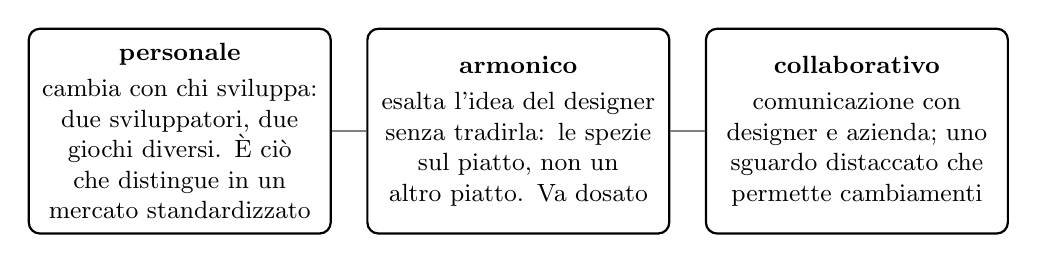
\begin{tikzpicture}[
  font=\small,
  a13pr/.style={draw, thick, rounded corners=4pt, text width=3.6cm, align=center,
                minimum height=2.6cm, fill=white},
]
  \node[a13pr] (p1) at (0,0) {\textbf{personale}\\[2pt]cambia con chi sviluppa: due
    sviluppatori, due giochi diversi. È ciò che distingue in un mercato
    standardizzato};
  \node[a13pr] (p2) at (4.3,0) {\textbf{armonico}\\[2pt]esalta l'idea del designer senza
    tradirla: le spezie sul piatto, non un altro piatto. Va dosato};
  \node[a13pr] (p3) at (8.6,0) {\textbf{collaborativo}\\[2pt]comunicazione con designer
    e azienda; uno sguardo distaccato che permette cambiamenti};
  \draw[thick, gray] (p1) -- (p2) -- (p3);
\end{tikzpicture}
\caption{I tre principi dello sviluppo secondo Marta.}
\label{a13:fig:principi}
\end{figure}

% ---------------------------------------------------------------------
\section{Gli \emph{stakeholder}: chi ha voce sul gioco}
\label{a13:sec:stakeholder}

\slidefig{img/AGD/agd13-stakeholder}{Gli stakeholder.}{slide \emph{Sviluppo di giochi}}{fig:agd13-stakeholder}


Chi sono, più nel dettaglio, gli \emph{stakeholder} tra cui lo sviluppo media? I primi
due sono già emersi: \textbf{il designer} (o la designer) e \textbf{la casa editrice}. Ma
una parte che ``molto spesso viene trascurata e tralasciata'' è \textbf{chi poi gioca il
gioco}: i clienti, le clienti. Quando si fa un gioco è importante ricordarsi \textbf{per
chi lo si sta facendo}, e quella è proprio la voce che non si sente: in una riunione
sul gioco c'è la casa editrice, nella veste del direttore editoriale, c'è l'autore o
l'autrice, ma \textbf{non c'è chi poi lo compra e lo gioca}, ``perché non si può''. Al
massimo si prendono dei \emph{playtester}, ma è una visione parziale; oppure, con un po'
di esperienza del mercato e delle persone a cui il gioco arriva, si può \textbf{fare le
veci di quella parte}. Marta lo fa spesso: ``sì, ma questa modifica va nell'interesse di
chi compra il gioco? Magari è una cosa che piace a noi qua dentro, ma a chi lo compra non
interessa''.

Non è detto che le tre parti ci siano sempre: quando c'è una casa editrice è probabile
che ci sia anche un cliente, ma possono mancare altre parti, o essercene altre ancora.
Se il gioco è \textbf{su licenza}, uno \emph{stakeholder} è \textbf{chi ha fornito la
licenza}, che ha i suoi vincoli e i suoi paletti. Può esserci una persona che ha
\textbf{scritto il \emph{world building}} del gioco e vuole che venga mantenuto in un
certo modo. ``Anche qua potrebbero esserci molte più variabili di quelle che viene da
pensare in prima battuta.''

\begin{figure}[htbp]
\centering
\begin{tikzpicture}[
  font=\small,
  a13st/.style={draw, thick, rounded corners=4pt, text width=2.7cm, align=center,
                minimum height=1.1cm, fill=white},
  a13opt/.style={draw, thick, dashed, rounded corners=4pt, text width=2.7cm, align=center,
                 minimum height=1.1cm, fill=white},
  a13arr/.style={{Stealth[length=2.5mm]}-{Stealth[length=2.5mm]}, thick}
]
  \node[draw, very thick, circle, fill=gray!15, minimum size=2.4cm, align=center] (sv)
    at (0,0) {\textbf{sviluppo}\\(mediazione)};
  \node[a13st] (des) at (-4.2,1.6) {\textbf{designer}\\la visione originale};
  \node[a13st] (pub) at (4.2,1.6) {\textbf{casa editrice}\\catalogo, mercato,
    reparti};
  \node[a13st, fill=gray!8] (cli) at (0,-2.9) {\textbf{chi gioca}\\(la voce che non c'è
    alle riunioni)};
  \node[a13opt] (lic) at (-4.2,-1.6) {chi ha dato la \textbf{licenza}};
  \node[a13opt] (wb) at (4.2,-1.6) {chi ha scritto il \textbf{\emph{world building}}};
  \foreach \n in {des,pub,cli}{\draw[a13arr] (sv) -- (\n);}
  \foreach \n in {lic,wb}{\draw[a13arr, dashed] (sv) -- (\n);}
\end{tikzpicture}
\caption{Gli \emph{stakeholder} di un gioco secondo la lezione. In tratteggio quelli che
ci sono solo in alcuni progetti. La voce di chi gioca arriva solo attraverso i
\emph{playtest} o attraverso chi sviluppa, che con l'esperienza ne fa le veci.}
\label{a13:fig:stakeholder}
\end{figure}

\paragraph{Approfondimento: partecipanti e ``avvocati''.} Bateman e Boon, in \emph{21st
Century Game Design}, aprono il libro con un principio che chiamano \emph{Zen Game
Design}: ``il game design deve essere privo di ego, bilanciando i desideri e i bisogni di
tutti i partecipanti''. I \emph{partecipanti} sono chiunque abbia un interesse nel
progetto (il pubblico, l'editore, lo studio, i programmatori, gli artisti, il marketing,
e, ``sempre più spesso'', il \emph{detentore della licenza}); poiché non tutti possono
partecipare al \emph{design}, alcune figure fanno da \emph{advocate}, da portavoce, per
gli altri. Gli autori notano proprio ciò che nota Marta: per il pubblico, di solito,
\emph{non c'è} un portavoce formale, e il compito ricade su chi progetta; e a proposito
della licenza consigliano di tenere aperto il dialogo durante tutto lo sviluppo, invece di
mostrare il gioco finito al licenziatario ed essere costretti a cambiarlo quando i
cambiamenti costano di più. Il libro parla di videogiochi, e di \emph{designer} più che
di sviluppatori, ma la figura che Marta descrive (chi si fa carico delle voci assenti)
corrisponde quasi esattamente al loro \emph{advocate}.

% ---------------------------------------------------------------------
\section{\emph{Design} contro sviluppo}
\label{a13:sec:designvs}

\slidefig{img/AGD/agd13-design}{Design e sviluppo a confronto.}{slide \emph{Sviluppo di giochi}}{fig:agd13-design}


Qui arriva, dice Marta, ``la differenza più sostanziale'' tra \emph{design} e sviluppo.
Avverte subito che è una visione ``un po' stereotipica'': non è detto che chi fa
\emph{design} abbia tutte queste caratteristiche, né chi fa sviluppo tutte le altre; ma
è ``una buona cartina di tornasole'' per distinguere le due figure. Il confronto è
riassunto nella tabella~\ref{a13:tab:designvs}.

\paragraph{Chi fa \emph{design}.}
\begin{itemize}
  \item \textbf{Non è \emph{time driven}}: normalmente non ha una scadenza vera e propria.
        Può pensare a una scadenza nel senso di ``questo \emph{design} tra cinque anni non
        è più interessante'', ma di base non ha ristrettezze temporali. Diverso è il caso di
        un \emph{design} su commissione.
  \item Ha \textbf{piena libertà creativa}: può muoversi liberamente, presentare qualsiasi
        idea e cercare il canale giusto per pubblicarla, senza vincoli.
  \item Ha di solito un \textbf{attaccamento emotivo}: il gioco l'ha creato, c'è qualcosa
        di suo. È positivo, perché permette di mettere nel gioco caratteristiche che una
        persona senza quell'amore per il progetto non metterebbe; ed è negativo, perché
        rende difficile fare modifiche, e a volte stravolgimenti, ``perché magari ci si è
        affezionati''.
  \item Ha l'\textbf{originalità}: si può prendere qualsiasi cosa e metterla dentro.
        ``Vado a prendere dei cubetti d'oro, di oro vero, e li metto nel gioco'':
        chi fa \emph{design} potrebbe volerlo fare, e il \emph{design} non lo impedisce; il
        problema, semmai, sarà della casa editrice. Ed è proprio lì che vengono fuori le
        cose ``un po' rivoluzionarie'' che a volte servono per smuovere i mercati, per
        alzare l'asticella.
  \item Ha \textbf{un'idea}: l'idea di partenza è ciò che caratterizza il \emph{design}.
        Non deve essere ``fatta e finita'', né completamente bilanciata, né
        completamente finalizzata: deve far capire le intenzioni. Negli anni c'è stata una
        \textbf{professionalizzazione del \emph{design}}, e oggi i designer portano in
        genere il progetto molto più avanti che in passato; ma resta la possibilità di
        dichiarare chiusa un'idea in qualsiasi momento (``questo è sufficiente per far
        capire che cosa dovrebbe essere sviluppato'') e consegnarla a una casa editrice.
\end{itemize}

\paragraph{Chi fa sviluppo.}
\begin{itemize}
  \item Ha \textbf{scadenze}: il \textbf{\emph{time to market}}, cioè quando il gioco deve
        uscire per prendere la spinta giusta del mercato, e il \textbf{vincolo del
        contratto} firmato tra casa editrice (o chi sviluppa) e designer. A un certo punto
        il gioco deve uscire, essere finalizzato, completato.
  \item Ha \textbf{restrizioni produttive}: tornando ai cubetti d'oro, ``io poi devo fare i
        conti con la realtà di mettere dei cubetti d'oro su mille scatole''. Come si fa?
        Sono veramente necessari? Sono veramente la cosa che serve?
  \item Esercita il \textbf{distacco}: non avendo un legame emotivo con il progetto,
        soprattutto all'inizio, può analizzarlo in modo più freddo e riconoscere quali
        caratteristiche servono all'idea per funzionare sul mercato, per certi clienti.
  \item Porta la \textbf{standardizzazione}, che ha due facce. È positiva perché un'idea
        troppo originale può spaventare alcune fette di mercato: un gioco molto originale
        viene recepito ``in modo misto, se va bene'', spesso male, perché il mercato ``non
        è pronto'', non aveva in mente quel gioco. La standardizzazione \textbf{smussa gli
        angoli}, rende il gioco più digeribile, più simile ad altre cose. Ma smussare gli
        angoli rischia anche di \textbf{portare via le caratteristiche importanti} del
        gioco.
  \item Ha l'\textbf{esperienza}\footnote{In questo punto la trascrizione è coperta da
        alcune righe di frasi ripetute senza senso (``è falsata da un pubblico''); la
        quinta voce della slide si ricostruisce dal discorso che segue e dalla sezione
        successiva, dedicata proprio all'esperienza.}: un designer che ha fatto un solo
        gioco ha ``pochissima'' esperienza, mentre chi fa sviluppo ha in genere lavorato a
        più titoli, perché si muove più rapidamente tra più progetti. Sa già dire ``questa
        cosa su itch.io non funziona, perché se lo pubblichi così le persone non capiscono
        neanche che tipo di gioco è: perché non evidenziamo questi aspetti?''. Un prodotto
        sullo scaffale, o caricato su itch.io, funziona?
\end{itemize}

\begin{table}[htbp]
\centering
\small
\begin{tabular}{@{}p{3.0cm}p{5.0cm}p{5.4cm}@{}}
\toprule
 & \textbf{Chi fa \emph{design}} & \textbf{Chi fa sviluppo} \\
\midrule
Tempo & non \emph{time driven} (salvo commissione) & scadenze: \emph{time to market},
  contratto \\
Libertà & piena libertà creativa & restrizioni produttive (i ``cubetti d'oro'' su mille
  scatole) \\
Rapporto col gioco & attaccamento emotivo (pro e contro) & distacco, analisi ``fredda'' \\
Direzione & originalità, anche rivoluzionaria & standardizzazione: smussa gli angoli
  (pro e contro) \\
Che cosa porta & un'idea, anche non finita & esperienza su molti titoli e generi \\
\bottomrule
\end{tabular}
\caption{\emph{Design} contro sviluppo secondo la slide di Marta: una visione volutamente
``stereotipica'', utile come cartina di tornasole. Nella realtà i confini sono sfumati.}
\label{a13:tab:designvs}
\end{table}

\paragraph{Confini sfumati.} Che cosa succede se un'idea è \textbf{troppo embrionale}? O se
un'implementazione che si va a fare \textbf{cambia l'esperienza di gioco}? ``Queste sono
domande importantissime, dove le cose si sfumano.'' A volte si ricevono idee così
embrionali che quasi non converrebbe prenderle, perché c'è così tanto sviluppo da fare
che non si sa più quanto è sviluppo e quanto è \emph{design}. Dall'altra parte c'è il
rischio che fare sviluppo \textbf{comprometta l'esperienza originale}. Questi ruoli vanno
immaginati come ``qualcosa di molto permeabile'', e non è mai facile mettere l'asticella
nel punto giusto: ``io molto spesso me lo chiedo: ma per questo gioco ho fatto
effettivamente sviluppo? Sono arrivata addirittura a fare \emph{design}?''. Con
l'esperienza diventa più facile tracciare la linea: capire se l'idea è davvero troppo
embrionale, e quindi non conviene svilupparla, o se c'è stato un eccesso (``ho fatto
troppo sviluppo, ho cambiato l'idea di partenza'') e bisogna tornare sui propri passi e
far emergere di più l'idea originale del designer.

% ---------------------------------------------------------------------
\section{Lo sviluppo è esperienziale}
\label{a13:sec:esperienza}

Marta lo ha detto più volte: lo sviluppo \textbf{si fonda sull'esperienza}. Da qualche
parte si parte, ``ci si improvvisa un po', come in tutte le cose'', ma poi l'esperienza si
accumula e fa la differenza. Non c'è un modo esatto di accumularla, ma c'è una differenza
di fondo tra le due figure.

\paragraph{Il designer focalizzato.} Chi fa \emph{design} può fare continuamente lo stesso
\emph{design}, senza esplorare tanti giochi e tante idee diverse. L'esempio è \textbf{Uwe
Rosenberg}\footnote{Nella trascrizione solo ``Rosenberg''; dal contesto (piazzamento
lavoratori, piazzamento tessere) è quasi certamente Uwe Rosenberg, l'autore di
\emph{Agricola}, citato più avanti nella lezione.}, che ha ``tre o quattro temi'' e tende
a fare giochi su quelli: il piazzamento lavoratori, il piazzamento tessere, e poi qualche
esperimento su altri generi. Una visione non ristretta in senso negativo, precisa Marta:
``\textbf{focalizzata} è il termine giusto''. Una visione che, nella sua iteratività, lo ha
portato a raggiungere \textbf{l'apice dei generi} in cui ha lavorato, perché li ha
``talmente tanto sviscerati'' da conoscerne forze e debolezze.

\paragraph{Lo sviluppatore che tocca tutto.} Chi sviluppa, al contrario, entra in contatto
con \textbf{tantissimi generi diversi}, perché le idee non vengono sempre dalla stessa
persona. Marta ha sviluppato giochi che durano più di due ore, giochi leggeri,
\emph{party game}, giochi di destrezza astratti: ``si tocca un po' tutto quello che
esiste''. Vale anche per il gioco di ruolo, dove chi sviluppa può muoversi più facilmente
tra sistemi diversi, dal gioco di una pagina (\emph{one page}) al manuale di 50 pagine con
campagna.

% ---------------------------------------------------------------------
\section{Il rapporto tra chi progetta e chi sviluppa}
\label{a13:sec:rapporto}

\slidefig{img/AGD/agd13-rapporto}{Il rapporto tra designer e developer.}{slide \emph{Sviluppo di giochi}}{fig:agd13-rapporto}


L'esperienza passa anche attraverso il \textbf{rapporto tra designer e \emph{developer}},
che ``deve essere saputo gestire'': per le differenze appena viste, per i livelli diversi
di esperienza, per i ruoli diversi, che a volte sembrano perfino contrapposti. Ma è, come
detto all'inizio, un rapporto di mediazione, e la cosa importante è \textbf{trovare i
compromessi}. Ogni rapporto è diverso: non si lavora con tutti i designer nello stesso
modo.

\paragraph{Collaborazione attiva e passiva.} A Marta sono capitate entrambe.
\begin{itemize}
  \item Una \textbf{collaborazione attiva} è uno \textbf{scambio ricorrente} tra le due
        parti: ci si aggiorna a vicenda, si fanno cambiamenti, ``ci si rimbalzano molto le
        idee e il progetto''.
  \item Una \textbf{collaborazione passiva} è quando una delle due parti prende in carico
        la maggior parte del lavoro e \textbf{riceve dei \emph{feedback}} dall'altra, e il
        rapporto si limita a questo. Può capitare, per esempio, che un gioco venga
        valutato, firmato con la casa editrice, e che poi chi l'ha progettato
        ``praticamente sparisca''. \textbf{È legittimo}: l'idea è stata fornita, i dubbi, se
        c'erano, si spera siano stati risolti, e magari il designer non ha interesse a
        vedere come si sviluppa il gioco da lì in poi, e vuole vederlo solo a cose fatte.
\end{itemize}

\paragraph{Le aspettative.} È importante anche \textbf{gestire le aspettative}: ricordarsi
che quando un gioco passa per altre persone \textbf{viene inevitabilmente modificato}.
``Un gioco è un processo di collaborazione'': non c'è una sola persona che lo fa. La
figura del designer è stata più volte messa in primo piano, ma il processo è
\textbf{collettivo}: il gioco non arriverebbe sullo scaffale senza chi lo produce, chi fa
la grafica e le illustrazioni, e chi lo sviluppa. Affidando un gioco a una casa editrice
o a chi sviluppa, il gioco \textbf{cambierà}, anche in modi che non sempre troveranno
d'accordo. L'importante è trovare i compromessi giusti.

\paragraph{La fiducia.} E qui viene l'ultimo punto: la \textbf{fiducia}. ``Come se si
vogliono avere delle relazioni nella vita'', bisogna avere una fiducia reciproca. Il
consiglio di Marta, anche ai designer: \textbf{cercatevi case editrici, sviluppatori o
sviluppatrici con cui pensate che possa esserci un buon rapporto di fiducia}, perché i
rapporti vanno male soprattutto quando questa fiducia viene a mancare, quando una delle
due parti pensa che l'altra ``non stia facendo gli interessi del gioco''.

% ---------------------------------------------------------------------
\section{Da dove viene il ruolo: \emph{developer} ed \emph{editor}}
\label{a13:sec:storia}

\slidefig{img/AGD/agd13-storia}{Brevi cenni storici sullo sviluppo.}{slide \emph{Sviluppo di giochi}}{fig:agd13-storia}


``Vi siete chiesti chi è l'\emph{editor}, in questo calderone?'' Per rispondere Marta
racconta da dove nasce la figura dello sviluppo.

\paragraph{Gli anni Settanta e i \emph{wargame}.} Siamo negli anni '70, e la
\textbf{SPI}, \emph{Simulations Publications, Inc.}\footnote{Marta dice ``Simulation
Publishing Inc., credo''; il nome corretto della casa editrice americana di
\emph{wargame} è \emph{Simulations Publications, Inc.}}, una casa editrice americana di
\emph{wargame}, ha bisogno di pubblicare \textbf{più \emph{wargame}}: chi fa \emph{design}
``non ce la fa a fare tutti questi''. A questo punto la trascrizione si interrompe per
alcune frasi ripetute senza senso, e una parte del racconto va perduta\footnote{Coprono
la spiegazione di come la SPI risolse il problema. Il capitolo non la ricostruisce; si
sa, in generale, che nella SPI il \emph{developer} era la figura che riceveva il
\emph{design} e lo portava a un gioco pubblicabile, ma la trascrizione non permette di
dire che cosa abbia detto Marta.}. Quando il discorso riprende, Marta sta elencando le
case editrici che, dopo, hanno deciso di \textbf{inserire degli sviluppatori}:
\textbf{Fantasy Flight}, la linea \textbf{\emph{alea}} di Ravensburger e \textbf{Hans im
Glück}\footnote{Nella trascrizione ``la linea Alia di Ravensburger'' e ``Huntington
Gluck'', poi ``Hansingluck''.}. Gli sviluppatori sono ``fondamentalmente delle figure che
fanno le veci dei designer all'interno delle aziende'', ma \textbf{non sono designer in
senso stretto}: avranno idee e visioni diverse, ed è qui che nasce il rapporto
collaborativo come lo conosciamo oggi.

\paragraph{L'\emph{editor} tedesco.} Contemporaneamente c'era un'altra figura,
l'\textbf{\emph{editor}}, molto diffusa in \textbf{Germania}: era la persona che si
occupava di \textbf{portare il gioco a compimento}. Le altre case editrici tedesche avevano
un \emph{editor}, e lo avevano anche \emph{alea} e Hans im Glück; ma l'\emph{editor}
\textbf{non si occupava del gioco nell'aspetto meccanico e regolistico}: si occupava di
tutti gli altri aspetti.

\paragraph{L'inversione.} Andando avanti le due figure \textbf{si sono ibridate}, e oggi si
sono ``un po' invertite'': lo \textbf{sviluppo}, che prima si occupava solo della parte
meccanica, oggi prende in carico \textbf{tutti gli aspetti}, compresa la parte meccanica;
l'\textbf{\emph{editor}} ha un ruolo più piccolo, legato soprattutto \textbf{alle parole}:
rivede i testi, controlla che siano in italiano corretto, si accerta che tutto sia
presentato al meglio. Questa è, oggi, la figura che di solito si chiama \emph{editor} nel
gioco da tavolo. Ma non è definito in modo assoluto: ci sono case editrici che chiamano
``sviluppatore'' chi fa \emph{editing}, e case che fanno \emph{editing} e non hanno
sviluppatori. È una figura nata negli ultimi anni e \textbf{non c'è ancora una
standardizzazione}; questa, confrontandosi con colleghi e colleghe di altre aziende, è la
tendenza che Marta vede.

\begin{figure}[htbp]
\centering
\begin{tikzpicture}[
  font=\small,
  a13ev/.style={draw, thick, rounded corners=3pt, text width=3.5cm, align=center,
                minimum height=1.4cm, fill=white},
  a13arr/.style={-{Stealth[length=3mm]}, thick}
]
  \draw[a13arr] (0,0) -- (13.4,0);
  \foreach \x/\lab in {1.6/anni '70, 6.4/poi, 11.4/oggi}{
    \fill (\x,0) circle (2.5pt);
    \node[below=4pt, font=\footnotesize] at (\x,0) {\lab};
  }
  % sopra: developer
  \node[a13ev, above=0.5cm] at (1.6,0) {SPI (\emph{wargame}): servono più giochi di quanti
    i designer riescano a farne};
  \node[a13ev, above=0.5cm] at (6.4,0) {Fantasy Flight, \emph{alea} (Ravensburger), Hans
    im Glück inseriscono gli \textbf{sviluppatori}: parte meccanica};
  \node[a13ev, above=0.5cm, fill=gray!12] at (11.4,0) {\textbf{sviluppo}: tutti gli
    aspetti, meccanica compresa};
  % sotto: editor
  \node[a13ev, below=0.7cm] at (6.4,0) {l'\textbf{\emph{editor}} (soprattutto in Germania)
    porta il gioco a compimento, \emph{tranne} meccanica e regole};
  \node[a13ev, below=0.7cm, fill=gray!12] at (11.4,0) {\textbf{\emph{editor}}: le parole,
    i testi, la presentazione};
  \node[font=\footnotesize\itshape, rotate=90] at (-0.4,1.4) {\emph{developer}};
  \node[font=\footnotesize\itshape, rotate=90] at (-0.4,-1.5) {\emph{editor}};
\end{tikzpicture}
\caption{Come Marta racconta la nascita delle due figure e la loro ``inversione''. Le
date intermedie non sono dette, e una parte del racconto è persa nella trascrizione. Oggi
le definizioni non sono ancora standardizzate.}
\label{a13:fig:storia}
\end{figure}

\paragraph{Prima pausa.} ``Siamo alla seconda parte'': Marta propone una pausa di una
decina di minuti e invita a portare domande al ritorno. Durante la pausa la trascrizione
registra il commento su un videogioco di cui si è detto nelle avvertenze, e poi diversi
minuti di frasi ripetute in ciclo. Quando si riprende, uno studente avverte che sta
ancora mangiando, ``ma ci sono, nessun problema''. Marta chiede se ci sono domande o
curiosità (``non so se vi posso rispondere in pieno, perché c'è una parte di segreto
professionale, ma possiamo ingegnarci'').

% ---------------------------------------------------------------------
\section{Il conflitto di interessi}
\label{a13:sec:conflitto}

La prima domanda è di \textbf{Gianmarco}\footnote{Più avanti Marta si riferisce a questa
domanda come ``quella domanda che ha fatto Gianmarco''.}, ``fra la curiosità e la
provocazione'': lo sviluppatore, di solito, è \textbf{assunto dalla casa editrice}, mentre
il designer non lo è necessariamente. \textbf{Non c'è un conflitto di interessi} nel fare
da mediatore tra due parti, quando si è assunti da una delle due? ``È un'ottima domanda,
onestamente'', risponde Marta, ``non so neanche se riuscirò a soddisfarti''.

\paragraph{Com'era prima.} All'inizio la figura non c'era, e il rapporto era diverso: i
designer avevano un gioco e la casa editrice si limitava a \textbf{metterlo sul mercato
così com'era stato pensato}; rivedeva i testi, curava la produzione fisica. ``Addirittura
i designer brevettavano i tabelloni'': erano tempi diversi. Funzionava quando \textbf{il
mercato era piccolo}, le idee erano poche e c'era tantissimo spazio per presentarle.

\paragraph{Com'è oggi.} Oggi a \textbf{Essen}, la più grande fiera al mondo di giochi da
tavolo, secondo le ultime stime che Marta ricorda si parla di qualcosa come \textbf{2500
nuovi giochi presentati in un solo anno}, e solo tra quelli pubblicati in qualche forma,
senza contare tutta la realtà indipendente che pubblica su itch.io e simili. ``Il volume
di giochi presentati ogni anno è spaventoso.'' Le case editrici, molto spesso,
\textbf{non possono permettersi di sbagliare un titolo} (``cannare'', dice Marta): dipende
dalle dimensioni, ma una piccola casa editrice che sbaglia anche solo un paio di titoli
può chiudere, perché \textbf{l'investimento nel gioco analogico è importante}. Per questo la
cosa fondamentale è che il gioco \textbf{rispetti le aspettative di mercato}. E chi fa
\emph{design} non è tenuto a conoscerle, e probabilmente non ha i mezzi per farlo: Marta
non conosce ``tantissime designer'' che abbiano la possibilità di andare a Essen e
interfacciarsi con più editori, anche internazionali. È un limite, e oggi \textbf{avere
dentro l'azienda una figura che fa le tue veci} per tutte queste questioni è generalmente
visto come positivo, anche se non vale per tutte le persone.

\paragraph{Che cosa fa Marta.} Marta sconsiglia spesso di fare giochi \textbf{solo con
l'obiettivo di pubblicare con una casa editrice}: capisce che i soldi facciano gola, ma
bisogna saper riconoscere \textbf{quali giochi sono adatti al mercato}, trovare la casa
editrice che fa per noi e vedere se con le persone con cui si collabora ci si trova bene.
Lei, da parte sua, cerca di \textbf{rispettare le volontà del designer}, proprio perché sa
di essere assunta dalla casa editrice, ma anche di essere, in quel momento,
\textbf{l'unica persona che sta parlando per il designer}, che magari non c'è a tutte le
riunioni: diventa importante difendere le sue idee. Si rende conto che non è sempre
facile, e che non è facile nemmeno accettare la dinamica. ``In un mondo ideale'' chi fa
\emph{design} potrebbe partecipare attivamente alle quaranta ore lavorative in azienda in
cui si fanno le cose; nella realtà le dinamiche sono complesse. Gianmarco si dice
soddisfatto: ``mi è abbastanza chiara la risposta''.

\paragraph{Approfondimento: il portavoce assunto.} La domanda di Gianmarco è la stessa che
Bateman e Boon si pongono a proposito del produttore esterno, il portavoce dell'editore
nei progetti di videogiochi: secondo loro molti sviluppatori ne risentono
l'``interferenza'', ma il problema nasce di solito quando il portavoce cerca di
\emph{prendersi il controllo} del \emph{design}, invece di rappresentare i bisogni di chi
rappresenta. La risposta di Marta sposta il problema nello stesso punto: il ruolo regge
finché chi sviluppa si comporta da mediatore, e dà voce anche a chi, in quella stanza, non
c'è.

% ---------------------------------------------------------------------
\section{Le otto fasi dello sviluppo}
\label{a13:sec:fasi}

\slidefig{img/AGD/agd13-fasi}{Le otto fasi dello sviluppo.}{slide \emph{Sviluppo di giochi}}{fig:agd13-fasi}


Oggi, ripete Marta, si fa un'infarinatura generale; la prossima volta qualche esempio più
pratico e qualche tecnica. ``La realtà della faccenda è che \textbf{non c'è un modo esatto
di procedere}'': ogni gioco fa storia a sé, e non si sviluppa un gioco totalmente
narrativo come si sviluppa un gioco di destrezza. Raccomanda di \textbf{pensare in modo
elastico}, perché è facile farsi ingannare e pensare che le cose siano lineari: ``non è mai
così''. Ed è anche l'aspetto bello del lavoro: c'è sempre una sfida nuova. ``Io mi sono
improvvisamente scoperta appassionata di bonsai soltanto perché ho lavorato a un gioco che
parlava di bonsai'': se si è persone curiose, ``è un bel lavoro''.

Marta ha riassunto il lavoro in \textbf{otto fasi} (figura~\ref{a13:fig:fasi}):
\textbf{selezione}, \textbf{ricerca}, \textbf{concettualizzazione},
\textbf{presentazione}, \textbf{\emph{testing}}, \textbf{implementazione},
\textbf{preparazione degli \emph{asset}}, \textbf{revisioni}. È, grosso modo, la
\emph{pipeline} di un gioco dal primo momento in cui viene accettato nel ramo di sviluppo
di un'azienda a quando lascia l'azienda per essere stampato e finire sullo scaffale. Le
fasi \textbf{non si svolgono necessariamente in quest'ordine}: a volte si torna indietro, a
volte mancano dei pezzi; c'è tanto scambio e tanto dialogo con tutti i reparti per
arrivare alla fine ``nel modo più celere possibile'', ma ``molto spesso arrivano i
disastri e bisogna tornare indietro''. In questa lezione Marta arriva fino alla
preparazione degli \emph{asset}; le \textbf{revisioni} e il \textbf{come scrivere un
regolamento} restano per venerdì (sezione~\ref{a13:sec:chiusura}).

\begin{figure}[htbp]
\centering
\begin{tikzpicture}[
  font=\small,
  a13ph/.style={draw, thick, rounded corners=3pt, text width=2.3cm, align=center,
                minimum height=1.0cm, fill=white},
  a13arr/.style={-{Stealth[length=2.5mm]}, thick}
]
  \node[a13ph] (f1) at (0,1.6) {1.\ selezione};
  \node[a13ph] (f2) at (3.1,1.6) {2.\ ricerca};
  \node[a13ph] (f3) at (6.2,1.6) {3.\ concettua-\\lizzazione};
  \node[a13ph] (f4) at (9.3,1.6) {4.\ presentazione};
  \node[a13ph] (f5) at (9.3,-0.6) {5.\ \emph{testing}};
  \node[a13ph] (f6) at (6.2,-0.6) {6.\ implementa-\\zione};
  \node[a13ph] (f7) at (3.1,-0.6) {7.\ preparazione\\degli \emph{asset}};
  \node[a13ph, fill=gray!12] (f8) at (0,-0.6) {8.\ revisioni\\(venerdì)};
  \draw[a13arr] (f1) -- (f2);
  \draw[a13arr] (f2) -- (f3);
  \draw[a13arr] (f3) -- (f4);
  \draw[a13arr] (f4) -- (f5);
  \draw[a13arr] (f5) -- (f6);
  \draw[a13arr] (f6) -- (f7);
  \draw[a13arr] (f7) -- (f8);
  \draw[a13arr, dashed] (f2.north) to[bend right=35] node[above, font=\footnotesize]
    {si torna indietro} (f1.north);
  \draw[a13arr, dashed] (f6.south) to[bend right=40] node[below, font=\footnotesize]
    {ogni ciclo di \emph{test}} (f5.south);
  \draw[a13arr, dashed] (f5.south west) to[bend left=25] (f6.south east);
  \node[font=\footnotesize, text width=4.2cm, align=left, anchor=west] at (-1.2,-2.9)
    {\emph{ingresso}: un prototipo accettato};
  \node[font=\footnotesize, text width=4.2cm, align=right, anchor=east] at (10.5,-2.9)
    {\emph{uscita}: il gioco va in stampa};
\end{tikzpicture}
\caption{Le otto fasi dello sviluppo secondo Marta. L'ordine è indicativo: le frecce
tratteggiate ricordano che si torna spesso indietro (per esempio la ricerca informa la
selezione, e implementazione e \emph{testing} si alternano in ciclo).}
\label{a13:fig:fasi}
\end{figure}

% ---------------------------------------------------------------------
\section{La selezione}
\label{a13:sec:selezione}

\slidefig{img/AGD/agd13-selezione}{La selezione.}{slide \emph{Sviluppo di giochi}}{fig:agd13-selezione}


La selezione comincia quando si riceve un \textbf{prototipo}, e se ne ricevono
\textbf{tantissimi}. Marta non sa fare una stima precisa, perché cambia molto da periodo a
periodo e da casa editrice a casa editrice; ma nell'ultimo mese, se non sbaglia, a dV
Giochi ne sono arrivati \textbf{una sessantina}. dV è una casa editrice grande, e altre ne
ricevono meno; ma si immagini di dover valutare 60 prototipi al mese: ci deve essere
\textbf{una cernita}, e avviene in vari modi.

\begin{itemize}
  \item \textbf{Catalogo e mercato di riferimento.} C'è una scrematura iniziale legata al
        catalogo. dV Giochi non pubblica giochi che superano i \textbf{45 minuti, un'ora}:
        se arriva un gioco che dura due ore e mezza, probabilmente viene scartato a
        priori, perché è molto improbabile che faccia al caso loro. Un'occhiata si dà
        sempre, però: magari c'è un'idea buona, magari le due ore e mezza sono una stima
        sbagliata dell'autore.
  \item \textbf{La complessità.} Un buon gioco può risultare \textbf{eccessivamente
        complesso}, nel senso che è difficile da spiegare e da far capire, e allora non ci
        sono i margini per provarlo e testarlo adeguatamente: ``magari devo studiarmi un
        regolamento per quattro giorni, e io quattro giorni da passare a provare un gioco
        non ce li ho''. Va valutato: è un gioco che si può testare con il designer? Fa
        davvero al caso nostro?
  \item \textbf{La sensibilità del \emph{team} editoriale.} Lo sviluppo è personale, e
        questo si riflette in tutto: ``se non ci piacciono i giochi in tempo reale, è
        inutile che pensiamo che quel gioco in tempo reale funzioni benissimo'', perché se
        poi non riusciamo a metterci a svilupparlo stiamo solo perdendo tempo. In ambito
        professionale non contano solo le preferenze (``altrimenti io svilupperei solamente
        due tipi di giochi''), ma ci sono giochi che si sa che non funzioneranno con quel
        \emph{team}. Marta, per esempio, ``non è ferratissima'' sui \textbf{giochi di
        destrezza}: tende a evitarli o a passarli a un collega (``tu che hai più la
        sensibilità per questa cosa, ci vedi qualcosa in questo gioco?''), perché anche
        fisicamente fa fatica a valutarli. Una casa editrice brava riesce a riflettere
        queste sensibilità nel suo catalogo. E bisogna tenerle a mente perché i giochi
        selezionati vanno poi testati, provati, discussi con i designer: ``quello che inizia
        come un processo di un'ora, un'ora e mezzo potrebbe diventare tranquillamente di
        giorni''.
  \item \textbf{La coerenza sull'asse tema--meccaniche.} Negli ultimi anni ci sono
        tantissimi giochi che si assomigliano. Una volta si tendeva a privilegiare uno dei
        due aspetti, di solito le meccaniche, e poi c'era il cosiddetto \textbf{\emph{window
        dressing}}: si ``appiccicava'' sopra un tema che giustificasse un po' le
        meccaniche. Negli anni questo ha portato a una \textbf{stagnazione}, e oggi c'è
        anche ``un po' di pesantezza'' da questo punto di vista. Oggi è molto importante che
        \textbf{meccaniche e tema si parlino in modo molto stretto}. Questo significa che il
        gioco si può modificare di meno, e che c'è più rischio che non venga accettato:
        ``lato designer è un incubo'', perché si lavora a un gioco per tantissimo tempo e
        poi non viene accettato perché non piace il tema, e se il legame è forte non si
        può più dire ``cambia il tema, qual è il problema?''. Ma è anche ciò che oggi fa
        scegliere un gioco sopra gli altri. L'esempio è \textbf{\emph{Hegemony}}\footnote{Nella
        trascrizione ``Egemoni''; si tratta con ogni probabilità di \emph{Hegemony: Lead
        Your Class to Victory}, un gioco gestionale sulle classi sociali e sulla politica
        economica di uno Stato.}, un gioco gestionale (``vedo un sì'', dice Marta quando
        chiede se la classe lo conosce) che ricrea le dinamiche della politica di uno Stato
        ``in modo molto viscerale'': è una simulazione astratta, ma i designer hanno legato
        le meccaniche al tema ``in modo indissolubile''. Non si può prendere \emph{Hegemony}
        e farne un gioco sugli esploratori di \emph{dungeon}, ``perché non regge''; mentre su
        un gioco di carte con solo numeri si può mettere il \emph{dungeon}, o un tema
        diverso, perfino politico.
\end{itemize}
Sono criteri generici, ``che ci aiutano a selezionare i giochi più promettenti'', a capire
quali meritano una possibilità di sviluppo.

% ---------------------------------------------------------------------
\section{La ricerca}
\label{a13:sec:ricerca}

\slidefig{img/AGD/agd13-ricerca}{La ricerca.}{slide \emph{Sviluppo di giochi}}{fig:agd13-ricerca}


Dopo la selezione c'è la \textbf{ricerca}. Lo strumento principale, nel mondo del gioco da
tavolo, è \textbf{BoardGameGeek} (BGG): è ``il sito di riferimento'' perché è un
\textbf{\emph{database}}, ed è lo strumento più usato nell'industria, ``con tutti i limiti
che ha'': è una visione \textbf{americano-centrica}, perché la sua utenza è prevalentemente
quella. Ma resta indispensabile, perché vi si trovano tantissime informazioni.

\paragraph{Le domande della ricerca.} Si immagini di aver appena visto, e accettato, il
prototipo di \emph{Hegemony}: un gioco sulla politica e sugli Stati. Prima di tutto
bisogna capire:
\begin{itemize}
  \item ce ne sono altri sul mercato che fanno già la stessa cosa?
  \item se sì, che cosa fanno di diverso?
  \item quali caratteristiche li esaltano, o li affossano?
  \item come sono percepiti dalle persone?
  \item che cosa si può fare di diverso? Magari l'idea è valida, ma approfondendo si scopre
        che ci sono tanti giochi sulla politica di uno Stato: che cosa fa di diverso
        questo?
\end{itemize}
Si conoscono così i temi comuni: andando su BGG e guardando la classifica
\textbf{\emph{hotness}} del periodo, o leggendo le recensioni, emerge per esempio come
negli ultimi anni l'\textbf{asimmetria}\footnote{Nella trascrizione ``la simmetria'', qui e
più avanti (``\emph{Root} con la simmetria''); dal contesto, e dall'esempio di
\emph{Root}, che è il gioco asimmetrico per eccellenza, si tratta quasi certamente di un
errore di trascrizione per ``asimmetria''.} sia diventata una caratteristica molto
importante dei giochi di una certa complessità. Ci si crea anche delle
\textbf{metriche}: ``oggi vanno di più i giochi di dadi''. E qui si torna alla selezione:
``se abbiamo un gioco di dadi, magari è il momento di valutarlo''. È un processo ``che si
informa a sua volta''.

\subsection{Si può prevedere il mercato?}
\label{a13:sec:prevedere}

Uno studente alza la mano con una domanda ``molto complicata'', nata dalla sua esperienza:
ha lavorato molti anni nell'\textbf{\emph{automotive}}. Quando si progetta un'automobile si
prende a riferimento l'esistente: devo fare un nuovo SUV, identifico il cliente, faccio il
posizionamento di prodotto, studio chi c'è in quello spazio e rispetto a quello definisco
le caratteristiche. Ma per fare un'automobile, da foglio bianco, ci vogliono \textbf{dai
quattro ai sei anni}: quattro anni prima dell'uscita si studiano dei concorrenti pensati
sei anni prima. Come si fa, nel gioco, a capire che cosa sarà di tendenza quando il gioco
uscirà, probabilmente due o tre anni dopo la selezione?

\paragraph{``La risposta non piacerà mai a nessuno''.} \textbf{Non c'è un modo di prevedere
il mercato}, ma si può \textbf{affinare la sensibilità}. Su cicli di quattro--sei anni c'è
poco da fare: in sei anni il gioco da tavolo ``subirà degli scossoni importanti''. Prendendo
il 2026 come riferimento: sei anni fa, nel 2020, c'erano giochi che avevano iniziato a
stabilire la propria dimensione, come \textbf{\emph{Root}}, \textbf{\emph{Wingspan}},
\textbf{\emph{Terraforming Mars}}\footnote{Nella trascrizione ``Terraform in Mars''.}; e
questi giochi hanno fatto leva moltissimo su un \textbf{mazzo formato da tutte carte
diverse}, che fa cambiare l'esperienza da una partita all'altra per l'alta variabilità, o,
nel caso di \emph{Root}, sull'asimmetria. Ma sei anni prima ancora ``non c'era neanche
l'antipasto di queste cose'': con il senno di poi si riconosce qualche lieve segno dell'onda
che stava emergendo, ma era ``davvero troppo tempo''. Per questo i \textbf{cicli di
sviluppo} cercano di essere \textbf{il più brevi possibile}, anche se realisticamente è
difficile stare sotto i \textbf{due anni}: Marta ha fatto un conto, e per sviluppare un
gioco servono in media \textbf{nove mesi}; tra produzione e tutto il resto, quando il
gioco finisce sul mercato sono passati due anni.

\paragraph{Curiosità, sempre.} Quello che si può fare è \textbf{curare molto la propria
ricerca}: informarsi, avere curiosità, cercare di capire i giochi quando escono e le loro
peculiarità. Per esempio: \textbf{perché \emph{Magical Athlete} è diventato
improvvisamente così forte}, così centrale nella comunicazione? Che cosa ha fatto bene?
Si possono dare centinaia di risposte diverse; ma facendo questo lavoro la sensibilità si
affina e si riesce a ``vedere un po' in avanti''. È in parte una visione personale, che
viene dalle proprie esperienze, e in parte emerge dal conoscere il settore. Per fare
sviluppo, ``ma a me viene da dire anche per fare \emph{design}'', bisogna avere questa
tendenza a immaginare come sarà il mercato, ``che non significa prenderci in pieno'', ma
avere la sensibilità per capire dove si sta andando.

\paragraph{Il caso \emph{Magical Athlete}.} Quest'anno Marta non è andata a Essen con i
colleghi; al loro ritorno le hanno detto: ``Marta, non ci crederai mai, ma a Essen abbiamo
visto un sacco di prototipi con i dadi''. ``E certo'', ha risposto lei: \emph{Magical
Athlete} ``è uscito l'altro ieri''. Tra i designer è diventato ``una bomba''. Perché? Marta
lo paragona, ``parafrasando'', alla \emph{Fontana} di \textbf{Duchamp}, l'orinatoio esposto
come opera d'arte: un gesto rivoluzionario. \emph{Magical Athlete} è stato un po' quella
cosa lì: ha detto ``e se facessimo il gioco dell'oca, ma ancora più folle?'', e ha
centrato l'obiettivo. La nuova edizione è curata da \textbf{Richard Garfield}, ``che non è
l'ultimo degli arrivati'': è il creatore di \emph{Magic: The Gathering}, e ha fatto molti
altri \emph{design} di spessore. Il gioco, nei circoli di appassionati, era già conosciuto;
ma ha avuto questo ``volano incredibile'' per una ragione precisa.
\begin{itemize}
  \item Analizzando il percorso dei giochi da tavolo, negli ultimi anni la maggior parte
        dei giochi \textbf{davano tantissimo controllo}. Da \textbf{\emph{Agricola}}, uscito
        nel \textbf{2007}, fino al 2026, i giochi hanno esplorato a fondo la meccanica
        dell'avere tutto sotto il proprio controllo, tanto che \emph{Agricola} ha in un
        certo senso inaugurato i giochi \textbf{``multi-solitari''}, come li chiamiamo oggi:
        giochi in cui l'interazione è per lo più passiva, indiretta, in cui ognuno ``si fa
        le sue cose'' e poi si vede chi ha fatto più punti.
  \item La tendenza si è esasperata al punto che serviva una \textbf{risposta forte nella
        direzione opposta}: \emph{Magical Athlete} mette \textbf{tutto il caos possibile},
        fa emergere tutto da una grande interazione tra le persone, ed è un gioco
        \textbf{fortemente esperienziale ed emozionale}. Dice: ``alla fine non ti serve
        davvero tutto questo controllo per stare al tavolo e avere una serata piacevole
        con le persone con cui ti trovi bene''. ``È stato fondamentalmente un messaggio.''
  \item Garfield non ha ``la visione del futuro'', ma ha l'esperienza: ci ha cominciato a
        lavorare, se Marta ricorda bene, nel \textbf{2022}; ha capito che quello era il
        \emph{trend} e che poteva intercettarlo, e ha avuto anche fortuna, perché l'ha
        intercettato probabilmente nel momento di massimo picco, quando le persone
        volevano davvero qualcosa di diverso.
\end{itemize}
Una visione del futuro, quindi, ``un po' ce la si può creare'': si arriva a intravedere le
tendenze, a capire su che cosa si spinge di più. E stare dentro una casa editrice è un
\textbf{punto di vista privilegiato}: Marta conosce ``un sacco di giochi'' che usciranno
prossimamente ma non sono ancora stati annunciati, un po' per i \emph{partner}, un po'
perché nel settore ci si parla.

\paragraph{``Vedi già il prossimo \emph{trend}?''} Lo stesso studente (``non voglio
monopolizzare il discorso, ma ne avrei mille'') chiede ancora: provando i prototipi di
oggi, Marta riesce a intravedere un \emph{trend} che, fra due anni, sarà la reazione a
quello attuale, per esempio a tutti questi giochi di dadi? Marta vuole ``essere molto
onesta'' e non ``vendere false promesse'': secondo lei non è davvero possibile prevederlo,
ma \textbf{si può migliorare}. Nella sua stima, \textbf{su tre giochi che sviluppa, uno lo
sbaglia}, nel senso che non capisce benissimo dove va il mercato; gli altri due reagiscono
bene, e in azienda c'è soddisfazione perché i \emph{partner} li accettano, ``sentono che è
il momento giusto''. Non è una decisione solo sua: è di un intero \emph{team}. C'è un
\textbf{\emph{editor in chief}} che stabilisce la \textbf{linea editoriale}, c'è una
\textbf{parte commerciale} che dice ``ci servono giochi di questo tipo''. Ma quando vede un
prototipo deve sempre \textbf{immaginarsi come sarà sullo scaffale}: tutto il lavoro serve
a ottenere un gioco di cui si ha già contezza di come sarà, anche se l'idea iniziale potrà
non essere precisissima; ``l'importante è stare più o meno lì''. Lo studente conclude che
``per fare \emph{Magical Athlete} non basta solo la bravura, ci vuole anche un po' di
fortuna''.

\paragraph{\emph{Magical Athlete} e la fortuna del momento.} ``Ottimo esempio di tante
cose'', risponde Marta: \emph{Magical Athlete} è uscito nel \textbf{2003} ed è stato
abbastanza ignorato, senza il successo che ha oggi. Alcuni designer lo segnalavano come un
gioco di spessore, che veniva dal \textbf{Giappone} quando quello non era ancora un mercato
conosciuto e non si conoscevano i designer giapponesi. La \textbf{Z-Man}, casa americana
``molto sperimentale'', perché \textbf{Zev}, il suo \emph{editor}\footnote{Zev
Shlasinger, fondatore di Z-Man Games.}, prendeva sempre \emph{design} strani, aveva portato
\emph{Magical Athlete} in America, ma in modo modesto, ``e poi era sparito''. La casa che
l'ha rifatto\footnote{Nella trascrizione ``MYK'': con ogni probabilità CMYK, l'editore
americano della nuova edizione.} ha capito che ora era il momento molto più opportuno per
un gioco del genere: ha \textbf{cambiato completamente l'estetica e la presentazione}, lo
ha addirittura \textbf{semplificato}, e ha funzionato alla grande. ``A volte serve anche un
po' la fortuna, e capire qual è il momento giusto.'' La ricerca, quindi, è importante, e
serve anche ai designer; ma chi sviluppa, lavorando su tanti giochi, deve conoscere tutto
quello che esce: più si è carenti su questo aspetto, più si rischia di mettere sul mercato
qualcosa che esiste già. ``È difficile, però si fa. Ci si arrangia in qualche modo.''

% ---------------------------------------------------------------------
\section{La concettualizzazione: il \emph{Game Concept Document}}
\label{a13:sec:gcd}

\slidefig{img/AGD/agd13-gcd}{Il Game Concept Document.}{slide \emph{Sviluppo di giochi}}{fig:agd13-gcd}


Una cosa che aiuta molto, in tutto questo, è la \textbf{concettualizzazione}: quando la
ricerca è fatta e il gioco è selezionato, è il momento di capire \textbf{come dovrà essere
questo gioco}. Marta presenta uno strumento che usa e che trova ``utilissimo''.

\paragraph{Dal GDD al GCD.} Quando ha cominciato non esisteva niente del genere, ma serviva
qualcosa che informasse il \emph{team} di dove si è, che cosa si sta facendo e dove sta
andando il gioco, perché dal solo prototipo non è facile capirlo. All'inizio ha usato i
\textbf{GDD}, i \emph{Game Design Document}, noti a chi ``mastica un po' lo sviluppo
videoludico'': documenti lunghissimi, anche di 80--90 pagine, che delineano il videogioco
per intero prima di svilupparlo. Le erano utili per ricordarsi le cose, ma li trovava
``davvero tanto pesanti''. Da lì, lavorando, è venuto fuori un altro concetto, che poi ha
scoperto non essere solo suo, perché anche nel mondo videoludico cominciava a essere
applicato: il \textbf{GCD}, \textbf{\emph{Game Concept Document}}.

\paragraph{Che cos'è.} È un documento \textbf{molto agile}: \textbf{al massimo 8 pagine}
``nei casi veramente più estremi'', di solito anche meno. È \textbf{una fotografia della
visione del progetto}: si raccoglie la volontà del designer, ciò che chiede l'azienda, si
mettono insieme le due cose e si dice ``ok, adesso devo dare forma a questa cosa''. E qui
emerge un aspetto ``importantissimo'' di tutto il lavoro: \textbf{comunicare la visione}.
In \emph{team} più strutturati questa parte potrebbe farla una persona che si occupa di
\textbf{direzione creativa}; ``nella realtà dei fatti non ci sono i soldi per avere un
\emph{creative director}'', e qualcuno deve farlo: serve una persona esperta del mondo del
gioco, e molto spesso la più qualificata è chi fa sviluppo.

\paragraph{Chiaro più che esaustivo, e statico.} Marta cerca di far stare la prima parte
\textbf{in una pagina}. Come sa chi ha fatto UX e UI, è importante mettere le informazioni
\textbf{in modo chiaro, più che necessariamente esaustivo}: ``piuttosto che fare una
sciorinata di cinque o sei righe, è meglio scriverne due, ma puntuali''. Ne riparlerà a
proposito dei regolamenti. E soprattutto il GCD è \textbf{statico}: mentre il GDD veniva
modificato nel corso della produzione, il GCD, una volta scritto, ``quello è, non si deve
più toccare'', perché altrimenti \textbf{la visione viene continuamente manipolata} e non si
arriva mai da nessuna parte.

\paragraph{La struttura.} Il GCD ha quattro blocchi (figura~\ref{a13:fig:gcd}).
\begin{enumerate}
  \item \textbf{La parte generale.}
    \begin{itemize}
      \item Il \textbf{nome del progetto}.
      \item L'\textbf{\emph{high concept}}\footnote{Nella trascrizione ``l'hyconcept''.}:
            in due righe, qual è il cuore del gioco, che cosa propone, qual è l'aspetto
            centrale vincente, ``quello che mi ha fatto dire: questo lo selezioniamo, questo
            merita una possibilità di essere pubblicato''.
      \item I \textbf{pilastri}: le condizioni che \textbf{devono essere mantenute} nel
            progetto. Per un gioco basato su un'avventura grafica, Marta aveva messo tra i
            pilastri che il gioco \textbf{dovesse rispettare la logica degli enigmi delle
            avventure grafiche}: dare soddisfazione nel trovare gli oggetti e nell'usarli
            con altre cose, la dinamica tipica del genere, che il gioco doveva ridare.
      \item I \textbf{materiali}: le parti che compongono il gioco, gli stessi materiali che
            ci si immagina, sapendo che potrebbero cambiare, o già con l'ottica di come li
            si vuole: ``belle queste carte che hai fatto sul prototipo, piccoline, però io
            le voglio più grandi, perché sono la cosa più importante del gioco''.
      \item I \textbf{ruoli} e la \textbf{\emph{timeline}}: informazioni più operative, ma
            ``è bene ribadirle''. I ruoli, perché è sottovalutato che \textbf{cambino da
            progetto a progetto}: in azienda sono in tre, e Marta non è \emph{lead} su tutti
            i progetti che segue; su altri ha ruoli diversi. Ricordarsi di non essere
            \emph{lead} è importante, perché è facile scavalcare e cominciare a pensare
            ``adesso questo progetto può andare così'', quando il proprio ruolo in quel
            momento è più di consulenza che di decisione. La \emph{timeline} dà la misura
            dei tempi attesi, di produzione e di uscita, e permette di chiedersi: ``tra due
            anni, se lo presento così, funzionerà?''; e questo informa tutti gli altri
            aspetti.
    \end{itemize}
  \item \textbf{La parte commerciale.} Il \textbf{\emph{target}} e le \textbf{\emph{personas}}
        (``un elemento che ci tornerà utile quando vedremo le tecniche'', venerdì); gli
        \textbf{USP}, \emph{Unique Selling Point}, o \emph{key selling point}, gli aspetti
        che rendono il gioco vendibile ``nel senso più vero del termine''; i
        \textbf{\emph{competitor}}, e anche qui conoscere il mercato è importante.
  \item \textbf{La parte tecnica.} Il \textbf{\emph{gameplay}}, per trasmettere l'idea di
        come ce lo si aspetta; il \textbf{\emph{game feel}}, le sensazioni che si provano
        giocando, o che si vuole emergano di più, perché si è intuito che ci sono ma vanno
        esaltate (sezione~\ref{a13:sec:gamefeel}); l'\textbf{\emph{art direction}}, che Marta
        definisce insieme all'\emph{art director} dell'azienda, ma che con designer esperti
        si può anche condividere (``guarda, questo gioco l'avevo pensato con questo stile,
        si può fare?'' --- ``assolutamente, ora parlo con il reparto grafico''); la
        \textbf{produzione}: gli aspetti produttivi più importanti, i possibili ostacoli.
        La parte tecnica si fa, ``anzi molto spesso si fa'', in collaborazione con tanti
        altri reparti, e anche con il designer.
  \item \textbf{\emph{Post mortem}, appunti di lavorazione, varie ed eventuali.} È la parte
        ``meno statica'', e Marta la lascia sempre: aiuta a ricordarsi, quando si chiude un
        progetto, che cosa è andato bene, che cosa è andato male, che cosa si può
        migliorare. ``Vi consiglio di metterla, perché è come mettere una firma a fine
        progetto'': questa era la visione, questo è come è uscito, che cosa miglioreremo
        nel prossimo ciclo. ``Non succede mai che finisci un progetto e non ci sono
        situazioni critiche''; tenerne traccia è importante.
\end{enumerate}

\paragraph{Pilastri o USP?} \textbf{Tancredi} chiede in chat se i pilastri siano gli USP.
``Sì e no.'' Lo USP, cioè ciò che distingue il gioco dagli altri prodotti quando lo si
mette sul mercato, probabilmente in qualche forma c'è e figura in uno dei pilastri; ma i
pilastri non sono solo gli USP: sono una visione \textbf{più olistica}, gli aspetti a cui
\textbf{non si può rinunciare}: ``se rinuncio a quegli aspetti, il progetto cade. Per
questo si chiamano pilastri''. Lo USP ha un'altra funzione, ``più terra terra'': ``va bene,
il gioco regge, funziona tutto quello che ti pare, ma a chi lo vendiamo?''. I pilastri,
quindi, può averli anche un gioco che non viene selezionato, e si possono usare
\textbf{anche lato \emph{design}}. Marta propone un esercizio: \textbf{provate a immaginare
un GCD di un vostro progetto, o di un gioco esistente}: ``vi fa ragionare sul progetto in
un modo diverso''.

\begin{figure}[htbp]
\centering
\begin{tikzpicture}[
  font=\small,
  a13sec/.style={draw, thick, rounded corners=3pt, text width=5.6cm, align=left,
                 inner sep=5pt, fill=white},
]
  \node[a13sec, fill=gray!10] (g) at (0,0) {\textbf{generale} (idealmente in una
    pagina)\\ nome del progetto\\ \emph{high concept} (due righe)\\ pilastri (ciò a cui
    non si rinuncia)\\ materiali\\ ruoli e \emph{timeline}};
  \node[a13sec] (c) at (6.4,0.55) {\textbf{commerciale}\\ \emph{target} e
    \emph{personas}\\ USP / \emph{key selling point}\\ \emph{competitor}};
  \node[a13sec] (t) at (0,-3.0) {\textbf{tecnica}\\ \emph{gameplay}\\ \emph{game
    feel}\\ \emph{art direction}\\ produzione};
  \node[a13sec, dashed] (p) at (6.4,-2.55) {\textbf{\emph{post mortem}}, appunti di
    lavorazione, varie ed eventuali\\ (l'unica parte non statica)};
  \node[draw, very thick, rounded corners=6pt, fit=(g)(c)(t)(p), inner sep=8pt,
    label={[font=\small\bfseries]above:\emph{Game Concept Document}: al massimo 8 pagine,
    statico}] {};
\end{tikzpicture}
\caption{La struttura del \emph{Game Concept Document} come la descrive Marta. È una
fotografia della visione: chiara più che esaustiva, e da non modificare una volta
scritta, perché la visione non venga continuamente manipolata.}
\label{a13:fig:gcd}
\end{figure}

\paragraph{Approfondimento: i pilastri e la ``lente dell'esperienza essenziale''.} L'idea
dei pilastri come ``ciò a cui non si può rinunciare'' ha un parente stretto in una delle prime
lenti di Schell, la lente dell'\emph{esperienza essenziale}: decidere quale esperienza si
vuole che il giocatore abbia, e quali ne siano gli elementi essenziali, prima di decidere
come catturarli nel gioco. Nel GCD di Marta, però, i pilastri hanno anche una funzione
\emph{difensiva}, che nel libro è meno evidente: sono scritti in un documento statico
proprio perché, quando il gioco passa per molte mani e molti reparti, nessuno possa
smontare per strada quello che regge l'idea.

% ---------------------------------------------------------------------
\section{La presentazione}
\label{a13:sec:presentazione}

\slidefig{img/AGD/agd13-presentazione}{La presentazione: l'high concept.}{slide \emph{Sviluppo di giochi}}{fig:agd13-presentazione}


A un certo punto tutto questo ``pappone di roba'' va \textbf{presentato a qualcuno}: alla
casa editrice, in particolare all'\textbf{\emph{editor in chief}}, o comunque alla persona
che dirà sì o no. Marta, da sviluppatrice, \textbf{non stabilisce se un gioco verrà
prodotto}: si occupa di presentarlo, di far vedere la visione, ciò che secondo lei il gioco
sarà una volta elaborato. E qui serve ``quella sensibilità verso il futuro''.

\paragraph{A chi si presenta.} Si presenta a persone che sono \textbf{abituate a vedere
giochi finiti}. ``In un'azienda non vi aspettate che tutti tocchino i prototipi
continuamente'': è un compito delle parti più tecniche. I reparti commerciale e marketing,
o quelli più esecutivi, che prendono le decisioni ma non partecipano alla creazione,
spesso \textbf{non hanno idea di che cosa sia un prototipo e di come possa diventare}.
Partendo dal GCD, bisogna far capire quali sono gli aspetti focali. E, prima di tutto,
\textbf{si sta facendo un \emph{pitch}}: si sta vendendo un'idea. Qui Marta torna alla
domanda di Gianmarco: è vero che chi sviluppa è assunto, ma in quel momento deve
\textbf{vendere l'idea all'azienda per cui lavora}, perché ci crede, perché vuole che il
progetto vada avanti e ha la visione che le fa dire ``puntiamo su questo, piuttosto che
sull'altro''.

\paragraph{Tradurre le richieste.} Bisogna far capire come si sono trasformate le
richieste ricevute. Una richiesta tipica degli \emph{stakeholder} è ``voglio un gioco che
non è ancora sul mercato'', formulata ``in sei o sette modi diversi ogni volta'': ``porta un
gioco che non si è ancora visto''. Va bene, proviamo: per esempio i \textbf{\emph{roguelike}
da tavolo}, di cui ce ne sono ancora pochi. Ecco la visione di che cosa può essere un
\emph{roguelike} da tavolo; ma la si sta presentando a una persona che non li ha mai visti,
e diventa impegnativo. Bisogna \textbf{fare sintesi} e approfondire \textbf{solo le cose che
hanno bisogno di essere spiegate}. A volte conviene fare \textbf{due presentazioni}: una per
il designer e una interna alla casa editrice, perché il peso delle questioni è diverso. Al
designer la visione finale può essere già chiara; all'\emph{editor in chief}, invece, va
fatto vedere nel dettaglio come sarà il gioco alla fine. E la presentazione deve essere
\textbf{coerente}: ``è meglio perdere tempo a visualizzare questa idea, prendersi una
settimana, una settimana e mezzo per formalizzarla al meglio'', piuttosto che arrivare con
un'idea sconnessa (``ma sì dai, questa cosa poi ci penseremo'').

\paragraph{Il caso \emph{The Faceless}.} Marta cerca un esempio di cui possa parlare
(``non posso purtroppo parlare di questa cosa\ldots{} sto pensando se c'è qualcosa che posso
dire'') e sceglie un progetto passato, \textbf{\emph{The Faceless}}\footnote{Così nella
trascrizione; il titolo, l'anno e l'editore non sono verificabili dal testo. Marta dice
che l'immagine del gioco avrebbe dovuto essere nelle slide, ma non la trova.}.
\begin{itemize}
  \item Il cuore del gioco era il \textbf{magnetismo}: un gioco \textbf{cooperativo} con una
        \textbf{bussola al centro} del tavolo e dei \textbf{magneti ai lati del tabellone};
        spostandoli si modificava il campo magnetico, e quindi l'orientamento della bussola.
        La bussola rappresentava \textbf{dove si trovano i giocatori}, che si muovono di
        conseguenza.
  \item Il gioco era stato presentato inizialmente come un \textbf{gioco sui pirati}, più o
        meno quando lo hanno valutato, nel \textbf{2017} se Marta non sbaglia: ``e in quel
        momento di giochi di pirati ce n'era un vagone''. Non poteva essere presentato così.
  \item Che cosa rappresenta, allora, la bussola? Hanno scelto di cavalcare il \emph{trend}
        di \textbf{\emph{Stranger Things}}, all'epoca una serie popolare, ma non ancora
        quanto lo sarebbe diventata, e hanno \textbf{riambientato} tutto lì. Potevano farlo
        anche perché il gioco andava su \textbf{Kickstarter}: parlavano a un pubblico di
        appassionati, che sapeva che cosa cercava, non a una persona che passa al
        supermercato e vede un gioco; avevano la possibilità di spiegare la propria idea.
  \item Hanno cominciato a implementare la visione cercando di ricalcare i
        \textbf{topoi narrativi} della serie\footnote{Nella trascrizione ``i top
        narrativi''.}, e questo ha richiesto \textbf{una visione molto chiara dall'inizio}:
        perché la bussola va in cerca dei tesori? Che cosa sono i tesori? Come si legano al
        resto del gioco, soprattutto alle cose esterne che muovono la bussola? Piano piano
        hanno aggiunto i pezzi. È stato ``un processo lunghissimo'': \textbf{quasi un mese}
        per arrivare a una sintesi e capire su che cosa focalizzare il gioco.
  \item Ha ripagato: per l'epoca \emph{The Faceless} è stato un ottimo successo per la casa
        editrice, ``considerando che era una casa editrice sconosciuta'', e per Marta è
        stato frutto anche del fatto che c'era una \textbf{visione chiara all'inizio}, seguita
        rispettando il più possibile i canoni stabiliti.
\end{itemize}

\paragraph{Approfondimento: presentare sapendo cambiare.} Schell, nel capitolo sul
\emph{pitch} di \emph{The Art of Game Design}, racconta un episodio di Richard Garfield
(l'autore che torna più volte in questa lezione): andato da un editore a presentare
\emph{RoboRally}, si sentì rispondere che il gioco era troppo grande, e che l'editore
cercava giochi piccoli e portatili. Invece di andarsene offeso, Garfield considerò che il
suo obiettivo era pubblicare \emph{un} gioco, non necessariamente \emph{quel} gioco, e
propose un'idea di gioco di carte a cui stava lavorando: diventò \emph{Magic: The
Gathering}. Il caso di \emph{The Faceless} è lo stesso principio visto dall'altra parte del
tavolo: il meccanismo della bussola era il gioco; i pirati no, e si potevano cambiare per
dargli una possibilità sul mercato. È anche il rovescio di quanto detto sulla selezione:
quando tema e meccaniche sono legati in modo indissolubile, come in \emph{Hegemony}, questa
via non c'è.

\paragraph{Seconda pausa.} Marta propone ``altri dieci minutini di pausa'' e chiede di
portare le domande al ritorno. La trascrizione registra di nuovo alcuni minuti di frasi
ripetute in ciclo.

% ---------------------------------------------------------------------
\section{Alla ripresa: lo sguardo distaccato, Stonemaier, \emph{Oath}}
\label{a13:sec:ripresa}

Al ritorno (``eccomi, ci siamo''), Marta aggiunge un paio di cose che le sono tornate in
mente durante la pausa.

\paragraph{Il senso dell'esercizio iniziale.} Il giro di presentazioni non era solo per
rompere il ghiaccio: lo stimolo era \textbf{valutare i giochi da una prospettiva
distaccata}, cioè riuscire a individuarne punti di forza e di debolezza \textbf{a
prescindere dal fatto che ci piacciano}. È il lavoro di chi sviluppa: capire quali aspetti
fanno funzionare il gioco e quali ``vanno a detrarre'' dall'esperienza. Lo si può
applicare a qualsiasi gioco: perché \emph{Magical Athlete} sta avendo tutto questo
successo? Perché lo ha avuto, all'epoca, \emph{Terraforming Mars}? Perché \emph{Wingspan}?
``È importante chiedersi il perché, avere la curiosità, approfondire'', anche se la
risposta non è perfetta: cercare risposte avvicina al processo.

\paragraph{``Non si può prevedere il futuro'', chiarito.} Quando Marta ha detto che non è
possibile prevedere il mercato, intendeva questo: \textbf{se fosse davvero possibile
intuire dove va il mercato, ci sarebbe un'azienda leader che avrebbe fatto miliardi},
perché saprebbe anticipare con regolarità quello che esce. Ci si può però diventare bravi.
L'esempio è \textbf{Stonemaier Games}\footnote{Nella trascrizione ``Stonehanger'',
``Stigmeier'' e ``Sommeyer'': si tratta di Stonemaier Games e del suo fondatore, Jamey
Stegmaier.}, una casa editrice che ``butta fuori un sacco di giochi che effettivamente poi
vendono''. Molti dicono ``sì, vabbè, ma è un culto''; Marta risponde che sì, ma è perché
\textbf{Stegmaier è bravo anche a fare comunicazione}: fornisce i giochi che la sua
clientela vuole, e li fa percepire come adatti a lei. Non è un culto a caso. E ciò che a
molti sfugge è che anche nel catalogo di Stonemaier ci sono \textbf{giochi che hanno
fallito}, alcuni importanti: ``non penso che nessuno abbia in mente che cos'è
\textbf{\emph{Stamp Swap}}'', uscito ``tipo tre anni fa'' e stato ``un fallimento
colossale''. Esiste perché il futuro non si può prevedere in modo certo.

\paragraph{Tutto questo vale anche per chi progetta.} Tutto ciò che Marta sta dicendo è
\textbf{applicabile anche lato \emph{design}}: si possono prendere questi concetti e usarli
per portare un prodotto \textbf{il più vicino possibile all'essere pubblicabile senza
l'intervento di una casa editrice}. ``Se ci riuscite, è fantastico'', perché la visione è
totalmente vostra ed esce inalterata. Ma si mettono così tantissimi vincoli, e le
probabilità di pubblicare diventano bassissime: trovare esattamente la casa editrice che
vuole esattamente il gioco come lo si è pensato è molto raro. C'è sempre una questione di
mediazione.

\paragraph{Il caso \emph{Oath}.} Le è venuto in mente il caso di
\textbf{\emph{Oath}}\footnote{Nella trascrizione ``OTH'', ``Cole Verle'', ``Kohl'' e
``Leather Games'': si tratta di \emph{Oath}, gioco di Cole Wehrle pubblicato da Leder
Games. Marta lo data ``nel 2020, mi pare, comunque in quell'epoca''; il gioco è uscito
all'inizio degli anni '20. La trascrizione non dà il nome della revisione di cui Marta
parla.}, di \textbf{Cole Wehrle}, uscito per \textbf{Leder Games}. Wehrle aveva un'idea, una
visione di come realizzare il gioco; e nonostante \emph{Oath} abbia avuto un discreto
successo nel suo mercato di riferimento, al designer è rimasto ``un groviglio nella pancia
di qualcosa di irrisolto'': il gioco non faceva quello che voleva, non portava la sua
visione fino in fondo. Per questo ha pubblicato una cosiddetta \textbf{espansione che rivede
il gioco} per andare più incontro alla visione iniziale. È un caso ``a cavallo tra
\emph{design} e sviluppo'': l'idea iniziale c'era già, andava solo sviluppata, implementata
ed esaltata, e il processo è molto più compatibile con lo sviluppo che con il
\emph{design}. Ed è un caso di studio interessante anche perché \textbf{Wehrle pubblica i
propri diari di sviluppo su BGG}: un'occasione per vedere che tipo di ragionamenti si fanno
su un gioco già arrivato a un certo punto, a cui va fatto ``uno sviluppo sopra''. Uno
sviluppo ``lato \emph{design}''.

\subsection{Che cos'è il \emph{game feel}?}
\label{a13:sec:gamefeel}

Uno studente torna sulla parte tecnica del GCD: il \emph{game feel} sono \textbf{le emozioni
che si provano giocando}, o è qualcosa di particolare? ``Possiamo chiamarle emozioni'',
risponde Marta, ma è proprio l'aspetto che va \textbf{al di là del \emph{gameplay} nel
senso tecnico} (``muovo la pedina su questo spazio e faccio questa cosa''): \textbf{che cosa
mi restituisce il gioco}? Qual è la dinamica? Spesso non è facile far passare, per esempio,
\textbf{l'interazione}, e come la si vive al tavolo: come si trasmette il fatto che in
\emph{Magical Athlete}, quando due pedine attivano i loro effetti, si crea ``una sensazione
del tutto esplosiva'', in cui succedono cose a cascata e le persone al tavolo ``fanno wow,
incredibile''? Non è facile da trasportare in un documento, e per questo ci vuole una
sezione che analizzi più nel dettaglio che cosa succede al tavolo a livello di emozioni, o
di sentimenti: che cosa si prova giocando.

\paragraph{Non far provare il prototipo troppo presto.} A questo stadio si ha un prototipo,
e non è detto che lo si possa far provare a tutte le parti. Se lo si fa vedere al
\textbf{commerciale} prima di averci lavorato, è possibile che provare il prototipo in quello
stadio \textbf{alteri il giudizio} (ne riparlerà venerdì). Anche il modo in cui si presentano
le cose altera la percezione: una persona abituata a vedere giochi finiti si trova
spiazzata da un prototipo a cui mancano delle cose. Marta resta vaga, perché è un progetto
su cui sta lavorando proprio in questi giorni: c'è un prototipo in cui \textbf{funziona
tutto}, ma \textbf{non è mai stata implementata la meccanica che giustifica il tema del
gioco}. ``Sembra un paradosso, e capisco che da fuori lo è'': è una meccanica minore, ma
giustifica il senso di quello che si fa nel gioco. Se Marta facesse provare quel gioco al
commerciale, si sentirebbe dire: ``ok, però dov'è il gioco? Mi stai nominando questo gioco
che si chiama Pinco Pallino, e poi non c'è né pinco né pallino''. ``Sì, questa è una cosa
che posso fare, mi devi dare un attimo di tempo'': ma intanto ``ti bruci un po' la
sensibilità del commerciale''. Meglio fargli vedere un prototipo più avanzato, così che la
sua risposta sia più aderente a ciò che si aspetta di vedere. Marta si scusa di dover
parlare per allusioni: preferirebbe esempi più pratici, ma ragiona molto sui progetti
attuali, ``e sono tanti quelli di cui non posso parlare''; con i giochi passati è più facile.

% ---------------------------------------------------------------------
\section{Il \emph{testing}}
\label{a13:sec:testing}

\slidefig{img/AGD/agd13-testing}{Il testing.}{slide \emph{Sviluppo di giochi}}{fig:agd13-testing}


Prima di passare al \emph{testing} Marta chiede se c'è qualche altra domanda, ``magari
qualche persona più timida''. Il \emph{testing} è forse l'aspetto che la classe conosce
meglio, se ha già fatto qualcosa di \emph{design}: ``\textbf{non si può arrivare a una
visione, almeno in campo di gioco, senza adeguate fasi di \emph{testing}}''. Per un
designer, come si diceva all'inizio, il tempo di \emph{test} può essere infinito, finché
non raggiunge ciò che si è prefissato\footnote{A questo punto la trascrizione è coperta per
alcune righe da frasi ripetute senza senso (``i \emph{preprint}, i \emph{preprint}''); il
discorso riprende con i \emph{test} ``in funzione di lavorare all'implementazione
successiva''.}. Per chi sviluppa, i \emph{test} sono \textbf{in funzione
dell'implementazione successiva}.

\paragraph{Due \emph{testing}.} Marta precisa di aver omesso una cosa: c'è già una fase di
\emph{test} durante la \textbf{selezione} e la \textbf{ricerca}, per assicurarsi che il gioco
abbia le caratteristiche necessarie. Quella di cui parla ora è diversa: il gioco è
\textbf{già stato accettato}, e bisogna capire come lavorare perché si realizzi la visione
che si ha in mente.

\subsection{In \emph{target} e fuori \emph{target}}

Prima cosa: ci sono vari tipi di \emph{test}, e \textbf{si può testare in \emph{target} o
fuori \emph{target}}. L'importante è \textbf{riconoscere quando si sta testando in un modo o
nell'altro} (tabella~\ref{a13:tab:target}).
\begin{itemize}
  \item Se si fa un \emph{test} \textbf{fuori \emph{target}} aspettandosi di sentirsi dire
        ``bellissimo, non vedo l'ora di giocarlo'', ``si sta per ricevere grandi delusioni, e
        basta''. Fuori \emph{target} l'obiettivo deve essere un altro: capire \textbf{quali
        aspetti risultano difficili a chi non è il \emph{target} tipico}. Per esempio si fa
        testare un gioco di complessità maggiore a una persona che di solito gioca
        \emph{party game}, e già solo così ci si accorge che \textbf{alcuni concetti dati per
        assodati vanno spiegati in modo più semplice}.
  \item Il \emph{test} \textbf{in \emph{target}} comunica \textbf{le esigenze e le richieste di
        chi conosce bene il genere}; ma non parla a chi vuole avvicinarsi a un genere, o
        conoscere meglio un gioco che non è nelle proprie corde.
\end{itemize}
Bisogna fare tutti e due i tipi di \emph{test}, ma \textbf{sapere sempre che cosa si sta
testando}. Lo stesso vale per altri aspetti: se si sta facendo un gioco \emph{cyberpunk} e lo
si fa testare a una persona che \textbf{odia il \emph{cyberpunk}}, è normale che non le
arrivino le emozioni vere del genere e che non capisca fino in fondo l'ambientazione; ma può
dare comunque \emph{feedback} utile, e bisogna saperlo \textbf{filtrare} da quello inutile,
che è sostanzialmente ``a me il \emph{cyberpunk} non piace''.

\begin{table}[htbp]
\centering
\small
\begin{tabular}{@{}p{2.4cm}p{5.3cm}p{5.3cm}@{}}
\toprule
 & \textbf{Che cosa dice} & \textbf{Che cosa non può dire} \\
\midrule
\textbf{In \emph{target}} & le esigenze e le richieste di chi conosce bene il genere &
  come reagisce chi si avvicina al genere, o chi non lo ha nelle proprie corde \\
\addlinespace
\textbf{Fuori \emph{target}} & che cosa risulta difficile; quali concetti, dati per
  scontati, vanno spiegati meglio & se il gioco ``è bello'': aspettarselo porta solo
  delusioni; il \emph{feedback} di gusto (``a me il \emph{cyberpunk} non piace'') va
  filtrato \\
\bottomrule
\end{tabular}
\caption{I due tipi di \emph{test} secondo Marta: servono entrambi, ma bisogna sempre
sapere quale si sta facendo.}
\label{a13:tab:target}
\end{table}

\paragraph{Approfondimento: \emph{tester} esperti e \emph{tester} ``usa e getta''.} Schell,
nel capitolo sul \emph{playtesting}, distingue tra i tipi di \emph{tester} quasi negli
stessi termini. Gli \emph{expert gamers}, i giocatori esperti di un genere, sanno dire nel
dettaglio come il gioco si confronta con giochi simili, ma sono ``più disincantati'' e
chiedono sfide più complesse del giocatore medio: ``molti giochi sono stati rovinati
dall'averli regolati sui gusti elitari'' di una nicchia (l'esempio è \emph{The Sims
Online}). I \emph{tissue testers}, chiamati così perché, come un fazzoletto, si possono usare
una volta sola, vedono il gioco con occhi nuovi e notano ciò a cui il designer si è
abituato, e sono preziosi per le domande di usabilità e di comunicazione; ma se si testa
solo con loro si rischia un gioco che piace la prima volta e annoia dopo. La conclusione di
Schell è quella di Marta: ``con chi testare dipende interamente da che cosa si sta cercando
di imparare''.

\subsection{I \emph{bias} dovuti alla presentazione del prototipo}

Un aspetto ``molto sottovalutato'': se non si testa con persone consapevoli (designer, o
persone che sanno che cos'è un prototipo), ci sono \textbf{\emph{bias} dovuti alla
presentazione del prototipo}. Marta segue il principio del \textbf{\emph{fail fast}}: fa
prototipi molto grezzi e molto veloci, e quando deve testare delle carte spesso le stampa su
\textbf{fogli A4 di grammatura bassa}, ``tipo 160, una roba veramente misera'', le taglia al
volo e le mescola. Chi ha testato così sa che cosa succede: prendi una carta e ne vengono su
due, le carte si scombinano, una persona soffia e le carte volano. Sembrano cose che si
giustificano con ``sì, ma è un prototipo''; in realtà \textbf{impattano sull'esperienza},
perché quelle carte sono frustranti da usare. Se, per qualsiasi ragione, il prototipo non
è all'altezza (e a volte ci sta, non si vuole fare un prototipo finale), bisogna
\textbf{tenere da parte questi \emph{bias}} e sapere che entreranno nel processo di
\emph{feedback}. Ma se il gioco prevede delle tessere che devono restare ferme, farle a
grammatura 160 ``è cercare di far fallire il \emph{test}'': dove possibile, si usino
materiali adeguati.

\subsection{Testare con uno scopo}

\textbf{Non fate mai \emph{test} a vuoto}, solo per testare. ``È un rischio in cui si cade,
penso, il 90\% delle volte'': si dice ``facciamo un \emph{test}'', si cominciano ad analizzare
cento aspetti, e alla fine non si capisce più su che cosa lavorare, ``sembra tutto
sbagliato''. ``È la ricetta per il fallimento.'' Bisogna avere in mente \textbf{che cosa si
sta testando}: come reagisce questa meccanica; come reagiscono le persone al tavolo; se la
durata è giusta. Un aspetto in particolare, o anche due o tre, ``non è che deve essere per
forza uno'', ma \textbf{focalizzati}. Arriveranno \emph{feedback} anche su tutto il resto:
\textbf{tracciateli}, perché sono importanti, ma \textbf{metteteli da parte} e analizzateli
in un secondo momento; concentratevi solo su ciò che state testando.

% ---------------------------------------------------------------------
\section{Chi è il nostro \emph{target}}
\label{a13:sec:target}

\slidefig{img/AGD/agd13-target}{Il target e la tassonomia di Bartle.}{slide \emph{Sviluppo di giochi}}{fig:agd13-target}


Si è parlato di \emph{test} in \emph{target} e fuori \emph{target}: ma \textbf{chi è il
nostro \emph{target}}? Capirlo può essere ``molto scomodo''. Il designer ha sicuramente in
mente un \emph{target}, difficilmente fa un gioco senza pensarci; ma a volte il
\emph{target} è \textbf{il designer stesso}, che fa il gioco più per la voglia di farlo che
per pubblicarlo, e il gioco può comunque avere possibilità sul mercato. Chi sviluppa deve
capire \textbf{qual è la fetta più grande che si può prendere senza alterare il
\emph{design}}. Marta indica quattro riferimenti.

\paragraph{1. I premi di settore.} Lo \textbf{\emph{Spiel des Jahres}}\footnote{Nella
trascrizione ``lo Spill dei Ciares'' e ``lo spill''; più avanti ``il Kenner'' è il
\emph{Kennerspiel des Jahres}, il premio della stessa giuria per i giochi più impegnativi.}
è il premio più conosciuto; si considerano ``un po' gli Oscar del nostro settore'', perché
in Germania hanno tanto peso, la Germania è uno dei mercati più importanti e i premi
guidano l'attenzione degli addetti ai lavori. Sapere se il gioco rientra nella categoria di
un premio dice due cose: se è \textbf{candidabile}, e quindi può ricevere esposizione
mediatica, e \textbf{a chi è destinato}. Marta vede spesso discussioni del tipo ``lo
\emph{Spiel} non è più quello di una volta'' o ``il \emph{Kenner} ormai va solo a questi
giochi'': fatte così sono ``per lo più sterili''. Da professionisti bisogna capire
\textbf{perché} lo \emph{Spiel} e il \emph{Kenner} stanno andando in quella direzione, e
che cosa aspettarsi l'anno dopo. In azienda fanno ``un gioco molto, molto stupidino'':
\textbf{provano a predire} ogni anno lo \emph{Spiel} e il \emph{Kenner}. Non ci prendono
sempre, ma su sei persone che partecipano al sondaggio, in genere, prendono un po' tutti i
giochi, vincitori e nominati, anche se non è sempre la stessa persona a indovinarli tutti.
``Non è magia: è intuizione.'' Più si lavora e ci si fa domande, più si prevedono le
categorie. Ci sono anche tanti progetti che \textbf{non sono pensati per i premi}: anche se fa
piacere vedere un gioco su cui si è lavorato finire sullo \emph{Spiel}, Marta sa per certo
che alcuni suoi giochi non saranno candidati, perché non rientrano nella categoria, anche se
hanno la complessità giusta: ``non basta. Ci sono tante variabili, non è solamente un
discorso di complessità''.

\paragraph{2. Bartle.} Ci sono poi le \textbf{tassonomie}, come quelle di Bartle e di LeBlanc
(``oddio, ho un vuoto di memoria\ldots{} LeBlanc, ecco''). La tassonomia di \textbf{Bartle} si
applicava ai \textbf{MUD}, i \emph{multi-user dungeon}\footnote{Nella trascrizione
``Mood''.}: implementazioni in rete di giochi di ruolo testuali, ``immaginatevi gente che
gioca di ruolo su internet, su dei forum, gli antenati dei social network'', e Marta cita
come esempio qualcosa che nella trascrizione è ``le LANDE''\footnote{Così nella
trascrizione; è probabilmente il nome di un MUD italiano, ma non è ricostruibile con
certezza.}. Bartle definiva le categorie di giocatori su \textbf{due assi},
\textbf{agire} o \textbf{interagire}, e \textbf{giocatori} o \textbf{mondo}, e ne ricavava
\textbf{quattro archetipi} (figura~\ref{a13:fig:bartle}):
\begin{itemize}
  \item i \textbf{\emph{killer}}, che ``giocano per rompere le scatole agli altri
        giocatori'';
  \item gli \textbf{\emph{achiever}}, che vogliono raggiungere dei risultati: vincere la
        partita, fare più oro degli altri, avere più carte in mano, ``qualsiasi cosa di
        questo tipo'';
  \item i \textbf{\emph{socializer}}, che vogliono l'esperienza di stare insieme, giocare e
        conoscere altre persone;
  \item gli \textbf{\emph{explorer}}, che testano le meccaniche, vogliono vedere i limiti del
        sistema e capire esattamente come è strutturato il gioco.
\end{itemize}
Marta li cita rapidamente, immaginando che nel corso si vedranno (``solitamente si fa''); è
uno dei modi di dividere i giocatori, ed è stato usato molto anche nel gioco da tavolo e nel
gioco di ruolo per definire i profili dei giocatori.

\begin{figure}[htbp]
\centering
\begin{tikzpicture}[font=\small, a13q/.style={text width=3.4cm, align=center}]
  \draw[-{Stealth[length=3mm]}, thick] (-3.4,0) -- (3.4,0) node[right,
    font=\footnotesize] {giocatori};
  \node[left, font=\footnotesize] at (-3.4,0) {mondo};
  \draw[-{Stealth[length=3mm]}, thick] (0,-2.6) -- (0,2.6) node[above,
    font=\footnotesize] {agire};
  \node[below, font=\footnotesize] at (0,-2.6) {interagire};
  \node[a13q] at (1.8,1.4) {\textbf{\emph{killer}}\\agiscono \emph{sui}
    giocatori};
  \node[a13q] at (-1.8,1.4) {\textbf{\emph{achiever}}\\agiscono sul mondo: risultati,
    vittoria};
  \node[a13q] at (1.8,-1.4) {\textbf{\emph{socializer}}\\interagiscono \emph{con} i
    giocatori};
  \node[a13q] at (-1.8,-1.4) {\textbf{\emph{explorer}}\\interagiscono con il mondo:
    limiti del sistema};
\end{tikzpicture}
\caption{I quattro tipi di giocatore di Bartle, nati per i MUD, sui due assi citati da
Marta (agire/interagire, giocatori/mondo). La disposizione segue lo schema classico di
Bartle, ripreso anche da Schell.}
\label{a13:fig:bartle}
\end{figure}

\paragraph{3. LeBlanc.} Allo stesso modo, \textbf{LeBlanc} ha diviso in \textbf{otto
categorie} quelle che ha chiamato le \textbf{categorie del piacere}: che cosa cerca un
giocatore quando gioca. Sono modi di valutare chi è il \emph{target}, di tracciare i profili
delle persone per cui si sta producendo il gioco.

\paragraph{4. Il \emph{target} demografico.} Il \emph{target} può essere anche
\textbf{demografico}: fare un gioco per gli \textbf{Stati Uniti} è molto diverso dal farlo per
l'\textbf{Europa}, e i giochi che vendono negli Stati Uniti non sono gli stessi che vendono in
Europa. Marta dice ``vendono'', ma vale anche se si pubblica gratuitamente su itch.io:
l'attenzione che un gioco riceve in America è molto diversa da quella che riceve in Europa.
Cita i due continenti perché sono i più conosciuti, ma il discorso si allarga al mercato
\textbf{asiatico} e ancor più a quello \textbf{africano}, ``di cui non si parla praticamente
mai'', che è praticamente sconosciuto. Uno degli ultimi giochi su cui Marta ha lavorato era
pensato per gli \textbf{Stati Uniti}, e sapevano benissimo che in Europa non avrebbe venduto
bene: ``ed è andata proprio così''. A \textbf{Lucca}, quando è uscito, ``nessuno praticamente
l'ha guardato''; negli Stati Uniti è stato ``un fulmine a ciel sereno'', tutti volevano quel
gioco. ``È importante capire a chi stiamo parlando.''

\paragraph{Non legarsi troppo alle tassonomie.} Visto che la classe Bartle non l'ha ancora
analizzato, ``queste saranno cose un po' superflue''; ma se ne parla tantissimo. Secondo Marta
\textbf{non bisogna legarcisi troppo}, perché è nata per un contesto di gioco molto diverso.
Le categorie di LeBlanc sono già più orientate a definire il concetto di
\textbf{esperienza}, e quindi a individuare meglio i profili delle persone; ma secondo lei
``si è fatto ancora poco'', e forse serve \textbf{qualcosa di nuovo}, che parli più nello
specifico di chi gioca da tavolo e di chi gioca di ruolo, con profili più centrati. Questo
tornerà utile quando si parlerà delle \textbf{\emph{personas}}.

\paragraph{Approfondimento: gli otto piaceri di LeBlanc.} Marta nomina le categorie di
LeBlanc senza elencarle. Schell le riporta nel capitolo sul giocatore di \emph{The Art of
Game Design}: \emph{sensazione} (il piacere dei sensi, affidato soprattutto all'estetica:
``non può trasformare un brutto gioco in un buon gioco, ma spesso può rendere un buon gioco
migliore''), \emph{fantasia} (il mondo immaginario, l'immaginarsi diversi da sé),
\emph{narrativa} (non una storia lineare prescritta, ma lo svolgersi drammatico di una
sequenza di eventi), \emph{sfida}, \emph{compagnia} (\emph{fellowship}: amicizia,
cooperazione, comunità), \emph{scoperta}, \emph{espressione} (esprimere sé stessi e creare) e
\emph{sottomissione} (\emph{submission}: il piacere di entrare nel cerchio magico e lasciarsi
alle spalle il mondo reale). Subito dopo Schell presenta i quattro tipi di Bartle, che
associa ai semi delle carte (\emph{achiever} quadri, \emph{explorer} picche,
\emph{socializer} cuori, \emph{killer} fiori), e mette in guardia proprio come Marta: queste
tassonomie semplici, ``sotto un esame attento'', hanno dei buchi, e se usate male fanno
perdere di vista piaceri più sottili.

\paragraph{Approfondimento: un modello costruito sul pubblico.} La richiesta di Marta di
``qualcosa di nuovo'' ha un precedente nel mondo videoludico. Bateman e Boon, in \emph{21st
Century Game Design}, partono proprio dall'osservazione che il modello di pubblico più
diffuso è ``tutti i giocatori pensano come me'', ``del tutto inutile, a meno che tu non sia
l'unica persona che giocherà il gioco'', e costruiscono un modello demografico
(\emph{DGD1}) a partire da questionari sui giocatori reali, con quattro stili di gioco
(\emph{Conqueror}, \emph{Manager}, \emph{Wanderer}, \emph{Participant}), usando i dati di
Bartle come confronto. È un modello per i videogiochi, e quindi non è la risposta che Marta
cerca per il tavolo; ma il metodo (partire dal pubblico che c'è, e non da una tipologia nata
per un altro contesto) è lo stesso che lei auspica.

% ---------------------------------------------------------------------
\section{L'implementazione}
\label{a13:sec:implementazione}

\slidefig{img/AGD/agd13-implementazione}{L'implementazione.}{slide \emph{Sviluppo di giochi}}{fig:agd13-implementazione}


``Questo spero che lo conosciate'': il processo di implementazione è il classico
\textbf{ciclo di prototipazione} (figura~\ref{a13:fig:ciclo}). Si fa il prototipo, si va
in \emph{playtest}, si valutano i \emph{feedback} e si torna alla fase di \emph{design}, o
in questo caso di sviluppo. ``È lo stesso identico ciclo'', ma con alcune differenze
importanti.

\paragraph{Non avere paura di fare modifiche.} Vale anche per il \emph{design}, ma qui si
lavora su un progetto che \textbf{probabilmente ha una sua stabilità}: un gioco che ha una
sua dimensione e che, se è stato selezionato bene, funziona. Quindi qualsiasi modifica si
faccia, \textbf{si può sempre tornare allo stato iniziale}, ripartire, provare altre strade.
È un processo molto tipico: si fanno modifiche, e ancora modifiche, e ancora modifiche;
poi a un certo punto si capisce che non funzionano, si torna all'inizio, e magari si dice:
``no, ok, questa cosa, come l'aveva fatta il designer, è effettivamente il modo migliore di
portarla, e non ci sono modifiche ulteriori che si possono fare''.

\paragraph{Un piccolo passo alla volta.} \textbf{Il prototipo, a ogni ciclo, dovrebbe
migliorare}; e poiché deve essere presentato a persone diverse, anche non abituate ai
prototipi, il consiglio di Marta è \textbf{fare un piccolo passo alla volta in cui si
migliora qualcosa}. Esempio: si usavano pezzi di carta per i gettoni; ``prendiamo dei gettoni
di cartone veri e propri, iniziamo a impilarli e vediamo che succede'', se l'esperienza è
quella che ci si immagina o se le persone al tavolo hanno difficoltà. ``Qui entriamo un po'
nel campo della UX''\footnote{Nella trascrizione ``della Wix'', come già nella prima lezione
del corso.}, ma sono aspetti fondamentali: se i pezzetti di cartoncino sono fini e scomodi
da prendere, una persona fa fatica anche solo a prenderli, ne è influenzata, e \textbf{non
gioca su quel sistema}. Se poi si migliorano i \emph{token}, li si fa di cartone spesso, più
grandi, impilabili, e \textbf{improvvisamente le persone cominciano a giocare con quel
sistema}, allora si capisce che il problema non era il meccanismo in sé, ma che era
\textbf{scomodo o difficile accedere a quei segnalini}; e solo ora lo si può valutare come è
giusto.

\paragraph{Non troppi cambiamenti insieme.} Allo stesso tempo, \textbf{evitate di fare troppi
cambiamenti tutti insieme}, perché si perde il \emph{focus}: è il discorso del
\emph{testing}. Se si è focalizzati nei \emph{test}, probabilmente non si faranno troppi
cambiamenti alla volta. Chi ha già messo le mani in pasta se ne sarà accorto: il \emph{game
design} è difficile, lo sviluppo è difficile, perché \textbf{quando si cambia qualcosa si
ripercuote a cascata anche su sistemi che non si prevedevano}. Per questo servono i
\emph{test}; e per questo, se si fanno troppi cambiamenti, non si sa più che cosa influenza
che cosa, ed è difficile capire se il cambiamento fatto abbia davvero prodotto un risultato.

\begin{figure}[htbp]
\centering
\begin{tikzpicture}[
  font=\small,
  a13ci/.style={draw, thick, rounded corners=3pt, text width=2.5cm, align=center,
                minimum height=1.0cm, fill=white},
  a13arr/.style={-{Stealth[length=3mm]}, thick}
]
  \node[a13ci] (pr) at (0,1.7) {prototipo};
  \node[a13ci] (pt) at (3.4,0) {\emph{playtest}\\(con uno scopo)};
  \node[a13ci] (fb) at (0,-1.7) {valutazione\\dei \emph{feedback}};
  \node[a13ci, fill=gray!12] (sv) at (-3.4,0) {sviluppo\\(modifiche)};
  \draw[a13arr] (pr) to[bend left=20] (pt);
  \draw[a13arr] (pt) to[bend left=20] (fb);
  \draw[a13arr] (fb) to[bend left=20] (sv);
  \draw[a13arr] (sv) to[bend left=20] (pr);
  \node[font=\footnotesize, text width=4.3cm, align=left, anchor=west] at (5.0,1.0)
    {$\bullet$ un piccolo passo alla volta;\\$\bullet$ mai troppi cambiamenti
    insieme;\\$\bullet$ si può sempre tornare allo stato iniziale (la versione del
    designer)};
  \node[font=\footnotesize, text width=4.3cm, align=left, anchor=west] at (5.0,-1.2)
    {i \emph{feedback} su ciò che non si sta testando si tracciano e si mettono da
    parte};
\end{tikzpicture}
\caption{Il ciclo di implementazione: lo stesso ciclo di prototipazione del \emph{design},
con le regole pratiche indicate da Marta.}
\label{a13:fig:ciclo}
\end{figure}

% ---------------------------------------------------------------------
\section{Il bilanciamento}
\label{a13:sec:bilanciamento}

\slidefig{img/AGD/agd13-bilanciamento}{Il bilanciamento.}{slide \emph{Sviluppo di giochi}}{fig:agd13-bilanciamento}


Si arriva al \textbf{bilanciamento}, ``quello che mi chiedono spesso'' quando si parla di
sviluppo. Molte persone identificano lo sviluppo con il bilanciamento: ``non c'è cosa più
falsa''. Intanto, \textbf{non tutti i giochi sono soggetti alla matematica}: se si lavora a
un gioco narrativo, che numeri ci sono da bilanciare? In una \textbf{cena con delitto} su
cui hanno lavorato, ``che numeri vado a bilanciare? Sono relativamente scarsi''. E poi molte
persone hanno preso così alla lettera l'idea di bilanciare che si è arrivati al fenomeno del
\textbf{sovrabilanciamento}.

\paragraph{La percezione è più importante della realtà.} Per bilanciare un gioco bisogna
ricordare che \textbf{la percezione è più importante della realtà}. Marta racconta il caso di
un videogioco molto famoso di cui non ricorda il nome (``adesso mi viene \emph{Big Rigs}, ma
non era \emph{Big Rigs}'')\footnote{Il gioco non è identificabile dalla trascrizione, e il
capitolo non prova a indovinarlo.}, uscito, le pare, nel 1998. Era un gioco di corse in cui
ogni giocatore aveva un veicolo diverso, la moto, il camion, l'auto, ciascuno con le sue
caratteristiche: la moto molto veloce, il camion molto resistente, l'auto bilanciata. Per
\textbf{vent'anni}, sui \emph{forum}, i giocatori hanno discusso: ``per me il camion è più
adatto perché evito gli spintoni'', ``con la moto faccio tempi migliori''. Poi è saltato fuori
che \textbf{gli sviluppatori si erano dimenticati di implementare il meccanismo che regolava i
valori dei veicoli}: la grafica li mostrava, ma i valori \textbf{erano tutti uguali}. Marta
porta sempre questo caso perché fa capire quanto la percezione possa essere più influente
della realtà.

\paragraph{Cinque partite non bastano.} Oggi escono così tanti giochi che le persone
difficilmente fanno più di \textbf{5--10 partite} a un gioco, e 5--10 partite ``non servono a
niente'' per capirne il bilanciamento. Molti commentano se un gioco è bilanciato o rotto
\textbf{dopo una sola partita}: ``pura follia''. ``Io faccio questo lavoro da dieci anni, e non
riuscirei a valutare questa cosa su una partita, neanche se mi impegnassi tantissimo.'' Ma
proprio per questo la percezione conta, forse più della realtà: quando si bilancia bisogna
capire \textbf{come una cosa viene percepita} e come viene realizzata. L'esempio dei
\emph{token} è un esempio di percezione: il \emph{token} dà sempre gli stessi punti, ma se è
grande e lo si vede costantemente fa molta differenza. Vale anche per i numeri:
\textbf{se si dà molta importanza a un elemento, a una risorsa, i giocatori tenderanno a
giocare su quella risorsa}. E questo può tornare comodo.

\paragraph{Che cosa si vuole ottenere.} \textbf{Non si vuole ottenere un risultato preciso}: si
vuole che i giocatori \textbf{seguano dei percorsi}, facciano delle esperienze, giochino con
dei sistemi; e lo si ottiene anche con il bilanciamento.

\paragraph{Il sovrabilanciamento.} Si sovrabilancia quando, nel tentativo di bilanciare,
\textbf{si appiattisce l'esperienza}, regolando tutte le strategie sugli stessi livelli (``lo
vedremo meglio venerdì''). Se ci sono \textbf{due strade} per vincere, e tutte e due danno
\textbf{10 punti}, quelli che servono per vincere, qualsiasi cosa si faccia porta a 10 punti:
``alla fine io non ho scelte, perché qualsiasi cosa faccio va bene''. Il fenomeno, qui
semplificato, si sta presentando in molti giochi moderni, soprattutto in quelli definiti
\textbf{``insalata di punti''} (\emph{point salad}): non c'è stato un bilanciamento che
seguisse la dinamica di \textbf{dare scelte sensibili}, come la classica strada \textbf{meno
rischiosa ma meno remunerativa} contro una \textbf{più rischiosa ma più remunerativa}. ``È uno
\emph{standard} del \emph{design}'', che oggi a volte viene trascurato; e quando si gioca il
gioco ``non lascia assolutamente nulla'', perché ogni scelta è uguale alle altre: ``non c'è
scelta'' (figura~\ref{a13:fig:sovrabil}).

\begin{figure}[htbp]
\centering
\begin{tikzpicture}[
  font=\small,
  a13p/.style={draw, thick, rounded corners=3pt, text width=2.3cm, align=center,
               minimum height=0.9cm, fill=white},
  a13arr/.style={-{Stealth[length=2.5mm]}, thick}
]
  % sinistra: sovrabilanciato
  \node[font=\small\bfseries] at (2.2,2.6) {sovrabilanciato};
  \node[a13p] (s) at (0,0.9) {inizio};
  \node[a13p, fill=gray!12] (v) at (4.4,0.9) {vittoria};
  \draw[a13arr] (s.north east) to[bend left=30] node[above, font=\footnotesize]
    {strada A: 10 punti} (v.north west);
  \draw[a13arr] (s.south east) to[bend right=30] node[below, font=\footnotesize]
    {strada B: 10 punti} (v.south west);
  \node[font=\footnotesize, text width=4.8cm, align=center] at (2.2,-1.2) {qualsiasi
    cosa faccio va bene:\\\textbf{nessuna scelta}};
  % destra: scelte sensibili
  \node[font=\small\bfseries] at (9.4,2.6) {scelte sensibili};
  \node[a13p] (s2) at (7.2,0.9) {inizio};
  \node[a13p, fill=gray!12] (v2) at (11.6,0.9) {vittoria};
  \draw[a13arr] (s2.north east) to[bend left=30] node[above, font=\footnotesize,
    align=center] {più rischio,\\più ricompensa} (v2.north west);
  \draw[a13arr] (s2.south east) to[bend right=30] node[below, font=\footnotesize,
    align=center] {meno rischio,\\meno ricompensa} (v2.south west);
  \node[font=\footnotesize, text width=4.8cm, align=center] at (9.4,-1.2) {le strade
    sono equilibrate, ma \textbf{diverse}: scegliere conta};
\end{tikzpicture}
\caption{Il sovrabilanciamento come lo semplifica Marta: se ogni strada vale lo stesso
nello stesso modo, l'esperienza si appiattisce. Bilanciare non vuol dire rendere tutto
uguale.}
\label{a13:fig:sovrabil}
\end{figure}

\paragraph{Fruibilità e accuratezza matematica.} Altro aspetto importante, e ``il più
importante'': \textbf{fruibilità} contro \textbf{accuratezza matematica}. A Marta è capitato
di recente di giocare un gioco che dava \textbf{1,5 punti}: ``non si può giocare un gioco in
cui ti danno i virgola 5''. E avevano fatto anche un passo in più, mettendo le \textbf{mezze
monete}: si poteva ottenere una moneta e mezza, e ti davano mezza moneta. A livello
matematico sarà una precisione svizzera, ``è il gioco più bilanciato della storia'', ma
\textbf{nessuno lo giocherà}, perché ci sono variabili non facilmente processabili dalle
persone, non accessibili. Come dice l'ultima frase della slide:
\begin{quote}
\textbf{state modellando un gioco, non un missile balistico.}
\end{quote}
È molto facile perdersi nella matematica delle cose e ignorare gli aspetti più importanti
del bilanciamento.

\paragraph{Lasciare ``aria''.} Quando si bilancia, bisogna ricordarsi quali aspetti si vogliono
tirare fuori e quali strade strategiche si hanno in mente, e lasciare anche un po' di
spazio, ``io la chiamo \textbf{aria}'', \textbf{tra i sistemi}, perché le persone abbiano
possibilità di espressione. Marta cita una frase di \textbf{Richard Garfield} che adora:
\begin{quote}
\textbf{un gioco in cui il designer è più bravo di qualsiasi altra persona è più un puzzle
che un gioco}: lasciate che le persone sperimentino.
\end{quote}
I giochi sono sistemi fatti anche \textbf{per essere esplorati}, e non è detto che il
designer debba conoscerne fino in fondo tutte le implicazioni: a volte è bello che i
giocatori possano muoversi e \textbf{sorprendere}. È forse uno degli aspetti più interessanti
dei giochi, la \textbf{dinamica emergente}, che non si può prevedere alla radice ma viene fuori
giocando il gioco tante volte. Quando si bilancia, quindi, il riferimento è sempre che si sta
portando, e comunicando, \textbf{un'esperienza}.

\paragraph{Approfondimento: scelte significative e strategie dominanti.} Schell dedica al
bilanciamento un intero capitolo, con dodici tipi di bilanciamento. Il terzo riguarda le
\emph{scelte significative}, e il suo esempio è curiosamente vicino a quello di Marta: ``in un
gioco di corse potresti avere 50 veicoli tra cui scegliere, ma se si guidano tutti allo stesso
modo è come non avere nessuna scelta''. Schell chiama \emph{strategia dominante} il caso
opposto, in cui una scelta è chiaramente migliore delle altre: anche lì ``è come non avere
scelta''. Il sovrabilanciamento di Marta è il primo caso, la strategia dominante il secondo; il
bilanciamento sta in mezzo, e per Schell una delle sue forme migliori è proprio quella che Marta
chiama ``standard del \emph{design}'': la \emph{lente della triangolarità}, cioè offrire al
giocatore una scelta tra una mossa sicura a bassa ricompensa e una rischiosa ad alta ricompensa.
Schell scrive che, delle persone che gli chiedono aiuto per un prototipo che ``semplicemente
non diverte'', circa otto su dieci hanno un gioco a cui manca proprio questo tipo di scelta.
L'aneddoto del videogioco di corse aggiunge però qualcosa che il libro non dice: per vent'anni i
giocatori hanno \emph{percepito} delle scelte significative che, nei numeri, non c'erano.

% ---------------------------------------------------------------------
\section{La preparazione degli \emph{asset}}
\label{a13:sec:asset}

\slidefig{img/AGD/agd13-asset}{La preparazione degli asset e gli elementi di produzione.}{slide \emph{Sviluppo di giochi}}{fig:agd13-asset}


Quando si va a produrre un gioco ci sono tanti \textbf{elementi}, e la slide ne mostra alcuni:
la \textbf{scatola}, i \textbf{tabelloni}, le \textbf{plance}, le \textbf{fustelle}, le
\textbf{carte}, il \textbf{regolamento}. Lato sviluppo vanno tutti tenuti sott'occhio,
``perché alla fine noi siamo le persone che conoscono il gioco più a fondo''. I compromessi
di cui parla Marta sono riassunti nella tabella~\ref{a13:tab:asset}.

\paragraph{La misura delle carte.} La dimensione delle carte può essere un discorso di
\emph{design}: per esaltare il \emph{design}, o per guidare un giocatore verso una scelta
piuttosto che un'altra, le carte possono dover essere più grandi o più piccole. In
\textbf{\emph{Escape the Dark Castle}} le carte sono grandissime perché devono comunicare
l'idea che \textbf{si sta leggendo un libro-gioco}: il gioco simula un libro-gioco, c'è tanto
testo, ci sono immagini evocative, e le carte sono state fatte \textbf{fuori formato standard}
perché era importante veicolare questa sensazione. Ma ci sono dei rischi: si paga di più in
produzione; magari \textbf{non esistono le bustine} protettive di quel formato, ``che comunque
è un aspetto a cui alcune persone tengono''; oppure lo \textbf{scopo meccanico viene tradito},
perché l'elemento diventa qualcosa con cui le persone interagiscono troppo, o per niente.

\paragraph{Plance, fustelle e la stima dei componenti.} Bisogna analizzare com'è la plancia e
com'è la fustella: anche qui le dimensioni sono importanti. E serve una \textbf{stima dei
componenti}, perché il designer che ha fornito il gioco non ha necessariamente pensato
esattamente ai componenti, mentre lo sviluppo li deve \textbf{mettere fisicamente su delle
fustelle}, e \textbf{ogni fustella in più è un costo ulteriore}. Quanti ce ne entrano? Se ci
sono \textbf{15 obiettivi} e sulla fustella non ci stanno, bisogna regolarsi con il designer:
``ho capito che volevi metterci 15 obiettivi, ma era veramente importante? Possiamo fare una
cernita e sceglierne 10?'', perché magari conviene che il gioco \textbf{costi 5 euro in meno}
e abbia comunque una buona variabilità di obiettivi. Non è un aspetto sempre trascurabile: a
volte i 15 obiettivi servono, e bisogna ingegnarsi per farli entrare. Contano la
\textbf{dimensione}, lo \textbf{spessore} e l'\textbf{usabilità}.

\paragraph{La dimensione della scatola.} Qui c'è un discorso commerciale. Si parla spesso di
\textbf{scatole che hanno più aria che componenti}, e questo dipende dalla \textbf{presenza
sullo scaffale}: una scatola più grande si vede meglio e ha più probabilità di essere presa
in mano. Ma ci sono gli aspetti contrari: il \textbf{costo}, perché una scatola più grande
costa di più e probabilmente verrà percepita come più costosa; e l'\textbf{aspettativa}, perché
se si apre una scatola vuota ``si sente di non aver acquistato qualcosa di valore''. È un
aspetto critico, perché in questa percezione spesso non rientra il \textbf{costo dell'idea}, del
gioco, delle meccaniche, dell'implementazione. Marta fa il paragone con i videogiochi: un tempo
erano su CD, oggi si scaricano e non hanno niente di fisico, eppure la maggior parte delle
persone non si fa problemi a spendere 70 euro, perché non sta comprando la componente fisica.
Nel gioco da tavolo questo discorso è ancora poco percepito; è un aspetto da tenere
sott'occhio, e chi pubblica nel mercato attuale finirà per farci i conti, ``sia da designer
che da sviluppatori''.

\paragraph{L'indipendenza dalla lingua.} L'\textbf{indipendenza dalla lingua} è importante per
una serie di ragioni, a cominciare dall'\textbf{economia di scala}: un gioco indipendente dalla
lingua permette \textbf{tirature molto più alte} e quindi costi più bassi; un gioco dipendente
dalla lingua richiede che \textbf{ogni mercato abbia la sua scatola} e la sua linea
produttiva\footnote{Subito dopo, la trascrizione diventa incomprensibile per alcune frasi
(``utilizzata a livello di Uno'', ``Creative Commons'', ``quello che viene chiamato Nano''),
forse un esempio legato alle icone o a giochi senza testo; il capitolo non prova a
ricostruirlo. Il discorso riprende con una domanda sugli obiettivi (``li possiamo fare con
una fustella?''), che sembra tornare all'esempio dei 15 obiettivi: carte o segnalini in
fustella?}.

\paragraph{Variabili di produzione, e un taglio.} Capire anche che cosa si può fare
\textbf{rispetto al \emph{design} originale} (per esempio: gli obiettivi li facciamo come carte,
o con una fustella? è la stessa cosa, o no?) serve a gestire tutte queste variabili di
produzione. Marta comincia a dire che potrebbero sembrare questioni che riguardano solo la
figura editoriale, ma la frase si perde in un altro tratto di trascrizione ripetuta (``cosa ci
vuole, cosa ci vuole'')\footnote{Il tratto copre la fine del discorso sugli \emph{asset}; è
plausibile, dato il resto della lezione, che Marta volesse dire che queste variabili
riguardano anche chi progetta, ma la trascrizione non permette di affermarlo.}.

\begin{table}[htbp]
\centering
\small
\begin{tabular}{@{}p{2.6cm}p{5.0cm}p{5.6cm}@{}}
\toprule
\textbf{Elemento} & \textbf{Perché lo si cambia} & \textbf{Che cosa costa} \\
\midrule
Carte fuori formato & veicolano una sensazione (\emph{Escape the Dark Castle}: il
  libro-gioco) & produzione più cara; niente bustine; lo scopo meccanico può essere
  tradito \\
\addlinespace
Componenti in fustella & ogni elemento deve stare fisicamente su una fustella &
  ogni fustella in più è un costo: 15 obiettivi o 10, e 5 euro in meno? \\
\addlinespace
Scatola grande & presenza sullo scaffale, più probabilità di essere presa in mano &
  costa di più, sembra più cara, e se è vuota delude l'aspettativa \\
\addlinespace
Indipendenza dalla lingua & economia di scala: tirature più alte, costi più bassi &
  (se manca) una scatola e una linea produttiva per ogni mercato \\
\bottomrule
\end{tabular}
\caption{I compromessi sugli \emph{asset} di cui parla Marta. Dimensione, spessore e
usabilità contano per ogni componente.}
\label{a13:tab:asset}
\end{table}

\paragraph{Approfondimento: il materiale e il piacere dei sensi.} Gli esempi di Marta (le carte
enormi di \emph{Escape the Dark Castle}, i gettoni spessi che fanno finalmente giocare un
sistema) sono il lato produttivo di ciò che LeBlanc chiama il piacere della \emph{sensazione}.
Schell, nel riportarlo, cita un aneddoto di Greg Costikyan su \emph{Axis \& Allies}: nella
prima edizione, con un tabellone sgargiante e brutti segnalini di cartone, lo aveva giocato una
volta, lo aveva trovato ``piuttosto stupido'' e lo aveva messo via; ripubblicato con un
tabellone elegante e centinaia di miniature di plastica, lo ha giocato molte volte, per ``la
pura gioia tattile'' di spingere le figurine sul tabellone. Il gioco era lo stesso; la
percezione no.

% ---------------------------------------------------------------------
\section{Chiusura: il resto a venerdì}
\label{a13:sec:chiusura}

Nelle slide ci sono ancora \textbf{come scrivere un regolamento}, ``che però ci prende qualche
minuto'', e ``un altro paio di punti'' (le \textbf{revisioni}, l'ultima delle otto fasi). Marta
decide di rimandarli alla \textbf{prossima volta}: ``stiamo già un po' sovrapponendo le due
lezioni, perché stiamo iniziando a entrare nel pratico, se ci avete fatto caso''. Li
spiegherà con più calma venerdì, e lascia gli ultimi cinque o sei minuti alle domande.

\paragraph{Le domande.} ``Qualche curiosità, o anche qualche dubbio, perché mi rendo conto che
è tantissima roba?'' Silenzio. ``Allora le cose sono due: o mi spiego molto bene, oppure non
ci state capendo niente. Spero che sia la prima.'' \textbf{Gianmarco} ha in realtà un paio di
domande, ma per lui ``inizia a essere un po' tardi'': se le segna e le farà venerdì. ``Va
benissimo'', risponde Marta, che ne approfitta per una raccomandazione: visto che ci si
rivede venerdì, \textbf{portate le domande}. C'è il tempo per riflettere e per fare qualche
ricerca sullo sviluppo.

\paragraph{I compiti per venerdì.} Marta suggerisce di indagare su \textbf{chi sono gli
sviluppatori}. In Italia ci sono dei nomi noti: oltre a lei, \textbf{Simone Luciani}, che
Marta chiama ``storico sviluppatore'' di \textbf{Cranio Creations}\footnote{Nella trascrizione
solo ``Cranio''. Simone Luciani è noto soprattutto come autore di giochi.}; e un docente del
corso che, ``mi sembra'', fa sviluppo per una casa editrice\footnote{Nella trascrizione
``Ruger Fred''; è con ogni probabilità Ruggero, il docente del corso, ma la trascrizione
non permette di esserne certi.}. Ci sono ``molte realtà e molte persone'' che lavorano dietro
allo sviluppo, e cercando su internet può venire un po' di curiosità. Si possono anche
guardare \textbf{i giochi su cui Marta ha lavorato}, magari qualcuno li ha giocati, e chiederle
come è andato lo sviluppo: se il gioco è uscito ne può parlare; se è ancora in lavorazione,
``non posso essere così esplicita''.

\paragraph{Il saluto.} ``Senza caricarci di troppe cose'', Marta lascia tutto a venerdì: ``ci
vediamo venerdì. Grazie''. La trascrizione si chiude con qualche frase ripetuta senza senso,
registrata dopo la fine della lezione. La figura~\ref{a13:fig:calendario} riassume le date
nominate.

\begin{figure}[htbp]
\centering
\begin{tikzpicture}[
  font=\small,
  a13ev/.style={draw, thick, rounded corners=3pt, text width=2.5cm, align=center,
                minimum height=1.3cm, fill=white},
  a13arr/.style={-{Stealth[length=3mm]}, thick}
]
  \draw[a13arr] (0,0) -- (14.6,0);
  \foreach \x/\lab in {1.0/lun.\ 16 nov.\ (prob.), 4.3/ven.\ 20 nov., 7.6/lun.\ 23 nov.,
                       10.6/27 nov., 13.5/6 dic.}{
    \fill (\x,0) circle (2.5pt);
    \node[below=4pt, font=\footnotesize] at (\x,0) {\lab};
  }
  \node[a13ev, above=0.5cm, fill=gray!12] at (1.0,0) {\textbf{oggi}: sviluppo, prima
    lezione (Marta)};
  \node[a13ev, above=0.5cm] at (4.3,0) {sviluppo, seconda lezione: regolamento,
    revisioni, \emph{personas}, tecniche};
  \node[a13ev, above=0.5cm] at (7.6,0) {gioco di ruolo e \emph{fiction} (Daniele)};
  \node[a13ev, above=0.5cm] at (10.6,0) {Gianmarco parte};
  \node[a13ev, above=0.5cm] at (13.5,0) {Gianmarco torna};
\end{tikzpicture}
\caption{Le date nominate nella lezione. La data di oggi è dedotta (vedi la nota
all'inizio del capitolo); è nominata anche una lezione con Flavio, senza data.}
\label{a13:fig:calendario}
\end{figure}

% ---------------------------------------------------------------------
\section*{Punti chiave del capitolo}
\addcontentsline{toc}{section}{Punti chiave del capitolo}

\begin{itemize}
  \item Un gioco può cambiare dopo il \emph{pitch}, ma \textbf{più si va avanti, più uno
        stravolgimento è controproducente}: prima si diverge, poi si converge, e
        convergere vuol dire soprattutto \textbf{tagliare}.
  \item La \textbf{narrativa combinatoria} (\emph{Reigns}) è un caso ``imboccato'': contenuti
        scritti a mano, estratti da un ``sacchetto'' le cui probabilità cambiano con le
        scelte, più alcune sequenze fisse.
  \item Lo \textbf{sviluppo} è \textbf{un rapporto di mediazione tra \emph{stakeholder} per far
        convergere diverse visioni in un prodotto che soddisfi tutte le parti}. Porta un
        gioco dal prototipo allo scaffale. \textbf{Non è} ``bilanciare i numerini'', né un
        altro designer.
  \item Lo sviluppo è \textbf{personale} (due sviluppatori, due giochi diversi), \textbf{armonico}
        (le spezie sul piatto, non un altro piatto) e \textbf{collaborativo} (uno sguardo
        distaccato che permette di cambiare).
  \item Gli \emph{stakeholder}: \textbf{designer}, \textbf{casa editrice}, \textbf{chi gioca} (la
        voce che non c'è alle riunioni), e a volte chi ha dato la \textbf{licenza} o scritto
        il \textbf{\emph{world building}}.
  \item \emph{Design}: niente scadenze, libertà, attaccamento, originalità, un'idea. Sviluppo:
        scadenze (\emph{time to market}, contratto), vincoli produttivi, distacco,
        standardizzazione (che smussa, nel bene e nel male), esperienza su molti generi. I
        confini sono sfumati.
  \item Collaborazione \textbf{attiva} o \textbf{passiva}; il gioco è un processo
        \textbf{collettivo} e passando per altre mani cambia: servono \textbf{aspettative
        realistiche} e \textbf{fiducia}.
  \item Lo sviluppatore nasce con i \emph{wargame} (SPI) e poi in Fantasy Flight, \emph{alea},
        Hans im Glück; l'\emph{editor} tedesco curava tutto tranne le regole. Oggi i ruoli
        si sono \textbf{invertiti}: lo sviluppo cura tutto, l'\emph{editor} le parole.
  \item Il conflitto di interessi: chi sviluppa è assunto dall'editore, ma è anche
        \textbf{l'unica voce del designer} nelle riunioni. Con 2500 giochi l'anno a Essen, un
        editore non può permettersi di sbagliare.
  \item Le \textbf{otto fasi}: selezione, ricerca, concettualizzazione, presentazione,
        \emph{testing}, implementazione, preparazione degli \emph{asset}, revisioni. Non
        lineari.
  \item \textbf{Selezione}: catalogo e durata, complessità, sensibilità del \emph{team},
        \textbf{coerenza tema--meccaniche} (\emph{Hegemony}: il tema non si cambia).
        \textbf{Ricerca}: BGG, concorrenti, tendenze; il mercato non si prevede, ma la
        sensibilità si affina (\emph{Magical Athlete} come risposta ai giochi di controllo).
  \item Il \textbf{\emph{Game Concept Document}}: al massimo 8 pagine, chiaro più che
        esaustivo, \textbf{statico}. Parte generale (nome, \emph{high concept},
        \textbf{pilastri}, materiali, ruoli, \emph{timeline}), commerciale (\emph{target},
        \emph{personas}, USP, \emph{competitor}), tecnica (\emph{gameplay}, \emph{game feel},
        \emph{art direction}, produzione), \emph{post mortem}. I pilastri non sono gli USP.
  \item La \textbf{presentazione} è un \emph{pitch} a chi è abituato ai giochi finiti: sintesi,
        coerenza, a volte due versioni. \emph{The Faceless}: dai pirati a \emph{Stranger
        Things}, con un mese di lavoro sulla visione.
  \item \textbf{\emph{Testing}}: in \emph{target} e fuori \emph{target}, sapendo quale si sta
        facendo; attenzione ai \emph{bias} del prototipo grezzo; \textbf{mai \emph{test} a
        vuoto}, sempre con uno scopo, mettendo da parte il resto.
  \item \textbf{\emph{Target}}: premi (\emph{Spiel} e \emph{Kennerspiel des Jahres}),
        tassonomie (Bartle, LeBlanc, da non prendere troppo alla lettera), demografia
        (Stati Uniti contro Europa).
  \item \textbf{Implementazione}: un piccolo passo alla volta, mai troppi cambiamenti insieme;
        si può sempre tornare alla versione del designer.
  \item \textbf{Bilanciamento}: la \textbf{percezione conta più della realtà}; il
        \textbf{sovrabilanciamento} toglie le scelte; la fruibilità batte l'accuratezza
        (``un gioco, non un missile balistico''); lasciare \textbf{aria} tra i sistemi.
  \item \textbf{\emph{Asset}}: formato delle carte, fustelle e costi, scatola e scaffale,
        indipendenza dalla lingua.
  \item Per venerdì: portare le domande, cercare chi sono gli sviluppatori italiani, e,
        come esercizio, \textbf{immaginare il GCD del proprio progetto}.
\end{itemize}

%    % =====================================================================
%  Analog Game Design, lezione 14 — Gli strumenti dello sviluppo:
%  regolamento, revisioni e bilanciamento (lo sviluppo, seconda parte).
%  La seconda delle due lezioni di Marta, docente ospite, sviluppatrice
%  di giochi da tavolo. In apertura, la coda della lezione precedente:
%  il regolamento dello sviluppo (dal macro al micro, chiarezza,
%  integrità, consistenza strutturale, sintattica e terminologica,
%  prossimità) con la domanda di Rita sul linguaggio; i materiali
%  promozionali (USP, foto di metà partita, promo, tutorial per le
%  fiere); le revisioni (versionare, dividersi i compiti, la copia
%  zero). Poi la "cassetta degli attrezzi" dello sviluppo: principi
%  generali, analisi SWOT, personas, i sei cappelli per pensare. Dopo
%  la prima pausa, il bilanciamento: l'articolo di Richard Garfield
%  ("The Balancing Act"), lo spazio di gioco, costi e benefici, house
%  rules, per chi si bilancia (il "dio della simmetria", il gioco, il
%  target, esperti e principianti), perché non bilanciare in modo
%  matematico (e con l'IA), il bilanciamento esperienziale, i giochi a
%  scarsa interazione, il budget di complessità, le strategie ad alto
%  e basso rischio, l'ancoraggio (Stone Age). Dopo la seconda pausa:
%  il bilanciamento di durata, raddoppiare o dividere la risorsa, due
%  problemi e una soluzione, gli elementi ricorrenti (progressioni,
%  moltiplicazioni, set, esclusività, crescita, alea, probabilità),
%  smussare la stella, i "difetti" (player elimination, runaway e bash
%  the leader, feedback loop, kingmaking, convergenza, ordine di turno),
%  la domanda sulle sinergie, gli esempi (Carcassonne a tre tessere,
%  Bonsai, Magical Athlete, Party House).
%  Fonte: trascrizione della quattordicesima lezione (AGD14) del corso
%  breve di Analog Game Design, seconda edizione: una lezione online di
%  circa tre ore, con ogni probabilità venerdì 20 novembre 2026, tenuta
%  da Marta.
%  Pacchetti richiesti nel preambolo del libro (già presenti nel
%  main.tex): \usepackage{booktabs}, \usepackage{tikz} con
%    \usetikzlibrary{shapes.geometric,shapes.symbols,shapes.misc,
%      arrows.meta,positioning,calc,fit}
%  (le librerie vanno caricate nel preambolo, non nel capitolo).
%  Consigliati, come per gli altri capitoli: \usepackage[italian]{babel}
%  e \usepackage[T1]{fontenc} (il capitolo compila anche senza).
%
%  Collocazione nel libro: parte "Analog Game Design", quattordicesimo
%  capitolo (numerazione propria 2.14). Nel file principale del libro,
%  subito dopo il capitolo 2.13:
%
%    \input{AGD/AGD13_lo_sviluppo_del_gioco}
%    \input{AGD/AGD14_gli_strumenti_dello_sviluppo}
%
%  Tutte le etichette di questo capitolo hanno il prefisso "a14:"
%  (a14:cap:..., a14:sec:..., a14:fig:..., a14:tab:...). Il capitolo è
%  autonomo: non contiene \ref verso altri capitoli.
%  Le figure e le tabelle sono ricostruzioni schematiche di quanto
%  detto a voce e mostrato nelle slide (che non sono nella
%  trascrizione), non copie delle slide. Dove la trascrizione è troppo
%  rovinata per ricostruire un dettaglio (un nome, un titolo, chi sta
%  parlando), il capitolo lo dice invece di inventarlo.
% =====================================================================

\chapter[Gli strumenti dello sviluppo]{Gli strumenti dello sviluppo: regolamento,
revisioni, cassetta degli attrezzi e bilanciamento}
\label{a14:cap:strumenti}

Questa è la \textbf{quattordicesima lezione} del corso di \textbf{Analog Game Design}, e la
seconda delle due lezioni dedicate allo \textbf{sviluppo} (\emph{development}) del gioco
analogico, tenute da \textbf{Marta}, docente ospite e sviluppatrice di giochi da tavolo per
case editrici. La lezione precedente era stata, nelle sue parole, ``un'infarinatura un po'
più generale'': che cos'è lo sviluppo, da dove viene il ruolo, quali sono le otto fasi del
lavoro. Questa è la lezione \textbf{``più pratica''} che aveva promesso: l'anno prima gli
studenti le avevano chiesto di approfondire proprio la parte pratica, ``e quindi eccoci
qua''. Si parte dalle ultime cose rimaste in sospeso (il \textbf{regolamento}, i
\textbf{materiali promozionali}, le \textbf{revisioni}), si passa alla \textbf{cassetta
degli attrezzi} di chi sviluppa (l'analisi SWOT, le \emph{personas}, i sei cappelli per
pensare) e si arriva al cuore della lezione, il \textbf{bilanciamento}: che cosa è, per chi
si fa, perché di solito non si fa ``in modo matematico'', e quali tecniche concrete si usano
(il budget di complessità, l'ancoraggio, il bilanciamento di durata, il raddoppia o dividi,
le progressioni di punteggio, il controllo dell'alea\ldots). La lezione si chiude con una
rassegna dei cosiddetti ``difetti'' dei giochi da tavolo e con alcuni esempi di scelte di
sviluppo in giochi pubblicati, fra cui due su cui Marta ha lavorato in prima persona.

Il filo che lega tutto è lo stesso della lezione precedente, detto qui con una metafora
nuova: chi sviluppa ha una \textbf{cassetta degli attrezzi} (o una \textbf{tavolozza}), e il
suo lavoro è \textbf{esaltare i punti di forza del gioco} scegliendo, di volta in volta, lo
strumento giusto. Nessuno strumento vale in assoluto; ognuno ha costi e benefici; e la
bussola resta sempre \textbf{la visione del progetto}. Il bilanciamento non fa eccezione:
``il bilanciamento perfetto è un mito'', e bilanciare non vuol dire rendere tutto uguale, ma
\textbf{far emergere l'esperienza che il gioco promette}.

\paragraph{Data, formato, persone.} La lezione è \textbf{online}, su Zoom, e dura circa tre
ore, con \textbf{due pause} di una decina di minuti, entrambe causate da problemi tecnici
della docente. Si tiene con ogni probabilità \textbf{venerdì 20 novembre
2026}\footnote{La data non è mai detta. Alla fine della lezione precedente Marta aveva
salutato con ``ci vediamo venerdì'', e il calendario ricostruito in quel capitolo poneva la
sua seconda lezione al 20 novembre. In apertura Marta scherza che forse gli assenti ``sono
tutti a giocare a GTA'': se il riferimento è all'uscita di \emph{Grand Theft Auto VI},
annunciata per il 19 novembre 2026, la battuta torna con il giorno successivo. Va detto però
che durante la lezione Marta dice tre volte ``ieri'' per riferirsi alla lezione precedente
(``quelli che facevamo riferimento ieri'', ``ieri dicevo''): o è un modo di dire, o la
lezione precedente era il giorno prima. Il capitolo adotta la data più probabile e lo
segnala.}. Marta si collega \textbf{in ritardo}, per problemi di accesso (``scusate il
ritardo, purtroppo ho avuto dei problemi all'accesso''), e chiede di far sapere a
\textbf{Daniele} che è riuscita a entrare\footnote{La trascrizione dice ``fatemi avvisare,
Daniele, che sono riuscito ad entrare'': il maschile è con ogni probabilità un errore della
trascrizione automatica, che in questa lezione oscilla spesso tra maschile e femminile per
la docente (``non sono sicurissimo'', subito corretto in ``non sono sicurissima''). Daniele,
il docente titolare, non interviene.}. All'appello ``mancano tre persone'': Marta spera che
nessuno se ne sia andato ``pensando allo sciopero''. Uno studente dice che vorrebbe
partecipare ma è in viaggio\footnote{La frase nella trascrizione è ``io vorrei giocare
Gittia, ma sono in viaggio, mi spiace molto'': il senso esatto non è ricostruibile.}.
Intervengono a voce \textbf{Rita}\footnote{Si presenta così: ``buonasera, sono Rita''. Il
nome non compare nei capitoli precedenti; dal contesto fa parte del gruppo che lavora a un
gioco con elementi di \emph{roguelike}, e la trascrizione storpia la sua descrizione del
progetto (``un libro personal, più o meno un roguelike''): potrebbe trattarsi di un
libro-gioco, ma non è verificabile.}, una studentessa che ha visto l'analisi SWOT ``a scuola,
con economia'', uno studente che fa una domanda sulla durata riportata sulle scatole e uno
studente che, \textbf{mentre guida} (``scusa, sto guidando, quindi sono un po' in
difficoltà''), chiede come bilanciare le sinergie in un \emph{engine building}; nessuno di
questi tre viene chiamato per nome. Gli altri rispondono in coro (``sì'', ``sì, sì'') alle
domande di Marta.

\paragraph{Avvertenze di lettura.} Le stesse dei capitoli precedenti. La trascrizione è
automatica e storpia molti nomi e termini: i \emph{meeple} sono ``mee-paul'' e ``people'',
itch.io è ``Witch'', la copia zero è ``la coppia zero'', il \emph{Game Concept Document} è ``il
GCD'', \emph{bash the leader} è ``Base the Leader'', \emph{Route} sta per \emph{Root},
``Colonie di Katan'' per \emph{I Coloni di Catan}, ``WAPI SABI'' per \emph{Wabi Sabi}. Dove la
ricostruzione è sicura, o molto probabile, il capitolo usa la forma corretta e lo segnala in
nota la prima volta; dove non lo è, riporta la forma della trascrizione e lo dice. Come nelle
due lezioni precedenti, la trascrizione contiene lunghi tratti di \textbf{frasi senza senso
ripetute in ciclo} (``qual è la risposta che ci può essere?'', ``il numero dei funzionari
della società è cambiato'', ``tanto per cambiare le cose''), che coprono per intero le due
pause; e in tre punti della lezione alcune frasi incomprensibili (``la versione editoriale
deve essere messa in essere pubblica'', ``io come gesu'', ``la nostra nuova generazione, che va
a produrre nella pagina web'') si sovrappongono alla voce di Marta. Il capitolo le ignora e,
dove è andato perso un contenuto, lo segnala.

\paragraph{Come leggere questo capitolo.} Il capitolo segue l'ordine della lezione, anche
dove Marta stessa ammette che alcune slide ``sono un po' fuori posto'' (l'ancoraggio,
dice, starebbe meglio prima). Le figure ricostruiscono gli schemi che emergono dal discorso
(la catena delle revisioni, la SWOT, i sei cappelli, le scelte indifferenti, il budget di
complessità, le curve dei dadi, le progressioni, la convergenza); le tabelle riassumono i
principi del regolamento, l'ancoraggio di \emph{Stone Age}, le tecniche di bilanciamento e i
``difetti''. Qua e là, dei paragrafi di \textbf{approfondimento} collegano la lezione ai
libri di game design di riferimento (soprattutto \emph{The Art of Game Design} di Jesse
Schell, \emph{21st Century Game Design} di Chris Bateman e Richard Boon e
\emph{Challenges for Game Designers} di Brenda Brathwaite e Ian Schreiber); sono segnalati
come tali e non fanno parte della lezione.

Il percorso del capitolo:
\begin{enumerate}
  \item la ripresa della lezione precedente: il regolamento dello sviluppo, i materiali
        promozionali, le revisioni e la copia zero (sezioni
        \ref{a14:sec:ripresa}--\ref{a14:sec:revisioni});
  \item la cassetta degli attrezzi: principi, analisi SWOT, \emph{personas}, sei cappelli
        (sezioni \ref{a14:sec:cassetta}--\ref{a14:sec:cappelli});
  \item il bilanciamento: Garfield, per chi si bilancia, perché non in modo matematico,
        come cominciare (sezioni \ref{a14:sec:garfield}--\ref{a14:sec:cominciare});
  \item le tecniche: budget di complessità, rischio, ancoraggio, durata, raddoppia o
        dividi, due problemi una soluzione, gli elementi ricorrenti (sezioni
        \ref{a14:sec:budget}--\ref{a14:sec:elementi});
  \item smussare la stella e i ``difetti'' dei giochi da tavolo (sezioni
        \ref{a14:sec:stella} e~\ref{a14:sec:difetti});
  \item la domanda sulle sinergie e gli esempi finali (sezioni \ref{a14:sec:sinergie}
        e~\ref{a14:sec:esempi});
  \item la chiusura (sezione~\ref{a14:sec:chiusura}).
\end{enumerate}

% ---------------------------------------------------------------------
\section{La ripresa: dove eravamo rimasti}
\label{a14:sec:ripresa}

Marta condivide le slide (``evidentemente Zoom si è aggiornato'': il pulsante per
condividere, che l'altra volta non trovava, ``oggi ce l'ho proprio in primo piano'') e
chiede subito se ci sono domande, ``perché ricordo che l'altra volta due persone ne
avevano''. In chat non ce ne sono, ``quindi immagino che siano un po' passate'': se tornano
in mente, si possono fare in qualsiasi momento, ``tanto ci sarà anche la slide che lo
ricorda''.

Si riparte dalle \textbf{fasi dello sviluppo} viste la volta precedente: selezione, ricerca,
concettualizzazione, presentazione, \emph{testing}, implementazione. Ci si era fermati
``dalle parti della preparazione degli \emph{asset}'' e delle \textbf{revisioni}, e Marta
vuole spendere qualche minuto in più su alcuni concetti che stanno ``un po' a cavallo'' con
l'argomento di oggi. Ripassa velocemente la slide degli \textbf{elementi di produzione}
(scatola, tabelloni, plance, fustelle, carte, regolamento: ``mi sembra che ne avevamo
parlato'') e passa al regolamento.

% ---------------------------------------------------------------------
\section{Il regolamento dello sviluppo}
\label{a14:sec:regolamento}

Gli studenti hanno già fatto una lezione sul regolamento, ``quindi probabilmente alcune di
queste informazioni già le avete recepite''. Marta aggiunge il punto di vista di chi
sviluppa.

\paragraph{Anche il regolamento ha un \emph{target}.} La cosa ``molto spesso utile da
sapere'' è che \textbf{anche il regolamento ha un \emph{target}}: anche il regolamento
``parla delle persone''. E il regolamento che si scrive in fase di \textbf{sviluppo} è
diverso da quello che viene fornito con il \textbf{\emph{design}}. Nel \emph{design} si può
essere ``un po' più generici'': non è importante concepire tutti i singoli casi e tutte le
minuzie. Il regolamento dello sviluppo, invece, passerà probabilmente per le mani di
\textbf{persone che non giocano, o giocano poco}, e passerà per le mani della
\textbf{produzione per la stampa}. È, in sostanza, tutto ciò che conduce dal regolamento
fornito da chi ha creato il gioco \textbf{fino alla stampa vera e propria}.

Ci sono alcuni appunti da tenere a mente in questo processo (tabella~\ref{a14:tab:regole}).

\begin{description}
  \item[Dal macro al micro.] Si prendono i concetti in modo generale, si parla in modo
        generale, e poi si scende nel dettaglio. All'inizio è bene partire dallo
        \textbf{scopo del gioco}, dall'obiettivo, e poi vedere come effettivamente si arriva
        alla conclusione. Si può partire da un \textbf{elenco delle fasi del turno} e poi
        descriverle una per una.
  \item[Chiarezza e concisione.] La struttura deve essere chiara e concisa: ``credo sia
        chiaro, se avete letto dei regolamenti'', è importante che passi il messaggio
        \textbf{usando meno termini possibile}, perché dilungarsi a volte rischia di
        confondere. Con le dovute eccezioni: alcuni regolamenti, soprattutto quelli
        corposi, è bene che si prendano qualche spazio in più; ``tuttavia, non è la
        condizione di tutti i giochi''.
  \item[Integrità.] È il concetto di \textbf{evitare di ripetere le regole}. È facile
        sbagliarsi, cioè scrivere una regola due volte in modo che dica \textbf{due cose
        diverse}: ``anche delle virgole a volte cambiano il senso della frase''. Meglio
        scriverla \textbf{una volta, in modo molto preciso}, e piuttosto fare dei
        \textbf{rimandi} (``vedi sezione\ldots'')\footnote{Subito dopo, per qualche frase, la
        trascrizione diventa incomprensibile (``la versione editoriale deve essere messa in
        essere una valutazione del prodotto [\ldots]; quindi, quando uno è concesso, non è
        concesso''). Il discorso riprende sulla struttura del regolamento: il contenuto
        perso è probabilmente l'introduzione al principio successivo, la consistenza.}.
  \item[Consistenza strutturale.] Mantenere la stessa struttura: se fino a un certo punto
        il regolamento è impaginato \textbf{su due colonne}, passare improvvisamente a una
        sezione \textbf{su tre colonne} crea confusione.
  \item[Consistenza sintattica.] Usare sempre \textbf{lo stesso tipo di linguaggio}: se si
        scrive in \textbf{seconda persona}, si continua in seconda persona, senza passare
        improvvisamente alla terza.
  \item[Consistenza terminologica.] Ogni volta che ci si riferisce a una cosa, la si chiama
        \textbf{sempre allo stesso modo}. Se si sono chiamati \textbf{turni} di gioco, a un
        certo punto non si possono chiamare \textbf{round}: ``i turni sono una cosa, il round
        è un altro''. Se si è fatto riferimento alle \textbf{risorse}, poi non le si può
        chiamare \textbf{segnalini}: ``queste cose confondono''.
  \item[Prossimità.] ``Una cosa molto semplice'': una volta impaginato il foglio, \textbf{le
        cose che si riferiscono l'una all'altra devono stare vicine}. Se si fa un esempio,
        lo si mette accanto alla sezione in cui si parla di quella regola. Se si impagina
        \textbf{con due pagine affiancate}, si può sfruttare anche una parte della pagina
        accanto. Pensare a dove andranno messi i blocchi e a come verranno disposti aiuta.
\end{description}

L'impaginazione non è un lavoro che spetta soltanto allo sviluppo: generalmente si fa
\textbf{in concerto con la grafica}. Tuttavia avere un'idea, e soprattutto \textbf{dare dei
consigli di impostazione alla grafica}, ``molto spesso è utile''.

\begin{table}[htbp]
\centering
\small
\begin{tabular}{@{}p{3.1cm}p{5.4cm}p{5.0cm}@{}}
\toprule
\textbf{Principio} & \textbf{Che cosa chiede} & \textbf{Che cosa evita} \\
\midrule
Dal macro al micro & prima lo scopo e l'elenco delle fasi, poi il dettaglio di ognuna &
  il lettore che non sa dove sta andando \\
\addlinespace
Chiarezza e concisione & il messaggio con meno termini possibile (salvo i regolamenti
  corposi) & il dilungarsi che confonde \\
\addlinespace
Integrità & ogni regola scritta una volta sola, con rimandi (``vedi sezione'') & due
  versioni della stessa regola che dicono cose diverse \\
\addlinespace
Consistenza strutturale & la stessa impaginazione dall'inizio alla fine & passare di colpo
  da due a tre colonne \\
\addlinespace
Consistenza sintattica & lo stesso registro (per esempio la seconda persona) & il salto
  dalla seconda alla terza persona \\
\addlinespace
Consistenza terminologica & un nome per ogni concetto & ``turni'' che diventano ``round'',
  ``risorse'' che diventano ``segnalini'' \\
\addlinespace
Prossimità & esempi e schemi accanto alla regola a cui si riferiscono, anche sulla pagina
  affiancata & l'esempio da cercare tre pagine più avanti \\
\bottomrule
\end{tabular}
\caption{Gli appunti di Marta per il regolamento dello sviluppo, cioè quello che arriva in
stampa e che leggeranno anche persone che giocano poco.}
\label{a14:tab:regole}
\end{table}

\subsection{La domanda di Rita: quale linguaggio?}

Prima che Marta passi oltre, alza la mano \textbf{Rita}. Il linguaggio da utilizzare
dipende ovviamente dal \emph{target} del gioco, ``giusto?''; ma ci sono \textbf{indicazioni
di base}, valide per ogni regolamento indipendentemente dal \emph{target}? Ci sono elementi
che vanno espressi per forza con un certo linguaggio, perché risultano più chiari, e altri su
cui si può ``giocare sulla narrazione'' e aprire a un linguaggio più semplice?

``È una domanda che si presta a tante risposte'', dice Marta, e ne dà due, ``quelle più
importanti''.

\paragraph{1. È una scelta di stile.} Ogni persona, e \textbf{ogni casa editrice}, ha le sue
preferenze su come scrivere i propri regolamenti. Marta preferisce \textbf{la brevità}:
scrive sempre \textbf{in seconda persona}, ``perché generalmente aiuta'', e usa
\textbf{frasi il più possibile brevi e succinte}, cercando di non perdere i concetti per
strada. C'è un altro editore che invece scrive \textbf{tutto in terza persona}: per lei è
``un po' più difficile stare dietro al linguaggio'', perché il testo assume ogni volta la
posizione di un giocatore \textbf{senza mai esplicitare quale} dei giocatori stia agendo. È
più chiaro se il regolamento \textbf{``parla a te''}, perché sei tu che lo stai leggendo; e
in più, a livello di \textbf{numero di caratteri}, la seconda persona ne usa meno, e le frasi
restano più concentrate, anche \textbf{sulla singola riga}. Sono concetti che si possono
affinare, ``però, per dire, saltare da una riga all'altra a volte crea qualche difficoltà''
su alcuni passaggi e alcune spiegazioni.

\paragraph{2. La narrativa nel regolamento.} È ``un concetto molto interessante'', ma Marta
consiglia di usarla \textbf{solo nei giochi ad alta coerenza}, cioè quelli che sfruttano
tantissimo le sinergie, per i quali a volte è difficile comprendere il funzionamento del gioco
se non è chiaro il funzionamento della narrativa.

Rita spiega che la domanda era mirata al progetto del suo gruppo, ``più o meno un
\emph{roguelike}'': la narrativa è importante, ma conta di più come la gestisce il
giocatore. ``Nella mia più pura ignoranza'' stava già usando la seconda persona: ``almeno
questo è un punto che mi hai chiarito, e sono felice di esserci arrivata''.

Marta aggiunge un esempio, visto che Rita ha parlato di un libro: \textbf{se devi spiegare
di voltare pagina, scrivi ``volta la pagina''}. Non ``vai nel futuro'', o un'altra
formula narrativa per dire ``gira la pagina'': ``queste cose sono complicatissime e creano
tantissimo \textbf{rumore} quando stai apprendendo''. Se però servono concetti di gioco
\textbf{non standard}, che deviano dai canoni del genere, allora forse dei riferimenti
narrativi possono far comodo; ``possibilmente è meglio evitarli'', perché possono essere
più confusionari che utili.

Per chiudere, un controesempio: \textbf{\emph{Munchkin}}. Se non avesse il regolamento
scritto \emph{in quel modo} (ironico, pieno di battute), ``probabilmente perderebbe tanti
punti''. Dipende anche dall'obiettivo che si vuole: in un gioco che vive di umorismo, il tono
del regolamento fa parte dell'esperienza.

\paragraph{Approfondimento: il regolamento come interfaccia.} Brathwaite e Schreiber, in
\emph{Challenges for Game Designers}, consigliano un esercizio che si sposa con il ``dal
macro al micro'' di Marta: mentre si gioca il proprio prototipo, prendere nota di ogni
\emph{chiarimento} di regola che si è costretti a dare, perché ognuno è un punto in cui il
testo non basta. È anche il motivo per cui il regolamento dello sviluppo deve reggere senza
chi l'ha scritto: in stampa, il designer non sarà al tavolo a rispondere.

% ---------------------------------------------------------------------
\section{I materiali promozionali}
\label{a14:sec:promo}

Molto spesso, quando si fa un gioco, segue ``tutta una sfilza di cose'' che si fanno per
\textbf{promuoverlo}. Ha molto più senso in un'ottica commerciale, ma Marta invita a non
sottovalutarlo \textbf{anche quando ci si deve autopromuovere}: può diventare importante
sponsorizzare in qualche modo il proprio gioco, e cercare di attirare un po' di più il
proprio \emph{target}.

\paragraph{I punti di forza da comunicare.} Bisogna riflettere sui \textbf{\emph{key selling
point}}, gli \textbf{\emph{unique selling point}} del gioco, perché sono quelli che catturano
l'essenza del gioco e che bisogna cercare di trasporre. E, se c'è, bisogna comunicarli al
\textbf{reparto marketing}: potrebbero non essere evidenti a chi non ha la stessa competenza
tecnica nel ``leggere'' un gioco.

\paragraph{Il supporto tecnico: storyboard, video, foto.} Lo sviluppo dà supporto tecnico per
\textbf{storyboard}, \textbf{video} e \textbf{foto}. Un caso che capita spesso è dover
preparare \textbf{un \emph{setup} per le foto}. Il \emph{setup} deve rispettare una
\textbf{situazione reale di gioco}; anzi, molto spesso non si fotografa l'inizio della
partita, ma si crea \textbf{una situazione di metà partita}, e quindi bisogna simulare
quello che il gioco è in quel momento. Serve anche un po' di \textbf{furbizia}: mettere in
mostra gli elementi che secondo noi sono migliori. La cosa più banale è metterci \textbf{le
carte con le illustrazioni che ci piacciono di più}, quelle che pensiamo possano funzionare
meglio. A volte è semplice; altre volte, per rispettare i processi di una vera partita,
bisogna simulare la partita sul serio.

\paragraph{Il \emph{design} dei materiali promo.} Carte aggiuntive, plance aggiuntive,
\textbf{varianti di gioco}: tutto quello che può incentivare. È un aspetto che può toccare
sia il designer sia lo sviluppo; generalmente, ``per una questione di velocità e di
rapidità'', si fa in sviluppo, ma a volte si riesce a coinvolgere anche il designer
originale.

\paragraph{I \emph{tutorial} e i \emph{setup} controllati.} A volte bisogna creare dei
\textbf{\emph{tutorial}}, cioè situazioni di gioco un po' \textbf{guidate}, utili quando si va
\textbf{in fiera} o quando servono \emph{setup} controllati. Si immagini un gioco che
\textbf{dura un'ora e mezza} e va fatto provare in fiera. I giochi fanno spesso leva sulla
\textbf{casualità} degli eventi, del mazzo, eccetera: può capitare che una partita sia meno
interessante. A casa è accettabile, ``magari se ne rifà una il giorno dopo''; in fiera, dove
c'è poco tempo e poca attenzione, è importante riuscire a controllarlo. Una cosa che si fa
tipicamente è \textbf{togliere alcune carte più complesse}, che aggiungerebbero una
dimensione di gioco difficile da trasmettere nel poco tempo a disposizione. Non si fa su
tutti i giochi, ``però a volte può tornare utile'': anche qui sta tutto alla sensibilità di
chi ci lavora, ``non è che c'è una regola fissa''.

% ---------------------------------------------------------------------
\section{Le revisioni e la copia zero}
\label{a14:sec:revisioni}

E infine la \textbf{revisione del materiale}: ``una delle parti più dolenti del lavoro'',
sempre in fondo ed ``è una delle più difficili''. Si riguarda tutto il materiale, perché nello
sviluppo è il momento \textbf{immediatamente precedente alla stampa}, o comunque a quando il
gioco sarà considerato completo e non potrà più essere toccato. Marta dà tre consigli.

\paragraph{1. Versionare.} Ogni revisione deve avere \textbf{un riferimento che faccia capire
quando è stata fatta}. Generalmente le revisioni si fanno su documenti \textbf{PDF}: in fondo
al nome si può mettere \textbf{la data corrente partendo dall'anno}, così che, con anno, mese
e giorno, si ottiene \textbf{un numero che cresce} con le revisioni successive e ricorda quando
ognuna è stata fatta (per esempio \texttt{regolamento\_20261120.pdf}). È uno dei metodi; si
possono usare anche 1.0, 2.0, ``quello che vi pare''. L'importante è \textbf{tenere traccia},
perché a volte torna utile andare a vedere \textbf{quando un errore si è propagato}, o quando
qualcosa è sfuggito: sapere il punto preciso in cui è successo è molto utile, soprattutto per
i progetti successivi.

\paragraph{2. Dividersi i compiti.} Quando si revisiona, per esempio, il regolamento,
rileggerlo tutto ogni volta per ogni singolo aspetto può diventare ``molto provante''. Ci sono
revisioni in cui il regolamento si guarda \textbf{15--20 volte}: ``è veramente stancante, e
chiaramente alla ventesima volta gli occhi non funzionano bene come alla prima''. Il consiglio
è di \textbf{dividersi i compiti}: una persona guarda il regolamento dal punto di vista
\textbf{tecnico}\footnote{Nella trascrizione ``dal punto di vista della DIT in tech.
Tecnico'': il senso, dal seguito, è ``tecnico'', cioè delle regole e del loro funzionamento.},
un'altra dal punto di vista \textbf{sintattico}, altre persone fanno il \textbf{\emph{proofreading}},
cercando gli errori grammaticali. Così nessuno deve tenere l'attenzione su tutto, cosa che
diventa pesantissima.

\paragraph{3. La copia zero.} Il vero ultimo passaggio è la \textbf{verifica della copia
zero}\footnote{Nella trascrizione ``la superficie della coppia zero'', due volte: ``coppia'' è
con certezza ``copia''; ``superficie'' è forse ``verifica''.}. A un certo punto il gioco è
stato mandato in stampa e \textbf{la fabbrica è pronta alla produzione di massa}:
generalmente quello che arriva è la \textbf{copia zero}, prodotta \textbf{con gli stessi
macchinari della produzione di massa}. In alcuni casi possono arrivare le cosiddette
\textbf{\emph{proof}}, che sono semplicemente fogli di stampa; ``però, se non siamo di super
fretta, generalmente una copia zero ci arriva''. Lì si vede se tutto è coerente, se le cose
funzionano, e da lì bisogna \textbf{dare il via libera}. ``E generalmente poi ci si arrabbia
tanto'', perché nonostante le venti revisioni spesso c'è \textbf{una piccolezza che è
sfuggita}: ``e mannaggia, succede molto spesso''. La figura~\ref{a14:fig:revisioni} riassume
la catena.

\begin{figure}[htbp]
\centering
\begin{tikzpicture}[
  font=\small,
  a14b/.style={draw, thick, rounded corners=3pt, text width=2.4cm, align=center,
               minimum height=1.25cm, fill=white},
  a14arr/.style={-{Stealth[length=2.5mm]}, thick}
]
  \node[a14b] (r1) at (0,0) {regolamento del \emph{design}\\[-1pt]{\footnotesize generico}};
  \node[a14b] (r2) at (3.3,0) {regolamento dello sviluppo\\[-1pt]{\footnotesize per chi
    gioca poco}};
  \node[a14b] (r3) at (6.6,0) {revisioni\\[-1pt]{\footnotesize\texttt{\_AAAAMMGG}, 15--20
    letture}};
  \node[a14b, fill=gray!12] (r4) at (9.9,0) {copia zero\\[-1pt]{\footnotesize o
    \emph{proof}}};
  \node[a14b] (r5) at (13.0,0) {via libera alla produzione};
  \draw[a14arr] (r1) -- (r2);
  \draw[a14arr] (r2) -- (r3);
  \draw[a14arr] (r3) -- (r4);
  \draw[a14arr] (r4) -- (r5);
  \draw[a14arr, dashed] (r4.south) to[bend left=35] node[below, font=\footnotesize]
    {``una piccolezza è sfuggita''} (r3.south);
  \node[font=\footnotesize, text width=6.4cm, align=center] at (6.6,1.55) {chi revisiona si
    divide i compiti: tecnico, sintattico, \emph{proofreading}};
\end{tikzpicture}
\caption{Dal regolamento del designer al via libera, come lo descrive Marta. Ogni revisione
porta un riferimento che cresce nel tempo (per esempio la data da anno a giorno), per poter
ritrovare il punto in cui un errore si è propagato.}
\label{a14:fig:revisioni}
\end{figure}

\paragraph{Approfondimento: le versioni e la regola del ciclo.} Schell chiama \emph{regola
del ciclo} (\emph{Rule of the Loop}) il principio per cui più volte si itera, migliore è il
gioco, e insiste sul documentare ogni passaggio: ``scrivi il tuo modello'', annota che cosa
hai cambiato e che cosa ti aspettavi. Il consiglio di Marta di datare ogni revisione è la
versione editoriale dello stesso principio: un archivio delle versioni serve non solo a
correggere il gioco di oggi, ma a capire, nel progetto successivo, \emph{dove} di solito gli
errori si infilano.

% ---------------------------------------------------------------------
\section{La cassetta degli attrezzi}
\label{a14:sec:cassetta}

``Direi che siamo alla lezione di oggi'': le tecniche che si usano nello sviluppo. Quelle
appena viste, nota Marta, erano già tecniche, ``solo magari trattate un po' più nel
generico''. E insiste sulle domande, perché ``questo è un lavoro che giorno per giorno cambia
tantissimo'', il progetto su cui si lavora cambia tantissimo, e non è mai facile passare tutte
le informazioni: vuole dare quante più risorse possibile, e chiede di dirle se qualcosa
sembra spiegato troppo genericamente. ``Io sto cercando anche di assestarmi'': l'anno prima
le avevano chiesto di approfondire la parte pratica, ``e quindi eccoci qua''.

\paragraph{Una cassetta degli attrezzi, o una tavolozza.} Per sviluppare, ``prendete la
metafora della \textbf{cassetta degli attrezzi}, o \textbf{tavolozza}''. A Marta l'hanno
insegnata come cassetta degli attrezzi, ``ma la tavolozza mi piace un po' di più''. L'idea è
che si ha \textbf{una serie di strumenti} da usare in base ai problemi che ci si trova di
fronte. Il lavoro dello sviluppo, come detto la volta prima, è \textbf{esaltare i punti di
forza di un gioco}, e gli strumenti aiutano ad arrivare a questo risultato. Alcuni punti:
\begin{itemize}
  \item \textbf{Non tutti hanno gli stessi strumenti}: come in qualsiasi lavoro, ognuno se li
        sceglie e se li crea.
  \item Gli strumenti servono perché \textbf{molti problemi sono ricorrenti}: si ha la
        fortuna di poter usare qualcosa che già si conosce.
  \item Bisogna conoscere \textbf{che cosa funziona e che cosa no} di ogni tecnica.
  \item Bisogna ricordare \textbf{la visione di fondo del progetto}: ``se vogliamo appendere
        un quadro, avere una sega in mano serve a poco''.
  \item L'invito è a \textbf{esplorare}. Marta presenterà alcuni degli strumenti che usa
        lei: ``non mi arrogo di dire che sono i migliori, sono quelli che io ho trovato più
        funzionali''. Gli studenti cerchino i propri.
  \item Cercare sempre di \textbf{riportare le situazioni a cose che già si conoscono}: se si
        è risolto un problema con uno strumento, provare a \textbf{generalizzarlo} e capire
        come riutilizzarlo in futuro.
\end{itemize}

\paragraph{L'iterazione.} A questo punto la trascrizione si copre per qualche frase (``io
come gesu, io non lo so, però diciamo che la versione editoriale si deve fare in modo che
[\ldots] si riduca proprio a livello di grado'')\footnote{Il contenuto perso è
probabilmente l'inizio della slide sui principi generali. Il discorso riprende a metà frase:
``\ldots del design e dello sviluppo è qualcosa che sfugge alla gran parte delle persone''.
Dal seguito, il soggetto della frase è l'\textbf{iterazione}.}. Quando il discorso riprende,
Marta sta dicendo che la natura iterativa \textbf{del \emph{design} e dello sviluppo} è
qualcosa che \textbf{sfugge alla gran parte delle persone} con cui si lavorerà, perché non è
tipica di molti progetti; ma nell'ambito del gioco è fondamentale. \textbf{L'iterazione},
``il tornare spesso su delle cose per migliorarle'', è \textbf{vitale} per il gioco.

\paragraph{Spazialità, iconografia, flussi.} Usare \textbf{la spazialità e gli ingombri del
prototipo}, e quindi anche del prodotto finale, per \textbf{veicolare gli intenti} del
progetto: Marta richiama l'esempio delle carte grandi fatto la volta precedente. E
\textbf{affinare via via l'iconografia e i flussi di gioco}. Per esempio: praticamente per
tutto l'Occidente, se su un tabellone le informazioni vanno \textbf{da sinistra a destra},
è molto chiaro quale sia la progressione naturale del turno e degli eventi, molto più che se
andassero da destra a sinistra. Con una platea internazionale la cosa non si traduce sempre
benissimo: è il caso di alcuni \textbf{giochi giapponesi} localizzati in Europa, che hanno
strutture diverse dalle nostre e che ``facciamo un po' più fatica a comprendere''.

\paragraph{Materiali intuitivi: la stella blu.} I materiali devono essere
\textbf{intuitivi}. Un esempio ``proprio di oggi'': al lavoro hanno testato un prototipo in
cui sulle carte si ottenevano delle \textbf{stelle gialle}; e c'era un \emph{token} molto
bello \textbf{a forma di stella, di plastica, ma blu}. ``Voi magari dite: vabbè, è facile, è
l'unico \emph{token} a stella''. Ma il prototipo aveva \textbf{una trentina di componenti
diversi}, e un attimo di incertezza su che cosa usare per segnare le stelline viste sulle
carte c'è stato. Non è un esempio grave, ``però chiaramente si può fare molto di peggio''.
Il consiglio è sempre che i materiali siano \textbf{coerenti e intuitivi}.

% ---------------------------------------------------------------------
\section{L'analisi SWOT}
\label{a14:sec:swot}

\slidefig{img/AGD/agd14-swot}{L'analisi SWOT.}{slide \emph{Tecniche di sviluppo}}{fig:agd14-swot}


``L'analisi SWOT la conoscete?'' Qualcuno risponde di sì; una studentessa l'ha vista ``a
scuola, con economia''. ``Perfetto.'' È uno \textbf{strumento di analisi} che si usa sia per
i \textbf{progetti} sia per le \textbf{strutture aziendali}, ``in molte forme''; qui la si
vede applicata all'analisi dei progetti.

È molto semplice da descrivere, perché si divide in \textbf{due righe}, due categorie: ci
sono gli elementi \textbf{interni} e quelli \textbf{esterni}\footnote{Qui la trascrizione si
sovrappone per qualche frase a un'altra voce (``della nostra nuova generazione, che va a
produrre nella pagina web. Io personalmente devo andare a vedere anche i risultati della
pagina web'', ripetuto tre volte). Il seguito chiarisce la struttura: due righe, interno ed
esterno, e quattro categorie da compilare.}. Si compila la tabella mettendo, per ciascuna
delle quattro categorie, quello che secondo noi le appartiene (figura~\ref{a14:fig:swot}).

\paragraph{Gli elementi interni: forze e debolezze.} Nella parte interna si mettono le
\textbf{forze} (\emph{Strengths}), cioè quello che si ha a disposizione e che è forte nel
progetto, e le \textbf{debolezze} (\emph{Weaknesses}). Marta usa come esempio ``un
\emph{roguelike} da tavolo, l'esempio che avevo sentito'' (il progetto di Rita):
\begin{itemize}
  \item una \textbf{forza} potrebbe essere che il gruppo ha giocato tantissimi
        \emph{roguelike}, li conosce benissimo e sa come codificarli in un gioco fisico;
  \item una \textbf{debolezza} potrebbe essere che è complicato \textbf{ricominciare}:
        rimettere tutti i componenti all'inizio, rifare il \emph{setup} ogni volta che si
        muore per ripetere l'esperienza del \emph{roguelike}.
\end{itemize}

\paragraph{Gli elementi esterni: opportunità e rischi.} Opportunità (\emph{Opportunities}) e
rischi (\emph{Threats}) sono invece qualcosa che influenza il progetto \textbf{da fuori}. Una
cosa che si fa spesso è pensare alla parte esterna come \textbf{il mercato di riferimento}.
E per ``mercato'' non si deve immaginare solo una parte commerciale, ``come dico sempre'', ma
il \emph{target} più ampio: se si pubblica il gioco su \textbf{itch.io}\footnote{Nella
trascrizione ``Witch''.}, il mercato sono le persone che consultano itch.io. Per il
\emph{roguelike}:
\begin{itemize}
  \item un'\textbf{opportunità} potrebbe essere che è un gioco abbastanza
        \textbf{innovativo}, che non ha davvero concorrenza;
  \item un \textbf{rischio} potrebbe essere che, \textbf{proprio perché è innovativo}, le
        persone si sentano \textbf{estraniate} trovando un gioco di questo tipo; mentre chi
        cerca un piazzamento lavoratori lo trova facilmente, perché ne ha giocati
        centinaia. C'è, ``se vogliamo, un rischio di visibilità''.
\end{itemize}

``Chiaramente è un'analisi che ho fatto in 30 secondi'', ma dedicandoci un po' di tempo
possono venire fuori considerazioni interessanti, soprattutto \textbf{mettendo in relazione
le lettere}. Generalmente si lavora \textbf{a coppie}: forze e opportunità insieme, per
un'analisi dei \textbf{punti di forza} del gioco; opportunità e rischi insieme, per
un'analisi dei \textbf{rischi} e delle possibilità esterne nel mercato di riferimento.

\begin{figure}[htbp]
\centering
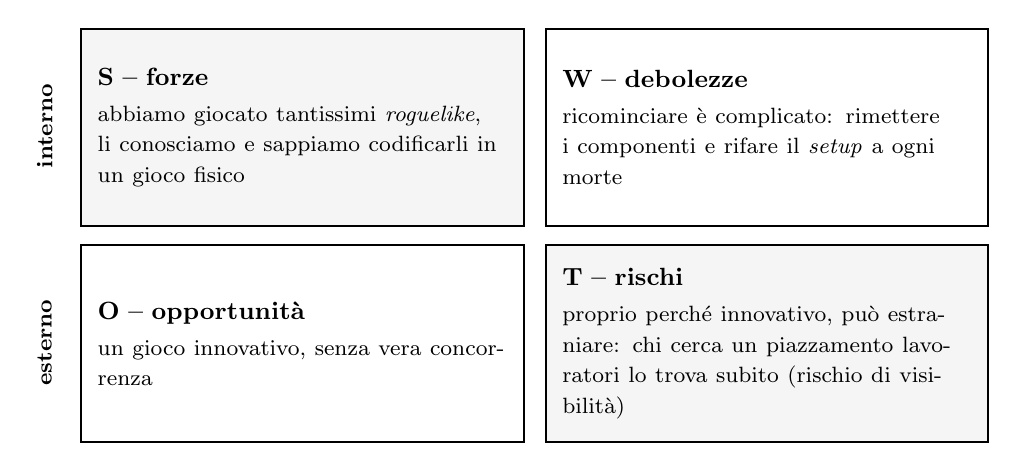
\begin{tikzpicture}[
  font=\small,
  a14q/.style={draw, thick, text width=5.2cm, minimum height=2.5cm, align=left,
               inner sep=6pt, anchor=north west}
]
  \node[a14q, fill=gray!8] (S) at (0,0) {\textbf{S -- forze}\\[2pt]\footnotesize abbiamo
    giocato tantissimi \emph{roguelike}, li conosciamo e sappiamo codificarli in un gioco
    fisico};
  \node[a14q] (W) at (5.9,0) {\textbf{W -- debolezze}\\[2pt]\footnotesize ricominciare è
    complicato: rimettere i componenti e rifare il \emph{setup} a ogni morte};
  \node[a14q] (O) at (0,-2.75) {\textbf{O -- opportunità}\\[2pt]\footnotesize un gioco
    innovativo, senza vera concorrenza};
  \node[a14q, fill=gray!8] (T) at (5.9,-2.75) {\textbf{T -- rischi}\\[2pt]\footnotesize
    proprio perché innovativo, può estraniare: chi cerca un piazzamento lavoratori lo
    trova subito (rischio di visibilità)};
  \node[rotate=90, font=\footnotesize\bfseries] at (-0.45,-1.25) {interno};
  \node[rotate=90, font=\footnotesize\bfseries] at (-0.45,-4.0) {esterno};
\end{tikzpicture}
\caption{L'analisi SWOT ``fatta in 30 secondi'' da Marta sull'esempio di un
\emph{roguelike} da tavolo. La riga in alto riguarda il progetto, quella in basso il mercato
di riferimento, inteso in senso largo (anche le persone che consultano itch.io). Le
categorie si leggono poi a coppie.}
\label{a14:fig:swot}
\end{figure}

\paragraph{Uno strumento si impara usandolo.} Ogni strumento visto oggi diventa più utile
\textbf{quanto più spesso lo si usa}. ``Non so se vi dilettate in cucina'', ma ci sono
tantissimi strumenti per cucinare, e più si usa uno strumento, più se ne conoscono limiti e
forze. Vale anche per la SWOT: ``la prima volta che la farete sarà una roba un po'
posticcia''; poi, man mano che la si sfrutta, si scoprono le sue utilità, soprattutto nel
\textbf{riassumere in breve} questi quattro punti.

% ---------------------------------------------------------------------
\section{Le \emph{personas}}
\label{a14:sec:personas}

\slidefig{img/AGD/agd14-personas}{Un esempio di persona.}{slide \emph{Tecniche di sviluppo}}{fig:agd14-personas}


Un altro strumento ``molto utile, sempre un po' mutuato da altri campi'', sono le
\textbf{\emph{personas}}, già accennate parlando di \emph{target}. ``Queste le conoscete?''
``Di nome, ma meno.''

\paragraph{Dal \emph{target} a una persona.} Quando si fa un gioco si ha in mente un
\emph{target}, ma i \emph{target} sono \textbf{misure astratte}: si può dire che un gioco è
``per gli appassionati'', ma ``se io dico appassionati, non ho in mente una persona''. Aiuta
invece avere \textbf{riferimenti molto specifici}. Siccome è difficile pensare in concreto a
una persona precisa che vuole il nostro gioco, si può ricorrere alle \emph{personas}, che
sono ``niente di più che'' \textbf{profili creati da noi}, popolati il più possibile.
Generalmente si costruiscono partendo da \textbf{dati molto generici} e poi
\textbf{scendendo nei dettagli}, stabilendo sempre di più i tratti di questa persona virtuale.

\paragraph{L'esempio della slide.} Nell'esempio della slide non c'è niente che non sia
definito in modo certo: la persona ha un \textbf{nome}\footnote{Nella trascrizione il nome è
prima ``Tian'' e poi ``Diane''; l'occupazione è ``e share consultant'', forse \emph{HR
consultant}. La slide non è nella trascrizione e il capitolo non può verificarlo.},
un'\textbf{età} (48 anni), un'\textbf{occupazione} (una consulente) e una \textbf{biografia},
una \emph{backstory} che racconta le cose che fa ogni giorno. Che cosa c'entrano con un gioco
da tavolo? ``Tendenzialmente, di base, niente.'' Ma anche per una persona reale le cose che fa
nella vita c'entrano poco con i suoi hobby; eppure ci aiutano a immaginare \textbf{che cosa
farebbe quella persona seduta a un tavolo da gioco}. Costruire una \emph{persona} dà una
dimensione e permette di \textbf{rispondere a delle domande}, del tipo: ``Diane giocherebbe
a \emph{I Coloni di Catan}?''\footnote{Nella trascrizione ``colonie di Katan''.} Più la
\emph{persona} è definita, più è probabile riuscire a rispondere.

\paragraph{Il rischio dei \emph{bias}.} Per la SWOT come per le \emph{personas}, il rischio è
che \textbf{i propri \emph{bias} condizionino il lavoro}. ``È un rischio che c'è sempre.''
L'invito è a essere persone \textbf{aperte} il più possibile, \textbf{curiose}, e a
\textbf{conoscere più persone possibile}: dà un vantaggio, e aiuta a calarsi negli altri con
più facilità.

\paragraph{\emph{Personas} costruite sui dati.} A seconda dell'entità del progetto, si possono
\textbf{raccogliere dei dati} e costruire le \emph{personas} su quei dati: fare dei campioni
quantitativi, per esempio con \textbf{un sondaggio}, per capire abitudini diffuse e interessi
condivisi di un certo \emph{target}. ``Magari a volte vi è capitato di fare un sondaggio'' che
chiedeva ``sei appassionata di giochi da tavolo?'' e poi ``quali libri leggi?'': ``e tu dici:
ok, ma che c'entra?''. A volte serve proprio a costruire questi profili.

\paragraph{Riusarle o no?} Uno degli inviti che si leggono spesso è a \textbf{non usare le
stesse \emph{personas} per più di un progetto}. Marta non la trova una regola necessariamente
funzionale: le è capitato di riusare le stesse \emph{personas} per più progetti, ``e
sinceramente non capisco bene il perché di no''. Riporta comunque quello che ha letto quando
ha imparato la tecnica: ognuno veda se gli torna utile.

\paragraph{Approfondimento: \emph{personas} e modelli di pubblico.} Bateman e Boon partono da
un modello di pubblico ancora più grezzo di quello che Marta chiama ``gli appassionati'': la
divisione tra giocatori \emph{hardcore} e \emph{casual}, che definiscono una ``ipotesi
consensuale'', accettata da quasi tutti nell'industria ma senza una definizione formale. Il
loro esempio è \emph{Resident Evil} per GameCube, che all'inizio chiedeva al giocatore se
preferisse ``scalare la montagna'' (oltre le fatiche c'è il risultato) o ``fare
un'escursione'' (la meta si raggiunge comodamente), per regolare la difficoltà. Le
\emph{personas} fanno il passo successivo: invece di due etichette, una persona con un nome,
un'età e una giornata, a cui fare domande concrete.

% ---------------------------------------------------------------------
\section{I sei cappelli per pensare}
\label{a14:sec:cappelli}

\slidefig{img/AGD/agd14-cappelli}{I sei cappelli per pensare.}{slide \emph{Tecniche di sviluppo}}{fig:agd14-cappelli}


``I sei cappelli per pensare. Questa forse la conoscete anche dal \emph{design}''. Qualcuno
l'ha sentita nominare; una voce, probabilmente di una studentessa, ricorda che nei suoi studi di \emph{design} se ne
parlava, ``ma non tramite i cappelli colorati'': il processo creativo analizzato da altri
punti di vista, ``però è molto interessante anche così''.

\paragraph{La prima pausa.} A questo punto Marta resta bloccata fuori dalle slide: ha aperto
la chat di Zoom e non riesce più a tornare alla presentazione (``vi giuro che non sono mai
stata così in difficoltà'', ``ho anche una laurea in informatica''; ``e ho fatto l'errore di
aprire la chat, non lo farò mai più''). Gli studenti continuano a vedere le slide, ma lei non
riesce a farle avanzare, e propone \textbf{dieci minuti di pausa} per risolvere. La pausa,
nella trascrizione, è coperta da frasi ripetute senza senso. Al ritorno: ``nel frattempo ho
trovato il modo di aprire la chat senza distruggere mezzo computer''.

\paragraph{A che cosa servono.} I sei cappelli sono un altro dei processi per
\textbf{calarsi in panni che non sono i propri}, utili soprattutto per figurarsi prospettive
che non sono quelle che vengono ``di primo acchito'' quando si lavora a un progetto. I
cappelli guardano a problemi simili \textbf{da punti di vista diversi}, e alcuni sono
volutamente \textbf{opposti}. Si possono usare in molti modi; Marta, per esempio, ha
\textbf{un mazzetto di sei carte}: le mescola, ne estrae una e si mette figurativamente quel
cappello. Si possono usare anche \textbf{in \emph{team}}: ognuno indossa un cappello, e poi
i cappelli \textbf{ruotano} per cambiare punto di vista. La tabella~\ref{a14:tab:cappelli}
li riassume.

\begin{description}
  \item[Il bianco: i fatti.] Guarda le cose \textbf{da un punto di vista neutrale}: asserisce
        i fatti nel modo più oggettivo possibile, si astiene dai giudizi e dà informazioni
        ``il più possibile dritte''. Per esempio: ``durante il \emph{playtest} è successa
        questa cosa'', senza dire se è positiva o negativa; ``si è verificato un paio di
        volte questo avvenimento''. Prende i dati in modo \textbf{distaccato}.
  \item[Il nero: i rischi.] Fa leva su \textbf{difficoltà, insicurezze, pericoli}: tutto
        quello che potrebbe non essere andato o potrebbe non andare. È uno dei cappelli
        \textbf{più facili da indossare}, perché è facile vedere le parti negative di un
        progetto. Proprio per questo invita a essere \textbf{più descrittivi}: non limitarsi
        a dire qual è la difficoltà, ma esplorarla e analizzarla nel dettaglio.
  \item[Il rosso: le emozioni.] Fa riferimento alle \textbf{emozioni}: come ci si sente
        quando lo si indossa, quali emozioni sono state provate. A differenza del nero,
        \textbf{non dà spiegazioni}: dice ``io mi sento così''. È un cappello molto utile e
        \textbf{spesso sottovalutato}, perché c'è la credenza che le emozioni valgano meno
        dei fatti; in realtà le emozioni guidano a capire qual è \textbf{l'esperienza
        desiderata}, che cosa si vuole ottenere da un \emph{design}, e se il \emph{design} lo
        sta facendo emergere.
  \item[Il giallo: i punti di forza.] È l'opposto del nero: elenca \textbf{le cose positive},
        i punti di forza, gli aspetti che esaltano l'esperienza. Anche questo è abbastanza
        semplice da indossare; anche qui l'invito è a ``lasciarsi andare'' sulle
        \textbf{ragioni} per cui quei punti sono di forza, e a sviscerarle.
  \item[La creatività.] Uno dei due cappelli ``più particolari''\footnote{Marta non dice il
        colore di questo cappello. Nel metodo originale di Edward de Bono (\emph{Six Thinking
        Hats}, 1985) il cappello della creatività è il \textbf{verde}.}: significa
        \textbf{lanciarsi in soluzioni anche esagerate e irrealistiche}. È il cappello del
        \textbf{\emph{brainstorming}}: si analizzano le possibilità, anche quelle fuori dagli
        schemi. Non importa se sono fattibili: il lavoro della creatività è \textbf{proporre
        idee}, soluzioni, possibilità; pensare a quali e quante sono, e cercare quelle più
        inusuali.
  \item[Il blu: l'organizzazione.] Il più particolare. In \emph{team} serve a
        \textbf{gestire gli altri cappelli}: chi indossa il blu stabilisce quando si cambia
        cappello. E inoltre dice: ``ok, però che cosa faremo? Che cosa implementeremo? Che
        cosa serve adesso per raggiungere gli scopi che ci prefiggiamo?''. È la parte
        \textbf{organizzativa} del processo, quella che segue la parte pratica una volta
        individuate le caratteristiche.
\end{description}

Nel complesso, i cappelli sono anche un modo di \textbf{dividere i pensieri in compartimenti
stagni}, ``e a volte questa cosa torna particolarmente utile''.

\begin{table}[htbp]
\centering
\small
\begin{tabular}{@{}p{2.3cm}p{3.6cm}p{3.9cm}p{3.7cm}@{}}
\toprule
\textbf{Cappello} & \textbf{Guarda a} & \textbf{Esempio di frase} & \textbf{Attenzione} \\
\midrule
Bianco & i fatti, neutri & ``durante il \emph{playtest} è successo due volte X'' & niente
  giudizi \\
\addlinespace
Nero & difficoltà, insicurezze, pericoli & ``questo potrebbe non funzionare perché\ldots'' &
  facile da indossare: va approfondito \\
\addlinespace
Rosso & le emozioni & ``io mi sento così'' & niente spiegazioni; spesso sottovalutato \\
\addlinespace
Giallo & i punti di forza & ``questo esalta l'esperienza perché\ldots'' & facile: andare a
  fondo delle ragioni \\
\addlinespace
Creatività (verde) & idee e soluzioni, anche irrealistiche & ``e se\ldots?'' & non giudica
  la fattibilità \\
\addlinespace
Blu & l'organizzazione: quando cambiare, che cosa fare ora & ``che cosa implementiamo?'' &
  in \emph{team}, gestisce gli altri \\
\bottomrule
\end{tabular}
\caption{I sei cappelli per pensare come li presenta Marta. Si possono pescare da un mazzetto
di sei carte, da soli, o far ruotare in un \emph{team}.}
\label{a14:tab:cappelli}
\end{table}

% ---------------------------------------------------------------------
\section{Il bilanciamento secondo Garfield}
\label{a14:sec:garfield}

\slidefig{img/AGD/agd14-bilancia}{Il bilanciamento.}{slide \emph{Tecniche di sviluppo}}{fig:agd14-bilancia}


``Ecco, ce l'ho fatta'': la slide successiva è il \textbf{bilanciamento}. ``Questo è il capitolo
un po' più complicato da fare, ma vedremo perché.'' Marta raccomanda di interromperla con le
domande, perché è ``un argomento molto spesso spinoso'', e lei lo tratta ``in un modo un po'
atipico rispetto ai miei colleghi''.

\paragraph{\emph{The Balancing Act}.} Si parte da uno degli articoli che da qualche anno sono
diventati un punto di riferimento per il suo lavoro, scritto ``niente di meno che'' da
\textbf{Richard Garfield}\footnote{Marta cita il titolo dell'articolo, \emph{The Balancing
Act}, ma non dice dove sia stato pubblicato; il capitolo non lo ha verificato. Le citazioni
che seguono sono la parafrasi italiana di Marta dalla slide, non il testo originale.}. Lo si
troverà citato spesso: Garfield è un designer con un'esperienza ormai
\textbf{quarantennale} (``ormai sono 40 anni, direi''), con tantissimi giochi di successo,
``non c'è solo \emph{Magic}'', e ha una profonda conoscenza non solo del gioco ma di tutto
ciò che gli ruota attorno. ``Secondo me è un'ottima lettura a prescindere'': molto spesso è
stato \textbf{sottovalutato}, perché molti lo associano solo a \emph{Magic}, ``e invece ha
fatto tanto, tanto di più''. Nell'articolo Garfield esorta così:
\begin{quote}
\textbf{il bilanciamento perfetto dei giochi è un mito. Il bilanciamento consiste nel
migliorare il \emph{play}, il giocare, per un ampio spettro di possibili giocatori, e
comporta costi e benefici.}
\end{quote}
È una frase che, per Marta, riassume perfettamente tanti punti del bilanciamento. La parte che
molti dimenticano è quella dei \textbf{costi e benefici}: qualsiasi bilanciamento si operi
presenterà, ``se vogliamo, anche per ricondurci all'analisi SWOT'', delle forze, delle
debolezze, delle opportunità e dei rischi.

\paragraph{Un'esplorazione dello spazio di gioco.} Che cos'è, allora, il bilanciamento? Si
può definire come \textbf{l'esplorazione di una parte dello spazio di gioco totale}. Dato un
gioco, applicando bilanciamenti diversi, e anche regole diverse, se ne esplora una parte
diversa. Quando si presenta un gioco sviluppato, finito, si sta implicitamente consegnando
\textbf{una porzione di uno spazio di gioco molto più ampio} (figura~\ref{a14:fig:spazio}).

\paragraph{Non esiste un bilanciamento che accontenti tutti.} Si pensa che questa porzione
debba accontentare tutti, ma, proprio per i costi e benefici, non è così. Molto spesso chi
segue il principio di accontentare tutti \textbf{sta accontentando soltanto la parte più
rumorosa dell'utenza}: quella che si esprime in modo più vocale, spesso non da una posizione
di conoscenza, ma perché è molto facile giudicare un gioco; e ``quindi molto spesso si
prendono dei granchi''. \textbf{Abbandonare l'idea che un gioco possa risultare adatto a
chiunque} è, per Marta, l'obiettivo da avere quando ci si mette sotto con lo sviluppo: ``non
esistono giochi che sono adatti a tutte le persone''.

\begin{figure}[htbp]
\centering
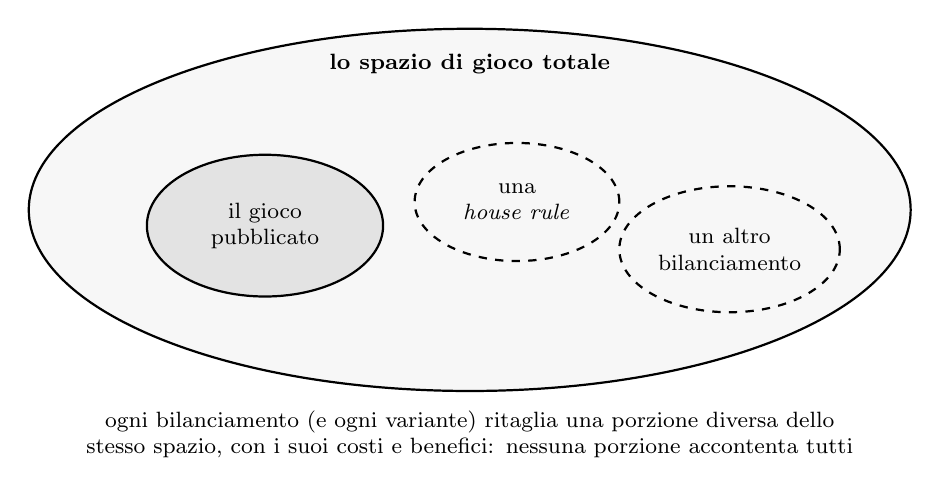
\begin{tikzpicture}[font=\small]
  \draw[thick, fill=gray!6] (0,0) ellipse (5.6cm and 2.3cm);
  \node[font=\footnotesize\bfseries] at (0,1.85) {lo spazio di gioco totale};
  \draw[thick, fill=gray!22] (-2.6,-0.2) ellipse (1.5cm and 0.9cm);
  \node[align=center, font=\footnotesize] at (-2.6,-0.2) {il gioco\\pubblicato};
  \draw[thick, dashed] (0.6,0.1) ellipse (1.3cm and 0.75cm);
  \node[align=center, font=\footnotesize] at (0.6,0.1) {una\\\emph{house rule}};
  \draw[thick, dashed] (3.3,-0.5) ellipse (1.4cm and 0.8cm);
  \node[align=center, font=\footnotesize] at (3.3,-0.5) {un altro\\bilanciamento};
  \node[font=\footnotesize, text width=10cm, align=center] at (0,-2.85) {ogni bilanciamento
    (e ogni variante) ritaglia una porzione diversa dello stesso spazio, con i suoi costi e
    benefici: nessuna porzione accontenta tutti};
\end{tikzpicture}
\caption{Il bilanciamento come esplorazione dello spazio di gioco: il gioco finito ne
consegna una porzione; le \emph{house rules} e le varianti, nell'analogico, permettono a chi
gioca di esplorarne altre.}
\label{a14:fig:spazio}
\end{figure}

\paragraph{Dare più potere a chi gioca.} Il mondo analogico ha una grande forza che nel
videogioco non è altrettanto facile: \textbf{se vogliamo cambiare una regola, basta dirlo
quando si spiegano le regole}. Nel videogioco, per farlo, servono di solito conoscenze di
programmazione o di progettazione che vanno al di là di quello che l'utenza comune riesce a
fare. Il gioco analogico dà invece uno strumento molto forte: \textbf{varianti} e
\textbf{\emph{house rules}}, per tarare il gioco sul proprio livello.

\paragraph{Il gioco non è un artefatto immutabile.} Marta spende ``altre due parole''. C'è una
tendenza, che lei stessa ha seguito per tanti anni, a pensare al gioco come a un
\textbf{artefatto immutabile}: è stato fatto così e non può essere toccato. Esiste in molti
ambiti, per esempio con i libri, che molte persone non vogliono assolutamente modificare,
segnare, sottolineare. È una concezione che Marta si prende la libertà di definire ``molto
orientata al capitalismo'', in cui gli oggetti non sono davvero propri ma entità da
preservare per preservarne il valore. I \textbf{giochi \emph{legacy}} aiutano a svincolarsi
da questo principio. \textbf{Lavorare su un gioco e metterci del proprio è il gesto di
possesso più forte che si possa fare}, e in un certo senso anche un gesto d'amore: se si
modifica un gioco con \emph{house rules} e varianti, probabilmente è perché piace così tanto
che, piuttosto che bollarlo come ``non è un gioco per me'', si è disposti a
\textbf{esplorarne lo spazio di gioco}. È una cosa che nell'ambiente si è un po' persa, ma
che è sempre stata una caratteristica del gioco: Marta invita a riscoprirla, ``perché tira
fuori tante cose positive''.

\paragraph{Le \emph{house rules} come palestra di sviluppo.} Inoltre, praticare le \emph{house
rules} \textbf{spinge verso lo sviluppo}: toccare un gioco edito e vedere come cambia variando
le regole trasmette il \emph{feeling} di lavorare a un gioco già creato da qualcun altro e
metterci le mani sopra, cioè proprio il mestiere di chi sviluppa.

\paragraph{L'obiettivo: esaltare le forze, minimizzare gli ostacoli.} L'obiettivo del
bilanciamento è lo stesso dello sviluppo in generale: \textbf{esaltare le forze del
\emph{design} e minimizzare gli ostacoli}. Non lo si pensi come il raggiungimento di un
\textbf{equilibrio perfetto}, che non esiste; ci si chieda sempre: ``ok, però questo
\emph{design} che cosa si promette di fare? Come faccio a veicolarlo?''.

% ---------------------------------------------------------------------
\section{Per chi si bilancia}
\label{a14:sec:perchi}

È importante ricordare \textbf{per chi} si sta facendo il bilanciamento. Potrebbero essere
persone \textbf{esperte}, appassionate; persone \textbf{alle prime armi}; o, a volte, ``il
\textbf{dio della simmetria}'', come lo chiamano dove lavora Marta.

\paragraph{Il dio della simmetria.} È quando ci si intestardisce che \textbf{i numeri debbano
finire tutti per 5 o per 10}, o che, siccome questa carta vale 2, \textbf{anche quella debba
valere 2}, senza contemplare per esempio i numeri dispari: ``sono tutte delle fisime che vengono
fuori quando si sviluppa''\footnote{Nella trascrizione ``sono tutte delle fisiche'': quasi
certamente ``fisime''.}. ``Io sono la prima che a volte ci cade, in questi tranelli'': l'ha
messo nella slide anche per prendersi in giro. Ma è un avvertimento serio: quando si bilancia,
si tende verso i propri \emph{bias}, e il dio della simmetria è uno di questi.

\paragraph{Bilanciare per il gioco.} A volte si bilancia \textbf{per il gioco}, cioè per il suo
interesse: il gioco vuole creare certe dinamiche, quelle infuse da chi l'ha creato, e
bilanciare per il gioco significa \textbf{non pensare necessariamente al \emph{target}}, ma a
come tirare fuori il più possibile l'esperienza. Vale soprattutto per i \textbf{giochi non
commerciali}, in cui l'interesse è portare l'esperienza anche a discapito dell'utenza, e per
i giochi \textbf{molto sperimentali}.

L'esempio è un gioco ``molto bello'' di \textbf{Amabel Holland}, in solitario, che si chiama
\textbf{\emph{Endurance}}\footnote{Il titolo e l'autrice sono detti chiaramente; editore e
anno non sono nominati. Amabel Holland pubblica di solito con Hollandspiele.}. Ricrea le
vicende della spedizione dell'\emph{Endurance}, ``una spedizione miracolosa'' in cui i membri
dell'equipaggio si sono salvati dopo una quantità immensa di tempo passato, ``se non
sbaglio'', in Antartide\footnote{È la spedizione imperiale transantartica di Ernest
Shackleton (1914--1917): la nave \emph{Endurance} rimase intrappolata nei ghiacci e affondò,
e tutto l'equipaggio sopravvisse dopo quasi due anni.}. Quello che Holland ha voluto ricreare
è che, quando si gioca, \textbf{nel 99\% dei casi si perde}, perché l'equipaggio muore.
``Perdere'' è un'imprecisione: nel gioco \textbf{non ci sono vere condizioni di vittoria o di
sconfitta}, ma un'analisi di quello che è successo e un racconto dell'esperienza. La storia in
cui tutti si salvano è \textbf{volutamente rarissima}, per dimostrare la straordinarietà
dell'evento reale e ricalcare la difficoltà di ottenere un risultato del genere. Qui si
bilancia per il gioco, anche se il \emph{target} potrebbe non apprezzarlo; o meglio, c'è un
\emph{target} ``un po' più nascosto'' di quello commerciale.

\paragraph{Bilanciare per il \emph{target}.} È il discorso inverso: si bilancia per chi,
secondo noi, giocherà il gioco. Tendenzialmente si bilancia per il \emph{target}, ma nella
pratica è più difficile di quanto sembri, perché è facile \textbf{dimenticare che si sta
bilanciando per persone con interessi diversi dai nostri}, e finire a bilanciare per noi
stessi. L'esempio che aiuta è quello dei \textbf{giochi per bambini}: lì ``chiaramente noi non
siamo bambini'', e la differenza salta all'occhio. Quando Marta ha lavorato a un gioco per
bambini chiamato \textbf{\emph{Sun Farm}}\footnote{Così nella trascrizione; il titolo non è
verificabile.}, il bilanciamento è partito \textbf{dai bambini e dai genitori}: capire quale
potesse essere l'esperienza desiderata da un bambino, e perché in quel caso \textbf{vincere
non era la cosa più importante dell'universo}, mentre contavano di più
l'\textbf{espressività} e la possibilità di giocare un po' con le strategie senza restringere
il campo delle possibilità.

\paragraph{Esperti o principianti.} C'è spesso la tendenza a fare giochi \textbf{solo per i
giocatori migliori}, o per quelli che sono vocali e si spacciano per i migliori. Molto spesso
sono persone che \textbf{il gioco l'hanno giocato pochissimo}: sui gruppi e sui \emph{forum}
si trovano persone che dicono ``questo gioco è rotto'' dopo una partita. È una tendenza che
c'è anche \textbf{nell'industria}, dietro le quinte, tra addetti ai lavori; ``posso ammettere
che anche io l'ho fatto''. Ed è, come dice anche Garfield, \textbf{profondamente
irrispettoso}: si pensa che il gioco sia fatto solo per noi, quando magari non siamo
minimamente nel suo \emph{target}, o il gioco richiede competenze che non abbiamo o non
abbiamo voglia di applicare. Bisogna ricordarsi che \textbf{un gioco non è giocato soltanto
da queste persone}: è giocato da tantissime persone che non commentano sui \emph{forum}, non
scrivono su BGG, non lasciano voti. E il gioco deve essere \textbf{accessibile al maggior
numero possibile di persone}, proprio perché arrivi anche nelle mani di chi non si esprime ma
avrebbe piacere di giocarlo.

\paragraph{Tecnicità contro approcciabilità.} Per riassumere: da una parte si bilancia
\textbf{per tecnicità}, per rendere il gioco ``più bello'', e magari non si riesce ad
accontentare nessuno, perché per $N$ persone che si lamentano ce ne saranno $M$ che si
lamenteranno una volta fatta la modifica. Dall'altra si bilancia \textbf{per
approcciabilità}, per rendere il gioco più approcciabile: questo \textbf{allarga la base
d'utenza} che può accedere al gioco e favorisce che venga effettivamente provato. Marta
precisa, ``fatemi sapere se non vi è chiara la differenza'': \textbf{non significa che non si
possano fare giochi complessi}, o impegnativi. ``Non è questo il punto del discorso.''

% ---------------------------------------------------------------------
\section{Perché non bilanciare (solo) con la matematica}
\label{a14:sec:matematica}

Perché, allora, non si bilancia spesso \textbf{``in modo matematico''}, come si dice? Marta
elenca le ragioni.

\paragraph{È lungo e soggetto a errori.} Non conosce le competenze matematiche di tutte le
persone che si avvicinano al \emph{design} e allo sviluppo, ma nella sua esperienza vede
molto spesso \textbf{ragionamenti matematici fallaci}, che ``non stanno in piedi''. Ed è un
processo \textbf{lungo e faticoso}, che porta a sbagliare tantissime volte. A meno di essere
``davvero, davvero, davvero molto in gamba'' su questo aspetto, va affrontato con cautela.

\paragraph{È difficilmente modellabile.} Molto spesso \textbf{i modelli sono sbagliati}:
quando si cerca di sintetizzare un gioco si perdono \textbf{le dipendenze tra le risorse}, le
\textbf{transazioni} da una risorsa all'altra, da una carta all'altra. E si perde quello che
rende i giochi affascinanti: i cosiddetti \textbf{spazi di permeabilità}, già nominati
``ieri'', che \textbf{neanche il designer conosce sempre in modo approfondito} e che fanno la
differenza. I giochi sono interessanti proprio perché sono sistemi \textbf{non pienamente
controllati, non pienamente compresi}. Si pensi agli \textbf{scacchi}: chi li ha progettati
non aveva ``minimamente idea'' di tutto quello che è venuto dopo; molte innovazioni
strategiche sono degli ultimi cinquant'anni. È notevole quanti spazi di permeabilità avesse,
grazie alla struttura aperta del suo albero decisionale, ``che, penso lo sapete, è
immenso''.

\paragraph{Appiattisce le scelte.} Bilanciare in modo matematico porta a un
\textbf{appiattimento delle scelte}, perché si tende a trovare degli \textbf{equilibri
statici}: si immagini una bilancia perfettamente in equilibrio. Ne nascono le famose
\textbf{scelte indifferenti}: qualsiasi cosa si faccia, la ricompensa è identica. Un percorso
dà 1 punto vittoria al primo turno, 3 al secondo e 2 al terzo; un altro ne dà 1 al primo, 2 al
secondo e 3 al terzo. Alla fine \textbf{sono 6 punti per tutte e due le strade}: ``quindi
abbiamo risolto assolutamente niente'' (figura~\ref{a14:fig:indifferenti}). L'esperienza
diventa \textbf{statica e priva di significato}.

\begin{figure}[htbp]
\centering
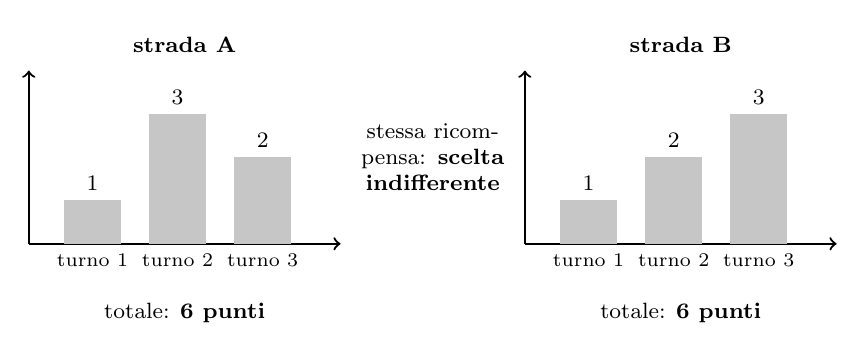
\begin{tikzpicture}[font=\small, x=0.9cm, y=0.55cm]
  % assi
  \foreach \ox/\tit/\a/\b/\c in {0/{strada A}/1/3/2, 7/{strada B}/1/2/3}{
    \draw[thick, ->] (\ox,0) -- (\ox+4.4,0);
    \draw[thick, ->] (\ox,0) -- (\ox,4.0);
    \node[font=\footnotesize\bfseries] at (\ox+2.2,4.6) {\tit};
    \fill[gray!45] (\ox+0.5,0) rectangle (\ox+1.3,\a);
    \fill[gray!45] (\ox+1.7,0) rectangle (\ox+2.5,\b);
    \fill[gray!45] (\ox+2.9,0) rectangle (\ox+3.7,\c);
    \node[font=\footnotesize, above] at (\ox+0.9,\a) {\a};
    \node[font=\footnotesize, above] at (\ox+2.1,\b) {\b};
    \node[font=\footnotesize, above] at (\ox+3.3,\c) {\c};
    \node[font=\scriptsize, below] at (\ox+0.9,0) {turno 1};
    \node[font=\scriptsize, below] at (\ox+2.1,0) {turno 2};
    \node[font=\scriptsize, below] at (\ox+3.3,0) {turno 3};
    \node[font=\footnotesize] at (\ox+2.2,-1.6) {totale: \textbf{6 punti}};
  }
  \node[font=\footnotesize, text width=2.4cm, align=center] at (5.7,2.0) {stessa
    ricompensa: \textbf{scelta indifferente}};
\end{tikzpicture}
\caption{L'esempio di Marta di scelte indifferenti, prodotto da un bilanciamento matematico
``statico'': due percorsi con andamenti diversi ma lo stesso totale. Scegliere l'uno o
l'altro non cambia niente.}
\label{a14:fig:indifferenti}
\end{figure}

``Anche qua'', precisa, ``non significa che non si usa la matematica'': la matematica aiuta e
può tornare comoda sotto molti aspetti. Ma bisogna fare attenzione a \textbf{non guardare il
bilanciamento solo da questo punto di vista}, perché è una tendenza comune a chi si avvicina al
bilanciamento e porta a degli errori.

\paragraph{Il bilanciamento esperienziale.} Marta consiglia sempre il \textbf{bilanciamento
esperienziale}: veicolare \textbf{i percorsi intesi}, l'obiettivo del \emph{design}. Che cosa
si prefigge il gioco? Quali strade voglio che siano percorse a livello strategico? Che cosa
voglio \textbf{premiare}? Costruire le \textbf{scelte sensibili}, cioè indirizzare le scelte
delle persone verso alcune delle idee e delle strategie che si vogliono mettere in campo, e
lasciare che il \emph{gameplay} sia \textbf{emergente}, che consenta anche a chi gioca di
metterci del proprio. Il bilanciamento esperienziale è anche \textbf{parametrizzabile}: se tra
gli \emph{stakeholder} c'è chi vuole un gioco ``un po' più cattivo'', che restituisca un
\emph{feeling} di frustrazione, lo si può fare senza problemi; il bilanciamento matematico
molto spesso lo impedisce, perché tende a equalizzare tutto su un livello statico.

\paragraph{E l'intelligenza artificiale?} Un tema diventato rilevante quest'anno, ``l'anno
scorso lo era un po' meno'': molte persone \textbf{bilanciano con l'intelligenza
artificiale}. Marta non si mette a spiegare come funziona, ``però insomma, non è una cosa che
veramente pensi, mettiamola così: è semplicemente un \textbf{algoritmo predittivo}''. Molto
spesso porta proprio agli \textbf{errori del bilanciamento matematico}. Il suo invito è a
\textbf{non usarla}; ma chi la usa faccia attenzione, perché può portare a un bilanciamento
``assolutamente errato e che appiattisce il gioco''.

\paragraph{Approfondimento: il modello e il gioco.} Schell non è contrario ai modelli, ma ne
descrive bene il limite: ``il modello informa il bilanciamento, e il bilanciamento informa il
modello''. Si scrive il proprio modello di come sono legate le meccaniche, lo si mette alla
prova giocando, e lo si corregge ogni volta che il gioco non si comporta come previsto.
Aggiunge che il bilanciamento può cominciare davvero solo quando il gioco è giocabile, e che
la sua regola personale è dedicare al bilanciamento \textbf{metà del tempo di sviluppo}. È la
stessa direzione di Marta: i numeri servono, ma come ipotesi da verificare al tavolo, non come
risposta.

% ---------------------------------------------------------------------
\section{Come cominciare: giochi a scarsa interazione}
\label{a14:sec:cominciare}

Un consiglio per chi vuole iniziare a sperimentare con il bilanciamento: partire da
\textbf{giochi a scarsa interazione}. I giochi ad alta interazione hanno tante
\textbf{interdipendenze} con quello che fanno i giocatori; si possono modellare anche
matematicamente, soprattutto in termini probabilistici, ``ma è molto complesso''. Partire da
giochi con poca interazione permette di lavorare in modo più agevole. Marta precisa che sta
parlando soprattutto di giochi con \textbf{un modello matematico alle spalle}: giochi con
\textbf{conversioni di risorse}, in cui si vince a \textbf{punti vittoria}; non tanto di giochi
narrativi. Nel mondo del gioco da tavolo c'è ancora una preponderanza di questo tipo di giochi,
e quando si parla di bilanciamento si parla di solito di questo, anche se, come detto la volta
prima, non è affatto l'unico che si fa.

\paragraph{Modellare il sistema.} Partendo da un gioco a scarsa interazione, si prova a
\textbf{modellarne il sistema}: capire le \textbf{dipendenze} tra le risorse, con un
\textbf{diagramma di flusso} o anche un \textbf{diagramma di stato}, se torna utile.
L'obiettivo è individuare il \textbf{percorso che fanno le risorse}: quando vengono prese,
quando vengono restituite, e così via.

\paragraph{Un esempio: \emph{Splendor} infinito.} Si può partire da \textbf{\emph{Splendor}} e
immaginarlo con \textbf{risorse infinite}: le fiche di ogni colore sono infinite, e le carte
sono in $N$ copie, quindi possono essere sempre prese. Si prova a bilanciare da lì e si vede
che succede.

\paragraph{Variare i parametri.} Si testa come varia il gioco al variare dei parametri,
semplicemente \textbf{cambiando i parametri}, anche in modo arbitrario (tra poco si vedranno
alcune tecniche). Per esempio: che succede se, in \emph{Splendor}, una delle risorse, la
carta, diventa \textbf{esclusiva}, e non più in $N$ copie?

\paragraph{I \emph{test} in solitaria e il \emph{groupthink}.} I \emph{test} in solitaria qui
sono agevoli, ma attenzione al \textbf{\emph{groupthink}}, soprattutto se se ne fanno molti
durante il bilanciamento: ragionando da soli capita molto spesso di \textbf{rinforzare i
propri \emph{bias}}, e può diventare un problema, soprattutto se non si è consapevoli di
averli. Bisogna testare con \textbf{più persone}, e potenzialmente con \textbf{più gruppi
possibili}, per capire come si assesta il bilanciamento ed evitare il fenomeno.

\paragraph{Lasciare gli spazi di permeabilità.} ``Mi raccomando'': non bisogna avere
\textbf{l'ansia di controllare tutto il sistema di gioco}; non è necessario.

\paragraph{La strategia dominante emerge.} Se c'è una \textbf{strategia dominante}, di solito
la si intuisce analizzando il gioco da diversi punti di vista, o anche banalmente con i
\emph{playtest}: con un numero sufficiente di partite, i comportamenti emergono. L'esempio più
popolare: \textbf{tenere traccia di chi inizia a giocare} e vedere se è la persona che vince.
Se lo è, c'è un problema: chi inizia magari vince perché \textbf{fa un turno in più} degli
altri (``generalmente questo può essere uno dei motivi'').

% ---------------------------------------------------------------------
\section{Il budget di complessità}
\label{a14:sec:budget}

Uno dei concetti che tornano molto utili nello sviluppo, e che si trovano spesso soprattutto
nel bilanciamento, è il \textbf{budget di complessità}. Un gioco ha una certa complessità, un
certo grado di difficoltà: non la si immagini necessariamente come un numero, ma comunque come
\textbf{una quantità}, una quantità $x$. Quando si lavora al gioco, \textbf{rimuovere o
cambiare delle parti altera il budget}. Generalmente, togliendo per esempio una meccanica, si
\textbf{guadagna} complessità disponibile. E che cosa ci si fa, con questo guadagno?
\begin{itemize}
  \item lo si può semplicemente \textbf{togliere}, riducendo la complessità generale
        dell'esperienza;
  \item oppure lo si può \textbf{investire} altrove.
\end{itemize}

\paragraph{L'esempio del mercato azionario.} Si immagini un gioco con un obiettivo molto
definito: far sperimentare a chi gioca \textbf{come varia il mercato azionario}. Sul tavolo ci
sono i vari beni messi sul mercato, e bisogna rappresentare questo aspetto. Se il gioco ha
anche una \textbf{fase d'asta}, sta concentrandosi sull'asta: oltre ad aggiungere complessità,
\textbf{toglie \emph{focus}} alle fluttuazioni di mercato, cioè al comprare e vendere.
Togliendo l'asta si riduce la complessità; e quello che si è guadagnato lo si può usare per
rendere \textbf{un po' più complessa} la parte del mercato: il comprare, il vendere, il variare
dei prezzi dei beni. Il gioco diventa \textbf{più focalizzato}, più centrato su ciò che vuole
rappresentare, al prezzo di aver tolto una meccanica, ma \textbf{senza aver necessariamente
ridotto il budget di complessità} (figura~\ref{a14:fig:budget}).

\paragraph{Nel dubbio, accessibile.} Se non si intuisce che c'è qualcosa da fare con la
complessità recuperata, ``chiaramente sappiate che è sempre meglio avere un gioco
\textbf{accessibile} laddove è possibile'': lo scoglio iniziale, cioè provare il gioco e
metterlo sul tavolo, diventa più semplice.

\begin{figure}[htbp]
\centering
\begin{tikzpicture}[font=\small, x=1cm, y=1cm]
  % prima
  \node[font=\footnotesize\bfseries] at (1.0,4.5) {prima};
  \draw[thick] (0,0) rectangle (2,4);
  \fill[gray!20] (0,0) rectangle (2,1.6);
  \node[font=\footnotesize] at (1,0.8) {asta};
  \fill[gray!45] (0,1.6) rectangle (2,3.6);
  \node[font=\footnotesize, align=center] at (1,2.6) {mercato};
  \node[font=\scriptsize] at (1,3.8) {altro};
  % opzione 1
  \node[font=\footnotesize\bfseries, align=center] at (5.2,4.5) {togliere e\\basta};
  \draw[thick] (4.2,0) rectangle (6.2,4);
  \fill[gray!45] (4.2,0) rectangle (6.2,2.0);
  \node[font=\footnotesize] at (5.2,1.0) {mercato};
  \node[font=\scriptsize] at (5.2,2.2) {altro};
  \node[font=\scriptsize, align=center] at (5.2,3.3) {budget\\libero};
  % opzione 2
  \node[font=\footnotesize\bfseries, align=center] at (9.4,4.5) {reinvestire\\nel focus};
  \draw[thick] (8.4,0) rectangle (10.4,4);
  \fill[gray!45] (8.4,0) rectangle (10.4,3.6);
  \node[font=\footnotesize, align=center] at (9.4,1.8) {mercato\\più ricco};
  \node[font=\scriptsize] at (9.4,3.8) {altro};
  \draw[-{Stealth[length=2.5mm]}, thick] (2.3,2) -- (3.9,2);
  \draw[-{Stealth[length=2.5mm]}, thick] (2.3,2.6) to[bend left=25] (8.1,2.6);
  \node[font=\footnotesize, text width=11cm, align=center] at (5.2,-0.7) {togliendo
    l'asta si libera complessità: la si può lasciare libera (gioco più accessibile) o
    spenderla dove il gioco vuole il suo \emph{focus}};
\end{tikzpicture}
\caption{Il budget di complessità nell'esempio di Marta del gioco sul mercato azionario.
L'altezza della colonna è il budget complessivo; i blocchi sono le parti del gioco che lo
consumano.}
\label{a14:fig:budget}
\end{figure}

% ---------------------------------------------------------------------
\section{Strategie ad alto e a basso rischio}
\label{a14:sec:rischio}

\slidefig{img/AGD/agd14-rischio}{Strategie ad alto e a basso rischio.}{slide \emph{Tecniche di sviluppo}}{fig:agd14-rischio}


Un altro concetto che torna spesso sono le \textbf{strategie ad alto e a basso rischio}. Quando
si bilancia, uno dei riferimenti può essere avere più strategie: alcune in cui si
\textbf{rischia tanto, ma la ricompensa è elevata}, e altre in cui il \textbf{rischio è
ridotto, ma la ricompensa è parziale}. È un esempio tipico di tecnica per creare
\textbf{scelte sensibili}: dove c'è una sola possibilità, creare questa \textbf{biforcazione}
aiuta a costruire una scelta, ``e per come è fatta funziona un po' sempre''.

\paragraph{Perché funziona.} La difficoltà sta nel \textbf{valutare il livello di rischio} e
quanto si vuole rischiare di volta in volta. E siccome noi umani \textbf{fatichiamo con il
calcolo delle probabilità}, questo nel gioco diventa una forza, ``una sorta di abilità che si
può allenare''. È uno degli strumenti da mettere a disposizione quando serve una dinamica con
\textbf{più strade per arrivare a un risultato}: due macro-strategie, una che lavora tendenzialmente
a basso rischio e una ad alto rischio. Le due strade \textbf{non sono separate}: magari ci sono
strategie definite, ma è sempre possibile \textbf{passare dall'una all'altra lungo il
percorso}, e questo crea una dinamica di gioco effettiva.

\paragraph{L'esempio su \emph{Splendor}.} Sempre partendo da \emph{Splendor}: posso prendere
\textbf{una carta senza vederla} da uno dei mazzi e \textbf{riservarmela in mano}. Potrebbe
essere una strategia ad alto rischio, ma magari è l'unico modo di arrivare a \textbf{un quarto
mazzo} con le ricompense più alte: perdo il turno rischiando di non trovare quello che mi
serve, ma intanto ho la possibilità di fare qualcosa che le altre carte non mi permettono.
Una strategia a basso rischio è invece giocare con quello che ho, magari con le carte del
primo livello\footnote{L'esempio è in parte ipotetico: in \emph{Splendor} si può davvero
riservare una carta a faccia in giù dalla cima di un mazzo (ricevendo un gettone oro), ma i
mazzi di sviluppo sono tre; il ``quarto mazzo'' con le ricompense più alte è un'aggiunta di
Marta per illustrare il principio.}.

\paragraph{Approfondimento: la triangolarità.} È la \emph{lente della triangolarità} di
Schell, già incontrata nella lezione precedente: offrire al giocatore la scelta tra una mossa
sicura a bassa ricompensa e una rischiosa ad alta ricompensa. Il suo esempio è \emph{Space
Invaders}: i nemici normali valgono pochi punti e sono facili da colpire, mentre la navicella
misteriosa che attraversa ogni tanto lo schermo vale molto di più, ma inseguirla espone al
pericolo. Schell aggiunge una domanda di controllo che si applica bene alla biforcazione di
Marta: il tentativo di triangolarità è bilanciato, cioè la ricompensa è commisurata al
rischio?

% ---------------------------------------------------------------------
\section{L'ancoraggio}
\label{a14:sec:ancoraggio}

\slidefig{img/AGD/agd14-ancoraggio}{L'ancoraggio.}{slide \emph{Tecniche di sviluppo}}{fig:agd14-ancoraggio}


Un'altra tecnica di bilanciamento è l'\textbf{ancoraggio}. Quando si vogliono bilanciare dei
valori, può essere utile vedere le risorse attraverso \textbf{un valore di riferimento}: c'è un
cosiddetto \textbf{valore ancora}, e \textbf{tutto il sistema viene rapportato a quel
valore}. Due avvertenze, perché la tecnica è molto matematica, molto legata alla gestione dei
numeri:
\begin{itemize}
  \item le \textbf{risorse interdipendenti} rischiano di non essere facili da modellare. Per
        esempio: quanto vale \textbf{un turno extra}, in termini di valore ancora? ``È un
        argomento un po' complesso, perché un turno quanto vale?'';
  \item attenzione ai \textbf{meccanismi autobilancianti}, come il \textbf{\emph{draft}} di
        carte, che molto spesso vanno in opposizione alla tecnica dell'ancoraggio.
\end{itemize}

\paragraph{Il caso \emph{Stone Age}.} Come si fa? Partendo da un gioco molto semplice,
\textbf{\emph{Stone Age}}. ``Non so se lo conoscete.'' Gli studenti non ricordano di averlo
visto a lezione. È un gioco ``abbastanza vecchio'', un classico \textbf{piazzamento
lavoratori}. La sua particolarità: si piazzano i propri omini sui vari spazi, e quando li si
riprende \textbf{si lanciano tanti dadi quanti omini} si sono usati per prendere quella risorsa.
Se, per esempio, sono il giocatore giallo e ho \textbf{4 omini sul legno}, li riprendo e lancio
\textbf{4 dadi}; sommo il risultato e lo \textbf{divido per 3}, cioè conto quante volte il 3 sta
nel numero che ho fatto: quelle sono le risorse legno che ottengo. \textbf{Con 4 dadi e un
totale di 9, ottengo 3 legni}.

\paragraph{Le capanne.} A un certo punto del gioco si possono costruire \textbf{le capanne}, che
danno un certo numero di punti, mostrati nella slide sotto le capanne. Marta fa notare (dopo
essersi corretta: ``oddio, scusate, ho fatto un errore'') che \textbf{il valore in punti di una
capanna è pari al suo costo di costruzione}: un legno vale 3, un altro legno 3, un oro 6, come
si vede dalla tabella; $3+3+6=12$, e questo è il valore della capanna. Da qui si intuisce che
\textbf{il valore ancora del gioco sono i puntini sul dado}: \textbf{un puntino sul dado equivale
a un punto vittoria}. Va convertito, perché non dà punti di per sé, ma è il valore a cui si
appoggia tutta la matematica sottesa del gioco. Infatti: $3+3+5=11$, $4+4+6=14$, e così via
(tabella~\ref{a14:tab:stoneage}). Ci sono anche \textbf{capanne con il punto interrogativo}:
quella della slide dice ``usa 5 risorse qualsiasi, ma di almeno 4 tipi diversi'', e il
punteggio è dato proprio dalla somma dei valori delle risorse spese. ``Quindi non è neanche così
nascosta, come informazione.''

\begin{table}[htbp]
\centering
\small
\begin{tabular}{@{}lcp{7.2cm}@{}}
\toprule
\textbf{Risorsa} & \textbf{Divisore = valore} & \textbf{Che cosa vuol dire} \\
\midrule
Cibo & 2 & (non usato per le capanne) \\
Legno & 3 & con 4 dadi e totale 9, si prendono 3 legni \\
Argilla & 4 & \\
Pietra & 5 & \\
Oro & 6 & la risorsa più ``cara'' da ottenere ai dadi \\
\midrule
\multicolumn{3}{@{}l}{\textbf{Capanne (punti = somma dei valori delle risorse spese)}} \\
\multicolumn{3}{@{}l}{legno + legno + oro: $3+3+6 = 12$} \\
\multicolumn{3}{@{}l}{legno + legno + pietra: $3+3+5 = 11$} \\
\multicolumn{3}{@{}l}{argilla + argilla + oro: $4+4+6 = 14$} \\
\multicolumn{3}{@{}l}{capanna ``?'' (5 risorse qualsiasi, almeno 4 tipi): la somma dei
  loro valori} \\
\bottomrule
\end{tabular}
\caption{L'ancoraggio in \emph{Stone Age}: il valore ancora è il puntino del dado (un puntino
= un punto vittoria), e ogni risorsa vale quanti puntini servono per ottenerla. I divisori di
cibo, argilla e pietra non sono detti nella lezione e sono quelli del gioco; Marta nomina
esplicitamente il 3 del legno e il 6 dell'oro.}
\label{a14:tab:stoneage}
\end{table}

\paragraph{Che cosa permette l'ancoraggio.} Con il valore ancora si possono progettare
\textbf{quante capanne si vogliono}, perché è facile capire il loro valore in punti vittoria; e
si può costruire tutta la matematica del gioco, per esempio il valore di una carta, o quanto
valgono le risorse a fine partita. È un gioco con cui si può fare esercizio: e se il valore
ancora fosse \textbf{2}? Che cosa cambierebbe nell'economia del gioco? Quanto dovrebbero valere
le capanne? Si fanno questi \emph{test} e si guarda il bilanciamento.

\paragraph{L'ancoraggio rivela i problemi.} Analizzando bene l'ancoraggio emergono anche problemi
e difficoltà del gioco. In \emph{Stone Age} c'è un aspetto che cambia le cose:
\textbf{le priorità del piazzamento lavoratori}, un'interdipendenza legata ai giocatori.
Le capanne non sono accessibili a chiunque: bisogna metterci uno dei propri omini per
reclamarle, e le priorità cambiano il flusso della partita\footnote{Qui Marta si interrompe
per problemi di connessione (``scusatemi un attimo, che sto avendo dei problemi''), poi
riprende il filo.}. Se si omette questo aspetto (per esempio stabilendo che le risorse si
spendono nel momento in cui si piazzano gli omini, invece che quando li si riprende), ci si
accorge che il gioco diventa \textbf{molto più banale}, e che molto spesso conviene prendere
\textbf{il legno}, perché è la risorsa che, sul lancio dei dadi, si converte più facilmente.
Sono piccoli ragionamenti che vengono fuori proprio applicando l'ancoraggio.

\paragraph{Come applicarlo al proprio gioco.} Si individua \textbf{la risorsa base}, o il
punto più comune su cui costruire tutto il resto, e tutte le cose verranno rapportate a quella
risorsa e alle \textbf{conversioni} presenti nel gioco.

\paragraph{La seconda pausa.} A questo punto la connessione si blocca di nuovo (``non so perché
si era di nuovo bloccato tutto''), e Marta propone un'altra pausa di dieci minuti. Anche questa,
nella trascrizione, è coperta da frasi ripetute senza senso. Al ritorno chiede ancora feedback:
``mi rendo conto che sono un sacco di concetti''; ammette che alcune slide sono ``un po' fuori
posto'' (``l'ancoraggio forse sta meglio prima''), ``ci sono ancora delle cose che sto
migliorando anch'io''.

% ---------------------------------------------------------------------
\section{Il bilanciamento di durata}
\label{a14:sec:durata}

Si passa al \textbf{bilanciamento di durata}, una tecnica che si usa sempre in rapporto
principalmente ai numeri. Serve a \textbf{contenere la durata dei giochi}: capita molto
spesso con giochi che vanno troppo per le lunghe, o per cui non si trovano \textbf{sistemi di
convergenza} (``poi vedremo meglio che cos'è la convergenza''). Fare un bilanciamento di durata
porta a scoprire \textbf{i numeri che servono} di turno in turno, e quali valori devono avere le
risorse perché la partita si concluda in un certo momento.

\paragraph{I round prestabiliti.} Il principio più applicato è fare un gioco \textbf{a round
prestabiliti}\footnote{Marta parte dicendo ``turni'' e si corregge: ``scusatemi, 10 round,
chiamiamoli round, che forse è un po' meglio in questo caso''. È lo stesso principio di
consistenza terminologica visto per il regolamento.}. Se il gioco si deve chiudere in
\textbf{sette round} e si sa quanto dura in media un round, si sa \textbf{quanto durerà al
massimo} il gioco, e si capisce che cosa mettere in quei round, per esempio quanti punti
assegnare in ognuno. Se un gioco dura \textbf{10 round} e ci si aspetta un punteggio medio
finale di \textbf{100 punti}, si sa che in ogni round saranno in palio \textbf{in media 10
punti}. E da qui si deriva il bilanciamento \textbf{all'inverso}: ``se in un round si fanno 10
punti al massimo, questa carta non ne può valere 10 da sola'', perché magari ci si aspetta che
nel round vengano prese due o tre carte.

\paragraph{La soglia di punti: \emph{Root}.} Lo stesso ragionamento si usa definendo la durata
non con il numero di round ma con \textbf{una soglia di punti}: per esempio quando qualcuno
raggiunge \textbf{30 punti}, come in \textbf{\emph{Root}}\footnote{Nella trascrizione ``Route'',
qui e più avanti.}. Se voglio che la partita si chiuda quando le persone arrivano a 30 punti e
che \textbf{non duri più di 5 round}, so che ogni giocatore nel suo turno dovrà poter ottenere
\textbf{in media 6 punti}, oppure un valore \textbf{tra 4 e 8}: così la partita dovrebbe
chiudersi intorno al quinto round. Se voglio che si chiuda \textbf{esattamente} al quinto round,
senza lasciare la condizione implicita, posso dare \textbf{6 punti fissi} a round, più altri che
si possono ottenere. In questo caso, però, ha poco senso, a meno di casi particolari: tanto
vale dire che la partita finisce dopo cinque round.

\begin{figure}[htbp]
\centering
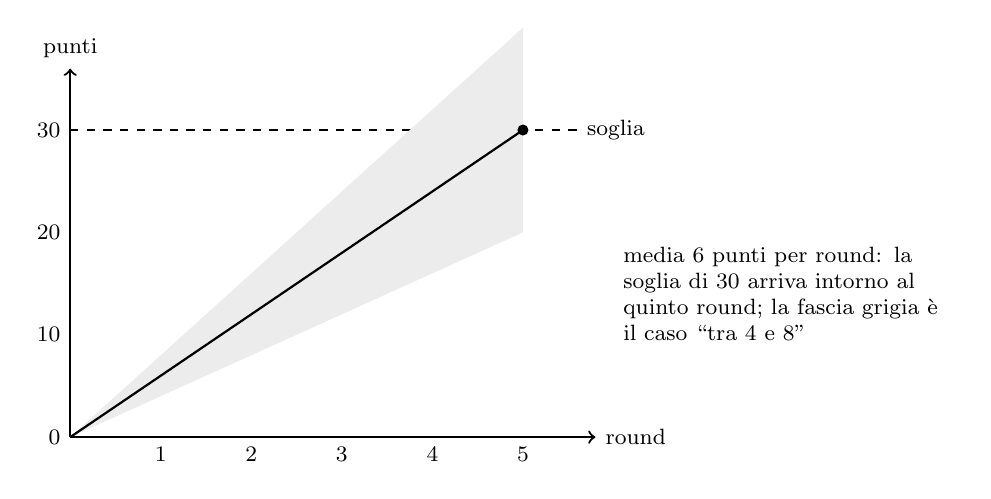
\begin{tikzpicture}[font=\small, x=1.15cm, y=0.13cm]
  \draw[thick, ->] (0,0) -- (5.8,0) node[right, font=\footnotesize] {round};
  \draw[thick, ->] (0,0) -- (0,36) node[above, font=\footnotesize] {punti};
  \foreach \x in {1,...,5} \node[below, font=\footnotesize] at (\x,0) {\x};
  \foreach \y in {0,10,20,30} \node[left, font=\footnotesize] at (0,\y) {\y};
  \draw[dashed] (0,30) -- (5.6,30) node[right, font=\footnotesize] {soglia};
  \fill[gray!15] (0,0) -- (1,4) -- (2,8) -- (3,12) -- (4,16) -- (5,20) -- (5,40) --
    (4,32) -- (3,24) -- (2,16) -- (1,8) -- cycle;
  \draw[thick] (0,0) -- (1,6) -- (2,12) -- (3,18) -- (4,24) -- (5,30);
  \fill (5,30) circle (2pt);
  \node[font=\footnotesize, text width=4.2cm, align=left, anchor=west] at (6.0,14)
    {media 6 punti per round: la soglia di 30 arriva intorno al quinto round; la fascia
    grigia è il caso ``tra 4 e 8''};
\end{tikzpicture}
\caption{Il bilanciamento di durata con una soglia di punti, nell'esempio di Marta su
\emph{Root}: dal numero di round desiderato si ricava quanti punti deve poter fare un
giocatore in un round, e da lì il valore di ogni elemento.}
\label{a14:fig:durata}
\end{figure}

\paragraph{Tagliare i turni iniziali.} Che cosa si può fare per limare la durata? Si possono
\textbf{tagliare i turni iniziali}, che molto spesso presentano \textbf{poche scelte
significative}. Marta non invita a farlo sempre, anzi, ``con molta parsimonia''. Tra addetti
ai lavori si parla di \textbf{bilanciamento di Kramer}\footnote{Così nella trascrizione (``tra
detti e lavori si chiama il bilanciamento di Kramer''). Il riferimento è probabilmente al
designer tedesco Wolfgang Kramer, ma il capitolo non ha trovato una fonte che usi questo nome
per la tecnica.}: si danno \textbf{risorse di partenza} ai giocatori, perché i primi turni non
siano impiegati a raccogliere risorse. Ha delle insidie: rende sicuramente il gioco più
focalizzato e più attento, ma intanto bisogna fare \textbf{un buon bilanciamento delle risorse
iniziali}; e, se le risorse date sono diverse tra i giocatori, bisogna capire se partire con
certe risorse dia \textbf{un vantaggio}. È una cosa da fare \textbf{solo quando è necessaria}.
Alcuni giochi beneficiano di un \textbf{turno iniziale semplice e guidato}, che è anche uno
degli \textbf{strumenti di approcciabilità}: è vero che quei turni si somigliano da una partita
all'altra, ma a volte servono ad agevolare l'ingresso nel gioco. Soprattutto in un gioco
pensato per andare oltre i confini del proprio genere, qualche turno semplice può aiutare le
persone a \textbf{entrare nel flusso}.

\paragraph{Tagliare i turni finali.} Si fa molto spesso negli \textbf{\emph{engine
building}}, i giochi a ``motore economico'', in cui c'è un \emph{feedback} che genera punti
vittoria o risorse, o che comunque avvicina alla condizione di fine partita. Il motore, andando
avanti, diventa sempre più performante; e se da un certo punto cresce in modo
\textbf{lineare o esponenziale}, diventa probabilmente impossibile per gli altri recuperare.
Allora si tagliano i turni finali: ``da questo punto in avanti è chiaro come andrebbe il resto
della partita, non c'è bisogno di giocarla'', per non tediare le altre persone. L'esempio è
\textbf{\emph{Race for the Galaxy}}: la partita finisce quando si esauriscono i
\textbf{gettoni punti} o quando qualcuno ha giocato \textbf{12 carte}. Di solito avviene quando
il motore si è innescato: i turni successivi ripeterebbero quello che si è già visto, perché
le strategie sono ormai impostate.

\paragraph{La durata dentro il turno.} Un'altra parola sulla durata \textbf{intraturno}. Se si
aggiungono tantissime \textbf{microscelte} dentro il turno, la persona si sentirà
\textbf{paralizzata} e spenderà molto tempo. E anche in una situazione normale, con poche
scelte, se per stare dietro a tutte le regole \textbf{vanno via 5 minuti}, quei 5 minuti vanno
\textbf{moltiplicati per il numero di persone e per il numero di round}: la durata di un gioco
cresce molto in fretta. E si stanno ancora omettendo le altre fasi, come quelle di
\textbf{amministrazione} o di \textbf{conteggio dei punti}. Bisogna quindi fare attenzione che
i turni non siano inutilmente lunghi; ma a volte \textbf{un turno lungo può essere molto
soddisfacente}. \emph{Root} dura, a detta di Marta, due ore e mezza, e i suoi turni sono molto
lunghi rispetto ad altri giochi simili; ma senza quei turni e senza quella durata il gioco ne
risentirebbe in termini di esperienza. ``Alla fine conta molto il gioco che stiamo facendo.''

\subsection{La domanda: come si calcola la durata sulla scatola?}

Uno studente chiede: sulle scatole c'è scritto quanto dura un gioco, ma spesso a lui sembra
\textbf{sottodimensionato}. Come viene calcolato? C'è uno standard?

``Lo standard in realtà non c'è'', risponde Marta. Tendenzialmente si dovrebbe indicare
\textbf{la durata media di una partita una volta che si conoscono le regole}. Quindi:
\begin{itemize}
  \item \textbf{non è mai compresa la spiegazione delle regole};
  \item \textbf{non è mai considerata la prima partita}: il valore vale più per chi ha giocato
        tre o quattro volte e conosce il gioco, e non è più al punto di riprendere in mano il
        regolamento.
\end{itemize}
Va da sé che il numero viene \textbf{sbagliato piuttosto spesso}, perché non è facile
stabilirlo. Il metodo migliore, secondo Marta, è prendere \textbf{il tempo medio del gruppo di
\emph{test} che conosce il gioco} e quello di chi fa \textbf{\emph{blind test}}, cioè di persone
alle prime armi, e vedere dove si assesta \textbf{il valore di mezzo}: non tutti giocheranno come
chi ha fatto cento partite, ma neanche ne faranno solo due; l'ideale sarebbe che a un gioco si
facessero \textbf{5--10 partite}. E poi dipende molto dai \textbf{gruppi di gioco}: non c'è un
vincolo su quanto si impiega a fare il proprio turno, e se si è al tavolo con persone che
pensano molto, le durate cresceranno. Si tende comunque a trovare una durata
\textbf{compatibile con il gioco}: un gioco per bambini non può durare due ore, ``ma queste
cose penso le intuite anche voi''.

\paragraph{Approfondimento: corto o lungo.} Schell dedica un intero tipo di bilanciamento
(``corto contro lungo'') alla durata: se il gioco è troppo corto, i giocatori non riescono a
sviluppare ed eseguire strategie significative; se è troppo lungo, si annoiano o lo evitano
per l'impegno di tempo. Le leve principali sono le condizioni di vittoria e di sconfitta. Due
suoi esempi mostrano soluzioni diverse dal taglio di turni: in \emph{Spy Hunter}, per i primi
novanta secondi il giocatore ha auto infinite, perché i principianti non abbiano partite
frustranti di pochi secondi; in \emph{Minotaur}, dopo venti minuti suona una campana e tutti i
sopravvissuti vengono trasportati in una stanza piena di mostri, così la partita finisce in
meno di venticinque minuti e c'è comunque un vincitore, lo stesso principio della zona che si
restringe nei \emph{battle royale}. È convergenza (sezione~\ref{a14:sec:difetti}) imposta per
regola.

% ---------------------------------------------------------------------
\section{Raddoppia o dividi la risorsa}
\label{a14:sec:raddoppia}

Un'altra tecnica ``molto popolare'' è \textbf{raddoppiare o dividere la risorsa}\footnote{Nella
trascrizione ``il raddoppio di vidi la risorsa''.}. A volte è importante capire \textbf{quanto
una risorsa incide sul gioco}, e dove ha senso bilanciarla, se farla crescere o diminuire: non
è sempre semplice capirlo. La tecnica base è: se c'è uno spazio azione dove si ottengono delle
risorse, \textbf{si raddoppia la quantità}, anche se il numero sembra grandissimo,
\textbf{oppure la si divide}. Raddoppiare o dividere è un'\textbf{estremizzazione}, ed
estremizzare una risorsa ne rende subito evidente l'impatto sul gioco: si applica la tecnica e
si vede come reagisce il sistema.

\paragraph{Le dipendenze.} Se la risorsa ha \textbf{tante dipendenze}, il sistema può
``fallire'': la modifica scombina tantissime cose a cascata, e la tecnica diventa praticamente
inutile, perché non restituisce alcun valore certo. Più dipendenze ha, più il rischio è alto.
Per esempio, è \textbf{poco rischioso} applicarla ai \textbf{punti vittoria}: raddoppiare o
dividere i punti di una carta specifica di solito ha poco impatto sul resto delle carte e dei
componenti, perché è \textbf{un valore finale}, con poche dipendenze. Va comunque valutato di
volta in volta.

\paragraph{Quanto deve pesare ogni parte.} Va considerato anche, come questione a sé,
\textbf{quanto valgono le varie parti del gioco}. Se si fa un gioco in cui si costruisce la
propria \textbf{città} sulla propria plancia, e poi ci sono \textbf{obiettivi} e
\textbf{risorse} che danno punti, e il \emph{focus} deve essere la città, allora la città deve
valere \textbf{il 50, 60, anche 70\%} del punteggio totale, riservando il \textbf{10--15\%}
agli altri sistemi che entrano nel conteggio finale. Non è un caso che in
\textbf{\emph{Wingspan}} \textbf{quasi il 50\%} dei punti derivi dalle \textbf{carte uccello} o
dall'uso di determinate abilità, perché sono il \emph{focus} del gioco: difficilmente si fa più
della metà dei punti con le risorse rimaste a fine partita o con le carte obiettivo. È anche una
questione di \textbf{dove mettere il \emph{focus} dell'esperienza}.

\paragraph{Una ricerca progressiva.} La tecnica può essere \textbf{progressiva}: applicando
costantemente il raddoppio o la divisione si arriva a trovare il \textbf{valore medio}. Si
continua a raddoppiare finché la risorsa non diventa \textbf{troppo incisiva}; da lì si torna
a dividere, cioè un po' indietro; e così, stringendo via via il campo, si trova il valore
giusto (figura~\ref{a14:fig:raddoppia}). Anche qui, però, bisogna capire se il valore
``giusto'' è quello che serve a \textbf{veicolare l'intento del \emph{design}}, o se è
semplicemente qualcosa che funziona ma finisce per \textbf{appiattire} il resto delle risorse:
``fare attenzione sempre al solito concetto''.

\begin{figure}[htbp]
\centering
\begin{tikzpicture}[font=\small, x=1.25cm, y=1cm]
  \draw[thick] (0,0) -- (9,0);
  \foreach \x/\l in {0.5/1, 1.5/2, 3.5/4, 7.5/8} {
    \draw (\x,-0.12) -- (\x,0.12);
    \node[below, font=\footnotesize] at (\x,-0.15) {\l};
  }
  \fill[gray!25] (3.5,-0.08) rectangle (7.5,0.08);
  \node[font=\footnotesize] at (5.5,-1.3) {qui sta il valore cercato};
  \draw[-{Stealth[length=2mm]}, thick] (0.5,0.3) to[bend left=40] node[above,
    font=\scriptsize] {$\times 2$} (1.5,0.3);
  \draw[-{Stealth[length=2mm]}, thick] (1.5,0.3) to[bend left=40] node[above,
    font=\scriptsize] {$\times 2$} (3.5,0.3);
  \draw[-{Stealth[length=2mm]}, thick] (3.5,0.3) to[bend left=40] node[above,
    font=\scriptsize] {$\times 2$: troppo!} (7.5,0.3);
  \draw[-{Stealth[length=2mm]}, thick] (7.5,-0.2) to[bend left=40] node[below,
    font=\scriptsize] {a metà strada} (5.5,-0.2);
  \node[font=\footnotesize, text width=4.3cm, align=left, anchor=west] at (9.2,0.2)
    {1: poco incisiva\\ 2, 4: ancora poco\\ 8: troppo incisiva\\ $\Rightarrow$ si torna
    indietro e si stringe tra 4 e 8};
\end{tikzpicture}
\caption{Raddoppia o dividi come ricerca progressiva: si estremizza la risorsa finché il suo
impatto non diventa evidente, poi si torna indietro stringendo l'intervallo. Funziona bene su
valori con poche dipendenze, come i punti vittoria di una carta.}
\label{a14:fig:raddoppia}
\end{figure}

\paragraph{Approfondimento: la regola di Sid Meier.} Schell riporta la stessa tecnica come
``regola del raddoppio e del dimezzamento'': quando si cambia un valore per bilanciare, si
spreca tempo a cambiarlo di poco; conviene raddoppiarlo o dimezzarlo nella direzione in cui
deve andare, e poi, se si è esagerato, provare a metà strada. L'esempio è un razzo che fa 100
punti di danno: se sembrano troppi, non si scende a 90 o 80, ma a 50. La regola è spesso
attribuita a Brian Reynolds, che però, interpellato da Schell, ne dà il merito a \textbf{Sid
Meier}: lo prese da parte, all'inizio degli anni Novanta, mentre lavoravano a
\emph{Colonization}, dopo averlo visto cambiare ripetutamente un valore del 10\%. Il punto,
dice Reynolds, è cambiare qualcosa in modo da \emph{sentire} subito la differenza, invece di
perdersi a chiedersi se si è avuto un effetto, o peggio vederne uno che non c'è, magari per
una serie sfortunata di numeri casuali.

% ---------------------------------------------------------------------
\section{Due problemi, una soluzione}
\label{a14:sec:dueproblemi}

Un'altra tecnica molto usata, soprattutto \textbf{all'inizio dello sviluppo}: \textbf{due
problemi, una soluzione}. Quando si trova un problema, \textbf{non lo si risolve subito}: se ne
cerca \textbf{almeno un altro}, e si applica \textbf{una soluzione a entrambi}, cioè una sola
modifica che li risolva tutti e due. Questo aiuta a \textbf{far convergere il lavoro}, verso
una riduzione del numero di problemi: magari la soluzione ne fa emergere un altro, ma
generalmente \textbf{non ne fa emergere altri due}, e così si progredisce.

È utile all'inizio. Applicata \textbf{verso la fine}, ci si accorge che intanto è \textbf{poco
efficace}, e soprattutto che la soluzione trovata \textbf{impatta molto più forte} su tutti gli
altri sistemi. Il consiglio è di usarla principalmente all'inizio, e di fare attenzione
\textbf{all'impatto di ciascuna leva}: risolvendo due problemi con una nuova soluzione si
modificano leve che a loro volta possono creare problemi. Purtroppo questo si risolve solo in
due modi: con \textbf{l'esperienza}, cioè sapendo più o meno che cosa succede quando si
applicano certe soluzioni, e con i \textbf{\emph{test}}, perché a volte non c'è modo di
risolvere i problemi se non empiricamente.

% ---------------------------------------------------------------------
\section{Gli elementi ricorrenti del bilanciamento}
\label{a14:sec:elementi}

Seguono ``vari elementi'' che ricorrono quando si parla di bilanciamento e di sviluppo, e per
cui Marta non ha trovato ``un modo coerente di metterli'': in questa slide ha cercato di
trasmettere ``quelle cose che si apprendono un po' per esperienza''. La
tabella~\ref{a14:tab:elementi}, alla fine della sezione, li riassume.

\subsection{Le progressioni di punteggio}

Ci sono \textbf{progressioni note} per i punteggi. Una classica è \textbf{1, 3, 6, 10, 15}: tra
un numero e l'altro l'incremento cresce di uno (+2, +3, +4, +5). Serve, per esempio, in una
\textbf{collezione di set}, a rendere la collezione \textbf{sempre più premiante} man mano che
cresce. Una progressione ancora più forte è quella \textbf{quadratica}: con 5 pezzi di una
risorsa si fanno \textbf{25 punti}; cresce molto più rapidamente dell'altra, e quindi si dà
\textbf{ancora più importanza} a quella risorsa. Oppure ci può essere una progressione
\textbf{penalizzante}: dà punti fino a un certo punto, per esempio 1, 3, 6, e poi
\textbf{scende}, 5, 4; dice che quella risorsa la si vuole, \textbf{``ma non troppo''}
(figura~\ref{a14:fig:progressioni}).

Sono elementi che tornano comodi quando si ha una collezione di set e si vuole creare una certa
esperienza in linea con il \emph{design}. Molto spesso la prima cosa che si fa è prendere una
di queste progressioni ``classiche'', applicarla e vedere come reagisce il gioco; ``in rari casi
vengono cambiate''.

\begin{figure}[htbp]
\centering
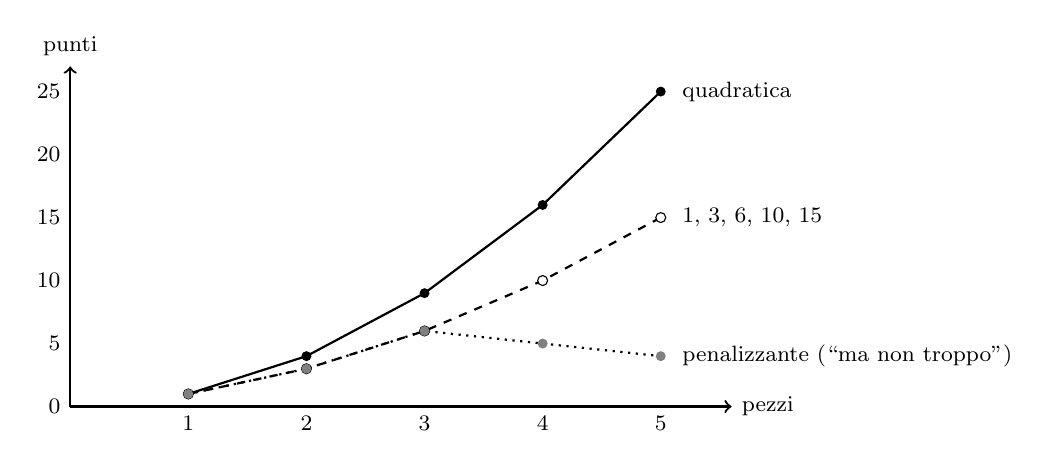
\begin{tikzpicture}[font=\small, x=1.5cm, y=0.16cm]
  \draw[thick, ->] (0,0) -- (5.6,0) node[right, font=\footnotesize] {pezzi};
  \draw[thick, ->] (0,0) -- (0,27) node[above, font=\footnotesize] {punti};
  \foreach \x in {1,...,5} \node[below, font=\footnotesize] at (\x,0) {\x};
  \foreach \y in {0,5,10,15,20,25} \node[left, font=\footnotesize] at (0,\y) {\y};
  % quadratica
  \draw[thick] (1,1) -- (2,4) -- (3,9) -- (4,16) -- (5,25);
  \foreach \x/\y in {1/1,2/4,3/9,4/16,5/25} \fill (\x,\y) circle (1.8pt);
  \node[font=\footnotesize, anchor=west] at (5.1,25) {quadratica};
  % triangolare
  \draw[thick, dashed] (1,1) -- (2,3) -- (3,6) -- (4,10) -- (5,15);
  \foreach \x/\y in {1/1,2/3,3/6,4/10,5/15} \fill[white, draw=black] (\x,\y) circle (1.8pt);
  \node[font=\footnotesize, anchor=west] at (5.1,15) {1, 3, 6, 10, 15};
  % penalizzante
  \draw[thick, dotted] (1,1) -- (2,3) -- (3,6) -- (4,5) -- (5,4);
  \foreach \x/\y in {1/1,2/3,3/6,4/5,5/4} \fill[gray] (\x,\y) circle (1.8pt);
  \node[font=\footnotesize, anchor=west] at (5.1,4) {penalizzante (``ma non troppo'')};
\end{tikzpicture}
\caption{Le tre progressioni di punteggio di cui parla Marta. Più ripida è la curva, più il
gioco spinge a concentrarsi su quella collezione; una curva che scende dopo un massimo dice
che la risorsa serve, ma non in eccesso.}
\label{a14:fig:progressioni}
\end{figure}

\subsection{Mettere in relazione le risorse: moltiplicazioni e set}

\paragraph{La moltiplicazione.} Si possono \textbf{mettere in relazione due risorse}, per
esempio con una \textbf{moltiplicazione}: si ottengono punti pari a \textbf{risorsa A per risorsa
B}. L'intento di sviluppo che questo veicola è che si vogliono \textbf{possibilmente tante A
quante B}, e non tante dell'una e poche dell'altra: per come funziona la moltiplicazione, a
parità di pezzi totali si ottiene di più se i due numeri sono uguali che se uno è molto alto e
l'altro molto basso (con 6 pezzi, $3 \times 3 = 9$, mentre $5 \times 1 = 5$). È una cosa che si
adotta quando si vede che c'è \textbf{troppa concentrazione su una delle due risorse}, magari
perché risulta più premiante: la moltiplicazione le \textbf{ribilancia}, in modo che abbiano lo
stesso interesse.

\paragraph{Il set.} Lo stesso vale per più di due risorse, tre o quattro, quando si vuole che
nel gioco \textbf{siano tutte importanti} e non vengano trascurate: allora si premia
\textbf{il set}. Per ogni set completo, cioè almeno una di ciascuna risorsa, si dà un certo
punteggio.

\paragraph{Punteggio verticale e orizzontale.} Marta non ricorda il termine inglese di
partenza (``mi sfugge il termine'') e li chiama \textbf{punteggio verticale} e
\textbf{punteggio orizzontale}. Il \textbf{verticale} è quello classico: questa risorsa dà
tanto, quest'altra tanto, per quello che ho ottenuto nel gioco. L'\textbf{orizzontale} prende
\textbf{l'altro asse}, e analizza \textbf{quante risorse diverse} ho ottenuto: è il caso, molto
spesso, del calcolo dei set di risorse.

``Anche queste sono tutte cose che trovate standard.'' Ed è anche per questo, come diceva la
volta precedente, che è importante \textbf{giocare tanti giochi}, conoscere tanto, avere
curiosità, esplorare anche giochi \textbf{fuori dalla propria \emph{comfort zone}} e
guardarli con occhio critico: ci si accorge che molte di queste cose sono riusate in
tantissimi giochi.

\subsection{L'esclusività delle risorse}

Si torna all'esempio di \emph{Splendor}: c'è un motivo per cui lì le risorse sono
\textbf{esclusive}, cioè i gettoni sono \textbf{in numero prefissato}. ``Mi sembra che sono
10, ora non sono sicurissima''\footnote{Nel gioco i gettoni gemma sono 7 per colore, più 5
gettoni oro jolly, e se ne usano meno con due o tre giocatori. Il numero esatto non cambia il
ragionamento di Marta.}, per ogni risorsa, e le persone ne possono prendere \textbf{tre a turno}
con la propria azione. Essendo esclusive, il gioco si basa anche sulla \textbf{scarsità}: è una
strategia lecita \textbf{prendere delle risorse per toglierle} agli altri e fare in modo che
non ci siano per le altre persone al tavolo. E l'effetto si propaga: se c'è una carta che
interessa a più giocatori, togliendo la risorsa dal tavolo la carta diventa \textbf{esclusiva a
sua volta}, perché nessun altro la può completare. Poi la cosa si manifesta come un aspetto di
\textbf{\emph{timing}}: diventa importante \textbf{quando} restituire quelle risorse.

\paragraph{Da limite a opportunità.} Marta lo dice perché molto spesso l'esclusività delle
risorse è nata come \textbf{limite}, per via del \textbf{numero di componenti}: essendo un
prodotto fisico, come visto parlando dei limiti della componentistica, è complicato mettere
tante cose in una scatola. Ma, come tutti i limiti, a un certo punto è diventata
un'\textbf{opportunità} di \emph{design} e di sviluppo: quando ci si accorge che c'è
\textbf{poca interazione tra i giocatori}, introdurre l'esclusività delle risorse a volte fa
esattamente quello che serve per \textbf{generare interazione}. Lo stesso vale per gli
\textbf{incentivi}, sia nel restituire queste risorse sia nel prenderle, nel caso la risorsa
sia esclusiva ma i giocatori non la prendano in considerazione.

\subsection{La crescita tra i round}

Un altro aspetto importante è la \textbf{crescita tra round}. In molti giochi è importante che
tra un round e l'altro \textbf{ci sia una differenza}: se in tutti i round si ha accesso alle
stesse identiche risorse, la stessa situazione sulla plancia, le stesse possibilità, il gioco
risulta \textbf{statico}. La crescita fa percepire \textbf{la progressione} a chi gioca. A volte
viene tralasciata, ma si può fare in modo abbastanza semplice: se c'è una \textbf{rendita}, la
rendita cresce; oppure, man mano che si piazzano cose sul tabellone, si \textbf{sbloccano} cose
sulla propria plancia che danno più possibilità andando avanti. È un elemento che nello
sviluppo viene esaminato molto spesso, perché magari il gioco funziona, ma ha \textbf{una
crescita piatta}, e bisogna lavorare per farla aumentare.

\subsection{Il controllo dell'alea e del caos}

Altro elemento frequente: il \textbf{controllo dell'alea o del caos}. Il gioco può presentare
sia alea sia caos, ma in modo \textbf{estremizzato}, e allora bisogna trovare strumenti per
regolarli. L'esempio più classico: \textbf{lancio un dado e spendo una risorsa per fare il
\emph{re-roll}}. Molti giochi con questa meccanica non avevano di base il \emph{re-roll}: è
stato aggiunto \textbf{in fase di sviluppo}, perché si è visto che il lancio di dado senza
possibilità di rilancio è un'esperienza \textbf{frustrante} per la maggior parte di chi gioca.
C'è poi l'esempio pratico di \textbf{\emph{Magical Athlete}}, che ha ``abbattuto un po' questa
concezione'': oggi ci sono giochi che accettano ``un po' più di buon grado'' anche il lancio
del dado senza controllo. Ma in fase di sviluppo questo resta uno degli elementi su cui si va a
incidere. Un altro esempio: tessere pescate \textbf{da un sacchetto}, con la possibilità di
\textbf{pescarne più di una}, o di \textbf{rimettere} quella pescata e pescarne un'altra.

\subsection{Le probabilità}

È utile avere \textbf{una base di probabilità}. L'esempio più classico è il dado, e sapere come
usare i dadi in un gioco ``può fare la differenza''.

\paragraph{Lineare.} Un dado da 1 a 6 ha una probabilità cosiddetta \textbf{lineare}
(uniforme): ogni faccia ha la stessa probabilità di uscire.

\paragraph{A campana.} Con \textbf{due dadi} la probabilità segue una \textbf{curva a campana}:
il risultato medio è più probabile dei risultati agli estremi. ``Penso che questo lo sappiate'':
con due dadi è molto più probabile fare \textbf{7} che fare 2 o 12. È una particolarità che può
\textbf{informare le decisioni}. Si immagini un \textbf{gioco di percorso} in cui si lancia un
solo dado: si dà la stessa probabilità a tutte le facce, e mediamente ci si muove di
\textbf{3,5}, il valore medio di un dado. Con due dadi, invece, uscirà più spesso il 7: è un
sistema ``più morbido'', perché i risultati estremi sono più rari. Con un dado solo, il 6 può
uscire tanto quanto il 3 o il 4, e solo su molti lanci la media si riporta a 3,5. Questo aiuta
a capire che cosa serve in funzione del gioco (figura~\ref{a14:fig:dadi}).

\paragraph{Calante.} La probabilità può anche essere \textbf{calante}. Si immagini di poter
scegliere quante risorse ottenere, \textbf{da una a cinque}, ma per ogni risorsa voluta bisogna
\textbf{lanciare una moneta}. Se se ne prende una, si lancia una moneta: con testa la si tiene,
con croce no. Se se ne vogliono cinque, si lanciano cinque monete, ma \textbf{basta una sola
croce per non tenerne nessuna}. La probabilità \textbf{cala} al crescere delle risorse che si
vogliono ottenere. Si usa anche questo: per esempio, in un gioco di percorso, ``posso muovermi
di quanto mi pare, ma poi lancio il dado'', e se il risultato è inferiore allo spostamento
dichiarato devo tornare indietro, o non mi muovo affatto.

Sono piccoli meccanismi che influenzano e guidano le scelte, e che aiutano a regolare lo
sviluppo: magari in fase di \emph{design} si è detto ``mi interessa che sia un gioco di
percorso, mi basta lanciare un dado da 6 e andare dove vado''; ma in sviluppo si vuole che la
decisione sia \textbf{più controllata}, e si possono inserire strutture come il
\textbf{cambiare la probabilità} di quel meccanismo.

\begin{figure}[htbp]
\centering
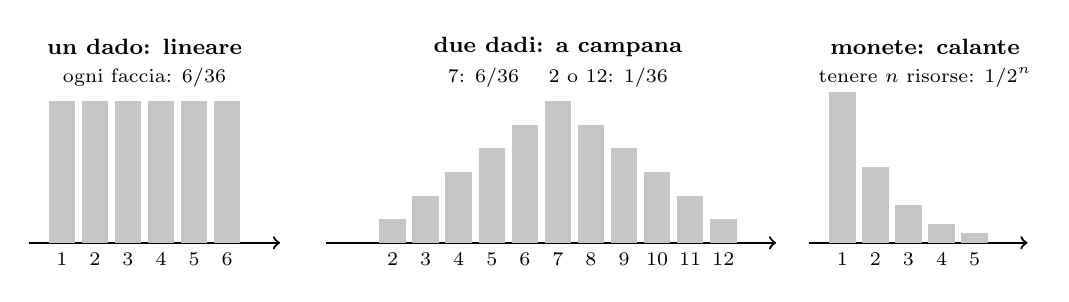
\begin{tikzpicture}[font=\small, x=0.42cm, y=0.30cm]
  % un dado
  \node[font=\footnotesize\bfseries] at (3.5,8.3) {un dado: lineare};
  \draw[thick, ->] (0,0) -- (7.6,0);
  \foreach \v in {1,...,6} {
    \fill[gray!45] (\v-0.4,0) rectangle (\v+0.4,6);
    \node[below, font=\scriptsize] at (\v,0) {\v};
  }
  \node[font=\scriptsize] at (3.5,7.0) {ogni faccia: 6/36};
  % due dadi
  \begin{scope}[shift={(9,0)}]
    \node[font=\footnotesize\bfseries] at (7,8.3) {due dadi: a campana};
    \draw[thick, ->] (0,0) -- (13.6,0);
    \foreach \v/\h in {2/1,3/2,4/3,5/4,6/5,7/6,8/5,9/4,10/3,11/2,12/1} {
      \fill[gray!45] (\v-0.4,0) rectangle (\v+0.4,\h);
      \node[below, font=\scriptsize] at (\v,0) {\v};
    }
    \node[font=\scriptsize] at (7,7.0) {7: 6/36 \quad 2 o 12: 1/36};
  \end{scope}
  % monete
  \begin{scope}[shift={(23.6,0)}]
    \node[font=\footnotesize\bfseries, align=center] at (3.5,8.3) {monete: calante};
    \draw[thick, ->] (0,0) -- (6.6,0);
    \foreach \v/\h in {1/6.4,2/3.2,3/1.6,4/0.8,5/0.4} {
      \fill[gray!45] (\v-0.4,0) rectangle (\v+0.4,\h);
      \node[below, font=\scriptsize] at (\v,0) {\v};
    }
    \node[font=\scriptsize, align=center] at (3.5,7.0) {tenere $n$ risorse: $1/2^n$};
  \end{scope}
\end{tikzpicture}
\caption{Le tre forme di probabilità dell'esempio di Marta: il dado singolo (ogni faccia
ugualmente probabile, media 3,5), due dadi (il 7 è sei volte più probabile del 2 o del 12) e la
probabilità calante delle monete (per tenere $n$ risorse servono $n$ teste di fila: 50\%,
25\%, 12,5\%\ldots). Le barre sono in scala all'interno di ciascun grafico.}
\label{a14:fig:dadi}
\end{figure}

\begin{table}[htbp]
\centering
\small
\begin{tabular}{@{}p{3.2cm}p{5.2cm}p{5.0cm}@{}}
\toprule
\textbf{Tecnica o elemento} & \textbf{Che cosa fa} & \textbf{Attenzione a} \\
\midrule
Budget di complessità & ciò che si toglie libera complessità, da eliminare o reinvestire
  nel \emph{focus} & nel dubbio, meglio accessibile \\
\addlinespace
Alto e basso rischio & crea una scelta sensibile con due macro-strategie comunicanti & la
  ricompensa deve valere il rischio \\
\addlinespace
Ancoraggio & tutto è rapportato a un valore ancora (\emph{Stone Age}: un puntino = un punto)
  & risorse interdipendenti, turni extra, \emph{draft} \\
\addlinespace
Durata & round o soglie fissate $\Rightarrow$ punti per round $\Rightarrow$ valore dei
  pezzi; tagliare turni iniziali o finali & la durata intraturno si moltiplica per persone
  e round \\
\addlinespace
Raddoppia o dividi & estremizza per vedere l'impatto, poi stringe & le dipendenze; il
  valore ``giusto'' può appiattire \\
\addlinespace
Due problemi, una soluzione & fa convergere il lavoro & solo all'inizio dello sviluppo \\
\addlinespace
Progressioni & 1-3-6-10-15, quadratica, penalizzante & che cosa si vuole premiare \\
\addlinespace
$A \times B$ e set & spingono a bilanciare le risorse tra loro & punteggio verticale contro
  orizzontale \\
\addlinespace
Esclusività & scarsità, interazione, \emph{timing} & nata come limite di componenti \\
\addlinespace
Crescita tra round & progressione percepita (rendite, sblocchi) & la crescita piatta \\
\addlinespace
Controllo dell'alea & \emph{re-roll}, più pescate, rimettere nel sacchetto & non sempre serve
  (\emph{Magical Athlete}) \\
\addlinespace
Probabilità & lineare, a campana, calante & scegliere la forma che serve all'esperienza \\
\bottomrule
\end{tabular}
\caption{Gli strumenti di bilanciamento presentati nella lezione, nell'ordine in cui li
presenta Marta.}
\label{a14:tab:elementi}
\end{table}

\paragraph{Approfondimento: la probabilità per chi progetta.} Schell dedica un capitolo alla
probabilità con dieci ``regole'', e una delle sue osservazioni conferma il consiglio di Marta
di testare invece di calcolare: il \emph{metodo Monte Carlo}, cioè ripetere la prova molte volte
e contare i risultati, ``a volte dà risultati più utili della probabilità teorica, perché è una
misura della cosa reale''. La sua ultima regola, scherzosa, è la più pratica: quando un calcolo
si fa difficile, cercare qualcuno che si consideri ``un mago della matematica'', che ne sarà
entusiasta. Brathwaite e Schreiber, in \emph{Challenges for Game Designers}, dedicano invece un
intero capitolo all'equilibrio tra caso e abilità, il tema del controllo dell'alea.

% ---------------------------------------------------------------------
\section{Smussare la stella}
\label{a14:sec:stella}

``Vediamo, ok. Forse devo correre un po', allora.'' \textbf{Non è detto che chi crea il gioco
abbia chiaro il \emph{design}.} Per spiegarlo Marta usa un modo di dire: un gioco è
\textbf{una stella}, e lo sviluppo \textbf{smussa gli angoli}, perché le punte non blocchino
l'ingresso in un ipotetico buco (``non so come dirlo meglio''). Le punte rappresentano le
\textbf{qualità e le particolarità del \emph{design}}. Come detto la volta prima, il
\emph{design} è anche \textbf{personale} e dovrebbe sfuggire un po' alle logiche di mercato; e
così anche lo sviluppo. Oggi tenere alcune punte è diventato più importante che in passato;
tuttavia si smussa, perché \textbf{più punte ha la stella, meno è digeribile per un pubblico
ampio}: le persone hanno bisogno di un po' di \textbf{familiarità} e di un po' di
\textbf{novità}, non accettano una cosa totalmente innovativa, ma neanche ne vogliono una
estremamente familiare. È un gioco di \textbf{trovare il punto giusto}.

\paragraph{Chi ha creato il gioco può non vedere l'intento.} In questo, a volte, anche chi ha
creato il gioco ha poco chiaro l'intento del \emph{design}, nonostante il gioco lo manifesti:
viene fuori giocandolo. Lo sviluppo deve però evitare di \textbf{finire sui \emph{bias}
personali}: se si ha un genere preferito, bisogna fare attenzione a non mettere la propria
preferenza in tutti i giochi. Se si fa un gioco per bambini, è inutile metterci le dinamiche di
un \textbf{motore economico}: ``non funziona'', o quanto meno sarà molto complicato far capire a
un bambino come funziona economicamente un motore di gioco. ``So che sembra una banalità'', ma è
una tendenza in cui si cade con estrema facilità, anche in casi che sembrano estremi.

\paragraph{Il GCD come bussola.} Il \textbf{\emph{Game Concept Document}} dà il \emph{focus} per
restare sul progetto: averlo sempre a portata di mano aiuta a ricordare che cosa si sta
facendo, come lo si sta facendo, e \textbf{che cosa si può davvero smussare} senza intaccare
uno dei \textbf{pilastri}, cosa che comprometterebbe davvero il \emph{design}. Resta il fatto che
\textbf{se una cosa non è fondamentale all'esperienza, può essere tolta}.

\paragraph{Ma attenzione a che cosa è ``fondamentale''.} La valutazione personale porta sempre
il rischio di sbagliarsi. Una cosa che \textbf{sembra} non fondamentale, come i \textbf{testi di
ambientazione} (\emph{flavor text}) su alcune carte, solo perché non entrano in gioco in modo
meccanico, a volte viene considerata non incisiva. Ma se \textbf{\emph{Wingspan}} non avesse i
testini che raccontano i comportamenti degli uccelli e tutto il resto, probabilmente non avrebbe
la stessa potenza, la stessa capacità di fare leva su tantissime persone che ha avuto nella
pratica. Alcune cose non sembrano fondamentali, ``ma fanno la differenza''.

\paragraph{Approfondimento: l'eleganza e il dettaglio.} Schell elenca tra i dodici tipi di
bilanciamento anche ``semplice contro complesso'' e ``dettaglio contro immaginazione'', e
propone una \emph{lente dell'eleganza}: un sistema elegante fa molto con pochi elementi. Ma per
lui l'eleganza non è il taglio indiscriminato: i dettagli che \emph{nutrono} l'immaginazione,
e che l'immaginazione può riusare più e più volte, vanno tenuti. I testi di \emph{Wingspan} sono
esattamente questo tipo di dettaglio.

% ---------------------------------------------------------------------
\section{I ``difetti'' dei giochi da tavolo}
\label{a14:sec:difetti}

``Ok, vediamo alcuni dei difetti cosiddetti dei giochi da tavolo.'' Le virgolette sono volute:
molte di queste cose vengono elencate come difetti, \textbf{ma non lo sono}. Lo sono se sono
\textbf{una dinamica che va contro l'esperienza attesa}: ``tendenzialmente sì, se va contro
l'esperienza attesa, di fatto lo possiamo chiamare difetto''. Ma \textbf{non esistono meccaniche
che siano difetti a priori}: vanno viste in funzione del gioco. Molto spesso le persone
confondono le meccaniche che generano \textbf{stati d'animo negativi} (la
\textbf{frustrazione}, a volte la \textbf{noia}) con difetti del gioco. Non è sempre così.
\textbf{Attenzione ai \emph{feedback}}, quindi: molto spesso vi elencheranno queste cose come
difetti, e non è detto che lo siano. Una slide lo riassume: bisogna distinguere
\textbf{l'intento del \emph{design}} dalle \textbf{dinamiche incontrollate}. Il ``difetto'' era
un intento del \emph{design}, oppure è lì perché è un \textbf{aspetto vestigiale del genere}, e
genera dinamiche che neanche il designer sa controllare? La tabella~\ref{a14:tab:difetti} li
riassume.

\paragraph{L'eliminazione dei giocatori: \emph{Bang!}.} La \textbf{\emph{player elimination}}
viene prima perché probabilmente la conoscono tutti, per via di \textbf{\emph{Bang!}}. Tantissime
persone si lamentano di \emph{Bang!} perché c'è l'eliminazione dei giocatori, ma poche si
rendono conto che \textbf{\emph{Bang!} senza eliminazione non funzionerebbe}: sarebbe un gioco
poco efficace. L'eliminazione garantisce che \textbf{tutta la partita sia giocata in tensione};
che non si possano \textbf{scaricare le risorse} liberamente senza pensarci, perché poi si
giocherebbe tutta la partita senza risorse; e fa tutta la differenza sulle
\textbf{ritorsioni}: in certi casi ``posso permettermi di finire le risorse perché so che non
subirò ritorsioni'', cosa che senza eliminazione non sarebbe possibile. La narrativa sottesa di
\emph{Bang!}, e il motivo per cui continua a piacere a tantissime persone, è legata anche
all'eliminazione: è un gioco sul \textbf{Far West}, in un certo senso spietato, che vuole
trasmettere una narrativa con \textbf{\emph{high stakes}}, una posta in gioco
altissima\footnote{Marta dice ``delle \emph{high stakes}, delle alte\ldots{} non mi torna il
termine italiano, perdonatemi''.}. Ci sono però giochi in cui l'eliminazione è \textbf{poco
giustificata}: in un gioco in cui si coopera per salvare il pianeta, ha poco senso eliminare
un giocatore a caso, ``adesso faccio per dire; poi magari trovate la chiave di lettura per cui
ha senso''.

\paragraph{\emph{Runaway leader} e \emph{bash the leader}: \emph{Root}.} Anche queste sono
spesso viste come negative. Il \textbf{\emph{runaway leader}} è quando un giocatore prende un
distacco tale che diventa difficile recuperarlo. La dinamica contrapposta è il \textbf{\emph{bash
the leader}}\footnote{Nella trascrizione ``Base the Leader'' e ``best dei leader''.}: le persone
individuano chi potrebbe ``correre via'' e vincere, e lo \textbf{bastonano}, letteralmente;
tutti se la prendono con la stessa persona, quella in testa. Entrambe possono essere utili in
giochi che rappresentano \textbf{dinamiche di potere}. \emph{Root}, che rappresenta proprio le
dinamiche di potere tra fazioni diverse, ha fatto del \emph{bash the leader} una delle sue
caratteristiche peculiari: il designer l'ha voluta mettere dentro con l'obiettivo di far
ruotare il gioco attorno a questa cosa. Non è una dinamica non voluta: è
\textbf{desiderata}, e il gioco dà gli strumenti sia per metterla in pratica sia per evitare che
diventi incontrastabile.

\paragraph{I \emph{feedback loop}.} Sono quando le risorse o i meccanismi di gioco
\textbf{informano la decisione successiva}. Un \emph{feedback loop} \textbf{positivo}: spendo
risorse e ottengo punti vittoria, e magari un'altra risorsa, che posso usare per ottenere altri
punti e altre risorse: ``capite che cresce all'infinito''. Un \emph{feedback loop}
\textbf{negativo}: eseguire qualcosa non dà qualcosa che rinforza il ciclo, e quindi rifarlo non
è premiante, e questo smorza le fasi successive. Sono dinamiche da tenere d'occhio, perché
possono compromettere l'intento.

\paragraph{Il \emph{kingmaking}.} ``Il \emph{kingmaking} è un'altra\ldots{} vabbè'': Marta non si
dilunga, ``se avete qualche curiosità''\footnote{Il \emph{kingmaking} è la situazione in cui
un giocatore che non può più vincere decide, con le sue mosse, chi tra gli altri vincerà.}.

\paragraph{Divergenza e convergenza.} Le trova ``sempre interessanti''. Molto spesso i giochi
\textbf{non convergono}, cioè non arrivano a una fine: il \emph{design} magari è bello, ma chi
l'ha creato \textbf{non ha pensato a come finisce}, e il gioco può \textbf{stallare}, non
concludersi mai. Bisogna sapere come farlo convergere, e ci sono meccanismi per farlo. Se la
fine del gioco è legata alla \textbf{fine del mazzo}, in un gioco in cui le carte vengono
\textbf{rimesse nel mazzo}, c'è \textbf{divergenza}: il gioco potrebbe non finire mai, perché il
mazzo non finisce mai. Se invece le carte pescate \textbf{non vengono reinserite} in nessun modo
e ogni turno se ne devono pescare \textbf{due}, si sa che \textbf{entro $n/2$ turni la partita
sarà finita}, con $n$ carte nel mazzo (figura~\ref{a14:fig:convergenza}). ``Vedete, questi
valori un po' così, perché è un po' diverso il valore vero; tuttavia fate finta che ora vada
bene''\footnote{La precisazione di Marta è giusta: se a pescare sono più giocatori, o se ci sono
altri modi di consumare il mazzo, il conto cambia. Il principio, cioè che una risorsa che si
consuma senza tornare indietro garantisce la fine, resta.}.

\begin{figure}[htbp]
\centering
\begin{tikzpicture}[
  font=\small,
  a14b/.style={draw, thick, rounded corners=3pt, text width=2.0cm, align=center,
               minimum height=0.9cm, fill=white},
  a14arr/.style={-{Stealth[length=2.5mm]}, thick}
]
  \node[font=\footnotesize\bfseries] at (2.0,1.6) {divergente};
  \node[a14b] (m1) at (0,0) {mazzo};
  \node[a14b] (g1) at (4,0) {gioco};
  \draw[a14arr] (m1.north east) to[bend left=25] node[above, font=\footnotesize] {pesca}
    (g1.north west);
  \draw[a14arr] (g1.south west) to[bend left=25] node[below, font=\footnotesize]
    {rimetti nel mazzo} (m1.south east);
  \node[font=\footnotesize, text width=4.6cm, align=center] at (2.0,-1.75) {il mazzo non
    finisce mai: la partita può stallare};
  \node[font=\footnotesize\bfseries] at (9.0,1.6) {convergente};
  \node[a14b] (m2) at (7,0) {mazzo da $n$ carte};
  \node[a14b] (g2) at (11,0) {scarti};
  \draw[a14arr] (m2) -- node[above, font=\footnotesize] {2 a turno} (g2);
  \node[font=\footnotesize, text width=4.6cm, align=center] at (9.0,-1.75) {niente torna
    indietro: entro circa $n/2$ turni la partita finisce};
\end{tikzpicture}
\caption{Divergenza e convergenza nell'esempio di Marta: legare la fine della partita alla fine
di un mazzo funziona solo se il mazzo si consuma davvero.}
\label{a14:fig:convergenza}
\end{figure}

\paragraph{L'ordine di turno.} Infine, attenzione all'\textbf{ordine di turno}: come sono
disposti i giocatori può \textbf{influenzare la partita di chi segue}, e il \textbf{primo
giocatore} potrebbe avere dei vantaggi. Anche \textbf{come sono distribuite le risorse
iniziali} tra i giocatori va guardato con attenzione. L'esempio classico è fare una serie di
\emph{test} attenti proprio a questo: se faccio iniziare sempre la stessa persona e questa
vince sistematicamente, da qualche parte c'è un problema. Questo è uno di quei casi che
``raramente può non essere un difetto: tendenzialmente lo è''. Ma anche qui c'è un'eccezione:
in un gioco che vuole mostrare \textbf{meccanismi di potere diversi}, il primo giocatore può
essere avvantaggiato di proposito. Marta pensa a \textbf{\emph{Il Grande Dalmuti}}, in cui il
Grande Dalmuti, che comincia a giocare, è avvantaggiato: ma quello è un gioco che vuole proprio
far percepire \textbf{la differenza di potere} tra i giocatori al tavolo\footnote{\emph{Il Grande
Dalmuti} è anch'esso di Richard Garfield (1995).}.

\begin{table}[htbp]
\centering
\small
\begin{tabular}{@{}p{3.0cm}p{4.8cm}p{5.6cm}@{}}
\toprule
\textbf{``Difetto''} & \textbf{Che cos'è} & \textbf{Quando è voluto (esempio di Marta)} \\
\midrule
\emph{Player elimination} & un giocatore esce dalla partita & \emph{Bang!}: tensione, niente
  risorse sprecate, ritorsioni, narrativa del Far West \\
\addlinespace
\emph{Runaway leader} & un distacco irrecuperabile & in giochi sulle dinamiche di potere \\
\addlinespace
\emph{Bash the leader} & tutti contro chi è in testa & \emph{Root}: il gioco ruota attorno a
  questo, e dà strumenti per farlo e per evitarlo \\
\addlinespace
\emph{Feedback loop} & positivo: cresce all'infinito; negativo: rifare non premia & da tenere
  d'occhio rispetto all'intento \\
\addlinespace
\emph{Kingmaking} & chi non può vincere decide chi vince & (non approfondito) \\
\addlinespace
Divergenza & il gioco non converge, stalla & mai: va fatto convergere \\
\addlinespace
Ordine di turno & chi inizia vince sistematicamente & raramente: \emph{Il Grande Dalmuti}, che
  vuole far sentire la differenza di potere \\
\bottomrule
\end{tabular}
\caption{I ``difetti'' dei giochi da tavolo: dinamiche che diventano difetti solo se vanno
contro l'esperienza attesa. La domanda è sempre se siano intento del \emph{design} o dinamiche
incontrollate, magari vestigia del genere.}
\label{a14:tab:difetti}
\end{table}

\paragraph{Approfondimento: \emph{feedback} positivo e durata.} Il caso del \emph{runaway
leader} è lo stesso problema dei turni finali degli \emph{engine building}: un ciclo di
\emph{feedback} positivo che rende la partita decisa prima della fine. Le soluzioni viste in
lezione sono tre e si possono combinare: chiudere la partita quando il motore si è innescato
(\emph{Race for the Galaxy}), dare agli altri giocatori strumenti per frenare chi è in testa
(\emph{Root}), o introdurre cicli negativi che smorzino il vantaggio. Schell nota, a proposito
di \emph{Monopoly}, quanto la durata dipenda da queste dinamiche: giocato con le regole
ufficiali dura circa novanta minuti, ma molti gruppi aggiungono \emph{house rules} (premi in
denaro, meno obblighi di acquisto) che rallentano la convergenza e lo portano a tre ore o più.

% ---------------------------------------------------------------------
\section{La domanda sulle sinergie: bilanciare per tentativi}
\label{a14:sec:sinergie}

Le slide successive contengono una serie di esempi tratti da giochi commerciali; ma
``visto che ci avviamo a conclusione'', Marta preferisce dare la precedenza alle domande.

Ne arriva una da uno studente che, si scusa, sta \textbf{guidando} (``scusate, sono in
macchina''). Gli strumenti visti gli sono sembrati molto utili, ma c'è una cosa che farebbe
ancora fatica a fare. Si immagini un \textbf{\emph{engine building}} in cui le singole carte
hanno un certo valore, ma \textbf{il loro valore combinato è più alto della somma dei valori
singoli}: tutti i casi in cui una strategia vale più delle componenti che la formano.
\textbf{Come si bilanciano?}

``Mi sembra un caso molto specifico'', risponde Marta: ``chiaramente non ho una bacchetta
magica''. Andrebbe visto nel dettaglio, capendo le dipendenze. ``Così a naso'': se le carte da
sole valgono poco e insieme valgono di più, si sta \textbf{premiando il set di quelle carte}.
Bisogna capire \textbf{quante sinergie} hanno queste carte, \textbf{con quante carte} si
sinergizzano, quali sono i \textbf{percorsi di vittoria} che ci si è figurati nel gioco, e
analizzarle. Poi una risposta più pratica:
\begin{itemize}
  \item \textbf{partire da un bilanciamento per tentativi}: mettere dei numeri, anche un po' a
        caso, ``e vai un po' a sentimento'', e vedere come reagisce il gioco. Se i valori sono
        sballati, c'è qualcosa che non va alla radice: provare altri valori;
  \item \textbf{partire da qualcosa di conosciuto}: prendere giochi simili, guardare i valori
        che usano e provare a riportarli nel proprio;
  \item se si trovano valori che fanno girare l'esperienza ma si teme che non sia bilanciata,
        usare il \textbf{raddoppia o dividi}: che succede se \textbf{raddoppio il valore} che
        danno le carte quando sinergizzano? È l'esperienza che voglio? Voglio premiare la
        sinergia? Allora ha senso che diano un valore molto maggiore delle carte singole;
  \item se invece si vogliono tenere le due cose più in equilibrio, ci si chiede se si può
        \textbf{raddoppiare il valore delle carte singole}, e si guarda come reagiscono. Ma
        ``viene da sé'' che, se i valori singoli superano il valore sinergico, la domanda
        diventa: \textbf{perché dovrei farle sinergizzare?}
\end{itemize}
Mancano tante parti del gioco per rispondere fino in fondo, ma il consiglio è di procedere
\textbf{per tentativi}: ``un modo di bilanciare si dice proprio bilanciamento per tentativi, ed
è uno dei metodi più usati''. Lo studente ringrazia: gli piace l'idea di considerare
\textbf{una strategia composta da più carte come un set}, ``è un po' di mentalità che aiuta''.

\paragraph{Il valore sballato.} Marta aggiunge: il bilanciamento, ma tutto lo sviluppo, ``è una
cosa che viene facendo''. Mettendo le mani in pasta l'esperienza conta tanto e diventa più
chiaro quali valori usare; ma non va necessariamente fatto bene la prima volta. ``L'altro ieri''
stava bilanciando un gioco a cui lavora e ha messo \textbf{un valore praticamente sballato}; se
n'è accorta tardi, e il \emph{test} è andato così. Ha cercato di tenere a mente che c'era
questa \textbf{``variabile un po' impazzita''} e si è chiesta: che cosa mi può dire, adesso? Come
mi può informare? Se \textbf{tutti la prendono}, è una carta molto ``golosa'', e bisogna farci
attenzione anche quando la si riporta al valore normale; e se è bastato quel cambio per
attirare l'attenzione su di lei, \textbf{forse il valore di partenza non era così male}, e
c'era qualche altro motivo per cui non veniva presa. Anche un errore, insomma, porta a dei
ragionamenti.

\paragraph{Approfondimento: allenare l'intuito.} Schell suggerisce un esercizio che rende meno
casuale il ``bilanciamento per tentativi'': \emph{indovinare con precisione}. Se un proiettile
si muove a 10 unità al secondo e sembra lento, non si prova ``un po' di più'', ma si cerca il
numero esatto che l'intuito suggerisce (13,8?), lo si prova, e si confronta il risultato con la
previsione. Ogni tentativo diventa un dato per l'intuito, come fa Marta con la sua variabile
impazzita: non un fallimento, ma un'informazione.

% ---------------------------------------------------------------------
\section{Gli esempi: scelte di sviluppo in giochi pubblicati}
\label{a14:sec:esempi}

Non ci sono altre domande, e Marta usa ``questi ultimi dieci minuti'' per mostrare un paio
degli esempi, ``giusto per dirvi delle cose che sono emerse a livello di sviluppo; spero di
incuriosirvi''.

\subsection{\emph{Carcassonne} a tre tessere}

\slidefig{img/AGD/agd14-carcassonne}{Carcassonne.}{slide \emph{Tecniche di sviluppo}}{fig:agd14-carcassonne}


Il primo ``non è un vero e proprio sviluppo''. In \textbf{\emph{Carcassonne}} si piazzano
tessere su un campo comune e si piazzano i propri \emph{meeple}\footnote{Nella trascrizione
``mee-paul'' e ``people''.} sugli elementi della tessera appena piazzata; quando un elemento
viene \textbf{chiuso} dalle altre tessere, il \emph{meeple} viene ripreso e si fanno punti,
generalmente in base alla dimensione della strada o della città. Normalmente si
\textbf{pesca una tessera}, la si piazza e si decide se mettere o no il \emph{meeple}.

C'è una \textbf{variante molto popolare} che consiste nel giocare \textbf{con tre tessere in
mano}: se ne sceglie una da piazzare e poi si ripesca. Spesso viene presentata come
un'affermazione: la versione a tre tessere \textbf{è migliore}, perché c'è \textbf{meno
incidenza della fortuna}: ho sempre una scelta tra tre, invece di pescare a caso e piazzare.
Le preferenze individuali ``non si commentano'', perché magari alle persone piace così. Ma molte
persone non sanno che questo cambiamento genera \textbf{importanti squilibri}.

\paragraph{I \emph{meeple} perdono il loro peso.} Con tre tessere posso \textbf{riservarmi} le
tessere che servono a chiudere una strada o una città per più avanti, e quindi gestire molto
più facilmente \textbf{quando riprendere i \emph{meeple}}. Nel gioco i \emph{meeple} sono
\textbf{sette}, una risorsa limitata: quando li ho piazzati tutti, se piazzo una tessera e non ho
\emph{meeple}, non posso prenderne gli elementi e i punti. È una \textbf{dinamica voluta dal
gioco}. Se invece ho sempre questo \textbf{``cuscinetto''} in mano, questa dimensione sparisce
quasi completamente, perché avrò sempre dei \emph{meeple} disponibili. E allora la domanda è:
``perché limitarli, a quel punto?''. In questo tipo di partita si perde molto il senso di
questo aspetto del gioco.

\paragraph{I monasteri diventano piatti.} Un'altra dinamica spesso fraintesa è quella dei
\textbf{monasteri}. Nel gioco ce ne sono \textbf{sei}: un monastero va \textbf{completamente
circondato}, ogni tessera che lo circonda vale un punto, e quando è completamente circondato si
riprende il proprio \emph{meeple}. Giocando con una sola tessera sembra che la fortuna incida
molto: ``o lo pesco o non lo pesco''. Ma poter scegliere \textbf{quando} piazzarlo cambia
profondamente la dinamica:
\begin{itemize}
  \item \textbf{con una tessera}, si è costretti a giocare \textbf{d'anticipo} e sulle
        probabilità, a capire quando ha senso rischiare, a \textbf{costruirsi il territorio}
        perché il monastero possa svilupparsi;
  \item \textbf{con tre tessere}, il monastero lo si tiene in mano finché non si trova il
        momento opportuno, e tendenzialmente si \textbf{massimizzano i punti}. Se tutti sono
        allo stesso livello di abilità, la massimizzazione si traduce in \textbf{un'esperienza
        piatta}, in cui i monasteri valgono tutti più o meno lo stesso punteggio.
\end{itemize}
Con una tessera c'è incidenza della fortuna nella pesca, ``che, ripeto, c'è anche nell'altra
versione''. Ma \textbf{aver preparato il terreno} al monastero e piazzarlo nel momento giusto fa
tutta la differenza tra \textbf{una giocata di abilità} e una in cui una persona non si è
costruita l'opportunità, o non nel momento giusto. ``C'è un motivo, ed è un motivo anche molto
intelligente, per cui si gioca con una sola tessera e non con tre a \emph{Carcassonne}'',
tranne, appunto, se piace e si vuole fare la \emph{house rule}.

\subsection{\emph{Bonsai}: togliere i punti al legno}

\slidefig{img/AGD/agd14-bonsai}{Bonsai e Bonsai Wabi Sabi.}{slide \emph{Tecniche di sviluppo}}{fig:agd14-bonsai}


Il secondo esempio è un gioco su cui Marta e il suo \emph{team} hanno lavorato:
\textbf{\emph{Bonsai}}\footnote{Marta non nomina l'editore; il contesto (``abbiamo applicato'',
``quando il gioco ci è stato fornito'') indica che è un gioco sviluppato da lei e dai suoi
colleghi.}. Come funziona, in breve: si prendono \textbf{carte} e \textbf{risorse}, che sono
\textbf{esagoni}, e le si piazzano secondo un criterio, quello di \textbf{costruire una pianta
bonsai}: si piazza il \textbf{legno}; accanto al legno si possono piazzare le \textbf{foglie};
sulle foglie, \textbf{fiori} e \textbf{frutti}.

\paragraph{Il problema.} Una volta arrivato il prototipo e giocato il gioco, si sono accorti che
le persone, per \textbf{massimizzare i punti}, costruivano strutture \textbf{principalmente
legnose}, e mettevano pochissimo del resto. Questo restituiva molto poco il \emph{feeling} di
costruire un bonsai; e l'esperienza intesa era proprio quella di \textbf{far vivere l'idea di
costruire un bonsai un po' alla volta}.

\paragraph{La soluzione.} Una scelta semplice: \textbf{togliere i punti al legno}. Da quel
momento le persone hanno cominciato a concentrarsi sul resto del gioco. Il legno continua a
servire, perché, per la struttura di piazzamento, senza legno non si possono piazzare le foglie,
né di conseguenza il resto: è \textbf{necessario, ma in una quantità proporzionata} agli altri
elementi, e quindi se ne usa il \textbf{minimo indispensabile}. Ne sono nati alberi ``un po' più
realistici'', sempre in maniera astratta, rispetto all'obiettivo di \emph{design} che si erano
dati. È un esempio da manuale di bilanciamento esperienziale: un valore cambiato non per
equilibrare i numeri, ma per \textbf{orientare il comportamento} verso l'esperienza voluta.

\paragraph{L'espansione \emph{Wabi Sabi}.} Nell'espansione\footnote{Nella trascrizione ``WAPI
SABI''.}, Marta parte dagli \textbf{obiettivi} del gioco base: si prendono nel momento in cui li
si soddisfa (per esempio, chi realizza il \emph{pattern} indicato prende l'obiettivo viola
corrispondente, e gli obiettivi più in alto sono più semplici, poi via via più difficili). Nel
gioco base funzionavano bene: parlano di cose diverse, e per il pubblico a cui il gioco era
indicato andavano ``particolarmente bene''. Quando il gioco è uscito, però, tante persone
chiedevano \textbf{un'esperienza un po' più complicata}, con qualche dettaglio in più. Così
nell'espansione hanno messo una meccanica pensata principalmente per \textbf{giocatori
esperti}: delle \textbf{tessere tra gli obiettivi}; quando si prende un obiettivo, si può
prendere anche la tessera associata, che dà \textbf{un obiettivo da realizzare entro la fine
della partita}. A differenza dell'obiettivo base, che si prende appena soddisfatto, questo è
\textbf{una condizione che deve essere vera a fine partita}: se è soddisfatta, il punteggio
dell'obiettivo \textbf{raddoppia}; se no, \textbf{si annulla}. È una decisione molto forte, che
crea un'\textbf{ulteriore propedeuticità} tra le strategie che si innescano nel gioco e
aggiunge ``tutto un altro livello di pensiero''. Per un gioco considerato molto semplice e
accessibile, ha aggiunto la dinamica in più che serviva ai giocatori, uno strumento di
strategia ulteriore; e l'hanno fatto \textbf{partendo da un gioco già finalizzato}.

\subsection{Gli altri esempi, per chi è curioso}

\slidefig{img/AGD/agd14-altri}{Altri esempi: Blood Rage, Magical Athlete, Party House.}{slide \emph{Tecniche di sviluppo}}{fig:agd14-altri}


``Va bene, io direi che ci siamo.'' C'erano un altro paio di punti, ``non proprio
fondamentali''. Marta invita i curiosi a \textbf{intuire da soli} quali cambiamenti siano stati
adottati:
\begin{itemize}
  \item \textbf{\emph{Magical Athlete}}: esiste un \textbf{\emph{designer diary}} in cui sono
        presenti molte delle soluzioni adottate nella \textbf{reimplementazione} del gioco,
        ``una lettura sempre molto affascinante'';
  \item \textbf{\emph{Party House}}: è un \textbf{videogioco}, parte della collezione
        \textbf{\emph{UFO 50}}, da cui è stato tratto un \textbf{gioco fisico}. Il gioco fisico
        deve ancora uscire, ma si trovano il regolamento e dei video: se possibile, giocarli
        entrambi, e farsi un'idea delle scelte fatte nella \textbf{trasposizione dal digitale al
        fisico}. Nonostante la versione digitale sia ``di fatto un gioco da tavolo'', non è
        bastato portarla com'era nel fisico, ``perché ci sono tanti aspetti che non
        funzionavano''.
\end{itemize}

\paragraph{Approfondimento: dal digitale al fisico.} Il caso di \emph{Party House} rovescia la
riflessione fatta all'inizio del bilanciamento: nel videogioco, il computer fa i conti, applica
le regole e tiene la memoria dello stato; al tavolo, ognuna di queste cose diventa lavoro per i
giocatori, tempo intraturno, componenti da produrre, budget di complessità. Brathwaite e
Schreiber, in una delle sfide del loro libro, fanno l'osservazione opposta per il verso più
difficile: trasformare in gioco da tavolo un videogioco d'azione in tempo reale sembra
impossibile, ma basta decidere che un turno corrisponde a mezzo secondo di gioco e dividere la
mappa in esagoni. In entrambi i versi la conversione costringe a scegliere che cosa del gioco
originale sia davvero essenziale, e che cosa fosse solo comodo perché lo faceva la macchina.

% ---------------------------------------------------------------------
\section{Chiusura}
\label{a14:sec:chiusura}

``Ok, direi che siamo ben oltre la durata'': i problemi di accesso dell'inizio hanno pesato, e
Marta non vuole trattenere gli studenti oltre l'orario stabilito. Se c'è un'ultima cosa da dire
al volo, ``giuro che cerco di non prendervi più di due minuti''. Nessuno interviene.

\textbf{Ringrazia} ``tantissimo per il tempo che mi avete dedicato'' e spera che sia stata
``in generale un'esperienza interessante''. Se vengono in mente domande, le si possono far
recapitare: \textbf{scrivendo a Daniele}, e lei troverà il modo di far avere la risposta. Gli
studenti ringraziano; ``ciao ciao, buona serata''.

% ---------------------------------------------------------------------
\section*{Punti chiave del capitolo}
\addcontentsline{toc}{section}{Punti chiave del capitolo}

\begin{itemize}
  \item Anche il \textbf{regolamento ha un \emph{target}}: quello dello sviluppo arriva in
        stampa e lo leggeranno persone che giocano poco. Principi: \textbf{dal macro al
        micro}, chiarezza e concisione, \textbf{integrità} (ogni regola una volta, con
        rimandi), consistenza \textbf{strutturale}, \textbf{sintattica} e
        \textbf{terminologica} (turni non sono round), \textbf{prossimità}.
  \item La \textbf{seconda persona} e le frasi brevi aiutano; la narrativa nel regolamento
        solo nei giochi ad alta coerenza (``volta la pagina'', non ``vai nel futuro''), con
        eccezioni come \emph{Munchkin}.
  \item Materiali promozionali: comunicare gli \textbf{USP}; foto di \textbf{metà partita};
        promo; \textbf{\emph{setup} controllati} per le fiere.
  \item Revisioni: \textbf{versionare} (data da anno a giorno), \textbf{dividersi i compiti}
        (tecnico, sintattico, \emph{proofreading}), verificare la \textbf{copia zero} prima
        del via libera.
  \item La \textbf{cassetta degli attrezzi}: ognuno ha i suoi strumenti; conoscerne limiti e
        forze, e ricordare la visione. Iterare; usare spazialità e flussi (sinistra--destra);
        materiali \textbf{coerenti e intuitivi} (la stella blu).
  \item \textbf{SWOT}: forze e debolezze interne, opportunità e rischi esterni (il mercato in
        senso largo), lette a coppie. \textbf{\emph{Personas}}: profili concreti a cui fare
        domande, meglio se basati su dati; attenzione ai \emph{bias}.
  \item I \textbf{sei cappelli}: bianco (fatti), nero (rischi), rosso (emozioni), giallo
        (forze), creatività, blu (organizzazione).
  \item Garfield: \textbf{il bilanciamento perfetto è un mito}; bilanciare è migliorare il
        gioco per un ampio spettro di giocatori, con \textbf{costi e benefici}. È
        l'esplorazione di una porzione dello \textbf{spazio di gioco}; le \textbf{\emph{house
        rules}} danno potere a chi gioca e sono una palestra di sviluppo.
  \item Per chi si bilancia: attenzione al \textbf{dio della simmetria}; per il gioco
        (\emph{Endurance}), per il \emph{target} (i bambini di \emph{Sun Farm}), non solo per
        gli esperti rumorosi. \textbf{Approcciabilità} non vuol dire semplicità.
  \item Il bilanciamento \textbf{matematico} è lungo, fallace, perde gli spazi di
        permeabilità e produce \textbf{scelte indifferenti}; l'IA ne ripete gli errori. Meglio
        il bilanciamento \textbf{esperienziale}: percorsi intesi, scelte sensibili,
        \emph{gameplay} emergente.
  \item Per cominciare: giochi a \textbf{scarsa interazione} (\emph{Splendor} infinito),
        modellare i flussi delle risorse, testare con più gruppi (\emph{groupthink}),
        guardare chi inizia e chi vince.
  \item Le tecniche: \textbf{budget di complessità}, \textbf{alto e basso rischio},
        \textbf{ancoraggio} (\emph{Stone Age}: un puntino = un punto), \textbf{durata}
        (round o soglie, tagliare turni iniziali o finali, la durata intraturno),
        \textbf{raddoppia o dividi}, \textbf{due problemi una soluzione}.
  \item Gli elementi ricorrenti: progressioni (1-3-6-10-15, quadratica, penalizzante),
        $A \times B$ e set, punteggio verticale e orizzontale, \textbf{esclusività} delle
        risorse, \textbf{crescita tra round}, controllo dell'\textbf{alea}, probabilità
        lineare, a campana e calante.
  \item \textbf{Smussare la stella} senza togliere ciò che conta: il GCD come bussola; i testi
        di \emph{Wingspan} sembrano superflui e non lo sono.
  \item I ``difetti'' sono difetti solo contro l'esperienza attesa: \emph{Bang!} ha bisogno
        dell'eliminazione, \emph{Root} del \emph{bash the leader}, \emph{Il Grande Dalmuti} del
        primo giocatore avvantaggiato. Un gioco deve \textbf{convergere}.
  \item Sinergie: trattarle come un \textbf{set} e bilanciare \textbf{per tentativi}; anche un
        valore sballato informa.
  \item Esempi: \emph{Carcassonne} a tre tessere svuota \emph{meeple} e monasteri;
        \emph{Bonsai} toglie i punti al legno per far crescere alberi veri; \emph{Wabi Sabi}
        aggiunge profondità per gli esperti; \emph{Magical Athlete} e \emph{Party House} da
        studiare da soli.
\end{itemize}

%
%  Tutte le etichette di questo capitolo hanno il prefisso "a14:"
%  (a14:cap:..., a14:sec:..., a14:fig:..., a14:tab:...). Il capitolo è
%  autonomo: non contiene \ref verso altri capitoli.
%  Le figure e le tabelle sono ricostruzioni schematiche di quanto
%  detto a voce e mostrato nelle slide (che non sono nella
%  trascrizione), non copie delle slide. Dove la trascrizione è troppo
%  rovinata per ricostruire un dettaglio (un nome, un titolo, chi sta
%  parlando), il capitolo lo dice invece di inventarlo.
% =====================================================================

\chapter[Gli strumenti dello sviluppo]{Gli strumenti dello sviluppo: regolamento,
revisioni, cassetta degli attrezzi e bilanciamento}
\label{a14:cap:strumenti}

Questa è la \textbf{quattordicesima lezione} del corso di \textbf{Analog Game Design}, e la
seconda delle due lezioni dedicate allo \textbf{sviluppo} (\emph{development}) del gioco
analogico, tenute da \textbf{Marta}, docente ospite e sviluppatrice di giochi da tavolo per
case editrici. La lezione precedente era stata, nelle sue parole, ``un'infarinatura un po'
più generale'': che cos'è lo sviluppo, da dove viene il ruolo, quali sono le otto fasi del
lavoro. Questa è la lezione \textbf{``più pratica''} che aveva promesso: l'anno prima gli
studenti le avevano chiesto di approfondire proprio la parte pratica, ``e quindi eccoci
qua''. Si parte dalle ultime cose rimaste in sospeso (il \textbf{regolamento}, i
\textbf{materiali promozionali}, le \textbf{revisioni}), si passa alla \textbf{cassetta
degli attrezzi} di chi sviluppa (l'analisi SWOT, le \emph{personas}, i sei cappelli per
pensare) e si arriva al cuore della lezione, il \textbf{bilanciamento}: che cosa è, per chi
si fa, perché di solito non si fa ``in modo matematico'', e quali tecniche concrete si usano
(il budget di complessità, l'ancoraggio, il bilanciamento di durata, il raddoppia o dividi,
le progressioni di punteggio, il controllo dell'alea\ldots). La lezione si chiude con una
rassegna dei cosiddetti ``difetti'' dei giochi da tavolo e con alcuni esempi di scelte di
sviluppo in giochi pubblicati, fra cui due su cui Marta ha lavorato in prima persona.

Il filo che lega tutto è lo stesso della lezione precedente, detto qui con una metafora
nuova: chi sviluppa ha una \textbf{cassetta degli attrezzi} (o una \textbf{tavolozza}), e il
suo lavoro è \textbf{esaltare i punti di forza del gioco} scegliendo, di volta in volta, lo
strumento giusto. Nessuno strumento vale in assoluto; ognuno ha costi e benefici; e la
bussola resta sempre \textbf{la visione del progetto}. Il bilanciamento non fa eccezione:
``il bilanciamento perfetto è un mito'', e bilanciare non vuol dire rendere tutto uguale, ma
\textbf{far emergere l'esperienza che il gioco promette}.

\paragraph{Data, formato, persone.} La lezione è \textbf{online}, su Zoom, e dura circa tre
ore, con \textbf{due pause} di una decina di minuti, entrambe causate da problemi tecnici
della docente. Si tiene con ogni probabilità \textbf{venerdì 20 novembre
2026}\footnote{La data non è mai detta. Alla fine della lezione precedente Marta aveva
salutato con ``ci vediamo venerdì'', e il calendario ricostruito in quel capitolo poneva la
sua seconda lezione al 20 novembre. In apertura Marta scherza che forse gli assenti ``sono
tutti a giocare a GTA'': se il riferimento è all'uscita di \emph{Grand Theft Auto VI},
annunciata per il 19 novembre 2026, la battuta torna con il giorno successivo. Va detto però
che durante la lezione Marta dice tre volte ``ieri'' per riferirsi alla lezione precedente
(``quelli che facevamo riferimento ieri'', ``ieri dicevo''): o è un modo di dire, o la
lezione precedente era il giorno prima. Il capitolo adotta la data più probabile e lo
segnala.}. Marta si collega \textbf{in ritardo}, per problemi di accesso (``scusate il
ritardo, purtroppo ho avuto dei problemi all'accesso''), e chiede di far sapere a
\textbf{Daniele} che è riuscita a entrare\footnote{La trascrizione dice ``fatemi avvisare,
Daniele, che sono riuscito ad entrare'': il maschile è con ogni probabilità un errore della
trascrizione automatica, che in questa lezione oscilla spesso tra maschile e femminile per
la docente (``non sono sicurissimo'', subito corretto in ``non sono sicurissima''). Daniele,
il docente titolare, non interviene.}. All'appello ``mancano tre persone'': Marta spera che
nessuno se ne sia andato ``pensando allo sciopero''. Uno studente dice che vorrebbe
partecipare ma è in viaggio\footnote{La frase nella trascrizione è ``io vorrei giocare
Gittia, ma sono in viaggio, mi spiace molto'': il senso esatto non è ricostruibile.}.
Intervengono a voce \textbf{Rita}\footnote{Si presenta così: ``buonasera, sono Rita''. Il
nome non compare nei capitoli precedenti; dal contesto fa parte del gruppo che lavora a un
gioco con elementi di \emph{roguelike}, e la trascrizione storpia la sua descrizione del
progetto (``un libro personal, più o meno un roguelike''): potrebbe trattarsi di un
libro-gioco, ma non è verificabile.}, una studentessa che ha visto l'analisi SWOT ``a scuola,
con economia'', uno studente che fa una domanda sulla durata riportata sulle scatole e uno
studente che, \textbf{mentre guida} (``scusa, sto guidando, quindi sono un po' in
difficoltà''), chiede come bilanciare le sinergie in un \emph{engine building}; nessuno di
questi tre viene chiamato per nome. Gli altri rispondono in coro (``sì'', ``sì, sì'') alle
domande di Marta.

\paragraph{Avvertenze di lettura.} Le stesse dei capitoli precedenti. La trascrizione è
automatica e storpia molti nomi e termini: i \emph{meeple} sono ``mee-paul'' e ``people'',
itch.io è ``Witch'', la copia zero è ``la coppia zero'', il \emph{Game Concept Document} è ``il
GCD'', \emph{bash the leader} è ``Base the Leader'', \emph{Route} sta per \emph{Root},
``Colonie di Katan'' per \emph{I Coloni di Catan}, ``WAPI SABI'' per \emph{Wabi Sabi}. Dove la
ricostruzione è sicura, o molto probabile, il capitolo usa la forma corretta e lo segnala in
nota la prima volta; dove non lo è, riporta la forma della trascrizione e lo dice. Come nelle
due lezioni precedenti, la trascrizione contiene lunghi tratti di \textbf{frasi senza senso
ripetute in ciclo} (``qual è la risposta che ci può essere?'', ``il numero dei funzionari
della società è cambiato'', ``tanto per cambiare le cose''), che coprono per intero le due
pause; e in tre punti della lezione alcune frasi incomprensibili (``la versione editoriale
deve essere messa in essere pubblica'', ``io come gesu'', ``la nostra nuova generazione, che va
a produrre nella pagina web'') si sovrappongono alla voce di Marta. Il capitolo le ignora e,
dove è andato perso un contenuto, lo segnala.

\paragraph{Come leggere questo capitolo.} Il capitolo segue l'ordine della lezione, anche
dove Marta stessa ammette che alcune slide ``sono un po' fuori posto'' (l'ancoraggio,
dice, starebbe meglio prima). Le figure ricostruiscono gli schemi che emergono dal discorso
(la catena delle revisioni, la SWOT, i sei cappelli, le scelte indifferenti, il budget di
complessità, le curve dei dadi, le progressioni, la convergenza); le tabelle riassumono i
principi del regolamento, l'ancoraggio di \emph{Stone Age}, le tecniche di bilanciamento e i
``difetti''. Qua e là, dei paragrafi di \textbf{approfondimento} collegano la lezione ai
libri di game design di riferimento (soprattutto \emph{The Art of Game Design} di Jesse
Schell, \emph{21st Century Game Design} di Chris Bateman e Richard Boon e
\emph{Challenges for Game Designers} di Brenda Brathwaite e Ian Schreiber); sono segnalati
come tali e non fanno parte della lezione.

Il percorso del capitolo:
\begin{enumerate}
  \item la ripresa della lezione precedente: il regolamento dello sviluppo, i materiali
        promozionali, le revisioni e la copia zero (sezioni
        \ref{a14:sec:ripresa}--\ref{a14:sec:revisioni});
  \item la cassetta degli attrezzi: principi, analisi SWOT, \emph{personas}, sei cappelli
        (sezioni \ref{a14:sec:cassetta}--\ref{a14:sec:cappelli});
  \item il bilanciamento: Garfield, per chi si bilancia, perché non in modo matematico,
        come cominciare (sezioni \ref{a14:sec:garfield}--\ref{a14:sec:cominciare});
  \item le tecniche: budget di complessità, rischio, ancoraggio, durata, raddoppia o
        dividi, due problemi una soluzione, gli elementi ricorrenti (sezioni
        \ref{a14:sec:budget}--\ref{a14:sec:elementi});
  \item smussare la stella e i ``difetti'' dei giochi da tavolo (sezioni
        \ref{a14:sec:stella} e~\ref{a14:sec:difetti});
  \item la domanda sulle sinergie e gli esempi finali (sezioni \ref{a14:sec:sinergie}
        e~\ref{a14:sec:esempi});
  \item la chiusura (sezione~\ref{a14:sec:chiusura}).
\end{enumerate}

% ---------------------------------------------------------------------
\section{La ripresa: dove eravamo rimasti}
\label{a14:sec:ripresa}

Marta condivide le slide (``evidentemente Zoom si è aggiornato'': il pulsante per
condividere, che l'altra volta non trovava, ``oggi ce l'ho proprio in primo piano'') e
chiede subito se ci sono domande, ``perché ricordo che l'altra volta due persone ne
avevano''. In chat non ce ne sono, ``quindi immagino che siano un po' passate'': se tornano
in mente, si possono fare in qualsiasi momento, ``tanto ci sarà anche la slide che lo
ricorda''.

Si riparte dalle \textbf{fasi dello sviluppo} viste la volta precedente: selezione, ricerca,
concettualizzazione, presentazione, \emph{testing}, implementazione. Ci si era fermati
``dalle parti della preparazione degli \emph{asset}'' e delle \textbf{revisioni}, e Marta
vuole spendere qualche minuto in più su alcuni concetti che stanno ``un po' a cavallo'' con
l'argomento di oggi. Ripassa velocemente la slide degli \textbf{elementi di produzione}
(scatola, tabelloni, plance, fustelle, carte, regolamento: ``mi sembra che ne avevamo
parlato'') e passa al regolamento.

% ---------------------------------------------------------------------
\section{Il regolamento dello sviluppo}
\label{a14:sec:regolamento}

Gli studenti hanno già fatto una lezione sul regolamento, ``quindi probabilmente alcune di
queste informazioni già le avete recepite''. Marta aggiunge il punto di vista di chi
sviluppa.

\paragraph{Anche il regolamento ha un \emph{target}.} La cosa ``molto spesso utile da
sapere'' è che \textbf{anche il regolamento ha un \emph{target}}: anche il regolamento
``parla delle persone''. E il regolamento che si scrive in fase di \textbf{sviluppo} è
diverso da quello che viene fornito con il \textbf{\emph{design}}. Nel \emph{design} si può
essere ``un po' più generici'': non è importante concepire tutti i singoli casi e tutte le
minuzie. Il regolamento dello sviluppo, invece, passerà probabilmente per le mani di
\textbf{persone che non giocano, o giocano poco}, e passerà per le mani della
\textbf{produzione per la stampa}. È, in sostanza, tutto ciò che conduce dal regolamento
fornito da chi ha creato il gioco \textbf{fino alla stampa vera e propria}.

Ci sono alcuni appunti da tenere a mente in questo processo (tabella~\ref{a14:tab:regole}).

\begin{description}
  \item[Dal macro al micro.] Si prendono i concetti in modo generale, si parla in modo
        generale, e poi si scende nel dettaglio. All'inizio è bene partire dallo
        \textbf{scopo del gioco}, dall'obiettivo, e poi vedere come effettivamente si arriva
        alla conclusione. Si può partire da un \textbf{elenco delle fasi del turno} e poi
        descriverle una per una.
  \item[Chiarezza e concisione.] La struttura deve essere chiara e concisa: ``credo sia
        chiaro, se avete letto dei regolamenti'', è importante che passi il messaggio
        \textbf{usando meno termini possibile}, perché dilungarsi a volte rischia di
        confondere. Con le dovute eccezioni: alcuni regolamenti, soprattutto quelli
        corposi, è bene che si prendano qualche spazio in più; ``tuttavia, non è la
        condizione di tutti i giochi''.
  \item[Integrità.] È il concetto di \textbf{evitare di ripetere le regole}. È facile
        sbagliarsi, cioè scrivere una regola due volte in modo che dica \textbf{due cose
        diverse}: ``anche delle virgole a volte cambiano il senso della frase''. Meglio
        scriverla \textbf{una volta, in modo molto preciso}, e piuttosto fare dei
        \textbf{rimandi} (``vedi sezione\ldots'')\footnote{Subito dopo, per qualche frase, la
        trascrizione diventa incomprensibile (``la versione editoriale deve essere messa in
        essere una valutazione del prodotto [\ldots]; quindi, quando uno è concesso, non è
        concesso''). Il discorso riprende sulla struttura del regolamento: il contenuto
        perso è probabilmente l'introduzione al principio successivo, la consistenza.}.
  \item[Consistenza strutturale.] Mantenere la stessa struttura: se fino a un certo punto
        il regolamento è impaginato \textbf{su due colonne}, passare improvvisamente a una
        sezione \textbf{su tre colonne} crea confusione.
  \item[Consistenza sintattica.] Usare sempre \textbf{lo stesso tipo di linguaggio}: se si
        scrive in \textbf{seconda persona}, si continua in seconda persona, senza passare
        improvvisamente alla terza.
  \item[Consistenza terminologica.] Ogni volta che ci si riferisce a una cosa, la si chiama
        \textbf{sempre allo stesso modo}. Se si sono chiamati \textbf{turni} di gioco, a un
        certo punto non si possono chiamare \textbf{round}: ``i turni sono una cosa, il round
        è un altro''. Se si è fatto riferimento alle \textbf{risorse}, poi non le si può
        chiamare \textbf{segnalini}: ``queste cose confondono''.
  \item[Prossimità.] ``Una cosa molto semplice'': una volta impaginato il foglio, \textbf{le
        cose che si riferiscono l'una all'altra devono stare vicine}. Se si fa un esempio,
        lo si mette accanto alla sezione in cui si parla di quella regola. Se si impagina
        \textbf{con due pagine affiancate}, si può sfruttare anche una parte della pagina
        accanto. Pensare a dove andranno messi i blocchi e a come verranno disposti aiuta.
\end{description}

L'impaginazione non è un lavoro che spetta soltanto allo sviluppo: generalmente si fa
\textbf{in concerto con la grafica}. Tuttavia avere un'idea, e soprattutto \textbf{dare dei
consigli di impostazione alla grafica}, ``molto spesso è utile''.

\begin{table}[htbp]
\centering
\small
\begin{tabular}{@{}p{3.1cm}p{5.4cm}p{5.0cm}@{}}
\toprule
\textbf{Principio} & \textbf{Che cosa chiede} & \textbf{Che cosa evita} \\
\midrule
Dal macro al micro & prima lo scopo e l'elenco delle fasi, poi il dettaglio di ognuna &
  il lettore che non sa dove sta andando \\
\addlinespace
Chiarezza e concisione & il messaggio con meno termini possibile (salvo i regolamenti
  corposi) & il dilungarsi che confonde \\
\addlinespace
Integrità & ogni regola scritta una volta sola, con rimandi (``vedi sezione'') & due
  versioni della stessa regola che dicono cose diverse \\
\addlinespace
Consistenza strutturale & la stessa impaginazione dall'inizio alla fine & passare di colpo
  da due a tre colonne \\
\addlinespace
Consistenza sintattica & lo stesso registro (per esempio la seconda persona) & il salto
  dalla seconda alla terza persona \\
\addlinespace
Consistenza terminologica & un nome per ogni concetto & ``turni'' che diventano ``round'',
  ``risorse'' che diventano ``segnalini'' \\
\addlinespace
Prossimità & esempi e schemi accanto alla regola a cui si riferiscono, anche sulla pagina
  affiancata & l'esempio da cercare tre pagine più avanti \\
\bottomrule
\end{tabular}
\caption{Gli appunti di Marta per il regolamento dello sviluppo, cioè quello che arriva in
stampa e che leggeranno anche persone che giocano poco.}
\label{a14:tab:regole}
\end{table}

\subsection{La domanda di Rita: quale linguaggio?}

Prima che Marta passi oltre, alza la mano \textbf{Rita}. Il linguaggio da utilizzare
dipende ovviamente dal \emph{target} del gioco, ``giusto?''; ma ci sono \textbf{indicazioni
di base}, valide per ogni regolamento indipendentemente dal \emph{target}? Ci sono elementi
che vanno espressi per forza con un certo linguaggio, perché risultano più chiari, e altri su
cui si può ``giocare sulla narrazione'' e aprire a un linguaggio più semplice?

``È una domanda che si presta a tante risposte'', dice Marta, e ne dà due, ``quelle più
importanti''.

\paragraph{1. È una scelta di stile.} Ogni persona, e \textbf{ogni casa editrice}, ha le sue
preferenze su come scrivere i propri regolamenti. Marta preferisce \textbf{la brevità}:
scrive sempre \textbf{in seconda persona}, ``perché generalmente aiuta'', e usa
\textbf{frasi il più possibile brevi e succinte}, cercando di non perdere i concetti per
strada. C'è un altro editore che invece scrive \textbf{tutto in terza persona}: per lei è
``un po' più difficile stare dietro al linguaggio'', perché il testo assume ogni volta la
posizione di un giocatore \textbf{senza mai esplicitare quale} dei giocatori stia agendo. È
più chiaro se il regolamento \textbf{``parla a te''}, perché sei tu che lo stai leggendo; e
in più, a livello di \textbf{numero di caratteri}, la seconda persona ne usa meno, e le frasi
restano più concentrate, anche \textbf{sulla singola riga}. Sono concetti che si possono
affinare, ``però, per dire, saltare da una riga all'altra a volte crea qualche difficoltà''
su alcuni passaggi e alcune spiegazioni.

\paragraph{2. La narrativa nel regolamento.} È ``un concetto molto interessante'', ma Marta
consiglia di usarla \textbf{solo nei giochi ad alta coerenza}, cioè quelli che sfruttano
tantissimo le sinergie, per i quali a volte è difficile comprendere il funzionamento del gioco
se non è chiaro il funzionamento della narrativa.

Rita spiega che la domanda era mirata al progetto del suo gruppo, ``più o meno un
\emph{roguelike}'': la narrativa è importante, ma conta di più come la gestisce il
giocatore. ``Nella mia più pura ignoranza'' stava già usando la seconda persona: ``almeno
questo è un punto che mi hai chiarito, e sono felice di esserci arrivata''.

Marta aggiunge un esempio, visto che Rita ha parlato di un libro: \textbf{se devi spiegare
di voltare pagina, scrivi ``volta la pagina''}. Non ``vai nel futuro'', o un'altra
formula narrativa per dire ``gira la pagina'': ``queste cose sono complicatissime e creano
tantissimo \textbf{rumore} quando stai apprendendo''. Se però servono concetti di gioco
\textbf{non standard}, che deviano dai canoni del genere, allora forse dei riferimenti
narrativi possono far comodo; ``possibilmente è meglio evitarli'', perché possono essere
più confusionari che utili.

Per chiudere, un controesempio: \textbf{\emph{Munchkin}}. Se non avesse il regolamento
scritto \emph{in quel modo} (ironico, pieno di battute), ``probabilmente perderebbe tanti
punti''. Dipende anche dall'obiettivo che si vuole: in un gioco che vive di umorismo, il tono
del regolamento fa parte dell'esperienza.

\paragraph{Approfondimento: il regolamento come interfaccia.} Brathwaite e Schreiber, in
\emph{Challenges for Game Designers}, consigliano un esercizio che si sposa con il ``dal
macro al micro'' di Marta: mentre si gioca il proprio prototipo, prendere nota di ogni
\emph{chiarimento} di regola che si è costretti a dare, perché ognuno è un punto in cui il
testo non basta. È anche il motivo per cui il regolamento dello sviluppo deve reggere senza
chi l'ha scritto: in stampa, il designer non sarà al tavolo a rispondere.

% ---------------------------------------------------------------------
\section{I materiali promozionali}
\label{a14:sec:promo}

Molto spesso, quando si fa un gioco, segue ``tutta una sfilza di cose'' che si fanno per
\textbf{promuoverlo}. Ha molto più senso in un'ottica commerciale, ma Marta invita a non
sottovalutarlo \textbf{anche quando ci si deve autopromuovere}: può diventare importante
sponsorizzare in qualche modo il proprio gioco, e cercare di attirare un po' di più il
proprio \emph{target}.

\paragraph{I punti di forza da comunicare.} Bisogna riflettere sui \textbf{\emph{key selling
point}}, gli \textbf{\emph{unique selling point}} del gioco, perché sono quelli che catturano
l'essenza del gioco e che bisogna cercare di trasporre. E, se c'è, bisogna comunicarli al
\textbf{reparto marketing}: potrebbero non essere evidenti a chi non ha la stessa competenza
tecnica nel ``leggere'' un gioco.

\paragraph{Il supporto tecnico: storyboard, video, foto.} Lo sviluppo dà supporto tecnico per
\textbf{storyboard}, \textbf{video} e \textbf{foto}. Un caso che capita spesso è dover
preparare \textbf{un \emph{setup} per le foto}. Il \emph{setup} deve rispettare una
\textbf{situazione reale di gioco}; anzi, molto spesso non si fotografa l'inizio della
partita, ma si crea \textbf{una situazione di metà partita}, e quindi bisogna simulare
quello che il gioco è in quel momento. Serve anche un po' di \textbf{furbizia}: mettere in
mostra gli elementi che secondo noi sono migliori. La cosa più banale è metterci \textbf{le
carte con le illustrazioni che ci piacciono di più}, quelle che pensiamo possano funzionare
meglio. A volte è semplice; altre volte, per rispettare i processi di una vera partita,
bisogna simulare la partita sul serio.

\paragraph{Il \emph{design} dei materiali promo.} Carte aggiuntive, plance aggiuntive,
\textbf{varianti di gioco}: tutto quello che può incentivare. È un aspetto che può toccare
sia il designer sia lo sviluppo; generalmente, ``per una questione di velocità e di
rapidità'', si fa in sviluppo, ma a volte si riesce a coinvolgere anche il designer
originale.

\paragraph{I \emph{tutorial} e i \emph{setup} controllati.} A volte bisogna creare dei
\textbf{\emph{tutorial}}, cioè situazioni di gioco un po' \textbf{guidate}, utili quando si va
\textbf{in fiera} o quando servono \emph{setup} controllati. Si immagini un gioco che
\textbf{dura un'ora e mezza} e va fatto provare in fiera. I giochi fanno spesso leva sulla
\textbf{casualità} degli eventi, del mazzo, eccetera: può capitare che una partita sia meno
interessante. A casa è accettabile, ``magari se ne rifà una il giorno dopo''; in fiera, dove
c'è poco tempo e poca attenzione, è importante riuscire a controllarlo. Una cosa che si fa
tipicamente è \textbf{togliere alcune carte più complesse}, che aggiungerebbero una
dimensione di gioco difficile da trasmettere nel poco tempo a disposizione. Non si fa su
tutti i giochi, ``però a volte può tornare utile'': anche qui sta tutto alla sensibilità di
chi ci lavora, ``non è che c'è una regola fissa''.

% ---------------------------------------------------------------------
\section{Le revisioni e la copia zero}
\label{a14:sec:revisioni}

E infine la \textbf{revisione del materiale}: ``una delle parti più dolenti del lavoro'',
sempre in fondo ed ``è una delle più difficili''. Si riguarda tutto il materiale, perché nello
sviluppo è il momento \textbf{immediatamente precedente alla stampa}, o comunque a quando il
gioco sarà considerato completo e non potrà più essere toccato. Marta dà tre consigli.

\paragraph{1. Versionare.} Ogni revisione deve avere \textbf{un riferimento che faccia capire
quando è stata fatta}. Generalmente le revisioni si fanno su documenti \textbf{PDF}: in fondo
al nome si può mettere \textbf{la data corrente partendo dall'anno}, così che, con anno, mese
e giorno, si ottiene \textbf{un numero che cresce} con le revisioni successive e ricorda quando
ognuna è stata fatta (per esempio \texttt{regolamento\_20261120.pdf}). È uno dei metodi; si
possono usare anche 1.0, 2.0, ``quello che vi pare''. L'importante è \textbf{tenere traccia},
perché a volte torna utile andare a vedere \textbf{quando un errore si è propagato}, o quando
qualcosa è sfuggito: sapere il punto preciso in cui è successo è molto utile, soprattutto per
i progetti successivi.

\paragraph{2. Dividersi i compiti.} Quando si revisiona, per esempio, il regolamento,
rileggerlo tutto ogni volta per ogni singolo aspetto può diventare ``molto provante''. Ci sono
revisioni in cui il regolamento si guarda \textbf{15--20 volte}: ``è veramente stancante, e
chiaramente alla ventesima volta gli occhi non funzionano bene come alla prima''. Il consiglio
è di \textbf{dividersi i compiti}: una persona guarda il regolamento dal punto di vista
\textbf{tecnico}\footnote{Nella trascrizione ``dal punto di vista della DIT in tech.
Tecnico'': il senso, dal seguito, è ``tecnico'', cioè delle regole e del loro funzionamento.},
un'altra dal punto di vista \textbf{sintattico}, altre persone fanno il \textbf{\emph{proofreading}},
cercando gli errori grammaticali. Così nessuno deve tenere l'attenzione su tutto, cosa che
diventa pesantissima.

\paragraph{3. La copia zero.} Il vero ultimo passaggio è la \textbf{verifica della copia
zero}\footnote{Nella trascrizione ``la superficie della coppia zero'', due volte: ``coppia'' è
con certezza ``copia''; ``superficie'' è forse ``verifica''.}. A un certo punto il gioco è
stato mandato in stampa e \textbf{la fabbrica è pronta alla produzione di massa}:
generalmente quello che arriva è la \textbf{copia zero}, prodotta \textbf{con gli stessi
macchinari della produzione di massa}. In alcuni casi possono arrivare le cosiddette
\textbf{\emph{proof}}, che sono semplicemente fogli di stampa; ``però, se non siamo di super
fretta, generalmente una copia zero ci arriva''. Lì si vede se tutto è coerente, se le cose
funzionano, e da lì bisogna \textbf{dare il via libera}. ``E generalmente poi ci si arrabbia
tanto'', perché nonostante le venti revisioni spesso c'è \textbf{una piccolezza che è
sfuggita}: ``e mannaggia, succede molto spesso''. La figura~\ref{a14:fig:revisioni} riassume
la catena.

\begin{figure}[htbp]
\centering
\begin{tikzpicture}[
  font=\small,
  a14b/.style={draw, thick, rounded corners=3pt, text width=2.4cm, align=center,
               minimum height=1.25cm, fill=white},
  a14arr/.style={-{Stealth[length=2.5mm]}, thick}
]
  \node[a14b] (r1) at (0,0) {regolamento del \emph{design}\\[-1pt]{\footnotesize generico}};
  \node[a14b] (r2) at (3.3,0) {regolamento dello sviluppo\\[-1pt]{\footnotesize per chi
    gioca poco}};
  \node[a14b] (r3) at (6.6,0) {revisioni\\[-1pt]{\footnotesize\texttt{\_AAAAMMGG}, 15--20
    letture}};
  \node[a14b, fill=gray!12] (r4) at (9.9,0) {copia zero\\[-1pt]{\footnotesize o
    \emph{proof}}};
  \node[a14b] (r5) at (13.0,0) {via libera alla produzione};
  \draw[a14arr] (r1) -- (r2);
  \draw[a14arr] (r2) -- (r3);
  \draw[a14arr] (r3) -- (r4);
  \draw[a14arr] (r4) -- (r5);
  \draw[a14arr, dashed] (r4.south) to[bend left=35] node[below, font=\footnotesize]
    {``una piccolezza è sfuggita''} (r3.south);
  \node[font=\footnotesize, text width=6.4cm, align=center] at (6.6,1.55) {chi revisiona si
    divide i compiti: tecnico, sintattico, \emph{proofreading}};
\end{tikzpicture}
\caption{Dal regolamento del designer al via libera, come lo descrive Marta. Ogni revisione
porta un riferimento che cresce nel tempo (per esempio la data da anno a giorno), per poter
ritrovare il punto in cui un errore si è propagato.}
\label{a14:fig:revisioni}
\end{figure}

\paragraph{Approfondimento: le versioni e la regola del ciclo.} Schell chiama \emph{regola
del ciclo} (\emph{Rule of the Loop}) il principio per cui più volte si itera, migliore è il
gioco, e insiste sul documentare ogni passaggio: ``scrivi il tuo modello'', annota che cosa
hai cambiato e che cosa ti aspettavi. Il consiglio di Marta di datare ogni revisione è la
versione editoriale dello stesso principio: un archivio delle versioni serve non solo a
correggere il gioco di oggi, ma a capire, nel progetto successivo, \emph{dove} di solito gli
errori si infilano.

% ---------------------------------------------------------------------
\section{La cassetta degli attrezzi}
\label{a14:sec:cassetta}

``Direi che siamo alla lezione di oggi'': le tecniche che si usano nello sviluppo. Quelle
appena viste, nota Marta, erano già tecniche, ``solo magari trattate un po' più nel
generico''. E insiste sulle domande, perché ``questo è un lavoro che giorno per giorno cambia
tantissimo'', il progetto su cui si lavora cambia tantissimo, e non è mai facile passare tutte
le informazioni: vuole dare quante più risorse possibile, e chiede di dirle se qualcosa
sembra spiegato troppo genericamente. ``Io sto cercando anche di assestarmi'': l'anno prima
le avevano chiesto di approfondire la parte pratica, ``e quindi eccoci qua''.

\paragraph{Una cassetta degli attrezzi, o una tavolozza.} Per sviluppare, ``prendete la
metafora della \textbf{cassetta degli attrezzi}, o \textbf{tavolozza}''. A Marta l'hanno
insegnata come cassetta degli attrezzi, ``ma la tavolozza mi piace un po' di più''. L'idea è
che si ha \textbf{una serie di strumenti} da usare in base ai problemi che ci si trova di
fronte. Il lavoro dello sviluppo, come detto la volta prima, è \textbf{esaltare i punti di
forza di un gioco}, e gli strumenti aiutano ad arrivare a questo risultato. Alcuni punti:
\begin{itemize}
  \item \textbf{Non tutti hanno gli stessi strumenti}: come in qualsiasi lavoro, ognuno se li
        sceglie e se li crea.
  \item Gli strumenti servono perché \textbf{molti problemi sono ricorrenti}: si ha la
        fortuna di poter usare qualcosa che già si conosce.
  \item Bisogna conoscere \textbf{che cosa funziona e che cosa no} di ogni tecnica.
  \item Bisogna ricordare \textbf{la visione di fondo del progetto}: ``se vogliamo appendere
        un quadro, avere una sega in mano serve a poco''.
  \item L'invito è a \textbf{esplorare}. Marta presenterà alcuni degli strumenti che usa
        lei: ``non mi arrogo di dire che sono i migliori, sono quelli che io ho trovato più
        funzionali''. Gli studenti cerchino i propri.
  \item Cercare sempre di \textbf{riportare le situazioni a cose che già si conoscono}: se si
        è risolto un problema con uno strumento, provare a \textbf{generalizzarlo} e capire
        come riutilizzarlo in futuro.
\end{itemize}

\paragraph{L'iterazione.} A questo punto la trascrizione si copre per qualche frase (``io
come gesu, io non lo so, però diciamo che la versione editoriale si deve fare in modo che
[\ldots] si riduca proprio a livello di grado'')\footnote{Il contenuto perso è
probabilmente l'inizio della slide sui principi generali. Il discorso riprende a metà frase:
``\ldots del design e dello sviluppo è qualcosa che sfugge alla gran parte delle persone''.
Dal seguito, il soggetto della frase è l'\textbf{iterazione}.}. Quando il discorso riprende,
Marta sta dicendo che la natura iterativa \textbf{del \emph{design} e dello sviluppo} è
qualcosa che \textbf{sfugge alla gran parte delle persone} con cui si lavorerà, perché non è
tipica di molti progetti; ma nell'ambito del gioco è fondamentale. \textbf{L'iterazione},
``il tornare spesso su delle cose per migliorarle'', è \textbf{vitale} per il gioco.

\paragraph{Spazialità, iconografia, flussi.} Usare \textbf{la spazialità e gli ingombri del
prototipo}, e quindi anche del prodotto finale, per \textbf{veicolare gli intenti} del
progetto: Marta richiama l'esempio delle carte grandi fatto la volta precedente. E
\textbf{affinare via via l'iconografia e i flussi di gioco}. Per esempio: praticamente per
tutto l'Occidente, se su un tabellone le informazioni vanno \textbf{da sinistra a destra},
è molto chiaro quale sia la progressione naturale del turno e degli eventi, molto più che se
andassero da destra a sinistra. Con una platea internazionale la cosa non si traduce sempre
benissimo: è il caso di alcuni \textbf{giochi giapponesi} localizzati in Europa, che hanno
strutture diverse dalle nostre e che ``facciamo un po' più fatica a comprendere''.

\paragraph{Materiali intuitivi: la stella blu.} I materiali devono essere
\textbf{intuitivi}. Un esempio ``proprio di oggi'': al lavoro hanno testato un prototipo in
cui sulle carte si ottenevano delle \textbf{stelle gialle}; e c'era un \emph{token} molto
bello \textbf{a forma di stella, di plastica, ma blu}. ``Voi magari dite: vabbè, è facile, è
l'unico \emph{token} a stella''. Ma il prototipo aveva \textbf{una trentina di componenti
diversi}, e un attimo di incertezza su che cosa usare per segnare le stelline viste sulle
carte c'è stato. Non è un esempio grave, ``però chiaramente si può fare molto di peggio''.
Il consiglio è sempre che i materiali siano \textbf{coerenti e intuitivi}.

% ---------------------------------------------------------------------
\section{L'analisi SWOT}
\label{a14:sec:swot}

\slidefig{img/AGD/agd14-swot}{L'analisi SWOT.}{slide \emph{Tecniche di sviluppo}}{fig:agd14-swot}


``L'analisi SWOT la conoscete?'' Qualcuno risponde di sì; una studentessa l'ha vista ``a
scuola, con economia''. ``Perfetto.'' È uno \textbf{strumento di analisi} che si usa sia per
i \textbf{progetti} sia per le \textbf{strutture aziendali}, ``in molte forme''; qui la si
vede applicata all'analisi dei progetti.

È molto semplice da descrivere, perché si divide in \textbf{due righe}, due categorie: ci
sono gli elementi \textbf{interni} e quelli \textbf{esterni}\footnote{Qui la trascrizione si
sovrappone per qualche frase a un'altra voce (``della nostra nuova generazione, che va a
produrre nella pagina web. Io personalmente devo andare a vedere anche i risultati della
pagina web'', ripetuto tre volte). Il seguito chiarisce la struttura: due righe, interno ed
esterno, e quattro categorie da compilare.}. Si compila la tabella mettendo, per ciascuna
delle quattro categorie, quello che secondo noi le appartiene (figura~\ref{a14:fig:swot}).

\paragraph{Gli elementi interni: forze e debolezze.} Nella parte interna si mettono le
\textbf{forze} (\emph{Strengths}), cioè quello che si ha a disposizione e che è forte nel
progetto, e le \textbf{debolezze} (\emph{Weaknesses}). Marta usa come esempio ``un
\emph{roguelike} da tavolo, l'esempio che avevo sentito'' (il progetto di Rita):
\begin{itemize}
  \item una \textbf{forza} potrebbe essere che il gruppo ha giocato tantissimi
        \emph{roguelike}, li conosce benissimo e sa come codificarli in un gioco fisico;
  \item una \textbf{debolezza} potrebbe essere che è complicato \textbf{ricominciare}:
        rimettere tutti i componenti all'inizio, rifare il \emph{setup} ogni volta che si
        muore per ripetere l'esperienza del \emph{roguelike}.
\end{itemize}

\paragraph{Gli elementi esterni: opportunità e rischi.} Opportunità (\emph{Opportunities}) e
rischi (\emph{Threats}) sono invece qualcosa che influenza il progetto \textbf{da fuori}. Una
cosa che si fa spesso è pensare alla parte esterna come \textbf{il mercato di riferimento}.
E per ``mercato'' non si deve immaginare solo una parte commerciale, ``come dico sempre'', ma
il \emph{target} più ampio: se si pubblica il gioco su \textbf{itch.io}\footnote{Nella
trascrizione ``Witch''.}, il mercato sono le persone che consultano itch.io. Per il
\emph{roguelike}:
\begin{itemize}
  \item un'\textbf{opportunità} potrebbe essere che è un gioco abbastanza
        \textbf{innovativo}, che non ha davvero concorrenza;
  \item un \textbf{rischio} potrebbe essere che, \textbf{proprio perché è innovativo}, le
        persone si sentano \textbf{estraniate} trovando un gioco di questo tipo; mentre chi
        cerca un piazzamento lavoratori lo trova facilmente, perché ne ha giocati
        centinaia. C'è, ``se vogliamo, un rischio di visibilità''.
\end{itemize}

``Chiaramente è un'analisi che ho fatto in 30 secondi'', ma dedicandoci un po' di tempo
possono venire fuori considerazioni interessanti, soprattutto \textbf{mettendo in relazione
le lettere}. Generalmente si lavora \textbf{a coppie}: forze e opportunità insieme, per
un'analisi dei \textbf{punti di forza} del gioco; opportunità e rischi insieme, per
un'analisi dei \textbf{rischi} e delle possibilità esterne nel mercato di riferimento.

\begin{figure}[htbp]
\centering
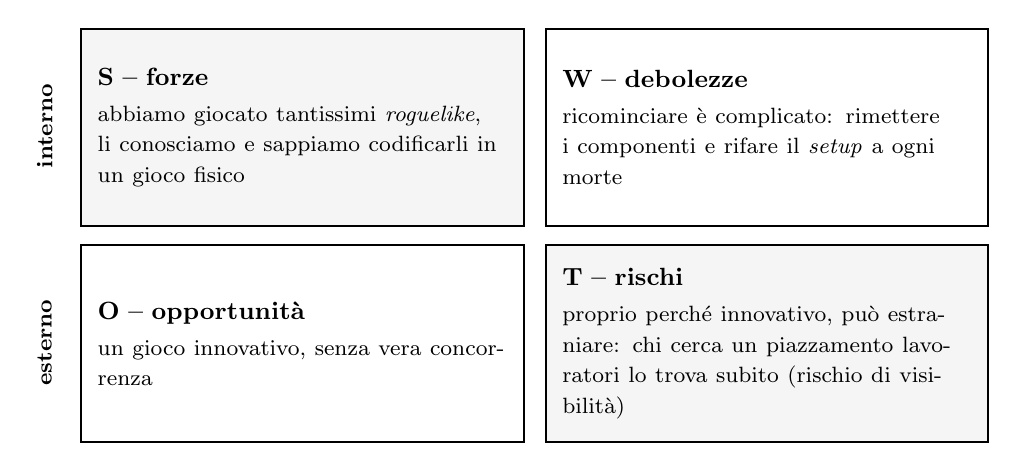
\begin{tikzpicture}[
  font=\small,
  a14q/.style={draw, thick, text width=5.2cm, minimum height=2.5cm, align=left,
               inner sep=6pt, anchor=north west}
]
  \node[a14q, fill=gray!8] (S) at (0,0) {\textbf{S -- forze}\\[2pt]\footnotesize abbiamo
    giocato tantissimi \emph{roguelike}, li conosciamo e sappiamo codificarli in un gioco
    fisico};
  \node[a14q] (W) at (5.9,0) {\textbf{W -- debolezze}\\[2pt]\footnotesize ricominciare è
    complicato: rimettere i componenti e rifare il \emph{setup} a ogni morte};
  \node[a14q] (O) at (0,-2.75) {\textbf{O -- opportunità}\\[2pt]\footnotesize un gioco
    innovativo, senza vera concorrenza};
  \node[a14q, fill=gray!8] (T) at (5.9,-2.75) {\textbf{T -- rischi}\\[2pt]\footnotesize
    proprio perché innovativo, può estraniare: chi cerca un piazzamento lavoratori lo
    trova subito (rischio di visibilità)};
  \node[rotate=90, font=\footnotesize\bfseries] at (-0.45,-1.25) {interno};
  \node[rotate=90, font=\footnotesize\bfseries] at (-0.45,-4.0) {esterno};
\end{tikzpicture}
\caption{L'analisi SWOT ``fatta in 30 secondi'' da Marta sull'esempio di un
\emph{roguelike} da tavolo. La riga in alto riguarda il progetto, quella in basso il mercato
di riferimento, inteso in senso largo (anche le persone che consultano itch.io). Le
categorie si leggono poi a coppie.}
\label{a14:fig:swot}
\end{figure}

\paragraph{Uno strumento si impara usandolo.} Ogni strumento visto oggi diventa più utile
\textbf{quanto più spesso lo si usa}. ``Non so se vi dilettate in cucina'', ma ci sono
tantissimi strumenti per cucinare, e più si usa uno strumento, più se ne conoscono limiti e
forze. Vale anche per la SWOT: ``la prima volta che la farete sarà una roba un po'
posticcia''; poi, man mano che la si sfrutta, si scoprono le sue utilità, soprattutto nel
\textbf{riassumere in breve} questi quattro punti.

% ---------------------------------------------------------------------
\section{Le \emph{personas}}
\label{a14:sec:personas}

\slidefig{img/AGD/agd14-personas}{Un esempio di persona.}{slide \emph{Tecniche di sviluppo}}{fig:agd14-personas}


Un altro strumento ``molto utile, sempre un po' mutuato da altri campi'', sono le
\textbf{\emph{personas}}, già accennate parlando di \emph{target}. ``Queste le conoscete?''
``Di nome, ma meno.''

\paragraph{Dal \emph{target} a una persona.} Quando si fa un gioco si ha in mente un
\emph{target}, ma i \emph{target} sono \textbf{misure astratte}: si può dire che un gioco è
``per gli appassionati'', ma ``se io dico appassionati, non ho in mente una persona''. Aiuta
invece avere \textbf{riferimenti molto specifici}. Siccome è difficile pensare in concreto a
una persona precisa che vuole il nostro gioco, si può ricorrere alle \emph{personas}, che
sono ``niente di più che'' \textbf{profili creati da noi}, popolati il più possibile.
Generalmente si costruiscono partendo da \textbf{dati molto generici} e poi
\textbf{scendendo nei dettagli}, stabilendo sempre di più i tratti di questa persona virtuale.

\paragraph{L'esempio della slide.} Nell'esempio della slide non c'è niente che non sia
definito in modo certo: la persona ha un \textbf{nome}\footnote{Nella trascrizione il nome è
prima ``Tian'' e poi ``Diane''; l'occupazione è ``e share consultant'', forse \emph{HR
consultant}. La slide non è nella trascrizione e il capitolo non può verificarlo.},
un'\textbf{età} (48 anni), un'\textbf{occupazione} (una consulente) e una \textbf{biografia},
una \emph{backstory} che racconta le cose che fa ogni giorno. Che cosa c'entrano con un gioco
da tavolo? ``Tendenzialmente, di base, niente.'' Ma anche per una persona reale le cose che fa
nella vita c'entrano poco con i suoi hobby; eppure ci aiutano a immaginare \textbf{che cosa
farebbe quella persona seduta a un tavolo da gioco}. Costruire una \emph{persona} dà una
dimensione e permette di \textbf{rispondere a delle domande}, del tipo: ``Diane giocherebbe
a \emph{I Coloni di Catan}?''\footnote{Nella trascrizione ``colonie di Katan''.} Più la
\emph{persona} è definita, più è probabile riuscire a rispondere.

\paragraph{Il rischio dei \emph{bias}.} Per la SWOT come per le \emph{personas}, il rischio è
che \textbf{i propri \emph{bias} condizionino il lavoro}. ``È un rischio che c'è sempre.''
L'invito è a essere persone \textbf{aperte} il più possibile, \textbf{curiose}, e a
\textbf{conoscere più persone possibile}: dà un vantaggio, e aiuta a calarsi negli altri con
più facilità.

\paragraph{\emph{Personas} costruite sui dati.} A seconda dell'entità del progetto, si possono
\textbf{raccogliere dei dati} e costruire le \emph{personas} su quei dati: fare dei campioni
quantitativi, per esempio con \textbf{un sondaggio}, per capire abitudini diffuse e interessi
condivisi di un certo \emph{target}. ``Magari a volte vi è capitato di fare un sondaggio'' che
chiedeva ``sei appassionata di giochi da tavolo?'' e poi ``quali libri leggi?'': ``e tu dici:
ok, ma che c'entra?''. A volte serve proprio a costruire questi profili.

\paragraph{Riusarle o no?} Uno degli inviti che si leggono spesso è a \textbf{non usare le
stesse \emph{personas} per più di un progetto}. Marta non la trova una regola necessariamente
funzionale: le è capitato di riusare le stesse \emph{personas} per più progetti, ``e
sinceramente non capisco bene il perché di no''. Riporta comunque quello che ha letto quando
ha imparato la tecnica: ognuno veda se gli torna utile.

\paragraph{Approfondimento: \emph{personas} e modelli di pubblico.} Bateman e Boon partono da
un modello di pubblico ancora più grezzo di quello che Marta chiama ``gli appassionati'': la
divisione tra giocatori \emph{hardcore} e \emph{casual}, che definiscono una ``ipotesi
consensuale'', accettata da quasi tutti nell'industria ma senza una definizione formale. Il
loro esempio è \emph{Resident Evil} per GameCube, che all'inizio chiedeva al giocatore se
preferisse ``scalare la montagna'' (oltre le fatiche c'è il risultato) o ``fare
un'escursione'' (la meta si raggiunge comodamente), per regolare la difficoltà. Le
\emph{personas} fanno il passo successivo: invece di due etichette, una persona con un nome,
un'età e una giornata, a cui fare domande concrete.

% ---------------------------------------------------------------------
\section{I sei cappelli per pensare}
\label{a14:sec:cappelli}

\slidefig{img/AGD/agd14-cappelli}{I sei cappelli per pensare.}{slide \emph{Tecniche di sviluppo}}{fig:agd14-cappelli}


``I sei cappelli per pensare. Questa forse la conoscete anche dal \emph{design}''. Qualcuno
l'ha sentita nominare; una voce, probabilmente di una studentessa, ricorda che nei suoi studi di \emph{design} se ne
parlava, ``ma non tramite i cappelli colorati'': il processo creativo analizzato da altri
punti di vista, ``però è molto interessante anche così''.

\paragraph{La prima pausa.} A questo punto Marta resta bloccata fuori dalle slide: ha aperto
la chat di Zoom e non riesce più a tornare alla presentazione (``vi giuro che non sono mai
stata così in difficoltà'', ``ho anche una laurea in informatica''; ``e ho fatto l'errore di
aprire la chat, non lo farò mai più''). Gli studenti continuano a vedere le slide, ma lei non
riesce a farle avanzare, e propone \textbf{dieci minuti di pausa} per risolvere. La pausa,
nella trascrizione, è coperta da frasi ripetute senza senso. Al ritorno: ``nel frattempo ho
trovato il modo di aprire la chat senza distruggere mezzo computer''.

\paragraph{A che cosa servono.} I sei cappelli sono un altro dei processi per
\textbf{calarsi in panni che non sono i propri}, utili soprattutto per figurarsi prospettive
che non sono quelle che vengono ``di primo acchito'' quando si lavora a un progetto. I
cappelli guardano a problemi simili \textbf{da punti di vista diversi}, e alcuni sono
volutamente \textbf{opposti}. Si possono usare in molti modi; Marta, per esempio, ha
\textbf{un mazzetto di sei carte}: le mescola, ne estrae una e si mette figurativamente quel
cappello. Si possono usare anche \textbf{in \emph{team}}: ognuno indossa un cappello, e poi
i cappelli \textbf{ruotano} per cambiare punto di vista. La tabella~\ref{a14:tab:cappelli}
li riassume.

\begin{description}
  \item[Il bianco: i fatti.] Guarda le cose \textbf{da un punto di vista neutrale}: asserisce
        i fatti nel modo più oggettivo possibile, si astiene dai giudizi e dà informazioni
        ``il più possibile dritte''. Per esempio: ``durante il \emph{playtest} è successa
        questa cosa'', senza dire se è positiva o negativa; ``si è verificato un paio di
        volte questo avvenimento''. Prende i dati in modo \textbf{distaccato}.
  \item[Il nero: i rischi.] Fa leva su \textbf{difficoltà, insicurezze, pericoli}: tutto
        quello che potrebbe non essere andato o potrebbe non andare. È uno dei cappelli
        \textbf{più facili da indossare}, perché è facile vedere le parti negative di un
        progetto. Proprio per questo invita a essere \textbf{più descrittivi}: non limitarsi
        a dire qual è la difficoltà, ma esplorarla e analizzarla nel dettaglio.
  \item[Il rosso: le emozioni.] Fa riferimento alle \textbf{emozioni}: come ci si sente
        quando lo si indossa, quali emozioni sono state provate. A differenza del nero,
        \textbf{non dà spiegazioni}: dice ``io mi sento così''. È un cappello molto utile e
        \textbf{spesso sottovalutato}, perché c'è la credenza che le emozioni valgano meno
        dei fatti; in realtà le emozioni guidano a capire qual è \textbf{l'esperienza
        desiderata}, che cosa si vuole ottenere da un \emph{design}, e se il \emph{design} lo
        sta facendo emergere.
  \item[Il giallo: i punti di forza.] È l'opposto del nero: elenca \textbf{le cose positive},
        i punti di forza, gli aspetti che esaltano l'esperienza. Anche questo è abbastanza
        semplice da indossare; anche qui l'invito è a ``lasciarsi andare'' sulle
        \textbf{ragioni} per cui quei punti sono di forza, e a sviscerarle.
  \item[La creatività.] Uno dei due cappelli ``più particolari''\footnote{Marta non dice il
        colore di questo cappello. Nel metodo originale di Edward de Bono (\emph{Six Thinking
        Hats}, 1985) il cappello della creatività è il \textbf{verde}.}: significa
        \textbf{lanciarsi in soluzioni anche esagerate e irrealistiche}. È il cappello del
        \textbf{\emph{brainstorming}}: si analizzano le possibilità, anche quelle fuori dagli
        schemi. Non importa se sono fattibili: il lavoro della creatività è \textbf{proporre
        idee}, soluzioni, possibilità; pensare a quali e quante sono, e cercare quelle più
        inusuali.
  \item[Il blu: l'organizzazione.] Il più particolare. In \emph{team} serve a
        \textbf{gestire gli altri cappelli}: chi indossa il blu stabilisce quando si cambia
        cappello. E inoltre dice: ``ok, però che cosa faremo? Che cosa implementeremo? Che
        cosa serve adesso per raggiungere gli scopi che ci prefiggiamo?''. È la parte
        \textbf{organizzativa} del processo, quella che segue la parte pratica una volta
        individuate le caratteristiche.
\end{description}

Nel complesso, i cappelli sono anche un modo di \textbf{dividere i pensieri in compartimenti
stagni}, ``e a volte questa cosa torna particolarmente utile''.

\begin{table}[htbp]
\centering
\small
\begin{tabular}{@{}p{2.3cm}p{3.6cm}p{3.9cm}p{3.7cm}@{}}
\toprule
\textbf{Cappello} & \textbf{Guarda a} & \textbf{Esempio di frase} & \textbf{Attenzione} \\
\midrule
Bianco & i fatti, neutri & ``durante il \emph{playtest} è successo due volte X'' & niente
  giudizi \\
\addlinespace
Nero & difficoltà, insicurezze, pericoli & ``questo potrebbe non funzionare perché\ldots'' &
  facile da indossare: va approfondito \\
\addlinespace
Rosso & le emozioni & ``io mi sento così'' & niente spiegazioni; spesso sottovalutato \\
\addlinespace
Giallo & i punti di forza & ``questo esalta l'esperienza perché\ldots'' & facile: andare a
  fondo delle ragioni \\
\addlinespace
Creatività (verde) & idee e soluzioni, anche irrealistiche & ``e se\ldots?'' & non giudica
  la fattibilità \\
\addlinespace
Blu & l'organizzazione: quando cambiare, che cosa fare ora & ``che cosa implementiamo?'' &
  in \emph{team}, gestisce gli altri \\
\bottomrule
\end{tabular}
\caption{I sei cappelli per pensare come li presenta Marta. Si possono pescare da un mazzetto
di sei carte, da soli, o far ruotare in un \emph{team}.}
\label{a14:tab:cappelli}
\end{table}

% ---------------------------------------------------------------------
\section{Il bilanciamento secondo Garfield}
\label{a14:sec:garfield}

\slidefig{img/AGD/agd14-bilancia}{Il bilanciamento.}{slide \emph{Tecniche di sviluppo}}{fig:agd14-bilancia}


``Ecco, ce l'ho fatta'': la slide successiva è il \textbf{bilanciamento}. ``Questo è il capitolo
un po' più complicato da fare, ma vedremo perché.'' Marta raccomanda di interromperla con le
domande, perché è ``un argomento molto spesso spinoso'', e lei lo tratta ``in un modo un po'
atipico rispetto ai miei colleghi''.

\paragraph{\emph{The Balancing Act}.} Si parte da uno degli articoli che da qualche anno sono
diventati un punto di riferimento per il suo lavoro, scritto ``niente di meno che'' da
\textbf{Richard Garfield}\footnote{Marta cita il titolo dell'articolo, \emph{The Balancing
Act}, ma non dice dove sia stato pubblicato; il capitolo non lo ha verificato. Le citazioni
che seguono sono la parafrasi italiana di Marta dalla slide, non il testo originale.}. Lo si
troverà citato spesso: Garfield è un designer con un'esperienza ormai
\textbf{quarantennale} (``ormai sono 40 anni, direi''), con tantissimi giochi di successo,
``non c'è solo \emph{Magic}'', e ha una profonda conoscenza non solo del gioco ma di tutto
ciò che gli ruota attorno. ``Secondo me è un'ottima lettura a prescindere'': molto spesso è
stato \textbf{sottovalutato}, perché molti lo associano solo a \emph{Magic}, ``e invece ha
fatto tanto, tanto di più''. Nell'articolo Garfield esorta così:
\begin{quote}
\textbf{il bilanciamento perfetto dei giochi è un mito. Il bilanciamento consiste nel
migliorare il \emph{play}, il giocare, per un ampio spettro di possibili giocatori, e
comporta costi e benefici.}
\end{quote}
È una frase che, per Marta, riassume perfettamente tanti punti del bilanciamento. La parte che
molti dimenticano è quella dei \textbf{costi e benefici}: qualsiasi bilanciamento si operi
presenterà, ``se vogliamo, anche per ricondurci all'analisi SWOT'', delle forze, delle
debolezze, delle opportunità e dei rischi.

\paragraph{Un'esplorazione dello spazio di gioco.} Che cos'è, allora, il bilanciamento? Si
può definire come \textbf{l'esplorazione di una parte dello spazio di gioco totale}. Dato un
gioco, applicando bilanciamenti diversi, e anche regole diverse, se ne esplora una parte
diversa. Quando si presenta un gioco sviluppato, finito, si sta implicitamente consegnando
\textbf{una porzione di uno spazio di gioco molto più ampio} (figura~\ref{a14:fig:spazio}).

\paragraph{Non esiste un bilanciamento che accontenti tutti.} Si pensa che questa porzione
debba accontentare tutti, ma, proprio per i costi e benefici, non è così. Molto spesso chi
segue il principio di accontentare tutti \textbf{sta accontentando soltanto la parte più
rumorosa dell'utenza}: quella che si esprime in modo più vocale, spesso non da una posizione
di conoscenza, ma perché è molto facile giudicare un gioco; e ``quindi molto spesso si
prendono dei granchi''. \textbf{Abbandonare l'idea che un gioco possa risultare adatto a
chiunque} è, per Marta, l'obiettivo da avere quando ci si mette sotto con lo sviluppo: ``non
esistono giochi che sono adatti a tutte le persone''.

\begin{figure}[htbp]
\centering
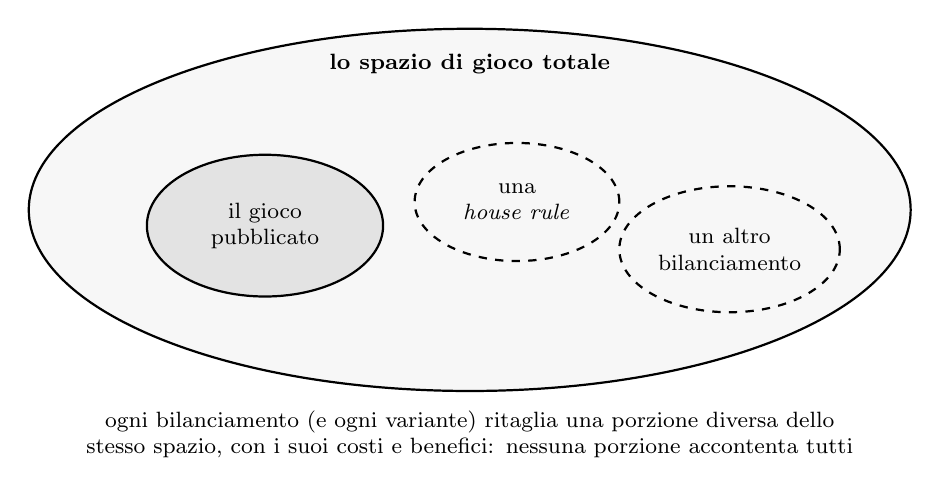
\begin{tikzpicture}[font=\small]
  \draw[thick, fill=gray!6] (0,0) ellipse (5.6cm and 2.3cm);
  \node[font=\footnotesize\bfseries] at (0,1.85) {lo spazio di gioco totale};
  \draw[thick, fill=gray!22] (-2.6,-0.2) ellipse (1.5cm and 0.9cm);
  \node[align=center, font=\footnotesize] at (-2.6,-0.2) {il gioco\\pubblicato};
  \draw[thick, dashed] (0.6,0.1) ellipse (1.3cm and 0.75cm);
  \node[align=center, font=\footnotesize] at (0.6,0.1) {una\\\emph{house rule}};
  \draw[thick, dashed] (3.3,-0.5) ellipse (1.4cm and 0.8cm);
  \node[align=center, font=\footnotesize] at (3.3,-0.5) {un altro\\bilanciamento};
  \node[font=\footnotesize, text width=10cm, align=center] at (0,-2.85) {ogni bilanciamento
    (e ogni variante) ritaglia una porzione diversa dello stesso spazio, con i suoi costi e
    benefici: nessuna porzione accontenta tutti};
\end{tikzpicture}
\caption{Il bilanciamento come esplorazione dello spazio di gioco: il gioco finito ne
consegna una porzione; le \emph{house rules} e le varianti, nell'analogico, permettono a chi
gioca di esplorarne altre.}
\label{a14:fig:spazio}
\end{figure}

\paragraph{Dare più potere a chi gioca.} Il mondo analogico ha una grande forza che nel
videogioco non è altrettanto facile: \textbf{se vogliamo cambiare una regola, basta dirlo
quando si spiegano le regole}. Nel videogioco, per farlo, servono di solito conoscenze di
programmazione o di progettazione che vanno al di là di quello che l'utenza comune riesce a
fare. Il gioco analogico dà invece uno strumento molto forte: \textbf{varianti} e
\textbf{\emph{house rules}}, per tarare il gioco sul proprio livello.

\paragraph{Il gioco non è un artefatto immutabile.} Marta spende ``altre due parole''. C'è una
tendenza, che lei stessa ha seguito per tanti anni, a pensare al gioco come a un
\textbf{artefatto immutabile}: è stato fatto così e non può essere toccato. Esiste in molti
ambiti, per esempio con i libri, che molte persone non vogliono assolutamente modificare,
segnare, sottolineare. È una concezione che Marta si prende la libertà di definire ``molto
orientata al capitalismo'', in cui gli oggetti non sono davvero propri ma entità da
preservare per preservarne il valore. I \textbf{giochi \emph{legacy}} aiutano a svincolarsi
da questo principio. \textbf{Lavorare su un gioco e metterci del proprio è il gesto di
possesso più forte che si possa fare}, e in un certo senso anche un gesto d'amore: se si
modifica un gioco con \emph{house rules} e varianti, probabilmente è perché piace così tanto
che, piuttosto che bollarlo come ``non è un gioco per me'', si è disposti a
\textbf{esplorarne lo spazio di gioco}. È una cosa che nell'ambiente si è un po' persa, ma
che è sempre stata una caratteristica del gioco: Marta invita a riscoprirla, ``perché tira
fuori tante cose positive''.

\paragraph{Le \emph{house rules} come palestra di sviluppo.} Inoltre, praticare le \emph{house
rules} \textbf{spinge verso lo sviluppo}: toccare un gioco edito e vedere come cambia variando
le regole trasmette il \emph{feeling} di lavorare a un gioco già creato da qualcun altro e
metterci le mani sopra, cioè proprio il mestiere di chi sviluppa.

\paragraph{L'obiettivo: esaltare le forze, minimizzare gli ostacoli.} L'obiettivo del
bilanciamento è lo stesso dello sviluppo in generale: \textbf{esaltare le forze del
\emph{design} e minimizzare gli ostacoli}. Non lo si pensi come il raggiungimento di un
\textbf{equilibrio perfetto}, che non esiste; ci si chieda sempre: ``ok, però questo
\emph{design} che cosa si promette di fare? Come faccio a veicolarlo?''.

% ---------------------------------------------------------------------
\section{Per chi si bilancia}
\label{a14:sec:perchi}

È importante ricordare \textbf{per chi} si sta facendo il bilanciamento. Potrebbero essere
persone \textbf{esperte}, appassionate; persone \textbf{alle prime armi}; o, a volte, ``il
\textbf{dio della simmetria}'', come lo chiamano dove lavora Marta.

\paragraph{Il dio della simmetria.} È quando ci si intestardisce che \textbf{i numeri debbano
finire tutti per 5 o per 10}, o che, siccome questa carta vale 2, \textbf{anche quella debba
valere 2}, senza contemplare per esempio i numeri dispari: ``sono tutte delle fisime che vengono
fuori quando si sviluppa''\footnote{Nella trascrizione ``sono tutte delle fisiche'': quasi
certamente ``fisime''.}. ``Io sono la prima che a volte ci cade, in questi tranelli'': l'ha
messo nella slide anche per prendersi in giro. Ma è un avvertimento serio: quando si bilancia,
si tende verso i propri \emph{bias}, e il dio della simmetria è uno di questi.

\paragraph{Bilanciare per il gioco.} A volte si bilancia \textbf{per il gioco}, cioè per il suo
interesse: il gioco vuole creare certe dinamiche, quelle infuse da chi l'ha creato, e
bilanciare per il gioco significa \textbf{non pensare necessariamente al \emph{target}}, ma a
come tirare fuori il più possibile l'esperienza. Vale soprattutto per i \textbf{giochi non
commerciali}, in cui l'interesse è portare l'esperienza anche a discapito dell'utenza, e per
i giochi \textbf{molto sperimentali}.

L'esempio è un gioco ``molto bello'' di \textbf{Amabel Holland}, in solitario, che si chiama
\textbf{\emph{Endurance}}\footnote{Il titolo e l'autrice sono detti chiaramente; editore e
anno non sono nominati. Amabel Holland pubblica di solito con Hollandspiele.}. Ricrea le
vicende della spedizione dell'\emph{Endurance}, ``una spedizione miracolosa'' in cui i membri
dell'equipaggio si sono salvati dopo una quantità immensa di tempo passato, ``se non
sbaglio'', in Antartide\footnote{È la spedizione imperiale transantartica di Ernest
Shackleton (1914--1917): la nave \emph{Endurance} rimase intrappolata nei ghiacci e affondò,
e tutto l'equipaggio sopravvisse dopo quasi due anni.}. Quello che Holland ha voluto ricreare
è che, quando si gioca, \textbf{nel 99\% dei casi si perde}, perché l'equipaggio muore.
``Perdere'' è un'imprecisione: nel gioco \textbf{non ci sono vere condizioni di vittoria o di
sconfitta}, ma un'analisi di quello che è successo e un racconto dell'esperienza. La storia in
cui tutti si salvano è \textbf{volutamente rarissima}, per dimostrare la straordinarietà
dell'evento reale e ricalcare la difficoltà di ottenere un risultato del genere. Qui si
bilancia per il gioco, anche se il \emph{target} potrebbe non apprezzarlo; o meglio, c'è un
\emph{target} ``un po' più nascosto'' di quello commerciale.

\paragraph{Bilanciare per il \emph{target}.} È il discorso inverso: si bilancia per chi,
secondo noi, giocherà il gioco. Tendenzialmente si bilancia per il \emph{target}, ma nella
pratica è più difficile di quanto sembri, perché è facile \textbf{dimenticare che si sta
bilanciando per persone con interessi diversi dai nostri}, e finire a bilanciare per noi
stessi. L'esempio che aiuta è quello dei \textbf{giochi per bambini}: lì ``chiaramente noi non
siamo bambini'', e la differenza salta all'occhio. Quando Marta ha lavorato a un gioco per
bambini chiamato \textbf{\emph{Sun Farm}}\footnote{Così nella trascrizione; il titolo non è
verificabile.}, il bilanciamento è partito \textbf{dai bambini e dai genitori}: capire quale
potesse essere l'esperienza desiderata da un bambino, e perché in quel caso \textbf{vincere
non era la cosa più importante dell'universo}, mentre contavano di più
l'\textbf{espressività} e la possibilità di giocare un po' con le strategie senza restringere
il campo delle possibilità.

\paragraph{Esperti o principianti.} C'è spesso la tendenza a fare giochi \textbf{solo per i
giocatori migliori}, o per quelli che sono vocali e si spacciano per i migliori. Molto spesso
sono persone che \textbf{il gioco l'hanno giocato pochissimo}: sui gruppi e sui \emph{forum}
si trovano persone che dicono ``questo gioco è rotto'' dopo una partita. È una tendenza che
c'è anche \textbf{nell'industria}, dietro le quinte, tra addetti ai lavori; ``posso ammettere
che anche io l'ho fatto''. Ed è, come dice anche Garfield, \textbf{profondamente
irrispettoso}: si pensa che il gioco sia fatto solo per noi, quando magari non siamo
minimamente nel suo \emph{target}, o il gioco richiede competenze che non abbiamo o non
abbiamo voglia di applicare. Bisogna ricordarsi che \textbf{un gioco non è giocato soltanto
da queste persone}: è giocato da tantissime persone che non commentano sui \emph{forum}, non
scrivono su BGG, non lasciano voti. E il gioco deve essere \textbf{accessibile al maggior
numero possibile di persone}, proprio perché arrivi anche nelle mani di chi non si esprime ma
avrebbe piacere di giocarlo.

\paragraph{Tecnicità contro approcciabilità.} Per riassumere: da una parte si bilancia
\textbf{per tecnicità}, per rendere il gioco ``più bello'', e magari non si riesce ad
accontentare nessuno, perché per $N$ persone che si lamentano ce ne saranno $M$ che si
lamenteranno una volta fatta la modifica. Dall'altra si bilancia \textbf{per
approcciabilità}, per rendere il gioco più approcciabile: questo \textbf{allarga la base
d'utenza} che può accedere al gioco e favorisce che venga effettivamente provato. Marta
precisa, ``fatemi sapere se non vi è chiara la differenza'': \textbf{non significa che non si
possano fare giochi complessi}, o impegnativi. ``Non è questo il punto del discorso.''

% ---------------------------------------------------------------------
\section{Perché non bilanciare (solo) con la matematica}
\label{a14:sec:matematica}

Perché, allora, non si bilancia spesso \textbf{``in modo matematico''}, come si dice? Marta
elenca le ragioni.

\paragraph{È lungo e soggetto a errori.} Non conosce le competenze matematiche di tutte le
persone che si avvicinano al \emph{design} e allo sviluppo, ma nella sua esperienza vede
molto spesso \textbf{ragionamenti matematici fallaci}, che ``non stanno in piedi''. Ed è un
processo \textbf{lungo e faticoso}, che porta a sbagliare tantissime volte. A meno di essere
``davvero, davvero, davvero molto in gamba'' su questo aspetto, va affrontato con cautela.

\paragraph{È difficilmente modellabile.} Molto spesso \textbf{i modelli sono sbagliati}:
quando si cerca di sintetizzare un gioco si perdono \textbf{le dipendenze tra le risorse}, le
\textbf{transazioni} da una risorsa all'altra, da una carta all'altra. E si perde quello che
rende i giochi affascinanti: i cosiddetti \textbf{spazi di permeabilità}, già nominati
``ieri'', che \textbf{neanche il designer conosce sempre in modo approfondito} e che fanno la
differenza. I giochi sono interessanti proprio perché sono sistemi \textbf{non pienamente
controllati, non pienamente compresi}. Si pensi agli \textbf{scacchi}: chi li ha progettati
non aveva ``minimamente idea'' di tutto quello che è venuto dopo; molte innovazioni
strategiche sono degli ultimi cinquant'anni. È notevole quanti spazi di permeabilità avesse,
grazie alla struttura aperta del suo albero decisionale, ``che, penso lo sapete, è
immenso''.

\paragraph{Appiattisce le scelte.} Bilanciare in modo matematico porta a un
\textbf{appiattimento delle scelte}, perché si tende a trovare degli \textbf{equilibri
statici}: si immagini una bilancia perfettamente in equilibrio. Ne nascono le famose
\textbf{scelte indifferenti}: qualsiasi cosa si faccia, la ricompensa è identica. Un percorso
dà 1 punto vittoria al primo turno, 3 al secondo e 2 al terzo; un altro ne dà 1 al primo, 2 al
secondo e 3 al terzo. Alla fine \textbf{sono 6 punti per tutte e due le strade}: ``quindi
abbiamo risolto assolutamente niente'' (figura~\ref{a14:fig:indifferenti}). L'esperienza
diventa \textbf{statica e priva di significato}.

\begin{figure}[htbp]
\centering
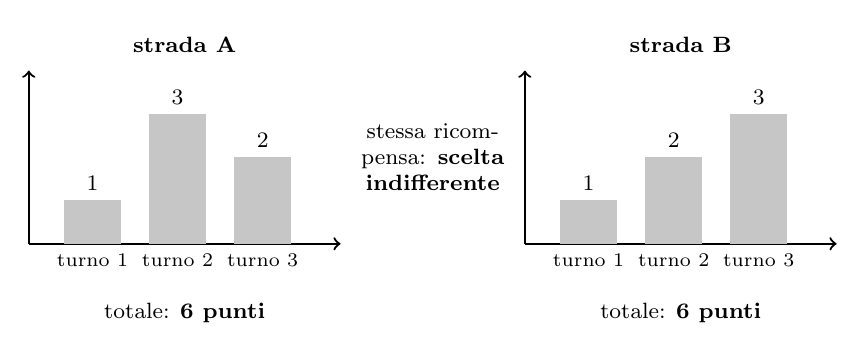
\begin{tikzpicture}[font=\small, x=0.9cm, y=0.55cm]
  % assi
  \foreach \ox/\tit/\a/\b/\c in {0/{strada A}/1/3/2, 7/{strada B}/1/2/3}{
    \draw[thick, ->] (\ox,0) -- (\ox+4.4,0);
    \draw[thick, ->] (\ox,0) -- (\ox,4.0);
    \node[font=\footnotesize\bfseries] at (\ox+2.2,4.6) {\tit};
    \fill[gray!45] (\ox+0.5,0) rectangle (\ox+1.3,\a);
    \fill[gray!45] (\ox+1.7,0) rectangle (\ox+2.5,\b);
    \fill[gray!45] (\ox+2.9,0) rectangle (\ox+3.7,\c);
    \node[font=\footnotesize, above] at (\ox+0.9,\a) {\a};
    \node[font=\footnotesize, above] at (\ox+2.1,\b) {\b};
    \node[font=\footnotesize, above] at (\ox+3.3,\c) {\c};
    \node[font=\scriptsize, below] at (\ox+0.9,0) {turno 1};
    \node[font=\scriptsize, below] at (\ox+2.1,0) {turno 2};
    \node[font=\scriptsize, below] at (\ox+3.3,0) {turno 3};
    \node[font=\footnotesize] at (\ox+2.2,-1.6) {totale: \textbf{6 punti}};
  }
  \node[font=\footnotesize, text width=2.4cm, align=center] at (5.7,2.0) {stessa
    ricompensa: \textbf{scelta indifferente}};
\end{tikzpicture}
\caption{L'esempio di Marta di scelte indifferenti, prodotto da un bilanciamento matematico
``statico'': due percorsi con andamenti diversi ma lo stesso totale. Scegliere l'uno o
l'altro non cambia niente.}
\label{a14:fig:indifferenti}
\end{figure}

``Anche qua'', precisa, ``non significa che non si usa la matematica'': la matematica aiuta e
può tornare comoda sotto molti aspetti. Ma bisogna fare attenzione a \textbf{non guardare il
bilanciamento solo da questo punto di vista}, perché è una tendenza comune a chi si avvicina al
bilanciamento e porta a degli errori.

\paragraph{Il bilanciamento esperienziale.} Marta consiglia sempre il \textbf{bilanciamento
esperienziale}: veicolare \textbf{i percorsi intesi}, l'obiettivo del \emph{design}. Che cosa
si prefigge il gioco? Quali strade voglio che siano percorse a livello strategico? Che cosa
voglio \textbf{premiare}? Costruire le \textbf{scelte sensibili}, cioè indirizzare le scelte
delle persone verso alcune delle idee e delle strategie che si vogliono mettere in campo, e
lasciare che il \emph{gameplay} sia \textbf{emergente}, che consenta anche a chi gioca di
metterci del proprio. Il bilanciamento esperienziale è anche \textbf{parametrizzabile}: se tra
gli \emph{stakeholder} c'è chi vuole un gioco ``un po' più cattivo'', che restituisca un
\emph{feeling} di frustrazione, lo si può fare senza problemi; il bilanciamento matematico
molto spesso lo impedisce, perché tende a equalizzare tutto su un livello statico.

\paragraph{E l'intelligenza artificiale?} Un tema diventato rilevante quest'anno, ``l'anno
scorso lo era un po' meno'': molte persone \textbf{bilanciano con l'intelligenza
artificiale}. Marta non si mette a spiegare come funziona, ``però insomma, non è una cosa che
veramente pensi, mettiamola così: è semplicemente un \textbf{algoritmo predittivo}''. Molto
spesso porta proprio agli \textbf{errori del bilanciamento matematico}. Il suo invito è a
\textbf{non usarla}; ma chi la usa faccia attenzione, perché può portare a un bilanciamento
``assolutamente errato e che appiattisce il gioco''.

\paragraph{Approfondimento: il modello e il gioco.} Schell non è contrario ai modelli, ma ne
descrive bene il limite: ``il modello informa il bilanciamento, e il bilanciamento informa il
modello''. Si scrive il proprio modello di come sono legate le meccaniche, lo si mette alla
prova giocando, e lo si corregge ogni volta che il gioco non si comporta come previsto.
Aggiunge che il bilanciamento può cominciare davvero solo quando il gioco è giocabile, e che
la sua regola personale è dedicare al bilanciamento \textbf{metà del tempo di sviluppo}. È la
stessa direzione di Marta: i numeri servono, ma come ipotesi da verificare al tavolo, non come
risposta.

% ---------------------------------------------------------------------
\section{Come cominciare: giochi a scarsa interazione}
\label{a14:sec:cominciare}

Un consiglio per chi vuole iniziare a sperimentare con il bilanciamento: partire da
\textbf{giochi a scarsa interazione}. I giochi ad alta interazione hanno tante
\textbf{interdipendenze} con quello che fanno i giocatori; si possono modellare anche
matematicamente, soprattutto in termini probabilistici, ``ma è molto complesso''. Partire da
giochi con poca interazione permette di lavorare in modo più agevole. Marta precisa che sta
parlando soprattutto di giochi con \textbf{un modello matematico alle spalle}: giochi con
\textbf{conversioni di risorse}, in cui si vince a \textbf{punti vittoria}; non tanto di giochi
narrativi. Nel mondo del gioco da tavolo c'è ancora una preponderanza di questo tipo di giochi,
e quando si parla di bilanciamento si parla di solito di questo, anche se, come detto la volta
prima, non è affatto l'unico che si fa.

\paragraph{Modellare il sistema.} Partendo da un gioco a scarsa interazione, si prova a
\textbf{modellarne il sistema}: capire le \textbf{dipendenze} tra le risorse, con un
\textbf{diagramma di flusso} o anche un \textbf{diagramma di stato}, se torna utile.
L'obiettivo è individuare il \textbf{percorso che fanno le risorse}: quando vengono prese,
quando vengono restituite, e così via.

\paragraph{Un esempio: \emph{Splendor} infinito.} Si può partire da \textbf{\emph{Splendor}} e
immaginarlo con \textbf{risorse infinite}: le fiche di ogni colore sono infinite, e le carte
sono in $N$ copie, quindi possono essere sempre prese. Si prova a bilanciare da lì e si vede
che succede.

\paragraph{Variare i parametri.} Si testa come varia il gioco al variare dei parametri,
semplicemente \textbf{cambiando i parametri}, anche in modo arbitrario (tra poco si vedranno
alcune tecniche). Per esempio: che succede se, in \emph{Splendor}, una delle risorse, la
carta, diventa \textbf{esclusiva}, e non più in $N$ copie?

\paragraph{I \emph{test} in solitaria e il \emph{groupthink}.} I \emph{test} in solitaria qui
sono agevoli, ma attenzione al \textbf{\emph{groupthink}}, soprattutto se se ne fanno molti
durante il bilanciamento: ragionando da soli capita molto spesso di \textbf{rinforzare i
propri \emph{bias}}, e può diventare un problema, soprattutto se non si è consapevoli di
averli. Bisogna testare con \textbf{più persone}, e potenzialmente con \textbf{più gruppi
possibili}, per capire come si assesta il bilanciamento ed evitare il fenomeno.

\paragraph{Lasciare gli spazi di permeabilità.} ``Mi raccomando'': non bisogna avere
\textbf{l'ansia di controllare tutto il sistema di gioco}; non è necessario.

\paragraph{La strategia dominante emerge.} Se c'è una \textbf{strategia dominante}, di solito
la si intuisce analizzando il gioco da diversi punti di vista, o anche banalmente con i
\emph{playtest}: con un numero sufficiente di partite, i comportamenti emergono. L'esempio più
popolare: \textbf{tenere traccia di chi inizia a giocare} e vedere se è la persona che vince.
Se lo è, c'è un problema: chi inizia magari vince perché \textbf{fa un turno in più} degli
altri (``generalmente questo può essere uno dei motivi'').

% ---------------------------------------------------------------------
\section{Il budget di complessità}
\label{a14:sec:budget}

Uno dei concetti che tornano molto utili nello sviluppo, e che si trovano spesso soprattutto
nel bilanciamento, è il \textbf{budget di complessità}. Un gioco ha una certa complessità, un
certo grado di difficoltà: non la si immagini necessariamente come un numero, ma comunque come
\textbf{una quantità}, una quantità $x$. Quando si lavora al gioco, \textbf{rimuovere o
cambiare delle parti altera il budget}. Generalmente, togliendo per esempio una meccanica, si
\textbf{guadagna} complessità disponibile. E che cosa ci si fa, con questo guadagno?
\begin{itemize}
  \item lo si può semplicemente \textbf{togliere}, riducendo la complessità generale
        dell'esperienza;
  \item oppure lo si può \textbf{investire} altrove.
\end{itemize}

\paragraph{L'esempio del mercato azionario.} Si immagini un gioco con un obiettivo molto
definito: far sperimentare a chi gioca \textbf{come varia il mercato azionario}. Sul tavolo ci
sono i vari beni messi sul mercato, e bisogna rappresentare questo aspetto. Se il gioco ha
anche una \textbf{fase d'asta}, sta concentrandosi sull'asta: oltre ad aggiungere complessità,
\textbf{toglie \emph{focus}} alle fluttuazioni di mercato, cioè al comprare e vendere.
Togliendo l'asta si riduce la complessità; e quello che si è guadagnato lo si può usare per
rendere \textbf{un po' più complessa} la parte del mercato: il comprare, il vendere, il variare
dei prezzi dei beni. Il gioco diventa \textbf{più focalizzato}, più centrato su ciò che vuole
rappresentare, al prezzo di aver tolto una meccanica, ma \textbf{senza aver necessariamente
ridotto il budget di complessità} (figura~\ref{a14:fig:budget}).

\paragraph{Nel dubbio, accessibile.} Se non si intuisce che c'è qualcosa da fare con la
complessità recuperata, ``chiaramente sappiate che è sempre meglio avere un gioco
\textbf{accessibile} laddove è possibile'': lo scoglio iniziale, cioè provare il gioco e
metterlo sul tavolo, diventa più semplice.

\begin{figure}[htbp]
\centering
\begin{tikzpicture}[font=\small, x=1cm, y=1cm]
  % prima
  \node[font=\footnotesize\bfseries] at (1.0,4.5) {prima};
  \draw[thick] (0,0) rectangle (2,4);
  \fill[gray!20] (0,0) rectangle (2,1.6);
  \node[font=\footnotesize] at (1,0.8) {asta};
  \fill[gray!45] (0,1.6) rectangle (2,3.6);
  \node[font=\footnotesize, align=center] at (1,2.6) {mercato};
  \node[font=\scriptsize] at (1,3.8) {altro};
  % opzione 1
  \node[font=\footnotesize\bfseries, align=center] at (5.2,4.5) {togliere e\\basta};
  \draw[thick] (4.2,0) rectangle (6.2,4);
  \fill[gray!45] (4.2,0) rectangle (6.2,2.0);
  \node[font=\footnotesize] at (5.2,1.0) {mercato};
  \node[font=\scriptsize] at (5.2,2.2) {altro};
  \node[font=\scriptsize, align=center] at (5.2,3.3) {budget\\libero};
  % opzione 2
  \node[font=\footnotesize\bfseries, align=center] at (9.4,4.5) {reinvestire\\nel focus};
  \draw[thick] (8.4,0) rectangle (10.4,4);
  \fill[gray!45] (8.4,0) rectangle (10.4,3.6);
  \node[font=\footnotesize, align=center] at (9.4,1.8) {mercato\\più ricco};
  \node[font=\scriptsize] at (9.4,3.8) {altro};
  \draw[-{Stealth[length=2.5mm]}, thick] (2.3,2) -- (3.9,2);
  \draw[-{Stealth[length=2.5mm]}, thick] (2.3,2.6) to[bend left=25] (8.1,2.6);
  \node[font=\footnotesize, text width=11cm, align=center] at (5.2,-0.7) {togliendo
    l'asta si libera complessità: la si può lasciare libera (gioco più accessibile) o
    spenderla dove il gioco vuole il suo \emph{focus}};
\end{tikzpicture}
\caption{Il budget di complessità nell'esempio di Marta del gioco sul mercato azionario.
L'altezza della colonna è il budget complessivo; i blocchi sono le parti del gioco che lo
consumano.}
\label{a14:fig:budget}
\end{figure}

% ---------------------------------------------------------------------
\section{Strategie ad alto e a basso rischio}
\label{a14:sec:rischio}

\slidefig{img/AGD/agd14-rischio}{Strategie ad alto e a basso rischio.}{slide \emph{Tecniche di sviluppo}}{fig:agd14-rischio}


Un altro concetto che torna spesso sono le \textbf{strategie ad alto e a basso rischio}. Quando
si bilancia, uno dei riferimenti può essere avere più strategie: alcune in cui si
\textbf{rischia tanto, ma la ricompensa è elevata}, e altre in cui il \textbf{rischio è
ridotto, ma la ricompensa è parziale}. È un esempio tipico di tecnica per creare
\textbf{scelte sensibili}: dove c'è una sola possibilità, creare questa \textbf{biforcazione}
aiuta a costruire una scelta, ``e per come è fatta funziona un po' sempre''.

\paragraph{Perché funziona.} La difficoltà sta nel \textbf{valutare il livello di rischio} e
quanto si vuole rischiare di volta in volta. E siccome noi umani \textbf{fatichiamo con il
calcolo delle probabilità}, questo nel gioco diventa una forza, ``una sorta di abilità che si
può allenare''. È uno degli strumenti da mettere a disposizione quando serve una dinamica con
\textbf{più strade per arrivare a un risultato}: due macro-strategie, una che lavora tendenzialmente
a basso rischio e una ad alto rischio. Le due strade \textbf{non sono separate}: magari ci sono
strategie definite, ma è sempre possibile \textbf{passare dall'una all'altra lungo il
percorso}, e questo crea una dinamica di gioco effettiva.

\paragraph{L'esempio su \emph{Splendor}.} Sempre partendo da \emph{Splendor}: posso prendere
\textbf{una carta senza vederla} da uno dei mazzi e \textbf{riservarmela in mano}. Potrebbe
essere una strategia ad alto rischio, ma magari è l'unico modo di arrivare a \textbf{un quarto
mazzo} con le ricompense più alte: perdo il turno rischiando di non trovare quello che mi
serve, ma intanto ho la possibilità di fare qualcosa che le altre carte non mi permettono.
Una strategia a basso rischio è invece giocare con quello che ho, magari con le carte del
primo livello\footnote{L'esempio è in parte ipotetico: in \emph{Splendor} si può davvero
riservare una carta a faccia in giù dalla cima di un mazzo (ricevendo un gettone oro), ma i
mazzi di sviluppo sono tre; il ``quarto mazzo'' con le ricompense più alte è un'aggiunta di
Marta per illustrare il principio.}.

\paragraph{Approfondimento: la triangolarità.} È la \emph{lente della triangolarità} di
Schell, già incontrata nella lezione precedente: offrire al giocatore la scelta tra una mossa
sicura a bassa ricompensa e una rischiosa ad alta ricompensa. Il suo esempio è \emph{Space
Invaders}: i nemici normali valgono pochi punti e sono facili da colpire, mentre la navicella
misteriosa che attraversa ogni tanto lo schermo vale molto di più, ma inseguirla espone al
pericolo. Schell aggiunge una domanda di controllo che si applica bene alla biforcazione di
Marta: il tentativo di triangolarità è bilanciato, cioè la ricompensa è commisurata al
rischio?

% ---------------------------------------------------------------------
\section{L'ancoraggio}
\label{a14:sec:ancoraggio}

\slidefig{img/AGD/agd14-ancoraggio}{L'ancoraggio.}{slide \emph{Tecniche di sviluppo}}{fig:agd14-ancoraggio}


Un'altra tecnica di bilanciamento è l'\textbf{ancoraggio}. Quando si vogliono bilanciare dei
valori, può essere utile vedere le risorse attraverso \textbf{un valore di riferimento}: c'è un
cosiddetto \textbf{valore ancora}, e \textbf{tutto il sistema viene rapportato a quel
valore}. Due avvertenze, perché la tecnica è molto matematica, molto legata alla gestione dei
numeri:
\begin{itemize}
  \item le \textbf{risorse interdipendenti} rischiano di non essere facili da modellare. Per
        esempio: quanto vale \textbf{un turno extra}, in termini di valore ancora? ``È un
        argomento un po' complesso, perché un turno quanto vale?'';
  \item attenzione ai \textbf{meccanismi autobilancianti}, come il \textbf{\emph{draft}} di
        carte, che molto spesso vanno in opposizione alla tecnica dell'ancoraggio.
\end{itemize}

\paragraph{Il caso \emph{Stone Age}.} Come si fa? Partendo da un gioco molto semplice,
\textbf{\emph{Stone Age}}. ``Non so se lo conoscete.'' Gli studenti non ricordano di averlo
visto a lezione. È un gioco ``abbastanza vecchio'', un classico \textbf{piazzamento
lavoratori}. La sua particolarità: si piazzano i propri omini sui vari spazi, e quando li si
riprende \textbf{si lanciano tanti dadi quanti omini} si sono usati per prendere quella risorsa.
Se, per esempio, sono il giocatore giallo e ho \textbf{4 omini sul legno}, li riprendo e lancio
\textbf{4 dadi}; sommo il risultato e lo \textbf{divido per 3}, cioè conto quante volte il 3 sta
nel numero che ho fatto: quelle sono le risorse legno che ottengo. \textbf{Con 4 dadi e un
totale di 9, ottengo 3 legni}.

\paragraph{Le capanne.} A un certo punto del gioco si possono costruire \textbf{le capanne}, che
danno un certo numero di punti, mostrati nella slide sotto le capanne. Marta fa notare (dopo
essersi corretta: ``oddio, scusate, ho fatto un errore'') che \textbf{il valore in punti di una
capanna è pari al suo costo di costruzione}: un legno vale 3, un altro legno 3, un oro 6, come
si vede dalla tabella; $3+3+6=12$, e questo è il valore della capanna. Da qui si intuisce che
\textbf{il valore ancora del gioco sono i puntini sul dado}: \textbf{un puntino sul dado equivale
a un punto vittoria}. Va convertito, perché non dà punti di per sé, ma è il valore a cui si
appoggia tutta la matematica sottesa del gioco. Infatti: $3+3+5=11$, $4+4+6=14$, e così via
(tabella~\ref{a14:tab:stoneage}). Ci sono anche \textbf{capanne con il punto interrogativo}:
quella della slide dice ``usa 5 risorse qualsiasi, ma di almeno 4 tipi diversi'', e il
punteggio è dato proprio dalla somma dei valori delle risorse spese. ``Quindi non è neanche così
nascosta, come informazione.''

\begin{table}[htbp]
\centering
\small
\begin{tabular}{@{}lcp{7.2cm}@{}}
\toprule
\textbf{Risorsa} & \textbf{Divisore = valore} & \textbf{Che cosa vuol dire} \\
\midrule
Cibo & 2 & (non usato per le capanne) \\
Legno & 3 & con 4 dadi e totale 9, si prendono 3 legni \\
Argilla & 4 & \\
Pietra & 5 & \\
Oro & 6 & la risorsa più ``cara'' da ottenere ai dadi \\
\midrule
\multicolumn{3}{@{}l}{\textbf{Capanne (punti = somma dei valori delle risorse spese)}} \\
\multicolumn{3}{@{}l}{legno + legno + oro: $3+3+6 = 12$} \\
\multicolumn{3}{@{}l}{legno + legno + pietra: $3+3+5 = 11$} \\
\multicolumn{3}{@{}l}{argilla + argilla + oro: $4+4+6 = 14$} \\
\multicolumn{3}{@{}l}{capanna ``?'' (5 risorse qualsiasi, almeno 4 tipi): la somma dei
  loro valori} \\
\bottomrule
\end{tabular}
\caption{L'ancoraggio in \emph{Stone Age}: il valore ancora è il puntino del dado (un puntino
= un punto vittoria), e ogni risorsa vale quanti puntini servono per ottenerla. I divisori di
cibo, argilla e pietra non sono detti nella lezione e sono quelli del gioco; Marta nomina
esplicitamente il 3 del legno e il 6 dell'oro.}
\label{a14:tab:stoneage}
\end{table}

\paragraph{Che cosa permette l'ancoraggio.} Con il valore ancora si possono progettare
\textbf{quante capanne si vogliono}, perché è facile capire il loro valore in punti vittoria; e
si può costruire tutta la matematica del gioco, per esempio il valore di una carta, o quanto
valgono le risorse a fine partita. È un gioco con cui si può fare esercizio: e se il valore
ancora fosse \textbf{2}? Che cosa cambierebbe nell'economia del gioco? Quanto dovrebbero valere
le capanne? Si fanno questi \emph{test} e si guarda il bilanciamento.

\paragraph{L'ancoraggio rivela i problemi.} Analizzando bene l'ancoraggio emergono anche problemi
e difficoltà del gioco. In \emph{Stone Age} c'è un aspetto che cambia le cose:
\textbf{le priorità del piazzamento lavoratori}, un'interdipendenza legata ai giocatori.
Le capanne non sono accessibili a chiunque: bisogna metterci uno dei propri omini per
reclamarle, e le priorità cambiano il flusso della partita\footnote{Qui Marta si interrompe
per problemi di connessione (``scusatemi un attimo, che sto avendo dei problemi''), poi
riprende il filo.}. Se si omette questo aspetto (per esempio stabilendo che le risorse si
spendono nel momento in cui si piazzano gli omini, invece che quando li si riprende), ci si
accorge che il gioco diventa \textbf{molto più banale}, e che molto spesso conviene prendere
\textbf{il legno}, perché è la risorsa che, sul lancio dei dadi, si converte più facilmente.
Sono piccoli ragionamenti che vengono fuori proprio applicando l'ancoraggio.

\paragraph{Come applicarlo al proprio gioco.} Si individua \textbf{la risorsa base}, o il
punto più comune su cui costruire tutto il resto, e tutte le cose verranno rapportate a quella
risorsa e alle \textbf{conversioni} presenti nel gioco.

\paragraph{La seconda pausa.} A questo punto la connessione si blocca di nuovo (``non so perché
si era di nuovo bloccato tutto''), e Marta propone un'altra pausa di dieci minuti. Anche questa,
nella trascrizione, è coperta da frasi ripetute senza senso. Al ritorno chiede ancora feedback:
``mi rendo conto che sono un sacco di concetti''; ammette che alcune slide sono ``un po' fuori
posto'' (``l'ancoraggio forse sta meglio prima''), ``ci sono ancora delle cose che sto
migliorando anch'io''.

% ---------------------------------------------------------------------
\section{Il bilanciamento di durata}
\label{a14:sec:durata}

Si passa al \textbf{bilanciamento di durata}, una tecnica che si usa sempre in rapporto
principalmente ai numeri. Serve a \textbf{contenere la durata dei giochi}: capita molto
spesso con giochi che vanno troppo per le lunghe, o per cui non si trovano \textbf{sistemi di
convergenza} (``poi vedremo meglio che cos'è la convergenza''). Fare un bilanciamento di durata
porta a scoprire \textbf{i numeri che servono} di turno in turno, e quali valori devono avere le
risorse perché la partita si concluda in un certo momento.

\paragraph{I round prestabiliti.} Il principio più applicato è fare un gioco \textbf{a round
prestabiliti}\footnote{Marta parte dicendo ``turni'' e si corregge: ``scusatemi, 10 round,
chiamiamoli round, che forse è un po' meglio in questo caso''. È lo stesso principio di
consistenza terminologica visto per il regolamento.}. Se il gioco si deve chiudere in
\textbf{sette round} e si sa quanto dura in media un round, si sa \textbf{quanto durerà al
massimo} il gioco, e si capisce che cosa mettere in quei round, per esempio quanti punti
assegnare in ognuno. Se un gioco dura \textbf{10 round} e ci si aspetta un punteggio medio
finale di \textbf{100 punti}, si sa che in ogni round saranno in palio \textbf{in media 10
punti}. E da qui si deriva il bilanciamento \textbf{all'inverso}: ``se in un round si fanno 10
punti al massimo, questa carta non ne può valere 10 da sola'', perché magari ci si aspetta che
nel round vengano prese due o tre carte.

\paragraph{La soglia di punti: \emph{Root}.} Lo stesso ragionamento si usa definendo la durata
non con il numero di round ma con \textbf{una soglia di punti}: per esempio quando qualcuno
raggiunge \textbf{30 punti}, come in \textbf{\emph{Root}}\footnote{Nella trascrizione ``Route'',
qui e più avanti.}. Se voglio che la partita si chiuda quando le persone arrivano a 30 punti e
che \textbf{non duri più di 5 round}, so che ogni giocatore nel suo turno dovrà poter ottenere
\textbf{in media 6 punti}, oppure un valore \textbf{tra 4 e 8}: così la partita dovrebbe
chiudersi intorno al quinto round. Se voglio che si chiuda \textbf{esattamente} al quinto round,
senza lasciare la condizione implicita, posso dare \textbf{6 punti fissi} a round, più altri che
si possono ottenere. In questo caso, però, ha poco senso, a meno di casi particolari: tanto
vale dire che la partita finisce dopo cinque round.

\begin{figure}[htbp]
\centering
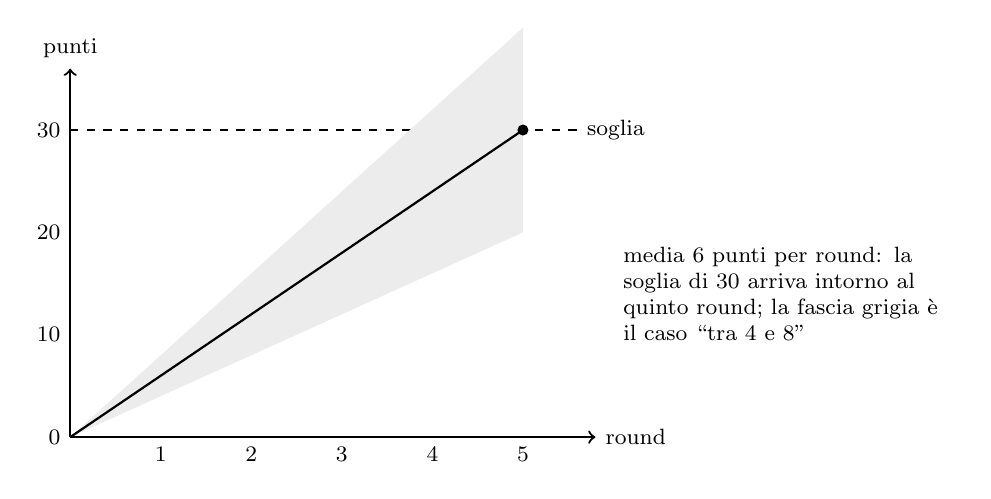
\begin{tikzpicture}[font=\small, x=1.15cm, y=0.13cm]
  \draw[thick, ->] (0,0) -- (5.8,0) node[right, font=\footnotesize] {round};
  \draw[thick, ->] (0,0) -- (0,36) node[above, font=\footnotesize] {punti};
  \foreach \x in {1,...,5} \node[below, font=\footnotesize] at (\x,0) {\x};
  \foreach \y in {0,10,20,30} \node[left, font=\footnotesize] at (0,\y) {\y};
  \draw[dashed] (0,30) -- (5.6,30) node[right, font=\footnotesize] {soglia};
  \fill[gray!15] (0,0) -- (1,4) -- (2,8) -- (3,12) -- (4,16) -- (5,20) -- (5,40) --
    (4,32) -- (3,24) -- (2,16) -- (1,8) -- cycle;
  \draw[thick] (0,0) -- (1,6) -- (2,12) -- (3,18) -- (4,24) -- (5,30);
  \fill (5,30) circle (2pt);
  \node[font=\footnotesize, text width=4.2cm, align=left, anchor=west] at (6.0,14)
    {media 6 punti per round: la soglia di 30 arriva intorno al quinto round; la fascia
    grigia è il caso ``tra 4 e 8''};
\end{tikzpicture}
\caption{Il bilanciamento di durata con una soglia di punti, nell'esempio di Marta su
\emph{Root}: dal numero di round desiderato si ricava quanti punti deve poter fare un
giocatore in un round, e da lì il valore di ogni elemento.}
\label{a14:fig:durata}
\end{figure}

\paragraph{Tagliare i turni iniziali.} Che cosa si può fare per limare la durata? Si possono
\textbf{tagliare i turni iniziali}, che molto spesso presentano \textbf{poche scelte
significative}. Marta non invita a farlo sempre, anzi, ``con molta parsimonia''. Tra addetti
ai lavori si parla di \textbf{bilanciamento di Kramer}\footnote{Così nella trascrizione (``tra
detti e lavori si chiama il bilanciamento di Kramer''). Il riferimento è probabilmente al
designer tedesco Wolfgang Kramer, ma il capitolo non ha trovato una fonte che usi questo nome
per la tecnica.}: si danno \textbf{risorse di partenza} ai giocatori, perché i primi turni non
siano impiegati a raccogliere risorse. Ha delle insidie: rende sicuramente il gioco più
focalizzato e più attento, ma intanto bisogna fare \textbf{un buon bilanciamento delle risorse
iniziali}; e, se le risorse date sono diverse tra i giocatori, bisogna capire se partire con
certe risorse dia \textbf{un vantaggio}. È una cosa da fare \textbf{solo quando è necessaria}.
Alcuni giochi beneficiano di un \textbf{turno iniziale semplice e guidato}, che è anche uno
degli \textbf{strumenti di approcciabilità}: è vero che quei turni si somigliano da una partita
all'altra, ma a volte servono ad agevolare l'ingresso nel gioco. Soprattutto in un gioco
pensato per andare oltre i confini del proprio genere, qualche turno semplice può aiutare le
persone a \textbf{entrare nel flusso}.

\paragraph{Tagliare i turni finali.} Si fa molto spesso negli \textbf{\emph{engine
building}}, i giochi a ``motore economico'', in cui c'è un \emph{feedback} che genera punti
vittoria o risorse, o che comunque avvicina alla condizione di fine partita. Il motore, andando
avanti, diventa sempre più performante; e se da un certo punto cresce in modo
\textbf{lineare o esponenziale}, diventa probabilmente impossibile per gli altri recuperare.
Allora si tagliano i turni finali: ``da questo punto in avanti è chiaro come andrebbe il resto
della partita, non c'è bisogno di giocarla'', per non tediare le altre persone. L'esempio è
\textbf{\emph{Race for the Galaxy}}: la partita finisce quando si esauriscono i
\textbf{gettoni punti} o quando qualcuno ha giocato \textbf{12 carte}. Di solito avviene quando
il motore si è innescato: i turni successivi ripeterebbero quello che si è già visto, perché
le strategie sono ormai impostate.

\paragraph{La durata dentro il turno.} Un'altra parola sulla durata \textbf{intraturno}. Se si
aggiungono tantissime \textbf{microscelte} dentro il turno, la persona si sentirà
\textbf{paralizzata} e spenderà molto tempo. E anche in una situazione normale, con poche
scelte, se per stare dietro a tutte le regole \textbf{vanno via 5 minuti}, quei 5 minuti vanno
\textbf{moltiplicati per il numero di persone e per il numero di round}: la durata di un gioco
cresce molto in fretta. E si stanno ancora omettendo le altre fasi, come quelle di
\textbf{amministrazione} o di \textbf{conteggio dei punti}. Bisogna quindi fare attenzione che
i turni non siano inutilmente lunghi; ma a volte \textbf{un turno lungo può essere molto
soddisfacente}. \emph{Root} dura, a detta di Marta, due ore e mezza, e i suoi turni sono molto
lunghi rispetto ad altri giochi simili; ma senza quei turni e senza quella durata il gioco ne
risentirebbe in termini di esperienza. ``Alla fine conta molto il gioco che stiamo facendo.''

\subsection{La domanda: come si calcola la durata sulla scatola?}

Uno studente chiede: sulle scatole c'è scritto quanto dura un gioco, ma spesso a lui sembra
\textbf{sottodimensionato}. Come viene calcolato? C'è uno standard?

``Lo standard in realtà non c'è'', risponde Marta. Tendenzialmente si dovrebbe indicare
\textbf{la durata media di una partita una volta che si conoscono le regole}. Quindi:
\begin{itemize}
  \item \textbf{non è mai compresa la spiegazione delle regole};
  \item \textbf{non è mai considerata la prima partita}: il valore vale più per chi ha giocato
        tre o quattro volte e conosce il gioco, e non è più al punto di riprendere in mano il
        regolamento.
\end{itemize}
Va da sé che il numero viene \textbf{sbagliato piuttosto spesso}, perché non è facile
stabilirlo. Il metodo migliore, secondo Marta, è prendere \textbf{il tempo medio del gruppo di
\emph{test} che conosce il gioco} e quello di chi fa \textbf{\emph{blind test}}, cioè di persone
alle prime armi, e vedere dove si assesta \textbf{il valore di mezzo}: non tutti giocheranno come
chi ha fatto cento partite, ma neanche ne faranno solo due; l'ideale sarebbe che a un gioco si
facessero \textbf{5--10 partite}. E poi dipende molto dai \textbf{gruppi di gioco}: non c'è un
vincolo su quanto si impiega a fare il proprio turno, e se si è al tavolo con persone che
pensano molto, le durate cresceranno. Si tende comunque a trovare una durata
\textbf{compatibile con il gioco}: un gioco per bambini non può durare due ore, ``ma queste
cose penso le intuite anche voi''.

\paragraph{Approfondimento: corto o lungo.} Schell dedica un intero tipo di bilanciamento
(``corto contro lungo'') alla durata: se il gioco è troppo corto, i giocatori non riescono a
sviluppare ed eseguire strategie significative; se è troppo lungo, si annoiano o lo evitano
per l'impegno di tempo. Le leve principali sono le condizioni di vittoria e di sconfitta. Due
suoi esempi mostrano soluzioni diverse dal taglio di turni: in \emph{Spy Hunter}, per i primi
novanta secondi il giocatore ha auto infinite, perché i principianti non abbiano partite
frustranti di pochi secondi; in \emph{Minotaur}, dopo venti minuti suona una campana e tutti i
sopravvissuti vengono trasportati in una stanza piena di mostri, così la partita finisce in
meno di venticinque minuti e c'è comunque un vincitore, lo stesso principio della zona che si
restringe nei \emph{battle royale}. È convergenza (sezione~\ref{a14:sec:difetti}) imposta per
regola.

% ---------------------------------------------------------------------
\section{Raddoppia o dividi la risorsa}
\label{a14:sec:raddoppia}

Un'altra tecnica ``molto popolare'' è \textbf{raddoppiare o dividere la risorsa}\footnote{Nella
trascrizione ``il raddoppio di vidi la risorsa''.}. A volte è importante capire \textbf{quanto
una risorsa incide sul gioco}, e dove ha senso bilanciarla, se farla crescere o diminuire: non
è sempre semplice capirlo. La tecnica base è: se c'è uno spazio azione dove si ottengono delle
risorse, \textbf{si raddoppia la quantità}, anche se il numero sembra grandissimo,
\textbf{oppure la si divide}. Raddoppiare o dividere è un'\textbf{estremizzazione}, ed
estremizzare una risorsa ne rende subito evidente l'impatto sul gioco: si applica la tecnica e
si vede come reagisce il sistema.

\paragraph{Le dipendenze.} Se la risorsa ha \textbf{tante dipendenze}, il sistema può
``fallire'': la modifica scombina tantissime cose a cascata, e la tecnica diventa praticamente
inutile, perché non restituisce alcun valore certo. Più dipendenze ha, più il rischio è alto.
Per esempio, è \textbf{poco rischioso} applicarla ai \textbf{punti vittoria}: raddoppiare o
dividere i punti di una carta specifica di solito ha poco impatto sul resto delle carte e dei
componenti, perché è \textbf{un valore finale}, con poche dipendenze. Va comunque valutato di
volta in volta.

\paragraph{Quanto deve pesare ogni parte.} Va considerato anche, come questione a sé,
\textbf{quanto valgono le varie parti del gioco}. Se si fa un gioco in cui si costruisce la
propria \textbf{città} sulla propria plancia, e poi ci sono \textbf{obiettivi} e
\textbf{risorse} che danno punti, e il \emph{focus} deve essere la città, allora la città deve
valere \textbf{il 50, 60, anche 70\%} del punteggio totale, riservando il \textbf{10--15\%}
agli altri sistemi che entrano nel conteggio finale. Non è un caso che in
\textbf{\emph{Wingspan}} \textbf{quasi il 50\%} dei punti derivi dalle \textbf{carte uccello} o
dall'uso di determinate abilità, perché sono il \emph{focus} del gioco: difficilmente si fa più
della metà dei punti con le risorse rimaste a fine partita o con le carte obiettivo. È anche una
questione di \textbf{dove mettere il \emph{focus} dell'esperienza}.

\paragraph{Una ricerca progressiva.} La tecnica può essere \textbf{progressiva}: applicando
costantemente il raddoppio o la divisione si arriva a trovare il \textbf{valore medio}. Si
continua a raddoppiare finché la risorsa non diventa \textbf{troppo incisiva}; da lì si torna
a dividere, cioè un po' indietro; e così, stringendo via via il campo, si trova il valore
giusto (figura~\ref{a14:fig:raddoppia}). Anche qui, però, bisogna capire se il valore
``giusto'' è quello che serve a \textbf{veicolare l'intento del \emph{design}}, o se è
semplicemente qualcosa che funziona ma finisce per \textbf{appiattire} il resto delle risorse:
``fare attenzione sempre al solito concetto''.

\begin{figure}[htbp]
\centering
\begin{tikzpicture}[font=\small, x=1.25cm, y=1cm]
  \draw[thick] (0,0) -- (9,0);
  \foreach \x/\l in {0.5/1, 1.5/2, 3.5/4, 7.5/8} {
    \draw (\x,-0.12) -- (\x,0.12);
    \node[below, font=\footnotesize] at (\x,-0.15) {\l};
  }
  \fill[gray!25] (3.5,-0.08) rectangle (7.5,0.08);
  \node[font=\footnotesize] at (5.5,-1.3) {qui sta il valore cercato};
  \draw[-{Stealth[length=2mm]}, thick] (0.5,0.3) to[bend left=40] node[above,
    font=\scriptsize] {$\times 2$} (1.5,0.3);
  \draw[-{Stealth[length=2mm]}, thick] (1.5,0.3) to[bend left=40] node[above,
    font=\scriptsize] {$\times 2$} (3.5,0.3);
  \draw[-{Stealth[length=2mm]}, thick] (3.5,0.3) to[bend left=40] node[above,
    font=\scriptsize] {$\times 2$: troppo!} (7.5,0.3);
  \draw[-{Stealth[length=2mm]}, thick] (7.5,-0.2) to[bend left=40] node[below,
    font=\scriptsize] {a metà strada} (5.5,-0.2);
  \node[font=\footnotesize, text width=4.3cm, align=left, anchor=west] at (9.2,0.2)
    {1: poco incisiva\\ 2, 4: ancora poco\\ 8: troppo incisiva\\ $\Rightarrow$ si torna
    indietro e si stringe tra 4 e 8};
\end{tikzpicture}
\caption{Raddoppia o dividi come ricerca progressiva: si estremizza la risorsa finché il suo
impatto non diventa evidente, poi si torna indietro stringendo l'intervallo. Funziona bene su
valori con poche dipendenze, come i punti vittoria di una carta.}
\label{a14:fig:raddoppia}
\end{figure}

\paragraph{Approfondimento: la regola di Sid Meier.} Schell riporta la stessa tecnica come
``regola del raddoppio e del dimezzamento'': quando si cambia un valore per bilanciare, si
spreca tempo a cambiarlo di poco; conviene raddoppiarlo o dimezzarlo nella direzione in cui
deve andare, e poi, se si è esagerato, provare a metà strada. L'esempio è un razzo che fa 100
punti di danno: se sembrano troppi, non si scende a 90 o 80, ma a 50. La regola è spesso
attribuita a Brian Reynolds, che però, interpellato da Schell, ne dà il merito a \textbf{Sid
Meier}: lo prese da parte, all'inizio degli anni Novanta, mentre lavoravano a
\emph{Colonization}, dopo averlo visto cambiare ripetutamente un valore del 10\%. Il punto,
dice Reynolds, è cambiare qualcosa in modo da \emph{sentire} subito la differenza, invece di
perdersi a chiedersi se si è avuto un effetto, o peggio vederne uno che non c'è, magari per
una serie sfortunata di numeri casuali.

% ---------------------------------------------------------------------
\section{Due problemi, una soluzione}
\label{a14:sec:dueproblemi}

Un'altra tecnica molto usata, soprattutto \textbf{all'inizio dello sviluppo}: \textbf{due
problemi, una soluzione}. Quando si trova un problema, \textbf{non lo si risolve subito}: se ne
cerca \textbf{almeno un altro}, e si applica \textbf{una soluzione a entrambi}, cioè una sola
modifica che li risolva tutti e due. Questo aiuta a \textbf{far convergere il lavoro}, verso
una riduzione del numero di problemi: magari la soluzione ne fa emergere un altro, ma
generalmente \textbf{non ne fa emergere altri due}, e così si progredisce.

È utile all'inizio. Applicata \textbf{verso la fine}, ci si accorge che intanto è \textbf{poco
efficace}, e soprattutto che la soluzione trovata \textbf{impatta molto più forte} su tutti gli
altri sistemi. Il consiglio è di usarla principalmente all'inizio, e di fare attenzione
\textbf{all'impatto di ciascuna leva}: risolvendo due problemi con una nuova soluzione si
modificano leve che a loro volta possono creare problemi. Purtroppo questo si risolve solo in
due modi: con \textbf{l'esperienza}, cioè sapendo più o meno che cosa succede quando si
applicano certe soluzioni, e con i \textbf{\emph{test}}, perché a volte non c'è modo di
risolvere i problemi se non empiricamente.

% ---------------------------------------------------------------------
\section{Gli elementi ricorrenti del bilanciamento}
\label{a14:sec:elementi}

Seguono ``vari elementi'' che ricorrono quando si parla di bilanciamento e di sviluppo, e per
cui Marta non ha trovato ``un modo coerente di metterli'': in questa slide ha cercato di
trasmettere ``quelle cose che si apprendono un po' per esperienza''. La
tabella~\ref{a14:tab:elementi}, alla fine della sezione, li riassume.

\subsection{Le progressioni di punteggio}

Ci sono \textbf{progressioni note} per i punteggi. Una classica è \textbf{1, 3, 6, 10, 15}: tra
un numero e l'altro l'incremento cresce di uno (+2, +3, +4, +5). Serve, per esempio, in una
\textbf{collezione di set}, a rendere la collezione \textbf{sempre più premiante} man mano che
cresce. Una progressione ancora più forte è quella \textbf{quadratica}: con 5 pezzi di una
risorsa si fanno \textbf{25 punti}; cresce molto più rapidamente dell'altra, e quindi si dà
\textbf{ancora più importanza} a quella risorsa. Oppure ci può essere una progressione
\textbf{penalizzante}: dà punti fino a un certo punto, per esempio 1, 3, 6, e poi
\textbf{scende}, 5, 4; dice che quella risorsa la si vuole, \textbf{``ma non troppo''}
(figura~\ref{a14:fig:progressioni}).

Sono elementi che tornano comodi quando si ha una collezione di set e si vuole creare una certa
esperienza in linea con il \emph{design}. Molto spesso la prima cosa che si fa è prendere una
di queste progressioni ``classiche'', applicarla e vedere come reagisce il gioco; ``in rari casi
vengono cambiate''.

\begin{figure}[htbp]
\centering
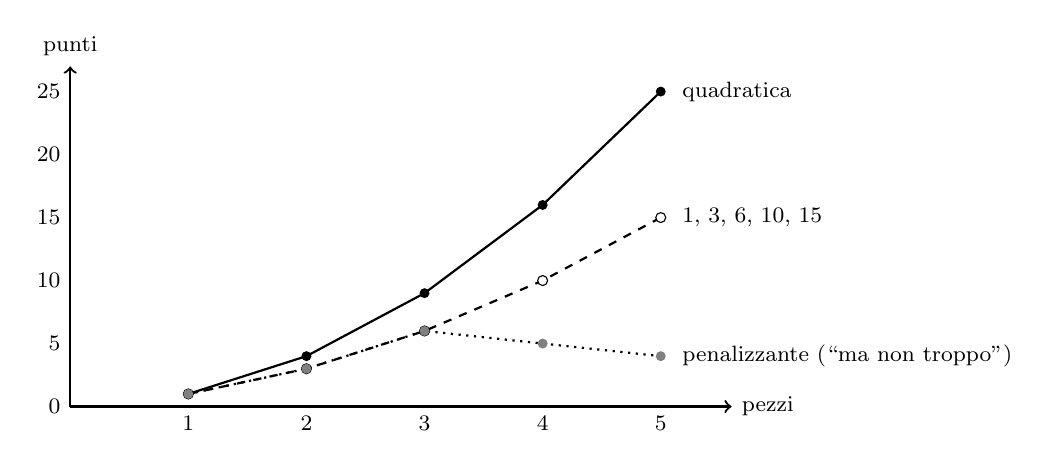
\begin{tikzpicture}[font=\small, x=1.5cm, y=0.16cm]
  \draw[thick, ->] (0,0) -- (5.6,0) node[right, font=\footnotesize] {pezzi};
  \draw[thick, ->] (0,0) -- (0,27) node[above, font=\footnotesize] {punti};
  \foreach \x in {1,...,5} \node[below, font=\footnotesize] at (\x,0) {\x};
  \foreach \y in {0,5,10,15,20,25} \node[left, font=\footnotesize] at (0,\y) {\y};
  % quadratica
  \draw[thick] (1,1) -- (2,4) -- (3,9) -- (4,16) -- (5,25);
  \foreach \x/\y in {1/1,2/4,3/9,4/16,5/25} \fill (\x,\y) circle (1.8pt);
  \node[font=\footnotesize, anchor=west] at (5.1,25) {quadratica};
  % triangolare
  \draw[thick, dashed] (1,1) -- (2,3) -- (3,6) -- (4,10) -- (5,15);
  \foreach \x/\y in {1/1,2/3,3/6,4/10,5/15} \fill[white, draw=black] (\x,\y) circle (1.8pt);
  \node[font=\footnotesize, anchor=west] at (5.1,15) {1, 3, 6, 10, 15};
  % penalizzante
  \draw[thick, dotted] (1,1) -- (2,3) -- (3,6) -- (4,5) -- (5,4);
  \foreach \x/\y in {1/1,2/3,3/6,4/5,5/4} \fill[gray] (\x,\y) circle (1.8pt);
  \node[font=\footnotesize, anchor=west] at (5.1,4) {penalizzante (``ma non troppo'')};
\end{tikzpicture}
\caption{Le tre progressioni di punteggio di cui parla Marta. Più ripida è la curva, più il
gioco spinge a concentrarsi su quella collezione; una curva che scende dopo un massimo dice
che la risorsa serve, ma non in eccesso.}
\label{a14:fig:progressioni}
\end{figure}

\subsection{Mettere in relazione le risorse: moltiplicazioni e set}

\paragraph{La moltiplicazione.} Si possono \textbf{mettere in relazione due risorse}, per
esempio con una \textbf{moltiplicazione}: si ottengono punti pari a \textbf{risorsa A per risorsa
B}. L'intento di sviluppo che questo veicola è che si vogliono \textbf{possibilmente tante A
quante B}, e non tante dell'una e poche dell'altra: per come funziona la moltiplicazione, a
parità di pezzi totali si ottiene di più se i due numeri sono uguali che se uno è molto alto e
l'altro molto basso (con 6 pezzi, $3 \times 3 = 9$, mentre $5 \times 1 = 5$). È una cosa che si
adotta quando si vede che c'è \textbf{troppa concentrazione su una delle due risorse}, magari
perché risulta più premiante: la moltiplicazione le \textbf{ribilancia}, in modo che abbiano lo
stesso interesse.

\paragraph{Il set.} Lo stesso vale per più di due risorse, tre o quattro, quando si vuole che
nel gioco \textbf{siano tutte importanti} e non vengano trascurate: allora si premia
\textbf{il set}. Per ogni set completo, cioè almeno una di ciascuna risorsa, si dà un certo
punteggio.

\paragraph{Punteggio verticale e orizzontale.} Marta non ricorda il termine inglese di
partenza (``mi sfugge il termine'') e li chiama \textbf{punteggio verticale} e
\textbf{punteggio orizzontale}. Il \textbf{verticale} è quello classico: questa risorsa dà
tanto, quest'altra tanto, per quello che ho ottenuto nel gioco. L'\textbf{orizzontale} prende
\textbf{l'altro asse}, e analizza \textbf{quante risorse diverse} ho ottenuto: è il caso, molto
spesso, del calcolo dei set di risorse.

``Anche queste sono tutte cose che trovate standard.'' Ed è anche per questo, come diceva la
volta precedente, che è importante \textbf{giocare tanti giochi}, conoscere tanto, avere
curiosità, esplorare anche giochi \textbf{fuori dalla propria \emph{comfort zone}} e
guardarli con occhio critico: ci si accorge che molte di queste cose sono riusate in
tantissimi giochi.

\subsection{L'esclusività delle risorse}

Si torna all'esempio di \emph{Splendor}: c'è un motivo per cui lì le risorse sono
\textbf{esclusive}, cioè i gettoni sono \textbf{in numero prefissato}. ``Mi sembra che sono
10, ora non sono sicurissima''\footnote{Nel gioco i gettoni gemma sono 7 per colore, più 5
gettoni oro jolly, e se ne usano meno con due o tre giocatori. Il numero esatto non cambia il
ragionamento di Marta.}, per ogni risorsa, e le persone ne possono prendere \textbf{tre a turno}
con la propria azione. Essendo esclusive, il gioco si basa anche sulla \textbf{scarsità}: è una
strategia lecita \textbf{prendere delle risorse per toglierle} agli altri e fare in modo che
non ci siano per le altre persone al tavolo. E l'effetto si propaga: se c'è una carta che
interessa a più giocatori, togliendo la risorsa dal tavolo la carta diventa \textbf{esclusiva a
sua volta}, perché nessun altro la può completare. Poi la cosa si manifesta come un aspetto di
\textbf{\emph{timing}}: diventa importante \textbf{quando} restituire quelle risorse.

\paragraph{Da limite a opportunità.} Marta lo dice perché molto spesso l'esclusività delle
risorse è nata come \textbf{limite}, per via del \textbf{numero di componenti}: essendo un
prodotto fisico, come visto parlando dei limiti della componentistica, è complicato mettere
tante cose in una scatola. Ma, come tutti i limiti, a un certo punto è diventata
un'\textbf{opportunità} di \emph{design} e di sviluppo: quando ci si accorge che c'è
\textbf{poca interazione tra i giocatori}, introdurre l'esclusività delle risorse a volte fa
esattamente quello che serve per \textbf{generare interazione}. Lo stesso vale per gli
\textbf{incentivi}, sia nel restituire queste risorse sia nel prenderle, nel caso la risorsa
sia esclusiva ma i giocatori non la prendano in considerazione.

\subsection{La crescita tra i round}

Un altro aspetto importante è la \textbf{crescita tra round}. In molti giochi è importante che
tra un round e l'altro \textbf{ci sia una differenza}: se in tutti i round si ha accesso alle
stesse identiche risorse, la stessa situazione sulla plancia, le stesse possibilità, il gioco
risulta \textbf{statico}. La crescita fa percepire \textbf{la progressione} a chi gioca. A volte
viene tralasciata, ma si può fare in modo abbastanza semplice: se c'è una \textbf{rendita}, la
rendita cresce; oppure, man mano che si piazzano cose sul tabellone, si \textbf{sbloccano} cose
sulla propria plancia che danno più possibilità andando avanti. È un elemento che nello
sviluppo viene esaminato molto spesso, perché magari il gioco funziona, ma ha \textbf{una
crescita piatta}, e bisogna lavorare per farla aumentare.

\subsection{Il controllo dell'alea e del caos}

Altro elemento frequente: il \textbf{controllo dell'alea o del caos}. Il gioco può presentare
sia alea sia caos, ma in modo \textbf{estremizzato}, e allora bisogna trovare strumenti per
regolarli. L'esempio più classico: \textbf{lancio un dado e spendo una risorsa per fare il
\emph{re-roll}}. Molti giochi con questa meccanica non avevano di base il \emph{re-roll}: è
stato aggiunto \textbf{in fase di sviluppo}, perché si è visto che il lancio di dado senza
possibilità di rilancio è un'esperienza \textbf{frustrante} per la maggior parte di chi gioca.
C'è poi l'esempio pratico di \textbf{\emph{Magical Athlete}}, che ha ``abbattuto un po' questa
concezione'': oggi ci sono giochi che accettano ``un po' più di buon grado'' anche il lancio
del dado senza controllo. Ma in fase di sviluppo questo resta uno degli elementi su cui si va a
incidere. Un altro esempio: tessere pescate \textbf{da un sacchetto}, con la possibilità di
\textbf{pescarne più di una}, o di \textbf{rimettere} quella pescata e pescarne un'altra.

\subsection{Le probabilità}

È utile avere \textbf{una base di probabilità}. L'esempio più classico è il dado, e sapere come
usare i dadi in un gioco ``può fare la differenza''.

\paragraph{Lineare.} Un dado da 1 a 6 ha una probabilità cosiddetta \textbf{lineare}
(uniforme): ogni faccia ha la stessa probabilità di uscire.

\paragraph{A campana.} Con \textbf{due dadi} la probabilità segue una \textbf{curva a campana}:
il risultato medio è più probabile dei risultati agli estremi. ``Penso che questo lo sappiate'':
con due dadi è molto più probabile fare \textbf{7} che fare 2 o 12. È una particolarità che può
\textbf{informare le decisioni}. Si immagini un \textbf{gioco di percorso} in cui si lancia un
solo dado: si dà la stessa probabilità a tutte le facce, e mediamente ci si muove di
\textbf{3,5}, il valore medio di un dado. Con due dadi, invece, uscirà più spesso il 7: è un
sistema ``più morbido'', perché i risultati estremi sono più rari. Con un dado solo, il 6 può
uscire tanto quanto il 3 o il 4, e solo su molti lanci la media si riporta a 3,5. Questo aiuta
a capire che cosa serve in funzione del gioco (figura~\ref{a14:fig:dadi}).

\paragraph{Calante.} La probabilità può anche essere \textbf{calante}. Si immagini di poter
scegliere quante risorse ottenere, \textbf{da una a cinque}, ma per ogni risorsa voluta bisogna
\textbf{lanciare una moneta}. Se se ne prende una, si lancia una moneta: con testa la si tiene,
con croce no. Se se ne vogliono cinque, si lanciano cinque monete, ma \textbf{basta una sola
croce per non tenerne nessuna}. La probabilità \textbf{cala} al crescere delle risorse che si
vogliono ottenere. Si usa anche questo: per esempio, in un gioco di percorso, ``posso muovermi
di quanto mi pare, ma poi lancio il dado'', e se il risultato è inferiore allo spostamento
dichiarato devo tornare indietro, o non mi muovo affatto.

Sono piccoli meccanismi che influenzano e guidano le scelte, e che aiutano a regolare lo
sviluppo: magari in fase di \emph{design} si è detto ``mi interessa che sia un gioco di
percorso, mi basta lanciare un dado da 6 e andare dove vado''; ma in sviluppo si vuole che la
decisione sia \textbf{più controllata}, e si possono inserire strutture come il
\textbf{cambiare la probabilità} di quel meccanismo.

\begin{figure}[htbp]
\centering
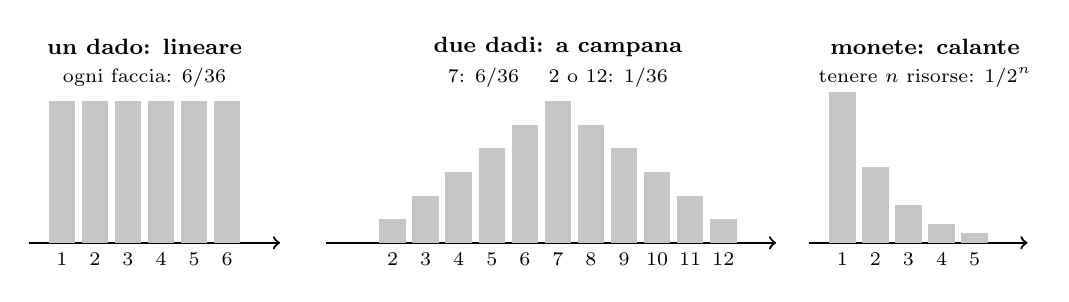
\begin{tikzpicture}[font=\small, x=0.42cm, y=0.30cm]
  % un dado
  \node[font=\footnotesize\bfseries] at (3.5,8.3) {un dado: lineare};
  \draw[thick, ->] (0,0) -- (7.6,0);
  \foreach \v in {1,...,6} {
    \fill[gray!45] (\v-0.4,0) rectangle (\v+0.4,6);
    \node[below, font=\scriptsize] at (\v,0) {\v};
  }
  \node[font=\scriptsize] at (3.5,7.0) {ogni faccia: 6/36};
  % due dadi
  \begin{scope}[shift={(9,0)}]
    \node[font=\footnotesize\bfseries] at (7,8.3) {due dadi: a campana};
    \draw[thick, ->] (0,0) -- (13.6,0);
    \foreach \v/\h in {2/1,3/2,4/3,5/4,6/5,7/6,8/5,9/4,10/3,11/2,12/1} {
      \fill[gray!45] (\v-0.4,0) rectangle (\v+0.4,\h);
      \node[below, font=\scriptsize] at (\v,0) {\v};
    }
    \node[font=\scriptsize] at (7,7.0) {7: 6/36 \quad 2 o 12: 1/36};
  \end{scope}
  % monete
  \begin{scope}[shift={(23.6,0)}]
    \node[font=\footnotesize\bfseries, align=center] at (3.5,8.3) {monete: calante};
    \draw[thick, ->] (0,0) -- (6.6,0);
    \foreach \v/\h in {1/6.4,2/3.2,3/1.6,4/0.8,5/0.4} {
      \fill[gray!45] (\v-0.4,0) rectangle (\v+0.4,\h);
      \node[below, font=\scriptsize] at (\v,0) {\v};
    }
    \node[font=\scriptsize, align=center] at (3.5,7.0) {tenere $n$ risorse: $1/2^n$};
  \end{scope}
\end{tikzpicture}
\caption{Le tre forme di probabilità dell'esempio di Marta: il dado singolo (ogni faccia
ugualmente probabile, media 3,5), due dadi (il 7 è sei volte più probabile del 2 o del 12) e la
probabilità calante delle monete (per tenere $n$ risorse servono $n$ teste di fila: 50\%,
25\%, 12,5\%\ldots). Le barre sono in scala all'interno di ciascun grafico.}
\label{a14:fig:dadi}
\end{figure}

\begin{table}[htbp]
\centering
\small
\begin{tabular}{@{}p{3.2cm}p{5.2cm}p{5.0cm}@{}}
\toprule
\textbf{Tecnica o elemento} & \textbf{Che cosa fa} & \textbf{Attenzione a} \\
\midrule
Budget di complessità & ciò che si toglie libera complessità, da eliminare o reinvestire
  nel \emph{focus} & nel dubbio, meglio accessibile \\
\addlinespace
Alto e basso rischio & crea una scelta sensibile con due macro-strategie comunicanti & la
  ricompensa deve valere il rischio \\
\addlinespace
Ancoraggio & tutto è rapportato a un valore ancora (\emph{Stone Age}: un puntino = un punto)
  & risorse interdipendenti, turni extra, \emph{draft} \\
\addlinespace
Durata & round o soglie fissate $\Rightarrow$ punti per round $\Rightarrow$ valore dei
  pezzi; tagliare turni iniziali o finali & la durata intraturno si moltiplica per persone
  e round \\
\addlinespace
Raddoppia o dividi & estremizza per vedere l'impatto, poi stringe & le dipendenze; il
  valore ``giusto'' può appiattire \\
\addlinespace
Due problemi, una soluzione & fa convergere il lavoro & solo all'inizio dello sviluppo \\
\addlinespace
Progressioni & 1-3-6-10-15, quadratica, penalizzante & che cosa si vuole premiare \\
\addlinespace
$A \times B$ e set & spingono a bilanciare le risorse tra loro & punteggio verticale contro
  orizzontale \\
\addlinespace
Esclusività & scarsità, interazione, \emph{timing} & nata come limite di componenti \\
\addlinespace
Crescita tra round & progressione percepita (rendite, sblocchi) & la crescita piatta \\
\addlinespace
Controllo dell'alea & \emph{re-roll}, più pescate, rimettere nel sacchetto & non sempre serve
  (\emph{Magical Athlete}) \\
\addlinespace
Probabilità & lineare, a campana, calante & scegliere la forma che serve all'esperienza \\
\bottomrule
\end{tabular}
\caption{Gli strumenti di bilanciamento presentati nella lezione, nell'ordine in cui li
presenta Marta.}
\label{a14:tab:elementi}
\end{table}

\paragraph{Approfondimento: la probabilità per chi progetta.} Schell dedica un capitolo alla
probabilità con dieci ``regole'', e una delle sue osservazioni conferma il consiglio di Marta
di testare invece di calcolare: il \emph{metodo Monte Carlo}, cioè ripetere la prova molte volte
e contare i risultati, ``a volte dà risultati più utili della probabilità teorica, perché è una
misura della cosa reale''. La sua ultima regola, scherzosa, è la più pratica: quando un calcolo
si fa difficile, cercare qualcuno che si consideri ``un mago della matematica'', che ne sarà
entusiasta. Brathwaite e Schreiber, in \emph{Challenges for Game Designers}, dedicano invece un
intero capitolo all'equilibrio tra caso e abilità, il tema del controllo dell'alea.

% ---------------------------------------------------------------------
\section{Smussare la stella}
\label{a14:sec:stella}

``Vediamo, ok. Forse devo correre un po', allora.'' \textbf{Non è detto che chi crea il gioco
abbia chiaro il \emph{design}.} Per spiegarlo Marta usa un modo di dire: un gioco è
\textbf{una stella}, e lo sviluppo \textbf{smussa gli angoli}, perché le punte non blocchino
l'ingresso in un ipotetico buco (``non so come dirlo meglio''). Le punte rappresentano le
\textbf{qualità e le particolarità del \emph{design}}. Come detto la volta prima, il
\emph{design} è anche \textbf{personale} e dovrebbe sfuggire un po' alle logiche di mercato; e
così anche lo sviluppo. Oggi tenere alcune punte è diventato più importante che in passato;
tuttavia si smussa, perché \textbf{più punte ha la stella, meno è digeribile per un pubblico
ampio}: le persone hanno bisogno di un po' di \textbf{familiarità} e di un po' di
\textbf{novità}, non accettano una cosa totalmente innovativa, ma neanche ne vogliono una
estremamente familiare. È un gioco di \textbf{trovare il punto giusto}.

\paragraph{Chi ha creato il gioco può non vedere l'intento.} In questo, a volte, anche chi ha
creato il gioco ha poco chiaro l'intento del \emph{design}, nonostante il gioco lo manifesti:
viene fuori giocandolo. Lo sviluppo deve però evitare di \textbf{finire sui \emph{bias}
personali}: se si ha un genere preferito, bisogna fare attenzione a non mettere la propria
preferenza in tutti i giochi. Se si fa un gioco per bambini, è inutile metterci le dinamiche di
un \textbf{motore economico}: ``non funziona'', o quanto meno sarà molto complicato far capire a
un bambino come funziona economicamente un motore di gioco. ``So che sembra una banalità'', ma è
una tendenza in cui si cade con estrema facilità, anche in casi che sembrano estremi.

\paragraph{Il GCD come bussola.} Il \textbf{\emph{Game Concept Document}} dà il \emph{focus} per
restare sul progetto: averlo sempre a portata di mano aiuta a ricordare che cosa si sta
facendo, come lo si sta facendo, e \textbf{che cosa si può davvero smussare} senza intaccare
uno dei \textbf{pilastri}, cosa che comprometterebbe davvero il \emph{design}. Resta il fatto che
\textbf{se una cosa non è fondamentale all'esperienza, può essere tolta}.

\paragraph{Ma attenzione a che cosa è ``fondamentale''.} La valutazione personale porta sempre
il rischio di sbagliarsi. Una cosa che \textbf{sembra} non fondamentale, come i \textbf{testi di
ambientazione} (\emph{flavor text}) su alcune carte, solo perché non entrano in gioco in modo
meccanico, a volte viene considerata non incisiva. Ma se \textbf{\emph{Wingspan}} non avesse i
testini che raccontano i comportamenti degli uccelli e tutto il resto, probabilmente non avrebbe
la stessa potenza, la stessa capacità di fare leva su tantissime persone che ha avuto nella
pratica. Alcune cose non sembrano fondamentali, ``ma fanno la differenza''.

\paragraph{Approfondimento: l'eleganza e il dettaglio.} Schell elenca tra i dodici tipi di
bilanciamento anche ``semplice contro complesso'' e ``dettaglio contro immaginazione'', e
propone una \emph{lente dell'eleganza}: un sistema elegante fa molto con pochi elementi. Ma per
lui l'eleganza non è il taglio indiscriminato: i dettagli che \emph{nutrono} l'immaginazione,
e che l'immaginazione può riusare più e più volte, vanno tenuti. I testi di \emph{Wingspan} sono
esattamente questo tipo di dettaglio.

% ---------------------------------------------------------------------
\section{I ``difetti'' dei giochi da tavolo}
\label{a14:sec:difetti}

``Ok, vediamo alcuni dei difetti cosiddetti dei giochi da tavolo.'' Le virgolette sono volute:
molte di queste cose vengono elencate come difetti, \textbf{ma non lo sono}. Lo sono se sono
\textbf{una dinamica che va contro l'esperienza attesa}: ``tendenzialmente sì, se va contro
l'esperienza attesa, di fatto lo possiamo chiamare difetto''. Ma \textbf{non esistono meccaniche
che siano difetti a priori}: vanno viste in funzione del gioco. Molto spesso le persone
confondono le meccaniche che generano \textbf{stati d'animo negativi} (la
\textbf{frustrazione}, a volte la \textbf{noia}) con difetti del gioco. Non è sempre così.
\textbf{Attenzione ai \emph{feedback}}, quindi: molto spesso vi elencheranno queste cose come
difetti, e non è detto che lo siano. Una slide lo riassume: bisogna distinguere
\textbf{l'intento del \emph{design}} dalle \textbf{dinamiche incontrollate}. Il ``difetto'' era
un intento del \emph{design}, oppure è lì perché è un \textbf{aspetto vestigiale del genere}, e
genera dinamiche che neanche il designer sa controllare? La tabella~\ref{a14:tab:difetti} li
riassume.

\paragraph{L'eliminazione dei giocatori: \emph{Bang!}.} La \textbf{\emph{player elimination}}
viene prima perché probabilmente la conoscono tutti, per via di \textbf{\emph{Bang!}}. Tantissime
persone si lamentano di \emph{Bang!} perché c'è l'eliminazione dei giocatori, ma poche si
rendono conto che \textbf{\emph{Bang!} senza eliminazione non funzionerebbe}: sarebbe un gioco
poco efficace. L'eliminazione garantisce che \textbf{tutta la partita sia giocata in tensione};
che non si possano \textbf{scaricare le risorse} liberamente senza pensarci, perché poi si
giocherebbe tutta la partita senza risorse; e fa tutta la differenza sulle
\textbf{ritorsioni}: in certi casi ``posso permettermi di finire le risorse perché so che non
subirò ritorsioni'', cosa che senza eliminazione non sarebbe possibile. La narrativa sottesa di
\emph{Bang!}, e il motivo per cui continua a piacere a tantissime persone, è legata anche
all'eliminazione: è un gioco sul \textbf{Far West}, in un certo senso spietato, che vuole
trasmettere una narrativa con \textbf{\emph{high stakes}}, una posta in gioco
altissima\footnote{Marta dice ``delle \emph{high stakes}, delle alte\ldots{} non mi torna il
termine italiano, perdonatemi''.}. Ci sono però giochi in cui l'eliminazione è \textbf{poco
giustificata}: in un gioco in cui si coopera per salvare il pianeta, ha poco senso eliminare
un giocatore a caso, ``adesso faccio per dire; poi magari trovate la chiave di lettura per cui
ha senso''.

\paragraph{\emph{Runaway leader} e \emph{bash the leader}: \emph{Root}.} Anche queste sono
spesso viste come negative. Il \textbf{\emph{runaway leader}} è quando un giocatore prende un
distacco tale che diventa difficile recuperarlo. La dinamica contrapposta è il \textbf{\emph{bash
the leader}}\footnote{Nella trascrizione ``Base the Leader'' e ``best dei leader''.}: le persone
individuano chi potrebbe ``correre via'' e vincere, e lo \textbf{bastonano}, letteralmente;
tutti se la prendono con la stessa persona, quella in testa. Entrambe possono essere utili in
giochi che rappresentano \textbf{dinamiche di potere}. \emph{Root}, che rappresenta proprio le
dinamiche di potere tra fazioni diverse, ha fatto del \emph{bash the leader} una delle sue
caratteristiche peculiari: il designer l'ha voluta mettere dentro con l'obiettivo di far
ruotare il gioco attorno a questa cosa. Non è una dinamica non voluta: è
\textbf{desiderata}, e il gioco dà gli strumenti sia per metterla in pratica sia per evitare che
diventi incontrastabile.

\paragraph{I \emph{feedback loop}.} Sono quando le risorse o i meccanismi di gioco
\textbf{informano la decisione successiva}. Un \emph{feedback loop} \textbf{positivo}: spendo
risorse e ottengo punti vittoria, e magari un'altra risorsa, che posso usare per ottenere altri
punti e altre risorse: ``capite che cresce all'infinito''. Un \emph{feedback loop}
\textbf{negativo}: eseguire qualcosa non dà qualcosa che rinforza il ciclo, e quindi rifarlo non
è premiante, e questo smorza le fasi successive. Sono dinamiche da tenere d'occhio, perché
possono compromettere l'intento.

\paragraph{Il \emph{kingmaking}.} ``Il \emph{kingmaking} è un'altra\ldots{} vabbè'': Marta non si
dilunga, ``se avete qualche curiosità''\footnote{Il \emph{kingmaking} è la situazione in cui
un giocatore che non può più vincere decide, con le sue mosse, chi tra gli altri vincerà.}.

\paragraph{Divergenza e convergenza.} Le trova ``sempre interessanti''. Molto spesso i giochi
\textbf{non convergono}, cioè non arrivano a una fine: il \emph{design} magari è bello, ma chi
l'ha creato \textbf{non ha pensato a come finisce}, e il gioco può \textbf{stallare}, non
concludersi mai. Bisogna sapere come farlo convergere, e ci sono meccanismi per farlo. Se la
fine del gioco è legata alla \textbf{fine del mazzo}, in un gioco in cui le carte vengono
\textbf{rimesse nel mazzo}, c'è \textbf{divergenza}: il gioco potrebbe non finire mai, perché il
mazzo non finisce mai. Se invece le carte pescate \textbf{non vengono reinserite} in nessun modo
e ogni turno se ne devono pescare \textbf{due}, si sa che \textbf{entro $n/2$ turni la partita
sarà finita}, con $n$ carte nel mazzo (figura~\ref{a14:fig:convergenza}). ``Vedete, questi
valori un po' così, perché è un po' diverso il valore vero; tuttavia fate finta che ora vada
bene''\footnote{La precisazione di Marta è giusta: se a pescare sono più giocatori, o se ci sono
altri modi di consumare il mazzo, il conto cambia. Il principio, cioè che una risorsa che si
consuma senza tornare indietro garantisce la fine, resta.}.

\begin{figure}[htbp]
\centering
\begin{tikzpicture}[
  font=\small,
  a14b/.style={draw, thick, rounded corners=3pt, text width=2.0cm, align=center,
               minimum height=0.9cm, fill=white},
  a14arr/.style={-{Stealth[length=2.5mm]}, thick}
]
  \node[font=\footnotesize\bfseries] at (2.0,1.6) {divergente};
  \node[a14b] (m1) at (0,0) {mazzo};
  \node[a14b] (g1) at (4,0) {gioco};
  \draw[a14arr] (m1.north east) to[bend left=25] node[above, font=\footnotesize] {pesca}
    (g1.north west);
  \draw[a14arr] (g1.south west) to[bend left=25] node[below, font=\footnotesize]
    {rimetti nel mazzo} (m1.south east);
  \node[font=\footnotesize, text width=4.6cm, align=center] at (2.0,-1.75) {il mazzo non
    finisce mai: la partita può stallare};
  \node[font=\footnotesize\bfseries] at (9.0,1.6) {convergente};
  \node[a14b] (m2) at (7,0) {mazzo da $n$ carte};
  \node[a14b] (g2) at (11,0) {scarti};
  \draw[a14arr] (m2) -- node[above, font=\footnotesize] {2 a turno} (g2);
  \node[font=\footnotesize, text width=4.6cm, align=center] at (9.0,-1.75) {niente torna
    indietro: entro circa $n/2$ turni la partita finisce};
\end{tikzpicture}
\caption{Divergenza e convergenza nell'esempio di Marta: legare la fine della partita alla fine
di un mazzo funziona solo se il mazzo si consuma davvero.}
\label{a14:fig:convergenza}
\end{figure}

\paragraph{L'ordine di turno.} Infine, attenzione all'\textbf{ordine di turno}: come sono
disposti i giocatori può \textbf{influenzare la partita di chi segue}, e il \textbf{primo
giocatore} potrebbe avere dei vantaggi. Anche \textbf{come sono distribuite le risorse
iniziali} tra i giocatori va guardato con attenzione. L'esempio classico è fare una serie di
\emph{test} attenti proprio a questo: se faccio iniziare sempre la stessa persona e questa
vince sistematicamente, da qualche parte c'è un problema. Questo è uno di quei casi che
``raramente può non essere un difetto: tendenzialmente lo è''. Ma anche qui c'è un'eccezione:
in un gioco che vuole mostrare \textbf{meccanismi di potere diversi}, il primo giocatore può
essere avvantaggiato di proposito. Marta pensa a \textbf{\emph{Il Grande Dalmuti}}, in cui il
Grande Dalmuti, che comincia a giocare, è avvantaggiato: ma quello è un gioco che vuole proprio
far percepire \textbf{la differenza di potere} tra i giocatori al tavolo\footnote{\emph{Il Grande
Dalmuti} è anch'esso di Richard Garfield (1995).}.

\begin{table}[htbp]
\centering
\small
\begin{tabular}{@{}p{3.0cm}p{4.8cm}p{5.6cm}@{}}
\toprule
\textbf{``Difetto''} & \textbf{Che cos'è} & \textbf{Quando è voluto (esempio di Marta)} \\
\midrule
\emph{Player elimination} & un giocatore esce dalla partita & \emph{Bang!}: tensione, niente
  risorse sprecate, ritorsioni, narrativa del Far West \\
\addlinespace
\emph{Runaway leader} & un distacco irrecuperabile & in giochi sulle dinamiche di potere \\
\addlinespace
\emph{Bash the leader} & tutti contro chi è in testa & \emph{Root}: il gioco ruota attorno a
  questo, e dà strumenti per farlo e per evitarlo \\
\addlinespace
\emph{Feedback loop} & positivo: cresce all'infinito; negativo: rifare non premia & da tenere
  d'occhio rispetto all'intento \\
\addlinespace
\emph{Kingmaking} & chi non può vincere decide chi vince & (non approfondito) \\
\addlinespace
Divergenza & il gioco non converge, stalla & mai: va fatto convergere \\
\addlinespace
Ordine di turno & chi inizia vince sistematicamente & raramente: \emph{Il Grande Dalmuti}, che
  vuole far sentire la differenza di potere \\
\bottomrule
\end{tabular}
\caption{I ``difetti'' dei giochi da tavolo: dinamiche che diventano difetti solo se vanno
contro l'esperienza attesa. La domanda è sempre se siano intento del \emph{design} o dinamiche
incontrollate, magari vestigia del genere.}
\label{a14:tab:difetti}
\end{table}

\paragraph{Approfondimento: \emph{feedback} positivo e durata.} Il caso del \emph{runaway
leader} è lo stesso problema dei turni finali degli \emph{engine building}: un ciclo di
\emph{feedback} positivo che rende la partita decisa prima della fine. Le soluzioni viste in
lezione sono tre e si possono combinare: chiudere la partita quando il motore si è innescato
(\emph{Race for the Galaxy}), dare agli altri giocatori strumenti per frenare chi è in testa
(\emph{Root}), o introdurre cicli negativi che smorzino il vantaggio. Schell nota, a proposito
di \emph{Monopoly}, quanto la durata dipenda da queste dinamiche: giocato con le regole
ufficiali dura circa novanta minuti, ma molti gruppi aggiungono \emph{house rules} (premi in
denaro, meno obblighi di acquisto) che rallentano la convergenza e lo portano a tre ore o più.

% ---------------------------------------------------------------------
\section{La domanda sulle sinergie: bilanciare per tentativi}
\label{a14:sec:sinergie}

Le slide successive contengono una serie di esempi tratti da giochi commerciali; ma
``visto che ci avviamo a conclusione'', Marta preferisce dare la precedenza alle domande.

Ne arriva una da uno studente che, si scusa, sta \textbf{guidando} (``scusate, sono in
macchina''). Gli strumenti visti gli sono sembrati molto utili, ma c'è una cosa che farebbe
ancora fatica a fare. Si immagini un \textbf{\emph{engine building}} in cui le singole carte
hanno un certo valore, ma \textbf{il loro valore combinato è più alto della somma dei valori
singoli}: tutti i casi in cui una strategia vale più delle componenti che la formano.
\textbf{Come si bilanciano?}

``Mi sembra un caso molto specifico'', risponde Marta: ``chiaramente non ho una bacchetta
magica''. Andrebbe visto nel dettaglio, capendo le dipendenze. ``Così a naso'': se le carte da
sole valgono poco e insieme valgono di più, si sta \textbf{premiando il set di quelle carte}.
Bisogna capire \textbf{quante sinergie} hanno queste carte, \textbf{con quante carte} si
sinergizzano, quali sono i \textbf{percorsi di vittoria} che ci si è figurati nel gioco, e
analizzarle. Poi una risposta più pratica:
\begin{itemize}
  \item \textbf{partire da un bilanciamento per tentativi}: mettere dei numeri, anche un po' a
        caso, ``e vai un po' a sentimento'', e vedere come reagisce il gioco. Se i valori sono
        sballati, c'è qualcosa che non va alla radice: provare altri valori;
  \item \textbf{partire da qualcosa di conosciuto}: prendere giochi simili, guardare i valori
        che usano e provare a riportarli nel proprio;
  \item se si trovano valori che fanno girare l'esperienza ma si teme che non sia bilanciata,
        usare il \textbf{raddoppia o dividi}: che succede se \textbf{raddoppio il valore} che
        danno le carte quando sinergizzano? È l'esperienza che voglio? Voglio premiare la
        sinergia? Allora ha senso che diano un valore molto maggiore delle carte singole;
  \item se invece si vogliono tenere le due cose più in equilibrio, ci si chiede se si può
        \textbf{raddoppiare il valore delle carte singole}, e si guarda come reagiscono. Ma
        ``viene da sé'' che, se i valori singoli superano il valore sinergico, la domanda
        diventa: \textbf{perché dovrei farle sinergizzare?}
\end{itemize}
Mancano tante parti del gioco per rispondere fino in fondo, ma il consiglio è di procedere
\textbf{per tentativi}: ``un modo di bilanciare si dice proprio bilanciamento per tentativi, ed
è uno dei metodi più usati''. Lo studente ringrazia: gli piace l'idea di considerare
\textbf{una strategia composta da più carte come un set}, ``è un po' di mentalità che aiuta''.

\paragraph{Il valore sballato.} Marta aggiunge: il bilanciamento, ma tutto lo sviluppo, ``è una
cosa che viene facendo''. Mettendo le mani in pasta l'esperienza conta tanto e diventa più
chiaro quali valori usare; ma non va necessariamente fatto bene la prima volta. ``L'altro ieri''
stava bilanciando un gioco a cui lavora e ha messo \textbf{un valore praticamente sballato}; se
n'è accorta tardi, e il \emph{test} è andato così. Ha cercato di tenere a mente che c'era
questa \textbf{``variabile un po' impazzita''} e si è chiesta: che cosa mi può dire, adesso? Come
mi può informare? Se \textbf{tutti la prendono}, è una carta molto ``golosa'', e bisogna farci
attenzione anche quando la si riporta al valore normale; e se è bastato quel cambio per
attirare l'attenzione su di lei, \textbf{forse il valore di partenza non era così male}, e
c'era qualche altro motivo per cui non veniva presa. Anche un errore, insomma, porta a dei
ragionamenti.

\paragraph{Approfondimento: allenare l'intuito.} Schell suggerisce un esercizio che rende meno
casuale il ``bilanciamento per tentativi'': \emph{indovinare con precisione}. Se un proiettile
si muove a 10 unità al secondo e sembra lento, non si prova ``un po' di più'', ma si cerca il
numero esatto che l'intuito suggerisce (13,8?), lo si prova, e si confronta il risultato con la
previsione. Ogni tentativo diventa un dato per l'intuito, come fa Marta con la sua variabile
impazzita: non un fallimento, ma un'informazione.

% ---------------------------------------------------------------------
\section{Gli esempi: scelte di sviluppo in giochi pubblicati}
\label{a14:sec:esempi}

Non ci sono altre domande, e Marta usa ``questi ultimi dieci minuti'' per mostrare un paio
degli esempi, ``giusto per dirvi delle cose che sono emerse a livello di sviluppo; spero di
incuriosirvi''.

\subsection{\emph{Carcassonne} a tre tessere}

\slidefig{img/AGD/agd14-carcassonne}{Carcassonne.}{slide \emph{Tecniche di sviluppo}}{fig:agd14-carcassonne}


Il primo ``non è un vero e proprio sviluppo''. In \textbf{\emph{Carcassonne}} si piazzano
tessere su un campo comune e si piazzano i propri \emph{meeple}\footnote{Nella trascrizione
``mee-paul'' e ``people''.} sugli elementi della tessera appena piazzata; quando un elemento
viene \textbf{chiuso} dalle altre tessere, il \emph{meeple} viene ripreso e si fanno punti,
generalmente in base alla dimensione della strada o della città. Normalmente si
\textbf{pesca una tessera}, la si piazza e si decide se mettere o no il \emph{meeple}.

C'è una \textbf{variante molto popolare} che consiste nel giocare \textbf{con tre tessere in
mano}: se ne sceglie una da piazzare e poi si ripesca. Spesso viene presentata come
un'affermazione: la versione a tre tessere \textbf{è migliore}, perché c'è \textbf{meno
incidenza della fortuna}: ho sempre una scelta tra tre, invece di pescare a caso e piazzare.
Le preferenze individuali ``non si commentano'', perché magari alle persone piace così. Ma molte
persone non sanno che questo cambiamento genera \textbf{importanti squilibri}.

\paragraph{I \emph{meeple} perdono il loro peso.} Con tre tessere posso \textbf{riservarmi} le
tessere che servono a chiudere una strada o una città per più avanti, e quindi gestire molto
più facilmente \textbf{quando riprendere i \emph{meeple}}. Nel gioco i \emph{meeple} sono
\textbf{sette}, una risorsa limitata: quando li ho piazzati tutti, se piazzo una tessera e non ho
\emph{meeple}, non posso prenderne gli elementi e i punti. È una \textbf{dinamica voluta dal
gioco}. Se invece ho sempre questo \textbf{``cuscinetto''} in mano, questa dimensione sparisce
quasi completamente, perché avrò sempre dei \emph{meeple} disponibili. E allora la domanda è:
``perché limitarli, a quel punto?''. In questo tipo di partita si perde molto il senso di
questo aspetto del gioco.

\paragraph{I monasteri diventano piatti.} Un'altra dinamica spesso fraintesa è quella dei
\textbf{monasteri}. Nel gioco ce ne sono \textbf{sei}: un monastero va \textbf{completamente
circondato}, ogni tessera che lo circonda vale un punto, e quando è completamente circondato si
riprende il proprio \emph{meeple}. Giocando con una sola tessera sembra che la fortuna incida
molto: ``o lo pesco o non lo pesco''. Ma poter scegliere \textbf{quando} piazzarlo cambia
profondamente la dinamica:
\begin{itemize}
  \item \textbf{con una tessera}, si è costretti a giocare \textbf{d'anticipo} e sulle
        probabilità, a capire quando ha senso rischiare, a \textbf{costruirsi il territorio}
        perché il monastero possa svilupparsi;
  \item \textbf{con tre tessere}, il monastero lo si tiene in mano finché non si trova il
        momento opportuno, e tendenzialmente si \textbf{massimizzano i punti}. Se tutti sono
        allo stesso livello di abilità, la massimizzazione si traduce in \textbf{un'esperienza
        piatta}, in cui i monasteri valgono tutti più o meno lo stesso punteggio.
\end{itemize}
Con una tessera c'è incidenza della fortuna nella pesca, ``che, ripeto, c'è anche nell'altra
versione''. Ma \textbf{aver preparato il terreno} al monastero e piazzarlo nel momento giusto fa
tutta la differenza tra \textbf{una giocata di abilità} e una in cui una persona non si è
costruita l'opportunità, o non nel momento giusto. ``C'è un motivo, ed è un motivo anche molto
intelligente, per cui si gioca con una sola tessera e non con tre a \emph{Carcassonne}'',
tranne, appunto, se piace e si vuole fare la \emph{house rule}.

\subsection{\emph{Bonsai}: togliere i punti al legno}

\slidefig{img/AGD/agd14-bonsai}{Bonsai e Bonsai Wabi Sabi.}{slide \emph{Tecniche di sviluppo}}{fig:agd14-bonsai}


Il secondo esempio è un gioco su cui Marta e il suo \emph{team} hanno lavorato:
\textbf{\emph{Bonsai}}\footnote{Marta non nomina l'editore; il contesto (``abbiamo applicato'',
``quando il gioco ci è stato fornito'') indica che è un gioco sviluppato da lei e dai suoi
colleghi.}. Come funziona, in breve: si prendono \textbf{carte} e \textbf{risorse}, che sono
\textbf{esagoni}, e le si piazzano secondo un criterio, quello di \textbf{costruire una pianta
bonsai}: si piazza il \textbf{legno}; accanto al legno si possono piazzare le \textbf{foglie};
sulle foglie, \textbf{fiori} e \textbf{frutti}.

\paragraph{Il problema.} Una volta arrivato il prototipo e giocato il gioco, si sono accorti che
le persone, per \textbf{massimizzare i punti}, costruivano strutture \textbf{principalmente
legnose}, e mettevano pochissimo del resto. Questo restituiva molto poco il \emph{feeling} di
costruire un bonsai; e l'esperienza intesa era proprio quella di \textbf{far vivere l'idea di
costruire un bonsai un po' alla volta}.

\paragraph{La soluzione.} Una scelta semplice: \textbf{togliere i punti al legno}. Da quel
momento le persone hanno cominciato a concentrarsi sul resto del gioco. Il legno continua a
servire, perché, per la struttura di piazzamento, senza legno non si possono piazzare le foglie,
né di conseguenza il resto: è \textbf{necessario, ma in una quantità proporzionata} agli altri
elementi, e quindi se ne usa il \textbf{minimo indispensabile}. Ne sono nati alberi ``un po' più
realistici'', sempre in maniera astratta, rispetto all'obiettivo di \emph{design} che si erano
dati. È un esempio da manuale di bilanciamento esperienziale: un valore cambiato non per
equilibrare i numeri, ma per \textbf{orientare il comportamento} verso l'esperienza voluta.

\paragraph{L'espansione \emph{Wabi Sabi}.} Nell'espansione\footnote{Nella trascrizione ``WAPI
SABI''.}, Marta parte dagli \textbf{obiettivi} del gioco base: si prendono nel momento in cui li
si soddisfa (per esempio, chi realizza il \emph{pattern} indicato prende l'obiettivo viola
corrispondente, e gli obiettivi più in alto sono più semplici, poi via via più difficili). Nel
gioco base funzionavano bene: parlano di cose diverse, e per il pubblico a cui il gioco era
indicato andavano ``particolarmente bene''. Quando il gioco è uscito, però, tante persone
chiedevano \textbf{un'esperienza un po' più complicata}, con qualche dettaglio in più. Così
nell'espansione hanno messo una meccanica pensata principalmente per \textbf{giocatori
esperti}: delle \textbf{tessere tra gli obiettivi}; quando si prende un obiettivo, si può
prendere anche la tessera associata, che dà \textbf{un obiettivo da realizzare entro la fine
della partita}. A differenza dell'obiettivo base, che si prende appena soddisfatto, questo è
\textbf{una condizione che deve essere vera a fine partita}: se è soddisfatta, il punteggio
dell'obiettivo \textbf{raddoppia}; se no, \textbf{si annulla}. È una decisione molto forte, che
crea un'\textbf{ulteriore propedeuticità} tra le strategie che si innescano nel gioco e
aggiunge ``tutto un altro livello di pensiero''. Per un gioco considerato molto semplice e
accessibile, ha aggiunto la dinamica in più che serviva ai giocatori, uno strumento di
strategia ulteriore; e l'hanno fatto \textbf{partendo da un gioco già finalizzato}.

\subsection{Gli altri esempi, per chi è curioso}

\slidefig{img/AGD/agd14-altri}{Altri esempi: Blood Rage, Magical Athlete, Party House.}{slide \emph{Tecniche di sviluppo}}{fig:agd14-altri}


``Va bene, io direi che ci siamo.'' C'erano un altro paio di punti, ``non proprio
fondamentali''. Marta invita i curiosi a \textbf{intuire da soli} quali cambiamenti siano stati
adottati:
\begin{itemize}
  \item \textbf{\emph{Magical Athlete}}: esiste un \textbf{\emph{designer diary}} in cui sono
        presenti molte delle soluzioni adottate nella \textbf{reimplementazione} del gioco,
        ``una lettura sempre molto affascinante'';
  \item \textbf{\emph{Party House}}: è un \textbf{videogioco}, parte della collezione
        \textbf{\emph{UFO 50}}, da cui è stato tratto un \textbf{gioco fisico}. Il gioco fisico
        deve ancora uscire, ma si trovano il regolamento e dei video: se possibile, giocarli
        entrambi, e farsi un'idea delle scelte fatte nella \textbf{trasposizione dal digitale al
        fisico}. Nonostante la versione digitale sia ``di fatto un gioco da tavolo'', non è
        bastato portarla com'era nel fisico, ``perché ci sono tanti aspetti che non
        funzionavano''.
\end{itemize}

\paragraph{Approfondimento: dal digitale al fisico.} Il caso di \emph{Party House} rovescia la
riflessione fatta all'inizio del bilanciamento: nel videogioco, il computer fa i conti, applica
le regole e tiene la memoria dello stato; al tavolo, ognuna di queste cose diventa lavoro per i
giocatori, tempo intraturno, componenti da produrre, budget di complessità. Brathwaite e
Schreiber, in una delle sfide del loro libro, fanno l'osservazione opposta per il verso più
difficile: trasformare in gioco da tavolo un videogioco d'azione in tempo reale sembra
impossibile, ma basta decidere che un turno corrisponde a mezzo secondo di gioco e dividere la
mappa in esagoni. In entrambi i versi la conversione costringe a scegliere che cosa del gioco
originale sia davvero essenziale, e che cosa fosse solo comodo perché lo faceva la macchina.

% ---------------------------------------------------------------------
\section{Chiusura}
\label{a14:sec:chiusura}

``Ok, direi che siamo ben oltre la durata'': i problemi di accesso dell'inizio hanno pesato, e
Marta non vuole trattenere gli studenti oltre l'orario stabilito. Se c'è un'ultima cosa da dire
al volo, ``giuro che cerco di non prendervi più di due minuti''. Nessuno interviene.

\textbf{Ringrazia} ``tantissimo per il tempo che mi avete dedicato'' e spera che sia stata
``in generale un'esperienza interessante''. Se vengono in mente domande, le si possono far
recapitare: \textbf{scrivendo a Daniele}, e lei troverà il modo di far avere la risposta. Gli
studenti ringraziano; ``ciao ciao, buona serata''.

% ---------------------------------------------------------------------
\section*{Punti chiave del capitolo}
\addcontentsline{toc}{section}{Punti chiave del capitolo}

\begin{itemize}
  \item Anche il \textbf{regolamento ha un \emph{target}}: quello dello sviluppo arriva in
        stampa e lo leggeranno persone che giocano poco. Principi: \textbf{dal macro al
        micro}, chiarezza e concisione, \textbf{integrità} (ogni regola una volta, con
        rimandi), consistenza \textbf{strutturale}, \textbf{sintattica} e
        \textbf{terminologica} (turni non sono round), \textbf{prossimità}.
  \item La \textbf{seconda persona} e le frasi brevi aiutano; la narrativa nel regolamento
        solo nei giochi ad alta coerenza (``volta la pagina'', non ``vai nel futuro''), con
        eccezioni come \emph{Munchkin}.
  \item Materiali promozionali: comunicare gli \textbf{USP}; foto di \textbf{metà partita};
        promo; \textbf{\emph{setup} controllati} per le fiere.
  \item Revisioni: \textbf{versionare} (data da anno a giorno), \textbf{dividersi i compiti}
        (tecnico, sintattico, \emph{proofreading}), verificare la \textbf{copia zero} prima
        del via libera.
  \item La \textbf{cassetta degli attrezzi}: ognuno ha i suoi strumenti; conoscerne limiti e
        forze, e ricordare la visione. Iterare; usare spazialità e flussi (sinistra--destra);
        materiali \textbf{coerenti e intuitivi} (la stella blu).
  \item \textbf{SWOT}: forze e debolezze interne, opportunità e rischi esterni (il mercato in
        senso largo), lette a coppie. \textbf{\emph{Personas}}: profili concreti a cui fare
        domande, meglio se basati su dati; attenzione ai \emph{bias}.
  \item I \textbf{sei cappelli}: bianco (fatti), nero (rischi), rosso (emozioni), giallo
        (forze), creatività, blu (organizzazione).
  \item Garfield: \textbf{il bilanciamento perfetto è un mito}; bilanciare è migliorare il
        gioco per un ampio spettro di giocatori, con \textbf{costi e benefici}. È
        l'esplorazione di una porzione dello \textbf{spazio di gioco}; le \textbf{\emph{house
        rules}} danno potere a chi gioca e sono una palestra di sviluppo.
  \item Per chi si bilancia: attenzione al \textbf{dio della simmetria}; per il gioco
        (\emph{Endurance}), per il \emph{target} (i bambini di \emph{Sun Farm}), non solo per
        gli esperti rumorosi. \textbf{Approcciabilità} non vuol dire semplicità.
  \item Il bilanciamento \textbf{matematico} è lungo, fallace, perde gli spazi di
        permeabilità e produce \textbf{scelte indifferenti}; l'IA ne ripete gli errori. Meglio
        il bilanciamento \textbf{esperienziale}: percorsi intesi, scelte sensibili,
        \emph{gameplay} emergente.
  \item Per cominciare: giochi a \textbf{scarsa interazione} (\emph{Splendor} infinito),
        modellare i flussi delle risorse, testare con più gruppi (\emph{groupthink}),
        guardare chi inizia e chi vince.
  \item Le tecniche: \textbf{budget di complessità}, \textbf{alto e basso rischio},
        \textbf{ancoraggio} (\emph{Stone Age}: un puntino = un punto), \textbf{durata}
        (round o soglie, tagliare turni iniziali o finali, la durata intraturno),
        \textbf{raddoppia o dividi}, \textbf{due problemi una soluzione}.
  \item Gli elementi ricorrenti: progressioni (1-3-6-10-15, quadratica, penalizzante),
        $A \times B$ e set, punteggio verticale e orizzontale, \textbf{esclusività} delle
        risorse, \textbf{crescita tra round}, controllo dell'\textbf{alea}, probabilità
        lineare, a campana e calante.
  \item \textbf{Smussare la stella} senza togliere ciò che conta: il GCD come bussola; i testi
        di \emph{Wingspan} sembrano superflui e non lo sono.
  \item I ``difetti'' sono difetti solo contro l'esperienza attesa: \emph{Bang!} ha bisogno
        dell'eliminazione, \emph{Root} del \emph{bash the leader}, \emph{Il Grande Dalmuti} del
        primo giocatore avvantaggiato. Un gioco deve \textbf{convergere}.
  \item Sinergie: trattarle come un \textbf{set} e bilanciare \textbf{per tentativi}; anche un
        valore sballato informa.
  \item Esempi: \emph{Carcassonne} a tre tessere svuota \emph{meeple} e monasteri;
        \emph{Bonsai} toglie i punti al legno per far crescere alberi veri; \emph{Wabi Sabi}
        aggiunge profondità per gli esperti; \emph{Magical Athlete} e \emph{Party House} da
        studiare da soli.
\end{itemize}

%    % =====================================================================
%  Analog Game Design, lezione 15 — Il random nel game design: input,
%  output e casualità combinata.
%  La lezione di Diego Ricchiuti, direttore del corso di Game Design
%  dell'accademia, sulla casualità (RNG, randomness). In apertura,
%  Daniele presenta il docente ospite e ricorda il calendario. Poi:
%  chi è Diego; le definizioni di "random" (mancanza di pattern,
%  assenza di decisione conscia, caso contro piano, assenza di causa o
%  di intenzione, possibilità statistica, pericolo e risultato
%  incerto); come si calcola una probabilità (il modo matematico e
%  quello visivo, ad albero); i tre tipi di random (vero, pseudo-random
%  e controllato: la curva a campana, Carcassonne, Catan, Monopoly);
%  le nove combinazioni (input, output, combinato). L'input random:
%  carte, poker, stoppa, Magic, Monopoly, giochi a ruoli nascosti,
%  setup variabili, briscola; pro (decisioni sensate, rigiocabilità con
%  Cosmic Encounter, riduzione del divario di abilità), rischi (turn one
%  win, paralisi da analisi, falsa strategia, poco controllo) e linee
%  guida. L'output random: D&D, Betrayal at House on the Hill, il
%  dramma (Affari tuoi, Golden Balls), rischi e mitigazione (reroll,
%  modificatori, assicurazioni, successo nel fallimento), dove usarlo,
%  il dado critico, Killer Bunnies. Dopo la pausa, il random combinato:
%  il mulligan di Magic, problem solving creativo (le maledizioni, il
%  gioco di dadi e bluff), profondità strategica (Atlantide in Risiko),
%  narrativa (Pasión de las Pasiones); mitigazione (push your luck,
%  sistemi ibridi con la Scoperta di Hearthstone, random controllato,
%  progressione e dadi forgiati), l'effetto valanga e le fasi
%  (L'eredità). Infine il pubblico e il tema, la ricerca sulle
%  recensioni (Wingspan), il "cheat sheet" del random, le domande
%  (Quantic Foundry, BoardGameGeek), i dadi su misura e Atmosfear.
%  Fonte: trascrizione della quindicesima lezione (AGD15) del corso
%  breve di Analog Game Design: una lezione online di circa tre ore,
%  tenuta da Diego Ricchiuti. Con ogni probabilità è la registrazione
%  della lezione sull'RNG di un'edizione precedente del corso (vedi la
%  nota sulla data all'inizio del capitolo).
%  Pacchetti richiesti nel preambolo del libro (già presenti nel
%  main.tex): \usepackage{booktabs}, \usepackage{tikz} con
%    \usetikzlibrary{shapes.geometric,shapes.symbols,shapes.misc,
%      arrows.meta,positioning,calc,fit}
%  (le librerie vanno caricate nel preambolo, non nel capitolo).
%  Consigliati, come per gli altri capitoli: \usepackage[italian]{babel}
%  e \usepackage[T1]{fontenc} (il capitolo compila anche senza).
%
%  Collocazione nel libro: parte "Analog Game Design", quindicesimo
%  capitolo (numerazione propria 2.15). Nel file principale del libro,
%  subito dopo il capitolo 2.14:
%
%    % =====================================================================
%  Analog Game Design, lezione 14 — Gli strumenti dello sviluppo:
%  regolamento, revisioni e bilanciamento (lo sviluppo, seconda parte).
%  La seconda delle due lezioni di Marta, docente ospite, sviluppatrice
%  di giochi da tavolo. In apertura, la coda della lezione precedente:
%  il regolamento dello sviluppo (dal macro al micro, chiarezza,
%  integrità, consistenza strutturale, sintattica e terminologica,
%  prossimità) con la domanda di Rita sul linguaggio; i materiali
%  promozionali (USP, foto di metà partita, promo, tutorial per le
%  fiere); le revisioni (versionare, dividersi i compiti, la copia
%  zero). Poi la "cassetta degli attrezzi" dello sviluppo: principi
%  generali, analisi SWOT, personas, i sei cappelli per pensare. Dopo
%  la prima pausa, il bilanciamento: l'articolo di Richard Garfield
%  ("The Balancing Act"), lo spazio di gioco, costi e benefici, house
%  rules, per chi si bilancia (il "dio della simmetria", il gioco, il
%  target, esperti e principianti), perché non bilanciare in modo
%  matematico (e con l'IA), il bilanciamento esperienziale, i giochi a
%  scarsa interazione, il budget di complessità, le strategie ad alto
%  e basso rischio, l'ancoraggio (Stone Age). Dopo la seconda pausa:
%  il bilanciamento di durata, raddoppiare o dividere la risorsa, due
%  problemi e una soluzione, gli elementi ricorrenti (progressioni,
%  moltiplicazioni, set, esclusività, crescita, alea, probabilità),
%  smussare la stella, i "difetti" (player elimination, runaway e bash
%  the leader, feedback loop, kingmaking, convergenza, ordine di turno),
%  la domanda sulle sinergie, gli esempi (Carcassonne a tre tessere,
%  Bonsai, Magical Athlete, Party House).
%  Fonte: trascrizione della quattordicesima lezione (AGD14) del corso
%  breve di Analog Game Design, seconda edizione: una lezione online di
%  circa tre ore, con ogni probabilità venerdì 20 novembre 2026, tenuta
%  da Marta.
%  Pacchetti richiesti nel preambolo del libro (già presenti nel
%  main.tex): \usepackage{booktabs}, \usepackage{tikz} con
%    \usetikzlibrary{shapes.geometric,shapes.symbols,shapes.misc,
%      arrows.meta,positioning,calc,fit}
%  (le librerie vanno caricate nel preambolo, non nel capitolo).
%  Consigliati, come per gli altri capitoli: \usepackage[italian]{babel}
%  e \usepackage[T1]{fontenc} (il capitolo compila anche senza).
%
%  Collocazione nel libro: parte "Analog Game Design", quattordicesimo
%  capitolo (numerazione propria 2.14). Nel file principale del libro,
%  subito dopo il capitolo 2.13:
%
%    \input{AGD/AGD13_lo_sviluppo_del_gioco}
%    \input{AGD/AGD14_gli_strumenti_dello_sviluppo}
%
%  Tutte le etichette di questo capitolo hanno il prefisso "a14:"
%  (a14:cap:..., a14:sec:..., a14:fig:..., a14:tab:...). Il capitolo è
%  autonomo: non contiene \ref verso altri capitoli.
%  Le figure e le tabelle sono ricostruzioni schematiche di quanto
%  detto a voce e mostrato nelle slide (che non sono nella
%  trascrizione), non copie delle slide. Dove la trascrizione è troppo
%  rovinata per ricostruire un dettaglio (un nome, un titolo, chi sta
%  parlando), il capitolo lo dice invece di inventarlo.
% =====================================================================

\chapter[Gli strumenti dello sviluppo]{Gli strumenti dello sviluppo: regolamento,
revisioni, cassetta degli attrezzi e bilanciamento}
\label{a14:cap:strumenti}

Questa è la \textbf{quattordicesima lezione} del corso di \textbf{Analog Game Design}, e la
seconda delle due lezioni dedicate allo \textbf{sviluppo} (\emph{development}) del gioco
analogico, tenute da \textbf{Marta}, docente ospite e sviluppatrice di giochi da tavolo per
case editrici. La lezione precedente era stata, nelle sue parole, ``un'infarinatura un po'
più generale'': che cos'è lo sviluppo, da dove viene il ruolo, quali sono le otto fasi del
lavoro. Questa è la lezione \textbf{``più pratica''} che aveva promesso: l'anno prima gli
studenti le avevano chiesto di approfondire proprio la parte pratica, ``e quindi eccoci
qua''. Si parte dalle ultime cose rimaste in sospeso (il \textbf{regolamento}, i
\textbf{materiali promozionali}, le \textbf{revisioni}), si passa alla \textbf{cassetta
degli attrezzi} di chi sviluppa (l'analisi SWOT, le \emph{personas}, i sei cappelli per
pensare) e si arriva al cuore della lezione, il \textbf{bilanciamento}: che cosa è, per chi
si fa, perché di solito non si fa ``in modo matematico'', e quali tecniche concrete si usano
(il budget di complessità, l'ancoraggio, il bilanciamento di durata, il raddoppia o dividi,
le progressioni di punteggio, il controllo dell'alea\ldots). La lezione si chiude con una
rassegna dei cosiddetti ``difetti'' dei giochi da tavolo e con alcuni esempi di scelte di
sviluppo in giochi pubblicati, fra cui due su cui Marta ha lavorato in prima persona.

Il filo che lega tutto è lo stesso della lezione precedente, detto qui con una metafora
nuova: chi sviluppa ha una \textbf{cassetta degli attrezzi} (o una \textbf{tavolozza}), e il
suo lavoro è \textbf{esaltare i punti di forza del gioco} scegliendo, di volta in volta, lo
strumento giusto. Nessuno strumento vale in assoluto; ognuno ha costi e benefici; e la
bussola resta sempre \textbf{la visione del progetto}. Il bilanciamento non fa eccezione:
``il bilanciamento perfetto è un mito'', e bilanciare non vuol dire rendere tutto uguale, ma
\textbf{far emergere l'esperienza che il gioco promette}.

\paragraph{Data, formato, persone.} La lezione è \textbf{online}, su Zoom, e dura circa tre
ore, con \textbf{due pause} di una decina di minuti, entrambe causate da problemi tecnici
della docente. Si tiene con ogni probabilità \textbf{venerdì 20 novembre
2026}\footnote{La data non è mai detta. Alla fine della lezione precedente Marta aveva
salutato con ``ci vediamo venerdì'', e il calendario ricostruito in quel capitolo poneva la
sua seconda lezione al 20 novembre. In apertura Marta scherza che forse gli assenti ``sono
tutti a giocare a GTA'': se il riferimento è all'uscita di \emph{Grand Theft Auto VI},
annunciata per il 19 novembre 2026, la battuta torna con il giorno successivo. Va detto però
che durante la lezione Marta dice tre volte ``ieri'' per riferirsi alla lezione precedente
(``quelli che facevamo riferimento ieri'', ``ieri dicevo''): o è un modo di dire, o la
lezione precedente era il giorno prima. Il capitolo adotta la data più probabile e lo
segnala.}. Marta si collega \textbf{in ritardo}, per problemi di accesso (``scusate il
ritardo, purtroppo ho avuto dei problemi all'accesso''), e chiede di far sapere a
\textbf{Daniele} che è riuscita a entrare\footnote{La trascrizione dice ``fatemi avvisare,
Daniele, che sono riuscito ad entrare'': il maschile è con ogni probabilità un errore della
trascrizione automatica, che in questa lezione oscilla spesso tra maschile e femminile per
la docente (``non sono sicurissimo'', subito corretto in ``non sono sicurissima''). Daniele,
il docente titolare, non interviene.}. All'appello ``mancano tre persone'': Marta spera che
nessuno se ne sia andato ``pensando allo sciopero''. Uno studente dice che vorrebbe
partecipare ma è in viaggio\footnote{La frase nella trascrizione è ``io vorrei giocare
Gittia, ma sono in viaggio, mi spiace molto'': il senso esatto non è ricostruibile.}.
Intervengono a voce \textbf{Rita}\footnote{Si presenta così: ``buonasera, sono Rita''. Il
nome non compare nei capitoli precedenti; dal contesto fa parte del gruppo che lavora a un
gioco con elementi di \emph{roguelike}, e la trascrizione storpia la sua descrizione del
progetto (``un libro personal, più o meno un roguelike''): potrebbe trattarsi di un
libro-gioco, ma non è verificabile.}, una studentessa che ha visto l'analisi SWOT ``a scuola,
con economia'', uno studente che fa una domanda sulla durata riportata sulle scatole e uno
studente che, \textbf{mentre guida} (``scusa, sto guidando, quindi sono un po' in
difficoltà''), chiede come bilanciare le sinergie in un \emph{engine building}; nessuno di
questi tre viene chiamato per nome. Gli altri rispondono in coro (``sì'', ``sì, sì'') alle
domande di Marta.

\paragraph{Avvertenze di lettura.} Le stesse dei capitoli precedenti. La trascrizione è
automatica e storpia molti nomi e termini: i \emph{meeple} sono ``mee-paul'' e ``people'',
itch.io è ``Witch'', la copia zero è ``la coppia zero'', il \emph{Game Concept Document} è ``il
GCD'', \emph{bash the leader} è ``Base the Leader'', \emph{Route} sta per \emph{Root},
``Colonie di Katan'' per \emph{I Coloni di Catan}, ``WAPI SABI'' per \emph{Wabi Sabi}. Dove la
ricostruzione è sicura, o molto probabile, il capitolo usa la forma corretta e lo segnala in
nota la prima volta; dove non lo è, riporta la forma della trascrizione e lo dice. Come nelle
due lezioni precedenti, la trascrizione contiene lunghi tratti di \textbf{frasi senza senso
ripetute in ciclo} (``qual è la risposta che ci può essere?'', ``il numero dei funzionari
della società è cambiato'', ``tanto per cambiare le cose''), che coprono per intero le due
pause; e in tre punti della lezione alcune frasi incomprensibili (``la versione editoriale
deve essere messa in essere pubblica'', ``io come gesu'', ``la nostra nuova generazione, che va
a produrre nella pagina web'') si sovrappongono alla voce di Marta. Il capitolo le ignora e,
dove è andato perso un contenuto, lo segnala.

\paragraph{Come leggere questo capitolo.} Il capitolo segue l'ordine della lezione, anche
dove Marta stessa ammette che alcune slide ``sono un po' fuori posto'' (l'ancoraggio,
dice, starebbe meglio prima). Le figure ricostruiscono gli schemi che emergono dal discorso
(la catena delle revisioni, la SWOT, i sei cappelli, le scelte indifferenti, il budget di
complessità, le curve dei dadi, le progressioni, la convergenza); le tabelle riassumono i
principi del regolamento, l'ancoraggio di \emph{Stone Age}, le tecniche di bilanciamento e i
``difetti''. Qua e là, dei paragrafi di \textbf{approfondimento} collegano la lezione ai
libri di game design di riferimento (soprattutto \emph{The Art of Game Design} di Jesse
Schell, \emph{21st Century Game Design} di Chris Bateman e Richard Boon e
\emph{Challenges for Game Designers} di Brenda Brathwaite e Ian Schreiber); sono segnalati
come tali e non fanno parte della lezione.

Il percorso del capitolo:
\begin{enumerate}
  \item la ripresa della lezione precedente: il regolamento dello sviluppo, i materiali
        promozionali, le revisioni e la copia zero (sezioni
        \ref{a14:sec:ripresa}--\ref{a14:sec:revisioni});
  \item la cassetta degli attrezzi: principi, analisi SWOT, \emph{personas}, sei cappelli
        (sezioni \ref{a14:sec:cassetta}--\ref{a14:sec:cappelli});
  \item il bilanciamento: Garfield, per chi si bilancia, perché non in modo matematico,
        come cominciare (sezioni \ref{a14:sec:garfield}--\ref{a14:sec:cominciare});
  \item le tecniche: budget di complessità, rischio, ancoraggio, durata, raddoppia o
        dividi, due problemi una soluzione, gli elementi ricorrenti (sezioni
        \ref{a14:sec:budget}--\ref{a14:sec:elementi});
  \item smussare la stella e i ``difetti'' dei giochi da tavolo (sezioni
        \ref{a14:sec:stella} e~\ref{a14:sec:difetti});
  \item la domanda sulle sinergie e gli esempi finali (sezioni \ref{a14:sec:sinergie}
        e~\ref{a14:sec:esempi});
  \item la chiusura (sezione~\ref{a14:sec:chiusura}).
\end{enumerate}

% ---------------------------------------------------------------------
\section{La ripresa: dove eravamo rimasti}
\label{a14:sec:ripresa}

Marta condivide le slide (``evidentemente Zoom si è aggiornato'': il pulsante per
condividere, che l'altra volta non trovava, ``oggi ce l'ho proprio in primo piano'') e
chiede subito se ci sono domande, ``perché ricordo che l'altra volta due persone ne
avevano''. In chat non ce ne sono, ``quindi immagino che siano un po' passate'': se tornano
in mente, si possono fare in qualsiasi momento, ``tanto ci sarà anche la slide che lo
ricorda''.

Si riparte dalle \textbf{fasi dello sviluppo} viste la volta precedente: selezione, ricerca,
concettualizzazione, presentazione, \emph{testing}, implementazione. Ci si era fermati
``dalle parti della preparazione degli \emph{asset}'' e delle \textbf{revisioni}, e Marta
vuole spendere qualche minuto in più su alcuni concetti che stanno ``un po' a cavallo'' con
l'argomento di oggi. Ripassa velocemente la slide degli \textbf{elementi di produzione}
(scatola, tabelloni, plance, fustelle, carte, regolamento: ``mi sembra che ne avevamo
parlato'') e passa al regolamento.

% ---------------------------------------------------------------------
\section{Il regolamento dello sviluppo}
\label{a14:sec:regolamento}

Gli studenti hanno già fatto una lezione sul regolamento, ``quindi probabilmente alcune di
queste informazioni già le avete recepite''. Marta aggiunge il punto di vista di chi
sviluppa.

\paragraph{Anche il regolamento ha un \emph{target}.} La cosa ``molto spesso utile da
sapere'' è che \textbf{anche il regolamento ha un \emph{target}}: anche il regolamento
``parla delle persone''. E il regolamento che si scrive in fase di \textbf{sviluppo} è
diverso da quello che viene fornito con il \textbf{\emph{design}}. Nel \emph{design} si può
essere ``un po' più generici'': non è importante concepire tutti i singoli casi e tutte le
minuzie. Il regolamento dello sviluppo, invece, passerà probabilmente per le mani di
\textbf{persone che non giocano, o giocano poco}, e passerà per le mani della
\textbf{produzione per la stampa}. È, in sostanza, tutto ciò che conduce dal regolamento
fornito da chi ha creato il gioco \textbf{fino alla stampa vera e propria}.

Ci sono alcuni appunti da tenere a mente in questo processo (tabella~\ref{a14:tab:regole}).

\begin{description}
  \item[Dal macro al micro.] Si prendono i concetti in modo generale, si parla in modo
        generale, e poi si scende nel dettaglio. All'inizio è bene partire dallo
        \textbf{scopo del gioco}, dall'obiettivo, e poi vedere come effettivamente si arriva
        alla conclusione. Si può partire da un \textbf{elenco delle fasi del turno} e poi
        descriverle una per una.
  \item[Chiarezza e concisione.] La struttura deve essere chiara e concisa: ``credo sia
        chiaro, se avete letto dei regolamenti'', è importante che passi il messaggio
        \textbf{usando meno termini possibile}, perché dilungarsi a volte rischia di
        confondere. Con le dovute eccezioni: alcuni regolamenti, soprattutto quelli
        corposi, è bene che si prendano qualche spazio in più; ``tuttavia, non è la
        condizione di tutti i giochi''.
  \item[Integrità.] È il concetto di \textbf{evitare di ripetere le regole}. È facile
        sbagliarsi, cioè scrivere una regola due volte in modo che dica \textbf{due cose
        diverse}: ``anche delle virgole a volte cambiano il senso della frase''. Meglio
        scriverla \textbf{una volta, in modo molto preciso}, e piuttosto fare dei
        \textbf{rimandi} (``vedi sezione\ldots'')\footnote{Subito dopo, per qualche frase, la
        trascrizione diventa incomprensibile (``la versione editoriale deve essere messa in
        essere una valutazione del prodotto [\ldots]; quindi, quando uno è concesso, non è
        concesso''). Il discorso riprende sulla struttura del regolamento: il contenuto
        perso è probabilmente l'introduzione al principio successivo, la consistenza.}.
  \item[Consistenza strutturale.] Mantenere la stessa struttura: se fino a un certo punto
        il regolamento è impaginato \textbf{su due colonne}, passare improvvisamente a una
        sezione \textbf{su tre colonne} crea confusione.
  \item[Consistenza sintattica.] Usare sempre \textbf{lo stesso tipo di linguaggio}: se si
        scrive in \textbf{seconda persona}, si continua in seconda persona, senza passare
        improvvisamente alla terza.
  \item[Consistenza terminologica.] Ogni volta che ci si riferisce a una cosa, la si chiama
        \textbf{sempre allo stesso modo}. Se si sono chiamati \textbf{turni} di gioco, a un
        certo punto non si possono chiamare \textbf{round}: ``i turni sono una cosa, il round
        è un altro''. Se si è fatto riferimento alle \textbf{risorse}, poi non le si può
        chiamare \textbf{segnalini}: ``queste cose confondono''.
  \item[Prossimità.] ``Una cosa molto semplice'': una volta impaginato il foglio, \textbf{le
        cose che si riferiscono l'una all'altra devono stare vicine}. Se si fa un esempio,
        lo si mette accanto alla sezione in cui si parla di quella regola. Se si impagina
        \textbf{con due pagine affiancate}, si può sfruttare anche una parte della pagina
        accanto. Pensare a dove andranno messi i blocchi e a come verranno disposti aiuta.
\end{description}

L'impaginazione non è un lavoro che spetta soltanto allo sviluppo: generalmente si fa
\textbf{in concerto con la grafica}. Tuttavia avere un'idea, e soprattutto \textbf{dare dei
consigli di impostazione alla grafica}, ``molto spesso è utile''.

\begin{table}[htbp]
\centering
\small
\begin{tabular}{@{}p{3.1cm}p{5.4cm}p{5.0cm}@{}}
\toprule
\textbf{Principio} & \textbf{Che cosa chiede} & \textbf{Che cosa evita} \\
\midrule
Dal macro al micro & prima lo scopo e l'elenco delle fasi, poi il dettaglio di ognuna &
  il lettore che non sa dove sta andando \\
\addlinespace
Chiarezza e concisione & il messaggio con meno termini possibile (salvo i regolamenti
  corposi) & il dilungarsi che confonde \\
\addlinespace
Integrità & ogni regola scritta una volta sola, con rimandi (``vedi sezione'') & due
  versioni della stessa regola che dicono cose diverse \\
\addlinespace
Consistenza strutturale & la stessa impaginazione dall'inizio alla fine & passare di colpo
  da due a tre colonne \\
\addlinespace
Consistenza sintattica & lo stesso registro (per esempio la seconda persona) & il salto
  dalla seconda alla terza persona \\
\addlinespace
Consistenza terminologica & un nome per ogni concetto & ``turni'' che diventano ``round'',
  ``risorse'' che diventano ``segnalini'' \\
\addlinespace
Prossimità & esempi e schemi accanto alla regola a cui si riferiscono, anche sulla pagina
  affiancata & l'esempio da cercare tre pagine più avanti \\
\bottomrule
\end{tabular}
\caption{Gli appunti di Marta per il regolamento dello sviluppo, cioè quello che arriva in
stampa e che leggeranno anche persone che giocano poco.}
\label{a14:tab:regole}
\end{table}

\subsection{La domanda di Rita: quale linguaggio?}

Prima che Marta passi oltre, alza la mano \textbf{Rita}. Il linguaggio da utilizzare
dipende ovviamente dal \emph{target} del gioco, ``giusto?''; ma ci sono \textbf{indicazioni
di base}, valide per ogni regolamento indipendentemente dal \emph{target}? Ci sono elementi
che vanno espressi per forza con un certo linguaggio, perché risultano più chiari, e altri su
cui si può ``giocare sulla narrazione'' e aprire a un linguaggio più semplice?

``È una domanda che si presta a tante risposte'', dice Marta, e ne dà due, ``quelle più
importanti''.

\paragraph{1. È una scelta di stile.} Ogni persona, e \textbf{ogni casa editrice}, ha le sue
preferenze su come scrivere i propri regolamenti. Marta preferisce \textbf{la brevità}:
scrive sempre \textbf{in seconda persona}, ``perché generalmente aiuta'', e usa
\textbf{frasi il più possibile brevi e succinte}, cercando di non perdere i concetti per
strada. C'è un altro editore che invece scrive \textbf{tutto in terza persona}: per lei è
``un po' più difficile stare dietro al linguaggio'', perché il testo assume ogni volta la
posizione di un giocatore \textbf{senza mai esplicitare quale} dei giocatori stia agendo. È
più chiaro se il regolamento \textbf{``parla a te''}, perché sei tu che lo stai leggendo; e
in più, a livello di \textbf{numero di caratteri}, la seconda persona ne usa meno, e le frasi
restano più concentrate, anche \textbf{sulla singola riga}. Sono concetti che si possono
affinare, ``però, per dire, saltare da una riga all'altra a volte crea qualche difficoltà''
su alcuni passaggi e alcune spiegazioni.

\paragraph{2. La narrativa nel regolamento.} È ``un concetto molto interessante'', ma Marta
consiglia di usarla \textbf{solo nei giochi ad alta coerenza}, cioè quelli che sfruttano
tantissimo le sinergie, per i quali a volte è difficile comprendere il funzionamento del gioco
se non è chiaro il funzionamento della narrativa.

Rita spiega che la domanda era mirata al progetto del suo gruppo, ``più o meno un
\emph{roguelike}'': la narrativa è importante, ma conta di più come la gestisce il
giocatore. ``Nella mia più pura ignoranza'' stava già usando la seconda persona: ``almeno
questo è un punto che mi hai chiarito, e sono felice di esserci arrivata''.

Marta aggiunge un esempio, visto che Rita ha parlato di un libro: \textbf{se devi spiegare
di voltare pagina, scrivi ``volta la pagina''}. Non ``vai nel futuro'', o un'altra
formula narrativa per dire ``gira la pagina'': ``queste cose sono complicatissime e creano
tantissimo \textbf{rumore} quando stai apprendendo''. Se però servono concetti di gioco
\textbf{non standard}, che deviano dai canoni del genere, allora forse dei riferimenti
narrativi possono far comodo; ``possibilmente è meglio evitarli'', perché possono essere
più confusionari che utili.

Per chiudere, un controesempio: \textbf{\emph{Munchkin}}. Se non avesse il regolamento
scritto \emph{in quel modo} (ironico, pieno di battute), ``probabilmente perderebbe tanti
punti''. Dipende anche dall'obiettivo che si vuole: in un gioco che vive di umorismo, il tono
del regolamento fa parte dell'esperienza.

\paragraph{Approfondimento: il regolamento come interfaccia.} Brathwaite e Schreiber, in
\emph{Challenges for Game Designers}, consigliano un esercizio che si sposa con il ``dal
macro al micro'' di Marta: mentre si gioca il proprio prototipo, prendere nota di ogni
\emph{chiarimento} di regola che si è costretti a dare, perché ognuno è un punto in cui il
testo non basta. È anche il motivo per cui il regolamento dello sviluppo deve reggere senza
chi l'ha scritto: in stampa, il designer non sarà al tavolo a rispondere.

% ---------------------------------------------------------------------
\section{I materiali promozionali}
\label{a14:sec:promo}

Molto spesso, quando si fa un gioco, segue ``tutta una sfilza di cose'' che si fanno per
\textbf{promuoverlo}. Ha molto più senso in un'ottica commerciale, ma Marta invita a non
sottovalutarlo \textbf{anche quando ci si deve autopromuovere}: può diventare importante
sponsorizzare in qualche modo il proprio gioco, e cercare di attirare un po' di più il
proprio \emph{target}.

\paragraph{I punti di forza da comunicare.} Bisogna riflettere sui \textbf{\emph{key selling
point}}, gli \textbf{\emph{unique selling point}} del gioco, perché sono quelli che catturano
l'essenza del gioco e che bisogna cercare di trasporre. E, se c'è, bisogna comunicarli al
\textbf{reparto marketing}: potrebbero non essere evidenti a chi non ha la stessa competenza
tecnica nel ``leggere'' un gioco.

\paragraph{Il supporto tecnico: storyboard, video, foto.} Lo sviluppo dà supporto tecnico per
\textbf{storyboard}, \textbf{video} e \textbf{foto}. Un caso che capita spesso è dover
preparare \textbf{un \emph{setup} per le foto}. Il \emph{setup} deve rispettare una
\textbf{situazione reale di gioco}; anzi, molto spesso non si fotografa l'inizio della
partita, ma si crea \textbf{una situazione di metà partita}, e quindi bisogna simulare
quello che il gioco è in quel momento. Serve anche un po' di \textbf{furbizia}: mettere in
mostra gli elementi che secondo noi sono migliori. La cosa più banale è metterci \textbf{le
carte con le illustrazioni che ci piacciono di più}, quelle che pensiamo possano funzionare
meglio. A volte è semplice; altre volte, per rispettare i processi di una vera partita,
bisogna simulare la partita sul serio.

\paragraph{Il \emph{design} dei materiali promo.} Carte aggiuntive, plance aggiuntive,
\textbf{varianti di gioco}: tutto quello che può incentivare. È un aspetto che può toccare
sia il designer sia lo sviluppo; generalmente, ``per una questione di velocità e di
rapidità'', si fa in sviluppo, ma a volte si riesce a coinvolgere anche il designer
originale.

\paragraph{I \emph{tutorial} e i \emph{setup} controllati.} A volte bisogna creare dei
\textbf{\emph{tutorial}}, cioè situazioni di gioco un po' \textbf{guidate}, utili quando si va
\textbf{in fiera} o quando servono \emph{setup} controllati. Si immagini un gioco che
\textbf{dura un'ora e mezza} e va fatto provare in fiera. I giochi fanno spesso leva sulla
\textbf{casualità} degli eventi, del mazzo, eccetera: può capitare che una partita sia meno
interessante. A casa è accettabile, ``magari se ne rifà una il giorno dopo''; in fiera, dove
c'è poco tempo e poca attenzione, è importante riuscire a controllarlo. Una cosa che si fa
tipicamente è \textbf{togliere alcune carte più complesse}, che aggiungerebbero una
dimensione di gioco difficile da trasmettere nel poco tempo a disposizione. Non si fa su
tutti i giochi, ``però a volte può tornare utile'': anche qui sta tutto alla sensibilità di
chi ci lavora, ``non è che c'è una regola fissa''.

% ---------------------------------------------------------------------
\section{Le revisioni e la copia zero}
\label{a14:sec:revisioni}

E infine la \textbf{revisione del materiale}: ``una delle parti più dolenti del lavoro'',
sempre in fondo ed ``è una delle più difficili''. Si riguarda tutto il materiale, perché nello
sviluppo è il momento \textbf{immediatamente precedente alla stampa}, o comunque a quando il
gioco sarà considerato completo e non potrà più essere toccato. Marta dà tre consigli.

\paragraph{1. Versionare.} Ogni revisione deve avere \textbf{un riferimento che faccia capire
quando è stata fatta}. Generalmente le revisioni si fanno su documenti \textbf{PDF}: in fondo
al nome si può mettere \textbf{la data corrente partendo dall'anno}, così che, con anno, mese
e giorno, si ottiene \textbf{un numero che cresce} con le revisioni successive e ricorda quando
ognuna è stata fatta (per esempio \texttt{regolamento\_20261120.pdf}). È uno dei metodi; si
possono usare anche 1.0, 2.0, ``quello che vi pare''. L'importante è \textbf{tenere traccia},
perché a volte torna utile andare a vedere \textbf{quando un errore si è propagato}, o quando
qualcosa è sfuggito: sapere il punto preciso in cui è successo è molto utile, soprattutto per
i progetti successivi.

\paragraph{2. Dividersi i compiti.} Quando si revisiona, per esempio, il regolamento,
rileggerlo tutto ogni volta per ogni singolo aspetto può diventare ``molto provante''. Ci sono
revisioni in cui il regolamento si guarda \textbf{15--20 volte}: ``è veramente stancante, e
chiaramente alla ventesima volta gli occhi non funzionano bene come alla prima''. Il consiglio
è di \textbf{dividersi i compiti}: una persona guarda il regolamento dal punto di vista
\textbf{tecnico}\footnote{Nella trascrizione ``dal punto di vista della DIT in tech.
Tecnico'': il senso, dal seguito, è ``tecnico'', cioè delle regole e del loro funzionamento.},
un'altra dal punto di vista \textbf{sintattico}, altre persone fanno il \textbf{\emph{proofreading}},
cercando gli errori grammaticali. Così nessuno deve tenere l'attenzione su tutto, cosa che
diventa pesantissima.

\paragraph{3. La copia zero.} Il vero ultimo passaggio è la \textbf{verifica della copia
zero}\footnote{Nella trascrizione ``la superficie della coppia zero'', due volte: ``coppia'' è
con certezza ``copia''; ``superficie'' è forse ``verifica''.}. A un certo punto il gioco è
stato mandato in stampa e \textbf{la fabbrica è pronta alla produzione di massa}:
generalmente quello che arriva è la \textbf{copia zero}, prodotta \textbf{con gli stessi
macchinari della produzione di massa}. In alcuni casi possono arrivare le cosiddette
\textbf{\emph{proof}}, che sono semplicemente fogli di stampa; ``però, se non siamo di super
fretta, generalmente una copia zero ci arriva''. Lì si vede se tutto è coerente, se le cose
funzionano, e da lì bisogna \textbf{dare il via libera}. ``E generalmente poi ci si arrabbia
tanto'', perché nonostante le venti revisioni spesso c'è \textbf{una piccolezza che è
sfuggita}: ``e mannaggia, succede molto spesso''. La figura~\ref{a14:fig:revisioni} riassume
la catena.

\begin{figure}[htbp]
\centering
\begin{tikzpicture}[
  font=\small,
  a14b/.style={draw, thick, rounded corners=3pt, text width=2.4cm, align=center,
               minimum height=1.25cm, fill=white},
  a14arr/.style={-{Stealth[length=2.5mm]}, thick}
]
  \node[a14b] (r1) at (0,0) {regolamento del \emph{design}\\[-1pt]{\footnotesize generico}};
  \node[a14b] (r2) at (3.3,0) {regolamento dello sviluppo\\[-1pt]{\footnotesize per chi
    gioca poco}};
  \node[a14b] (r3) at (6.6,0) {revisioni\\[-1pt]{\footnotesize\texttt{\_AAAAMMGG}, 15--20
    letture}};
  \node[a14b, fill=gray!12] (r4) at (9.9,0) {copia zero\\[-1pt]{\footnotesize o
    \emph{proof}}};
  \node[a14b] (r5) at (13.0,0) {via libera alla produzione};
  \draw[a14arr] (r1) -- (r2);
  \draw[a14arr] (r2) -- (r3);
  \draw[a14arr] (r3) -- (r4);
  \draw[a14arr] (r4) -- (r5);
  \draw[a14arr, dashed] (r4.south) to[bend left=35] node[below, font=\footnotesize]
    {``una piccolezza è sfuggita''} (r3.south);
  \node[font=\footnotesize, text width=6.4cm, align=center] at (6.6,1.55) {chi revisiona si
    divide i compiti: tecnico, sintattico, \emph{proofreading}};
\end{tikzpicture}
\caption{Dal regolamento del designer al via libera, come lo descrive Marta. Ogni revisione
porta un riferimento che cresce nel tempo (per esempio la data da anno a giorno), per poter
ritrovare il punto in cui un errore si è propagato.}
\label{a14:fig:revisioni}
\end{figure}

\paragraph{Approfondimento: le versioni e la regola del ciclo.} Schell chiama \emph{regola
del ciclo} (\emph{Rule of the Loop}) il principio per cui più volte si itera, migliore è il
gioco, e insiste sul documentare ogni passaggio: ``scrivi il tuo modello'', annota che cosa
hai cambiato e che cosa ti aspettavi. Il consiglio di Marta di datare ogni revisione è la
versione editoriale dello stesso principio: un archivio delle versioni serve non solo a
correggere il gioco di oggi, ma a capire, nel progetto successivo, \emph{dove} di solito gli
errori si infilano.

% ---------------------------------------------------------------------
\section{La cassetta degli attrezzi}
\label{a14:sec:cassetta}

``Direi che siamo alla lezione di oggi'': le tecniche che si usano nello sviluppo. Quelle
appena viste, nota Marta, erano già tecniche, ``solo magari trattate un po' più nel
generico''. E insiste sulle domande, perché ``questo è un lavoro che giorno per giorno cambia
tantissimo'', il progetto su cui si lavora cambia tantissimo, e non è mai facile passare tutte
le informazioni: vuole dare quante più risorse possibile, e chiede di dirle se qualcosa
sembra spiegato troppo genericamente. ``Io sto cercando anche di assestarmi'': l'anno prima
le avevano chiesto di approfondire la parte pratica, ``e quindi eccoci qua''.

\paragraph{Una cassetta degli attrezzi, o una tavolozza.} Per sviluppare, ``prendete la
metafora della \textbf{cassetta degli attrezzi}, o \textbf{tavolozza}''. A Marta l'hanno
insegnata come cassetta degli attrezzi, ``ma la tavolozza mi piace un po' di più''. L'idea è
che si ha \textbf{una serie di strumenti} da usare in base ai problemi che ci si trova di
fronte. Il lavoro dello sviluppo, come detto la volta prima, è \textbf{esaltare i punti di
forza di un gioco}, e gli strumenti aiutano ad arrivare a questo risultato. Alcuni punti:
\begin{itemize}
  \item \textbf{Non tutti hanno gli stessi strumenti}: come in qualsiasi lavoro, ognuno se li
        sceglie e se li crea.
  \item Gli strumenti servono perché \textbf{molti problemi sono ricorrenti}: si ha la
        fortuna di poter usare qualcosa che già si conosce.
  \item Bisogna conoscere \textbf{che cosa funziona e che cosa no} di ogni tecnica.
  \item Bisogna ricordare \textbf{la visione di fondo del progetto}: ``se vogliamo appendere
        un quadro, avere una sega in mano serve a poco''.
  \item L'invito è a \textbf{esplorare}. Marta presenterà alcuni degli strumenti che usa
        lei: ``non mi arrogo di dire che sono i migliori, sono quelli che io ho trovato più
        funzionali''. Gli studenti cerchino i propri.
  \item Cercare sempre di \textbf{riportare le situazioni a cose che già si conoscono}: se si
        è risolto un problema con uno strumento, provare a \textbf{generalizzarlo} e capire
        come riutilizzarlo in futuro.
\end{itemize}

\paragraph{L'iterazione.} A questo punto la trascrizione si copre per qualche frase (``io
come gesu, io non lo so, però diciamo che la versione editoriale si deve fare in modo che
[\ldots] si riduca proprio a livello di grado'')\footnote{Il contenuto perso è
probabilmente l'inizio della slide sui principi generali. Il discorso riprende a metà frase:
``\ldots del design e dello sviluppo è qualcosa che sfugge alla gran parte delle persone''.
Dal seguito, il soggetto della frase è l'\textbf{iterazione}.}. Quando il discorso riprende,
Marta sta dicendo che la natura iterativa \textbf{del \emph{design} e dello sviluppo} è
qualcosa che \textbf{sfugge alla gran parte delle persone} con cui si lavorerà, perché non è
tipica di molti progetti; ma nell'ambito del gioco è fondamentale. \textbf{L'iterazione},
``il tornare spesso su delle cose per migliorarle'', è \textbf{vitale} per il gioco.

\paragraph{Spazialità, iconografia, flussi.} Usare \textbf{la spazialità e gli ingombri del
prototipo}, e quindi anche del prodotto finale, per \textbf{veicolare gli intenti} del
progetto: Marta richiama l'esempio delle carte grandi fatto la volta precedente. E
\textbf{affinare via via l'iconografia e i flussi di gioco}. Per esempio: praticamente per
tutto l'Occidente, se su un tabellone le informazioni vanno \textbf{da sinistra a destra},
è molto chiaro quale sia la progressione naturale del turno e degli eventi, molto più che se
andassero da destra a sinistra. Con una platea internazionale la cosa non si traduce sempre
benissimo: è il caso di alcuni \textbf{giochi giapponesi} localizzati in Europa, che hanno
strutture diverse dalle nostre e che ``facciamo un po' più fatica a comprendere''.

\paragraph{Materiali intuitivi: la stella blu.} I materiali devono essere
\textbf{intuitivi}. Un esempio ``proprio di oggi'': al lavoro hanno testato un prototipo in
cui sulle carte si ottenevano delle \textbf{stelle gialle}; e c'era un \emph{token} molto
bello \textbf{a forma di stella, di plastica, ma blu}. ``Voi magari dite: vabbè, è facile, è
l'unico \emph{token} a stella''. Ma il prototipo aveva \textbf{una trentina di componenti
diversi}, e un attimo di incertezza su che cosa usare per segnare le stelline viste sulle
carte c'è stato. Non è un esempio grave, ``però chiaramente si può fare molto di peggio''.
Il consiglio è sempre che i materiali siano \textbf{coerenti e intuitivi}.

% ---------------------------------------------------------------------
\section{L'analisi SWOT}
\label{a14:sec:swot}

\slidefig{img/AGD/agd14-swot}{L'analisi SWOT.}{slide \emph{Tecniche di sviluppo}}{fig:agd14-swot}


``L'analisi SWOT la conoscete?'' Qualcuno risponde di sì; una studentessa l'ha vista ``a
scuola, con economia''. ``Perfetto.'' È uno \textbf{strumento di analisi} che si usa sia per
i \textbf{progetti} sia per le \textbf{strutture aziendali}, ``in molte forme''; qui la si
vede applicata all'analisi dei progetti.

È molto semplice da descrivere, perché si divide in \textbf{due righe}, due categorie: ci
sono gli elementi \textbf{interni} e quelli \textbf{esterni}\footnote{Qui la trascrizione si
sovrappone per qualche frase a un'altra voce (``della nostra nuova generazione, che va a
produrre nella pagina web. Io personalmente devo andare a vedere anche i risultati della
pagina web'', ripetuto tre volte). Il seguito chiarisce la struttura: due righe, interno ed
esterno, e quattro categorie da compilare.}. Si compila la tabella mettendo, per ciascuna
delle quattro categorie, quello che secondo noi le appartiene (figura~\ref{a14:fig:swot}).

\paragraph{Gli elementi interni: forze e debolezze.} Nella parte interna si mettono le
\textbf{forze} (\emph{Strengths}), cioè quello che si ha a disposizione e che è forte nel
progetto, e le \textbf{debolezze} (\emph{Weaknesses}). Marta usa come esempio ``un
\emph{roguelike} da tavolo, l'esempio che avevo sentito'' (il progetto di Rita):
\begin{itemize}
  \item una \textbf{forza} potrebbe essere che il gruppo ha giocato tantissimi
        \emph{roguelike}, li conosce benissimo e sa come codificarli in un gioco fisico;
  \item una \textbf{debolezza} potrebbe essere che è complicato \textbf{ricominciare}:
        rimettere tutti i componenti all'inizio, rifare il \emph{setup} ogni volta che si
        muore per ripetere l'esperienza del \emph{roguelike}.
\end{itemize}

\paragraph{Gli elementi esterni: opportunità e rischi.} Opportunità (\emph{Opportunities}) e
rischi (\emph{Threats}) sono invece qualcosa che influenza il progetto \textbf{da fuori}. Una
cosa che si fa spesso è pensare alla parte esterna come \textbf{il mercato di riferimento}.
E per ``mercato'' non si deve immaginare solo una parte commerciale, ``come dico sempre'', ma
il \emph{target} più ampio: se si pubblica il gioco su \textbf{itch.io}\footnote{Nella
trascrizione ``Witch''.}, il mercato sono le persone che consultano itch.io. Per il
\emph{roguelike}:
\begin{itemize}
  \item un'\textbf{opportunità} potrebbe essere che è un gioco abbastanza
        \textbf{innovativo}, che non ha davvero concorrenza;
  \item un \textbf{rischio} potrebbe essere che, \textbf{proprio perché è innovativo}, le
        persone si sentano \textbf{estraniate} trovando un gioco di questo tipo; mentre chi
        cerca un piazzamento lavoratori lo trova facilmente, perché ne ha giocati
        centinaia. C'è, ``se vogliamo, un rischio di visibilità''.
\end{itemize}

``Chiaramente è un'analisi che ho fatto in 30 secondi'', ma dedicandoci un po' di tempo
possono venire fuori considerazioni interessanti, soprattutto \textbf{mettendo in relazione
le lettere}. Generalmente si lavora \textbf{a coppie}: forze e opportunità insieme, per
un'analisi dei \textbf{punti di forza} del gioco; opportunità e rischi insieme, per
un'analisi dei \textbf{rischi} e delle possibilità esterne nel mercato di riferimento.

\begin{figure}[htbp]
\centering
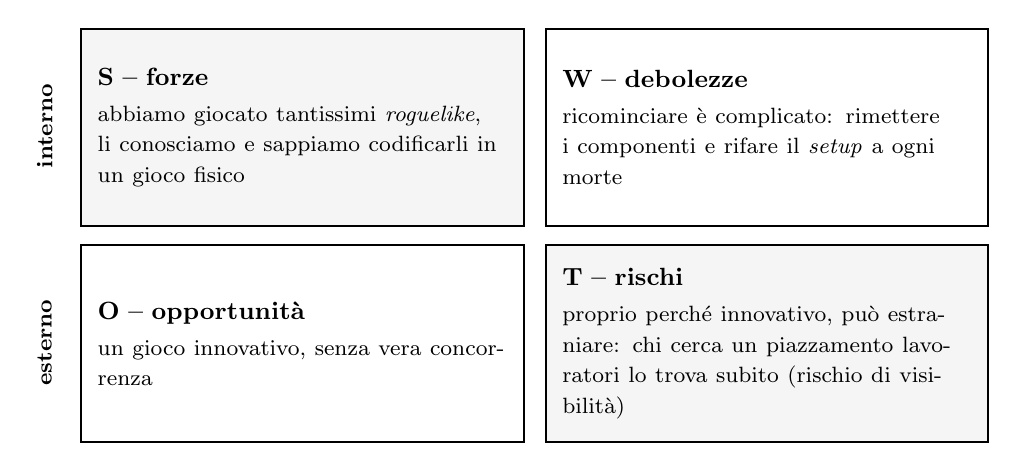
\begin{tikzpicture}[
  font=\small,
  a14q/.style={draw, thick, text width=5.2cm, minimum height=2.5cm, align=left,
               inner sep=6pt, anchor=north west}
]
  \node[a14q, fill=gray!8] (S) at (0,0) {\textbf{S -- forze}\\[2pt]\footnotesize abbiamo
    giocato tantissimi \emph{roguelike}, li conosciamo e sappiamo codificarli in un gioco
    fisico};
  \node[a14q] (W) at (5.9,0) {\textbf{W -- debolezze}\\[2pt]\footnotesize ricominciare è
    complicato: rimettere i componenti e rifare il \emph{setup} a ogni morte};
  \node[a14q] (O) at (0,-2.75) {\textbf{O -- opportunità}\\[2pt]\footnotesize un gioco
    innovativo, senza vera concorrenza};
  \node[a14q, fill=gray!8] (T) at (5.9,-2.75) {\textbf{T -- rischi}\\[2pt]\footnotesize
    proprio perché innovativo, può estraniare: chi cerca un piazzamento lavoratori lo
    trova subito (rischio di visibilità)};
  \node[rotate=90, font=\footnotesize\bfseries] at (-0.45,-1.25) {interno};
  \node[rotate=90, font=\footnotesize\bfseries] at (-0.45,-4.0) {esterno};
\end{tikzpicture}
\caption{L'analisi SWOT ``fatta in 30 secondi'' da Marta sull'esempio di un
\emph{roguelike} da tavolo. La riga in alto riguarda il progetto, quella in basso il mercato
di riferimento, inteso in senso largo (anche le persone che consultano itch.io). Le
categorie si leggono poi a coppie.}
\label{a14:fig:swot}
\end{figure}

\paragraph{Uno strumento si impara usandolo.} Ogni strumento visto oggi diventa più utile
\textbf{quanto più spesso lo si usa}. ``Non so se vi dilettate in cucina'', ma ci sono
tantissimi strumenti per cucinare, e più si usa uno strumento, più se ne conoscono limiti e
forze. Vale anche per la SWOT: ``la prima volta che la farete sarà una roba un po'
posticcia''; poi, man mano che la si sfrutta, si scoprono le sue utilità, soprattutto nel
\textbf{riassumere in breve} questi quattro punti.

% ---------------------------------------------------------------------
\section{Le \emph{personas}}
\label{a14:sec:personas}

\slidefig{img/AGD/agd14-personas}{Un esempio di persona.}{slide \emph{Tecniche di sviluppo}}{fig:agd14-personas}


Un altro strumento ``molto utile, sempre un po' mutuato da altri campi'', sono le
\textbf{\emph{personas}}, già accennate parlando di \emph{target}. ``Queste le conoscete?''
``Di nome, ma meno.''

\paragraph{Dal \emph{target} a una persona.} Quando si fa un gioco si ha in mente un
\emph{target}, ma i \emph{target} sono \textbf{misure astratte}: si può dire che un gioco è
``per gli appassionati'', ma ``se io dico appassionati, non ho in mente una persona''. Aiuta
invece avere \textbf{riferimenti molto specifici}. Siccome è difficile pensare in concreto a
una persona precisa che vuole il nostro gioco, si può ricorrere alle \emph{personas}, che
sono ``niente di più che'' \textbf{profili creati da noi}, popolati il più possibile.
Generalmente si costruiscono partendo da \textbf{dati molto generici} e poi
\textbf{scendendo nei dettagli}, stabilendo sempre di più i tratti di questa persona virtuale.

\paragraph{L'esempio della slide.} Nell'esempio della slide non c'è niente che non sia
definito in modo certo: la persona ha un \textbf{nome}\footnote{Nella trascrizione il nome è
prima ``Tian'' e poi ``Diane''; l'occupazione è ``e share consultant'', forse \emph{HR
consultant}. La slide non è nella trascrizione e il capitolo non può verificarlo.},
un'\textbf{età} (48 anni), un'\textbf{occupazione} (una consulente) e una \textbf{biografia},
una \emph{backstory} che racconta le cose che fa ogni giorno. Che cosa c'entrano con un gioco
da tavolo? ``Tendenzialmente, di base, niente.'' Ma anche per una persona reale le cose che fa
nella vita c'entrano poco con i suoi hobby; eppure ci aiutano a immaginare \textbf{che cosa
farebbe quella persona seduta a un tavolo da gioco}. Costruire una \emph{persona} dà una
dimensione e permette di \textbf{rispondere a delle domande}, del tipo: ``Diane giocherebbe
a \emph{I Coloni di Catan}?''\footnote{Nella trascrizione ``colonie di Katan''.} Più la
\emph{persona} è definita, più è probabile riuscire a rispondere.

\paragraph{Il rischio dei \emph{bias}.} Per la SWOT come per le \emph{personas}, il rischio è
che \textbf{i propri \emph{bias} condizionino il lavoro}. ``È un rischio che c'è sempre.''
L'invito è a essere persone \textbf{aperte} il più possibile, \textbf{curiose}, e a
\textbf{conoscere più persone possibile}: dà un vantaggio, e aiuta a calarsi negli altri con
più facilità.

\paragraph{\emph{Personas} costruite sui dati.} A seconda dell'entità del progetto, si possono
\textbf{raccogliere dei dati} e costruire le \emph{personas} su quei dati: fare dei campioni
quantitativi, per esempio con \textbf{un sondaggio}, per capire abitudini diffuse e interessi
condivisi di un certo \emph{target}. ``Magari a volte vi è capitato di fare un sondaggio'' che
chiedeva ``sei appassionata di giochi da tavolo?'' e poi ``quali libri leggi?'': ``e tu dici:
ok, ma che c'entra?''. A volte serve proprio a costruire questi profili.

\paragraph{Riusarle o no?} Uno degli inviti che si leggono spesso è a \textbf{non usare le
stesse \emph{personas} per più di un progetto}. Marta non la trova una regola necessariamente
funzionale: le è capitato di riusare le stesse \emph{personas} per più progetti, ``e
sinceramente non capisco bene il perché di no''. Riporta comunque quello che ha letto quando
ha imparato la tecnica: ognuno veda se gli torna utile.

\paragraph{Approfondimento: \emph{personas} e modelli di pubblico.} Bateman e Boon partono da
un modello di pubblico ancora più grezzo di quello che Marta chiama ``gli appassionati'': la
divisione tra giocatori \emph{hardcore} e \emph{casual}, che definiscono una ``ipotesi
consensuale'', accettata da quasi tutti nell'industria ma senza una definizione formale. Il
loro esempio è \emph{Resident Evil} per GameCube, che all'inizio chiedeva al giocatore se
preferisse ``scalare la montagna'' (oltre le fatiche c'è il risultato) o ``fare
un'escursione'' (la meta si raggiunge comodamente), per regolare la difficoltà. Le
\emph{personas} fanno il passo successivo: invece di due etichette, una persona con un nome,
un'età e una giornata, a cui fare domande concrete.

% ---------------------------------------------------------------------
\section{I sei cappelli per pensare}
\label{a14:sec:cappelli}

\slidefig{img/AGD/agd14-cappelli}{I sei cappelli per pensare.}{slide \emph{Tecniche di sviluppo}}{fig:agd14-cappelli}


``I sei cappelli per pensare. Questa forse la conoscete anche dal \emph{design}''. Qualcuno
l'ha sentita nominare; una voce, probabilmente di una studentessa, ricorda che nei suoi studi di \emph{design} se ne
parlava, ``ma non tramite i cappelli colorati'': il processo creativo analizzato da altri
punti di vista, ``però è molto interessante anche così''.

\paragraph{La prima pausa.} A questo punto Marta resta bloccata fuori dalle slide: ha aperto
la chat di Zoom e non riesce più a tornare alla presentazione (``vi giuro che non sono mai
stata così in difficoltà'', ``ho anche una laurea in informatica''; ``e ho fatto l'errore di
aprire la chat, non lo farò mai più''). Gli studenti continuano a vedere le slide, ma lei non
riesce a farle avanzare, e propone \textbf{dieci minuti di pausa} per risolvere. La pausa,
nella trascrizione, è coperta da frasi ripetute senza senso. Al ritorno: ``nel frattempo ho
trovato il modo di aprire la chat senza distruggere mezzo computer''.

\paragraph{A che cosa servono.} I sei cappelli sono un altro dei processi per
\textbf{calarsi in panni che non sono i propri}, utili soprattutto per figurarsi prospettive
che non sono quelle che vengono ``di primo acchito'' quando si lavora a un progetto. I
cappelli guardano a problemi simili \textbf{da punti di vista diversi}, e alcuni sono
volutamente \textbf{opposti}. Si possono usare in molti modi; Marta, per esempio, ha
\textbf{un mazzetto di sei carte}: le mescola, ne estrae una e si mette figurativamente quel
cappello. Si possono usare anche \textbf{in \emph{team}}: ognuno indossa un cappello, e poi
i cappelli \textbf{ruotano} per cambiare punto di vista. La tabella~\ref{a14:tab:cappelli}
li riassume.

\begin{description}
  \item[Il bianco: i fatti.] Guarda le cose \textbf{da un punto di vista neutrale}: asserisce
        i fatti nel modo più oggettivo possibile, si astiene dai giudizi e dà informazioni
        ``il più possibile dritte''. Per esempio: ``durante il \emph{playtest} è successa
        questa cosa'', senza dire se è positiva o negativa; ``si è verificato un paio di
        volte questo avvenimento''. Prende i dati in modo \textbf{distaccato}.
  \item[Il nero: i rischi.] Fa leva su \textbf{difficoltà, insicurezze, pericoli}: tutto
        quello che potrebbe non essere andato o potrebbe non andare. È uno dei cappelli
        \textbf{più facili da indossare}, perché è facile vedere le parti negative di un
        progetto. Proprio per questo invita a essere \textbf{più descrittivi}: non limitarsi
        a dire qual è la difficoltà, ma esplorarla e analizzarla nel dettaglio.
  \item[Il rosso: le emozioni.] Fa riferimento alle \textbf{emozioni}: come ci si sente
        quando lo si indossa, quali emozioni sono state provate. A differenza del nero,
        \textbf{non dà spiegazioni}: dice ``io mi sento così''. È un cappello molto utile e
        \textbf{spesso sottovalutato}, perché c'è la credenza che le emozioni valgano meno
        dei fatti; in realtà le emozioni guidano a capire qual è \textbf{l'esperienza
        desiderata}, che cosa si vuole ottenere da un \emph{design}, e se il \emph{design} lo
        sta facendo emergere.
  \item[Il giallo: i punti di forza.] È l'opposto del nero: elenca \textbf{le cose positive},
        i punti di forza, gli aspetti che esaltano l'esperienza. Anche questo è abbastanza
        semplice da indossare; anche qui l'invito è a ``lasciarsi andare'' sulle
        \textbf{ragioni} per cui quei punti sono di forza, e a sviscerarle.
  \item[La creatività.] Uno dei due cappelli ``più particolari''\footnote{Marta non dice il
        colore di questo cappello. Nel metodo originale di Edward de Bono (\emph{Six Thinking
        Hats}, 1985) il cappello della creatività è il \textbf{verde}.}: significa
        \textbf{lanciarsi in soluzioni anche esagerate e irrealistiche}. È il cappello del
        \textbf{\emph{brainstorming}}: si analizzano le possibilità, anche quelle fuori dagli
        schemi. Non importa se sono fattibili: il lavoro della creatività è \textbf{proporre
        idee}, soluzioni, possibilità; pensare a quali e quante sono, e cercare quelle più
        inusuali.
  \item[Il blu: l'organizzazione.] Il più particolare. In \emph{team} serve a
        \textbf{gestire gli altri cappelli}: chi indossa il blu stabilisce quando si cambia
        cappello. E inoltre dice: ``ok, però che cosa faremo? Che cosa implementeremo? Che
        cosa serve adesso per raggiungere gli scopi che ci prefiggiamo?''. È la parte
        \textbf{organizzativa} del processo, quella che segue la parte pratica una volta
        individuate le caratteristiche.
\end{description}

Nel complesso, i cappelli sono anche un modo di \textbf{dividere i pensieri in compartimenti
stagni}, ``e a volte questa cosa torna particolarmente utile''.

\begin{table}[htbp]
\centering
\small
\begin{tabular}{@{}p{2.3cm}p{3.6cm}p{3.9cm}p{3.7cm}@{}}
\toprule
\textbf{Cappello} & \textbf{Guarda a} & \textbf{Esempio di frase} & \textbf{Attenzione} \\
\midrule
Bianco & i fatti, neutri & ``durante il \emph{playtest} è successo due volte X'' & niente
  giudizi \\
\addlinespace
Nero & difficoltà, insicurezze, pericoli & ``questo potrebbe non funzionare perché\ldots'' &
  facile da indossare: va approfondito \\
\addlinespace
Rosso & le emozioni & ``io mi sento così'' & niente spiegazioni; spesso sottovalutato \\
\addlinespace
Giallo & i punti di forza & ``questo esalta l'esperienza perché\ldots'' & facile: andare a
  fondo delle ragioni \\
\addlinespace
Creatività (verde) & idee e soluzioni, anche irrealistiche & ``e se\ldots?'' & non giudica
  la fattibilità \\
\addlinespace
Blu & l'organizzazione: quando cambiare, che cosa fare ora & ``che cosa implementiamo?'' &
  in \emph{team}, gestisce gli altri \\
\bottomrule
\end{tabular}
\caption{I sei cappelli per pensare come li presenta Marta. Si possono pescare da un mazzetto
di sei carte, da soli, o far ruotare in un \emph{team}.}
\label{a14:tab:cappelli}
\end{table}

% ---------------------------------------------------------------------
\section{Il bilanciamento secondo Garfield}
\label{a14:sec:garfield}

\slidefig{img/AGD/agd14-bilancia}{Il bilanciamento.}{slide \emph{Tecniche di sviluppo}}{fig:agd14-bilancia}


``Ecco, ce l'ho fatta'': la slide successiva è il \textbf{bilanciamento}. ``Questo è il capitolo
un po' più complicato da fare, ma vedremo perché.'' Marta raccomanda di interromperla con le
domande, perché è ``un argomento molto spesso spinoso'', e lei lo tratta ``in un modo un po'
atipico rispetto ai miei colleghi''.

\paragraph{\emph{The Balancing Act}.} Si parte da uno degli articoli che da qualche anno sono
diventati un punto di riferimento per il suo lavoro, scritto ``niente di meno che'' da
\textbf{Richard Garfield}\footnote{Marta cita il titolo dell'articolo, \emph{The Balancing
Act}, ma non dice dove sia stato pubblicato; il capitolo non lo ha verificato. Le citazioni
che seguono sono la parafrasi italiana di Marta dalla slide, non il testo originale.}. Lo si
troverà citato spesso: Garfield è un designer con un'esperienza ormai
\textbf{quarantennale} (``ormai sono 40 anni, direi''), con tantissimi giochi di successo,
``non c'è solo \emph{Magic}'', e ha una profonda conoscenza non solo del gioco ma di tutto
ciò che gli ruota attorno. ``Secondo me è un'ottima lettura a prescindere'': molto spesso è
stato \textbf{sottovalutato}, perché molti lo associano solo a \emph{Magic}, ``e invece ha
fatto tanto, tanto di più''. Nell'articolo Garfield esorta così:
\begin{quote}
\textbf{il bilanciamento perfetto dei giochi è un mito. Il bilanciamento consiste nel
migliorare il \emph{play}, il giocare, per un ampio spettro di possibili giocatori, e
comporta costi e benefici.}
\end{quote}
È una frase che, per Marta, riassume perfettamente tanti punti del bilanciamento. La parte che
molti dimenticano è quella dei \textbf{costi e benefici}: qualsiasi bilanciamento si operi
presenterà, ``se vogliamo, anche per ricondurci all'analisi SWOT'', delle forze, delle
debolezze, delle opportunità e dei rischi.

\paragraph{Un'esplorazione dello spazio di gioco.} Che cos'è, allora, il bilanciamento? Si
può definire come \textbf{l'esplorazione di una parte dello spazio di gioco totale}. Dato un
gioco, applicando bilanciamenti diversi, e anche regole diverse, se ne esplora una parte
diversa. Quando si presenta un gioco sviluppato, finito, si sta implicitamente consegnando
\textbf{una porzione di uno spazio di gioco molto più ampio} (figura~\ref{a14:fig:spazio}).

\paragraph{Non esiste un bilanciamento che accontenti tutti.} Si pensa che questa porzione
debba accontentare tutti, ma, proprio per i costi e benefici, non è così. Molto spesso chi
segue il principio di accontentare tutti \textbf{sta accontentando soltanto la parte più
rumorosa dell'utenza}: quella che si esprime in modo più vocale, spesso non da una posizione
di conoscenza, ma perché è molto facile giudicare un gioco; e ``quindi molto spesso si
prendono dei granchi''. \textbf{Abbandonare l'idea che un gioco possa risultare adatto a
chiunque} è, per Marta, l'obiettivo da avere quando ci si mette sotto con lo sviluppo: ``non
esistono giochi che sono adatti a tutte le persone''.

\begin{figure}[htbp]
\centering
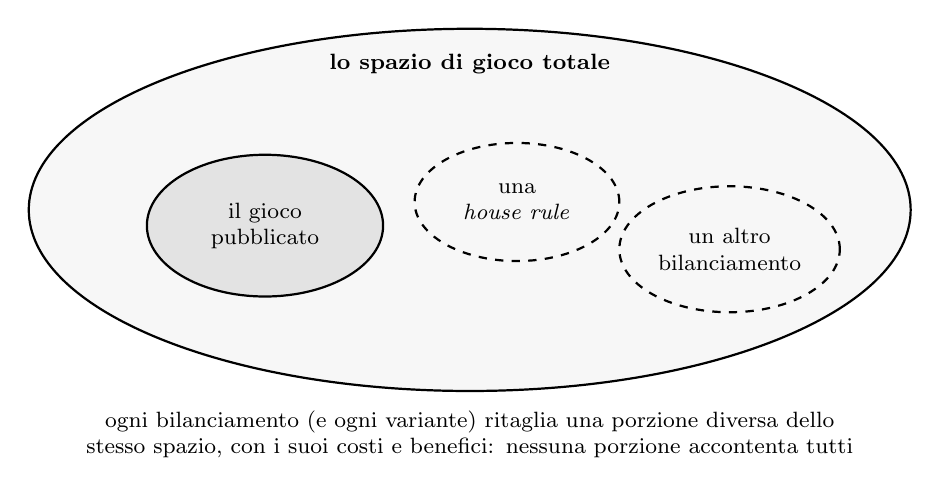
\begin{tikzpicture}[font=\small]
  \draw[thick, fill=gray!6] (0,0) ellipse (5.6cm and 2.3cm);
  \node[font=\footnotesize\bfseries] at (0,1.85) {lo spazio di gioco totale};
  \draw[thick, fill=gray!22] (-2.6,-0.2) ellipse (1.5cm and 0.9cm);
  \node[align=center, font=\footnotesize] at (-2.6,-0.2) {il gioco\\pubblicato};
  \draw[thick, dashed] (0.6,0.1) ellipse (1.3cm and 0.75cm);
  \node[align=center, font=\footnotesize] at (0.6,0.1) {una\\\emph{house rule}};
  \draw[thick, dashed] (3.3,-0.5) ellipse (1.4cm and 0.8cm);
  \node[align=center, font=\footnotesize] at (3.3,-0.5) {un altro\\bilanciamento};
  \node[font=\footnotesize, text width=10cm, align=center] at (0,-2.85) {ogni bilanciamento
    (e ogni variante) ritaglia una porzione diversa dello stesso spazio, con i suoi costi e
    benefici: nessuna porzione accontenta tutti};
\end{tikzpicture}
\caption{Il bilanciamento come esplorazione dello spazio di gioco: il gioco finito ne
consegna una porzione; le \emph{house rules} e le varianti, nell'analogico, permettono a chi
gioca di esplorarne altre.}
\label{a14:fig:spazio}
\end{figure}

\paragraph{Dare più potere a chi gioca.} Il mondo analogico ha una grande forza che nel
videogioco non è altrettanto facile: \textbf{se vogliamo cambiare una regola, basta dirlo
quando si spiegano le regole}. Nel videogioco, per farlo, servono di solito conoscenze di
programmazione o di progettazione che vanno al di là di quello che l'utenza comune riesce a
fare. Il gioco analogico dà invece uno strumento molto forte: \textbf{varianti} e
\textbf{\emph{house rules}}, per tarare il gioco sul proprio livello.

\paragraph{Il gioco non è un artefatto immutabile.} Marta spende ``altre due parole''. C'è una
tendenza, che lei stessa ha seguito per tanti anni, a pensare al gioco come a un
\textbf{artefatto immutabile}: è stato fatto così e non può essere toccato. Esiste in molti
ambiti, per esempio con i libri, che molte persone non vogliono assolutamente modificare,
segnare, sottolineare. È una concezione che Marta si prende la libertà di definire ``molto
orientata al capitalismo'', in cui gli oggetti non sono davvero propri ma entità da
preservare per preservarne il valore. I \textbf{giochi \emph{legacy}} aiutano a svincolarsi
da questo principio. \textbf{Lavorare su un gioco e metterci del proprio è il gesto di
possesso più forte che si possa fare}, e in un certo senso anche un gesto d'amore: se si
modifica un gioco con \emph{house rules} e varianti, probabilmente è perché piace così tanto
che, piuttosto che bollarlo come ``non è un gioco per me'', si è disposti a
\textbf{esplorarne lo spazio di gioco}. È una cosa che nell'ambiente si è un po' persa, ma
che è sempre stata una caratteristica del gioco: Marta invita a riscoprirla, ``perché tira
fuori tante cose positive''.

\paragraph{Le \emph{house rules} come palestra di sviluppo.} Inoltre, praticare le \emph{house
rules} \textbf{spinge verso lo sviluppo}: toccare un gioco edito e vedere come cambia variando
le regole trasmette il \emph{feeling} di lavorare a un gioco già creato da qualcun altro e
metterci le mani sopra, cioè proprio il mestiere di chi sviluppa.

\paragraph{L'obiettivo: esaltare le forze, minimizzare gli ostacoli.} L'obiettivo del
bilanciamento è lo stesso dello sviluppo in generale: \textbf{esaltare le forze del
\emph{design} e minimizzare gli ostacoli}. Non lo si pensi come il raggiungimento di un
\textbf{equilibrio perfetto}, che non esiste; ci si chieda sempre: ``ok, però questo
\emph{design} che cosa si promette di fare? Come faccio a veicolarlo?''.

% ---------------------------------------------------------------------
\section{Per chi si bilancia}
\label{a14:sec:perchi}

È importante ricordare \textbf{per chi} si sta facendo il bilanciamento. Potrebbero essere
persone \textbf{esperte}, appassionate; persone \textbf{alle prime armi}; o, a volte, ``il
\textbf{dio della simmetria}'', come lo chiamano dove lavora Marta.

\paragraph{Il dio della simmetria.} È quando ci si intestardisce che \textbf{i numeri debbano
finire tutti per 5 o per 10}, o che, siccome questa carta vale 2, \textbf{anche quella debba
valere 2}, senza contemplare per esempio i numeri dispari: ``sono tutte delle fisime che vengono
fuori quando si sviluppa''\footnote{Nella trascrizione ``sono tutte delle fisiche'': quasi
certamente ``fisime''.}. ``Io sono la prima che a volte ci cade, in questi tranelli'': l'ha
messo nella slide anche per prendersi in giro. Ma è un avvertimento serio: quando si bilancia,
si tende verso i propri \emph{bias}, e il dio della simmetria è uno di questi.

\paragraph{Bilanciare per il gioco.} A volte si bilancia \textbf{per il gioco}, cioè per il suo
interesse: il gioco vuole creare certe dinamiche, quelle infuse da chi l'ha creato, e
bilanciare per il gioco significa \textbf{non pensare necessariamente al \emph{target}}, ma a
come tirare fuori il più possibile l'esperienza. Vale soprattutto per i \textbf{giochi non
commerciali}, in cui l'interesse è portare l'esperienza anche a discapito dell'utenza, e per
i giochi \textbf{molto sperimentali}.

L'esempio è un gioco ``molto bello'' di \textbf{Amabel Holland}, in solitario, che si chiama
\textbf{\emph{Endurance}}\footnote{Il titolo e l'autrice sono detti chiaramente; editore e
anno non sono nominati. Amabel Holland pubblica di solito con Hollandspiele.}. Ricrea le
vicende della spedizione dell'\emph{Endurance}, ``una spedizione miracolosa'' in cui i membri
dell'equipaggio si sono salvati dopo una quantità immensa di tempo passato, ``se non
sbaglio'', in Antartide\footnote{È la spedizione imperiale transantartica di Ernest
Shackleton (1914--1917): la nave \emph{Endurance} rimase intrappolata nei ghiacci e affondò,
e tutto l'equipaggio sopravvisse dopo quasi due anni.}. Quello che Holland ha voluto ricreare
è che, quando si gioca, \textbf{nel 99\% dei casi si perde}, perché l'equipaggio muore.
``Perdere'' è un'imprecisione: nel gioco \textbf{non ci sono vere condizioni di vittoria o di
sconfitta}, ma un'analisi di quello che è successo e un racconto dell'esperienza. La storia in
cui tutti si salvano è \textbf{volutamente rarissima}, per dimostrare la straordinarietà
dell'evento reale e ricalcare la difficoltà di ottenere un risultato del genere. Qui si
bilancia per il gioco, anche se il \emph{target} potrebbe non apprezzarlo; o meglio, c'è un
\emph{target} ``un po' più nascosto'' di quello commerciale.

\paragraph{Bilanciare per il \emph{target}.} È il discorso inverso: si bilancia per chi,
secondo noi, giocherà il gioco. Tendenzialmente si bilancia per il \emph{target}, ma nella
pratica è più difficile di quanto sembri, perché è facile \textbf{dimenticare che si sta
bilanciando per persone con interessi diversi dai nostri}, e finire a bilanciare per noi
stessi. L'esempio che aiuta è quello dei \textbf{giochi per bambini}: lì ``chiaramente noi non
siamo bambini'', e la differenza salta all'occhio. Quando Marta ha lavorato a un gioco per
bambini chiamato \textbf{\emph{Sun Farm}}\footnote{Così nella trascrizione; il titolo non è
verificabile.}, il bilanciamento è partito \textbf{dai bambini e dai genitori}: capire quale
potesse essere l'esperienza desiderata da un bambino, e perché in quel caso \textbf{vincere
non era la cosa più importante dell'universo}, mentre contavano di più
l'\textbf{espressività} e la possibilità di giocare un po' con le strategie senza restringere
il campo delle possibilità.

\paragraph{Esperti o principianti.} C'è spesso la tendenza a fare giochi \textbf{solo per i
giocatori migliori}, o per quelli che sono vocali e si spacciano per i migliori. Molto spesso
sono persone che \textbf{il gioco l'hanno giocato pochissimo}: sui gruppi e sui \emph{forum}
si trovano persone che dicono ``questo gioco è rotto'' dopo una partita. È una tendenza che
c'è anche \textbf{nell'industria}, dietro le quinte, tra addetti ai lavori; ``posso ammettere
che anche io l'ho fatto''. Ed è, come dice anche Garfield, \textbf{profondamente
irrispettoso}: si pensa che il gioco sia fatto solo per noi, quando magari non siamo
minimamente nel suo \emph{target}, o il gioco richiede competenze che non abbiamo o non
abbiamo voglia di applicare. Bisogna ricordarsi che \textbf{un gioco non è giocato soltanto
da queste persone}: è giocato da tantissime persone che non commentano sui \emph{forum}, non
scrivono su BGG, non lasciano voti. E il gioco deve essere \textbf{accessibile al maggior
numero possibile di persone}, proprio perché arrivi anche nelle mani di chi non si esprime ma
avrebbe piacere di giocarlo.

\paragraph{Tecnicità contro approcciabilità.} Per riassumere: da una parte si bilancia
\textbf{per tecnicità}, per rendere il gioco ``più bello'', e magari non si riesce ad
accontentare nessuno, perché per $N$ persone che si lamentano ce ne saranno $M$ che si
lamenteranno una volta fatta la modifica. Dall'altra si bilancia \textbf{per
approcciabilità}, per rendere il gioco più approcciabile: questo \textbf{allarga la base
d'utenza} che può accedere al gioco e favorisce che venga effettivamente provato. Marta
precisa, ``fatemi sapere se non vi è chiara la differenza'': \textbf{non significa che non si
possano fare giochi complessi}, o impegnativi. ``Non è questo il punto del discorso.''

% ---------------------------------------------------------------------
\section{Perché non bilanciare (solo) con la matematica}
\label{a14:sec:matematica}

Perché, allora, non si bilancia spesso \textbf{``in modo matematico''}, come si dice? Marta
elenca le ragioni.

\paragraph{È lungo e soggetto a errori.} Non conosce le competenze matematiche di tutte le
persone che si avvicinano al \emph{design} e allo sviluppo, ma nella sua esperienza vede
molto spesso \textbf{ragionamenti matematici fallaci}, che ``non stanno in piedi''. Ed è un
processo \textbf{lungo e faticoso}, che porta a sbagliare tantissime volte. A meno di essere
``davvero, davvero, davvero molto in gamba'' su questo aspetto, va affrontato con cautela.

\paragraph{È difficilmente modellabile.} Molto spesso \textbf{i modelli sono sbagliati}:
quando si cerca di sintetizzare un gioco si perdono \textbf{le dipendenze tra le risorse}, le
\textbf{transazioni} da una risorsa all'altra, da una carta all'altra. E si perde quello che
rende i giochi affascinanti: i cosiddetti \textbf{spazi di permeabilità}, già nominati
``ieri'', che \textbf{neanche il designer conosce sempre in modo approfondito} e che fanno la
differenza. I giochi sono interessanti proprio perché sono sistemi \textbf{non pienamente
controllati, non pienamente compresi}. Si pensi agli \textbf{scacchi}: chi li ha progettati
non aveva ``minimamente idea'' di tutto quello che è venuto dopo; molte innovazioni
strategiche sono degli ultimi cinquant'anni. È notevole quanti spazi di permeabilità avesse,
grazie alla struttura aperta del suo albero decisionale, ``che, penso lo sapete, è
immenso''.

\paragraph{Appiattisce le scelte.} Bilanciare in modo matematico porta a un
\textbf{appiattimento delle scelte}, perché si tende a trovare degli \textbf{equilibri
statici}: si immagini una bilancia perfettamente in equilibrio. Ne nascono le famose
\textbf{scelte indifferenti}: qualsiasi cosa si faccia, la ricompensa è identica. Un percorso
dà 1 punto vittoria al primo turno, 3 al secondo e 2 al terzo; un altro ne dà 1 al primo, 2 al
secondo e 3 al terzo. Alla fine \textbf{sono 6 punti per tutte e due le strade}: ``quindi
abbiamo risolto assolutamente niente'' (figura~\ref{a14:fig:indifferenti}). L'esperienza
diventa \textbf{statica e priva di significato}.

\begin{figure}[htbp]
\centering
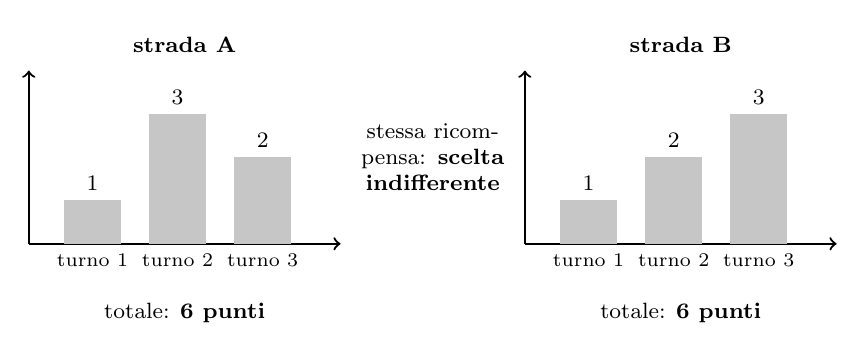
\begin{tikzpicture}[font=\small, x=0.9cm, y=0.55cm]
  % assi
  \foreach \ox/\tit/\a/\b/\c in {0/{strada A}/1/3/2, 7/{strada B}/1/2/3}{
    \draw[thick, ->] (\ox,0) -- (\ox+4.4,0);
    \draw[thick, ->] (\ox,0) -- (\ox,4.0);
    \node[font=\footnotesize\bfseries] at (\ox+2.2,4.6) {\tit};
    \fill[gray!45] (\ox+0.5,0) rectangle (\ox+1.3,\a);
    \fill[gray!45] (\ox+1.7,0) rectangle (\ox+2.5,\b);
    \fill[gray!45] (\ox+2.9,0) rectangle (\ox+3.7,\c);
    \node[font=\footnotesize, above] at (\ox+0.9,\a) {\a};
    \node[font=\footnotesize, above] at (\ox+2.1,\b) {\b};
    \node[font=\footnotesize, above] at (\ox+3.3,\c) {\c};
    \node[font=\scriptsize, below] at (\ox+0.9,0) {turno 1};
    \node[font=\scriptsize, below] at (\ox+2.1,0) {turno 2};
    \node[font=\scriptsize, below] at (\ox+3.3,0) {turno 3};
    \node[font=\footnotesize] at (\ox+2.2,-1.6) {totale: \textbf{6 punti}};
  }
  \node[font=\footnotesize, text width=2.4cm, align=center] at (5.7,2.0) {stessa
    ricompensa: \textbf{scelta indifferente}};
\end{tikzpicture}
\caption{L'esempio di Marta di scelte indifferenti, prodotto da un bilanciamento matematico
``statico'': due percorsi con andamenti diversi ma lo stesso totale. Scegliere l'uno o
l'altro non cambia niente.}
\label{a14:fig:indifferenti}
\end{figure}

``Anche qua'', precisa, ``non significa che non si usa la matematica'': la matematica aiuta e
può tornare comoda sotto molti aspetti. Ma bisogna fare attenzione a \textbf{non guardare il
bilanciamento solo da questo punto di vista}, perché è una tendenza comune a chi si avvicina al
bilanciamento e porta a degli errori.

\paragraph{Il bilanciamento esperienziale.} Marta consiglia sempre il \textbf{bilanciamento
esperienziale}: veicolare \textbf{i percorsi intesi}, l'obiettivo del \emph{design}. Che cosa
si prefigge il gioco? Quali strade voglio che siano percorse a livello strategico? Che cosa
voglio \textbf{premiare}? Costruire le \textbf{scelte sensibili}, cioè indirizzare le scelte
delle persone verso alcune delle idee e delle strategie che si vogliono mettere in campo, e
lasciare che il \emph{gameplay} sia \textbf{emergente}, che consenta anche a chi gioca di
metterci del proprio. Il bilanciamento esperienziale è anche \textbf{parametrizzabile}: se tra
gli \emph{stakeholder} c'è chi vuole un gioco ``un po' più cattivo'', che restituisca un
\emph{feeling} di frustrazione, lo si può fare senza problemi; il bilanciamento matematico
molto spesso lo impedisce, perché tende a equalizzare tutto su un livello statico.

\paragraph{E l'intelligenza artificiale?} Un tema diventato rilevante quest'anno, ``l'anno
scorso lo era un po' meno'': molte persone \textbf{bilanciano con l'intelligenza
artificiale}. Marta non si mette a spiegare come funziona, ``però insomma, non è una cosa che
veramente pensi, mettiamola così: è semplicemente un \textbf{algoritmo predittivo}''. Molto
spesso porta proprio agli \textbf{errori del bilanciamento matematico}. Il suo invito è a
\textbf{non usarla}; ma chi la usa faccia attenzione, perché può portare a un bilanciamento
``assolutamente errato e che appiattisce il gioco''.

\paragraph{Approfondimento: il modello e il gioco.} Schell non è contrario ai modelli, ma ne
descrive bene il limite: ``il modello informa il bilanciamento, e il bilanciamento informa il
modello''. Si scrive il proprio modello di come sono legate le meccaniche, lo si mette alla
prova giocando, e lo si corregge ogni volta che il gioco non si comporta come previsto.
Aggiunge che il bilanciamento può cominciare davvero solo quando il gioco è giocabile, e che
la sua regola personale è dedicare al bilanciamento \textbf{metà del tempo di sviluppo}. È la
stessa direzione di Marta: i numeri servono, ma come ipotesi da verificare al tavolo, non come
risposta.

% ---------------------------------------------------------------------
\section{Come cominciare: giochi a scarsa interazione}
\label{a14:sec:cominciare}

Un consiglio per chi vuole iniziare a sperimentare con il bilanciamento: partire da
\textbf{giochi a scarsa interazione}. I giochi ad alta interazione hanno tante
\textbf{interdipendenze} con quello che fanno i giocatori; si possono modellare anche
matematicamente, soprattutto in termini probabilistici, ``ma è molto complesso''. Partire da
giochi con poca interazione permette di lavorare in modo più agevole. Marta precisa che sta
parlando soprattutto di giochi con \textbf{un modello matematico alle spalle}: giochi con
\textbf{conversioni di risorse}, in cui si vince a \textbf{punti vittoria}; non tanto di giochi
narrativi. Nel mondo del gioco da tavolo c'è ancora una preponderanza di questo tipo di giochi,
e quando si parla di bilanciamento si parla di solito di questo, anche se, come detto la volta
prima, non è affatto l'unico che si fa.

\paragraph{Modellare il sistema.} Partendo da un gioco a scarsa interazione, si prova a
\textbf{modellarne il sistema}: capire le \textbf{dipendenze} tra le risorse, con un
\textbf{diagramma di flusso} o anche un \textbf{diagramma di stato}, se torna utile.
L'obiettivo è individuare il \textbf{percorso che fanno le risorse}: quando vengono prese,
quando vengono restituite, e così via.

\paragraph{Un esempio: \emph{Splendor} infinito.} Si può partire da \textbf{\emph{Splendor}} e
immaginarlo con \textbf{risorse infinite}: le fiche di ogni colore sono infinite, e le carte
sono in $N$ copie, quindi possono essere sempre prese. Si prova a bilanciare da lì e si vede
che succede.

\paragraph{Variare i parametri.} Si testa come varia il gioco al variare dei parametri,
semplicemente \textbf{cambiando i parametri}, anche in modo arbitrario (tra poco si vedranno
alcune tecniche). Per esempio: che succede se, in \emph{Splendor}, una delle risorse, la
carta, diventa \textbf{esclusiva}, e non più in $N$ copie?

\paragraph{I \emph{test} in solitaria e il \emph{groupthink}.} I \emph{test} in solitaria qui
sono agevoli, ma attenzione al \textbf{\emph{groupthink}}, soprattutto se se ne fanno molti
durante il bilanciamento: ragionando da soli capita molto spesso di \textbf{rinforzare i
propri \emph{bias}}, e può diventare un problema, soprattutto se non si è consapevoli di
averli. Bisogna testare con \textbf{più persone}, e potenzialmente con \textbf{più gruppi
possibili}, per capire come si assesta il bilanciamento ed evitare il fenomeno.

\paragraph{Lasciare gli spazi di permeabilità.} ``Mi raccomando'': non bisogna avere
\textbf{l'ansia di controllare tutto il sistema di gioco}; non è necessario.

\paragraph{La strategia dominante emerge.} Se c'è una \textbf{strategia dominante}, di solito
la si intuisce analizzando il gioco da diversi punti di vista, o anche banalmente con i
\emph{playtest}: con un numero sufficiente di partite, i comportamenti emergono. L'esempio più
popolare: \textbf{tenere traccia di chi inizia a giocare} e vedere se è la persona che vince.
Se lo è, c'è un problema: chi inizia magari vince perché \textbf{fa un turno in più} degli
altri (``generalmente questo può essere uno dei motivi'').

% ---------------------------------------------------------------------
\section{Il budget di complessità}
\label{a14:sec:budget}

Uno dei concetti che tornano molto utili nello sviluppo, e che si trovano spesso soprattutto
nel bilanciamento, è il \textbf{budget di complessità}. Un gioco ha una certa complessità, un
certo grado di difficoltà: non la si immagini necessariamente come un numero, ma comunque come
\textbf{una quantità}, una quantità $x$. Quando si lavora al gioco, \textbf{rimuovere o
cambiare delle parti altera il budget}. Generalmente, togliendo per esempio una meccanica, si
\textbf{guadagna} complessità disponibile. E che cosa ci si fa, con questo guadagno?
\begin{itemize}
  \item lo si può semplicemente \textbf{togliere}, riducendo la complessità generale
        dell'esperienza;
  \item oppure lo si può \textbf{investire} altrove.
\end{itemize}

\paragraph{L'esempio del mercato azionario.} Si immagini un gioco con un obiettivo molto
definito: far sperimentare a chi gioca \textbf{come varia il mercato azionario}. Sul tavolo ci
sono i vari beni messi sul mercato, e bisogna rappresentare questo aspetto. Se il gioco ha
anche una \textbf{fase d'asta}, sta concentrandosi sull'asta: oltre ad aggiungere complessità,
\textbf{toglie \emph{focus}} alle fluttuazioni di mercato, cioè al comprare e vendere.
Togliendo l'asta si riduce la complessità; e quello che si è guadagnato lo si può usare per
rendere \textbf{un po' più complessa} la parte del mercato: il comprare, il vendere, il variare
dei prezzi dei beni. Il gioco diventa \textbf{più focalizzato}, più centrato su ciò che vuole
rappresentare, al prezzo di aver tolto una meccanica, ma \textbf{senza aver necessariamente
ridotto il budget di complessità} (figura~\ref{a14:fig:budget}).

\paragraph{Nel dubbio, accessibile.} Se non si intuisce che c'è qualcosa da fare con la
complessità recuperata, ``chiaramente sappiate che è sempre meglio avere un gioco
\textbf{accessibile} laddove è possibile'': lo scoglio iniziale, cioè provare il gioco e
metterlo sul tavolo, diventa più semplice.

\begin{figure}[htbp]
\centering
\begin{tikzpicture}[font=\small, x=1cm, y=1cm]
  % prima
  \node[font=\footnotesize\bfseries] at (1.0,4.5) {prima};
  \draw[thick] (0,0) rectangle (2,4);
  \fill[gray!20] (0,0) rectangle (2,1.6);
  \node[font=\footnotesize] at (1,0.8) {asta};
  \fill[gray!45] (0,1.6) rectangle (2,3.6);
  \node[font=\footnotesize, align=center] at (1,2.6) {mercato};
  \node[font=\scriptsize] at (1,3.8) {altro};
  % opzione 1
  \node[font=\footnotesize\bfseries, align=center] at (5.2,4.5) {togliere e\\basta};
  \draw[thick] (4.2,0) rectangle (6.2,4);
  \fill[gray!45] (4.2,0) rectangle (6.2,2.0);
  \node[font=\footnotesize] at (5.2,1.0) {mercato};
  \node[font=\scriptsize] at (5.2,2.2) {altro};
  \node[font=\scriptsize, align=center] at (5.2,3.3) {budget\\libero};
  % opzione 2
  \node[font=\footnotesize\bfseries, align=center] at (9.4,4.5) {reinvestire\\nel focus};
  \draw[thick] (8.4,0) rectangle (10.4,4);
  \fill[gray!45] (8.4,0) rectangle (10.4,3.6);
  \node[font=\footnotesize, align=center] at (9.4,1.8) {mercato\\più ricco};
  \node[font=\scriptsize] at (9.4,3.8) {altro};
  \draw[-{Stealth[length=2.5mm]}, thick] (2.3,2) -- (3.9,2);
  \draw[-{Stealth[length=2.5mm]}, thick] (2.3,2.6) to[bend left=25] (8.1,2.6);
  \node[font=\footnotesize, text width=11cm, align=center] at (5.2,-0.7) {togliendo
    l'asta si libera complessità: la si può lasciare libera (gioco più accessibile) o
    spenderla dove il gioco vuole il suo \emph{focus}};
\end{tikzpicture}
\caption{Il budget di complessità nell'esempio di Marta del gioco sul mercato azionario.
L'altezza della colonna è il budget complessivo; i blocchi sono le parti del gioco che lo
consumano.}
\label{a14:fig:budget}
\end{figure}

% ---------------------------------------------------------------------
\section{Strategie ad alto e a basso rischio}
\label{a14:sec:rischio}

\slidefig{img/AGD/agd14-rischio}{Strategie ad alto e a basso rischio.}{slide \emph{Tecniche di sviluppo}}{fig:agd14-rischio}


Un altro concetto che torna spesso sono le \textbf{strategie ad alto e a basso rischio}. Quando
si bilancia, uno dei riferimenti può essere avere più strategie: alcune in cui si
\textbf{rischia tanto, ma la ricompensa è elevata}, e altre in cui il \textbf{rischio è
ridotto, ma la ricompensa è parziale}. È un esempio tipico di tecnica per creare
\textbf{scelte sensibili}: dove c'è una sola possibilità, creare questa \textbf{biforcazione}
aiuta a costruire una scelta, ``e per come è fatta funziona un po' sempre''.

\paragraph{Perché funziona.} La difficoltà sta nel \textbf{valutare il livello di rischio} e
quanto si vuole rischiare di volta in volta. E siccome noi umani \textbf{fatichiamo con il
calcolo delle probabilità}, questo nel gioco diventa una forza, ``una sorta di abilità che si
può allenare''. È uno degli strumenti da mettere a disposizione quando serve una dinamica con
\textbf{più strade per arrivare a un risultato}: due macro-strategie, una che lavora tendenzialmente
a basso rischio e una ad alto rischio. Le due strade \textbf{non sono separate}: magari ci sono
strategie definite, ma è sempre possibile \textbf{passare dall'una all'altra lungo il
percorso}, e questo crea una dinamica di gioco effettiva.

\paragraph{L'esempio su \emph{Splendor}.} Sempre partendo da \emph{Splendor}: posso prendere
\textbf{una carta senza vederla} da uno dei mazzi e \textbf{riservarmela in mano}. Potrebbe
essere una strategia ad alto rischio, ma magari è l'unico modo di arrivare a \textbf{un quarto
mazzo} con le ricompense più alte: perdo il turno rischiando di non trovare quello che mi
serve, ma intanto ho la possibilità di fare qualcosa che le altre carte non mi permettono.
Una strategia a basso rischio è invece giocare con quello che ho, magari con le carte del
primo livello\footnote{L'esempio è in parte ipotetico: in \emph{Splendor} si può davvero
riservare una carta a faccia in giù dalla cima di un mazzo (ricevendo un gettone oro), ma i
mazzi di sviluppo sono tre; il ``quarto mazzo'' con le ricompense più alte è un'aggiunta di
Marta per illustrare il principio.}.

\paragraph{Approfondimento: la triangolarità.} È la \emph{lente della triangolarità} di
Schell, già incontrata nella lezione precedente: offrire al giocatore la scelta tra una mossa
sicura a bassa ricompensa e una rischiosa ad alta ricompensa. Il suo esempio è \emph{Space
Invaders}: i nemici normali valgono pochi punti e sono facili da colpire, mentre la navicella
misteriosa che attraversa ogni tanto lo schermo vale molto di più, ma inseguirla espone al
pericolo. Schell aggiunge una domanda di controllo che si applica bene alla biforcazione di
Marta: il tentativo di triangolarità è bilanciato, cioè la ricompensa è commisurata al
rischio?

% ---------------------------------------------------------------------
\section{L'ancoraggio}
\label{a14:sec:ancoraggio}

\slidefig{img/AGD/agd14-ancoraggio}{L'ancoraggio.}{slide \emph{Tecniche di sviluppo}}{fig:agd14-ancoraggio}


Un'altra tecnica di bilanciamento è l'\textbf{ancoraggio}. Quando si vogliono bilanciare dei
valori, può essere utile vedere le risorse attraverso \textbf{un valore di riferimento}: c'è un
cosiddetto \textbf{valore ancora}, e \textbf{tutto il sistema viene rapportato a quel
valore}. Due avvertenze, perché la tecnica è molto matematica, molto legata alla gestione dei
numeri:
\begin{itemize}
  \item le \textbf{risorse interdipendenti} rischiano di non essere facili da modellare. Per
        esempio: quanto vale \textbf{un turno extra}, in termini di valore ancora? ``È un
        argomento un po' complesso, perché un turno quanto vale?'';
  \item attenzione ai \textbf{meccanismi autobilancianti}, come il \textbf{\emph{draft}} di
        carte, che molto spesso vanno in opposizione alla tecnica dell'ancoraggio.
\end{itemize}

\paragraph{Il caso \emph{Stone Age}.} Come si fa? Partendo da un gioco molto semplice,
\textbf{\emph{Stone Age}}. ``Non so se lo conoscete.'' Gli studenti non ricordano di averlo
visto a lezione. È un gioco ``abbastanza vecchio'', un classico \textbf{piazzamento
lavoratori}. La sua particolarità: si piazzano i propri omini sui vari spazi, e quando li si
riprende \textbf{si lanciano tanti dadi quanti omini} si sono usati per prendere quella risorsa.
Se, per esempio, sono il giocatore giallo e ho \textbf{4 omini sul legno}, li riprendo e lancio
\textbf{4 dadi}; sommo il risultato e lo \textbf{divido per 3}, cioè conto quante volte il 3 sta
nel numero che ho fatto: quelle sono le risorse legno che ottengo. \textbf{Con 4 dadi e un
totale di 9, ottengo 3 legni}.

\paragraph{Le capanne.} A un certo punto del gioco si possono costruire \textbf{le capanne}, che
danno un certo numero di punti, mostrati nella slide sotto le capanne. Marta fa notare (dopo
essersi corretta: ``oddio, scusate, ho fatto un errore'') che \textbf{il valore in punti di una
capanna è pari al suo costo di costruzione}: un legno vale 3, un altro legno 3, un oro 6, come
si vede dalla tabella; $3+3+6=12$, e questo è il valore della capanna. Da qui si intuisce che
\textbf{il valore ancora del gioco sono i puntini sul dado}: \textbf{un puntino sul dado equivale
a un punto vittoria}. Va convertito, perché non dà punti di per sé, ma è il valore a cui si
appoggia tutta la matematica sottesa del gioco. Infatti: $3+3+5=11$, $4+4+6=14$, e così via
(tabella~\ref{a14:tab:stoneage}). Ci sono anche \textbf{capanne con il punto interrogativo}:
quella della slide dice ``usa 5 risorse qualsiasi, ma di almeno 4 tipi diversi'', e il
punteggio è dato proprio dalla somma dei valori delle risorse spese. ``Quindi non è neanche così
nascosta, come informazione.''

\begin{table}[htbp]
\centering
\small
\begin{tabular}{@{}lcp{7.2cm}@{}}
\toprule
\textbf{Risorsa} & \textbf{Divisore = valore} & \textbf{Che cosa vuol dire} \\
\midrule
Cibo & 2 & (non usato per le capanne) \\
Legno & 3 & con 4 dadi e totale 9, si prendono 3 legni \\
Argilla & 4 & \\
Pietra & 5 & \\
Oro & 6 & la risorsa più ``cara'' da ottenere ai dadi \\
\midrule
\multicolumn{3}{@{}l}{\textbf{Capanne (punti = somma dei valori delle risorse spese)}} \\
\multicolumn{3}{@{}l}{legno + legno + oro: $3+3+6 = 12$} \\
\multicolumn{3}{@{}l}{legno + legno + pietra: $3+3+5 = 11$} \\
\multicolumn{3}{@{}l}{argilla + argilla + oro: $4+4+6 = 14$} \\
\multicolumn{3}{@{}l}{capanna ``?'' (5 risorse qualsiasi, almeno 4 tipi): la somma dei
  loro valori} \\
\bottomrule
\end{tabular}
\caption{L'ancoraggio in \emph{Stone Age}: il valore ancora è il puntino del dado (un puntino
= un punto vittoria), e ogni risorsa vale quanti puntini servono per ottenerla. I divisori di
cibo, argilla e pietra non sono detti nella lezione e sono quelli del gioco; Marta nomina
esplicitamente il 3 del legno e il 6 dell'oro.}
\label{a14:tab:stoneage}
\end{table}

\paragraph{Che cosa permette l'ancoraggio.} Con il valore ancora si possono progettare
\textbf{quante capanne si vogliono}, perché è facile capire il loro valore in punti vittoria; e
si può costruire tutta la matematica del gioco, per esempio il valore di una carta, o quanto
valgono le risorse a fine partita. È un gioco con cui si può fare esercizio: e se il valore
ancora fosse \textbf{2}? Che cosa cambierebbe nell'economia del gioco? Quanto dovrebbero valere
le capanne? Si fanno questi \emph{test} e si guarda il bilanciamento.

\paragraph{L'ancoraggio rivela i problemi.} Analizzando bene l'ancoraggio emergono anche problemi
e difficoltà del gioco. In \emph{Stone Age} c'è un aspetto che cambia le cose:
\textbf{le priorità del piazzamento lavoratori}, un'interdipendenza legata ai giocatori.
Le capanne non sono accessibili a chiunque: bisogna metterci uno dei propri omini per
reclamarle, e le priorità cambiano il flusso della partita\footnote{Qui Marta si interrompe
per problemi di connessione (``scusatemi un attimo, che sto avendo dei problemi''), poi
riprende il filo.}. Se si omette questo aspetto (per esempio stabilendo che le risorse si
spendono nel momento in cui si piazzano gli omini, invece che quando li si riprende), ci si
accorge che il gioco diventa \textbf{molto più banale}, e che molto spesso conviene prendere
\textbf{il legno}, perché è la risorsa che, sul lancio dei dadi, si converte più facilmente.
Sono piccoli ragionamenti che vengono fuori proprio applicando l'ancoraggio.

\paragraph{Come applicarlo al proprio gioco.} Si individua \textbf{la risorsa base}, o il
punto più comune su cui costruire tutto il resto, e tutte le cose verranno rapportate a quella
risorsa e alle \textbf{conversioni} presenti nel gioco.

\paragraph{La seconda pausa.} A questo punto la connessione si blocca di nuovo (``non so perché
si era di nuovo bloccato tutto''), e Marta propone un'altra pausa di dieci minuti. Anche questa,
nella trascrizione, è coperta da frasi ripetute senza senso. Al ritorno chiede ancora feedback:
``mi rendo conto che sono un sacco di concetti''; ammette che alcune slide sono ``un po' fuori
posto'' (``l'ancoraggio forse sta meglio prima''), ``ci sono ancora delle cose che sto
migliorando anch'io''.

% ---------------------------------------------------------------------
\section{Il bilanciamento di durata}
\label{a14:sec:durata}

Si passa al \textbf{bilanciamento di durata}, una tecnica che si usa sempre in rapporto
principalmente ai numeri. Serve a \textbf{contenere la durata dei giochi}: capita molto
spesso con giochi che vanno troppo per le lunghe, o per cui non si trovano \textbf{sistemi di
convergenza} (``poi vedremo meglio che cos'è la convergenza''). Fare un bilanciamento di durata
porta a scoprire \textbf{i numeri che servono} di turno in turno, e quali valori devono avere le
risorse perché la partita si concluda in un certo momento.

\paragraph{I round prestabiliti.} Il principio più applicato è fare un gioco \textbf{a round
prestabiliti}\footnote{Marta parte dicendo ``turni'' e si corregge: ``scusatemi, 10 round,
chiamiamoli round, che forse è un po' meglio in questo caso''. È lo stesso principio di
consistenza terminologica visto per il regolamento.}. Se il gioco si deve chiudere in
\textbf{sette round} e si sa quanto dura in media un round, si sa \textbf{quanto durerà al
massimo} il gioco, e si capisce che cosa mettere in quei round, per esempio quanti punti
assegnare in ognuno. Se un gioco dura \textbf{10 round} e ci si aspetta un punteggio medio
finale di \textbf{100 punti}, si sa che in ogni round saranno in palio \textbf{in media 10
punti}. E da qui si deriva il bilanciamento \textbf{all'inverso}: ``se in un round si fanno 10
punti al massimo, questa carta non ne può valere 10 da sola'', perché magari ci si aspetta che
nel round vengano prese due o tre carte.

\paragraph{La soglia di punti: \emph{Root}.} Lo stesso ragionamento si usa definendo la durata
non con il numero di round ma con \textbf{una soglia di punti}: per esempio quando qualcuno
raggiunge \textbf{30 punti}, come in \textbf{\emph{Root}}\footnote{Nella trascrizione ``Route'',
qui e più avanti.}. Se voglio che la partita si chiuda quando le persone arrivano a 30 punti e
che \textbf{non duri più di 5 round}, so che ogni giocatore nel suo turno dovrà poter ottenere
\textbf{in media 6 punti}, oppure un valore \textbf{tra 4 e 8}: così la partita dovrebbe
chiudersi intorno al quinto round. Se voglio che si chiuda \textbf{esattamente} al quinto round,
senza lasciare la condizione implicita, posso dare \textbf{6 punti fissi} a round, più altri che
si possono ottenere. In questo caso, però, ha poco senso, a meno di casi particolari: tanto
vale dire che la partita finisce dopo cinque round.

\begin{figure}[htbp]
\centering
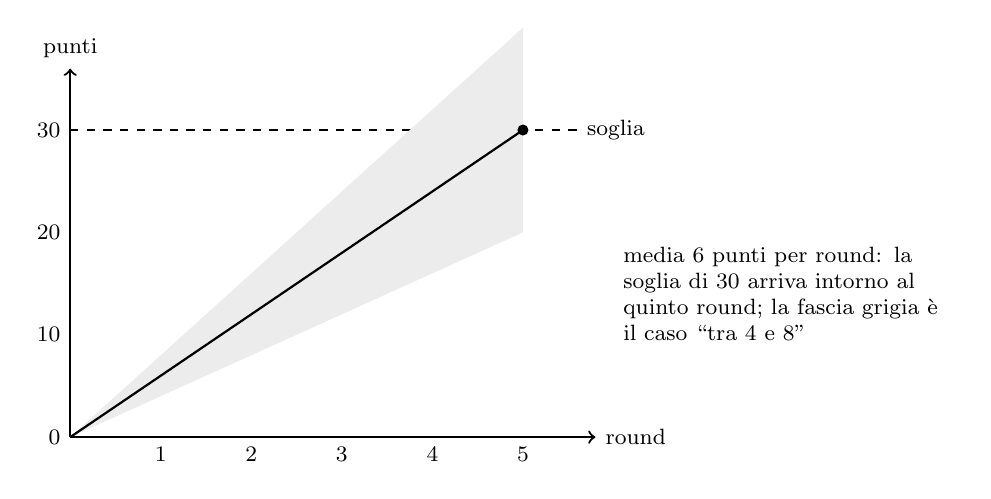
\begin{tikzpicture}[font=\small, x=1.15cm, y=0.13cm]
  \draw[thick, ->] (0,0) -- (5.8,0) node[right, font=\footnotesize] {round};
  \draw[thick, ->] (0,0) -- (0,36) node[above, font=\footnotesize] {punti};
  \foreach \x in {1,...,5} \node[below, font=\footnotesize] at (\x,0) {\x};
  \foreach \y in {0,10,20,30} \node[left, font=\footnotesize] at (0,\y) {\y};
  \draw[dashed] (0,30) -- (5.6,30) node[right, font=\footnotesize] {soglia};
  \fill[gray!15] (0,0) -- (1,4) -- (2,8) -- (3,12) -- (4,16) -- (5,20) -- (5,40) --
    (4,32) -- (3,24) -- (2,16) -- (1,8) -- cycle;
  \draw[thick] (0,0) -- (1,6) -- (2,12) -- (3,18) -- (4,24) -- (5,30);
  \fill (5,30) circle (2pt);
  \node[font=\footnotesize, text width=4.2cm, align=left, anchor=west] at (6.0,14)
    {media 6 punti per round: la soglia di 30 arriva intorno al quinto round; la fascia
    grigia è il caso ``tra 4 e 8''};
\end{tikzpicture}
\caption{Il bilanciamento di durata con una soglia di punti, nell'esempio di Marta su
\emph{Root}: dal numero di round desiderato si ricava quanti punti deve poter fare un
giocatore in un round, e da lì il valore di ogni elemento.}
\label{a14:fig:durata}
\end{figure}

\paragraph{Tagliare i turni iniziali.} Che cosa si può fare per limare la durata? Si possono
\textbf{tagliare i turni iniziali}, che molto spesso presentano \textbf{poche scelte
significative}. Marta non invita a farlo sempre, anzi, ``con molta parsimonia''. Tra addetti
ai lavori si parla di \textbf{bilanciamento di Kramer}\footnote{Così nella trascrizione (``tra
detti e lavori si chiama il bilanciamento di Kramer''). Il riferimento è probabilmente al
designer tedesco Wolfgang Kramer, ma il capitolo non ha trovato una fonte che usi questo nome
per la tecnica.}: si danno \textbf{risorse di partenza} ai giocatori, perché i primi turni non
siano impiegati a raccogliere risorse. Ha delle insidie: rende sicuramente il gioco più
focalizzato e più attento, ma intanto bisogna fare \textbf{un buon bilanciamento delle risorse
iniziali}; e, se le risorse date sono diverse tra i giocatori, bisogna capire se partire con
certe risorse dia \textbf{un vantaggio}. È una cosa da fare \textbf{solo quando è necessaria}.
Alcuni giochi beneficiano di un \textbf{turno iniziale semplice e guidato}, che è anche uno
degli \textbf{strumenti di approcciabilità}: è vero che quei turni si somigliano da una partita
all'altra, ma a volte servono ad agevolare l'ingresso nel gioco. Soprattutto in un gioco
pensato per andare oltre i confini del proprio genere, qualche turno semplice può aiutare le
persone a \textbf{entrare nel flusso}.

\paragraph{Tagliare i turni finali.} Si fa molto spesso negli \textbf{\emph{engine
building}}, i giochi a ``motore economico'', in cui c'è un \emph{feedback} che genera punti
vittoria o risorse, o che comunque avvicina alla condizione di fine partita. Il motore, andando
avanti, diventa sempre più performante; e se da un certo punto cresce in modo
\textbf{lineare o esponenziale}, diventa probabilmente impossibile per gli altri recuperare.
Allora si tagliano i turni finali: ``da questo punto in avanti è chiaro come andrebbe il resto
della partita, non c'è bisogno di giocarla'', per non tediare le altre persone. L'esempio è
\textbf{\emph{Race for the Galaxy}}: la partita finisce quando si esauriscono i
\textbf{gettoni punti} o quando qualcuno ha giocato \textbf{12 carte}. Di solito avviene quando
il motore si è innescato: i turni successivi ripeterebbero quello che si è già visto, perché
le strategie sono ormai impostate.

\paragraph{La durata dentro il turno.} Un'altra parola sulla durata \textbf{intraturno}. Se si
aggiungono tantissime \textbf{microscelte} dentro il turno, la persona si sentirà
\textbf{paralizzata} e spenderà molto tempo. E anche in una situazione normale, con poche
scelte, se per stare dietro a tutte le regole \textbf{vanno via 5 minuti}, quei 5 minuti vanno
\textbf{moltiplicati per il numero di persone e per il numero di round}: la durata di un gioco
cresce molto in fretta. E si stanno ancora omettendo le altre fasi, come quelle di
\textbf{amministrazione} o di \textbf{conteggio dei punti}. Bisogna quindi fare attenzione che
i turni non siano inutilmente lunghi; ma a volte \textbf{un turno lungo può essere molto
soddisfacente}. \emph{Root} dura, a detta di Marta, due ore e mezza, e i suoi turni sono molto
lunghi rispetto ad altri giochi simili; ma senza quei turni e senza quella durata il gioco ne
risentirebbe in termini di esperienza. ``Alla fine conta molto il gioco che stiamo facendo.''

\subsection{La domanda: come si calcola la durata sulla scatola?}

Uno studente chiede: sulle scatole c'è scritto quanto dura un gioco, ma spesso a lui sembra
\textbf{sottodimensionato}. Come viene calcolato? C'è uno standard?

``Lo standard in realtà non c'è'', risponde Marta. Tendenzialmente si dovrebbe indicare
\textbf{la durata media di una partita una volta che si conoscono le regole}. Quindi:
\begin{itemize}
  \item \textbf{non è mai compresa la spiegazione delle regole};
  \item \textbf{non è mai considerata la prima partita}: il valore vale più per chi ha giocato
        tre o quattro volte e conosce il gioco, e non è più al punto di riprendere in mano il
        regolamento.
\end{itemize}
Va da sé che il numero viene \textbf{sbagliato piuttosto spesso}, perché non è facile
stabilirlo. Il metodo migliore, secondo Marta, è prendere \textbf{il tempo medio del gruppo di
\emph{test} che conosce il gioco} e quello di chi fa \textbf{\emph{blind test}}, cioè di persone
alle prime armi, e vedere dove si assesta \textbf{il valore di mezzo}: non tutti giocheranno come
chi ha fatto cento partite, ma neanche ne faranno solo due; l'ideale sarebbe che a un gioco si
facessero \textbf{5--10 partite}. E poi dipende molto dai \textbf{gruppi di gioco}: non c'è un
vincolo su quanto si impiega a fare il proprio turno, e se si è al tavolo con persone che
pensano molto, le durate cresceranno. Si tende comunque a trovare una durata
\textbf{compatibile con il gioco}: un gioco per bambini non può durare due ore, ``ma queste
cose penso le intuite anche voi''.

\paragraph{Approfondimento: corto o lungo.} Schell dedica un intero tipo di bilanciamento
(``corto contro lungo'') alla durata: se il gioco è troppo corto, i giocatori non riescono a
sviluppare ed eseguire strategie significative; se è troppo lungo, si annoiano o lo evitano
per l'impegno di tempo. Le leve principali sono le condizioni di vittoria e di sconfitta. Due
suoi esempi mostrano soluzioni diverse dal taglio di turni: in \emph{Spy Hunter}, per i primi
novanta secondi il giocatore ha auto infinite, perché i principianti non abbiano partite
frustranti di pochi secondi; in \emph{Minotaur}, dopo venti minuti suona una campana e tutti i
sopravvissuti vengono trasportati in una stanza piena di mostri, così la partita finisce in
meno di venticinque minuti e c'è comunque un vincitore, lo stesso principio della zona che si
restringe nei \emph{battle royale}. È convergenza (sezione~\ref{a14:sec:difetti}) imposta per
regola.

% ---------------------------------------------------------------------
\section{Raddoppia o dividi la risorsa}
\label{a14:sec:raddoppia}

Un'altra tecnica ``molto popolare'' è \textbf{raddoppiare o dividere la risorsa}\footnote{Nella
trascrizione ``il raddoppio di vidi la risorsa''.}. A volte è importante capire \textbf{quanto
una risorsa incide sul gioco}, e dove ha senso bilanciarla, se farla crescere o diminuire: non
è sempre semplice capirlo. La tecnica base è: se c'è uno spazio azione dove si ottengono delle
risorse, \textbf{si raddoppia la quantità}, anche se il numero sembra grandissimo,
\textbf{oppure la si divide}. Raddoppiare o dividere è un'\textbf{estremizzazione}, ed
estremizzare una risorsa ne rende subito evidente l'impatto sul gioco: si applica la tecnica e
si vede come reagisce il sistema.

\paragraph{Le dipendenze.} Se la risorsa ha \textbf{tante dipendenze}, il sistema può
``fallire'': la modifica scombina tantissime cose a cascata, e la tecnica diventa praticamente
inutile, perché non restituisce alcun valore certo. Più dipendenze ha, più il rischio è alto.
Per esempio, è \textbf{poco rischioso} applicarla ai \textbf{punti vittoria}: raddoppiare o
dividere i punti di una carta specifica di solito ha poco impatto sul resto delle carte e dei
componenti, perché è \textbf{un valore finale}, con poche dipendenze. Va comunque valutato di
volta in volta.

\paragraph{Quanto deve pesare ogni parte.} Va considerato anche, come questione a sé,
\textbf{quanto valgono le varie parti del gioco}. Se si fa un gioco in cui si costruisce la
propria \textbf{città} sulla propria plancia, e poi ci sono \textbf{obiettivi} e
\textbf{risorse} che danno punti, e il \emph{focus} deve essere la città, allora la città deve
valere \textbf{il 50, 60, anche 70\%} del punteggio totale, riservando il \textbf{10--15\%}
agli altri sistemi che entrano nel conteggio finale. Non è un caso che in
\textbf{\emph{Wingspan}} \textbf{quasi il 50\%} dei punti derivi dalle \textbf{carte uccello} o
dall'uso di determinate abilità, perché sono il \emph{focus} del gioco: difficilmente si fa più
della metà dei punti con le risorse rimaste a fine partita o con le carte obiettivo. È anche una
questione di \textbf{dove mettere il \emph{focus} dell'esperienza}.

\paragraph{Una ricerca progressiva.} La tecnica può essere \textbf{progressiva}: applicando
costantemente il raddoppio o la divisione si arriva a trovare il \textbf{valore medio}. Si
continua a raddoppiare finché la risorsa non diventa \textbf{troppo incisiva}; da lì si torna
a dividere, cioè un po' indietro; e così, stringendo via via il campo, si trova il valore
giusto (figura~\ref{a14:fig:raddoppia}). Anche qui, però, bisogna capire se il valore
``giusto'' è quello che serve a \textbf{veicolare l'intento del \emph{design}}, o se è
semplicemente qualcosa che funziona ma finisce per \textbf{appiattire} il resto delle risorse:
``fare attenzione sempre al solito concetto''.

\begin{figure}[htbp]
\centering
\begin{tikzpicture}[font=\small, x=1.25cm, y=1cm]
  \draw[thick] (0,0) -- (9,0);
  \foreach \x/\l in {0.5/1, 1.5/2, 3.5/4, 7.5/8} {
    \draw (\x,-0.12) -- (\x,0.12);
    \node[below, font=\footnotesize] at (\x,-0.15) {\l};
  }
  \fill[gray!25] (3.5,-0.08) rectangle (7.5,0.08);
  \node[font=\footnotesize] at (5.5,-1.3) {qui sta il valore cercato};
  \draw[-{Stealth[length=2mm]}, thick] (0.5,0.3) to[bend left=40] node[above,
    font=\scriptsize] {$\times 2$} (1.5,0.3);
  \draw[-{Stealth[length=2mm]}, thick] (1.5,0.3) to[bend left=40] node[above,
    font=\scriptsize] {$\times 2$} (3.5,0.3);
  \draw[-{Stealth[length=2mm]}, thick] (3.5,0.3) to[bend left=40] node[above,
    font=\scriptsize] {$\times 2$: troppo!} (7.5,0.3);
  \draw[-{Stealth[length=2mm]}, thick] (7.5,-0.2) to[bend left=40] node[below,
    font=\scriptsize] {a metà strada} (5.5,-0.2);
  \node[font=\footnotesize, text width=4.3cm, align=left, anchor=west] at (9.2,0.2)
    {1: poco incisiva\\ 2, 4: ancora poco\\ 8: troppo incisiva\\ $\Rightarrow$ si torna
    indietro e si stringe tra 4 e 8};
\end{tikzpicture}
\caption{Raddoppia o dividi come ricerca progressiva: si estremizza la risorsa finché il suo
impatto non diventa evidente, poi si torna indietro stringendo l'intervallo. Funziona bene su
valori con poche dipendenze, come i punti vittoria di una carta.}
\label{a14:fig:raddoppia}
\end{figure}

\paragraph{Approfondimento: la regola di Sid Meier.} Schell riporta la stessa tecnica come
``regola del raddoppio e del dimezzamento'': quando si cambia un valore per bilanciare, si
spreca tempo a cambiarlo di poco; conviene raddoppiarlo o dimezzarlo nella direzione in cui
deve andare, e poi, se si è esagerato, provare a metà strada. L'esempio è un razzo che fa 100
punti di danno: se sembrano troppi, non si scende a 90 o 80, ma a 50. La regola è spesso
attribuita a Brian Reynolds, che però, interpellato da Schell, ne dà il merito a \textbf{Sid
Meier}: lo prese da parte, all'inizio degli anni Novanta, mentre lavoravano a
\emph{Colonization}, dopo averlo visto cambiare ripetutamente un valore del 10\%. Il punto,
dice Reynolds, è cambiare qualcosa in modo da \emph{sentire} subito la differenza, invece di
perdersi a chiedersi se si è avuto un effetto, o peggio vederne uno che non c'è, magari per
una serie sfortunata di numeri casuali.

% ---------------------------------------------------------------------
\section{Due problemi, una soluzione}
\label{a14:sec:dueproblemi}

Un'altra tecnica molto usata, soprattutto \textbf{all'inizio dello sviluppo}: \textbf{due
problemi, una soluzione}. Quando si trova un problema, \textbf{non lo si risolve subito}: se ne
cerca \textbf{almeno un altro}, e si applica \textbf{una soluzione a entrambi}, cioè una sola
modifica che li risolva tutti e due. Questo aiuta a \textbf{far convergere il lavoro}, verso
una riduzione del numero di problemi: magari la soluzione ne fa emergere un altro, ma
generalmente \textbf{non ne fa emergere altri due}, e così si progredisce.

È utile all'inizio. Applicata \textbf{verso la fine}, ci si accorge che intanto è \textbf{poco
efficace}, e soprattutto che la soluzione trovata \textbf{impatta molto più forte} su tutti gli
altri sistemi. Il consiglio è di usarla principalmente all'inizio, e di fare attenzione
\textbf{all'impatto di ciascuna leva}: risolvendo due problemi con una nuova soluzione si
modificano leve che a loro volta possono creare problemi. Purtroppo questo si risolve solo in
due modi: con \textbf{l'esperienza}, cioè sapendo più o meno che cosa succede quando si
applicano certe soluzioni, e con i \textbf{\emph{test}}, perché a volte non c'è modo di
risolvere i problemi se non empiricamente.

% ---------------------------------------------------------------------
\section{Gli elementi ricorrenti del bilanciamento}
\label{a14:sec:elementi}

Seguono ``vari elementi'' che ricorrono quando si parla di bilanciamento e di sviluppo, e per
cui Marta non ha trovato ``un modo coerente di metterli'': in questa slide ha cercato di
trasmettere ``quelle cose che si apprendono un po' per esperienza''. La
tabella~\ref{a14:tab:elementi}, alla fine della sezione, li riassume.

\subsection{Le progressioni di punteggio}

Ci sono \textbf{progressioni note} per i punteggi. Una classica è \textbf{1, 3, 6, 10, 15}: tra
un numero e l'altro l'incremento cresce di uno (+2, +3, +4, +5). Serve, per esempio, in una
\textbf{collezione di set}, a rendere la collezione \textbf{sempre più premiante} man mano che
cresce. Una progressione ancora più forte è quella \textbf{quadratica}: con 5 pezzi di una
risorsa si fanno \textbf{25 punti}; cresce molto più rapidamente dell'altra, e quindi si dà
\textbf{ancora più importanza} a quella risorsa. Oppure ci può essere una progressione
\textbf{penalizzante}: dà punti fino a un certo punto, per esempio 1, 3, 6, e poi
\textbf{scende}, 5, 4; dice che quella risorsa la si vuole, \textbf{``ma non troppo''}
(figura~\ref{a14:fig:progressioni}).

Sono elementi che tornano comodi quando si ha una collezione di set e si vuole creare una certa
esperienza in linea con il \emph{design}. Molto spesso la prima cosa che si fa è prendere una
di queste progressioni ``classiche'', applicarla e vedere come reagisce il gioco; ``in rari casi
vengono cambiate''.

\begin{figure}[htbp]
\centering
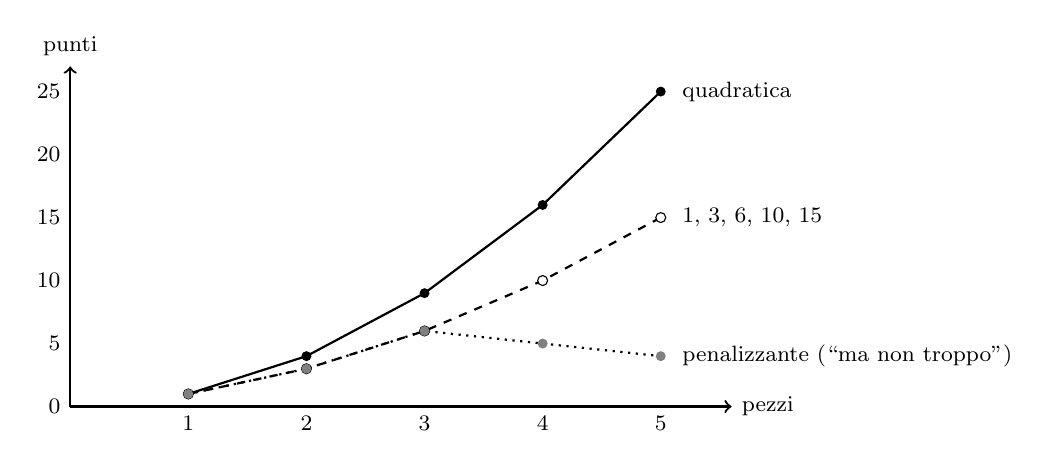
\begin{tikzpicture}[font=\small, x=1.5cm, y=0.16cm]
  \draw[thick, ->] (0,0) -- (5.6,0) node[right, font=\footnotesize] {pezzi};
  \draw[thick, ->] (0,0) -- (0,27) node[above, font=\footnotesize] {punti};
  \foreach \x in {1,...,5} \node[below, font=\footnotesize] at (\x,0) {\x};
  \foreach \y in {0,5,10,15,20,25} \node[left, font=\footnotesize] at (0,\y) {\y};
  % quadratica
  \draw[thick] (1,1) -- (2,4) -- (3,9) -- (4,16) -- (5,25);
  \foreach \x/\y in {1/1,2/4,3/9,4/16,5/25} \fill (\x,\y) circle (1.8pt);
  \node[font=\footnotesize, anchor=west] at (5.1,25) {quadratica};
  % triangolare
  \draw[thick, dashed] (1,1) -- (2,3) -- (3,6) -- (4,10) -- (5,15);
  \foreach \x/\y in {1/1,2/3,3/6,4/10,5/15} \fill[white, draw=black] (\x,\y) circle (1.8pt);
  \node[font=\footnotesize, anchor=west] at (5.1,15) {1, 3, 6, 10, 15};
  % penalizzante
  \draw[thick, dotted] (1,1) -- (2,3) -- (3,6) -- (4,5) -- (5,4);
  \foreach \x/\y in {1/1,2/3,3/6,4/5,5/4} \fill[gray] (\x,\y) circle (1.8pt);
  \node[font=\footnotesize, anchor=west] at (5.1,4) {penalizzante (``ma non troppo'')};
\end{tikzpicture}
\caption{Le tre progressioni di punteggio di cui parla Marta. Più ripida è la curva, più il
gioco spinge a concentrarsi su quella collezione; una curva che scende dopo un massimo dice
che la risorsa serve, ma non in eccesso.}
\label{a14:fig:progressioni}
\end{figure}

\subsection{Mettere in relazione le risorse: moltiplicazioni e set}

\paragraph{La moltiplicazione.} Si possono \textbf{mettere in relazione due risorse}, per
esempio con una \textbf{moltiplicazione}: si ottengono punti pari a \textbf{risorsa A per risorsa
B}. L'intento di sviluppo che questo veicola è che si vogliono \textbf{possibilmente tante A
quante B}, e non tante dell'una e poche dell'altra: per come funziona la moltiplicazione, a
parità di pezzi totali si ottiene di più se i due numeri sono uguali che se uno è molto alto e
l'altro molto basso (con 6 pezzi, $3 \times 3 = 9$, mentre $5 \times 1 = 5$). È una cosa che si
adotta quando si vede che c'è \textbf{troppa concentrazione su una delle due risorse}, magari
perché risulta più premiante: la moltiplicazione le \textbf{ribilancia}, in modo che abbiano lo
stesso interesse.

\paragraph{Il set.} Lo stesso vale per più di due risorse, tre o quattro, quando si vuole che
nel gioco \textbf{siano tutte importanti} e non vengano trascurate: allora si premia
\textbf{il set}. Per ogni set completo, cioè almeno una di ciascuna risorsa, si dà un certo
punteggio.

\paragraph{Punteggio verticale e orizzontale.} Marta non ricorda il termine inglese di
partenza (``mi sfugge il termine'') e li chiama \textbf{punteggio verticale} e
\textbf{punteggio orizzontale}. Il \textbf{verticale} è quello classico: questa risorsa dà
tanto, quest'altra tanto, per quello che ho ottenuto nel gioco. L'\textbf{orizzontale} prende
\textbf{l'altro asse}, e analizza \textbf{quante risorse diverse} ho ottenuto: è il caso, molto
spesso, del calcolo dei set di risorse.

``Anche queste sono tutte cose che trovate standard.'' Ed è anche per questo, come diceva la
volta precedente, che è importante \textbf{giocare tanti giochi}, conoscere tanto, avere
curiosità, esplorare anche giochi \textbf{fuori dalla propria \emph{comfort zone}} e
guardarli con occhio critico: ci si accorge che molte di queste cose sono riusate in
tantissimi giochi.

\subsection{L'esclusività delle risorse}

Si torna all'esempio di \emph{Splendor}: c'è un motivo per cui lì le risorse sono
\textbf{esclusive}, cioè i gettoni sono \textbf{in numero prefissato}. ``Mi sembra che sono
10, ora non sono sicurissima''\footnote{Nel gioco i gettoni gemma sono 7 per colore, più 5
gettoni oro jolly, e se ne usano meno con due o tre giocatori. Il numero esatto non cambia il
ragionamento di Marta.}, per ogni risorsa, e le persone ne possono prendere \textbf{tre a turno}
con la propria azione. Essendo esclusive, il gioco si basa anche sulla \textbf{scarsità}: è una
strategia lecita \textbf{prendere delle risorse per toglierle} agli altri e fare in modo che
non ci siano per le altre persone al tavolo. E l'effetto si propaga: se c'è una carta che
interessa a più giocatori, togliendo la risorsa dal tavolo la carta diventa \textbf{esclusiva a
sua volta}, perché nessun altro la può completare. Poi la cosa si manifesta come un aspetto di
\textbf{\emph{timing}}: diventa importante \textbf{quando} restituire quelle risorse.

\paragraph{Da limite a opportunità.} Marta lo dice perché molto spesso l'esclusività delle
risorse è nata come \textbf{limite}, per via del \textbf{numero di componenti}: essendo un
prodotto fisico, come visto parlando dei limiti della componentistica, è complicato mettere
tante cose in una scatola. Ma, come tutti i limiti, a un certo punto è diventata
un'\textbf{opportunità} di \emph{design} e di sviluppo: quando ci si accorge che c'è
\textbf{poca interazione tra i giocatori}, introdurre l'esclusività delle risorse a volte fa
esattamente quello che serve per \textbf{generare interazione}. Lo stesso vale per gli
\textbf{incentivi}, sia nel restituire queste risorse sia nel prenderle, nel caso la risorsa
sia esclusiva ma i giocatori non la prendano in considerazione.

\subsection{La crescita tra i round}

Un altro aspetto importante è la \textbf{crescita tra round}. In molti giochi è importante che
tra un round e l'altro \textbf{ci sia una differenza}: se in tutti i round si ha accesso alle
stesse identiche risorse, la stessa situazione sulla plancia, le stesse possibilità, il gioco
risulta \textbf{statico}. La crescita fa percepire \textbf{la progressione} a chi gioca. A volte
viene tralasciata, ma si può fare in modo abbastanza semplice: se c'è una \textbf{rendita}, la
rendita cresce; oppure, man mano che si piazzano cose sul tabellone, si \textbf{sbloccano} cose
sulla propria plancia che danno più possibilità andando avanti. È un elemento che nello
sviluppo viene esaminato molto spesso, perché magari il gioco funziona, ma ha \textbf{una
crescita piatta}, e bisogna lavorare per farla aumentare.

\subsection{Il controllo dell'alea e del caos}

Altro elemento frequente: il \textbf{controllo dell'alea o del caos}. Il gioco può presentare
sia alea sia caos, ma in modo \textbf{estremizzato}, e allora bisogna trovare strumenti per
regolarli. L'esempio più classico: \textbf{lancio un dado e spendo una risorsa per fare il
\emph{re-roll}}. Molti giochi con questa meccanica non avevano di base il \emph{re-roll}: è
stato aggiunto \textbf{in fase di sviluppo}, perché si è visto che il lancio di dado senza
possibilità di rilancio è un'esperienza \textbf{frustrante} per la maggior parte di chi gioca.
C'è poi l'esempio pratico di \textbf{\emph{Magical Athlete}}, che ha ``abbattuto un po' questa
concezione'': oggi ci sono giochi che accettano ``un po' più di buon grado'' anche il lancio
del dado senza controllo. Ma in fase di sviluppo questo resta uno degli elementi su cui si va a
incidere. Un altro esempio: tessere pescate \textbf{da un sacchetto}, con la possibilità di
\textbf{pescarne più di una}, o di \textbf{rimettere} quella pescata e pescarne un'altra.

\subsection{Le probabilità}

È utile avere \textbf{una base di probabilità}. L'esempio più classico è il dado, e sapere come
usare i dadi in un gioco ``può fare la differenza''.

\paragraph{Lineare.} Un dado da 1 a 6 ha una probabilità cosiddetta \textbf{lineare}
(uniforme): ogni faccia ha la stessa probabilità di uscire.

\paragraph{A campana.} Con \textbf{due dadi} la probabilità segue una \textbf{curva a campana}:
il risultato medio è più probabile dei risultati agli estremi. ``Penso che questo lo sappiate'':
con due dadi è molto più probabile fare \textbf{7} che fare 2 o 12. È una particolarità che può
\textbf{informare le decisioni}. Si immagini un \textbf{gioco di percorso} in cui si lancia un
solo dado: si dà la stessa probabilità a tutte le facce, e mediamente ci si muove di
\textbf{3,5}, il valore medio di un dado. Con due dadi, invece, uscirà più spesso il 7: è un
sistema ``più morbido'', perché i risultati estremi sono più rari. Con un dado solo, il 6 può
uscire tanto quanto il 3 o il 4, e solo su molti lanci la media si riporta a 3,5. Questo aiuta
a capire che cosa serve in funzione del gioco (figura~\ref{a14:fig:dadi}).

\paragraph{Calante.} La probabilità può anche essere \textbf{calante}. Si immagini di poter
scegliere quante risorse ottenere, \textbf{da una a cinque}, ma per ogni risorsa voluta bisogna
\textbf{lanciare una moneta}. Se se ne prende una, si lancia una moneta: con testa la si tiene,
con croce no. Se se ne vogliono cinque, si lanciano cinque monete, ma \textbf{basta una sola
croce per non tenerne nessuna}. La probabilità \textbf{cala} al crescere delle risorse che si
vogliono ottenere. Si usa anche questo: per esempio, in un gioco di percorso, ``posso muovermi
di quanto mi pare, ma poi lancio il dado'', e se il risultato è inferiore allo spostamento
dichiarato devo tornare indietro, o non mi muovo affatto.

Sono piccoli meccanismi che influenzano e guidano le scelte, e che aiutano a regolare lo
sviluppo: magari in fase di \emph{design} si è detto ``mi interessa che sia un gioco di
percorso, mi basta lanciare un dado da 6 e andare dove vado''; ma in sviluppo si vuole che la
decisione sia \textbf{più controllata}, e si possono inserire strutture come il
\textbf{cambiare la probabilità} di quel meccanismo.

\begin{figure}[htbp]
\centering
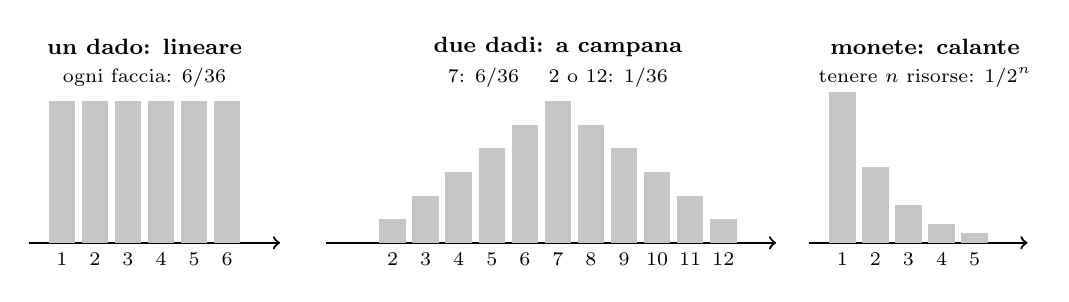
\begin{tikzpicture}[font=\small, x=0.42cm, y=0.30cm]
  % un dado
  \node[font=\footnotesize\bfseries] at (3.5,8.3) {un dado: lineare};
  \draw[thick, ->] (0,0) -- (7.6,0);
  \foreach \v in {1,...,6} {
    \fill[gray!45] (\v-0.4,0) rectangle (\v+0.4,6);
    \node[below, font=\scriptsize] at (\v,0) {\v};
  }
  \node[font=\scriptsize] at (3.5,7.0) {ogni faccia: 6/36};
  % due dadi
  \begin{scope}[shift={(9,0)}]
    \node[font=\footnotesize\bfseries] at (7,8.3) {due dadi: a campana};
    \draw[thick, ->] (0,0) -- (13.6,0);
    \foreach \v/\h in {2/1,3/2,4/3,5/4,6/5,7/6,8/5,9/4,10/3,11/2,12/1} {
      \fill[gray!45] (\v-0.4,0) rectangle (\v+0.4,\h);
      \node[below, font=\scriptsize] at (\v,0) {\v};
    }
    \node[font=\scriptsize] at (7,7.0) {7: 6/36 \quad 2 o 12: 1/36};
  \end{scope}
  % monete
  \begin{scope}[shift={(23.6,0)}]
    \node[font=\footnotesize\bfseries, align=center] at (3.5,8.3) {monete: calante};
    \draw[thick, ->] (0,0) -- (6.6,0);
    \foreach \v/\h in {1/6.4,2/3.2,3/1.6,4/0.8,5/0.4} {
      \fill[gray!45] (\v-0.4,0) rectangle (\v+0.4,\h);
      \node[below, font=\scriptsize] at (\v,0) {\v};
    }
    \node[font=\scriptsize, align=center] at (3.5,7.0) {tenere $n$ risorse: $1/2^n$};
  \end{scope}
\end{tikzpicture}
\caption{Le tre forme di probabilità dell'esempio di Marta: il dado singolo (ogni faccia
ugualmente probabile, media 3,5), due dadi (il 7 è sei volte più probabile del 2 o del 12) e la
probabilità calante delle monete (per tenere $n$ risorse servono $n$ teste di fila: 50\%,
25\%, 12,5\%\ldots). Le barre sono in scala all'interno di ciascun grafico.}
\label{a14:fig:dadi}
\end{figure}

\begin{table}[htbp]
\centering
\small
\begin{tabular}{@{}p{3.2cm}p{5.2cm}p{5.0cm}@{}}
\toprule
\textbf{Tecnica o elemento} & \textbf{Che cosa fa} & \textbf{Attenzione a} \\
\midrule
Budget di complessità & ciò che si toglie libera complessità, da eliminare o reinvestire
  nel \emph{focus} & nel dubbio, meglio accessibile \\
\addlinespace
Alto e basso rischio & crea una scelta sensibile con due macro-strategie comunicanti & la
  ricompensa deve valere il rischio \\
\addlinespace
Ancoraggio & tutto è rapportato a un valore ancora (\emph{Stone Age}: un puntino = un punto)
  & risorse interdipendenti, turni extra, \emph{draft} \\
\addlinespace
Durata & round o soglie fissate $\Rightarrow$ punti per round $\Rightarrow$ valore dei
  pezzi; tagliare turni iniziali o finali & la durata intraturno si moltiplica per persone
  e round \\
\addlinespace
Raddoppia o dividi & estremizza per vedere l'impatto, poi stringe & le dipendenze; il
  valore ``giusto'' può appiattire \\
\addlinespace
Due problemi, una soluzione & fa convergere il lavoro & solo all'inizio dello sviluppo \\
\addlinespace
Progressioni & 1-3-6-10-15, quadratica, penalizzante & che cosa si vuole premiare \\
\addlinespace
$A \times B$ e set & spingono a bilanciare le risorse tra loro & punteggio verticale contro
  orizzontale \\
\addlinespace
Esclusività & scarsità, interazione, \emph{timing} & nata come limite di componenti \\
\addlinespace
Crescita tra round & progressione percepita (rendite, sblocchi) & la crescita piatta \\
\addlinespace
Controllo dell'alea & \emph{re-roll}, più pescate, rimettere nel sacchetto & non sempre serve
  (\emph{Magical Athlete}) \\
\addlinespace
Probabilità & lineare, a campana, calante & scegliere la forma che serve all'esperienza \\
\bottomrule
\end{tabular}
\caption{Gli strumenti di bilanciamento presentati nella lezione, nell'ordine in cui li
presenta Marta.}
\label{a14:tab:elementi}
\end{table}

\paragraph{Approfondimento: la probabilità per chi progetta.} Schell dedica un capitolo alla
probabilità con dieci ``regole'', e una delle sue osservazioni conferma il consiglio di Marta
di testare invece di calcolare: il \emph{metodo Monte Carlo}, cioè ripetere la prova molte volte
e contare i risultati, ``a volte dà risultati più utili della probabilità teorica, perché è una
misura della cosa reale''. La sua ultima regola, scherzosa, è la più pratica: quando un calcolo
si fa difficile, cercare qualcuno che si consideri ``un mago della matematica'', che ne sarà
entusiasta. Brathwaite e Schreiber, in \emph{Challenges for Game Designers}, dedicano invece un
intero capitolo all'equilibrio tra caso e abilità, il tema del controllo dell'alea.

% ---------------------------------------------------------------------
\section{Smussare la stella}
\label{a14:sec:stella}

``Vediamo, ok. Forse devo correre un po', allora.'' \textbf{Non è detto che chi crea il gioco
abbia chiaro il \emph{design}.} Per spiegarlo Marta usa un modo di dire: un gioco è
\textbf{una stella}, e lo sviluppo \textbf{smussa gli angoli}, perché le punte non blocchino
l'ingresso in un ipotetico buco (``non so come dirlo meglio''). Le punte rappresentano le
\textbf{qualità e le particolarità del \emph{design}}. Come detto la volta prima, il
\emph{design} è anche \textbf{personale} e dovrebbe sfuggire un po' alle logiche di mercato; e
così anche lo sviluppo. Oggi tenere alcune punte è diventato più importante che in passato;
tuttavia si smussa, perché \textbf{più punte ha la stella, meno è digeribile per un pubblico
ampio}: le persone hanno bisogno di un po' di \textbf{familiarità} e di un po' di
\textbf{novità}, non accettano una cosa totalmente innovativa, ma neanche ne vogliono una
estremamente familiare. È un gioco di \textbf{trovare il punto giusto}.

\paragraph{Chi ha creato il gioco può non vedere l'intento.} In questo, a volte, anche chi ha
creato il gioco ha poco chiaro l'intento del \emph{design}, nonostante il gioco lo manifesti:
viene fuori giocandolo. Lo sviluppo deve però evitare di \textbf{finire sui \emph{bias}
personali}: se si ha un genere preferito, bisogna fare attenzione a non mettere la propria
preferenza in tutti i giochi. Se si fa un gioco per bambini, è inutile metterci le dinamiche di
un \textbf{motore economico}: ``non funziona'', o quanto meno sarà molto complicato far capire a
un bambino come funziona economicamente un motore di gioco. ``So che sembra una banalità'', ma è
una tendenza in cui si cade con estrema facilità, anche in casi che sembrano estremi.

\paragraph{Il GCD come bussola.} Il \textbf{\emph{Game Concept Document}} dà il \emph{focus} per
restare sul progetto: averlo sempre a portata di mano aiuta a ricordare che cosa si sta
facendo, come lo si sta facendo, e \textbf{che cosa si può davvero smussare} senza intaccare
uno dei \textbf{pilastri}, cosa che comprometterebbe davvero il \emph{design}. Resta il fatto che
\textbf{se una cosa non è fondamentale all'esperienza, può essere tolta}.

\paragraph{Ma attenzione a che cosa è ``fondamentale''.} La valutazione personale porta sempre
il rischio di sbagliarsi. Una cosa che \textbf{sembra} non fondamentale, come i \textbf{testi di
ambientazione} (\emph{flavor text}) su alcune carte, solo perché non entrano in gioco in modo
meccanico, a volte viene considerata non incisiva. Ma se \textbf{\emph{Wingspan}} non avesse i
testini che raccontano i comportamenti degli uccelli e tutto il resto, probabilmente non avrebbe
la stessa potenza, la stessa capacità di fare leva su tantissime persone che ha avuto nella
pratica. Alcune cose non sembrano fondamentali, ``ma fanno la differenza''.

\paragraph{Approfondimento: l'eleganza e il dettaglio.} Schell elenca tra i dodici tipi di
bilanciamento anche ``semplice contro complesso'' e ``dettaglio contro immaginazione'', e
propone una \emph{lente dell'eleganza}: un sistema elegante fa molto con pochi elementi. Ma per
lui l'eleganza non è il taglio indiscriminato: i dettagli che \emph{nutrono} l'immaginazione,
e che l'immaginazione può riusare più e più volte, vanno tenuti. I testi di \emph{Wingspan} sono
esattamente questo tipo di dettaglio.

% ---------------------------------------------------------------------
\section{I ``difetti'' dei giochi da tavolo}
\label{a14:sec:difetti}

``Ok, vediamo alcuni dei difetti cosiddetti dei giochi da tavolo.'' Le virgolette sono volute:
molte di queste cose vengono elencate come difetti, \textbf{ma non lo sono}. Lo sono se sono
\textbf{una dinamica che va contro l'esperienza attesa}: ``tendenzialmente sì, se va contro
l'esperienza attesa, di fatto lo possiamo chiamare difetto''. Ma \textbf{non esistono meccaniche
che siano difetti a priori}: vanno viste in funzione del gioco. Molto spesso le persone
confondono le meccaniche che generano \textbf{stati d'animo negativi} (la
\textbf{frustrazione}, a volte la \textbf{noia}) con difetti del gioco. Non è sempre così.
\textbf{Attenzione ai \emph{feedback}}, quindi: molto spesso vi elencheranno queste cose come
difetti, e non è detto che lo siano. Una slide lo riassume: bisogna distinguere
\textbf{l'intento del \emph{design}} dalle \textbf{dinamiche incontrollate}. Il ``difetto'' era
un intento del \emph{design}, oppure è lì perché è un \textbf{aspetto vestigiale del genere}, e
genera dinamiche che neanche il designer sa controllare? La tabella~\ref{a14:tab:difetti} li
riassume.

\paragraph{L'eliminazione dei giocatori: \emph{Bang!}.} La \textbf{\emph{player elimination}}
viene prima perché probabilmente la conoscono tutti, per via di \textbf{\emph{Bang!}}. Tantissime
persone si lamentano di \emph{Bang!} perché c'è l'eliminazione dei giocatori, ma poche si
rendono conto che \textbf{\emph{Bang!} senza eliminazione non funzionerebbe}: sarebbe un gioco
poco efficace. L'eliminazione garantisce che \textbf{tutta la partita sia giocata in tensione};
che non si possano \textbf{scaricare le risorse} liberamente senza pensarci, perché poi si
giocherebbe tutta la partita senza risorse; e fa tutta la differenza sulle
\textbf{ritorsioni}: in certi casi ``posso permettermi di finire le risorse perché so che non
subirò ritorsioni'', cosa che senza eliminazione non sarebbe possibile. La narrativa sottesa di
\emph{Bang!}, e il motivo per cui continua a piacere a tantissime persone, è legata anche
all'eliminazione: è un gioco sul \textbf{Far West}, in un certo senso spietato, che vuole
trasmettere una narrativa con \textbf{\emph{high stakes}}, una posta in gioco
altissima\footnote{Marta dice ``delle \emph{high stakes}, delle alte\ldots{} non mi torna il
termine italiano, perdonatemi''.}. Ci sono però giochi in cui l'eliminazione è \textbf{poco
giustificata}: in un gioco in cui si coopera per salvare il pianeta, ha poco senso eliminare
un giocatore a caso, ``adesso faccio per dire; poi magari trovate la chiave di lettura per cui
ha senso''.

\paragraph{\emph{Runaway leader} e \emph{bash the leader}: \emph{Root}.} Anche queste sono
spesso viste come negative. Il \textbf{\emph{runaway leader}} è quando un giocatore prende un
distacco tale che diventa difficile recuperarlo. La dinamica contrapposta è il \textbf{\emph{bash
the leader}}\footnote{Nella trascrizione ``Base the Leader'' e ``best dei leader''.}: le persone
individuano chi potrebbe ``correre via'' e vincere, e lo \textbf{bastonano}, letteralmente;
tutti se la prendono con la stessa persona, quella in testa. Entrambe possono essere utili in
giochi che rappresentano \textbf{dinamiche di potere}. \emph{Root}, che rappresenta proprio le
dinamiche di potere tra fazioni diverse, ha fatto del \emph{bash the leader} una delle sue
caratteristiche peculiari: il designer l'ha voluta mettere dentro con l'obiettivo di far
ruotare il gioco attorno a questa cosa. Non è una dinamica non voluta: è
\textbf{desiderata}, e il gioco dà gli strumenti sia per metterla in pratica sia per evitare che
diventi incontrastabile.

\paragraph{I \emph{feedback loop}.} Sono quando le risorse o i meccanismi di gioco
\textbf{informano la decisione successiva}. Un \emph{feedback loop} \textbf{positivo}: spendo
risorse e ottengo punti vittoria, e magari un'altra risorsa, che posso usare per ottenere altri
punti e altre risorse: ``capite che cresce all'infinito''. Un \emph{feedback loop}
\textbf{negativo}: eseguire qualcosa non dà qualcosa che rinforza il ciclo, e quindi rifarlo non
è premiante, e questo smorza le fasi successive. Sono dinamiche da tenere d'occhio, perché
possono compromettere l'intento.

\paragraph{Il \emph{kingmaking}.} ``Il \emph{kingmaking} è un'altra\ldots{} vabbè'': Marta non si
dilunga, ``se avete qualche curiosità''\footnote{Il \emph{kingmaking} è la situazione in cui
un giocatore che non può più vincere decide, con le sue mosse, chi tra gli altri vincerà.}.

\paragraph{Divergenza e convergenza.} Le trova ``sempre interessanti''. Molto spesso i giochi
\textbf{non convergono}, cioè non arrivano a una fine: il \emph{design} magari è bello, ma chi
l'ha creato \textbf{non ha pensato a come finisce}, e il gioco può \textbf{stallare}, non
concludersi mai. Bisogna sapere come farlo convergere, e ci sono meccanismi per farlo. Se la
fine del gioco è legata alla \textbf{fine del mazzo}, in un gioco in cui le carte vengono
\textbf{rimesse nel mazzo}, c'è \textbf{divergenza}: il gioco potrebbe non finire mai, perché il
mazzo non finisce mai. Se invece le carte pescate \textbf{non vengono reinserite} in nessun modo
e ogni turno se ne devono pescare \textbf{due}, si sa che \textbf{entro $n/2$ turni la partita
sarà finita}, con $n$ carte nel mazzo (figura~\ref{a14:fig:convergenza}). ``Vedete, questi
valori un po' così, perché è un po' diverso il valore vero; tuttavia fate finta che ora vada
bene''\footnote{La precisazione di Marta è giusta: se a pescare sono più giocatori, o se ci sono
altri modi di consumare il mazzo, il conto cambia. Il principio, cioè che una risorsa che si
consuma senza tornare indietro garantisce la fine, resta.}.

\begin{figure}[htbp]
\centering
\begin{tikzpicture}[
  font=\small,
  a14b/.style={draw, thick, rounded corners=3pt, text width=2.0cm, align=center,
               minimum height=0.9cm, fill=white},
  a14arr/.style={-{Stealth[length=2.5mm]}, thick}
]
  \node[font=\footnotesize\bfseries] at (2.0,1.6) {divergente};
  \node[a14b] (m1) at (0,0) {mazzo};
  \node[a14b] (g1) at (4,0) {gioco};
  \draw[a14arr] (m1.north east) to[bend left=25] node[above, font=\footnotesize] {pesca}
    (g1.north west);
  \draw[a14arr] (g1.south west) to[bend left=25] node[below, font=\footnotesize]
    {rimetti nel mazzo} (m1.south east);
  \node[font=\footnotesize, text width=4.6cm, align=center] at (2.0,-1.75) {il mazzo non
    finisce mai: la partita può stallare};
  \node[font=\footnotesize\bfseries] at (9.0,1.6) {convergente};
  \node[a14b] (m2) at (7,0) {mazzo da $n$ carte};
  \node[a14b] (g2) at (11,0) {scarti};
  \draw[a14arr] (m2) -- node[above, font=\footnotesize] {2 a turno} (g2);
  \node[font=\footnotesize, text width=4.6cm, align=center] at (9.0,-1.75) {niente torna
    indietro: entro circa $n/2$ turni la partita finisce};
\end{tikzpicture}
\caption{Divergenza e convergenza nell'esempio di Marta: legare la fine della partita alla fine
di un mazzo funziona solo se il mazzo si consuma davvero.}
\label{a14:fig:convergenza}
\end{figure}

\paragraph{L'ordine di turno.} Infine, attenzione all'\textbf{ordine di turno}: come sono
disposti i giocatori può \textbf{influenzare la partita di chi segue}, e il \textbf{primo
giocatore} potrebbe avere dei vantaggi. Anche \textbf{come sono distribuite le risorse
iniziali} tra i giocatori va guardato con attenzione. L'esempio classico è fare una serie di
\emph{test} attenti proprio a questo: se faccio iniziare sempre la stessa persona e questa
vince sistematicamente, da qualche parte c'è un problema. Questo è uno di quei casi che
``raramente può non essere un difetto: tendenzialmente lo è''. Ma anche qui c'è un'eccezione:
in un gioco che vuole mostrare \textbf{meccanismi di potere diversi}, il primo giocatore può
essere avvantaggiato di proposito. Marta pensa a \textbf{\emph{Il Grande Dalmuti}}, in cui il
Grande Dalmuti, che comincia a giocare, è avvantaggiato: ma quello è un gioco che vuole proprio
far percepire \textbf{la differenza di potere} tra i giocatori al tavolo\footnote{\emph{Il Grande
Dalmuti} è anch'esso di Richard Garfield (1995).}.

\begin{table}[htbp]
\centering
\small
\begin{tabular}{@{}p{3.0cm}p{4.8cm}p{5.6cm}@{}}
\toprule
\textbf{``Difetto''} & \textbf{Che cos'è} & \textbf{Quando è voluto (esempio di Marta)} \\
\midrule
\emph{Player elimination} & un giocatore esce dalla partita & \emph{Bang!}: tensione, niente
  risorse sprecate, ritorsioni, narrativa del Far West \\
\addlinespace
\emph{Runaway leader} & un distacco irrecuperabile & in giochi sulle dinamiche di potere \\
\addlinespace
\emph{Bash the leader} & tutti contro chi è in testa & \emph{Root}: il gioco ruota attorno a
  questo, e dà strumenti per farlo e per evitarlo \\
\addlinespace
\emph{Feedback loop} & positivo: cresce all'infinito; negativo: rifare non premia & da tenere
  d'occhio rispetto all'intento \\
\addlinespace
\emph{Kingmaking} & chi non può vincere decide chi vince & (non approfondito) \\
\addlinespace
Divergenza & il gioco non converge, stalla & mai: va fatto convergere \\
\addlinespace
Ordine di turno & chi inizia vince sistematicamente & raramente: \emph{Il Grande Dalmuti}, che
  vuole far sentire la differenza di potere \\
\bottomrule
\end{tabular}
\caption{I ``difetti'' dei giochi da tavolo: dinamiche che diventano difetti solo se vanno
contro l'esperienza attesa. La domanda è sempre se siano intento del \emph{design} o dinamiche
incontrollate, magari vestigia del genere.}
\label{a14:tab:difetti}
\end{table}

\paragraph{Approfondimento: \emph{feedback} positivo e durata.} Il caso del \emph{runaway
leader} è lo stesso problema dei turni finali degli \emph{engine building}: un ciclo di
\emph{feedback} positivo che rende la partita decisa prima della fine. Le soluzioni viste in
lezione sono tre e si possono combinare: chiudere la partita quando il motore si è innescato
(\emph{Race for the Galaxy}), dare agli altri giocatori strumenti per frenare chi è in testa
(\emph{Root}), o introdurre cicli negativi che smorzino il vantaggio. Schell nota, a proposito
di \emph{Monopoly}, quanto la durata dipenda da queste dinamiche: giocato con le regole
ufficiali dura circa novanta minuti, ma molti gruppi aggiungono \emph{house rules} (premi in
denaro, meno obblighi di acquisto) che rallentano la convergenza e lo portano a tre ore o più.

% ---------------------------------------------------------------------
\section{La domanda sulle sinergie: bilanciare per tentativi}
\label{a14:sec:sinergie}

Le slide successive contengono una serie di esempi tratti da giochi commerciali; ma
``visto che ci avviamo a conclusione'', Marta preferisce dare la precedenza alle domande.

Ne arriva una da uno studente che, si scusa, sta \textbf{guidando} (``scusate, sono in
macchina''). Gli strumenti visti gli sono sembrati molto utili, ma c'è una cosa che farebbe
ancora fatica a fare. Si immagini un \textbf{\emph{engine building}} in cui le singole carte
hanno un certo valore, ma \textbf{il loro valore combinato è più alto della somma dei valori
singoli}: tutti i casi in cui una strategia vale più delle componenti che la formano.
\textbf{Come si bilanciano?}

``Mi sembra un caso molto specifico'', risponde Marta: ``chiaramente non ho una bacchetta
magica''. Andrebbe visto nel dettaglio, capendo le dipendenze. ``Così a naso'': se le carte da
sole valgono poco e insieme valgono di più, si sta \textbf{premiando il set di quelle carte}.
Bisogna capire \textbf{quante sinergie} hanno queste carte, \textbf{con quante carte} si
sinergizzano, quali sono i \textbf{percorsi di vittoria} che ci si è figurati nel gioco, e
analizzarle. Poi una risposta più pratica:
\begin{itemize}
  \item \textbf{partire da un bilanciamento per tentativi}: mettere dei numeri, anche un po' a
        caso, ``e vai un po' a sentimento'', e vedere come reagisce il gioco. Se i valori sono
        sballati, c'è qualcosa che non va alla radice: provare altri valori;
  \item \textbf{partire da qualcosa di conosciuto}: prendere giochi simili, guardare i valori
        che usano e provare a riportarli nel proprio;
  \item se si trovano valori che fanno girare l'esperienza ma si teme che non sia bilanciata,
        usare il \textbf{raddoppia o dividi}: che succede se \textbf{raddoppio il valore} che
        danno le carte quando sinergizzano? È l'esperienza che voglio? Voglio premiare la
        sinergia? Allora ha senso che diano un valore molto maggiore delle carte singole;
  \item se invece si vogliono tenere le due cose più in equilibrio, ci si chiede se si può
        \textbf{raddoppiare il valore delle carte singole}, e si guarda come reagiscono. Ma
        ``viene da sé'' che, se i valori singoli superano il valore sinergico, la domanda
        diventa: \textbf{perché dovrei farle sinergizzare?}
\end{itemize}
Mancano tante parti del gioco per rispondere fino in fondo, ma il consiglio è di procedere
\textbf{per tentativi}: ``un modo di bilanciare si dice proprio bilanciamento per tentativi, ed
è uno dei metodi più usati''. Lo studente ringrazia: gli piace l'idea di considerare
\textbf{una strategia composta da più carte come un set}, ``è un po' di mentalità che aiuta''.

\paragraph{Il valore sballato.} Marta aggiunge: il bilanciamento, ma tutto lo sviluppo, ``è una
cosa che viene facendo''. Mettendo le mani in pasta l'esperienza conta tanto e diventa più
chiaro quali valori usare; ma non va necessariamente fatto bene la prima volta. ``L'altro ieri''
stava bilanciando un gioco a cui lavora e ha messo \textbf{un valore praticamente sballato}; se
n'è accorta tardi, e il \emph{test} è andato così. Ha cercato di tenere a mente che c'era
questa \textbf{``variabile un po' impazzita''} e si è chiesta: che cosa mi può dire, adesso? Come
mi può informare? Se \textbf{tutti la prendono}, è una carta molto ``golosa'', e bisogna farci
attenzione anche quando la si riporta al valore normale; e se è bastato quel cambio per
attirare l'attenzione su di lei, \textbf{forse il valore di partenza non era così male}, e
c'era qualche altro motivo per cui non veniva presa. Anche un errore, insomma, porta a dei
ragionamenti.

\paragraph{Approfondimento: allenare l'intuito.} Schell suggerisce un esercizio che rende meno
casuale il ``bilanciamento per tentativi'': \emph{indovinare con precisione}. Se un proiettile
si muove a 10 unità al secondo e sembra lento, non si prova ``un po' di più'', ma si cerca il
numero esatto che l'intuito suggerisce (13,8?), lo si prova, e si confronta il risultato con la
previsione. Ogni tentativo diventa un dato per l'intuito, come fa Marta con la sua variabile
impazzita: non un fallimento, ma un'informazione.

% ---------------------------------------------------------------------
\section{Gli esempi: scelte di sviluppo in giochi pubblicati}
\label{a14:sec:esempi}

Non ci sono altre domande, e Marta usa ``questi ultimi dieci minuti'' per mostrare un paio
degli esempi, ``giusto per dirvi delle cose che sono emerse a livello di sviluppo; spero di
incuriosirvi''.

\subsection{\emph{Carcassonne} a tre tessere}

\slidefig{img/AGD/agd14-carcassonne}{Carcassonne.}{slide \emph{Tecniche di sviluppo}}{fig:agd14-carcassonne}


Il primo ``non è un vero e proprio sviluppo''. In \textbf{\emph{Carcassonne}} si piazzano
tessere su un campo comune e si piazzano i propri \emph{meeple}\footnote{Nella trascrizione
``mee-paul'' e ``people''.} sugli elementi della tessera appena piazzata; quando un elemento
viene \textbf{chiuso} dalle altre tessere, il \emph{meeple} viene ripreso e si fanno punti,
generalmente in base alla dimensione della strada o della città. Normalmente si
\textbf{pesca una tessera}, la si piazza e si decide se mettere o no il \emph{meeple}.

C'è una \textbf{variante molto popolare} che consiste nel giocare \textbf{con tre tessere in
mano}: se ne sceglie una da piazzare e poi si ripesca. Spesso viene presentata come
un'affermazione: la versione a tre tessere \textbf{è migliore}, perché c'è \textbf{meno
incidenza della fortuna}: ho sempre una scelta tra tre, invece di pescare a caso e piazzare.
Le preferenze individuali ``non si commentano'', perché magari alle persone piace così. Ma molte
persone non sanno che questo cambiamento genera \textbf{importanti squilibri}.

\paragraph{I \emph{meeple} perdono il loro peso.} Con tre tessere posso \textbf{riservarmi} le
tessere che servono a chiudere una strada o una città per più avanti, e quindi gestire molto
più facilmente \textbf{quando riprendere i \emph{meeple}}. Nel gioco i \emph{meeple} sono
\textbf{sette}, una risorsa limitata: quando li ho piazzati tutti, se piazzo una tessera e non ho
\emph{meeple}, non posso prenderne gli elementi e i punti. È una \textbf{dinamica voluta dal
gioco}. Se invece ho sempre questo \textbf{``cuscinetto''} in mano, questa dimensione sparisce
quasi completamente, perché avrò sempre dei \emph{meeple} disponibili. E allora la domanda è:
``perché limitarli, a quel punto?''. In questo tipo di partita si perde molto il senso di
questo aspetto del gioco.

\paragraph{I monasteri diventano piatti.} Un'altra dinamica spesso fraintesa è quella dei
\textbf{monasteri}. Nel gioco ce ne sono \textbf{sei}: un monastero va \textbf{completamente
circondato}, ogni tessera che lo circonda vale un punto, e quando è completamente circondato si
riprende il proprio \emph{meeple}. Giocando con una sola tessera sembra che la fortuna incida
molto: ``o lo pesco o non lo pesco''. Ma poter scegliere \textbf{quando} piazzarlo cambia
profondamente la dinamica:
\begin{itemize}
  \item \textbf{con una tessera}, si è costretti a giocare \textbf{d'anticipo} e sulle
        probabilità, a capire quando ha senso rischiare, a \textbf{costruirsi il territorio}
        perché il monastero possa svilupparsi;
  \item \textbf{con tre tessere}, il monastero lo si tiene in mano finché non si trova il
        momento opportuno, e tendenzialmente si \textbf{massimizzano i punti}. Se tutti sono
        allo stesso livello di abilità, la massimizzazione si traduce in \textbf{un'esperienza
        piatta}, in cui i monasteri valgono tutti più o meno lo stesso punteggio.
\end{itemize}
Con una tessera c'è incidenza della fortuna nella pesca, ``che, ripeto, c'è anche nell'altra
versione''. Ma \textbf{aver preparato il terreno} al monastero e piazzarlo nel momento giusto fa
tutta la differenza tra \textbf{una giocata di abilità} e una in cui una persona non si è
costruita l'opportunità, o non nel momento giusto. ``C'è un motivo, ed è un motivo anche molto
intelligente, per cui si gioca con una sola tessera e non con tre a \emph{Carcassonne}'',
tranne, appunto, se piace e si vuole fare la \emph{house rule}.

\subsection{\emph{Bonsai}: togliere i punti al legno}

\slidefig{img/AGD/agd14-bonsai}{Bonsai e Bonsai Wabi Sabi.}{slide \emph{Tecniche di sviluppo}}{fig:agd14-bonsai}


Il secondo esempio è un gioco su cui Marta e il suo \emph{team} hanno lavorato:
\textbf{\emph{Bonsai}}\footnote{Marta non nomina l'editore; il contesto (``abbiamo applicato'',
``quando il gioco ci è stato fornito'') indica che è un gioco sviluppato da lei e dai suoi
colleghi.}. Come funziona, in breve: si prendono \textbf{carte} e \textbf{risorse}, che sono
\textbf{esagoni}, e le si piazzano secondo un criterio, quello di \textbf{costruire una pianta
bonsai}: si piazza il \textbf{legno}; accanto al legno si possono piazzare le \textbf{foglie};
sulle foglie, \textbf{fiori} e \textbf{frutti}.

\paragraph{Il problema.} Una volta arrivato il prototipo e giocato il gioco, si sono accorti che
le persone, per \textbf{massimizzare i punti}, costruivano strutture \textbf{principalmente
legnose}, e mettevano pochissimo del resto. Questo restituiva molto poco il \emph{feeling} di
costruire un bonsai; e l'esperienza intesa era proprio quella di \textbf{far vivere l'idea di
costruire un bonsai un po' alla volta}.

\paragraph{La soluzione.} Una scelta semplice: \textbf{togliere i punti al legno}. Da quel
momento le persone hanno cominciato a concentrarsi sul resto del gioco. Il legno continua a
servire, perché, per la struttura di piazzamento, senza legno non si possono piazzare le foglie,
né di conseguenza il resto: è \textbf{necessario, ma in una quantità proporzionata} agli altri
elementi, e quindi se ne usa il \textbf{minimo indispensabile}. Ne sono nati alberi ``un po' più
realistici'', sempre in maniera astratta, rispetto all'obiettivo di \emph{design} che si erano
dati. È un esempio da manuale di bilanciamento esperienziale: un valore cambiato non per
equilibrare i numeri, ma per \textbf{orientare il comportamento} verso l'esperienza voluta.

\paragraph{L'espansione \emph{Wabi Sabi}.} Nell'espansione\footnote{Nella trascrizione ``WAPI
SABI''.}, Marta parte dagli \textbf{obiettivi} del gioco base: si prendono nel momento in cui li
si soddisfa (per esempio, chi realizza il \emph{pattern} indicato prende l'obiettivo viola
corrispondente, e gli obiettivi più in alto sono più semplici, poi via via più difficili). Nel
gioco base funzionavano bene: parlano di cose diverse, e per il pubblico a cui il gioco era
indicato andavano ``particolarmente bene''. Quando il gioco è uscito, però, tante persone
chiedevano \textbf{un'esperienza un po' più complicata}, con qualche dettaglio in più. Così
nell'espansione hanno messo una meccanica pensata principalmente per \textbf{giocatori
esperti}: delle \textbf{tessere tra gli obiettivi}; quando si prende un obiettivo, si può
prendere anche la tessera associata, che dà \textbf{un obiettivo da realizzare entro la fine
della partita}. A differenza dell'obiettivo base, che si prende appena soddisfatto, questo è
\textbf{una condizione che deve essere vera a fine partita}: se è soddisfatta, il punteggio
dell'obiettivo \textbf{raddoppia}; se no, \textbf{si annulla}. È una decisione molto forte, che
crea un'\textbf{ulteriore propedeuticità} tra le strategie che si innescano nel gioco e
aggiunge ``tutto un altro livello di pensiero''. Per un gioco considerato molto semplice e
accessibile, ha aggiunto la dinamica in più che serviva ai giocatori, uno strumento di
strategia ulteriore; e l'hanno fatto \textbf{partendo da un gioco già finalizzato}.

\subsection{Gli altri esempi, per chi è curioso}

\slidefig{img/AGD/agd14-altri}{Altri esempi: Blood Rage, Magical Athlete, Party House.}{slide \emph{Tecniche di sviluppo}}{fig:agd14-altri}


``Va bene, io direi che ci siamo.'' C'erano un altro paio di punti, ``non proprio
fondamentali''. Marta invita i curiosi a \textbf{intuire da soli} quali cambiamenti siano stati
adottati:
\begin{itemize}
  \item \textbf{\emph{Magical Athlete}}: esiste un \textbf{\emph{designer diary}} in cui sono
        presenti molte delle soluzioni adottate nella \textbf{reimplementazione} del gioco,
        ``una lettura sempre molto affascinante'';
  \item \textbf{\emph{Party House}}: è un \textbf{videogioco}, parte della collezione
        \textbf{\emph{UFO 50}}, da cui è stato tratto un \textbf{gioco fisico}. Il gioco fisico
        deve ancora uscire, ma si trovano il regolamento e dei video: se possibile, giocarli
        entrambi, e farsi un'idea delle scelte fatte nella \textbf{trasposizione dal digitale al
        fisico}. Nonostante la versione digitale sia ``di fatto un gioco da tavolo'', non è
        bastato portarla com'era nel fisico, ``perché ci sono tanti aspetti che non
        funzionavano''.
\end{itemize}

\paragraph{Approfondimento: dal digitale al fisico.} Il caso di \emph{Party House} rovescia la
riflessione fatta all'inizio del bilanciamento: nel videogioco, il computer fa i conti, applica
le regole e tiene la memoria dello stato; al tavolo, ognuna di queste cose diventa lavoro per i
giocatori, tempo intraturno, componenti da produrre, budget di complessità. Brathwaite e
Schreiber, in una delle sfide del loro libro, fanno l'osservazione opposta per il verso più
difficile: trasformare in gioco da tavolo un videogioco d'azione in tempo reale sembra
impossibile, ma basta decidere che un turno corrisponde a mezzo secondo di gioco e dividere la
mappa in esagoni. In entrambi i versi la conversione costringe a scegliere che cosa del gioco
originale sia davvero essenziale, e che cosa fosse solo comodo perché lo faceva la macchina.

% ---------------------------------------------------------------------
\section{Chiusura}
\label{a14:sec:chiusura}

``Ok, direi che siamo ben oltre la durata'': i problemi di accesso dell'inizio hanno pesato, e
Marta non vuole trattenere gli studenti oltre l'orario stabilito. Se c'è un'ultima cosa da dire
al volo, ``giuro che cerco di non prendervi più di due minuti''. Nessuno interviene.

\textbf{Ringrazia} ``tantissimo per il tempo che mi avete dedicato'' e spera che sia stata
``in generale un'esperienza interessante''. Se vengono in mente domande, le si possono far
recapitare: \textbf{scrivendo a Daniele}, e lei troverà il modo di far avere la risposta. Gli
studenti ringraziano; ``ciao ciao, buona serata''.

% ---------------------------------------------------------------------
\section*{Punti chiave del capitolo}
\addcontentsline{toc}{section}{Punti chiave del capitolo}

\begin{itemize}
  \item Anche il \textbf{regolamento ha un \emph{target}}: quello dello sviluppo arriva in
        stampa e lo leggeranno persone che giocano poco. Principi: \textbf{dal macro al
        micro}, chiarezza e concisione, \textbf{integrità} (ogni regola una volta, con
        rimandi), consistenza \textbf{strutturale}, \textbf{sintattica} e
        \textbf{terminologica} (turni non sono round), \textbf{prossimità}.
  \item La \textbf{seconda persona} e le frasi brevi aiutano; la narrativa nel regolamento
        solo nei giochi ad alta coerenza (``volta la pagina'', non ``vai nel futuro''), con
        eccezioni come \emph{Munchkin}.
  \item Materiali promozionali: comunicare gli \textbf{USP}; foto di \textbf{metà partita};
        promo; \textbf{\emph{setup} controllati} per le fiere.
  \item Revisioni: \textbf{versionare} (data da anno a giorno), \textbf{dividersi i compiti}
        (tecnico, sintattico, \emph{proofreading}), verificare la \textbf{copia zero} prima
        del via libera.
  \item La \textbf{cassetta degli attrezzi}: ognuno ha i suoi strumenti; conoscerne limiti e
        forze, e ricordare la visione. Iterare; usare spazialità e flussi (sinistra--destra);
        materiali \textbf{coerenti e intuitivi} (la stella blu).
  \item \textbf{SWOT}: forze e debolezze interne, opportunità e rischi esterni (il mercato in
        senso largo), lette a coppie. \textbf{\emph{Personas}}: profili concreti a cui fare
        domande, meglio se basati su dati; attenzione ai \emph{bias}.
  \item I \textbf{sei cappelli}: bianco (fatti), nero (rischi), rosso (emozioni), giallo
        (forze), creatività, blu (organizzazione).
  \item Garfield: \textbf{il bilanciamento perfetto è un mito}; bilanciare è migliorare il
        gioco per un ampio spettro di giocatori, con \textbf{costi e benefici}. È
        l'esplorazione di una porzione dello \textbf{spazio di gioco}; le \textbf{\emph{house
        rules}} danno potere a chi gioca e sono una palestra di sviluppo.
  \item Per chi si bilancia: attenzione al \textbf{dio della simmetria}; per il gioco
        (\emph{Endurance}), per il \emph{target} (i bambini di \emph{Sun Farm}), non solo per
        gli esperti rumorosi. \textbf{Approcciabilità} non vuol dire semplicità.
  \item Il bilanciamento \textbf{matematico} è lungo, fallace, perde gli spazi di
        permeabilità e produce \textbf{scelte indifferenti}; l'IA ne ripete gli errori. Meglio
        il bilanciamento \textbf{esperienziale}: percorsi intesi, scelte sensibili,
        \emph{gameplay} emergente.
  \item Per cominciare: giochi a \textbf{scarsa interazione} (\emph{Splendor} infinito),
        modellare i flussi delle risorse, testare con più gruppi (\emph{groupthink}),
        guardare chi inizia e chi vince.
  \item Le tecniche: \textbf{budget di complessità}, \textbf{alto e basso rischio},
        \textbf{ancoraggio} (\emph{Stone Age}: un puntino = un punto), \textbf{durata}
        (round o soglie, tagliare turni iniziali o finali, la durata intraturno),
        \textbf{raddoppia o dividi}, \textbf{due problemi una soluzione}.
  \item Gli elementi ricorrenti: progressioni (1-3-6-10-15, quadratica, penalizzante),
        $A \times B$ e set, punteggio verticale e orizzontale, \textbf{esclusività} delle
        risorse, \textbf{crescita tra round}, controllo dell'\textbf{alea}, probabilità
        lineare, a campana e calante.
  \item \textbf{Smussare la stella} senza togliere ciò che conta: il GCD come bussola; i testi
        di \emph{Wingspan} sembrano superflui e non lo sono.
  \item I ``difetti'' sono difetti solo contro l'esperienza attesa: \emph{Bang!} ha bisogno
        dell'eliminazione, \emph{Root} del \emph{bash the leader}, \emph{Il Grande Dalmuti} del
        primo giocatore avvantaggiato. Un gioco deve \textbf{convergere}.
  \item Sinergie: trattarle come un \textbf{set} e bilanciare \textbf{per tentativi}; anche un
        valore sballato informa.
  \item Esempi: \emph{Carcassonne} a tre tessere svuota \emph{meeple} e monasteri;
        \emph{Bonsai} toglie i punti al legno per far crescere alberi veri; \emph{Wabi Sabi}
        aggiunge profondità per gli esperti; \emph{Magical Athlete} e \emph{Party House} da
        studiare da soli.
\end{itemize}

%    % =====================================================================
%  Analog Game Design, lezione 15 — Il random nel game design: input,
%  output e casualità combinata.
%  La lezione di Diego Ricchiuti, direttore del corso di Game Design
%  dell'accademia, sulla casualità (RNG, randomness). In apertura,
%  Daniele presenta il docente ospite e ricorda il calendario. Poi:
%  chi è Diego; le definizioni di "random" (mancanza di pattern,
%  assenza di decisione conscia, caso contro piano, assenza di causa o
%  di intenzione, possibilità statistica, pericolo e risultato
%  incerto); come si calcola una probabilità (il modo matematico e
%  quello visivo, ad albero); i tre tipi di random (vero, pseudo-random
%  e controllato: la curva a campana, Carcassonne, Catan, Monopoly);
%  le nove combinazioni (input, output, combinato). L'input random:
%  carte, poker, stoppa, Magic, Monopoly, giochi a ruoli nascosti,
%  setup variabili, briscola; pro (decisioni sensate, rigiocabilità con
%  Cosmic Encounter, riduzione del divario di abilità), rischi (turn one
%  win, paralisi da analisi, falsa strategia, poco controllo) e linee
%  guida. L'output random: D&D, Betrayal at House on the Hill, il
%  dramma (Affari tuoi, Golden Balls), rischi e mitigazione (reroll,
%  modificatori, assicurazioni, successo nel fallimento), dove usarlo,
%  il dado critico, Killer Bunnies. Dopo la pausa, il random combinato:
%  il mulligan di Magic, problem solving creativo (le maledizioni, il
%  gioco di dadi e bluff), profondità strategica (Atlantide in Risiko),
%  narrativa (Pasión de las Pasiones); mitigazione (push your luck,
%  sistemi ibridi con la Scoperta di Hearthstone, random controllato,
%  progressione e dadi forgiati), l'effetto valanga e le fasi
%  (L'eredità). Infine il pubblico e il tema, la ricerca sulle
%  recensioni (Wingspan), il "cheat sheet" del random, le domande
%  (Quantic Foundry, BoardGameGeek), i dadi su misura e Atmosfear.
%  Fonte: trascrizione della quindicesima lezione (AGD15) del corso
%  breve di Analog Game Design: una lezione online di circa tre ore,
%  tenuta da Diego Ricchiuti. Con ogni probabilità è la registrazione
%  della lezione sull'RNG di un'edizione precedente del corso (vedi la
%  nota sulla data all'inizio del capitolo).
%  Pacchetti richiesti nel preambolo del libro (già presenti nel
%  main.tex): \usepackage{booktabs}, \usepackage{tikz} con
%    \usetikzlibrary{shapes.geometric,shapes.symbols,shapes.misc,
%      arrows.meta,positioning,calc,fit}
%  (le librerie vanno caricate nel preambolo, non nel capitolo).
%  Consigliati, come per gli altri capitoli: \usepackage[italian]{babel}
%  e \usepackage[T1]{fontenc} (il capitolo compila anche senza).
%
%  Collocazione nel libro: parte "Analog Game Design", quindicesimo
%  capitolo (numerazione propria 2.15). Nel file principale del libro,
%  subito dopo il capitolo 2.14:
%
%    \input{AGD/AGD14_gli_strumenti_dello_sviluppo}
%    \input{AGD/AGD15_il_random_nel_game_design}
%
%  Tutte le etichette di questo capitolo hanno il prefisso "a15:"
%  (a15:cap:..., a15:sec:..., a15:fig:..., a15:tab:...). Il capitolo è
%  autonomo: non contiene \ref verso altri capitoli.
%  Le figure e le tabelle sono ricostruzioni schematiche di quanto
%  detto a voce e mostrato nelle slide (che non sono nella
%  trascrizione), non copie delle slide. Dove la trascrizione è troppo
%  rovinata per ricostruire un dettaglio (un nome, un titolo, un
%  numero), il capitolo lo dice invece di inventarlo; dove Diego dà un
%  numero o un fatto che non torna, il capitolo lo riporta come detto e
%  lo corregge in nota.
% =====================================================================

\chapter[Il random nel game design]{Il random nel game design: input, output e casualità
combinata}
\label{a15:cap:random}

Questa è la \textbf{quindicesima lezione} del corso di \textbf{Analog Game Design}, ed è
la lezione sull'\textbf{RNG}, la casualità nei giochi, annunciata fin dal primo giorno e
spostata più volte nel calendario. La tiene \textbf{Diego Ricchiuti}, direttore del corso
di Game Design dell'accademia e \emph{game designer} con una lunga carriera nei videogiochi
e qualche incursione nei giochi da tavolo. Daniele, presentandolo, promette una lezione
``più proprio di \emph{design} vero e proprio tecnico'': che cos'è l'RNG e come lo si usa
nel \emph{system design}.

Diego costruisce la lezione come ama fare, ``a partire dalle definizioni''. Prima si chiede
che cosa intendiamo davvero quando diciamo che una cosa è ``random'', e ne ricava sei
ingredienti; poi mostra come si calcola una probabilità, distingue \textbf{tre tipi di
random} (vero, pseudo-random e controllato) e li incrocia con \textbf{tre momenti} in cui la
casualità può entrare in una decisione: \textbf{prima} (l'\emph{input random}),
\textbf{dopo} (l'\emph{output random}) o \textbf{entrambi} (il random \textbf{combinato}).
A ciascuno dei tre momenti dedica un blocco della lezione, con la stessa struttura: che
cos'è, perché lo si usa, quali rischi porta, come lo si mitiga, dove funziona meglio, e
qualche consiglio ``da persona che fa questa roba da tanti anni''. La lezione si chiude con
il rapporto tra casualità e \textbf{pubblico}, con una tabella riassuntiva (un ``piccolo
\emph{cheat sheet} del random'') e con le domande degli studenti.

Il filo che lega tutto è un'idea che Diego ripete in più forme: il random non è un nemico
del \emph{design}, ma il suo strumento più potente, \textbf{a patto di controllarlo}. Il
\textbf{random controllato}, cioè sapere che cosa è statisticamente più probabile e
costruirci sopra le regole, è ``l'arma segreta di noi designer''; e la casualità va dosata
in modo che il giocatore si senta \textbf{più potente} e non privato della propria
\emph{agency}. Lo dice anche in negativo: ``con il random, favorite l'\emph{interessante}
invece del \emph{giusto}''.

\paragraph{Data, formato, persone.} La lezione è \textbf{online}, su Zoom, e dura le
``classiche tre ore'' con una pausa a metà; inizia alle 17, con il solito quarto d'ora di
attesa per i ritardatari. La data non è mai detta, e diversi indizi fanno pensare che la
trascrizione \textbf{non} venga da una lezione dal vivo dell'edizione in corso, ma sia la
\textbf{registrazione della lezione sull'RNG di un'edizione precedente} del corso,
presumibilmente la prima\footnote{Nel calendario ripassato da Ruggero nella lezione su
Tabletop Simulator la lezione di Diego sull'RNG era fissata al 6 novembre, ed era poi stata
sostituita dalla lezione sul \emph{playtest}; nessun capitolo successivo la ricolloca. In
questa trascrizione, invece: gli studenti presenti hanno nomi che non compaiono mai nei
capitoli precedenti (Mauro, Andrea, Alessandro, Davide, Giuseppe, un altro Diego, Federico,
Daniele, Oksana, Jacopo); Daniele dice che i gruppi stanno realizzando un prototipo ``che ci
porteranno attorno ai primi di luglio'' e che verrà finalizzato ``attorno al 20 di
settembre''; ricorda un tutoraggio ``a inizio luglio''; e durante la pausa Diego dice di
``morire di caldo'' e parla di ventilatori e deumidificatori. Tutto fa pensare a una lezione
tenuta a inizio estate, durante un'edizione precedente (con ogni probabilità quella del
2025, ``l'anno scorso'' di cui parlano i docenti nella prima lezione). Il capitolo non
assegna una data e tratta la lezione come una registrazione messa a disposizione del corso.
Anche l'ordine (dopo le due lezioni di Marta) è quello in cui la trascrizione è stata
fornita, non necessariamente quello in cui la lezione è stata vista.}.
All'inizio c'è \textbf{Daniele}, il docente titolare, che deve tornare dopo pochi minuti
``dagli altri di \emph{Narrative}'', un altro corso in cui deve prendere le presenze. Fa
l'appello: risultano presenti, o in arrivo, \textbf{Mauro}, \textbf{Andrea},
\textbf{Davide} (che conosce già Diego e ``alcune cose le sa già''), \textbf{Diego} (uno
studente omonimo del docente), \textbf{Federico}, \textbf{Oksana} e
\textbf{Jacopo}\footnote{La trascrizione scrive anche ``Giacopo'' e ``Iacomo''. Nell'appello
compare anche un ``Fabris'' (o ``Fabrizio''?) che non si sente più; più avanti Diego dice che
Fabrizio è il nome di suo fratello, ma è un'altra cosa.}; \textbf{Giuseppe} segue in
differita dalla registrazione; \textbf{Alessandro} ha avvisato che non ci sarà;
di \textbf{Daniele} (uno studente) non si sa nulla. Intervengono a voce soprattutto
\textbf{Jacopo}, \textbf{Davide}, \textbf{Andrea} e, alla fine, \textbf{Oksana}.

\paragraph{Avvertenze di lettura.} Le stesse dei capitoli precedenti. La trascrizione è
automatica e storpia molti nomi: \emph{Hearthstone} è ``Airstone'', \emph{Sleeping Gods}
è ``Sleeping Garden'' o ``Sleeping God'', \emph{Clank!} è ``Crank'', \emph{Dice Forge} è
``Forge Dice'', \emph{Among Us} è ``da Mongas'', \emph{Atmosfear} è ``Atmosphere'', il
Texas Hold'em è ``Texas Olden'', \emph{The Settlers of Catan} è ``Settles of Catan'' o ``7
Socratan'', \emph{Pachinko} è ``pacinco'', la Kamčatka del Risiko è ``Kamciak'',
``canciacca'' e ``cranciacca''. Dove la ricostruzione è sicura, o molto probabile, il
capitolo usa la forma corretta e lo segnala in nota la prima volta; dove non lo è,
riporta la forma della trascrizione e lo dice. La trascrizione \textbf{si apre e copre
l'intera pausa con frasi senza senso ripetute in ciclo} (``la situazione è questa, la
migliore dal 2005'', ``il numero di persone è molto più basso dopo il raggio di persone'',
``la struttura del giardino''), che il capitolo ignora; e \textbf{in un punto della parte
sull'output random} una stringa ripetuta (``Output transcript'') copre una parte della
spiegazione, che il capitolo ricostruisce per quanto possibile e segnala. Diego, infine,
parla a braccio e dà qualche numero o fatto che non torna (la percentuale del 7 con due
dadi, l'origine del nome della curva a campana, il numero di tessere di
\emph{Carcassonne}, gli alieni di \emph{Cosmic Encounter}, l'età del \emph{London
mulligan}): il capitolo riporta ciò che ha detto e, in nota, i dati corretti.

\paragraph{Come leggere questo capitolo.} Il capitolo segue l'ordine della lezione. Le
figure ricostruiscono gli schemi che emergono dal discorso o che Diego disegna a mano
durante la lezione (l'albero delle monete, le distribuzioni dei dadi, il momento della
casualità rispetto alla decisione, le curve di input, output e tensione, la tolleranza dei
diversi pubblici); le tabelle riassumono le definizioni, le nove combinazioni, i pro e i
rischi di ciascun tipo di random, le tecniche di mitigazione e il \emph{cheat sheet}
finale. Qua e là, dei paragrafi di \textbf{approfondimento} collegano la lezione ai libri
di game design di riferimento (soprattutto \emph{The Art of Game Design} di Jesse Schell e
\emph{Challenges for Game Designers} di Brenda Brathwaite e Ian Schreiber), e qualche
piccolo calcolo verifica gli esempi numerici di Diego; sono segnalati come tali e non
fanno parte della lezione.

Il percorso del capitolo:
\begin{enumerate}
  \item l'apertura con Daniele e la presentazione di Diego (sezioni
        \ref{a15:sec:apertura} e~\ref{a15:sec:diego});
  \item che cos'è il random: le definizioni, il calcolo delle probabilità, i tre tipi
        di random e le nove combinazioni (sezioni
        \ref{a15:sec:definizioni}--\ref{a15:sec:nove});
  \item l'input random (sezione~\ref{a15:sec:input});
  \item l'output random (sezione~\ref{a15:sec:output});
  \item dopo la pausa, il random combinato e la sua mitigazione (sezioni
        \ref{a15:sec:combinato} e~\ref{a15:sec:mitigazionecomb});
  \item il pubblico, il tema e il \emph{cheat sheet} (sezioni \ref{a15:sec:pubblico}
        e~\ref{a15:sec:cheatsheet});
  \item le domande e la chiusura (sezione~\ref{a15:sec:chiusura}).
\end{enumerate}

% ---------------------------------------------------------------------
\section{L'apertura: Daniele presenta Diego}
\label{a15:sec:apertura}

I primi minuti sono di attesa e di chiacchiere. Daniele e Diego si conoscono bene, e
parlano della nuova foto del profilo LinkedIn di Diego (``la foto grande'', dice Daniele,
``è veramente carina''); Diego osserva che quando si è a un evento professionale con un
fotografo professionista ``si nota la differenza'', e che lui tiene ``una foto fatta bene
all'anno''. Davide conosce già Diego, che ha avuto come docente ``quattro anni fa'': per lui
la parte iniziale in cui Diego si presenta sarà uno \emph{spoiler}, ma ``un ripasso fa
sempre bene''. Si aspetta, come di consueto, fino alle cinque e un quarto. Tra una cosa e
l'altra, Daniele dice che ha seguito una conferenza stampa che lo ha molto emozionato:
questa parte della trascrizione è però quasi del tutto incomprensibile\footnote{``Io ho
partecipato a questa conferenza stampa, sono stato molto emotivo [\ldots] sono stati forzati
a dare la mia mano a questo giovane iconore'': il contenuto non è ricostruibile, ed è
probabilmente in parte rumore della trascrizione automatica.}.

\paragraph{Che cosa sta facendo il corso.} Daniele spiega a Diego che la lezione è ``la
classica da tre ore con la pausa'' e che, se vuole, può passargli le slide da caricare sul
\emph{drive} condiviso degli studenti. I gruppi stanno già realizzando un prototipo di gioco
analogico, che porteranno ``attorno ai primi di luglio'' e finalizzeranno per presentarlo
``attorno al 20 di settembre''; dopo quella data, se Diego vuole, potrà vederli anche lui.
Diego accetta volentieri.

\paragraph{La presentazione.} Daniele lascia subito la parola, perché deve tornare
``dai ragazzi di \emph{Narrative}'' (``e quando lasci da soli i topi ballano''). Presenta
Diego come \textbf{direttore del corso di Game Design} dell'accademia\footnote{Nella
trascrizione ``ad Ive'' e, poco dopo, ``qui a Dive'' e ``il Discord di Hive'': è con ogni
probabilità l'accademia stessa (AIV), che i capitoli precedenti chiamano semplicemente
``l'accademia''.} e ``grande esperto di game design, sia videoludico che \emph{tabletop}'',
a cui è stata chiesta una lezione ``specificatamente su RNG'': che cos'è, un po' di
\emph{system design}, ``qualcosa più proprio di \emph{design} vero e proprio tecnico''.

\paragraph{Il calendario.} Daniele ricorda che ci si rivede \textbf{lunedì}, con lui e
``forse anche Ruggero'', per la lezione sul \textbf{\emph{world building}}\footnote{Nella
trascrizione ``War Building'': dal contesto è il \emph{world building}.}; le altre lezioni
seguiranno il calendario, con ``piccoli cambiamenti'' sempre pensati per dare agli studenti i
temi più utili al corso. A inizio luglio ci sarà un altro tutoraggio\footnote{Con ``Meo
Corrugge'', secondo la trascrizione: potrebbe essere una storpiatura di ``Ruggero'', ma il
nome non è ricostruibile con certezza.}; il calendario completo è online.

\paragraph{Le registrazioni e l'Help Desk.} Prima di uscire, Daniele risponde ad Andrea, che
da quel giorno non riesce più a rivedere le registrazioni delle lezioni sul sito (``questo
video è inesistente'', su tutti i video). Probabilmente, dice Daniele, è ``crollato il
server'' dove stanno i video. E dà un'indicazione che vale per tutti: per i \textbf{problemi
tecnici} c'è, in alto nel Discord dell'accademia, un canale apposito chiamato \textbf{Help
Desk}; lì si scrive ``sono studente di questo corso e vi segnalo questo problema'', e
rispondono direttamente i tecnici.

% ---------------------------------------------------------------------
\section{Chi è Diego}
\label{a15:sec:diego}

Diego condivide lo schermo, chiede conferma che le slide si vedano e comincia con una
``brevissima presentazione''. Lo si può trovare su \textbf{LinkedIn}, dove gli si possono
fare domande anche dopo la lezione: ``è tutto per me soltanto un piacere''. Oltre a
dirigere il corso di Game Design dell'accademia, elenca i progetti a cui ha lavorato:
\begin{itemize}
  \item \textbf{\emph{Tom Clancy's Ghost Recon Wildlands}}, come \emph{lead
        designer}\footnote{Così nella trascrizione. Il capitolo riporta i ruoli come detti a
        voce, senza verificarli.};
  \item un titolo che la trascrizione riporta come ``\emph{Konaka Madness}''\footnote{Il
        titolo non è ricostruibile.};
  \item ``\emph{Donai}'', che definisce ``il primo \emph{donation game} al
        mondo''\footnote{Il nome è riportato come nella trascrizione e non è
        verificabile.};
  \item \textbf{\emph{Dying Light 2}}, come \emph{lead designer};
  \item \textbf{\emph{Enotria}}\footnote{Con ogni probabilità \emph{Enotria: The Last Song},
        \emph{soulslike} di ambientazione italiana.}, come consulente;
  \item \textbf{\emph{A Quiet Place}}\footnote{Con ogni probabilità \emph{A Quiet Place: The
        Road Ahead}, il videogioco tratto dalla serie di film.}, come \emph{creative
        director};
  \item un gioco uscito ``letteralmente due settimane fa'', di cui è \emph{design director},
        che la trascrizione riporta come ``\emph{Star of the Drag}''\footnote{Il titolo non è
        ricostruibile; ``su Ovunque'' significa forse che è uscito su tutte le piattaforme.}.
\end{itemize}
Ha scritto anche \textbf{un libro di game design}, e dice di essere ``l'unico italiano nella
storia ad averlo fatto''\footnote{Così nella trascrizione: il senso è con ogni probabilità
che sia l'unico italiano ad aver scritto un libro di game design di quel tipo, o per
quell'editore; il titolo non viene detto.}, e un secondo libro, che invece riguarda il
\textbf{\emph{business} dei videogiochi} (trovare fondi, lavorare con i \emph{publisher}),
scritto insieme a un caro amico, \emph{business developer}, che la trascrizione chiama
``John Henley''\footnote{La grafia del nome non è verificabile.}.

\paragraph{I giochi da tavolo.} Ha lavorato anche sui giochi analogici. Il suo primo gioco
da tavolo è \textbf{\emph{Artonauti -- Il mosaico del tempo}}, realizzato per il marchio
\textbf{Artonauti}\footnote{Nella trascrizione ``Artonauti'' e, più avanti, ``attornato''.
Artonauti è un marchio editoriale italiano per ragazzi, legato a un album di figurine sulla
storia dell'arte.}: un \textbf{\emph{family game}} per bambini tra i 6 e gli 11--12 anni e i
loro genitori. Per lo stesso marchio ha fatto le \textbf{\emph{Elemental Cards}}: carte
divise nei quattro elementi classici (fuoco, terra, acqua, aria), con valori e abilità, per
poterci costruire sopra ``un gioco, fondamentalmente''.

\paragraph{Perché raccontarlo.} Non per vanto, ma ``per dirvi che se sono qui a parlarvi di
questi argomenti, è perché so di cosa sto parlando''. Fa videogiochi, e giochi in generale,
da \textbf{16 anni}, e ne ha viste ``di tutti i tipi'': dal \emph{AAA} all'\emph{indie},
fino al gioco da tavolo, di cui si parlerà oggi.

% ---------------------------------------------------------------------
\section{Che cos'è il random: le definizioni}
\label{a15:sec:definizioni}

Il tema di oggi è la \textbf{\emph{randomness}}, o ``randomicità'', ``se vogliamo dirlo
all'italiana''. Chi ha visto i suoi interventi sa che a Diego ``piace iniziare dalle
definizioni'': e così parte da una serie di definizioni del dizionario inglese, mostrate
sulle slide, e da ognuna estrae un ingrediente di che cosa intendiamo con ``random''.

\subsection{La mancanza di un \emph{pattern}}

La prima definizione: \emph{randomness} è ``la qualità o lo stato di \textbf{mancanza di un
\emph{pattern}} o di un principio di organizzazione''. Già questa è ``estremamente
interessante'', perché contiene \textbf{due tipi di randomicità}: quella di ciò che è
davvero casuale, e quella di ciò che \textbf{ci sembra} casuale perché non siamo in grado di
riconoscerne l'organizzazione. Una cosa può essere organizzata, ma organizzata in un modo
che non capiamo, e allora per noi è random.

L'esempio dal mondo reale sono i \textbf{numeri primi}: li si definisce ``randomici'', eppure
tutti continuano a sostenere che un \emph{pattern} per riconoscerli ci deve essere, ``solo che
non l'abbiamo ancora individuato''\footnote{È un'immagine divulgativa: la distribuzione dei
numeri primi è del tutto determinata, ma non esiste una formula semplice che li generi, e il
loro andamento ``sembra'' irregolare. È proprio il secondo tipo di randomicità di cui parla
Diego.}. La randomicità, quindi, sta sia nel contenuto di ciò che avviene sia
\textbf{``negli occhi di chi guarda''}.

\paragraph{La conseguenza per il \emph{design}.} È un dato importante, perché vuol dire che
si può \textbf{progettare la randomicità in base al \emph{target}}. Nel gioco per Artonauti,
che è per bambini, la difficoltà è abbassata non perché il gioco ``doveva essere facile'', ma
perché il pubblico che deve impararlo ha, per natura, un minore sviluppo e quindi una minore
capacità di comprensione. Questo non vale solo per le regole e per il sistema, ma anche per
la randomicità: ciò che per un adulto è un \emph{pattern} leggibile, per un bambino può
essere puro caso, e viceversa.

\subsection{Senza metodo né decisione conscia}

La seconda definizione: ``fatto, creato o che avviene \textbf{senza metodo o decisione
conscia}''. Il ``metodo'' riporta alla definizione precedente (il \emph{pattern},
l'organizzazione); la novità è la \textbf{decisione conscia}. Nella vita capita di sentir
dire ``guarda com'è random quella persona'': sembra che agisca senza prendere decisioni, in
modo casuale, ``priva di logica''.

In ambito di \emph{design} la conseguenza è precisa: \textbf{una cosa diventa randomica se
togliamo il potere decisionale al giocatore}. Se si toglie la decisione conscia, il
giocatore vedrà quell'azione come \textbf{randomica}, o come \textbf{ingiusta}, o entrambe le
cose.

\subsection{Il caso contro il piano}

La terza definizione: che avviene, è successo o è stato scelto ``\emph{by chance}'' invece
che ``\emph{according to a plan}'', cioè per caso, statisticamente, invece che secondo un
piano. Qui gli elementi sono due.

\paragraph{\emph{Chance}: la probabilità.} \emph{Chance} vuol dire possibilità. Una cosa
randomica non è necessariamente ``casuale'' nel senso di imprevedibile in assoluto: può essere
\textbf{statisticamente legata a qualcosa}, cioè a una probabilità. La moneta è casuale, ma
è legata a una probabilità precisa: 50\% testa, 50\% croce. Per quanto una cosa sia
randomica, è legata a un ambito matematico, quello delle probabilità, che la lezione
vedrà ``molto brevemente''.

\paragraph{Contro un piano.} L'altro elemento è il \textbf{piano}. L'essere umano interpreta
la casualità anche così: ``ho un piano, succede qualcosa e il mio piano va in fumo''. Diego
cita il modo di dire sul fatto che quando un uomo fa progetti, Dio ride\footnote{Diego lo
presenta come un detto ``tipicamente italiano''; è più noto come proverbio yiddish (``l'uomo
progetta e Dio ride''). In italiano si dice anche ``l'uomo propone e Dio dispone''.}: si ha
un grande piano, ``e poi domani scoppiano le guerre, come sfortunatamente sta succedendo in
questo periodo'', e i piani vanno in fumo. Oppure: si compra il biglietto di un concerto sei
mesi prima e quel giorno piove. ``Che sfiga!'' Ci sembra casuale, ma \textbf{statisticamente
non lo è}: se il concerto è a ottobre è più probabile che piova che a giugno. Però, poiché
rovina il piano, lo viviamo come sfortuna, e la sfortuna è legata alla fortuna, e la fortuna
al caso.

\subsection{Assenza di causa o di intenzione}

Si passa alla \textbf{statistica}. Una definizione di \emph{chance} è ``il verificarsi di
eventi \textbf{in assenza di qualunque intenzione o causa ovvia}''.

\paragraph{La causa che non si vede.} La causa ``ovvia'' ci riporta alla prima definizione:
l'incapacità di riconoscere il \emph{pattern}. Storicamente, quando cadevano i
\textbf{fulmini} li si attribuiva agli dèi, ``Zeus o Thor sono arrabbiati'', perché non si
era in grado di capire che cosa stesse avvenendo.

\paragraph{L'assenza di intenzione: l'effetto farfalla.} L'altro elemento è la
\textbf{mancanza di intenzionalità}: una cosa avviene non perché qualcuno voleva che
succedesse, ma per una \textbf{reazione a catena}. È la \textbf{teoria del caos}: ``la
farfalla sbatte le ali e dall'altra parte del mondo c'è un tornado''. L'immagine è
esagerata, ma il fenomeno è comunissimo: mi sveglio male, rispondo male a una persona, che si
arrabbia, risponde male al suo capo e perde il lavoro. ``Io che ho sbattuto i piedi di notte
e mi sono alzato arrabbiato ho fatto perdere il lavoro a un'altra persona.'' La conseguenza
di migliaia di microeventi può portare a qualcosa che \textbf{sembra non avere una causa},
anche se ce l'ha.

\paragraph{La roulette e il supercomputer.} Un esempio ``giusto per farvi un po' di
simpatia'': se avessimo un supercomputer, magari quantistico, con tutti i dati del lancio
della pallina della \textbf{roulette} (peso, dimensione, perfetta rotondità, attrito,
velocità, energia\ldots), in teoria potrebbe calcolare dove cadrà. Noi non siamo in grado di
farlo, ma ``tecnicamente è possibile''.

\paragraph{Gli scacchi: la causa nel futuro.} Un altro esempio, gli \textbf{scacchi}, scelti
``solo perché statisticamente famosi''. Chi non è un grande giocatore, guardando una
partita, a volte ha l'impressione che un giocatore esperto faccia mosse casuali. In realtà
sta giocando \textbf{nove turni in avanti}: sa che, se fa quella mossa, l'avversario farà
una tra sette mosse, e per ciascuna ha già la risposta. Quella che sembra una mossa casuale
``è un trappolone per farti cadere''. Sembra mancare la causa, ma solo perché \textbf{la causa
è nel futuro}: è un piano che chi guarda non vede.

\subsection{La possibilità che qualcosa accada}

Un'altra definizione statistica di \emph{chance} è semplicemente \textbf{la possibilità che
qualcosa accada}: l'1\%, il 2\%, il 50\%, il 7\%. Sembra ovvio, ma ci riporta al discorso di
prima: \textbf{il randomico non è detto che sia effettivamente randomico}, perché dietro ogni
evento casuale c'è una probabilità che si può conoscere e misurare.

\subsection{Il pericolo e il risultato incerto}

L'ultima definizione è quella del verbo: \emph{to chance}, fare qualcosa \textbf{a dispetto
del fatto che sia pericoloso o dal risultato incerto}. È una caratteristica tipica
dell'\textbf{imprenditorialità}, il cosiddetto ``rischio d'impresa'': chi fonda una società
spera che vada bene, ma può andare male.

\paragraph{Il gratta e vinci.} Il modo più semplice per capirlo è il \textbf{gratta e vinci}.
Con un gratta e vinci normale si pensa: ``spendo un euro, gratto, ho perso, vabbè''. Non si
conosce il valore statistico preciso (``una su un miliardo?''), ma l'esperienza di vita dice
che mediamente si perde. Ora si immagini un gratta e vinci ``speciale'': costa zero euro, e
se si vince si vincono 10 milioni, ma se si perde ``vi ammazzo''. La prima reazione è:
``di quante possibilità stiamo parlando?'' Se sono quelle di un gratta e vinci normale, ``col
piffero''; se si vince nel 70\% dei casi, qualcuno potrebbe anche pensarci. Il
\textbf{pericolo} e il \textbf{risultato incerto} si collegano quindi alla statistica: è in
base al pericolo che decidiamo se vale la pena accettare una possibilità randomica.

\paragraph{\emph{The future is uncertain}.} Ricapitolando (tabella~\ref{a15:tab:definizioni}),
``random'' è una parola estremamente vaga, che si usa in tanti ambiti (il gioco,
l'imprenditoria, la vita) proprio perché \textbf{il futuro è incerto per natura}: è ``la base
dell'esistenza umana''. Diego mostra una GIF ``scema'' (lui stesso che cerca di capire se può
vincere al gratta e vinci, ``e poi non vinco mai'') per dire proprio questo: il random lo
viviamo costantemente, ed è talmente presente fin da bambini, anche nei giochi, che non ci
chiediamo mai da dove venga, che cosa voglia dire, come sia stato progettato.

\begin{table}[htbp]
\centering
\small
\begin{tabular}{@{}>{\raggedright\arraybackslash}p{3.6cm}>{\raggedright\arraybackslash}p{5.0cm}>{\raggedright\arraybackslash}p{5.0cm}@{}}
\toprule
\textbf{Ingrediente} & \textbf{Esempio della lezione} & \textbf{Conseguenza per il
\emph{design}} \\
\midrule
Mancanza di \emph{pattern} (vera o percepita) & i numeri primi & la randomicità dipende anche
  da chi guarda: si progetta in base al \emph{target} \\
\addlinespace
Assenza di decisione conscia & ``com'è random quella persona'' & togliere potere decisionale
  rende un'azione random, o ingiusta \\
\addlinespace
Il caso contro il piano & il concerto sotto la pioggia & il random rompe i piani: è
  ``sfiga'', anche quando è statistica \\
\addlinespace
Assenza di causa o di intenzione & i fulmini di Zeus, l'effetto farfalla, la roulette, gli
  scacchi & ciò che sembra casuale può avere una causa invisibile o nel futuro \\
\addlinespace
Possibilità statistica & la moneta al 50\% & ogni evento casuale ha una probabilità che si
  può calcolare \\
\addlinespace
Pericolo e risultato incerto & il gratta e vinci ``mortale'' & il rischio si accetta in
  base a quanto è probabile e a quanto costa \\
\bottomrule
\end{tabular}
\caption{I sei ingredienti della parola ``random'' ricavati da Diego dalle definizioni del
dizionario.}
\label{a15:tab:definizioni}
\end{table}

% ---------------------------------------------------------------------
\section{Come si calcola una probabilità}
\label{a15:sec:calcolo}

Prima di parlare di \emph{design}, ``un piccolo elemento di matematica'': non per fare
matematica, ma perché serve. Ci sono \textbf{due modi} per fare lo studio statistico di
qualcosa: uno \textbf{matematico} e uno \textbf{visivo}.

Diego chiede come si calcola la probabilità che una moneta faccia \textbf{testa quattro volte
di fila}. Uno studente risponde a voce (``sarebbe\ldots{} 6 e mezzo'', cioè 6,25\%).

\paragraph{Il modo matematico.} Se conosco il valore di ciascun evento (la moneta è
$\tfrac12$), moltiplico: $\tfrac12 \cdot \tfrac12 \cdot \tfrac12 \cdot \tfrac12$. Il
risultato è una frazione, che moltiplicata per 100 dà la percentuale.

\paragraph{Il modo visivo.} Disegno un \textbf{albero}: la moneta può fare testa o croce; da
ciascuno dei due rami, di nuovo testa o croce; e così via per ogni lancio. Poi conto i rami:
quanti sono quelli ``giusti'' e quanti in tutto. Si torna alla stessa percentuale
(figura~\ref{a15:fig:albero})\footnote{Nella spiegazione a voce Diego dice ``1, 2, 4, 6'' e
``1 diviso 8'', e conclude che c'è ``un ramo giusto su otto'': sono i conti per
\textbf{tre} lanci ($1/8 = 12{,}5\%$). Per quattro lanci, come nella domanda, i rami sono 16
e la probabilità è $1/16 = 6{,}25\%$, il valore detto dallo studente.}.

\paragraph{Perché tutte e due.} Sono utili ``per ragioni diverse''. A volte è meglio il
calcolo, in cui si prendono le probabilità e si moltiplicano; altre volte è meglio
\textbf{vedere}, perché l'albero aiuta a capire \textbf{quante possibilità di decisione} ci
sono e \textbf{quante possibilità di espansione}: quanto si ramifica una situazione di
gioco.

\begin{figure}[htbp]
\centering
\begin{tikzpicture}[
  font=\small,
  a15n/.style={draw, circle, thick, minimum size=0.62cm, inner sep=0pt},
  a15h/.style={a15n, fill=gray!30},
  level distance=1.45cm,
  level 1/.style={sibling distance=6.4cm},
  level 2/.style={sibling distance=3.2cm},
  level 3/.style={sibling distance=1.6cm},
  edge from parent/.style={draw, thick}
]
  \node[draw, rounded corners=2pt, thick] (r) {lancio}
    child {node[a15h] {T}
      child {node[a15h] {T}
        child {node[a15h] {T}}
        child {node[a15n] {C}}}
      child {node[a15n] {C}
        child {node[a15n] {T}}
        child {node[a15n] {C}}}}
    child {node[a15n] {C}
      child {node[a15n] {T}
        child {node[a15n] {T}}
        child {node[a15n] {C}}}
      child {node[a15n] {C}
        child {node[a15n] {T}}
        child {node[a15n] {C}}}};
  \node[anchor=west, font=\footnotesize] at (6.5,-1.45) {1\textsuperscript{o} lancio: 2 rami};
  \node[anchor=west, font=\footnotesize] at (6.5,-2.9) {2\textsuperscript{o} lancio: 4 rami};
  \node[anchor=west, font=\footnotesize] at (6.5,-4.35) {3\textsuperscript{o} lancio: 8 rami};
  \node[font=\footnotesize, text width=12cm, align=center] at (0,-5.4) {un solo ramo
    (in grigio) su 8 è T--T--T: $\tfrac12\cdot\tfrac12\cdot\tfrac12 = \tfrac18 =
    12{,}5\%$; con un quarto lancio i rami diventano 16 e T--T--T--T vale $\tfrac1{16} =
    6{,}25\%$};
\end{tikzpicture}
\caption{Il modo ``visivo'' di calcolare una probabilità: l'albero dei lanci di una moneta.
Ogni livello raddoppia i rami; la probabilità è il numero di rami cercati diviso il numero
totale. Lo stesso albero mostra quanto si ``espande'' lo spazio delle possibilità.}
\label{a15:fig:albero}
\end{figure}

% ---------------------------------------------------------------------
\section{I tre tipi di random}
\label{a15:sec:tipi}

``Ora che abbiamo le basi della \emph{randomness}, parliamo di come si progetta il random.''
Il random si divide in \textbf{tre grandi categorie}.

\subsection{Il random vero}

Il \textbf{random vero} è il lancio di un dado o di una moneta, e deriva da una
\textbf{caratteristica fisica}: lancio un dado e ho una possibilità su sei che esca ciascuna
faccia; lancio una moneta e ho il 50\%; lancio un D20 ``in stile D\&D'' e ho una possibilità
su venti. Certo, esistono dadi truccati e monete con due teste, ``ci sono le possibilità di
queste cose''; ma per semplicità si finge che dadi e monete siano onesti: probabilità
standard, molto semplici.

\subsection{Lo pseudo-random}

Nei computer esiste il concetto di \textbf{pseudo-random}: i computer non sono in grado di
fare qualcosa di veramente casuale. A livello di macchina, di programmazione, un computer
``non è in grado di accettare'' che l'universo non sia un costante susseguirsi di cause ed
effetti, come si è visto prima; cause ed effetti che forse siamo noi, come umanità, troppo
piccoli per comprendere: ``lo scopriremo magari tra 10.000 anni''. Non importa quanto si
chieda al computer di generare un numero casuale: farà sempre \textbf{un calcolo}, magari
molto complesso, che produce una sequenza di numeri che \emph{sembrano} casuali, ma non lo
sono.

\paragraph{Perché interessa a chi fa giochi da tavolo.} Anche se il corso è sul gioco da
tavolo, molti giochi da tavolo oggi \textbf{si fondono con elementi digitali}. Diego sta
giocando ad \textbf{\emph{Arkham}}\footnote{Con ogni probabilità \emph{Arkham Horror}, nella
versione \emph{Il gioco di carte} (\emph{The Card Game}), di cui Diego parla più avanti a
proposito delle debolezze nella mano iniziale e dei segnalini estratti dal sacchetto. Non è
chiaro a quale app si riferisca: il gioco di carte ha app di supporto, alcune ufficiali e
altre della comunità.}, che ha una \emph{companion app} che a volte simula anche
l'estrazione dal sacchetto. Il punto è che \textbf{una macchina pseudo-randomica può sempre
essere individuata}. E uno degli scopi della randomicità, come si è visto nelle definizioni,
è \textbf{l'incertezza}: per quanto un computer sia efficace, non può assicurare il 100\% di
incertezza, che ha soltanto il mondo reale, dove si lancia davvero un dado.

\paragraph{I \emph{seed}.} È importante perché ``può limitare la vita del vostro gioco, nel
senso stretto del termine''. Nei videogiochi i \textbf{\emph{seed}}\footnote{Nella
trascrizione ``SID''.} sono i numeri usati per generare il mondo di gioco. Una delle prime
cose che fanno i giocatori è capire come funzionano i \emph{seed}, e poi creare il
\emph{seed} che produce esattamente il mondo che vogliono. ``Se voi pensate, vabbè Diego,
ma non lo farà nessuno nel mio gioco: no, lo faranno tutti, sempre.'' Perché \textbf{se i
giocatori possono sfruttare il prodotto, lo sfrutteranno}, ``e poi si lamenteranno di averlo
sfruttato''.

\subsection{Il random controllato e la curva a campana}

Il terzo tipo è il \textbf{random controllato}. Diego mostra un grafico e chiede chi lo
riconosce. Jacopo alza la mano: è il grafico di probabilità ``di quel gioco di palline, dove
la pallina deve scendere'' e rimbalzare. ``Ci sei andato vicino, corretto'': è la
\textbf{distribuzione di probabilità} che in termini tecnici si chiama \textbf{curva di
Bell}, la curva a campana\footnote{Diego dice che si chiama così ``perché l'ha scoperta il
matematico Bell''. In realtà il nome viene dalla forma (\emph{bell}, campana): la
distribuzione normale, o gaussiana, è legata ai nomi di de Moivre, Laplace e Gauss. Il
``gioco di palline'' di Jacopo è la \emph{macchina di Galton} (o \emph{tavola di Galton}).},
``una delle più grandi scoperte matematiche degli ultimi due o trecento anni''.

\paragraph{Uno è random, due non lo sono.} Perché è così importante? Perché dice che
\textbf{una cosa è randomica, ma due cose (sommate) non lo sono}. ``Voi dite: \emph{what},
Diego?'' Se si lancia un dado, ogni faccia ha la stessa probabilità, una su sei. Ma se si
lanciano \textbf{due dadi}, la somma non è più uniforme: il \textbf{7} esce molto più spesso
degli altri risultati\footnote{Diego dice che ``il 34\% delle volte il risultato è 7''. Il
valore corretto è $6/36 = 1/6 \approx 16{,}7\%$: il 7 è il risultato più probabile, sei
volte più del 2 o del 12, ma esce circa una volta su sei. Il 34\% ricorda piuttosto la
quota di risultati che, in una distribuzione normale, cadono tra la media e una deviazione
standard da un lato.}. Anche se i due dadi sono singolarmente random, \textbf{la loro somma
non lo è}. E la curva a campana si applica a qualsiasi cosa che sia la somma, o l'unione, di
due o più elementi random. Diego mostra un video: tante palline cadono in modo casuale tra
dei pioli, ognuna è random, ma l'insieme no, e si accumulano disegnando proprio la
distribuzione normale (figura~\ref{a15:fig:campana}).

\paragraph{Il \emph{pachinko}.} ``Perché è importante questo? Perché se io sono un
\emph{pachinko}, dove metterò i soldi?'' Le vincite buone ai lati, le perdite al centro:
statisticamente la maggior parte delle palline finirà al centro, e quindi la maggior parte
dei giocatori perderà.

\paragraph{L'arma più grande.} Ecco il punto: questo è ``il più grande strumento che noi come
designer abbiamo nel nostro armamentario'', cioè \textbf{controllare il numero}. Tre esempi.
\begin{itemize}
  \item \textbf{\emph{Carcassonne}}. Diego chiede che cosa sia legato al numero 7 in
        \emph{Carcassonne}; Jacopo non lo ricorda (``una domanda così su due piedi'').
        \emph{Carcassonne} è un gioco di tessere in cui si sbloccano cose; secondo Diego il
        numero di tessere presenti nel gioco è \textbf{un multiplo di 7}, e questo permette ai
        designer di controllare \textbf{quanto dura la partita}\footnote{Il conto non torna con
        il gioco base, che ha 72 tessere (71 più quella iniziale), e 72 non è un multiplo di
        7. Non è chiaro a quale edizione, espansione o regola si riferisca Diego, né se
        l'esempio sia ricordato in modo impreciso. Il principio (fissare il numero di tessere
        fissa il numero di turni, e quindi la durata) resta valido.}.
  \item \textbf{\emph{I Coloni di Catan}}. Nessuno ci ha giocato, e Diego lo spiega: è un
        gioco in cui si raccolgono risorse, e \textbf{accumulare risorse è tendenzialmente
        buono}. Ma c'è una pedina, il \textbf{ladro} (\emph{robber}), che si attiva ogni volta
        che con due dadi esce il \textbf{7} e ruba le risorse in eccesso: se i giocatori
        accumulano troppo, il ladro li punisce. Il ladro non è un giocatore: ``è il gioco
        stesso''. E agisce sul 7, il risultato statisticamente più probabile. Perché il gioco
        sa che la strategia più forte è accumulare risorse, e ha inserito \textbf{un sistema
        statisticamente controllato} per punire chi accumula troppo.
  \item \textbf{\emph{Monopoly}}. Diego apre un'immagine del tabellone originale e conta le
        caselle dal \emph{via}: ``1, 2, 3, 4, 5, 6, 7'', una di quelle di alto valore; ``1,
        2, 3, 4, 5, 6, 7'', un'altra di alto valore; ancora sette, una di quelle rare. La
        disposizione ``non è casuale'', anche se può sembrarlo: è basata sul 7, in modo che i
        giocatori \textbf{finiscano più comunemente su certe caselle}\footnote{È la lettura di
        Diego. Le analisi probabilistiche del tabellone (con le catene di Markov o con
        simulazioni) mostrano che la casella più visitata è la prigione e che, per effetto
        delle uscite dalla prigione, le più frequentate tra le proprietà sono le arancioni e
        le rosse: la somma più probabile dei dadi conta, ma insieme a prigione, imprevisti e
        probabilità.}.
\end{itemize}

\paragraph{Controllare non vuol dire barare.} Per questo, tra tutte le forme di random,
\textbf{il random controllato è ``l'arma segreta'' dei designer}. Controllare il random non
vuol dire barare, ma \textbf{sapere che statisticamente qualcosa è più o meno probabile di
qualcos'altro}, e quindi scrivere regole che favoriscano l'esperienza che si vuole favorire,
qualunque essa sia: in \emph{Catan} punire chi accumula, in \emph{Monopoly} far finire le
persone su certe caselle, in \emph{Carcassonne} regolare la durata.

\paragraph{E allora perché gli altri due?} Se il controllato è ``la lama più forte'', a che
servono il random vero e lo pseudo-random? Perché \textbf{a volte si vogliono proprio quelle
caratteristiche}: l'imprevedibilità piena, l'incertezza. Il punto è \textbf{capire quando
usare il random e quando il controllo del random}, ed è ciò che il resto della lezione
mostrerà con esempi. Diego chiede se ci sono dubbi sulle caratteristiche del random, sul
perché è presente nei giochi e nella vita, su come lo definiamo, sui tre tipi. Nessuno.
``Fantastico. E allora andiamo avanti.''

\begin{figure}[htbp]
\centering
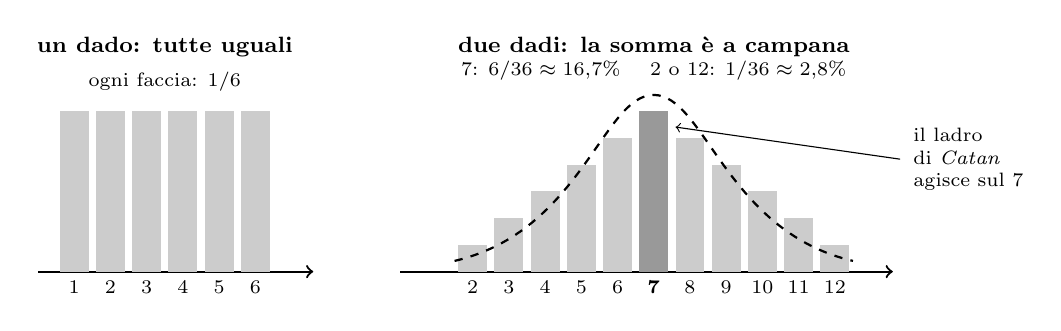
\begin{tikzpicture}[font=\small, x=0.46cm, y=0.34cm]
  % un dado
  \node[font=\footnotesize\bfseries] at (3.5,8.4) {un dado: tutte uguali};
  \draw[thick, ->] (0,0) -- (7.6,0);
  \foreach \v in {1,...,6} {
    \fill[gray!40] (\v-0.4,0) rectangle (\v+0.4,6);
    \node[below, font=\scriptsize] at (\v,0) {\v};
  }
  \node[font=\scriptsize] at (3.5,7.1) {ogni faccia: $1/6$};
  % due dadi
  \begin{scope}[shift={(10,0)}]
    \node[font=\footnotesize\bfseries] at (7,8.4) {due dadi: la somma è a campana};
    \draw[thick, ->] (0,0) -- (13.6,0);
    \foreach \v/\h in {2/1,3/2,4/3,5/4,6/5,8/5,9/4,10/3,11/2,12/1} {
      \fill[gray!40] (\v-0.4,0) rectangle (\v+0.4,\h);
      \node[below, font=\scriptsize] at (\v,0) {\v};
    }
    \fill[gray!80] (6.6,0) rectangle (7.4,6);
    \node[below, font=\scriptsize\bfseries] at (7,0) {7};
    \draw[thick, dashed] (1.5,0.4) .. controls (5,1.5) and (5.6,6.6) .. (7,6.6)
                          .. controls (8.4,6.6) and (9,1.5) .. (12.5,0.4);
    \node[font=\scriptsize, align=center] at (7,7.5) {7: $6/36 \approx 16{,}7\%$ \quad
      2 o 12: $1/36 \approx 2{,}8\%$};
    \node[font=\scriptsize, align=left, anchor=west] at (13.9,4.2) {il ladro\\di
      \emph{Catan}\\agisce sul 7};
    \draw[->, thin] (13.8,4.2) -- (7.6,5.4);
  \end{scope}
\end{tikzpicture}
\caption{Il principio del random controllato: un dado è uniforme, ma la somma di due dadi
non lo è. Il risultato più probabile, il 7, è quello su cui \emph{I Coloni di Catan} mette
il ladro che punisce chi accumula troppe risorse. La linea tratteggiata richiama la curva a
campana che si ottiene sommando molti elementi casuali (la macchina di Galton del video).}
\label{a15:fig:campana}
\end{figure}

\paragraph{Approfondimento: calcolare o simulare.} Schell, in \emph{The Art of Game Design},
usa proprio \emph{Monopoly} come esempio del \emph{metodo Monte Carlo}: quali caselle sono
visitate più spesso? ``Sarebbe quasi impossibile ricavarlo in teoria'', ma una semplice
simulazione che lancia i dadi e muove le pedine qualche milione di volte risponde in pochi
minuti. È il terzo modo di calcolare una probabilità, accanto ai due di Diego: quando il
sistema è troppo intrecciato per l'albero o per la moltiplicazione, si prova, molte volte,
e si contano i risultati. Lo stesso Schell ricorda (è una delle sue ``regole'' della
probabilità) che una cosa è la probabilità reale e un'altra quella \textbf{percepita} dai
giocatori: chi ha provato tre volte un attacco senza mai colpire tende a concludere che
``non colpisce mai''. Per chi progetta, conta anche la seconda.

% ---------------------------------------------------------------------
\section{Le nove combinazioni: input, output, combinato}
\label{a15:sec:nove}

``Ora, il random nei videogiochi e nei giochi da tavolo si usa in tre modi: come
\textbf{input}, come \textbf{output} o \textbf{combinato}.'' È la prima cosa da capire. E
ciascuno dei tre momenti può usare ciascuno dei tre tipi di random visti prima: un input
può essere random vero, pseudo-random o random controllato, e lo stesso vale per l'output.
Ne vengono \textbf{nove combinazioni} possibili (tabella~\ref{a15:tab:nove}).

La differenza tra i tre momenti sta tutta \textbf{nella posizione della casualità rispetto
alla decisione del giocatore} (figura~\ref{a15:fig:momento}): prima della decisione
(l'input: il caso stabilisce \emph{con che cosa} si gioca), dopo la decisione (l'output:
il caso stabilisce \emph{come va} ciò che si è deciso), o entrambe nella stessa decisione
(il combinato).

\begin{figure}[htbp]
\centering
\begin{tikzpicture}[
  font=\small,
  a15box/.style={draw, thick, rounded corners=3pt, minimum height=0.9cm, text width=2.4cm,
                 align=center},
  a15rnd/.style={draw, thick, dashed, rounded corners=3pt, minimum height=0.9cm,
                 text width=2.4cm, align=center, fill=gray!15},
  a15arr/.style={-{Stealth[length=2.6mm]}, thick}
]
  % input
  \node[font=\footnotesize\bfseries, anchor=east] at (-0.3,0) {input};
  \node[a15rnd] (i1) at (1.4,0) {caso\\{\footnotesize carte, setup}};
  \node[a15box] (i2) at (4.8,0) {\textbf{decisione}};
  \node[a15box] (i3) at (8.2,0) {risultato\\{\footnotesize certo}};
  \draw[a15arr] (i1) -- (i2); \draw[a15arr] (i2) -- (i3);
  % output
  \node[font=\footnotesize\bfseries, anchor=east] at (-0.3,-1.6) {output};
  \node[a15box] (o1) at (1.4,-1.6) {situazione\\{\footnotesize nota}};
  \node[a15box] (o2) at (4.8,-1.6) {\textbf{decisione}};
  \node[a15rnd] (o3) at (8.2,-1.6) {caso\\{\footnotesize successo, entità}};
  \draw[a15arr] (o1) -- (o2); \draw[a15arr] (o2) -- (o3);
  % combinato
  \node[font=\footnotesize\bfseries, anchor=east] at (-0.3,-3.2) {combinato};
  \node[a15rnd] (c1) at (1.4,-3.2) {caso\\{\footnotesize la carta pescata}};
  \node[a15box] (c2) at (4.8,-3.2) {\textbf{decisione}};
  \node[a15rnd] (c3) at (8.2,-3.2) {caso\\{\footnotesize il danno da 0 a $n$}};
  \draw[a15arr] (c1) -- (c2); \draw[a15arr] (c2) -- (c3);
  \node[font=\footnotesize, text width=11cm, align=center] at (4.2,-4.5) {grigio
    tratteggiato: dove entra la casualità. Nel combinato i due momenti stanno
    \emph{nella stessa decisione}, non in fasi diverse del gioco};
\end{tikzpicture}
\caption{I tre momenti della casualità rispetto alla decisione del giocatore. L'input
``inietta'' il caso prima che il giocatore scelga; l'output lo mette dopo, sul successo o
sull'entità del risultato; il combinato fa entrambe le cose nella stessa decisione.}
\label{a15:fig:momento}
\end{figure}

\begin{table}[htbp]
\centering
\small
\begin{tabular}{@{}>{\raggedright\arraybackslash}p{2.3cm}>{\raggedright\arraybackslash}p{3.7cm}>{\raggedright\arraybackslash}p{3.7cm}>{\raggedright\arraybackslash}p{3.7cm}@{}}
\toprule
 & \textbf{Random vero} & \textbf{Pseudo-random} & \textbf{Random controllato} \\
\midrule
\textbf{Input} & pescare da un mazzo appena mischiato (poker a cinque carte) & pescare
  sapendo che cosa è già uscito (Texas Hold'em, stoppa, briscola contata) & mazzi costruiti
  per pescare ciò che serve (i mazzi \emph{combo} di \emph{Magic}) \\
\addlinespace
\textbf{Output} & il D20 della palla di fuoco & l'esito tirato da un'app o da un computer &
  il dado con modificatore $+2$ (``sotto il 3 non vai'') \\
\addlinespace
\textbf{Combinato} & pesco una carta e il suo danno è random & la stessa cosa gestita da
  un'app & \emph{push your luck}, scelte tra tre, dadi forgiati \\
\bottomrule
\end{tabular}
\caption{Le nove combinazioni tra i tre tipi di random e i tre momenti della decisione,
con un esempio per casella tratto dalla lezione (alcune caselle sono ricostruite dagli
esempi successivi: Diego elenca le combinazioni, ma non le illustra una per una).}
\label{a15:tab:nove}
\end{table}

% ---------------------------------------------------------------------
\section{L'input random}
\label{a15:sec:input}

\subsection{Che cos'è: il caso prima della decisione}

La definizione sulla slide: l'input random è ``\emph{the injection of chance before the
player makes a decision}''; fornisce condizioni incerte, o risorse, con cui il giocatore
deve poi lavorare strategicamente. È \textbf{l'aggiunta di un elemento casuale, o
statisticamente basato, che crea incertezza nelle condizioni o nello stato del gioco}, e con
cui i giocatori devono poi gestire il resto della partita.

``Sembra complesso, ma il modo più facile è \textbf{pescare le carte}.'' Molti giochi dicono
``all'inizio del turno pesca una carta'': quella carta è randomica, o pseudo-randomica.

\paragraph{Poker a cinque carte e Texas Hold'em.} Nel poker ``all'italiana'', quello a
cinque carte\footnote{Diego cerca il nome (``non briscola\ldots{} poker''): ``di tanto mi
vengono i giochi italiani''.}, non si ha idea di che cosa si peschi: si pescano le carte, si
guardano, si decide. È input \textbf{random}. Nel \textbf{Texas Hold'em} la mano è invece
\textbf{pseudo-random}: dalle carte scoperte sul tavolo si ricavano informazioni sul resto
del mazzo.

\paragraph{Contare le carte.} Diego chiede che cosa voglia dire \textbf{contare le carte} a
poker, e Jacopo, ``rivela i segreti'', risponde: pur non essendo un giocatore di poker, si
conta la quantità di carte rimaste e si calcola la probabilità che esca quella che serve,
per esempio il quarto asso. ``Esatto'': se i quattro assi sono già sul tavolo, la
probabilità che un altro giocatore abbia un asso è zero. È semplice, ma è importante,
perché trasforma il caso in informazione.

\subsection{La stoppa: un input che diminuisce nel tempo}

C'è ``un gioco italiano che io cito sempre'', perché è interessantissimo proprio su questo:
la \textbf{stoppa}. È un gioco di carte del Sud Italia, di cui non si sa bene chi l'abbia
inventato: un ``poker italiano'' con una caratteristica particolare. Si gioca \textbf{a
fasi}. Nella prima fase ogni giocatore riceve \textbf{tre carte}, che hanno punteggi come nel
poker: si può avere una mano buona o cattiva.

\paragraph{Una mano.} Diego, Jacopo e Davide giocano. Diego ha una buona mano e rilancia;
Davide ha una buona mano e vede; Jacopo ha una brutta mano e ``si fa i fatti suoi''. Diego e
Davide continuano a rilanciare, senza pescare altre carte, finché nessuno rilancia più e si
rivelano le carte. Diego ha un \textbf{tris di 7}, un buon punteggio\footnote{Nella
trascrizione ``il 7 vale 21 punti nella stoppa, quindi 7, 21, 42, 63'': i valori sono
riportati come detti, ma la sequenza è confusa e non permette di ricostruire con certezza il
sistema di punteggio.}; Davide rivela di aver bluffato, e Diego vince.

\paragraph{Le carte restano.} Nel poker a questo punto si rimischia, fine. Nella stoppa,
invece, \textbf{tutti i giocatori tengono le proprie carte}, Jacopo compreso, e le mettono
da parte. Diego ha vinto la mano, ma ora tutti sanno che quei tre 7 non sono più nel mazzo e
che li ha lui; e Diego sa che cosa aveva Davide, ma non che cosa aveva Jacopo. Si continua
così finché il mazzo finisce e ciascuno ha \textbf{dieci carte}: a quel punto si devono
scegliere tre carte tra le proprie dieci per fare la mano migliore.

\paragraph{Vincere vuol dire rivelarsi.} Che cosa significa? Che \textbf{più si è vinto nelle
mani precedenti, più si è rivelata la propria mano finale}: se si è vinto tanto, tutti hanno
visto le carte, e sanno esattamente che cosa c'è fra quelle dieci. Chi ha perso, o ha
nascosto sempre le carte (come Jacopo), resta un mistero. È \textbf{un esempio di input
random che diminuisce nel tempo}: si parte da un input del tutto casuale, l'intero mazzo, e
pian piano l'informazione cresce e il caso si riduce.

\subsection{\emph{Magic}: trasformare il random in pseudo-random}

Diego chiede chi gioca a \textbf{\emph{Magic: The Gathering}}, \emph{Yu-Gi-Oh!} o altri
collezionabili; Jacopo gioca a \emph{Magic}. Una delle caratteristiche di \emph{Magic} è
proprio \textbf{partire dal mazzo randomico e trasformarlo in pseudo-randomico}, con carte che
permettono di \textbf{controllare la pescata}. Jacopo fa un esempio: ci sono carte che
fanno guardare le prime tre del mazzo, o rimischiare il mazzo; ``hai tanto controllo''.
``Esattamente.'' I cosiddetti \textbf{mazzi \emph{combo}}, che vincono se ottengono una certa
combinazione di carte, non sperano di pescare per caso la carta giusta: inseriscono tutta
un'altra serie di carte che trasformano il mazzo in pseudo-randomico e \textbf{aumentano
statisticamente la probabilità} di ottenere ciò che serve.

\paragraph{Investire risorse per controllare il caso.} L'input random, quindi, è qualcosa
che avviene \textbf{prima} delle decisioni e che i giocatori usano \textbf{per} decidere; e
molti giochi lo collegano alla possibilità di \textbf{controllare quella randomicità a
proprio vantaggio}, di solito \textbf{investendo risorse}. Un gioco inventato: ogni turno si
pesca una carta e si fa ciò che dice. Diego pesca ``3 risorse'' e passa; Oksana pesca ``5
risorse''; Diego (lo studente) pesca ``5 risorse''. Poi Diego può scegliere: pescare, o
investire le risorse in un'abilità speciale che dal turno successivo gli fa \textbf{vedere
due carte e sceglierne una}. È una forma tipica di \textbf{progressione} nei giochi da
tavolo: si inizia con un input completamente casuale (random vero) e lo si trasforma in
\textbf{random controllato}, diventando più forti. Guadagnando abilità, sbloccando risorse,
si ottiene \textbf{più controllo}.

\subsection{\emph{Monopoly}: dal random al random controllato}

``Chi riesce a dirmi dove sta la trasformazione da random a controllato in
\emph{Monopoly}?'' Silenzio (``non abbiamo la bellissima botta di Monopoly'', scherza
qualcuno). Diego aiuta: come si guadagnano soldi a \emph{Monopoly}? Gli studenti rispondono:
quando qualcuno finisce sulle tue proprietà; quando passi dal via (200); quando peschi la
carta giusta negli imprevisti. Il via non si controlla, e lo si esclude; gli imprevisti
nemmeno. Resta un elemento, e uno studente lo trova: \textbf{gli scambi}, dove ``c'è del
controllo'', perché si decide, si contratta sul valore effettivo, sui soldi, sulle ipoteche.
``Bravo! Si gioca su quello.''

\paragraph{Il gioco in una frase.} Non si può sapere dove finirà un avversario, ma \textbf{se
si possiede il 70\% delle proprietà, ci finirà}. ``E questo è il gioco del
\emph{Monopoly}'': trasformare il random vero in random controllato, \textbf{solo in versione
input}. Per questo, secondo Diego, \emph{Monopoly} è un gioco ``battuto'': esiste una
strategia ottimale, la si può cercare (``\emph{Monopoly how to play perfectly}'') e diventare
campioni\footnote{È un'espressione forte: \emph{Monopoly} non è un gioco ``risolto'' nel
senso matematico in cui lo sono, per esempio, la dama o il tris, anche perché contiene una
forte componente di trattativa. Esistono però analisi molto approfondite (con le catene di
Markov) su quali proprietà rendono di più e quando conviene costruire, ed è a queste che
Diego si riferisce.}. Uno dei principi è comprare le caselle che stanno ``intorno al 7''
rispetto ai punti di passaggio più frequenti, perché statisticamente ci si finisce sopra.
``Può sembrare banale, riduttivo'', ma è uno dei giochi di maggior successo della storia, e
si basa soltanto sul dare ai giocatori la possibilità, con la loro competenza, di
trasformare l'input random in random controllato.

\subsection{Ruoli nascosti e \emph{setup} variabili}

Chi conosce \textbf{\emph{Secret Hitler}}, \textbf{\emph{The Resistance}} o \textbf{\emph{Lupus
in fabula}} (\emph{Werewolf})? Jacopo conosce \emph{Secret Hitler}; Davide conosce meglio
\emph{Werewolf}: c'è un gruppo che deve eliminare gli altri, e quelli che si conoscono tra
loro sono in svantaggio numerico. ``Esattamente.'' Qui il punto di partenza è che
\textbf{il ruolo è casuale}: si può essere nazista o della resistenza in \emph{Secret
Hitler}, lupo mannaro o umano in \emph{Werewolf}; ma poi si deve giocare, e l'abilità di
giocare dipende dal ruolo avuto. Lo stesso vale per il videogioco \textbf{\emph{Among
Us}}\footnote{Nella trascrizione ``da Mongas''.}, con gli infiltrati e gli altri: il gioco si
basa tutto sull'individuare chi è l'altro \textbf{partendo dall'input random}.

\paragraph{Gli scenari.} Infine, i \textbf{\emph{variable setup}}: chi gioca a D\&D o ad altri
giochi di ruolo da tavolo sa che gli scenari sono letteralmente un input random: si parte da
uno scenario che dà delle possibilità. L'input random è quindi \textbf{la capacità del
designer di creare una situazione più o meno controllata}, usando le tecniche viste (il
random controllato in particolare), per dare \textbf{scelte interessanti} ai giocatori.

\subsection{La briscola: il rischio di contare troppo}

Un altro esempio, la \textbf{briscola}, che ``penso conosciate tutti''. La primissima cosa che
avviene è \textbf{rivelare la briscola}: e la propria mano può passare ``da una schifezza a
meravigliosa'' in base al seme, ma anche in base alla carta stessa che è stata rivelata. Sapere
che l'ultima carta è l'asso di briscola, o il tre, o il due (gli estremi, le carte che valgono
tanto e quelle che ``non valgono una ceppa'') cambia completamente la partita.

\paragraph{Il ``mago'' delle superiori.} Chi ha giocato alle superiori, quando la briscola
``era lo standard'', ricorderà che c'è sempre qualcuno che all'ultimo giro dice: ``tu avrai
un carico; tu hai sicuramente due carte di briscola, probabilmente il 7''. È un mago? ``Un Da
Vinci incompreso? No.'' \textbf{Ha contato le carte}, in base a come si è giocato. Sta
\textbf{comprendendo l'input random e togliendolo}, controllandolo. Se si sanno tutte le carte
che tutti hanno in mano, si può giocare la partita perfetta; e infatti a quel punto quella
persona dice: ``tagliamo corto: tu vincerai la seconda mano, io la prima, voi la terza''. Ed è
così, perché giocare diversamente sarebbe giocare male.

\paragraph{Il rischio.} Ecco il rischio dell'input random: \textbf{se si dà al giocatore
troppo controllo sull'input, il random sparisce}, perché il gioco diventa prevedibile. E una
cosa prevedibile è come il finale della briscola: ``è inutile che giochiamo le ultime tre
mani''.

\subsection{I vantaggi dell'input random}

Diego passa ai pro e ai contro, con le definizioni in inglese sulle slide (``i cosi ve li
lascio lì'').

\paragraph{\emph{Meaningful decision making}.} ``\emph{Players interpret random setup and make
optimal choices with constraints}''; sulla slide c'è anche l'esempio di \textbf{\emph{7
Wonders}}, con il \emph{draft} delle carte e le scelte tra opzioni casuali. Se il punto di
partenza è casuale, i giocatori devono fare \textbf{scelte complesse}, perché non possono
avere la partenza ottimale né sapere come andranno le cose. Questo aggiunge valore
\textbf{tattico}, non strategico, e Diego insiste sulla differenza:
\begin{itemize}
  \item \textbf{strategico} vuol dire \textbf{nel lungo periodo}: una strategia di guerra è
        ``l'anno 1 invaderemo e raccoglieremo risorse, l'anno 2 faremo questo'';
  \item \textbf{tattico} è \textbf{la battaglia}: ``ci stiamo sparando addosso'', si decide
        minuto per minuto.
\end{itemize}
Le scelte di input random sono \textbf{tattiche}: si pescano le carte e si ha qualche minuto
per decidere, non tre ore. Nei giochi di carte, \textbf{il mazzo è una scelta strategica}
(lo si è costruito con il \emph{deck building}); \textbf{la mano che capita è tattica}: può
essere perfetta o, ``sfiga vuole'', terrificante.

\paragraph{\emph{Replayability}: \emph{Cosmic Encounter}.} Una partenza casuale
\textbf{aumenta la rigiocabilità}, perché ogni tanto capita la mano fortunata, o quella
strana. L'esempio è \textbf{\emph{Cosmic Encounter}}, che nessuno conosce (``la maggior parte
della gente dice di no''): ``se siete interessati al random, è il gioco che dovreste studiare
più di tutti''. Le regole di base sono semplicissime: ogni giocatore ha \textbf{5 pianeti}, e
su ogni pianeta ci sono navi spaziali. Diego (rosso) attacca Jacopo (verde) per conquistargli
un pianeta, con 10 navi; Jacopo ne ha 5 sul pianeta. Jacopo gioca una carta $+10$, e arriva a
15; Diego gioca una carta $+5$, e arriva a 25 (il conto a voce è un po' confuso, ma il senso è
chiaro): vince Diego, che conquista il pianeta. ``Che gioco schifoso'', direte; ``che palle!''
Questa è solo la base.

\paragraph{Gli alieni.} La cosa grande di \emph{Cosmic Encounter} è che \textbf{ognuno ha un
alieno}, e ogni alieno ha \textbf{un'abilità che cambia completamente la partita}. Con tutte
le espansioni, dice Diego, ce ne sono ``qualcosa come 900''; ogni partita è una combinazione
di cinque alieni, e le possibilità sono enormi\footnote{Diego dice ``900 alieni'' e poi ``5
elevato alla 900''. Il numero di alieni, anche con tutte le espansioni, è dell'ordine di
qualche centinaio; e il conto corretto per scegliere 5 alieni fra $n$ è il coefficiente
binomiale $\binom{n}{5}$, non $5^{n}$. Anche così il numero resta enorme: con 200 alieni le
combinazioni di cinque sono circa 2,5 miliardi.}. Due esempi da partite vere.
\begin{itemize}
  \item Una partita tra Diego, il suo migliore amico e la moglie di lui. Diego ha un alieno che,
        scartando una carta, ne recupera una dal proprio cimitero; la moglie dell'amico può
        \textbf{nominare una carta} nella mano avversaria e, se c'è, rubarla; l'amico può far
        scartare a tutti la mano e far ripescare sette carte a caso. I poteri si
        contrastavano a vicenda: se Diego usava la sua abilità, gli altri vedevano quale carta
        recuperava; la moglie dell'amico allora la nominava (``secondo me hai questa carta in
        mano?''); e se l'amico vedeva che la moglie aveva preso una carta forte, faceva
        scartare tutto. ``Questa combinazione non era mai successa.''
  \item Un alieno che la trascrizione chiama \textbf{``Ace''}, ``il campione''\footnote{Il nome
        dell'alieno non è verificabile; il capitolo lo riporta come detto.}, per vincere deve
        conquistare \textbf{un solo pianeta} invece di cinque. Facilissimo? No: diventa
        \textbf{il nemico pubblico numero uno}, perché tutti sanno che se conquista anche solo
        un pianeta vince la partita. Il gioco si trasforma da tutti contro tutti in
        \textbf{quattro contro uno}, e chi ha quell'alieno deve giocare in modo super difensivo
        e aspettare il momento giusto.
\end{itemize}
In base agli alieni pescati, la partita cambia completamente: l'input random crea
``infinita'' rigiocabilità.

\paragraph{\emph{Encouraging skill}: livellare le abilità.} ``Questo è estremamente
importante'': un input random \textbf{può livellare la differenza di abilità} tra i
giocatori. Se un giocatore mediocre gioca contro un campione, e il campione ha avuto una mano
sfortunata o il mediocre una mano fortunata, la differenza si assottiglia.

\paragraph{L'esercizio del torneo di poker.} Diego propone un esperimento mentale. Non avete
mai giocato a poker, in nessuna versione; siete finiti, in qualche modo, nella finale del
torneo più importante del mondo, contro i tre campioni del mondo, e in palio ci sono 10
milioni di euro. \textbf{Quale strategia applicare per ridurre la differenza di abilità}?
``Pensateci.'' Uno studente propone di contare le carte; ma i campioni sanno contare meglio.
Allora: che cosa rende bravo un giocatore professionista? Contare le carte, e soprattutto
\textbf{prevedere che cosa faranno gli altri}, leggerne il comportamento; la \emph{poker
face}, la capacità di non mostrare emozioni. Imitare il loro comportamento? Sanno farlo
meglio. Davide ride: ha capito. La risposta è \textbf{non guardare le proprie carte}. ``Non
puoi intuire come io gioco, se nemmeno io so come sto giocando.'' Tutta l'abilità degli
avversari nel prevedere le mosse si annulla, e la partita si riduce alla \textbf{fortuna}: se
le carte sono buone si vince, altrimenti si perde.

\paragraph{La fortuna del principiante.} È quella che si chiama, appunto, \textbf{fortuna del
principiante}: spesso qualcuno ha perso perché cercava di applicare tecniche avanzate contro
qualcuno che non sapeva che cosa stesse facendo, ed è rimasto fregato. Se lo si fa davvero
in un torneo, le probabilità aumentano, ``ma tutti vi odieranno tantissimo'': è una strategia
conosciuta e i professionisti la detestano, perché vogliono giocare con la \emph{poker face}.
``Però non è tecnicamente illegale.''

\subsection{I rischi dell'input random}

``Non è tutto oro quel che luccica'': ci sono dei pericoli.

\paragraph{La \emph{turn one win}.} Se le possibilità di partenza sono troppo varie, è
possibile vincere \textbf{al primo turno} per pura fortuna. Un esempio ``che fa veramente
ridere'': la madre di Diego partecipa a un torneo di \textbf{scala 40}, arriva in finale,
l'avversaria mischia, lei taglia, pesca le carte e ha la \textbf{chiusura in mano}: tredici
carte perfette, vince il torneo. ``Non ci puoi fare niente.'' Nella scala 40 non è un
problema, perché succede raramente; ma la domanda da porsi, con l'input random, è
\textbf{quanto è possibile essere del tutto sfortunati o del tutto fortunati}.

\paragraph{Il solitario di Diego.} Da studente, Diego aveva provato a fare un
\textbf{solitario}: si disponevano delle carte sul tavolo e si cercava di fare una serie di
cose. Il problema: \textbf{se la carta negativa non finiva in uno dei quattro angoli, il
solitario era impossibile da risolvere}. Era una condizione di partenza troppo sbilanciata
(una \emph{uneven condition} troppo aggressiva): non è giusto perdere per questo. La
soluzione fu togliere la carta ``sfigata'' dal mazzo da mischiare e farla \textbf{aggiungere
dal giocatore in uno dei quattro angoli, a sua scelta}, rimuovendo un'altra carta. Così la
condizione si verificava sempre, e il solitario funzionava.

\paragraph{La morale.} Si possono inserire elementi che \textbf{controllano l'input random e
lo depotenziano} quando è ``troppo rotto'': lo riducono di potenza, lo rendono meno efficace,
oppure lo giustificano. In \emph{Arkham}, se nella mano iniziale c'è una
\textbf{debolezza}, la si toglie, la si rimischia nel mazzo e si pesca un'altra carta:
perché iniziare la partita con una debolezza in mano ``è finita''. La mischiata è casuale,
``ma se è proprio sfiga, non va bene''. Anche \emph{Magic} ha qualcosa del genere, il
\textbf{\emph{mulligan}}, su cui la lezione tornerà.

\paragraph{La paralisi da analisi.} Succede soprattutto con giochi nuovi o giocatori nuovi:
se l'input random è troppo forte (cinque carte in mano, più cinque pedine casuali, più cinque
altre cose casuali: venti elementi casuali), è \textbf{troppa roba da calcolare per la
tattica}. ``Ricordatevi: strategia contro tattica.'' Se si hanno cinque minuti per decidere e
venti cose casuali da valutare, non ce la si fa. In questi casi alcuni elementi devono
essere \textbf{non casuali}: per esempio il numero di risorse; o il mazzo costruito dal
giocatore, così che la pescata è casuale ma il contenuto del mazzo è noto; o
\textbf{l'obiettivo}. Ci sono giochi in cui anche l'obiettivo è casuale, e non si sa che cosa
fare finché non lo si è pescato.

\paragraph{La riduzione della strategia, o una falsa strategia.} Se \textbf{tutto} è casuale,
il gioco è rigiocabile ma non profondo: è ``una serie di condizioni casuali''. Come lo si
limita? Con \textbf{obiettivi non casuali}. Se la partenza è casuale ma l'obiettivo no, si
può sempre costruire una strategia verso l'obiettivo; se sono casuali entrambi, forse no.

\paragraph{Il controllo limitato.} Infine il \textbf{\emph{limited player control}}: se tutto
è casuale, il giocatore non ha scelta. L'input random dovrebbe stare \textbf{all'inizio}, e
poi la decisione deve essere del giocatore.

Nessun dubbio. Diego propone la pausa, ma gli studenti preferiscono continuare: ``facciamo
l'output e poi dopo facciamo la pausa''.

\subsection{Le linee guida}

Prima di passare all'output, Diego riassume l'input random con qualche indicazione pratica
(tabella~\ref{a15:tab:input}).

\paragraph{Dove guardare.} Il \emph{deck building}, i giochi
``\emph{layer}''\footnote{Così nella trascrizione: potrebbe essere ``\emph{legacy}'',
``\emph{player}'' o altro; non è ricostruibile.}, i \textbf{giochi asimmetrici} e il
\textbf{\emph{drafting}} sono tutti esempi di ottimi input random da prendere come
riferimento; la slide ne elenca sette, ``come sette caratteristiche''.

\paragraph{La regola unica.} Se si vuole ridurre tutto a una sola regola: \textbf{l'input
random deve far sentire il giocatore più potente}, offrendogli \textbf{più scelte} di quelle
che avrebbe senza, \textbf{ma non deve togliergli l'\emph{agency}}. Il giocatore non deve
sentire di non avere controllo su ciò che avviene: non che il risultato sia necessariamente
``corretto'', ma che \textbf{si senta} in controllo. Ed è qui che entra il random controllato:
\textbf{i giochi basati sull'input random nascono input e finiscono controllati}.

\paragraph{Le cento partite.} Un suggerimento personale: quando si fa un gioco con input
random, \textbf{si giochino cento partite}. Se nel \textbf{30\% delle vittorie o più} conta la
fortuna, il gioco è troppo basato sulla fortuna; \textbf{la fortuna dovrebbe influire sul
20\% delle vittorie}\footnote{Diego non dice come stabilire, in pratica, se una vittoria
``è dovuta alla fortuna''. Un modo possibile è far giocare insieme persone di abilità nota e
contare quante volte vince chi è meno esperto, o confrontare i risultati con quelli di una
strategia casuale; ma è un'aggiunta del capitolo.}.

\paragraph{L'interessante prima del giusto.} E un altro consiglio ``da persona che fa questa
roba da tanti anni'': \textbf{con il random, favorite l'interessante invece del giusto}. Dire
``questo random è bilanciato'' è meno funzionale, in \emph{game design}, che dire ``questo
random è interessante''. Se poi si scopre che è troppo sbilanciato, \textbf{si aggiunge una
regola per bilanciarlo}, come la debolezza di \emph{Arkham} o il \emph{mulligan}. Pescare
carte a caso è interessante; e ``interessante vince sempre rispetto a giusto''.

\begin{table}[htbp]
\centering
\small
\begin{tabular}{@{}>{\raggedright\arraybackslash}p{3.4cm}>{\raggedright\arraybackslash}p{5.0cm}>{\raggedright\arraybackslash}p{5.2cm}@{}}
\toprule
\textbf{Aspetto} & \textbf{Che cosa succede} & \textbf{Esempi e rimedi} \\
\midrule
\multicolumn{3}{@{}l}{\emph{Vantaggi}} \\
Decisioni sensate & la partenza imperfetta chiede scelte \textbf{tattiche} & la mano
  (tattica) contro il mazzo (strategico); \emph{7 Wonders} \\
\addlinespace
Rigiocabilità & ogni partenza è diversa & gli alieni di \emph{Cosmic Encounter} \\
\addlinespace
Livellare le abilità & la mano fortunata avvicina principiante e campione & il poker
  giocato senza guardare le carte \\
\midrule
\multicolumn{3}{@{}l}{\emph{Rischi}} \\
\emph{Turn one win} & si vince (o si perde) per la sola partenza & la chiusura in mano a
  scala 40; il solitario di Diego: la carta ``sfigata'' piazzata dal giocatore; le
  debolezze di \emph{Arkham}; il \emph{mulligan} \\
\addlinespace
Paralisi da analisi & troppi elementi casuali da valutare & rendere fissi risorse,
  contenuto del mazzo, obiettivo \\
\addlinespace
Falsa strategia & tutto casuale: rigiocabile ma non profondo & obiettivi non casuali \\
\addlinespace
Poco controllo & il giocatore non sceglie & il caso all'inizio, poi la decisione \\
\addlinespace
Troppo controllo & il random sparisce, tutto è prevedibile & il finale della briscola \\
\bottomrule
\end{tabular}
\caption{L'input random in sintesi. Regola d'oro: nasce input e finisce controllato, e deve
far sentire il giocatore più potente senza togliergli l'\emph{agency}; la fortuna dovrebbe
decidere circa il 20\% delle vittorie, non il 30\% o più.}
\label{a15:tab:input}
\end{table}

\paragraph{Approfondimento: caso e abilità secondo il pubblico.} Brathwaite e Schreiber, in
\emph{Challenges for Game Designers}, dedicano un capitolo all'equilibrio tra caso e
abilità che parte esattamente dalle due idee di Diego. La prima: \textbf{il pubblico}. I
bambini piccoli non hanno ancora gli strumenti per decisioni strategiche e giocano volentieri
a giochi di pura fortuna (``spesso sono convinti che tirare numeri alti con i dadi sia
un'abilità''); i giocatori competitivi vogliono che nessun tiro di dado rovini una giocata
perfetta; i giocatori ``sociali'' tollerano molta più fortuna; le famiglie hanno bisogno di
un po' di fortuna perché i bambini possano battere gli adulti. La seconda: \textbf{la fortuna
livella}. ``Più fortuna c'è in un gioco, più il campo è livellato'': se vince sempre il più
bravo, le uniche partite interessanti sono quelle tra pari; e un po' di caso toglie anche un
po' di amarezza alla sconfitta, perché chi vince può sentirsi più abile e chi perde può
dare la colpa ai dadi. Il libro propone anche i segnali da cercare nei \emph{playtest}: se
i giocatori si annoiano, forse c'è troppa fortuna (si converta qualche elemento casuale in
una decisione); se un giocatore stravince sugli altri, forse c'è troppa abilità (si aggiunga
un po' di casualità, o un meccanismo di recupero). E, come Diego, suggerisce di
\textbf{scambiare} caso e decisione: ``pagate 50 prima di tirare, e tirate tre dadi
scegliendone due'' è il loro esempio su \emph{Monopoly}, ed è esattamente un input random
reso controllato in cambio di risorse.

% ---------------------------------------------------------------------
\section{L'output random}
\label{a15:sec:output}

\subsection{Che cos'è: il caso dopo la decisione}

Diego apre con alcune GIF che gli piacciono (giocatori di \emph{Commander} e una giocatrice
che gioca ``un sacco di mazzi \emph{combo}''). L'output random è \textbf{esattamente
l'opposto} dell'input: il random non è sulle risorse che si hanno, ma \textbf{sul risultato
dell'azione}.

\paragraph{La palla di fuoco.} Il modo più semplice per definirlo è \textbf{D\&D}. Ho
un'abilità: lanciare una \textbf{palla di fuoco} in faccia all'avversario. Se colpisco o meno
quel giocatore, o quel PNG, dipende dai dadi: con 15 o più colpisco, con 14 o meno no; e il
danno dipende dal numero di dadi che lancio\footnote{È una semplificazione: nelle regole
della quinta edizione di D\&D, contro la palla di fuoco è il bersaglio a tirare un
\emph{tiro salvezza} su Destrezza, che dimezza il danno, e il danno è $8d6$. Il principio
che Diego illustra non cambia: la decisione è certa, l'esito è affidato ai dadi.}. Qui non è
la decisione, né l'abilità, a essere random: so di avere la palla di fuoco, ho deciso di
usarla, e ne ho il totale controllo, perché fa parte del mio personaggio (``non è che ho
pescato la carta palla di fuoco''). Ma \textbf{se colpisco e quanto danno faccio}, quello è
random.

\paragraph{La definizione.} L'output random è quando \textbf{la casualità avviene dopo che il
giocatore ha preso una decisione}. Di solito influenza \textbf{il successo o il fallimento},
oppure \textbf{la magnitudo}, cioè l'entità di quel successo o fallimento. Il giocatore prima
si \textbf{impegna} (\emph{commits}) in una decisione, un piano, una tattica; poi il caso gli
dice se ha funzionato e, nel caso, quanto. È all'estremo opposto dello spettro: l'input dice
quali azioni si potrebbero compiere in quel momento; l'output dice ``no, le azioni le hai già
tutte, ma il loro risultato non è scontato''.

\paragraph{La domanda di Jacopo: \emph{Betrayal}.} Jacopo chiede di un gioco come
\textbf{\emph{Betrayal at House on the Hill}}\footnote{Nella trascrizione ``B-Train'' e
``Betrayal''. Più avanti Diego lo chiama ``Betrayal of the House of the Hill''.}, un gioco di
piazzamento di tessere: si sceglie di muoversi e si pesca la tessera, e su alcune tessere ci
sono i simboli degli eventi, o si pesca un oggetto. È input e output insieme, o solo input?
Diego risponde che è \textbf{combinato}, e spiega il criterio. Quando peschi la tessera, è
input: il caso viene prima e non hai nemmeno deciso che cosa uscirà. Poi, visto il risultato,
prendi una decisione: e \textbf{se quella decisione può avere esiti diversi, c'è anche
l'output}. Se la tessera dice ``prenditi tre pizze'', è solo input; se dice ``lancia un dado
per sapere quante pizze'', è combinato. ``Hai fatto benissimo'': la lezione è un dialogo,
``intervenite quando volete''.

\paragraph{Altri esempi.} Il lancio dei dadi per un'azione in D\&D; il \textbf{Risiko} (Diego
dice \emph{Risk}, ``che sarebbe Risiko all'italiana''); i \textbf{segnalini del sacchetto} di
\emph{Arkham}: ``voglio menarlo''; peschi il segnalino $-3$, la tua abilità scende a 2, troppo
debole, non ci sei riuscito; oppure peschi ``danno critico'', o ``fallimento
critico''\footnote{Diego mescola qui il sacchetto del caos di \emph{Arkham} e il D20 di D\&D:
il racconto dei tre fallimenti critici, uno su venti, riguarda con ogni probabilità il D20.}.
Diego ci ha giocato ``letteralmente ieri'', e un suo amico ha tirato \textbf{tre volte di
seguito un fallimento critico}: ``ma che cacchio, sei proprio sfigato''. È output, perché la
decisione era presa, l'azione fatta, ma non è andata per niente bene. E poi il \textbf{lancio
della moneta}: ``se esce testa mangio l'hamburger, se esce croce prendo una pizza''. La
decisione è presa; il risultato dipende dall'elemento casuale.

\subsection{Perché usarlo: il dramma}

L'input random serve a creare scelte tattiche e a mitigare le differenze di abilità.
\textbf{L'output random serve ad aggiungere il dramma}, ``nel senso proprio del termine,
teatrale''. Quando non so se la mia azione avrà successo, sono teso: \textbf{non sapere crea
tensione per natura}.

\paragraph{\emph{Affari tuoi}.} L'esempio perfetto è ``il gioco dei pacchi su Rai 1''. Per
semplicità ci sono venti pacchi: dieci ``sfigati'' (un peluche da 10 euro, un sacchetto di
noccioline) e dieci ``fighi'' (da 5.000 a 300.000 euro). I concorrenti aprono i pacchi che
scelgono finché ne restano pochi (per esempio cinque, tre positivi e due negativi, o
viceversa); poi arriva un'\textbf{offerta}: ``ti do 40.000 euro e il gioco finisce adesso;
oppure rischi, e magari c'è ancora il pacco da 300.000''. Se si sapesse di avere il pacco
sfigato, si accetterebbe al volo; se si sapesse di avere quello da 300.000, si rifiuterebbe.
\textbf{Il dramma sta nel fatto che l'output è sconosciuto}: ``oddio, 40.000 sono tanti
soldi; ma se poi avessero quello da 300.000? E se beccano il calzino?''

\paragraph{\emph{Golden Balls}.} Un altro esempio, ``un capolavoro'', da YouTube:
\textbf{\emph{Golden Balls}}\footnote{Nella trascrizione ``la Golden Ball''. È il quiz
britannico \emph{Golden Balls} (ITV); l'episodio mostrato, con i concorrenti Nick e Ibrahim, è
uno dei più famosi del ``\emph{split or steal}''.}. Due concorrenti hanno collaborato per
accumulare una cifra (in quella puntata circa 13.000 sterline) e ora hanno davanti due
palline: \textbf{dividi} (\emph{split}) e \textbf{ruba} (\emph{steal}). Se entrambi scelgono
dividi, si dividono la somma; se entrambi scelgono ruba, nessuno vince niente; se uno sceglie
ruba e l'altro dividi, chi ha scelto ruba prende tutto. Diego fa sentire lo spezzone: Nick
dice a Ibrahim che sceglierà \emph{steal} al 100\%, e gli chiede di scegliere \emph{split},
promettendo di dividere i soldi con lui dopo lo spettacolo. Ibrahim incredulo: ``dopo che hai
preso \emph{steal}?'' ``Sì.'' Che fare? Fidarsi di una promessa ``nell'aria'', o scegliere
ruba per ripicca, ``e nessuno vince niente''? ``Fidati che i soldi te li do.'' Questa
\textbf{incertezza del risultato crea il dramma}. ``Andatevelo a vedere, se volete sapere come
va a finire.''

\paragraph{I tre vantaggi.} Ne vengono tre punti di forza.
\begin{enumerate}
  \item \textbf{Il dramma e l'intensità emotiva.} Una scelta non sicura spinge l'emotività,
        e ``fare giochi è essere emotivi'': vogliamo che i giocatori provino emozioni, e
        rendere incerto il risultato le spinge al massimo.
  \item \textbf{\emph{High risk, high reward}.} Non avere la certezza del risultato permette
        di dare al giocatore scelte \textbf{molto pericolose ma potenzialmente molto
        vantaggiose}. Se va male, ``chi è causa del suo mal pianga se stesso'': la scelta
        rischiosa l'hai fatta tu. ``Mi è capitato migliaia di volte: se azzecco questa cosa
        vinco; poi la sbaglio e ho perso.'' Con la certezza assoluta di riuscire, sarebbe
        stato noioso.
  \item \textbf{Ridurre la differenza di abilità}, come per l'input: se non sono sicuro di
        batterti, perché potrei avere un colpo di sfortuna, tu resti in partita.
\end{enumerate}

\subsection{Il rischio: troppa sfortuna}

Il rischio è che \textbf{troppa sfortuna dà fastidio}. È ciò che è successo all'amico di
Diego: tre fallimenti critici di fila tolgono al giocatore la sensazione di \emph{agency}
(``una volta va bene, ma tutte e tre le volte non è giusto''). Diego prova a fare il conto con
la calcolatrice: una possibilità su 20, tre volte, ``quindi una su 60'', l'1,6\%; uno
studente lo corregge, le probabilità vanno \textbf{moltiplicate}, ``ah, giusto, è molto più
basso''\footnote{Il conto corretto: $\left(\tfrac1{20}\right)^3 = \tfrac1{8000} =
0{,}0125\%$, cioè circa una volta su ottomila serie di tre tiri. È lo stesso errore che il
modo ``visivo'' della sezione~\ref{a15:sec:calcolo} aiuta a evitare: tre eventi indipendenti
si moltiplicano, non si sommano.}. ``Quindi è una cosa folle.'' Troppo risultato casuale
toglie ai giocatori la sensazione di avere effetto sul gioco: fanno la loro strategia, la loro
tattica, e poi non funziona mai perché hanno sfortuna. Per questo esistono \textbf{tecniche
di mitigazione}, che Diego mostra subito dopo.

\subsection{Quando: poco all'inizio, di più verso la fine}

Mentre l'input è presente all'inizio e poi diventa controllato, \textbf{l'output random non
dovrebbe essere presente all'inizio}. Qui la trascrizione si interrompe\footnote{Una stringa
ripetuta (``Output transcript'') copre una parte della spiegazione. Il senso è ricostruibile
da ciò che Diego dice dopo la pausa, quando disegna le due curve: ``l'output è l'opposto: ne
ho poco all'inizio e diventa medio a fine partita, per dare quel momento di dramma''
(figura~\ref{a15:fig:curve}). È andato perso anche l'inizio dell'esempio che segue.} e
riprende nel mezzo di un esempio, che mostra come inserire l'output alla fine \textbf{senza
annullare} ciò che è avvenuto prima.

\paragraph{Il sacchetto finale.} Siamo nella fase finale, e il gioco dice: per ogni 10 risorse
accumulate, metti nel sacchetto un segnalino del tuo colore (verde Diego, rosso Davide). Diego
ha 100 risorse, Davide 200: Davide mette 20 segnalini, Diego 10. Poi si estrae un segnalino, e
chi viene estratto vince. Diego ha comunque una possibilità, ma statisticamente Davide ne ha
di più (due su tre). Il caso finale \textbf{si basa su ciò che è successo prima}: Davide
probabilmente vincerà, ma Diego non ha abbandonato la partita, e se è fortunato vince.

\paragraph{La variante con i soldatini.} Oppure, se non si vuole far decidere la vittoria in
modo così diretto: i segnalini non decidono chi vince, ma \textbf{chi ottiene un potenziamento
speciale} per i propri soldatini nella battaglia finale. Diego e Davide hanno 20 soldatini a
testa; nel sacchetto Davide ha 20 segnalini, Diego 10. È più probabile che il potenziamento
vada a Davide, ma può andare anche a Diego, e questo \textbf{crea tensione}. Il principio:
\textbf{l'output si crea verso la fine, non deve annullare ciò che è venuto prima}, ma
costruire la possibilità che accada qualcosa di casuale senza rovinare il resto.

\subsection{Mitigare l'output random}

Se c'è troppo output random il gioco diventa brutto, ``perché c'è troppa sfiga''. Le
\textbf{tecniche di mitigazione} non servono a ridurre il random, ma a \textbf{dare ai
giocatori la possibilità di ridurre la sfortuna} (tabella~\ref{a15:tab:mitigazione}).

\paragraph{Il \emph{reroll}.} In D\&D esiste il segnalino di \textbf{ispirazione}: il master
premia chi gioca bene dandogli l'ispirazione, che si può consumare per \textbf{ritirare i
dadi} dopo un tiro sfortunato\footnote{Nella quinta edizione del 2014 l'ispirazione dà
\emph{vantaggio} (si tirano due D20 e si tiene il migliore) e va spesa prima del tiro; nella
revisione del 2024 l'\emph{ispirazione eroica} permette proprio di ritirare un dado. In
entrambi i casi è un premio che mitiga l'output.}. Così chi ha giocato bene è premiato
proprio quando l'output gli va male. \textbf{\emph{King of Tokyo}} ha ``letteralmente'' il
\emph{reroll}. E \textbf{\emph{Dicey Dungeons}}\footnote{Nella trascrizione ``Dicey
Dungeon''.}, un videogioco: si esplora un \emph{dungeon}, si tirano dei dadi e poi \textbf{li
si posiziona}. Il giocatore del video ha tirato 1, 2, 3, 4, 5 e 6 e può decidere dove
metterli: il 6 sul danno, o sul danno con un dado aggiuntivo, o sullo slot del ghiaccio. Come
li si posiziona cambia la partita: c'è un input random (i dadi lanciati), una parte
strategica (dove metterli) e un output (i dadi dell'avversario). Se si vuole massimizzare il
danno conviene mettere i dadi più alti sul danno; se si vuole massimizzare la difesa, il 6 sul
ghiaccio.

\paragraph{I modificatori.} Giochi che aggiungono \textbf{modificatori} al random: ``tira un
dado da 6, ma hai $+2$, quindi di sicuro sotto il 3 non vai''. Sapendolo, so che meno di 3
danni non li farò: ho un output random che sto controllando con i modificatori.

\paragraph{Le assicurazioni.} Le meccaniche di \textbf{\emph{insurance}}: il giocatore
\textbf{investe risorse} per assicurarsi che, se le cose vanno male, non vadano malissimo.
Diego e Jacopo devono lanciare un dado, e chi fa di più vince la battaglia. Diego spende 20
risorse per un'assicurazione: se gli esce 1, vale come 6, quindi il suo dado ha due facce 6.
Se gli esce 2 è comunque sfortunato, e ha anche perso le risorse dell'assicurazione. Jacopo,
magari, non lo fa, perché preferisce tenere le risorse per altro: anche l'assicurazione è una
scelta.

\paragraph{Il successo nel fallimento.} Il quarto modo, ``più difficile da fare ma più
interessante'' e presente in meno giochi, sono le meccaniche in cui \textbf{anche l'output
fallimentare è in qualche modo un successo}, o dà comunque delle possibilità. Diego e Jacopo
si contendono la \textbf{Kamčatka}\footnote{Nella trascrizione ``Kamciak'', ``canciacca'' e
``cranciacca''. È il territorio del Risiko.} (``un classico''), in un gioco simile al Risiko
in cui ciascuno tira un dado. La Kamčatka è di Jacopo; Diego fa 3, Jacopo 1: Diego la
conquista. Un gioco con il successo nel fallimento potrebbe dire:
\begin{itemize}
  \item chi perde un territorio \textbf{pesca una carta}: Jacopo ha perso la Kamčatka, ma
        guadagna una risorsa che magari lo aiuta;
  \item quando si tira un 1, \textbf{il dado viene messo da parte} e diventa un modificatore
        $+1$ per un lancio futuro.
\end{itemize}
Nel caso opposto (Diego attacca con tre pedine, fa 1 contro il 3 di Jacopo e perde le
pedine), invece della sconfitta e basta:
\begin{itemize}
  \item per ogni pedina persa, Diego guadagna una risorsa;
  \item oppure le pedine perse tornano nel suo ``generatore'' di pedine, e potrà generarne di
        più in futuro;
  \item oppure, se perde il lancio, ottiene \textbf{un'altra azione}, come un turno
        aggiuntivo per fare qualcos'altro.
\end{itemize}

\paragraph{Perché è difficile.} Premiare la sconfitta può essere \textbf{pericoloso}, perché
può creare scenari in cui il gioco \textbf{si blocca}: ``se chi vince vince e chi perde vince,
che cacchio sta vincendo? Vincono tutti'', e il rischio è lo stallo. Ma \textbf{piccoli bonus}
alle sconfitte possono ridurre la sensazione di ``ma che cacchio, sono sfigato''.

\begin{table}[htbp]
\centering
\small
\begin{tabular}{@{}>{\raggedright\arraybackslash}p{3.0cm}>{\raggedright\arraybackslash}p{5.4cm}>{\raggedright\arraybackslash}p{5.2cm}@{}}
\toprule
\textbf{Tecnica} & \textbf{Come funziona} & \textbf{Esempi della lezione} \\
\midrule
\emph{Reroll} & si può ritirare il dado, di solito pagando o consumando qualcosa &
  l'ispirazione di D\&D, \emph{King of Tokyo}; il posizionamento dei dadi di \emph{Dicey
  Dungeons} \\
\addlinespace
Modificatori & spostano l'intervallo dei risultati & $d6+2$: ``sotto il 3 non vai'' \\
\addlinespace
Assicurazione & si investono risorse perché il peggio non sia troppo brutto & pagare 20
  risorse perché l'1 valga 6 \\
\addlinespace
Successo nel fallimento & anche perdere dà qualcosa & la carta a chi perde la Kamčatka; l'1
  che diventa un $+1$ futuro; le pedine che tornano nel generatore; un'azione extra \\
\bottomrule
\end{tabular}
\caption{Le tecniche di mitigazione dell'output random. Non riducono il caso: danno al
giocatore modo di ridurre la sfortuna. Il successo nel fallimento va dosato, perché premiare
troppo la sconfitta porta allo stallo.}
\label{a15:tab:mitigazione}
\end{table}

\subsection{Dove usarlo}

Essendo legato al dramma, l'output random funziona soprattutto in tre famiglie di giochi.
\begin{itemize}
  \item \textbf{I giochi tematici}, con forti elementi di dramma: horror, guerra. Non nei
        giochi altamente \textbf{strategici}, dove ci deve essere meno dramma; nei giochi
        altamente \textbf{simulativi} ``potenzialmente non è corretto''; e i giochi altamente
        \textbf{sociali} hanno già il dramma nell'interazione tra le persone.
  \item \textbf{I giochi \emph{casual}}, che nessuno affronta in modo troppo competitivo:
        accettare la sfortuna ci sta, ``tanto siamo qua per farci due risate''. Si immagini
        invece di giocare tre ore a Risiko e perdere perché è uscito un 1: ``vi viene la
        rabbia''. In \textbf{\emph{Exploding Kittens}}\footnote{Nella trascrizione ``Spodding
        Kitten''.}, invece, ``hai pescato la bomba, vabbè'': sono venti minuti, ``e chi se ne
        frega''.
  \item \textbf{I giochi di \emph{risk management}}, basati sulla mitigazione di tipo
        assicurativo: c'è tanta sfortuna, e il gioco consiste nel costruire sistemi che la
        riducano, accumulando risorse o possibilità.
\end{itemize}

\paragraph{\emph{Betrayal at House on the Hill}.} È ``uno degli elementi horror di output
random più fighi''. Si gioca, se Diego ricorda bene, da tre a sei giocatori. Nella prima fase
si \textbf{esplora la casa}, che è input random; poi, in base alle azioni dei giocatori e ai
dadi, \textbf{uno di loro diventa il traditore}, il mostro che gli altri dovranno sconfiggere,
mentre il mostro deve completare un rituale o uccidere tutti, a seconda di quale combinazione
è uscita. A volte il traditore è nascosto, e deve attaccare gli altri in segreto. Si crea
proprio il momento di dramma: ``ah, lo sapevo che eri te, ci avrei scommesso tutto''.

\paragraph{Più limitato dell'input.} L'output, quindi, è molto più limitato dell'input:
\textbf{può essere molto più cattivo}, ed è molto più facile creare frustrazione. L'input è
più accettato perché ``ho le informazioni e prendo una decisione''.

\subsection{Le linee guida}

\paragraph{Il dramma, non ogni decisione.} \textbf{Usate l'output per il dramma, non per ogni
decisione}: alla fine del gioco, nei momenti risolutivi, nei momenti topici.

\paragraph{La domanda di Davide: il gioco dell'oca.} Davide chiede del \textbf{gioco
dell'oca}: è solo output random? ``Assolutamente sì, ed è la ragione per cui ai bambini piace
e agli adulti no.'' Il bambino tira un 6 e pensa: ``sono fortissimo, ho fatto 6''. L'adulto
sa che ha lanciato il dado e gli è capitato il 6: ``ho avuto fortuna''. Il bambino ``cade
nella cosa''; l'adulto sa che non ci poteva fare niente, letteralmente. Ed è proprio il
punto successivo.

\paragraph{Mitigazione limitata.} \textbf{Si limita l'output dando al giocatore la
possibilità di controllarlo con un sistema di mitigazione}; ma non infiniti sistemi di
mitigazione. Magari si hanno \textbf{cinque \emph{reroll} per tutta la partita}, e si decide
quando usarli. Ecco che diventa \textbf{una scelta strategica}: li uso all'inizio, quando mi
capita la sfortuna, o li tengo per la fine? E se il gioco finisce prima che li abbia usati
tutti, ho sbagliato, avrei dovuto consumarli meglio.

\paragraph{Legarlo al tema.} Quando lo si crea, si cerchi di \textbf{legarlo al momento
tematico del gioco}: oltre a collocarlo meccanicamente verso la fine, o comunque nei momenti di
alto dramma, lo si colleghi al \textbf{momento emotivo}, perché lo scopo dell'output random
è dare una forte risposta emotiva.

\paragraph{Il dado critico.} Un piccolo esempio da D\&D. Si tira un D20: l'1 è un fallimento
critico, il 20 un successo critico. Una regola che Diego dà ai suoi giocatori\footnote{Diego
dice che è ``presente nel manuale originale, in realtà dalla 3'', cioè dalla terza edizione;
la fonte non è verificabile, e il capitolo la tratta come una regola della casa di Diego.} è
il \textbf{dado critico}: ognuno ne ha uno, e può usarlo \textbf{al posto} di un normale D20.
Il dado critico ha effetti potenziati: \textbf{se fallisci, fallisci molto peggio; se hai
successo, hai successo molto meglio}. E lo decidi da solo. Magari lo usi quando sai di avere
molti modificatori positivi; ma ``se poi viene l'uno, su chi?'' Magari lo usi per battere il
boss finale con un colpo solo, o per convincere quel personaggio; o lo usi e fallisci, e ``ti
sei tirato la zappa sui piedi'': hai voluto il dado critico, adesso ne hai le conseguenze.
\textbf{Associare il dramma alla scelta del giocatore} è un modo semplice per togliere la
frustrazione, perché è stato il giocatore a scegliere.

\paragraph{L'esempio negativo: \emph{Killer Bunnies}.} Come riferimento in negativo,
\textbf{\emph{Killer Bunnies}}, che \textbf{mette nel finale solo l'output random} e
distrugge l'esperienza della partita\footnote{In \emph{Killer Bunnies and the Quest for the
Magic Carrot} vince chi possiede la carota magica rivelata alla fine, estratta a caso tra
quelle in gioco: chi ha più carote ha più probabilità, ma tutta la partita si decide con
un'estrazione. In apparenza somiglia al sacchetto proporzionale descritto sopra; la differenza, nella
lettura di Diego, è che il caso finale schiaccia ciò che è avvenuto prima invece di
derivarne.},
invece di fare ciò che si è detto: \textbf{basare l'output random su ciò che i giocatori hanno
fatto durante la partita}. ``Non conosco \emph{Killer Bunnies}'', direte; ma si trova
facilmente com'è il finale, e lo si capisce.

\paragraph{Approfondimento: valore atteso e rimpianto.} Schell, nel capitolo sul caso, dà
gli strumenti per ragionare sugli esempi di Diego. Il primo è il \textbf{valore atteso}:
la media dei risultati possibili pesata sulla loro probabilità. Un attacco che fa sempre 4
danni e uno che colpisce l'80\% delle volte facendone 5 hanno lo stesso valore atteso, 4;
ma il valore atteso va calcolato sul valore \emph{reale}: un fulmine che fa 40 danni il 20\%
delle volte vale 8, ma contro un nemico con 15 punti vita ne vale solo 3. Il secondo è che
\textbf{le persone non scelgono in base al valore atteso}: nell'esperimento di Kahneman e
Tversky che Schell riporta, l'82\% delle persone preferisce 2.400 dollari sicuri a una
lotteria che vale in media 2.409, perché in quest'ultima c'è l'1\% di non vincere nulla. È il
\textbf{rimpianto}: si è disposti a pagare per evitarlo, ``comprarsi la tranquillità'',
come dicono gli assicuratori. È esattamente ciò che sfruttano le \textbf{assicurazioni} di
Diego e l'\textbf{offerta} di \emph{Affari tuoi}; e, all'opposto, Tversky osserva che davanti
a una piccola perdita certa e a una grande perdita probabile le persone \textbf{tendono a
rischiare}. Schell propone infine la \emph{lente del caso e dell'abilità}, con una domanda che
riassume questa sezione: ``i miei giocatori sono qui per essere giudicati (abilità) o per
rischiare (caso)?''

\paragraph{La pausa.} ``Abbiamo 15 minuti'', dice Diego, pensando che la lezione finisca
prima; gli studenti gli ricordano che le ore sono tre. Si fa allora pausa adesso, ``e
andiamo sul \emph{combined random}, che funziona molto bene''. Sono ``le 45'', dice Diego: si riprende ``alle 55'',
dieci minuti dopo. La trascrizione della pausa è interamente coperta da frasi senza senso ripetute in
ciclo; alla ripresa Diego aspetta ``un paio di minutini'' perché tutti rientrino, e dice di
``morire di caldo''.

% ---------------------------------------------------------------------
\section{Il random combinato}
\label{a15:sec:combinato}

``\emph{Combined randomness}: il meglio dei due mondi. \emph{Spoiler alert}: anche il peggio,
a volte, dei due mondi.''

\subsection{Che cos'è: la stessa decisione}

Il random combinato avviene quando \textbf{input e output random sono presenti nello stesso
\emph{framework} decisionale}. È questo l'elemento importante: quando il giocatore prende
\emph{quella} decisione, la prende con informazioni arrivate in modo casuale (l'input), e il
risultato di quella stessa azione è casuale (l'output).

\paragraph{Un gioco di carte che non esiste.} Il modo più facile per vederlo: pesco una carta
e la tengo in mano insieme alle altre; gioco una carta, e quella carta fa \textbf{un danno
casuale}, anche zero. È input e output: ho preso la decisione con le informazioni dell'input,
e il risultato non è assicurato, anche nella sua \textbf{magnitudo}, cioè nell'efficacia
dell'azione.

\paragraph{Perché ``nella stessa decisione''.} Perché è pieno di giochi che hanno
\textbf{momenti} di input e \textbf{momenti} di output diversi, anche in fasi di gioco
diverse. Il Risiko ha l'input random nella distribuzione degli obiettivi e l'output random
nel combattimento tra difensore e attaccante: ma sono \textbf{due momenti separati}, non
un random combinato.

\subsection{La domanda sul \emph{mulligan}}

Uno studente chiede: il \emph{mulligan} di \emph{Magic}, citato prima, è input e output o
solo input? ``È input e output, assolutamente sì. Però il nuovo \emph{mulligan} è anche
controllato.'' Diego lo spiega per chi non lo conosce: si pesca la mano di sette carte e si può
decidere di rimetterle nel mazzo, rimischiare e pescare una mano nuova.

\paragraph{Il vecchio \emph{mulligan}.} Il primo \emph{mulligan} di \emph{Magic} (``si parla di
vent'anni fa'') era: pesco sette carte, non mi piacciono, le rimetto, rimischio e
\textbf{pesco sei carte}. Una mano nuova, ma con una penalità: una carta in meno. Era input e
output random: sette carte casuali, poi sei carte casuali.

\paragraph{Il \emph{London mulligan}.} Il nuovo \emph{mulligan} si chiama tecnicamente
\textbf{\emph{London mulligan}}, perché è stato provato per la prima volta in un torneo a
Londra\footnote{Diego dice che ``è vent'anni che c'è''. Il \emph{London mulligan} fu provato
al \emph{Mythic Championship} di Londra all'inizio del 2019 ed entrò nelle regole poco dopo,
nello stesso anno; prima c'erano stati il \emph{Paris mulligan}, quello ``a scendere'' che
Diego descrive, e per un breve periodo il \emph{Vancouver mulligan}. Nelle regole, inoltre, si
mette in fondo al mazzo \textbf{una carta per ogni \emph{mulligan}} fatto, non sempre una
sola.}: pesco sette carte, non mi piacciono, le rimetto, rimischio, \textbf{pesco di nuovo
sette carte} e poi \textbf{ne scelgo una da mettere in fondo al mazzo}. È input random, output
random \textbf{controllato}. Perché controllato? Perché metterò in fondo quella che mi è meno
utile; e non la rimischio nel mazzo, la metto \textbf{in fondo}: è un'informazione che io so.

\paragraph{L'esempio del Mega Mostro.} Nella mano dopo il \emph{mulligan} c'è il ``Mega Mostro
della Morte'', potentissimo, da dieci mana, di cui ho due copie nel mazzo. Se lo metto in
fondo, so che (a meno di effetti che rimischiano il mazzo) non lo pescherò; e so che l'altra
copia è da qualche parte nelle restanti carte, con una possibilità su 57\footnote{Così nella
trascrizione; il numero dipende dalla dimensione del mazzo e dal punto della partita.} di
pescarla. Ho perso una carta, quindi è comunque uno svantaggio; ma ho \textbf{un'informazione
in più} su ciò che c'è nel mazzo, ``e questo è comunque utile''.

\paragraph{Perché è pericoloso.} Quando la stessa decisione è influenzata da entrambi, si
parla di random \textbf{combinato}, e ``fatta molto brutalmente'' le azioni combinate sono
\textbf{pericolose}: aggiungere così tanto caso in un'unica decisione \textbf{toglie spesso
potere decisionale} al giocatore. Vanno prese ``con i piedi di piombo''; mentre avere una fase
di input e una fase di output separate va benissimo. Perché, allora, combinarle?

\subsection{Il primo vantaggio: il \emph{problem solving} creativo}

Combinare input e output random \textbf{costringe il giocatore a pensare fuori dagli schemi}:
se non controllo le informazioni prima di riceverle e non ho certezza del risultato, sono in
una situazione scomoda, e devo davvero trovare un modo per aggirare il problema.

\paragraph{I \emph{malus}.} Molto spesso il random combinato si usa con i \textbf{\emph{malus}}:
un giocatore pesca un \emph{malus} che gli resta attaccato finché non compie una certa azione,
o non se lo toglie in qualche modo. Perché combinarli? Perché il disagio apre la possibilità
di \textbf{una soluzione creativa}, ``ah, non ci avevo pensato a questa cosa''. Diego vorrebbe
un esempio da \emph{Arkham}, ``ce n'è uno perfetto'', ma nessuno l'ha giocato; cerca un gioco
che tutti conoscano, oltre alla scala 40, ma ``non ne abbiamo proprio uno in comune''. Allora
ne inventa.

\paragraph{Le maledizioni di \emph{Magic}.} \emph{Magic} ha incantesimi chiamati
\textbf{\emph{Curse}} (maledizioni), che vengono definiti \textbf{politici}, perché creano
relazioni politiche, cioè sociali, al tavolo; \emph{Magic} non è un gioco altamente sociale
di base, è un uno contro uno, ma le maledizioni brillano nelle partite a più giocatori. Diego
attacca a Diego, ``il mio omonimo'', una maledizione che dice: \textbf{quando qualcuno attacca
Diego, genera una creatura}. Sta mettendo un bersaglio sulla testa di Diego: anche lui ci
guadagna quando lo attacca, ma ci guadagnano tutti. È una carta \textbf{difensiva}: invoglia
tutti ad attaccare Diego invece di attaccare lui. Non ha elementi né di input né di output, ma
ha un elemento politico.

\paragraph{La stessa maledizione, combinata.} Ora la si immagini leggermente diversa: la carta
\textbf{si sposta tra i giocatori}. Ogni turno si lancia un dado e qualcuno se la prende: ogni
tanto Diego, ogni tanto il docente, ogni tanto Jacopo, Davide, Oksana. E chi attacca quel
giocatore ottiene \textbf{uno di $X$ vantaggi possibili}, estratto a caso. Ora la carta ha sia
input (ogni turno finisce a un giocatore casuale) sia output (invece di una creatura fissa dà
una combinazione di risorse casuale, potenzialmente molto vantaggiosa). E cambia la partita:
la versione originale era difensiva; questa potrebbe finire tre turni di seguito a chi l'ha
giocata, e quindi \textbf{non è più difensiva, è casuale}.

\paragraph{Perché giocarla?} ``Perché dovrei giocare una carta che potenzialmente mi si può
ribaltare addosso? Chi riesce a dirmelo?'' Uno studente risponde: se sei già avanti in
risorse, ti conviene che gli altri perdano risorse picchiandosi, come negli scacchi conviene
scambiare pezzo per pezzo quando si è in vantaggio. ``È assolutamente corretto.'' La carta
genera comunque \textbf{attacchi}: la gente si picchia perché ha un vantaggio nel farlo. E
Diego aggiunge una seconda carta di \emph{Magic}, un altro incantesimo: \textbf{quando una
creatura muore, genero una creatura debole}. Combinando le due carte, anche quando la
maledizione è contro di lui, Diego crea un vantaggio per sé: se gli altri si attaccano e
uccidono creature, lui genera creature; se attaccano lui e si difende con le sue creature,
muoiono creature e lui ne genera.

\paragraph{Il principio.} Le carte combinate, di solito, \textbf{non sono buone scelte da
sole}, ma \textbf{aprono uno spazio creativo}: combinando possibilità e risorse del gioco, si
aprono vantaggi anche dove il vantaggio non sembra esserci.

\paragraph{Il gioco di dadi e bluff.} Un secondo esempio. Diego chiede se conoscono ``gli
Azzi''\footnote{Così nella trascrizione. Il gioco descritto è molto simile al \emph{Perudo},
o ``dadi del bugiardo'' (\emph{Liar's Dice}); non è chiaro quale titolo Diego abbia nominato.};
nessuno, e allora inventa un gioco simile. Ognuno ha dei dadi; li agito, guardo il risultato
e lo tengo nascosto, e poi dichiaro: ``ho fatto 7-6''\footnote{Il formato della dichiarazione
(``7-6'', più avanti ``4-3'') non è spiegato; dal contesto indica una combinazione o un numero
di dadi con un certo valore.}. Gli altri possono dire ``ci credo'' o ``stai mentendo''. Se
indovinano che mento, mi rubano un dado; se sbagliano, ne rubo uno io. Tutti iniziano con
\textbf{5 dadi}, e il numero cambia in base a quante persone si riescono a ingannare. Qui c'è
un output random (non so che cosa uscirà), ma \textbf{il numero di dadi} è noto.

\paragraph{La strategia della prima versione.} Diego chiede come si capisce, nella versione
originale, se qualcuno mente. Uno studente risponde: ci si basa sulla \textbf{probabilità} e
sul \textbf{numero di dadi}, che è una certezza. Se dichiari 7-6 ma hai solo 5 dadi, è
impossibile; se ti ho visto sbagliare due volte e hai tre dadi, ``è una cagata'', chiaramente
falso. La strategia è usare la probabilità, e il numero di dadi per calibrarla.

\paragraph{La seconda versione: l'input nascosto.} Ora si aggiunge una regola: all'inizio
lancio anche \textbf{un altro dado, che gli altri non vedono}, un D6 che \textbf{aggiunge}
quel numero di dadi temporanei ai miei. Se ho 5 dadi di base, posso averne da 6 a 11, e
nessuno sa quanti. ``Ok, Diego, è solo una versione più difficile.'' Sì, ma proprio perché è
più difficile bisogna potenziare il \emph{problem solving}. Il numero di dadi di base lo so
sempre (se hai perso due volte ne hai 3, se hai vinto due volte 7), ma ci sono \textbf{fino a
sei dadi in più} che non conosco: più del valore iniziale, il doppio dei dadi che controllo.
Il valore statistico è stato annullato.

\paragraph{Da statistico a sociale.} E allora su che cosa ci si basa? ``Torniamo al discorso
del poker'': invece della probabilità, \textbf{sul modo di parlare} dell'altro. Ogni volta che
spara certi numeri, Jacopo si tocca i capelli. Aggiungendo l'input random, \textbf{il gioco è
passato da statistico a sociale}, o politico, da gioco di probabilità a gioco di
\textbf{bluff}. È la soluzione creativa, il vantaggio del random combinato: cambia proprio la
dinamica, le regole del gioco cambiano notevolmente, ``semplicemente aggiungendo un elemento
di input, perché l'output ce l'avevamo in entrambi i casi''. Ed è anche \textbf{il grande
pericolo}: trasformare un gioco da probabilistico a sociale è un grande cambiamento, che
potrebbe non piacere, e ``va rischiato''.

\subsection{Il secondo vantaggio: la profondità strategica}

Il secondo elemento è la \textbf{\emph{strategic depth}}: creando \textbf{piccoli momenti} di
random combinato si crea profondità strategica, non tattica. Per spiegarlo, Diego
\textbf{disegna} (in rosso, ``che si vede meglio'') le curve tipiche di un gioco
(figura~\ref{a15:fig:curve}).
\begin{itemize}
  \item \textbf{L'input}: tanto all'inizio, e diventa controllato verso la fine della partita.
  \item \textbf{L'output}: l'opposto, poco all'inizio, e diventa medio a fine partita, per
        dare quel momento di dramma.
  \item \textbf{La tensione} del gioco: di solito tende a salire, ``perché la maggior parte dei
        giochi ha questa caratteristica''.
\end{itemize}

\paragraph{Lo stallo.} Ma si supponga di vedere, nei \emph{test}, che a un certo punto i
giocatori \textbf{si annoiano}: c'è un piccolo stallo (``a 5 minuti si annoiano''), un momento
in cui tutti accumulano risorse, nessuno attacca nessuno, nessuno fa niente. Lì si può
inserire \textbf{un unico momento} che sia sia input sia output random, che \textbf{spezzi la
partita} e dia la possibilità di fare qualcosa di interessante.

\paragraph{Atlantide nel Risiko.} Si torni al Risiko normale. Diego disegna una mappa
(``questa è l'America, so che non assomiglia all'America''): l'Africa, l'Oceania, l'Eurasia,
``vabbè, nessuno se la fila la Groenlandia'', e anche l'Islanda nel centro. I giocatori si sono
spartiti il mondo: chi ha l'America (Jacopo), chi l'Africa (Davide), chi l'Oceania (Diego),
chi l'Eurasia (Oksana). Tutti sono un po' arroccati, accumulano, nessuno si muove. Si aggiunge
una regola: c'è \textbf{una carta speciale} che va inserita \textbf{tra le prime 15 carte del
mazzo} (si mischia il mazzo, si prendono le prime 15, ci si mette la carta, si rimischiano e
si rimettono in cima). Perché nelle prime 15? Perché si vuole che succeda presto. Quando la
carta viene pescata va rivelata e messa sul tabellone, e diventa \textbf{un territorio in
più}, ``come se Atlantide fosse emersa dalle acque'', attaccato al territorio dove viene
messa. Non appartiene a nessuno, e chi lo conquista per primo pesca \textbf{il doppio delle
carte} la prima volta.
\begin{itemize}
  \item Chi la pesca: \textbf{input random}, perché non si sapeva quando sarebbe successo.
  \item Dove va: se la piazza chi la pesca, è \textbf{controllato}; se la si piazza a caso,
        magari lanciando un dado, è \textbf{output random}. Può finire ovunque, e avvantaggiare
        Jacopo in America, Davide in Africa, Diego in Oceania o Oksana in Eurasia.
\end{itemize}

\paragraph{Lo \emph{spike} emotivo e la strategia.} Si è aggiunto uno \textbf{\emph{spike}
emotivo}: adesso che nessuno si attaccava, ``no, cacchio, voglio conquistare Atlantide''. Ma
si è creata anche \textbf{profondità strategica}: i giocatori sanno che Atlantide esiste e che
comparirà \textbf{entro il quindicesimo turno}. Quindi, anche mentre si arroccano, si stanno
già preparando a quel momento: ``dovrei avere le mie unità più o meno in ogni macro zona, per
essere pronto a invadere Atlantide da dovunque''. L'evento è input random (potrebbe capitare al
primo turno o al quindicesimo) e output random (può essere piazzato ovunque), ma ha creato
strategia.

\begin{figure}[htbp]
\centering
\begin{tikzpicture}[font=\small, x=1.15cm, y=1.0cm]
  \draw[thick, ->] (0,0) -- (10.4,0) node[right, font=\footnotesize] {partita};
  \draw[thick, ->] (0,0) -- (0,4.6) node[above, font=\footnotesize] {quantità};
  \node[below, font=\footnotesize] at (0.6,0) {inizio};
  \node[below, font=\footnotesize] at (9.6,0) {fine};
  % input: tanto all'inizio, poi controllato
  \draw[very thick] (0.2,3.9) .. controls (3,3.7) and (5,1.5) .. (9.8,0.8);
  \node[font=\footnotesize, anchor=west] at (0.3,4.2) {input random};
  \node[font=\footnotesize, anchor=west] at (8.4,0.45) {\ldots{} diventa controllato};
  % output: poco all'inizio, medio alla fine
  \draw[very thick, dashed] (0.2,0.4) .. controls (4,0.5) and (7,1.6) .. (9.8,2.3);
  \node[font=\footnotesize, anchor=west] at (7.6,2.65) {output random};
  % tensione: sale, con uno stallo, e lo spike
  \draw[thick, gray] (0.2,0.9) .. controls (2,1.6) and (3.2,2.3) .. (4.2,2.4)
        -- (5.2,2.4)
        .. controls (5.5,2.4) and (5.6,3.6) .. (5.8,3.6)
        .. controls (6.0,3.6) and (6.1,2.9) .. (6.6,3.0)
        .. controls (8,3.2) and (9,3.8) .. (9.8,4.3);
  \node[font=\footnotesize, gray, anchor=west] at (9.85,4.3) {tensione};
  \draw[thin, |-|] (4.2,2.15) -- (5.2,2.15);
  \node[font=\scriptsize, align=center] at (4.7,1.75) {stallo:\\si arroccano};
  \draw[{Stealth[length=2mm]}-, thin] (5.8,3.7) -- (5.8,4.25)
    node[above, font=\scriptsize, align=center] {Atlantide: un momento\\input + output};
\end{tikzpicture}
\caption{Le curve che Diego disegna a mano. L'input random (linea continua) è alto
all'inizio e diventa controllato; l'output random (tratteggio) parte basso e cresce verso la
fine, dove serve il dramma; la tensione (in grigio) di solito sale. Dove i \emph{test}
mostrano uno stallo, un unico momento di random combinato (Atlantide nel Risiko) crea un
picco emotivo e, insieme, una ragione strategica per prepararsi.}
\label{a15:fig:curve}
\end{figure}

\subsection{Il terzo vantaggio: la narrativa}

L'ultimo punto è il \textbf{\emph{random narrative enhancement}}. Nei giochi come
\textbf{\emph{Clank!}}\footnote{Nella trascrizione ``Clank'' e, più avanti, ``Crank''.},
\textbf{\emph{Sleeping Gods}}\footnote{Nella trascrizione ``Sleeping God'' e ``Sleeping
Garden''.} e in generale nei giochi narrativi, input e output random possono creare
situazioni estremamente interessanti proprio a livello di storia, perché la storia cambia
completamente.

\paragraph{\emph{Pasión de las Pasiones}.} Ce ne sono molti, ``come \emph{Pasión de las
Pasiones}''\footnote{Nella trascrizione ``Passione della Passiones''. È \emph{Pasión de las
Pasiones}, gioco di ruolo di Brandon Leon-Gambetta pubblicato da Magpie Games, ispirato alle
telenovelas.}, ``un simulatore di telenovela spagnola, che è fighissimo''. Lì chiunque può
affrontare chiunque. Io dico: voglio uccidere Jacopo, perché mi ha rubato la fidanzata. Si
estrae da un sacchetto: se ti uccido, \textbf{non muori}, salti un turno, e poi devi tornare
con \textbf{un \emph{plot twist} in stile telenovela}. ``Non ero io, era mio cugino''; ``mi
hanno clonato''; ``sono caduto su un'isola deserta e sono tornato''. Ti ho eliminato per un
turno; poi torni e dici ``attacco Diego''. Se ce la fai: ``sì, mi hai accoltellato, ma non mi
hai ucciso: mi hai tagliato un braccio, e adesso sono tutto menomato''. Uno dei più comuni:
``era un sogno''.

\paragraph{Chi decide l'esito.} Qui \textbf{l'output è random} in modo particolare: io compio
l'azione, ma \textbf{non decido il risultato}, lo decide il mio avversario. E questo si lega
all'elemento narrativo, perché Jacopo cercherà il \emph{plot twist} più esagerato. Il random
aggiunge \textbf{imprevedibilità alla storia}: non controllando il risultato, o l'input, o
``entrambi, che è ancora meglio'', non posso scrivere la mia storia, ma \textbf{la storia si
crea dinamicamente}.

% ---------------------------------------------------------------------
\section{Mitigare il random combinato}
\label{a15:sec:mitigazionecomb}

``Non è tutto oro quel che luccica'': come c'è il meglio dei due mondi, c'è anche il peggio,
e quando si combina tanto si va nella \textbf{mitigazione}. Alcune tecniche le si è già viste,
e funzionano anche qui:
\begin{itemize}
  \item \textbf{\emph{reroll} e \emph{redraw}}: ti faccio ritirare, ti faccio ripescare;
  \item \textbf{modificatori e \emph{buff}}: rendo la cosa più controllata; sì, devi lanciare
        il dado, ma il dado è $+2$; sì, devi pescare una carta, ma guardi le prime tre; sì,
        devi fare una scelta, ma tra tre.
\end{itemize}
Ce ne sono però altre che funzionano particolarmente bene con il combinato
(tabella~\ref{a15:tab:combinato}).

\subsection{\emph{Push your luck}}

La meccanica \textbf{\emph{push your luck}} dà al giocatore la possibilità di
\textbf{aggiungere più random in cambio di una ricompensa maggiore}: trasforma il combinato
\textbf{in una scelta}. Diego gioca con Oksana\footnote{Nella trascrizione qui ``Roxana''.}:
pesca la sua carta (input random) e decide di usarla contro di lei. La carta dice ``fai tre
danni''. Ma il gioco dice: invece di fare tre danni, \textbf{puoi lanciare un D6 e fare da 1 a
6 danni}. Faccio 3, o faccio da 1 a 6? Se faccio 6 sono in grande vantaggio, se faccio 1 sono
sfortunato. Sto decidendo \textbf{io} se trasformarlo in un random combinato: è una mia scelta
di giocatore quanto voglio rischiare.

\paragraph{Spingere ancora.} E si può spingere anche dopo. Se esce il massimo, 6, il gioco
dice: puoi tirare un altro dado; ma se esce 1, fai zero danni e \textbf{annulli anche i
risultati precedenti}. Allora penso: se esce qualsiasi cosa tranne 1, faccio almeno 8 danni (il
6 di prima più almeno 2); se esce di nuovo 6, ne faccio 12; ma con l'1 faccio zero. E la cosa
può andare avanti potenzialmente all'infinito: ``ogni 6 che esce, puoi continuare a spingere
la tua fortuna''.

\paragraph{La moneta che raddoppia.} È come se qualcuno dicesse: lancia una moneta, e ogni
volta che fai testa \textbf{raddoppi} (e con croce perdi tutto). Si parte da 10 euro: testa,
20; testa, 40; testa, 80. Lanceresti ancora, o ti tieni 80 euro? ``Però potrei fare 160\ldots{}
però chi lo sa?''

\paragraph{Perché funziona sul combinato.} Funziona molto bene perché \textbf{il primo random
lo mette il gioco, il secondo lo si dà in mano al giocatore}. ``Io non ti ho obbligato, non ti
ho detto che devi per forza avere il secondo random. Sei libero.'' Invece di una regola, il
combinato diventa \textbf{\emph{agency}}: il giocatore sceglie se volerlo, e quanto. (A questo
punto a Diego si spegne la telecamera: ``scusate, a volte si preme inavvertitamente il tasto''.)

\paragraph{Approfondimento: quando conviene spingere.} I due esempi di Diego si possono
verificare con il valore atteso di Schell (tabella~\ref{a15:tab:push}). Tre danni sicuri contro
un D6: il dado vale in media 3,5, quindi rischiare conviene di poco, in media, ma con un terzo
delle volte (1 o 2) peggio dei tre danni sicuri. Nella versione che ``esplode'', se ho
accumulato $T$ danni e tiro ancora, perdo tutto con l'1 e aggiungo da 2 a 6 negli altri casi:
il valore atteso del nuovo tiro è
\[
  \frac{0 + (T+2) + (T+3) + (T+4) + (T+5) + (T+6)}{6} = \frac{5T + 20}{6},
\]
che supera $T$ finché $T < 20$. In media, quindi, conviene spingere con 6, 12 e 18 danni
accumulati, ma non più con 24: la regola produce davvero una scelta che diventa più tesa a ogni
6. La moneta che raddoppia, invece, ha valore atteso costante: con 80 euro, lanciare vale in
media $0{,}5 \cdot 160 + 0{,}5 \cdot 0 = 80$. Matematicamente è indifferente, e proprio per
questo la decisione dipende solo da quanto si teme di perdere: è il rimpianto di Kahneman e
Tversky, e la ragione per cui funziona come momento di dramma.

\begin{table}[htbp]
\centering
\small
\begin{tabular}{@{}>{\raggedright\arraybackslash}p{4.6cm}c>{\raggedright\arraybackslash}p{6.6cm}@{}}
\toprule
\textbf{Situazione} & \textbf{Valore atteso} & \textbf{Che cosa dice} \\
\midrule
3 danni sicuri & 3 & l'opzione \emph{safe} \\
Un D6 di danni & 3,5 & in media meglio, ma con 1 o 2 (un terzo delle volte) peggio \\
\addlinespace
Accumulati 6, ritiro (1 azzera) & 8,33 & conviene: $8{,}33 > 6$ \\
Accumulati 12, ritiro & 13,33 & conviene ancora \\
Accumulati 18, ritiro & 18,33 & quasi indifferente \\
Accumulati 24, ritiro & 23,33 & non conviene più \\
\addlinespace
Moneta: 80 euro, rilancio & 80 & indifferente: decide il gusto per il rischio \\
\bottomrule
\end{tabular}
\caption{Il valore atteso negli esempi di \emph{push your luck} della lezione (calcolo del
capitolo, non di Diego). Il valore atteso non dice che cosa sceglieranno i giocatori, ma dice
dove la scelta è davvero in bilico.}
\label{a15:tab:push}
\end{table}

\subsection{I sistemi ibridi: la Scoperta di \emph{Hearthstone}}

Altri elementi che mitigano il combinato sono i \textbf{sistemi ibridi}: \textbf{garantire
alcuni elementi} dell'output o dell'input in cambio di certi costi. Nessuno ha giocato a
\textbf{\emph{Hearthstone}}\footnote{Nella trascrizione ``Airstone''.}, e Diego lo racconta:
è un gioco di carte digitale, e una delle sue meccaniche ``più geniali'' è la
\textbf{Scoperta} (\emph{Discover}): devi \textbf{scegliere una cosa casuale tra tre}. È un
ibrido tipico: è random, ma scegli la migliore delle tre. Potrebbero capitare tre cose
``sfigate'', ``e a volte succede''; ma magari ne capita una sfigata e due interessanti, ed è
una scelta interessante. \emph{Hearthstone} ha poi aggiunto delle Scoperte
\textbf{potenziate}: per esempio, le tre opzioni saranno tutte carte
\textbf{leggendarie}, che di solito sono più forti. Con l'ibrido non solo scelgo la migliore,
ma posso potenziarmi, cioè \textbf{ridurre il rischio}.

\paragraph{Come applicarlo.} ``Guarda tre carte, scegline una.'' Oppure: se aggiungi più
risorse, invece che fare 6 sul primo dado (l'esempio di prima), ti basta un risultato \textbf{da
4 a 6}, quindi è più probabile che tu ce la faccia.

\subsection{Il random controllato: il dado che torna indietro}

Di nuovo il \textbf{random controllato} e la curva a campana. Riprendendo l'esempio: posso fare
tre danni a Oksana, oppure \textbf{lanciare due dadi}. Il designer sa che il risultato più
comune è 7: rispetto a tre danni sicuri, una media di sette è un'ottima scelta. Allora si può
introdurre \textbf{un grande pericolo}: sì, mediamente sono sette danni, ma \textbf{se esce da
2 a 6, quei danni li prendi tu}; dal 7 in su, vanno in faccia all'altro. È un
\textbf{effetto boomerang}, e il designer, conoscendo la distribuzione, sa esattamente quanto
è rischioso\footnote{Diego riassume ``mediamente fa 7, però i due estremi è che fa o 8 o 6
danni in faccia a chi l'ha fatto'': il passaggio è confuso. Il calcolo: con due dadi la
probabilità di un risultato da 2 a 6 è $(1+2+3+4+5)/36 = 15/36 \approx 41{,}7\%$; da 7 a 12
è $21/36 \approx 58{,}3\%$. È un rischio alto, e proprio la curva lo rende misurabile.}. Lo
stesso vale con le monete (con due monete, entrambe teste esce una volta su quattro), con i
segnalini, con qualunque cosa: ``qui c'è un sacco di libertà''.

\subsection{La progressione e i dadi forgiati}

Attraverso la \textbf{progressione}, il giocatore riduce il caso. Ancora l'esempio: tre danni,
o un dado da 1 a 6; ma \textbf{per ogni torre che possiedo, il danno è $+1$}, anche quello di
base. All'inizio sono 3 danni; costruite due torri, sono 5 danni sicuri, oppure da 3 a 8 con il
dado. Il giocatore può \textbf{costruire sistemi che spostano la randomicità}; ed è una
strategia, perché le torri non sono obbligatorie, sono una delle possibilità del gioco.

\paragraph{\emph{Dice Forge}.} Oppure si possono fare giochi come
\textbf{\emph{Dice Forge}}\footnote{Nella trascrizione ``Forge Dice''. \emph{Dice Forge} è un
gioco di Régis Bonnessée pubblicato da Libellud.}, in cui \textbf{il giocatore costruisce i
propri dadi}: le facce si comprano e si montano sul dado (``ho comprato una faccia $+3$, e
adesso il mio dado ha due 3 invece di uno''). Si lancia sempre il dado, ma costruendolo nello
stile che si vuole, \textbf{la progressione va a proprio vantaggio}. Diego mostra anche dadi
particolari: un dado che a sua volta fa lanciare un altro dado, che può far uscire solo 2, 2, 3
o un risultato casuale; un dado a quattro facce; un dado ``per 3''; un dado che è verde o rosso.
Progredendo, si costruisce il dado stesso, e così \textbf{si controlla la randomicità}.

\begin{table}[htbp]
\centering
\small
\begin{tabular}{@{}>{\raggedright\arraybackslash}p{3.2cm}>{\raggedright\arraybackslash}p{5.4cm}>{\raggedright\arraybackslash}p{5.0cm}@{}}
\toprule
\textbf{Tecnica} & \textbf{Come funziona} & \textbf{Esempi della lezione} \\
\midrule
\emph{Reroll} e \emph{redraw} & ritirare, ripescare & come per l'output \\
\addlinespace
Modificatori e \emph{buff} & il caso resta, ma più controllato & dado $+2$; guarda le prime
  tre; scegli tra tre \\
\addlinespace
\emph{Push your luck} & il secondo random è una scelta del giocatore & 3 danni o un D6; il 6
  che ``esplode'' e l'1 che azzera; la moneta che raddoppia \\
\addlinespace
Sistemi ibridi & si garantisce parte dell'esito in cambio di un costo & la Scoperta di
  \emph{Hearthstone} (e quella leggendaria); pagare per vincere con 4--6 \\
\addlinespace
Random controllato & la distribuzione nota rende misurabile il rischio & due dadi: media 7,
  ma da 2 a 6 il danno torna indietro \\
\addlinespace
Progressione & il giocatore costruisce sistemi che spostano il caso & le torri $+1$;
  \emph{Dice Forge} e i dadi costruiti \\
\bottomrule
\end{tabular}
\caption{Le tecniche di mitigazione del random combinato. Le prime due valgono anche per
l'output; le altre funzionano particolarmente bene perché trasformano il caso in una scelta o
in un percorso di crescita.}
\label{a15:tab:combinato}
\end{table}

\subsection{La linea guida: evitare l'effetto valanga}

Nel random combinato, una delle cose più importanti è \textbf{evitare l'effetto
\emph{snowball}}, l'effetto palla di neve\footnote{La trascrizione scrive anche
``snowdrop''.}: la palla è piccola, poi rotola, diventa gigantesca e a un certo punto è
inarrestabile. Ho avuto un po' di fortuna con l'input, un po' di fortuna con l'output, e
adesso ``sono letteralmente imbattibile''.

\paragraph{Le fasi.} Come lo si evita? \textbf{Con le fasi}. Se il gioco ha delle fasi, si
può dire che nella fase 2 si prendono i risultati della fase 1, ma si creano nuove risorse e
\textbf{si riparte da zero}, in un certo modo. Un gioco in cui ci si picchia, con punti vita:
la fase 1 finisce quando il primo perde tutti i punti vita. Davide costruisce una super
creatura e fa un sacco di danni a Diego, e si va alla fase 2. Davide, che ha vinto, guadagna
risorse; Diego, sconfitto, perde; ma \textbf{si riparte}: nella nuova fase non si combatte
più con le creature, si costruiscono case. Anche se Davide aveva creato un effetto valanga,
adesso si ricomincia.

\paragraph{\emph{L'eredità} e il triello.} Un esempio ``molto facile, che fa ridere'': i
\textbf{quiz televisivi}, che usano molto questa caratteristica perché devono tenere il dramma
per abbastanza tempo. Ne \textbf{\emph{L'eredità}}, su Rai 1, i concorrenti si sfidano in una
serie di giochi e guadagnano soldi per ogni risposta giusta (``ve lo sto semplificando''). Alla
fine c'è il \textbf{triello}: i tre finalisti hanno le loro cifre (per esempio Diego 20.000,
Oksana 30.000, Jacopo 40.000: Jacopo ha il doppio di Diego). Ma nel triello ogni domanda vale
una somma molto più alta (``100.000--150.000, se non mi sbaglio''), e quindi Diego può
ribaltare la situazione. Poi si passa a una seconda sfida, in cui i soldi dei due rimasti si
sommano e si gioca solo rispondendo alle domande\footnote{Il regolamento del programma è
ricostruito a memoria da Diego e semplificato: le cifre e i passaggi sono quelli detti a voce,
non quelli effettivi del gioco televisivo.}: anche se Jacopo aveva risposto benissimo e Diego
era passato ``per pochissimo'', ``tecnicamente immeritevole'', la situazione si può ribaltare
di nuovo. \textbf{Ogni volta che si può ribaltare la situazione si crea dramma}.

\paragraph{Il vantaggio delle fasi.} Si creano situazioni in cui, anche se c'è l'effetto
valanga, \textbf{il ribaltamento tra le fasi mantiene l'interesse} e nessuno si sente escluso:
chi ha perso la fase 1 parte svantaggiato nella fase 2, ma può vincerla. Diego riassume con una
frase che la trascrizione restituisce confusa: la randomicità all'inizio, più complicata (cioè
più alta) all'inizio e meno andando verso la fine, perché \textbf{alla fine vogliamo le
\emph{skill}}\footnote{Nella trascrizione ``randomness all'inizio, complicata alla fine, e meno
complicata a metà, e meno alla fine, perché alla fine vogliamo le skill''. Il capitolo ne
riporta il senso più probabile, coerente con le curve della figura~\ref{a15:fig:curve}: molto
caso in ingresso all'inizio, sempre più controllo e abilità verso la fine, con l'output
riservato ai momenti di dramma.}.

% ---------------------------------------------------------------------
\section{Il pubblico e il tema}
\label{a15:sec:pubblico}

L'ultimo elemento è il rapporto tra \textbf{\emph{target audience} e \emph{randomness}}. Come
in tutto ciò che è \emph{entertainment}, ci sono \textbf{i gusti}: non tutti i giocatori amano
il random, e alcuni non lo apprezzano affatto. Bisogna capirlo.

\paragraph{Cinque macro-tipi di gioco.} Diego mostra una slide con cinque grandi famiglie,
e per ciascuna un colore che indica quanto quei giocatori \textbf{tollerano} o
\textbf{apprezzano} l'input e l'output random, su una scala in cui \textbf{5 è il valore
medio}: sotto il 5 si tollera, sopra il 5 si apprezza (figura~\ref{a15:fig:pubblico}).
\begin{itemize}
  \item \textbf{Strategici}, o \textbf{\emph{eurogame}}, chiamati anche \emph{German games},
        ``giochi di stampo tedesco''. \textbf{Apprezzano l'input}, perché è parte del processo
        decisionale: ho le informazioni e prendo la decisione. \textbf{Non apprezzano
        l'output}: hanno fatto un piano perfetto, ``sono il Machiavelli del gioco da
        tavolo'', poi si lancia il dado, esce la sfortuna e il grande piano va in rovina.
  \item \textbf{Narrativi}, dove conta soprattutto la storia. Qui \textbf{il combinato
        funziona}: apprezzano sia l'input sia l'output, ma \textbf{soprattutto l'output},
        perché è dramma (``oh no, mi si è ribaltata la situazione''); e anche l'input va bene,
        perché crea situazioni potenzialmente drammatiche.
  \item \textbf{\emph{Party} e \emph{casual}}. Apprezzamento ``al limite'' per l'input, non
        troppo, e \textbf{ottimo apprezzamento per l'output}, perché in queste partite c'è di
        solito un forte dislivello di competenze. L'esempio è \textbf{\emph{Mario Party}}:
        Diego ci gioca una volta al mese, suo fratello Fabrizio una volta all'anno. Senza un
        forte output random Diego vincerebbe sempre, il fratello non si divertirebbe; che Diego
        possa avere sfortuna e Fabrizio una botta di fortuna è ``assolutamente accettato''.
  \item \textbf{Tattici}, dove conta la decisione nel breve periodo. Simili agli strategici:
        \textbf{l'input è apprezzato} e \textbf{l'output accettato}, perché essendo più veloci
        ``alla fine è una partita finita''.
  \item \textbf{\emph{Power game}}, dove conta la \textbf{progressione}, diventare più forti.
        \textbf{L'output è disapprezzato}, ancora più che nei tattici, e \textbf{l'input è
        apprezzatissimo}: si deve ``buildare'', partire da tanto input random e trasformarlo in
        random controllato. ``E poi faccio la risata malvagia: \emph{ahahah, è tutto secondo i
        miei piani}''; ogni volta che lancio un dado faccio 7, quando pesco ne pesco dieci e
        scelgo la migliore, e il \emph{master plan} finalmente rivela tutto il suo potere.
\end{itemize}

\begin{figure}[htbp]
\centering
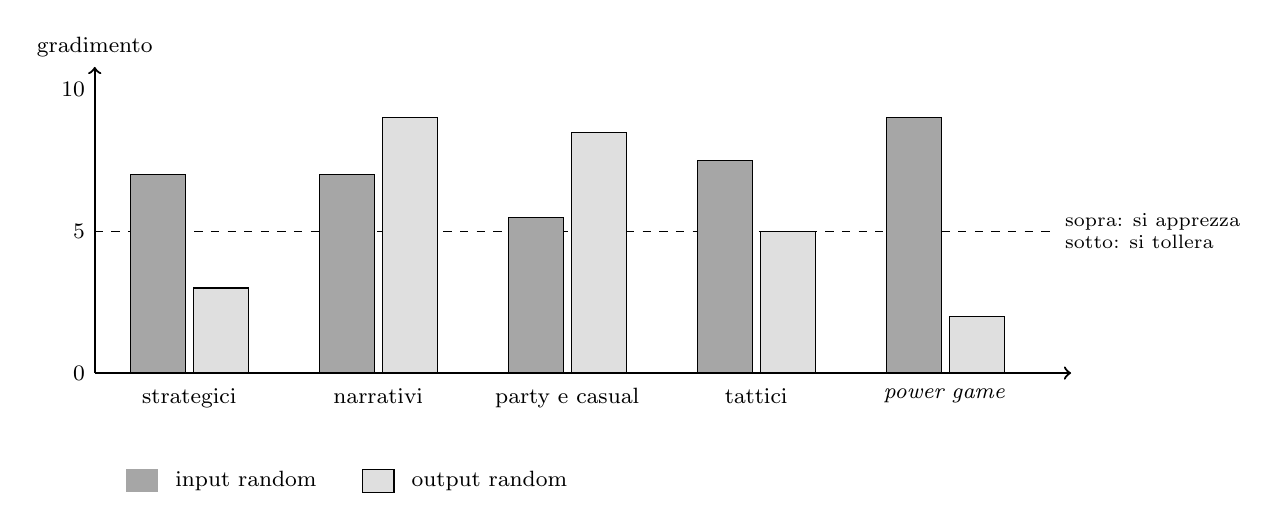
\begin{tikzpicture}[font=\small, x=1.0cm, y=0.36cm]
  \draw[thick, ->] (0,0) -- (12.4,0);
  \draw[thick, ->] (0,0) -- (0,10.8) node[above, font=\footnotesize] {gradimento};
  \foreach \y in {0,5,10} \node[left, font=\footnotesize] at (0,\y) {\y};
  \draw[dashed] (0,5) -- (12.2,5) node[right, font=\scriptsize, align=left]
    {sopra: si apprezza\\sotto: si tollera};
  \foreach \x/\lab/\i/\o in {1.2/strategici/7/3, 3.6/narrativi/7/9, 6.0/party e
      casual/5.5/8.5, 8.4/tattici/7.5/5, 10.8/\emph{power game}/9/2} {
    \fill[gray!70] (\x-0.75,0) rectangle (\x-0.05,\i);
    \fill[gray!25] (\x+0.05,0) rectangle (\x+0.75,\o);
    \draw (\x-0.75,0) rectangle (\x-0.05,\i);
    \draw (\x+0.05,0) rectangle (\x+0.75,\o);
    \node[below, font=\footnotesize, align=center, text width=2.2cm] at (\x,-0.2) {\lab};
  }
  \fill[gray!70] (0.4,-4.2) rectangle (0.8,-3.4);
  \node[anchor=west, font=\footnotesize] at (0.9,-3.8) {input random};
  \fill[gray!25] (3.4,-4.2) rectangle (3.8,-3.4); \draw (3.4,-4.2) rectangle (3.8,-3.4);
  \node[anchor=west, font=\footnotesize] at (3.9,-3.8) {output random};
\end{tikzpicture}
\caption{Quanto le cinque famiglie di giocatori della slide di Diego gradiscono l'input e
l'output random, su una scala con 5 come valore medio. \textbf{I valori sono indicativi}: la
trascrizione riporta solo i giudizi a voce (``apprezzano'', ``tollerano'', ``disapprezzato
ancora più dei tattici''), non i numeri della slide; il grafico ne rende l'ordine e il segno.}
\label{a15:fig:pubblico}
\end{figure}

\paragraph{Le sottocategorie.} Certo, per ogni famiglia ci sono molte sottocategorie: nei
giochi strategici, i giochi a carte, a turni, a \emph{round}, cooperativi. ``Il mondo qui è
molto più vasto.''

\subsection{La ricerca: leggere le recensioni}

Come si fa a sapere che cosa vuole il proprio pubblico? \textbf{Facendo ricerca}. Diego mostra
come: si sceglie il proprio gioco di riferimento, per esempio \textbf{\emph{Wingspan}}, e si
leggono i commenti, ``14.000 commenti, non tutti ovviamente''. Si cerca di capire perché certe
persone gli danno 9, perché qualcuno gli dà 8, che è un buon voto.
\begin{itemize}
  \item Chi gli dà un voto alto cita \textbf{la varietà delle strategie}: già questo dice che
        \emph{Wingspan} rientra nei giochi strategici. Lo stesso utente lo chiama ``un
        \emph{multiplayer solitaire}'', ma non in senso negativo.
  \item Chi gli dà un voto basso scrive che è un gioco ``bellissimo da vedere'' ma
        \textbf{\emph{themeless}}, senza tema: si gioca, è bello a vedersi, ma si gioca poco.
  \item Altri lo descrivono come un \textbf{\emph{engine building}}: quindi ha anche
        caratteristiche da \emph{power game}, perché si basa sul costruire un motore di
        successo. Uno nota che il risultato dipende molto dalle carte della mano iniziale; uno
        lo trova un gioco \emph{casual} che però richiede parecchio tempo.
  \item Un altro scrive che il gioco non è gratificante soprattutto perché \textbf{il tema non è
        integrato con le meccaniche}, e che è come giocare ``con l'attrito'' tra tema e
        regole\footnote{Le recensioni sono lette a voce in inglese e la trascrizione le rende
        in modo approssimativo; il capitolo ne riporta il senso.}.
\end{itemize}

\paragraph{Che cosa se ne ricava.} Qui si torna a ciò che si è detto: \textbf{l'output
funziona soprattutto con elementi narrativi e tematici}, nei giochi ad alta tematicità. Se si
dovesse fare un concorrente di \emph{Wingspan}, l'output random potrebbe essere interessante,
ma \textbf{in piccole dosi}, perché i giochi strategici hanno giusto una tolleranza per
l'output. Magari un solo momento specifico; e se avviene, deve avvenire \textbf{perché è legato
al tema}, altrimenti non dovrebbe avvenire affatto. ``Ovviamente questa non è una ricerca'', ma
è da questi punti che si costruiscono i dettagli alla base di una ricerca.

% ---------------------------------------------------------------------
\section{Il \emph{cheat sheet} del random}
\label{a15:sec:cheatsheet}

L'ultima slide è ``un piccolo \emph{cheat sheet} del random'': una tabella con le diverse
\textbf{dimensioni} e, per ciascuna, il comportamento di input, output e combinato. Diego
pensava di non leggerla tutta, ``ma ce l'abbiamo il tempo: approfittiamo''
(tabella~\ref{a15:tab:cheatsheet}). Qualche nota sulle voci.

\paragraph{Tempo e \emph{agency}.} L'input avviene \textbf{prima} della fase decisionale,
l'output \textbf{dopo}, il combinato \textbf{prima e dopo}. Con l'input, l'\emph{agency} del
giocatore è \textbf{la risposta all'incertezza}; con l'output è media o bassa, perché il caso
``copre'' la decisione (``posso volerti attaccare, poi il dado mi dice che non ti ho
attaccato''): meglio ridurlo, non annullare la decisione del giocatore ma ridurne l'efficacia.

\paragraph{Profondità, tono, ruolo.} L'input ha una profondità strategica \textbf{alta},
perché promuove pianificazione e adattamento; l'output media, perché non si vuole cancellare la
situazione strategica. Il tono emotivo: \textbf{\emph{puzzle} e logica} per l'input,
\textbf{dramma e tensione} per l'output, \textbf{caos} per il combinato, ``perché tutto può
capitare''. Nel gioco di ruolo l'input è molto presente, perché spesso è il master a darlo
(``arriva un tizio e ti dà un pugno in faccia''); l'output è medio, di nuovo per ridurre
l'efficacia dell'azione senza annullare il giocatore.

\paragraph{Tipi di gioco e attrito.} Input: \emph{eurogame}, \emph{deck builder},
\emph{engine building}. Output: \emph{party game}, giochi di ruolo e di combattimento, e gli
``\emph{American trash}''\footnote{Il termine corrente è \emph{Ameritrash}: i giochi
``all'americana'', molto tematici e con molto caso, contrapposti agli \emph{eurogame}.} come
\emph{Exploding Kittens} e \emph{Unstable Unicorns}, dove ``trash'' non è negativo: indica alto
fattore comico, alto fattore \emph{party}, basso fattore di gioco. Quanto all'\textbf{attrito
con la strategia} (\emph{friction}): nell'input è basso, perché se si sta già rendendo meno
efficace il giocatore non gli si vuole dare un problema in più; \textbf{l'output è proprio dove
l'attrito avviene}: invece di tre danni, ne hai fatti due.

\paragraph{Mitigazione, frustrazione, equità.} Le mitigazioni tipiche: per l'input il
\textbf{\emph{draft}} (ho più carte e ne scelgo una), il \textbf{\emph{cycling}} (una carta
diventa un'altra carta) e il \textbf{\emph{setup} controllato}; per l'output \emph{reroll},
modificatori e pagare risorse per ottenere vantaggi; per il combinato il \textbf{\emph{deck
shaping}} (nei formati ``eterni'' di \emph{Magic} il mazzo è randomico, ma è talmente
ottimizzato che in realtà non lo è), il \emph{push your luck} e il controllo delle risorse.
Il \textbf{rischio di frustrazione} è minimo con l'input, che i giocatori vedono come
un'occasione per mostrare la propria competenza; con l'output c'è se si cancellano le azioni
dei giocatori, meno se le si mitiga; con il combinato è altissimo: ``se è tutto caso, non sento
neanche che sto giocando''. L'\textbf{equità percepita} è alta con l'input (vedo le
informazioni e poi decido), molto bassa con l'output, soprattutto se la decisione viene
cancellata; con il combinato, paradossalmente, \textbf{è percepita meglio}: se tutto è casuale,
lo si accetta. ``Ti piace la pizza? Qui fanno solo pizza. Allora è andata così.''

\paragraph{Giocatore ideale, complessità, temi.} Input: pensatori, ottimizzatori,
pianificatori; output: \emph{casual}, \emph{thrill seeker}, giocatori sociali; combinato: chi
è guidato dalla storia, i ``caotici''. La complessità è \textbf{alta} con l'input (in base a
come si costruisce e si riceve, si possono prendere decisioni strategiche e tattiche),
\textbf{bassa} con l'output (che non aggiunge complessità, riduce l'efficacia), \textbf{media}
con il combinato, che però può diventare estremamente complesso (``è randomico qui, è
randomico là, è randomico su, è randomico giù''). I temi: astratti, economia e logica per
l'input; combattimento, \emph{gambling} e tensione per l'output; mondi caotici, pericolo e
imprevedibilità per il combinato.

\begin{table}[htbp]
\centering
\footnotesize
\begin{tabular}{@{}>{\raggedright\arraybackslash}p{2.3cm}>{\raggedright\arraybackslash}p{3.7cm}>{\raggedright\arraybackslash}p{3.7cm}>{\raggedright\arraybackslash}p{3.7cm}@{}}
\toprule
\textbf{Dimensione} & \textbf{Input} & \textbf{Output} & \textbf{Combinato} \\
\midrule
Tempo & prima della decisione & dopo la decisione & prima e dopo \\
\addlinespace
\emph{Agency} & alta: risposta all'incertezza & media o bassa: il caso copre la decisione &
  --- \\
\addlinespace
Profondità strategica & alta: pianificare e adattarsi & media: non cancellare la strategia
  & --- \\
\addlinespace
Tono emotivo & \emph{puzzle}, logica & dramma, tensione & caos \\
\addlinespace
Gioco di ruolo & molto presente (il master) & medio & --- \\
\addlinespace
Tipi di gioco & \emph{eurogame}, \emph{deck builder}, \emph{engine building} & \emph{party},
  GdR, combattimento, \emph{Ameritrash} & --- \\
\addlinespace
Attrito con la strategia & basso & è qui che avviene & --- \\
\addlinespace
Mitigazione tipica & \emph{draft}, \emph{cycling}, \emph{setup} controllato & \emph{reroll},
  modificatori, pagare risorse & \emph{deck shaping}, \emph{push your luck}, controllo delle
  risorse \\
\addlinespace
Rischio di frustrazione & basso & alto se cancella, minore se mitiga & altissimo \\
\addlinespace
Esempi & \emph{Dominion}, \emph{Terraforming Mars}, \emph{Race for the Galaxy} & \emph{King
  of Tokyo}, Risiko, D\&D, ``Headside''\protect\footnotemark & \emph{Hearthstone},
  \emph{Gloomhaven}, \emph{Sleeping Gods}, \emph{Clank!} \\
\addlinespace
Equità percepita & alta & molto bassa & sorprendentemente buona \\
\addlinespace
Giocatore ideale & pensatori, ottimizzatori, pianificatori & \emph{casual}, \emph{thrill
  seeker}, sociali & guidati dalla storia, caotici \\
\addlinespace
Complessità & alta & bassa & media (può esplodere) \\
\addlinespace
Temi & astratti, economia, logica & combattimento, \emph{gambling}, tensione & mondi caotici,
  pericolo, imprevedibilità \\
\bottomrule
\end{tabular}
\caption{Il \emph{cheat sheet} del random, ricostruito da ciò che Diego legge a voce. I
trattini indicano le caselle che non legge, o che la trascrizione non restituisce.}
\label{a15:tab:cheatsheet}
\end{table}
\footnotetext{Così nella trascrizione; il titolo non è ricostruibile.}

Con questo, ``siamo stati perfetti'' (``51'', dice Diego guardando l'orologio): la lezione è
finita.

% ---------------------------------------------------------------------
\section{Le domande e la chiusura}
\label{a15:sec:chiusura}

Diego prova a caricare le slide nella chat di Zoom, ma non ci riesce (``probabilmente non mi
hanno dato i diritti''): le passerà a Daniele, che le girerà agli studenti, e ad
Agnese\footnote{Il nome compare solo qui; dal contesto è una persona dell'accademia che
gestisce i materiali del corso.} per chi non ha potuto seguire in diretta.

\paragraph{La domanda di Oksana: da dove vengono i dati?} Oksana chiede dove si prendono le
statistiche come quelle sulla tolleranza delle diverse categorie, della penultima slide.
``Ottima domanda.'' Esistono siti che \textbf{aggregano} queste informazioni: \textbf{Quantic
Foundry}\footnote{Quantic Foundry è una società di ricerca sulle motivazioni dei giocatori,
nota per il suo modello di motivazioni e per i questionari pubblici, anche per i giochi da
tavolo.} e \textbf{BoardGameGeek}\footnote{Nella trascrizione ``Board Game Geek'' e
``Burgundy''.}; e anche su \textbf{Reddit} si fanno costantemente ricerche del genere. Gli
altri due modi:
\begin{itemize}
  \item \textbf{analizzare da sé}, come si è fatto con \emph{Wingspan}: guardare giochi di
        categoria simile e che cosa la gente ne apprezza e no;
  \item \textbf{fare la propria ricerca} con un \emph{survey}, un questionario, da proporre
        sulla pagina BoardGameGeek o sul \emph{subreddit} del gioco di riferimento.
\end{itemize}
Esistono anche siti a pagamento, ma Diego non li consiglia: i loro dati sono ``gli stessi
vostri'', semplicemente già accumulati e aggregati nel tempo. ``Molto spesso non ne vale la
pena.''

\paragraph{Un commento sui \emph{dice forge}.} Uno studente dice che la lezione è stata
chiara e molto utile per il \emph{project work}: durante la lezione gli sono venute in mente un
paio di cose da provare, soprattutto in \emph{playtest}. E consiglia, a proposito dei giochi
con dadi da costruire, un gioco per telefono ``vecchiotto, molto carino'', che la trascrizione
chiama ``Diceyros''\footnote{Il titolo non è ricostruibile.}. Per Diego i \emph{dice forge}
sono ormai diventati \textbf{un genere}: si ha il random, ma \textbf{si forgia il proprio
random}. ``È una di quelle cose che, con il senno di poi, io come designer posso solo dire:
\emph{wow}, ha senso''; ma avere l'idea per primi ``non è per nulla facile''.

\paragraph{Lo spazio creativo del random.} Diego ne è convinto, ``è una mia opinione, ma ne
sono convinto'': c'è \textbf{ancora tantissimo spazio creativo nel random}, nei giochi da
tavolo e nei videogiochi, sia nel come integrarlo sia nel come usarlo. Per molti anni i
designer sono stati limitati ai \textbf{D6 e ai D20}, per ragioni produttive: fare i dadi
costava, e se si chiedeva a un produttore un dado da 13 ti diceva ``quanti ne vuoi? mille? sono
centomila euro'', perché serviva un macchinario apposta, e si finiva a usare il D12 o il D10
standard. Oggi \textbf{fare i dadi non costa più}: se si vuole un gioco con un D13, o due D13,
perché si è calcolata la curva a campana che serve, ``si fa''. E poi c'è il
\textbf{digitale}: con un'app si può rendere casuale quasi tutto (la posizione, l'età dei
giocatori, le chiamate\ldots), cose che prima non c'erano.

\paragraph{\emph{Atmosfear}.} L'ultimo esempio è un gioco che Diego ha sempre adorato e che
giocava da bambino, ``per questo dicevo che molti di voi non lo conosceranno'' (``Oksana, secondo
me, lo conosce''): \textbf{\emph{Atmosfear}}\footnote{Nella trascrizione ``Atmosphere''. È il
gioco da tavolo con videocassetta uscito all'inizio degli anni Novanta (in origine
\emph{Nightmare}), con il Guardiano delle chiavi (\emph{Gatekeeper}).}. Si giocava con
\textbf{una videocassetta sul televisore}: in base a ciò che succedeva sul tabellone si doveva
reagire in certi momenti, e il personaggio sullo schermo, il \textbf{Guardiano}, si rivolgeva
ai giocatori. Diego fa sentire uno spezzone: tutti i giocatori sono marchiati con un colore e
un numero; quando il Guardiano li chiama, devono rispondere ``\emph{Yes, my Gatekeeper!}''; se
non rispondono in tempo, vengono puniti e mandati nel buco nero più vicino, e non giocano
finché lui non lo decide; il Guardiano chiama all'improvviso un numero, ``\emph{the one who
holds the lowest number}'', e ci sono timer, chiavi da vincere e da perdere. Uno studente
osserva che ricorda un po' i principi dei \emph{party game} con app\footnote{Nella trascrizione
``il principio di righe game'': il riferimento non è ricostruibile.}. ``Esatto.''

\paragraph{Il valore del limite.} \emph{Atmosfear} era ``molto particolare e unico, per quanto
limitato'': c'era il televisore, c'erano dei vincoli. Ma per esempio garantiva che la partita
durasse \textbf{circa un'ora e dieci}, perché finiva quando finiva la registrazione. ``Anche se
non vi sembra, c'è veramente tantissimo spazio creativo nel random.'' Diego saluta, le slide
arriveranno tramite Daniele, ``buona serata, grazie mille''.

% ---------------------------------------------------------------------
\section*{Punti chiave del capitolo}
\addcontentsline{toc}{section}{Punti chiave del capitolo}

\begin{itemize}
  \item ``Random'' ha sei ingredienti: mancanza di \emph{pattern} (vera o percepita, quindi
        relativa al \emph{target}), assenza di decisione conscia (togliere decisioni rende
        un'azione random o ingiusta), il caso contro il piano, l'assenza di causa o di
        intenzione, la possibilità statistica, il pericolo e il risultato incerto.
  \item Le probabilità si calcolano in due modi: \textbf{moltiplicando} (eventi indipendenti
        si moltiplicano, non si sommano) o \textbf{disegnando l'albero}, che mostra anche
        quanto si espande lo spazio delle scelte.
  \item Tre tipi di random: \textbf{vero} (dadi, monete), \textbf{pseudo-random} (i computer:
        individuabile e sfruttabile, come i \emph{seed}) e \textbf{controllato}: la somma di più
        elementi casuali segue la curva a campana, e conoscerla è ``l'arma segreta'' del
        designer (il ladro di \emph{Catan} sul 7).
  \item Il caso entra in tre momenti: \textbf{input} (prima della decisione), \textbf{output}
        (dopo), \textbf{combinato} (entrambi nella stessa decisione): nove combinazioni con i
        tre tipi.
  \item \textbf{Input}: carte, ruoli, \emph{setup}. Dà decisioni tattiche, rigiocabilità
        (\emph{Cosmic Encounter}) e livella le abilità; rischia la \emph{turn one win}, la
        paralisi da analisi, la falsa strategia e, se controllato troppo, la prevedibilità
        (la briscola). Nasce input e finisce controllato; deve far sentire il giocatore più
        potente senza togliergli l'\emph{agency}.
  \item Cento partite: se la fortuna decide il 30\% o più delle vittorie è troppa; l'obiettivo
        è circa il 20\%. E \textbf{l'interessante batte il giusto}: se è sbilanciato, si
        aggiunge una regola (le debolezze di \emph{Arkham}, il \emph{mulligan}).
  \item \textbf{Output}: il caso sul successo o sull'entità del risultato. Serve al
        \textbf{dramma} (\emph{Affari tuoi}, \emph{Golden Balls}), all'alto rischio con alta
        ricompensa e a livellare le abilità; la troppa sfortuna toglie \emph{agency}. Poco
        all'inizio, di più verso la fine, senza annullare ciò che è avvenuto prima.
  \item Mitigare l'output: \emph{reroll}, modificatori, assicurazioni, successo nel
        fallimento (con piccoli bonus, per evitare lo stallo). Usarlo per il dramma, non per
        ogni decisione; mitigazione limitata (cinque \emph{reroll} a partita); legarlo al tema
        e alla scelta del giocatore (il dado critico). In negativo: \emph{Killer Bunnies}.
  \item L'output funziona nei giochi tematici, \emph{casual} e di \emph{risk management}; il
        gioco dell'oca piace ai bambini perché credono che il 6 sia merito loro.
  \item \textbf{Combinato}: pericoloso perché toglie potere decisionale, ma apre il
        \emph{problem solving} creativo (le maledizioni di \emph{Magic}; il gioco di dadi che
        con un input nascosto passa da statistico a bluff), la profondità strategica
        (Atlantide nel Risiko contro lo stallo) e la narrativa (\emph{Pasión de las Pasiones}).
  \item Mitigare il combinato: \emph{reroll}, modificatori, \textbf{\emph{push your luck}} (il
        secondo random è una scelta), \textbf{sistemi ibridi} (la Scoperta di
        \emph{Hearthstone}), random controllato (il boomerang dei due dadi),
        \textbf{progressione} (\emph{Dice Forge}). Evitare l'\textbf{effetto valanga} con le
        \textbf{fasi} (\emph{L'eredità}).
  \item I pubblici tollerano il caso in modo diverso: strategici e \emph{power game} amano
        l'input e non l'output; narrativi e \emph{party} amano l'output. Lo si scopre facendo
        ricerca: recensioni (\emph{Wingspan}), Quantic Foundry, BoardGameGeek, Reddit,
        questionari propri.
  \item Il \emph{cheat sheet}: input = logica, alta \emph{agency}, alta complessità, bassa
        frustrazione; output = dramma, attrito, alta frustrazione se cancella; combinato =
        caos, frustrazione altissima, ma equità percepita sorprendentemente buona.
  \item C'è ancora molto spazio creativo nel random: dadi su misura (un D13 oggi si fa), app,
        e idee come \emph{Atmosfear}.
\end{itemize}

%
%  Tutte le etichette di questo capitolo hanno il prefisso "a15:"
%  (a15:cap:..., a15:sec:..., a15:fig:..., a15:tab:...). Il capitolo è
%  autonomo: non contiene \ref verso altri capitoli.
%  Le figure e le tabelle sono ricostruzioni schematiche di quanto
%  detto a voce e mostrato nelle slide (che non sono nella
%  trascrizione), non copie delle slide. Dove la trascrizione è troppo
%  rovinata per ricostruire un dettaglio (un nome, un titolo, un
%  numero), il capitolo lo dice invece di inventarlo; dove Diego dà un
%  numero o un fatto che non torna, il capitolo lo riporta come detto e
%  lo corregge in nota.
% =====================================================================

\chapter[Il random nel game design]{Il random nel game design: input, output e casualità
combinata}
\label{a15:cap:random}

Questa è la \textbf{quindicesima lezione} del corso di \textbf{Analog Game Design}, ed è
la lezione sull'\textbf{RNG}, la casualità nei giochi, annunciata fin dal primo giorno e
spostata più volte nel calendario. La tiene \textbf{Diego Ricchiuti}, direttore del corso
di Game Design dell'accademia e \emph{game designer} con una lunga carriera nei videogiochi
e qualche incursione nei giochi da tavolo. Daniele, presentandolo, promette una lezione
``più proprio di \emph{design} vero e proprio tecnico'': che cos'è l'RNG e come lo si usa
nel \emph{system design}.

Diego costruisce la lezione come ama fare, ``a partire dalle definizioni''. Prima si chiede
che cosa intendiamo davvero quando diciamo che una cosa è ``random'', e ne ricava sei
ingredienti; poi mostra come si calcola una probabilità, distingue \textbf{tre tipi di
random} (vero, pseudo-random e controllato) e li incrocia con \textbf{tre momenti} in cui la
casualità può entrare in una decisione: \textbf{prima} (l'\emph{input random}),
\textbf{dopo} (l'\emph{output random}) o \textbf{entrambi} (il random \textbf{combinato}).
A ciascuno dei tre momenti dedica un blocco della lezione, con la stessa struttura: che
cos'è, perché lo si usa, quali rischi porta, come lo si mitiga, dove funziona meglio, e
qualche consiglio ``da persona che fa questa roba da tanti anni''. La lezione si chiude con
il rapporto tra casualità e \textbf{pubblico}, con una tabella riassuntiva (un ``piccolo
\emph{cheat sheet} del random'') e con le domande degli studenti.

Il filo che lega tutto è un'idea che Diego ripete in più forme: il random non è un nemico
del \emph{design}, ma il suo strumento più potente, \textbf{a patto di controllarlo}. Il
\textbf{random controllato}, cioè sapere che cosa è statisticamente più probabile e
costruirci sopra le regole, è ``l'arma segreta di noi designer''; e la casualità va dosata
in modo che il giocatore si senta \textbf{più potente} e non privato della propria
\emph{agency}. Lo dice anche in negativo: ``con il random, favorite l'\emph{interessante}
invece del \emph{giusto}''.

\paragraph{Data, formato, persone.} La lezione è \textbf{online}, su Zoom, e dura le
``classiche tre ore'' con una pausa a metà; inizia alle 17, con il solito quarto d'ora di
attesa per i ritardatari. La data non è mai detta, e diversi indizi fanno pensare che la
trascrizione \textbf{non} venga da una lezione dal vivo dell'edizione in corso, ma sia la
\textbf{registrazione della lezione sull'RNG di un'edizione precedente} del corso,
presumibilmente la prima\footnote{Nel calendario ripassato da Ruggero nella lezione su
Tabletop Simulator la lezione di Diego sull'RNG era fissata al 6 novembre, ed era poi stata
sostituita dalla lezione sul \emph{playtest}; nessun capitolo successivo la ricolloca. In
questa trascrizione, invece: gli studenti presenti hanno nomi che non compaiono mai nei
capitoli precedenti (Mauro, Andrea, Alessandro, Davide, Giuseppe, un altro Diego, Federico,
Daniele, Oksana, Jacopo); Daniele dice che i gruppi stanno realizzando un prototipo ``che ci
porteranno attorno ai primi di luglio'' e che verrà finalizzato ``attorno al 20 di
settembre''; ricorda un tutoraggio ``a inizio luglio''; e durante la pausa Diego dice di
``morire di caldo'' e parla di ventilatori e deumidificatori. Tutto fa pensare a una lezione
tenuta a inizio estate, durante un'edizione precedente (con ogni probabilità quella del
2025, ``l'anno scorso'' di cui parlano i docenti nella prima lezione). Il capitolo non
assegna una data e tratta la lezione come una registrazione messa a disposizione del corso.
Anche l'ordine (dopo le due lezioni di Marta) è quello in cui la trascrizione è stata
fornita, non necessariamente quello in cui la lezione è stata vista.}.
All'inizio c'è \textbf{Daniele}, il docente titolare, che deve tornare dopo pochi minuti
``dagli altri di \emph{Narrative}'', un altro corso in cui deve prendere le presenze. Fa
l'appello: risultano presenti, o in arrivo, \textbf{Mauro}, \textbf{Andrea},
\textbf{Davide} (che conosce già Diego e ``alcune cose le sa già''), \textbf{Diego} (uno
studente omonimo del docente), \textbf{Federico}, \textbf{Oksana} e
\textbf{Jacopo}\footnote{La trascrizione scrive anche ``Giacopo'' e ``Iacomo''. Nell'appello
compare anche un ``Fabris'' (o ``Fabrizio''?) che non si sente più; più avanti Diego dice che
Fabrizio è il nome di suo fratello, ma è un'altra cosa.}; \textbf{Giuseppe} segue in
differita dalla registrazione; \textbf{Alessandro} ha avvisato che non ci sarà;
di \textbf{Daniele} (uno studente) non si sa nulla. Intervengono a voce soprattutto
\textbf{Jacopo}, \textbf{Davide}, \textbf{Andrea} e, alla fine, \textbf{Oksana}.

\paragraph{Avvertenze di lettura.} Le stesse dei capitoli precedenti. La trascrizione è
automatica e storpia molti nomi: \emph{Hearthstone} è ``Airstone'', \emph{Sleeping Gods}
è ``Sleeping Garden'' o ``Sleeping God'', \emph{Clank!} è ``Crank'', \emph{Dice Forge} è
``Forge Dice'', \emph{Among Us} è ``da Mongas'', \emph{Atmosfear} è ``Atmosphere'', il
Texas Hold'em è ``Texas Olden'', \emph{The Settlers of Catan} è ``Settles of Catan'' o ``7
Socratan'', \emph{Pachinko} è ``pacinco'', la Kamčatka del Risiko è ``Kamciak'',
``canciacca'' e ``cranciacca''. Dove la ricostruzione è sicura, o molto probabile, il
capitolo usa la forma corretta e lo segnala in nota la prima volta; dove non lo è,
riporta la forma della trascrizione e lo dice. La trascrizione \textbf{si apre e copre
l'intera pausa con frasi senza senso ripetute in ciclo} (``la situazione è questa, la
migliore dal 2005'', ``il numero di persone è molto più basso dopo il raggio di persone'',
``la struttura del giardino''), che il capitolo ignora; e \textbf{in un punto della parte
sull'output random} una stringa ripetuta (``Output transcript'') copre una parte della
spiegazione, che il capitolo ricostruisce per quanto possibile e segnala. Diego, infine,
parla a braccio e dà qualche numero o fatto che non torna (la percentuale del 7 con due
dadi, l'origine del nome della curva a campana, il numero di tessere di
\emph{Carcassonne}, gli alieni di \emph{Cosmic Encounter}, l'età del \emph{London
mulligan}): il capitolo riporta ciò che ha detto e, in nota, i dati corretti.

\paragraph{Come leggere questo capitolo.} Il capitolo segue l'ordine della lezione. Le
figure ricostruiscono gli schemi che emergono dal discorso o che Diego disegna a mano
durante la lezione (l'albero delle monete, le distribuzioni dei dadi, il momento della
casualità rispetto alla decisione, le curve di input, output e tensione, la tolleranza dei
diversi pubblici); le tabelle riassumono le definizioni, le nove combinazioni, i pro e i
rischi di ciascun tipo di random, le tecniche di mitigazione e il \emph{cheat sheet}
finale. Qua e là, dei paragrafi di \textbf{approfondimento} collegano la lezione ai libri
di game design di riferimento (soprattutto \emph{The Art of Game Design} di Jesse Schell e
\emph{Challenges for Game Designers} di Brenda Brathwaite e Ian Schreiber), e qualche
piccolo calcolo verifica gli esempi numerici di Diego; sono segnalati come tali e non
fanno parte della lezione.

Il percorso del capitolo:
\begin{enumerate}
  \item l'apertura con Daniele e la presentazione di Diego (sezioni
        \ref{a15:sec:apertura} e~\ref{a15:sec:diego});
  \item che cos'è il random: le definizioni, il calcolo delle probabilità, i tre tipi
        di random e le nove combinazioni (sezioni
        \ref{a15:sec:definizioni}--\ref{a15:sec:nove});
  \item l'input random (sezione~\ref{a15:sec:input});
  \item l'output random (sezione~\ref{a15:sec:output});
  \item dopo la pausa, il random combinato e la sua mitigazione (sezioni
        \ref{a15:sec:combinato} e~\ref{a15:sec:mitigazionecomb});
  \item il pubblico, il tema e il \emph{cheat sheet} (sezioni \ref{a15:sec:pubblico}
        e~\ref{a15:sec:cheatsheet});
  \item le domande e la chiusura (sezione~\ref{a15:sec:chiusura}).
\end{enumerate}

% ---------------------------------------------------------------------
\section{L'apertura: Daniele presenta Diego}
\label{a15:sec:apertura}

I primi minuti sono di attesa e di chiacchiere. Daniele e Diego si conoscono bene, e
parlano della nuova foto del profilo LinkedIn di Diego (``la foto grande'', dice Daniele,
``è veramente carina''); Diego osserva che quando si è a un evento professionale con un
fotografo professionista ``si nota la differenza'', e che lui tiene ``una foto fatta bene
all'anno''. Davide conosce già Diego, che ha avuto come docente ``quattro anni fa'': per lui
la parte iniziale in cui Diego si presenta sarà uno \emph{spoiler}, ma ``un ripasso fa
sempre bene''. Si aspetta, come di consueto, fino alle cinque e un quarto. Tra una cosa e
l'altra, Daniele dice che ha seguito una conferenza stampa che lo ha molto emozionato:
questa parte della trascrizione è però quasi del tutto incomprensibile\footnote{``Io ho
partecipato a questa conferenza stampa, sono stato molto emotivo [\ldots] sono stati forzati
a dare la mia mano a questo giovane iconore'': il contenuto non è ricostruibile, ed è
probabilmente in parte rumore della trascrizione automatica.}.

\paragraph{Che cosa sta facendo il corso.} Daniele spiega a Diego che la lezione è ``la
classica da tre ore con la pausa'' e che, se vuole, può passargli le slide da caricare sul
\emph{drive} condiviso degli studenti. I gruppi stanno già realizzando un prototipo di gioco
analogico, che porteranno ``attorno ai primi di luglio'' e finalizzeranno per presentarlo
``attorno al 20 di settembre''; dopo quella data, se Diego vuole, potrà vederli anche lui.
Diego accetta volentieri.

\paragraph{La presentazione.} Daniele lascia subito la parola, perché deve tornare
``dai ragazzi di \emph{Narrative}'' (``e quando lasci da soli i topi ballano''). Presenta
Diego come \textbf{direttore del corso di Game Design} dell'accademia\footnote{Nella
trascrizione ``ad Ive'' e, poco dopo, ``qui a Dive'' e ``il Discord di Hive'': è con ogni
probabilità l'accademia stessa (AIV), che i capitoli precedenti chiamano semplicemente
``l'accademia''.} e ``grande esperto di game design, sia videoludico che \emph{tabletop}'',
a cui è stata chiesta una lezione ``specificatamente su RNG'': che cos'è, un po' di
\emph{system design}, ``qualcosa più proprio di \emph{design} vero e proprio tecnico''.

\paragraph{Il calendario.} Daniele ricorda che ci si rivede \textbf{lunedì}, con lui e
``forse anche Ruggero'', per la lezione sul \textbf{\emph{world building}}\footnote{Nella
trascrizione ``War Building'': dal contesto è il \emph{world building}.}; le altre lezioni
seguiranno il calendario, con ``piccoli cambiamenti'' sempre pensati per dare agli studenti i
temi più utili al corso. A inizio luglio ci sarà un altro tutoraggio\footnote{Con ``Meo
Corrugge'', secondo la trascrizione: potrebbe essere una storpiatura di ``Ruggero'', ma il
nome non è ricostruibile con certezza.}; il calendario completo è online.

\paragraph{Le registrazioni e l'Help Desk.} Prima di uscire, Daniele risponde ad Andrea, che
da quel giorno non riesce più a rivedere le registrazioni delle lezioni sul sito (``questo
video è inesistente'', su tutti i video). Probabilmente, dice Daniele, è ``crollato il
server'' dove stanno i video. E dà un'indicazione che vale per tutti: per i \textbf{problemi
tecnici} c'è, in alto nel Discord dell'accademia, un canale apposito chiamato \textbf{Help
Desk}; lì si scrive ``sono studente di questo corso e vi segnalo questo problema'', e
rispondono direttamente i tecnici.

% ---------------------------------------------------------------------
\section{Chi è Diego}
\label{a15:sec:diego}

Diego condivide lo schermo, chiede conferma che le slide si vedano e comincia con una
``brevissima presentazione''. Lo si può trovare su \textbf{LinkedIn}, dove gli si possono
fare domande anche dopo la lezione: ``è tutto per me soltanto un piacere''. Oltre a
dirigere il corso di Game Design dell'accademia, elenca i progetti a cui ha lavorato:
\begin{itemize}
  \item \textbf{\emph{Tom Clancy's Ghost Recon Wildlands}}, come \emph{lead
        designer}\footnote{Così nella trascrizione. Il capitolo riporta i ruoli come detti a
        voce, senza verificarli.};
  \item un titolo che la trascrizione riporta come ``\emph{Konaka Madness}''\footnote{Il
        titolo non è ricostruibile.};
  \item ``\emph{Donai}'', che definisce ``il primo \emph{donation game} al
        mondo''\footnote{Il nome è riportato come nella trascrizione e non è
        verificabile.};
  \item \textbf{\emph{Dying Light 2}}, come \emph{lead designer};
  \item \textbf{\emph{Enotria}}\footnote{Con ogni probabilità \emph{Enotria: The Last Song},
        \emph{soulslike} di ambientazione italiana.}, come consulente;
  \item \textbf{\emph{A Quiet Place}}\footnote{Con ogni probabilità \emph{A Quiet Place: The
        Road Ahead}, il videogioco tratto dalla serie di film.}, come \emph{creative
        director};
  \item un gioco uscito ``letteralmente due settimane fa'', di cui è \emph{design director},
        che la trascrizione riporta come ``\emph{Star of the Drag}''\footnote{Il titolo non è
        ricostruibile; ``su Ovunque'' significa forse che è uscito su tutte le piattaforme.}.
\end{itemize}
Ha scritto anche \textbf{un libro di game design}, e dice di essere ``l'unico italiano nella
storia ad averlo fatto''\footnote{Così nella trascrizione: il senso è con ogni probabilità
che sia l'unico italiano ad aver scritto un libro di game design di quel tipo, o per
quell'editore; il titolo non viene detto.}, e un secondo libro, che invece riguarda il
\textbf{\emph{business} dei videogiochi} (trovare fondi, lavorare con i \emph{publisher}),
scritto insieme a un caro amico, \emph{business developer}, che la trascrizione chiama
``John Henley''\footnote{La grafia del nome non è verificabile.}.

\paragraph{I giochi da tavolo.} Ha lavorato anche sui giochi analogici. Il suo primo gioco
da tavolo è \textbf{\emph{Artonauti -- Il mosaico del tempo}}, realizzato per il marchio
\textbf{Artonauti}\footnote{Nella trascrizione ``Artonauti'' e, più avanti, ``attornato''.
Artonauti è un marchio editoriale italiano per ragazzi, legato a un album di figurine sulla
storia dell'arte.}: un \textbf{\emph{family game}} per bambini tra i 6 e gli 11--12 anni e i
loro genitori. Per lo stesso marchio ha fatto le \textbf{\emph{Elemental Cards}}: carte
divise nei quattro elementi classici (fuoco, terra, acqua, aria), con valori e abilità, per
poterci costruire sopra ``un gioco, fondamentalmente''.

\paragraph{Perché raccontarlo.} Non per vanto, ma ``per dirvi che se sono qui a parlarvi di
questi argomenti, è perché so di cosa sto parlando''. Fa videogiochi, e giochi in generale,
da \textbf{16 anni}, e ne ha viste ``di tutti i tipi'': dal \emph{AAA} all'\emph{indie},
fino al gioco da tavolo, di cui si parlerà oggi.

% ---------------------------------------------------------------------
\section{Che cos'è il random: le definizioni}
\label{a15:sec:definizioni}

Il tema di oggi è la \textbf{\emph{randomness}}, o ``randomicità'', ``se vogliamo dirlo
all'italiana''. Chi ha visto i suoi interventi sa che a Diego ``piace iniziare dalle
definizioni'': e così parte da una serie di definizioni del dizionario inglese, mostrate
sulle slide, e da ognuna estrae un ingrediente di che cosa intendiamo con ``random''.

\subsection{La mancanza di un \emph{pattern}}

La prima definizione: \emph{randomness} è ``la qualità o lo stato di \textbf{mancanza di un
\emph{pattern}} o di un principio di organizzazione''. Già questa è ``estremamente
interessante'', perché contiene \textbf{due tipi di randomicità}: quella di ciò che è
davvero casuale, e quella di ciò che \textbf{ci sembra} casuale perché non siamo in grado di
riconoscerne l'organizzazione. Una cosa può essere organizzata, ma organizzata in un modo
che non capiamo, e allora per noi è random.

L'esempio dal mondo reale sono i \textbf{numeri primi}: li si definisce ``randomici'', eppure
tutti continuano a sostenere che un \emph{pattern} per riconoscerli ci deve essere, ``solo che
non l'abbiamo ancora individuato''\footnote{È un'immagine divulgativa: la distribuzione dei
numeri primi è del tutto determinata, ma non esiste una formula semplice che li generi, e il
loro andamento ``sembra'' irregolare. È proprio il secondo tipo di randomicità di cui parla
Diego.}. La randomicità, quindi, sta sia nel contenuto di ciò che avviene sia
\textbf{``negli occhi di chi guarda''}.

\paragraph{La conseguenza per il \emph{design}.} È un dato importante, perché vuol dire che
si può \textbf{progettare la randomicità in base al \emph{target}}. Nel gioco per Artonauti,
che è per bambini, la difficoltà è abbassata non perché il gioco ``doveva essere facile'', ma
perché il pubblico che deve impararlo ha, per natura, un minore sviluppo e quindi una minore
capacità di comprensione. Questo non vale solo per le regole e per il sistema, ma anche per
la randomicità: ciò che per un adulto è un \emph{pattern} leggibile, per un bambino può
essere puro caso, e viceversa.

\subsection{Senza metodo né decisione conscia}

La seconda definizione: ``fatto, creato o che avviene \textbf{senza metodo o decisione
conscia}''. Il ``metodo'' riporta alla definizione precedente (il \emph{pattern},
l'organizzazione); la novità è la \textbf{decisione conscia}. Nella vita capita di sentir
dire ``guarda com'è random quella persona'': sembra che agisca senza prendere decisioni, in
modo casuale, ``priva di logica''.

In ambito di \emph{design} la conseguenza è precisa: \textbf{una cosa diventa randomica se
togliamo il potere decisionale al giocatore}. Se si toglie la decisione conscia, il
giocatore vedrà quell'azione come \textbf{randomica}, o come \textbf{ingiusta}, o entrambe le
cose.

\subsection{Il caso contro il piano}

La terza definizione: che avviene, è successo o è stato scelto ``\emph{by chance}'' invece
che ``\emph{according to a plan}'', cioè per caso, statisticamente, invece che secondo un
piano. Qui gli elementi sono due.

\paragraph{\emph{Chance}: la probabilità.} \emph{Chance} vuol dire possibilità. Una cosa
randomica non è necessariamente ``casuale'' nel senso di imprevedibile in assoluto: può essere
\textbf{statisticamente legata a qualcosa}, cioè a una probabilità. La moneta è casuale, ma
è legata a una probabilità precisa: 50\% testa, 50\% croce. Per quanto una cosa sia
randomica, è legata a un ambito matematico, quello delle probabilità, che la lezione
vedrà ``molto brevemente''.

\paragraph{Contro un piano.} L'altro elemento è il \textbf{piano}. L'essere umano interpreta
la casualità anche così: ``ho un piano, succede qualcosa e il mio piano va in fumo''. Diego
cita il modo di dire sul fatto che quando un uomo fa progetti, Dio ride\footnote{Diego lo
presenta come un detto ``tipicamente italiano''; è più noto come proverbio yiddish (``l'uomo
progetta e Dio ride''). In italiano si dice anche ``l'uomo propone e Dio dispone''.}: si ha
un grande piano, ``e poi domani scoppiano le guerre, come sfortunatamente sta succedendo in
questo periodo'', e i piani vanno in fumo. Oppure: si compra il biglietto di un concerto sei
mesi prima e quel giorno piove. ``Che sfiga!'' Ci sembra casuale, ma \textbf{statisticamente
non lo è}: se il concerto è a ottobre è più probabile che piova che a giugno. Però, poiché
rovina il piano, lo viviamo come sfortuna, e la sfortuna è legata alla fortuna, e la fortuna
al caso.

\subsection{Assenza di causa o di intenzione}

Si passa alla \textbf{statistica}. Una definizione di \emph{chance} è ``il verificarsi di
eventi \textbf{in assenza di qualunque intenzione o causa ovvia}''.

\paragraph{La causa che non si vede.} La causa ``ovvia'' ci riporta alla prima definizione:
l'incapacità di riconoscere il \emph{pattern}. Storicamente, quando cadevano i
\textbf{fulmini} li si attribuiva agli dèi, ``Zeus o Thor sono arrabbiati'', perché non si
era in grado di capire che cosa stesse avvenendo.

\paragraph{L'assenza di intenzione: l'effetto farfalla.} L'altro elemento è la
\textbf{mancanza di intenzionalità}: una cosa avviene non perché qualcuno voleva che
succedesse, ma per una \textbf{reazione a catena}. È la \textbf{teoria del caos}: ``la
farfalla sbatte le ali e dall'altra parte del mondo c'è un tornado''. L'immagine è
esagerata, ma il fenomeno è comunissimo: mi sveglio male, rispondo male a una persona, che si
arrabbia, risponde male al suo capo e perde il lavoro. ``Io che ho sbattuto i piedi di notte
e mi sono alzato arrabbiato ho fatto perdere il lavoro a un'altra persona.'' La conseguenza
di migliaia di microeventi può portare a qualcosa che \textbf{sembra non avere una causa},
anche se ce l'ha.

\paragraph{La roulette e il supercomputer.} Un esempio ``giusto per farvi un po' di
simpatia'': se avessimo un supercomputer, magari quantistico, con tutti i dati del lancio
della pallina della \textbf{roulette} (peso, dimensione, perfetta rotondità, attrito,
velocità, energia\ldots), in teoria potrebbe calcolare dove cadrà. Noi non siamo in grado di
farlo, ma ``tecnicamente è possibile''.

\paragraph{Gli scacchi: la causa nel futuro.} Un altro esempio, gli \textbf{scacchi}, scelti
``solo perché statisticamente famosi''. Chi non è un grande giocatore, guardando una
partita, a volte ha l'impressione che un giocatore esperto faccia mosse casuali. In realtà
sta giocando \textbf{nove turni in avanti}: sa che, se fa quella mossa, l'avversario farà
una tra sette mosse, e per ciascuna ha già la risposta. Quella che sembra una mossa casuale
``è un trappolone per farti cadere''. Sembra mancare la causa, ma solo perché \textbf{la causa
è nel futuro}: è un piano che chi guarda non vede.

\subsection{La possibilità che qualcosa accada}

Un'altra definizione statistica di \emph{chance} è semplicemente \textbf{la possibilità che
qualcosa accada}: l'1\%, il 2\%, il 50\%, il 7\%. Sembra ovvio, ma ci riporta al discorso di
prima: \textbf{il randomico non è detto che sia effettivamente randomico}, perché dietro ogni
evento casuale c'è una probabilità che si può conoscere e misurare.

\subsection{Il pericolo e il risultato incerto}

L'ultima definizione è quella del verbo: \emph{to chance}, fare qualcosa \textbf{a dispetto
del fatto che sia pericoloso o dal risultato incerto}. È una caratteristica tipica
dell'\textbf{imprenditorialità}, il cosiddetto ``rischio d'impresa'': chi fonda una società
spera che vada bene, ma può andare male.

\paragraph{Il gratta e vinci.} Il modo più semplice per capirlo è il \textbf{gratta e vinci}.
Con un gratta e vinci normale si pensa: ``spendo un euro, gratto, ho perso, vabbè''. Non si
conosce il valore statistico preciso (``una su un miliardo?''), ma l'esperienza di vita dice
che mediamente si perde. Ora si immagini un gratta e vinci ``speciale'': costa zero euro, e
se si vince si vincono 10 milioni, ma se si perde ``vi ammazzo''. La prima reazione è:
``di quante possibilità stiamo parlando?'' Se sono quelle di un gratta e vinci normale, ``col
piffero''; se si vince nel 70\% dei casi, qualcuno potrebbe anche pensarci. Il
\textbf{pericolo} e il \textbf{risultato incerto} si collegano quindi alla statistica: è in
base al pericolo che decidiamo se vale la pena accettare una possibilità randomica.

\paragraph{\emph{The future is uncertain}.} Ricapitolando (tabella~\ref{a15:tab:definizioni}),
``random'' è una parola estremamente vaga, che si usa in tanti ambiti (il gioco,
l'imprenditoria, la vita) proprio perché \textbf{il futuro è incerto per natura}: è ``la base
dell'esistenza umana''. Diego mostra una GIF ``scema'' (lui stesso che cerca di capire se può
vincere al gratta e vinci, ``e poi non vinco mai'') per dire proprio questo: il random lo
viviamo costantemente, ed è talmente presente fin da bambini, anche nei giochi, che non ci
chiediamo mai da dove venga, che cosa voglia dire, come sia stato progettato.

\begin{table}[htbp]
\centering
\small
\begin{tabular}{@{}>{\raggedright\arraybackslash}p{3.6cm}>{\raggedright\arraybackslash}p{5.0cm}>{\raggedright\arraybackslash}p{5.0cm}@{}}
\toprule
\textbf{Ingrediente} & \textbf{Esempio della lezione} & \textbf{Conseguenza per il
\emph{design}} \\
\midrule
Mancanza di \emph{pattern} (vera o percepita) & i numeri primi & la randomicità dipende anche
  da chi guarda: si progetta in base al \emph{target} \\
\addlinespace
Assenza di decisione conscia & ``com'è random quella persona'' & togliere potere decisionale
  rende un'azione random, o ingiusta \\
\addlinespace
Il caso contro il piano & il concerto sotto la pioggia & il random rompe i piani: è
  ``sfiga'', anche quando è statistica \\
\addlinespace
Assenza di causa o di intenzione & i fulmini di Zeus, l'effetto farfalla, la roulette, gli
  scacchi & ciò che sembra casuale può avere una causa invisibile o nel futuro \\
\addlinespace
Possibilità statistica & la moneta al 50\% & ogni evento casuale ha una probabilità che si
  può calcolare \\
\addlinespace
Pericolo e risultato incerto & il gratta e vinci ``mortale'' & il rischio si accetta in
  base a quanto è probabile e a quanto costa \\
\bottomrule
\end{tabular}
\caption{I sei ingredienti della parola ``random'' ricavati da Diego dalle definizioni del
dizionario.}
\label{a15:tab:definizioni}
\end{table}

% ---------------------------------------------------------------------
\section{Come si calcola una probabilità}
\label{a15:sec:calcolo}

Prima di parlare di \emph{design}, ``un piccolo elemento di matematica'': non per fare
matematica, ma perché serve. Ci sono \textbf{due modi} per fare lo studio statistico di
qualcosa: uno \textbf{matematico} e uno \textbf{visivo}.

Diego chiede come si calcola la probabilità che una moneta faccia \textbf{testa quattro volte
di fila}. Uno studente risponde a voce (``sarebbe\ldots{} 6 e mezzo'', cioè 6,25\%).

\paragraph{Il modo matematico.} Se conosco il valore di ciascun evento (la moneta è
$\tfrac12$), moltiplico: $\tfrac12 \cdot \tfrac12 \cdot \tfrac12 \cdot \tfrac12$. Il
risultato è una frazione, che moltiplicata per 100 dà la percentuale.

\paragraph{Il modo visivo.} Disegno un \textbf{albero}: la moneta può fare testa o croce; da
ciascuno dei due rami, di nuovo testa o croce; e così via per ogni lancio. Poi conto i rami:
quanti sono quelli ``giusti'' e quanti in tutto. Si torna alla stessa percentuale
(figura~\ref{a15:fig:albero})\footnote{Nella spiegazione a voce Diego dice ``1, 2, 4, 6'' e
``1 diviso 8'', e conclude che c'è ``un ramo giusto su otto'': sono i conti per
\textbf{tre} lanci ($1/8 = 12{,}5\%$). Per quattro lanci, come nella domanda, i rami sono 16
e la probabilità è $1/16 = 6{,}25\%$, il valore detto dallo studente.}.

\paragraph{Perché tutte e due.} Sono utili ``per ragioni diverse''. A volte è meglio il
calcolo, in cui si prendono le probabilità e si moltiplicano; altre volte è meglio
\textbf{vedere}, perché l'albero aiuta a capire \textbf{quante possibilità di decisione} ci
sono e \textbf{quante possibilità di espansione}: quanto si ramifica una situazione di
gioco.

\begin{figure}[htbp]
\centering
\begin{tikzpicture}[
  font=\small,
  a15n/.style={draw, circle, thick, minimum size=0.62cm, inner sep=0pt},
  a15h/.style={a15n, fill=gray!30},
  level distance=1.45cm,
  level 1/.style={sibling distance=6.4cm},
  level 2/.style={sibling distance=3.2cm},
  level 3/.style={sibling distance=1.6cm},
  edge from parent/.style={draw, thick}
]
  \node[draw, rounded corners=2pt, thick] (r) {lancio}
    child {node[a15h] {T}
      child {node[a15h] {T}
        child {node[a15h] {T}}
        child {node[a15n] {C}}}
      child {node[a15n] {C}
        child {node[a15n] {T}}
        child {node[a15n] {C}}}}
    child {node[a15n] {C}
      child {node[a15n] {T}
        child {node[a15n] {T}}
        child {node[a15n] {C}}}
      child {node[a15n] {C}
        child {node[a15n] {T}}
        child {node[a15n] {C}}}};
  \node[anchor=west, font=\footnotesize] at (6.5,-1.45) {1\textsuperscript{o} lancio: 2 rami};
  \node[anchor=west, font=\footnotesize] at (6.5,-2.9) {2\textsuperscript{o} lancio: 4 rami};
  \node[anchor=west, font=\footnotesize] at (6.5,-4.35) {3\textsuperscript{o} lancio: 8 rami};
  \node[font=\footnotesize, text width=12cm, align=center] at (0,-5.4) {un solo ramo
    (in grigio) su 8 è T--T--T: $\tfrac12\cdot\tfrac12\cdot\tfrac12 = \tfrac18 =
    12{,}5\%$; con un quarto lancio i rami diventano 16 e T--T--T--T vale $\tfrac1{16} =
    6{,}25\%$};
\end{tikzpicture}
\caption{Il modo ``visivo'' di calcolare una probabilità: l'albero dei lanci di una moneta.
Ogni livello raddoppia i rami; la probabilità è il numero di rami cercati diviso il numero
totale. Lo stesso albero mostra quanto si ``espande'' lo spazio delle possibilità.}
\label{a15:fig:albero}
\end{figure}

% ---------------------------------------------------------------------
\section{I tre tipi di random}
\label{a15:sec:tipi}

``Ora che abbiamo le basi della \emph{randomness}, parliamo di come si progetta il random.''
Il random si divide in \textbf{tre grandi categorie}.

\subsection{Il random vero}

Il \textbf{random vero} è il lancio di un dado o di una moneta, e deriva da una
\textbf{caratteristica fisica}: lancio un dado e ho una possibilità su sei che esca ciascuna
faccia; lancio una moneta e ho il 50\%; lancio un D20 ``in stile D\&D'' e ho una possibilità
su venti. Certo, esistono dadi truccati e monete con due teste, ``ci sono le possibilità di
queste cose''; ma per semplicità si finge che dadi e monete siano onesti: probabilità
standard, molto semplici.

\subsection{Lo pseudo-random}

Nei computer esiste il concetto di \textbf{pseudo-random}: i computer non sono in grado di
fare qualcosa di veramente casuale. A livello di macchina, di programmazione, un computer
``non è in grado di accettare'' che l'universo non sia un costante susseguirsi di cause ed
effetti, come si è visto prima; cause ed effetti che forse siamo noi, come umanità, troppo
piccoli per comprendere: ``lo scopriremo magari tra 10.000 anni''. Non importa quanto si
chieda al computer di generare un numero casuale: farà sempre \textbf{un calcolo}, magari
molto complesso, che produce una sequenza di numeri che \emph{sembrano} casuali, ma non lo
sono.

\paragraph{Perché interessa a chi fa giochi da tavolo.} Anche se il corso è sul gioco da
tavolo, molti giochi da tavolo oggi \textbf{si fondono con elementi digitali}. Diego sta
giocando ad \textbf{\emph{Arkham}}\footnote{Con ogni probabilità \emph{Arkham Horror}, nella
versione \emph{Il gioco di carte} (\emph{The Card Game}), di cui Diego parla più avanti a
proposito delle debolezze nella mano iniziale e dei segnalini estratti dal sacchetto. Non è
chiaro a quale app si riferisca: il gioco di carte ha app di supporto, alcune ufficiali e
altre della comunità.}, che ha una \emph{companion app} che a volte simula anche
l'estrazione dal sacchetto. Il punto è che \textbf{una macchina pseudo-randomica può sempre
essere individuata}. E uno degli scopi della randomicità, come si è visto nelle definizioni,
è \textbf{l'incertezza}: per quanto un computer sia efficace, non può assicurare il 100\% di
incertezza, che ha soltanto il mondo reale, dove si lancia davvero un dado.

\paragraph{I \emph{seed}.} È importante perché ``può limitare la vita del vostro gioco, nel
senso stretto del termine''. Nei videogiochi i \textbf{\emph{seed}}\footnote{Nella
trascrizione ``SID''.} sono i numeri usati per generare il mondo di gioco. Una delle prime
cose che fanno i giocatori è capire come funzionano i \emph{seed}, e poi creare il
\emph{seed} che produce esattamente il mondo che vogliono. ``Se voi pensate, vabbè Diego,
ma non lo farà nessuno nel mio gioco: no, lo faranno tutti, sempre.'' Perché \textbf{se i
giocatori possono sfruttare il prodotto, lo sfrutteranno}, ``e poi si lamenteranno di averlo
sfruttato''.

\subsection{Il random controllato e la curva a campana}

Il terzo tipo è il \textbf{random controllato}. Diego mostra un grafico e chiede chi lo
riconosce. Jacopo alza la mano: è il grafico di probabilità ``di quel gioco di palline, dove
la pallina deve scendere'' e rimbalzare. ``Ci sei andato vicino, corretto'': è la
\textbf{distribuzione di probabilità} che in termini tecnici si chiama \textbf{curva di
Bell}, la curva a campana\footnote{Diego dice che si chiama così ``perché l'ha scoperta il
matematico Bell''. In realtà il nome viene dalla forma (\emph{bell}, campana): la
distribuzione normale, o gaussiana, è legata ai nomi di de Moivre, Laplace e Gauss. Il
``gioco di palline'' di Jacopo è la \emph{macchina di Galton} (o \emph{tavola di Galton}).},
``una delle più grandi scoperte matematiche degli ultimi due o trecento anni''.

\paragraph{Uno è random, due non lo sono.} Perché è così importante? Perché dice che
\textbf{una cosa è randomica, ma due cose (sommate) non lo sono}. ``Voi dite: \emph{what},
Diego?'' Se si lancia un dado, ogni faccia ha la stessa probabilità, una su sei. Ma se si
lanciano \textbf{due dadi}, la somma non è più uniforme: il \textbf{7} esce molto più spesso
degli altri risultati\footnote{Diego dice che ``il 34\% delle volte il risultato è 7''. Il
valore corretto è $6/36 = 1/6 \approx 16{,}7\%$: il 7 è il risultato più probabile, sei
volte più del 2 o del 12, ma esce circa una volta su sei. Il 34\% ricorda piuttosto la
quota di risultati che, in una distribuzione normale, cadono tra la media e una deviazione
standard da un lato.}. Anche se i due dadi sono singolarmente random, \textbf{la loro somma
non lo è}. E la curva a campana si applica a qualsiasi cosa che sia la somma, o l'unione, di
due o più elementi random. Diego mostra un video: tante palline cadono in modo casuale tra
dei pioli, ognuna è random, ma l'insieme no, e si accumulano disegnando proprio la
distribuzione normale (figura~\ref{a15:fig:campana}).

\paragraph{Il \emph{pachinko}.} ``Perché è importante questo? Perché se io sono un
\emph{pachinko}, dove metterò i soldi?'' Le vincite buone ai lati, le perdite al centro:
statisticamente la maggior parte delle palline finirà al centro, e quindi la maggior parte
dei giocatori perderà.

\paragraph{L'arma più grande.} Ecco il punto: questo è ``il più grande strumento che noi come
designer abbiamo nel nostro armamentario'', cioè \textbf{controllare il numero}. Tre esempi.
\begin{itemize}
  \item \textbf{\emph{Carcassonne}}. Diego chiede che cosa sia legato al numero 7 in
        \emph{Carcassonne}; Jacopo non lo ricorda (``una domanda così su due piedi'').
        \emph{Carcassonne} è un gioco di tessere in cui si sbloccano cose; secondo Diego il
        numero di tessere presenti nel gioco è \textbf{un multiplo di 7}, e questo permette ai
        designer di controllare \textbf{quanto dura la partita}\footnote{Il conto non torna con
        il gioco base, che ha 72 tessere (71 più quella iniziale), e 72 non è un multiplo di
        7. Non è chiaro a quale edizione, espansione o regola si riferisca Diego, né se
        l'esempio sia ricordato in modo impreciso. Il principio (fissare il numero di tessere
        fissa il numero di turni, e quindi la durata) resta valido.}.
  \item \textbf{\emph{I Coloni di Catan}}. Nessuno ci ha giocato, e Diego lo spiega: è un
        gioco in cui si raccolgono risorse, e \textbf{accumulare risorse è tendenzialmente
        buono}. Ma c'è una pedina, il \textbf{ladro} (\emph{robber}), che si attiva ogni volta
        che con due dadi esce il \textbf{7} e ruba le risorse in eccesso: se i giocatori
        accumulano troppo, il ladro li punisce. Il ladro non è un giocatore: ``è il gioco
        stesso''. E agisce sul 7, il risultato statisticamente più probabile. Perché il gioco
        sa che la strategia più forte è accumulare risorse, e ha inserito \textbf{un sistema
        statisticamente controllato} per punire chi accumula troppo.
  \item \textbf{\emph{Monopoly}}. Diego apre un'immagine del tabellone originale e conta le
        caselle dal \emph{via}: ``1, 2, 3, 4, 5, 6, 7'', una di quelle di alto valore; ``1,
        2, 3, 4, 5, 6, 7'', un'altra di alto valore; ancora sette, una di quelle rare. La
        disposizione ``non è casuale'', anche se può sembrarlo: è basata sul 7, in modo che i
        giocatori \textbf{finiscano più comunemente su certe caselle}\footnote{È la lettura di
        Diego. Le analisi probabilistiche del tabellone (con le catene di Markov o con
        simulazioni) mostrano che la casella più visitata è la prigione e che, per effetto
        delle uscite dalla prigione, le più frequentate tra le proprietà sono le arancioni e
        le rosse: la somma più probabile dei dadi conta, ma insieme a prigione, imprevisti e
        probabilità.}.
\end{itemize}

\paragraph{Controllare non vuol dire barare.} Per questo, tra tutte le forme di random,
\textbf{il random controllato è ``l'arma segreta'' dei designer}. Controllare il random non
vuol dire barare, ma \textbf{sapere che statisticamente qualcosa è più o meno probabile di
qualcos'altro}, e quindi scrivere regole che favoriscano l'esperienza che si vuole favorire,
qualunque essa sia: in \emph{Catan} punire chi accumula, in \emph{Monopoly} far finire le
persone su certe caselle, in \emph{Carcassonne} regolare la durata.

\paragraph{E allora perché gli altri due?} Se il controllato è ``la lama più forte'', a che
servono il random vero e lo pseudo-random? Perché \textbf{a volte si vogliono proprio quelle
caratteristiche}: l'imprevedibilità piena, l'incertezza. Il punto è \textbf{capire quando
usare il random e quando il controllo del random}, ed è ciò che il resto della lezione
mostrerà con esempi. Diego chiede se ci sono dubbi sulle caratteristiche del random, sul
perché è presente nei giochi e nella vita, su come lo definiamo, sui tre tipi. Nessuno.
``Fantastico. E allora andiamo avanti.''

\begin{figure}[htbp]
\centering
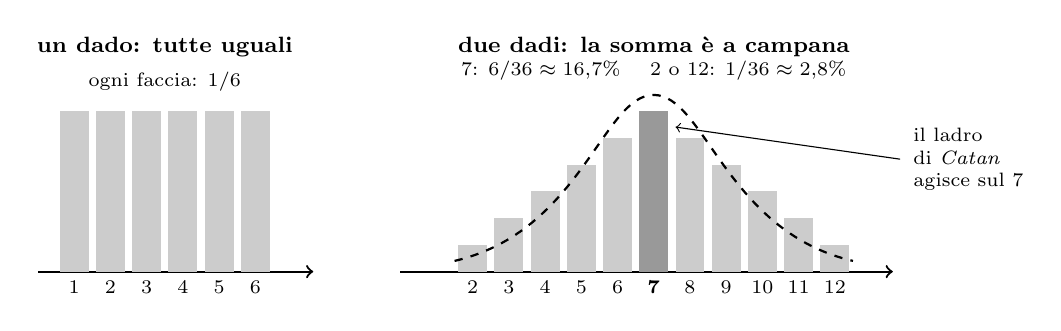
\begin{tikzpicture}[font=\small, x=0.46cm, y=0.34cm]
  % un dado
  \node[font=\footnotesize\bfseries] at (3.5,8.4) {un dado: tutte uguali};
  \draw[thick, ->] (0,0) -- (7.6,0);
  \foreach \v in {1,...,6} {
    \fill[gray!40] (\v-0.4,0) rectangle (\v+0.4,6);
    \node[below, font=\scriptsize] at (\v,0) {\v};
  }
  \node[font=\scriptsize] at (3.5,7.1) {ogni faccia: $1/6$};
  % due dadi
  \begin{scope}[shift={(10,0)}]
    \node[font=\footnotesize\bfseries] at (7,8.4) {due dadi: la somma è a campana};
    \draw[thick, ->] (0,0) -- (13.6,0);
    \foreach \v/\h in {2/1,3/2,4/3,5/4,6/5,8/5,9/4,10/3,11/2,12/1} {
      \fill[gray!40] (\v-0.4,0) rectangle (\v+0.4,\h);
      \node[below, font=\scriptsize] at (\v,0) {\v};
    }
    \fill[gray!80] (6.6,0) rectangle (7.4,6);
    \node[below, font=\scriptsize\bfseries] at (7,0) {7};
    \draw[thick, dashed] (1.5,0.4) .. controls (5,1.5) and (5.6,6.6) .. (7,6.6)
                          .. controls (8.4,6.6) and (9,1.5) .. (12.5,0.4);
    \node[font=\scriptsize, align=center] at (7,7.5) {7: $6/36 \approx 16{,}7\%$ \quad
      2 o 12: $1/36 \approx 2{,}8\%$};
    \node[font=\scriptsize, align=left, anchor=west] at (13.9,4.2) {il ladro\\di
      \emph{Catan}\\agisce sul 7};
    \draw[->, thin] (13.8,4.2) -- (7.6,5.4);
  \end{scope}
\end{tikzpicture}
\caption{Il principio del random controllato: un dado è uniforme, ma la somma di due dadi
non lo è. Il risultato più probabile, il 7, è quello su cui \emph{I Coloni di Catan} mette
il ladro che punisce chi accumula troppe risorse. La linea tratteggiata richiama la curva a
campana che si ottiene sommando molti elementi casuali (la macchina di Galton del video).}
\label{a15:fig:campana}
\end{figure}

\paragraph{Approfondimento: calcolare o simulare.} Schell, in \emph{The Art of Game Design},
usa proprio \emph{Monopoly} come esempio del \emph{metodo Monte Carlo}: quali caselle sono
visitate più spesso? ``Sarebbe quasi impossibile ricavarlo in teoria'', ma una semplice
simulazione che lancia i dadi e muove le pedine qualche milione di volte risponde in pochi
minuti. È il terzo modo di calcolare una probabilità, accanto ai due di Diego: quando il
sistema è troppo intrecciato per l'albero o per la moltiplicazione, si prova, molte volte,
e si contano i risultati. Lo stesso Schell ricorda (è una delle sue ``regole'' della
probabilità) che una cosa è la probabilità reale e un'altra quella \textbf{percepita} dai
giocatori: chi ha provato tre volte un attacco senza mai colpire tende a concludere che
``non colpisce mai''. Per chi progetta, conta anche la seconda.

% ---------------------------------------------------------------------
\section{Le nove combinazioni: input, output, combinato}
\label{a15:sec:nove}

``Ora, il random nei videogiochi e nei giochi da tavolo si usa in tre modi: come
\textbf{input}, come \textbf{output} o \textbf{combinato}.'' È la prima cosa da capire. E
ciascuno dei tre momenti può usare ciascuno dei tre tipi di random visti prima: un input
può essere random vero, pseudo-random o random controllato, e lo stesso vale per l'output.
Ne vengono \textbf{nove combinazioni} possibili (tabella~\ref{a15:tab:nove}).

La differenza tra i tre momenti sta tutta \textbf{nella posizione della casualità rispetto
alla decisione del giocatore} (figura~\ref{a15:fig:momento}): prima della decisione
(l'input: il caso stabilisce \emph{con che cosa} si gioca), dopo la decisione (l'output:
il caso stabilisce \emph{come va} ciò che si è deciso), o entrambe nella stessa decisione
(il combinato).

\begin{figure}[htbp]
\centering
\begin{tikzpicture}[
  font=\small,
  a15box/.style={draw, thick, rounded corners=3pt, minimum height=0.9cm, text width=2.4cm,
                 align=center},
  a15rnd/.style={draw, thick, dashed, rounded corners=3pt, minimum height=0.9cm,
                 text width=2.4cm, align=center, fill=gray!15},
  a15arr/.style={-{Stealth[length=2.6mm]}, thick}
]
  % input
  \node[font=\footnotesize\bfseries, anchor=east] at (-0.3,0) {input};
  \node[a15rnd] (i1) at (1.4,0) {caso\\{\footnotesize carte, setup}};
  \node[a15box] (i2) at (4.8,0) {\textbf{decisione}};
  \node[a15box] (i3) at (8.2,0) {risultato\\{\footnotesize certo}};
  \draw[a15arr] (i1) -- (i2); \draw[a15arr] (i2) -- (i3);
  % output
  \node[font=\footnotesize\bfseries, anchor=east] at (-0.3,-1.6) {output};
  \node[a15box] (o1) at (1.4,-1.6) {situazione\\{\footnotesize nota}};
  \node[a15box] (o2) at (4.8,-1.6) {\textbf{decisione}};
  \node[a15rnd] (o3) at (8.2,-1.6) {caso\\{\footnotesize successo, entità}};
  \draw[a15arr] (o1) -- (o2); \draw[a15arr] (o2) -- (o3);
  % combinato
  \node[font=\footnotesize\bfseries, anchor=east] at (-0.3,-3.2) {combinato};
  \node[a15rnd] (c1) at (1.4,-3.2) {caso\\{\footnotesize la carta pescata}};
  \node[a15box] (c2) at (4.8,-3.2) {\textbf{decisione}};
  \node[a15rnd] (c3) at (8.2,-3.2) {caso\\{\footnotesize il danno da 0 a $n$}};
  \draw[a15arr] (c1) -- (c2); \draw[a15arr] (c2) -- (c3);
  \node[font=\footnotesize, text width=11cm, align=center] at (4.2,-4.5) {grigio
    tratteggiato: dove entra la casualità. Nel combinato i due momenti stanno
    \emph{nella stessa decisione}, non in fasi diverse del gioco};
\end{tikzpicture}
\caption{I tre momenti della casualità rispetto alla decisione del giocatore. L'input
``inietta'' il caso prima che il giocatore scelga; l'output lo mette dopo, sul successo o
sull'entità del risultato; il combinato fa entrambe le cose nella stessa decisione.}
\label{a15:fig:momento}
\end{figure}

\begin{table}[htbp]
\centering
\small
\begin{tabular}{@{}>{\raggedright\arraybackslash}p{2.3cm}>{\raggedright\arraybackslash}p{3.7cm}>{\raggedright\arraybackslash}p{3.7cm}>{\raggedright\arraybackslash}p{3.7cm}@{}}
\toprule
 & \textbf{Random vero} & \textbf{Pseudo-random} & \textbf{Random controllato} \\
\midrule
\textbf{Input} & pescare da un mazzo appena mischiato (poker a cinque carte) & pescare
  sapendo che cosa è già uscito (Texas Hold'em, stoppa, briscola contata) & mazzi costruiti
  per pescare ciò che serve (i mazzi \emph{combo} di \emph{Magic}) \\
\addlinespace
\textbf{Output} & il D20 della palla di fuoco & l'esito tirato da un'app o da un computer &
  il dado con modificatore $+2$ (``sotto il 3 non vai'') \\
\addlinespace
\textbf{Combinato} & pesco una carta e il suo danno è random & la stessa cosa gestita da
  un'app & \emph{push your luck}, scelte tra tre, dadi forgiati \\
\bottomrule
\end{tabular}
\caption{Le nove combinazioni tra i tre tipi di random e i tre momenti della decisione,
con un esempio per casella tratto dalla lezione (alcune caselle sono ricostruite dagli
esempi successivi: Diego elenca le combinazioni, ma non le illustra una per una).}
\label{a15:tab:nove}
\end{table}

% ---------------------------------------------------------------------
\section{L'input random}
\label{a15:sec:input}

\subsection{Che cos'è: il caso prima della decisione}

La definizione sulla slide: l'input random è ``\emph{the injection of chance before the
player makes a decision}''; fornisce condizioni incerte, o risorse, con cui il giocatore
deve poi lavorare strategicamente. È \textbf{l'aggiunta di un elemento casuale, o
statisticamente basato, che crea incertezza nelle condizioni o nello stato del gioco}, e con
cui i giocatori devono poi gestire il resto della partita.

``Sembra complesso, ma il modo più facile è \textbf{pescare le carte}.'' Molti giochi dicono
``all'inizio del turno pesca una carta'': quella carta è randomica, o pseudo-randomica.

\paragraph{Poker a cinque carte e Texas Hold'em.} Nel poker ``all'italiana'', quello a
cinque carte\footnote{Diego cerca il nome (``non briscola\ldots{} poker''): ``di tanto mi
vengono i giochi italiani''.}, non si ha idea di che cosa si peschi: si pescano le carte, si
guardano, si decide. È input \textbf{random}. Nel \textbf{Texas Hold'em} la mano è invece
\textbf{pseudo-random}: dalle carte scoperte sul tavolo si ricavano informazioni sul resto
del mazzo.

\paragraph{Contare le carte.} Diego chiede che cosa voglia dire \textbf{contare le carte} a
poker, e Jacopo, ``rivela i segreti'', risponde: pur non essendo un giocatore di poker, si
conta la quantità di carte rimaste e si calcola la probabilità che esca quella che serve,
per esempio il quarto asso. ``Esatto'': se i quattro assi sono già sul tavolo, la
probabilità che un altro giocatore abbia un asso è zero. È semplice, ma è importante,
perché trasforma il caso in informazione.

\subsection{La stoppa: un input che diminuisce nel tempo}

C'è ``un gioco italiano che io cito sempre'', perché è interessantissimo proprio su questo:
la \textbf{stoppa}. È un gioco di carte del Sud Italia, di cui non si sa bene chi l'abbia
inventato: un ``poker italiano'' con una caratteristica particolare. Si gioca \textbf{a
fasi}. Nella prima fase ogni giocatore riceve \textbf{tre carte}, che hanno punteggi come nel
poker: si può avere una mano buona o cattiva.

\paragraph{Una mano.} Diego, Jacopo e Davide giocano. Diego ha una buona mano e rilancia;
Davide ha una buona mano e vede; Jacopo ha una brutta mano e ``si fa i fatti suoi''. Diego e
Davide continuano a rilanciare, senza pescare altre carte, finché nessuno rilancia più e si
rivelano le carte. Diego ha un \textbf{tris di 7}, un buon punteggio\footnote{Nella
trascrizione ``il 7 vale 21 punti nella stoppa, quindi 7, 21, 42, 63'': i valori sono
riportati come detti, ma la sequenza è confusa e non permette di ricostruire con certezza il
sistema di punteggio.}; Davide rivela di aver bluffato, e Diego vince.

\paragraph{Le carte restano.} Nel poker a questo punto si rimischia, fine. Nella stoppa,
invece, \textbf{tutti i giocatori tengono le proprie carte}, Jacopo compreso, e le mettono
da parte. Diego ha vinto la mano, ma ora tutti sanno che quei tre 7 non sono più nel mazzo e
che li ha lui; e Diego sa che cosa aveva Davide, ma non che cosa aveva Jacopo. Si continua
così finché il mazzo finisce e ciascuno ha \textbf{dieci carte}: a quel punto si devono
scegliere tre carte tra le proprie dieci per fare la mano migliore.

\paragraph{Vincere vuol dire rivelarsi.} Che cosa significa? Che \textbf{più si è vinto nelle
mani precedenti, più si è rivelata la propria mano finale}: se si è vinto tanto, tutti hanno
visto le carte, e sanno esattamente che cosa c'è fra quelle dieci. Chi ha perso, o ha
nascosto sempre le carte (come Jacopo), resta un mistero. È \textbf{un esempio di input
random che diminuisce nel tempo}: si parte da un input del tutto casuale, l'intero mazzo, e
pian piano l'informazione cresce e il caso si riduce.

\subsection{\emph{Magic}: trasformare il random in pseudo-random}

Diego chiede chi gioca a \textbf{\emph{Magic: The Gathering}}, \emph{Yu-Gi-Oh!} o altri
collezionabili; Jacopo gioca a \emph{Magic}. Una delle caratteristiche di \emph{Magic} è
proprio \textbf{partire dal mazzo randomico e trasformarlo in pseudo-randomico}, con carte che
permettono di \textbf{controllare la pescata}. Jacopo fa un esempio: ci sono carte che
fanno guardare le prime tre del mazzo, o rimischiare il mazzo; ``hai tanto controllo''.
``Esattamente.'' I cosiddetti \textbf{mazzi \emph{combo}}, che vincono se ottengono una certa
combinazione di carte, non sperano di pescare per caso la carta giusta: inseriscono tutta
un'altra serie di carte che trasformano il mazzo in pseudo-randomico e \textbf{aumentano
statisticamente la probabilità} di ottenere ciò che serve.

\paragraph{Investire risorse per controllare il caso.} L'input random, quindi, è qualcosa
che avviene \textbf{prima} delle decisioni e che i giocatori usano \textbf{per} decidere; e
molti giochi lo collegano alla possibilità di \textbf{controllare quella randomicità a
proprio vantaggio}, di solito \textbf{investendo risorse}. Un gioco inventato: ogni turno si
pesca una carta e si fa ciò che dice. Diego pesca ``3 risorse'' e passa; Oksana pesca ``5
risorse''; Diego (lo studente) pesca ``5 risorse''. Poi Diego può scegliere: pescare, o
investire le risorse in un'abilità speciale che dal turno successivo gli fa \textbf{vedere
due carte e sceglierne una}. È una forma tipica di \textbf{progressione} nei giochi da
tavolo: si inizia con un input completamente casuale (random vero) e lo si trasforma in
\textbf{random controllato}, diventando più forti. Guadagnando abilità, sbloccando risorse,
si ottiene \textbf{più controllo}.

\subsection{\emph{Monopoly}: dal random al random controllato}

``Chi riesce a dirmi dove sta la trasformazione da random a controllato in
\emph{Monopoly}?'' Silenzio (``non abbiamo la bellissima botta di Monopoly'', scherza
qualcuno). Diego aiuta: come si guadagnano soldi a \emph{Monopoly}? Gli studenti rispondono:
quando qualcuno finisce sulle tue proprietà; quando passi dal via (200); quando peschi la
carta giusta negli imprevisti. Il via non si controlla, e lo si esclude; gli imprevisti
nemmeno. Resta un elemento, e uno studente lo trova: \textbf{gli scambi}, dove ``c'è del
controllo'', perché si decide, si contratta sul valore effettivo, sui soldi, sulle ipoteche.
``Bravo! Si gioca su quello.''

\paragraph{Il gioco in una frase.} Non si può sapere dove finirà un avversario, ma \textbf{se
si possiede il 70\% delle proprietà, ci finirà}. ``E questo è il gioco del
\emph{Monopoly}'': trasformare il random vero in random controllato, \textbf{solo in versione
input}. Per questo, secondo Diego, \emph{Monopoly} è un gioco ``battuto'': esiste una
strategia ottimale, la si può cercare (``\emph{Monopoly how to play perfectly}'') e diventare
campioni\footnote{È un'espressione forte: \emph{Monopoly} non è un gioco ``risolto'' nel
senso matematico in cui lo sono, per esempio, la dama o il tris, anche perché contiene una
forte componente di trattativa. Esistono però analisi molto approfondite (con le catene di
Markov) su quali proprietà rendono di più e quando conviene costruire, ed è a queste che
Diego si riferisce.}. Uno dei principi è comprare le caselle che stanno ``intorno al 7''
rispetto ai punti di passaggio più frequenti, perché statisticamente ci si finisce sopra.
``Può sembrare banale, riduttivo'', ma è uno dei giochi di maggior successo della storia, e
si basa soltanto sul dare ai giocatori la possibilità, con la loro competenza, di
trasformare l'input random in random controllato.

\subsection{Ruoli nascosti e \emph{setup} variabili}

Chi conosce \textbf{\emph{Secret Hitler}}, \textbf{\emph{The Resistance}} o \textbf{\emph{Lupus
in fabula}} (\emph{Werewolf})? Jacopo conosce \emph{Secret Hitler}; Davide conosce meglio
\emph{Werewolf}: c'è un gruppo che deve eliminare gli altri, e quelli che si conoscono tra
loro sono in svantaggio numerico. ``Esattamente.'' Qui il punto di partenza è che
\textbf{il ruolo è casuale}: si può essere nazista o della resistenza in \emph{Secret
Hitler}, lupo mannaro o umano in \emph{Werewolf}; ma poi si deve giocare, e l'abilità di
giocare dipende dal ruolo avuto. Lo stesso vale per il videogioco \textbf{\emph{Among
Us}}\footnote{Nella trascrizione ``da Mongas''.}, con gli infiltrati e gli altri: il gioco si
basa tutto sull'individuare chi è l'altro \textbf{partendo dall'input random}.

\paragraph{Gli scenari.} Infine, i \textbf{\emph{variable setup}}: chi gioca a D\&D o ad altri
giochi di ruolo da tavolo sa che gli scenari sono letteralmente un input random: si parte da
uno scenario che dà delle possibilità. L'input random è quindi \textbf{la capacità del
designer di creare una situazione più o meno controllata}, usando le tecniche viste (il
random controllato in particolare), per dare \textbf{scelte interessanti} ai giocatori.

\subsection{La briscola: il rischio di contare troppo}

Un altro esempio, la \textbf{briscola}, che ``penso conosciate tutti''. La primissima cosa che
avviene è \textbf{rivelare la briscola}: e la propria mano può passare ``da una schifezza a
meravigliosa'' in base al seme, ma anche in base alla carta stessa che è stata rivelata. Sapere
che l'ultima carta è l'asso di briscola, o il tre, o il due (gli estremi, le carte che valgono
tanto e quelle che ``non valgono una ceppa'') cambia completamente la partita.

\paragraph{Il ``mago'' delle superiori.} Chi ha giocato alle superiori, quando la briscola
``era lo standard'', ricorderà che c'è sempre qualcuno che all'ultimo giro dice: ``tu avrai
un carico; tu hai sicuramente due carte di briscola, probabilmente il 7''. È un mago? ``Un Da
Vinci incompreso? No.'' \textbf{Ha contato le carte}, in base a come si è giocato. Sta
\textbf{comprendendo l'input random e togliendolo}, controllandolo. Se si sanno tutte le carte
che tutti hanno in mano, si può giocare la partita perfetta; e infatti a quel punto quella
persona dice: ``tagliamo corto: tu vincerai la seconda mano, io la prima, voi la terza''. Ed è
così, perché giocare diversamente sarebbe giocare male.

\paragraph{Il rischio.} Ecco il rischio dell'input random: \textbf{se si dà al giocatore
troppo controllo sull'input, il random sparisce}, perché il gioco diventa prevedibile. E una
cosa prevedibile è come il finale della briscola: ``è inutile che giochiamo le ultime tre
mani''.

\subsection{I vantaggi dell'input random}

Diego passa ai pro e ai contro, con le definizioni in inglese sulle slide (``i cosi ve li
lascio lì'').

\paragraph{\emph{Meaningful decision making}.} ``\emph{Players interpret random setup and make
optimal choices with constraints}''; sulla slide c'è anche l'esempio di \textbf{\emph{7
Wonders}}, con il \emph{draft} delle carte e le scelte tra opzioni casuali. Se il punto di
partenza è casuale, i giocatori devono fare \textbf{scelte complesse}, perché non possono
avere la partenza ottimale né sapere come andranno le cose. Questo aggiunge valore
\textbf{tattico}, non strategico, e Diego insiste sulla differenza:
\begin{itemize}
  \item \textbf{strategico} vuol dire \textbf{nel lungo periodo}: una strategia di guerra è
        ``l'anno 1 invaderemo e raccoglieremo risorse, l'anno 2 faremo questo'';
  \item \textbf{tattico} è \textbf{la battaglia}: ``ci stiamo sparando addosso'', si decide
        minuto per minuto.
\end{itemize}
Le scelte di input random sono \textbf{tattiche}: si pescano le carte e si ha qualche minuto
per decidere, non tre ore. Nei giochi di carte, \textbf{il mazzo è una scelta strategica}
(lo si è costruito con il \emph{deck building}); \textbf{la mano che capita è tattica}: può
essere perfetta o, ``sfiga vuole'', terrificante.

\paragraph{\emph{Replayability}: \emph{Cosmic Encounter}.} Una partenza casuale
\textbf{aumenta la rigiocabilità}, perché ogni tanto capita la mano fortunata, o quella
strana. L'esempio è \textbf{\emph{Cosmic Encounter}}, che nessuno conosce (``la maggior parte
della gente dice di no''): ``se siete interessati al random, è il gioco che dovreste studiare
più di tutti''. Le regole di base sono semplicissime: ogni giocatore ha \textbf{5 pianeti}, e
su ogni pianeta ci sono navi spaziali. Diego (rosso) attacca Jacopo (verde) per conquistargli
un pianeta, con 10 navi; Jacopo ne ha 5 sul pianeta. Jacopo gioca una carta $+10$, e arriva a
15; Diego gioca una carta $+5$, e arriva a 25 (il conto a voce è un po' confuso, ma il senso è
chiaro): vince Diego, che conquista il pianeta. ``Che gioco schifoso'', direte; ``che palle!''
Questa è solo la base.

\paragraph{Gli alieni.} La cosa grande di \emph{Cosmic Encounter} è che \textbf{ognuno ha un
alieno}, e ogni alieno ha \textbf{un'abilità che cambia completamente la partita}. Con tutte
le espansioni, dice Diego, ce ne sono ``qualcosa come 900''; ogni partita è una combinazione
di cinque alieni, e le possibilità sono enormi\footnote{Diego dice ``900 alieni'' e poi ``5
elevato alla 900''. Il numero di alieni, anche con tutte le espansioni, è dell'ordine di
qualche centinaio; e il conto corretto per scegliere 5 alieni fra $n$ è il coefficiente
binomiale $\binom{n}{5}$, non $5^{n}$. Anche così il numero resta enorme: con 200 alieni le
combinazioni di cinque sono circa 2,5 miliardi.}. Due esempi da partite vere.
\begin{itemize}
  \item Una partita tra Diego, il suo migliore amico e la moglie di lui. Diego ha un alieno che,
        scartando una carta, ne recupera una dal proprio cimitero; la moglie dell'amico può
        \textbf{nominare una carta} nella mano avversaria e, se c'è, rubarla; l'amico può far
        scartare a tutti la mano e far ripescare sette carte a caso. I poteri si
        contrastavano a vicenda: se Diego usava la sua abilità, gli altri vedevano quale carta
        recuperava; la moglie dell'amico allora la nominava (``secondo me hai questa carta in
        mano?''); e se l'amico vedeva che la moglie aveva preso una carta forte, faceva
        scartare tutto. ``Questa combinazione non era mai successa.''
  \item Un alieno che la trascrizione chiama \textbf{``Ace''}, ``il campione''\footnote{Il nome
        dell'alieno non è verificabile; il capitolo lo riporta come detto.}, per vincere deve
        conquistare \textbf{un solo pianeta} invece di cinque. Facilissimo? No: diventa
        \textbf{il nemico pubblico numero uno}, perché tutti sanno che se conquista anche solo
        un pianeta vince la partita. Il gioco si trasforma da tutti contro tutti in
        \textbf{quattro contro uno}, e chi ha quell'alieno deve giocare in modo super difensivo
        e aspettare il momento giusto.
\end{itemize}
In base agli alieni pescati, la partita cambia completamente: l'input random crea
``infinita'' rigiocabilità.

\paragraph{\emph{Encouraging skill}: livellare le abilità.} ``Questo è estremamente
importante'': un input random \textbf{può livellare la differenza di abilità} tra i
giocatori. Se un giocatore mediocre gioca contro un campione, e il campione ha avuto una mano
sfortunata o il mediocre una mano fortunata, la differenza si assottiglia.

\paragraph{L'esercizio del torneo di poker.} Diego propone un esperimento mentale. Non avete
mai giocato a poker, in nessuna versione; siete finiti, in qualche modo, nella finale del
torneo più importante del mondo, contro i tre campioni del mondo, e in palio ci sono 10
milioni di euro. \textbf{Quale strategia applicare per ridurre la differenza di abilità}?
``Pensateci.'' Uno studente propone di contare le carte; ma i campioni sanno contare meglio.
Allora: che cosa rende bravo un giocatore professionista? Contare le carte, e soprattutto
\textbf{prevedere che cosa faranno gli altri}, leggerne il comportamento; la \emph{poker
face}, la capacità di non mostrare emozioni. Imitare il loro comportamento? Sanno farlo
meglio. Davide ride: ha capito. La risposta è \textbf{non guardare le proprie carte}. ``Non
puoi intuire come io gioco, se nemmeno io so come sto giocando.'' Tutta l'abilità degli
avversari nel prevedere le mosse si annulla, e la partita si riduce alla \textbf{fortuna}: se
le carte sono buone si vince, altrimenti si perde.

\paragraph{La fortuna del principiante.} È quella che si chiama, appunto, \textbf{fortuna del
principiante}: spesso qualcuno ha perso perché cercava di applicare tecniche avanzate contro
qualcuno che non sapeva che cosa stesse facendo, ed è rimasto fregato. Se lo si fa davvero
in un torneo, le probabilità aumentano, ``ma tutti vi odieranno tantissimo'': è una strategia
conosciuta e i professionisti la detestano, perché vogliono giocare con la \emph{poker face}.
``Però non è tecnicamente illegale.''

\subsection{I rischi dell'input random}

``Non è tutto oro quel che luccica'': ci sono dei pericoli.

\paragraph{La \emph{turn one win}.} Se le possibilità di partenza sono troppo varie, è
possibile vincere \textbf{al primo turno} per pura fortuna. Un esempio ``che fa veramente
ridere'': la madre di Diego partecipa a un torneo di \textbf{scala 40}, arriva in finale,
l'avversaria mischia, lei taglia, pesca le carte e ha la \textbf{chiusura in mano}: tredici
carte perfette, vince il torneo. ``Non ci puoi fare niente.'' Nella scala 40 non è un
problema, perché succede raramente; ma la domanda da porsi, con l'input random, è
\textbf{quanto è possibile essere del tutto sfortunati o del tutto fortunati}.

\paragraph{Il solitario di Diego.} Da studente, Diego aveva provato a fare un
\textbf{solitario}: si disponevano delle carte sul tavolo e si cercava di fare una serie di
cose. Il problema: \textbf{se la carta negativa non finiva in uno dei quattro angoli, il
solitario era impossibile da risolvere}. Era una condizione di partenza troppo sbilanciata
(una \emph{uneven condition} troppo aggressiva): non è giusto perdere per questo. La
soluzione fu togliere la carta ``sfigata'' dal mazzo da mischiare e farla \textbf{aggiungere
dal giocatore in uno dei quattro angoli, a sua scelta}, rimuovendo un'altra carta. Così la
condizione si verificava sempre, e il solitario funzionava.

\paragraph{La morale.} Si possono inserire elementi che \textbf{controllano l'input random e
lo depotenziano} quando è ``troppo rotto'': lo riducono di potenza, lo rendono meno efficace,
oppure lo giustificano. In \emph{Arkham}, se nella mano iniziale c'è una
\textbf{debolezza}, la si toglie, la si rimischia nel mazzo e si pesca un'altra carta:
perché iniziare la partita con una debolezza in mano ``è finita''. La mischiata è casuale,
``ma se è proprio sfiga, non va bene''. Anche \emph{Magic} ha qualcosa del genere, il
\textbf{\emph{mulligan}}, su cui la lezione tornerà.

\paragraph{La paralisi da analisi.} Succede soprattutto con giochi nuovi o giocatori nuovi:
se l'input random è troppo forte (cinque carte in mano, più cinque pedine casuali, più cinque
altre cose casuali: venti elementi casuali), è \textbf{troppa roba da calcolare per la
tattica}. ``Ricordatevi: strategia contro tattica.'' Se si hanno cinque minuti per decidere e
venti cose casuali da valutare, non ce la si fa. In questi casi alcuni elementi devono
essere \textbf{non casuali}: per esempio il numero di risorse; o il mazzo costruito dal
giocatore, così che la pescata è casuale ma il contenuto del mazzo è noto; o
\textbf{l'obiettivo}. Ci sono giochi in cui anche l'obiettivo è casuale, e non si sa che cosa
fare finché non lo si è pescato.

\paragraph{La riduzione della strategia, o una falsa strategia.} Se \textbf{tutto} è casuale,
il gioco è rigiocabile ma non profondo: è ``una serie di condizioni casuali''. Come lo si
limita? Con \textbf{obiettivi non casuali}. Se la partenza è casuale ma l'obiettivo no, si
può sempre costruire una strategia verso l'obiettivo; se sono casuali entrambi, forse no.

\paragraph{Il controllo limitato.} Infine il \textbf{\emph{limited player control}}: se tutto
è casuale, il giocatore non ha scelta. L'input random dovrebbe stare \textbf{all'inizio}, e
poi la decisione deve essere del giocatore.

Nessun dubbio. Diego propone la pausa, ma gli studenti preferiscono continuare: ``facciamo
l'output e poi dopo facciamo la pausa''.

\subsection{Le linee guida}

Prima di passare all'output, Diego riassume l'input random con qualche indicazione pratica
(tabella~\ref{a15:tab:input}).

\paragraph{Dove guardare.} Il \emph{deck building}, i giochi
``\emph{layer}''\footnote{Così nella trascrizione: potrebbe essere ``\emph{legacy}'',
``\emph{player}'' o altro; non è ricostruibile.}, i \textbf{giochi asimmetrici} e il
\textbf{\emph{drafting}} sono tutti esempi di ottimi input random da prendere come
riferimento; la slide ne elenca sette, ``come sette caratteristiche''.

\paragraph{La regola unica.} Se si vuole ridurre tutto a una sola regola: \textbf{l'input
random deve far sentire il giocatore più potente}, offrendogli \textbf{più scelte} di quelle
che avrebbe senza, \textbf{ma non deve togliergli l'\emph{agency}}. Il giocatore non deve
sentire di non avere controllo su ciò che avviene: non che il risultato sia necessariamente
``corretto'', ma che \textbf{si senta} in controllo. Ed è qui che entra il random controllato:
\textbf{i giochi basati sull'input random nascono input e finiscono controllati}.

\paragraph{Le cento partite.} Un suggerimento personale: quando si fa un gioco con input
random, \textbf{si giochino cento partite}. Se nel \textbf{30\% delle vittorie o più} conta la
fortuna, il gioco è troppo basato sulla fortuna; \textbf{la fortuna dovrebbe influire sul
20\% delle vittorie}\footnote{Diego non dice come stabilire, in pratica, se una vittoria
``è dovuta alla fortuna''. Un modo possibile è far giocare insieme persone di abilità nota e
contare quante volte vince chi è meno esperto, o confrontare i risultati con quelli di una
strategia casuale; ma è un'aggiunta del capitolo.}.

\paragraph{L'interessante prima del giusto.} E un altro consiglio ``da persona che fa questa
roba da tanti anni'': \textbf{con il random, favorite l'interessante invece del giusto}. Dire
``questo random è bilanciato'' è meno funzionale, in \emph{game design}, che dire ``questo
random è interessante''. Se poi si scopre che è troppo sbilanciato, \textbf{si aggiunge una
regola per bilanciarlo}, come la debolezza di \emph{Arkham} o il \emph{mulligan}. Pescare
carte a caso è interessante; e ``interessante vince sempre rispetto a giusto''.

\begin{table}[htbp]
\centering
\small
\begin{tabular}{@{}>{\raggedright\arraybackslash}p{3.4cm}>{\raggedright\arraybackslash}p{5.0cm}>{\raggedright\arraybackslash}p{5.2cm}@{}}
\toprule
\textbf{Aspetto} & \textbf{Che cosa succede} & \textbf{Esempi e rimedi} \\
\midrule
\multicolumn{3}{@{}l}{\emph{Vantaggi}} \\
Decisioni sensate & la partenza imperfetta chiede scelte \textbf{tattiche} & la mano
  (tattica) contro il mazzo (strategico); \emph{7 Wonders} \\
\addlinespace
Rigiocabilità & ogni partenza è diversa & gli alieni di \emph{Cosmic Encounter} \\
\addlinespace
Livellare le abilità & la mano fortunata avvicina principiante e campione & il poker
  giocato senza guardare le carte \\
\midrule
\multicolumn{3}{@{}l}{\emph{Rischi}} \\
\emph{Turn one win} & si vince (o si perde) per la sola partenza & la chiusura in mano a
  scala 40; il solitario di Diego: la carta ``sfigata'' piazzata dal giocatore; le
  debolezze di \emph{Arkham}; il \emph{mulligan} \\
\addlinespace
Paralisi da analisi & troppi elementi casuali da valutare & rendere fissi risorse,
  contenuto del mazzo, obiettivo \\
\addlinespace
Falsa strategia & tutto casuale: rigiocabile ma non profondo & obiettivi non casuali \\
\addlinespace
Poco controllo & il giocatore non sceglie & il caso all'inizio, poi la decisione \\
\addlinespace
Troppo controllo & il random sparisce, tutto è prevedibile & il finale della briscola \\
\bottomrule
\end{tabular}
\caption{L'input random in sintesi. Regola d'oro: nasce input e finisce controllato, e deve
far sentire il giocatore più potente senza togliergli l'\emph{agency}; la fortuna dovrebbe
decidere circa il 20\% delle vittorie, non il 30\% o più.}
\label{a15:tab:input}
\end{table}

\paragraph{Approfondimento: caso e abilità secondo il pubblico.} Brathwaite e Schreiber, in
\emph{Challenges for Game Designers}, dedicano un capitolo all'equilibrio tra caso e
abilità che parte esattamente dalle due idee di Diego. La prima: \textbf{il pubblico}. I
bambini piccoli non hanno ancora gli strumenti per decisioni strategiche e giocano volentieri
a giochi di pura fortuna (``spesso sono convinti che tirare numeri alti con i dadi sia
un'abilità''); i giocatori competitivi vogliono che nessun tiro di dado rovini una giocata
perfetta; i giocatori ``sociali'' tollerano molta più fortuna; le famiglie hanno bisogno di
un po' di fortuna perché i bambini possano battere gli adulti. La seconda: \textbf{la fortuna
livella}. ``Più fortuna c'è in un gioco, più il campo è livellato'': se vince sempre il più
bravo, le uniche partite interessanti sono quelle tra pari; e un po' di caso toglie anche un
po' di amarezza alla sconfitta, perché chi vince può sentirsi più abile e chi perde può
dare la colpa ai dadi. Il libro propone anche i segnali da cercare nei \emph{playtest}: se
i giocatori si annoiano, forse c'è troppa fortuna (si converta qualche elemento casuale in
una decisione); se un giocatore stravince sugli altri, forse c'è troppa abilità (si aggiunga
un po' di casualità, o un meccanismo di recupero). E, come Diego, suggerisce di
\textbf{scambiare} caso e decisione: ``pagate 50 prima di tirare, e tirate tre dadi
scegliendone due'' è il loro esempio su \emph{Monopoly}, ed è esattamente un input random
reso controllato in cambio di risorse.

% ---------------------------------------------------------------------
\section{L'output random}
\label{a15:sec:output}

\subsection{Che cos'è: il caso dopo la decisione}

Diego apre con alcune GIF che gli piacciono (giocatori di \emph{Commander} e una giocatrice
che gioca ``un sacco di mazzi \emph{combo}''). L'output random è \textbf{esattamente
l'opposto} dell'input: il random non è sulle risorse che si hanno, ma \textbf{sul risultato
dell'azione}.

\paragraph{La palla di fuoco.} Il modo più semplice per definirlo è \textbf{D\&D}. Ho
un'abilità: lanciare una \textbf{palla di fuoco} in faccia all'avversario. Se colpisco o meno
quel giocatore, o quel PNG, dipende dai dadi: con 15 o più colpisco, con 14 o meno no; e il
danno dipende dal numero di dadi che lancio\footnote{È una semplificazione: nelle regole
della quinta edizione di D\&D, contro la palla di fuoco è il bersaglio a tirare un
\emph{tiro salvezza} su Destrezza, che dimezza il danno, e il danno è $8d6$. Il principio
che Diego illustra non cambia: la decisione è certa, l'esito è affidato ai dadi.}. Qui non è
la decisione, né l'abilità, a essere random: so di avere la palla di fuoco, ho deciso di
usarla, e ne ho il totale controllo, perché fa parte del mio personaggio (``non è che ho
pescato la carta palla di fuoco''). Ma \textbf{se colpisco e quanto danno faccio}, quello è
random.

\paragraph{La definizione.} L'output random è quando \textbf{la casualità avviene dopo che il
giocatore ha preso una decisione}. Di solito influenza \textbf{il successo o il fallimento},
oppure \textbf{la magnitudo}, cioè l'entità di quel successo o fallimento. Il giocatore prima
si \textbf{impegna} (\emph{commits}) in una decisione, un piano, una tattica; poi il caso gli
dice se ha funzionato e, nel caso, quanto. È all'estremo opposto dello spettro: l'input dice
quali azioni si potrebbero compiere in quel momento; l'output dice ``no, le azioni le hai già
tutte, ma il loro risultato non è scontato''.

\paragraph{La domanda di Jacopo: \emph{Betrayal}.} Jacopo chiede di un gioco come
\textbf{\emph{Betrayal at House on the Hill}}\footnote{Nella trascrizione ``B-Train'' e
``Betrayal''. Più avanti Diego lo chiama ``Betrayal of the House of the Hill''.}, un gioco di
piazzamento di tessere: si sceglie di muoversi e si pesca la tessera, e su alcune tessere ci
sono i simboli degli eventi, o si pesca un oggetto. È input e output insieme, o solo input?
Diego risponde che è \textbf{combinato}, e spiega il criterio. Quando peschi la tessera, è
input: il caso viene prima e non hai nemmeno deciso che cosa uscirà. Poi, visto il risultato,
prendi una decisione: e \textbf{se quella decisione può avere esiti diversi, c'è anche
l'output}. Se la tessera dice ``prenditi tre pizze'', è solo input; se dice ``lancia un dado
per sapere quante pizze'', è combinato. ``Hai fatto benissimo'': la lezione è un dialogo,
``intervenite quando volete''.

\paragraph{Altri esempi.} Il lancio dei dadi per un'azione in D\&D; il \textbf{Risiko} (Diego
dice \emph{Risk}, ``che sarebbe Risiko all'italiana''); i \textbf{segnalini del sacchetto} di
\emph{Arkham}: ``voglio menarlo''; peschi il segnalino $-3$, la tua abilità scende a 2, troppo
debole, non ci sei riuscito; oppure peschi ``danno critico'', o ``fallimento
critico''\footnote{Diego mescola qui il sacchetto del caos di \emph{Arkham} e il D20 di D\&D:
il racconto dei tre fallimenti critici, uno su venti, riguarda con ogni probabilità il D20.}.
Diego ci ha giocato ``letteralmente ieri'', e un suo amico ha tirato \textbf{tre volte di
seguito un fallimento critico}: ``ma che cacchio, sei proprio sfigato''. È output, perché la
decisione era presa, l'azione fatta, ma non è andata per niente bene. E poi il \textbf{lancio
della moneta}: ``se esce testa mangio l'hamburger, se esce croce prendo una pizza''. La
decisione è presa; il risultato dipende dall'elemento casuale.

\subsection{Perché usarlo: il dramma}

L'input random serve a creare scelte tattiche e a mitigare le differenze di abilità.
\textbf{L'output random serve ad aggiungere il dramma}, ``nel senso proprio del termine,
teatrale''. Quando non so se la mia azione avrà successo, sono teso: \textbf{non sapere crea
tensione per natura}.

\paragraph{\emph{Affari tuoi}.} L'esempio perfetto è ``il gioco dei pacchi su Rai 1''. Per
semplicità ci sono venti pacchi: dieci ``sfigati'' (un peluche da 10 euro, un sacchetto di
noccioline) e dieci ``fighi'' (da 5.000 a 300.000 euro). I concorrenti aprono i pacchi che
scelgono finché ne restano pochi (per esempio cinque, tre positivi e due negativi, o
viceversa); poi arriva un'\textbf{offerta}: ``ti do 40.000 euro e il gioco finisce adesso;
oppure rischi, e magari c'è ancora il pacco da 300.000''. Se si sapesse di avere il pacco
sfigato, si accetterebbe al volo; se si sapesse di avere quello da 300.000, si rifiuterebbe.
\textbf{Il dramma sta nel fatto che l'output è sconosciuto}: ``oddio, 40.000 sono tanti
soldi; ma se poi avessero quello da 300.000? E se beccano il calzino?''

\paragraph{\emph{Golden Balls}.} Un altro esempio, ``un capolavoro'', da YouTube:
\textbf{\emph{Golden Balls}}\footnote{Nella trascrizione ``la Golden Ball''. È il quiz
britannico \emph{Golden Balls} (ITV); l'episodio mostrato, con i concorrenti Nick e Ibrahim, è
uno dei più famosi del ``\emph{split or steal}''.}. Due concorrenti hanno collaborato per
accumulare una cifra (in quella puntata circa 13.000 sterline) e ora hanno davanti due
palline: \textbf{dividi} (\emph{split}) e \textbf{ruba} (\emph{steal}). Se entrambi scelgono
dividi, si dividono la somma; se entrambi scelgono ruba, nessuno vince niente; se uno sceglie
ruba e l'altro dividi, chi ha scelto ruba prende tutto. Diego fa sentire lo spezzone: Nick
dice a Ibrahim che sceglierà \emph{steal} al 100\%, e gli chiede di scegliere \emph{split},
promettendo di dividere i soldi con lui dopo lo spettacolo. Ibrahim incredulo: ``dopo che hai
preso \emph{steal}?'' ``Sì.'' Che fare? Fidarsi di una promessa ``nell'aria'', o scegliere
ruba per ripicca, ``e nessuno vince niente''? ``Fidati che i soldi te li do.'' Questa
\textbf{incertezza del risultato crea il dramma}. ``Andatevelo a vedere, se volete sapere come
va a finire.''

\paragraph{I tre vantaggi.} Ne vengono tre punti di forza.
\begin{enumerate}
  \item \textbf{Il dramma e l'intensità emotiva.} Una scelta non sicura spinge l'emotività,
        e ``fare giochi è essere emotivi'': vogliamo che i giocatori provino emozioni, e
        rendere incerto il risultato le spinge al massimo.
  \item \textbf{\emph{High risk, high reward}.} Non avere la certezza del risultato permette
        di dare al giocatore scelte \textbf{molto pericolose ma potenzialmente molto
        vantaggiose}. Se va male, ``chi è causa del suo mal pianga se stesso'': la scelta
        rischiosa l'hai fatta tu. ``Mi è capitato migliaia di volte: se azzecco questa cosa
        vinco; poi la sbaglio e ho perso.'' Con la certezza assoluta di riuscire, sarebbe
        stato noioso.
  \item \textbf{Ridurre la differenza di abilità}, come per l'input: se non sono sicuro di
        batterti, perché potrei avere un colpo di sfortuna, tu resti in partita.
\end{enumerate}

\subsection{Il rischio: troppa sfortuna}

Il rischio è che \textbf{troppa sfortuna dà fastidio}. È ciò che è successo all'amico di
Diego: tre fallimenti critici di fila tolgono al giocatore la sensazione di \emph{agency}
(``una volta va bene, ma tutte e tre le volte non è giusto''). Diego prova a fare il conto con
la calcolatrice: una possibilità su 20, tre volte, ``quindi una su 60'', l'1,6\%; uno
studente lo corregge, le probabilità vanno \textbf{moltiplicate}, ``ah, giusto, è molto più
basso''\footnote{Il conto corretto: $\left(\tfrac1{20}\right)^3 = \tfrac1{8000} =
0{,}0125\%$, cioè circa una volta su ottomila serie di tre tiri. È lo stesso errore che il
modo ``visivo'' della sezione~\ref{a15:sec:calcolo} aiuta a evitare: tre eventi indipendenti
si moltiplicano, non si sommano.}. ``Quindi è una cosa folle.'' Troppo risultato casuale
toglie ai giocatori la sensazione di avere effetto sul gioco: fanno la loro strategia, la loro
tattica, e poi non funziona mai perché hanno sfortuna. Per questo esistono \textbf{tecniche
di mitigazione}, che Diego mostra subito dopo.

\subsection{Quando: poco all'inizio, di più verso la fine}

Mentre l'input è presente all'inizio e poi diventa controllato, \textbf{l'output random non
dovrebbe essere presente all'inizio}. Qui la trascrizione si interrompe\footnote{Una stringa
ripetuta (``Output transcript'') copre una parte della spiegazione. Il senso è ricostruibile
da ciò che Diego dice dopo la pausa, quando disegna le due curve: ``l'output è l'opposto: ne
ho poco all'inizio e diventa medio a fine partita, per dare quel momento di dramma''
(figura~\ref{a15:fig:curve}). È andato perso anche l'inizio dell'esempio che segue.} e
riprende nel mezzo di un esempio, che mostra come inserire l'output alla fine \textbf{senza
annullare} ciò che è avvenuto prima.

\paragraph{Il sacchetto finale.} Siamo nella fase finale, e il gioco dice: per ogni 10 risorse
accumulate, metti nel sacchetto un segnalino del tuo colore (verde Diego, rosso Davide). Diego
ha 100 risorse, Davide 200: Davide mette 20 segnalini, Diego 10. Poi si estrae un segnalino, e
chi viene estratto vince. Diego ha comunque una possibilità, ma statisticamente Davide ne ha
di più (due su tre). Il caso finale \textbf{si basa su ciò che è successo prima}: Davide
probabilmente vincerà, ma Diego non ha abbandonato la partita, e se è fortunato vince.

\paragraph{La variante con i soldatini.} Oppure, se non si vuole far decidere la vittoria in
modo così diretto: i segnalini non decidono chi vince, ma \textbf{chi ottiene un potenziamento
speciale} per i propri soldatini nella battaglia finale. Diego e Davide hanno 20 soldatini a
testa; nel sacchetto Davide ha 20 segnalini, Diego 10. È più probabile che il potenziamento
vada a Davide, ma può andare anche a Diego, e questo \textbf{crea tensione}. Il principio:
\textbf{l'output si crea verso la fine, non deve annullare ciò che è venuto prima}, ma
costruire la possibilità che accada qualcosa di casuale senza rovinare il resto.

\subsection{Mitigare l'output random}

Se c'è troppo output random il gioco diventa brutto, ``perché c'è troppa sfiga''. Le
\textbf{tecniche di mitigazione} non servono a ridurre il random, ma a \textbf{dare ai
giocatori la possibilità di ridurre la sfortuna} (tabella~\ref{a15:tab:mitigazione}).

\paragraph{Il \emph{reroll}.} In D\&D esiste il segnalino di \textbf{ispirazione}: il master
premia chi gioca bene dandogli l'ispirazione, che si può consumare per \textbf{ritirare i
dadi} dopo un tiro sfortunato\footnote{Nella quinta edizione del 2014 l'ispirazione dà
\emph{vantaggio} (si tirano due D20 e si tiene il migliore) e va spesa prima del tiro; nella
revisione del 2024 l'\emph{ispirazione eroica} permette proprio di ritirare un dado. In
entrambi i casi è un premio che mitiga l'output.}. Così chi ha giocato bene è premiato
proprio quando l'output gli va male. \textbf{\emph{King of Tokyo}} ha ``letteralmente'' il
\emph{reroll}. E \textbf{\emph{Dicey Dungeons}}\footnote{Nella trascrizione ``Dicey
Dungeon''.}, un videogioco: si esplora un \emph{dungeon}, si tirano dei dadi e poi \textbf{li
si posiziona}. Il giocatore del video ha tirato 1, 2, 3, 4, 5 e 6 e può decidere dove
metterli: il 6 sul danno, o sul danno con un dado aggiuntivo, o sullo slot del ghiaccio. Come
li si posiziona cambia la partita: c'è un input random (i dadi lanciati), una parte
strategica (dove metterli) e un output (i dadi dell'avversario). Se si vuole massimizzare il
danno conviene mettere i dadi più alti sul danno; se si vuole massimizzare la difesa, il 6 sul
ghiaccio.

\paragraph{I modificatori.} Giochi che aggiungono \textbf{modificatori} al random: ``tira un
dado da 6, ma hai $+2$, quindi di sicuro sotto il 3 non vai''. Sapendolo, so che meno di 3
danni non li farò: ho un output random che sto controllando con i modificatori.

\paragraph{Le assicurazioni.} Le meccaniche di \textbf{\emph{insurance}}: il giocatore
\textbf{investe risorse} per assicurarsi che, se le cose vanno male, non vadano malissimo.
Diego e Jacopo devono lanciare un dado, e chi fa di più vince la battaglia. Diego spende 20
risorse per un'assicurazione: se gli esce 1, vale come 6, quindi il suo dado ha due facce 6.
Se gli esce 2 è comunque sfortunato, e ha anche perso le risorse dell'assicurazione. Jacopo,
magari, non lo fa, perché preferisce tenere le risorse per altro: anche l'assicurazione è una
scelta.

\paragraph{Il successo nel fallimento.} Il quarto modo, ``più difficile da fare ma più
interessante'' e presente in meno giochi, sono le meccaniche in cui \textbf{anche l'output
fallimentare è in qualche modo un successo}, o dà comunque delle possibilità. Diego e Jacopo
si contendono la \textbf{Kamčatka}\footnote{Nella trascrizione ``Kamciak'', ``canciacca'' e
``cranciacca''. È il territorio del Risiko.} (``un classico''), in un gioco simile al Risiko
in cui ciascuno tira un dado. La Kamčatka è di Jacopo; Diego fa 3, Jacopo 1: Diego la
conquista. Un gioco con il successo nel fallimento potrebbe dire:
\begin{itemize}
  \item chi perde un territorio \textbf{pesca una carta}: Jacopo ha perso la Kamčatka, ma
        guadagna una risorsa che magari lo aiuta;
  \item quando si tira un 1, \textbf{il dado viene messo da parte} e diventa un modificatore
        $+1$ per un lancio futuro.
\end{itemize}
Nel caso opposto (Diego attacca con tre pedine, fa 1 contro il 3 di Jacopo e perde le
pedine), invece della sconfitta e basta:
\begin{itemize}
  \item per ogni pedina persa, Diego guadagna una risorsa;
  \item oppure le pedine perse tornano nel suo ``generatore'' di pedine, e potrà generarne di
        più in futuro;
  \item oppure, se perde il lancio, ottiene \textbf{un'altra azione}, come un turno
        aggiuntivo per fare qualcos'altro.
\end{itemize}

\paragraph{Perché è difficile.} Premiare la sconfitta può essere \textbf{pericoloso}, perché
può creare scenari in cui il gioco \textbf{si blocca}: ``se chi vince vince e chi perde vince,
che cacchio sta vincendo? Vincono tutti'', e il rischio è lo stallo. Ma \textbf{piccoli bonus}
alle sconfitte possono ridurre la sensazione di ``ma che cacchio, sono sfigato''.

\begin{table}[htbp]
\centering
\small
\begin{tabular}{@{}>{\raggedright\arraybackslash}p{3.0cm}>{\raggedright\arraybackslash}p{5.4cm}>{\raggedright\arraybackslash}p{5.2cm}@{}}
\toprule
\textbf{Tecnica} & \textbf{Come funziona} & \textbf{Esempi della lezione} \\
\midrule
\emph{Reroll} & si può ritirare il dado, di solito pagando o consumando qualcosa &
  l'ispirazione di D\&D, \emph{King of Tokyo}; il posizionamento dei dadi di \emph{Dicey
  Dungeons} \\
\addlinespace
Modificatori & spostano l'intervallo dei risultati & $d6+2$: ``sotto il 3 non vai'' \\
\addlinespace
Assicurazione & si investono risorse perché il peggio non sia troppo brutto & pagare 20
  risorse perché l'1 valga 6 \\
\addlinespace
Successo nel fallimento & anche perdere dà qualcosa & la carta a chi perde la Kamčatka; l'1
  che diventa un $+1$ futuro; le pedine che tornano nel generatore; un'azione extra \\
\bottomrule
\end{tabular}
\caption{Le tecniche di mitigazione dell'output random. Non riducono il caso: danno al
giocatore modo di ridurre la sfortuna. Il successo nel fallimento va dosato, perché premiare
troppo la sconfitta porta allo stallo.}
\label{a15:tab:mitigazione}
\end{table}

\subsection{Dove usarlo}

Essendo legato al dramma, l'output random funziona soprattutto in tre famiglie di giochi.
\begin{itemize}
  \item \textbf{I giochi tematici}, con forti elementi di dramma: horror, guerra. Non nei
        giochi altamente \textbf{strategici}, dove ci deve essere meno dramma; nei giochi
        altamente \textbf{simulativi} ``potenzialmente non è corretto''; e i giochi altamente
        \textbf{sociali} hanno già il dramma nell'interazione tra le persone.
  \item \textbf{I giochi \emph{casual}}, che nessuno affronta in modo troppo competitivo:
        accettare la sfortuna ci sta, ``tanto siamo qua per farci due risate''. Si immagini
        invece di giocare tre ore a Risiko e perdere perché è uscito un 1: ``vi viene la
        rabbia''. In \textbf{\emph{Exploding Kittens}}\footnote{Nella trascrizione ``Spodding
        Kitten''.}, invece, ``hai pescato la bomba, vabbè'': sono venti minuti, ``e chi se ne
        frega''.
  \item \textbf{I giochi di \emph{risk management}}, basati sulla mitigazione di tipo
        assicurativo: c'è tanta sfortuna, e il gioco consiste nel costruire sistemi che la
        riducano, accumulando risorse o possibilità.
\end{itemize}

\paragraph{\emph{Betrayal at House on the Hill}.} È ``uno degli elementi horror di output
random più fighi''. Si gioca, se Diego ricorda bene, da tre a sei giocatori. Nella prima fase
si \textbf{esplora la casa}, che è input random; poi, in base alle azioni dei giocatori e ai
dadi, \textbf{uno di loro diventa il traditore}, il mostro che gli altri dovranno sconfiggere,
mentre il mostro deve completare un rituale o uccidere tutti, a seconda di quale combinazione
è uscita. A volte il traditore è nascosto, e deve attaccare gli altri in segreto. Si crea
proprio il momento di dramma: ``ah, lo sapevo che eri te, ci avrei scommesso tutto''.

\paragraph{Più limitato dell'input.} L'output, quindi, è molto più limitato dell'input:
\textbf{può essere molto più cattivo}, ed è molto più facile creare frustrazione. L'input è
più accettato perché ``ho le informazioni e prendo una decisione''.

\subsection{Le linee guida}

\paragraph{Il dramma, non ogni decisione.} \textbf{Usate l'output per il dramma, non per ogni
decisione}: alla fine del gioco, nei momenti risolutivi, nei momenti topici.

\paragraph{La domanda di Davide: il gioco dell'oca.} Davide chiede del \textbf{gioco
dell'oca}: è solo output random? ``Assolutamente sì, ed è la ragione per cui ai bambini piace
e agli adulti no.'' Il bambino tira un 6 e pensa: ``sono fortissimo, ho fatto 6''. L'adulto
sa che ha lanciato il dado e gli è capitato il 6: ``ho avuto fortuna''. Il bambino ``cade
nella cosa''; l'adulto sa che non ci poteva fare niente, letteralmente. Ed è proprio il
punto successivo.

\paragraph{Mitigazione limitata.} \textbf{Si limita l'output dando al giocatore la
possibilità di controllarlo con un sistema di mitigazione}; ma non infiniti sistemi di
mitigazione. Magari si hanno \textbf{cinque \emph{reroll} per tutta la partita}, e si decide
quando usarli. Ecco che diventa \textbf{una scelta strategica}: li uso all'inizio, quando mi
capita la sfortuna, o li tengo per la fine? E se il gioco finisce prima che li abbia usati
tutti, ho sbagliato, avrei dovuto consumarli meglio.

\paragraph{Legarlo al tema.} Quando lo si crea, si cerchi di \textbf{legarlo al momento
tematico del gioco}: oltre a collocarlo meccanicamente verso la fine, o comunque nei momenti di
alto dramma, lo si colleghi al \textbf{momento emotivo}, perché lo scopo dell'output random
è dare una forte risposta emotiva.

\paragraph{Il dado critico.} Un piccolo esempio da D\&D. Si tira un D20: l'1 è un fallimento
critico, il 20 un successo critico. Una regola che Diego dà ai suoi giocatori\footnote{Diego
dice che è ``presente nel manuale originale, in realtà dalla 3'', cioè dalla terza edizione;
la fonte non è verificabile, e il capitolo la tratta come una regola della casa di Diego.} è
il \textbf{dado critico}: ognuno ne ha uno, e può usarlo \textbf{al posto} di un normale D20.
Il dado critico ha effetti potenziati: \textbf{se fallisci, fallisci molto peggio; se hai
successo, hai successo molto meglio}. E lo decidi da solo. Magari lo usi quando sai di avere
molti modificatori positivi; ma ``se poi viene l'uno, su chi?'' Magari lo usi per battere il
boss finale con un colpo solo, o per convincere quel personaggio; o lo usi e fallisci, e ``ti
sei tirato la zappa sui piedi'': hai voluto il dado critico, adesso ne hai le conseguenze.
\textbf{Associare il dramma alla scelta del giocatore} è un modo semplice per togliere la
frustrazione, perché è stato il giocatore a scegliere.

\paragraph{L'esempio negativo: \emph{Killer Bunnies}.} Come riferimento in negativo,
\textbf{\emph{Killer Bunnies}}, che \textbf{mette nel finale solo l'output random} e
distrugge l'esperienza della partita\footnote{In \emph{Killer Bunnies and the Quest for the
Magic Carrot} vince chi possiede la carota magica rivelata alla fine, estratta a caso tra
quelle in gioco: chi ha più carote ha più probabilità, ma tutta la partita si decide con
un'estrazione. In apparenza somiglia al sacchetto proporzionale descritto sopra; la differenza, nella
lettura di Diego, è che il caso finale schiaccia ciò che è avvenuto prima invece di
derivarne.},
invece di fare ciò che si è detto: \textbf{basare l'output random su ciò che i giocatori hanno
fatto durante la partita}. ``Non conosco \emph{Killer Bunnies}'', direte; ma si trova
facilmente com'è il finale, e lo si capisce.

\paragraph{Approfondimento: valore atteso e rimpianto.} Schell, nel capitolo sul caso, dà
gli strumenti per ragionare sugli esempi di Diego. Il primo è il \textbf{valore atteso}:
la media dei risultati possibili pesata sulla loro probabilità. Un attacco che fa sempre 4
danni e uno che colpisce l'80\% delle volte facendone 5 hanno lo stesso valore atteso, 4;
ma il valore atteso va calcolato sul valore \emph{reale}: un fulmine che fa 40 danni il 20\%
delle volte vale 8, ma contro un nemico con 15 punti vita ne vale solo 3. Il secondo è che
\textbf{le persone non scelgono in base al valore atteso}: nell'esperimento di Kahneman e
Tversky che Schell riporta, l'82\% delle persone preferisce 2.400 dollari sicuri a una
lotteria che vale in media 2.409, perché in quest'ultima c'è l'1\% di non vincere nulla. È il
\textbf{rimpianto}: si è disposti a pagare per evitarlo, ``comprarsi la tranquillità'',
come dicono gli assicuratori. È esattamente ciò che sfruttano le \textbf{assicurazioni} di
Diego e l'\textbf{offerta} di \emph{Affari tuoi}; e, all'opposto, Tversky osserva che davanti
a una piccola perdita certa e a una grande perdita probabile le persone \textbf{tendono a
rischiare}. Schell propone infine la \emph{lente del caso e dell'abilità}, con una domanda che
riassume questa sezione: ``i miei giocatori sono qui per essere giudicati (abilità) o per
rischiare (caso)?''

\paragraph{La pausa.} ``Abbiamo 15 minuti'', dice Diego, pensando che la lezione finisca
prima; gli studenti gli ricordano che le ore sono tre. Si fa allora pausa adesso, ``e
andiamo sul \emph{combined random}, che funziona molto bene''. Sono ``le 45'', dice Diego: si riprende ``alle 55'',
dieci minuti dopo. La trascrizione della pausa è interamente coperta da frasi senza senso ripetute in
ciclo; alla ripresa Diego aspetta ``un paio di minutini'' perché tutti rientrino, e dice di
``morire di caldo''.

% ---------------------------------------------------------------------
\section{Il random combinato}
\label{a15:sec:combinato}

``\emph{Combined randomness}: il meglio dei due mondi. \emph{Spoiler alert}: anche il peggio,
a volte, dei due mondi.''

\subsection{Che cos'è: la stessa decisione}

Il random combinato avviene quando \textbf{input e output random sono presenti nello stesso
\emph{framework} decisionale}. È questo l'elemento importante: quando il giocatore prende
\emph{quella} decisione, la prende con informazioni arrivate in modo casuale (l'input), e il
risultato di quella stessa azione è casuale (l'output).

\paragraph{Un gioco di carte che non esiste.} Il modo più facile per vederlo: pesco una carta
e la tengo in mano insieme alle altre; gioco una carta, e quella carta fa \textbf{un danno
casuale}, anche zero. È input e output: ho preso la decisione con le informazioni dell'input,
e il risultato non è assicurato, anche nella sua \textbf{magnitudo}, cioè nell'efficacia
dell'azione.

\paragraph{Perché ``nella stessa decisione''.} Perché è pieno di giochi che hanno
\textbf{momenti} di input e \textbf{momenti} di output diversi, anche in fasi di gioco
diverse. Il Risiko ha l'input random nella distribuzione degli obiettivi e l'output random
nel combattimento tra difensore e attaccante: ma sono \textbf{due momenti separati}, non
un random combinato.

\subsection{La domanda sul \emph{mulligan}}

Uno studente chiede: il \emph{mulligan} di \emph{Magic}, citato prima, è input e output o
solo input? ``È input e output, assolutamente sì. Però il nuovo \emph{mulligan} è anche
controllato.'' Diego lo spiega per chi non lo conosce: si pesca la mano di sette carte e si può
decidere di rimetterle nel mazzo, rimischiare e pescare una mano nuova.

\paragraph{Il vecchio \emph{mulligan}.} Il primo \emph{mulligan} di \emph{Magic} (``si parla di
vent'anni fa'') era: pesco sette carte, non mi piacciono, le rimetto, rimischio e
\textbf{pesco sei carte}. Una mano nuova, ma con una penalità: una carta in meno. Era input e
output random: sette carte casuali, poi sei carte casuali.

\paragraph{Il \emph{London mulligan}.} Il nuovo \emph{mulligan} si chiama tecnicamente
\textbf{\emph{London mulligan}}, perché è stato provato per la prima volta in un torneo a
Londra\footnote{Diego dice che ``è vent'anni che c'è''. Il \emph{London mulligan} fu provato
al \emph{Mythic Championship} di Londra all'inizio del 2019 ed entrò nelle regole poco dopo,
nello stesso anno; prima c'erano stati il \emph{Paris mulligan}, quello ``a scendere'' che
Diego descrive, e per un breve periodo il \emph{Vancouver mulligan}. Nelle regole, inoltre, si
mette in fondo al mazzo \textbf{una carta per ogni \emph{mulligan}} fatto, non sempre una
sola.}: pesco sette carte, non mi piacciono, le rimetto, rimischio, \textbf{pesco di nuovo
sette carte} e poi \textbf{ne scelgo una da mettere in fondo al mazzo}. È input random, output
random \textbf{controllato}. Perché controllato? Perché metterò in fondo quella che mi è meno
utile; e non la rimischio nel mazzo, la metto \textbf{in fondo}: è un'informazione che io so.

\paragraph{L'esempio del Mega Mostro.} Nella mano dopo il \emph{mulligan} c'è il ``Mega Mostro
della Morte'', potentissimo, da dieci mana, di cui ho due copie nel mazzo. Se lo metto in
fondo, so che (a meno di effetti che rimischiano il mazzo) non lo pescherò; e so che l'altra
copia è da qualche parte nelle restanti carte, con una possibilità su 57\footnote{Così nella
trascrizione; il numero dipende dalla dimensione del mazzo e dal punto della partita.} di
pescarla. Ho perso una carta, quindi è comunque uno svantaggio; ma ho \textbf{un'informazione
in più} su ciò che c'è nel mazzo, ``e questo è comunque utile''.

\paragraph{Perché è pericoloso.} Quando la stessa decisione è influenzata da entrambi, si
parla di random \textbf{combinato}, e ``fatta molto brutalmente'' le azioni combinate sono
\textbf{pericolose}: aggiungere così tanto caso in un'unica decisione \textbf{toglie spesso
potere decisionale} al giocatore. Vanno prese ``con i piedi di piombo''; mentre avere una fase
di input e una fase di output separate va benissimo. Perché, allora, combinarle?

\subsection{Il primo vantaggio: il \emph{problem solving} creativo}

Combinare input e output random \textbf{costringe il giocatore a pensare fuori dagli schemi}:
se non controllo le informazioni prima di riceverle e non ho certezza del risultato, sono in
una situazione scomoda, e devo davvero trovare un modo per aggirare il problema.

\paragraph{I \emph{malus}.} Molto spesso il random combinato si usa con i \textbf{\emph{malus}}:
un giocatore pesca un \emph{malus} che gli resta attaccato finché non compie una certa azione,
o non se lo toglie in qualche modo. Perché combinarli? Perché il disagio apre la possibilità
di \textbf{una soluzione creativa}, ``ah, non ci avevo pensato a questa cosa''. Diego vorrebbe
un esempio da \emph{Arkham}, ``ce n'è uno perfetto'', ma nessuno l'ha giocato; cerca un gioco
che tutti conoscano, oltre alla scala 40, ma ``non ne abbiamo proprio uno in comune''. Allora
ne inventa.

\paragraph{Le maledizioni di \emph{Magic}.} \emph{Magic} ha incantesimi chiamati
\textbf{\emph{Curse}} (maledizioni), che vengono definiti \textbf{politici}, perché creano
relazioni politiche, cioè sociali, al tavolo; \emph{Magic} non è un gioco altamente sociale
di base, è un uno contro uno, ma le maledizioni brillano nelle partite a più giocatori. Diego
attacca a Diego, ``il mio omonimo'', una maledizione che dice: \textbf{quando qualcuno attacca
Diego, genera una creatura}. Sta mettendo un bersaglio sulla testa di Diego: anche lui ci
guadagna quando lo attacca, ma ci guadagnano tutti. È una carta \textbf{difensiva}: invoglia
tutti ad attaccare Diego invece di attaccare lui. Non ha elementi né di input né di output, ma
ha un elemento politico.

\paragraph{La stessa maledizione, combinata.} Ora la si immagini leggermente diversa: la carta
\textbf{si sposta tra i giocatori}. Ogni turno si lancia un dado e qualcuno se la prende: ogni
tanto Diego, ogni tanto il docente, ogni tanto Jacopo, Davide, Oksana. E chi attacca quel
giocatore ottiene \textbf{uno di $X$ vantaggi possibili}, estratto a caso. Ora la carta ha sia
input (ogni turno finisce a un giocatore casuale) sia output (invece di una creatura fissa dà
una combinazione di risorse casuale, potenzialmente molto vantaggiosa). E cambia la partita:
la versione originale era difensiva; questa potrebbe finire tre turni di seguito a chi l'ha
giocata, e quindi \textbf{non è più difensiva, è casuale}.

\paragraph{Perché giocarla?} ``Perché dovrei giocare una carta che potenzialmente mi si può
ribaltare addosso? Chi riesce a dirmelo?'' Uno studente risponde: se sei già avanti in
risorse, ti conviene che gli altri perdano risorse picchiandosi, come negli scacchi conviene
scambiare pezzo per pezzo quando si è in vantaggio. ``È assolutamente corretto.'' La carta
genera comunque \textbf{attacchi}: la gente si picchia perché ha un vantaggio nel farlo. E
Diego aggiunge una seconda carta di \emph{Magic}, un altro incantesimo: \textbf{quando una
creatura muore, genero una creatura debole}. Combinando le due carte, anche quando la
maledizione è contro di lui, Diego crea un vantaggio per sé: se gli altri si attaccano e
uccidono creature, lui genera creature; se attaccano lui e si difende con le sue creature,
muoiono creature e lui ne genera.

\paragraph{Il principio.} Le carte combinate, di solito, \textbf{non sono buone scelte da
sole}, ma \textbf{aprono uno spazio creativo}: combinando possibilità e risorse del gioco, si
aprono vantaggi anche dove il vantaggio non sembra esserci.

\paragraph{Il gioco di dadi e bluff.} Un secondo esempio. Diego chiede se conoscono ``gli
Azzi''\footnote{Così nella trascrizione. Il gioco descritto è molto simile al \emph{Perudo},
o ``dadi del bugiardo'' (\emph{Liar's Dice}); non è chiaro quale titolo Diego abbia nominato.};
nessuno, e allora inventa un gioco simile. Ognuno ha dei dadi; li agito, guardo il risultato
e lo tengo nascosto, e poi dichiaro: ``ho fatto 7-6''\footnote{Il formato della dichiarazione
(``7-6'', più avanti ``4-3'') non è spiegato; dal contesto indica una combinazione o un numero
di dadi con un certo valore.}. Gli altri possono dire ``ci credo'' o ``stai mentendo''. Se
indovinano che mento, mi rubano un dado; se sbagliano, ne rubo uno io. Tutti iniziano con
\textbf{5 dadi}, e il numero cambia in base a quante persone si riescono a ingannare. Qui c'è
un output random (non so che cosa uscirà), ma \textbf{il numero di dadi} è noto.

\paragraph{La strategia della prima versione.} Diego chiede come si capisce, nella versione
originale, se qualcuno mente. Uno studente risponde: ci si basa sulla \textbf{probabilità} e
sul \textbf{numero di dadi}, che è una certezza. Se dichiari 7-6 ma hai solo 5 dadi, è
impossibile; se ti ho visto sbagliare due volte e hai tre dadi, ``è una cagata'', chiaramente
falso. La strategia è usare la probabilità, e il numero di dadi per calibrarla.

\paragraph{La seconda versione: l'input nascosto.} Ora si aggiunge una regola: all'inizio
lancio anche \textbf{un altro dado, che gli altri non vedono}, un D6 che \textbf{aggiunge}
quel numero di dadi temporanei ai miei. Se ho 5 dadi di base, posso averne da 6 a 11, e
nessuno sa quanti. ``Ok, Diego, è solo una versione più difficile.'' Sì, ma proprio perché è
più difficile bisogna potenziare il \emph{problem solving}. Il numero di dadi di base lo so
sempre (se hai perso due volte ne hai 3, se hai vinto due volte 7), ma ci sono \textbf{fino a
sei dadi in più} che non conosco: più del valore iniziale, il doppio dei dadi che controllo.
Il valore statistico è stato annullato.

\paragraph{Da statistico a sociale.} E allora su che cosa ci si basa? ``Torniamo al discorso
del poker'': invece della probabilità, \textbf{sul modo di parlare} dell'altro. Ogni volta che
spara certi numeri, Jacopo si tocca i capelli. Aggiungendo l'input random, \textbf{il gioco è
passato da statistico a sociale}, o politico, da gioco di probabilità a gioco di
\textbf{bluff}. È la soluzione creativa, il vantaggio del random combinato: cambia proprio la
dinamica, le regole del gioco cambiano notevolmente, ``semplicemente aggiungendo un elemento
di input, perché l'output ce l'avevamo in entrambi i casi''. Ed è anche \textbf{il grande
pericolo}: trasformare un gioco da probabilistico a sociale è un grande cambiamento, che
potrebbe non piacere, e ``va rischiato''.

\subsection{Il secondo vantaggio: la profondità strategica}

Il secondo elemento è la \textbf{\emph{strategic depth}}: creando \textbf{piccoli momenti} di
random combinato si crea profondità strategica, non tattica. Per spiegarlo, Diego
\textbf{disegna} (in rosso, ``che si vede meglio'') le curve tipiche di un gioco
(figura~\ref{a15:fig:curve}).
\begin{itemize}
  \item \textbf{L'input}: tanto all'inizio, e diventa controllato verso la fine della partita.
  \item \textbf{L'output}: l'opposto, poco all'inizio, e diventa medio a fine partita, per
        dare quel momento di dramma.
  \item \textbf{La tensione} del gioco: di solito tende a salire, ``perché la maggior parte dei
        giochi ha questa caratteristica''.
\end{itemize}

\paragraph{Lo stallo.} Ma si supponga di vedere, nei \emph{test}, che a un certo punto i
giocatori \textbf{si annoiano}: c'è un piccolo stallo (``a 5 minuti si annoiano''), un momento
in cui tutti accumulano risorse, nessuno attacca nessuno, nessuno fa niente. Lì si può
inserire \textbf{un unico momento} che sia sia input sia output random, che \textbf{spezzi la
partita} e dia la possibilità di fare qualcosa di interessante.

\paragraph{Atlantide nel Risiko.} Si torni al Risiko normale. Diego disegna una mappa
(``questa è l'America, so che non assomiglia all'America''): l'Africa, l'Oceania, l'Eurasia,
``vabbè, nessuno se la fila la Groenlandia'', e anche l'Islanda nel centro. I giocatori si sono
spartiti il mondo: chi ha l'America (Jacopo), chi l'Africa (Davide), chi l'Oceania (Diego),
chi l'Eurasia (Oksana). Tutti sono un po' arroccati, accumulano, nessuno si muove. Si aggiunge
una regola: c'è \textbf{una carta speciale} che va inserita \textbf{tra le prime 15 carte del
mazzo} (si mischia il mazzo, si prendono le prime 15, ci si mette la carta, si rimischiano e
si rimettono in cima). Perché nelle prime 15? Perché si vuole che succeda presto. Quando la
carta viene pescata va rivelata e messa sul tabellone, e diventa \textbf{un territorio in
più}, ``come se Atlantide fosse emersa dalle acque'', attaccato al territorio dove viene
messa. Non appartiene a nessuno, e chi lo conquista per primo pesca \textbf{il doppio delle
carte} la prima volta.
\begin{itemize}
  \item Chi la pesca: \textbf{input random}, perché non si sapeva quando sarebbe successo.
  \item Dove va: se la piazza chi la pesca, è \textbf{controllato}; se la si piazza a caso,
        magari lanciando un dado, è \textbf{output random}. Può finire ovunque, e avvantaggiare
        Jacopo in America, Davide in Africa, Diego in Oceania o Oksana in Eurasia.
\end{itemize}

\paragraph{Lo \emph{spike} emotivo e la strategia.} Si è aggiunto uno \textbf{\emph{spike}
emotivo}: adesso che nessuno si attaccava, ``no, cacchio, voglio conquistare Atlantide''. Ma
si è creata anche \textbf{profondità strategica}: i giocatori sanno che Atlantide esiste e che
comparirà \textbf{entro il quindicesimo turno}. Quindi, anche mentre si arroccano, si stanno
già preparando a quel momento: ``dovrei avere le mie unità più o meno in ogni macro zona, per
essere pronto a invadere Atlantide da dovunque''. L'evento è input random (potrebbe capitare al
primo turno o al quindicesimo) e output random (può essere piazzato ovunque), ma ha creato
strategia.

\begin{figure}[htbp]
\centering
\begin{tikzpicture}[font=\small, x=1.15cm, y=1.0cm]
  \draw[thick, ->] (0,0) -- (10.4,0) node[right, font=\footnotesize] {partita};
  \draw[thick, ->] (0,0) -- (0,4.6) node[above, font=\footnotesize] {quantità};
  \node[below, font=\footnotesize] at (0.6,0) {inizio};
  \node[below, font=\footnotesize] at (9.6,0) {fine};
  % input: tanto all'inizio, poi controllato
  \draw[very thick] (0.2,3.9) .. controls (3,3.7) and (5,1.5) .. (9.8,0.8);
  \node[font=\footnotesize, anchor=west] at (0.3,4.2) {input random};
  \node[font=\footnotesize, anchor=west] at (8.4,0.45) {\ldots{} diventa controllato};
  % output: poco all'inizio, medio alla fine
  \draw[very thick, dashed] (0.2,0.4) .. controls (4,0.5) and (7,1.6) .. (9.8,2.3);
  \node[font=\footnotesize, anchor=west] at (7.6,2.65) {output random};
  % tensione: sale, con uno stallo, e lo spike
  \draw[thick, gray] (0.2,0.9) .. controls (2,1.6) and (3.2,2.3) .. (4.2,2.4)
        -- (5.2,2.4)
        .. controls (5.5,2.4) and (5.6,3.6) .. (5.8,3.6)
        .. controls (6.0,3.6) and (6.1,2.9) .. (6.6,3.0)
        .. controls (8,3.2) and (9,3.8) .. (9.8,4.3);
  \node[font=\footnotesize, gray, anchor=west] at (9.85,4.3) {tensione};
  \draw[thin, |-|] (4.2,2.15) -- (5.2,2.15);
  \node[font=\scriptsize, align=center] at (4.7,1.75) {stallo:\\si arroccano};
  \draw[{Stealth[length=2mm]}-, thin] (5.8,3.7) -- (5.8,4.25)
    node[above, font=\scriptsize, align=center] {Atlantide: un momento\\input + output};
\end{tikzpicture}
\caption{Le curve che Diego disegna a mano. L'input random (linea continua) è alto
all'inizio e diventa controllato; l'output random (tratteggio) parte basso e cresce verso la
fine, dove serve il dramma; la tensione (in grigio) di solito sale. Dove i \emph{test}
mostrano uno stallo, un unico momento di random combinato (Atlantide nel Risiko) crea un
picco emotivo e, insieme, una ragione strategica per prepararsi.}
\label{a15:fig:curve}
\end{figure}

\subsection{Il terzo vantaggio: la narrativa}

L'ultimo punto è il \textbf{\emph{random narrative enhancement}}. Nei giochi come
\textbf{\emph{Clank!}}\footnote{Nella trascrizione ``Clank'' e, più avanti, ``Crank''.},
\textbf{\emph{Sleeping Gods}}\footnote{Nella trascrizione ``Sleeping God'' e ``Sleeping
Garden''.} e in generale nei giochi narrativi, input e output random possono creare
situazioni estremamente interessanti proprio a livello di storia, perché la storia cambia
completamente.

\paragraph{\emph{Pasión de las Pasiones}.} Ce ne sono molti, ``come \emph{Pasión de las
Pasiones}''\footnote{Nella trascrizione ``Passione della Passiones''. È \emph{Pasión de las
Pasiones}, gioco di ruolo di Brandon Leon-Gambetta pubblicato da Magpie Games, ispirato alle
telenovelas.}, ``un simulatore di telenovela spagnola, che è fighissimo''. Lì chiunque può
affrontare chiunque. Io dico: voglio uccidere Jacopo, perché mi ha rubato la fidanzata. Si
estrae da un sacchetto: se ti uccido, \textbf{non muori}, salti un turno, e poi devi tornare
con \textbf{un \emph{plot twist} in stile telenovela}. ``Non ero io, era mio cugino''; ``mi
hanno clonato''; ``sono caduto su un'isola deserta e sono tornato''. Ti ho eliminato per un
turno; poi torni e dici ``attacco Diego''. Se ce la fai: ``sì, mi hai accoltellato, ma non mi
hai ucciso: mi hai tagliato un braccio, e adesso sono tutto menomato''. Uno dei più comuni:
``era un sogno''.

\paragraph{Chi decide l'esito.} Qui \textbf{l'output è random} in modo particolare: io compio
l'azione, ma \textbf{non decido il risultato}, lo decide il mio avversario. E questo si lega
all'elemento narrativo, perché Jacopo cercherà il \emph{plot twist} più esagerato. Il random
aggiunge \textbf{imprevedibilità alla storia}: non controllando il risultato, o l'input, o
``entrambi, che è ancora meglio'', non posso scrivere la mia storia, ma \textbf{la storia si
crea dinamicamente}.

% ---------------------------------------------------------------------
\section{Mitigare il random combinato}
\label{a15:sec:mitigazionecomb}

``Non è tutto oro quel che luccica'': come c'è il meglio dei due mondi, c'è anche il peggio,
e quando si combina tanto si va nella \textbf{mitigazione}. Alcune tecniche le si è già viste,
e funzionano anche qui:
\begin{itemize}
  \item \textbf{\emph{reroll} e \emph{redraw}}: ti faccio ritirare, ti faccio ripescare;
  \item \textbf{modificatori e \emph{buff}}: rendo la cosa più controllata; sì, devi lanciare
        il dado, ma il dado è $+2$; sì, devi pescare una carta, ma guardi le prime tre; sì,
        devi fare una scelta, ma tra tre.
\end{itemize}
Ce ne sono però altre che funzionano particolarmente bene con il combinato
(tabella~\ref{a15:tab:combinato}).

\subsection{\emph{Push your luck}}

La meccanica \textbf{\emph{push your luck}} dà al giocatore la possibilità di
\textbf{aggiungere più random in cambio di una ricompensa maggiore}: trasforma il combinato
\textbf{in una scelta}. Diego gioca con Oksana\footnote{Nella trascrizione qui ``Roxana''.}:
pesca la sua carta (input random) e decide di usarla contro di lei. La carta dice ``fai tre
danni''. Ma il gioco dice: invece di fare tre danni, \textbf{puoi lanciare un D6 e fare da 1 a
6 danni}. Faccio 3, o faccio da 1 a 6? Se faccio 6 sono in grande vantaggio, se faccio 1 sono
sfortunato. Sto decidendo \textbf{io} se trasformarlo in un random combinato: è una mia scelta
di giocatore quanto voglio rischiare.

\paragraph{Spingere ancora.} E si può spingere anche dopo. Se esce il massimo, 6, il gioco
dice: puoi tirare un altro dado; ma se esce 1, fai zero danni e \textbf{annulli anche i
risultati precedenti}. Allora penso: se esce qualsiasi cosa tranne 1, faccio almeno 8 danni (il
6 di prima più almeno 2); se esce di nuovo 6, ne faccio 12; ma con l'1 faccio zero. E la cosa
può andare avanti potenzialmente all'infinito: ``ogni 6 che esce, puoi continuare a spingere
la tua fortuna''.

\paragraph{La moneta che raddoppia.} È come se qualcuno dicesse: lancia una moneta, e ogni
volta che fai testa \textbf{raddoppi} (e con croce perdi tutto). Si parte da 10 euro: testa,
20; testa, 40; testa, 80. Lanceresti ancora, o ti tieni 80 euro? ``Però potrei fare 160\ldots{}
però chi lo sa?''

\paragraph{Perché funziona sul combinato.} Funziona molto bene perché \textbf{il primo random
lo mette il gioco, il secondo lo si dà in mano al giocatore}. ``Io non ti ho obbligato, non ti
ho detto che devi per forza avere il secondo random. Sei libero.'' Invece di una regola, il
combinato diventa \textbf{\emph{agency}}: il giocatore sceglie se volerlo, e quanto. (A questo
punto a Diego si spegne la telecamera: ``scusate, a volte si preme inavvertitamente il tasto''.)

\paragraph{Approfondimento: quando conviene spingere.} I due esempi di Diego si possono
verificare con il valore atteso di Schell (tabella~\ref{a15:tab:push}). Tre danni sicuri contro
un D6: il dado vale in media 3,5, quindi rischiare conviene di poco, in media, ma con un terzo
delle volte (1 o 2) peggio dei tre danni sicuri. Nella versione che ``esplode'', se ho
accumulato $T$ danni e tiro ancora, perdo tutto con l'1 e aggiungo da 2 a 6 negli altri casi:
il valore atteso del nuovo tiro è
\[
  \frac{0 + (T+2) + (T+3) + (T+4) + (T+5) + (T+6)}{6} = \frac{5T + 20}{6},
\]
che supera $T$ finché $T < 20$. In media, quindi, conviene spingere con 6, 12 e 18 danni
accumulati, ma non più con 24: la regola produce davvero una scelta che diventa più tesa a ogni
6. La moneta che raddoppia, invece, ha valore atteso costante: con 80 euro, lanciare vale in
media $0{,}5 \cdot 160 + 0{,}5 \cdot 0 = 80$. Matematicamente è indifferente, e proprio per
questo la decisione dipende solo da quanto si teme di perdere: è il rimpianto di Kahneman e
Tversky, e la ragione per cui funziona come momento di dramma.

\begin{table}[htbp]
\centering
\small
\begin{tabular}{@{}>{\raggedright\arraybackslash}p{4.6cm}c>{\raggedright\arraybackslash}p{6.6cm}@{}}
\toprule
\textbf{Situazione} & \textbf{Valore atteso} & \textbf{Che cosa dice} \\
\midrule
3 danni sicuri & 3 & l'opzione \emph{safe} \\
Un D6 di danni & 3,5 & in media meglio, ma con 1 o 2 (un terzo delle volte) peggio \\
\addlinespace
Accumulati 6, ritiro (1 azzera) & 8,33 & conviene: $8{,}33 > 6$ \\
Accumulati 12, ritiro & 13,33 & conviene ancora \\
Accumulati 18, ritiro & 18,33 & quasi indifferente \\
Accumulati 24, ritiro & 23,33 & non conviene più \\
\addlinespace
Moneta: 80 euro, rilancio & 80 & indifferente: decide il gusto per il rischio \\
\bottomrule
\end{tabular}
\caption{Il valore atteso negli esempi di \emph{push your luck} della lezione (calcolo del
capitolo, non di Diego). Il valore atteso non dice che cosa sceglieranno i giocatori, ma dice
dove la scelta è davvero in bilico.}
\label{a15:tab:push}
\end{table}

\subsection{I sistemi ibridi: la Scoperta di \emph{Hearthstone}}

Altri elementi che mitigano il combinato sono i \textbf{sistemi ibridi}: \textbf{garantire
alcuni elementi} dell'output o dell'input in cambio di certi costi. Nessuno ha giocato a
\textbf{\emph{Hearthstone}}\footnote{Nella trascrizione ``Airstone''.}, e Diego lo racconta:
è un gioco di carte digitale, e una delle sue meccaniche ``più geniali'' è la
\textbf{Scoperta} (\emph{Discover}): devi \textbf{scegliere una cosa casuale tra tre}. È un
ibrido tipico: è random, ma scegli la migliore delle tre. Potrebbero capitare tre cose
``sfigate'', ``e a volte succede''; ma magari ne capita una sfigata e due interessanti, ed è
una scelta interessante. \emph{Hearthstone} ha poi aggiunto delle Scoperte
\textbf{potenziate}: per esempio, le tre opzioni saranno tutte carte
\textbf{leggendarie}, che di solito sono più forti. Con l'ibrido non solo scelgo la migliore,
ma posso potenziarmi, cioè \textbf{ridurre il rischio}.

\paragraph{Come applicarlo.} ``Guarda tre carte, scegline una.'' Oppure: se aggiungi più
risorse, invece che fare 6 sul primo dado (l'esempio di prima), ti basta un risultato \textbf{da
4 a 6}, quindi è più probabile che tu ce la faccia.

\subsection{Il random controllato: il dado che torna indietro}

Di nuovo il \textbf{random controllato} e la curva a campana. Riprendendo l'esempio: posso fare
tre danni a Oksana, oppure \textbf{lanciare due dadi}. Il designer sa che il risultato più
comune è 7: rispetto a tre danni sicuri, una media di sette è un'ottima scelta. Allora si può
introdurre \textbf{un grande pericolo}: sì, mediamente sono sette danni, ma \textbf{se esce da
2 a 6, quei danni li prendi tu}; dal 7 in su, vanno in faccia all'altro. È un
\textbf{effetto boomerang}, e il designer, conoscendo la distribuzione, sa esattamente quanto
è rischioso\footnote{Diego riassume ``mediamente fa 7, però i due estremi è che fa o 8 o 6
danni in faccia a chi l'ha fatto'': il passaggio è confuso. Il calcolo: con due dadi la
probabilità di un risultato da 2 a 6 è $(1+2+3+4+5)/36 = 15/36 \approx 41{,}7\%$; da 7 a 12
è $21/36 \approx 58{,}3\%$. È un rischio alto, e proprio la curva lo rende misurabile.}. Lo
stesso vale con le monete (con due monete, entrambe teste esce una volta su quattro), con i
segnalini, con qualunque cosa: ``qui c'è un sacco di libertà''.

\subsection{La progressione e i dadi forgiati}

Attraverso la \textbf{progressione}, il giocatore riduce il caso. Ancora l'esempio: tre danni,
o un dado da 1 a 6; ma \textbf{per ogni torre che possiedo, il danno è $+1$}, anche quello di
base. All'inizio sono 3 danni; costruite due torri, sono 5 danni sicuri, oppure da 3 a 8 con il
dado. Il giocatore può \textbf{costruire sistemi che spostano la randomicità}; ed è una
strategia, perché le torri non sono obbligatorie, sono una delle possibilità del gioco.

\paragraph{\emph{Dice Forge}.} Oppure si possono fare giochi come
\textbf{\emph{Dice Forge}}\footnote{Nella trascrizione ``Forge Dice''. \emph{Dice Forge} è un
gioco di Régis Bonnessée pubblicato da Libellud.}, in cui \textbf{il giocatore costruisce i
propri dadi}: le facce si comprano e si montano sul dado (``ho comprato una faccia $+3$, e
adesso il mio dado ha due 3 invece di uno''). Si lancia sempre il dado, ma costruendolo nello
stile che si vuole, \textbf{la progressione va a proprio vantaggio}. Diego mostra anche dadi
particolari: un dado che a sua volta fa lanciare un altro dado, che può far uscire solo 2, 2, 3
o un risultato casuale; un dado a quattro facce; un dado ``per 3''; un dado che è verde o rosso.
Progredendo, si costruisce il dado stesso, e così \textbf{si controlla la randomicità}.

\begin{table}[htbp]
\centering
\small
\begin{tabular}{@{}>{\raggedright\arraybackslash}p{3.2cm}>{\raggedright\arraybackslash}p{5.4cm}>{\raggedright\arraybackslash}p{5.0cm}@{}}
\toprule
\textbf{Tecnica} & \textbf{Come funziona} & \textbf{Esempi della lezione} \\
\midrule
\emph{Reroll} e \emph{redraw} & ritirare, ripescare & come per l'output \\
\addlinespace
Modificatori e \emph{buff} & il caso resta, ma più controllato & dado $+2$; guarda le prime
  tre; scegli tra tre \\
\addlinespace
\emph{Push your luck} & il secondo random è una scelta del giocatore & 3 danni o un D6; il 6
  che ``esplode'' e l'1 che azzera; la moneta che raddoppia \\
\addlinespace
Sistemi ibridi & si garantisce parte dell'esito in cambio di un costo & la Scoperta di
  \emph{Hearthstone} (e quella leggendaria); pagare per vincere con 4--6 \\
\addlinespace
Random controllato & la distribuzione nota rende misurabile il rischio & due dadi: media 7,
  ma da 2 a 6 il danno torna indietro \\
\addlinespace
Progressione & il giocatore costruisce sistemi che spostano il caso & le torri $+1$;
  \emph{Dice Forge} e i dadi costruiti \\
\bottomrule
\end{tabular}
\caption{Le tecniche di mitigazione del random combinato. Le prime due valgono anche per
l'output; le altre funzionano particolarmente bene perché trasformano il caso in una scelta o
in un percorso di crescita.}
\label{a15:tab:combinato}
\end{table}

\subsection{La linea guida: evitare l'effetto valanga}

Nel random combinato, una delle cose più importanti è \textbf{evitare l'effetto
\emph{snowball}}, l'effetto palla di neve\footnote{La trascrizione scrive anche
``snowdrop''.}: la palla è piccola, poi rotola, diventa gigantesca e a un certo punto è
inarrestabile. Ho avuto un po' di fortuna con l'input, un po' di fortuna con l'output, e
adesso ``sono letteralmente imbattibile''.

\paragraph{Le fasi.} Come lo si evita? \textbf{Con le fasi}. Se il gioco ha delle fasi, si
può dire che nella fase 2 si prendono i risultati della fase 1, ma si creano nuove risorse e
\textbf{si riparte da zero}, in un certo modo. Un gioco in cui ci si picchia, con punti vita:
la fase 1 finisce quando il primo perde tutti i punti vita. Davide costruisce una super
creatura e fa un sacco di danni a Diego, e si va alla fase 2. Davide, che ha vinto, guadagna
risorse; Diego, sconfitto, perde; ma \textbf{si riparte}: nella nuova fase non si combatte
più con le creature, si costruiscono case. Anche se Davide aveva creato un effetto valanga,
adesso si ricomincia.

\paragraph{\emph{L'eredità} e il triello.} Un esempio ``molto facile, che fa ridere'': i
\textbf{quiz televisivi}, che usano molto questa caratteristica perché devono tenere il dramma
per abbastanza tempo. Ne \textbf{\emph{L'eredità}}, su Rai 1, i concorrenti si sfidano in una
serie di giochi e guadagnano soldi per ogni risposta giusta (``ve lo sto semplificando''). Alla
fine c'è il \textbf{triello}: i tre finalisti hanno le loro cifre (per esempio Diego 20.000,
Oksana 30.000, Jacopo 40.000: Jacopo ha il doppio di Diego). Ma nel triello ogni domanda vale
una somma molto più alta (``100.000--150.000, se non mi sbaglio''), e quindi Diego può
ribaltare la situazione. Poi si passa a una seconda sfida, in cui i soldi dei due rimasti si
sommano e si gioca solo rispondendo alle domande\footnote{Il regolamento del programma è
ricostruito a memoria da Diego e semplificato: le cifre e i passaggi sono quelli detti a voce,
non quelli effettivi del gioco televisivo.}: anche se Jacopo aveva risposto benissimo e Diego
era passato ``per pochissimo'', ``tecnicamente immeritevole'', la situazione si può ribaltare
di nuovo. \textbf{Ogni volta che si può ribaltare la situazione si crea dramma}.

\paragraph{Il vantaggio delle fasi.} Si creano situazioni in cui, anche se c'è l'effetto
valanga, \textbf{il ribaltamento tra le fasi mantiene l'interesse} e nessuno si sente escluso:
chi ha perso la fase 1 parte svantaggiato nella fase 2, ma può vincerla. Diego riassume con una
frase che la trascrizione restituisce confusa: la randomicità all'inizio, più complicata (cioè
più alta) all'inizio e meno andando verso la fine, perché \textbf{alla fine vogliamo le
\emph{skill}}\footnote{Nella trascrizione ``randomness all'inizio, complicata alla fine, e meno
complicata a metà, e meno alla fine, perché alla fine vogliamo le skill''. Il capitolo ne
riporta il senso più probabile, coerente con le curve della figura~\ref{a15:fig:curve}: molto
caso in ingresso all'inizio, sempre più controllo e abilità verso la fine, con l'output
riservato ai momenti di dramma.}.

% ---------------------------------------------------------------------
\section{Il pubblico e il tema}
\label{a15:sec:pubblico}

L'ultimo elemento è il rapporto tra \textbf{\emph{target audience} e \emph{randomness}}. Come
in tutto ciò che è \emph{entertainment}, ci sono \textbf{i gusti}: non tutti i giocatori amano
il random, e alcuni non lo apprezzano affatto. Bisogna capirlo.

\paragraph{Cinque macro-tipi di gioco.} Diego mostra una slide con cinque grandi famiglie,
e per ciascuna un colore che indica quanto quei giocatori \textbf{tollerano} o
\textbf{apprezzano} l'input e l'output random, su una scala in cui \textbf{5 è il valore
medio}: sotto il 5 si tollera, sopra il 5 si apprezza (figura~\ref{a15:fig:pubblico}).
\begin{itemize}
  \item \textbf{Strategici}, o \textbf{\emph{eurogame}}, chiamati anche \emph{German games},
        ``giochi di stampo tedesco''. \textbf{Apprezzano l'input}, perché è parte del processo
        decisionale: ho le informazioni e prendo la decisione. \textbf{Non apprezzano
        l'output}: hanno fatto un piano perfetto, ``sono il Machiavelli del gioco da
        tavolo'', poi si lancia il dado, esce la sfortuna e il grande piano va in rovina.
  \item \textbf{Narrativi}, dove conta soprattutto la storia. Qui \textbf{il combinato
        funziona}: apprezzano sia l'input sia l'output, ma \textbf{soprattutto l'output},
        perché è dramma (``oh no, mi si è ribaltata la situazione''); e anche l'input va bene,
        perché crea situazioni potenzialmente drammatiche.
  \item \textbf{\emph{Party} e \emph{casual}}. Apprezzamento ``al limite'' per l'input, non
        troppo, e \textbf{ottimo apprezzamento per l'output}, perché in queste partite c'è di
        solito un forte dislivello di competenze. L'esempio è \textbf{\emph{Mario Party}}:
        Diego ci gioca una volta al mese, suo fratello Fabrizio una volta all'anno. Senza un
        forte output random Diego vincerebbe sempre, il fratello non si divertirebbe; che Diego
        possa avere sfortuna e Fabrizio una botta di fortuna è ``assolutamente accettato''.
  \item \textbf{Tattici}, dove conta la decisione nel breve periodo. Simili agli strategici:
        \textbf{l'input è apprezzato} e \textbf{l'output accettato}, perché essendo più veloci
        ``alla fine è una partita finita''.
  \item \textbf{\emph{Power game}}, dove conta la \textbf{progressione}, diventare più forti.
        \textbf{L'output è disapprezzato}, ancora più che nei tattici, e \textbf{l'input è
        apprezzatissimo}: si deve ``buildare'', partire da tanto input random e trasformarlo in
        random controllato. ``E poi faccio la risata malvagia: \emph{ahahah, è tutto secondo i
        miei piani}''; ogni volta che lancio un dado faccio 7, quando pesco ne pesco dieci e
        scelgo la migliore, e il \emph{master plan} finalmente rivela tutto il suo potere.
\end{itemize}

\begin{figure}[htbp]
\centering
\begin{tikzpicture}[font=\small, x=1.0cm, y=0.36cm]
  \draw[thick, ->] (0,0) -- (12.4,0);
  \draw[thick, ->] (0,0) -- (0,10.8) node[above, font=\footnotesize] {gradimento};
  \foreach \y in {0,5,10} \node[left, font=\footnotesize] at (0,\y) {\y};
  \draw[dashed] (0,5) -- (12.2,5) node[right, font=\scriptsize, align=left]
    {sopra: si apprezza\\sotto: si tollera};
  \foreach \x/\lab/\i/\o in {1.2/strategici/7/3, 3.6/narrativi/7/9, 6.0/party e
      casual/5.5/8.5, 8.4/tattici/7.5/5, 10.8/\emph{power game}/9/2} {
    \fill[gray!70] (\x-0.75,0) rectangle (\x-0.05,\i);
    \fill[gray!25] (\x+0.05,0) rectangle (\x+0.75,\o);
    \draw (\x-0.75,0) rectangle (\x-0.05,\i);
    \draw (\x+0.05,0) rectangle (\x+0.75,\o);
    \node[below, font=\footnotesize, align=center, text width=2.2cm] at (\x,-0.2) {\lab};
  }
  \fill[gray!70] (0.4,-4.2) rectangle (0.8,-3.4);
  \node[anchor=west, font=\footnotesize] at (0.9,-3.8) {input random};
  \fill[gray!25] (3.4,-4.2) rectangle (3.8,-3.4); \draw (3.4,-4.2) rectangle (3.8,-3.4);
  \node[anchor=west, font=\footnotesize] at (3.9,-3.8) {output random};
\end{tikzpicture}
\caption{Quanto le cinque famiglie di giocatori della slide di Diego gradiscono l'input e
l'output random, su una scala con 5 come valore medio. \textbf{I valori sono indicativi}: la
trascrizione riporta solo i giudizi a voce (``apprezzano'', ``tollerano'', ``disapprezzato
ancora più dei tattici''), non i numeri della slide; il grafico ne rende l'ordine e il segno.}
\label{a15:fig:pubblico}
\end{figure}

\paragraph{Le sottocategorie.} Certo, per ogni famiglia ci sono molte sottocategorie: nei
giochi strategici, i giochi a carte, a turni, a \emph{round}, cooperativi. ``Il mondo qui è
molto più vasto.''

\subsection{La ricerca: leggere le recensioni}

Come si fa a sapere che cosa vuole il proprio pubblico? \textbf{Facendo ricerca}. Diego mostra
come: si sceglie il proprio gioco di riferimento, per esempio \textbf{\emph{Wingspan}}, e si
leggono i commenti, ``14.000 commenti, non tutti ovviamente''. Si cerca di capire perché certe
persone gli danno 9, perché qualcuno gli dà 8, che è un buon voto.
\begin{itemize}
  \item Chi gli dà un voto alto cita \textbf{la varietà delle strategie}: già questo dice che
        \emph{Wingspan} rientra nei giochi strategici. Lo stesso utente lo chiama ``un
        \emph{multiplayer solitaire}'', ma non in senso negativo.
  \item Chi gli dà un voto basso scrive che è un gioco ``bellissimo da vedere'' ma
        \textbf{\emph{themeless}}, senza tema: si gioca, è bello a vedersi, ma si gioca poco.
  \item Altri lo descrivono come un \textbf{\emph{engine building}}: quindi ha anche
        caratteristiche da \emph{power game}, perché si basa sul costruire un motore di
        successo. Uno nota che il risultato dipende molto dalle carte della mano iniziale; uno
        lo trova un gioco \emph{casual} che però richiede parecchio tempo.
  \item Un altro scrive che il gioco non è gratificante soprattutto perché \textbf{il tema non è
        integrato con le meccaniche}, e che è come giocare ``con l'attrito'' tra tema e
        regole\footnote{Le recensioni sono lette a voce in inglese e la trascrizione le rende
        in modo approssimativo; il capitolo ne riporta il senso.}.
\end{itemize}

\paragraph{Che cosa se ne ricava.} Qui si torna a ciò che si è detto: \textbf{l'output
funziona soprattutto con elementi narrativi e tematici}, nei giochi ad alta tematicità. Se si
dovesse fare un concorrente di \emph{Wingspan}, l'output random potrebbe essere interessante,
ma \textbf{in piccole dosi}, perché i giochi strategici hanno giusto una tolleranza per
l'output. Magari un solo momento specifico; e se avviene, deve avvenire \textbf{perché è legato
al tema}, altrimenti non dovrebbe avvenire affatto. ``Ovviamente questa non è una ricerca'', ma
è da questi punti che si costruiscono i dettagli alla base di una ricerca.

% ---------------------------------------------------------------------
\section{Il \emph{cheat sheet} del random}
\label{a15:sec:cheatsheet}

L'ultima slide è ``un piccolo \emph{cheat sheet} del random'': una tabella con le diverse
\textbf{dimensioni} e, per ciascuna, il comportamento di input, output e combinato. Diego
pensava di non leggerla tutta, ``ma ce l'abbiamo il tempo: approfittiamo''
(tabella~\ref{a15:tab:cheatsheet}). Qualche nota sulle voci.

\paragraph{Tempo e \emph{agency}.} L'input avviene \textbf{prima} della fase decisionale,
l'output \textbf{dopo}, il combinato \textbf{prima e dopo}. Con l'input, l'\emph{agency} del
giocatore è \textbf{la risposta all'incertezza}; con l'output è media o bassa, perché il caso
``copre'' la decisione (``posso volerti attaccare, poi il dado mi dice che non ti ho
attaccato''): meglio ridurlo, non annullare la decisione del giocatore ma ridurne l'efficacia.

\paragraph{Profondità, tono, ruolo.} L'input ha una profondità strategica \textbf{alta},
perché promuove pianificazione e adattamento; l'output media, perché non si vuole cancellare la
situazione strategica. Il tono emotivo: \textbf{\emph{puzzle} e logica} per l'input,
\textbf{dramma e tensione} per l'output, \textbf{caos} per il combinato, ``perché tutto può
capitare''. Nel gioco di ruolo l'input è molto presente, perché spesso è il master a darlo
(``arriva un tizio e ti dà un pugno in faccia''); l'output è medio, di nuovo per ridurre
l'efficacia dell'azione senza annullare il giocatore.

\paragraph{Tipi di gioco e attrito.} Input: \emph{eurogame}, \emph{deck builder},
\emph{engine building}. Output: \emph{party game}, giochi di ruolo e di combattimento, e gli
``\emph{American trash}''\footnote{Il termine corrente è \emph{Ameritrash}: i giochi
``all'americana'', molto tematici e con molto caso, contrapposti agli \emph{eurogame}.} come
\emph{Exploding Kittens} e \emph{Unstable Unicorns}, dove ``trash'' non è negativo: indica alto
fattore comico, alto fattore \emph{party}, basso fattore di gioco. Quanto all'\textbf{attrito
con la strategia} (\emph{friction}): nell'input è basso, perché se si sta già rendendo meno
efficace il giocatore non gli si vuole dare un problema in più; \textbf{l'output è proprio dove
l'attrito avviene}: invece di tre danni, ne hai fatti due.

\paragraph{Mitigazione, frustrazione, equità.} Le mitigazioni tipiche: per l'input il
\textbf{\emph{draft}} (ho più carte e ne scelgo una), il \textbf{\emph{cycling}} (una carta
diventa un'altra carta) e il \textbf{\emph{setup} controllato}; per l'output \emph{reroll},
modificatori e pagare risorse per ottenere vantaggi; per il combinato il \textbf{\emph{deck
shaping}} (nei formati ``eterni'' di \emph{Magic} il mazzo è randomico, ma è talmente
ottimizzato che in realtà non lo è), il \emph{push your luck} e il controllo delle risorse.
Il \textbf{rischio di frustrazione} è minimo con l'input, che i giocatori vedono come
un'occasione per mostrare la propria competenza; con l'output c'è se si cancellano le azioni
dei giocatori, meno se le si mitiga; con il combinato è altissimo: ``se è tutto caso, non sento
neanche che sto giocando''. L'\textbf{equità percepita} è alta con l'input (vedo le
informazioni e poi decido), molto bassa con l'output, soprattutto se la decisione viene
cancellata; con il combinato, paradossalmente, \textbf{è percepita meglio}: se tutto è casuale,
lo si accetta. ``Ti piace la pizza? Qui fanno solo pizza. Allora è andata così.''

\paragraph{Giocatore ideale, complessità, temi.} Input: pensatori, ottimizzatori,
pianificatori; output: \emph{casual}, \emph{thrill seeker}, giocatori sociali; combinato: chi
è guidato dalla storia, i ``caotici''. La complessità è \textbf{alta} con l'input (in base a
come si costruisce e si riceve, si possono prendere decisioni strategiche e tattiche),
\textbf{bassa} con l'output (che non aggiunge complessità, riduce l'efficacia), \textbf{media}
con il combinato, che però può diventare estremamente complesso (``è randomico qui, è
randomico là, è randomico su, è randomico giù''). I temi: astratti, economia e logica per
l'input; combattimento, \emph{gambling} e tensione per l'output; mondi caotici, pericolo e
imprevedibilità per il combinato.

\begin{table}[htbp]
\centering
\footnotesize
\begin{tabular}{@{}>{\raggedright\arraybackslash}p{2.3cm}>{\raggedright\arraybackslash}p{3.7cm}>{\raggedright\arraybackslash}p{3.7cm}>{\raggedright\arraybackslash}p{3.7cm}@{}}
\toprule
\textbf{Dimensione} & \textbf{Input} & \textbf{Output} & \textbf{Combinato} \\
\midrule
Tempo & prima della decisione & dopo la decisione & prima e dopo \\
\addlinespace
\emph{Agency} & alta: risposta all'incertezza & media o bassa: il caso copre la decisione &
  --- \\
\addlinespace
Profondità strategica & alta: pianificare e adattarsi & media: non cancellare la strategia
  & --- \\
\addlinespace
Tono emotivo & \emph{puzzle}, logica & dramma, tensione & caos \\
\addlinespace
Gioco di ruolo & molto presente (il master) & medio & --- \\
\addlinespace
Tipi di gioco & \emph{eurogame}, \emph{deck builder}, \emph{engine building} & \emph{party},
  GdR, combattimento, \emph{Ameritrash} & --- \\
\addlinespace
Attrito con la strategia & basso & è qui che avviene & --- \\
\addlinespace
Mitigazione tipica & \emph{draft}, \emph{cycling}, \emph{setup} controllato & \emph{reroll},
  modificatori, pagare risorse & \emph{deck shaping}, \emph{push your luck}, controllo delle
  risorse \\
\addlinespace
Rischio di frustrazione & basso & alto se cancella, minore se mitiga & altissimo \\
\addlinespace
Esempi & \emph{Dominion}, \emph{Terraforming Mars}, \emph{Race for the Galaxy} & \emph{King
  of Tokyo}, Risiko, D\&D, ``Headside''\protect\footnotemark & \emph{Hearthstone},
  \emph{Gloomhaven}, \emph{Sleeping Gods}, \emph{Clank!} \\
\addlinespace
Equità percepita & alta & molto bassa & sorprendentemente buona \\
\addlinespace
Giocatore ideale & pensatori, ottimizzatori, pianificatori & \emph{casual}, \emph{thrill
  seeker}, sociali & guidati dalla storia, caotici \\
\addlinespace
Complessità & alta & bassa & media (può esplodere) \\
\addlinespace
Temi & astratti, economia, logica & combattimento, \emph{gambling}, tensione & mondi caotici,
  pericolo, imprevedibilità \\
\bottomrule
\end{tabular}
\caption{Il \emph{cheat sheet} del random, ricostruito da ciò che Diego legge a voce. I
trattini indicano le caselle che non legge, o che la trascrizione non restituisce.}
\label{a15:tab:cheatsheet}
\end{table}
\footnotetext{Così nella trascrizione; il titolo non è ricostruibile.}

Con questo, ``siamo stati perfetti'' (``51'', dice Diego guardando l'orologio): la lezione è
finita.

% ---------------------------------------------------------------------
\section{Le domande e la chiusura}
\label{a15:sec:chiusura}

Diego prova a caricare le slide nella chat di Zoom, ma non ci riesce (``probabilmente non mi
hanno dato i diritti''): le passerà a Daniele, che le girerà agli studenti, e ad
Agnese\footnote{Il nome compare solo qui; dal contesto è una persona dell'accademia che
gestisce i materiali del corso.} per chi non ha potuto seguire in diretta.

\paragraph{La domanda di Oksana: da dove vengono i dati?} Oksana chiede dove si prendono le
statistiche come quelle sulla tolleranza delle diverse categorie, della penultima slide.
``Ottima domanda.'' Esistono siti che \textbf{aggregano} queste informazioni: \textbf{Quantic
Foundry}\footnote{Quantic Foundry è una società di ricerca sulle motivazioni dei giocatori,
nota per il suo modello di motivazioni e per i questionari pubblici, anche per i giochi da
tavolo.} e \textbf{BoardGameGeek}\footnote{Nella trascrizione ``Board Game Geek'' e
``Burgundy''.}; e anche su \textbf{Reddit} si fanno costantemente ricerche del genere. Gli
altri due modi:
\begin{itemize}
  \item \textbf{analizzare da sé}, come si è fatto con \emph{Wingspan}: guardare giochi di
        categoria simile e che cosa la gente ne apprezza e no;
  \item \textbf{fare la propria ricerca} con un \emph{survey}, un questionario, da proporre
        sulla pagina BoardGameGeek o sul \emph{subreddit} del gioco di riferimento.
\end{itemize}
Esistono anche siti a pagamento, ma Diego non li consiglia: i loro dati sono ``gli stessi
vostri'', semplicemente già accumulati e aggregati nel tempo. ``Molto spesso non ne vale la
pena.''

\paragraph{Un commento sui \emph{dice forge}.} Uno studente dice che la lezione è stata
chiara e molto utile per il \emph{project work}: durante la lezione gli sono venute in mente un
paio di cose da provare, soprattutto in \emph{playtest}. E consiglia, a proposito dei giochi
con dadi da costruire, un gioco per telefono ``vecchiotto, molto carino'', che la trascrizione
chiama ``Diceyros''\footnote{Il titolo non è ricostruibile.}. Per Diego i \emph{dice forge}
sono ormai diventati \textbf{un genere}: si ha il random, ma \textbf{si forgia il proprio
random}. ``È una di quelle cose che, con il senno di poi, io come designer posso solo dire:
\emph{wow}, ha senso''; ma avere l'idea per primi ``non è per nulla facile''.

\paragraph{Lo spazio creativo del random.} Diego ne è convinto, ``è una mia opinione, ma ne
sono convinto'': c'è \textbf{ancora tantissimo spazio creativo nel random}, nei giochi da
tavolo e nei videogiochi, sia nel come integrarlo sia nel come usarlo. Per molti anni i
designer sono stati limitati ai \textbf{D6 e ai D20}, per ragioni produttive: fare i dadi
costava, e se si chiedeva a un produttore un dado da 13 ti diceva ``quanti ne vuoi? mille? sono
centomila euro'', perché serviva un macchinario apposta, e si finiva a usare il D12 o il D10
standard. Oggi \textbf{fare i dadi non costa più}: se si vuole un gioco con un D13, o due D13,
perché si è calcolata la curva a campana che serve, ``si fa''. E poi c'è il
\textbf{digitale}: con un'app si può rendere casuale quasi tutto (la posizione, l'età dei
giocatori, le chiamate\ldots), cose che prima non c'erano.

\paragraph{\emph{Atmosfear}.} L'ultimo esempio è un gioco che Diego ha sempre adorato e che
giocava da bambino, ``per questo dicevo che molti di voi non lo conosceranno'' (``Oksana, secondo
me, lo conosce''): \textbf{\emph{Atmosfear}}\footnote{Nella trascrizione ``Atmosphere''. È il
gioco da tavolo con videocassetta uscito all'inizio degli anni Novanta (in origine
\emph{Nightmare}), con il Guardiano delle chiavi (\emph{Gatekeeper}).}. Si giocava con
\textbf{una videocassetta sul televisore}: in base a ciò che succedeva sul tabellone si doveva
reagire in certi momenti, e il personaggio sullo schermo, il \textbf{Guardiano}, si rivolgeva
ai giocatori. Diego fa sentire uno spezzone: tutti i giocatori sono marchiati con un colore e
un numero; quando il Guardiano li chiama, devono rispondere ``\emph{Yes, my Gatekeeper!}''; se
non rispondono in tempo, vengono puniti e mandati nel buco nero più vicino, e non giocano
finché lui non lo decide; il Guardiano chiama all'improvviso un numero, ``\emph{the one who
holds the lowest number}'', e ci sono timer, chiavi da vincere e da perdere. Uno studente
osserva che ricorda un po' i principi dei \emph{party game} con app\footnote{Nella trascrizione
``il principio di righe game'': il riferimento non è ricostruibile.}. ``Esatto.''

\paragraph{Il valore del limite.} \emph{Atmosfear} era ``molto particolare e unico, per quanto
limitato'': c'era il televisore, c'erano dei vincoli. Ma per esempio garantiva che la partita
durasse \textbf{circa un'ora e dieci}, perché finiva quando finiva la registrazione. ``Anche se
non vi sembra, c'è veramente tantissimo spazio creativo nel random.'' Diego saluta, le slide
arriveranno tramite Daniele, ``buona serata, grazie mille''.

% ---------------------------------------------------------------------
\section*{Punti chiave del capitolo}
\addcontentsline{toc}{section}{Punti chiave del capitolo}

\begin{itemize}
  \item ``Random'' ha sei ingredienti: mancanza di \emph{pattern} (vera o percepita, quindi
        relativa al \emph{target}), assenza di decisione conscia (togliere decisioni rende
        un'azione random o ingiusta), il caso contro il piano, l'assenza di causa o di
        intenzione, la possibilità statistica, il pericolo e il risultato incerto.
  \item Le probabilità si calcolano in due modi: \textbf{moltiplicando} (eventi indipendenti
        si moltiplicano, non si sommano) o \textbf{disegnando l'albero}, che mostra anche
        quanto si espande lo spazio delle scelte.
  \item Tre tipi di random: \textbf{vero} (dadi, monete), \textbf{pseudo-random} (i computer:
        individuabile e sfruttabile, come i \emph{seed}) e \textbf{controllato}: la somma di più
        elementi casuali segue la curva a campana, e conoscerla è ``l'arma segreta'' del
        designer (il ladro di \emph{Catan} sul 7).
  \item Il caso entra in tre momenti: \textbf{input} (prima della decisione), \textbf{output}
        (dopo), \textbf{combinato} (entrambi nella stessa decisione): nove combinazioni con i
        tre tipi.
  \item \textbf{Input}: carte, ruoli, \emph{setup}. Dà decisioni tattiche, rigiocabilità
        (\emph{Cosmic Encounter}) e livella le abilità; rischia la \emph{turn one win}, la
        paralisi da analisi, la falsa strategia e, se controllato troppo, la prevedibilità
        (la briscola). Nasce input e finisce controllato; deve far sentire il giocatore più
        potente senza togliergli l'\emph{agency}.
  \item Cento partite: se la fortuna decide il 30\% o più delle vittorie è troppa; l'obiettivo
        è circa il 20\%. E \textbf{l'interessante batte il giusto}: se è sbilanciato, si
        aggiunge una regola (le debolezze di \emph{Arkham}, il \emph{mulligan}).
  \item \textbf{Output}: il caso sul successo o sull'entità del risultato. Serve al
        \textbf{dramma} (\emph{Affari tuoi}, \emph{Golden Balls}), all'alto rischio con alta
        ricompensa e a livellare le abilità; la troppa sfortuna toglie \emph{agency}. Poco
        all'inizio, di più verso la fine, senza annullare ciò che è avvenuto prima.
  \item Mitigare l'output: \emph{reroll}, modificatori, assicurazioni, successo nel
        fallimento (con piccoli bonus, per evitare lo stallo). Usarlo per il dramma, non per
        ogni decisione; mitigazione limitata (cinque \emph{reroll} a partita); legarlo al tema
        e alla scelta del giocatore (il dado critico). In negativo: \emph{Killer Bunnies}.
  \item L'output funziona nei giochi tematici, \emph{casual} e di \emph{risk management}; il
        gioco dell'oca piace ai bambini perché credono che il 6 sia merito loro.
  \item \textbf{Combinato}: pericoloso perché toglie potere decisionale, ma apre il
        \emph{problem solving} creativo (le maledizioni di \emph{Magic}; il gioco di dadi che
        con un input nascosto passa da statistico a bluff), la profondità strategica
        (Atlantide nel Risiko contro lo stallo) e la narrativa (\emph{Pasión de las Pasiones}).
  \item Mitigare il combinato: \emph{reroll}, modificatori, \textbf{\emph{push your luck}} (il
        secondo random è una scelta), \textbf{sistemi ibridi} (la Scoperta di
        \emph{Hearthstone}), random controllato (il boomerang dei due dadi),
        \textbf{progressione} (\emph{Dice Forge}). Evitare l'\textbf{effetto valanga} con le
        \textbf{fasi} (\emph{L'eredità}).
  \item I pubblici tollerano il caso in modo diverso: strategici e \emph{power game} amano
        l'input e non l'output; narrativi e \emph{party} amano l'output. Lo si scopre facendo
        ricerca: recensioni (\emph{Wingspan}), Quantic Foundry, BoardGameGeek, Reddit,
        questionari propri.
  \item Il \emph{cheat sheet}: input = logica, alta \emph{agency}, alta complessità, bassa
        frustrazione; output = dramma, attrito, alta frustrazione se cancella; combinato =
        caos, frustrazione altissima, ma equità percepita sorprendentemente buona.
  \item C'è ancora molto spazio creativo nel random: dadi su misura (un D13 oggi si fa), app,
        e idee come \emph{Atmosfear}.
\end{itemize}

%
%  Tutte le etichette di questo capitolo hanno il prefisso "a15:"
%  (a15:cap:..., a15:sec:..., a15:fig:..., a15:tab:...). Il capitolo è
%  autonomo: non contiene \ref verso altri capitoli.
%  Le figure e le tabelle sono ricostruzioni schematiche di quanto
%  detto a voce e mostrato nelle slide (che non sono nella
%  trascrizione), non copie delle slide. Dove la trascrizione è troppo
%  rovinata per ricostruire un dettaglio (un nome, un titolo, un
%  numero), il capitolo lo dice invece di inventarlo; dove Diego dà un
%  numero o un fatto che non torna, il capitolo lo riporta come detto e
%  lo corregge in nota.
% =====================================================================

\chapter[Il random nel game design]{Il random nel game design: input, output e casualità
combinata}
\label{a15:cap:random}

Questa è la \textbf{quindicesima lezione} del corso di \textbf{Analog Game Design}, ed è
la lezione sull'\textbf{RNG}, la casualità nei giochi, annunciata fin dal primo giorno e
spostata più volte nel calendario. La tiene \textbf{Diego Ricchiuti}, direttore del corso
di Game Design dell'accademia e \emph{game designer} con una lunga carriera nei videogiochi
e qualche incursione nei giochi da tavolo. Daniele, presentandolo, promette una lezione
``più proprio di \emph{design} vero e proprio tecnico'': che cos'è l'RNG e come lo si usa
nel \emph{system design}.

Diego costruisce la lezione come ama fare, ``a partire dalle definizioni''. Prima si chiede
che cosa intendiamo davvero quando diciamo che una cosa è ``random'', e ne ricava sei
ingredienti; poi mostra come si calcola una probabilità, distingue \textbf{tre tipi di
random} (vero, pseudo-random e controllato) e li incrocia con \textbf{tre momenti} in cui la
casualità può entrare in una decisione: \textbf{prima} (l'\emph{input random}),
\textbf{dopo} (l'\emph{output random}) o \textbf{entrambi} (il random \textbf{combinato}).
A ciascuno dei tre momenti dedica un blocco della lezione, con la stessa struttura: che
cos'è, perché lo si usa, quali rischi porta, come lo si mitiga, dove funziona meglio, e
qualche consiglio ``da persona che fa questa roba da tanti anni''. La lezione si chiude con
il rapporto tra casualità e \textbf{pubblico}, con una tabella riassuntiva (un ``piccolo
\emph{cheat sheet} del random'') e con le domande degli studenti.

Il filo che lega tutto è un'idea che Diego ripete in più forme: il random non è un nemico
del \emph{design}, ma il suo strumento più potente, \textbf{a patto di controllarlo}. Il
\textbf{random controllato}, cioè sapere che cosa è statisticamente più probabile e
costruirci sopra le regole, è ``l'arma segreta di noi designer''; e la casualità va dosata
in modo che il giocatore si senta \textbf{più potente} e non privato della propria
\emph{agency}. Lo dice anche in negativo: ``con il random, favorite l'\emph{interessante}
invece del \emph{giusto}''.

\paragraph{Data, formato, persone.} La lezione è \textbf{online}, su Zoom, e dura le
``classiche tre ore'' con una pausa a metà; inizia alle 17, con il solito quarto d'ora di
attesa per i ritardatari. La data non è mai detta, e diversi indizi fanno pensare che la
trascrizione \textbf{non} venga da una lezione dal vivo dell'edizione in corso, ma sia la
\textbf{registrazione della lezione sull'RNG di un'edizione precedente} del corso,
presumibilmente la prima\footnote{Nel calendario ripassato da Ruggero nella lezione su
Tabletop Simulator la lezione di Diego sull'RNG era fissata al 6 novembre, ed era poi stata
sostituita dalla lezione sul \emph{playtest}; nessun capitolo successivo la ricolloca. In
questa trascrizione, invece: gli studenti presenti hanno nomi che non compaiono mai nei
capitoli precedenti (Mauro, Andrea, Alessandro, Davide, Giuseppe, un altro Diego, Federico,
Daniele, Oksana, Jacopo); Daniele dice che i gruppi stanno realizzando un prototipo ``che ci
porteranno attorno ai primi di luglio'' e che verrà finalizzato ``attorno al 20 di
settembre''; ricorda un tutoraggio ``a inizio luglio''; e durante la pausa Diego dice di
``morire di caldo'' e parla di ventilatori e deumidificatori. Tutto fa pensare a una lezione
tenuta a inizio estate, durante un'edizione precedente (con ogni probabilità quella del
2025, ``l'anno scorso'' di cui parlano i docenti nella prima lezione). Il capitolo non
assegna una data e tratta la lezione come una registrazione messa a disposizione del corso.
Anche l'ordine (dopo le due lezioni di Marta) è quello in cui la trascrizione è stata
fornita, non necessariamente quello in cui la lezione è stata vista.}.
All'inizio c'è \textbf{Daniele}, il docente titolare, che deve tornare dopo pochi minuti
``dagli altri di \emph{Narrative}'', un altro corso in cui deve prendere le presenze. Fa
l'appello: risultano presenti, o in arrivo, \textbf{Mauro}, \textbf{Andrea},
\textbf{Davide} (che conosce già Diego e ``alcune cose le sa già''), \textbf{Diego} (uno
studente omonimo del docente), \textbf{Federico}, \textbf{Oksana} e
\textbf{Jacopo}\footnote{La trascrizione scrive anche ``Giacopo'' e ``Iacomo''. Nell'appello
compare anche un ``Fabris'' (o ``Fabrizio''?) che non si sente più; più avanti Diego dice che
Fabrizio è il nome di suo fratello, ma è un'altra cosa.}; \textbf{Giuseppe} segue in
differita dalla registrazione; \textbf{Alessandro} ha avvisato che non ci sarà;
di \textbf{Daniele} (uno studente) non si sa nulla. Intervengono a voce soprattutto
\textbf{Jacopo}, \textbf{Davide}, \textbf{Andrea} e, alla fine, \textbf{Oksana}.

\paragraph{Avvertenze di lettura.} Le stesse dei capitoli precedenti. La trascrizione è
automatica e storpia molti nomi: \emph{Hearthstone} è ``Airstone'', \emph{Sleeping Gods}
è ``Sleeping Garden'' o ``Sleeping God'', \emph{Clank!} è ``Crank'', \emph{Dice Forge} è
``Forge Dice'', \emph{Among Us} è ``da Mongas'', \emph{Atmosfear} è ``Atmosphere'', il
Texas Hold'em è ``Texas Olden'', \emph{The Settlers of Catan} è ``Settles of Catan'' o ``7
Socratan'', \emph{Pachinko} è ``pacinco'', la Kamčatka del Risiko è ``Kamciak'',
``canciacca'' e ``cranciacca''. Dove la ricostruzione è sicura, o molto probabile, il
capitolo usa la forma corretta e lo segnala in nota la prima volta; dove non lo è,
riporta la forma della trascrizione e lo dice. La trascrizione \textbf{si apre e copre
l'intera pausa con frasi senza senso ripetute in ciclo} (``la situazione è questa, la
migliore dal 2005'', ``il numero di persone è molto più basso dopo il raggio di persone'',
``la struttura del giardino''), che il capitolo ignora; e \textbf{in un punto della parte
sull'output random} una stringa ripetuta (``Output transcript'') copre una parte della
spiegazione, che il capitolo ricostruisce per quanto possibile e segnala. Diego, infine,
parla a braccio e dà qualche numero o fatto che non torna (la percentuale del 7 con due
dadi, l'origine del nome della curva a campana, il numero di tessere di
\emph{Carcassonne}, gli alieni di \emph{Cosmic Encounter}, l'età del \emph{London
mulligan}): il capitolo riporta ciò che ha detto e, in nota, i dati corretti.

\paragraph{Come leggere questo capitolo.} Il capitolo segue l'ordine della lezione. Le
figure ricostruiscono gli schemi che emergono dal discorso o che Diego disegna a mano
durante la lezione (l'albero delle monete, le distribuzioni dei dadi, il momento della
casualità rispetto alla decisione, le curve di input, output e tensione, la tolleranza dei
diversi pubblici); le tabelle riassumono le definizioni, le nove combinazioni, i pro e i
rischi di ciascun tipo di random, le tecniche di mitigazione e il \emph{cheat sheet}
finale. Qua e là, dei paragrafi di \textbf{approfondimento} collegano la lezione ai libri
di game design di riferimento (soprattutto \emph{The Art of Game Design} di Jesse Schell e
\emph{Challenges for Game Designers} di Brenda Brathwaite e Ian Schreiber), e qualche
piccolo calcolo verifica gli esempi numerici di Diego; sono segnalati come tali e non
fanno parte della lezione.

Il percorso del capitolo:
\begin{enumerate}
  \item l'apertura con Daniele e la presentazione di Diego (sezioni
        \ref{a15:sec:apertura} e~\ref{a15:sec:diego});
  \item che cos'è il random: le definizioni, il calcolo delle probabilità, i tre tipi
        di random e le nove combinazioni (sezioni
        \ref{a15:sec:definizioni}--\ref{a15:sec:nove});
  \item l'input random (sezione~\ref{a15:sec:input});
  \item l'output random (sezione~\ref{a15:sec:output});
  \item dopo la pausa, il random combinato e la sua mitigazione (sezioni
        \ref{a15:sec:combinato} e~\ref{a15:sec:mitigazionecomb});
  \item il pubblico, il tema e il \emph{cheat sheet} (sezioni \ref{a15:sec:pubblico}
        e~\ref{a15:sec:cheatsheet});
  \item le domande e la chiusura (sezione~\ref{a15:sec:chiusura}).
\end{enumerate}

% ---------------------------------------------------------------------
\section{L'apertura: Daniele presenta Diego}
\label{a15:sec:apertura}

I primi minuti sono di attesa e di chiacchiere. Daniele e Diego si conoscono bene, e
parlano della nuova foto del profilo LinkedIn di Diego (``la foto grande'', dice Daniele,
``è veramente carina''); Diego osserva che quando si è a un evento professionale con un
fotografo professionista ``si nota la differenza'', e che lui tiene ``una foto fatta bene
all'anno''. Davide conosce già Diego, che ha avuto come docente ``quattro anni fa'': per lui
la parte iniziale in cui Diego si presenta sarà uno \emph{spoiler}, ma ``un ripasso fa
sempre bene''. Si aspetta, come di consueto, fino alle cinque e un quarto. Tra una cosa e
l'altra, Daniele dice che ha seguito una conferenza stampa che lo ha molto emozionato:
questa parte della trascrizione è però quasi del tutto incomprensibile\footnote{``Io ho
partecipato a questa conferenza stampa, sono stato molto emotivo [\ldots] sono stati forzati
a dare la mia mano a questo giovane iconore'': il contenuto non è ricostruibile, ed è
probabilmente in parte rumore della trascrizione automatica.}.

\paragraph{Che cosa sta facendo il corso.} Daniele spiega a Diego che la lezione è ``la
classica da tre ore con la pausa'' e che, se vuole, può passargli le slide da caricare sul
\emph{drive} condiviso degli studenti. I gruppi stanno già realizzando un prototipo di gioco
analogico, che porteranno ``attorno ai primi di luglio'' e finalizzeranno per presentarlo
``attorno al 20 di settembre''; dopo quella data, se Diego vuole, potrà vederli anche lui.
Diego accetta volentieri.

\paragraph{La presentazione.} Daniele lascia subito la parola, perché deve tornare
``dai ragazzi di \emph{Narrative}'' (``e quando lasci da soli i topi ballano''). Presenta
Diego come \textbf{direttore del corso di Game Design} dell'accademia\footnote{Nella
trascrizione ``ad Ive'' e, poco dopo, ``qui a Dive'' e ``il Discord di Hive'': è con ogni
probabilità l'accademia stessa (AIV), che i capitoli precedenti chiamano semplicemente
``l'accademia''.} e ``grande esperto di game design, sia videoludico che \emph{tabletop}'',
a cui è stata chiesta una lezione ``specificatamente su RNG'': che cos'è, un po' di
\emph{system design}, ``qualcosa più proprio di \emph{design} vero e proprio tecnico''.

\paragraph{Il calendario.} Daniele ricorda che ci si rivede \textbf{lunedì}, con lui e
``forse anche Ruggero'', per la lezione sul \textbf{\emph{world building}}\footnote{Nella
trascrizione ``War Building'': dal contesto è il \emph{world building}.}; le altre lezioni
seguiranno il calendario, con ``piccoli cambiamenti'' sempre pensati per dare agli studenti i
temi più utili al corso. A inizio luglio ci sarà un altro tutoraggio\footnote{Con ``Meo
Corrugge'', secondo la trascrizione: potrebbe essere una storpiatura di ``Ruggero'', ma il
nome non è ricostruibile con certezza.}; il calendario completo è online.

\paragraph{Le registrazioni e l'Help Desk.} Prima di uscire, Daniele risponde ad Andrea, che
da quel giorno non riesce più a rivedere le registrazioni delle lezioni sul sito (``questo
video è inesistente'', su tutti i video). Probabilmente, dice Daniele, è ``crollato il
server'' dove stanno i video. E dà un'indicazione che vale per tutti: per i \textbf{problemi
tecnici} c'è, in alto nel Discord dell'accademia, un canale apposito chiamato \textbf{Help
Desk}; lì si scrive ``sono studente di questo corso e vi segnalo questo problema'', e
rispondono direttamente i tecnici.

% ---------------------------------------------------------------------
\section{Chi è Diego}
\label{a15:sec:diego}

Diego condivide lo schermo, chiede conferma che le slide si vedano e comincia con una
``brevissima presentazione''. Lo si può trovare su \textbf{LinkedIn}, dove gli si possono
fare domande anche dopo la lezione: ``è tutto per me soltanto un piacere''. Oltre a
dirigere il corso di Game Design dell'accademia, elenca i progetti a cui ha lavorato:
\begin{itemize}
  \item \textbf{\emph{Tom Clancy's Ghost Recon Wildlands}}, come \emph{lead
        designer}\footnote{Così nella trascrizione. Il capitolo riporta i ruoli come detti a
        voce, senza verificarli.};
  \item un titolo che la trascrizione riporta come ``\emph{Konaka Madness}''\footnote{Il
        titolo non è ricostruibile.};
  \item ``\emph{Donai}'', che definisce ``il primo \emph{donation game} al
        mondo''\footnote{Il nome è riportato come nella trascrizione e non è
        verificabile.};
  \item \textbf{\emph{Dying Light 2}}, come \emph{lead designer};
  \item \textbf{\emph{Enotria}}\footnote{Con ogni probabilità \emph{Enotria: The Last Song},
        \emph{soulslike} di ambientazione italiana.}, come consulente;
  \item \textbf{\emph{A Quiet Place}}\footnote{Con ogni probabilità \emph{A Quiet Place: The
        Road Ahead}, il videogioco tratto dalla serie di film.}, come \emph{creative
        director};
  \item un gioco uscito ``letteralmente due settimane fa'', di cui è \emph{design director},
        che la trascrizione riporta come ``\emph{Star of the Drag}''\footnote{Il titolo non è
        ricostruibile; ``su Ovunque'' significa forse che è uscito su tutte le piattaforme.}.
\end{itemize}
Ha scritto anche \textbf{un libro di game design}, e dice di essere ``l'unico italiano nella
storia ad averlo fatto''\footnote{Così nella trascrizione: il senso è con ogni probabilità
che sia l'unico italiano ad aver scritto un libro di game design di quel tipo, o per
quell'editore; il titolo non viene detto.}, e un secondo libro, che invece riguarda il
\textbf{\emph{business} dei videogiochi} (trovare fondi, lavorare con i \emph{publisher}),
scritto insieme a un caro amico, \emph{business developer}, che la trascrizione chiama
``John Henley''\footnote{La grafia del nome non è verificabile.}.

\paragraph{I giochi da tavolo.} Ha lavorato anche sui giochi analogici. Il suo primo gioco
da tavolo è \textbf{\emph{Artonauti -- Il mosaico del tempo}}, realizzato per il marchio
\textbf{Artonauti}\footnote{Nella trascrizione ``Artonauti'' e, più avanti, ``attornato''.
Artonauti è un marchio editoriale italiano per ragazzi, legato a un album di figurine sulla
storia dell'arte.}: un \textbf{\emph{family game}} per bambini tra i 6 e gli 11--12 anni e i
loro genitori. Per lo stesso marchio ha fatto le \textbf{\emph{Elemental Cards}}: carte
divise nei quattro elementi classici (fuoco, terra, acqua, aria), con valori e abilità, per
poterci costruire sopra ``un gioco, fondamentalmente''.

\paragraph{Perché raccontarlo.} Non per vanto, ma ``per dirvi che se sono qui a parlarvi di
questi argomenti, è perché so di cosa sto parlando''. Fa videogiochi, e giochi in generale,
da \textbf{16 anni}, e ne ha viste ``di tutti i tipi'': dal \emph{AAA} all'\emph{indie},
fino al gioco da tavolo, di cui si parlerà oggi.

% ---------------------------------------------------------------------
\section{Che cos'è il random: le definizioni}
\label{a15:sec:definizioni}

Il tema di oggi è la \textbf{\emph{randomness}}, o ``randomicità'', ``se vogliamo dirlo
all'italiana''. Chi ha visto i suoi interventi sa che a Diego ``piace iniziare dalle
definizioni'': e così parte da una serie di definizioni del dizionario inglese, mostrate
sulle slide, e da ognuna estrae un ingrediente di che cosa intendiamo con ``random''.

\subsection{La mancanza di un \emph{pattern}}

La prima definizione: \emph{randomness} è ``la qualità o lo stato di \textbf{mancanza di un
\emph{pattern}} o di un principio di organizzazione''. Già questa è ``estremamente
interessante'', perché contiene \textbf{due tipi di randomicità}: quella di ciò che è
davvero casuale, e quella di ciò che \textbf{ci sembra} casuale perché non siamo in grado di
riconoscerne l'organizzazione. Una cosa può essere organizzata, ma organizzata in un modo
che non capiamo, e allora per noi è random.

L'esempio dal mondo reale sono i \textbf{numeri primi}: li si definisce ``randomici'', eppure
tutti continuano a sostenere che un \emph{pattern} per riconoscerli ci deve essere, ``solo che
non l'abbiamo ancora individuato''\footnote{È un'immagine divulgativa: la distribuzione dei
numeri primi è del tutto determinata, ma non esiste una formula semplice che li generi, e il
loro andamento ``sembra'' irregolare. È proprio il secondo tipo di randomicità di cui parla
Diego.}. La randomicità, quindi, sta sia nel contenuto di ciò che avviene sia
\textbf{``negli occhi di chi guarda''}.

\paragraph{La conseguenza per il \emph{design}.} È un dato importante, perché vuol dire che
si può \textbf{progettare la randomicità in base al \emph{target}}. Nel gioco per Artonauti,
che è per bambini, la difficoltà è abbassata non perché il gioco ``doveva essere facile'', ma
perché il pubblico che deve impararlo ha, per natura, un minore sviluppo e quindi una minore
capacità di comprensione. Questo non vale solo per le regole e per il sistema, ma anche per
la randomicità: ciò che per un adulto è un \emph{pattern} leggibile, per un bambino può
essere puro caso, e viceversa.

\subsection{Senza metodo né decisione conscia}

La seconda definizione: ``fatto, creato o che avviene \textbf{senza metodo o decisione
conscia}''. Il ``metodo'' riporta alla definizione precedente (il \emph{pattern},
l'organizzazione); la novità è la \textbf{decisione conscia}. Nella vita capita di sentir
dire ``guarda com'è random quella persona'': sembra che agisca senza prendere decisioni, in
modo casuale, ``priva di logica''.

In ambito di \emph{design} la conseguenza è precisa: \textbf{una cosa diventa randomica se
togliamo il potere decisionale al giocatore}. Se si toglie la decisione conscia, il
giocatore vedrà quell'azione come \textbf{randomica}, o come \textbf{ingiusta}, o entrambe le
cose.

\subsection{Il caso contro il piano}

La terza definizione: che avviene, è successo o è stato scelto ``\emph{by chance}'' invece
che ``\emph{according to a plan}'', cioè per caso, statisticamente, invece che secondo un
piano. Qui gli elementi sono due.

\paragraph{\emph{Chance}: la probabilità.} \emph{Chance} vuol dire possibilità. Una cosa
randomica non è necessariamente ``casuale'' nel senso di imprevedibile in assoluto: può essere
\textbf{statisticamente legata a qualcosa}, cioè a una probabilità. La moneta è casuale, ma
è legata a una probabilità precisa: 50\% testa, 50\% croce. Per quanto una cosa sia
randomica, è legata a un ambito matematico, quello delle probabilità, che la lezione
vedrà ``molto brevemente''.

\paragraph{Contro un piano.} L'altro elemento è il \textbf{piano}. L'essere umano interpreta
la casualità anche così: ``ho un piano, succede qualcosa e il mio piano va in fumo''. Diego
cita il modo di dire sul fatto che quando un uomo fa progetti, Dio ride\footnote{Diego lo
presenta come un detto ``tipicamente italiano''; è più noto come proverbio yiddish (``l'uomo
progetta e Dio ride''). In italiano si dice anche ``l'uomo propone e Dio dispone''.}: si ha
un grande piano, ``e poi domani scoppiano le guerre, come sfortunatamente sta succedendo in
questo periodo'', e i piani vanno in fumo. Oppure: si compra il biglietto di un concerto sei
mesi prima e quel giorno piove. ``Che sfiga!'' Ci sembra casuale, ma \textbf{statisticamente
non lo è}: se il concerto è a ottobre è più probabile che piova che a giugno. Però, poiché
rovina il piano, lo viviamo come sfortuna, e la sfortuna è legata alla fortuna, e la fortuna
al caso.

\subsection{Assenza di causa o di intenzione}

Si passa alla \textbf{statistica}. Una definizione di \emph{chance} è ``il verificarsi di
eventi \textbf{in assenza di qualunque intenzione o causa ovvia}''.

\paragraph{La causa che non si vede.} La causa ``ovvia'' ci riporta alla prima definizione:
l'incapacità di riconoscere il \emph{pattern}. Storicamente, quando cadevano i
\textbf{fulmini} li si attribuiva agli dèi, ``Zeus o Thor sono arrabbiati'', perché non si
era in grado di capire che cosa stesse avvenendo.

\paragraph{L'assenza di intenzione: l'effetto farfalla.} L'altro elemento è la
\textbf{mancanza di intenzionalità}: una cosa avviene non perché qualcuno voleva che
succedesse, ma per una \textbf{reazione a catena}. È la \textbf{teoria del caos}: ``la
farfalla sbatte le ali e dall'altra parte del mondo c'è un tornado''. L'immagine è
esagerata, ma il fenomeno è comunissimo: mi sveglio male, rispondo male a una persona, che si
arrabbia, risponde male al suo capo e perde il lavoro. ``Io che ho sbattuto i piedi di notte
e mi sono alzato arrabbiato ho fatto perdere il lavoro a un'altra persona.'' La conseguenza
di migliaia di microeventi può portare a qualcosa che \textbf{sembra non avere una causa},
anche se ce l'ha.

\paragraph{La roulette e il supercomputer.} Un esempio ``giusto per farvi un po' di
simpatia'': se avessimo un supercomputer, magari quantistico, con tutti i dati del lancio
della pallina della \textbf{roulette} (peso, dimensione, perfetta rotondità, attrito,
velocità, energia\ldots), in teoria potrebbe calcolare dove cadrà. Noi non siamo in grado di
farlo, ma ``tecnicamente è possibile''.

\paragraph{Gli scacchi: la causa nel futuro.} Un altro esempio, gli \textbf{scacchi}, scelti
``solo perché statisticamente famosi''. Chi non è un grande giocatore, guardando una
partita, a volte ha l'impressione che un giocatore esperto faccia mosse casuali. In realtà
sta giocando \textbf{nove turni in avanti}: sa che, se fa quella mossa, l'avversario farà
una tra sette mosse, e per ciascuna ha già la risposta. Quella che sembra una mossa casuale
``è un trappolone per farti cadere''. Sembra mancare la causa, ma solo perché \textbf{la causa
è nel futuro}: è un piano che chi guarda non vede.

\subsection{La possibilità che qualcosa accada}

Un'altra definizione statistica di \emph{chance} è semplicemente \textbf{la possibilità che
qualcosa accada}: l'1\%, il 2\%, il 50\%, il 7\%. Sembra ovvio, ma ci riporta al discorso di
prima: \textbf{il randomico non è detto che sia effettivamente randomico}, perché dietro ogni
evento casuale c'è una probabilità che si può conoscere e misurare.

\subsection{Il pericolo e il risultato incerto}

L'ultima definizione è quella del verbo: \emph{to chance}, fare qualcosa \textbf{a dispetto
del fatto che sia pericoloso o dal risultato incerto}. È una caratteristica tipica
dell'\textbf{imprenditorialità}, il cosiddetto ``rischio d'impresa'': chi fonda una società
spera che vada bene, ma può andare male.

\paragraph{Il gratta e vinci.} Il modo più semplice per capirlo è il \textbf{gratta e vinci}.
Con un gratta e vinci normale si pensa: ``spendo un euro, gratto, ho perso, vabbè''. Non si
conosce il valore statistico preciso (``una su un miliardo?''), ma l'esperienza di vita dice
che mediamente si perde. Ora si immagini un gratta e vinci ``speciale'': costa zero euro, e
se si vince si vincono 10 milioni, ma se si perde ``vi ammazzo''. La prima reazione è:
``di quante possibilità stiamo parlando?'' Se sono quelle di un gratta e vinci normale, ``col
piffero''; se si vince nel 70\% dei casi, qualcuno potrebbe anche pensarci. Il
\textbf{pericolo} e il \textbf{risultato incerto} si collegano quindi alla statistica: è in
base al pericolo che decidiamo se vale la pena accettare una possibilità randomica.

\paragraph{\emph{The future is uncertain}.} Ricapitolando (tabella~\ref{a15:tab:definizioni}),
``random'' è una parola estremamente vaga, che si usa in tanti ambiti (il gioco,
l'imprenditoria, la vita) proprio perché \textbf{il futuro è incerto per natura}: è ``la base
dell'esistenza umana''. Diego mostra una GIF ``scema'' (lui stesso che cerca di capire se può
vincere al gratta e vinci, ``e poi non vinco mai'') per dire proprio questo: il random lo
viviamo costantemente, ed è talmente presente fin da bambini, anche nei giochi, che non ci
chiediamo mai da dove venga, che cosa voglia dire, come sia stato progettato.

\begin{table}[htbp]
\centering
\small
\begin{tabular}{@{}>{\raggedright\arraybackslash}p{3.6cm}>{\raggedright\arraybackslash}p{5.0cm}>{\raggedright\arraybackslash}p{5.0cm}@{}}
\toprule
\textbf{Ingrediente} & \textbf{Esempio della lezione} & \textbf{Conseguenza per il
\emph{design}} \\
\midrule
Mancanza di \emph{pattern} (vera o percepita) & i numeri primi & la randomicità dipende anche
  da chi guarda: si progetta in base al \emph{target} \\
\addlinespace
Assenza di decisione conscia & ``com'è random quella persona'' & togliere potere decisionale
  rende un'azione random, o ingiusta \\
\addlinespace
Il caso contro il piano & il concerto sotto la pioggia & il random rompe i piani: è
  ``sfiga'', anche quando è statistica \\
\addlinespace
Assenza di causa o di intenzione & i fulmini di Zeus, l'effetto farfalla, la roulette, gli
  scacchi & ciò che sembra casuale può avere una causa invisibile o nel futuro \\
\addlinespace
Possibilità statistica & la moneta al 50\% & ogni evento casuale ha una probabilità che si
  può calcolare \\
\addlinespace
Pericolo e risultato incerto & il gratta e vinci ``mortale'' & il rischio si accetta in
  base a quanto è probabile e a quanto costa \\
\bottomrule
\end{tabular}
\caption{I sei ingredienti della parola ``random'' ricavati da Diego dalle definizioni del
dizionario.}
\label{a15:tab:definizioni}
\end{table}

% ---------------------------------------------------------------------
\section{Come si calcola una probabilità}
\label{a15:sec:calcolo}

Prima di parlare di \emph{design}, ``un piccolo elemento di matematica'': non per fare
matematica, ma perché serve. Ci sono \textbf{due modi} per fare lo studio statistico di
qualcosa: uno \textbf{matematico} e uno \textbf{visivo}.

Diego chiede come si calcola la probabilità che una moneta faccia \textbf{testa quattro volte
di fila}. Uno studente risponde a voce (``sarebbe\ldots{} 6 e mezzo'', cioè 6,25\%).

\paragraph{Il modo matematico.} Se conosco il valore di ciascun evento (la moneta è
$\tfrac12$), moltiplico: $\tfrac12 \cdot \tfrac12 \cdot \tfrac12 \cdot \tfrac12$. Il
risultato è una frazione, che moltiplicata per 100 dà la percentuale.

\paragraph{Il modo visivo.} Disegno un \textbf{albero}: la moneta può fare testa o croce; da
ciascuno dei due rami, di nuovo testa o croce; e così via per ogni lancio. Poi conto i rami:
quanti sono quelli ``giusti'' e quanti in tutto. Si torna alla stessa percentuale
(figura~\ref{a15:fig:albero})\footnote{Nella spiegazione a voce Diego dice ``1, 2, 4, 6'' e
``1 diviso 8'', e conclude che c'è ``un ramo giusto su otto'': sono i conti per
\textbf{tre} lanci ($1/8 = 12{,}5\%$). Per quattro lanci, come nella domanda, i rami sono 16
e la probabilità è $1/16 = 6{,}25\%$, il valore detto dallo studente.}.

\paragraph{Perché tutte e due.} Sono utili ``per ragioni diverse''. A volte è meglio il
calcolo, in cui si prendono le probabilità e si moltiplicano; altre volte è meglio
\textbf{vedere}, perché l'albero aiuta a capire \textbf{quante possibilità di decisione} ci
sono e \textbf{quante possibilità di espansione}: quanto si ramifica una situazione di
gioco.

\begin{figure}[htbp]
\centering
\begin{tikzpicture}[
  font=\small,
  a15n/.style={draw, circle, thick, minimum size=0.62cm, inner sep=0pt},
  a15h/.style={a15n, fill=gray!30},
  level distance=1.45cm,
  level 1/.style={sibling distance=6.4cm},
  level 2/.style={sibling distance=3.2cm},
  level 3/.style={sibling distance=1.6cm},
  edge from parent/.style={draw, thick}
]
  \node[draw, rounded corners=2pt, thick] (r) {lancio}
    child {node[a15h] {T}
      child {node[a15h] {T}
        child {node[a15h] {T}}
        child {node[a15n] {C}}}
      child {node[a15n] {C}
        child {node[a15n] {T}}
        child {node[a15n] {C}}}}
    child {node[a15n] {C}
      child {node[a15n] {T}
        child {node[a15n] {T}}
        child {node[a15n] {C}}}
      child {node[a15n] {C}
        child {node[a15n] {T}}
        child {node[a15n] {C}}}};
  \node[anchor=west, font=\footnotesize] at (6.5,-1.45) {1\textsuperscript{o} lancio: 2 rami};
  \node[anchor=west, font=\footnotesize] at (6.5,-2.9) {2\textsuperscript{o} lancio: 4 rami};
  \node[anchor=west, font=\footnotesize] at (6.5,-4.35) {3\textsuperscript{o} lancio: 8 rami};
  \node[font=\footnotesize, text width=12cm, align=center] at (0,-5.4) {un solo ramo
    (in grigio) su 8 è T--T--T: $\tfrac12\cdot\tfrac12\cdot\tfrac12 = \tfrac18 =
    12{,}5\%$; con un quarto lancio i rami diventano 16 e T--T--T--T vale $\tfrac1{16} =
    6{,}25\%$};
\end{tikzpicture}
\caption{Il modo ``visivo'' di calcolare una probabilità: l'albero dei lanci di una moneta.
Ogni livello raddoppia i rami; la probabilità è il numero di rami cercati diviso il numero
totale. Lo stesso albero mostra quanto si ``espande'' lo spazio delle possibilità.}
\label{a15:fig:albero}
\end{figure}

% ---------------------------------------------------------------------
\section{I tre tipi di random}
\label{a15:sec:tipi}

``Ora che abbiamo le basi della \emph{randomness}, parliamo di come si progetta il random.''
Il random si divide in \textbf{tre grandi categorie}.

\subsection{Il random vero}

Il \textbf{random vero} è il lancio di un dado o di una moneta, e deriva da una
\textbf{caratteristica fisica}: lancio un dado e ho una possibilità su sei che esca ciascuna
faccia; lancio una moneta e ho il 50\%; lancio un D20 ``in stile D\&D'' e ho una possibilità
su venti. Certo, esistono dadi truccati e monete con due teste, ``ci sono le possibilità di
queste cose''; ma per semplicità si finge che dadi e monete siano onesti: probabilità
standard, molto semplici.

\subsection{Lo pseudo-random}

Nei computer esiste il concetto di \textbf{pseudo-random}: i computer non sono in grado di
fare qualcosa di veramente casuale. A livello di macchina, di programmazione, un computer
``non è in grado di accettare'' che l'universo non sia un costante susseguirsi di cause ed
effetti, come si è visto prima; cause ed effetti che forse siamo noi, come umanità, troppo
piccoli per comprendere: ``lo scopriremo magari tra 10.000 anni''. Non importa quanto si
chieda al computer di generare un numero casuale: farà sempre \textbf{un calcolo}, magari
molto complesso, che produce una sequenza di numeri che \emph{sembrano} casuali, ma non lo
sono.

\paragraph{Perché interessa a chi fa giochi da tavolo.} Anche se il corso è sul gioco da
tavolo, molti giochi da tavolo oggi \textbf{si fondono con elementi digitali}. Diego sta
giocando ad \textbf{\emph{Arkham}}\footnote{Con ogni probabilità \emph{Arkham Horror}, nella
versione \emph{Il gioco di carte} (\emph{The Card Game}), di cui Diego parla più avanti a
proposito delle debolezze nella mano iniziale e dei segnalini estratti dal sacchetto. Non è
chiaro a quale app si riferisca: il gioco di carte ha app di supporto, alcune ufficiali e
altre della comunità.}, che ha una \emph{companion app} che a volte simula anche
l'estrazione dal sacchetto. Il punto è che \textbf{una macchina pseudo-randomica può sempre
essere individuata}. E uno degli scopi della randomicità, come si è visto nelle definizioni,
è \textbf{l'incertezza}: per quanto un computer sia efficace, non può assicurare il 100\% di
incertezza, che ha soltanto il mondo reale, dove si lancia davvero un dado.

\paragraph{I \emph{seed}.} È importante perché ``può limitare la vita del vostro gioco, nel
senso stretto del termine''. Nei videogiochi i \textbf{\emph{seed}}\footnote{Nella
trascrizione ``SID''.} sono i numeri usati per generare il mondo di gioco. Una delle prime
cose che fanno i giocatori è capire come funzionano i \emph{seed}, e poi creare il
\emph{seed} che produce esattamente il mondo che vogliono. ``Se voi pensate, vabbè Diego,
ma non lo farà nessuno nel mio gioco: no, lo faranno tutti, sempre.'' Perché \textbf{se i
giocatori possono sfruttare il prodotto, lo sfrutteranno}, ``e poi si lamenteranno di averlo
sfruttato''.

\subsection{Il random controllato e la curva a campana}

Il terzo tipo è il \textbf{random controllato}. Diego mostra un grafico e chiede chi lo
riconosce. Jacopo alza la mano: è il grafico di probabilità ``di quel gioco di palline, dove
la pallina deve scendere'' e rimbalzare. ``Ci sei andato vicino, corretto'': è la
\textbf{distribuzione di probabilità} che in termini tecnici si chiama \textbf{curva di
Bell}, la curva a campana\footnote{Diego dice che si chiama così ``perché l'ha scoperta il
matematico Bell''. In realtà il nome viene dalla forma (\emph{bell}, campana): la
distribuzione normale, o gaussiana, è legata ai nomi di de Moivre, Laplace e Gauss. Il
``gioco di palline'' di Jacopo è la \emph{macchina di Galton} (o \emph{tavola di Galton}).},
``una delle più grandi scoperte matematiche degli ultimi due o trecento anni''.

\paragraph{Uno è random, due non lo sono.} Perché è così importante? Perché dice che
\textbf{una cosa è randomica, ma due cose (sommate) non lo sono}. ``Voi dite: \emph{what},
Diego?'' Se si lancia un dado, ogni faccia ha la stessa probabilità, una su sei. Ma se si
lanciano \textbf{due dadi}, la somma non è più uniforme: il \textbf{7} esce molto più spesso
degli altri risultati\footnote{Diego dice che ``il 34\% delle volte il risultato è 7''. Il
valore corretto è $6/36 = 1/6 \approx 16{,}7\%$: il 7 è il risultato più probabile, sei
volte più del 2 o del 12, ma esce circa una volta su sei. Il 34\% ricorda piuttosto la
quota di risultati che, in una distribuzione normale, cadono tra la media e una deviazione
standard da un lato.}. Anche se i due dadi sono singolarmente random, \textbf{la loro somma
non lo è}. E la curva a campana si applica a qualsiasi cosa che sia la somma, o l'unione, di
due o più elementi random. Diego mostra un video: tante palline cadono in modo casuale tra
dei pioli, ognuna è random, ma l'insieme no, e si accumulano disegnando proprio la
distribuzione normale (figura~\ref{a15:fig:campana}).

\paragraph{Il \emph{pachinko}.} ``Perché è importante questo? Perché se io sono un
\emph{pachinko}, dove metterò i soldi?'' Le vincite buone ai lati, le perdite al centro:
statisticamente la maggior parte delle palline finirà al centro, e quindi la maggior parte
dei giocatori perderà.

\paragraph{L'arma più grande.} Ecco il punto: questo è ``il più grande strumento che noi come
designer abbiamo nel nostro armamentario'', cioè \textbf{controllare il numero}. Tre esempi.
\begin{itemize}
  \item \textbf{\emph{Carcassonne}}. Diego chiede che cosa sia legato al numero 7 in
        \emph{Carcassonne}; Jacopo non lo ricorda (``una domanda così su due piedi'').
        \emph{Carcassonne} è un gioco di tessere in cui si sbloccano cose; secondo Diego il
        numero di tessere presenti nel gioco è \textbf{un multiplo di 7}, e questo permette ai
        designer di controllare \textbf{quanto dura la partita}\footnote{Il conto non torna con
        il gioco base, che ha 72 tessere (71 più quella iniziale), e 72 non è un multiplo di
        7. Non è chiaro a quale edizione, espansione o regola si riferisca Diego, né se
        l'esempio sia ricordato in modo impreciso. Il principio (fissare il numero di tessere
        fissa il numero di turni, e quindi la durata) resta valido.}.
  \item \textbf{\emph{I Coloni di Catan}}. Nessuno ci ha giocato, e Diego lo spiega: è un
        gioco in cui si raccolgono risorse, e \textbf{accumulare risorse è tendenzialmente
        buono}. Ma c'è una pedina, il \textbf{ladro} (\emph{robber}), che si attiva ogni volta
        che con due dadi esce il \textbf{7} e ruba le risorse in eccesso: se i giocatori
        accumulano troppo, il ladro li punisce. Il ladro non è un giocatore: ``è il gioco
        stesso''. E agisce sul 7, il risultato statisticamente più probabile. Perché il gioco
        sa che la strategia più forte è accumulare risorse, e ha inserito \textbf{un sistema
        statisticamente controllato} per punire chi accumula troppo.
  \item \textbf{\emph{Monopoly}}. Diego apre un'immagine del tabellone originale e conta le
        caselle dal \emph{via}: ``1, 2, 3, 4, 5, 6, 7'', una di quelle di alto valore; ``1,
        2, 3, 4, 5, 6, 7'', un'altra di alto valore; ancora sette, una di quelle rare. La
        disposizione ``non è casuale'', anche se può sembrarlo: è basata sul 7, in modo che i
        giocatori \textbf{finiscano più comunemente su certe caselle}\footnote{È la lettura di
        Diego. Le analisi probabilistiche del tabellone (con le catene di Markov o con
        simulazioni) mostrano che la casella più visitata è la prigione e che, per effetto
        delle uscite dalla prigione, le più frequentate tra le proprietà sono le arancioni e
        le rosse: la somma più probabile dei dadi conta, ma insieme a prigione, imprevisti e
        probabilità.}.
\end{itemize}

\paragraph{Controllare non vuol dire barare.} Per questo, tra tutte le forme di random,
\textbf{il random controllato è ``l'arma segreta'' dei designer}. Controllare il random non
vuol dire barare, ma \textbf{sapere che statisticamente qualcosa è più o meno probabile di
qualcos'altro}, e quindi scrivere regole che favoriscano l'esperienza che si vuole favorire,
qualunque essa sia: in \emph{Catan} punire chi accumula, in \emph{Monopoly} far finire le
persone su certe caselle, in \emph{Carcassonne} regolare la durata.

\paragraph{E allora perché gli altri due?} Se il controllato è ``la lama più forte'', a che
servono il random vero e lo pseudo-random? Perché \textbf{a volte si vogliono proprio quelle
caratteristiche}: l'imprevedibilità piena, l'incertezza. Il punto è \textbf{capire quando
usare il random e quando il controllo del random}, ed è ciò che il resto della lezione
mostrerà con esempi. Diego chiede se ci sono dubbi sulle caratteristiche del random, sul
perché è presente nei giochi e nella vita, su come lo definiamo, sui tre tipi. Nessuno.
``Fantastico. E allora andiamo avanti.''

\begin{figure}[htbp]
\centering
\begin{tikzpicture}[font=\small, x=0.46cm, y=0.34cm]
  % un dado
  \node[font=\footnotesize\bfseries] at (3.5,8.4) {un dado: tutte uguali};
  \draw[thick, ->] (0,0) -- (7.6,0);
  \foreach \v in {1,...,6} {
    \fill[gray!40] (\v-0.4,0) rectangle (\v+0.4,6);
    \node[below, font=\scriptsize] at (\v,0) {\v};
  }
  \node[font=\scriptsize] at (3.5,7.1) {ogni faccia: $1/6$};
  % due dadi
  \begin{scope}[shift={(10,0)}]
    \node[font=\footnotesize\bfseries] at (7,8.4) {due dadi: la somma è a campana};
    \draw[thick, ->] (0,0) -- (13.6,0);
    \foreach \v/\h in {2/1,3/2,4/3,5/4,6/5,8/5,9/4,10/3,11/2,12/1} {
      \fill[gray!40] (\v-0.4,0) rectangle (\v+0.4,\h);
      \node[below, font=\scriptsize] at (\v,0) {\v};
    }
    \fill[gray!80] (6.6,0) rectangle (7.4,6);
    \node[below, font=\scriptsize\bfseries] at (7,0) {7};
    \draw[thick, dashed] (1.5,0.4) .. controls (5,1.5) and (5.6,6.6) .. (7,6.6)
                          .. controls (8.4,6.6) and (9,1.5) .. (12.5,0.4);
    \node[font=\scriptsize, align=center] at (7,7.5) {7: $6/36 \approx 16{,}7\%$ \quad
      2 o 12: $1/36 \approx 2{,}8\%$};
    \node[font=\scriptsize, align=left, anchor=west] at (13.9,4.2) {il ladro\\di
      \emph{Catan}\\agisce sul 7};
    \draw[->, thin] (13.8,4.2) -- (7.6,5.4);
  \end{scope}
\end{tikzpicture}
\caption{Il principio del random controllato: un dado è uniforme, ma la somma di due dadi
non lo è. Il risultato più probabile, il 7, è quello su cui \emph{I Coloni di Catan} mette
il ladro che punisce chi accumula troppe risorse. La linea tratteggiata richiama la curva a
campana che si ottiene sommando molti elementi casuali (la macchina di Galton del video).}
\label{a15:fig:campana}
\end{figure}

\paragraph{Approfondimento: calcolare o simulare.} Schell, in \emph{The Art of Game Design},
usa proprio \emph{Monopoly} come esempio del \emph{metodo Monte Carlo}: quali caselle sono
visitate più spesso? ``Sarebbe quasi impossibile ricavarlo in teoria'', ma una semplice
simulazione che lancia i dadi e muove le pedine qualche milione di volte risponde in pochi
minuti. È il terzo modo di calcolare una probabilità, accanto ai due di Diego: quando il
sistema è troppo intrecciato per l'albero o per la moltiplicazione, si prova, molte volte,
e si contano i risultati. Lo stesso Schell ricorda (è una delle sue ``regole'' della
probabilità) che una cosa è la probabilità reale e un'altra quella \textbf{percepita} dai
giocatori: chi ha provato tre volte un attacco senza mai colpire tende a concludere che
``non colpisce mai''. Per chi progetta, conta anche la seconda.

% ---------------------------------------------------------------------
\section{Le nove combinazioni: input, output, combinato}
\label{a15:sec:nove}

``Ora, il random nei videogiochi e nei giochi da tavolo si usa in tre modi: come
\textbf{input}, come \textbf{output} o \textbf{combinato}.'' È la prima cosa da capire. E
ciascuno dei tre momenti può usare ciascuno dei tre tipi di random visti prima: un input
può essere random vero, pseudo-random o random controllato, e lo stesso vale per l'output.
Ne vengono \textbf{nove combinazioni} possibili (tabella~\ref{a15:tab:nove}).

La differenza tra i tre momenti sta tutta \textbf{nella posizione della casualità rispetto
alla decisione del giocatore} (figura~\ref{a15:fig:momento}): prima della decisione
(l'input: il caso stabilisce \emph{con che cosa} si gioca), dopo la decisione (l'output:
il caso stabilisce \emph{come va} ciò che si è deciso), o entrambe nella stessa decisione
(il combinato).

\begin{figure}[htbp]
\centering
\begin{tikzpicture}[
  font=\small,
  a15box/.style={draw, thick, rounded corners=3pt, minimum height=0.9cm, text width=2.4cm,
                 align=center},
  a15rnd/.style={draw, thick, dashed, rounded corners=3pt, minimum height=0.9cm,
                 text width=2.4cm, align=center, fill=gray!15},
  a15arr/.style={-{Stealth[length=2.6mm]}, thick}
]
  % input
  \node[font=\footnotesize\bfseries, anchor=east] at (-0.3,0) {input};
  \node[a15rnd] (i1) at (1.4,0) {caso\\{\footnotesize carte, setup}};
  \node[a15box] (i2) at (4.8,0) {\textbf{decisione}};
  \node[a15box] (i3) at (8.2,0) {risultato\\{\footnotesize certo}};
  \draw[a15arr] (i1) -- (i2); \draw[a15arr] (i2) -- (i3);
  % output
  \node[font=\footnotesize\bfseries, anchor=east] at (-0.3,-1.6) {output};
  \node[a15box] (o1) at (1.4,-1.6) {situazione\\{\footnotesize nota}};
  \node[a15box] (o2) at (4.8,-1.6) {\textbf{decisione}};
  \node[a15rnd] (o3) at (8.2,-1.6) {caso\\{\footnotesize successo, entità}};
  \draw[a15arr] (o1) -- (o2); \draw[a15arr] (o2) -- (o3);
  % combinato
  \node[font=\footnotesize\bfseries, anchor=east] at (-0.3,-3.2) {combinato};
  \node[a15rnd] (c1) at (1.4,-3.2) {caso\\{\footnotesize la carta pescata}};
  \node[a15box] (c2) at (4.8,-3.2) {\textbf{decisione}};
  \node[a15rnd] (c3) at (8.2,-3.2) {caso\\{\footnotesize il danno da 0 a $n$}};
  \draw[a15arr] (c1) -- (c2); \draw[a15arr] (c2) -- (c3);
  \node[font=\footnotesize, text width=11cm, align=center] at (4.2,-4.5) {grigio
    tratteggiato: dove entra la casualità. Nel combinato i due momenti stanno
    \emph{nella stessa decisione}, non in fasi diverse del gioco};
\end{tikzpicture}
\caption{I tre momenti della casualità rispetto alla decisione del giocatore. L'input
``inietta'' il caso prima che il giocatore scelga; l'output lo mette dopo, sul successo o
sull'entità del risultato; il combinato fa entrambe le cose nella stessa decisione.}
\label{a15:fig:momento}
\end{figure}

\begin{table}[htbp]
\centering
\small
\begin{tabular}{@{}>{\raggedright\arraybackslash}p{2.3cm}>{\raggedright\arraybackslash}p{3.7cm}>{\raggedright\arraybackslash}p{3.7cm}>{\raggedright\arraybackslash}p{3.7cm}@{}}
\toprule
 & \textbf{Random vero} & \textbf{Pseudo-random} & \textbf{Random controllato} \\
\midrule
\textbf{Input} & pescare da un mazzo appena mischiato (poker a cinque carte) & pescare
  sapendo che cosa è già uscito (Texas Hold'em, stoppa, briscola contata) & mazzi costruiti
  per pescare ciò che serve (i mazzi \emph{combo} di \emph{Magic}) \\
\addlinespace
\textbf{Output} & il D20 della palla di fuoco & l'esito tirato da un'app o da un computer &
  il dado con modificatore $+2$ (``sotto il 3 non vai'') \\
\addlinespace
\textbf{Combinato} & pesco una carta e il suo danno è random & la stessa cosa gestita da
  un'app & \emph{push your luck}, scelte tra tre, dadi forgiati \\
\bottomrule
\end{tabular}
\caption{Le nove combinazioni tra i tre tipi di random e i tre momenti della decisione,
con un esempio per casella tratto dalla lezione (alcune caselle sono ricostruite dagli
esempi successivi: Diego elenca le combinazioni, ma non le illustra una per una).}
\label{a15:tab:nove}
\end{table}

% ---------------------------------------------------------------------
\section{L'input random}
\label{a15:sec:input}

\subsection{Che cos'è: il caso prima della decisione}

La definizione sulla slide: l'input random è ``\emph{the injection of chance before the
player makes a decision}''; fornisce condizioni incerte, o risorse, con cui il giocatore
deve poi lavorare strategicamente. È \textbf{l'aggiunta di un elemento casuale, o
statisticamente basato, che crea incertezza nelle condizioni o nello stato del gioco}, e con
cui i giocatori devono poi gestire il resto della partita.

``Sembra complesso, ma il modo più facile è \textbf{pescare le carte}.'' Molti giochi dicono
``all'inizio del turno pesca una carta'': quella carta è randomica, o pseudo-randomica.

\paragraph{Poker a cinque carte e Texas Hold'em.} Nel poker ``all'italiana'', quello a
cinque carte\footnote{Diego cerca il nome (``non briscola\ldots{} poker''): ``di tanto mi
vengono i giochi italiani''.}, non si ha idea di che cosa si peschi: si pescano le carte, si
guardano, si decide. È input \textbf{random}. Nel \textbf{Texas Hold'em} la mano è invece
\textbf{pseudo-random}: dalle carte scoperte sul tavolo si ricavano informazioni sul resto
del mazzo.

\paragraph{Contare le carte.} Diego chiede che cosa voglia dire \textbf{contare le carte} a
poker, e Jacopo, ``rivela i segreti'', risponde: pur non essendo un giocatore di poker, si
conta la quantità di carte rimaste e si calcola la probabilità che esca quella che serve,
per esempio il quarto asso. ``Esatto'': se i quattro assi sono già sul tavolo, la
probabilità che un altro giocatore abbia un asso è zero. È semplice, ma è importante,
perché trasforma il caso in informazione.

\subsection{La stoppa: un input che diminuisce nel tempo}

C'è ``un gioco italiano che io cito sempre'', perché è interessantissimo proprio su questo:
la \textbf{stoppa}. È un gioco di carte del Sud Italia, di cui non si sa bene chi l'abbia
inventato: un ``poker italiano'' con una caratteristica particolare. Si gioca \textbf{a
fasi}. Nella prima fase ogni giocatore riceve \textbf{tre carte}, che hanno punteggi come nel
poker: si può avere una mano buona o cattiva.

\paragraph{Una mano.} Diego, Jacopo e Davide giocano. Diego ha una buona mano e rilancia;
Davide ha una buona mano e vede; Jacopo ha una brutta mano e ``si fa i fatti suoi''. Diego e
Davide continuano a rilanciare, senza pescare altre carte, finché nessuno rilancia più e si
rivelano le carte. Diego ha un \textbf{tris di 7}, un buon punteggio\footnote{Nella
trascrizione ``il 7 vale 21 punti nella stoppa, quindi 7, 21, 42, 63'': i valori sono
riportati come detti, ma la sequenza è confusa e non permette di ricostruire con certezza il
sistema di punteggio.}; Davide rivela di aver bluffato, e Diego vince.

\paragraph{Le carte restano.} Nel poker a questo punto si rimischia, fine. Nella stoppa,
invece, \textbf{tutti i giocatori tengono le proprie carte}, Jacopo compreso, e le mettono
da parte. Diego ha vinto la mano, ma ora tutti sanno che quei tre 7 non sono più nel mazzo e
che li ha lui; e Diego sa che cosa aveva Davide, ma non che cosa aveva Jacopo. Si continua
così finché il mazzo finisce e ciascuno ha \textbf{dieci carte}: a quel punto si devono
scegliere tre carte tra le proprie dieci per fare la mano migliore.

\paragraph{Vincere vuol dire rivelarsi.} Che cosa significa? Che \textbf{più si è vinto nelle
mani precedenti, più si è rivelata la propria mano finale}: se si è vinto tanto, tutti hanno
visto le carte, e sanno esattamente che cosa c'è fra quelle dieci. Chi ha perso, o ha
nascosto sempre le carte (come Jacopo), resta un mistero. È \textbf{un esempio di input
random che diminuisce nel tempo}: si parte da un input del tutto casuale, l'intero mazzo, e
pian piano l'informazione cresce e il caso si riduce.

\subsection{\emph{Magic}: trasformare il random in pseudo-random}

Diego chiede chi gioca a \textbf{\emph{Magic: The Gathering}}, \emph{Yu-Gi-Oh!} o altri
collezionabili; Jacopo gioca a \emph{Magic}. Una delle caratteristiche di \emph{Magic} è
proprio \textbf{partire dal mazzo randomico e trasformarlo in pseudo-randomico}, con carte che
permettono di \textbf{controllare la pescata}. Jacopo fa un esempio: ci sono carte che
fanno guardare le prime tre del mazzo, o rimischiare il mazzo; ``hai tanto controllo''.
``Esattamente.'' I cosiddetti \textbf{mazzi \emph{combo}}, che vincono se ottengono una certa
combinazione di carte, non sperano di pescare per caso la carta giusta: inseriscono tutta
un'altra serie di carte che trasformano il mazzo in pseudo-randomico e \textbf{aumentano
statisticamente la probabilità} di ottenere ciò che serve.

\paragraph{Investire risorse per controllare il caso.} L'input random, quindi, è qualcosa
che avviene \textbf{prima} delle decisioni e che i giocatori usano \textbf{per} decidere; e
molti giochi lo collegano alla possibilità di \textbf{controllare quella randomicità a
proprio vantaggio}, di solito \textbf{investendo risorse}. Un gioco inventato: ogni turno si
pesca una carta e si fa ciò che dice. Diego pesca ``3 risorse'' e passa; Oksana pesca ``5
risorse''; Diego (lo studente) pesca ``5 risorse''. Poi Diego può scegliere: pescare, o
investire le risorse in un'abilità speciale che dal turno successivo gli fa \textbf{vedere
due carte e sceglierne una}. È una forma tipica di \textbf{progressione} nei giochi da
tavolo: si inizia con un input completamente casuale (random vero) e lo si trasforma in
\textbf{random controllato}, diventando più forti. Guadagnando abilità, sbloccando risorse,
si ottiene \textbf{più controllo}.

\subsection{\emph{Monopoly}: dal random al random controllato}

``Chi riesce a dirmi dove sta la trasformazione da random a controllato in
\emph{Monopoly}?'' Silenzio (``non abbiamo la bellissima botta di Monopoly'', scherza
qualcuno). Diego aiuta: come si guadagnano soldi a \emph{Monopoly}? Gli studenti rispondono:
quando qualcuno finisce sulle tue proprietà; quando passi dal via (200); quando peschi la
carta giusta negli imprevisti. Il via non si controlla, e lo si esclude; gli imprevisti
nemmeno. Resta un elemento, e uno studente lo trova: \textbf{gli scambi}, dove ``c'è del
controllo'', perché si decide, si contratta sul valore effettivo, sui soldi, sulle ipoteche.
``Bravo! Si gioca su quello.''

\paragraph{Il gioco in una frase.} Non si può sapere dove finirà un avversario, ma \textbf{se
si possiede il 70\% delle proprietà, ci finirà}. ``E questo è il gioco del
\emph{Monopoly}'': trasformare il random vero in random controllato, \textbf{solo in versione
input}. Per questo, secondo Diego, \emph{Monopoly} è un gioco ``battuto'': esiste una
strategia ottimale, la si può cercare (``\emph{Monopoly how to play perfectly}'') e diventare
campioni\footnote{È un'espressione forte: \emph{Monopoly} non è un gioco ``risolto'' nel
senso matematico in cui lo sono, per esempio, la dama o il tris, anche perché contiene una
forte componente di trattativa. Esistono però analisi molto approfondite (con le catene di
Markov) su quali proprietà rendono di più e quando conviene costruire, ed è a queste che
Diego si riferisce.}. Uno dei principi è comprare le caselle che stanno ``intorno al 7''
rispetto ai punti di passaggio più frequenti, perché statisticamente ci si finisce sopra.
``Può sembrare banale, riduttivo'', ma è uno dei giochi di maggior successo della storia, e
si basa soltanto sul dare ai giocatori la possibilità, con la loro competenza, di
trasformare l'input random in random controllato.

\subsection{Ruoli nascosti e \emph{setup} variabili}

Chi conosce \textbf{\emph{Secret Hitler}}, \textbf{\emph{The Resistance}} o \textbf{\emph{Lupus
in fabula}} (\emph{Werewolf})? Jacopo conosce \emph{Secret Hitler}; Davide conosce meglio
\emph{Werewolf}: c'è un gruppo che deve eliminare gli altri, e quelli che si conoscono tra
loro sono in svantaggio numerico. ``Esattamente.'' Qui il punto di partenza è che
\textbf{il ruolo è casuale}: si può essere nazista o della resistenza in \emph{Secret
Hitler}, lupo mannaro o umano in \emph{Werewolf}; ma poi si deve giocare, e l'abilità di
giocare dipende dal ruolo avuto. Lo stesso vale per il videogioco \textbf{\emph{Among
Us}}\footnote{Nella trascrizione ``da Mongas''.}, con gli infiltrati e gli altri: il gioco si
basa tutto sull'individuare chi è l'altro \textbf{partendo dall'input random}.

\paragraph{Gli scenari.} Infine, i \textbf{\emph{variable setup}}: chi gioca a D\&D o ad altri
giochi di ruolo da tavolo sa che gli scenari sono letteralmente un input random: si parte da
uno scenario che dà delle possibilità. L'input random è quindi \textbf{la capacità del
designer di creare una situazione più o meno controllata}, usando le tecniche viste (il
random controllato in particolare), per dare \textbf{scelte interessanti} ai giocatori.

\subsection{La briscola: il rischio di contare troppo}

Un altro esempio, la \textbf{briscola}, che ``penso conosciate tutti''. La primissima cosa che
avviene è \textbf{rivelare la briscola}: e la propria mano può passare ``da una schifezza a
meravigliosa'' in base al seme, ma anche in base alla carta stessa che è stata rivelata. Sapere
che l'ultima carta è l'asso di briscola, o il tre, o il due (gli estremi, le carte che valgono
tanto e quelle che ``non valgono una ceppa'') cambia completamente la partita.

\paragraph{Il ``mago'' delle superiori.} Chi ha giocato alle superiori, quando la briscola
``era lo standard'', ricorderà che c'è sempre qualcuno che all'ultimo giro dice: ``tu avrai
un carico; tu hai sicuramente due carte di briscola, probabilmente il 7''. È un mago? ``Un Da
Vinci incompreso? No.'' \textbf{Ha contato le carte}, in base a come si è giocato. Sta
\textbf{comprendendo l'input random e togliendolo}, controllandolo. Se si sanno tutte le carte
che tutti hanno in mano, si può giocare la partita perfetta; e infatti a quel punto quella
persona dice: ``tagliamo corto: tu vincerai la seconda mano, io la prima, voi la terza''. Ed è
così, perché giocare diversamente sarebbe giocare male.

\paragraph{Il rischio.} Ecco il rischio dell'input random: \textbf{se si dà al giocatore
troppo controllo sull'input, il random sparisce}, perché il gioco diventa prevedibile. E una
cosa prevedibile è come il finale della briscola: ``è inutile che giochiamo le ultime tre
mani''.

\subsection{I vantaggi dell'input random}

Diego passa ai pro e ai contro, con le definizioni in inglese sulle slide (``i cosi ve li
lascio lì'').

\paragraph{\emph{Meaningful decision making}.} ``\emph{Players interpret random setup and make
optimal choices with constraints}''; sulla slide c'è anche l'esempio di \textbf{\emph{7
Wonders}}, con il \emph{draft} delle carte e le scelte tra opzioni casuali. Se il punto di
partenza è casuale, i giocatori devono fare \textbf{scelte complesse}, perché non possono
avere la partenza ottimale né sapere come andranno le cose. Questo aggiunge valore
\textbf{tattico}, non strategico, e Diego insiste sulla differenza:
\begin{itemize}
  \item \textbf{strategico} vuol dire \textbf{nel lungo periodo}: una strategia di guerra è
        ``l'anno 1 invaderemo e raccoglieremo risorse, l'anno 2 faremo questo'';
  \item \textbf{tattico} è \textbf{la battaglia}: ``ci stiamo sparando addosso'', si decide
        minuto per minuto.
\end{itemize}
Le scelte di input random sono \textbf{tattiche}: si pescano le carte e si ha qualche minuto
per decidere, non tre ore. Nei giochi di carte, \textbf{il mazzo è una scelta strategica}
(lo si è costruito con il \emph{deck building}); \textbf{la mano che capita è tattica}: può
essere perfetta o, ``sfiga vuole'', terrificante.

\paragraph{\emph{Replayability}: \emph{Cosmic Encounter}.} Una partenza casuale
\textbf{aumenta la rigiocabilità}, perché ogni tanto capita la mano fortunata, o quella
strana. L'esempio è \textbf{\emph{Cosmic Encounter}}, che nessuno conosce (``la maggior parte
della gente dice di no''): ``se siete interessati al random, è il gioco che dovreste studiare
più di tutti''. Le regole di base sono semplicissime: ogni giocatore ha \textbf{5 pianeti}, e
su ogni pianeta ci sono navi spaziali. Diego (rosso) attacca Jacopo (verde) per conquistargli
un pianeta, con 10 navi; Jacopo ne ha 5 sul pianeta. Jacopo gioca una carta $+10$, e arriva a
15; Diego gioca una carta $+5$, e arriva a 25 (il conto a voce è un po' confuso, ma il senso è
chiaro): vince Diego, che conquista il pianeta. ``Che gioco schifoso'', direte; ``che palle!''
Questa è solo la base.

\paragraph{Gli alieni.} La cosa grande di \emph{Cosmic Encounter} è che \textbf{ognuno ha un
alieno}, e ogni alieno ha \textbf{un'abilità che cambia completamente la partita}. Con tutte
le espansioni, dice Diego, ce ne sono ``qualcosa come 900''; ogni partita è una combinazione
di cinque alieni, e le possibilità sono enormi\footnote{Diego dice ``900 alieni'' e poi ``5
elevato alla 900''. Il numero di alieni, anche con tutte le espansioni, è dell'ordine di
qualche centinaio; e il conto corretto per scegliere 5 alieni fra $n$ è il coefficiente
binomiale $\binom{n}{5}$, non $5^{n}$. Anche così il numero resta enorme: con 200 alieni le
combinazioni di cinque sono circa 2,5 miliardi.}. Due esempi da partite vere.
\begin{itemize}
  \item Una partita tra Diego, il suo migliore amico e la moglie di lui. Diego ha un alieno che,
        scartando una carta, ne recupera una dal proprio cimitero; la moglie dell'amico può
        \textbf{nominare una carta} nella mano avversaria e, se c'è, rubarla; l'amico può far
        scartare a tutti la mano e far ripescare sette carte a caso. I poteri si
        contrastavano a vicenda: se Diego usava la sua abilità, gli altri vedevano quale carta
        recuperava; la moglie dell'amico allora la nominava (``secondo me hai questa carta in
        mano?''); e se l'amico vedeva che la moglie aveva preso una carta forte, faceva
        scartare tutto. ``Questa combinazione non era mai successa.''
  \item Un alieno che la trascrizione chiama \textbf{``Ace''}, ``il campione''\footnote{Il nome
        dell'alieno non è verificabile; il capitolo lo riporta come detto.}, per vincere deve
        conquistare \textbf{un solo pianeta} invece di cinque. Facilissimo? No: diventa
        \textbf{il nemico pubblico numero uno}, perché tutti sanno che se conquista anche solo
        un pianeta vince la partita. Il gioco si trasforma da tutti contro tutti in
        \textbf{quattro contro uno}, e chi ha quell'alieno deve giocare in modo super difensivo
        e aspettare il momento giusto.
\end{itemize}
In base agli alieni pescati, la partita cambia completamente: l'input random crea
``infinita'' rigiocabilità.

\paragraph{\emph{Encouraging skill}: livellare le abilità.} ``Questo è estremamente
importante'': un input random \textbf{può livellare la differenza di abilità} tra i
giocatori. Se un giocatore mediocre gioca contro un campione, e il campione ha avuto una mano
sfortunata o il mediocre una mano fortunata, la differenza si assottiglia.

\paragraph{L'esercizio del torneo di poker.} Diego propone un esperimento mentale. Non avete
mai giocato a poker, in nessuna versione; siete finiti, in qualche modo, nella finale del
torneo più importante del mondo, contro i tre campioni del mondo, e in palio ci sono 10
milioni di euro. \textbf{Quale strategia applicare per ridurre la differenza di abilità}?
``Pensateci.'' Uno studente propone di contare le carte; ma i campioni sanno contare meglio.
Allora: che cosa rende bravo un giocatore professionista? Contare le carte, e soprattutto
\textbf{prevedere che cosa faranno gli altri}, leggerne il comportamento; la \emph{poker
face}, la capacità di non mostrare emozioni. Imitare il loro comportamento? Sanno farlo
meglio. Davide ride: ha capito. La risposta è \textbf{non guardare le proprie carte}. ``Non
puoi intuire come io gioco, se nemmeno io so come sto giocando.'' Tutta l'abilità degli
avversari nel prevedere le mosse si annulla, e la partita si riduce alla \textbf{fortuna}: se
le carte sono buone si vince, altrimenti si perde.

\paragraph{La fortuna del principiante.} È quella che si chiama, appunto, \textbf{fortuna del
principiante}: spesso qualcuno ha perso perché cercava di applicare tecniche avanzate contro
qualcuno che non sapeva che cosa stesse facendo, ed è rimasto fregato. Se lo si fa davvero
in un torneo, le probabilità aumentano, ``ma tutti vi odieranno tantissimo'': è una strategia
conosciuta e i professionisti la detestano, perché vogliono giocare con la \emph{poker face}.
``Però non è tecnicamente illegale.''

\subsection{I rischi dell'input random}

``Non è tutto oro quel che luccica'': ci sono dei pericoli.

\paragraph{La \emph{turn one win}.} Se le possibilità di partenza sono troppo varie, è
possibile vincere \textbf{al primo turno} per pura fortuna. Un esempio ``che fa veramente
ridere'': la madre di Diego partecipa a un torneo di \textbf{scala 40}, arriva in finale,
l'avversaria mischia, lei taglia, pesca le carte e ha la \textbf{chiusura in mano}: tredici
carte perfette, vince il torneo. ``Non ci puoi fare niente.'' Nella scala 40 non è un
problema, perché succede raramente; ma la domanda da porsi, con l'input random, è
\textbf{quanto è possibile essere del tutto sfortunati o del tutto fortunati}.

\paragraph{Il solitario di Diego.} Da studente, Diego aveva provato a fare un
\textbf{solitario}: si disponevano delle carte sul tavolo e si cercava di fare una serie di
cose. Il problema: \textbf{se la carta negativa non finiva in uno dei quattro angoli, il
solitario era impossibile da risolvere}. Era una condizione di partenza troppo sbilanciata
(una \emph{uneven condition} troppo aggressiva): non è giusto perdere per questo. La
soluzione fu togliere la carta ``sfigata'' dal mazzo da mischiare e farla \textbf{aggiungere
dal giocatore in uno dei quattro angoli, a sua scelta}, rimuovendo un'altra carta. Così la
condizione si verificava sempre, e il solitario funzionava.

\paragraph{La morale.} Si possono inserire elementi che \textbf{controllano l'input random e
lo depotenziano} quando è ``troppo rotto'': lo riducono di potenza, lo rendono meno efficace,
oppure lo giustificano. In \emph{Arkham}, se nella mano iniziale c'è una
\textbf{debolezza}, la si toglie, la si rimischia nel mazzo e si pesca un'altra carta:
perché iniziare la partita con una debolezza in mano ``è finita''. La mischiata è casuale,
``ma se è proprio sfiga, non va bene''. Anche \emph{Magic} ha qualcosa del genere, il
\textbf{\emph{mulligan}}, su cui la lezione tornerà.

\paragraph{La paralisi da analisi.} Succede soprattutto con giochi nuovi o giocatori nuovi:
se l'input random è troppo forte (cinque carte in mano, più cinque pedine casuali, più cinque
altre cose casuali: venti elementi casuali), è \textbf{troppa roba da calcolare per la
tattica}. ``Ricordatevi: strategia contro tattica.'' Se si hanno cinque minuti per decidere e
venti cose casuali da valutare, non ce la si fa. In questi casi alcuni elementi devono
essere \textbf{non casuali}: per esempio il numero di risorse; o il mazzo costruito dal
giocatore, così che la pescata è casuale ma il contenuto del mazzo è noto; o
\textbf{l'obiettivo}. Ci sono giochi in cui anche l'obiettivo è casuale, e non si sa che cosa
fare finché non lo si è pescato.

\paragraph{La riduzione della strategia, o una falsa strategia.} Se \textbf{tutto} è casuale,
il gioco è rigiocabile ma non profondo: è ``una serie di condizioni casuali''. Come lo si
limita? Con \textbf{obiettivi non casuali}. Se la partenza è casuale ma l'obiettivo no, si
può sempre costruire una strategia verso l'obiettivo; se sono casuali entrambi, forse no.

\paragraph{Il controllo limitato.} Infine il \textbf{\emph{limited player control}}: se tutto
è casuale, il giocatore non ha scelta. L'input random dovrebbe stare \textbf{all'inizio}, e
poi la decisione deve essere del giocatore.

Nessun dubbio. Diego propone la pausa, ma gli studenti preferiscono continuare: ``facciamo
l'output e poi dopo facciamo la pausa''.

\subsection{Le linee guida}

Prima di passare all'output, Diego riassume l'input random con qualche indicazione pratica
(tabella~\ref{a15:tab:input}).

\paragraph{Dove guardare.} Il \emph{deck building}, i giochi
``\emph{layer}''\footnote{Così nella trascrizione: potrebbe essere ``\emph{legacy}'',
``\emph{player}'' o altro; non è ricostruibile.}, i \textbf{giochi asimmetrici} e il
\textbf{\emph{drafting}} sono tutti esempi di ottimi input random da prendere come
riferimento; la slide ne elenca sette, ``come sette caratteristiche''.

\paragraph{La regola unica.} Se si vuole ridurre tutto a una sola regola: \textbf{l'input
random deve far sentire il giocatore più potente}, offrendogli \textbf{più scelte} di quelle
che avrebbe senza, \textbf{ma non deve togliergli l'\emph{agency}}. Il giocatore non deve
sentire di non avere controllo su ciò che avviene: non che il risultato sia necessariamente
``corretto'', ma che \textbf{si senta} in controllo. Ed è qui che entra il random controllato:
\textbf{i giochi basati sull'input random nascono input e finiscono controllati}.

\paragraph{Le cento partite.} Un suggerimento personale: quando si fa un gioco con input
random, \textbf{si giochino cento partite}. Se nel \textbf{30\% delle vittorie o più} conta la
fortuna, il gioco è troppo basato sulla fortuna; \textbf{la fortuna dovrebbe influire sul
20\% delle vittorie}\footnote{Diego non dice come stabilire, in pratica, se una vittoria
``è dovuta alla fortuna''. Un modo possibile è far giocare insieme persone di abilità nota e
contare quante volte vince chi è meno esperto, o confrontare i risultati con quelli di una
strategia casuale; ma è un'aggiunta del capitolo.}.

\paragraph{L'interessante prima del giusto.} E un altro consiglio ``da persona che fa questa
roba da tanti anni'': \textbf{con il random, favorite l'interessante invece del giusto}. Dire
``questo random è bilanciato'' è meno funzionale, in \emph{game design}, che dire ``questo
random è interessante''. Se poi si scopre che è troppo sbilanciato, \textbf{si aggiunge una
regola per bilanciarlo}, come la debolezza di \emph{Arkham} o il \emph{mulligan}. Pescare
carte a caso è interessante; e ``interessante vince sempre rispetto a giusto''.

\begin{table}[htbp]
\centering
\small
\begin{tabular}{@{}>{\raggedright\arraybackslash}p{3.4cm}>{\raggedright\arraybackslash}p{5.0cm}>{\raggedright\arraybackslash}p{5.2cm}@{}}
\toprule
\textbf{Aspetto} & \textbf{Che cosa succede} & \textbf{Esempi e rimedi} \\
\midrule
\multicolumn{3}{@{}l}{\emph{Vantaggi}} \\
Decisioni sensate & la partenza imperfetta chiede scelte \textbf{tattiche} & la mano
  (tattica) contro il mazzo (strategico); \emph{7 Wonders} \\
\addlinespace
Rigiocabilità & ogni partenza è diversa & gli alieni di \emph{Cosmic Encounter} \\
\addlinespace
Livellare le abilità & la mano fortunata avvicina principiante e campione & il poker
  giocato senza guardare le carte \\
\midrule
\multicolumn{3}{@{}l}{\emph{Rischi}} \\
\emph{Turn one win} & si vince (o si perde) per la sola partenza & la chiusura in mano a
  scala 40; il solitario di Diego: la carta ``sfigata'' piazzata dal giocatore; le
  debolezze di \emph{Arkham}; il \emph{mulligan} \\
\addlinespace
Paralisi da analisi & troppi elementi casuali da valutare & rendere fissi risorse,
  contenuto del mazzo, obiettivo \\
\addlinespace
Falsa strategia & tutto casuale: rigiocabile ma non profondo & obiettivi non casuali \\
\addlinespace
Poco controllo & il giocatore non sceglie & il caso all'inizio, poi la decisione \\
\addlinespace
Troppo controllo & il random sparisce, tutto è prevedibile & il finale della briscola \\
\bottomrule
\end{tabular}
\caption{L'input random in sintesi. Regola d'oro: nasce input e finisce controllato, e deve
far sentire il giocatore più potente senza togliergli l'\emph{agency}; la fortuna dovrebbe
decidere circa il 20\% delle vittorie, non il 30\% o più.}
\label{a15:tab:input}
\end{table}

\paragraph{Approfondimento: caso e abilità secondo il pubblico.} Brathwaite e Schreiber, in
\emph{Challenges for Game Designers}, dedicano un capitolo all'equilibrio tra caso e
abilità che parte esattamente dalle due idee di Diego. La prima: \textbf{il pubblico}. I
bambini piccoli non hanno ancora gli strumenti per decisioni strategiche e giocano volentieri
a giochi di pura fortuna (``spesso sono convinti che tirare numeri alti con i dadi sia
un'abilità''); i giocatori competitivi vogliono che nessun tiro di dado rovini una giocata
perfetta; i giocatori ``sociali'' tollerano molta più fortuna; le famiglie hanno bisogno di
un po' di fortuna perché i bambini possano battere gli adulti. La seconda: \textbf{la fortuna
livella}. ``Più fortuna c'è in un gioco, più il campo è livellato'': se vince sempre il più
bravo, le uniche partite interessanti sono quelle tra pari; e un po' di caso toglie anche un
po' di amarezza alla sconfitta, perché chi vince può sentirsi più abile e chi perde può
dare la colpa ai dadi. Il libro propone anche i segnali da cercare nei \emph{playtest}: se
i giocatori si annoiano, forse c'è troppa fortuna (si converta qualche elemento casuale in
una decisione); se un giocatore stravince sugli altri, forse c'è troppa abilità (si aggiunga
un po' di casualità, o un meccanismo di recupero). E, come Diego, suggerisce di
\textbf{scambiare} caso e decisione: ``pagate 50 prima di tirare, e tirate tre dadi
scegliendone due'' è il loro esempio su \emph{Monopoly}, ed è esattamente un input random
reso controllato in cambio di risorse.

% ---------------------------------------------------------------------
\section{L'output random}
\label{a15:sec:output}

\subsection{Che cos'è: il caso dopo la decisione}

Diego apre con alcune GIF che gli piacciono (giocatori di \emph{Commander} e una giocatrice
che gioca ``un sacco di mazzi \emph{combo}''). L'output random è \textbf{esattamente
l'opposto} dell'input: il random non è sulle risorse che si hanno, ma \textbf{sul risultato
dell'azione}.

\paragraph{La palla di fuoco.} Il modo più semplice per definirlo è \textbf{D\&D}. Ho
un'abilità: lanciare una \textbf{palla di fuoco} in faccia all'avversario. Se colpisco o meno
quel giocatore, o quel PNG, dipende dai dadi: con 15 o più colpisco, con 14 o meno no; e il
danno dipende dal numero di dadi che lancio\footnote{È una semplificazione: nelle regole
della quinta edizione di D\&D, contro la palla di fuoco è il bersaglio a tirare un
\emph{tiro salvezza} su Destrezza, che dimezza il danno, e il danno è $8d6$. Il principio
che Diego illustra non cambia: la decisione è certa, l'esito è affidato ai dadi.}. Qui non è
la decisione, né l'abilità, a essere random: so di avere la palla di fuoco, ho deciso di
usarla, e ne ho il totale controllo, perché fa parte del mio personaggio (``non è che ho
pescato la carta palla di fuoco''). Ma \textbf{se colpisco e quanto danno faccio}, quello è
random.

\paragraph{La definizione.} L'output random è quando \textbf{la casualità avviene dopo che il
giocatore ha preso una decisione}. Di solito influenza \textbf{il successo o il fallimento},
oppure \textbf{la magnitudo}, cioè l'entità di quel successo o fallimento. Il giocatore prima
si \textbf{impegna} (\emph{commits}) in una decisione, un piano, una tattica; poi il caso gli
dice se ha funzionato e, nel caso, quanto. È all'estremo opposto dello spettro: l'input dice
quali azioni si potrebbero compiere in quel momento; l'output dice ``no, le azioni le hai già
tutte, ma il loro risultato non è scontato''.

\paragraph{La domanda di Jacopo: \emph{Betrayal}.} Jacopo chiede di un gioco come
\textbf{\emph{Betrayal at House on the Hill}}\footnote{Nella trascrizione ``B-Train'' e
``Betrayal''. Più avanti Diego lo chiama ``Betrayal of the House of the Hill''.}, un gioco di
piazzamento di tessere: si sceglie di muoversi e si pesca la tessera, e su alcune tessere ci
sono i simboli degli eventi, o si pesca un oggetto. È input e output insieme, o solo input?
Diego risponde che è \textbf{combinato}, e spiega il criterio. Quando peschi la tessera, è
input: il caso viene prima e non hai nemmeno deciso che cosa uscirà. Poi, visto il risultato,
prendi una decisione: e \textbf{se quella decisione può avere esiti diversi, c'è anche
l'output}. Se la tessera dice ``prenditi tre pizze'', è solo input; se dice ``lancia un dado
per sapere quante pizze'', è combinato. ``Hai fatto benissimo'': la lezione è un dialogo,
``intervenite quando volete''.

\paragraph{Altri esempi.} Il lancio dei dadi per un'azione in D\&D; il \textbf{Risiko} (Diego
dice \emph{Risk}, ``che sarebbe Risiko all'italiana''); i \textbf{segnalini del sacchetto} di
\emph{Arkham}: ``voglio menarlo''; peschi il segnalino $-3$, la tua abilità scende a 2, troppo
debole, non ci sei riuscito; oppure peschi ``danno critico'', o ``fallimento
critico''\footnote{Diego mescola qui il sacchetto del caos di \emph{Arkham} e il D20 di D\&D:
il racconto dei tre fallimenti critici, uno su venti, riguarda con ogni probabilità il D20.}.
Diego ci ha giocato ``letteralmente ieri'', e un suo amico ha tirato \textbf{tre volte di
seguito un fallimento critico}: ``ma che cacchio, sei proprio sfigato''. È output, perché la
decisione era presa, l'azione fatta, ma non è andata per niente bene. E poi il \textbf{lancio
della moneta}: ``se esce testa mangio l'hamburger, se esce croce prendo una pizza''. La
decisione è presa; il risultato dipende dall'elemento casuale.

\subsection{Perché usarlo: il dramma}

L'input random serve a creare scelte tattiche e a mitigare le differenze di abilità.
\textbf{L'output random serve ad aggiungere il dramma}, ``nel senso proprio del termine,
teatrale''. Quando non so se la mia azione avrà successo, sono teso: \textbf{non sapere crea
tensione per natura}.

\paragraph{\emph{Affari tuoi}.} L'esempio perfetto è ``il gioco dei pacchi su Rai 1''. Per
semplicità ci sono venti pacchi: dieci ``sfigati'' (un peluche da 10 euro, un sacchetto di
noccioline) e dieci ``fighi'' (da 5.000 a 300.000 euro). I concorrenti aprono i pacchi che
scelgono finché ne restano pochi (per esempio cinque, tre positivi e due negativi, o
viceversa); poi arriva un'\textbf{offerta}: ``ti do 40.000 euro e il gioco finisce adesso;
oppure rischi, e magari c'è ancora il pacco da 300.000''. Se si sapesse di avere il pacco
sfigato, si accetterebbe al volo; se si sapesse di avere quello da 300.000, si rifiuterebbe.
\textbf{Il dramma sta nel fatto che l'output è sconosciuto}: ``oddio, 40.000 sono tanti
soldi; ma se poi avessero quello da 300.000? E se beccano il calzino?''

\paragraph{\emph{Golden Balls}.} Un altro esempio, ``un capolavoro'', da YouTube:
\textbf{\emph{Golden Balls}}\footnote{Nella trascrizione ``la Golden Ball''. È il quiz
britannico \emph{Golden Balls} (ITV); l'episodio mostrato, con i concorrenti Nick e Ibrahim, è
uno dei più famosi del ``\emph{split or steal}''.}. Due concorrenti hanno collaborato per
accumulare una cifra (in quella puntata circa 13.000 sterline) e ora hanno davanti due
palline: \textbf{dividi} (\emph{split}) e \textbf{ruba} (\emph{steal}). Se entrambi scelgono
dividi, si dividono la somma; se entrambi scelgono ruba, nessuno vince niente; se uno sceglie
ruba e l'altro dividi, chi ha scelto ruba prende tutto. Diego fa sentire lo spezzone: Nick
dice a Ibrahim che sceglierà \emph{steal} al 100\%, e gli chiede di scegliere \emph{split},
promettendo di dividere i soldi con lui dopo lo spettacolo. Ibrahim incredulo: ``dopo che hai
preso \emph{steal}?'' ``Sì.'' Che fare? Fidarsi di una promessa ``nell'aria'', o scegliere
ruba per ripicca, ``e nessuno vince niente''? ``Fidati che i soldi te li do.'' Questa
\textbf{incertezza del risultato crea il dramma}. ``Andatevelo a vedere, se volete sapere come
va a finire.''

\paragraph{I tre vantaggi.} Ne vengono tre punti di forza.
\begin{enumerate}
  \item \textbf{Il dramma e l'intensità emotiva.} Una scelta non sicura spinge l'emotività,
        e ``fare giochi è essere emotivi'': vogliamo che i giocatori provino emozioni, e
        rendere incerto il risultato le spinge al massimo.
  \item \textbf{\emph{High risk, high reward}.} Non avere la certezza del risultato permette
        di dare al giocatore scelte \textbf{molto pericolose ma potenzialmente molto
        vantaggiose}. Se va male, ``chi è causa del suo mal pianga se stesso'': la scelta
        rischiosa l'hai fatta tu. ``Mi è capitato migliaia di volte: se azzecco questa cosa
        vinco; poi la sbaglio e ho perso.'' Con la certezza assoluta di riuscire, sarebbe
        stato noioso.
  \item \textbf{Ridurre la differenza di abilità}, come per l'input: se non sono sicuro di
        batterti, perché potrei avere un colpo di sfortuna, tu resti in partita.
\end{enumerate}

\subsection{Il rischio: troppa sfortuna}

Il rischio è che \textbf{troppa sfortuna dà fastidio}. È ciò che è successo all'amico di
Diego: tre fallimenti critici di fila tolgono al giocatore la sensazione di \emph{agency}
(``una volta va bene, ma tutte e tre le volte non è giusto''). Diego prova a fare il conto con
la calcolatrice: una possibilità su 20, tre volte, ``quindi una su 60'', l'1,6\%; uno
studente lo corregge, le probabilità vanno \textbf{moltiplicate}, ``ah, giusto, è molto più
basso''\footnote{Il conto corretto: $\left(\tfrac1{20}\right)^3 = \tfrac1{8000} =
0{,}0125\%$, cioè circa una volta su ottomila serie di tre tiri. È lo stesso errore che il
modo ``visivo'' della sezione~\ref{a15:sec:calcolo} aiuta a evitare: tre eventi indipendenti
si moltiplicano, non si sommano.}. ``Quindi è una cosa folle.'' Troppo risultato casuale
toglie ai giocatori la sensazione di avere effetto sul gioco: fanno la loro strategia, la loro
tattica, e poi non funziona mai perché hanno sfortuna. Per questo esistono \textbf{tecniche
di mitigazione}, che Diego mostra subito dopo.

\subsection{Quando: poco all'inizio, di più verso la fine}

Mentre l'input è presente all'inizio e poi diventa controllato, \textbf{l'output random non
dovrebbe essere presente all'inizio}. Qui la trascrizione si interrompe\footnote{Una stringa
ripetuta (``Output transcript'') copre una parte della spiegazione. Il senso è ricostruibile
da ciò che Diego dice dopo la pausa, quando disegna le due curve: ``l'output è l'opposto: ne
ho poco all'inizio e diventa medio a fine partita, per dare quel momento di dramma''
(figura~\ref{a15:fig:curve}). È andato perso anche l'inizio dell'esempio che segue.} e
riprende nel mezzo di un esempio, che mostra come inserire l'output alla fine \textbf{senza
annullare} ciò che è avvenuto prima.

\paragraph{Il sacchetto finale.} Siamo nella fase finale, e il gioco dice: per ogni 10 risorse
accumulate, metti nel sacchetto un segnalino del tuo colore (verde Diego, rosso Davide). Diego
ha 100 risorse, Davide 200: Davide mette 20 segnalini, Diego 10. Poi si estrae un segnalino, e
chi viene estratto vince. Diego ha comunque una possibilità, ma statisticamente Davide ne ha
di più (due su tre). Il caso finale \textbf{si basa su ciò che è successo prima}: Davide
probabilmente vincerà, ma Diego non ha abbandonato la partita, e se è fortunato vince.

\paragraph{La variante con i soldatini.} Oppure, se non si vuole far decidere la vittoria in
modo così diretto: i segnalini non decidono chi vince, ma \textbf{chi ottiene un potenziamento
speciale} per i propri soldatini nella battaglia finale. Diego e Davide hanno 20 soldatini a
testa; nel sacchetto Davide ha 20 segnalini, Diego 10. È più probabile che il potenziamento
vada a Davide, ma può andare anche a Diego, e questo \textbf{crea tensione}. Il principio:
\textbf{l'output si crea verso la fine, non deve annullare ciò che è venuto prima}, ma
costruire la possibilità che accada qualcosa di casuale senza rovinare il resto.

\subsection{Mitigare l'output random}

Se c'è troppo output random il gioco diventa brutto, ``perché c'è troppa sfiga''. Le
\textbf{tecniche di mitigazione} non servono a ridurre il random, ma a \textbf{dare ai
giocatori la possibilità di ridurre la sfortuna} (tabella~\ref{a15:tab:mitigazione}).

\paragraph{Il \emph{reroll}.} In D\&D esiste il segnalino di \textbf{ispirazione}: il master
premia chi gioca bene dandogli l'ispirazione, che si può consumare per \textbf{ritirare i
dadi} dopo un tiro sfortunato\footnote{Nella quinta edizione del 2014 l'ispirazione dà
\emph{vantaggio} (si tirano due D20 e si tiene il migliore) e va spesa prima del tiro; nella
revisione del 2024 l'\emph{ispirazione eroica} permette proprio di ritirare un dado. In
entrambi i casi è un premio che mitiga l'output.}. Così chi ha giocato bene è premiato
proprio quando l'output gli va male. \textbf{\emph{King of Tokyo}} ha ``letteralmente'' il
\emph{reroll}. E \textbf{\emph{Dicey Dungeons}}\footnote{Nella trascrizione ``Dicey
Dungeon''.}, un videogioco: si esplora un \emph{dungeon}, si tirano dei dadi e poi \textbf{li
si posiziona}. Il giocatore del video ha tirato 1, 2, 3, 4, 5 e 6 e può decidere dove
metterli: il 6 sul danno, o sul danno con un dado aggiuntivo, o sullo slot del ghiaccio. Come
li si posiziona cambia la partita: c'è un input random (i dadi lanciati), una parte
strategica (dove metterli) e un output (i dadi dell'avversario). Se si vuole massimizzare il
danno conviene mettere i dadi più alti sul danno; se si vuole massimizzare la difesa, il 6 sul
ghiaccio.

\paragraph{I modificatori.} Giochi che aggiungono \textbf{modificatori} al random: ``tira un
dado da 6, ma hai $+2$, quindi di sicuro sotto il 3 non vai''. Sapendolo, so che meno di 3
danni non li farò: ho un output random che sto controllando con i modificatori.

\paragraph{Le assicurazioni.} Le meccaniche di \textbf{\emph{insurance}}: il giocatore
\textbf{investe risorse} per assicurarsi che, se le cose vanno male, non vadano malissimo.
Diego e Jacopo devono lanciare un dado, e chi fa di più vince la battaglia. Diego spende 20
risorse per un'assicurazione: se gli esce 1, vale come 6, quindi il suo dado ha due facce 6.
Se gli esce 2 è comunque sfortunato, e ha anche perso le risorse dell'assicurazione. Jacopo,
magari, non lo fa, perché preferisce tenere le risorse per altro: anche l'assicurazione è una
scelta.

\paragraph{Il successo nel fallimento.} Il quarto modo, ``più difficile da fare ma più
interessante'' e presente in meno giochi, sono le meccaniche in cui \textbf{anche l'output
fallimentare è in qualche modo un successo}, o dà comunque delle possibilità. Diego e Jacopo
si contendono la \textbf{Kamčatka}\footnote{Nella trascrizione ``Kamciak'', ``canciacca'' e
``cranciacca''. È il territorio del Risiko.} (``un classico''), in un gioco simile al Risiko
in cui ciascuno tira un dado. La Kamčatka è di Jacopo; Diego fa 3, Jacopo 1: Diego la
conquista. Un gioco con il successo nel fallimento potrebbe dire:
\begin{itemize}
  \item chi perde un territorio \textbf{pesca una carta}: Jacopo ha perso la Kamčatka, ma
        guadagna una risorsa che magari lo aiuta;
  \item quando si tira un 1, \textbf{il dado viene messo da parte} e diventa un modificatore
        $+1$ per un lancio futuro.
\end{itemize}
Nel caso opposto (Diego attacca con tre pedine, fa 1 contro il 3 di Jacopo e perde le
pedine), invece della sconfitta e basta:
\begin{itemize}
  \item per ogni pedina persa, Diego guadagna una risorsa;
  \item oppure le pedine perse tornano nel suo ``generatore'' di pedine, e potrà generarne di
        più in futuro;
  \item oppure, se perde il lancio, ottiene \textbf{un'altra azione}, come un turno
        aggiuntivo per fare qualcos'altro.
\end{itemize}

\paragraph{Perché è difficile.} Premiare la sconfitta può essere \textbf{pericoloso}, perché
può creare scenari in cui il gioco \textbf{si blocca}: ``se chi vince vince e chi perde vince,
che cacchio sta vincendo? Vincono tutti'', e il rischio è lo stallo. Ma \textbf{piccoli bonus}
alle sconfitte possono ridurre la sensazione di ``ma che cacchio, sono sfigato''.

\begin{table}[htbp]
\centering
\small
\begin{tabular}{@{}>{\raggedright\arraybackslash}p{3.0cm}>{\raggedright\arraybackslash}p{5.4cm}>{\raggedright\arraybackslash}p{5.2cm}@{}}
\toprule
\textbf{Tecnica} & \textbf{Come funziona} & \textbf{Esempi della lezione} \\
\midrule
\emph{Reroll} & si può ritirare il dado, di solito pagando o consumando qualcosa &
  l'ispirazione di D\&D, \emph{King of Tokyo}; il posizionamento dei dadi di \emph{Dicey
  Dungeons} \\
\addlinespace
Modificatori & spostano l'intervallo dei risultati & $d6+2$: ``sotto il 3 non vai'' \\
\addlinespace
Assicurazione & si investono risorse perché il peggio non sia troppo brutto & pagare 20
  risorse perché l'1 valga 6 \\
\addlinespace
Successo nel fallimento & anche perdere dà qualcosa & la carta a chi perde la Kamčatka; l'1
  che diventa un $+1$ futuro; le pedine che tornano nel generatore; un'azione extra \\
\bottomrule
\end{tabular}
\caption{Le tecniche di mitigazione dell'output random. Non riducono il caso: danno al
giocatore modo di ridurre la sfortuna. Il successo nel fallimento va dosato, perché premiare
troppo la sconfitta porta allo stallo.}
\label{a15:tab:mitigazione}
\end{table}

\subsection{Dove usarlo}

Essendo legato al dramma, l'output random funziona soprattutto in tre famiglie di giochi.
\begin{itemize}
  \item \textbf{I giochi tematici}, con forti elementi di dramma: horror, guerra. Non nei
        giochi altamente \textbf{strategici}, dove ci deve essere meno dramma; nei giochi
        altamente \textbf{simulativi} ``potenzialmente non è corretto''; e i giochi altamente
        \textbf{sociali} hanno già il dramma nell'interazione tra le persone.
  \item \textbf{I giochi \emph{casual}}, che nessuno affronta in modo troppo competitivo:
        accettare la sfortuna ci sta, ``tanto siamo qua per farci due risate''. Si immagini
        invece di giocare tre ore a Risiko e perdere perché è uscito un 1: ``vi viene la
        rabbia''. In \textbf{\emph{Exploding Kittens}}\footnote{Nella trascrizione ``Spodding
        Kitten''.}, invece, ``hai pescato la bomba, vabbè'': sono venti minuti, ``e chi se ne
        frega''.
  \item \textbf{I giochi di \emph{risk management}}, basati sulla mitigazione di tipo
        assicurativo: c'è tanta sfortuna, e il gioco consiste nel costruire sistemi che la
        riducano, accumulando risorse o possibilità.
\end{itemize}

\paragraph{\emph{Betrayal at House on the Hill}.} È ``uno degli elementi horror di output
random più fighi''. Si gioca, se Diego ricorda bene, da tre a sei giocatori. Nella prima fase
si \textbf{esplora la casa}, che è input random; poi, in base alle azioni dei giocatori e ai
dadi, \textbf{uno di loro diventa il traditore}, il mostro che gli altri dovranno sconfiggere,
mentre il mostro deve completare un rituale o uccidere tutti, a seconda di quale combinazione
è uscita. A volte il traditore è nascosto, e deve attaccare gli altri in segreto. Si crea
proprio il momento di dramma: ``ah, lo sapevo che eri te, ci avrei scommesso tutto''.

\paragraph{Più limitato dell'input.} L'output, quindi, è molto più limitato dell'input:
\textbf{può essere molto più cattivo}, ed è molto più facile creare frustrazione. L'input è
più accettato perché ``ho le informazioni e prendo una decisione''.

\subsection{Le linee guida}

\paragraph{Il dramma, non ogni decisione.} \textbf{Usate l'output per il dramma, non per ogni
decisione}: alla fine del gioco, nei momenti risolutivi, nei momenti topici.

\paragraph{La domanda di Davide: il gioco dell'oca.} Davide chiede del \textbf{gioco
dell'oca}: è solo output random? ``Assolutamente sì, ed è la ragione per cui ai bambini piace
e agli adulti no.'' Il bambino tira un 6 e pensa: ``sono fortissimo, ho fatto 6''. L'adulto
sa che ha lanciato il dado e gli è capitato il 6: ``ho avuto fortuna''. Il bambino ``cade
nella cosa''; l'adulto sa che non ci poteva fare niente, letteralmente. Ed è proprio il
punto successivo.

\paragraph{Mitigazione limitata.} \textbf{Si limita l'output dando al giocatore la
possibilità di controllarlo con un sistema di mitigazione}; ma non infiniti sistemi di
mitigazione. Magari si hanno \textbf{cinque \emph{reroll} per tutta la partita}, e si decide
quando usarli. Ecco che diventa \textbf{una scelta strategica}: li uso all'inizio, quando mi
capita la sfortuna, o li tengo per la fine? E se il gioco finisce prima che li abbia usati
tutti, ho sbagliato, avrei dovuto consumarli meglio.

\paragraph{Legarlo al tema.} Quando lo si crea, si cerchi di \textbf{legarlo al momento
tematico del gioco}: oltre a collocarlo meccanicamente verso la fine, o comunque nei momenti di
alto dramma, lo si colleghi al \textbf{momento emotivo}, perché lo scopo dell'output random
è dare una forte risposta emotiva.

\paragraph{Il dado critico.} Un piccolo esempio da D\&D. Si tira un D20: l'1 è un fallimento
critico, il 20 un successo critico. Una regola che Diego dà ai suoi giocatori\footnote{Diego
dice che è ``presente nel manuale originale, in realtà dalla 3'', cioè dalla terza edizione;
la fonte non è verificabile, e il capitolo la tratta come una regola della casa di Diego.} è
il \textbf{dado critico}: ognuno ne ha uno, e può usarlo \textbf{al posto} di un normale D20.
Il dado critico ha effetti potenziati: \textbf{se fallisci, fallisci molto peggio; se hai
successo, hai successo molto meglio}. E lo decidi da solo. Magari lo usi quando sai di avere
molti modificatori positivi; ma ``se poi viene l'uno, su chi?'' Magari lo usi per battere il
boss finale con un colpo solo, o per convincere quel personaggio; o lo usi e fallisci, e ``ti
sei tirato la zappa sui piedi'': hai voluto il dado critico, adesso ne hai le conseguenze.
\textbf{Associare il dramma alla scelta del giocatore} è un modo semplice per togliere la
frustrazione, perché è stato il giocatore a scegliere.

\paragraph{L'esempio negativo: \emph{Killer Bunnies}.} Come riferimento in negativo,
\textbf{\emph{Killer Bunnies}}, che \textbf{mette nel finale solo l'output random} e
distrugge l'esperienza della partita\footnote{In \emph{Killer Bunnies and the Quest for the
Magic Carrot} vince chi possiede la carota magica rivelata alla fine, estratta a caso tra
quelle in gioco: chi ha più carote ha più probabilità, ma tutta la partita si decide con
un'estrazione. In apparenza somiglia al sacchetto proporzionale descritto sopra; la differenza, nella
lettura di Diego, è che il caso finale schiaccia ciò che è avvenuto prima invece di
derivarne.},
invece di fare ciò che si è detto: \textbf{basare l'output random su ciò che i giocatori hanno
fatto durante la partita}. ``Non conosco \emph{Killer Bunnies}'', direte; ma si trova
facilmente com'è il finale, e lo si capisce.

\paragraph{Approfondimento: valore atteso e rimpianto.} Schell, nel capitolo sul caso, dà
gli strumenti per ragionare sugli esempi di Diego. Il primo è il \textbf{valore atteso}:
la media dei risultati possibili pesata sulla loro probabilità. Un attacco che fa sempre 4
danni e uno che colpisce l'80\% delle volte facendone 5 hanno lo stesso valore atteso, 4;
ma il valore atteso va calcolato sul valore \emph{reale}: un fulmine che fa 40 danni il 20\%
delle volte vale 8, ma contro un nemico con 15 punti vita ne vale solo 3. Il secondo è che
\textbf{le persone non scelgono in base al valore atteso}: nell'esperimento di Kahneman e
Tversky che Schell riporta, l'82\% delle persone preferisce 2.400 dollari sicuri a una
lotteria che vale in media 2.409, perché in quest'ultima c'è l'1\% di non vincere nulla. È il
\textbf{rimpianto}: si è disposti a pagare per evitarlo, ``comprarsi la tranquillità'',
come dicono gli assicuratori. È esattamente ciò che sfruttano le \textbf{assicurazioni} di
Diego e l'\textbf{offerta} di \emph{Affari tuoi}; e, all'opposto, Tversky osserva che davanti
a una piccola perdita certa e a una grande perdita probabile le persone \textbf{tendono a
rischiare}. Schell propone infine la \emph{lente del caso e dell'abilità}, con una domanda che
riassume questa sezione: ``i miei giocatori sono qui per essere giudicati (abilità) o per
rischiare (caso)?''

\paragraph{La pausa.} ``Abbiamo 15 minuti'', dice Diego, pensando che la lezione finisca
prima; gli studenti gli ricordano che le ore sono tre. Si fa allora pausa adesso, ``e
andiamo sul \emph{combined random}, che funziona molto bene''. Sono ``le 45'', dice Diego: si riprende ``alle 55'',
dieci minuti dopo. La trascrizione della pausa è interamente coperta da frasi senza senso ripetute in
ciclo; alla ripresa Diego aspetta ``un paio di minutini'' perché tutti rientrino, e dice di
``morire di caldo''.

% ---------------------------------------------------------------------
\section{Il random combinato}
\label{a15:sec:combinato}

``\emph{Combined randomness}: il meglio dei due mondi. \emph{Spoiler alert}: anche il peggio,
a volte, dei due mondi.''

\subsection{Che cos'è: la stessa decisione}

Il random combinato avviene quando \textbf{input e output random sono presenti nello stesso
\emph{framework} decisionale}. È questo l'elemento importante: quando il giocatore prende
\emph{quella} decisione, la prende con informazioni arrivate in modo casuale (l'input), e il
risultato di quella stessa azione è casuale (l'output).

\paragraph{Un gioco di carte che non esiste.} Il modo più facile per vederlo: pesco una carta
e la tengo in mano insieme alle altre; gioco una carta, e quella carta fa \textbf{un danno
casuale}, anche zero. È input e output: ho preso la decisione con le informazioni dell'input,
e il risultato non è assicurato, anche nella sua \textbf{magnitudo}, cioè nell'efficacia
dell'azione.

\paragraph{Perché ``nella stessa decisione''.} Perché è pieno di giochi che hanno
\textbf{momenti} di input e \textbf{momenti} di output diversi, anche in fasi di gioco
diverse. Il Risiko ha l'input random nella distribuzione degli obiettivi e l'output random
nel combattimento tra difensore e attaccante: ma sono \textbf{due momenti separati}, non
un random combinato.

\subsection{La domanda sul \emph{mulligan}}

Uno studente chiede: il \emph{mulligan} di \emph{Magic}, citato prima, è input e output o
solo input? ``È input e output, assolutamente sì. Però il nuovo \emph{mulligan} è anche
controllato.'' Diego lo spiega per chi non lo conosce: si pesca la mano di sette carte e si può
decidere di rimetterle nel mazzo, rimischiare e pescare una mano nuova.

\paragraph{Il vecchio \emph{mulligan}.} Il primo \emph{mulligan} di \emph{Magic} (``si parla di
vent'anni fa'') era: pesco sette carte, non mi piacciono, le rimetto, rimischio e
\textbf{pesco sei carte}. Una mano nuova, ma con una penalità: una carta in meno. Era input e
output random: sette carte casuali, poi sei carte casuali.

\paragraph{Il \emph{London mulligan}.} Il nuovo \emph{mulligan} si chiama tecnicamente
\textbf{\emph{London mulligan}}, perché è stato provato per la prima volta in un torneo a
Londra\footnote{Diego dice che ``è vent'anni che c'è''. Il \emph{London mulligan} fu provato
al \emph{Mythic Championship} di Londra all'inizio del 2019 ed entrò nelle regole poco dopo,
nello stesso anno; prima c'erano stati il \emph{Paris mulligan}, quello ``a scendere'' che
Diego descrive, e per un breve periodo il \emph{Vancouver mulligan}. Nelle regole, inoltre, si
mette in fondo al mazzo \textbf{una carta per ogni \emph{mulligan}} fatto, non sempre una
sola.}: pesco sette carte, non mi piacciono, le rimetto, rimischio, \textbf{pesco di nuovo
sette carte} e poi \textbf{ne scelgo una da mettere in fondo al mazzo}. È input random, output
random \textbf{controllato}. Perché controllato? Perché metterò in fondo quella che mi è meno
utile; e non la rimischio nel mazzo, la metto \textbf{in fondo}: è un'informazione che io so.

\paragraph{L'esempio del Mega Mostro.} Nella mano dopo il \emph{mulligan} c'è il ``Mega Mostro
della Morte'', potentissimo, da dieci mana, di cui ho due copie nel mazzo. Se lo metto in
fondo, so che (a meno di effetti che rimischiano il mazzo) non lo pescherò; e so che l'altra
copia è da qualche parte nelle restanti carte, con una possibilità su 57\footnote{Così nella
trascrizione; il numero dipende dalla dimensione del mazzo e dal punto della partita.} di
pescarla. Ho perso una carta, quindi è comunque uno svantaggio; ma ho \textbf{un'informazione
in più} su ciò che c'è nel mazzo, ``e questo è comunque utile''.

\paragraph{Perché è pericoloso.} Quando la stessa decisione è influenzata da entrambi, si
parla di random \textbf{combinato}, e ``fatta molto brutalmente'' le azioni combinate sono
\textbf{pericolose}: aggiungere così tanto caso in un'unica decisione \textbf{toglie spesso
potere decisionale} al giocatore. Vanno prese ``con i piedi di piombo''; mentre avere una fase
di input e una fase di output separate va benissimo. Perché, allora, combinarle?

\subsection{Il primo vantaggio: il \emph{problem solving} creativo}

Combinare input e output random \textbf{costringe il giocatore a pensare fuori dagli schemi}:
se non controllo le informazioni prima di riceverle e non ho certezza del risultato, sono in
una situazione scomoda, e devo davvero trovare un modo per aggirare il problema.

\paragraph{I \emph{malus}.} Molto spesso il random combinato si usa con i \textbf{\emph{malus}}:
un giocatore pesca un \emph{malus} che gli resta attaccato finché non compie una certa azione,
o non se lo toglie in qualche modo. Perché combinarli? Perché il disagio apre la possibilità
di \textbf{una soluzione creativa}, ``ah, non ci avevo pensato a questa cosa''. Diego vorrebbe
un esempio da \emph{Arkham}, ``ce n'è uno perfetto'', ma nessuno l'ha giocato; cerca un gioco
che tutti conoscano, oltre alla scala 40, ma ``non ne abbiamo proprio uno in comune''. Allora
ne inventa.

\paragraph{Le maledizioni di \emph{Magic}.} \emph{Magic} ha incantesimi chiamati
\textbf{\emph{Curse}} (maledizioni), che vengono definiti \textbf{politici}, perché creano
relazioni politiche, cioè sociali, al tavolo; \emph{Magic} non è un gioco altamente sociale
di base, è un uno contro uno, ma le maledizioni brillano nelle partite a più giocatori. Diego
attacca a Diego, ``il mio omonimo'', una maledizione che dice: \textbf{quando qualcuno attacca
Diego, genera una creatura}. Sta mettendo un bersaglio sulla testa di Diego: anche lui ci
guadagna quando lo attacca, ma ci guadagnano tutti. È una carta \textbf{difensiva}: invoglia
tutti ad attaccare Diego invece di attaccare lui. Non ha elementi né di input né di output, ma
ha un elemento politico.

\paragraph{La stessa maledizione, combinata.} Ora la si immagini leggermente diversa: la carta
\textbf{si sposta tra i giocatori}. Ogni turno si lancia un dado e qualcuno se la prende: ogni
tanto Diego, ogni tanto il docente, ogni tanto Jacopo, Davide, Oksana. E chi attacca quel
giocatore ottiene \textbf{uno di $X$ vantaggi possibili}, estratto a caso. Ora la carta ha sia
input (ogni turno finisce a un giocatore casuale) sia output (invece di una creatura fissa dà
una combinazione di risorse casuale, potenzialmente molto vantaggiosa). E cambia la partita:
la versione originale era difensiva; questa potrebbe finire tre turni di seguito a chi l'ha
giocata, e quindi \textbf{non è più difensiva, è casuale}.

\paragraph{Perché giocarla?} ``Perché dovrei giocare una carta che potenzialmente mi si può
ribaltare addosso? Chi riesce a dirmelo?'' Uno studente risponde: se sei già avanti in
risorse, ti conviene che gli altri perdano risorse picchiandosi, come negli scacchi conviene
scambiare pezzo per pezzo quando si è in vantaggio. ``È assolutamente corretto.'' La carta
genera comunque \textbf{attacchi}: la gente si picchia perché ha un vantaggio nel farlo. E
Diego aggiunge una seconda carta di \emph{Magic}, un altro incantesimo: \textbf{quando una
creatura muore, genero una creatura debole}. Combinando le due carte, anche quando la
maledizione è contro di lui, Diego crea un vantaggio per sé: se gli altri si attaccano e
uccidono creature, lui genera creature; se attaccano lui e si difende con le sue creature,
muoiono creature e lui ne genera.

\paragraph{Il principio.} Le carte combinate, di solito, \textbf{non sono buone scelte da
sole}, ma \textbf{aprono uno spazio creativo}: combinando possibilità e risorse del gioco, si
aprono vantaggi anche dove il vantaggio non sembra esserci.

\paragraph{Il gioco di dadi e bluff.} Un secondo esempio. Diego chiede se conoscono ``gli
Azzi''\footnote{Così nella trascrizione. Il gioco descritto è molto simile al \emph{Perudo},
o ``dadi del bugiardo'' (\emph{Liar's Dice}); non è chiaro quale titolo Diego abbia nominato.};
nessuno, e allora inventa un gioco simile. Ognuno ha dei dadi; li agito, guardo il risultato
e lo tengo nascosto, e poi dichiaro: ``ho fatto 7-6''\footnote{Il formato della dichiarazione
(``7-6'', più avanti ``4-3'') non è spiegato; dal contesto indica una combinazione o un numero
di dadi con un certo valore.}. Gli altri possono dire ``ci credo'' o ``stai mentendo''. Se
indovinano che mento, mi rubano un dado; se sbagliano, ne rubo uno io. Tutti iniziano con
\textbf{5 dadi}, e il numero cambia in base a quante persone si riescono a ingannare. Qui c'è
un output random (non so che cosa uscirà), ma \textbf{il numero di dadi} è noto.

\paragraph{La strategia della prima versione.} Diego chiede come si capisce, nella versione
originale, se qualcuno mente. Uno studente risponde: ci si basa sulla \textbf{probabilità} e
sul \textbf{numero di dadi}, che è una certezza. Se dichiari 7-6 ma hai solo 5 dadi, è
impossibile; se ti ho visto sbagliare due volte e hai tre dadi, ``è una cagata'', chiaramente
falso. La strategia è usare la probabilità, e il numero di dadi per calibrarla.

\paragraph{La seconda versione: l'input nascosto.} Ora si aggiunge una regola: all'inizio
lancio anche \textbf{un altro dado, che gli altri non vedono}, un D6 che \textbf{aggiunge}
quel numero di dadi temporanei ai miei. Se ho 5 dadi di base, posso averne da 6 a 11, e
nessuno sa quanti. ``Ok, Diego, è solo una versione più difficile.'' Sì, ma proprio perché è
più difficile bisogna potenziare il \emph{problem solving}. Il numero di dadi di base lo so
sempre (se hai perso due volte ne hai 3, se hai vinto due volte 7), ma ci sono \textbf{fino a
sei dadi in più} che non conosco: più del valore iniziale, il doppio dei dadi che controllo.
Il valore statistico è stato annullato.

\paragraph{Da statistico a sociale.} E allora su che cosa ci si basa? ``Torniamo al discorso
del poker'': invece della probabilità, \textbf{sul modo di parlare} dell'altro. Ogni volta che
spara certi numeri, Jacopo si tocca i capelli. Aggiungendo l'input random, \textbf{il gioco è
passato da statistico a sociale}, o politico, da gioco di probabilità a gioco di
\textbf{bluff}. È la soluzione creativa, il vantaggio del random combinato: cambia proprio la
dinamica, le regole del gioco cambiano notevolmente, ``semplicemente aggiungendo un elemento
di input, perché l'output ce l'avevamo in entrambi i casi''. Ed è anche \textbf{il grande
pericolo}: trasformare un gioco da probabilistico a sociale è un grande cambiamento, che
potrebbe non piacere, e ``va rischiato''.

\subsection{Il secondo vantaggio: la profondità strategica}

Il secondo elemento è la \textbf{\emph{strategic depth}}: creando \textbf{piccoli momenti} di
random combinato si crea profondità strategica, non tattica. Per spiegarlo, Diego
\textbf{disegna} (in rosso, ``che si vede meglio'') le curve tipiche di un gioco
(figura~\ref{a15:fig:curve}).
\begin{itemize}
  \item \textbf{L'input}: tanto all'inizio, e diventa controllato verso la fine della partita.
  \item \textbf{L'output}: l'opposto, poco all'inizio, e diventa medio a fine partita, per
        dare quel momento di dramma.
  \item \textbf{La tensione} del gioco: di solito tende a salire, ``perché la maggior parte dei
        giochi ha questa caratteristica''.
\end{itemize}

\paragraph{Lo stallo.} Ma si supponga di vedere, nei \emph{test}, che a un certo punto i
giocatori \textbf{si annoiano}: c'è un piccolo stallo (``a 5 minuti si annoiano''), un momento
in cui tutti accumulano risorse, nessuno attacca nessuno, nessuno fa niente. Lì si può
inserire \textbf{un unico momento} che sia sia input sia output random, che \textbf{spezzi la
partita} e dia la possibilità di fare qualcosa di interessante.

\paragraph{Atlantide nel Risiko.} Si torni al Risiko normale. Diego disegna una mappa
(``questa è l'America, so che non assomiglia all'America''): l'Africa, l'Oceania, l'Eurasia,
``vabbè, nessuno se la fila la Groenlandia'', e anche l'Islanda nel centro. I giocatori si sono
spartiti il mondo: chi ha l'America (Jacopo), chi l'Africa (Davide), chi l'Oceania (Diego),
chi l'Eurasia (Oksana). Tutti sono un po' arroccati, accumulano, nessuno si muove. Si aggiunge
una regola: c'è \textbf{una carta speciale} che va inserita \textbf{tra le prime 15 carte del
mazzo} (si mischia il mazzo, si prendono le prime 15, ci si mette la carta, si rimischiano e
si rimettono in cima). Perché nelle prime 15? Perché si vuole che succeda presto. Quando la
carta viene pescata va rivelata e messa sul tabellone, e diventa \textbf{un territorio in
più}, ``come se Atlantide fosse emersa dalle acque'', attaccato al territorio dove viene
messa. Non appartiene a nessuno, e chi lo conquista per primo pesca \textbf{il doppio delle
carte} la prima volta.
\begin{itemize}
  \item Chi la pesca: \textbf{input random}, perché non si sapeva quando sarebbe successo.
  \item Dove va: se la piazza chi la pesca, è \textbf{controllato}; se la si piazza a caso,
        magari lanciando un dado, è \textbf{output random}. Può finire ovunque, e avvantaggiare
        Jacopo in America, Davide in Africa, Diego in Oceania o Oksana in Eurasia.
\end{itemize}

\paragraph{Lo \emph{spike} emotivo e la strategia.} Si è aggiunto uno \textbf{\emph{spike}
emotivo}: adesso che nessuno si attaccava, ``no, cacchio, voglio conquistare Atlantide''. Ma
si è creata anche \textbf{profondità strategica}: i giocatori sanno che Atlantide esiste e che
comparirà \textbf{entro il quindicesimo turno}. Quindi, anche mentre si arroccano, si stanno
già preparando a quel momento: ``dovrei avere le mie unità più o meno in ogni macro zona, per
essere pronto a invadere Atlantide da dovunque''. L'evento è input random (potrebbe capitare al
primo turno o al quindicesimo) e output random (può essere piazzato ovunque), ma ha creato
strategia.

\begin{figure}[htbp]
\centering
\begin{tikzpicture}[font=\small, x=1.15cm, y=1.0cm]
  \draw[thick, ->] (0,0) -- (10.4,0) node[right, font=\footnotesize] {partita};
  \draw[thick, ->] (0,0) -- (0,4.6) node[above, font=\footnotesize] {quantità};
  \node[below, font=\footnotesize] at (0.6,0) {inizio};
  \node[below, font=\footnotesize] at (9.6,0) {fine};
  % input: tanto all'inizio, poi controllato
  \draw[very thick] (0.2,3.9) .. controls (3,3.7) and (5,1.5) .. (9.8,0.8);
  \node[font=\footnotesize, anchor=west] at (0.3,4.2) {input random};
  \node[font=\footnotesize, anchor=west] at (8.4,0.45) {\ldots{} diventa controllato};
  % output: poco all'inizio, medio alla fine
  \draw[very thick, dashed] (0.2,0.4) .. controls (4,0.5) and (7,1.6) .. (9.8,2.3);
  \node[font=\footnotesize, anchor=west] at (7.6,2.65) {output random};
  % tensione: sale, con uno stallo, e lo spike
  \draw[thick, gray] (0.2,0.9) .. controls (2,1.6) and (3.2,2.3) .. (4.2,2.4)
        -- (5.2,2.4)
        .. controls (5.5,2.4) and (5.6,3.6) .. (5.8,3.6)
        .. controls (6.0,3.6) and (6.1,2.9) .. (6.6,3.0)
        .. controls (8,3.2) and (9,3.8) .. (9.8,4.3);
  \node[font=\footnotesize, gray, anchor=west] at (9.85,4.3) {tensione};
  \draw[thin, |-|] (4.2,2.15) -- (5.2,2.15);
  \node[font=\scriptsize, align=center] at (4.7,1.75) {stallo:\\si arroccano};
  \draw[{Stealth[length=2mm]}-, thin] (5.8,3.7) -- (5.8,4.25)
    node[above, font=\scriptsize, align=center] {Atlantide: un momento\\input + output};
\end{tikzpicture}
\caption{Le curve che Diego disegna a mano. L'input random (linea continua) è alto
all'inizio e diventa controllato; l'output random (tratteggio) parte basso e cresce verso la
fine, dove serve il dramma; la tensione (in grigio) di solito sale. Dove i \emph{test}
mostrano uno stallo, un unico momento di random combinato (Atlantide nel Risiko) crea un
picco emotivo e, insieme, una ragione strategica per prepararsi.}
\label{a15:fig:curve}
\end{figure}

\subsection{Il terzo vantaggio: la narrativa}

L'ultimo punto è il \textbf{\emph{random narrative enhancement}}. Nei giochi come
\textbf{\emph{Clank!}}\footnote{Nella trascrizione ``Clank'' e, più avanti, ``Crank''.},
\textbf{\emph{Sleeping Gods}}\footnote{Nella trascrizione ``Sleeping God'' e ``Sleeping
Garden''.} e in generale nei giochi narrativi, input e output random possono creare
situazioni estremamente interessanti proprio a livello di storia, perché la storia cambia
completamente.

\paragraph{\emph{Pasión de las Pasiones}.} Ce ne sono molti, ``come \emph{Pasión de las
Pasiones}''\footnote{Nella trascrizione ``Passione della Passiones''. È \emph{Pasión de las
Pasiones}, gioco di ruolo di Brandon Leon-Gambetta pubblicato da Magpie Games, ispirato alle
telenovelas.}, ``un simulatore di telenovela spagnola, che è fighissimo''. Lì chiunque può
affrontare chiunque. Io dico: voglio uccidere Jacopo, perché mi ha rubato la fidanzata. Si
estrae da un sacchetto: se ti uccido, \textbf{non muori}, salti un turno, e poi devi tornare
con \textbf{un \emph{plot twist} in stile telenovela}. ``Non ero io, era mio cugino''; ``mi
hanno clonato''; ``sono caduto su un'isola deserta e sono tornato''. Ti ho eliminato per un
turno; poi torni e dici ``attacco Diego''. Se ce la fai: ``sì, mi hai accoltellato, ma non mi
hai ucciso: mi hai tagliato un braccio, e adesso sono tutto menomato''. Uno dei più comuni:
``era un sogno''.

\paragraph{Chi decide l'esito.} Qui \textbf{l'output è random} in modo particolare: io compio
l'azione, ma \textbf{non decido il risultato}, lo decide il mio avversario. E questo si lega
all'elemento narrativo, perché Jacopo cercherà il \emph{plot twist} più esagerato. Il random
aggiunge \textbf{imprevedibilità alla storia}: non controllando il risultato, o l'input, o
``entrambi, che è ancora meglio'', non posso scrivere la mia storia, ma \textbf{la storia si
crea dinamicamente}.

% ---------------------------------------------------------------------
\section{Mitigare il random combinato}
\label{a15:sec:mitigazionecomb}

``Non è tutto oro quel che luccica'': come c'è il meglio dei due mondi, c'è anche il peggio,
e quando si combina tanto si va nella \textbf{mitigazione}. Alcune tecniche le si è già viste,
e funzionano anche qui:
\begin{itemize}
  \item \textbf{\emph{reroll} e \emph{redraw}}: ti faccio ritirare, ti faccio ripescare;
  \item \textbf{modificatori e \emph{buff}}: rendo la cosa più controllata; sì, devi lanciare
        il dado, ma il dado è $+2$; sì, devi pescare una carta, ma guardi le prime tre; sì,
        devi fare una scelta, ma tra tre.
\end{itemize}
Ce ne sono però altre che funzionano particolarmente bene con il combinato
(tabella~\ref{a15:tab:combinato}).

\subsection{\emph{Push your luck}}

La meccanica \textbf{\emph{push your luck}} dà al giocatore la possibilità di
\textbf{aggiungere più random in cambio di una ricompensa maggiore}: trasforma il combinato
\textbf{in una scelta}. Diego gioca con Oksana\footnote{Nella trascrizione qui ``Roxana''.}:
pesca la sua carta (input random) e decide di usarla contro di lei. La carta dice ``fai tre
danni''. Ma il gioco dice: invece di fare tre danni, \textbf{puoi lanciare un D6 e fare da 1 a
6 danni}. Faccio 3, o faccio da 1 a 6? Se faccio 6 sono in grande vantaggio, se faccio 1 sono
sfortunato. Sto decidendo \textbf{io} se trasformarlo in un random combinato: è una mia scelta
di giocatore quanto voglio rischiare.

\paragraph{Spingere ancora.} E si può spingere anche dopo. Se esce il massimo, 6, il gioco
dice: puoi tirare un altro dado; ma se esce 1, fai zero danni e \textbf{annulli anche i
risultati precedenti}. Allora penso: se esce qualsiasi cosa tranne 1, faccio almeno 8 danni (il
6 di prima più almeno 2); se esce di nuovo 6, ne faccio 12; ma con l'1 faccio zero. E la cosa
può andare avanti potenzialmente all'infinito: ``ogni 6 che esce, puoi continuare a spingere
la tua fortuna''.

\paragraph{La moneta che raddoppia.} È come se qualcuno dicesse: lancia una moneta, e ogni
volta che fai testa \textbf{raddoppi} (e con croce perdi tutto). Si parte da 10 euro: testa,
20; testa, 40; testa, 80. Lanceresti ancora, o ti tieni 80 euro? ``Però potrei fare 160\ldots{}
però chi lo sa?''

\paragraph{Perché funziona sul combinato.} Funziona molto bene perché \textbf{il primo random
lo mette il gioco, il secondo lo si dà in mano al giocatore}. ``Io non ti ho obbligato, non ti
ho detto che devi per forza avere il secondo random. Sei libero.'' Invece di una regola, il
combinato diventa \textbf{\emph{agency}}: il giocatore sceglie se volerlo, e quanto. (A questo
punto a Diego si spegne la telecamera: ``scusate, a volte si preme inavvertitamente il tasto''.)

\paragraph{Approfondimento: quando conviene spingere.} I due esempi di Diego si possono
verificare con il valore atteso di Schell (tabella~\ref{a15:tab:push}). Tre danni sicuri contro
un D6: il dado vale in media 3,5, quindi rischiare conviene di poco, in media, ma con un terzo
delle volte (1 o 2) peggio dei tre danni sicuri. Nella versione che ``esplode'', se ho
accumulato $T$ danni e tiro ancora, perdo tutto con l'1 e aggiungo da 2 a 6 negli altri casi:
il valore atteso del nuovo tiro è
\[
  \frac{0 + (T+2) + (T+3) + (T+4) + (T+5) + (T+6)}{6} = \frac{5T + 20}{6},
\]
che supera $T$ finché $T < 20$. In media, quindi, conviene spingere con 6, 12 e 18 danni
accumulati, ma non più con 24: la regola produce davvero una scelta che diventa più tesa a ogni
6. La moneta che raddoppia, invece, ha valore atteso costante: con 80 euro, lanciare vale in
media $0{,}5 \cdot 160 + 0{,}5 \cdot 0 = 80$. Matematicamente è indifferente, e proprio per
questo la decisione dipende solo da quanto si teme di perdere: è il rimpianto di Kahneman e
Tversky, e la ragione per cui funziona come momento di dramma.

\begin{table}[htbp]
\centering
\small
\begin{tabular}{@{}>{\raggedright\arraybackslash}p{4.6cm}c>{\raggedright\arraybackslash}p{6.6cm}@{}}
\toprule
\textbf{Situazione} & \textbf{Valore atteso} & \textbf{Che cosa dice} \\
\midrule
3 danni sicuri & 3 & l'opzione \emph{safe} \\
Un D6 di danni & 3,5 & in media meglio, ma con 1 o 2 (un terzo delle volte) peggio \\
\addlinespace
Accumulati 6, ritiro (1 azzera) & 8,33 & conviene: $8{,}33 > 6$ \\
Accumulati 12, ritiro & 13,33 & conviene ancora \\
Accumulati 18, ritiro & 18,33 & quasi indifferente \\
Accumulati 24, ritiro & 23,33 & non conviene più \\
\addlinespace
Moneta: 80 euro, rilancio & 80 & indifferente: decide il gusto per il rischio \\
\bottomrule
\end{tabular}
\caption{Il valore atteso negli esempi di \emph{push your luck} della lezione (calcolo del
capitolo, non di Diego). Il valore atteso non dice che cosa sceglieranno i giocatori, ma dice
dove la scelta è davvero in bilico.}
\label{a15:tab:push}
\end{table}

\subsection{I sistemi ibridi: la Scoperta di \emph{Hearthstone}}

Altri elementi che mitigano il combinato sono i \textbf{sistemi ibridi}: \textbf{garantire
alcuni elementi} dell'output o dell'input in cambio di certi costi. Nessuno ha giocato a
\textbf{\emph{Hearthstone}}\footnote{Nella trascrizione ``Airstone''.}, e Diego lo racconta:
è un gioco di carte digitale, e una delle sue meccaniche ``più geniali'' è la
\textbf{Scoperta} (\emph{Discover}): devi \textbf{scegliere una cosa casuale tra tre}. È un
ibrido tipico: è random, ma scegli la migliore delle tre. Potrebbero capitare tre cose
``sfigate'', ``e a volte succede''; ma magari ne capita una sfigata e due interessanti, ed è
una scelta interessante. \emph{Hearthstone} ha poi aggiunto delle Scoperte
\textbf{potenziate}: per esempio, le tre opzioni saranno tutte carte
\textbf{leggendarie}, che di solito sono più forti. Con l'ibrido non solo scelgo la migliore,
ma posso potenziarmi, cioè \textbf{ridurre il rischio}.

\paragraph{Come applicarlo.} ``Guarda tre carte, scegline una.'' Oppure: se aggiungi più
risorse, invece che fare 6 sul primo dado (l'esempio di prima), ti basta un risultato \textbf{da
4 a 6}, quindi è più probabile che tu ce la faccia.

\subsection{Il random controllato: il dado che torna indietro}

Di nuovo il \textbf{random controllato} e la curva a campana. Riprendendo l'esempio: posso fare
tre danni a Oksana, oppure \textbf{lanciare due dadi}. Il designer sa che il risultato più
comune è 7: rispetto a tre danni sicuri, una media di sette è un'ottima scelta. Allora si può
introdurre \textbf{un grande pericolo}: sì, mediamente sono sette danni, ma \textbf{se esce da
2 a 6, quei danni li prendi tu}; dal 7 in su, vanno in faccia all'altro. È un
\textbf{effetto boomerang}, e il designer, conoscendo la distribuzione, sa esattamente quanto
è rischioso\footnote{Diego riassume ``mediamente fa 7, però i due estremi è che fa o 8 o 6
danni in faccia a chi l'ha fatto'': il passaggio è confuso. Il calcolo: con due dadi la
probabilità di un risultato da 2 a 6 è $(1+2+3+4+5)/36 = 15/36 \approx 41{,}7\%$; da 7 a 12
è $21/36 \approx 58{,}3\%$. È un rischio alto, e proprio la curva lo rende misurabile.}. Lo
stesso vale con le monete (con due monete, entrambe teste esce una volta su quattro), con i
segnalini, con qualunque cosa: ``qui c'è un sacco di libertà''.

\subsection{La progressione e i dadi forgiati}

Attraverso la \textbf{progressione}, il giocatore riduce il caso. Ancora l'esempio: tre danni,
o un dado da 1 a 6; ma \textbf{per ogni torre che possiedo, il danno è $+1$}, anche quello di
base. All'inizio sono 3 danni; costruite due torri, sono 5 danni sicuri, oppure da 3 a 8 con il
dado. Il giocatore può \textbf{costruire sistemi che spostano la randomicità}; ed è una
strategia, perché le torri non sono obbligatorie, sono una delle possibilità del gioco.

\paragraph{\emph{Dice Forge}.} Oppure si possono fare giochi come
\textbf{\emph{Dice Forge}}\footnote{Nella trascrizione ``Forge Dice''. \emph{Dice Forge} è un
gioco di Régis Bonnessée pubblicato da Libellud.}, in cui \textbf{il giocatore costruisce i
propri dadi}: le facce si comprano e si montano sul dado (``ho comprato una faccia $+3$, e
adesso il mio dado ha due 3 invece di uno''). Si lancia sempre il dado, ma costruendolo nello
stile che si vuole, \textbf{la progressione va a proprio vantaggio}. Diego mostra anche dadi
particolari: un dado che a sua volta fa lanciare un altro dado, che può far uscire solo 2, 2, 3
o un risultato casuale; un dado a quattro facce; un dado ``per 3''; un dado che è verde o rosso.
Progredendo, si costruisce il dado stesso, e così \textbf{si controlla la randomicità}.

\begin{table}[htbp]
\centering
\small
\begin{tabular}{@{}>{\raggedright\arraybackslash}p{3.2cm}>{\raggedright\arraybackslash}p{5.4cm}>{\raggedright\arraybackslash}p{5.0cm}@{}}
\toprule
\textbf{Tecnica} & \textbf{Come funziona} & \textbf{Esempi della lezione} \\
\midrule
\emph{Reroll} e \emph{redraw} & ritirare, ripescare & come per l'output \\
\addlinespace
Modificatori e \emph{buff} & il caso resta, ma più controllato & dado $+2$; guarda le prime
  tre; scegli tra tre \\
\addlinespace
\emph{Push your luck} & il secondo random è una scelta del giocatore & 3 danni o un D6; il 6
  che ``esplode'' e l'1 che azzera; la moneta che raddoppia \\
\addlinespace
Sistemi ibridi & si garantisce parte dell'esito in cambio di un costo & la Scoperta di
  \emph{Hearthstone} (e quella leggendaria); pagare per vincere con 4--6 \\
\addlinespace
Random controllato & la distribuzione nota rende misurabile il rischio & due dadi: media 7,
  ma da 2 a 6 il danno torna indietro \\
\addlinespace
Progressione & il giocatore costruisce sistemi che spostano il caso & le torri $+1$;
  \emph{Dice Forge} e i dadi costruiti \\
\bottomrule
\end{tabular}
\caption{Le tecniche di mitigazione del random combinato. Le prime due valgono anche per
l'output; le altre funzionano particolarmente bene perché trasformano il caso in una scelta o
in un percorso di crescita.}
\label{a15:tab:combinato}
\end{table}

\subsection{La linea guida: evitare l'effetto valanga}

Nel random combinato, una delle cose più importanti è \textbf{evitare l'effetto
\emph{snowball}}, l'effetto palla di neve\footnote{La trascrizione scrive anche
``snowdrop''.}: la palla è piccola, poi rotola, diventa gigantesca e a un certo punto è
inarrestabile. Ho avuto un po' di fortuna con l'input, un po' di fortuna con l'output, e
adesso ``sono letteralmente imbattibile''.

\paragraph{Le fasi.} Come lo si evita? \textbf{Con le fasi}. Se il gioco ha delle fasi, si
può dire che nella fase 2 si prendono i risultati della fase 1, ma si creano nuove risorse e
\textbf{si riparte da zero}, in un certo modo. Un gioco in cui ci si picchia, con punti vita:
la fase 1 finisce quando il primo perde tutti i punti vita. Davide costruisce una super
creatura e fa un sacco di danni a Diego, e si va alla fase 2. Davide, che ha vinto, guadagna
risorse; Diego, sconfitto, perde; ma \textbf{si riparte}: nella nuova fase non si combatte
più con le creature, si costruiscono case. Anche se Davide aveva creato un effetto valanga,
adesso si ricomincia.

\paragraph{\emph{L'eredità} e il triello.} Un esempio ``molto facile, che fa ridere'': i
\textbf{quiz televisivi}, che usano molto questa caratteristica perché devono tenere il dramma
per abbastanza tempo. Ne \textbf{\emph{L'eredità}}, su Rai 1, i concorrenti si sfidano in una
serie di giochi e guadagnano soldi per ogni risposta giusta (``ve lo sto semplificando''). Alla
fine c'è il \textbf{triello}: i tre finalisti hanno le loro cifre (per esempio Diego 20.000,
Oksana 30.000, Jacopo 40.000: Jacopo ha il doppio di Diego). Ma nel triello ogni domanda vale
una somma molto più alta (``100.000--150.000, se non mi sbaglio''), e quindi Diego può
ribaltare la situazione. Poi si passa a una seconda sfida, in cui i soldi dei due rimasti si
sommano e si gioca solo rispondendo alle domande\footnote{Il regolamento del programma è
ricostruito a memoria da Diego e semplificato: le cifre e i passaggi sono quelli detti a voce,
non quelli effettivi del gioco televisivo.}: anche se Jacopo aveva risposto benissimo e Diego
era passato ``per pochissimo'', ``tecnicamente immeritevole'', la situazione si può ribaltare
di nuovo. \textbf{Ogni volta che si può ribaltare la situazione si crea dramma}.

\paragraph{Il vantaggio delle fasi.} Si creano situazioni in cui, anche se c'è l'effetto
valanga, \textbf{il ribaltamento tra le fasi mantiene l'interesse} e nessuno si sente escluso:
chi ha perso la fase 1 parte svantaggiato nella fase 2, ma può vincerla. Diego riassume con una
frase che la trascrizione restituisce confusa: la randomicità all'inizio, più complicata (cioè
più alta) all'inizio e meno andando verso la fine, perché \textbf{alla fine vogliamo le
\emph{skill}}\footnote{Nella trascrizione ``randomness all'inizio, complicata alla fine, e meno
complicata a metà, e meno alla fine, perché alla fine vogliamo le skill''. Il capitolo ne
riporta il senso più probabile, coerente con le curve della figura~\ref{a15:fig:curve}: molto
caso in ingresso all'inizio, sempre più controllo e abilità verso la fine, con l'output
riservato ai momenti di dramma.}.

% ---------------------------------------------------------------------
\section{Il pubblico e il tema}
\label{a15:sec:pubblico}

L'ultimo elemento è il rapporto tra \textbf{\emph{target audience} e \emph{randomness}}. Come
in tutto ciò che è \emph{entertainment}, ci sono \textbf{i gusti}: non tutti i giocatori amano
il random, e alcuni non lo apprezzano affatto. Bisogna capirlo.

\paragraph{Cinque macro-tipi di gioco.} Diego mostra una slide con cinque grandi famiglie,
e per ciascuna un colore che indica quanto quei giocatori \textbf{tollerano} o
\textbf{apprezzano} l'input e l'output random, su una scala in cui \textbf{5 è il valore
medio}: sotto il 5 si tollera, sopra il 5 si apprezza (figura~\ref{a15:fig:pubblico}).
\begin{itemize}
  \item \textbf{Strategici}, o \textbf{\emph{eurogame}}, chiamati anche \emph{German games},
        ``giochi di stampo tedesco''. \textbf{Apprezzano l'input}, perché è parte del processo
        decisionale: ho le informazioni e prendo la decisione. \textbf{Non apprezzano
        l'output}: hanno fatto un piano perfetto, ``sono il Machiavelli del gioco da
        tavolo'', poi si lancia il dado, esce la sfortuna e il grande piano va in rovina.
  \item \textbf{Narrativi}, dove conta soprattutto la storia. Qui \textbf{il combinato
        funziona}: apprezzano sia l'input sia l'output, ma \textbf{soprattutto l'output},
        perché è dramma (``oh no, mi si è ribaltata la situazione''); e anche l'input va bene,
        perché crea situazioni potenzialmente drammatiche.
  \item \textbf{\emph{Party} e \emph{casual}}. Apprezzamento ``al limite'' per l'input, non
        troppo, e \textbf{ottimo apprezzamento per l'output}, perché in queste partite c'è di
        solito un forte dislivello di competenze. L'esempio è \textbf{\emph{Mario Party}}:
        Diego ci gioca una volta al mese, suo fratello Fabrizio una volta all'anno. Senza un
        forte output random Diego vincerebbe sempre, il fratello non si divertirebbe; che Diego
        possa avere sfortuna e Fabrizio una botta di fortuna è ``assolutamente accettato''.
  \item \textbf{Tattici}, dove conta la decisione nel breve periodo. Simili agli strategici:
        \textbf{l'input è apprezzato} e \textbf{l'output accettato}, perché essendo più veloci
        ``alla fine è una partita finita''.
  \item \textbf{\emph{Power game}}, dove conta la \textbf{progressione}, diventare più forti.
        \textbf{L'output è disapprezzato}, ancora più che nei tattici, e \textbf{l'input è
        apprezzatissimo}: si deve ``buildare'', partire da tanto input random e trasformarlo in
        random controllato. ``E poi faccio la risata malvagia: \emph{ahahah, è tutto secondo i
        miei piani}''; ogni volta che lancio un dado faccio 7, quando pesco ne pesco dieci e
        scelgo la migliore, e il \emph{master plan} finalmente rivela tutto il suo potere.
\end{itemize}

\begin{figure}[htbp]
\centering
\begin{tikzpicture}[font=\small, x=1.0cm, y=0.36cm]
  \draw[thick, ->] (0,0) -- (12.4,0);
  \draw[thick, ->] (0,0) -- (0,10.8) node[above, font=\footnotesize] {gradimento};
  \foreach \y in {0,5,10} \node[left, font=\footnotesize] at (0,\y) {\y};
  \draw[dashed] (0,5) -- (12.2,5) node[right, font=\scriptsize, align=left]
    {sopra: si apprezza\\sotto: si tollera};
  \foreach \x/\lab/\i/\o in {1.2/strategici/7/3, 3.6/narrativi/7/9, 6.0/party e
      casual/5.5/8.5, 8.4/tattici/7.5/5, 10.8/\emph{power game}/9/2} {
    \fill[gray!70] (\x-0.75,0) rectangle (\x-0.05,\i);
    \fill[gray!25] (\x+0.05,0) rectangle (\x+0.75,\o);
    \draw (\x-0.75,0) rectangle (\x-0.05,\i);
    \draw (\x+0.05,0) rectangle (\x+0.75,\o);
    \node[below, font=\footnotesize, align=center, text width=2.2cm] at (\x,-0.2) {\lab};
  }
  \fill[gray!70] (0.4,-4.2) rectangle (0.8,-3.4);
  \node[anchor=west, font=\footnotesize] at (0.9,-3.8) {input random};
  \fill[gray!25] (3.4,-4.2) rectangle (3.8,-3.4); \draw (3.4,-4.2) rectangle (3.8,-3.4);
  \node[anchor=west, font=\footnotesize] at (3.9,-3.8) {output random};
\end{tikzpicture}
\caption{Quanto le cinque famiglie di giocatori della slide di Diego gradiscono l'input e
l'output random, su una scala con 5 come valore medio. \textbf{I valori sono indicativi}: la
trascrizione riporta solo i giudizi a voce (``apprezzano'', ``tollerano'', ``disapprezzato
ancora più dei tattici''), non i numeri della slide; il grafico ne rende l'ordine e il segno.}
\label{a15:fig:pubblico}
\end{figure}

\paragraph{Le sottocategorie.} Certo, per ogni famiglia ci sono molte sottocategorie: nei
giochi strategici, i giochi a carte, a turni, a \emph{round}, cooperativi. ``Il mondo qui è
molto più vasto.''

\subsection{La ricerca: leggere le recensioni}

Come si fa a sapere che cosa vuole il proprio pubblico? \textbf{Facendo ricerca}. Diego mostra
come: si sceglie il proprio gioco di riferimento, per esempio \textbf{\emph{Wingspan}}, e si
leggono i commenti, ``14.000 commenti, non tutti ovviamente''. Si cerca di capire perché certe
persone gli danno 9, perché qualcuno gli dà 8, che è un buon voto.
\begin{itemize}
  \item Chi gli dà un voto alto cita \textbf{la varietà delle strategie}: già questo dice che
        \emph{Wingspan} rientra nei giochi strategici. Lo stesso utente lo chiama ``un
        \emph{multiplayer solitaire}'', ma non in senso negativo.
  \item Chi gli dà un voto basso scrive che è un gioco ``bellissimo da vedere'' ma
        \textbf{\emph{themeless}}, senza tema: si gioca, è bello a vedersi, ma si gioca poco.
  \item Altri lo descrivono come un \textbf{\emph{engine building}}: quindi ha anche
        caratteristiche da \emph{power game}, perché si basa sul costruire un motore di
        successo. Uno nota che il risultato dipende molto dalle carte della mano iniziale; uno
        lo trova un gioco \emph{casual} che però richiede parecchio tempo.
  \item Un altro scrive che il gioco non è gratificante soprattutto perché \textbf{il tema non è
        integrato con le meccaniche}, e che è come giocare ``con l'attrito'' tra tema e
        regole\footnote{Le recensioni sono lette a voce in inglese e la trascrizione le rende
        in modo approssimativo; il capitolo ne riporta il senso.}.
\end{itemize}

\paragraph{Che cosa se ne ricava.} Qui si torna a ciò che si è detto: \textbf{l'output
funziona soprattutto con elementi narrativi e tematici}, nei giochi ad alta tematicità. Se si
dovesse fare un concorrente di \emph{Wingspan}, l'output random potrebbe essere interessante,
ma \textbf{in piccole dosi}, perché i giochi strategici hanno giusto una tolleranza per
l'output. Magari un solo momento specifico; e se avviene, deve avvenire \textbf{perché è legato
al tema}, altrimenti non dovrebbe avvenire affatto. ``Ovviamente questa non è una ricerca'', ma
è da questi punti che si costruiscono i dettagli alla base di una ricerca.

% ---------------------------------------------------------------------
\section{Il \emph{cheat sheet} del random}
\label{a15:sec:cheatsheet}

L'ultima slide è ``un piccolo \emph{cheat sheet} del random'': una tabella con le diverse
\textbf{dimensioni} e, per ciascuna, il comportamento di input, output e combinato. Diego
pensava di non leggerla tutta, ``ma ce l'abbiamo il tempo: approfittiamo''
(tabella~\ref{a15:tab:cheatsheet}). Qualche nota sulle voci.

\paragraph{Tempo e \emph{agency}.} L'input avviene \textbf{prima} della fase decisionale,
l'output \textbf{dopo}, il combinato \textbf{prima e dopo}. Con l'input, l'\emph{agency} del
giocatore è \textbf{la risposta all'incertezza}; con l'output è media o bassa, perché il caso
``copre'' la decisione (``posso volerti attaccare, poi il dado mi dice che non ti ho
attaccato''): meglio ridurlo, non annullare la decisione del giocatore ma ridurne l'efficacia.

\paragraph{Profondità, tono, ruolo.} L'input ha una profondità strategica \textbf{alta},
perché promuove pianificazione e adattamento; l'output media, perché non si vuole cancellare la
situazione strategica. Il tono emotivo: \textbf{\emph{puzzle} e logica} per l'input,
\textbf{dramma e tensione} per l'output, \textbf{caos} per il combinato, ``perché tutto può
capitare''. Nel gioco di ruolo l'input è molto presente, perché spesso è il master a darlo
(``arriva un tizio e ti dà un pugno in faccia''); l'output è medio, di nuovo per ridurre
l'efficacia dell'azione senza annullare il giocatore.

\paragraph{Tipi di gioco e attrito.} Input: \emph{eurogame}, \emph{deck builder},
\emph{engine building}. Output: \emph{party game}, giochi di ruolo e di combattimento, e gli
``\emph{American trash}''\footnote{Il termine corrente è \emph{Ameritrash}: i giochi
``all'americana'', molto tematici e con molto caso, contrapposti agli \emph{eurogame}.} come
\emph{Exploding Kittens} e \emph{Unstable Unicorns}, dove ``trash'' non è negativo: indica alto
fattore comico, alto fattore \emph{party}, basso fattore di gioco. Quanto all'\textbf{attrito
con la strategia} (\emph{friction}): nell'input è basso, perché se si sta già rendendo meno
efficace il giocatore non gli si vuole dare un problema in più; \textbf{l'output è proprio dove
l'attrito avviene}: invece di tre danni, ne hai fatti due.

\paragraph{Mitigazione, frustrazione, equità.} Le mitigazioni tipiche: per l'input il
\textbf{\emph{draft}} (ho più carte e ne scelgo una), il \textbf{\emph{cycling}} (una carta
diventa un'altra carta) e il \textbf{\emph{setup} controllato}; per l'output \emph{reroll},
modificatori e pagare risorse per ottenere vantaggi; per il combinato il \textbf{\emph{deck
shaping}} (nei formati ``eterni'' di \emph{Magic} il mazzo è randomico, ma è talmente
ottimizzato che in realtà non lo è), il \emph{push your luck} e il controllo delle risorse.
Il \textbf{rischio di frustrazione} è minimo con l'input, che i giocatori vedono come
un'occasione per mostrare la propria competenza; con l'output c'è se si cancellano le azioni
dei giocatori, meno se le si mitiga; con il combinato è altissimo: ``se è tutto caso, non sento
neanche che sto giocando''. L'\textbf{equità percepita} è alta con l'input (vedo le
informazioni e poi decido), molto bassa con l'output, soprattutto se la decisione viene
cancellata; con il combinato, paradossalmente, \textbf{è percepita meglio}: se tutto è casuale,
lo si accetta. ``Ti piace la pizza? Qui fanno solo pizza. Allora è andata così.''

\paragraph{Giocatore ideale, complessità, temi.} Input: pensatori, ottimizzatori,
pianificatori; output: \emph{casual}, \emph{thrill seeker}, giocatori sociali; combinato: chi
è guidato dalla storia, i ``caotici''. La complessità è \textbf{alta} con l'input (in base a
come si costruisce e si riceve, si possono prendere decisioni strategiche e tattiche),
\textbf{bassa} con l'output (che non aggiunge complessità, riduce l'efficacia), \textbf{media}
con il combinato, che però può diventare estremamente complesso (``è randomico qui, è
randomico là, è randomico su, è randomico giù''). I temi: astratti, economia e logica per
l'input; combattimento, \emph{gambling} e tensione per l'output; mondi caotici, pericolo e
imprevedibilità per il combinato.

\begin{table}[htbp]
\centering
\footnotesize
\begin{tabular}{@{}>{\raggedright\arraybackslash}p{2.3cm}>{\raggedright\arraybackslash}p{3.7cm}>{\raggedright\arraybackslash}p{3.7cm}>{\raggedright\arraybackslash}p{3.7cm}@{}}
\toprule
\textbf{Dimensione} & \textbf{Input} & \textbf{Output} & \textbf{Combinato} \\
\midrule
Tempo & prima della decisione & dopo la decisione & prima e dopo \\
\addlinespace
\emph{Agency} & alta: risposta all'incertezza & media o bassa: il caso copre la decisione &
  --- \\
\addlinespace
Profondità strategica & alta: pianificare e adattarsi & media: non cancellare la strategia
  & --- \\
\addlinespace
Tono emotivo & \emph{puzzle}, logica & dramma, tensione & caos \\
\addlinespace
Gioco di ruolo & molto presente (il master) & medio & --- \\
\addlinespace
Tipi di gioco & \emph{eurogame}, \emph{deck builder}, \emph{engine building} & \emph{party},
  GdR, combattimento, \emph{Ameritrash} & --- \\
\addlinespace
Attrito con la strategia & basso & è qui che avviene & --- \\
\addlinespace
Mitigazione tipica & \emph{draft}, \emph{cycling}, \emph{setup} controllato & \emph{reroll},
  modificatori, pagare risorse & \emph{deck shaping}, \emph{push your luck}, controllo delle
  risorse \\
\addlinespace
Rischio di frustrazione & basso & alto se cancella, minore se mitiga & altissimo \\
\addlinespace
Esempi & \emph{Dominion}, \emph{Terraforming Mars}, \emph{Race for the Galaxy} & \emph{King
  of Tokyo}, Risiko, D\&D, ``Headside''\protect\footnotemark & \emph{Hearthstone},
  \emph{Gloomhaven}, \emph{Sleeping Gods}, \emph{Clank!} \\
\addlinespace
Equità percepita & alta & molto bassa & sorprendentemente buona \\
\addlinespace
Giocatore ideale & pensatori, ottimizzatori, pianificatori & \emph{casual}, \emph{thrill
  seeker}, sociali & guidati dalla storia, caotici \\
\addlinespace
Complessità & alta & bassa & media (può esplodere) \\
\addlinespace
Temi & astratti, economia, logica & combattimento, \emph{gambling}, tensione & mondi caotici,
  pericolo, imprevedibilità \\
\bottomrule
\end{tabular}
\caption{Il \emph{cheat sheet} del random, ricostruito da ciò che Diego legge a voce. I
trattini indicano le caselle che non legge, o che la trascrizione non restituisce.}
\label{a15:tab:cheatsheet}
\end{table}
\footnotetext{Così nella trascrizione; il titolo non è ricostruibile.}

Con questo, ``siamo stati perfetti'' (``51'', dice Diego guardando l'orologio): la lezione è
finita.

% ---------------------------------------------------------------------
\section{Le domande e la chiusura}
\label{a15:sec:chiusura}

Diego prova a caricare le slide nella chat di Zoom, ma non ci riesce (``probabilmente non mi
hanno dato i diritti''): le passerà a Daniele, che le girerà agli studenti, e ad
Agnese\footnote{Il nome compare solo qui; dal contesto è una persona dell'accademia che
gestisce i materiali del corso.} per chi non ha potuto seguire in diretta.

\paragraph{La domanda di Oksana: da dove vengono i dati?} Oksana chiede dove si prendono le
statistiche come quelle sulla tolleranza delle diverse categorie, della penultima slide.
``Ottima domanda.'' Esistono siti che \textbf{aggregano} queste informazioni: \textbf{Quantic
Foundry}\footnote{Quantic Foundry è una società di ricerca sulle motivazioni dei giocatori,
nota per il suo modello di motivazioni e per i questionari pubblici, anche per i giochi da
tavolo.} e \textbf{BoardGameGeek}\footnote{Nella trascrizione ``Board Game Geek'' e
``Burgundy''.}; e anche su \textbf{Reddit} si fanno costantemente ricerche del genere. Gli
altri due modi:
\begin{itemize}
  \item \textbf{analizzare da sé}, come si è fatto con \emph{Wingspan}: guardare giochi di
        categoria simile e che cosa la gente ne apprezza e no;
  \item \textbf{fare la propria ricerca} con un \emph{survey}, un questionario, da proporre
        sulla pagina BoardGameGeek o sul \emph{subreddit} del gioco di riferimento.
\end{itemize}
Esistono anche siti a pagamento, ma Diego non li consiglia: i loro dati sono ``gli stessi
vostri'', semplicemente già accumulati e aggregati nel tempo. ``Molto spesso non ne vale la
pena.''

\paragraph{Un commento sui \emph{dice forge}.} Uno studente dice che la lezione è stata
chiara e molto utile per il \emph{project work}: durante la lezione gli sono venute in mente un
paio di cose da provare, soprattutto in \emph{playtest}. E consiglia, a proposito dei giochi
con dadi da costruire, un gioco per telefono ``vecchiotto, molto carino'', che la trascrizione
chiama ``Diceyros''\footnote{Il titolo non è ricostruibile.}. Per Diego i \emph{dice forge}
sono ormai diventati \textbf{un genere}: si ha il random, ma \textbf{si forgia il proprio
random}. ``È una di quelle cose che, con il senno di poi, io come designer posso solo dire:
\emph{wow}, ha senso''; ma avere l'idea per primi ``non è per nulla facile''.

\paragraph{Lo spazio creativo del random.} Diego ne è convinto, ``è una mia opinione, ma ne
sono convinto'': c'è \textbf{ancora tantissimo spazio creativo nel random}, nei giochi da
tavolo e nei videogiochi, sia nel come integrarlo sia nel come usarlo. Per molti anni i
designer sono stati limitati ai \textbf{D6 e ai D20}, per ragioni produttive: fare i dadi
costava, e se si chiedeva a un produttore un dado da 13 ti diceva ``quanti ne vuoi? mille? sono
centomila euro'', perché serviva un macchinario apposta, e si finiva a usare il D12 o il D10
standard. Oggi \textbf{fare i dadi non costa più}: se si vuole un gioco con un D13, o due D13,
perché si è calcolata la curva a campana che serve, ``si fa''. E poi c'è il
\textbf{digitale}: con un'app si può rendere casuale quasi tutto (la posizione, l'età dei
giocatori, le chiamate\ldots), cose che prima non c'erano.

\paragraph{\emph{Atmosfear}.} L'ultimo esempio è un gioco che Diego ha sempre adorato e che
giocava da bambino, ``per questo dicevo che molti di voi non lo conosceranno'' (``Oksana, secondo
me, lo conosce''): \textbf{\emph{Atmosfear}}\footnote{Nella trascrizione ``Atmosphere''. È il
gioco da tavolo con videocassetta uscito all'inizio degli anni Novanta (in origine
\emph{Nightmare}), con il Guardiano delle chiavi (\emph{Gatekeeper}).}. Si giocava con
\textbf{una videocassetta sul televisore}: in base a ciò che succedeva sul tabellone si doveva
reagire in certi momenti, e il personaggio sullo schermo, il \textbf{Guardiano}, si rivolgeva
ai giocatori. Diego fa sentire uno spezzone: tutti i giocatori sono marchiati con un colore e
un numero; quando il Guardiano li chiama, devono rispondere ``\emph{Yes, my Gatekeeper!}''; se
non rispondono in tempo, vengono puniti e mandati nel buco nero più vicino, e non giocano
finché lui non lo decide; il Guardiano chiama all'improvviso un numero, ``\emph{the one who
holds the lowest number}'', e ci sono timer, chiavi da vincere e da perdere. Uno studente
osserva che ricorda un po' i principi dei \emph{party game} con app\footnote{Nella trascrizione
``il principio di righe game'': il riferimento non è ricostruibile.}. ``Esatto.''

\paragraph{Il valore del limite.} \emph{Atmosfear} era ``molto particolare e unico, per quanto
limitato'': c'era il televisore, c'erano dei vincoli. Ma per esempio garantiva che la partita
durasse \textbf{circa un'ora e dieci}, perché finiva quando finiva la registrazione. ``Anche se
non vi sembra, c'è veramente tantissimo spazio creativo nel random.'' Diego saluta, le slide
arriveranno tramite Daniele, ``buona serata, grazie mille''.

% ---------------------------------------------------------------------
\section*{Punti chiave del capitolo}
\addcontentsline{toc}{section}{Punti chiave del capitolo}

\begin{itemize}
  \item ``Random'' ha sei ingredienti: mancanza di \emph{pattern} (vera o percepita, quindi
        relativa al \emph{target}), assenza di decisione conscia (togliere decisioni rende
        un'azione random o ingiusta), il caso contro il piano, l'assenza di causa o di
        intenzione, la possibilità statistica, il pericolo e il risultato incerto.
  \item Le probabilità si calcolano in due modi: \textbf{moltiplicando} (eventi indipendenti
        si moltiplicano, non si sommano) o \textbf{disegnando l'albero}, che mostra anche
        quanto si espande lo spazio delle scelte.
  \item Tre tipi di random: \textbf{vero} (dadi, monete), \textbf{pseudo-random} (i computer:
        individuabile e sfruttabile, come i \emph{seed}) e \textbf{controllato}: la somma di più
        elementi casuali segue la curva a campana, e conoscerla è ``l'arma segreta'' del
        designer (il ladro di \emph{Catan} sul 7).
  \item Il caso entra in tre momenti: \textbf{input} (prima della decisione), \textbf{output}
        (dopo), \textbf{combinato} (entrambi nella stessa decisione): nove combinazioni con i
        tre tipi.
  \item \textbf{Input}: carte, ruoli, \emph{setup}. Dà decisioni tattiche, rigiocabilità
        (\emph{Cosmic Encounter}) e livella le abilità; rischia la \emph{turn one win}, la
        paralisi da analisi, la falsa strategia e, se controllato troppo, la prevedibilità
        (la briscola). Nasce input e finisce controllato; deve far sentire il giocatore più
        potente senza togliergli l'\emph{agency}.
  \item Cento partite: se la fortuna decide il 30\% o più delle vittorie è troppa; l'obiettivo
        è circa il 20\%. E \textbf{l'interessante batte il giusto}: se è sbilanciato, si
        aggiunge una regola (le debolezze di \emph{Arkham}, il \emph{mulligan}).
  \item \textbf{Output}: il caso sul successo o sull'entità del risultato. Serve al
        \textbf{dramma} (\emph{Affari tuoi}, \emph{Golden Balls}), all'alto rischio con alta
        ricompensa e a livellare le abilità; la troppa sfortuna toglie \emph{agency}. Poco
        all'inizio, di più verso la fine, senza annullare ciò che è avvenuto prima.
  \item Mitigare l'output: \emph{reroll}, modificatori, assicurazioni, successo nel
        fallimento (con piccoli bonus, per evitare lo stallo). Usarlo per il dramma, non per
        ogni decisione; mitigazione limitata (cinque \emph{reroll} a partita); legarlo al tema
        e alla scelta del giocatore (il dado critico). In negativo: \emph{Killer Bunnies}.
  \item L'output funziona nei giochi tematici, \emph{casual} e di \emph{risk management}; il
        gioco dell'oca piace ai bambini perché credono che il 6 sia merito loro.
  \item \textbf{Combinato}: pericoloso perché toglie potere decisionale, ma apre il
        \emph{problem solving} creativo (le maledizioni di \emph{Magic}; il gioco di dadi che
        con un input nascosto passa da statistico a bluff), la profondità strategica
        (Atlantide nel Risiko contro lo stallo) e la narrativa (\emph{Pasión de las Pasiones}).
  \item Mitigare il combinato: \emph{reroll}, modificatori, \textbf{\emph{push your luck}} (il
        secondo random è una scelta), \textbf{sistemi ibridi} (la Scoperta di
        \emph{Hearthstone}), random controllato (il boomerang dei due dadi),
        \textbf{progressione} (\emph{Dice Forge}). Evitare l'\textbf{effetto valanga} con le
        \textbf{fasi} (\emph{L'eredità}).
  \item I pubblici tollerano il caso in modo diverso: strategici e \emph{power game} amano
        l'input e non l'output; narrativi e \emph{party} amano l'output. Lo si scopre facendo
        ricerca: recensioni (\emph{Wingspan}), Quantic Foundry, BoardGameGeek, Reddit,
        questionari propri.
  \item Il \emph{cheat sheet}: input = logica, alta \emph{agency}, alta complessità, bassa
        frustrazione; output = dramma, attrito, alta frustrazione se cancella; combinato =
        caos, frustrazione altissima, ma equità percepita sorprendentemente buona.
  \item C'è ancora molto spazio creativo nel random: dadi su misura (un D13 oggi si fa), app,
        e idee come \emph{Atmosfear}.
\end{itemize}

%    % =====================================================================
%  Analog Game Design, lezione 16 — Fiction e roleplay: ruoli, fiction,
%  arene di conflitto e narrativa combinatoria.
%  La lezione di Daniele, docente titolare del corso e narrative
%  designer, su fiction e ruoli nei giochi analogici. In apertura: i
%  project work, la richiesta di Flavio di anticipare la lezione di
%  Production, le lezioni di Marta, l'appello. Poi la "case history":
%  Dixit, Mysterium, Lupus in Tabula (Mafia, Werewolf, Traitors),
%  Avalon, Betrayal, For the Queen, Sheriff of Nottingham, il gioco da
%  tavolo del Trono di Spade, Sì, Oscuro Signore!, My Life with Master,
%  Snake Oil, Dread e Star Crossed, Fiasco, Alice is Missing, The Quiet
%  Year, The Skeletons, Killer, Prosopopeia Bardo 2: Momentum, Uncle Roy
%  All Around You. I concetti chiave: giocatore, personaggio e ruolo
%  (Lovecraftesque, Apocalypse World), i tipi di ruolo, i ruoli
%  asimmetrici (informazioni e poteri); i cinque livelli della fiction
%  (colore, cornice, input e output, risorsa, regola e procedura), la
%  definizione di fiction, l'esempio della palla di fuoco, il
%  posizionamento nella fiction (Lady Blackbird), la reincorporazione,
%  "per farlo lo devi fare" e le mosse di Apocalypse World, posizione ed
%  effetto in Blades in the Dark. Dopo la pausa, i principi di design:
%  il principio di Czege, la fonte di incertezza (Monopoly e l'asta),
%  le arene di conflitto (D&D e la classe armatura, Lady Blackbird,
%  GURPS, il Trono di Spade, Wolfenstein, Avventure nella Terra di
%  Mezzo, Dialect), le quattro culture del gioco di ruolo, gli
%  strumenti di sicurezza e l'autorità narrativa. Il focus sui giochi di
%  ruolo: la definizione, il metamedium, il flusso del gioco di ruolo,
%  la storia e la cronologia, il Big Model e l'agenda creativa, gli
%  esempi (un PbtA piratesco, Lady Blackbird, Secret Hitler); la
%  domanda sulle arene dei project work (Vendetta, Ticket to Ride,
%  Blades, Apocalypse World, Under Hollow Hills, Eclipse Phase). La
%  narrativa combinatoria (C'era una volta, Story Cubes, Arabian
%  Nights, The Quiet Year, i playset di Fiasco), la checklist finale e
%  la lunga domanda su Daggerheart.
%  Fonte: trascrizione della sedicesima lezione (AGD16) del corso breve
%  di Analog Game Design, seconda edizione: una lezione online di circa
%  tre ore, lunedì 23 novembre 2026, tenuta da Daniele.
%  Pacchetti richiesti nel preambolo del libro (già presenti nel
%  main.tex): \usepackage{booktabs}, \usepackage{tikz} con
%    \usetikzlibrary{shapes.geometric,shapes.symbols,shapes.misc,
%      arrows.meta,positioning,calc,fit}
%  (le librerie vanno caricate nel preambolo, non nel capitolo).
%  Consigliati, come per gli altri capitoli: \usepackage[italian]{babel}
%  e \usepackage[T1]{fontenc} (il capitolo compila anche senza).
%
%  Collocazione nel libro: parte "Analog Game Design", sedicesimo
%  capitolo (numerazione propria 2.16). Nel file principale del libro,
%  subito dopo il capitolo 2.15:
%
%    % =====================================================================
%  Analog Game Design, lezione 15 — Il random nel game design: input,
%  output e casualità combinata.
%  La lezione di Diego Ricchiuti, direttore del corso di Game Design
%  dell'accademia, sulla casualità (RNG, randomness). In apertura,
%  Daniele presenta il docente ospite e ricorda il calendario. Poi:
%  chi è Diego; le definizioni di "random" (mancanza di pattern,
%  assenza di decisione conscia, caso contro piano, assenza di causa o
%  di intenzione, possibilità statistica, pericolo e risultato
%  incerto); come si calcola una probabilità (il modo matematico e
%  quello visivo, ad albero); i tre tipi di random (vero, pseudo-random
%  e controllato: la curva a campana, Carcassonne, Catan, Monopoly);
%  le nove combinazioni (input, output, combinato). L'input random:
%  carte, poker, stoppa, Magic, Monopoly, giochi a ruoli nascosti,
%  setup variabili, briscola; pro (decisioni sensate, rigiocabilità con
%  Cosmic Encounter, riduzione del divario di abilità), rischi (turn one
%  win, paralisi da analisi, falsa strategia, poco controllo) e linee
%  guida. L'output random: D&D, Betrayal at House on the Hill, il
%  dramma (Affari tuoi, Golden Balls), rischi e mitigazione (reroll,
%  modificatori, assicurazioni, successo nel fallimento), dove usarlo,
%  il dado critico, Killer Bunnies. Dopo la pausa, il random combinato:
%  il mulligan di Magic, problem solving creativo (le maledizioni, il
%  gioco di dadi e bluff), profondità strategica (Atlantide in Risiko),
%  narrativa (Pasión de las Pasiones); mitigazione (push your luck,
%  sistemi ibridi con la Scoperta di Hearthstone, random controllato,
%  progressione e dadi forgiati), l'effetto valanga e le fasi
%  (L'eredità). Infine il pubblico e il tema, la ricerca sulle
%  recensioni (Wingspan), il "cheat sheet" del random, le domande
%  (Quantic Foundry, BoardGameGeek), i dadi su misura e Atmosfear.
%  Fonte: trascrizione della quindicesima lezione (AGD15) del corso
%  breve di Analog Game Design: una lezione online di circa tre ore,
%  tenuta da Diego Ricchiuti. Con ogni probabilità è la registrazione
%  della lezione sull'RNG di un'edizione precedente del corso (vedi la
%  nota sulla data all'inizio del capitolo).
%  Pacchetti richiesti nel preambolo del libro (già presenti nel
%  main.tex): \usepackage{booktabs}, \usepackage{tikz} con
%    \usetikzlibrary{shapes.geometric,shapes.symbols,shapes.misc,
%      arrows.meta,positioning,calc,fit}
%  (le librerie vanno caricate nel preambolo, non nel capitolo).
%  Consigliati, come per gli altri capitoli: \usepackage[italian]{babel}
%  e \usepackage[T1]{fontenc} (il capitolo compila anche senza).
%
%  Collocazione nel libro: parte "Analog Game Design", quindicesimo
%  capitolo (numerazione propria 2.15). Nel file principale del libro,
%  subito dopo il capitolo 2.14:
%
%    % =====================================================================
%  Analog Game Design, lezione 14 — Gli strumenti dello sviluppo:
%  regolamento, revisioni e bilanciamento (lo sviluppo, seconda parte).
%  La seconda delle due lezioni di Marta, docente ospite, sviluppatrice
%  di giochi da tavolo. In apertura, la coda della lezione precedente:
%  il regolamento dello sviluppo (dal macro al micro, chiarezza,
%  integrità, consistenza strutturale, sintattica e terminologica,
%  prossimità) con la domanda di Rita sul linguaggio; i materiali
%  promozionali (USP, foto di metà partita, promo, tutorial per le
%  fiere); le revisioni (versionare, dividersi i compiti, la copia
%  zero). Poi la "cassetta degli attrezzi" dello sviluppo: principi
%  generali, analisi SWOT, personas, i sei cappelli per pensare. Dopo
%  la prima pausa, il bilanciamento: l'articolo di Richard Garfield
%  ("The Balancing Act"), lo spazio di gioco, costi e benefici, house
%  rules, per chi si bilancia (il "dio della simmetria", il gioco, il
%  target, esperti e principianti), perché non bilanciare in modo
%  matematico (e con l'IA), il bilanciamento esperienziale, i giochi a
%  scarsa interazione, il budget di complessità, le strategie ad alto
%  e basso rischio, l'ancoraggio (Stone Age). Dopo la seconda pausa:
%  il bilanciamento di durata, raddoppiare o dividere la risorsa, due
%  problemi e una soluzione, gli elementi ricorrenti (progressioni,
%  moltiplicazioni, set, esclusività, crescita, alea, probabilità),
%  smussare la stella, i "difetti" (player elimination, runaway e bash
%  the leader, feedback loop, kingmaking, convergenza, ordine di turno),
%  la domanda sulle sinergie, gli esempi (Carcassonne a tre tessere,
%  Bonsai, Magical Athlete, Party House).
%  Fonte: trascrizione della quattordicesima lezione (AGD14) del corso
%  breve di Analog Game Design, seconda edizione: una lezione online di
%  circa tre ore, con ogni probabilità venerdì 20 novembre 2026, tenuta
%  da Marta.
%  Pacchetti richiesti nel preambolo del libro (già presenti nel
%  main.tex): \usepackage{booktabs}, \usepackage{tikz} con
%    \usetikzlibrary{shapes.geometric,shapes.symbols,shapes.misc,
%      arrows.meta,positioning,calc,fit}
%  (le librerie vanno caricate nel preambolo, non nel capitolo).
%  Consigliati, come per gli altri capitoli: \usepackage[italian]{babel}
%  e \usepackage[T1]{fontenc} (il capitolo compila anche senza).
%
%  Collocazione nel libro: parte "Analog Game Design", quattordicesimo
%  capitolo (numerazione propria 2.14). Nel file principale del libro,
%  subito dopo il capitolo 2.13:
%
%    \input{AGD/AGD13_lo_sviluppo_del_gioco}
%    \input{AGD/AGD14_gli_strumenti_dello_sviluppo}
%
%  Tutte le etichette di questo capitolo hanno il prefisso "a14:"
%  (a14:cap:..., a14:sec:..., a14:fig:..., a14:tab:...). Il capitolo è
%  autonomo: non contiene \ref verso altri capitoli.
%  Le figure e le tabelle sono ricostruzioni schematiche di quanto
%  detto a voce e mostrato nelle slide (che non sono nella
%  trascrizione), non copie delle slide. Dove la trascrizione è troppo
%  rovinata per ricostruire un dettaglio (un nome, un titolo, chi sta
%  parlando), il capitolo lo dice invece di inventarlo.
% =====================================================================

\chapter[Gli strumenti dello sviluppo]{Gli strumenti dello sviluppo: regolamento,
revisioni, cassetta degli attrezzi e bilanciamento}
\label{a14:cap:strumenti}

Questa è la \textbf{quattordicesima lezione} del corso di \textbf{Analog Game Design}, e la
seconda delle due lezioni dedicate allo \textbf{sviluppo} (\emph{development}) del gioco
analogico, tenute da \textbf{Marta}, docente ospite e sviluppatrice di giochi da tavolo per
case editrici. La lezione precedente era stata, nelle sue parole, ``un'infarinatura un po'
più generale'': che cos'è lo sviluppo, da dove viene il ruolo, quali sono le otto fasi del
lavoro. Questa è la lezione \textbf{``più pratica''} che aveva promesso: l'anno prima gli
studenti le avevano chiesto di approfondire proprio la parte pratica, ``e quindi eccoci
qua''. Si parte dalle ultime cose rimaste in sospeso (il \textbf{regolamento}, i
\textbf{materiali promozionali}, le \textbf{revisioni}), si passa alla \textbf{cassetta
degli attrezzi} di chi sviluppa (l'analisi SWOT, le \emph{personas}, i sei cappelli per
pensare) e si arriva al cuore della lezione, il \textbf{bilanciamento}: che cosa è, per chi
si fa, perché di solito non si fa ``in modo matematico'', e quali tecniche concrete si usano
(il budget di complessità, l'ancoraggio, il bilanciamento di durata, il raddoppia o dividi,
le progressioni di punteggio, il controllo dell'alea\ldots). La lezione si chiude con una
rassegna dei cosiddetti ``difetti'' dei giochi da tavolo e con alcuni esempi di scelte di
sviluppo in giochi pubblicati, fra cui due su cui Marta ha lavorato in prima persona.

Il filo che lega tutto è lo stesso della lezione precedente, detto qui con una metafora
nuova: chi sviluppa ha una \textbf{cassetta degli attrezzi} (o una \textbf{tavolozza}), e il
suo lavoro è \textbf{esaltare i punti di forza del gioco} scegliendo, di volta in volta, lo
strumento giusto. Nessuno strumento vale in assoluto; ognuno ha costi e benefici; e la
bussola resta sempre \textbf{la visione del progetto}. Il bilanciamento non fa eccezione:
``il bilanciamento perfetto è un mito'', e bilanciare non vuol dire rendere tutto uguale, ma
\textbf{far emergere l'esperienza che il gioco promette}.

\paragraph{Data, formato, persone.} La lezione è \textbf{online}, su Zoom, e dura circa tre
ore, con \textbf{due pause} di una decina di minuti, entrambe causate da problemi tecnici
della docente. Si tiene con ogni probabilità \textbf{venerdì 20 novembre
2026}\footnote{La data non è mai detta. Alla fine della lezione precedente Marta aveva
salutato con ``ci vediamo venerdì'', e il calendario ricostruito in quel capitolo poneva la
sua seconda lezione al 20 novembre. In apertura Marta scherza che forse gli assenti ``sono
tutti a giocare a GTA'': se il riferimento è all'uscita di \emph{Grand Theft Auto VI},
annunciata per il 19 novembre 2026, la battuta torna con il giorno successivo. Va detto però
che durante la lezione Marta dice tre volte ``ieri'' per riferirsi alla lezione precedente
(``quelli che facevamo riferimento ieri'', ``ieri dicevo''): o è un modo di dire, o la
lezione precedente era il giorno prima. Il capitolo adotta la data più probabile e lo
segnala.}. Marta si collega \textbf{in ritardo}, per problemi di accesso (``scusate il
ritardo, purtroppo ho avuto dei problemi all'accesso''), e chiede di far sapere a
\textbf{Daniele} che è riuscita a entrare\footnote{La trascrizione dice ``fatemi avvisare,
Daniele, che sono riuscito ad entrare'': il maschile è con ogni probabilità un errore della
trascrizione automatica, che in questa lezione oscilla spesso tra maschile e femminile per
la docente (``non sono sicurissimo'', subito corretto in ``non sono sicurissima''). Daniele,
il docente titolare, non interviene.}. All'appello ``mancano tre persone'': Marta spera che
nessuno se ne sia andato ``pensando allo sciopero''. Uno studente dice che vorrebbe
partecipare ma è in viaggio\footnote{La frase nella trascrizione è ``io vorrei giocare
Gittia, ma sono in viaggio, mi spiace molto'': il senso esatto non è ricostruibile.}.
Intervengono a voce \textbf{Rita}\footnote{Si presenta così: ``buonasera, sono Rita''. Il
nome non compare nei capitoli precedenti; dal contesto fa parte del gruppo che lavora a un
gioco con elementi di \emph{roguelike}, e la trascrizione storpia la sua descrizione del
progetto (``un libro personal, più o meno un roguelike''): potrebbe trattarsi di un
libro-gioco, ma non è verificabile.}, una studentessa che ha visto l'analisi SWOT ``a scuola,
con economia'', uno studente che fa una domanda sulla durata riportata sulle scatole e uno
studente che, \textbf{mentre guida} (``scusa, sto guidando, quindi sono un po' in
difficoltà''), chiede come bilanciare le sinergie in un \emph{engine building}; nessuno di
questi tre viene chiamato per nome. Gli altri rispondono in coro (``sì'', ``sì, sì'') alle
domande di Marta.

\paragraph{Avvertenze di lettura.} Le stesse dei capitoli precedenti. La trascrizione è
automatica e storpia molti nomi e termini: i \emph{meeple} sono ``mee-paul'' e ``people'',
itch.io è ``Witch'', la copia zero è ``la coppia zero'', il \emph{Game Concept Document} è ``il
GCD'', \emph{bash the leader} è ``Base the Leader'', \emph{Route} sta per \emph{Root},
``Colonie di Katan'' per \emph{I Coloni di Catan}, ``WAPI SABI'' per \emph{Wabi Sabi}. Dove la
ricostruzione è sicura, o molto probabile, il capitolo usa la forma corretta e lo segnala in
nota la prima volta; dove non lo è, riporta la forma della trascrizione e lo dice. Come nelle
due lezioni precedenti, la trascrizione contiene lunghi tratti di \textbf{frasi senza senso
ripetute in ciclo} (``qual è la risposta che ci può essere?'', ``il numero dei funzionari
della società è cambiato'', ``tanto per cambiare le cose''), che coprono per intero le due
pause; e in tre punti della lezione alcune frasi incomprensibili (``la versione editoriale
deve essere messa in essere pubblica'', ``io come gesu'', ``la nostra nuova generazione, che va
a produrre nella pagina web'') si sovrappongono alla voce di Marta. Il capitolo le ignora e,
dove è andato perso un contenuto, lo segnala.

\paragraph{Come leggere questo capitolo.} Il capitolo segue l'ordine della lezione, anche
dove Marta stessa ammette che alcune slide ``sono un po' fuori posto'' (l'ancoraggio,
dice, starebbe meglio prima). Le figure ricostruiscono gli schemi che emergono dal discorso
(la catena delle revisioni, la SWOT, i sei cappelli, le scelte indifferenti, il budget di
complessità, le curve dei dadi, le progressioni, la convergenza); le tabelle riassumono i
principi del regolamento, l'ancoraggio di \emph{Stone Age}, le tecniche di bilanciamento e i
``difetti''. Qua e là, dei paragrafi di \textbf{approfondimento} collegano la lezione ai
libri di game design di riferimento (soprattutto \emph{The Art of Game Design} di Jesse
Schell, \emph{21st Century Game Design} di Chris Bateman e Richard Boon e
\emph{Challenges for Game Designers} di Brenda Brathwaite e Ian Schreiber); sono segnalati
come tali e non fanno parte della lezione.

Il percorso del capitolo:
\begin{enumerate}
  \item la ripresa della lezione precedente: il regolamento dello sviluppo, i materiali
        promozionali, le revisioni e la copia zero (sezioni
        \ref{a14:sec:ripresa}--\ref{a14:sec:revisioni});
  \item la cassetta degli attrezzi: principi, analisi SWOT, \emph{personas}, sei cappelli
        (sezioni \ref{a14:sec:cassetta}--\ref{a14:sec:cappelli});
  \item il bilanciamento: Garfield, per chi si bilancia, perché non in modo matematico,
        come cominciare (sezioni \ref{a14:sec:garfield}--\ref{a14:sec:cominciare});
  \item le tecniche: budget di complessità, rischio, ancoraggio, durata, raddoppia o
        dividi, due problemi una soluzione, gli elementi ricorrenti (sezioni
        \ref{a14:sec:budget}--\ref{a14:sec:elementi});
  \item smussare la stella e i ``difetti'' dei giochi da tavolo (sezioni
        \ref{a14:sec:stella} e~\ref{a14:sec:difetti});
  \item la domanda sulle sinergie e gli esempi finali (sezioni \ref{a14:sec:sinergie}
        e~\ref{a14:sec:esempi});
  \item la chiusura (sezione~\ref{a14:sec:chiusura}).
\end{enumerate}

% ---------------------------------------------------------------------
\section{La ripresa: dove eravamo rimasti}
\label{a14:sec:ripresa}

Marta condivide le slide (``evidentemente Zoom si è aggiornato'': il pulsante per
condividere, che l'altra volta non trovava, ``oggi ce l'ho proprio in primo piano'') e
chiede subito se ci sono domande, ``perché ricordo che l'altra volta due persone ne
avevano''. In chat non ce ne sono, ``quindi immagino che siano un po' passate'': se tornano
in mente, si possono fare in qualsiasi momento, ``tanto ci sarà anche la slide che lo
ricorda''.

Si riparte dalle \textbf{fasi dello sviluppo} viste la volta precedente: selezione, ricerca,
concettualizzazione, presentazione, \emph{testing}, implementazione. Ci si era fermati
``dalle parti della preparazione degli \emph{asset}'' e delle \textbf{revisioni}, e Marta
vuole spendere qualche minuto in più su alcuni concetti che stanno ``un po' a cavallo'' con
l'argomento di oggi. Ripassa velocemente la slide degli \textbf{elementi di produzione}
(scatola, tabelloni, plance, fustelle, carte, regolamento: ``mi sembra che ne avevamo
parlato'') e passa al regolamento.

% ---------------------------------------------------------------------
\section{Il regolamento dello sviluppo}
\label{a14:sec:regolamento}

Gli studenti hanno già fatto una lezione sul regolamento, ``quindi probabilmente alcune di
queste informazioni già le avete recepite''. Marta aggiunge il punto di vista di chi
sviluppa.

\paragraph{Anche il regolamento ha un \emph{target}.} La cosa ``molto spesso utile da
sapere'' è che \textbf{anche il regolamento ha un \emph{target}}: anche il regolamento
``parla delle persone''. E il regolamento che si scrive in fase di \textbf{sviluppo} è
diverso da quello che viene fornito con il \textbf{\emph{design}}. Nel \emph{design} si può
essere ``un po' più generici'': non è importante concepire tutti i singoli casi e tutte le
minuzie. Il regolamento dello sviluppo, invece, passerà probabilmente per le mani di
\textbf{persone che non giocano, o giocano poco}, e passerà per le mani della
\textbf{produzione per la stampa}. È, in sostanza, tutto ciò che conduce dal regolamento
fornito da chi ha creato il gioco \textbf{fino alla stampa vera e propria}.

Ci sono alcuni appunti da tenere a mente in questo processo (tabella~\ref{a14:tab:regole}).

\begin{description}
  \item[Dal macro al micro.] Si prendono i concetti in modo generale, si parla in modo
        generale, e poi si scende nel dettaglio. All'inizio è bene partire dallo
        \textbf{scopo del gioco}, dall'obiettivo, e poi vedere come effettivamente si arriva
        alla conclusione. Si può partire da un \textbf{elenco delle fasi del turno} e poi
        descriverle una per una.
  \item[Chiarezza e concisione.] La struttura deve essere chiara e concisa: ``credo sia
        chiaro, se avete letto dei regolamenti'', è importante che passi il messaggio
        \textbf{usando meno termini possibile}, perché dilungarsi a volte rischia di
        confondere. Con le dovute eccezioni: alcuni regolamenti, soprattutto quelli
        corposi, è bene che si prendano qualche spazio in più; ``tuttavia, non è la
        condizione di tutti i giochi''.
  \item[Integrità.] È il concetto di \textbf{evitare di ripetere le regole}. È facile
        sbagliarsi, cioè scrivere una regola due volte in modo che dica \textbf{due cose
        diverse}: ``anche delle virgole a volte cambiano il senso della frase''. Meglio
        scriverla \textbf{una volta, in modo molto preciso}, e piuttosto fare dei
        \textbf{rimandi} (``vedi sezione\ldots'')\footnote{Subito dopo, per qualche frase, la
        trascrizione diventa incomprensibile (``la versione editoriale deve essere messa in
        essere una valutazione del prodotto [\ldots]; quindi, quando uno è concesso, non è
        concesso''). Il discorso riprende sulla struttura del regolamento: il contenuto
        perso è probabilmente l'introduzione al principio successivo, la consistenza.}.
  \item[Consistenza strutturale.] Mantenere la stessa struttura: se fino a un certo punto
        il regolamento è impaginato \textbf{su due colonne}, passare improvvisamente a una
        sezione \textbf{su tre colonne} crea confusione.
  \item[Consistenza sintattica.] Usare sempre \textbf{lo stesso tipo di linguaggio}: se si
        scrive in \textbf{seconda persona}, si continua in seconda persona, senza passare
        improvvisamente alla terza.
  \item[Consistenza terminologica.] Ogni volta che ci si riferisce a una cosa, la si chiama
        \textbf{sempre allo stesso modo}. Se si sono chiamati \textbf{turni} di gioco, a un
        certo punto non si possono chiamare \textbf{round}: ``i turni sono una cosa, il round
        è un altro''. Se si è fatto riferimento alle \textbf{risorse}, poi non le si può
        chiamare \textbf{segnalini}: ``queste cose confondono''.
  \item[Prossimità.] ``Una cosa molto semplice'': una volta impaginato il foglio, \textbf{le
        cose che si riferiscono l'una all'altra devono stare vicine}. Se si fa un esempio,
        lo si mette accanto alla sezione in cui si parla di quella regola. Se si impagina
        \textbf{con due pagine affiancate}, si può sfruttare anche una parte della pagina
        accanto. Pensare a dove andranno messi i blocchi e a come verranno disposti aiuta.
\end{description}

L'impaginazione non è un lavoro che spetta soltanto allo sviluppo: generalmente si fa
\textbf{in concerto con la grafica}. Tuttavia avere un'idea, e soprattutto \textbf{dare dei
consigli di impostazione alla grafica}, ``molto spesso è utile''.

\begin{table}[htbp]
\centering
\small
\begin{tabular}{@{}p{3.1cm}p{5.4cm}p{5.0cm}@{}}
\toprule
\textbf{Principio} & \textbf{Che cosa chiede} & \textbf{Che cosa evita} \\
\midrule
Dal macro al micro & prima lo scopo e l'elenco delle fasi, poi il dettaglio di ognuna &
  il lettore che non sa dove sta andando \\
\addlinespace
Chiarezza e concisione & il messaggio con meno termini possibile (salvo i regolamenti
  corposi) & il dilungarsi che confonde \\
\addlinespace
Integrità & ogni regola scritta una volta sola, con rimandi (``vedi sezione'') & due
  versioni della stessa regola che dicono cose diverse \\
\addlinespace
Consistenza strutturale & la stessa impaginazione dall'inizio alla fine & passare di colpo
  da due a tre colonne \\
\addlinespace
Consistenza sintattica & lo stesso registro (per esempio la seconda persona) & il salto
  dalla seconda alla terza persona \\
\addlinespace
Consistenza terminologica & un nome per ogni concetto & ``turni'' che diventano ``round'',
  ``risorse'' che diventano ``segnalini'' \\
\addlinespace
Prossimità & esempi e schemi accanto alla regola a cui si riferiscono, anche sulla pagina
  affiancata & l'esempio da cercare tre pagine più avanti \\
\bottomrule
\end{tabular}
\caption{Gli appunti di Marta per il regolamento dello sviluppo, cioè quello che arriva in
stampa e che leggeranno anche persone che giocano poco.}
\label{a14:tab:regole}
\end{table}

\subsection{La domanda di Rita: quale linguaggio?}

Prima che Marta passi oltre, alza la mano \textbf{Rita}. Il linguaggio da utilizzare
dipende ovviamente dal \emph{target} del gioco, ``giusto?''; ma ci sono \textbf{indicazioni
di base}, valide per ogni regolamento indipendentemente dal \emph{target}? Ci sono elementi
che vanno espressi per forza con un certo linguaggio, perché risultano più chiari, e altri su
cui si può ``giocare sulla narrazione'' e aprire a un linguaggio più semplice?

``È una domanda che si presta a tante risposte'', dice Marta, e ne dà due, ``quelle più
importanti''.

\paragraph{1. È una scelta di stile.} Ogni persona, e \textbf{ogni casa editrice}, ha le sue
preferenze su come scrivere i propri regolamenti. Marta preferisce \textbf{la brevità}:
scrive sempre \textbf{in seconda persona}, ``perché generalmente aiuta'', e usa
\textbf{frasi il più possibile brevi e succinte}, cercando di non perdere i concetti per
strada. C'è un altro editore che invece scrive \textbf{tutto in terza persona}: per lei è
``un po' più difficile stare dietro al linguaggio'', perché il testo assume ogni volta la
posizione di un giocatore \textbf{senza mai esplicitare quale} dei giocatori stia agendo. È
più chiaro se il regolamento \textbf{``parla a te''}, perché sei tu che lo stai leggendo; e
in più, a livello di \textbf{numero di caratteri}, la seconda persona ne usa meno, e le frasi
restano più concentrate, anche \textbf{sulla singola riga}. Sono concetti che si possono
affinare, ``però, per dire, saltare da una riga all'altra a volte crea qualche difficoltà''
su alcuni passaggi e alcune spiegazioni.

\paragraph{2. La narrativa nel regolamento.} È ``un concetto molto interessante'', ma Marta
consiglia di usarla \textbf{solo nei giochi ad alta coerenza}, cioè quelli che sfruttano
tantissimo le sinergie, per i quali a volte è difficile comprendere il funzionamento del gioco
se non è chiaro il funzionamento della narrativa.

Rita spiega che la domanda era mirata al progetto del suo gruppo, ``più o meno un
\emph{roguelike}'': la narrativa è importante, ma conta di più come la gestisce il
giocatore. ``Nella mia più pura ignoranza'' stava già usando la seconda persona: ``almeno
questo è un punto che mi hai chiarito, e sono felice di esserci arrivata''.

Marta aggiunge un esempio, visto che Rita ha parlato di un libro: \textbf{se devi spiegare
di voltare pagina, scrivi ``volta la pagina''}. Non ``vai nel futuro'', o un'altra
formula narrativa per dire ``gira la pagina'': ``queste cose sono complicatissime e creano
tantissimo \textbf{rumore} quando stai apprendendo''. Se però servono concetti di gioco
\textbf{non standard}, che deviano dai canoni del genere, allora forse dei riferimenti
narrativi possono far comodo; ``possibilmente è meglio evitarli'', perché possono essere
più confusionari che utili.

Per chiudere, un controesempio: \textbf{\emph{Munchkin}}. Se non avesse il regolamento
scritto \emph{in quel modo} (ironico, pieno di battute), ``probabilmente perderebbe tanti
punti''. Dipende anche dall'obiettivo che si vuole: in un gioco che vive di umorismo, il tono
del regolamento fa parte dell'esperienza.

\paragraph{Approfondimento: il regolamento come interfaccia.} Brathwaite e Schreiber, in
\emph{Challenges for Game Designers}, consigliano un esercizio che si sposa con il ``dal
macro al micro'' di Marta: mentre si gioca il proprio prototipo, prendere nota di ogni
\emph{chiarimento} di regola che si è costretti a dare, perché ognuno è un punto in cui il
testo non basta. È anche il motivo per cui il regolamento dello sviluppo deve reggere senza
chi l'ha scritto: in stampa, il designer non sarà al tavolo a rispondere.

% ---------------------------------------------------------------------
\section{I materiali promozionali}
\label{a14:sec:promo}

Molto spesso, quando si fa un gioco, segue ``tutta una sfilza di cose'' che si fanno per
\textbf{promuoverlo}. Ha molto più senso in un'ottica commerciale, ma Marta invita a non
sottovalutarlo \textbf{anche quando ci si deve autopromuovere}: può diventare importante
sponsorizzare in qualche modo il proprio gioco, e cercare di attirare un po' di più il
proprio \emph{target}.

\paragraph{I punti di forza da comunicare.} Bisogna riflettere sui \textbf{\emph{key selling
point}}, gli \textbf{\emph{unique selling point}} del gioco, perché sono quelli che catturano
l'essenza del gioco e che bisogna cercare di trasporre. E, se c'è, bisogna comunicarli al
\textbf{reparto marketing}: potrebbero non essere evidenti a chi non ha la stessa competenza
tecnica nel ``leggere'' un gioco.

\paragraph{Il supporto tecnico: storyboard, video, foto.} Lo sviluppo dà supporto tecnico per
\textbf{storyboard}, \textbf{video} e \textbf{foto}. Un caso che capita spesso è dover
preparare \textbf{un \emph{setup} per le foto}. Il \emph{setup} deve rispettare una
\textbf{situazione reale di gioco}; anzi, molto spesso non si fotografa l'inizio della
partita, ma si crea \textbf{una situazione di metà partita}, e quindi bisogna simulare
quello che il gioco è in quel momento. Serve anche un po' di \textbf{furbizia}: mettere in
mostra gli elementi che secondo noi sono migliori. La cosa più banale è metterci \textbf{le
carte con le illustrazioni che ci piacciono di più}, quelle che pensiamo possano funzionare
meglio. A volte è semplice; altre volte, per rispettare i processi di una vera partita,
bisogna simulare la partita sul serio.

\paragraph{Il \emph{design} dei materiali promo.} Carte aggiuntive, plance aggiuntive,
\textbf{varianti di gioco}: tutto quello che può incentivare. È un aspetto che può toccare
sia il designer sia lo sviluppo; generalmente, ``per una questione di velocità e di
rapidità'', si fa in sviluppo, ma a volte si riesce a coinvolgere anche il designer
originale.

\paragraph{I \emph{tutorial} e i \emph{setup} controllati.} A volte bisogna creare dei
\textbf{\emph{tutorial}}, cioè situazioni di gioco un po' \textbf{guidate}, utili quando si va
\textbf{in fiera} o quando servono \emph{setup} controllati. Si immagini un gioco che
\textbf{dura un'ora e mezza} e va fatto provare in fiera. I giochi fanno spesso leva sulla
\textbf{casualità} degli eventi, del mazzo, eccetera: può capitare che una partita sia meno
interessante. A casa è accettabile, ``magari se ne rifà una il giorno dopo''; in fiera, dove
c'è poco tempo e poca attenzione, è importante riuscire a controllarlo. Una cosa che si fa
tipicamente è \textbf{togliere alcune carte più complesse}, che aggiungerebbero una
dimensione di gioco difficile da trasmettere nel poco tempo a disposizione. Non si fa su
tutti i giochi, ``però a volte può tornare utile'': anche qui sta tutto alla sensibilità di
chi ci lavora, ``non è che c'è una regola fissa''.

% ---------------------------------------------------------------------
\section{Le revisioni e la copia zero}
\label{a14:sec:revisioni}

E infine la \textbf{revisione del materiale}: ``una delle parti più dolenti del lavoro'',
sempre in fondo ed ``è una delle più difficili''. Si riguarda tutto il materiale, perché nello
sviluppo è il momento \textbf{immediatamente precedente alla stampa}, o comunque a quando il
gioco sarà considerato completo e non potrà più essere toccato. Marta dà tre consigli.

\paragraph{1. Versionare.} Ogni revisione deve avere \textbf{un riferimento che faccia capire
quando è stata fatta}. Generalmente le revisioni si fanno su documenti \textbf{PDF}: in fondo
al nome si può mettere \textbf{la data corrente partendo dall'anno}, così che, con anno, mese
e giorno, si ottiene \textbf{un numero che cresce} con le revisioni successive e ricorda quando
ognuna è stata fatta (per esempio \texttt{regolamento\_20261120.pdf}). È uno dei metodi; si
possono usare anche 1.0, 2.0, ``quello che vi pare''. L'importante è \textbf{tenere traccia},
perché a volte torna utile andare a vedere \textbf{quando un errore si è propagato}, o quando
qualcosa è sfuggito: sapere il punto preciso in cui è successo è molto utile, soprattutto per
i progetti successivi.

\paragraph{2. Dividersi i compiti.} Quando si revisiona, per esempio, il regolamento,
rileggerlo tutto ogni volta per ogni singolo aspetto può diventare ``molto provante''. Ci sono
revisioni in cui il regolamento si guarda \textbf{15--20 volte}: ``è veramente stancante, e
chiaramente alla ventesima volta gli occhi non funzionano bene come alla prima''. Il consiglio
è di \textbf{dividersi i compiti}: una persona guarda il regolamento dal punto di vista
\textbf{tecnico}\footnote{Nella trascrizione ``dal punto di vista della DIT in tech.
Tecnico'': il senso, dal seguito, è ``tecnico'', cioè delle regole e del loro funzionamento.},
un'altra dal punto di vista \textbf{sintattico}, altre persone fanno il \textbf{\emph{proofreading}},
cercando gli errori grammaticali. Così nessuno deve tenere l'attenzione su tutto, cosa che
diventa pesantissima.

\paragraph{3. La copia zero.} Il vero ultimo passaggio è la \textbf{verifica della copia
zero}\footnote{Nella trascrizione ``la superficie della coppia zero'', due volte: ``coppia'' è
con certezza ``copia''; ``superficie'' è forse ``verifica''.}. A un certo punto il gioco è
stato mandato in stampa e \textbf{la fabbrica è pronta alla produzione di massa}:
generalmente quello che arriva è la \textbf{copia zero}, prodotta \textbf{con gli stessi
macchinari della produzione di massa}. In alcuni casi possono arrivare le cosiddette
\textbf{\emph{proof}}, che sono semplicemente fogli di stampa; ``però, se non siamo di super
fretta, generalmente una copia zero ci arriva''. Lì si vede se tutto è coerente, se le cose
funzionano, e da lì bisogna \textbf{dare il via libera}. ``E generalmente poi ci si arrabbia
tanto'', perché nonostante le venti revisioni spesso c'è \textbf{una piccolezza che è
sfuggita}: ``e mannaggia, succede molto spesso''. La figura~\ref{a14:fig:revisioni} riassume
la catena.

\begin{figure}[htbp]
\centering
\begin{tikzpicture}[
  font=\small,
  a14b/.style={draw, thick, rounded corners=3pt, text width=2.4cm, align=center,
               minimum height=1.25cm, fill=white},
  a14arr/.style={-{Stealth[length=2.5mm]}, thick}
]
  \node[a14b] (r1) at (0,0) {regolamento del \emph{design}\\[-1pt]{\footnotesize generico}};
  \node[a14b] (r2) at (3.3,0) {regolamento dello sviluppo\\[-1pt]{\footnotesize per chi
    gioca poco}};
  \node[a14b] (r3) at (6.6,0) {revisioni\\[-1pt]{\footnotesize\texttt{\_AAAAMMGG}, 15--20
    letture}};
  \node[a14b, fill=gray!12] (r4) at (9.9,0) {copia zero\\[-1pt]{\footnotesize o
    \emph{proof}}};
  \node[a14b] (r5) at (13.0,0) {via libera alla produzione};
  \draw[a14arr] (r1) -- (r2);
  \draw[a14arr] (r2) -- (r3);
  \draw[a14arr] (r3) -- (r4);
  \draw[a14arr] (r4) -- (r5);
  \draw[a14arr, dashed] (r4.south) to[bend left=35] node[below, font=\footnotesize]
    {``una piccolezza è sfuggita''} (r3.south);
  \node[font=\footnotesize, text width=6.4cm, align=center] at (6.6,1.55) {chi revisiona si
    divide i compiti: tecnico, sintattico, \emph{proofreading}};
\end{tikzpicture}
\caption{Dal regolamento del designer al via libera, come lo descrive Marta. Ogni revisione
porta un riferimento che cresce nel tempo (per esempio la data da anno a giorno), per poter
ritrovare il punto in cui un errore si è propagato.}
\label{a14:fig:revisioni}
\end{figure}

\paragraph{Approfondimento: le versioni e la regola del ciclo.} Schell chiama \emph{regola
del ciclo} (\emph{Rule of the Loop}) il principio per cui più volte si itera, migliore è il
gioco, e insiste sul documentare ogni passaggio: ``scrivi il tuo modello'', annota che cosa
hai cambiato e che cosa ti aspettavi. Il consiglio di Marta di datare ogni revisione è la
versione editoriale dello stesso principio: un archivio delle versioni serve non solo a
correggere il gioco di oggi, ma a capire, nel progetto successivo, \emph{dove} di solito gli
errori si infilano.

% ---------------------------------------------------------------------
\section{La cassetta degli attrezzi}
\label{a14:sec:cassetta}

``Direi che siamo alla lezione di oggi'': le tecniche che si usano nello sviluppo. Quelle
appena viste, nota Marta, erano già tecniche, ``solo magari trattate un po' più nel
generico''. E insiste sulle domande, perché ``questo è un lavoro che giorno per giorno cambia
tantissimo'', il progetto su cui si lavora cambia tantissimo, e non è mai facile passare tutte
le informazioni: vuole dare quante più risorse possibile, e chiede di dirle se qualcosa
sembra spiegato troppo genericamente. ``Io sto cercando anche di assestarmi'': l'anno prima
le avevano chiesto di approfondire la parte pratica, ``e quindi eccoci qua''.

\paragraph{Una cassetta degli attrezzi, o una tavolozza.} Per sviluppare, ``prendete la
metafora della \textbf{cassetta degli attrezzi}, o \textbf{tavolozza}''. A Marta l'hanno
insegnata come cassetta degli attrezzi, ``ma la tavolozza mi piace un po' di più''. L'idea è
che si ha \textbf{una serie di strumenti} da usare in base ai problemi che ci si trova di
fronte. Il lavoro dello sviluppo, come detto la volta prima, è \textbf{esaltare i punti di
forza di un gioco}, e gli strumenti aiutano ad arrivare a questo risultato. Alcuni punti:
\begin{itemize}
  \item \textbf{Non tutti hanno gli stessi strumenti}: come in qualsiasi lavoro, ognuno se li
        sceglie e se li crea.
  \item Gli strumenti servono perché \textbf{molti problemi sono ricorrenti}: si ha la
        fortuna di poter usare qualcosa che già si conosce.
  \item Bisogna conoscere \textbf{che cosa funziona e che cosa no} di ogni tecnica.
  \item Bisogna ricordare \textbf{la visione di fondo del progetto}: ``se vogliamo appendere
        un quadro, avere una sega in mano serve a poco''.
  \item L'invito è a \textbf{esplorare}. Marta presenterà alcuni degli strumenti che usa
        lei: ``non mi arrogo di dire che sono i migliori, sono quelli che io ho trovato più
        funzionali''. Gli studenti cerchino i propri.
  \item Cercare sempre di \textbf{riportare le situazioni a cose che già si conoscono}: se si
        è risolto un problema con uno strumento, provare a \textbf{generalizzarlo} e capire
        come riutilizzarlo in futuro.
\end{itemize}

\paragraph{L'iterazione.} A questo punto la trascrizione si copre per qualche frase (``io
come gesu, io non lo so, però diciamo che la versione editoriale si deve fare in modo che
[\ldots] si riduca proprio a livello di grado'')\footnote{Il contenuto perso è
probabilmente l'inizio della slide sui principi generali. Il discorso riprende a metà frase:
``\ldots del design e dello sviluppo è qualcosa che sfugge alla gran parte delle persone''.
Dal seguito, il soggetto della frase è l'\textbf{iterazione}.}. Quando il discorso riprende,
Marta sta dicendo che la natura iterativa \textbf{del \emph{design} e dello sviluppo} è
qualcosa che \textbf{sfugge alla gran parte delle persone} con cui si lavorerà, perché non è
tipica di molti progetti; ma nell'ambito del gioco è fondamentale. \textbf{L'iterazione},
``il tornare spesso su delle cose per migliorarle'', è \textbf{vitale} per il gioco.

\paragraph{Spazialità, iconografia, flussi.} Usare \textbf{la spazialità e gli ingombri del
prototipo}, e quindi anche del prodotto finale, per \textbf{veicolare gli intenti} del
progetto: Marta richiama l'esempio delle carte grandi fatto la volta precedente. E
\textbf{affinare via via l'iconografia e i flussi di gioco}. Per esempio: praticamente per
tutto l'Occidente, se su un tabellone le informazioni vanno \textbf{da sinistra a destra},
è molto chiaro quale sia la progressione naturale del turno e degli eventi, molto più che se
andassero da destra a sinistra. Con una platea internazionale la cosa non si traduce sempre
benissimo: è il caso di alcuni \textbf{giochi giapponesi} localizzati in Europa, che hanno
strutture diverse dalle nostre e che ``facciamo un po' più fatica a comprendere''.

\paragraph{Materiali intuitivi: la stella blu.} I materiali devono essere
\textbf{intuitivi}. Un esempio ``proprio di oggi'': al lavoro hanno testato un prototipo in
cui sulle carte si ottenevano delle \textbf{stelle gialle}; e c'era un \emph{token} molto
bello \textbf{a forma di stella, di plastica, ma blu}. ``Voi magari dite: vabbè, è facile, è
l'unico \emph{token} a stella''. Ma il prototipo aveva \textbf{una trentina di componenti
diversi}, e un attimo di incertezza su che cosa usare per segnare le stelline viste sulle
carte c'è stato. Non è un esempio grave, ``però chiaramente si può fare molto di peggio''.
Il consiglio è sempre che i materiali siano \textbf{coerenti e intuitivi}.

% ---------------------------------------------------------------------
\section{L'analisi SWOT}
\label{a14:sec:swot}

\slidefig{img/AGD/agd14-swot}{L'analisi SWOT.}{slide \emph{Tecniche di sviluppo}}{fig:agd14-swot}


``L'analisi SWOT la conoscete?'' Qualcuno risponde di sì; una studentessa l'ha vista ``a
scuola, con economia''. ``Perfetto.'' È uno \textbf{strumento di analisi} che si usa sia per
i \textbf{progetti} sia per le \textbf{strutture aziendali}, ``in molte forme''; qui la si
vede applicata all'analisi dei progetti.

È molto semplice da descrivere, perché si divide in \textbf{due righe}, due categorie: ci
sono gli elementi \textbf{interni} e quelli \textbf{esterni}\footnote{Qui la trascrizione si
sovrappone per qualche frase a un'altra voce (``della nostra nuova generazione, che va a
produrre nella pagina web. Io personalmente devo andare a vedere anche i risultati della
pagina web'', ripetuto tre volte). Il seguito chiarisce la struttura: due righe, interno ed
esterno, e quattro categorie da compilare.}. Si compila la tabella mettendo, per ciascuna
delle quattro categorie, quello che secondo noi le appartiene (figura~\ref{a14:fig:swot}).

\paragraph{Gli elementi interni: forze e debolezze.} Nella parte interna si mettono le
\textbf{forze} (\emph{Strengths}), cioè quello che si ha a disposizione e che è forte nel
progetto, e le \textbf{debolezze} (\emph{Weaknesses}). Marta usa come esempio ``un
\emph{roguelike} da tavolo, l'esempio che avevo sentito'' (il progetto di Rita):
\begin{itemize}
  \item una \textbf{forza} potrebbe essere che il gruppo ha giocato tantissimi
        \emph{roguelike}, li conosce benissimo e sa come codificarli in un gioco fisico;
  \item una \textbf{debolezza} potrebbe essere che è complicato \textbf{ricominciare}:
        rimettere tutti i componenti all'inizio, rifare il \emph{setup} ogni volta che si
        muore per ripetere l'esperienza del \emph{roguelike}.
\end{itemize}

\paragraph{Gli elementi esterni: opportunità e rischi.} Opportunità (\emph{Opportunities}) e
rischi (\emph{Threats}) sono invece qualcosa che influenza il progetto \textbf{da fuori}. Una
cosa che si fa spesso è pensare alla parte esterna come \textbf{il mercato di riferimento}.
E per ``mercato'' non si deve immaginare solo una parte commerciale, ``come dico sempre'', ma
il \emph{target} più ampio: se si pubblica il gioco su \textbf{itch.io}\footnote{Nella
trascrizione ``Witch''.}, il mercato sono le persone che consultano itch.io. Per il
\emph{roguelike}:
\begin{itemize}
  \item un'\textbf{opportunità} potrebbe essere che è un gioco abbastanza
        \textbf{innovativo}, che non ha davvero concorrenza;
  \item un \textbf{rischio} potrebbe essere che, \textbf{proprio perché è innovativo}, le
        persone si sentano \textbf{estraniate} trovando un gioco di questo tipo; mentre chi
        cerca un piazzamento lavoratori lo trova facilmente, perché ne ha giocati
        centinaia. C'è, ``se vogliamo, un rischio di visibilità''.
\end{itemize}

``Chiaramente è un'analisi che ho fatto in 30 secondi'', ma dedicandoci un po' di tempo
possono venire fuori considerazioni interessanti, soprattutto \textbf{mettendo in relazione
le lettere}. Generalmente si lavora \textbf{a coppie}: forze e opportunità insieme, per
un'analisi dei \textbf{punti di forza} del gioco; opportunità e rischi insieme, per
un'analisi dei \textbf{rischi} e delle possibilità esterne nel mercato di riferimento.

\begin{figure}[htbp]
\centering
\begin{tikzpicture}[
  font=\small,
  a14q/.style={draw, thick, text width=5.2cm, minimum height=2.5cm, align=left,
               inner sep=6pt, anchor=north west}
]
  \node[a14q, fill=gray!8] (S) at (0,0) {\textbf{S -- forze}\\[2pt]\footnotesize abbiamo
    giocato tantissimi \emph{roguelike}, li conosciamo e sappiamo codificarli in un gioco
    fisico};
  \node[a14q] (W) at (5.9,0) {\textbf{W -- debolezze}\\[2pt]\footnotesize ricominciare è
    complicato: rimettere i componenti e rifare il \emph{setup} a ogni morte};
  \node[a14q] (O) at (0,-2.75) {\textbf{O -- opportunità}\\[2pt]\footnotesize un gioco
    innovativo, senza vera concorrenza};
  \node[a14q, fill=gray!8] (T) at (5.9,-2.75) {\textbf{T -- rischi}\\[2pt]\footnotesize
    proprio perché innovativo, può estraniare: chi cerca un piazzamento lavoratori lo
    trova subito (rischio di visibilità)};
  \node[rotate=90, font=\footnotesize\bfseries] at (-0.45,-1.25) {interno};
  \node[rotate=90, font=\footnotesize\bfseries] at (-0.45,-4.0) {esterno};
\end{tikzpicture}
\caption{L'analisi SWOT ``fatta in 30 secondi'' da Marta sull'esempio di un
\emph{roguelike} da tavolo. La riga in alto riguarda il progetto, quella in basso il mercato
di riferimento, inteso in senso largo (anche le persone che consultano itch.io). Le
categorie si leggono poi a coppie.}
\label{a14:fig:swot}
\end{figure}

\paragraph{Uno strumento si impara usandolo.} Ogni strumento visto oggi diventa più utile
\textbf{quanto più spesso lo si usa}. ``Non so se vi dilettate in cucina'', ma ci sono
tantissimi strumenti per cucinare, e più si usa uno strumento, più se ne conoscono limiti e
forze. Vale anche per la SWOT: ``la prima volta che la farete sarà una roba un po'
posticcia''; poi, man mano che la si sfrutta, si scoprono le sue utilità, soprattutto nel
\textbf{riassumere in breve} questi quattro punti.

% ---------------------------------------------------------------------
\section{Le \emph{personas}}
\label{a14:sec:personas}

\slidefig{img/AGD/agd14-personas}{Un esempio di persona.}{slide \emph{Tecniche di sviluppo}}{fig:agd14-personas}


Un altro strumento ``molto utile, sempre un po' mutuato da altri campi'', sono le
\textbf{\emph{personas}}, già accennate parlando di \emph{target}. ``Queste le conoscete?''
``Di nome, ma meno.''

\paragraph{Dal \emph{target} a una persona.} Quando si fa un gioco si ha in mente un
\emph{target}, ma i \emph{target} sono \textbf{misure astratte}: si può dire che un gioco è
``per gli appassionati'', ma ``se io dico appassionati, non ho in mente una persona''. Aiuta
invece avere \textbf{riferimenti molto specifici}. Siccome è difficile pensare in concreto a
una persona precisa che vuole il nostro gioco, si può ricorrere alle \emph{personas}, che
sono ``niente di più che'' \textbf{profili creati da noi}, popolati il più possibile.
Generalmente si costruiscono partendo da \textbf{dati molto generici} e poi
\textbf{scendendo nei dettagli}, stabilendo sempre di più i tratti di questa persona virtuale.

\paragraph{L'esempio della slide.} Nell'esempio della slide non c'è niente che non sia
definito in modo certo: la persona ha un \textbf{nome}\footnote{Nella trascrizione il nome è
prima ``Tian'' e poi ``Diane''; l'occupazione è ``e share consultant'', forse \emph{HR
consultant}. La slide non è nella trascrizione e il capitolo non può verificarlo.},
un'\textbf{età} (48 anni), un'\textbf{occupazione} (una consulente) e una \textbf{biografia},
una \emph{backstory} che racconta le cose che fa ogni giorno. Che cosa c'entrano con un gioco
da tavolo? ``Tendenzialmente, di base, niente.'' Ma anche per una persona reale le cose che fa
nella vita c'entrano poco con i suoi hobby; eppure ci aiutano a immaginare \textbf{che cosa
farebbe quella persona seduta a un tavolo da gioco}. Costruire una \emph{persona} dà una
dimensione e permette di \textbf{rispondere a delle domande}, del tipo: ``Diane giocherebbe
a \emph{I Coloni di Catan}?''\footnote{Nella trascrizione ``colonie di Katan''.} Più la
\emph{persona} è definita, più è probabile riuscire a rispondere.

\paragraph{Il rischio dei \emph{bias}.} Per la SWOT come per le \emph{personas}, il rischio è
che \textbf{i propri \emph{bias} condizionino il lavoro}. ``È un rischio che c'è sempre.''
L'invito è a essere persone \textbf{aperte} il più possibile, \textbf{curiose}, e a
\textbf{conoscere più persone possibile}: dà un vantaggio, e aiuta a calarsi negli altri con
più facilità.

\paragraph{\emph{Personas} costruite sui dati.} A seconda dell'entità del progetto, si possono
\textbf{raccogliere dei dati} e costruire le \emph{personas} su quei dati: fare dei campioni
quantitativi, per esempio con \textbf{un sondaggio}, per capire abitudini diffuse e interessi
condivisi di un certo \emph{target}. ``Magari a volte vi è capitato di fare un sondaggio'' che
chiedeva ``sei appassionata di giochi da tavolo?'' e poi ``quali libri leggi?'': ``e tu dici:
ok, ma che c'entra?''. A volte serve proprio a costruire questi profili.

\paragraph{Riusarle o no?} Uno degli inviti che si leggono spesso è a \textbf{non usare le
stesse \emph{personas} per più di un progetto}. Marta non la trova una regola necessariamente
funzionale: le è capitato di riusare le stesse \emph{personas} per più progetti, ``e
sinceramente non capisco bene il perché di no''. Riporta comunque quello che ha letto quando
ha imparato la tecnica: ognuno veda se gli torna utile.

\paragraph{Approfondimento: \emph{personas} e modelli di pubblico.} Bateman e Boon partono da
un modello di pubblico ancora più grezzo di quello che Marta chiama ``gli appassionati'': la
divisione tra giocatori \emph{hardcore} e \emph{casual}, che definiscono una ``ipotesi
consensuale'', accettata da quasi tutti nell'industria ma senza una definizione formale. Il
loro esempio è \emph{Resident Evil} per GameCube, che all'inizio chiedeva al giocatore se
preferisse ``scalare la montagna'' (oltre le fatiche c'è il risultato) o ``fare
un'escursione'' (la meta si raggiunge comodamente), per regolare la difficoltà. Le
\emph{personas} fanno il passo successivo: invece di due etichette, una persona con un nome,
un'età e una giornata, a cui fare domande concrete.

% ---------------------------------------------------------------------
\section{I sei cappelli per pensare}
\label{a14:sec:cappelli}

\slidefig{img/AGD/agd14-cappelli}{I sei cappelli per pensare.}{slide \emph{Tecniche di sviluppo}}{fig:agd14-cappelli}


``I sei cappelli per pensare. Questa forse la conoscete anche dal \emph{design}''. Qualcuno
l'ha sentita nominare; una voce, probabilmente di una studentessa, ricorda che nei suoi studi di \emph{design} se ne
parlava, ``ma non tramite i cappelli colorati'': il processo creativo analizzato da altri
punti di vista, ``però è molto interessante anche così''.

\paragraph{La prima pausa.} A questo punto Marta resta bloccata fuori dalle slide: ha aperto
la chat di Zoom e non riesce più a tornare alla presentazione (``vi giuro che non sono mai
stata così in difficoltà'', ``ho anche una laurea in informatica''; ``e ho fatto l'errore di
aprire la chat, non lo farò mai più''). Gli studenti continuano a vedere le slide, ma lei non
riesce a farle avanzare, e propone \textbf{dieci minuti di pausa} per risolvere. La pausa,
nella trascrizione, è coperta da frasi ripetute senza senso. Al ritorno: ``nel frattempo ho
trovato il modo di aprire la chat senza distruggere mezzo computer''.

\paragraph{A che cosa servono.} I sei cappelli sono un altro dei processi per
\textbf{calarsi in panni che non sono i propri}, utili soprattutto per figurarsi prospettive
che non sono quelle che vengono ``di primo acchito'' quando si lavora a un progetto. I
cappelli guardano a problemi simili \textbf{da punti di vista diversi}, e alcuni sono
volutamente \textbf{opposti}. Si possono usare in molti modi; Marta, per esempio, ha
\textbf{un mazzetto di sei carte}: le mescola, ne estrae una e si mette figurativamente quel
cappello. Si possono usare anche \textbf{in \emph{team}}: ognuno indossa un cappello, e poi
i cappelli \textbf{ruotano} per cambiare punto di vista. La tabella~\ref{a14:tab:cappelli}
li riassume.

\begin{description}
  \item[Il bianco: i fatti.] Guarda le cose \textbf{da un punto di vista neutrale}: asserisce
        i fatti nel modo più oggettivo possibile, si astiene dai giudizi e dà informazioni
        ``il più possibile dritte''. Per esempio: ``durante il \emph{playtest} è successa
        questa cosa'', senza dire se è positiva o negativa; ``si è verificato un paio di
        volte questo avvenimento''. Prende i dati in modo \textbf{distaccato}.
  \item[Il nero: i rischi.] Fa leva su \textbf{difficoltà, insicurezze, pericoli}: tutto
        quello che potrebbe non essere andato o potrebbe non andare. È uno dei cappelli
        \textbf{più facili da indossare}, perché è facile vedere le parti negative di un
        progetto. Proprio per questo invita a essere \textbf{più descrittivi}: non limitarsi
        a dire qual è la difficoltà, ma esplorarla e analizzarla nel dettaglio.
  \item[Il rosso: le emozioni.] Fa riferimento alle \textbf{emozioni}: come ci si sente
        quando lo si indossa, quali emozioni sono state provate. A differenza del nero,
        \textbf{non dà spiegazioni}: dice ``io mi sento così''. È un cappello molto utile e
        \textbf{spesso sottovalutato}, perché c'è la credenza che le emozioni valgano meno
        dei fatti; in realtà le emozioni guidano a capire qual è \textbf{l'esperienza
        desiderata}, che cosa si vuole ottenere da un \emph{design}, e se il \emph{design} lo
        sta facendo emergere.
  \item[Il giallo: i punti di forza.] È l'opposto del nero: elenca \textbf{le cose positive},
        i punti di forza, gli aspetti che esaltano l'esperienza. Anche questo è abbastanza
        semplice da indossare; anche qui l'invito è a ``lasciarsi andare'' sulle
        \textbf{ragioni} per cui quei punti sono di forza, e a sviscerarle.
  \item[La creatività.] Uno dei due cappelli ``più particolari''\footnote{Marta non dice il
        colore di questo cappello. Nel metodo originale di Edward de Bono (\emph{Six Thinking
        Hats}, 1985) il cappello della creatività è il \textbf{verde}.}: significa
        \textbf{lanciarsi in soluzioni anche esagerate e irrealistiche}. È il cappello del
        \textbf{\emph{brainstorming}}: si analizzano le possibilità, anche quelle fuori dagli
        schemi. Non importa se sono fattibili: il lavoro della creatività è \textbf{proporre
        idee}, soluzioni, possibilità; pensare a quali e quante sono, e cercare quelle più
        inusuali.
  \item[Il blu: l'organizzazione.] Il più particolare. In \emph{team} serve a
        \textbf{gestire gli altri cappelli}: chi indossa il blu stabilisce quando si cambia
        cappello. E inoltre dice: ``ok, però che cosa faremo? Che cosa implementeremo? Che
        cosa serve adesso per raggiungere gli scopi che ci prefiggiamo?''. È la parte
        \textbf{organizzativa} del processo, quella che segue la parte pratica una volta
        individuate le caratteristiche.
\end{description}

Nel complesso, i cappelli sono anche un modo di \textbf{dividere i pensieri in compartimenti
stagni}, ``e a volte questa cosa torna particolarmente utile''.

\begin{table}[htbp]
\centering
\small
\begin{tabular}{@{}p{2.3cm}p{3.6cm}p{3.9cm}p{3.7cm}@{}}
\toprule
\textbf{Cappello} & \textbf{Guarda a} & \textbf{Esempio di frase} & \textbf{Attenzione} \\
\midrule
Bianco & i fatti, neutri & ``durante il \emph{playtest} è successo due volte X'' & niente
  giudizi \\
\addlinespace
Nero & difficoltà, insicurezze, pericoli & ``questo potrebbe non funzionare perché\ldots'' &
  facile da indossare: va approfondito \\
\addlinespace
Rosso & le emozioni & ``io mi sento così'' & niente spiegazioni; spesso sottovalutato \\
\addlinespace
Giallo & i punti di forza & ``questo esalta l'esperienza perché\ldots'' & facile: andare a
  fondo delle ragioni \\
\addlinespace
Creatività (verde) & idee e soluzioni, anche irrealistiche & ``e se\ldots?'' & non giudica
  la fattibilità \\
\addlinespace
Blu & l'organizzazione: quando cambiare, che cosa fare ora & ``che cosa implementiamo?'' &
  in \emph{team}, gestisce gli altri \\
\bottomrule
\end{tabular}
\caption{I sei cappelli per pensare come li presenta Marta. Si possono pescare da un mazzetto
di sei carte, da soli, o far ruotare in un \emph{team}.}
\label{a14:tab:cappelli}
\end{table}

% ---------------------------------------------------------------------
\section{Il bilanciamento secondo Garfield}
\label{a14:sec:garfield}

\slidefig{img/AGD/agd14-bilancia}{Il bilanciamento.}{slide \emph{Tecniche di sviluppo}}{fig:agd14-bilancia}


``Ecco, ce l'ho fatta'': la slide successiva è il \textbf{bilanciamento}. ``Questo è il capitolo
un po' più complicato da fare, ma vedremo perché.'' Marta raccomanda di interromperla con le
domande, perché è ``un argomento molto spesso spinoso'', e lei lo tratta ``in un modo un po'
atipico rispetto ai miei colleghi''.

\paragraph{\emph{The Balancing Act}.} Si parte da uno degli articoli che da qualche anno sono
diventati un punto di riferimento per il suo lavoro, scritto ``niente di meno che'' da
\textbf{Richard Garfield}\footnote{Marta cita il titolo dell'articolo, \emph{The Balancing
Act}, ma non dice dove sia stato pubblicato; il capitolo non lo ha verificato. Le citazioni
che seguono sono la parafrasi italiana di Marta dalla slide, non il testo originale.}. Lo si
troverà citato spesso: Garfield è un designer con un'esperienza ormai
\textbf{quarantennale} (``ormai sono 40 anni, direi''), con tantissimi giochi di successo,
``non c'è solo \emph{Magic}'', e ha una profonda conoscenza non solo del gioco ma di tutto
ciò che gli ruota attorno. ``Secondo me è un'ottima lettura a prescindere'': molto spesso è
stato \textbf{sottovalutato}, perché molti lo associano solo a \emph{Magic}, ``e invece ha
fatto tanto, tanto di più''. Nell'articolo Garfield esorta così:
\begin{quote}
\textbf{il bilanciamento perfetto dei giochi è un mito. Il bilanciamento consiste nel
migliorare il \emph{play}, il giocare, per un ampio spettro di possibili giocatori, e
comporta costi e benefici.}
\end{quote}
È una frase che, per Marta, riassume perfettamente tanti punti del bilanciamento. La parte che
molti dimenticano è quella dei \textbf{costi e benefici}: qualsiasi bilanciamento si operi
presenterà, ``se vogliamo, anche per ricondurci all'analisi SWOT'', delle forze, delle
debolezze, delle opportunità e dei rischi.

\paragraph{Un'esplorazione dello spazio di gioco.} Che cos'è, allora, il bilanciamento? Si
può definire come \textbf{l'esplorazione di una parte dello spazio di gioco totale}. Dato un
gioco, applicando bilanciamenti diversi, e anche regole diverse, se ne esplora una parte
diversa. Quando si presenta un gioco sviluppato, finito, si sta implicitamente consegnando
\textbf{una porzione di uno spazio di gioco molto più ampio} (figura~\ref{a14:fig:spazio}).

\paragraph{Non esiste un bilanciamento che accontenti tutti.} Si pensa che questa porzione
debba accontentare tutti, ma, proprio per i costi e benefici, non è così. Molto spesso chi
segue il principio di accontentare tutti \textbf{sta accontentando soltanto la parte più
rumorosa dell'utenza}: quella che si esprime in modo più vocale, spesso non da una posizione
di conoscenza, ma perché è molto facile giudicare un gioco; e ``quindi molto spesso si
prendono dei granchi''. \textbf{Abbandonare l'idea che un gioco possa risultare adatto a
chiunque} è, per Marta, l'obiettivo da avere quando ci si mette sotto con lo sviluppo: ``non
esistono giochi che sono adatti a tutte le persone''.

\begin{figure}[htbp]
\centering
\begin{tikzpicture}[font=\small]
  \draw[thick, fill=gray!6] (0,0) ellipse (5.6cm and 2.3cm);
  \node[font=\footnotesize\bfseries] at (0,1.85) {lo spazio di gioco totale};
  \draw[thick, fill=gray!22] (-2.6,-0.2) ellipse (1.5cm and 0.9cm);
  \node[align=center, font=\footnotesize] at (-2.6,-0.2) {il gioco\\pubblicato};
  \draw[thick, dashed] (0.6,0.1) ellipse (1.3cm and 0.75cm);
  \node[align=center, font=\footnotesize] at (0.6,0.1) {una\\\emph{house rule}};
  \draw[thick, dashed] (3.3,-0.5) ellipse (1.4cm and 0.8cm);
  \node[align=center, font=\footnotesize] at (3.3,-0.5) {un altro\\bilanciamento};
  \node[font=\footnotesize, text width=10cm, align=center] at (0,-2.85) {ogni bilanciamento
    (e ogni variante) ritaglia una porzione diversa dello stesso spazio, con i suoi costi e
    benefici: nessuna porzione accontenta tutti};
\end{tikzpicture}
\caption{Il bilanciamento come esplorazione dello spazio di gioco: il gioco finito ne
consegna una porzione; le \emph{house rules} e le varianti, nell'analogico, permettono a chi
gioca di esplorarne altre.}
\label{a14:fig:spazio}
\end{figure}

\paragraph{Dare più potere a chi gioca.} Il mondo analogico ha una grande forza che nel
videogioco non è altrettanto facile: \textbf{se vogliamo cambiare una regola, basta dirlo
quando si spiegano le regole}. Nel videogioco, per farlo, servono di solito conoscenze di
programmazione o di progettazione che vanno al di là di quello che l'utenza comune riesce a
fare. Il gioco analogico dà invece uno strumento molto forte: \textbf{varianti} e
\textbf{\emph{house rules}}, per tarare il gioco sul proprio livello.

\paragraph{Il gioco non è un artefatto immutabile.} Marta spende ``altre due parole''. C'è una
tendenza, che lei stessa ha seguito per tanti anni, a pensare al gioco come a un
\textbf{artefatto immutabile}: è stato fatto così e non può essere toccato. Esiste in molti
ambiti, per esempio con i libri, che molte persone non vogliono assolutamente modificare,
segnare, sottolineare. È una concezione che Marta si prende la libertà di definire ``molto
orientata al capitalismo'', in cui gli oggetti non sono davvero propri ma entità da
preservare per preservarne il valore. I \textbf{giochi \emph{legacy}} aiutano a svincolarsi
da questo principio. \textbf{Lavorare su un gioco e metterci del proprio è il gesto di
possesso più forte che si possa fare}, e in un certo senso anche un gesto d'amore: se si
modifica un gioco con \emph{house rules} e varianti, probabilmente è perché piace così tanto
che, piuttosto che bollarlo come ``non è un gioco per me'', si è disposti a
\textbf{esplorarne lo spazio di gioco}. È una cosa che nell'ambiente si è un po' persa, ma
che è sempre stata una caratteristica del gioco: Marta invita a riscoprirla, ``perché tira
fuori tante cose positive''.

\paragraph{Le \emph{house rules} come palestra di sviluppo.} Inoltre, praticare le \emph{house
rules} \textbf{spinge verso lo sviluppo}: toccare un gioco edito e vedere come cambia variando
le regole trasmette il \emph{feeling} di lavorare a un gioco già creato da qualcun altro e
metterci le mani sopra, cioè proprio il mestiere di chi sviluppa.

\paragraph{L'obiettivo: esaltare le forze, minimizzare gli ostacoli.} L'obiettivo del
bilanciamento è lo stesso dello sviluppo in generale: \textbf{esaltare le forze del
\emph{design} e minimizzare gli ostacoli}. Non lo si pensi come il raggiungimento di un
\textbf{equilibrio perfetto}, che non esiste; ci si chieda sempre: ``ok, però questo
\emph{design} che cosa si promette di fare? Come faccio a veicolarlo?''.

% ---------------------------------------------------------------------
\section{Per chi si bilancia}
\label{a14:sec:perchi}

È importante ricordare \textbf{per chi} si sta facendo il bilanciamento. Potrebbero essere
persone \textbf{esperte}, appassionate; persone \textbf{alle prime armi}; o, a volte, ``il
\textbf{dio della simmetria}'', come lo chiamano dove lavora Marta.

\paragraph{Il dio della simmetria.} È quando ci si intestardisce che \textbf{i numeri debbano
finire tutti per 5 o per 10}, o che, siccome questa carta vale 2, \textbf{anche quella debba
valere 2}, senza contemplare per esempio i numeri dispari: ``sono tutte delle fisime che vengono
fuori quando si sviluppa''\footnote{Nella trascrizione ``sono tutte delle fisiche'': quasi
certamente ``fisime''.}. ``Io sono la prima che a volte ci cade, in questi tranelli'': l'ha
messo nella slide anche per prendersi in giro. Ma è un avvertimento serio: quando si bilancia,
si tende verso i propri \emph{bias}, e il dio della simmetria è uno di questi.

\paragraph{Bilanciare per il gioco.} A volte si bilancia \textbf{per il gioco}, cioè per il suo
interesse: il gioco vuole creare certe dinamiche, quelle infuse da chi l'ha creato, e
bilanciare per il gioco significa \textbf{non pensare necessariamente al \emph{target}}, ma a
come tirare fuori il più possibile l'esperienza. Vale soprattutto per i \textbf{giochi non
commerciali}, in cui l'interesse è portare l'esperienza anche a discapito dell'utenza, e per
i giochi \textbf{molto sperimentali}.

L'esempio è un gioco ``molto bello'' di \textbf{Amabel Holland}, in solitario, che si chiama
\textbf{\emph{Endurance}}\footnote{Il titolo e l'autrice sono detti chiaramente; editore e
anno non sono nominati. Amabel Holland pubblica di solito con Hollandspiele.}. Ricrea le
vicende della spedizione dell'\emph{Endurance}, ``una spedizione miracolosa'' in cui i membri
dell'equipaggio si sono salvati dopo una quantità immensa di tempo passato, ``se non
sbaglio'', in Antartide\footnote{È la spedizione imperiale transantartica di Ernest
Shackleton (1914--1917): la nave \emph{Endurance} rimase intrappolata nei ghiacci e affondò,
e tutto l'equipaggio sopravvisse dopo quasi due anni.}. Quello che Holland ha voluto ricreare
è che, quando si gioca, \textbf{nel 99\% dei casi si perde}, perché l'equipaggio muore.
``Perdere'' è un'imprecisione: nel gioco \textbf{non ci sono vere condizioni di vittoria o di
sconfitta}, ma un'analisi di quello che è successo e un racconto dell'esperienza. La storia in
cui tutti si salvano è \textbf{volutamente rarissima}, per dimostrare la straordinarietà
dell'evento reale e ricalcare la difficoltà di ottenere un risultato del genere. Qui si
bilancia per il gioco, anche se il \emph{target} potrebbe non apprezzarlo; o meglio, c'è un
\emph{target} ``un po' più nascosto'' di quello commerciale.

\paragraph{Bilanciare per il \emph{target}.} È il discorso inverso: si bilancia per chi,
secondo noi, giocherà il gioco. Tendenzialmente si bilancia per il \emph{target}, ma nella
pratica è più difficile di quanto sembri, perché è facile \textbf{dimenticare che si sta
bilanciando per persone con interessi diversi dai nostri}, e finire a bilanciare per noi
stessi. L'esempio che aiuta è quello dei \textbf{giochi per bambini}: lì ``chiaramente noi non
siamo bambini'', e la differenza salta all'occhio. Quando Marta ha lavorato a un gioco per
bambini chiamato \textbf{\emph{Sun Farm}}\footnote{Così nella trascrizione; il titolo non è
verificabile.}, il bilanciamento è partito \textbf{dai bambini e dai genitori}: capire quale
potesse essere l'esperienza desiderata da un bambino, e perché in quel caso \textbf{vincere
non era la cosa più importante dell'universo}, mentre contavano di più
l'\textbf{espressività} e la possibilità di giocare un po' con le strategie senza restringere
il campo delle possibilità.

\paragraph{Esperti o principianti.} C'è spesso la tendenza a fare giochi \textbf{solo per i
giocatori migliori}, o per quelli che sono vocali e si spacciano per i migliori. Molto spesso
sono persone che \textbf{il gioco l'hanno giocato pochissimo}: sui gruppi e sui \emph{forum}
si trovano persone che dicono ``questo gioco è rotto'' dopo una partita. È una tendenza che
c'è anche \textbf{nell'industria}, dietro le quinte, tra addetti ai lavori; ``posso ammettere
che anche io l'ho fatto''. Ed è, come dice anche Garfield, \textbf{profondamente
irrispettoso}: si pensa che il gioco sia fatto solo per noi, quando magari non siamo
minimamente nel suo \emph{target}, o il gioco richiede competenze che non abbiamo o non
abbiamo voglia di applicare. Bisogna ricordarsi che \textbf{un gioco non è giocato soltanto
da queste persone}: è giocato da tantissime persone che non commentano sui \emph{forum}, non
scrivono su BGG, non lasciano voti. E il gioco deve essere \textbf{accessibile al maggior
numero possibile di persone}, proprio perché arrivi anche nelle mani di chi non si esprime ma
avrebbe piacere di giocarlo.

\paragraph{Tecnicità contro approcciabilità.} Per riassumere: da una parte si bilancia
\textbf{per tecnicità}, per rendere il gioco ``più bello'', e magari non si riesce ad
accontentare nessuno, perché per $N$ persone che si lamentano ce ne saranno $M$ che si
lamenteranno una volta fatta la modifica. Dall'altra si bilancia \textbf{per
approcciabilità}, per rendere il gioco più approcciabile: questo \textbf{allarga la base
d'utenza} che può accedere al gioco e favorisce che venga effettivamente provato. Marta
precisa, ``fatemi sapere se non vi è chiara la differenza'': \textbf{non significa che non si
possano fare giochi complessi}, o impegnativi. ``Non è questo il punto del discorso.''

% ---------------------------------------------------------------------
\section{Perché non bilanciare (solo) con la matematica}
\label{a14:sec:matematica}

Perché, allora, non si bilancia spesso \textbf{``in modo matematico''}, come si dice? Marta
elenca le ragioni.

\paragraph{È lungo e soggetto a errori.} Non conosce le competenze matematiche di tutte le
persone che si avvicinano al \emph{design} e allo sviluppo, ma nella sua esperienza vede
molto spesso \textbf{ragionamenti matematici fallaci}, che ``non stanno in piedi''. Ed è un
processo \textbf{lungo e faticoso}, che porta a sbagliare tantissime volte. A meno di essere
``davvero, davvero, davvero molto in gamba'' su questo aspetto, va affrontato con cautela.

\paragraph{È difficilmente modellabile.} Molto spesso \textbf{i modelli sono sbagliati}:
quando si cerca di sintetizzare un gioco si perdono \textbf{le dipendenze tra le risorse}, le
\textbf{transazioni} da una risorsa all'altra, da una carta all'altra. E si perde quello che
rende i giochi affascinanti: i cosiddetti \textbf{spazi di permeabilità}, già nominati
``ieri'', che \textbf{neanche il designer conosce sempre in modo approfondito} e che fanno la
differenza. I giochi sono interessanti proprio perché sono sistemi \textbf{non pienamente
controllati, non pienamente compresi}. Si pensi agli \textbf{scacchi}: chi li ha progettati
non aveva ``minimamente idea'' di tutto quello che è venuto dopo; molte innovazioni
strategiche sono degli ultimi cinquant'anni. È notevole quanti spazi di permeabilità avesse,
grazie alla struttura aperta del suo albero decisionale, ``che, penso lo sapete, è
immenso''.

\paragraph{Appiattisce le scelte.} Bilanciare in modo matematico porta a un
\textbf{appiattimento delle scelte}, perché si tende a trovare degli \textbf{equilibri
statici}: si immagini una bilancia perfettamente in equilibrio. Ne nascono le famose
\textbf{scelte indifferenti}: qualsiasi cosa si faccia, la ricompensa è identica. Un percorso
dà 1 punto vittoria al primo turno, 3 al secondo e 2 al terzo; un altro ne dà 1 al primo, 2 al
secondo e 3 al terzo. Alla fine \textbf{sono 6 punti per tutte e due le strade}: ``quindi
abbiamo risolto assolutamente niente'' (figura~\ref{a14:fig:indifferenti}). L'esperienza
diventa \textbf{statica e priva di significato}.

\begin{figure}[htbp]
\centering
\begin{tikzpicture}[font=\small, x=0.9cm, y=0.55cm]
  % assi
  \foreach \ox/\tit/\a/\b/\c in {0/{strada A}/1/3/2, 7/{strada B}/1/2/3}{
    \draw[thick, ->] (\ox,0) -- (\ox+4.4,0);
    \draw[thick, ->] (\ox,0) -- (\ox,4.0);
    \node[font=\footnotesize\bfseries] at (\ox+2.2,4.6) {\tit};
    \fill[gray!45] (\ox+0.5,0) rectangle (\ox+1.3,\a);
    \fill[gray!45] (\ox+1.7,0) rectangle (\ox+2.5,\b);
    \fill[gray!45] (\ox+2.9,0) rectangle (\ox+3.7,\c);
    \node[font=\footnotesize, above] at (\ox+0.9,\a) {\a};
    \node[font=\footnotesize, above] at (\ox+2.1,\b) {\b};
    \node[font=\footnotesize, above] at (\ox+3.3,\c) {\c};
    \node[font=\scriptsize, below] at (\ox+0.9,0) {turno 1};
    \node[font=\scriptsize, below] at (\ox+2.1,0) {turno 2};
    \node[font=\scriptsize, below] at (\ox+3.3,0) {turno 3};
    \node[font=\footnotesize] at (\ox+2.2,-1.6) {totale: \textbf{6 punti}};
  }
  \node[font=\footnotesize, text width=2.4cm, align=center] at (5.7,2.0) {stessa
    ricompensa: \textbf{scelta indifferente}};
\end{tikzpicture}
\caption{L'esempio di Marta di scelte indifferenti, prodotto da un bilanciamento matematico
``statico'': due percorsi con andamenti diversi ma lo stesso totale. Scegliere l'uno o
l'altro non cambia niente.}
\label{a14:fig:indifferenti}
\end{figure}

``Anche qua'', precisa, ``non significa che non si usa la matematica'': la matematica aiuta e
può tornare comoda sotto molti aspetti. Ma bisogna fare attenzione a \textbf{non guardare il
bilanciamento solo da questo punto di vista}, perché è una tendenza comune a chi si avvicina al
bilanciamento e porta a degli errori.

\paragraph{Il bilanciamento esperienziale.} Marta consiglia sempre il \textbf{bilanciamento
esperienziale}: veicolare \textbf{i percorsi intesi}, l'obiettivo del \emph{design}. Che cosa
si prefigge il gioco? Quali strade voglio che siano percorse a livello strategico? Che cosa
voglio \textbf{premiare}? Costruire le \textbf{scelte sensibili}, cioè indirizzare le scelte
delle persone verso alcune delle idee e delle strategie che si vogliono mettere in campo, e
lasciare che il \emph{gameplay} sia \textbf{emergente}, che consenta anche a chi gioca di
metterci del proprio. Il bilanciamento esperienziale è anche \textbf{parametrizzabile}: se tra
gli \emph{stakeholder} c'è chi vuole un gioco ``un po' più cattivo'', che restituisca un
\emph{feeling} di frustrazione, lo si può fare senza problemi; il bilanciamento matematico
molto spesso lo impedisce, perché tende a equalizzare tutto su un livello statico.

\paragraph{E l'intelligenza artificiale?} Un tema diventato rilevante quest'anno, ``l'anno
scorso lo era un po' meno'': molte persone \textbf{bilanciano con l'intelligenza
artificiale}. Marta non si mette a spiegare come funziona, ``però insomma, non è una cosa che
veramente pensi, mettiamola così: è semplicemente un \textbf{algoritmo predittivo}''. Molto
spesso porta proprio agli \textbf{errori del bilanciamento matematico}. Il suo invito è a
\textbf{non usarla}; ma chi la usa faccia attenzione, perché può portare a un bilanciamento
``assolutamente errato e che appiattisce il gioco''.

\paragraph{Approfondimento: il modello e il gioco.} Schell non è contrario ai modelli, ma ne
descrive bene il limite: ``il modello informa il bilanciamento, e il bilanciamento informa il
modello''. Si scrive il proprio modello di come sono legate le meccaniche, lo si mette alla
prova giocando, e lo si corregge ogni volta che il gioco non si comporta come previsto.
Aggiunge che il bilanciamento può cominciare davvero solo quando il gioco è giocabile, e che
la sua regola personale è dedicare al bilanciamento \textbf{metà del tempo di sviluppo}. È la
stessa direzione di Marta: i numeri servono, ma come ipotesi da verificare al tavolo, non come
risposta.

% ---------------------------------------------------------------------
\section{Come cominciare: giochi a scarsa interazione}
\label{a14:sec:cominciare}

Un consiglio per chi vuole iniziare a sperimentare con il bilanciamento: partire da
\textbf{giochi a scarsa interazione}. I giochi ad alta interazione hanno tante
\textbf{interdipendenze} con quello che fanno i giocatori; si possono modellare anche
matematicamente, soprattutto in termini probabilistici, ``ma è molto complesso''. Partire da
giochi con poca interazione permette di lavorare in modo più agevole. Marta precisa che sta
parlando soprattutto di giochi con \textbf{un modello matematico alle spalle}: giochi con
\textbf{conversioni di risorse}, in cui si vince a \textbf{punti vittoria}; non tanto di giochi
narrativi. Nel mondo del gioco da tavolo c'è ancora una preponderanza di questo tipo di giochi,
e quando si parla di bilanciamento si parla di solito di questo, anche se, come detto la volta
prima, non è affatto l'unico che si fa.

\paragraph{Modellare il sistema.} Partendo da un gioco a scarsa interazione, si prova a
\textbf{modellarne il sistema}: capire le \textbf{dipendenze} tra le risorse, con un
\textbf{diagramma di flusso} o anche un \textbf{diagramma di stato}, se torna utile.
L'obiettivo è individuare il \textbf{percorso che fanno le risorse}: quando vengono prese,
quando vengono restituite, e così via.

\paragraph{Un esempio: \emph{Splendor} infinito.} Si può partire da \textbf{\emph{Splendor}} e
immaginarlo con \textbf{risorse infinite}: le fiche di ogni colore sono infinite, e le carte
sono in $N$ copie, quindi possono essere sempre prese. Si prova a bilanciare da lì e si vede
che succede.

\paragraph{Variare i parametri.} Si testa come varia il gioco al variare dei parametri,
semplicemente \textbf{cambiando i parametri}, anche in modo arbitrario (tra poco si vedranno
alcune tecniche). Per esempio: che succede se, in \emph{Splendor}, una delle risorse, la
carta, diventa \textbf{esclusiva}, e non più in $N$ copie?

\paragraph{I \emph{test} in solitaria e il \emph{groupthink}.} I \emph{test} in solitaria qui
sono agevoli, ma attenzione al \textbf{\emph{groupthink}}, soprattutto se se ne fanno molti
durante il bilanciamento: ragionando da soli capita molto spesso di \textbf{rinforzare i
propri \emph{bias}}, e può diventare un problema, soprattutto se non si è consapevoli di
averli. Bisogna testare con \textbf{più persone}, e potenzialmente con \textbf{più gruppi
possibili}, per capire come si assesta il bilanciamento ed evitare il fenomeno.

\paragraph{Lasciare gli spazi di permeabilità.} ``Mi raccomando'': non bisogna avere
\textbf{l'ansia di controllare tutto il sistema di gioco}; non è necessario.

\paragraph{La strategia dominante emerge.} Se c'è una \textbf{strategia dominante}, di solito
la si intuisce analizzando il gioco da diversi punti di vista, o anche banalmente con i
\emph{playtest}: con un numero sufficiente di partite, i comportamenti emergono. L'esempio più
popolare: \textbf{tenere traccia di chi inizia a giocare} e vedere se è la persona che vince.
Se lo è, c'è un problema: chi inizia magari vince perché \textbf{fa un turno in più} degli
altri (``generalmente questo può essere uno dei motivi'').

% ---------------------------------------------------------------------
\section{Il budget di complessità}
\label{a14:sec:budget}

Uno dei concetti che tornano molto utili nello sviluppo, e che si trovano spesso soprattutto
nel bilanciamento, è il \textbf{budget di complessità}. Un gioco ha una certa complessità, un
certo grado di difficoltà: non la si immagini necessariamente come un numero, ma comunque come
\textbf{una quantità}, una quantità $x$. Quando si lavora al gioco, \textbf{rimuovere o
cambiare delle parti altera il budget}. Generalmente, togliendo per esempio una meccanica, si
\textbf{guadagna} complessità disponibile. E che cosa ci si fa, con questo guadagno?
\begin{itemize}
  \item lo si può semplicemente \textbf{togliere}, riducendo la complessità generale
        dell'esperienza;
  \item oppure lo si può \textbf{investire} altrove.
\end{itemize}

\paragraph{L'esempio del mercato azionario.} Si immagini un gioco con un obiettivo molto
definito: far sperimentare a chi gioca \textbf{come varia il mercato azionario}. Sul tavolo ci
sono i vari beni messi sul mercato, e bisogna rappresentare questo aspetto. Se il gioco ha
anche una \textbf{fase d'asta}, sta concentrandosi sull'asta: oltre ad aggiungere complessità,
\textbf{toglie \emph{focus}} alle fluttuazioni di mercato, cioè al comprare e vendere.
Togliendo l'asta si riduce la complessità; e quello che si è guadagnato lo si può usare per
rendere \textbf{un po' più complessa} la parte del mercato: il comprare, il vendere, il variare
dei prezzi dei beni. Il gioco diventa \textbf{più focalizzato}, più centrato su ciò che vuole
rappresentare, al prezzo di aver tolto una meccanica, ma \textbf{senza aver necessariamente
ridotto il budget di complessità} (figura~\ref{a14:fig:budget}).

\paragraph{Nel dubbio, accessibile.} Se non si intuisce che c'è qualcosa da fare con la
complessità recuperata, ``chiaramente sappiate che è sempre meglio avere un gioco
\textbf{accessibile} laddove è possibile'': lo scoglio iniziale, cioè provare il gioco e
metterlo sul tavolo, diventa più semplice.

\begin{figure}[htbp]
\centering
\begin{tikzpicture}[font=\small, x=1cm, y=1cm]
  % prima
  \node[font=\footnotesize\bfseries] at (1.0,4.5) {prima};
  \draw[thick] (0,0) rectangle (2,4);
  \fill[gray!20] (0,0) rectangle (2,1.6);
  \node[font=\footnotesize] at (1,0.8) {asta};
  \fill[gray!45] (0,1.6) rectangle (2,3.6);
  \node[font=\footnotesize, align=center] at (1,2.6) {mercato};
  \node[font=\scriptsize] at (1,3.8) {altro};
  % opzione 1
  \node[font=\footnotesize\bfseries, align=center] at (5.2,4.5) {togliere e\\basta};
  \draw[thick] (4.2,0) rectangle (6.2,4);
  \fill[gray!45] (4.2,0) rectangle (6.2,2.0);
  \node[font=\footnotesize] at (5.2,1.0) {mercato};
  \node[font=\scriptsize] at (5.2,2.2) {altro};
  \node[font=\scriptsize, align=center] at (5.2,3.3) {budget\\libero};
  % opzione 2
  \node[font=\footnotesize\bfseries, align=center] at (9.4,4.5) {reinvestire\\nel focus};
  \draw[thick] (8.4,0) rectangle (10.4,4);
  \fill[gray!45] (8.4,0) rectangle (10.4,3.6);
  \node[font=\footnotesize, align=center] at (9.4,1.8) {mercato\\più ricco};
  \node[font=\scriptsize] at (9.4,3.8) {altro};
  \draw[-{Stealth[length=2.5mm]}, thick] (2.3,2) -- (3.9,2);
  \draw[-{Stealth[length=2.5mm]}, thick] (2.3,2.6) to[bend left=25] (8.1,2.6);
  \node[font=\footnotesize, text width=11cm, align=center] at (5.2,-0.7) {togliendo
    l'asta si libera complessità: la si può lasciare libera (gioco più accessibile) o
    spenderla dove il gioco vuole il suo \emph{focus}};
\end{tikzpicture}
\caption{Il budget di complessità nell'esempio di Marta del gioco sul mercato azionario.
L'altezza della colonna è il budget complessivo; i blocchi sono le parti del gioco che lo
consumano.}
\label{a14:fig:budget}
\end{figure}

% ---------------------------------------------------------------------
\section{Strategie ad alto e a basso rischio}
\label{a14:sec:rischio}

\slidefig{img/AGD/agd14-rischio}{Strategie ad alto e a basso rischio.}{slide \emph{Tecniche di sviluppo}}{fig:agd14-rischio}


Un altro concetto che torna spesso sono le \textbf{strategie ad alto e a basso rischio}. Quando
si bilancia, uno dei riferimenti può essere avere più strategie: alcune in cui si
\textbf{rischia tanto, ma la ricompensa è elevata}, e altre in cui il \textbf{rischio è
ridotto, ma la ricompensa è parziale}. È un esempio tipico di tecnica per creare
\textbf{scelte sensibili}: dove c'è una sola possibilità, creare questa \textbf{biforcazione}
aiuta a costruire una scelta, ``e per come è fatta funziona un po' sempre''.

\paragraph{Perché funziona.} La difficoltà sta nel \textbf{valutare il livello di rischio} e
quanto si vuole rischiare di volta in volta. E siccome noi umani \textbf{fatichiamo con il
calcolo delle probabilità}, questo nel gioco diventa una forza, ``una sorta di abilità che si
può allenare''. È uno degli strumenti da mettere a disposizione quando serve una dinamica con
\textbf{più strade per arrivare a un risultato}: due macro-strategie, una che lavora tendenzialmente
a basso rischio e una ad alto rischio. Le due strade \textbf{non sono separate}: magari ci sono
strategie definite, ma è sempre possibile \textbf{passare dall'una all'altra lungo il
percorso}, e questo crea una dinamica di gioco effettiva.

\paragraph{L'esempio su \emph{Splendor}.} Sempre partendo da \emph{Splendor}: posso prendere
\textbf{una carta senza vederla} da uno dei mazzi e \textbf{riservarmela in mano}. Potrebbe
essere una strategia ad alto rischio, ma magari è l'unico modo di arrivare a \textbf{un quarto
mazzo} con le ricompense più alte: perdo il turno rischiando di non trovare quello che mi
serve, ma intanto ho la possibilità di fare qualcosa che le altre carte non mi permettono.
Una strategia a basso rischio è invece giocare con quello che ho, magari con le carte del
primo livello\footnote{L'esempio è in parte ipotetico: in \emph{Splendor} si può davvero
riservare una carta a faccia in giù dalla cima di un mazzo (ricevendo un gettone oro), ma i
mazzi di sviluppo sono tre; il ``quarto mazzo'' con le ricompense più alte è un'aggiunta di
Marta per illustrare il principio.}.

\paragraph{Approfondimento: la triangolarità.} È la \emph{lente della triangolarità} di
Schell, già incontrata nella lezione precedente: offrire al giocatore la scelta tra una mossa
sicura a bassa ricompensa e una rischiosa ad alta ricompensa. Il suo esempio è \emph{Space
Invaders}: i nemici normali valgono pochi punti e sono facili da colpire, mentre la navicella
misteriosa che attraversa ogni tanto lo schermo vale molto di più, ma inseguirla espone al
pericolo. Schell aggiunge una domanda di controllo che si applica bene alla biforcazione di
Marta: il tentativo di triangolarità è bilanciato, cioè la ricompensa è commisurata al
rischio?

% ---------------------------------------------------------------------
\section{L'ancoraggio}
\label{a14:sec:ancoraggio}

\slidefig{img/AGD/agd14-ancoraggio}{L'ancoraggio.}{slide \emph{Tecniche di sviluppo}}{fig:agd14-ancoraggio}


Un'altra tecnica di bilanciamento è l'\textbf{ancoraggio}. Quando si vogliono bilanciare dei
valori, può essere utile vedere le risorse attraverso \textbf{un valore di riferimento}: c'è un
cosiddetto \textbf{valore ancora}, e \textbf{tutto il sistema viene rapportato a quel
valore}. Due avvertenze, perché la tecnica è molto matematica, molto legata alla gestione dei
numeri:
\begin{itemize}
  \item le \textbf{risorse interdipendenti} rischiano di non essere facili da modellare. Per
        esempio: quanto vale \textbf{un turno extra}, in termini di valore ancora? ``È un
        argomento un po' complesso, perché un turno quanto vale?'';
  \item attenzione ai \textbf{meccanismi autobilancianti}, come il \textbf{\emph{draft}} di
        carte, che molto spesso vanno in opposizione alla tecnica dell'ancoraggio.
\end{itemize}

\paragraph{Il caso \emph{Stone Age}.} Come si fa? Partendo da un gioco molto semplice,
\textbf{\emph{Stone Age}}. ``Non so se lo conoscete.'' Gli studenti non ricordano di averlo
visto a lezione. È un gioco ``abbastanza vecchio'', un classico \textbf{piazzamento
lavoratori}. La sua particolarità: si piazzano i propri omini sui vari spazi, e quando li si
riprende \textbf{si lanciano tanti dadi quanti omini} si sono usati per prendere quella risorsa.
Se, per esempio, sono il giocatore giallo e ho \textbf{4 omini sul legno}, li riprendo e lancio
\textbf{4 dadi}; sommo il risultato e lo \textbf{divido per 3}, cioè conto quante volte il 3 sta
nel numero che ho fatto: quelle sono le risorse legno che ottengo. \textbf{Con 4 dadi e un
totale di 9, ottengo 3 legni}.

\paragraph{Le capanne.} A un certo punto del gioco si possono costruire \textbf{le capanne}, che
danno un certo numero di punti, mostrati nella slide sotto le capanne. Marta fa notare (dopo
essersi corretta: ``oddio, scusate, ho fatto un errore'') che \textbf{il valore in punti di una
capanna è pari al suo costo di costruzione}: un legno vale 3, un altro legno 3, un oro 6, come
si vede dalla tabella; $3+3+6=12$, e questo è il valore della capanna. Da qui si intuisce che
\textbf{il valore ancora del gioco sono i puntini sul dado}: \textbf{un puntino sul dado equivale
a un punto vittoria}. Va convertito, perché non dà punti di per sé, ma è il valore a cui si
appoggia tutta la matematica sottesa del gioco. Infatti: $3+3+5=11$, $4+4+6=14$, e così via
(tabella~\ref{a14:tab:stoneage}). Ci sono anche \textbf{capanne con il punto interrogativo}:
quella della slide dice ``usa 5 risorse qualsiasi, ma di almeno 4 tipi diversi'', e il
punteggio è dato proprio dalla somma dei valori delle risorse spese. ``Quindi non è neanche così
nascosta, come informazione.''

\begin{table}[htbp]
\centering
\small
\begin{tabular}{@{}lcp{7.2cm}@{}}
\toprule
\textbf{Risorsa} & \textbf{Divisore = valore} & \textbf{Che cosa vuol dire} \\
\midrule
Cibo & 2 & (non usato per le capanne) \\
Legno & 3 & con 4 dadi e totale 9, si prendono 3 legni \\
Argilla & 4 & \\
Pietra & 5 & \\
Oro & 6 & la risorsa più ``cara'' da ottenere ai dadi \\
\midrule
\multicolumn{3}{@{}l}{\textbf{Capanne (punti = somma dei valori delle risorse spese)}} \\
\multicolumn{3}{@{}l}{legno + legno + oro: $3+3+6 = 12$} \\
\multicolumn{3}{@{}l}{legno + legno + pietra: $3+3+5 = 11$} \\
\multicolumn{3}{@{}l}{argilla + argilla + oro: $4+4+6 = 14$} \\
\multicolumn{3}{@{}l}{capanna ``?'' (5 risorse qualsiasi, almeno 4 tipi): la somma dei
  loro valori} \\
\bottomrule
\end{tabular}
\caption{L'ancoraggio in \emph{Stone Age}: il valore ancora è il puntino del dado (un puntino
= un punto vittoria), e ogni risorsa vale quanti puntini servono per ottenerla. I divisori di
cibo, argilla e pietra non sono detti nella lezione e sono quelli del gioco; Marta nomina
esplicitamente il 3 del legno e il 6 dell'oro.}
\label{a14:tab:stoneage}
\end{table}

\paragraph{Che cosa permette l'ancoraggio.} Con il valore ancora si possono progettare
\textbf{quante capanne si vogliono}, perché è facile capire il loro valore in punti vittoria; e
si può costruire tutta la matematica del gioco, per esempio il valore di una carta, o quanto
valgono le risorse a fine partita. È un gioco con cui si può fare esercizio: e se il valore
ancora fosse \textbf{2}? Che cosa cambierebbe nell'economia del gioco? Quanto dovrebbero valere
le capanne? Si fanno questi \emph{test} e si guarda il bilanciamento.

\paragraph{L'ancoraggio rivela i problemi.} Analizzando bene l'ancoraggio emergono anche problemi
e difficoltà del gioco. In \emph{Stone Age} c'è un aspetto che cambia le cose:
\textbf{le priorità del piazzamento lavoratori}, un'interdipendenza legata ai giocatori.
Le capanne non sono accessibili a chiunque: bisogna metterci uno dei propri omini per
reclamarle, e le priorità cambiano il flusso della partita\footnote{Qui Marta si interrompe
per problemi di connessione (``scusatemi un attimo, che sto avendo dei problemi''), poi
riprende il filo.}. Se si omette questo aspetto (per esempio stabilendo che le risorse si
spendono nel momento in cui si piazzano gli omini, invece che quando li si riprende), ci si
accorge che il gioco diventa \textbf{molto più banale}, e che molto spesso conviene prendere
\textbf{il legno}, perché è la risorsa che, sul lancio dei dadi, si converte più facilmente.
Sono piccoli ragionamenti che vengono fuori proprio applicando l'ancoraggio.

\paragraph{Come applicarlo al proprio gioco.} Si individua \textbf{la risorsa base}, o il
punto più comune su cui costruire tutto il resto, e tutte le cose verranno rapportate a quella
risorsa e alle \textbf{conversioni} presenti nel gioco.

\paragraph{La seconda pausa.} A questo punto la connessione si blocca di nuovo (``non so perché
si era di nuovo bloccato tutto''), e Marta propone un'altra pausa di dieci minuti. Anche questa,
nella trascrizione, è coperta da frasi ripetute senza senso. Al ritorno chiede ancora feedback:
``mi rendo conto che sono un sacco di concetti''; ammette che alcune slide sono ``un po' fuori
posto'' (``l'ancoraggio forse sta meglio prima''), ``ci sono ancora delle cose che sto
migliorando anch'io''.

% ---------------------------------------------------------------------
\section{Il bilanciamento di durata}
\label{a14:sec:durata}

Si passa al \textbf{bilanciamento di durata}, una tecnica che si usa sempre in rapporto
principalmente ai numeri. Serve a \textbf{contenere la durata dei giochi}: capita molto
spesso con giochi che vanno troppo per le lunghe, o per cui non si trovano \textbf{sistemi di
convergenza} (``poi vedremo meglio che cos'è la convergenza''). Fare un bilanciamento di durata
porta a scoprire \textbf{i numeri che servono} di turno in turno, e quali valori devono avere le
risorse perché la partita si concluda in un certo momento.

\paragraph{I round prestabiliti.} Il principio più applicato è fare un gioco \textbf{a round
prestabiliti}\footnote{Marta parte dicendo ``turni'' e si corregge: ``scusatemi, 10 round,
chiamiamoli round, che forse è un po' meglio in questo caso''. È lo stesso principio di
consistenza terminologica visto per il regolamento.}. Se il gioco si deve chiudere in
\textbf{sette round} e si sa quanto dura in media un round, si sa \textbf{quanto durerà al
massimo} il gioco, e si capisce che cosa mettere in quei round, per esempio quanti punti
assegnare in ognuno. Se un gioco dura \textbf{10 round} e ci si aspetta un punteggio medio
finale di \textbf{100 punti}, si sa che in ogni round saranno in palio \textbf{in media 10
punti}. E da qui si deriva il bilanciamento \textbf{all'inverso}: ``se in un round si fanno 10
punti al massimo, questa carta non ne può valere 10 da sola'', perché magari ci si aspetta che
nel round vengano prese due o tre carte.

\paragraph{La soglia di punti: \emph{Root}.} Lo stesso ragionamento si usa definendo la durata
non con il numero di round ma con \textbf{una soglia di punti}: per esempio quando qualcuno
raggiunge \textbf{30 punti}, come in \textbf{\emph{Root}}\footnote{Nella trascrizione ``Route'',
qui e più avanti.}. Se voglio che la partita si chiuda quando le persone arrivano a 30 punti e
che \textbf{non duri più di 5 round}, so che ogni giocatore nel suo turno dovrà poter ottenere
\textbf{in media 6 punti}, oppure un valore \textbf{tra 4 e 8}: così la partita dovrebbe
chiudersi intorno al quinto round. Se voglio che si chiuda \textbf{esattamente} al quinto round,
senza lasciare la condizione implicita, posso dare \textbf{6 punti fissi} a round, più altri che
si possono ottenere. In questo caso, però, ha poco senso, a meno di casi particolari: tanto
vale dire che la partita finisce dopo cinque round.

\begin{figure}[htbp]
\centering
\begin{tikzpicture}[font=\small, x=1.15cm, y=0.13cm]
  \draw[thick, ->] (0,0) -- (5.8,0) node[right, font=\footnotesize] {round};
  \draw[thick, ->] (0,0) -- (0,36) node[above, font=\footnotesize] {punti};
  \foreach \x in {1,...,5} \node[below, font=\footnotesize] at (\x,0) {\x};
  \foreach \y in {0,10,20,30} \node[left, font=\footnotesize] at (0,\y) {\y};
  \draw[dashed] (0,30) -- (5.6,30) node[right, font=\footnotesize] {soglia};
  \fill[gray!15] (0,0) -- (1,4) -- (2,8) -- (3,12) -- (4,16) -- (5,20) -- (5,40) --
    (4,32) -- (3,24) -- (2,16) -- (1,8) -- cycle;
  \draw[thick] (0,0) -- (1,6) -- (2,12) -- (3,18) -- (4,24) -- (5,30);
  \fill (5,30) circle (2pt);
  \node[font=\footnotesize, text width=4.2cm, align=left, anchor=west] at (6.0,14)
    {media 6 punti per round: la soglia di 30 arriva intorno al quinto round; la fascia
    grigia è il caso ``tra 4 e 8''};
\end{tikzpicture}
\caption{Il bilanciamento di durata con una soglia di punti, nell'esempio di Marta su
\emph{Root}: dal numero di round desiderato si ricava quanti punti deve poter fare un
giocatore in un round, e da lì il valore di ogni elemento.}
\label{a14:fig:durata}
\end{figure}

\paragraph{Tagliare i turni iniziali.} Che cosa si può fare per limare la durata? Si possono
\textbf{tagliare i turni iniziali}, che molto spesso presentano \textbf{poche scelte
significative}. Marta non invita a farlo sempre, anzi, ``con molta parsimonia''. Tra addetti
ai lavori si parla di \textbf{bilanciamento di Kramer}\footnote{Così nella trascrizione (``tra
detti e lavori si chiama il bilanciamento di Kramer''). Il riferimento è probabilmente al
designer tedesco Wolfgang Kramer, ma il capitolo non ha trovato una fonte che usi questo nome
per la tecnica.}: si danno \textbf{risorse di partenza} ai giocatori, perché i primi turni non
siano impiegati a raccogliere risorse. Ha delle insidie: rende sicuramente il gioco più
focalizzato e più attento, ma intanto bisogna fare \textbf{un buon bilanciamento delle risorse
iniziali}; e, se le risorse date sono diverse tra i giocatori, bisogna capire se partire con
certe risorse dia \textbf{un vantaggio}. È una cosa da fare \textbf{solo quando è necessaria}.
Alcuni giochi beneficiano di un \textbf{turno iniziale semplice e guidato}, che è anche uno
degli \textbf{strumenti di approcciabilità}: è vero che quei turni si somigliano da una partita
all'altra, ma a volte servono ad agevolare l'ingresso nel gioco. Soprattutto in un gioco
pensato per andare oltre i confini del proprio genere, qualche turno semplice può aiutare le
persone a \textbf{entrare nel flusso}.

\paragraph{Tagliare i turni finali.} Si fa molto spesso negli \textbf{\emph{engine
building}}, i giochi a ``motore economico'', in cui c'è un \emph{feedback} che genera punti
vittoria o risorse, o che comunque avvicina alla condizione di fine partita. Il motore, andando
avanti, diventa sempre più performante; e se da un certo punto cresce in modo
\textbf{lineare o esponenziale}, diventa probabilmente impossibile per gli altri recuperare.
Allora si tagliano i turni finali: ``da questo punto in avanti è chiaro come andrebbe il resto
della partita, non c'è bisogno di giocarla'', per non tediare le altre persone. L'esempio è
\textbf{\emph{Race for the Galaxy}}: la partita finisce quando si esauriscono i
\textbf{gettoni punti} o quando qualcuno ha giocato \textbf{12 carte}. Di solito avviene quando
il motore si è innescato: i turni successivi ripeterebbero quello che si è già visto, perché
le strategie sono ormai impostate.

\paragraph{La durata dentro il turno.} Un'altra parola sulla durata \textbf{intraturno}. Se si
aggiungono tantissime \textbf{microscelte} dentro il turno, la persona si sentirà
\textbf{paralizzata} e spenderà molto tempo. E anche in una situazione normale, con poche
scelte, se per stare dietro a tutte le regole \textbf{vanno via 5 minuti}, quei 5 minuti vanno
\textbf{moltiplicati per il numero di persone e per il numero di round}: la durata di un gioco
cresce molto in fretta. E si stanno ancora omettendo le altre fasi, come quelle di
\textbf{amministrazione} o di \textbf{conteggio dei punti}. Bisogna quindi fare attenzione che
i turni non siano inutilmente lunghi; ma a volte \textbf{un turno lungo può essere molto
soddisfacente}. \emph{Root} dura, a detta di Marta, due ore e mezza, e i suoi turni sono molto
lunghi rispetto ad altri giochi simili; ma senza quei turni e senza quella durata il gioco ne
risentirebbe in termini di esperienza. ``Alla fine conta molto il gioco che stiamo facendo.''

\subsection{La domanda: come si calcola la durata sulla scatola?}

Uno studente chiede: sulle scatole c'è scritto quanto dura un gioco, ma spesso a lui sembra
\textbf{sottodimensionato}. Come viene calcolato? C'è uno standard?

``Lo standard in realtà non c'è'', risponde Marta. Tendenzialmente si dovrebbe indicare
\textbf{la durata media di una partita una volta che si conoscono le regole}. Quindi:
\begin{itemize}
  \item \textbf{non è mai compresa la spiegazione delle regole};
  \item \textbf{non è mai considerata la prima partita}: il valore vale più per chi ha giocato
        tre o quattro volte e conosce il gioco, e non è più al punto di riprendere in mano il
        regolamento.
\end{itemize}
Va da sé che il numero viene \textbf{sbagliato piuttosto spesso}, perché non è facile
stabilirlo. Il metodo migliore, secondo Marta, è prendere \textbf{il tempo medio del gruppo di
\emph{test} che conosce il gioco} e quello di chi fa \textbf{\emph{blind test}}, cioè di persone
alle prime armi, e vedere dove si assesta \textbf{il valore di mezzo}: non tutti giocheranno come
chi ha fatto cento partite, ma neanche ne faranno solo due; l'ideale sarebbe che a un gioco si
facessero \textbf{5--10 partite}. E poi dipende molto dai \textbf{gruppi di gioco}: non c'è un
vincolo su quanto si impiega a fare il proprio turno, e se si è al tavolo con persone che
pensano molto, le durate cresceranno. Si tende comunque a trovare una durata
\textbf{compatibile con il gioco}: un gioco per bambini non può durare due ore, ``ma queste
cose penso le intuite anche voi''.

\paragraph{Approfondimento: corto o lungo.} Schell dedica un intero tipo di bilanciamento
(``corto contro lungo'') alla durata: se il gioco è troppo corto, i giocatori non riescono a
sviluppare ed eseguire strategie significative; se è troppo lungo, si annoiano o lo evitano
per l'impegno di tempo. Le leve principali sono le condizioni di vittoria e di sconfitta. Due
suoi esempi mostrano soluzioni diverse dal taglio di turni: in \emph{Spy Hunter}, per i primi
novanta secondi il giocatore ha auto infinite, perché i principianti non abbiano partite
frustranti di pochi secondi; in \emph{Minotaur}, dopo venti minuti suona una campana e tutti i
sopravvissuti vengono trasportati in una stanza piena di mostri, così la partita finisce in
meno di venticinque minuti e c'è comunque un vincitore, lo stesso principio della zona che si
restringe nei \emph{battle royale}. È convergenza (sezione~\ref{a14:sec:difetti}) imposta per
regola.

% ---------------------------------------------------------------------
\section{Raddoppia o dividi la risorsa}
\label{a14:sec:raddoppia}

Un'altra tecnica ``molto popolare'' è \textbf{raddoppiare o dividere la risorsa}\footnote{Nella
trascrizione ``il raddoppio di vidi la risorsa''.}. A volte è importante capire \textbf{quanto
una risorsa incide sul gioco}, e dove ha senso bilanciarla, se farla crescere o diminuire: non
è sempre semplice capirlo. La tecnica base è: se c'è uno spazio azione dove si ottengono delle
risorse, \textbf{si raddoppia la quantità}, anche se il numero sembra grandissimo,
\textbf{oppure la si divide}. Raddoppiare o dividere è un'\textbf{estremizzazione}, ed
estremizzare una risorsa ne rende subito evidente l'impatto sul gioco: si applica la tecnica e
si vede come reagisce il sistema.

\paragraph{Le dipendenze.} Se la risorsa ha \textbf{tante dipendenze}, il sistema può
``fallire'': la modifica scombina tantissime cose a cascata, e la tecnica diventa praticamente
inutile, perché non restituisce alcun valore certo. Più dipendenze ha, più il rischio è alto.
Per esempio, è \textbf{poco rischioso} applicarla ai \textbf{punti vittoria}: raddoppiare o
dividere i punti di una carta specifica di solito ha poco impatto sul resto delle carte e dei
componenti, perché è \textbf{un valore finale}, con poche dipendenze. Va comunque valutato di
volta in volta.

\paragraph{Quanto deve pesare ogni parte.} Va considerato anche, come questione a sé,
\textbf{quanto valgono le varie parti del gioco}. Se si fa un gioco in cui si costruisce la
propria \textbf{città} sulla propria plancia, e poi ci sono \textbf{obiettivi} e
\textbf{risorse} che danno punti, e il \emph{focus} deve essere la città, allora la città deve
valere \textbf{il 50, 60, anche 70\%} del punteggio totale, riservando il \textbf{10--15\%}
agli altri sistemi che entrano nel conteggio finale. Non è un caso che in
\textbf{\emph{Wingspan}} \textbf{quasi il 50\%} dei punti derivi dalle \textbf{carte uccello} o
dall'uso di determinate abilità, perché sono il \emph{focus} del gioco: difficilmente si fa più
della metà dei punti con le risorse rimaste a fine partita o con le carte obiettivo. È anche una
questione di \textbf{dove mettere il \emph{focus} dell'esperienza}.

\paragraph{Una ricerca progressiva.} La tecnica può essere \textbf{progressiva}: applicando
costantemente il raddoppio o la divisione si arriva a trovare il \textbf{valore medio}. Si
continua a raddoppiare finché la risorsa non diventa \textbf{troppo incisiva}; da lì si torna
a dividere, cioè un po' indietro; e così, stringendo via via il campo, si trova il valore
giusto (figura~\ref{a14:fig:raddoppia}). Anche qui, però, bisogna capire se il valore
``giusto'' è quello che serve a \textbf{veicolare l'intento del \emph{design}}, o se è
semplicemente qualcosa che funziona ma finisce per \textbf{appiattire} il resto delle risorse:
``fare attenzione sempre al solito concetto''.

\begin{figure}[htbp]
\centering
\begin{tikzpicture}[font=\small, x=1.25cm, y=1cm]
  \draw[thick] (0,0) -- (9,0);
  \foreach \x/\l in {0.5/1, 1.5/2, 3.5/4, 7.5/8} {
    \draw (\x,-0.12) -- (\x,0.12);
    \node[below, font=\footnotesize] at (\x,-0.15) {\l};
  }
  \fill[gray!25] (3.5,-0.08) rectangle (7.5,0.08);
  \node[font=\footnotesize] at (5.5,-1.3) {qui sta il valore cercato};
  \draw[-{Stealth[length=2mm]}, thick] (0.5,0.3) to[bend left=40] node[above,
    font=\scriptsize] {$\times 2$} (1.5,0.3);
  \draw[-{Stealth[length=2mm]}, thick] (1.5,0.3) to[bend left=40] node[above,
    font=\scriptsize] {$\times 2$} (3.5,0.3);
  \draw[-{Stealth[length=2mm]}, thick] (3.5,0.3) to[bend left=40] node[above,
    font=\scriptsize] {$\times 2$: troppo!} (7.5,0.3);
  \draw[-{Stealth[length=2mm]}, thick] (7.5,-0.2) to[bend left=40] node[below,
    font=\scriptsize] {a metà strada} (5.5,-0.2);
  \node[font=\footnotesize, text width=4.3cm, align=left, anchor=west] at (9.2,0.2)
    {1: poco incisiva\\ 2, 4: ancora poco\\ 8: troppo incisiva\\ $\Rightarrow$ si torna
    indietro e si stringe tra 4 e 8};
\end{tikzpicture}
\caption{Raddoppia o dividi come ricerca progressiva: si estremizza la risorsa finché il suo
impatto non diventa evidente, poi si torna indietro stringendo l'intervallo. Funziona bene su
valori con poche dipendenze, come i punti vittoria di una carta.}
\label{a14:fig:raddoppia}
\end{figure}

\paragraph{Approfondimento: la regola di Sid Meier.} Schell riporta la stessa tecnica come
``regola del raddoppio e del dimezzamento'': quando si cambia un valore per bilanciare, si
spreca tempo a cambiarlo di poco; conviene raddoppiarlo o dimezzarlo nella direzione in cui
deve andare, e poi, se si è esagerato, provare a metà strada. L'esempio è un razzo che fa 100
punti di danno: se sembrano troppi, non si scende a 90 o 80, ma a 50. La regola è spesso
attribuita a Brian Reynolds, che però, interpellato da Schell, ne dà il merito a \textbf{Sid
Meier}: lo prese da parte, all'inizio degli anni Novanta, mentre lavoravano a
\emph{Colonization}, dopo averlo visto cambiare ripetutamente un valore del 10\%. Il punto,
dice Reynolds, è cambiare qualcosa in modo da \emph{sentire} subito la differenza, invece di
perdersi a chiedersi se si è avuto un effetto, o peggio vederne uno che non c'è, magari per
una serie sfortunata di numeri casuali.

% ---------------------------------------------------------------------
\section{Due problemi, una soluzione}
\label{a14:sec:dueproblemi}

Un'altra tecnica molto usata, soprattutto \textbf{all'inizio dello sviluppo}: \textbf{due
problemi, una soluzione}. Quando si trova un problema, \textbf{non lo si risolve subito}: se ne
cerca \textbf{almeno un altro}, e si applica \textbf{una soluzione a entrambi}, cioè una sola
modifica che li risolva tutti e due. Questo aiuta a \textbf{far convergere il lavoro}, verso
una riduzione del numero di problemi: magari la soluzione ne fa emergere un altro, ma
generalmente \textbf{non ne fa emergere altri due}, e così si progredisce.

È utile all'inizio. Applicata \textbf{verso la fine}, ci si accorge che intanto è \textbf{poco
efficace}, e soprattutto che la soluzione trovata \textbf{impatta molto più forte} su tutti gli
altri sistemi. Il consiglio è di usarla principalmente all'inizio, e di fare attenzione
\textbf{all'impatto di ciascuna leva}: risolvendo due problemi con una nuova soluzione si
modificano leve che a loro volta possono creare problemi. Purtroppo questo si risolve solo in
due modi: con \textbf{l'esperienza}, cioè sapendo più o meno che cosa succede quando si
applicano certe soluzioni, e con i \textbf{\emph{test}}, perché a volte non c'è modo di
risolvere i problemi se non empiricamente.

% ---------------------------------------------------------------------
\section{Gli elementi ricorrenti del bilanciamento}
\label{a14:sec:elementi}

Seguono ``vari elementi'' che ricorrono quando si parla di bilanciamento e di sviluppo, e per
cui Marta non ha trovato ``un modo coerente di metterli'': in questa slide ha cercato di
trasmettere ``quelle cose che si apprendono un po' per esperienza''. La
tabella~\ref{a14:tab:elementi}, alla fine della sezione, li riassume.

\subsection{Le progressioni di punteggio}

Ci sono \textbf{progressioni note} per i punteggi. Una classica è \textbf{1, 3, 6, 10, 15}: tra
un numero e l'altro l'incremento cresce di uno (+2, +3, +4, +5). Serve, per esempio, in una
\textbf{collezione di set}, a rendere la collezione \textbf{sempre più premiante} man mano che
cresce. Una progressione ancora più forte è quella \textbf{quadratica}: con 5 pezzi di una
risorsa si fanno \textbf{25 punti}; cresce molto più rapidamente dell'altra, e quindi si dà
\textbf{ancora più importanza} a quella risorsa. Oppure ci può essere una progressione
\textbf{penalizzante}: dà punti fino a un certo punto, per esempio 1, 3, 6, e poi
\textbf{scende}, 5, 4; dice che quella risorsa la si vuole, \textbf{``ma non troppo''}
(figura~\ref{a14:fig:progressioni}).

Sono elementi che tornano comodi quando si ha una collezione di set e si vuole creare una certa
esperienza in linea con il \emph{design}. Molto spesso la prima cosa che si fa è prendere una
di queste progressioni ``classiche'', applicarla e vedere come reagisce il gioco; ``in rari casi
vengono cambiate''.

\begin{figure}[htbp]
\centering
\begin{tikzpicture}[font=\small, x=1.5cm, y=0.16cm]
  \draw[thick, ->] (0,0) -- (5.6,0) node[right, font=\footnotesize] {pezzi};
  \draw[thick, ->] (0,0) -- (0,27) node[above, font=\footnotesize] {punti};
  \foreach \x in {1,...,5} \node[below, font=\footnotesize] at (\x,0) {\x};
  \foreach \y in {0,5,10,15,20,25} \node[left, font=\footnotesize] at (0,\y) {\y};
  % quadratica
  \draw[thick] (1,1) -- (2,4) -- (3,9) -- (4,16) -- (5,25);
  \foreach \x/\y in {1/1,2/4,3/9,4/16,5/25} \fill (\x,\y) circle (1.8pt);
  \node[font=\footnotesize, anchor=west] at (5.1,25) {quadratica};
  % triangolare
  \draw[thick, dashed] (1,1) -- (2,3) -- (3,6) -- (4,10) -- (5,15);
  \foreach \x/\y in {1/1,2/3,3/6,4/10,5/15} \fill[white, draw=black] (\x,\y) circle (1.8pt);
  \node[font=\footnotesize, anchor=west] at (5.1,15) {1, 3, 6, 10, 15};
  % penalizzante
  \draw[thick, dotted] (1,1) -- (2,3) -- (3,6) -- (4,5) -- (5,4);
  \foreach \x/\y in {1/1,2/3,3/6,4/5,5/4} \fill[gray] (\x,\y) circle (1.8pt);
  \node[font=\footnotesize, anchor=west] at (5.1,4) {penalizzante (``ma non troppo'')};
\end{tikzpicture}
\caption{Le tre progressioni di punteggio di cui parla Marta. Più ripida è la curva, più il
gioco spinge a concentrarsi su quella collezione; una curva che scende dopo un massimo dice
che la risorsa serve, ma non in eccesso.}
\label{a14:fig:progressioni}
\end{figure}

\subsection{Mettere in relazione le risorse: moltiplicazioni e set}

\paragraph{La moltiplicazione.} Si possono \textbf{mettere in relazione due risorse}, per
esempio con una \textbf{moltiplicazione}: si ottengono punti pari a \textbf{risorsa A per risorsa
B}. L'intento di sviluppo che questo veicola è che si vogliono \textbf{possibilmente tante A
quante B}, e non tante dell'una e poche dell'altra: per come funziona la moltiplicazione, a
parità di pezzi totali si ottiene di più se i due numeri sono uguali che se uno è molto alto e
l'altro molto basso (con 6 pezzi, $3 \times 3 = 9$, mentre $5 \times 1 = 5$). È una cosa che si
adotta quando si vede che c'è \textbf{troppa concentrazione su una delle due risorse}, magari
perché risulta più premiante: la moltiplicazione le \textbf{ribilancia}, in modo che abbiano lo
stesso interesse.

\paragraph{Il set.} Lo stesso vale per più di due risorse, tre o quattro, quando si vuole che
nel gioco \textbf{siano tutte importanti} e non vengano trascurate: allora si premia
\textbf{il set}. Per ogni set completo, cioè almeno una di ciascuna risorsa, si dà un certo
punteggio.

\paragraph{Punteggio verticale e orizzontale.} Marta non ricorda il termine inglese di
partenza (``mi sfugge il termine'') e li chiama \textbf{punteggio verticale} e
\textbf{punteggio orizzontale}. Il \textbf{verticale} è quello classico: questa risorsa dà
tanto, quest'altra tanto, per quello che ho ottenuto nel gioco. L'\textbf{orizzontale} prende
\textbf{l'altro asse}, e analizza \textbf{quante risorse diverse} ho ottenuto: è il caso, molto
spesso, del calcolo dei set di risorse.

``Anche queste sono tutte cose che trovate standard.'' Ed è anche per questo, come diceva la
volta precedente, che è importante \textbf{giocare tanti giochi}, conoscere tanto, avere
curiosità, esplorare anche giochi \textbf{fuori dalla propria \emph{comfort zone}} e
guardarli con occhio critico: ci si accorge che molte di queste cose sono riusate in
tantissimi giochi.

\subsection{L'esclusività delle risorse}

Si torna all'esempio di \emph{Splendor}: c'è un motivo per cui lì le risorse sono
\textbf{esclusive}, cioè i gettoni sono \textbf{in numero prefissato}. ``Mi sembra che sono
10, ora non sono sicurissima''\footnote{Nel gioco i gettoni gemma sono 7 per colore, più 5
gettoni oro jolly, e se ne usano meno con due o tre giocatori. Il numero esatto non cambia il
ragionamento di Marta.}, per ogni risorsa, e le persone ne possono prendere \textbf{tre a turno}
con la propria azione. Essendo esclusive, il gioco si basa anche sulla \textbf{scarsità}: è una
strategia lecita \textbf{prendere delle risorse per toglierle} agli altri e fare in modo che
non ci siano per le altre persone al tavolo. E l'effetto si propaga: se c'è una carta che
interessa a più giocatori, togliendo la risorsa dal tavolo la carta diventa \textbf{esclusiva a
sua volta}, perché nessun altro la può completare. Poi la cosa si manifesta come un aspetto di
\textbf{\emph{timing}}: diventa importante \textbf{quando} restituire quelle risorse.

\paragraph{Da limite a opportunità.} Marta lo dice perché molto spesso l'esclusività delle
risorse è nata come \textbf{limite}, per via del \textbf{numero di componenti}: essendo un
prodotto fisico, come visto parlando dei limiti della componentistica, è complicato mettere
tante cose in una scatola. Ma, come tutti i limiti, a un certo punto è diventata
un'\textbf{opportunità} di \emph{design} e di sviluppo: quando ci si accorge che c'è
\textbf{poca interazione tra i giocatori}, introdurre l'esclusività delle risorse a volte fa
esattamente quello che serve per \textbf{generare interazione}. Lo stesso vale per gli
\textbf{incentivi}, sia nel restituire queste risorse sia nel prenderle, nel caso la risorsa
sia esclusiva ma i giocatori non la prendano in considerazione.

\subsection{La crescita tra i round}

Un altro aspetto importante è la \textbf{crescita tra round}. In molti giochi è importante che
tra un round e l'altro \textbf{ci sia una differenza}: se in tutti i round si ha accesso alle
stesse identiche risorse, la stessa situazione sulla plancia, le stesse possibilità, il gioco
risulta \textbf{statico}. La crescita fa percepire \textbf{la progressione} a chi gioca. A volte
viene tralasciata, ma si può fare in modo abbastanza semplice: se c'è una \textbf{rendita}, la
rendita cresce; oppure, man mano che si piazzano cose sul tabellone, si \textbf{sbloccano} cose
sulla propria plancia che danno più possibilità andando avanti. È un elemento che nello
sviluppo viene esaminato molto spesso, perché magari il gioco funziona, ma ha \textbf{una
crescita piatta}, e bisogna lavorare per farla aumentare.

\subsection{Il controllo dell'alea e del caos}

Altro elemento frequente: il \textbf{controllo dell'alea o del caos}. Il gioco può presentare
sia alea sia caos, ma in modo \textbf{estremizzato}, e allora bisogna trovare strumenti per
regolarli. L'esempio più classico: \textbf{lancio un dado e spendo una risorsa per fare il
\emph{re-roll}}. Molti giochi con questa meccanica non avevano di base il \emph{re-roll}: è
stato aggiunto \textbf{in fase di sviluppo}, perché si è visto che il lancio di dado senza
possibilità di rilancio è un'esperienza \textbf{frustrante} per la maggior parte di chi gioca.
C'è poi l'esempio pratico di \textbf{\emph{Magical Athlete}}, che ha ``abbattuto un po' questa
concezione'': oggi ci sono giochi che accettano ``un po' più di buon grado'' anche il lancio
del dado senza controllo. Ma in fase di sviluppo questo resta uno degli elementi su cui si va a
incidere. Un altro esempio: tessere pescate \textbf{da un sacchetto}, con la possibilità di
\textbf{pescarne più di una}, o di \textbf{rimettere} quella pescata e pescarne un'altra.

\subsection{Le probabilità}

È utile avere \textbf{una base di probabilità}. L'esempio più classico è il dado, e sapere come
usare i dadi in un gioco ``può fare la differenza''.

\paragraph{Lineare.} Un dado da 1 a 6 ha una probabilità cosiddetta \textbf{lineare}
(uniforme): ogni faccia ha la stessa probabilità di uscire.

\paragraph{A campana.} Con \textbf{due dadi} la probabilità segue una \textbf{curva a campana}:
il risultato medio è più probabile dei risultati agli estremi. ``Penso che questo lo sappiate'':
con due dadi è molto più probabile fare \textbf{7} che fare 2 o 12. È una particolarità che può
\textbf{informare le decisioni}. Si immagini un \textbf{gioco di percorso} in cui si lancia un
solo dado: si dà la stessa probabilità a tutte le facce, e mediamente ci si muove di
\textbf{3,5}, il valore medio di un dado. Con due dadi, invece, uscirà più spesso il 7: è un
sistema ``più morbido'', perché i risultati estremi sono più rari. Con un dado solo, il 6 può
uscire tanto quanto il 3 o il 4, e solo su molti lanci la media si riporta a 3,5. Questo aiuta
a capire che cosa serve in funzione del gioco (figura~\ref{a14:fig:dadi}).

\paragraph{Calante.} La probabilità può anche essere \textbf{calante}. Si immagini di poter
scegliere quante risorse ottenere, \textbf{da una a cinque}, ma per ogni risorsa voluta bisogna
\textbf{lanciare una moneta}. Se se ne prende una, si lancia una moneta: con testa la si tiene,
con croce no. Se se ne vogliono cinque, si lanciano cinque monete, ma \textbf{basta una sola
croce per non tenerne nessuna}. La probabilità \textbf{cala} al crescere delle risorse che si
vogliono ottenere. Si usa anche questo: per esempio, in un gioco di percorso, ``posso muovermi
di quanto mi pare, ma poi lancio il dado'', e se il risultato è inferiore allo spostamento
dichiarato devo tornare indietro, o non mi muovo affatto.

Sono piccoli meccanismi che influenzano e guidano le scelte, e che aiutano a regolare lo
sviluppo: magari in fase di \emph{design} si è detto ``mi interessa che sia un gioco di
percorso, mi basta lanciare un dado da 6 e andare dove vado''; ma in sviluppo si vuole che la
decisione sia \textbf{più controllata}, e si possono inserire strutture come il
\textbf{cambiare la probabilità} di quel meccanismo.

\begin{figure}[htbp]
\centering
\begin{tikzpicture}[font=\small, x=0.42cm, y=0.30cm]
  % un dado
  \node[font=\footnotesize\bfseries] at (3.5,8.3) {un dado: lineare};
  \draw[thick, ->] (0,0) -- (7.6,0);
  \foreach \v in {1,...,6} {
    \fill[gray!45] (\v-0.4,0) rectangle (\v+0.4,6);
    \node[below, font=\scriptsize] at (\v,0) {\v};
  }
  \node[font=\scriptsize] at (3.5,7.0) {ogni faccia: 6/36};
  % due dadi
  \begin{scope}[shift={(9,0)}]
    \node[font=\footnotesize\bfseries] at (7,8.3) {due dadi: a campana};
    \draw[thick, ->] (0,0) -- (13.6,0);
    \foreach \v/\h in {2/1,3/2,4/3,5/4,6/5,7/6,8/5,9/4,10/3,11/2,12/1} {
      \fill[gray!45] (\v-0.4,0) rectangle (\v+0.4,\h);
      \node[below, font=\scriptsize] at (\v,0) {\v};
    }
    \node[font=\scriptsize] at (7,7.0) {7: 6/36 \quad 2 o 12: 1/36};
  \end{scope}
  % monete
  \begin{scope}[shift={(23.6,0)}]
    \node[font=\footnotesize\bfseries, align=center] at (3.5,8.3) {monete: calante};
    \draw[thick, ->] (0,0) -- (6.6,0);
    \foreach \v/\h in {1/6.4,2/3.2,3/1.6,4/0.8,5/0.4} {
      \fill[gray!45] (\v-0.4,0) rectangle (\v+0.4,\h);
      \node[below, font=\scriptsize] at (\v,0) {\v};
    }
    \node[font=\scriptsize, align=center] at (3.5,7.0) {tenere $n$ risorse: $1/2^n$};
  \end{scope}
\end{tikzpicture}
\caption{Le tre forme di probabilità dell'esempio di Marta: il dado singolo (ogni faccia
ugualmente probabile, media 3,5), due dadi (il 7 è sei volte più probabile del 2 o del 12) e la
probabilità calante delle monete (per tenere $n$ risorse servono $n$ teste di fila: 50\%,
25\%, 12,5\%\ldots). Le barre sono in scala all'interno di ciascun grafico.}
\label{a14:fig:dadi}
\end{figure}

\begin{table}[htbp]
\centering
\small
\begin{tabular}{@{}p{3.2cm}p{5.2cm}p{5.0cm}@{}}
\toprule
\textbf{Tecnica o elemento} & \textbf{Che cosa fa} & \textbf{Attenzione a} \\
\midrule
Budget di complessità & ciò che si toglie libera complessità, da eliminare o reinvestire
  nel \emph{focus} & nel dubbio, meglio accessibile \\
\addlinespace
Alto e basso rischio & crea una scelta sensibile con due macro-strategie comunicanti & la
  ricompensa deve valere il rischio \\
\addlinespace
Ancoraggio & tutto è rapportato a un valore ancora (\emph{Stone Age}: un puntino = un punto)
  & risorse interdipendenti, turni extra, \emph{draft} \\
\addlinespace
Durata & round o soglie fissate $\Rightarrow$ punti per round $\Rightarrow$ valore dei
  pezzi; tagliare turni iniziali o finali & la durata intraturno si moltiplica per persone
  e round \\
\addlinespace
Raddoppia o dividi & estremizza per vedere l'impatto, poi stringe & le dipendenze; il
  valore ``giusto'' può appiattire \\
\addlinespace
Due problemi, una soluzione & fa convergere il lavoro & solo all'inizio dello sviluppo \\
\addlinespace
Progressioni & 1-3-6-10-15, quadratica, penalizzante & che cosa si vuole premiare \\
\addlinespace
$A \times B$ e set & spingono a bilanciare le risorse tra loro & punteggio verticale contro
  orizzontale \\
\addlinespace
Esclusività & scarsità, interazione, \emph{timing} & nata come limite di componenti \\
\addlinespace
Crescita tra round & progressione percepita (rendite, sblocchi) & la crescita piatta \\
\addlinespace
Controllo dell'alea & \emph{re-roll}, più pescate, rimettere nel sacchetto & non sempre serve
  (\emph{Magical Athlete}) \\
\addlinespace
Probabilità & lineare, a campana, calante & scegliere la forma che serve all'esperienza \\
\bottomrule
\end{tabular}
\caption{Gli strumenti di bilanciamento presentati nella lezione, nell'ordine in cui li
presenta Marta.}
\label{a14:tab:elementi}
\end{table}

\paragraph{Approfondimento: la probabilità per chi progetta.} Schell dedica un capitolo alla
probabilità con dieci ``regole'', e una delle sue osservazioni conferma il consiglio di Marta
di testare invece di calcolare: il \emph{metodo Monte Carlo}, cioè ripetere la prova molte volte
e contare i risultati, ``a volte dà risultati più utili della probabilità teorica, perché è una
misura della cosa reale''. La sua ultima regola, scherzosa, è la più pratica: quando un calcolo
si fa difficile, cercare qualcuno che si consideri ``un mago della matematica'', che ne sarà
entusiasta. Brathwaite e Schreiber, in \emph{Challenges for Game Designers}, dedicano invece un
intero capitolo all'equilibrio tra caso e abilità, il tema del controllo dell'alea.

% ---------------------------------------------------------------------
\section{Smussare la stella}
\label{a14:sec:stella}

``Vediamo, ok. Forse devo correre un po', allora.'' \textbf{Non è detto che chi crea il gioco
abbia chiaro il \emph{design}.} Per spiegarlo Marta usa un modo di dire: un gioco è
\textbf{una stella}, e lo sviluppo \textbf{smussa gli angoli}, perché le punte non blocchino
l'ingresso in un ipotetico buco (``non so come dirlo meglio''). Le punte rappresentano le
\textbf{qualità e le particolarità del \emph{design}}. Come detto la volta prima, il
\emph{design} è anche \textbf{personale} e dovrebbe sfuggire un po' alle logiche di mercato; e
così anche lo sviluppo. Oggi tenere alcune punte è diventato più importante che in passato;
tuttavia si smussa, perché \textbf{più punte ha la stella, meno è digeribile per un pubblico
ampio}: le persone hanno bisogno di un po' di \textbf{familiarità} e di un po' di
\textbf{novità}, non accettano una cosa totalmente innovativa, ma neanche ne vogliono una
estremamente familiare. È un gioco di \textbf{trovare il punto giusto}.

\paragraph{Chi ha creato il gioco può non vedere l'intento.} In questo, a volte, anche chi ha
creato il gioco ha poco chiaro l'intento del \emph{design}, nonostante il gioco lo manifesti:
viene fuori giocandolo. Lo sviluppo deve però evitare di \textbf{finire sui \emph{bias}
personali}: se si ha un genere preferito, bisogna fare attenzione a non mettere la propria
preferenza in tutti i giochi. Se si fa un gioco per bambini, è inutile metterci le dinamiche di
un \textbf{motore economico}: ``non funziona'', o quanto meno sarà molto complicato far capire a
un bambino come funziona economicamente un motore di gioco. ``So che sembra una banalità'', ma è
una tendenza in cui si cade con estrema facilità, anche in casi che sembrano estremi.

\paragraph{Il GCD come bussola.} Il \textbf{\emph{Game Concept Document}} dà il \emph{focus} per
restare sul progetto: averlo sempre a portata di mano aiuta a ricordare che cosa si sta
facendo, come lo si sta facendo, e \textbf{che cosa si può davvero smussare} senza intaccare
uno dei \textbf{pilastri}, cosa che comprometterebbe davvero il \emph{design}. Resta il fatto che
\textbf{se una cosa non è fondamentale all'esperienza, può essere tolta}.

\paragraph{Ma attenzione a che cosa è ``fondamentale''.} La valutazione personale porta sempre
il rischio di sbagliarsi. Una cosa che \textbf{sembra} non fondamentale, come i \textbf{testi di
ambientazione} (\emph{flavor text}) su alcune carte, solo perché non entrano in gioco in modo
meccanico, a volte viene considerata non incisiva. Ma se \textbf{\emph{Wingspan}} non avesse i
testini che raccontano i comportamenti degli uccelli e tutto il resto, probabilmente non avrebbe
la stessa potenza, la stessa capacità di fare leva su tantissime persone che ha avuto nella
pratica. Alcune cose non sembrano fondamentali, ``ma fanno la differenza''.

\paragraph{Approfondimento: l'eleganza e il dettaglio.} Schell elenca tra i dodici tipi di
bilanciamento anche ``semplice contro complesso'' e ``dettaglio contro immaginazione'', e
propone una \emph{lente dell'eleganza}: un sistema elegante fa molto con pochi elementi. Ma per
lui l'eleganza non è il taglio indiscriminato: i dettagli che \emph{nutrono} l'immaginazione,
e che l'immaginazione può riusare più e più volte, vanno tenuti. I testi di \emph{Wingspan} sono
esattamente questo tipo di dettaglio.

% ---------------------------------------------------------------------
\section{I ``difetti'' dei giochi da tavolo}
\label{a14:sec:difetti}

``Ok, vediamo alcuni dei difetti cosiddetti dei giochi da tavolo.'' Le virgolette sono volute:
molte di queste cose vengono elencate come difetti, \textbf{ma non lo sono}. Lo sono se sono
\textbf{una dinamica che va contro l'esperienza attesa}: ``tendenzialmente sì, se va contro
l'esperienza attesa, di fatto lo possiamo chiamare difetto''. Ma \textbf{non esistono meccaniche
che siano difetti a priori}: vanno viste in funzione del gioco. Molto spesso le persone
confondono le meccaniche che generano \textbf{stati d'animo negativi} (la
\textbf{frustrazione}, a volte la \textbf{noia}) con difetti del gioco. Non è sempre così.
\textbf{Attenzione ai \emph{feedback}}, quindi: molto spesso vi elencheranno queste cose come
difetti, e non è detto che lo siano. Una slide lo riassume: bisogna distinguere
\textbf{l'intento del \emph{design}} dalle \textbf{dinamiche incontrollate}. Il ``difetto'' era
un intento del \emph{design}, oppure è lì perché è un \textbf{aspetto vestigiale del genere}, e
genera dinamiche che neanche il designer sa controllare? La tabella~\ref{a14:tab:difetti} li
riassume.

\paragraph{L'eliminazione dei giocatori: \emph{Bang!}.} La \textbf{\emph{player elimination}}
viene prima perché probabilmente la conoscono tutti, per via di \textbf{\emph{Bang!}}. Tantissime
persone si lamentano di \emph{Bang!} perché c'è l'eliminazione dei giocatori, ma poche si
rendono conto che \textbf{\emph{Bang!} senza eliminazione non funzionerebbe}: sarebbe un gioco
poco efficace. L'eliminazione garantisce che \textbf{tutta la partita sia giocata in tensione};
che non si possano \textbf{scaricare le risorse} liberamente senza pensarci, perché poi si
giocherebbe tutta la partita senza risorse; e fa tutta la differenza sulle
\textbf{ritorsioni}: in certi casi ``posso permettermi di finire le risorse perché so che non
subirò ritorsioni'', cosa che senza eliminazione non sarebbe possibile. La narrativa sottesa di
\emph{Bang!}, e il motivo per cui continua a piacere a tantissime persone, è legata anche
all'eliminazione: è un gioco sul \textbf{Far West}, in un certo senso spietato, che vuole
trasmettere una narrativa con \textbf{\emph{high stakes}}, una posta in gioco
altissima\footnote{Marta dice ``delle \emph{high stakes}, delle alte\ldots{} non mi torna il
termine italiano, perdonatemi''.}. Ci sono però giochi in cui l'eliminazione è \textbf{poco
giustificata}: in un gioco in cui si coopera per salvare il pianeta, ha poco senso eliminare
un giocatore a caso, ``adesso faccio per dire; poi magari trovate la chiave di lettura per cui
ha senso''.

\paragraph{\emph{Runaway leader} e \emph{bash the leader}: \emph{Root}.} Anche queste sono
spesso viste come negative. Il \textbf{\emph{runaway leader}} è quando un giocatore prende un
distacco tale che diventa difficile recuperarlo. La dinamica contrapposta è il \textbf{\emph{bash
the leader}}\footnote{Nella trascrizione ``Base the Leader'' e ``best dei leader''.}: le persone
individuano chi potrebbe ``correre via'' e vincere, e lo \textbf{bastonano}, letteralmente;
tutti se la prendono con la stessa persona, quella in testa. Entrambe possono essere utili in
giochi che rappresentano \textbf{dinamiche di potere}. \emph{Root}, che rappresenta proprio le
dinamiche di potere tra fazioni diverse, ha fatto del \emph{bash the leader} una delle sue
caratteristiche peculiari: il designer l'ha voluta mettere dentro con l'obiettivo di far
ruotare il gioco attorno a questa cosa. Non è una dinamica non voluta: è
\textbf{desiderata}, e il gioco dà gli strumenti sia per metterla in pratica sia per evitare che
diventi incontrastabile.

\paragraph{I \emph{feedback loop}.} Sono quando le risorse o i meccanismi di gioco
\textbf{informano la decisione successiva}. Un \emph{feedback loop} \textbf{positivo}: spendo
risorse e ottengo punti vittoria, e magari un'altra risorsa, che posso usare per ottenere altri
punti e altre risorse: ``capite che cresce all'infinito''. Un \emph{feedback loop}
\textbf{negativo}: eseguire qualcosa non dà qualcosa che rinforza il ciclo, e quindi rifarlo non
è premiante, e questo smorza le fasi successive. Sono dinamiche da tenere d'occhio, perché
possono compromettere l'intento.

\paragraph{Il \emph{kingmaking}.} ``Il \emph{kingmaking} è un'altra\ldots{} vabbè'': Marta non si
dilunga, ``se avete qualche curiosità''\footnote{Il \emph{kingmaking} è la situazione in cui
un giocatore che non può più vincere decide, con le sue mosse, chi tra gli altri vincerà.}.

\paragraph{Divergenza e convergenza.} Le trova ``sempre interessanti''. Molto spesso i giochi
\textbf{non convergono}, cioè non arrivano a una fine: il \emph{design} magari è bello, ma chi
l'ha creato \textbf{non ha pensato a come finisce}, e il gioco può \textbf{stallare}, non
concludersi mai. Bisogna sapere come farlo convergere, e ci sono meccanismi per farlo. Se la
fine del gioco è legata alla \textbf{fine del mazzo}, in un gioco in cui le carte vengono
\textbf{rimesse nel mazzo}, c'è \textbf{divergenza}: il gioco potrebbe non finire mai, perché il
mazzo non finisce mai. Se invece le carte pescate \textbf{non vengono reinserite} in nessun modo
e ogni turno se ne devono pescare \textbf{due}, si sa che \textbf{entro $n/2$ turni la partita
sarà finita}, con $n$ carte nel mazzo (figura~\ref{a14:fig:convergenza}). ``Vedete, questi
valori un po' così, perché è un po' diverso il valore vero; tuttavia fate finta che ora vada
bene''\footnote{La precisazione di Marta è giusta: se a pescare sono più giocatori, o se ci sono
altri modi di consumare il mazzo, il conto cambia. Il principio, cioè che una risorsa che si
consuma senza tornare indietro garantisce la fine, resta.}.

\begin{figure}[htbp]
\centering
\begin{tikzpicture}[
  font=\small,
  a14b/.style={draw, thick, rounded corners=3pt, text width=2.0cm, align=center,
               minimum height=0.9cm, fill=white},
  a14arr/.style={-{Stealth[length=2.5mm]}, thick}
]
  \node[font=\footnotesize\bfseries] at (2.0,1.6) {divergente};
  \node[a14b] (m1) at (0,0) {mazzo};
  \node[a14b] (g1) at (4,0) {gioco};
  \draw[a14arr] (m1.north east) to[bend left=25] node[above, font=\footnotesize] {pesca}
    (g1.north west);
  \draw[a14arr] (g1.south west) to[bend left=25] node[below, font=\footnotesize]
    {rimetti nel mazzo} (m1.south east);
  \node[font=\footnotesize, text width=4.6cm, align=center] at (2.0,-1.75) {il mazzo non
    finisce mai: la partita può stallare};
  \node[font=\footnotesize\bfseries] at (9.0,1.6) {convergente};
  \node[a14b] (m2) at (7,0) {mazzo da $n$ carte};
  \node[a14b] (g2) at (11,0) {scarti};
  \draw[a14arr] (m2) -- node[above, font=\footnotesize] {2 a turno} (g2);
  \node[font=\footnotesize, text width=4.6cm, align=center] at (9.0,-1.75) {niente torna
    indietro: entro circa $n/2$ turni la partita finisce};
\end{tikzpicture}
\caption{Divergenza e convergenza nell'esempio di Marta: legare la fine della partita alla fine
di un mazzo funziona solo se il mazzo si consuma davvero.}
\label{a14:fig:convergenza}
\end{figure}

\paragraph{L'ordine di turno.} Infine, attenzione all'\textbf{ordine di turno}: come sono
disposti i giocatori può \textbf{influenzare la partita di chi segue}, e il \textbf{primo
giocatore} potrebbe avere dei vantaggi. Anche \textbf{come sono distribuite le risorse
iniziali} tra i giocatori va guardato con attenzione. L'esempio classico è fare una serie di
\emph{test} attenti proprio a questo: se faccio iniziare sempre la stessa persona e questa
vince sistematicamente, da qualche parte c'è un problema. Questo è uno di quei casi che
``raramente può non essere un difetto: tendenzialmente lo è''. Ma anche qui c'è un'eccezione:
in un gioco che vuole mostrare \textbf{meccanismi di potere diversi}, il primo giocatore può
essere avvantaggiato di proposito. Marta pensa a \textbf{\emph{Il Grande Dalmuti}}, in cui il
Grande Dalmuti, che comincia a giocare, è avvantaggiato: ma quello è un gioco che vuole proprio
far percepire \textbf{la differenza di potere} tra i giocatori al tavolo\footnote{\emph{Il Grande
Dalmuti} è anch'esso di Richard Garfield (1995).}.

\begin{table}[htbp]
\centering
\small
\begin{tabular}{@{}p{3.0cm}p{4.8cm}p{5.6cm}@{}}
\toprule
\textbf{``Difetto''} & \textbf{Che cos'è} & \textbf{Quando è voluto (esempio di Marta)} \\
\midrule
\emph{Player elimination} & un giocatore esce dalla partita & \emph{Bang!}: tensione, niente
  risorse sprecate, ritorsioni, narrativa del Far West \\
\addlinespace
\emph{Runaway leader} & un distacco irrecuperabile & in giochi sulle dinamiche di potere \\
\addlinespace
\emph{Bash the leader} & tutti contro chi è in testa & \emph{Root}: il gioco ruota attorno a
  questo, e dà strumenti per farlo e per evitarlo \\
\addlinespace
\emph{Feedback loop} & positivo: cresce all'infinito; negativo: rifare non premia & da tenere
  d'occhio rispetto all'intento \\
\addlinespace
\emph{Kingmaking} & chi non può vincere decide chi vince & (non approfondito) \\
\addlinespace
Divergenza & il gioco non converge, stalla & mai: va fatto convergere \\
\addlinespace
Ordine di turno & chi inizia vince sistematicamente & raramente: \emph{Il Grande Dalmuti}, che
  vuole far sentire la differenza di potere \\
\bottomrule
\end{tabular}
\caption{I ``difetti'' dei giochi da tavolo: dinamiche che diventano difetti solo se vanno
contro l'esperienza attesa. La domanda è sempre se siano intento del \emph{design} o dinamiche
incontrollate, magari vestigia del genere.}
\label{a14:tab:difetti}
\end{table}

\paragraph{Approfondimento: \emph{feedback} positivo e durata.} Il caso del \emph{runaway
leader} è lo stesso problema dei turni finali degli \emph{engine building}: un ciclo di
\emph{feedback} positivo che rende la partita decisa prima della fine. Le soluzioni viste in
lezione sono tre e si possono combinare: chiudere la partita quando il motore si è innescato
(\emph{Race for the Galaxy}), dare agli altri giocatori strumenti per frenare chi è in testa
(\emph{Root}), o introdurre cicli negativi che smorzino il vantaggio. Schell nota, a proposito
di \emph{Monopoly}, quanto la durata dipenda da queste dinamiche: giocato con le regole
ufficiali dura circa novanta minuti, ma molti gruppi aggiungono \emph{house rules} (premi in
denaro, meno obblighi di acquisto) che rallentano la convergenza e lo portano a tre ore o più.

% ---------------------------------------------------------------------
\section{La domanda sulle sinergie: bilanciare per tentativi}
\label{a14:sec:sinergie}

Le slide successive contengono una serie di esempi tratti da giochi commerciali; ma
``visto che ci avviamo a conclusione'', Marta preferisce dare la precedenza alle domande.

Ne arriva una da uno studente che, si scusa, sta \textbf{guidando} (``scusate, sono in
macchina''). Gli strumenti visti gli sono sembrati molto utili, ma c'è una cosa che farebbe
ancora fatica a fare. Si immagini un \textbf{\emph{engine building}} in cui le singole carte
hanno un certo valore, ma \textbf{il loro valore combinato è più alto della somma dei valori
singoli}: tutti i casi in cui una strategia vale più delle componenti che la formano.
\textbf{Come si bilanciano?}

``Mi sembra un caso molto specifico'', risponde Marta: ``chiaramente non ho una bacchetta
magica''. Andrebbe visto nel dettaglio, capendo le dipendenze. ``Così a naso'': se le carte da
sole valgono poco e insieme valgono di più, si sta \textbf{premiando il set di quelle carte}.
Bisogna capire \textbf{quante sinergie} hanno queste carte, \textbf{con quante carte} si
sinergizzano, quali sono i \textbf{percorsi di vittoria} che ci si è figurati nel gioco, e
analizzarle. Poi una risposta più pratica:
\begin{itemize}
  \item \textbf{partire da un bilanciamento per tentativi}: mettere dei numeri, anche un po' a
        caso, ``e vai un po' a sentimento'', e vedere come reagisce il gioco. Se i valori sono
        sballati, c'è qualcosa che non va alla radice: provare altri valori;
  \item \textbf{partire da qualcosa di conosciuto}: prendere giochi simili, guardare i valori
        che usano e provare a riportarli nel proprio;
  \item se si trovano valori che fanno girare l'esperienza ma si teme che non sia bilanciata,
        usare il \textbf{raddoppia o dividi}: che succede se \textbf{raddoppio il valore} che
        danno le carte quando sinergizzano? È l'esperienza che voglio? Voglio premiare la
        sinergia? Allora ha senso che diano un valore molto maggiore delle carte singole;
  \item se invece si vogliono tenere le due cose più in equilibrio, ci si chiede se si può
        \textbf{raddoppiare il valore delle carte singole}, e si guarda come reagiscono. Ma
        ``viene da sé'' che, se i valori singoli superano il valore sinergico, la domanda
        diventa: \textbf{perché dovrei farle sinergizzare?}
\end{itemize}
Mancano tante parti del gioco per rispondere fino in fondo, ma il consiglio è di procedere
\textbf{per tentativi}: ``un modo di bilanciare si dice proprio bilanciamento per tentativi, ed
è uno dei metodi più usati''. Lo studente ringrazia: gli piace l'idea di considerare
\textbf{una strategia composta da più carte come un set}, ``è un po' di mentalità che aiuta''.

\paragraph{Il valore sballato.} Marta aggiunge: il bilanciamento, ma tutto lo sviluppo, ``è una
cosa che viene facendo''. Mettendo le mani in pasta l'esperienza conta tanto e diventa più
chiaro quali valori usare; ma non va necessariamente fatto bene la prima volta. ``L'altro ieri''
stava bilanciando un gioco a cui lavora e ha messo \textbf{un valore praticamente sballato}; se
n'è accorta tardi, e il \emph{test} è andato così. Ha cercato di tenere a mente che c'era
questa \textbf{``variabile un po' impazzita''} e si è chiesta: che cosa mi può dire, adesso? Come
mi può informare? Se \textbf{tutti la prendono}, è una carta molto ``golosa'', e bisogna farci
attenzione anche quando la si riporta al valore normale; e se è bastato quel cambio per
attirare l'attenzione su di lei, \textbf{forse il valore di partenza non era così male}, e
c'era qualche altro motivo per cui non veniva presa. Anche un errore, insomma, porta a dei
ragionamenti.

\paragraph{Approfondimento: allenare l'intuito.} Schell suggerisce un esercizio che rende meno
casuale il ``bilanciamento per tentativi'': \emph{indovinare con precisione}. Se un proiettile
si muove a 10 unità al secondo e sembra lento, non si prova ``un po' di più'', ma si cerca il
numero esatto che l'intuito suggerisce (13,8?), lo si prova, e si confronta il risultato con la
previsione. Ogni tentativo diventa un dato per l'intuito, come fa Marta con la sua variabile
impazzita: non un fallimento, ma un'informazione.

% ---------------------------------------------------------------------
\section{Gli esempi: scelte di sviluppo in giochi pubblicati}
\label{a14:sec:esempi}

Non ci sono altre domande, e Marta usa ``questi ultimi dieci minuti'' per mostrare un paio
degli esempi, ``giusto per dirvi delle cose che sono emerse a livello di sviluppo; spero di
incuriosirvi''.

\subsection{\emph{Carcassonne} a tre tessere}

\slidefig{img/AGD/agd14-carcassonne}{Carcassonne.}{slide \emph{Tecniche di sviluppo}}{fig:agd14-carcassonne}


Il primo ``non è un vero e proprio sviluppo''. In \textbf{\emph{Carcassonne}} si piazzano
tessere su un campo comune e si piazzano i propri \emph{meeple}\footnote{Nella trascrizione
``mee-paul'' e ``people''.} sugli elementi della tessera appena piazzata; quando un elemento
viene \textbf{chiuso} dalle altre tessere, il \emph{meeple} viene ripreso e si fanno punti,
generalmente in base alla dimensione della strada o della città. Normalmente si
\textbf{pesca una tessera}, la si piazza e si decide se mettere o no il \emph{meeple}.

C'è una \textbf{variante molto popolare} che consiste nel giocare \textbf{con tre tessere in
mano}: se ne sceglie una da piazzare e poi si ripesca. Spesso viene presentata come
un'affermazione: la versione a tre tessere \textbf{è migliore}, perché c'è \textbf{meno
incidenza della fortuna}: ho sempre una scelta tra tre, invece di pescare a caso e piazzare.
Le preferenze individuali ``non si commentano'', perché magari alle persone piace così. Ma molte
persone non sanno che questo cambiamento genera \textbf{importanti squilibri}.

\paragraph{I \emph{meeple} perdono il loro peso.} Con tre tessere posso \textbf{riservarmi} le
tessere che servono a chiudere una strada o una città per più avanti, e quindi gestire molto
più facilmente \textbf{quando riprendere i \emph{meeple}}. Nel gioco i \emph{meeple} sono
\textbf{sette}, una risorsa limitata: quando li ho piazzati tutti, se piazzo una tessera e non ho
\emph{meeple}, non posso prenderne gli elementi e i punti. È una \textbf{dinamica voluta dal
gioco}. Se invece ho sempre questo \textbf{``cuscinetto''} in mano, questa dimensione sparisce
quasi completamente, perché avrò sempre dei \emph{meeple} disponibili. E allora la domanda è:
``perché limitarli, a quel punto?''. In questo tipo di partita si perde molto il senso di
questo aspetto del gioco.

\paragraph{I monasteri diventano piatti.} Un'altra dinamica spesso fraintesa è quella dei
\textbf{monasteri}. Nel gioco ce ne sono \textbf{sei}: un monastero va \textbf{completamente
circondato}, ogni tessera che lo circonda vale un punto, e quando è completamente circondato si
riprende il proprio \emph{meeple}. Giocando con una sola tessera sembra che la fortuna incida
molto: ``o lo pesco o non lo pesco''. Ma poter scegliere \textbf{quando} piazzarlo cambia
profondamente la dinamica:
\begin{itemize}
  \item \textbf{con una tessera}, si è costretti a giocare \textbf{d'anticipo} e sulle
        probabilità, a capire quando ha senso rischiare, a \textbf{costruirsi il territorio}
        perché il monastero possa svilupparsi;
  \item \textbf{con tre tessere}, il monastero lo si tiene in mano finché non si trova il
        momento opportuno, e tendenzialmente si \textbf{massimizzano i punti}. Se tutti sono
        allo stesso livello di abilità, la massimizzazione si traduce in \textbf{un'esperienza
        piatta}, in cui i monasteri valgono tutti più o meno lo stesso punteggio.
\end{itemize}
Con una tessera c'è incidenza della fortuna nella pesca, ``che, ripeto, c'è anche nell'altra
versione''. Ma \textbf{aver preparato il terreno} al monastero e piazzarlo nel momento giusto fa
tutta la differenza tra \textbf{una giocata di abilità} e una in cui una persona non si è
costruita l'opportunità, o non nel momento giusto. ``C'è un motivo, ed è un motivo anche molto
intelligente, per cui si gioca con una sola tessera e non con tre a \emph{Carcassonne}'',
tranne, appunto, se piace e si vuole fare la \emph{house rule}.

\subsection{\emph{Bonsai}: togliere i punti al legno}

\slidefig{img/AGD/agd14-bonsai}{Bonsai e Bonsai Wabi Sabi.}{slide \emph{Tecniche di sviluppo}}{fig:agd14-bonsai}


Il secondo esempio è un gioco su cui Marta e il suo \emph{team} hanno lavorato:
\textbf{\emph{Bonsai}}\footnote{Marta non nomina l'editore; il contesto (``abbiamo applicato'',
``quando il gioco ci è stato fornito'') indica che è un gioco sviluppato da lei e dai suoi
colleghi.}. Come funziona, in breve: si prendono \textbf{carte} e \textbf{risorse}, che sono
\textbf{esagoni}, e le si piazzano secondo un criterio, quello di \textbf{costruire una pianta
bonsai}: si piazza il \textbf{legno}; accanto al legno si possono piazzare le \textbf{foglie};
sulle foglie, \textbf{fiori} e \textbf{frutti}.

\paragraph{Il problema.} Una volta arrivato il prototipo e giocato il gioco, si sono accorti che
le persone, per \textbf{massimizzare i punti}, costruivano strutture \textbf{principalmente
legnose}, e mettevano pochissimo del resto. Questo restituiva molto poco il \emph{feeling} di
costruire un bonsai; e l'esperienza intesa era proprio quella di \textbf{far vivere l'idea di
costruire un bonsai un po' alla volta}.

\paragraph{La soluzione.} Una scelta semplice: \textbf{togliere i punti al legno}. Da quel
momento le persone hanno cominciato a concentrarsi sul resto del gioco. Il legno continua a
servire, perché, per la struttura di piazzamento, senza legno non si possono piazzare le foglie,
né di conseguenza il resto: è \textbf{necessario, ma in una quantità proporzionata} agli altri
elementi, e quindi se ne usa il \textbf{minimo indispensabile}. Ne sono nati alberi ``un po' più
realistici'', sempre in maniera astratta, rispetto all'obiettivo di \emph{design} che si erano
dati. È un esempio da manuale di bilanciamento esperienziale: un valore cambiato non per
equilibrare i numeri, ma per \textbf{orientare il comportamento} verso l'esperienza voluta.

\paragraph{L'espansione \emph{Wabi Sabi}.} Nell'espansione\footnote{Nella trascrizione ``WAPI
SABI''.}, Marta parte dagli \textbf{obiettivi} del gioco base: si prendono nel momento in cui li
si soddisfa (per esempio, chi realizza il \emph{pattern} indicato prende l'obiettivo viola
corrispondente, e gli obiettivi più in alto sono più semplici, poi via via più difficili). Nel
gioco base funzionavano bene: parlano di cose diverse, e per il pubblico a cui il gioco era
indicato andavano ``particolarmente bene''. Quando il gioco è uscito, però, tante persone
chiedevano \textbf{un'esperienza un po' più complicata}, con qualche dettaglio in più. Così
nell'espansione hanno messo una meccanica pensata principalmente per \textbf{giocatori
esperti}: delle \textbf{tessere tra gli obiettivi}; quando si prende un obiettivo, si può
prendere anche la tessera associata, che dà \textbf{un obiettivo da realizzare entro la fine
della partita}. A differenza dell'obiettivo base, che si prende appena soddisfatto, questo è
\textbf{una condizione che deve essere vera a fine partita}: se è soddisfatta, il punteggio
dell'obiettivo \textbf{raddoppia}; se no, \textbf{si annulla}. È una decisione molto forte, che
crea un'\textbf{ulteriore propedeuticità} tra le strategie che si innescano nel gioco e
aggiunge ``tutto un altro livello di pensiero''. Per un gioco considerato molto semplice e
accessibile, ha aggiunto la dinamica in più che serviva ai giocatori, uno strumento di
strategia ulteriore; e l'hanno fatto \textbf{partendo da un gioco già finalizzato}.

\subsection{Gli altri esempi, per chi è curioso}

\slidefig{img/AGD/agd14-altri}{Altri esempi: Blood Rage, Magical Athlete, Party House.}{slide \emph{Tecniche di sviluppo}}{fig:agd14-altri}


``Va bene, io direi che ci siamo.'' C'erano un altro paio di punti, ``non proprio
fondamentali''. Marta invita i curiosi a \textbf{intuire da soli} quali cambiamenti siano stati
adottati:
\begin{itemize}
  \item \textbf{\emph{Magical Athlete}}: esiste un \textbf{\emph{designer diary}} in cui sono
        presenti molte delle soluzioni adottate nella \textbf{reimplementazione} del gioco,
        ``una lettura sempre molto affascinante'';
  \item \textbf{\emph{Party House}}: è un \textbf{videogioco}, parte della collezione
        \textbf{\emph{UFO 50}}, da cui è stato tratto un \textbf{gioco fisico}. Il gioco fisico
        deve ancora uscire, ma si trovano il regolamento e dei video: se possibile, giocarli
        entrambi, e farsi un'idea delle scelte fatte nella \textbf{trasposizione dal digitale al
        fisico}. Nonostante la versione digitale sia ``di fatto un gioco da tavolo'', non è
        bastato portarla com'era nel fisico, ``perché ci sono tanti aspetti che non
        funzionavano''.
\end{itemize}

\paragraph{Approfondimento: dal digitale al fisico.} Il caso di \emph{Party House} rovescia la
riflessione fatta all'inizio del bilanciamento: nel videogioco, il computer fa i conti, applica
le regole e tiene la memoria dello stato; al tavolo, ognuna di queste cose diventa lavoro per i
giocatori, tempo intraturno, componenti da produrre, budget di complessità. Brathwaite e
Schreiber, in una delle sfide del loro libro, fanno l'osservazione opposta per il verso più
difficile: trasformare in gioco da tavolo un videogioco d'azione in tempo reale sembra
impossibile, ma basta decidere che un turno corrisponde a mezzo secondo di gioco e dividere la
mappa in esagoni. In entrambi i versi la conversione costringe a scegliere che cosa del gioco
originale sia davvero essenziale, e che cosa fosse solo comodo perché lo faceva la macchina.

% ---------------------------------------------------------------------
\section{Chiusura}
\label{a14:sec:chiusura}

``Ok, direi che siamo ben oltre la durata'': i problemi di accesso dell'inizio hanno pesato, e
Marta non vuole trattenere gli studenti oltre l'orario stabilito. Se c'è un'ultima cosa da dire
al volo, ``giuro che cerco di non prendervi più di due minuti''. Nessuno interviene.

\textbf{Ringrazia} ``tantissimo per il tempo che mi avete dedicato'' e spera che sia stata
``in generale un'esperienza interessante''. Se vengono in mente domande, le si possono far
recapitare: \textbf{scrivendo a Daniele}, e lei troverà il modo di far avere la risposta. Gli
studenti ringraziano; ``ciao ciao, buona serata''.

% ---------------------------------------------------------------------
\section*{Punti chiave del capitolo}
\addcontentsline{toc}{section}{Punti chiave del capitolo}

\begin{itemize}
  \item Anche il \textbf{regolamento ha un \emph{target}}: quello dello sviluppo arriva in
        stampa e lo leggeranno persone che giocano poco. Principi: \textbf{dal macro al
        micro}, chiarezza e concisione, \textbf{integrità} (ogni regola una volta, con
        rimandi), consistenza \textbf{strutturale}, \textbf{sintattica} e
        \textbf{terminologica} (turni non sono round), \textbf{prossimità}.
  \item La \textbf{seconda persona} e le frasi brevi aiutano; la narrativa nel regolamento
        solo nei giochi ad alta coerenza (``volta la pagina'', non ``vai nel futuro''), con
        eccezioni come \emph{Munchkin}.
  \item Materiali promozionali: comunicare gli \textbf{USP}; foto di \textbf{metà partita};
        promo; \textbf{\emph{setup} controllati} per le fiere.
  \item Revisioni: \textbf{versionare} (data da anno a giorno), \textbf{dividersi i compiti}
        (tecnico, sintattico, \emph{proofreading}), verificare la \textbf{copia zero} prima
        del via libera.
  \item La \textbf{cassetta degli attrezzi}: ognuno ha i suoi strumenti; conoscerne limiti e
        forze, e ricordare la visione. Iterare; usare spazialità e flussi (sinistra--destra);
        materiali \textbf{coerenti e intuitivi} (la stella blu).
  \item \textbf{SWOT}: forze e debolezze interne, opportunità e rischi esterni (il mercato in
        senso largo), lette a coppie. \textbf{\emph{Personas}}: profili concreti a cui fare
        domande, meglio se basati su dati; attenzione ai \emph{bias}.
  \item I \textbf{sei cappelli}: bianco (fatti), nero (rischi), rosso (emozioni), giallo
        (forze), creatività, blu (organizzazione).
  \item Garfield: \textbf{il bilanciamento perfetto è un mito}; bilanciare è migliorare il
        gioco per un ampio spettro di giocatori, con \textbf{costi e benefici}. È
        l'esplorazione di una porzione dello \textbf{spazio di gioco}; le \textbf{\emph{house
        rules}} danno potere a chi gioca e sono una palestra di sviluppo.
  \item Per chi si bilancia: attenzione al \textbf{dio della simmetria}; per il gioco
        (\emph{Endurance}), per il \emph{target} (i bambini di \emph{Sun Farm}), non solo per
        gli esperti rumorosi. \textbf{Approcciabilità} non vuol dire semplicità.
  \item Il bilanciamento \textbf{matematico} è lungo, fallace, perde gli spazi di
        permeabilità e produce \textbf{scelte indifferenti}; l'IA ne ripete gli errori. Meglio
        il bilanciamento \textbf{esperienziale}: percorsi intesi, scelte sensibili,
        \emph{gameplay} emergente.
  \item Per cominciare: giochi a \textbf{scarsa interazione} (\emph{Splendor} infinito),
        modellare i flussi delle risorse, testare con più gruppi (\emph{groupthink}),
        guardare chi inizia e chi vince.
  \item Le tecniche: \textbf{budget di complessità}, \textbf{alto e basso rischio},
        \textbf{ancoraggio} (\emph{Stone Age}: un puntino = un punto), \textbf{durata}
        (round o soglie, tagliare turni iniziali o finali, la durata intraturno),
        \textbf{raddoppia o dividi}, \textbf{due problemi una soluzione}.
  \item Gli elementi ricorrenti: progressioni (1-3-6-10-15, quadratica, penalizzante),
        $A \times B$ e set, punteggio verticale e orizzontale, \textbf{esclusività} delle
        risorse, \textbf{crescita tra round}, controllo dell'\textbf{alea}, probabilità
        lineare, a campana e calante.
  \item \textbf{Smussare la stella} senza togliere ciò che conta: il GCD come bussola; i testi
        di \emph{Wingspan} sembrano superflui e non lo sono.
  \item I ``difetti'' sono difetti solo contro l'esperienza attesa: \emph{Bang!} ha bisogno
        dell'eliminazione, \emph{Root} del \emph{bash the leader}, \emph{Il Grande Dalmuti} del
        primo giocatore avvantaggiato. Un gioco deve \textbf{convergere}.
  \item Sinergie: trattarle come un \textbf{set} e bilanciare \textbf{per tentativi}; anche un
        valore sballato informa.
  \item Esempi: \emph{Carcassonne} a tre tessere svuota \emph{meeple} e monasteri;
        \emph{Bonsai} toglie i punti al legno per far crescere alberi veri; \emph{Wabi Sabi}
        aggiunge profondità per gli esperti; \emph{Magical Athlete} e \emph{Party House} da
        studiare da soli.
\end{itemize}

%    % =====================================================================
%  Analog Game Design, lezione 15 — Il random nel game design: input,
%  output e casualità combinata.
%  La lezione di Diego Ricchiuti, direttore del corso di Game Design
%  dell'accademia, sulla casualità (RNG, randomness). In apertura,
%  Daniele presenta il docente ospite e ricorda il calendario. Poi:
%  chi è Diego; le definizioni di "random" (mancanza di pattern,
%  assenza di decisione conscia, caso contro piano, assenza di causa o
%  di intenzione, possibilità statistica, pericolo e risultato
%  incerto); come si calcola una probabilità (il modo matematico e
%  quello visivo, ad albero); i tre tipi di random (vero, pseudo-random
%  e controllato: la curva a campana, Carcassonne, Catan, Monopoly);
%  le nove combinazioni (input, output, combinato). L'input random:
%  carte, poker, stoppa, Magic, Monopoly, giochi a ruoli nascosti,
%  setup variabili, briscola; pro (decisioni sensate, rigiocabilità con
%  Cosmic Encounter, riduzione del divario di abilità), rischi (turn one
%  win, paralisi da analisi, falsa strategia, poco controllo) e linee
%  guida. L'output random: D&D, Betrayal at House on the Hill, il
%  dramma (Affari tuoi, Golden Balls), rischi e mitigazione (reroll,
%  modificatori, assicurazioni, successo nel fallimento), dove usarlo,
%  il dado critico, Killer Bunnies. Dopo la pausa, il random combinato:
%  il mulligan di Magic, problem solving creativo (le maledizioni, il
%  gioco di dadi e bluff), profondità strategica (Atlantide in Risiko),
%  narrativa (Pasión de las Pasiones); mitigazione (push your luck,
%  sistemi ibridi con la Scoperta di Hearthstone, random controllato,
%  progressione e dadi forgiati), l'effetto valanga e le fasi
%  (L'eredità). Infine il pubblico e il tema, la ricerca sulle
%  recensioni (Wingspan), il "cheat sheet" del random, le domande
%  (Quantic Foundry, BoardGameGeek), i dadi su misura e Atmosfear.
%  Fonte: trascrizione della quindicesima lezione (AGD15) del corso
%  breve di Analog Game Design: una lezione online di circa tre ore,
%  tenuta da Diego Ricchiuti. Con ogni probabilità è la registrazione
%  della lezione sull'RNG di un'edizione precedente del corso (vedi la
%  nota sulla data all'inizio del capitolo).
%  Pacchetti richiesti nel preambolo del libro (già presenti nel
%  main.tex): \usepackage{booktabs}, \usepackage{tikz} con
%    \usetikzlibrary{shapes.geometric,shapes.symbols,shapes.misc,
%      arrows.meta,positioning,calc,fit}
%  (le librerie vanno caricate nel preambolo, non nel capitolo).
%  Consigliati, come per gli altri capitoli: \usepackage[italian]{babel}
%  e \usepackage[T1]{fontenc} (il capitolo compila anche senza).
%
%  Collocazione nel libro: parte "Analog Game Design", quindicesimo
%  capitolo (numerazione propria 2.15). Nel file principale del libro,
%  subito dopo il capitolo 2.14:
%
%    \input{AGD/AGD14_gli_strumenti_dello_sviluppo}
%    \input{AGD/AGD15_il_random_nel_game_design}
%
%  Tutte le etichette di questo capitolo hanno il prefisso "a15:"
%  (a15:cap:..., a15:sec:..., a15:fig:..., a15:tab:...). Il capitolo è
%  autonomo: non contiene \ref verso altri capitoli.
%  Le figure e le tabelle sono ricostruzioni schematiche di quanto
%  detto a voce e mostrato nelle slide (che non sono nella
%  trascrizione), non copie delle slide. Dove la trascrizione è troppo
%  rovinata per ricostruire un dettaglio (un nome, un titolo, un
%  numero), il capitolo lo dice invece di inventarlo; dove Diego dà un
%  numero o un fatto che non torna, il capitolo lo riporta come detto e
%  lo corregge in nota.
% =====================================================================

\chapter[Il random nel game design]{Il random nel game design: input, output e casualità
combinata}
\label{a15:cap:random}

Questa è la \textbf{quindicesima lezione} del corso di \textbf{Analog Game Design}, ed è
la lezione sull'\textbf{RNG}, la casualità nei giochi, annunciata fin dal primo giorno e
spostata più volte nel calendario. La tiene \textbf{Diego Ricchiuti}, direttore del corso
di Game Design dell'accademia e \emph{game designer} con una lunga carriera nei videogiochi
e qualche incursione nei giochi da tavolo. Daniele, presentandolo, promette una lezione
``più proprio di \emph{design} vero e proprio tecnico'': che cos'è l'RNG e come lo si usa
nel \emph{system design}.

Diego costruisce la lezione come ama fare, ``a partire dalle definizioni''. Prima si chiede
che cosa intendiamo davvero quando diciamo che una cosa è ``random'', e ne ricava sei
ingredienti; poi mostra come si calcola una probabilità, distingue \textbf{tre tipi di
random} (vero, pseudo-random e controllato) e li incrocia con \textbf{tre momenti} in cui la
casualità può entrare in una decisione: \textbf{prima} (l'\emph{input random}),
\textbf{dopo} (l'\emph{output random}) o \textbf{entrambi} (il random \textbf{combinato}).
A ciascuno dei tre momenti dedica un blocco della lezione, con la stessa struttura: che
cos'è, perché lo si usa, quali rischi porta, come lo si mitiga, dove funziona meglio, e
qualche consiglio ``da persona che fa questa roba da tanti anni''. La lezione si chiude con
il rapporto tra casualità e \textbf{pubblico}, con una tabella riassuntiva (un ``piccolo
\emph{cheat sheet} del random'') e con le domande degli studenti.

Il filo che lega tutto è un'idea che Diego ripete in più forme: il random non è un nemico
del \emph{design}, ma il suo strumento più potente, \textbf{a patto di controllarlo}. Il
\textbf{random controllato}, cioè sapere che cosa è statisticamente più probabile e
costruirci sopra le regole, è ``l'arma segreta di noi designer''; e la casualità va dosata
in modo che il giocatore si senta \textbf{più potente} e non privato della propria
\emph{agency}. Lo dice anche in negativo: ``con il random, favorite l'\emph{interessante}
invece del \emph{giusto}''.

\paragraph{Data, formato, persone.} La lezione è \textbf{online}, su Zoom, e dura le
``classiche tre ore'' con una pausa a metà; inizia alle 17, con il solito quarto d'ora di
attesa per i ritardatari. La data non è mai detta, e diversi indizi fanno pensare che la
trascrizione \textbf{non} venga da una lezione dal vivo dell'edizione in corso, ma sia la
\textbf{registrazione della lezione sull'RNG di un'edizione precedente} del corso,
presumibilmente la prima\footnote{Nel calendario ripassato da Ruggero nella lezione su
Tabletop Simulator la lezione di Diego sull'RNG era fissata al 6 novembre, ed era poi stata
sostituita dalla lezione sul \emph{playtest}; nessun capitolo successivo la ricolloca. In
questa trascrizione, invece: gli studenti presenti hanno nomi che non compaiono mai nei
capitoli precedenti (Mauro, Andrea, Alessandro, Davide, Giuseppe, un altro Diego, Federico,
Daniele, Oksana, Jacopo); Daniele dice che i gruppi stanno realizzando un prototipo ``che ci
porteranno attorno ai primi di luglio'' e che verrà finalizzato ``attorno al 20 di
settembre''; ricorda un tutoraggio ``a inizio luglio''; e durante la pausa Diego dice di
``morire di caldo'' e parla di ventilatori e deumidificatori. Tutto fa pensare a una lezione
tenuta a inizio estate, durante un'edizione precedente (con ogni probabilità quella del
2025, ``l'anno scorso'' di cui parlano i docenti nella prima lezione). Il capitolo non
assegna una data e tratta la lezione come una registrazione messa a disposizione del corso.
Anche l'ordine (dopo le due lezioni di Marta) è quello in cui la trascrizione è stata
fornita, non necessariamente quello in cui la lezione è stata vista.}.
All'inizio c'è \textbf{Daniele}, il docente titolare, che deve tornare dopo pochi minuti
``dagli altri di \emph{Narrative}'', un altro corso in cui deve prendere le presenze. Fa
l'appello: risultano presenti, o in arrivo, \textbf{Mauro}, \textbf{Andrea},
\textbf{Davide} (che conosce già Diego e ``alcune cose le sa già''), \textbf{Diego} (uno
studente omonimo del docente), \textbf{Federico}, \textbf{Oksana} e
\textbf{Jacopo}\footnote{La trascrizione scrive anche ``Giacopo'' e ``Iacomo''. Nell'appello
compare anche un ``Fabris'' (o ``Fabrizio''?) che non si sente più; più avanti Diego dice che
Fabrizio è il nome di suo fratello, ma è un'altra cosa.}; \textbf{Giuseppe} segue in
differita dalla registrazione; \textbf{Alessandro} ha avvisato che non ci sarà;
di \textbf{Daniele} (uno studente) non si sa nulla. Intervengono a voce soprattutto
\textbf{Jacopo}, \textbf{Davide}, \textbf{Andrea} e, alla fine, \textbf{Oksana}.

\paragraph{Avvertenze di lettura.} Le stesse dei capitoli precedenti. La trascrizione è
automatica e storpia molti nomi: \emph{Hearthstone} è ``Airstone'', \emph{Sleeping Gods}
è ``Sleeping Garden'' o ``Sleeping God'', \emph{Clank!} è ``Crank'', \emph{Dice Forge} è
``Forge Dice'', \emph{Among Us} è ``da Mongas'', \emph{Atmosfear} è ``Atmosphere'', il
Texas Hold'em è ``Texas Olden'', \emph{The Settlers of Catan} è ``Settles of Catan'' o ``7
Socratan'', \emph{Pachinko} è ``pacinco'', la Kamčatka del Risiko è ``Kamciak'',
``canciacca'' e ``cranciacca''. Dove la ricostruzione è sicura, o molto probabile, il
capitolo usa la forma corretta e lo segnala in nota la prima volta; dove non lo è,
riporta la forma della trascrizione e lo dice. La trascrizione \textbf{si apre e copre
l'intera pausa con frasi senza senso ripetute in ciclo} (``la situazione è questa, la
migliore dal 2005'', ``il numero di persone è molto più basso dopo il raggio di persone'',
``la struttura del giardino''), che il capitolo ignora; e \textbf{in un punto della parte
sull'output random} una stringa ripetuta (``Output transcript'') copre una parte della
spiegazione, che il capitolo ricostruisce per quanto possibile e segnala. Diego, infine,
parla a braccio e dà qualche numero o fatto che non torna (la percentuale del 7 con due
dadi, l'origine del nome della curva a campana, il numero di tessere di
\emph{Carcassonne}, gli alieni di \emph{Cosmic Encounter}, l'età del \emph{London
mulligan}): il capitolo riporta ciò che ha detto e, in nota, i dati corretti.

\paragraph{Come leggere questo capitolo.} Il capitolo segue l'ordine della lezione. Le
figure ricostruiscono gli schemi che emergono dal discorso o che Diego disegna a mano
durante la lezione (l'albero delle monete, le distribuzioni dei dadi, il momento della
casualità rispetto alla decisione, le curve di input, output e tensione, la tolleranza dei
diversi pubblici); le tabelle riassumono le definizioni, le nove combinazioni, i pro e i
rischi di ciascun tipo di random, le tecniche di mitigazione e il \emph{cheat sheet}
finale. Qua e là, dei paragrafi di \textbf{approfondimento} collegano la lezione ai libri
di game design di riferimento (soprattutto \emph{The Art of Game Design} di Jesse Schell e
\emph{Challenges for Game Designers} di Brenda Brathwaite e Ian Schreiber), e qualche
piccolo calcolo verifica gli esempi numerici di Diego; sono segnalati come tali e non
fanno parte della lezione.

Il percorso del capitolo:
\begin{enumerate}
  \item l'apertura con Daniele e la presentazione di Diego (sezioni
        \ref{a15:sec:apertura} e~\ref{a15:sec:diego});
  \item che cos'è il random: le definizioni, il calcolo delle probabilità, i tre tipi
        di random e le nove combinazioni (sezioni
        \ref{a15:sec:definizioni}--\ref{a15:sec:nove});
  \item l'input random (sezione~\ref{a15:sec:input});
  \item l'output random (sezione~\ref{a15:sec:output});
  \item dopo la pausa, il random combinato e la sua mitigazione (sezioni
        \ref{a15:sec:combinato} e~\ref{a15:sec:mitigazionecomb});
  \item il pubblico, il tema e il \emph{cheat sheet} (sezioni \ref{a15:sec:pubblico}
        e~\ref{a15:sec:cheatsheet});
  \item le domande e la chiusura (sezione~\ref{a15:sec:chiusura}).
\end{enumerate}

% ---------------------------------------------------------------------
\section{L'apertura: Daniele presenta Diego}
\label{a15:sec:apertura}

I primi minuti sono di attesa e di chiacchiere. Daniele e Diego si conoscono bene, e
parlano della nuova foto del profilo LinkedIn di Diego (``la foto grande'', dice Daniele,
``è veramente carina''); Diego osserva che quando si è a un evento professionale con un
fotografo professionista ``si nota la differenza'', e che lui tiene ``una foto fatta bene
all'anno''. Davide conosce già Diego, che ha avuto come docente ``quattro anni fa'': per lui
la parte iniziale in cui Diego si presenta sarà uno \emph{spoiler}, ma ``un ripasso fa
sempre bene''. Si aspetta, come di consueto, fino alle cinque e un quarto. Tra una cosa e
l'altra, Daniele dice che ha seguito una conferenza stampa che lo ha molto emozionato:
questa parte della trascrizione è però quasi del tutto incomprensibile\footnote{``Io ho
partecipato a questa conferenza stampa, sono stato molto emotivo [\ldots] sono stati forzati
a dare la mia mano a questo giovane iconore'': il contenuto non è ricostruibile, ed è
probabilmente in parte rumore della trascrizione automatica.}.

\paragraph{Che cosa sta facendo il corso.} Daniele spiega a Diego che la lezione è ``la
classica da tre ore con la pausa'' e che, se vuole, può passargli le slide da caricare sul
\emph{drive} condiviso degli studenti. I gruppi stanno già realizzando un prototipo di gioco
analogico, che porteranno ``attorno ai primi di luglio'' e finalizzeranno per presentarlo
``attorno al 20 di settembre''; dopo quella data, se Diego vuole, potrà vederli anche lui.
Diego accetta volentieri.

\paragraph{La presentazione.} Daniele lascia subito la parola, perché deve tornare
``dai ragazzi di \emph{Narrative}'' (``e quando lasci da soli i topi ballano''). Presenta
Diego come \textbf{direttore del corso di Game Design} dell'accademia\footnote{Nella
trascrizione ``ad Ive'' e, poco dopo, ``qui a Dive'' e ``il Discord di Hive'': è con ogni
probabilità l'accademia stessa (AIV), che i capitoli precedenti chiamano semplicemente
``l'accademia''.} e ``grande esperto di game design, sia videoludico che \emph{tabletop}'',
a cui è stata chiesta una lezione ``specificatamente su RNG'': che cos'è, un po' di
\emph{system design}, ``qualcosa più proprio di \emph{design} vero e proprio tecnico''.

\paragraph{Il calendario.} Daniele ricorda che ci si rivede \textbf{lunedì}, con lui e
``forse anche Ruggero'', per la lezione sul \textbf{\emph{world building}}\footnote{Nella
trascrizione ``War Building'': dal contesto è il \emph{world building}.}; le altre lezioni
seguiranno il calendario, con ``piccoli cambiamenti'' sempre pensati per dare agli studenti i
temi più utili al corso. A inizio luglio ci sarà un altro tutoraggio\footnote{Con ``Meo
Corrugge'', secondo la trascrizione: potrebbe essere una storpiatura di ``Ruggero'', ma il
nome non è ricostruibile con certezza.}; il calendario completo è online.

\paragraph{Le registrazioni e l'Help Desk.} Prima di uscire, Daniele risponde ad Andrea, che
da quel giorno non riesce più a rivedere le registrazioni delle lezioni sul sito (``questo
video è inesistente'', su tutti i video). Probabilmente, dice Daniele, è ``crollato il
server'' dove stanno i video. E dà un'indicazione che vale per tutti: per i \textbf{problemi
tecnici} c'è, in alto nel Discord dell'accademia, un canale apposito chiamato \textbf{Help
Desk}; lì si scrive ``sono studente di questo corso e vi segnalo questo problema'', e
rispondono direttamente i tecnici.

% ---------------------------------------------------------------------
\section{Chi è Diego}
\label{a15:sec:diego}

Diego condivide lo schermo, chiede conferma che le slide si vedano e comincia con una
``brevissima presentazione''. Lo si può trovare su \textbf{LinkedIn}, dove gli si possono
fare domande anche dopo la lezione: ``è tutto per me soltanto un piacere''. Oltre a
dirigere il corso di Game Design dell'accademia, elenca i progetti a cui ha lavorato:
\begin{itemize}
  \item \textbf{\emph{Tom Clancy's Ghost Recon Wildlands}}, come \emph{lead
        designer}\footnote{Così nella trascrizione. Il capitolo riporta i ruoli come detti a
        voce, senza verificarli.};
  \item un titolo che la trascrizione riporta come ``\emph{Konaka Madness}''\footnote{Il
        titolo non è ricostruibile.};
  \item ``\emph{Donai}'', che definisce ``il primo \emph{donation game} al
        mondo''\footnote{Il nome è riportato come nella trascrizione e non è
        verificabile.};
  \item \textbf{\emph{Dying Light 2}}, come \emph{lead designer};
  \item \textbf{\emph{Enotria}}\footnote{Con ogni probabilità \emph{Enotria: The Last Song},
        \emph{soulslike} di ambientazione italiana.}, come consulente;
  \item \textbf{\emph{A Quiet Place}}\footnote{Con ogni probabilità \emph{A Quiet Place: The
        Road Ahead}, il videogioco tratto dalla serie di film.}, come \emph{creative
        director};
  \item un gioco uscito ``letteralmente due settimane fa'', di cui è \emph{design director},
        che la trascrizione riporta come ``\emph{Star of the Drag}''\footnote{Il titolo non è
        ricostruibile; ``su Ovunque'' significa forse che è uscito su tutte le piattaforme.}.
\end{itemize}
Ha scritto anche \textbf{un libro di game design}, e dice di essere ``l'unico italiano nella
storia ad averlo fatto''\footnote{Così nella trascrizione: il senso è con ogni probabilità
che sia l'unico italiano ad aver scritto un libro di game design di quel tipo, o per
quell'editore; il titolo non viene detto.}, e un secondo libro, che invece riguarda il
\textbf{\emph{business} dei videogiochi} (trovare fondi, lavorare con i \emph{publisher}),
scritto insieme a un caro amico, \emph{business developer}, che la trascrizione chiama
``John Henley''\footnote{La grafia del nome non è verificabile.}.

\paragraph{I giochi da tavolo.} Ha lavorato anche sui giochi analogici. Il suo primo gioco
da tavolo è \textbf{\emph{Artonauti -- Il mosaico del tempo}}, realizzato per il marchio
\textbf{Artonauti}\footnote{Nella trascrizione ``Artonauti'' e, più avanti, ``attornato''.
Artonauti è un marchio editoriale italiano per ragazzi, legato a un album di figurine sulla
storia dell'arte.}: un \textbf{\emph{family game}} per bambini tra i 6 e gli 11--12 anni e i
loro genitori. Per lo stesso marchio ha fatto le \textbf{\emph{Elemental Cards}}: carte
divise nei quattro elementi classici (fuoco, terra, acqua, aria), con valori e abilità, per
poterci costruire sopra ``un gioco, fondamentalmente''.

\paragraph{Perché raccontarlo.} Non per vanto, ma ``per dirvi che se sono qui a parlarvi di
questi argomenti, è perché so di cosa sto parlando''. Fa videogiochi, e giochi in generale,
da \textbf{16 anni}, e ne ha viste ``di tutti i tipi'': dal \emph{AAA} all'\emph{indie},
fino al gioco da tavolo, di cui si parlerà oggi.

% ---------------------------------------------------------------------
\section{Che cos'è il random: le definizioni}
\label{a15:sec:definizioni}

Il tema di oggi è la \textbf{\emph{randomness}}, o ``randomicità'', ``se vogliamo dirlo
all'italiana''. Chi ha visto i suoi interventi sa che a Diego ``piace iniziare dalle
definizioni'': e così parte da una serie di definizioni del dizionario inglese, mostrate
sulle slide, e da ognuna estrae un ingrediente di che cosa intendiamo con ``random''.

\subsection{La mancanza di un \emph{pattern}}

La prima definizione: \emph{randomness} è ``la qualità o lo stato di \textbf{mancanza di un
\emph{pattern}} o di un principio di organizzazione''. Già questa è ``estremamente
interessante'', perché contiene \textbf{due tipi di randomicità}: quella di ciò che è
davvero casuale, e quella di ciò che \textbf{ci sembra} casuale perché non siamo in grado di
riconoscerne l'organizzazione. Una cosa può essere organizzata, ma organizzata in un modo
che non capiamo, e allora per noi è random.

L'esempio dal mondo reale sono i \textbf{numeri primi}: li si definisce ``randomici'', eppure
tutti continuano a sostenere che un \emph{pattern} per riconoscerli ci deve essere, ``solo che
non l'abbiamo ancora individuato''\footnote{È un'immagine divulgativa: la distribuzione dei
numeri primi è del tutto determinata, ma non esiste una formula semplice che li generi, e il
loro andamento ``sembra'' irregolare. È proprio il secondo tipo di randomicità di cui parla
Diego.}. La randomicità, quindi, sta sia nel contenuto di ciò che avviene sia
\textbf{``negli occhi di chi guarda''}.

\paragraph{La conseguenza per il \emph{design}.} È un dato importante, perché vuol dire che
si può \textbf{progettare la randomicità in base al \emph{target}}. Nel gioco per Artonauti,
che è per bambini, la difficoltà è abbassata non perché il gioco ``doveva essere facile'', ma
perché il pubblico che deve impararlo ha, per natura, un minore sviluppo e quindi una minore
capacità di comprensione. Questo non vale solo per le regole e per il sistema, ma anche per
la randomicità: ciò che per un adulto è un \emph{pattern} leggibile, per un bambino può
essere puro caso, e viceversa.

\subsection{Senza metodo né decisione conscia}

La seconda definizione: ``fatto, creato o che avviene \textbf{senza metodo o decisione
conscia}''. Il ``metodo'' riporta alla definizione precedente (il \emph{pattern},
l'organizzazione); la novità è la \textbf{decisione conscia}. Nella vita capita di sentir
dire ``guarda com'è random quella persona'': sembra che agisca senza prendere decisioni, in
modo casuale, ``priva di logica''.

In ambito di \emph{design} la conseguenza è precisa: \textbf{una cosa diventa randomica se
togliamo il potere decisionale al giocatore}. Se si toglie la decisione conscia, il
giocatore vedrà quell'azione come \textbf{randomica}, o come \textbf{ingiusta}, o entrambe le
cose.

\subsection{Il caso contro il piano}

La terza definizione: che avviene, è successo o è stato scelto ``\emph{by chance}'' invece
che ``\emph{according to a plan}'', cioè per caso, statisticamente, invece che secondo un
piano. Qui gli elementi sono due.

\paragraph{\emph{Chance}: la probabilità.} \emph{Chance} vuol dire possibilità. Una cosa
randomica non è necessariamente ``casuale'' nel senso di imprevedibile in assoluto: può essere
\textbf{statisticamente legata a qualcosa}, cioè a una probabilità. La moneta è casuale, ma
è legata a una probabilità precisa: 50\% testa, 50\% croce. Per quanto una cosa sia
randomica, è legata a un ambito matematico, quello delle probabilità, che la lezione
vedrà ``molto brevemente''.

\paragraph{Contro un piano.} L'altro elemento è il \textbf{piano}. L'essere umano interpreta
la casualità anche così: ``ho un piano, succede qualcosa e il mio piano va in fumo''. Diego
cita il modo di dire sul fatto che quando un uomo fa progetti, Dio ride\footnote{Diego lo
presenta come un detto ``tipicamente italiano''; è più noto come proverbio yiddish (``l'uomo
progetta e Dio ride''). In italiano si dice anche ``l'uomo propone e Dio dispone''.}: si ha
un grande piano, ``e poi domani scoppiano le guerre, come sfortunatamente sta succedendo in
questo periodo'', e i piani vanno in fumo. Oppure: si compra il biglietto di un concerto sei
mesi prima e quel giorno piove. ``Che sfiga!'' Ci sembra casuale, ma \textbf{statisticamente
non lo è}: se il concerto è a ottobre è più probabile che piova che a giugno. Però, poiché
rovina il piano, lo viviamo come sfortuna, e la sfortuna è legata alla fortuna, e la fortuna
al caso.

\subsection{Assenza di causa o di intenzione}

Si passa alla \textbf{statistica}. Una definizione di \emph{chance} è ``il verificarsi di
eventi \textbf{in assenza di qualunque intenzione o causa ovvia}''.

\paragraph{La causa che non si vede.} La causa ``ovvia'' ci riporta alla prima definizione:
l'incapacità di riconoscere il \emph{pattern}. Storicamente, quando cadevano i
\textbf{fulmini} li si attribuiva agli dèi, ``Zeus o Thor sono arrabbiati'', perché non si
era in grado di capire che cosa stesse avvenendo.

\paragraph{L'assenza di intenzione: l'effetto farfalla.} L'altro elemento è la
\textbf{mancanza di intenzionalità}: una cosa avviene non perché qualcuno voleva che
succedesse, ma per una \textbf{reazione a catena}. È la \textbf{teoria del caos}: ``la
farfalla sbatte le ali e dall'altra parte del mondo c'è un tornado''. L'immagine è
esagerata, ma il fenomeno è comunissimo: mi sveglio male, rispondo male a una persona, che si
arrabbia, risponde male al suo capo e perde il lavoro. ``Io che ho sbattuto i piedi di notte
e mi sono alzato arrabbiato ho fatto perdere il lavoro a un'altra persona.'' La conseguenza
di migliaia di microeventi può portare a qualcosa che \textbf{sembra non avere una causa},
anche se ce l'ha.

\paragraph{La roulette e il supercomputer.} Un esempio ``giusto per farvi un po' di
simpatia'': se avessimo un supercomputer, magari quantistico, con tutti i dati del lancio
della pallina della \textbf{roulette} (peso, dimensione, perfetta rotondità, attrito,
velocità, energia\ldots), in teoria potrebbe calcolare dove cadrà. Noi non siamo in grado di
farlo, ma ``tecnicamente è possibile''.

\paragraph{Gli scacchi: la causa nel futuro.} Un altro esempio, gli \textbf{scacchi}, scelti
``solo perché statisticamente famosi''. Chi non è un grande giocatore, guardando una
partita, a volte ha l'impressione che un giocatore esperto faccia mosse casuali. In realtà
sta giocando \textbf{nove turni in avanti}: sa che, se fa quella mossa, l'avversario farà
una tra sette mosse, e per ciascuna ha già la risposta. Quella che sembra una mossa casuale
``è un trappolone per farti cadere''. Sembra mancare la causa, ma solo perché \textbf{la causa
è nel futuro}: è un piano che chi guarda non vede.

\subsection{La possibilità che qualcosa accada}

Un'altra definizione statistica di \emph{chance} è semplicemente \textbf{la possibilità che
qualcosa accada}: l'1\%, il 2\%, il 50\%, il 7\%. Sembra ovvio, ma ci riporta al discorso di
prima: \textbf{il randomico non è detto che sia effettivamente randomico}, perché dietro ogni
evento casuale c'è una probabilità che si può conoscere e misurare.

\subsection{Il pericolo e il risultato incerto}

L'ultima definizione è quella del verbo: \emph{to chance}, fare qualcosa \textbf{a dispetto
del fatto che sia pericoloso o dal risultato incerto}. È una caratteristica tipica
dell'\textbf{imprenditorialità}, il cosiddetto ``rischio d'impresa'': chi fonda una società
spera che vada bene, ma può andare male.

\paragraph{Il gratta e vinci.} Il modo più semplice per capirlo è il \textbf{gratta e vinci}.
Con un gratta e vinci normale si pensa: ``spendo un euro, gratto, ho perso, vabbè''. Non si
conosce il valore statistico preciso (``una su un miliardo?''), ma l'esperienza di vita dice
che mediamente si perde. Ora si immagini un gratta e vinci ``speciale'': costa zero euro, e
se si vince si vincono 10 milioni, ma se si perde ``vi ammazzo''. La prima reazione è:
``di quante possibilità stiamo parlando?'' Se sono quelle di un gratta e vinci normale, ``col
piffero''; se si vince nel 70\% dei casi, qualcuno potrebbe anche pensarci. Il
\textbf{pericolo} e il \textbf{risultato incerto} si collegano quindi alla statistica: è in
base al pericolo che decidiamo se vale la pena accettare una possibilità randomica.

\paragraph{\emph{The future is uncertain}.} Ricapitolando (tabella~\ref{a15:tab:definizioni}),
``random'' è una parola estremamente vaga, che si usa in tanti ambiti (il gioco,
l'imprenditoria, la vita) proprio perché \textbf{il futuro è incerto per natura}: è ``la base
dell'esistenza umana''. Diego mostra una GIF ``scema'' (lui stesso che cerca di capire se può
vincere al gratta e vinci, ``e poi non vinco mai'') per dire proprio questo: il random lo
viviamo costantemente, ed è talmente presente fin da bambini, anche nei giochi, che non ci
chiediamo mai da dove venga, che cosa voglia dire, come sia stato progettato.

\begin{table}[htbp]
\centering
\small
\begin{tabular}{@{}>{\raggedright\arraybackslash}p{3.6cm}>{\raggedright\arraybackslash}p{5.0cm}>{\raggedright\arraybackslash}p{5.0cm}@{}}
\toprule
\textbf{Ingrediente} & \textbf{Esempio della lezione} & \textbf{Conseguenza per il
\emph{design}} \\
\midrule
Mancanza di \emph{pattern} (vera o percepita) & i numeri primi & la randomicità dipende anche
  da chi guarda: si progetta in base al \emph{target} \\
\addlinespace
Assenza di decisione conscia & ``com'è random quella persona'' & togliere potere decisionale
  rende un'azione random, o ingiusta \\
\addlinespace
Il caso contro il piano & il concerto sotto la pioggia & il random rompe i piani: è
  ``sfiga'', anche quando è statistica \\
\addlinespace
Assenza di causa o di intenzione & i fulmini di Zeus, l'effetto farfalla, la roulette, gli
  scacchi & ciò che sembra casuale può avere una causa invisibile o nel futuro \\
\addlinespace
Possibilità statistica & la moneta al 50\% & ogni evento casuale ha una probabilità che si
  può calcolare \\
\addlinespace
Pericolo e risultato incerto & il gratta e vinci ``mortale'' & il rischio si accetta in
  base a quanto è probabile e a quanto costa \\
\bottomrule
\end{tabular}
\caption{I sei ingredienti della parola ``random'' ricavati da Diego dalle definizioni del
dizionario.}
\label{a15:tab:definizioni}
\end{table}

% ---------------------------------------------------------------------
\section{Come si calcola una probabilità}
\label{a15:sec:calcolo}

Prima di parlare di \emph{design}, ``un piccolo elemento di matematica'': non per fare
matematica, ma perché serve. Ci sono \textbf{due modi} per fare lo studio statistico di
qualcosa: uno \textbf{matematico} e uno \textbf{visivo}.

Diego chiede come si calcola la probabilità che una moneta faccia \textbf{testa quattro volte
di fila}. Uno studente risponde a voce (``sarebbe\ldots{} 6 e mezzo'', cioè 6,25\%).

\paragraph{Il modo matematico.} Se conosco il valore di ciascun evento (la moneta è
$\tfrac12$), moltiplico: $\tfrac12 \cdot \tfrac12 \cdot \tfrac12 \cdot \tfrac12$. Il
risultato è una frazione, che moltiplicata per 100 dà la percentuale.

\paragraph{Il modo visivo.} Disegno un \textbf{albero}: la moneta può fare testa o croce; da
ciascuno dei due rami, di nuovo testa o croce; e così via per ogni lancio. Poi conto i rami:
quanti sono quelli ``giusti'' e quanti in tutto. Si torna alla stessa percentuale
(figura~\ref{a15:fig:albero})\footnote{Nella spiegazione a voce Diego dice ``1, 2, 4, 6'' e
``1 diviso 8'', e conclude che c'è ``un ramo giusto su otto'': sono i conti per
\textbf{tre} lanci ($1/8 = 12{,}5\%$). Per quattro lanci, come nella domanda, i rami sono 16
e la probabilità è $1/16 = 6{,}25\%$, il valore detto dallo studente.}.

\paragraph{Perché tutte e due.} Sono utili ``per ragioni diverse''. A volte è meglio il
calcolo, in cui si prendono le probabilità e si moltiplicano; altre volte è meglio
\textbf{vedere}, perché l'albero aiuta a capire \textbf{quante possibilità di decisione} ci
sono e \textbf{quante possibilità di espansione}: quanto si ramifica una situazione di
gioco.

\begin{figure}[htbp]
\centering
\begin{tikzpicture}[
  font=\small,
  a15n/.style={draw, circle, thick, minimum size=0.62cm, inner sep=0pt},
  a15h/.style={a15n, fill=gray!30},
  level distance=1.45cm,
  level 1/.style={sibling distance=6.4cm},
  level 2/.style={sibling distance=3.2cm},
  level 3/.style={sibling distance=1.6cm},
  edge from parent/.style={draw, thick}
]
  \node[draw, rounded corners=2pt, thick] (r) {lancio}
    child {node[a15h] {T}
      child {node[a15h] {T}
        child {node[a15h] {T}}
        child {node[a15n] {C}}}
      child {node[a15n] {C}
        child {node[a15n] {T}}
        child {node[a15n] {C}}}}
    child {node[a15n] {C}
      child {node[a15n] {T}
        child {node[a15n] {T}}
        child {node[a15n] {C}}}
      child {node[a15n] {C}
        child {node[a15n] {T}}
        child {node[a15n] {C}}}};
  \node[anchor=west, font=\footnotesize] at (6.5,-1.45) {1\textsuperscript{o} lancio: 2 rami};
  \node[anchor=west, font=\footnotesize] at (6.5,-2.9) {2\textsuperscript{o} lancio: 4 rami};
  \node[anchor=west, font=\footnotesize] at (6.5,-4.35) {3\textsuperscript{o} lancio: 8 rami};
  \node[font=\footnotesize, text width=12cm, align=center] at (0,-5.4) {un solo ramo
    (in grigio) su 8 è T--T--T: $\tfrac12\cdot\tfrac12\cdot\tfrac12 = \tfrac18 =
    12{,}5\%$; con un quarto lancio i rami diventano 16 e T--T--T--T vale $\tfrac1{16} =
    6{,}25\%$};
\end{tikzpicture}
\caption{Il modo ``visivo'' di calcolare una probabilità: l'albero dei lanci di una moneta.
Ogni livello raddoppia i rami; la probabilità è il numero di rami cercati diviso il numero
totale. Lo stesso albero mostra quanto si ``espande'' lo spazio delle possibilità.}
\label{a15:fig:albero}
\end{figure}

% ---------------------------------------------------------------------
\section{I tre tipi di random}
\label{a15:sec:tipi}

``Ora che abbiamo le basi della \emph{randomness}, parliamo di come si progetta il random.''
Il random si divide in \textbf{tre grandi categorie}.

\subsection{Il random vero}

Il \textbf{random vero} è il lancio di un dado o di una moneta, e deriva da una
\textbf{caratteristica fisica}: lancio un dado e ho una possibilità su sei che esca ciascuna
faccia; lancio una moneta e ho il 50\%; lancio un D20 ``in stile D\&D'' e ho una possibilità
su venti. Certo, esistono dadi truccati e monete con due teste, ``ci sono le possibilità di
queste cose''; ma per semplicità si finge che dadi e monete siano onesti: probabilità
standard, molto semplici.

\subsection{Lo pseudo-random}

Nei computer esiste il concetto di \textbf{pseudo-random}: i computer non sono in grado di
fare qualcosa di veramente casuale. A livello di macchina, di programmazione, un computer
``non è in grado di accettare'' che l'universo non sia un costante susseguirsi di cause ed
effetti, come si è visto prima; cause ed effetti che forse siamo noi, come umanità, troppo
piccoli per comprendere: ``lo scopriremo magari tra 10.000 anni''. Non importa quanto si
chieda al computer di generare un numero casuale: farà sempre \textbf{un calcolo}, magari
molto complesso, che produce una sequenza di numeri che \emph{sembrano} casuali, ma non lo
sono.

\paragraph{Perché interessa a chi fa giochi da tavolo.} Anche se il corso è sul gioco da
tavolo, molti giochi da tavolo oggi \textbf{si fondono con elementi digitali}. Diego sta
giocando ad \textbf{\emph{Arkham}}\footnote{Con ogni probabilità \emph{Arkham Horror}, nella
versione \emph{Il gioco di carte} (\emph{The Card Game}), di cui Diego parla più avanti a
proposito delle debolezze nella mano iniziale e dei segnalini estratti dal sacchetto. Non è
chiaro a quale app si riferisca: il gioco di carte ha app di supporto, alcune ufficiali e
altre della comunità.}, che ha una \emph{companion app} che a volte simula anche
l'estrazione dal sacchetto. Il punto è che \textbf{una macchina pseudo-randomica può sempre
essere individuata}. E uno degli scopi della randomicità, come si è visto nelle definizioni,
è \textbf{l'incertezza}: per quanto un computer sia efficace, non può assicurare il 100\% di
incertezza, che ha soltanto il mondo reale, dove si lancia davvero un dado.

\paragraph{I \emph{seed}.} È importante perché ``può limitare la vita del vostro gioco, nel
senso stretto del termine''. Nei videogiochi i \textbf{\emph{seed}}\footnote{Nella
trascrizione ``SID''.} sono i numeri usati per generare il mondo di gioco. Una delle prime
cose che fanno i giocatori è capire come funzionano i \emph{seed}, e poi creare il
\emph{seed} che produce esattamente il mondo che vogliono. ``Se voi pensate, vabbè Diego,
ma non lo farà nessuno nel mio gioco: no, lo faranno tutti, sempre.'' Perché \textbf{se i
giocatori possono sfruttare il prodotto, lo sfrutteranno}, ``e poi si lamenteranno di averlo
sfruttato''.

\subsection{Il random controllato e la curva a campana}

Il terzo tipo è il \textbf{random controllato}. Diego mostra un grafico e chiede chi lo
riconosce. Jacopo alza la mano: è il grafico di probabilità ``di quel gioco di palline, dove
la pallina deve scendere'' e rimbalzare. ``Ci sei andato vicino, corretto'': è la
\textbf{distribuzione di probabilità} che in termini tecnici si chiama \textbf{curva di
Bell}, la curva a campana\footnote{Diego dice che si chiama così ``perché l'ha scoperta il
matematico Bell''. In realtà il nome viene dalla forma (\emph{bell}, campana): la
distribuzione normale, o gaussiana, è legata ai nomi di de Moivre, Laplace e Gauss. Il
``gioco di palline'' di Jacopo è la \emph{macchina di Galton} (o \emph{tavola di Galton}).},
``una delle più grandi scoperte matematiche degli ultimi due o trecento anni''.

\paragraph{Uno è random, due non lo sono.} Perché è così importante? Perché dice che
\textbf{una cosa è randomica, ma due cose (sommate) non lo sono}. ``Voi dite: \emph{what},
Diego?'' Se si lancia un dado, ogni faccia ha la stessa probabilità, una su sei. Ma se si
lanciano \textbf{due dadi}, la somma non è più uniforme: il \textbf{7} esce molto più spesso
degli altri risultati\footnote{Diego dice che ``il 34\% delle volte il risultato è 7''. Il
valore corretto è $6/36 = 1/6 \approx 16{,}7\%$: il 7 è il risultato più probabile, sei
volte più del 2 o del 12, ma esce circa una volta su sei. Il 34\% ricorda piuttosto la
quota di risultati che, in una distribuzione normale, cadono tra la media e una deviazione
standard da un lato.}. Anche se i due dadi sono singolarmente random, \textbf{la loro somma
non lo è}. E la curva a campana si applica a qualsiasi cosa che sia la somma, o l'unione, di
due o più elementi random. Diego mostra un video: tante palline cadono in modo casuale tra
dei pioli, ognuna è random, ma l'insieme no, e si accumulano disegnando proprio la
distribuzione normale (figura~\ref{a15:fig:campana}).

\paragraph{Il \emph{pachinko}.} ``Perché è importante questo? Perché se io sono un
\emph{pachinko}, dove metterò i soldi?'' Le vincite buone ai lati, le perdite al centro:
statisticamente la maggior parte delle palline finirà al centro, e quindi la maggior parte
dei giocatori perderà.

\paragraph{L'arma più grande.} Ecco il punto: questo è ``il più grande strumento che noi come
designer abbiamo nel nostro armamentario'', cioè \textbf{controllare il numero}. Tre esempi.
\begin{itemize}
  \item \textbf{\emph{Carcassonne}}. Diego chiede che cosa sia legato al numero 7 in
        \emph{Carcassonne}; Jacopo non lo ricorda (``una domanda così su due piedi'').
        \emph{Carcassonne} è un gioco di tessere in cui si sbloccano cose; secondo Diego il
        numero di tessere presenti nel gioco è \textbf{un multiplo di 7}, e questo permette ai
        designer di controllare \textbf{quanto dura la partita}\footnote{Il conto non torna con
        il gioco base, che ha 72 tessere (71 più quella iniziale), e 72 non è un multiplo di
        7. Non è chiaro a quale edizione, espansione o regola si riferisca Diego, né se
        l'esempio sia ricordato in modo impreciso. Il principio (fissare il numero di tessere
        fissa il numero di turni, e quindi la durata) resta valido.}.
  \item \textbf{\emph{I Coloni di Catan}}. Nessuno ci ha giocato, e Diego lo spiega: è un
        gioco in cui si raccolgono risorse, e \textbf{accumulare risorse è tendenzialmente
        buono}. Ma c'è una pedina, il \textbf{ladro} (\emph{robber}), che si attiva ogni volta
        che con due dadi esce il \textbf{7} e ruba le risorse in eccesso: se i giocatori
        accumulano troppo, il ladro li punisce. Il ladro non è un giocatore: ``è il gioco
        stesso''. E agisce sul 7, il risultato statisticamente più probabile. Perché il gioco
        sa che la strategia più forte è accumulare risorse, e ha inserito \textbf{un sistema
        statisticamente controllato} per punire chi accumula troppo.
  \item \textbf{\emph{Monopoly}}. Diego apre un'immagine del tabellone originale e conta le
        caselle dal \emph{via}: ``1, 2, 3, 4, 5, 6, 7'', una di quelle di alto valore; ``1,
        2, 3, 4, 5, 6, 7'', un'altra di alto valore; ancora sette, una di quelle rare. La
        disposizione ``non è casuale'', anche se può sembrarlo: è basata sul 7, in modo che i
        giocatori \textbf{finiscano più comunemente su certe caselle}\footnote{È la lettura di
        Diego. Le analisi probabilistiche del tabellone (con le catene di Markov o con
        simulazioni) mostrano che la casella più visitata è la prigione e che, per effetto
        delle uscite dalla prigione, le più frequentate tra le proprietà sono le arancioni e
        le rosse: la somma più probabile dei dadi conta, ma insieme a prigione, imprevisti e
        probabilità.}.
\end{itemize}

\paragraph{Controllare non vuol dire barare.} Per questo, tra tutte le forme di random,
\textbf{il random controllato è ``l'arma segreta'' dei designer}. Controllare il random non
vuol dire barare, ma \textbf{sapere che statisticamente qualcosa è più o meno probabile di
qualcos'altro}, e quindi scrivere regole che favoriscano l'esperienza che si vuole favorire,
qualunque essa sia: in \emph{Catan} punire chi accumula, in \emph{Monopoly} far finire le
persone su certe caselle, in \emph{Carcassonne} regolare la durata.

\paragraph{E allora perché gli altri due?} Se il controllato è ``la lama più forte'', a che
servono il random vero e lo pseudo-random? Perché \textbf{a volte si vogliono proprio quelle
caratteristiche}: l'imprevedibilità piena, l'incertezza. Il punto è \textbf{capire quando
usare il random e quando il controllo del random}, ed è ciò che il resto della lezione
mostrerà con esempi. Diego chiede se ci sono dubbi sulle caratteristiche del random, sul
perché è presente nei giochi e nella vita, su come lo definiamo, sui tre tipi. Nessuno.
``Fantastico. E allora andiamo avanti.''

\begin{figure}[htbp]
\centering
\begin{tikzpicture}[font=\small, x=0.46cm, y=0.34cm]
  % un dado
  \node[font=\footnotesize\bfseries] at (3.5,8.4) {un dado: tutte uguali};
  \draw[thick, ->] (0,0) -- (7.6,0);
  \foreach \v in {1,...,6} {
    \fill[gray!40] (\v-0.4,0) rectangle (\v+0.4,6);
    \node[below, font=\scriptsize] at (\v,0) {\v};
  }
  \node[font=\scriptsize] at (3.5,7.1) {ogni faccia: $1/6$};
  % due dadi
  \begin{scope}[shift={(10,0)}]
    \node[font=\footnotesize\bfseries] at (7,8.4) {due dadi: la somma è a campana};
    \draw[thick, ->] (0,0) -- (13.6,0);
    \foreach \v/\h in {2/1,3/2,4/3,5/4,6/5,8/5,9/4,10/3,11/2,12/1} {
      \fill[gray!40] (\v-0.4,0) rectangle (\v+0.4,\h);
      \node[below, font=\scriptsize] at (\v,0) {\v};
    }
    \fill[gray!80] (6.6,0) rectangle (7.4,6);
    \node[below, font=\scriptsize\bfseries] at (7,0) {7};
    \draw[thick, dashed] (1.5,0.4) .. controls (5,1.5) and (5.6,6.6) .. (7,6.6)
                          .. controls (8.4,6.6) and (9,1.5) .. (12.5,0.4);
    \node[font=\scriptsize, align=center] at (7,7.5) {7: $6/36 \approx 16{,}7\%$ \quad
      2 o 12: $1/36 \approx 2{,}8\%$};
    \node[font=\scriptsize, align=left, anchor=west] at (13.9,4.2) {il ladro\\di
      \emph{Catan}\\agisce sul 7};
    \draw[->, thin] (13.8,4.2) -- (7.6,5.4);
  \end{scope}
\end{tikzpicture}
\caption{Il principio del random controllato: un dado è uniforme, ma la somma di due dadi
non lo è. Il risultato più probabile, il 7, è quello su cui \emph{I Coloni di Catan} mette
il ladro che punisce chi accumula troppe risorse. La linea tratteggiata richiama la curva a
campana che si ottiene sommando molti elementi casuali (la macchina di Galton del video).}
\label{a15:fig:campana}
\end{figure}

\paragraph{Approfondimento: calcolare o simulare.} Schell, in \emph{The Art of Game Design},
usa proprio \emph{Monopoly} come esempio del \emph{metodo Monte Carlo}: quali caselle sono
visitate più spesso? ``Sarebbe quasi impossibile ricavarlo in teoria'', ma una semplice
simulazione che lancia i dadi e muove le pedine qualche milione di volte risponde in pochi
minuti. È il terzo modo di calcolare una probabilità, accanto ai due di Diego: quando il
sistema è troppo intrecciato per l'albero o per la moltiplicazione, si prova, molte volte,
e si contano i risultati. Lo stesso Schell ricorda (è una delle sue ``regole'' della
probabilità) che una cosa è la probabilità reale e un'altra quella \textbf{percepita} dai
giocatori: chi ha provato tre volte un attacco senza mai colpire tende a concludere che
``non colpisce mai''. Per chi progetta, conta anche la seconda.

% ---------------------------------------------------------------------
\section{Le nove combinazioni: input, output, combinato}
\label{a15:sec:nove}

``Ora, il random nei videogiochi e nei giochi da tavolo si usa in tre modi: come
\textbf{input}, come \textbf{output} o \textbf{combinato}.'' È la prima cosa da capire. E
ciascuno dei tre momenti può usare ciascuno dei tre tipi di random visti prima: un input
può essere random vero, pseudo-random o random controllato, e lo stesso vale per l'output.
Ne vengono \textbf{nove combinazioni} possibili (tabella~\ref{a15:tab:nove}).

La differenza tra i tre momenti sta tutta \textbf{nella posizione della casualità rispetto
alla decisione del giocatore} (figura~\ref{a15:fig:momento}): prima della decisione
(l'input: il caso stabilisce \emph{con che cosa} si gioca), dopo la decisione (l'output:
il caso stabilisce \emph{come va} ciò che si è deciso), o entrambe nella stessa decisione
(il combinato).

\begin{figure}[htbp]
\centering
\begin{tikzpicture}[
  font=\small,
  a15box/.style={draw, thick, rounded corners=3pt, minimum height=0.9cm, text width=2.4cm,
                 align=center},
  a15rnd/.style={draw, thick, dashed, rounded corners=3pt, minimum height=0.9cm,
                 text width=2.4cm, align=center, fill=gray!15},
  a15arr/.style={-{Stealth[length=2.6mm]}, thick}
]
  % input
  \node[font=\footnotesize\bfseries, anchor=east] at (-0.3,0) {input};
  \node[a15rnd] (i1) at (1.4,0) {caso\\{\footnotesize carte, setup}};
  \node[a15box] (i2) at (4.8,0) {\textbf{decisione}};
  \node[a15box] (i3) at (8.2,0) {risultato\\{\footnotesize certo}};
  \draw[a15arr] (i1) -- (i2); \draw[a15arr] (i2) -- (i3);
  % output
  \node[font=\footnotesize\bfseries, anchor=east] at (-0.3,-1.6) {output};
  \node[a15box] (o1) at (1.4,-1.6) {situazione\\{\footnotesize nota}};
  \node[a15box] (o2) at (4.8,-1.6) {\textbf{decisione}};
  \node[a15rnd] (o3) at (8.2,-1.6) {caso\\{\footnotesize successo, entità}};
  \draw[a15arr] (o1) -- (o2); \draw[a15arr] (o2) -- (o3);
  % combinato
  \node[font=\footnotesize\bfseries, anchor=east] at (-0.3,-3.2) {combinato};
  \node[a15rnd] (c1) at (1.4,-3.2) {caso\\{\footnotesize la carta pescata}};
  \node[a15box] (c2) at (4.8,-3.2) {\textbf{decisione}};
  \node[a15rnd] (c3) at (8.2,-3.2) {caso\\{\footnotesize il danno da 0 a $n$}};
  \draw[a15arr] (c1) -- (c2); \draw[a15arr] (c2) -- (c3);
  \node[font=\footnotesize, text width=11cm, align=center] at (4.2,-4.5) {grigio
    tratteggiato: dove entra la casualità. Nel combinato i due momenti stanno
    \emph{nella stessa decisione}, non in fasi diverse del gioco};
\end{tikzpicture}
\caption{I tre momenti della casualità rispetto alla decisione del giocatore. L'input
``inietta'' il caso prima che il giocatore scelga; l'output lo mette dopo, sul successo o
sull'entità del risultato; il combinato fa entrambe le cose nella stessa decisione.}
\label{a15:fig:momento}
\end{figure}

\begin{table}[htbp]
\centering
\small
\begin{tabular}{@{}>{\raggedright\arraybackslash}p{2.3cm}>{\raggedright\arraybackslash}p{3.7cm}>{\raggedright\arraybackslash}p{3.7cm}>{\raggedright\arraybackslash}p{3.7cm}@{}}
\toprule
 & \textbf{Random vero} & \textbf{Pseudo-random} & \textbf{Random controllato} \\
\midrule
\textbf{Input} & pescare da un mazzo appena mischiato (poker a cinque carte) & pescare
  sapendo che cosa è già uscito (Texas Hold'em, stoppa, briscola contata) & mazzi costruiti
  per pescare ciò che serve (i mazzi \emph{combo} di \emph{Magic}) \\
\addlinespace
\textbf{Output} & il D20 della palla di fuoco & l'esito tirato da un'app o da un computer &
  il dado con modificatore $+2$ (``sotto il 3 non vai'') \\
\addlinespace
\textbf{Combinato} & pesco una carta e il suo danno è random & la stessa cosa gestita da
  un'app & \emph{push your luck}, scelte tra tre, dadi forgiati \\
\bottomrule
\end{tabular}
\caption{Le nove combinazioni tra i tre tipi di random e i tre momenti della decisione,
con un esempio per casella tratto dalla lezione (alcune caselle sono ricostruite dagli
esempi successivi: Diego elenca le combinazioni, ma non le illustra una per una).}
\label{a15:tab:nove}
\end{table}

% ---------------------------------------------------------------------
\section{L'input random}
\label{a15:sec:input}

\subsection{Che cos'è: il caso prima della decisione}

La definizione sulla slide: l'input random è ``\emph{the injection of chance before the
player makes a decision}''; fornisce condizioni incerte, o risorse, con cui il giocatore
deve poi lavorare strategicamente. È \textbf{l'aggiunta di un elemento casuale, o
statisticamente basato, che crea incertezza nelle condizioni o nello stato del gioco}, e con
cui i giocatori devono poi gestire il resto della partita.

``Sembra complesso, ma il modo più facile è \textbf{pescare le carte}.'' Molti giochi dicono
``all'inizio del turno pesca una carta'': quella carta è randomica, o pseudo-randomica.

\paragraph{Poker a cinque carte e Texas Hold'em.} Nel poker ``all'italiana'', quello a
cinque carte\footnote{Diego cerca il nome (``non briscola\ldots{} poker''): ``di tanto mi
vengono i giochi italiani''.}, non si ha idea di che cosa si peschi: si pescano le carte, si
guardano, si decide. È input \textbf{random}. Nel \textbf{Texas Hold'em} la mano è invece
\textbf{pseudo-random}: dalle carte scoperte sul tavolo si ricavano informazioni sul resto
del mazzo.

\paragraph{Contare le carte.} Diego chiede che cosa voglia dire \textbf{contare le carte} a
poker, e Jacopo, ``rivela i segreti'', risponde: pur non essendo un giocatore di poker, si
conta la quantità di carte rimaste e si calcola la probabilità che esca quella che serve,
per esempio il quarto asso. ``Esatto'': se i quattro assi sono già sul tavolo, la
probabilità che un altro giocatore abbia un asso è zero. È semplice, ma è importante,
perché trasforma il caso in informazione.

\subsection{La stoppa: un input che diminuisce nel tempo}

C'è ``un gioco italiano che io cito sempre'', perché è interessantissimo proprio su questo:
la \textbf{stoppa}. È un gioco di carte del Sud Italia, di cui non si sa bene chi l'abbia
inventato: un ``poker italiano'' con una caratteristica particolare. Si gioca \textbf{a
fasi}. Nella prima fase ogni giocatore riceve \textbf{tre carte}, che hanno punteggi come nel
poker: si può avere una mano buona o cattiva.

\paragraph{Una mano.} Diego, Jacopo e Davide giocano. Diego ha una buona mano e rilancia;
Davide ha una buona mano e vede; Jacopo ha una brutta mano e ``si fa i fatti suoi''. Diego e
Davide continuano a rilanciare, senza pescare altre carte, finché nessuno rilancia più e si
rivelano le carte. Diego ha un \textbf{tris di 7}, un buon punteggio\footnote{Nella
trascrizione ``il 7 vale 21 punti nella stoppa, quindi 7, 21, 42, 63'': i valori sono
riportati come detti, ma la sequenza è confusa e non permette di ricostruire con certezza il
sistema di punteggio.}; Davide rivela di aver bluffato, e Diego vince.

\paragraph{Le carte restano.} Nel poker a questo punto si rimischia, fine. Nella stoppa,
invece, \textbf{tutti i giocatori tengono le proprie carte}, Jacopo compreso, e le mettono
da parte. Diego ha vinto la mano, ma ora tutti sanno che quei tre 7 non sono più nel mazzo e
che li ha lui; e Diego sa che cosa aveva Davide, ma non che cosa aveva Jacopo. Si continua
così finché il mazzo finisce e ciascuno ha \textbf{dieci carte}: a quel punto si devono
scegliere tre carte tra le proprie dieci per fare la mano migliore.

\paragraph{Vincere vuol dire rivelarsi.} Che cosa significa? Che \textbf{più si è vinto nelle
mani precedenti, più si è rivelata la propria mano finale}: se si è vinto tanto, tutti hanno
visto le carte, e sanno esattamente che cosa c'è fra quelle dieci. Chi ha perso, o ha
nascosto sempre le carte (come Jacopo), resta un mistero. È \textbf{un esempio di input
random che diminuisce nel tempo}: si parte da un input del tutto casuale, l'intero mazzo, e
pian piano l'informazione cresce e il caso si riduce.

\subsection{\emph{Magic}: trasformare il random in pseudo-random}

Diego chiede chi gioca a \textbf{\emph{Magic: The Gathering}}, \emph{Yu-Gi-Oh!} o altri
collezionabili; Jacopo gioca a \emph{Magic}. Una delle caratteristiche di \emph{Magic} è
proprio \textbf{partire dal mazzo randomico e trasformarlo in pseudo-randomico}, con carte che
permettono di \textbf{controllare la pescata}. Jacopo fa un esempio: ci sono carte che
fanno guardare le prime tre del mazzo, o rimischiare il mazzo; ``hai tanto controllo''.
``Esattamente.'' I cosiddetti \textbf{mazzi \emph{combo}}, che vincono se ottengono una certa
combinazione di carte, non sperano di pescare per caso la carta giusta: inseriscono tutta
un'altra serie di carte che trasformano il mazzo in pseudo-randomico e \textbf{aumentano
statisticamente la probabilità} di ottenere ciò che serve.

\paragraph{Investire risorse per controllare il caso.} L'input random, quindi, è qualcosa
che avviene \textbf{prima} delle decisioni e che i giocatori usano \textbf{per} decidere; e
molti giochi lo collegano alla possibilità di \textbf{controllare quella randomicità a
proprio vantaggio}, di solito \textbf{investendo risorse}. Un gioco inventato: ogni turno si
pesca una carta e si fa ciò che dice. Diego pesca ``3 risorse'' e passa; Oksana pesca ``5
risorse''; Diego (lo studente) pesca ``5 risorse''. Poi Diego può scegliere: pescare, o
investire le risorse in un'abilità speciale che dal turno successivo gli fa \textbf{vedere
due carte e sceglierne una}. È una forma tipica di \textbf{progressione} nei giochi da
tavolo: si inizia con un input completamente casuale (random vero) e lo si trasforma in
\textbf{random controllato}, diventando più forti. Guadagnando abilità, sbloccando risorse,
si ottiene \textbf{più controllo}.

\subsection{\emph{Monopoly}: dal random al random controllato}

``Chi riesce a dirmi dove sta la trasformazione da random a controllato in
\emph{Monopoly}?'' Silenzio (``non abbiamo la bellissima botta di Monopoly'', scherza
qualcuno). Diego aiuta: come si guadagnano soldi a \emph{Monopoly}? Gli studenti rispondono:
quando qualcuno finisce sulle tue proprietà; quando passi dal via (200); quando peschi la
carta giusta negli imprevisti. Il via non si controlla, e lo si esclude; gli imprevisti
nemmeno. Resta un elemento, e uno studente lo trova: \textbf{gli scambi}, dove ``c'è del
controllo'', perché si decide, si contratta sul valore effettivo, sui soldi, sulle ipoteche.
``Bravo! Si gioca su quello.''

\paragraph{Il gioco in una frase.} Non si può sapere dove finirà un avversario, ma \textbf{se
si possiede il 70\% delle proprietà, ci finirà}. ``E questo è il gioco del
\emph{Monopoly}'': trasformare il random vero in random controllato, \textbf{solo in versione
input}. Per questo, secondo Diego, \emph{Monopoly} è un gioco ``battuto'': esiste una
strategia ottimale, la si può cercare (``\emph{Monopoly how to play perfectly}'') e diventare
campioni\footnote{È un'espressione forte: \emph{Monopoly} non è un gioco ``risolto'' nel
senso matematico in cui lo sono, per esempio, la dama o il tris, anche perché contiene una
forte componente di trattativa. Esistono però analisi molto approfondite (con le catene di
Markov) su quali proprietà rendono di più e quando conviene costruire, ed è a queste che
Diego si riferisce.}. Uno dei principi è comprare le caselle che stanno ``intorno al 7''
rispetto ai punti di passaggio più frequenti, perché statisticamente ci si finisce sopra.
``Può sembrare banale, riduttivo'', ma è uno dei giochi di maggior successo della storia, e
si basa soltanto sul dare ai giocatori la possibilità, con la loro competenza, di
trasformare l'input random in random controllato.

\subsection{Ruoli nascosti e \emph{setup} variabili}

Chi conosce \textbf{\emph{Secret Hitler}}, \textbf{\emph{The Resistance}} o \textbf{\emph{Lupus
in fabula}} (\emph{Werewolf})? Jacopo conosce \emph{Secret Hitler}; Davide conosce meglio
\emph{Werewolf}: c'è un gruppo che deve eliminare gli altri, e quelli che si conoscono tra
loro sono in svantaggio numerico. ``Esattamente.'' Qui il punto di partenza è che
\textbf{il ruolo è casuale}: si può essere nazista o della resistenza in \emph{Secret
Hitler}, lupo mannaro o umano in \emph{Werewolf}; ma poi si deve giocare, e l'abilità di
giocare dipende dal ruolo avuto. Lo stesso vale per il videogioco \textbf{\emph{Among
Us}}\footnote{Nella trascrizione ``da Mongas''.}, con gli infiltrati e gli altri: il gioco si
basa tutto sull'individuare chi è l'altro \textbf{partendo dall'input random}.

\paragraph{Gli scenari.} Infine, i \textbf{\emph{variable setup}}: chi gioca a D\&D o ad altri
giochi di ruolo da tavolo sa che gli scenari sono letteralmente un input random: si parte da
uno scenario che dà delle possibilità. L'input random è quindi \textbf{la capacità del
designer di creare una situazione più o meno controllata}, usando le tecniche viste (il
random controllato in particolare), per dare \textbf{scelte interessanti} ai giocatori.

\subsection{La briscola: il rischio di contare troppo}

Un altro esempio, la \textbf{briscola}, che ``penso conosciate tutti''. La primissima cosa che
avviene è \textbf{rivelare la briscola}: e la propria mano può passare ``da una schifezza a
meravigliosa'' in base al seme, ma anche in base alla carta stessa che è stata rivelata. Sapere
che l'ultima carta è l'asso di briscola, o il tre, o il due (gli estremi, le carte che valgono
tanto e quelle che ``non valgono una ceppa'') cambia completamente la partita.

\paragraph{Il ``mago'' delle superiori.} Chi ha giocato alle superiori, quando la briscola
``era lo standard'', ricorderà che c'è sempre qualcuno che all'ultimo giro dice: ``tu avrai
un carico; tu hai sicuramente due carte di briscola, probabilmente il 7''. È un mago? ``Un Da
Vinci incompreso? No.'' \textbf{Ha contato le carte}, in base a come si è giocato. Sta
\textbf{comprendendo l'input random e togliendolo}, controllandolo. Se si sanno tutte le carte
che tutti hanno in mano, si può giocare la partita perfetta; e infatti a quel punto quella
persona dice: ``tagliamo corto: tu vincerai la seconda mano, io la prima, voi la terza''. Ed è
così, perché giocare diversamente sarebbe giocare male.

\paragraph{Il rischio.} Ecco il rischio dell'input random: \textbf{se si dà al giocatore
troppo controllo sull'input, il random sparisce}, perché il gioco diventa prevedibile. E una
cosa prevedibile è come il finale della briscola: ``è inutile che giochiamo le ultime tre
mani''.

\subsection{I vantaggi dell'input random}

Diego passa ai pro e ai contro, con le definizioni in inglese sulle slide (``i cosi ve li
lascio lì'').

\paragraph{\emph{Meaningful decision making}.} ``\emph{Players interpret random setup and make
optimal choices with constraints}''; sulla slide c'è anche l'esempio di \textbf{\emph{7
Wonders}}, con il \emph{draft} delle carte e le scelte tra opzioni casuali. Se il punto di
partenza è casuale, i giocatori devono fare \textbf{scelte complesse}, perché non possono
avere la partenza ottimale né sapere come andranno le cose. Questo aggiunge valore
\textbf{tattico}, non strategico, e Diego insiste sulla differenza:
\begin{itemize}
  \item \textbf{strategico} vuol dire \textbf{nel lungo periodo}: una strategia di guerra è
        ``l'anno 1 invaderemo e raccoglieremo risorse, l'anno 2 faremo questo'';
  \item \textbf{tattico} è \textbf{la battaglia}: ``ci stiamo sparando addosso'', si decide
        minuto per minuto.
\end{itemize}
Le scelte di input random sono \textbf{tattiche}: si pescano le carte e si ha qualche minuto
per decidere, non tre ore. Nei giochi di carte, \textbf{il mazzo è una scelta strategica}
(lo si è costruito con il \emph{deck building}); \textbf{la mano che capita è tattica}: può
essere perfetta o, ``sfiga vuole'', terrificante.

\paragraph{\emph{Replayability}: \emph{Cosmic Encounter}.} Una partenza casuale
\textbf{aumenta la rigiocabilità}, perché ogni tanto capita la mano fortunata, o quella
strana. L'esempio è \textbf{\emph{Cosmic Encounter}}, che nessuno conosce (``la maggior parte
della gente dice di no''): ``se siete interessati al random, è il gioco che dovreste studiare
più di tutti''. Le regole di base sono semplicissime: ogni giocatore ha \textbf{5 pianeti}, e
su ogni pianeta ci sono navi spaziali. Diego (rosso) attacca Jacopo (verde) per conquistargli
un pianeta, con 10 navi; Jacopo ne ha 5 sul pianeta. Jacopo gioca una carta $+10$, e arriva a
15; Diego gioca una carta $+5$, e arriva a 25 (il conto a voce è un po' confuso, ma il senso è
chiaro): vince Diego, che conquista il pianeta. ``Che gioco schifoso'', direte; ``che palle!''
Questa è solo la base.

\paragraph{Gli alieni.} La cosa grande di \emph{Cosmic Encounter} è che \textbf{ognuno ha un
alieno}, e ogni alieno ha \textbf{un'abilità che cambia completamente la partita}. Con tutte
le espansioni, dice Diego, ce ne sono ``qualcosa come 900''; ogni partita è una combinazione
di cinque alieni, e le possibilità sono enormi\footnote{Diego dice ``900 alieni'' e poi ``5
elevato alla 900''. Il numero di alieni, anche con tutte le espansioni, è dell'ordine di
qualche centinaio; e il conto corretto per scegliere 5 alieni fra $n$ è il coefficiente
binomiale $\binom{n}{5}$, non $5^{n}$. Anche così il numero resta enorme: con 200 alieni le
combinazioni di cinque sono circa 2,5 miliardi.}. Due esempi da partite vere.
\begin{itemize}
  \item Una partita tra Diego, il suo migliore amico e la moglie di lui. Diego ha un alieno che,
        scartando una carta, ne recupera una dal proprio cimitero; la moglie dell'amico può
        \textbf{nominare una carta} nella mano avversaria e, se c'è, rubarla; l'amico può far
        scartare a tutti la mano e far ripescare sette carte a caso. I poteri si
        contrastavano a vicenda: se Diego usava la sua abilità, gli altri vedevano quale carta
        recuperava; la moglie dell'amico allora la nominava (``secondo me hai questa carta in
        mano?''); e se l'amico vedeva che la moglie aveva preso una carta forte, faceva
        scartare tutto. ``Questa combinazione non era mai successa.''
  \item Un alieno che la trascrizione chiama \textbf{``Ace''}, ``il campione''\footnote{Il nome
        dell'alieno non è verificabile; il capitolo lo riporta come detto.}, per vincere deve
        conquistare \textbf{un solo pianeta} invece di cinque. Facilissimo? No: diventa
        \textbf{il nemico pubblico numero uno}, perché tutti sanno che se conquista anche solo
        un pianeta vince la partita. Il gioco si trasforma da tutti contro tutti in
        \textbf{quattro contro uno}, e chi ha quell'alieno deve giocare in modo super difensivo
        e aspettare il momento giusto.
\end{itemize}
In base agli alieni pescati, la partita cambia completamente: l'input random crea
``infinita'' rigiocabilità.

\paragraph{\emph{Encouraging skill}: livellare le abilità.} ``Questo è estremamente
importante'': un input random \textbf{può livellare la differenza di abilità} tra i
giocatori. Se un giocatore mediocre gioca contro un campione, e il campione ha avuto una mano
sfortunata o il mediocre una mano fortunata, la differenza si assottiglia.

\paragraph{L'esercizio del torneo di poker.} Diego propone un esperimento mentale. Non avete
mai giocato a poker, in nessuna versione; siete finiti, in qualche modo, nella finale del
torneo più importante del mondo, contro i tre campioni del mondo, e in palio ci sono 10
milioni di euro. \textbf{Quale strategia applicare per ridurre la differenza di abilità}?
``Pensateci.'' Uno studente propone di contare le carte; ma i campioni sanno contare meglio.
Allora: che cosa rende bravo un giocatore professionista? Contare le carte, e soprattutto
\textbf{prevedere che cosa faranno gli altri}, leggerne il comportamento; la \emph{poker
face}, la capacità di non mostrare emozioni. Imitare il loro comportamento? Sanno farlo
meglio. Davide ride: ha capito. La risposta è \textbf{non guardare le proprie carte}. ``Non
puoi intuire come io gioco, se nemmeno io so come sto giocando.'' Tutta l'abilità degli
avversari nel prevedere le mosse si annulla, e la partita si riduce alla \textbf{fortuna}: se
le carte sono buone si vince, altrimenti si perde.

\paragraph{La fortuna del principiante.} È quella che si chiama, appunto, \textbf{fortuna del
principiante}: spesso qualcuno ha perso perché cercava di applicare tecniche avanzate contro
qualcuno che non sapeva che cosa stesse facendo, ed è rimasto fregato. Se lo si fa davvero
in un torneo, le probabilità aumentano, ``ma tutti vi odieranno tantissimo'': è una strategia
conosciuta e i professionisti la detestano, perché vogliono giocare con la \emph{poker face}.
``Però non è tecnicamente illegale.''

\subsection{I rischi dell'input random}

``Non è tutto oro quel che luccica'': ci sono dei pericoli.

\paragraph{La \emph{turn one win}.} Se le possibilità di partenza sono troppo varie, è
possibile vincere \textbf{al primo turno} per pura fortuna. Un esempio ``che fa veramente
ridere'': la madre di Diego partecipa a un torneo di \textbf{scala 40}, arriva in finale,
l'avversaria mischia, lei taglia, pesca le carte e ha la \textbf{chiusura in mano}: tredici
carte perfette, vince il torneo. ``Non ci puoi fare niente.'' Nella scala 40 non è un
problema, perché succede raramente; ma la domanda da porsi, con l'input random, è
\textbf{quanto è possibile essere del tutto sfortunati o del tutto fortunati}.

\paragraph{Il solitario di Diego.} Da studente, Diego aveva provato a fare un
\textbf{solitario}: si disponevano delle carte sul tavolo e si cercava di fare una serie di
cose. Il problema: \textbf{se la carta negativa non finiva in uno dei quattro angoli, il
solitario era impossibile da risolvere}. Era una condizione di partenza troppo sbilanciata
(una \emph{uneven condition} troppo aggressiva): non è giusto perdere per questo. La
soluzione fu togliere la carta ``sfigata'' dal mazzo da mischiare e farla \textbf{aggiungere
dal giocatore in uno dei quattro angoli, a sua scelta}, rimuovendo un'altra carta. Così la
condizione si verificava sempre, e il solitario funzionava.

\paragraph{La morale.} Si possono inserire elementi che \textbf{controllano l'input random e
lo depotenziano} quando è ``troppo rotto'': lo riducono di potenza, lo rendono meno efficace,
oppure lo giustificano. In \emph{Arkham}, se nella mano iniziale c'è una
\textbf{debolezza}, la si toglie, la si rimischia nel mazzo e si pesca un'altra carta:
perché iniziare la partita con una debolezza in mano ``è finita''. La mischiata è casuale,
``ma se è proprio sfiga, non va bene''. Anche \emph{Magic} ha qualcosa del genere, il
\textbf{\emph{mulligan}}, su cui la lezione tornerà.

\paragraph{La paralisi da analisi.} Succede soprattutto con giochi nuovi o giocatori nuovi:
se l'input random è troppo forte (cinque carte in mano, più cinque pedine casuali, più cinque
altre cose casuali: venti elementi casuali), è \textbf{troppa roba da calcolare per la
tattica}. ``Ricordatevi: strategia contro tattica.'' Se si hanno cinque minuti per decidere e
venti cose casuali da valutare, non ce la si fa. In questi casi alcuni elementi devono
essere \textbf{non casuali}: per esempio il numero di risorse; o il mazzo costruito dal
giocatore, così che la pescata è casuale ma il contenuto del mazzo è noto; o
\textbf{l'obiettivo}. Ci sono giochi in cui anche l'obiettivo è casuale, e non si sa che cosa
fare finché non lo si è pescato.

\paragraph{La riduzione della strategia, o una falsa strategia.} Se \textbf{tutto} è casuale,
il gioco è rigiocabile ma non profondo: è ``una serie di condizioni casuali''. Come lo si
limita? Con \textbf{obiettivi non casuali}. Se la partenza è casuale ma l'obiettivo no, si
può sempre costruire una strategia verso l'obiettivo; se sono casuali entrambi, forse no.

\paragraph{Il controllo limitato.} Infine il \textbf{\emph{limited player control}}: se tutto
è casuale, il giocatore non ha scelta. L'input random dovrebbe stare \textbf{all'inizio}, e
poi la decisione deve essere del giocatore.

Nessun dubbio. Diego propone la pausa, ma gli studenti preferiscono continuare: ``facciamo
l'output e poi dopo facciamo la pausa''.

\subsection{Le linee guida}

Prima di passare all'output, Diego riassume l'input random con qualche indicazione pratica
(tabella~\ref{a15:tab:input}).

\paragraph{Dove guardare.} Il \emph{deck building}, i giochi
``\emph{layer}''\footnote{Così nella trascrizione: potrebbe essere ``\emph{legacy}'',
``\emph{player}'' o altro; non è ricostruibile.}, i \textbf{giochi asimmetrici} e il
\textbf{\emph{drafting}} sono tutti esempi di ottimi input random da prendere come
riferimento; la slide ne elenca sette, ``come sette caratteristiche''.

\paragraph{La regola unica.} Se si vuole ridurre tutto a una sola regola: \textbf{l'input
random deve far sentire il giocatore più potente}, offrendogli \textbf{più scelte} di quelle
che avrebbe senza, \textbf{ma non deve togliergli l'\emph{agency}}. Il giocatore non deve
sentire di non avere controllo su ciò che avviene: non che il risultato sia necessariamente
``corretto'', ma che \textbf{si senta} in controllo. Ed è qui che entra il random controllato:
\textbf{i giochi basati sull'input random nascono input e finiscono controllati}.

\paragraph{Le cento partite.} Un suggerimento personale: quando si fa un gioco con input
random, \textbf{si giochino cento partite}. Se nel \textbf{30\% delle vittorie o più} conta la
fortuna, il gioco è troppo basato sulla fortuna; \textbf{la fortuna dovrebbe influire sul
20\% delle vittorie}\footnote{Diego non dice come stabilire, in pratica, se una vittoria
``è dovuta alla fortuna''. Un modo possibile è far giocare insieme persone di abilità nota e
contare quante volte vince chi è meno esperto, o confrontare i risultati con quelli di una
strategia casuale; ma è un'aggiunta del capitolo.}.

\paragraph{L'interessante prima del giusto.} E un altro consiglio ``da persona che fa questa
roba da tanti anni'': \textbf{con il random, favorite l'interessante invece del giusto}. Dire
``questo random è bilanciato'' è meno funzionale, in \emph{game design}, che dire ``questo
random è interessante''. Se poi si scopre che è troppo sbilanciato, \textbf{si aggiunge una
regola per bilanciarlo}, come la debolezza di \emph{Arkham} o il \emph{mulligan}. Pescare
carte a caso è interessante; e ``interessante vince sempre rispetto a giusto''.

\begin{table}[htbp]
\centering
\small
\begin{tabular}{@{}>{\raggedright\arraybackslash}p{3.4cm}>{\raggedright\arraybackslash}p{5.0cm}>{\raggedright\arraybackslash}p{5.2cm}@{}}
\toprule
\textbf{Aspetto} & \textbf{Che cosa succede} & \textbf{Esempi e rimedi} \\
\midrule
\multicolumn{3}{@{}l}{\emph{Vantaggi}} \\
Decisioni sensate & la partenza imperfetta chiede scelte \textbf{tattiche} & la mano
  (tattica) contro il mazzo (strategico); \emph{7 Wonders} \\
\addlinespace
Rigiocabilità & ogni partenza è diversa & gli alieni di \emph{Cosmic Encounter} \\
\addlinespace
Livellare le abilità & la mano fortunata avvicina principiante e campione & il poker
  giocato senza guardare le carte \\
\midrule
\multicolumn{3}{@{}l}{\emph{Rischi}} \\
\emph{Turn one win} & si vince (o si perde) per la sola partenza & la chiusura in mano a
  scala 40; il solitario di Diego: la carta ``sfigata'' piazzata dal giocatore; le
  debolezze di \emph{Arkham}; il \emph{mulligan} \\
\addlinespace
Paralisi da analisi & troppi elementi casuali da valutare & rendere fissi risorse,
  contenuto del mazzo, obiettivo \\
\addlinespace
Falsa strategia & tutto casuale: rigiocabile ma non profondo & obiettivi non casuali \\
\addlinespace
Poco controllo & il giocatore non sceglie & il caso all'inizio, poi la decisione \\
\addlinespace
Troppo controllo & il random sparisce, tutto è prevedibile & il finale della briscola \\
\bottomrule
\end{tabular}
\caption{L'input random in sintesi. Regola d'oro: nasce input e finisce controllato, e deve
far sentire il giocatore più potente senza togliergli l'\emph{agency}; la fortuna dovrebbe
decidere circa il 20\% delle vittorie, non il 30\% o più.}
\label{a15:tab:input}
\end{table}

\paragraph{Approfondimento: caso e abilità secondo il pubblico.} Brathwaite e Schreiber, in
\emph{Challenges for Game Designers}, dedicano un capitolo all'equilibrio tra caso e
abilità che parte esattamente dalle due idee di Diego. La prima: \textbf{il pubblico}. I
bambini piccoli non hanno ancora gli strumenti per decisioni strategiche e giocano volentieri
a giochi di pura fortuna (``spesso sono convinti che tirare numeri alti con i dadi sia
un'abilità''); i giocatori competitivi vogliono che nessun tiro di dado rovini una giocata
perfetta; i giocatori ``sociali'' tollerano molta più fortuna; le famiglie hanno bisogno di
un po' di fortuna perché i bambini possano battere gli adulti. La seconda: \textbf{la fortuna
livella}. ``Più fortuna c'è in un gioco, più il campo è livellato'': se vince sempre il più
bravo, le uniche partite interessanti sono quelle tra pari; e un po' di caso toglie anche un
po' di amarezza alla sconfitta, perché chi vince può sentirsi più abile e chi perde può
dare la colpa ai dadi. Il libro propone anche i segnali da cercare nei \emph{playtest}: se
i giocatori si annoiano, forse c'è troppa fortuna (si converta qualche elemento casuale in
una decisione); se un giocatore stravince sugli altri, forse c'è troppa abilità (si aggiunga
un po' di casualità, o un meccanismo di recupero). E, come Diego, suggerisce di
\textbf{scambiare} caso e decisione: ``pagate 50 prima di tirare, e tirate tre dadi
scegliendone due'' è il loro esempio su \emph{Monopoly}, ed è esattamente un input random
reso controllato in cambio di risorse.

% ---------------------------------------------------------------------
\section{L'output random}
\label{a15:sec:output}

\subsection{Che cos'è: il caso dopo la decisione}

Diego apre con alcune GIF che gli piacciono (giocatori di \emph{Commander} e una giocatrice
che gioca ``un sacco di mazzi \emph{combo}''). L'output random è \textbf{esattamente
l'opposto} dell'input: il random non è sulle risorse che si hanno, ma \textbf{sul risultato
dell'azione}.

\paragraph{La palla di fuoco.} Il modo più semplice per definirlo è \textbf{D\&D}. Ho
un'abilità: lanciare una \textbf{palla di fuoco} in faccia all'avversario. Se colpisco o meno
quel giocatore, o quel PNG, dipende dai dadi: con 15 o più colpisco, con 14 o meno no; e il
danno dipende dal numero di dadi che lancio\footnote{È una semplificazione: nelle regole
della quinta edizione di D\&D, contro la palla di fuoco è il bersaglio a tirare un
\emph{tiro salvezza} su Destrezza, che dimezza il danno, e il danno è $8d6$. Il principio
che Diego illustra non cambia: la decisione è certa, l'esito è affidato ai dadi.}. Qui non è
la decisione, né l'abilità, a essere random: so di avere la palla di fuoco, ho deciso di
usarla, e ne ho il totale controllo, perché fa parte del mio personaggio (``non è che ho
pescato la carta palla di fuoco''). Ma \textbf{se colpisco e quanto danno faccio}, quello è
random.

\paragraph{La definizione.} L'output random è quando \textbf{la casualità avviene dopo che il
giocatore ha preso una decisione}. Di solito influenza \textbf{il successo o il fallimento},
oppure \textbf{la magnitudo}, cioè l'entità di quel successo o fallimento. Il giocatore prima
si \textbf{impegna} (\emph{commits}) in una decisione, un piano, una tattica; poi il caso gli
dice se ha funzionato e, nel caso, quanto. È all'estremo opposto dello spettro: l'input dice
quali azioni si potrebbero compiere in quel momento; l'output dice ``no, le azioni le hai già
tutte, ma il loro risultato non è scontato''.

\paragraph{La domanda di Jacopo: \emph{Betrayal}.} Jacopo chiede di un gioco come
\textbf{\emph{Betrayal at House on the Hill}}\footnote{Nella trascrizione ``B-Train'' e
``Betrayal''. Più avanti Diego lo chiama ``Betrayal of the House of the Hill''.}, un gioco di
piazzamento di tessere: si sceglie di muoversi e si pesca la tessera, e su alcune tessere ci
sono i simboli degli eventi, o si pesca un oggetto. È input e output insieme, o solo input?
Diego risponde che è \textbf{combinato}, e spiega il criterio. Quando peschi la tessera, è
input: il caso viene prima e non hai nemmeno deciso che cosa uscirà. Poi, visto il risultato,
prendi una decisione: e \textbf{se quella decisione può avere esiti diversi, c'è anche
l'output}. Se la tessera dice ``prenditi tre pizze'', è solo input; se dice ``lancia un dado
per sapere quante pizze'', è combinato. ``Hai fatto benissimo'': la lezione è un dialogo,
``intervenite quando volete''.

\paragraph{Altri esempi.} Il lancio dei dadi per un'azione in D\&D; il \textbf{Risiko} (Diego
dice \emph{Risk}, ``che sarebbe Risiko all'italiana''); i \textbf{segnalini del sacchetto} di
\emph{Arkham}: ``voglio menarlo''; peschi il segnalino $-3$, la tua abilità scende a 2, troppo
debole, non ci sei riuscito; oppure peschi ``danno critico'', o ``fallimento
critico''\footnote{Diego mescola qui il sacchetto del caos di \emph{Arkham} e il D20 di D\&D:
il racconto dei tre fallimenti critici, uno su venti, riguarda con ogni probabilità il D20.}.
Diego ci ha giocato ``letteralmente ieri'', e un suo amico ha tirato \textbf{tre volte di
seguito un fallimento critico}: ``ma che cacchio, sei proprio sfigato''. È output, perché la
decisione era presa, l'azione fatta, ma non è andata per niente bene. E poi il \textbf{lancio
della moneta}: ``se esce testa mangio l'hamburger, se esce croce prendo una pizza''. La
decisione è presa; il risultato dipende dall'elemento casuale.

\subsection{Perché usarlo: il dramma}

L'input random serve a creare scelte tattiche e a mitigare le differenze di abilità.
\textbf{L'output random serve ad aggiungere il dramma}, ``nel senso proprio del termine,
teatrale''. Quando non so se la mia azione avrà successo, sono teso: \textbf{non sapere crea
tensione per natura}.

\paragraph{\emph{Affari tuoi}.} L'esempio perfetto è ``il gioco dei pacchi su Rai 1''. Per
semplicità ci sono venti pacchi: dieci ``sfigati'' (un peluche da 10 euro, un sacchetto di
noccioline) e dieci ``fighi'' (da 5.000 a 300.000 euro). I concorrenti aprono i pacchi che
scelgono finché ne restano pochi (per esempio cinque, tre positivi e due negativi, o
viceversa); poi arriva un'\textbf{offerta}: ``ti do 40.000 euro e il gioco finisce adesso;
oppure rischi, e magari c'è ancora il pacco da 300.000''. Se si sapesse di avere il pacco
sfigato, si accetterebbe al volo; se si sapesse di avere quello da 300.000, si rifiuterebbe.
\textbf{Il dramma sta nel fatto che l'output è sconosciuto}: ``oddio, 40.000 sono tanti
soldi; ma se poi avessero quello da 300.000? E se beccano il calzino?''

\paragraph{\emph{Golden Balls}.} Un altro esempio, ``un capolavoro'', da YouTube:
\textbf{\emph{Golden Balls}}\footnote{Nella trascrizione ``la Golden Ball''. È il quiz
britannico \emph{Golden Balls} (ITV); l'episodio mostrato, con i concorrenti Nick e Ibrahim, è
uno dei più famosi del ``\emph{split or steal}''.}. Due concorrenti hanno collaborato per
accumulare una cifra (in quella puntata circa 13.000 sterline) e ora hanno davanti due
palline: \textbf{dividi} (\emph{split}) e \textbf{ruba} (\emph{steal}). Se entrambi scelgono
dividi, si dividono la somma; se entrambi scelgono ruba, nessuno vince niente; se uno sceglie
ruba e l'altro dividi, chi ha scelto ruba prende tutto. Diego fa sentire lo spezzone: Nick
dice a Ibrahim che sceglierà \emph{steal} al 100\%, e gli chiede di scegliere \emph{split},
promettendo di dividere i soldi con lui dopo lo spettacolo. Ibrahim incredulo: ``dopo che hai
preso \emph{steal}?'' ``Sì.'' Che fare? Fidarsi di una promessa ``nell'aria'', o scegliere
ruba per ripicca, ``e nessuno vince niente''? ``Fidati che i soldi te li do.'' Questa
\textbf{incertezza del risultato crea il dramma}. ``Andatevelo a vedere, se volete sapere come
va a finire.''

\paragraph{I tre vantaggi.} Ne vengono tre punti di forza.
\begin{enumerate}
  \item \textbf{Il dramma e l'intensità emotiva.} Una scelta non sicura spinge l'emotività,
        e ``fare giochi è essere emotivi'': vogliamo che i giocatori provino emozioni, e
        rendere incerto il risultato le spinge al massimo.
  \item \textbf{\emph{High risk, high reward}.} Non avere la certezza del risultato permette
        di dare al giocatore scelte \textbf{molto pericolose ma potenzialmente molto
        vantaggiose}. Se va male, ``chi è causa del suo mal pianga se stesso'': la scelta
        rischiosa l'hai fatta tu. ``Mi è capitato migliaia di volte: se azzecco questa cosa
        vinco; poi la sbaglio e ho perso.'' Con la certezza assoluta di riuscire, sarebbe
        stato noioso.
  \item \textbf{Ridurre la differenza di abilità}, come per l'input: se non sono sicuro di
        batterti, perché potrei avere un colpo di sfortuna, tu resti in partita.
\end{enumerate}

\subsection{Il rischio: troppa sfortuna}

Il rischio è che \textbf{troppa sfortuna dà fastidio}. È ciò che è successo all'amico di
Diego: tre fallimenti critici di fila tolgono al giocatore la sensazione di \emph{agency}
(``una volta va bene, ma tutte e tre le volte non è giusto''). Diego prova a fare il conto con
la calcolatrice: una possibilità su 20, tre volte, ``quindi una su 60'', l'1,6\%; uno
studente lo corregge, le probabilità vanno \textbf{moltiplicate}, ``ah, giusto, è molto più
basso''\footnote{Il conto corretto: $\left(\tfrac1{20}\right)^3 = \tfrac1{8000} =
0{,}0125\%$, cioè circa una volta su ottomila serie di tre tiri. È lo stesso errore che il
modo ``visivo'' della sezione~\ref{a15:sec:calcolo} aiuta a evitare: tre eventi indipendenti
si moltiplicano, non si sommano.}. ``Quindi è una cosa folle.'' Troppo risultato casuale
toglie ai giocatori la sensazione di avere effetto sul gioco: fanno la loro strategia, la loro
tattica, e poi non funziona mai perché hanno sfortuna. Per questo esistono \textbf{tecniche
di mitigazione}, che Diego mostra subito dopo.

\subsection{Quando: poco all'inizio, di più verso la fine}

Mentre l'input è presente all'inizio e poi diventa controllato, \textbf{l'output random non
dovrebbe essere presente all'inizio}. Qui la trascrizione si interrompe\footnote{Una stringa
ripetuta (``Output transcript'') copre una parte della spiegazione. Il senso è ricostruibile
da ciò che Diego dice dopo la pausa, quando disegna le due curve: ``l'output è l'opposto: ne
ho poco all'inizio e diventa medio a fine partita, per dare quel momento di dramma''
(figura~\ref{a15:fig:curve}). È andato perso anche l'inizio dell'esempio che segue.} e
riprende nel mezzo di un esempio, che mostra come inserire l'output alla fine \textbf{senza
annullare} ciò che è avvenuto prima.

\paragraph{Il sacchetto finale.} Siamo nella fase finale, e il gioco dice: per ogni 10 risorse
accumulate, metti nel sacchetto un segnalino del tuo colore (verde Diego, rosso Davide). Diego
ha 100 risorse, Davide 200: Davide mette 20 segnalini, Diego 10. Poi si estrae un segnalino, e
chi viene estratto vince. Diego ha comunque una possibilità, ma statisticamente Davide ne ha
di più (due su tre). Il caso finale \textbf{si basa su ciò che è successo prima}: Davide
probabilmente vincerà, ma Diego non ha abbandonato la partita, e se è fortunato vince.

\paragraph{La variante con i soldatini.} Oppure, se non si vuole far decidere la vittoria in
modo così diretto: i segnalini non decidono chi vince, ma \textbf{chi ottiene un potenziamento
speciale} per i propri soldatini nella battaglia finale. Diego e Davide hanno 20 soldatini a
testa; nel sacchetto Davide ha 20 segnalini, Diego 10. È più probabile che il potenziamento
vada a Davide, ma può andare anche a Diego, e questo \textbf{crea tensione}. Il principio:
\textbf{l'output si crea verso la fine, non deve annullare ciò che è venuto prima}, ma
costruire la possibilità che accada qualcosa di casuale senza rovinare il resto.

\subsection{Mitigare l'output random}

Se c'è troppo output random il gioco diventa brutto, ``perché c'è troppa sfiga''. Le
\textbf{tecniche di mitigazione} non servono a ridurre il random, ma a \textbf{dare ai
giocatori la possibilità di ridurre la sfortuna} (tabella~\ref{a15:tab:mitigazione}).

\paragraph{Il \emph{reroll}.} In D\&D esiste il segnalino di \textbf{ispirazione}: il master
premia chi gioca bene dandogli l'ispirazione, che si può consumare per \textbf{ritirare i
dadi} dopo un tiro sfortunato\footnote{Nella quinta edizione del 2014 l'ispirazione dà
\emph{vantaggio} (si tirano due D20 e si tiene il migliore) e va spesa prima del tiro; nella
revisione del 2024 l'\emph{ispirazione eroica} permette proprio di ritirare un dado. In
entrambi i casi è un premio che mitiga l'output.}. Così chi ha giocato bene è premiato
proprio quando l'output gli va male. \textbf{\emph{King of Tokyo}} ha ``letteralmente'' il
\emph{reroll}. E \textbf{\emph{Dicey Dungeons}}\footnote{Nella trascrizione ``Dicey
Dungeon''.}, un videogioco: si esplora un \emph{dungeon}, si tirano dei dadi e poi \textbf{li
si posiziona}. Il giocatore del video ha tirato 1, 2, 3, 4, 5 e 6 e può decidere dove
metterli: il 6 sul danno, o sul danno con un dado aggiuntivo, o sullo slot del ghiaccio. Come
li si posiziona cambia la partita: c'è un input random (i dadi lanciati), una parte
strategica (dove metterli) e un output (i dadi dell'avversario). Se si vuole massimizzare il
danno conviene mettere i dadi più alti sul danno; se si vuole massimizzare la difesa, il 6 sul
ghiaccio.

\paragraph{I modificatori.} Giochi che aggiungono \textbf{modificatori} al random: ``tira un
dado da 6, ma hai $+2$, quindi di sicuro sotto il 3 non vai''. Sapendolo, so che meno di 3
danni non li farò: ho un output random che sto controllando con i modificatori.

\paragraph{Le assicurazioni.} Le meccaniche di \textbf{\emph{insurance}}: il giocatore
\textbf{investe risorse} per assicurarsi che, se le cose vanno male, non vadano malissimo.
Diego e Jacopo devono lanciare un dado, e chi fa di più vince la battaglia. Diego spende 20
risorse per un'assicurazione: se gli esce 1, vale come 6, quindi il suo dado ha due facce 6.
Se gli esce 2 è comunque sfortunato, e ha anche perso le risorse dell'assicurazione. Jacopo,
magari, non lo fa, perché preferisce tenere le risorse per altro: anche l'assicurazione è una
scelta.

\paragraph{Il successo nel fallimento.} Il quarto modo, ``più difficile da fare ma più
interessante'' e presente in meno giochi, sono le meccaniche in cui \textbf{anche l'output
fallimentare è in qualche modo un successo}, o dà comunque delle possibilità. Diego e Jacopo
si contendono la \textbf{Kamčatka}\footnote{Nella trascrizione ``Kamciak'', ``canciacca'' e
``cranciacca''. È il territorio del Risiko.} (``un classico''), in un gioco simile al Risiko
in cui ciascuno tira un dado. La Kamčatka è di Jacopo; Diego fa 3, Jacopo 1: Diego la
conquista. Un gioco con il successo nel fallimento potrebbe dire:
\begin{itemize}
  \item chi perde un territorio \textbf{pesca una carta}: Jacopo ha perso la Kamčatka, ma
        guadagna una risorsa che magari lo aiuta;
  \item quando si tira un 1, \textbf{il dado viene messo da parte} e diventa un modificatore
        $+1$ per un lancio futuro.
\end{itemize}
Nel caso opposto (Diego attacca con tre pedine, fa 1 contro il 3 di Jacopo e perde le
pedine), invece della sconfitta e basta:
\begin{itemize}
  \item per ogni pedina persa, Diego guadagna una risorsa;
  \item oppure le pedine perse tornano nel suo ``generatore'' di pedine, e potrà generarne di
        più in futuro;
  \item oppure, se perde il lancio, ottiene \textbf{un'altra azione}, come un turno
        aggiuntivo per fare qualcos'altro.
\end{itemize}

\paragraph{Perché è difficile.} Premiare la sconfitta può essere \textbf{pericoloso}, perché
può creare scenari in cui il gioco \textbf{si blocca}: ``se chi vince vince e chi perde vince,
che cacchio sta vincendo? Vincono tutti'', e il rischio è lo stallo. Ma \textbf{piccoli bonus}
alle sconfitte possono ridurre la sensazione di ``ma che cacchio, sono sfigato''.

\begin{table}[htbp]
\centering
\small
\begin{tabular}{@{}>{\raggedright\arraybackslash}p{3.0cm}>{\raggedright\arraybackslash}p{5.4cm}>{\raggedright\arraybackslash}p{5.2cm}@{}}
\toprule
\textbf{Tecnica} & \textbf{Come funziona} & \textbf{Esempi della lezione} \\
\midrule
\emph{Reroll} & si può ritirare il dado, di solito pagando o consumando qualcosa &
  l'ispirazione di D\&D, \emph{King of Tokyo}; il posizionamento dei dadi di \emph{Dicey
  Dungeons} \\
\addlinespace
Modificatori & spostano l'intervallo dei risultati & $d6+2$: ``sotto il 3 non vai'' \\
\addlinespace
Assicurazione & si investono risorse perché il peggio non sia troppo brutto & pagare 20
  risorse perché l'1 valga 6 \\
\addlinespace
Successo nel fallimento & anche perdere dà qualcosa & la carta a chi perde la Kamčatka; l'1
  che diventa un $+1$ futuro; le pedine che tornano nel generatore; un'azione extra \\
\bottomrule
\end{tabular}
\caption{Le tecniche di mitigazione dell'output random. Non riducono il caso: danno al
giocatore modo di ridurre la sfortuna. Il successo nel fallimento va dosato, perché premiare
troppo la sconfitta porta allo stallo.}
\label{a15:tab:mitigazione}
\end{table}

\subsection{Dove usarlo}

Essendo legato al dramma, l'output random funziona soprattutto in tre famiglie di giochi.
\begin{itemize}
  \item \textbf{I giochi tematici}, con forti elementi di dramma: horror, guerra. Non nei
        giochi altamente \textbf{strategici}, dove ci deve essere meno dramma; nei giochi
        altamente \textbf{simulativi} ``potenzialmente non è corretto''; e i giochi altamente
        \textbf{sociali} hanno già il dramma nell'interazione tra le persone.
  \item \textbf{I giochi \emph{casual}}, che nessuno affronta in modo troppo competitivo:
        accettare la sfortuna ci sta, ``tanto siamo qua per farci due risate''. Si immagini
        invece di giocare tre ore a Risiko e perdere perché è uscito un 1: ``vi viene la
        rabbia''. In \textbf{\emph{Exploding Kittens}}\footnote{Nella trascrizione ``Spodding
        Kitten''.}, invece, ``hai pescato la bomba, vabbè'': sono venti minuti, ``e chi se ne
        frega''.
  \item \textbf{I giochi di \emph{risk management}}, basati sulla mitigazione di tipo
        assicurativo: c'è tanta sfortuna, e il gioco consiste nel costruire sistemi che la
        riducano, accumulando risorse o possibilità.
\end{itemize}

\paragraph{\emph{Betrayal at House on the Hill}.} È ``uno degli elementi horror di output
random più fighi''. Si gioca, se Diego ricorda bene, da tre a sei giocatori. Nella prima fase
si \textbf{esplora la casa}, che è input random; poi, in base alle azioni dei giocatori e ai
dadi, \textbf{uno di loro diventa il traditore}, il mostro che gli altri dovranno sconfiggere,
mentre il mostro deve completare un rituale o uccidere tutti, a seconda di quale combinazione
è uscita. A volte il traditore è nascosto, e deve attaccare gli altri in segreto. Si crea
proprio il momento di dramma: ``ah, lo sapevo che eri te, ci avrei scommesso tutto''.

\paragraph{Più limitato dell'input.} L'output, quindi, è molto più limitato dell'input:
\textbf{può essere molto più cattivo}, ed è molto più facile creare frustrazione. L'input è
più accettato perché ``ho le informazioni e prendo una decisione''.

\subsection{Le linee guida}

\paragraph{Il dramma, non ogni decisione.} \textbf{Usate l'output per il dramma, non per ogni
decisione}: alla fine del gioco, nei momenti risolutivi, nei momenti topici.

\paragraph{La domanda di Davide: il gioco dell'oca.} Davide chiede del \textbf{gioco
dell'oca}: è solo output random? ``Assolutamente sì, ed è la ragione per cui ai bambini piace
e agli adulti no.'' Il bambino tira un 6 e pensa: ``sono fortissimo, ho fatto 6''. L'adulto
sa che ha lanciato il dado e gli è capitato il 6: ``ho avuto fortuna''. Il bambino ``cade
nella cosa''; l'adulto sa che non ci poteva fare niente, letteralmente. Ed è proprio il
punto successivo.

\paragraph{Mitigazione limitata.} \textbf{Si limita l'output dando al giocatore la
possibilità di controllarlo con un sistema di mitigazione}; ma non infiniti sistemi di
mitigazione. Magari si hanno \textbf{cinque \emph{reroll} per tutta la partita}, e si decide
quando usarli. Ecco che diventa \textbf{una scelta strategica}: li uso all'inizio, quando mi
capita la sfortuna, o li tengo per la fine? E se il gioco finisce prima che li abbia usati
tutti, ho sbagliato, avrei dovuto consumarli meglio.

\paragraph{Legarlo al tema.} Quando lo si crea, si cerchi di \textbf{legarlo al momento
tematico del gioco}: oltre a collocarlo meccanicamente verso la fine, o comunque nei momenti di
alto dramma, lo si colleghi al \textbf{momento emotivo}, perché lo scopo dell'output random
è dare una forte risposta emotiva.

\paragraph{Il dado critico.} Un piccolo esempio da D\&D. Si tira un D20: l'1 è un fallimento
critico, il 20 un successo critico. Una regola che Diego dà ai suoi giocatori\footnote{Diego
dice che è ``presente nel manuale originale, in realtà dalla 3'', cioè dalla terza edizione;
la fonte non è verificabile, e il capitolo la tratta come una regola della casa di Diego.} è
il \textbf{dado critico}: ognuno ne ha uno, e può usarlo \textbf{al posto} di un normale D20.
Il dado critico ha effetti potenziati: \textbf{se fallisci, fallisci molto peggio; se hai
successo, hai successo molto meglio}. E lo decidi da solo. Magari lo usi quando sai di avere
molti modificatori positivi; ma ``se poi viene l'uno, su chi?'' Magari lo usi per battere il
boss finale con un colpo solo, o per convincere quel personaggio; o lo usi e fallisci, e ``ti
sei tirato la zappa sui piedi'': hai voluto il dado critico, adesso ne hai le conseguenze.
\textbf{Associare il dramma alla scelta del giocatore} è un modo semplice per togliere la
frustrazione, perché è stato il giocatore a scegliere.

\paragraph{L'esempio negativo: \emph{Killer Bunnies}.} Come riferimento in negativo,
\textbf{\emph{Killer Bunnies}}, che \textbf{mette nel finale solo l'output random} e
distrugge l'esperienza della partita\footnote{In \emph{Killer Bunnies and the Quest for the
Magic Carrot} vince chi possiede la carota magica rivelata alla fine, estratta a caso tra
quelle in gioco: chi ha più carote ha più probabilità, ma tutta la partita si decide con
un'estrazione. In apparenza somiglia al sacchetto proporzionale descritto sopra; la differenza, nella
lettura di Diego, è che il caso finale schiaccia ciò che è avvenuto prima invece di
derivarne.},
invece di fare ciò che si è detto: \textbf{basare l'output random su ciò che i giocatori hanno
fatto durante la partita}. ``Non conosco \emph{Killer Bunnies}'', direte; ma si trova
facilmente com'è il finale, e lo si capisce.

\paragraph{Approfondimento: valore atteso e rimpianto.} Schell, nel capitolo sul caso, dà
gli strumenti per ragionare sugli esempi di Diego. Il primo è il \textbf{valore atteso}:
la media dei risultati possibili pesata sulla loro probabilità. Un attacco che fa sempre 4
danni e uno che colpisce l'80\% delle volte facendone 5 hanno lo stesso valore atteso, 4;
ma il valore atteso va calcolato sul valore \emph{reale}: un fulmine che fa 40 danni il 20\%
delle volte vale 8, ma contro un nemico con 15 punti vita ne vale solo 3. Il secondo è che
\textbf{le persone non scelgono in base al valore atteso}: nell'esperimento di Kahneman e
Tversky che Schell riporta, l'82\% delle persone preferisce 2.400 dollari sicuri a una
lotteria che vale in media 2.409, perché in quest'ultima c'è l'1\% di non vincere nulla. È il
\textbf{rimpianto}: si è disposti a pagare per evitarlo, ``comprarsi la tranquillità'',
come dicono gli assicuratori. È esattamente ciò che sfruttano le \textbf{assicurazioni} di
Diego e l'\textbf{offerta} di \emph{Affari tuoi}; e, all'opposto, Tversky osserva che davanti
a una piccola perdita certa e a una grande perdita probabile le persone \textbf{tendono a
rischiare}. Schell propone infine la \emph{lente del caso e dell'abilità}, con una domanda che
riassume questa sezione: ``i miei giocatori sono qui per essere giudicati (abilità) o per
rischiare (caso)?''

\paragraph{La pausa.} ``Abbiamo 15 minuti'', dice Diego, pensando che la lezione finisca
prima; gli studenti gli ricordano che le ore sono tre. Si fa allora pausa adesso, ``e
andiamo sul \emph{combined random}, che funziona molto bene''. Sono ``le 45'', dice Diego: si riprende ``alle 55'',
dieci minuti dopo. La trascrizione della pausa è interamente coperta da frasi senza senso ripetute in
ciclo; alla ripresa Diego aspetta ``un paio di minutini'' perché tutti rientrino, e dice di
``morire di caldo''.

% ---------------------------------------------------------------------
\section{Il random combinato}
\label{a15:sec:combinato}

``\emph{Combined randomness}: il meglio dei due mondi. \emph{Spoiler alert}: anche il peggio,
a volte, dei due mondi.''

\subsection{Che cos'è: la stessa decisione}

Il random combinato avviene quando \textbf{input e output random sono presenti nello stesso
\emph{framework} decisionale}. È questo l'elemento importante: quando il giocatore prende
\emph{quella} decisione, la prende con informazioni arrivate in modo casuale (l'input), e il
risultato di quella stessa azione è casuale (l'output).

\paragraph{Un gioco di carte che non esiste.} Il modo più facile per vederlo: pesco una carta
e la tengo in mano insieme alle altre; gioco una carta, e quella carta fa \textbf{un danno
casuale}, anche zero. È input e output: ho preso la decisione con le informazioni dell'input,
e il risultato non è assicurato, anche nella sua \textbf{magnitudo}, cioè nell'efficacia
dell'azione.

\paragraph{Perché ``nella stessa decisione''.} Perché è pieno di giochi che hanno
\textbf{momenti} di input e \textbf{momenti} di output diversi, anche in fasi di gioco
diverse. Il Risiko ha l'input random nella distribuzione degli obiettivi e l'output random
nel combattimento tra difensore e attaccante: ma sono \textbf{due momenti separati}, non
un random combinato.

\subsection{La domanda sul \emph{mulligan}}

Uno studente chiede: il \emph{mulligan} di \emph{Magic}, citato prima, è input e output o
solo input? ``È input e output, assolutamente sì. Però il nuovo \emph{mulligan} è anche
controllato.'' Diego lo spiega per chi non lo conosce: si pesca la mano di sette carte e si può
decidere di rimetterle nel mazzo, rimischiare e pescare una mano nuova.

\paragraph{Il vecchio \emph{mulligan}.} Il primo \emph{mulligan} di \emph{Magic} (``si parla di
vent'anni fa'') era: pesco sette carte, non mi piacciono, le rimetto, rimischio e
\textbf{pesco sei carte}. Una mano nuova, ma con una penalità: una carta in meno. Era input e
output random: sette carte casuali, poi sei carte casuali.

\paragraph{Il \emph{London mulligan}.} Il nuovo \emph{mulligan} si chiama tecnicamente
\textbf{\emph{London mulligan}}, perché è stato provato per la prima volta in un torneo a
Londra\footnote{Diego dice che ``è vent'anni che c'è''. Il \emph{London mulligan} fu provato
al \emph{Mythic Championship} di Londra all'inizio del 2019 ed entrò nelle regole poco dopo,
nello stesso anno; prima c'erano stati il \emph{Paris mulligan}, quello ``a scendere'' che
Diego descrive, e per un breve periodo il \emph{Vancouver mulligan}. Nelle regole, inoltre, si
mette in fondo al mazzo \textbf{una carta per ogni \emph{mulligan}} fatto, non sempre una
sola.}: pesco sette carte, non mi piacciono, le rimetto, rimischio, \textbf{pesco di nuovo
sette carte} e poi \textbf{ne scelgo una da mettere in fondo al mazzo}. È input random, output
random \textbf{controllato}. Perché controllato? Perché metterò in fondo quella che mi è meno
utile; e non la rimischio nel mazzo, la metto \textbf{in fondo}: è un'informazione che io so.

\paragraph{L'esempio del Mega Mostro.} Nella mano dopo il \emph{mulligan} c'è il ``Mega Mostro
della Morte'', potentissimo, da dieci mana, di cui ho due copie nel mazzo. Se lo metto in
fondo, so che (a meno di effetti che rimischiano il mazzo) non lo pescherò; e so che l'altra
copia è da qualche parte nelle restanti carte, con una possibilità su 57\footnote{Così nella
trascrizione; il numero dipende dalla dimensione del mazzo e dal punto della partita.} di
pescarla. Ho perso una carta, quindi è comunque uno svantaggio; ma ho \textbf{un'informazione
in più} su ciò che c'è nel mazzo, ``e questo è comunque utile''.

\paragraph{Perché è pericoloso.} Quando la stessa decisione è influenzata da entrambi, si
parla di random \textbf{combinato}, e ``fatta molto brutalmente'' le azioni combinate sono
\textbf{pericolose}: aggiungere così tanto caso in un'unica decisione \textbf{toglie spesso
potere decisionale} al giocatore. Vanno prese ``con i piedi di piombo''; mentre avere una fase
di input e una fase di output separate va benissimo. Perché, allora, combinarle?

\subsection{Il primo vantaggio: il \emph{problem solving} creativo}

Combinare input e output random \textbf{costringe il giocatore a pensare fuori dagli schemi}:
se non controllo le informazioni prima di riceverle e non ho certezza del risultato, sono in
una situazione scomoda, e devo davvero trovare un modo per aggirare il problema.

\paragraph{I \emph{malus}.} Molto spesso il random combinato si usa con i \textbf{\emph{malus}}:
un giocatore pesca un \emph{malus} che gli resta attaccato finché non compie una certa azione,
o non se lo toglie in qualche modo. Perché combinarli? Perché il disagio apre la possibilità
di \textbf{una soluzione creativa}, ``ah, non ci avevo pensato a questa cosa''. Diego vorrebbe
un esempio da \emph{Arkham}, ``ce n'è uno perfetto'', ma nessuno l'ha giocato; cerca un gioco
che tutti conoscano, oltre alla scala 40, ma ``non ne abbiamo proprio uno in comune''. Allora
ne inventa.

\paragraph{Le maledizioni di \emph{Magic}.} \emph{Magic} ha incantesimi chiamati
\textbf{\emph{Curse}} (maledizioni), che vengono definiti \textbf{politici}, perché creano
relazioni politiche, cioè sociali, al tavolo; \emph{Magic} non è un gioco altamente sociale
di base, è un uno contro uno, ma le maledizioni brillano nelle partite a più giocatori. Diego
attacca a Diego, ``il mio omonimo'', una maledizione che dice: \textbf{quando qualcuno attacca
Diego, genera una creatura}. Sta mettendo un bersaglio sulla testa di Diego: anche lui ci
guadagna quando lo attacca, ma ci guadagnano tutti. È una carta \textbf{difensiva}: invoglia
tutti ad attaccare Diego invece di attaccare lui. Non ha elementi né di input né di output, ma
ha un elemento politico.

\paragraph{La stessa maledizione, combinata.} Ora la si immagini leggermente diversa: la carta
\textbf{si sposta tra i giocatori}. Ogni turno si lancia un dado e qualcuno se la prende: ogni
tanto Diego, ogni tanto il docente, ogni tanto Jacopo, Davide, Oksana. E chi attacca quel
giocatore ottiene \textbf{uno di $X$ vantaggi possibili}, estratto a caso. Ora la carta ha sia
input (ogni turno finisce a un giocatore casuale) sia output (invece di una creatura fissa dà
una combinazione di risorse casuale, potenzialmente molto vantaggiosa). E cambia la partita:
la versione originale era difensiva; questa potrebbe finire tre turni di seguito a chi l'ha
giocata, e quindi \textbf{non è più difensiva, è casuale}.

\paragraph{Perché giocarla?} ``Perché dovrei giocare una carta che potenzialmente mi si può
ribaltare addosso? Chi riesce a dirmelo?'' Uno studente risponde: se sei già avanti in
risorse, ti conviene che gli altri perdano risorse picchiandosi, come negli scacchi conviene
scambiare pezzo per pezzo quando si è in vantaggio. ``È assolutamente corretto.'' La carta
genera comunque \textbf{attacchi}: la gente si picchia perché ha un vantaggio nel farlo. E
Diego aggiunge una seconda carta di \emph{Magic}, un altro incantesimo: \textbf{quando una
creatura muore, genero una creatura debole}. Combinando le due carte, anche quando la
maledizione è contro di lui, Diego crea un vantaggio per sé: se gli altri si attaccano e
uccidono creature, lui genera creature; se attaccano lui e si difende con le sue creature,
muoiono creature e lui ne genera.

\paragraph{Il principio.} Le carte combinate, di solito, \textbf{non sono buone scelte da
sole}, ma \textbf{aprono uno spazio creativo}: combinando possibilità e risorse del gioco, si
aprono vantaggi anche dove il vantaggio non sembra esserci.

\paragraph{Il gioco di dadi e bluff.} Un secondo esempio. Diego chiede se conoscono ``gli
Azzi''\footnote{Così nella trascrizione. Il gioco descritto è molto simile al \emph{Perudo},
o ``dadi del bugiardo'' (\emph{Liar's Dice}); non è chiaro quale titolo Diego abbia nominato.};
nessuno, e allora inventa un gioco simile. Ognuno ha dei dadi; li agito, guardo il risultato
e lo tengo nascosto, e poi dichiaro: ``ho fatto 7-6''\footnote{Il formato della dichiarazione
(``7-6'', più avanti ``4-3'') non è spiegato; dal contesto indica una combinazione o un numero
di dadi con un certo valore.}. Gli altri possono dire ``ci credo'' o ``stai mentendo''. Se
indovinano che mento, mi rubano un dado; se sbagliano, ne rubo uno io. Tutti iniziano con
\textbf{5 dadi}, e il numero cambia in base a quante persone si riescono a ingannare. Qui c'è
un output random (non so che cosa uscirà), ma \textbf{il numero di dadi} è noto.

\paragraph{La strategia della prima versione.} Diego chiede come si capisce, nella versione
originale, se qualcuno mente. Uno studente risponde: ci si basa sulla \textbf{probabilità} e
sul \textbf{numero di dadi}, che è una certezza. Se dichiari 7-6 ma hai solo 5 dadi, è
impossibile; se ti ho visto sbagliare due volte e hai tre dadi, ``è una cagata'', chiaramente
falso. La strategia è usare la probabilità, e il numero di dadi per calibrarla.

\paragraph{La seconda versione: l'input nascosto.} Ora si aggiunge una regola: all'inizio
lancio anche \textbf{un altro dado, che gli altri non vedono}, un D6 che \textbf{aggiunge}
quel numero di dadi temporanei ai miei. Se ho 5 dadi di base, posso averne da 6 a 11, e
nessuno sa quanti. ``Ok, Diego, è solo una versione più difficile.'' Sì, ma proprio perché è
più difficile bisogna potenziare il \emph{problem solving}. Il numero di dadi di base lo so
sempre (se hai perso due volte ne hai 3, se hai vinto due volte 7), ma ci sono \textbf{fino a
sei dadi in più} che non conosco: più del valore iniziale, il doppio dei dadi che controllo.
Il valore statistico è stato annullato.

\paragraph{Da statistico a sociale.} E allora su che cosa ci si basa? ``Torniamo al discorso
del poker'': invece della probabilità, \textbf{sul modo di parlare} dell'altro. Ogni volta che
spara certi numeri, Jacopo si tocca i capelli. Aggiungendo l'input random, \textbf{il gioco è
passato da statistico a sociale}, o politico, da gioco di probabilità a gioco di
\textbf{bluff}. È la soluzione creativa, il vantaggio del random combinato: cambia proprio la
dinamica, le regole del gioco cambiano notevolmente, ``semplicemente aggiungendo un elemento
di input, perché l'output ce l'avevamo in entrambi i casi''. Ed è anche \textbf{il grande
pericolo}: trasformare un gioco da probabilistico a sociale è un grande cambiamento, che
potrebbe non piacere, e ``va rischiato''.

\subsection{Il secondo vantaggio: la profondità strategica}

Il secondo elemento è la \textbf{\emph{strategic depth}}: creando \textbf{piccoli momenti} di
random combinato si crea profondità strategica, non tattica. Per spiegarlo, Diego
\textbf{disegna} (in rosso, ``che si vede meglio'') le curve tipiche di un gioco
(figura~\ref{a15:fig:curve}).
\begin{itemize}
  \item \textbf{L'input}: tanto all'inizio, e diventa controllato verso la fine della partita.
  \item \textbf{L'output}: l'opposto, poco all'inizio, e diventa medio a fine partita, per
        dare quel momento di dramma.
  \item \textbf{La tensione} del gioco: di solito tende a salire, ``perché la maggior parte dei
        giochi ha questa caratteristica''.
\end{itemize}

\paragraph{Lo stallo.} Ma si supponga di vedere, nei \emph{test}, che a un certo punto i
giocatori \textbf{si annoiano}: c'è un piccolo stallo (``a 5 minuti si annoiano''), un momento
in cui tutti accumulano risorse, nessuno attacca nessuno, nessuno fa niente. Lì si può
inserire \textbf{un unico momento} che sia sia input sia output random, che \textbf{spezzi la
partita} e dia la possibilità di fare qualcosa di interessante.

\paragraph{Atlantide nel Risiko.} Si torni al Risiko normale. Diego disegna una mappa
(``questa è l'America, so che non assomiglia all'America''): l'Africa, l'Oceania, l'Eurasia,
``vabbè, nessuno se la fila la Groenlandia'', e anche l'Islanda nel centro. I giocatori si sono
spartiti il mondo: chi ha l'America (Jacopo), chi l'Africa (Davide), chi l'Oceania (Diego),
chi l'Eurasia (Oksana). Tutti sono un po' arroccati, accumulano, nessuno si muove. Si aggiunge
una regola: c'è \textbf{una carta speciale} che va inserita \textbf{tra le prime 15 carte del
mazzo} (si mischia il mazzo, si prendono le prime 15, ci si mette la carta, si rimischiano e
si rimettono in cima). Perché nelle prime 15? Perché si vuole che succeda presto. Quando la
carta viene pescata va rivelata e messa sul tabellone, e diventa \textbf{un territorio in
più}, ``come se Atlantide fosse emersa dalle acque'', attaccato al territorio dove viene
messa. Non appartiene a nessuno, e chi lo conquista per primo pesca \textbf{il doppio delle
carte} la prima volta.
\begin{itemize}
  \item Chi la pesca: \textbf{input random}, perché non si sapeva quando sarebbe successo.
  \item Dove va: se la piazza chi la pesca, è \textbf{controllato}; se la si piazza a caso,
        magari lanciando un dado, è \textbf{output random}. Può finire ovunque, e avvantaggiare
        Jacopo in America, Davide in Africa, Diego in Oceania o Oksana in Eurasia.
\end{itemize}

\paragraph{Lo \emph{spike} emotivo e la strategia.} Si è aggiunto uno \textbf{\emph{spike}
emotivo}: adesso che nessuno si attaccava, ``no, cacchio, voglio conquistare Atlantide''. Ma
si è creata anche \textbf{profondità strategica}: i giocatori sanno che Atlantide esiste e che
comparirà \textbf{entro il quindicesimo turno}. Quindi, anche mentre si arroccano, si stanno
già preparando a quel momento: ``dovrei avere le mie unità più o meno in ogni macro zona, per
essere pronto a invadere Atlantide da dovunque''. L'evento è input random (potrebbe capitare al
primo turno o al quindicesimo) e output random (può essere piazzato ovunque), ma ha creato
strategia.

\begin{figure}[htbp]
\centering
\begin{tikzpicture}[font=\small, x=1.15cm, y=1.0cm]
  \draw[thick, ->] (0,0) -- (10.4,0) node[right, font=\footnotesize] {partita};
  \draw[thick, ->] (0,0) -- (0,4.6) node[above, font=\footnotesize] {quantità};
  \node[below, font=\footnotesize] at (0.6,0) {inizio};
  \node[below, font=\footnotesize] at (9.6,0) {fine};
  % input: tanto all'inizio, poi controllato
  \draw[very thick] (0.2,3.9) .. controls (3,3.7) and (5,1.5) .. (9.8,0.8);
  \node[font=\footnotesize, anchor=west] at (0.3,4.2) {input random};
  \node[font=\footnotesize, anchor=west] at (8.4,0.45) {\ldots{} diventa controllato};
  % output: poco all'inizio, medio alla fine
  \draw[very thick, dashed] (0.2,0.4) .. controls (4,0.5) and (7,1.6) .. (9.8,2.3);
  \node[font=\footnotesize, anchor=west] at (7.6,2.65) {output random};
  % tensione: sale, con uno stallo, e lo spike
  \draw[thick, gray] (0.2,0.9) .. controls (2,1.6) and (3.2,2.3) .. (4.2,2.4)
        -- (5.2,2.4)
        .. controls (5.5,2.4) and (5.6,3.6) .. (5.8,3.6)
        .. controls (6.0,3.6) and (6.1,2.9) .. (6.6,3.0)
        .. controls (8,3.2) and (9,3.8) .. (9.8,4.3);
  \node[font=\footnotesize, gray, anchor=west] at (9.85,4.3) {tensione};
  \draw[thin, |-|] (4.2,2.15) -- (5.2,2.15);
  \node[font=\scriptsize, align=center] at (4.7,1.75) {stallo:\\si arroccano};
  \draw[{Stealth[length=2mm]}-, thin] (5.8,3.7) -- (5.8,4.25)
    node[above, font=\scriptsize, align=center] {Atlantide: un momento\\input + output};
\end{tikzpicture}
\caption{Le curve che Diego disegna a mano. L'input random (linea continua) è alto
all'inizio e diventa controllato; l'output random (tratteggio) parte basso e cresce verso la
fine, dove serve il dramma; la tensione (in grigio) di solito sale. Dove i \emph{test}
mostrano uno stallo, un unico momento di random combinato (Atlantide nel Risiko) crea un
picco emotivo e, insieme, una ragione strategica per prepararsi.}
\label{a15:fig:curve}
\end{figure}

\subsection{Il terzo vantaggio: la narrativa}

L'ultimo punto è il \textbf{\emph{random narrative enhancement}}. Nei giochi come
\textbf{\emph{Clank!}}\footnote{Nella trascrizione ``Clank'' e, più avanti, ``Crank''.},
\textbf{\emph{Sleeping Gods}}\footnote{Nella trascrizione ``Sleeping God'' e ``Sleeping
Garden''.} e in generale nei giochi narrativi, input e output random possono creare
situazioni estremamente interessanti proprio a livello di storia, perché la storia cambia
completamente.

\paragraph{\emph{Pasión de las Pasiones}.} Ce ne sono molti, ``come \emph{Pasión de las
Pasiones}''\footnote{Nella trascrizione ``Passione della Passiones''. È \emph{Pasión de las
Pasiones}, gioco di ruolo di Brandon Leon-Gambetta pubblicato da Magpie Games, ispirato alle
telenovelas.}, ``un simulatore di telenovela spagnola, che è fighissimo''. Lì chiunque può
affrontare chiunque. Io dico: voglio uccidere Jacopo, perché mi ha rubato la fidanzata. Si
estrae da un sacchetto: se ti uccido, \textbf{non muori}, salti un turno, e poi devi tornare
con \textbf{un \emph{plot twist} in stile telenovela}. ``Non ero io, era mio cugino''; ``mi
hanno clonato''; ``sono caduto su un'isola deserta e sono tornato''. Ti ho eliminato per un
turno; poi torni e dici ``attacco Diego''. Se ce la fai: ``sì, mi hai accoltellato, ma non mi
hai ucciso: mi hai tagliato un braccio, e adesso sono tutto menomato''. Uno dei più comuni:
``era un sogno''.

\paragraph{Chi decide l'esito.} Qui \textbf{l'output è random} in modo particolare: io compio
l'azione, ma \textbf{non decido il risultato}, lo decide il mio avversario. E questo si lega
all'elemento narrativo, perché Jacopo cercherà il \emph{plot twist} più esagerato. Il random
aggiunge \textbf{imprevedibilità alla storia}: non controllando il risultato, o l'input, o
``entrambi, che è ancora meglio'', non posso scrivere la mia storia, ma \textbf{la storia si
crea dinamicamente}.

% ---------------------------------------------------------------------
\section{Mitigare il random combinato}
\label{a15:sec:mitigazionecomb}

``Non è tutto oro quel che luccica'': come c'è il meglio dei due mondi, c'è anche il peggio,
e quando si combina tanto si va nella \textbf{mitigazione}. Alcune tecniche le si è già viste,
e funzionano anche qui:
\begin{itemize}
  \item \textbf{\emph{reroll} e \emph{redraw}}: ti faccio ritirare, ti faccio ripescare;
  \item \textbf{modificatori e \emph{buff}}: rendo la cosa più controllata; sì, devi lanciare
        il dado, ma il dado è $+2$; sì, devi pescare una carta, ma guardi le prime tre; sì,
        devi fare una scelta, ma tra tre.
\end{itemize}
Ce ne sono però altre che funzionano particolarmente bene con il combinato
(tabella~\ref{a15:tab:combinato}).

\subsection{\emph{Push your luck}}

La meccanica \textbf{\emph{push your luck}} dà al giocatore la possibilità di
\textbf{aggiungere più random in cambio di una ricompensa maggiore}: trasforma il combinato
\textbf{in una scelta}. Diego gioca con Oksana\footnote{Nella trascrizione qui ``Roxana''.}:
pesca la sua carta (input random) e decide di usarla contro di lei. La carta dice ``fai tre
danni''. Ma il gioco dice: invece di fare tre danni, \textbf{puoi lanciare un D6 e fare da 1 a
6 danni}. Faccio 3, o faccio da 1 a 6? Se faccio 6 sono in grande vantaggio, se faccio 1 sono
sfortunato. Sto decidendo \textbf{io} se trasformarlo in un random combinato: è una mia scelta
di giocatore quanto voglio rischiare.

\paragraph{Spingere ancora.} E si può spingere anche dopo. Se esce il massimo, 6, il gioco
dice: puoi tirare un altro dado; ma se esce 1, fai zero danni e \textbf{annulli anche i
risultati precedenti}. Allora penso: se esce qualsiasi cosa tranne 1, faccio almeno 8 danni (il
6 di prima più almeno 2); se esce di nuovo 6, ne faccio 12; ma con l'1 faccio zero. E la cosa
può andare avanti potenzialmente all'infinito: ``ogni 6 che esce, puoi continuare a spingere
la tua fortuna''.

\paragraph{La moneta che raddoppia.} È come se qualcuno dicesse: lancia una moneta, e ogni
volta che fai testa \textbf{raddoppi} (e con croce perdi tutto). Si parte da 10 euro: testa,
20; testa, 40; testa, 80. Lanceresti ancora, o ti tieni 80 euro? ``Però potrei fare 160\ldots{}
però chi lo sa?''

\paragraph{Perché funziona sul combinato.} Funziona molto bene perché \textbf{il primo random
lo mette il gioco, il secondo lo si dà in mano al giocatore}. ``Io non ti ho obbligato, non ti
ho detto che devi per forza avere il secondo random. Sei libero.'' Invece di una regola, il
combinato diventa \textbf{\emph{agency}}: il giocatore sceglie se volerlo, e quanto. (A questo
punto a Diego si spegne la telecamera: ``scusate, a volte si preme inavvertitamente il tasto''.)

\paragraph{Approfondimento: quando conviene spingere.} I due esempi di Diego si possono
verificare con il valore atteso di Schell (tabella~\ref{a15:tab:push}). Tre danni sicuri contro
un D6: il dado vale in media 3,5, quindi rischiare conviene di poco, in media, ma con un terzo
delle volte (1 o 2) peggio dei tre danni sicuri. Nella versione che ``esplode'', se ho
accumulato $T$ danni e tiro ancora, perdo tutto con l'1 e aggiungo da 2 a 6 negli altri casi:
il valore atteso del nuovo tiro è
\[
  \frac{0 + (T+2) + (T+3) + (T+4) + (T+5) + (T+6)}{6} = \frac{5T + 20}{6},
\]
che supera $T$ finché $T < 20$. In media, quindi, conviene spingere con 6, 12 e 18 danni
accumulati, ma non più con 24: la regola produce davvero una scelta che diventa più tesa a ogni
6. La moneta che raddoppia, invece, ha valore atteso costante: con 80 euro, lanciare vale in
media $0{,}5 \cdot 160 + 0{,}5 \cdot 0 = 80$. Matematicamente è indifferente, e proprio per
questo la decisione dipende solo da quanto si teme di perdere: è il rimpianto di Kahneman e
Tversky, e la ragione per cui funziona come momento di dramma.

\begin{table}[htbp]
\centering
\small
\begin{tabular}{@{}>{\raggedright\arraybackslash}p{4.6cm}c>{\raggedright\arraybackslash}p{6.6cm}@{}}
\toprule
\textbf{Situazione} & \textbf{Valore atteso} & \textbf{Che cosa dice} \\
\midrule
3 danni sicuri & 3 & l'opzione \emph{safe} \\
Un D6 di danni & 3,5 & in media meglio, ma con 1 o 2 (un terzo delle volte) peggio \\
\addlinespace
Accumulati 6, ritiro (1 azzera) & 8,33 & conviene: $8{,}33 > 6$ \\
Accumulati 12, ritiro & 13,33 & conviene ancora \\
Accumulati 18, ritiro & 18,33 & quasi indifferente \\
Accumulati 24, ritiro & 23,33 & non conviene più \\
\addlinespace
Moneta: 80 euro, rilancio & 80 & indifferente: decide il gusto per il rischio \\
\bottomrule
\end{tabular}
\caption{Il valore atteso negli esempi di \emph{push your luck} della lezione (calcolo del
capitolo, non di Diego). Il valore atteso non dice che cosa sceglieranno i giocatori, ma dice
dove la scelta è davvero in bilico.}
\label{a15:tab:push}
\end{table}

\subsection{I sistemi ibridi: la Scoperta di \emph{Hearthstone}}

Altri elementi che mitigano il combinato sono i \textbf{sistemi ibridi}: \textbf{garantire
alcuni elementi} dell'output o dell'input in cambio di certi costi. Nessuno ha giocato a
\textbf{\emph{Hearthstone}}\footnote{Nella trascrizione ``Airstone''.}, e Diego lo racconta:
è un gioco di carte digitale, e una delle sue meccaniche ``più geniali'' è la
\textbf{Scoperta} (\emph{Discover}): devi \textbf{scegliere una cosa casuale tra tre}. È un
ibrido tipico: è random, ma scegli la migliore delle tre. Potrebbero capitare tre cose
``sfigate'', ``e a volte succede''; ma magari ne capita una sfigata e due interessanti, ed è
una scelta interessante. \emph{Hearthstone} ha poi aggiunto delle Scoperte
\textbf{potenziate}: per esempio, le tre opzioni saranno tutte carte
\textbf{leggendarie}, che di solito sono più forti. Con l'ibrido non solo scelgo la migliore,
ma posso potenziarmi, cioè \textbf{ridurre il rischio}.

\paragraph{Come applicarlo.} ``Guarda tre carte, scegline una.'' Oppure: se aggiungi più
risorse, invece che fare 6 sul primo dado (l'esempio di prima), ti basta un risultato \textbf{da
4 a 6}, quindi è più probabile che tu ce la faccia.

\subsection{Il random controllato: il dado che torna indietro}

Di nuovo il \textbf{random controllato} e la curva a campana. Riprendendo l'esempio: posso fare
tre danni a Oksana, oppure \textbf{lanciare due dadi}. Il designer sa che il risultato più
comune è 7: rispetto a tre danni sicuri, una media di sette è un'ottima scelta. Allora si può
introdurre \textbf{un grande pericolo}: sì, mediamente sono sette danni, ma \textbf{se esce da
2 a 6, quei danni li prendi tu}; dal 7 in su, vanno in faccia all'altro. È un
\textbf{effetto boomerang}, e il designer, conoscendo la distribuzione, sa esattamente quanto
è rischioso\footnote{Diego riassume ``mediamente fa 7, però i due estremi è che fa o 8 o 6
danni in faccia a chi l'ha fatto'': il passaggio è confuso. Il calcolo: con due dadi la
probabilità di un risultato da 2 a 6 è $(1+2+3+4+5)/36 = 15/36 \approx 41{,}7\%$; da 7 a 12
è $21/36 \approx 58{,}3\%$. È un rischio alto, e proprio la curva lo rende misurabile.}. Lo
stesso vale con le monete (con due monete, entrambe teste esce una volta su quattro), con i
segnalini, con qualunque cosa: ``qui c'è un sacco di libertà''.

\subsection{La progressione e i dadi forgiati}

Attraverso la \textbf{progressione}, il giocatore riduce il caso. Ancora l'esempio: tre danni,
o un dado da 1 a 6; ma \textbf{per ogni torre che possiedo, il danno è $+1$}, anche quello di
base. All'inizio sono 3 danni; costruite due torri, sono 5 danni sicuri, oppure da 3 a 8 con il
dado. Il giocatore può \textbf{costruire sistemi che spostano la randomicità}; ed è una
strategia, perché le torri non sono obbligatorie, sono una delle possibilità del gioco.

\paragraph{\emph{Dice Forge}.} Oppure si possono fare giochi come
\textbf{\emph{Dice Forge}}\footnote{Nella trascrizione ``Forge Dice''. \emph{Dice Forge} è un
gioco di Régis Bonnessée pubblicato da Libellud.}, in cui \textbf{il giocatore costruisce i
propri dadi}: le facce si comprano e si montano sul dado (``ho comprato una faccia $+3$, e
adesso il mio dado ha due 3 invece di uno''). Si lancia sempre il dado, ma costruendolo nello
stile che si vuole, \textbf{la progressione va a proprio vantaggio}. Diego mostra anche dadi
particolari: un dado che a sua volta fa lanciare un altro dado, che può far uscire solo 2, 2, 3
o un risultato casuale; un dado a quattro facce; un dado ``per 3''; un dado che è verde o rosso.
Progredendo, si costruisce il dado stesso, e così \textbf{si controlla la randomicità}.

\begin{table}[htbp]
\centering
\small
\begin{tabular}{@{}>{\raggedright\arraybackslash}p{3.2cm}>{\raggedright\arraybackslash}p{5.4cm}>{\raggedright\arraybackslash}p{5.0cm}@{}}
\toprule
\textbf{Tecnica} & \textbf{Come funziona} & \textbf{Esempi della lezione} \\
\midrule
\emph{Reroll} e \emph{redraw} & ritirare, ripescare & come per l'output \\
\addlinespace
Modificatori e \emph{buff} & il caso resta, ma più controllato & dado $+2$; guarda le prime
  tre; scegli tra tre \\
\addlinespace
\emph{Push your luck} & il secondo random è una scelta del giocatore & 3 danni o un D6; il 6
  che ``esplode'' e l'1 che azzera; la moneta che raddoppia \\
\addlinespace
Sistemi ibridi & si garantisce parte dell'esito in cambio di un costo & la Scoperta di
  \emph{Hearthstone} (e quella leggendaria); pagare per vincere con 4--6 \\
\addlinespace
Random controllato & la distribuzione nota rende misurabile il rischio & due dadi: media 7,
  ma da 2 a 6 il danno torna indietro \\
\addlinespace
Progressione & il giocatore costruisce sistemi che spostano il caso & le torri $+1$;
  \emph{Dice Forge} e i dadi costruiti \\
\bottomrule
\end{tabular}
\caption{Le tecniche di mitigazione del random combinato. Le prime due valgono anche per
l'output; le altre funzionano particolarmente bene perché trasformano il caso in una scelta o
in un percorso di crescita.}
\label{a15:tab:combinato}
\end{table}

\subsection{La linea guida: evitare l'effetto valanga}

Nel random combinato, una delle cose più importanti è \textbf{evitare l'effetto
\emph{snowball}}, l'effetto palla di neve\footnote{La trascrizione scrive anche
``snowdrop''.}: la palla è piccola, poi rotola, diventa gigantesca e a un certo punto è
inarrestabile. Ho avuto un po' di fortuna con l'input, un po' di fortuna con l'output, e
adesso ``sono letteralmente imbattibile''.

\paragraph{Le fasi.} Come lo si evita? \textbf{Con le fasi}. Se il gioco ha delle fasi, si
può dire che nella fase 2 si prendono i risultati della fase 1, ma si creano nuove risorse e
\textbf{si riparte da zero}, in un certo modo. Un gioco in cui ci si picchia, con punti vita:
la fase 1 finisce quando il primo perde tutti i punti vita. Davide costruisce una super
creatura e fa un sacco di danni a Diego, e si va alla fase 2. Davide, che ha vinto, guadagna
risorse; Diego, sconfitto, perde; ma \textbf{si riparte}: nella nuova fase non si combatte
più con le creature, si costruiscono case. Anche se Davide aveva creato un effetto valanga,
adesso si ricomincia.

\paragraph{\emph{L'eredità} e il triello.} Un esempio ``molto facile, che fa ridere'': i
\textbf{quiz televisivi}, che usano molto questa caratteristica perché devono tenere il dramma
per abbastanza tempo. Ne \textbf{\emph{L'eredità}}, su Rai 1, i concorrenti si sfidano in una
serie di giochi e guadagnano soldi per ogni risposta giusta (``ve lo sto semplificando''). Alla
fine c'è il \textbf{triello}: i tre finalisti hanno le loro cifre (per esempio Diego 20.000,
Oksana 30.000, Jacopo 40.000: Jacopo ha il doppio di Diego). Ma nel triello ogni domanda vale
una somma molto più alta (``100.000--150.000, se non mi sbaglio''), e quindi Diego può
ribaltare la situazione. Poi si passa a una seconda sfida, in cui i soldi dei due rimasti si
sommano e si gioca solo rispondendo alle domande\footnote{Il regolamento del programma è
ricostruito a memoria da Diego e semplificato: le cifre e i passaggi sono quelli detti a voce,
non quelli effettivi del gioco televisivo.}: anche se Jacopo aveva risposto benissimo e Diego
era passato ``per pochissimo'', ``tecnicamente immeritevole'', la situazione si può ribaltare
di nuovo. \textbf{Ogni volta che si può ribaltare la situazione si crea dramma}.

\paragraph{Il vantaggio delle fasi.} Si creano situazioni in cui, anche se c'è l'effetto
valanga, \textbf{il ribaltamento tra le fasi mantiene l'interesse} e nessuno si sente escluso:
chi ha perso la fase 1 parte svantaggiato nella fase 2, ma può vincerla. Diego riassume con una
frase che la trascrizione restituisce confusa: la randomicità all'inizio, più complicata (cioè
più alta) all'inizio e meno andando verso la fine, perché \textbf{alla fine vogliamo le
\emph{skill}}\footnote{Nella trascrizione ``randomness all'inizio, complicata alla fine, e meno
complicata a metà, e meno alla fine, perché alla fine vogliamo le skill''. Il capitolo ne
riporta il senso più probabile, coerente con le curve della figura~\ref{a15:fig:curve}: molto
caso in ingresso all'inizio, sempre più controllo e abilità verso la fine, con l'output
riservato ai momenti di dramma.}.

% ---------------------------------------------------------------------
\section{Il pubblico e il tema}
\label{a15:sec:pubblico}

L'ultimo elemento è il rapporto tra \textbf{\emph{target audience} e \emph{randomness}}. Come
in tutto ciò che è \emph{entertainment}, ci sono \textbf{i gusti}: non tutti i giocatori amano
il random, e alcuni non lo apprezzano affatto. Bisogna capirlo.

\paragraph{Cinque macro-tipi di gioco.} Diego mostra una slide con cinque grandi famiglie,
e per ciascuna un colore che indica quanto quei giocatori \textbf{tollerano} o
\textbf{apprezzano} l'input e l'output random, su una scala in cui \textbf{5 è il valore
medio}: sotto il 5 si tollera, sopra il 5 si apprezza (figura~\ref{a15:fig:pubblico}).
\begin{itemize}
  \item \textbf{Strategici}, o \textbf{\emph{eurogame}}, chiamati anche \emph{German games},
        ``giochi di stampo tedesco''. \textbf{Apprezzano l'input}, perché è parte del processo
        decisionale: ho le informazioni e prendo la decisione. \textbf{Non apprezzano
        l'output}: hanno fatto un piano perfetto, ``sono il Machiavelli del gioco da
        tavolo'', poi si lancia il dado, esce la sfortuna e il grande piano va in rovina.
  \item \textbf{Narrativi}, dove conta soprattutto la storia. Qui \textbf{il combinato
        funziona}: apprezzano sia l'input sia l'output, ma \textbf{soprattutto l'output},
        perché è dramma (``oh no, mi si è ribaltata la situazione''); e anche l'input va bene,
        perché crea situazioni potenzialmente drammatiche.
  \item \textbf{\emph{Party} e \emph{casual}}. Apprezzamento ``al limite'' per l'input, non
        troppo, e \textbf{ottimo apprezzamento per l'output}, perché in queste partite c'è di
        solito un forte dislivello di competenze. L'esempio è \textbf{\emph{Mario Party}}:
        Diego ci gioca una volta al mese, suo fratello Fabrizio una volta all'anno. Senza un
        forte output random Diego vincerebbe sempre, il fratello non si divertirebbe; che Diego
        possa avere sfortuna e Fabrizio una botta di fortuna è ``assolutamente accettato''.
  \item \textbf{Tattici}, dove conta la decisione nel breve periodo. Simili agli strategici:
        \textbf{l'input è apprezzato} e \textbf{l'output accettato}, perché essendo più veloci
        ``alla fine è una partita finita''.
  \item \textbf{\emph{Power game}}, dove conta la \textbf{progressione}, diventare più forti.
        \textbf{L'output è disapprezzato}, ancora più che nei tattici, e \textbf{l'input è
        apprezzatissimo}: si deve ``buildare'', partire da tanto input random e trasformarlo in
        random controllato. ``E poi faccio la risata malvagia: \emph{ahahah, è tutto secondo i
        miei piani}''; ogni volta che lancio un dado faccio 7, quando pesco ne pesco dieci e
        scelgo la migliore, e il \emph{master plan} finalmente rivela tutto il suo potere.
\end{itemize}

\begin{figure}[htbp]
\centering
\begin{tikzpicture}[font=\small, x=1.0cm, y=0.36cm]
  \draw[thick, ->] (0,0) -- (12.4,0);
  \draw[thick, ->] (0,0) -- (0,10.8) node[above, font=\footnotesize] {gradimento};
  \foreach \y in {0,5,10} \node[left, font=\footnotesize] at (0,\y) {\y};
  \draw[dashed] (0,5) -- (12.2,5) node[right, font=\scriptsize, align=left]
    {sopra: si apprezza\\sotto: si tollera};
  \foreach \x/\lab/\i/\o in {1.2/strategici/7/3, 3.6/narrativi/7/9, 6.0/party e
      casual/5.5/8.5, 8.4/tattici/7.5/5, 10.8/\emph{power game}/9/2} {
    \fill[gray!70] (\x-0.75,0) rectangle (\x-0.05,\i);
    \fill[gray!25] (\x+0.05,0) rectangle (\x+0.75,\o);
    \draw (\x-0.75,0) rectangle (\x-0.05,\i);
    \draw (\x+0.05,0) rectangle (\x+0.75,\o);
    \node[below, font=\footnotesize, align=center, text width=2.2cm] at (\x,-0.2) {\lab};
  }
  \fill[gray!70] (0.4,-4.2) rectangle (0.8,-3.4);
  \node[anchor=west, font=\footnotesize] at (0.9,-3.8) {input random};
  \fill[gray!25] (3.4,-4.2) rectangle (3.8,-3.4); \draw (3.4,-4.2) rectangle (3.8,-3.4);
  \node[anchor=west, font=\footnotesize] at (3.9,-3.8) {output random};
\end{tikzpicture}
\caption{Quanto le cinque famiglie di giocatori della slide di Diego gradiscono l'input e
l'output random, su una scala con 5 come valore medio. \textbf{I valori sono indicativi}: la
trascrizione riporta solo i giudizi a voce (``apprezzano'', ``tollerano'', ``disapprezzato
ancora più dei tattici''), non i numeri della slide; il grafico ne rende l'ordine e il segno.}
\label{a15:fig:pubblico}
\end{figure}

\paragraph{Le sottocategorie.} Certo, per ogni famiglia ci sono molte sottocategorie: nei
giochi strategici, i giochi a carte, a turni, a \emph{round}, cooperativi. ``Il mondo qui è
molto più vasto.''

\subsection{La ricerca: leggere le recensioni}

Come si fa a sapere che cosa vuole il proprio pubblico? \textbf{Facendo ricerca}. Diego mostra
come: si sceglie il proprio gioco di riferimento, per esempio \textbf{\emph{Wingspan}}, e si
leggono i commenti, ``14.000 commenti, non tutti ovviamente''. Si cerca di capire perché certe
persone gli danno 9, perché qualcuno gli dà 8, che è un buon voto.
\begin{itemize}
  \item Chi gli dà un voto alto cita \textbf{la varietà delle strategie}: già questo dice che
        \emph{Wingspan} rientra nei giochi strategici. Lo stesso utente lo chiama ``un
        \emph{multiplayer solitaire}'', ma non in senso negativo.
  \item Chi gli dà un voto basso scrive che è un gioco ``bellissimo da vedere'' ma
        \textbf{\emph{themeless}}, senza tema: si gioca, è bello a vedersi, ma si gioca poco.
  \item Altri lo descrivono come un \textbf{\emph{engine building}}: quindi ha anche
        caratteristiche da \emph{power game}, perché si basa sul costruire un motore di
        successo. Uno nota che il risultato dipende molto dalle carte della mano iniziale; uno
        lo trova un gioco \emph{casual} che però richiede parecchio tempo.
  \item Un altro scrive che il gioco non è gratificante soprattutto perché \textbf{il tema non è
        integrato con le meccaniche}, e che è come giocare ``con l'attrito'' tra tema e
        regole\footnote{Le recensioni sono lette a voce in inglese e la trascrizione le rende
        in modo approssimativo; il capitolo ne riporta il senso.}.
\end{itemize}

\paragraph{Che cosa se ne ricava.} Qui si torna a ciò che si è detto: \textbf{l'output
funziona soprattutto con elementi narrativi e tematici}, nei giochi ad alta tematicità. Se si
dovesse fare un concorrente di \emph{Wingspan}, l'output random potrebbe essere interessante,
ma \textbf{in piccole dosi}, perché i giochi strategici hanno giusto una tolleranza per
l'output. Magari un solo momento specifico; e se avviene, deve avvenire \textbf{perché è legato
al tema}, altrimenti non dovrebbe avvenire affatto. ``Ovviamente questa non è una ricerca'', ma
è da questi punti che si costruiscono i dettagli alla base di una ricerca.

% ---------------------------------------------------------------------
\section{Il \emph{cheat sheet} del random}
\label{a15:sec:cheatsheet}

L'ultima slide è ``un piccolo \emph{cheat sheet} del random'': una tabella con le diverse
\textbf{dimensioni} e, per ciascuna, il comportamento di input, output e combinato. Diego
pensava di non leggerla tutta, ``ma ce l'abbiamo il tempo: approfittiamo''
(tabella~\ref{a15:tab:cheatsheet}). Qualche nota sulle voci.

\paragraph{Tempo e \emph{agency}.} L'input avviene \textbf{prima} della fase decisionale,
l'output \textbf{dopo}, il combinato \textbf{prima e dopo}. Con l'input, l'\emph{agency} del
giocatore è \textbf{la risposta all'incertezza}; con l'output è media o bassa, perché il caso
``copre'' la decisione (``posso volerti attaccare, poi il dado mi dice che non ti ho
attaccato''): meglio ridurlo, non annullare la decisione del giocatore ma ridurne l'efficacia.

\paragraph{Profondità, tono, ruolo.} L'input ha una profondità strategica \textbf{alta},
perché promuove pianificazione e adattamento; l'output media, perché non si vuole cancellare la
situazione strategica. Il tono emotivo: \textbf{\emph{puzzle} e logica} per l'input,
\textbf{dramma e tensione} per l'output, \textbf{caos} per il combinato, ``perché tutto può
capitare''. Nel gioco di ruolo l'input è molto presente, perché spesso è il master a darlo
(``arriva un tizio e ti dà un pugno in faccia''); l'output è medio, di nuovo per ridurre
l'efficacia dell'azione senza annullare il giocatore.

\paragraph{Tipi di gioco e attrito.} Input: \emph{eurogame}, \emph{deck builder},
\emph{engine building}. Output: \emph{party game}, giochi di ruolo e di combattimento, e gli
``\emph{American trash}''\footnote{Il termine corrente è \emph{Ameritrash}: i giochi
``all'americana'', molto tematici e con molto caso, contrapposti agli \emph{eurogame}.} come
\emph{Exploding Kittens} e \emph{Unstable Unicorns}, dove ``trash'' non è negativo: indica alto
fattore comico, alto fattore \emph{party}, basso fattore di gioco. Quanto all'\textbf{attrito
con la strategia} (\emph{friction}): nell'input è basso, perché se si sta già rendendo meno
efficace il giocatore non gli si vuole dare un problema in più; \textbf{l'output è proprio dove
l'attrito avviene}: invece di tre danni, ne hai fatti due.

\paragraph{Mitigazione, frustrazione, equità.} Le mitigazioni tipiche: per l'input il
\textbf{\emph{draft}} (ho più carte e ne scelgo una), il \textbf{\emph{cycling}} (una carta
diventa un'altra carta) e il \textbf{\emph{setup} controllato}; per l'output \emph{reroll},
modificatori e pagare risorse per ottenere vantaggi; per il combinato il \textbf{\emph{deck
shaping}} (nei formati ``eterni'' di \emph{Magic} il mazzo è randomico, ma è talmente
ottimizzato che in realtà non lo è), il \emph{push your luck} e il controllo delle risorse.
Il \textbf{rischio di frustrazione} è minimo con l'input, che i giocatori vedono come
un'occasione per mostrare la propria competenza; con l'output c'è se si cancellano le azioni
dei giocatori, meno se le si mitiga; con il combinato è altissimo: ``se è tutto caso, non sento
neanche che sto giocando''. L'\textbf{equità percepita} è alta con l'input (vedo le
informazioni e poi decido), molto bassa con l'output, soprattutto se la decisione viene
cancellata; con il combinato, paradossalmente, \textbf{è percepita meglio}: se tutto è casuale,
lo si accetta. ``Ti piace la pizza? Qui fanno solo pizza. Allora è andata così.''

\paragraph{Giocatore ideale, complessità, temi.} Input: pensatori, ottimizzatori,
pianificatori; output: \emph{casual}, \emph{thrill seeker}, giocatori sociali; combinato: chi
è guidato dalla storia, i ``caotici''. La complessità è \textbf{alta} con l'input (in base a
come si costruisce e si riceve, si possono prendere decisioni strategiche e tattiche),
\textbf{bassa} con l'output (che non aggiunge complessità, riduce l'efficacia), \textbf{media}
con il combinato, che però può diventare estremamente complesso (``è randomico qui, è
randomico là, è randomico su, è randomico giù''). I temi: astratti, economia e logica per
l'input; combattimento, \emph{gambling} e tensione per l'output; mondi caotici, pericolo e
imprevedibilità per il combinato.

\begin{table}[htbp]
\centering
\footnotesize
\begin{tabular}{@{}>{\raggedright\arraybackslash}p{2.3cm}>{\raggedright\arraybackslash}p{3.7cm}>{\raggedright\arraybackslash}p{3.7cm}>{\raggedright\arraybackslash}p{3.7cm}@{}}
\toprule
\textbf{Dimensione} & \textbf{Input} & \textbf{Output} & \textbf{Combinato} \\
\midrule
Tempo & prima della decisione & dopo la decisione & prima e dopo \\
\addlinespace
\emph{Agency} & alta: risposta all'incertezza & media o bassa: il caso copre la decisione &
  --- \\
\addlinespace
Profondità strategica & alta: pianificare e adattarsi & media: non cancellare la strategia
  & --- \\
\addlinespace
Tono emotivo & \emph{puzzle}, logica & dramma, tensione & caos \\
\addlinespace
Gioco di ruolo & molto presente (il master) & medio & --- \\
\addlinespace
Tipi di gioco & \emph{eurogame}, \emph{deck builder}, \emph{engine building} & \emph{party},
  GdR, combattimento, \emph{Ameritrash} & --- \\
\addlinespace
Attrito con la strategia & basso & è qui che avviene & --- \\
\addlinespace
Mitigazione tipica & \emph{draft}, \emph{cycling}, \emph{setup} controllato & \emph{reroll},
  modificatori, pagare risorse & \emph{deck shaping}, \emph{push your luck}, controllo delle
  risorse \\
\addlinespace
Rischio di frustrazione & basso & alto se cancella, minore se mitiga & altissimo \\
\addlinespace
Esempi & \emph{Dominion}, \emph{Terraforming Mars}, \emph{Race for the Galaxy} & \emph{King
  of Tokyo}, Risiko, D\&D, ``Headside''\protect\footnotemark & \emph{Hearthstone},
  \emph{Gloomhaven}, \emph{Sleeping Gods}, \emph{Clank!} \\
\addlinespace
Equità percepita & alta & molto bassa & sorprendentemente buona \\
\addlinespace
Giocatore ideale & pensatori, ottimizzatori, pianificatori & \emph{casual}, \emph{thrill
  seeker}, sociali & guidati dalla storia, caotici \\
\addlinespace
Complessità & alta & bassa & media (può esplodere) \\
\addlinespace
Temi & astratti, economia, logica & combattimento, \emph{gambling}, tensione & mondi caotici,
  pericolo, imprevedibilità \\
\bottomrule
\end{tabular}
\caption{Il \emph{cheat sheet} del random, ricostruito da ciò che Diego legge a voce. I
trattini indicano le caselle che non legge, o che la trascrizione non restituisce.}
\label{a15:tab:cheatsheet}
\end{table}
\footnotetext{Così nella trascrizione; il titolo non è ricostruibile.}

Con questo, ``siamo stati perfetti'' (``51'', dice Diego guardando l'orologio): la lezione è
finita.

% ---------------------------------------------------------------------
\section{Le domande e la chiusura}
\label{a15:sec:chiusura}

Diego prova a caricare le slide nella chat di Zoom, ma non ci riesce (``probabilmente non mi
hanno dato i diritti''): le passerà a Daniele, che le girerà agli studenti, e ad
Agnese\footnote{Il nome compare solo qui; dal contesto è una persona dell'accademia che
gestisce i materiali del corso.} per chi non ha potuto seguire in diretta.

\paragraph{La domanda di Oksana: da dove vengono i dati?} Oksana chiede dove si prendono le
statistiche come quelle sulla tolleranza delle diverse categorie, della penultima slide.
``Ottima domanda.'' Esistono siti che \textbf{aggregano} queste informazioni: \textbf{Quantic
Foundry}\footnote{Quantic Foundry è una società di ricerca sulle motivazioni dei giocatori,
nota per il suo modello di motivazioni e per i questionari pubblici, anche per i giochi da
tavolo.} e \textbf{BoardGameGeek}\footnote{Nella trascrizione ``Board Game Geek'' e
``Burgundy''.}; e anche su \textbf{Reddit} si fanno costantemente ricerche del genere. Gli
altri due modi:
\begin{itemize}
  \item \textbf{analizzare da sé}, come si è fatto con \emph{Wingspan}: guardare giochi di
        categoria simile e che cosa la gente ne apprezza e no;
  \item \textbf{fare la propria ricerca} con un \emph{survey}, un questionario, da proporre
        sulla pagina BoardGameGeek o sul \emph{subreddit} del gioco di riferimento.
\end{itemize}
Esistono anche siti a pagamento, ma Diego non li consiglia: i loro dati sono ``gli stessi
vostri'', semplicemente già accumulati e aggregati nel tempo. ``Molto spesso non ne vale la
pena.''

\paragraph{Un commento sui \emph{dice forge}.} Uno studente dice che la lezione è stata
chiara e molto utile per il \emph{project work}: durante la lezione gli sono venute in mente un
paio di cose da provare, soprattutto in \emph{playtest}. E consiglia, a proposito dei giochi
con dadi da costruire, un gioco per telefono ``vecchiotto, molto carino'', che la trascrizione
chiama ``Diceyros''\footnote{Il titolo non è ricostruibile.}. Per Diego i \emph{dice forge}
sono ormai diventati \textbf{un genere}: si ha il random, ma \textbf{si forgia il proprio
random}. ``È una di quelle cose che, con il senno di poi, io come designer posso solo dire:
\emph{wow}, ha senso''; ma avere l'idea per primi ``non è per nulla facile''.

\paragraph{Lo spazio creativo del random.} Diego ne è convinto, ``è una mia opinione, ma ne
sono convinto'': c'è \textbf{ancora tantissimo spazio creativo nel random}, nei giochi da
tavolo e nei videogiochi, sia nel come integrarlo sia nel come usarlo. Per molti anni i
designer sono stati limitati ai \textbf{D6 e ai D20}, per ragioni produttive: fare i dadi
costava, e se si chiedeva a un produttore un dado da 13 ti diceva ``quanti ne vuoi? mille? sono
centomila euro'', perché serviva un macchinario apposta, e si finiva a usare il D12 o il D10
standard. Oggi \textbf{fare i dadi non costa più}: se si vuole un gioco con un D13, o due D13,
perché si è calcolata la curva a campana che serve, ``si fa''. E poi c'è il
\textbf{digitale}: con un'app si può rendere casuale quasi tutto (la posizione, l'età dei
giocatori, le chiamate\ldots), cose che prima non c'erano.

\paragraph{\emph{Atmosfear}.} L'ultimo esempio è un gioco che Diego ha sempre adorato e che
giocava da bambino, ``per questo dicevo che molti di voi non lo conosceranno'' (``Oksana, secondo
me, lo conosce''): \textbf{\emph{Atmosfear}}\footnote{Nella trascrizione ``Atmosphere''. È il
gioco da tavolo con videocassetta uscito all'inizio degli anni Novanta (in origine
\emph{Nightmare}), con il Guardiano delle chiavi (\emph{Gatekeeper}).}. Si giocava con
\textbf{una videocassetta sul televisore}: in base a ciò che succedeva sul tabellone si doveva
reagire in certi momenti, e il personaggio sullo schermo, il \textbf{Guardiano}, si rivolgeva
ai giocatori. Diego fa sentire uno spezzone: tutti i giocatori sono marchiati con un colore e
un numero; quando il Guardiano li chiama, devono rispondere ``\emph{Yes, my Gatekeeper!}''; se
non rispondono in tempo, vengono puniti e mandati nel buco nero più vicino, e non giocano
finché lui non lo decide; il Guardiano chiama all'improvviso un numero, ``\emph{the one who
holds the lowest number}'', e ci sono timer, chiavi da vincere e da perdere. Uno studente
osserva che ricorda un po' i principi dei \emph{party game} con app\footnote{Nella trascrizione
``il principio di righe game'': il riferimento non è ricostruibile.}. ``Esatto.''

\paragraph{Il valore del limite.} \emph{Atmosfear} era ``molto particolare e unico, per quanto
limitato'': c'era il televisore, c'erano dei vincoli. Ma per esempio garantiva che la partita
durasse \textbf{circa un'ora e dieci}, perché finiva quando finiva la registrazione. ``Anche se
non vi sembra, c'è veramente tantissimo spazio creativo nel random.'' Diego saluta, le slide
arriveranno tramite Daniele, ``buona serata, grazie mille''.

% ---------------------------------------------------------------------
\section*{Punti chiave del capitolo}
\addcontentsline{toc}{section}{Punti chiave del capitolo}

\begin{itemize}
  \item ``Random'' ha sei ingredienti: mancanza di \emph{pattern} (vera o percepita, quindi
        relativa al \emph{target}), assenza di decisione conscia (togliere decisioni rende
        un'azione random o ingiusta), il caso contro il piano, l'assenza di causa o di
        intenzione, la possibilità statistica, il pericolo e il risultato incerto.
  \item Le probabilità si calcolano in due modi: \textbf{moltiplicando} (eventi indipendenti
        si moltiplicano, non si sommano) o \textbf{disegnando l'albero}, che mostra anche
        quanto si espande lo spazio delle scelte.
  \item Tre tipi di random: \textbf{vero} (dadi, monete), \textbf{pseudo-random} (i computer:
        individuabile e sfruttabile, come i \emph{seed}) e \textbf{controllato}: la somma di più
        elementi casuali segue la curva a campana, e conoscerla è ``l'arma segreta'' del
        designer (il ladro di \emph{Catan} sul 7).
  \item Il caso entra in tre momenti: \textbf{input} (prima della decisione), \textbf{output}
        (dopo), \textbf{combinato} (entrambi nella stessa decisione): nove combinazioni con i
        tre tipi.
  \item \textbf{Input}: carte, ruoli, \emph{setup}. Dà decisioni tattiche, rigiocabilità
        (\emph{Cosmic Encounter}) e livella le abilità; rischia la \emph{turn one win}, la
        paralisi da analisi, la falsa strategia e, se controllato troppo, la prevedibilità
        (la briscola). Nasce input e finisce controllato; deve far sentire il giocatore più
        potente senza togliergli l'\emph{agency}.
  \item Cento partite: se la fortuna decide il 30\% o più delle vittorie è troppa; l'obiettivo
        è circa il 20\%. E \textbf{l'interessante batte il giusto}: se è sbilanciato, si
        aggiunge una regola (le debolezze di \emph{Arkham}, il \emph{mulligan}).
  \item \textbf{Output}: il caso sul successo o sull'entità del risultato. Serve al
        \textbf{dramma} (\emph{Affari tuoi}, \emph{Golden Balls}), all'alto rischio con alta
        ricompensa e a livellare le abilità; la troppa sfortuna toglie \emph{agency}. Poco
        all'inizio, di più verso la fine, senza annullare ciò che è avvenuto prima.
  \item Mitigare l'output: \emph{reroll}, modificatori, assicurazioni, successo nel
        fallimento (con piccoli bonus, per evitare lo stallo). Usarlo per il dramma, non per
        ogni decisione; mitigazione limitata (cinque \emph{reroll} a partita); legarlo al tema
        e alla scelta del giocatore (il dado critico). In negativo: \emph{Killer Bunnies}.
  \item L'output funziona nei giochi tematici, \emph{casual} e di \emph{risk management}; il
        gioco dell'oca piace ai bambini perché credono che il 6 sia merito loro.
  \item \textbf{Combinato}: pericoloso perché toglie potere decisionale, ma apre il
        \emph{problem solving} creativo (le maledizioni di \emph{Magic}; il gioco di dadi che
        con un input nascosto passa da statistico a bluff), la profondità strategica
        (Atlantide nel Risiko contro lo stallo) e la narrativa (\emph{Pasión de las Pasiones}).
  \item Mitigare il combinato: \emph{reroll}, modificatori, \textbf{\emph{push your luck}} (il
        secondo random è una scelta), \textbf{sistemi ibridi} (la Scoperta di
        \emph{Hearthstone}), random controllato (il boomerang dei due dadi),
        \textbf{progressione} (\emph{Dice Forge}). Evitare l'\textbf{effetto valanga} con le
        \textbf{fasi} (\emph{L'eredità}).
  \item I pubblici tollerano il caso in modo diverso: strategici e \emph{power game} amano
        l'input e non l'output; narrativi e \emph{party} amano l'output. Lo si scopre facendo
        ricerca: recensioni (\emph{Wingspan}), Quantic Foundry, BoardGameGeek, Reddit,
        questionari propri.
  \item Il \emph{cheat sheet}: input = logica, alta \emph{agency}, alta complessità, bassa
        frustrazione; output = dramma, attrito, alta frustrazione se cancella; combinato =
        caos, frustrazione altissima, ma equità percepita sorprendentemente buona.
  \item C'è ancora molto spazio creativo nel random: dadi su misura (un D13 oggi si fa), app,
        e idee come \emph{Atmosfear}.
\end{itemize}

%
%  Tutte le etichette di questo capitolo hanno il prefisso "a15:"
%  (a15:cap:..., a15:sec:..., a15:fig:..., a15:tab:...). Il capitolo è
%  autonomo: non contiene \ref verso altri capitoli.
%  Le figure e le tabelle sono ricostruzioni schematiche di quanto
%  detto a voce e mostrato nelle slide (che non sono nella
%  trascrizione), non copie delle slide. Dove la trascrizione è troppo
%  rovinata per ricostruire un dettaglio (un nome, un titolo, un
%  numero), il capitolo lo dice invece di inventarlo; dove Diego dà un
%  numero o un fatto che non torna, il capitolo lo riporta come detto e
%  lo corregge in nota.
% =====================================================================

\chapter[Il random nel game design]{Il random nel game design: input, output e casualità
combinata}
\label{a15:cap:random}

Questa è la \textbf{quindicesima lezione} del corso di \textbf{Analog Game Design}, ed è
la lezione sull'\textbf{RNG}, la casualità nei giochi, annunciata fin dal primo giorno e
spostata più volte nel calendario. La tiene \textbf{Diego Ricchiuti}, direttore del corso
di Game Design dell'accademia e \emph{game designer} con una lunga carriera nei videogiochi
e qualche incursione nei giochi da tavolo. Daniele, presentandolo, promette una lezione
``più proprio di \emph{design} vero e proprio tecnico'': che cos'è l'RNG e come lo si usa
nel \emph{system design}.

Diego costruisce la lezione come ama fare, ``a partire dalle definizioni''. Prima si chiede
che cosa intendiamo davvero quando diciamo che una cosa è ``random'', e ne ricava sei
ingredienti; poi mostra come si calcola una probabilità, distingue \textbf{tre tipi di
random} (vero, pseudo-random e controllato) e li incrocia con \textbf{tre momenti} in cui la
casualità può entrare in una decisione: \textbf{prima} (l'\emph{input random}),
\textbf{dopo} (l'\emph{output random}) o \textbf{entrambi} (il random \textbf{combinato}).
A ciascuno dei tre momenti dedica un blocco della lezione, con la stessa struttura: che
cos'è, perché lo si usa, quali rischi porta, come lo si mitiga, dove funziona meglio, e
qualche consiglio ``da persona che fa questa roba da tanti anni''. La lezione si chiude con
il rapporto tra casualità e \textbf{pubblico}, con una tabella riassuntiva (un ``piccolo
\emph{cheat sheet} del random'') e con le domande degli studenti.

Il filo che lega tutto è un'idea che Diego ripete in più forme: il random non è un nemico
del \emph{design}, ma il suo strumento più potente, \textbf{a patto di controllarlo}. Il
\textbf{random controllato}, cioè sapere che cosa è statisticamente più probabile e
costruirci sopra le regole, è ``l'arma segreta di noi designer''; e la casualità va dosata
in modo che il giocatore si senta \textbf{più potente} e non privato della propria
\emph{agency}. Lo dice anche in negativo: ``con il random, favorite l'\emph{interessante}
invece del \emph{giusto}''.

\paragraph{Data, formato, persone.} La lezione è \textbf{online}, su Zoom, e dura le
``classiche tre ore'' con una pausa a metà; inizia alle 17, con il solito quarto d'ora di
attesa per i ritardatari. La data non è mai detta, e diversi indizi fanno pensare che la
trascrizione \textbf{non} venga da una lezione dal vivo dell'edizione in corso, ma sia la
\textbf{registrazione della lezione sull'RNG di un'edizione precedente} del corso,
presumibilmente la prima\footnote{Nel calendario ripassato da Ruggero nella lezione su
Tabletop Simulator la lezione di Diego sull'RNG era fissata al 6 novembre, ed era poi stata
sostituita dalla lezione sul \emph{playtest}; nessun capitolo successivo la ricolloca. In
questa trascrizione, invece: gli studenti presenti hanno nomi che non compaiono mai nei
capitoli precedenti (Mauro, Andrea, Alessandro, Davide, Giuseppe, un altro Diego, Federico,
Daniele, Oksana, Jacopo); Daniele dice che i gruppi stanno realizzando un prototipo ``che ci
porteranno attorno ai primi di luglio'' e che verrà finalizzato ``attorno al 20 di
settembre''; ricorda un tutoraggio ``a inizio luglio''; e durante la pausa Diego dice di
``morire di caldo'' e parla di ventilatori e deumidificatori. Tutto fa pensare a una lezione
tenuta a inizio estate, durante un'edizione precedente (con ogni probabilità quella del
2025, ``l'anno scorso'' di cui parlano i docenti nella prima lezione). Il capitolo non
assegna una data e tratta la lezione come una registrazione messa a disposizione del corso.
Anche l'ordine (dopo le due lezioni di Marta) è quello in cui la trascrizione è stata
fornita, non necessariamente quello in cui la lezione è stata vista.}.
All'inizio c'è \textbf{Daniele}, il docente titolare, che deve tornare dopo pochi minuti
``dagli altri di \emph{Narrative}'', un altro corso in cui deve prendere le presenze. Fa
l'appello: risultano presenti, o in arrivo, \textbf{Mauro}, \textbf{Andrea},
\textbf{Davide} (che conosce già Diego e ``alcune cose le sa già''), \textbf{Diego} (uno
studente omonimo del docente), \textbf{Federico}, \textbf{Oksana} e
\textbf{Jacopo}\footnote{La trascrizione scrive anche ``Giacopo'' e ``Iacomo''. Nell'appello
compare anche un ``Fabris'' (o ``Fabrizio''?) che non si sente più; più avanti Diego dice che
Fabrizio è il nome di suo fratello, ma è un'altra cosa.}; \textbf{Giuseppe} segue in
differita dalla registrazione; \textbf{Alessandro} ha avvisato che non ci sarà;
di \textbf{Daniele} (uno studente) non si sa nulla. Intervengono a voce soprattutto
\textbf{Jacopo}, \textbf{Davide}, \textbf{Andrea} e, alla fine, \textbf{Oksana}.

\paragraph{Avvertenze di lettura.} Le stesse dei capitoli precedenti. La trascrizione è
automatica e storpia molti nomi: \emph{Hearthstone} è ``Airstone'', \emph{Sleeping Gods}
è ``Sleeping Garden'' o ``Sleeping God'', \emph{Clank!} è ``Crank'', \emph{Dice Forge} è
``Forge Dice'', \emph{Among Us} è ``da Mongas'', \emph{Atmosfear} è ``Atmosphere'', il
Texas Hold'em è ``Texas Olden'', \emph{The Settlers of Catan} è ``Settles of Catan'' o ``7
Socratan'', \emph{Pachinko} è ``pacinco'', la Kamčatka del Risiko è ``Kamciak'',
``canciacca'' e ``cranciacca''. Dove la ricostruzione è sicura, o molto probabile, il
capitolo usa la forma corretta e lo segnala in nota la prima volta; dove non lo è,
riporta la forma della trascrizione e lo dice. La trascrizione \textbf{si apre e copre
l'intera pausa con frasi senza senso ripetute in ciclo} (``la situazione è questa, la
migliore dal 2005'', ``il numero di persone è molto più basso dopo il raggio di persone'',
``la struttura del giardino''), che il capitolo ignora; e \textbf{in un punto della parte
sull'output random} una stringa ripetuta (``Output transcript'') copre una parte della
spiegazione, che il capitolo ricostruisce per quanto possibile e segnala. Diego, infine,
parla a braccio e dà qualche numero o fatto che non torna (la percentuale del 7 con due
dadi, l'origine del nome della curva a campana, il numero di tessere di
\emph{Carcassonne}, gli alieni di \emph{Cosmic Encounter}, l'età del \emph{London
mulligan}): il capitolo riporta ciò che ha detto e, in nota, i dati corretti.

\paragraph{Come leggere questo capitolo.} Il capitolo segue l'ordine della lezione. Le
figure ricostruiscono gli schemi che emergono dal discorso o che Diego disegna a mano
durante la lezione (l'albero delle monete, le distribuzioni dei dadi, il momento della
casualità rispetto alla decisione, le curve di input, output e tensione, la tolleranza dei
diversi pubblici); le tabelle riassumono le definizioni, le nove combinazioni, i pro e i
rischi di ciascun tipo di random, le tecniche di mitigazione e il \emph{cheat sheet}
finale. Qua e là, dei paragrafi di \textbf{approfondimento} collegano la lezione ai libri
di game design di riferimento (soprattutto \emph{The Art of Game Design} di Jesse Schell e
\emph{Challenges for Game Designers} di Brenda Brathwaite e Ian Schreiber), e qualche
piccolo calcolo verifica gli esempi numerici di Diego; sono segnalati come tali e non
fanno parte della lezione.

Il percorso del capitolo:
\begin{enumerate}
  \item l'apertura con Daniele e la presentazione di Diego (sezioni
        \ref{a15:sec:apertura} e~\ref{a15:sec:diego});
  \item che cos'è il random: le definizioni, il calcolo delle probabilità, i tre tipi
        di random e le nove combinazioni (sezioni
        \ref{a15:sec:definizioni}--\ref{a15:sec:nove});
  \item l'input random (sezione~\ref{a15:sec:input});
  \item l'output random (sezione~\ref{a15:sec:output});
  \item dopo la pausa, il random combinato e la sua mitigazione (sezioni
        \ref{a15:sec:combinato} e~\ref{a15:sec:mitigazionecomb});
  \item il pubblico, il tema e il \emph{cheat sheet} (sezioni \ref{a15:sec:pubblico}
        e~\ref{a15:sec:cheatsheet});
  \item le domande e la chiusura (sezione~\ref{a15:sec:chiusura}).
\end{enumerate}

% ---------------------------------------------------------------------
\section{L'apertura: Daniele presenta Diego}
\label{a15:sec:apertura}

I primi minuti sono di attesa e di chiacchiere. Daniele e Diego si conoscono bene, e
parlano della nuova foto del profilo LinkedIn di Diego (``la foto grande'', dice Daniele,
``è veramente carina''); Diego osserva che quando si è a un evento professionale con un
fotografo professionista ``si nota la differenza'', e che lui tiene ``una foto fatta bene
all'anno''. Davide conosce già Diego, che ha avuto come docente ``quattro anni fa'': per lui
la parte iniziale in cui Diego si presenta sarà uno \emph{spoiler}, ma ``un ripasso fa
sempre bene''. Si aspetta, come di consueto, fino alle cinque e un quarto. Tra una cosa e
l'altra, Daniele dice che ha seguito una conferenza stampa che lo ha molto emozionato:
questa parte della trascrizione è però quasi del tutto incomprensibile\footnote{``Io ho
partecipato a questa conferenza stampa, sono stato molto emotivo [\ldots] sono stati forzati
a dare la mia mano a questo giovane iconore'': il contenuto non è ricostruibile, ed è
probabilmente in parte rumore della trascrizione automatica.}.

\paragraph{Che cosa sta facendo il corso.} Daniele spiega a Diego che la lezione è ``la
classica da tre ore con la pausa'' e che, se vuole, può passargli le slide da caricare sul
\emph{drive} condiviso degli studenti. I gruppi stanno già realizzando un prototipo di gioco
analogico, che porteranno ``attorno ai primi di luglio'' e finalizzeranno per presentarlo
``attorno al 20 di settembre''; dopo quella data, se Diego vuole, potrà vederli anche lui.
Diego accetta volentieri.

\paragraph{La presentazione.} Daniele lascia subito la parola, perché deve tornare
``dai ragazzi di \emph{Narrative}'' (``e quando lasci da soli i topi ballano''). Presenta
Diego come \textbf{direttore del corso di Game Design} dell'accademia\footnote{Nella
trascrizione ``ad Ive'' e, poco dopo, ``qui a Dive'' e ``il Discord di Hive'': è con ogni
probabilità l'accademia stessa (AIV), che i capitoli precedenti chiamano semplicemente
``l'accademia''.} e ``grande esperto di game design, sia videoludico che \emph{tabletop}'',
a cui è stata chiesta una lezione ``specificatamente su RNG'': che cos'è, un po' di
\emph{system design}, ``qualcosa più proprio di \emph{design} vero e proprio tecnico''.

\paragraph{Il calendario.} Daniele ricorda che ci si rivede \textbf{lunedì}, con lui e
``forse anche Ruggero'', per la lezione sul \textbf{\emph{world building}}\footnote{Nella
trascrizione ``War Building'': dal contesto è il \emph{world building}.}; le altre lezioni
seguiranno il calendario, con ``piccoli cambiamenti'' sempre pensati per dare agli studenti i
temi più utili al corso. A inizio luglio ci sarà un altro tutoraggio\footnote{Con ``Meo
Corrugge'', secondo la trascrizione: potrebbe essere una storpiatura di ``Ruggero'', ma il
nome non è ricostruibile con certezza.}; il calendario completo è online.

\paragraph{Le registrazioni e l'Help Desk.} Prima di uscire, Daniele risponde ad Andrea, che
da quel giorno non riesce più a rivedere le registrazioni delle lezioni sul sito (``questo
video è inesistente'', su tutti i video). Probabilmente, dice Daniele, è ``crollato il
server'' dove stanno i video. E dà un'indicazione che vale per tutti: per i \textbf{problemi
tecnici} c'è, in alto nel Discord dell'accademia, un canale apposito chiamato \textbf{Help
Desk}; lì si scrive ``sono studente di questo corso e vi segnalo questo problema'', e
rispondono direttamente i tecnici.

% ---------------------------------------------------------------------
\section{Chi è Diego}
\label{a15:sec:diego}

Diego condivide lo schermo, chiede conferma che le slide si vedano e comincia con una
``brevissima presentazione''. Lo si può trovare su \textbf{LinkedIn}, dove gli si possono
fare domande anche dopo la lezione: ``è tutto per me soltanto un piacere''. Oltre a
dirigere il corso di Game Design dell'accademia, elenca i progetti a cui ha lavorato:
\begin{itemize}
  \item \textbf{\emph{Tom Clancy's Ghost Recon Wildlands}}, come \emph{lead
        designer}\footnote{Così nella trascrizione. Il capitolo riporta i ruoli come detti a
        voce, senza verificarli.};
  \item un titolo che la trascrizione riporta come ``\emph{Konaka Madness}''\footnote{Il
        titolo non è ricostruibile.};
  \item ``\emph{Donai}'', che definisce ``il primo \emph{donation game} al
        mondo''\footnote{Il nome è riportato come nella trascrizione e non è
        verificabile.};
  \item \textbf{\emph{Dying Light 2}}, come \emph{lead designer};
  \item \textbf{\emph{Enotria}}\footnote{Con ogni probabilità \emph{Enotria: The Last Song},
        \emph{soulslike} di ambientazione italiana.}, come consulente;
  \item \textbf{\emph{A Quiet Place}}\footnote{Con ogni probabilità \emph{A Quiet Place: The
        Road Ahead}, il videogioco tratto dalla serie di film.}, come \emph{creative
        director};
  \item un gioco uscito ``letteralmente due settimane fa'', di cui è \emph{design director},
        che la trascrizione riporta come ``\emph{Star of the Drag}''\footnote{Il titolo non è
        ricostruibile; ``su Ovunque'' significa forse che è uscito su tutte le piattaforme.}.
\end{itemize}
Ha scritto anche \textbf{un libro di game design}, e dice di essere ``l'unico italiano nella
storia ad averlo fatto''\footnote{Così nella trascrizione: il senso è con ogni probabilità
che sia l'unico italiano ad aver scritto un libro di game design di quel tipo, o per
quell'editore; il titolo non viene detto.}, e un secondo libro, che invece riguarda il
\textbf{\emph{business} dei videogiochi} (trovare fondi, lavorare con i \emph{publisher}),
scritto insieme a un caro amico, \emph{business developer}, che la trascrizione chiama
``John Henley''\footnote{La grafia del nome non è verificabile.}.

\paragraph{I giochi da tavolo.} Ha lavorato anche sui giochi analogici. Il suo primo gioco
da tavolo è \textbf{\emph{Artonauti -- Il mosaico del tempo}}, realizzato per il marchio
\textbf{Artonauti}\footnote{Nella trascrizione ``Artonauti'' e, più avanti, ``attornato''.
Artonauti è un marchio editoriale italiano per ragazzi, legato a un album di figurine sulla
storia dell'arte.}: un \textbf{\emph{family game}} per bambini tra i 6 e gli 11--12 anni e i
loro genitori. Per lo stesso marchio ha fatto le \textbf{\emph{Elemental Cards}}: carte
divise nei quattro elementi classici (fuoco, terra, acqua, aria), con valori e abilità, per
poterci costruire sopra ``un gioco, fondamentalmente''.

\paragraph{Perché raccontarlo.} Non per vanto, ma ``per dirvi che se sono qui a parlarvi di
questi argomenti, è perché so di cosa sto parlando''. Fa videogiochi, e giochi in generale,
da \textbf{16 anni}, e ne ha viste ``di tutti i tipi'': dal \emph{AAA} all'\emph{indie},
fino al gioco da tavolo, di cui si parlerà oggi.

% ---------------------------------------------------------------------
\section{Che cos'è il random: le definizioni}
\label{a15:sec:definizioni}

Il tema di oggi è la \textbf{\emph{randomness}}, o ``randomicità'', ``se vogliamo dirlo
all'italiana''. Chi ha visto i suoi interventi sa che a Diego ``piace iniziare dalle
definizioni'': e così parte da una serie di definizioni del dizionario inglese, mostrate
sulle slide, e da ognuna estrae un ingrediente di che cosa intendiamo con ``random''.

\subsection{La mancanza di un \emph{pattern}}

La prima definizione: \emph{randomness} è ``la qualità o lo stato di \textbf{mancanza di un
\emph{pattern}} o di un principio di organizzazione''. Già questa è ``estremamente
interessante'', perché contiene \textbf{due tipi di randomicità}: quella di ciò che è
davvero casuale, e quella di ciò che \textbf{ci sembra} casuale perché non siamo in grado di
riconoscerne l'organizzazione. Una cosa può essere organizzata, ma organizzata in un modo
che non capiamo, e allora per noi è random.

L'esempio dal mondo reale sono i \textbf{numeri primi}: li si definisce ``randomici'', eppure
tutti continuano a sostenere che un \emph{pattern} per riconoscerli ci deve essere, ``solo che
non l'abbiamo ancora individuato''\footnote{È un'immagine divulgativa: la distribuzione dei
numeri primi è del tutto determinata, ma non esiste una formula semplice che li generi, e il
loro andamento ``sembra'' irregolare. È proprio il secondo tipo di randomicità di cui parla
Diego.}. La randomicità, quindi, sta sia nel contenuto di ciò che avviene sia
\textbf{``negli occhi di chi guarda''}.

\paragraph{La conseguenza per il \emph{design}.} È un dato importante, perché vuol dire che
si può \textbf{progettare la randomicità in base al \emph{target}}. Nel gioco per Artonauti,
che è per bambini, la difficoltà è abbassata non perché il gioco ``doveva essere facile'', ma
perché il pubblico che deve impararlo ha, per natura, un minore sviluppo e quindi una minore
capacità di comprensione. Questo non vale solo per le regole e per il sistema, ma anche per
la randomicità: ciò che per un adulto è un \emph{pattern} leggibile, per un bambino può
essere puro caso, e viceversa.

\subsection{Senza metodo né decisione conscia}

La seconda definizione: ``fatto, creato o che avviene \textbf{senza metodo o decisione
conscia}''. Il ``metodo'' riporta alla definizione precedente (il \emph{pattern},
l'organizzazione); la novità è la \textbf{decisione conscia}. Nella vita capita di sentir
dire ``guarda com'è random quella persona'': sembra che agisca senza prendere decisioni, in
modo casuale, ``priva di logica''.

In ambito di \emph{design} la conseguenza è precisa: \textbf{una cosa diventa randomica se
togliamo il potere decisionale al giocatore}. Se si toglie la decisione conscia, il
giocatore vedrà quell'azione come \textbf{randomica}, o come \textbf{ingiusta}, o entrambe le
cose.

\subsection{Il caso contro il piano}

La terza definizione: che avviene, è successo o è stato scelto ``\emph{by chance}'' invece
che ``\emph{according to a plan}'', cioè per caso, statisticamente, invece che secondo un
piano. Qui gli elementi sono due.

\paragraph{\emph{Chance}: la probabilità.} \emph{Chance} vuol dire possibilità. Una cosa
randomica non è necessariamente ``casuale'' nel senso di imprevedibile in assoluto: può essere
\textbf{statisticamente legata a qualcosa}, cioè a una probabilità. La moneta è casuale, ma
è legata a una probabilità precisa: 50\% testa, 50\% croce. Per quanto una cosa sia
randomica, è legata a un ambito matematico, quello delle probabilità, che la lezione
vedrà ``molto brevemente''.

\paragraph{Contro un piano.} L'altro elemento è il \textbf{piano}. L'essere umano interpreta
la casualità anche così: ``ho un piano, succede qualcosa e il mio piano va in fumo''. Diego
cita il modo di dire sul fatto che quando un uomo fa progetti, Dio ride\footnote{Diego lo
presenta come un detto ``tipicamente italiano''; è più noto come proverbio yiddish (``l'uomo
progetta e Dio ride''). In italiano si dice anche ``l'uomo propone e Dio dispone''.}: si ha
un grande piano, ``e poi domani scoppiano le guerre, come sfortunatamente sta succedendo in
questo periodo'', e i piani vanno in fumo. Oppure: si compra il biglietto di un concerto sei
mesi prima e quel giorno piove. ``Che sfiga!'' Ci sembra casuale, ma \textbf{statisticamente
non lo è}: se il concerto è a ottobre è più probabile che piova che a giugno. Però, poiché
rovina il piano, lo viviamo come sfortuna, e la sfortuna è legata alla fortuna, e la fortuna
al caso.

\subsection{Assenza di causa o di intenzione}

Si passa alla \textbf{statistica}. Una definizione di \emph{chance} è ``il verificarsi di
eventi \textbf{in assenza di qualunque intenzione o causa ovvia}''.

\paragraph{La causa che non si vede.} La causa ``ovvia'' ci riporta alla prima definizione:
l'incapacità di riconoscere il \emph{pattern}. Storicamente, quando cadevano i
\textbf{fulmini} li si attribuiva agli dèi, ``Zeus o Thor sono arrabbiati'', perché non si
era in grado di capire che cosa stesse avvenendo.

\paragraph{L'assenza di intenzione: l'effetto farfalla.} L'altro elemento è la
\textbf{mancanza di intenzionalità}: una cosa avviene non perché qualcuno voleva che
succedesse, ma per una \textbf{reazione a catena}. È la \textbf{teoria del caos}: ``la
farfalla sbatte le ali e dall'altra parte del mondo c'è un tornado''. L'immagine è
esagerata, ma il fenomeno è comunissimo: mi sveglio male, rispondo male a una persona, che si
arrabbia, risponde male al suo capo e perde il lavoro. ``Io che ho sbattuto i piedi di notte
e mi sono alzato arrabbiato ho fatto perdere il lavoro a un'altra persona.'' La conseguenza
di migliaia di microeventi può portare a qualcosa che \textbf{sembra non avere una causa},
anche se ce l'ha.

\paragraph{La roulette e il supercomputer.} Un esempio ``giusto per farvi un po' di
simpatia'': se avessimo un supercomputer, magari quantistico, con tutti i dati del lancio
della pallina della \textbf{roulette} (peso, dimensione, perfetta rotondità, attrito,
velocità, energia\ldots), in teoria potrebbe calcolare dove cadrà. Noi non siamo in grado di
farlo, ma ``tecnicamente è possibile''.

\paragraph{Gli scacchi: la causa nel futuro.} Un altro esempio, gli \textbf{scacchi}, scelti
``solo perché statisticamente famosi''. Chi non è un grande giocatore, guardando una
partita, a volte ha l'impressione che un giocatore esperto faccia mosse casuali. In realtà
sta giocando \textbf{nove turni in avanti}: sa che, se fa quella mossa, l'avversario farà
una tra sette mosse, e per ciascuna ha già la risposta. Quella che sembra una mossa casuale
``è un trappolone per farti cadere''. Sembra mancare la causa, ma solo perché \textbf{la causa
è nel futuro}: è un piano che chi guarda non vede.

\subsection{La possibilità che qualcosa accada}

Un'altra definizione statistica di \emph{chance} è semplicemente \textbf{la possibilità che
qualcosa accada}: l'1\%, il 2\%, il 50\%, il 7\%. Sembra ovvio, ma ci riporta al discorso di
prima: \textbf{il randomico non è detto che sia effettivamente randomico}, perché dietro ogni
evento casuale c'è una probabilità che si può conoscere e misurare.

\subsection{Il pericolo e il risultato incerto}

L'ultima definizione è quella del verbo: \emph{to chance}, fare qualcosa \textbf{a dispetto
del fatto che sia pericoloso o dal risultato incerto}. È una caratteristica tipica
dell'\textbf{imprenditorialità}, il cosiddetto ``rischio d'impresa'': chi fonda una società
spera che vada bene, ma può andare male.

\paragraph{Il gratta e vinci.} Il modo più semplice per capirlo è il \textbf{gratta e vinci}.
Con un gratta e vinci normale si pensa: ``spendo un euro, gratto, ho perso, vabbè''. Non si
conosce il valore statistico preciso (``una su un miliardo?''), ma l'esperienza di vita dice
che mediamente si perde. Ora si immagini un gratta e vinci ``speciale'': costa zero euro, e
se si vince si vincono 10 milioni, ma se si perde ``vi ammazzo''. La prima reazione è:
``di quante possibilità stiamo parlando?'' Se sono quelle di un gratta e vinci normale, ``col
piffero''; se si vince nel 70\% dei casi, qualcuno potrebbe anche pensarci. Il
\textbf{pericolo} e il \textbf{risultato incerto} si collegano quindi alla statistica: è in
base al pericolo che decidiamo se vale la pena accettare una possibilità randomica.

\paragraph{\emph{The future is uncertain}.} Ricapitolando (tabella~\ref{a15:tab:definizioni}),
``random'' è una parola estremamente vaga, che si usa in tanti ambiti (il gioco,
l'imprenditoria, la vita) proprio perché \textbf{il futuro è incerto per natura}: è ``la base
dell'esistenza umana''. Diego mostra una GIF ``scema'' (lui stesso che cerca di capire se può
vincere al gratta e vinci, ``e poi non vinco mai'') per dire proprio questo: il random lo
viviamo costantemente, ed è talmente presente fin da bambini, anche nei giochi, che non ci
chiediamo mai da dove venga, che cosa voglia dire, come sia stato progettato.

\begin{table}[htbp]
\centering
\small
\begin{tabular}{@{}>{\raggedright\arraybackslash}p{3.6cm}>{\raggedright\arraybackslash}p{5.0cm}>{\raggedright\arraybackslash}p{5.0cm}@{}}
\toprule
\textbf{Ingrediente} & \textbf{Esempio della lezione} & \textbf{Conseguenza per il
\emph{design}} \\
\midrule
Mancanza di \emph{pattern} (vera o percepita) & i numeri primi & la randomicità dipende anche
  da chi guarda: si progetta in base al \emph{target} \\
\addlinespace
Assenza di decisione conscia & ``com'è random quella persona'' & togliere potere decisionale
  rende un'azione random, o ingiusta \\
\addlinespace
Il caso contro il piano & il concerto sotto la pioggia & il random rompe i piani: è
  ``sfiga'', anche quando è statistica \\
\addlinespace
Assenza di causa o di intenzione & i fulmini di Zeus, l'effetto farfalla, la roulette, gli
  scacchi & ciò che sembra casuale può avere una causa invisibile o nel futuro \\
\addlinespace
Possibilità statistica & la moneta al 50\% & ogni evento casuale ha una probabilità che si
  può calcolare \\
\addlinespace
Pericolo e risultato incerto & il gratta e vinci ``mortale'' & il rischio si accetta in
  base a quanto è probabile e a quanto costa \\
\bottomrule
\end{tabular}
\caption{I sei ingredienti della parola ``random'' ricavati da Diego dalle definizioni del
dizionario.}
\label{a15:tab:definizioni}
\end{table}

% ---------------------------------------------------------------------
\section{Come si calcola una probabilità}
\label{a15:sec:calcolo}

Prima di parlare di \emph{design}, ``un piccolo elemento di matematica'': non per fare
matematica, ma perché serve. Ci sono \textbf{due modi} per fare lo studio statistico di
qualcosa: uno \textbf{matematico} e uno \textbf{visivo}.

Diego chiede come si calcola la probabilità che una moneta faccia \textbf{testa quattro volte
di fila}. Uno studente risponde a voce (``sarebbe\ldots{} 6 e mezzo'', cioè 6,25\%).

\paragraph{Il modo matematico.} Se conosco il valore di ciascun evento (la moneta è
$\tfrac12$), moltiplico: $\tfrac12 \cdot \tfrac12 \cdot \tfrac12 \cdot \tfrac12$. Il
risultato è una frazione, che moltiplicata per 100 dà la percentuale.

\paragraph{Il modo visivo.} Disegno un \textbf{albero}: la moneta può fare testa o croce; da
ciascuno dei due rami, di nuovo testa o croce; e così via per ogni lancio. Poi conto i rami:
quanti sono quelli ``giusti'' e quanti in tutto. Si torna alla stessa percentuale
(figura~\ref{a15:fig:albero})\footnote{Nella spiegazione a voce Diego dice ``1, 2, 4, 6'' e
``1 diviso 8'', e conclude che c'è ``un ramo giusto su otto'': sono i conti per
\textbf{tre} lanci ($1/8 = 12{,}5\%$). Per quattro lanci, come nella domanda, i rami sono 16
e la probabilità è $1/16 = 6{,}25\%$, il valore detto dallo studente.}.

\paragraph{Perché tutte e due.} Sono utili ``per ragioni diverse''. A volte è meglio il
calcolo, in cui si prendono le probabilità e si moltiplicano; altre volte è meglio
\textbf{vedere}, perché l'albero aiuta a capire \textbf{quante possibilità di decisione} ci
sono e \textbf{quante possibilità di espansione}: quanto si ramifica una situazione di
gioco.

\begin{figure}[htbp]
\centering
\begin{tikzpicture}[
  font=\small,
  a15n/.style={draw, circle, thick, minimum size=0.62cm, inner sep=0pt},
  a15h/.style={a15n, fill=gray!30},
  level distance=1.45cm,
  level 1/.style={sibling distance=6.4cm},
  level 2/.style={sibling distance=3.2cm},
  level 3/.style={sibling distance=1.6cm},
  edge from parent/.style={draw, thick}
]
  \node[draw, rounded corners=2pt, thick] (r) {lancio}
    child {node[a15h] {T}
      child {node[a15h] {T}
        child {node[a15h] {T}}
        child {node[a15n] {C}}}
      child {node[a15n] {C}
        child {node[a15n] {T}}
        child {node[a15n] {C}}}}
    child {node[a15n] {C}
      child {node[a15n] {T}
        child {node[a15n] {T}}
        child {node[a15n] {C}}}
      child {node[a15n] {C}
        child {node[a15n] {T}}
        child {node[a15n] {C}}}};
  \node[anchor=west, font=\footnotesize] at (6.5,-1.45) {1\textsuperscript{o} lancio: 2 rami};
  \node[anchor=west, font=\footnotesize] at (6.5,-2.9) {2\textsuperscript{o} lancio: 4 rami};
  \node[anchor=west, font=\footnotesize] at (6.5,-4.35) {3\textsuperscript{o} lancio: 8 rami};
  \node[font=\footnotesize, text width=12cm, align=center] at (0,-5.4) {un solo ramo
    (in grigio) su 8 è T--T--T: $\tfrac12\cdot\tfrac12\cdot\tfrac12 = \tfrac18 =
    12{,}5\%$; con un quarto lancio i rami diventano 16 e T--T--T--T vale $\tfrac1{16} =
    6{,}25\%$};
\end{tikzpicture}
\caption{Il modo ``visivo'' di calcolare una probabilità: l'albero dei lanci di una moneta.
Ogni livello raddoppia i rami; la probabilità è il numero di rami cercati diviso il numero
totale. Lo stesso albero mostra quanto si ``espande'' lo spazio delle possibilità.}
\label{a15:fig:albero}
\end{figure}

% ---------------------------------------------------------------------
\section{I tre tipi di random}
\label{a15:sec:tipi}

``Ora che abbiamo le basi della \emph{randomness}, parliamo di come si progetta il random.''
Il random si divide in \textbf{tre grandi categorie}.

\subsection{Il random vero}

Il \textbf{random vero} è il lancio di un dado o di una moneta, e deriva da una
\textbf{caratteristica fisica}: lancio un dado e ho una possibilità su sei che esca ciascuna
faccia; lancio una moneta e ho il 50\%; lancio un D20 ``in stile D\&D'' e ho una possibilità
su venti. Certo, esistono dadi truccati e monete con due teste, ``ci sono le possibilità di
queste cose''; ma per semplicità si finge che dadi e monete siano onesti: probabilità
standard, molto semplici.

\subsection{Lo pseudo-random}

Nei computer esiste il concetto di \textbf{pseudo-random}: i computer non sono in grado di
fare qualcosa di veramente casuale. A livello di macchina, di programmazione, un computer
``non è in grado di accettare'' che l'universo non sia un costante susseguirsi di cause ed
effetti, come si è visto prima; cause ed effetti che forse siamo noi, come umanità, troppo
piccoli per comprendere: ``lo scopriremo magari tra 10.000 anni''. Non importa quanto si
chieda al computer di generare un numero casuale: farà sempre \textbf{un calcolo}, magari
molto complesso, che produce una sequenza di numeri che \emph{sembrano} casuali, ma non lo
sono.

\paragraph{Perché interessa a chi fa giochi da tavolo.} Anche se il corso è sul gioco da
tavolo, molti giochi da tavolo oggi \textbf{si fondono con elementi digitali}. Diego sta
giocando ad \textbf{\emph{Arkham}}\footnote{Con ogni probabilità \emph{Arkham Horror}, nella
versione \emph{Il gioco di carte} (\emph{The Card Game}), di cui Diego parla più avanti a
proposito delle debolezze nella mano iniziale e dei segnalini estratti dal sacchetto. Non è
chiaro a quale app si riferisca: il gioco di carte ha app di supporto, alcune ufficiali e
altre della comunità.}, che ha una \emph{companion app} che a volte simula anche
l'estrazione dal sacchetto. Il punto è che \textbf{una macchina pseudo-randomica può sempre
essere individuata}. E uno degli scopi della randomicità, come si è visto nelle definizioni,
è \textbf{l'incertezza}: per quanto un computer sia efficace, non può assicurare il 100\% di
incertezza, che ha soltanto il mondo reale, dove si lancia davvero un dado.

\paragraph{I \emph{seed}.} È importante perché ``può limitare la vita del vostro gioco, nel
senso stretto del termine''. Nei videogiochi i \textbf{\emph{seed}}\footnote{Nella
trascrizione ``SID''.} sono i numeri usati per generare il mondo di gioco. Una delle prime
cose che fanno i giocatori è capire come funzionano i \emph{seed}, e poi creare il
\emph{seed} che produce esattamente il mondo che vogliono. ``Se voi pensate, vabbè Diego,
ma non lo farà nessuno nel mio gioco: no, lo faranno tutti, sempre.'' Perché \textbf{se i
giocatori possono sfruttare il prodotto, lo sfrutteranno}, ``e poi si lamenteranno di averlo
sfruttato''.

\subsection{Il random controllato e la curva a campana}

Il terzo tipo è il \textbf{random controllato}. Diego mostra un grafico e chiede chi lo
riconosce. Jacopo alza la mano: è il grafico di probabilità ``di quel gioco di palline, dove
la pallina deve scendere'' e rimbalzare. ``Ci sei andato vicino, corretto'': è la
\textbf{distribuzione di probabilità} che in termini tecnici si chiama \textbf{curva di
Bell}, la curva a campana\footnote{Diego dice che si chiama così ``perché l'ha scoperta il
matematico Bell''. In realtà il nome viene dalla forma (\emph{bell}, campana): la
distribuzione normale, o gaussiana, è legata ai nomi di de Moivre, Laplace e Gauss. Il
``gioco di palline'' di Jacopo è la \emph{macchina di Galton} (o \emph{tavola di Galton}).},
``una delle più grandi scoperte matematiche degli ultimi due o trecento anni''.

\paragraph{Uno è random, due non lo sono.} Perché è così importante? Perché dice che
\textbf{una cosa è randomica, ma due cose (sommate) non lo sono}. ``Voi dite: \emph{what},
Diego?'' Se si lancia un dado, ogni faccia ha la stessa probabilità, una su sei. Ma se si
lanciano \textbf{due dadi}, la somma non è più uniforme: il \textbf{7} esce molto più spesso
degli altri risultati\footnote{Diego dice che ``il 34\% delle volte il risultato è 7''. Il
valore corretto è $6/36 = 1/6 \approx 16{,}7\%$: il 7 è il risultato più probabile, sei
volte più del 2 o del 12, ma esce circa una volta su sei. Il 34\% ricorda piuttosto la
quota di risultati che, in una distribuzione normale, cadono tra la media e una deviazione
standard da un lato.}. Anche se i due dadi sono singolarmente random, \textbf{la loro somma
non lo è}. E la curva a campana si applica a qualsiasi cosa che sia la somma, o l'unione, di
due o più elementi random. Diego mostra un video: tante palline cadono in modo casuale tra
dei pioli, ognuna è random, ma l'insieme no, e si accumulano disegnando proprio la
distribuzione normale (figura~\ref{a15:fig:campana}).

\paragraph{Il \emph{pachinko}.} ``Perché è importante questo? Perché se io sono un
\emph{pachinko}, dove metterò i soldi?'' Le vincite buone ai lati, le perdite al centro:
statisticamente la maggior parte delle palline finirà al centro, e quindi la maggior parte
dei giocatori perderà.

\paragraph{L'arma più grande.} Ecco il punto: questo è ``il più grande strumento che noi come
designer abbiamo nel nostro armamentario'', cioè \textbf{controllare il numero}. Tre esempi.
\begin{itemize}
  \item \textbf{\emph{Carcassonne}}. Diego chiede che cosa sia legato al numero 7 in
        \emph{Carcassonne}; Jacopo non lo ricorda (``una domanda così su due piedi'').
        \emph{Carcassonne} è un gioco di tessere in cui si sbloccano cose; secondo Diego il
        numero di tessere presenti nel gioco è \textbf{un multiplo di 7}, e questo permette ai
        designer di controllare \textbf{quanto dura la partita}\footnote{Il conto non torna con
        il gioco base, che ha 72 tessere (71 più quella iniziale), e 72 non è un multiplo di
        7. Non è chiaro a quale edizione, espansione o regola si riferisca Diego, né se
        l'esempio sia ricordato in modo impreciso. Il principio (fissare il numero di tessere
        fissa il numero di turni, e quindi la durata) resta valido.}.
  \item \textbf{\emph{I Coloni di Catan}}. Nessuno ci ha giocato, e Diego lo spiega: è un
        gioco in cui si raccolgono risorse, e \textbf{accumulare risorse è tendenzialmente
        buono}. Ma c'è una pedina, il \textbf{ladro} (\emph{robber}), che si attiva ogni volta
        che con due dadi esce il \textbf{7} e ruba le risorse in eccesso: se i giocatori
        accumulano troppo, il ladro li punisce. Il ladro non è un giocatore: ``è il gioco
        stesso''. E agisce sul 7, il risultato statisticamente più probabile. Perché il gioco
        sa che la strategia più forte è accumulare risorse, e ha inserito \textbf{un sistema
        statisticamente controllato} per punire chi accumula troppo.
  \item \textbf{\emph{Monopoly}}. Diego apre un'immagine del tabellone originale e conta le
        caselle dal \emph{via}: ``1, 2, 3, 4, 5, 6, 7'', una di quelle di alto valore; ``1,
        2, 3, 4, 5, 6, 7'', un'altra di alto valore; ancora sette, una di quelle rare. La
        disposizione ``non è casuale'', anche se può sembrarlo: è basata sul 7, in modo che i
        giocatori \textbf{finiscano più comunemente su certe caselle}\footnote{È la lettura di
        Diego. Le analisi probabilistiche del tabellone (con le catene di Markov o con
        simulazioni) mostrano che la casella più visitata è la prigione e che, per effetto
        delle uscite dalla prigione, le più frequentate tra le proprietà sono le arancioni e
        le rosse: la somma più probabile dei dadi conta, ma insieme a prigione, imprevisti e
        probabilità.}.
\end{itemize}

\paragraph{Controllare non vuol dire barare.} Per questo, tra tutte le forme di random,
\textbf{il random controllato è ``l'arma segreta'' dei designer}. Controllare il random non
vuol dire barare, ma \textbf{sapere che statisticamente qualcosa è più o meno probabile di
qualcos'altro}, e quindi scrivere regole che favoriscano l'esperienza che si vuole favorire,
qualunque essa sia: in \emph{Catan} punire chi accumula, in \emph{Monopoly} far finire le
persone su certe caselle, in \emph{Carcassonne} regolare la durata.

\paragraph{E allora perché gli altri due?} Se il controllato è ``la lama più forte'', a che
servono il random vero e lo pseudo-random? Perché \textbf{a volte si vogliono proprio quelle
caratteristiche}: l'imprevedibilità piena, l'incertezza. Il punto è \textbf{capire quando
usare il random e quando il controllo del random}, ed è ciò che il resto della lezione
mostrerà con esempi. Diego chiede se ci sono dubbi sulle caratteristiche del random, sul
perché è presente nei giochi e nella vita, su come lo definiamo, sui tre tipi. Nessuno.
``Fantastico. E allora andiamo avanti.''

\begin{figure}[htbp]
\centering
\begin{tikzpicture}[font=\small, x=0.46cm, y=0.34cm]
  % un dado
  \node[font=\footnotesize\bfseries] at (3.5,8.4) {un dado: tutte uguali};
  \draw[thick, ->] (0,0) -- (7.6,0);
  \foreach \v in {1,...,6} {
    \fill[gray!40] (\v-0.4,0) rectangle (\v+0.4,6);
    \node[below, font=\scriptsize] at (\v,0) {\v};
  }
  \node[font=\scriptsize] at (3.5,7.1) {ogni faccia: $1/6$};
  % due dadi
  \begin{scope}[shift={(10,0)}]
    \node[font=\footnotesize\bfseries] at (7,8.4) {due dadi: la somma è a campana};
    \draw[thick, ->] (0,0) -- (13.6,0);
    \foreach \v/\h in {2/1,3/2,4/3,5/4,6/5,8/5,9/4,10/3,11/2,12/1} {
      \fill[gray!40] (\v-0.4,0) rectangle (\v+0.4,\h);
      \node[below, font=\scriptsize] at (\v,0) {\v};
    }
    \fill[gray!80] (6.6,0) rectangle (7.4,6);
    \node[below, font=\scriptsize\bfseries] at (7,0) {7};
    \draw[thick, dashed] (1.5,0.4) .. controls (5,1.5) and (5.6,6.6) .. (7,6.6)
                          .. controls (8.4,6.6) and (9,1.5) .. (12.5,0.4);
    \node[font=\scriptsize, align=center] at (7,7.5) {7: $6/36 \approx 16{,}7\%$ \quad
      2 o 12: $1/36 \approx 2{,}8\%$};
    \node[font=\scriptsize, align=left, anchor=west] at (13.9,4.2) {il ladro\\di
      \emph{Catan}\\agisce sul 7};
    \draw[->, thin] (13.8,4.2) -- (7.6,5.4);
  \end{scope}
\end{tikzpicture}
\caption{Il principio del random controllato: un dado è uniforme, ma la somma di due dadi
non lo è. Il risultato più probabile, il 7, è quello su cui \emph{I Coloni di Catan} mette
il ladro che punisce chi accumula troppe risorse. La linea tratteggiata richiama la curva a
campana che si ottiene sommando molti elementi casuali (la macchina di Galton del video).}
\label{a15:fig:campana}
\end{figure}

\paragraph{Approfondimento: calcolare o simulare.} Schell, in \emph{The Art of Game Design},
usa proprio \emph{Monopoly} come esempio del \emph{metodo Monte Carlo}: quali caselle sono
visitate più spesso? ``Sarebbe quasi impossibile ricavarlo in teoria'', ma una semplice
simulazione che lancia i dadi e muove le pedine qualche milione di volte risponde in pochi
minuti. È il terzo modo di calcolare una probabilità, accanto ai due di Diego: quando il
sistema è troppo intrecciato per l'albero o per la moltiplicazione, si prova, molte volte,
e si contano i risultati. Lo stesso Schell ricorda (è una delle sue ``regole'' della
probabilità) che una cosa è la probabilità reale e un'altra quella \textbf{percepita} dai
giocatori: chi ha provato tre volte un attacco senza mai colpire tende a concludere che
``non colpisce mai''. Per chi progetta, conta anche la seconda.

% ---------------------------------------------------------------------
\section{Le nove combinazioni: input, output, combinato}
\label{a15:sec:nove}

``Ora, il random nei videogiochi e nei giochi da tavolo si usa in tre modi: come
\textbf{input}, come \textbf{output} o \textbf{combinato}.'' È la prima cosa da capire. E
ciascuno dei tre momenti può usare ciascuno dei tre tipi di random visti prima: un input
può essere random vero, pseudo-random o random controllato, e lo stesso vale per l'output.
Ne vengono \textbf{nove combinazioni} possibili (tabella~\ref{a15:tab:nove}).

La differenza tra i tre momenti sta tutta \textbf{nella posizione della casualità rispetto
alla decisione del giocatore} (figura~\ref{a15:fig:momento}): prima della decisione
(l'input: il caso stabilisce \emph{con che cosa} si gioca), dopo la decisione (l'output:
il caso stabilisce \emph{come va} ciò che si è deciso), o entrambe nella stessa decisione
(il combinato).

\begin{figure}[htbp]
\centering
\begin{tikzpicture}[
  font=\small,
  a15box/.style={draw, thick, rounded corners=3pt, minimum height=0.9cm, text width=2.4cm,
                 align=center},
  a15rnd/.style={draw, thick, dashed, rounded corners=3pt, minimum height=0.9cm,
                 text width=2.4cm, align=center, fill=gray!15},
  a15arr/.style={-{Stealth[length=2.6mm]}, thick}
]
  % input
  \node[font=\footnotesize\bfseries, anchor=east] at (-0.3,0) {input};
  \node[a15rnd] (i1) at (1.4,0) {caso\\{\footnotesize carte, setup}};
  \node[a15box] (i2) at (4.8,0) {\textbf{decisione}};
  \node[a15box] (i3) at (8.2,0) {risultato\\{\footnotesize certo}};
  \draw[a15arr] (i1) -- (i2); \draw[a15arr] (i2) -- (i3);
  % output
  \node[font=\footnotesize\bfseries, anchor=east] at (-0.3,-1.6) {output};
  \node[a15box] (o1) at (1.4,-1.6) {situazione\\{\footnotesize nota}};
  \node[a15box] (o2) at (4.8,-1.6) {\textbf{decisione}};
  \node[a15rnd] (o3) at (8.2,-1.6) {caso\\{\footnotesize successo, entità}};
  \draw[a15arr] (o1) -- (o2); \draw[a15arr] (o2) -- (o3);
  % combinato
  \node[font=\footnotesize\bfseries, anchor=east] at (-0.3,-3.2) {combinato};
  \node[a15rnd] (c1) at (1.4,-3.2) {caso\\{\footnotesize la carta pescata}};
  \node[a15box] (c2) at (4.8,-3.2) {\textbf{decisione}};
  \node[a15rnd] (c3) at (8.2,-3.2) {caso\\{\footnotesize il danno da 0 a $n$}};
  \draw[a15arr] (c1) -- (c2); \draw[a15arr] (c2) -- (c3);
  \node[font=\footnotesize, text width=11cm, align=center] at (4.2,-4.5) {grigio
    tratteggiato: dove entra la casualità. Nel combinato i due momenti stanno
    \emph{nella stessa decisione}, non in fasi diverse del gioco};
\end{tikzpicture}
\caption{I tre momenti della casualità rispetto alla decisione del giocatore. L'input
``inietta'' il caso prima che il giocatore scelga; l'output lo mette dopo, sul successo o
sull'entità del risultato; il combinato fa entrambe le cose nella stessa decisione.}
\label{a15:fig:momento}
\end{figure}

\begin{table}[htbp]
\centering
\small
\begin{tabular}{@{}>{\raggedright\arraybackslash}p{2.3cm}>{\raggedright\arraybackslash}p{3.7cm}>{\raggedright\arraybackslash}p{3.7cm}>{\raggedright\arraybackslash}p{3.7cm}@{}}
\toprule
 & \textbf{Random vero} & \textbf{Pseudo-random} & \textbf{Random controllato} \\
\midrule
\textbf{Input} & pescare da un mazzo appena mischiato (poker a cinque carte) & pescare
  sapendo che cosa è già uscito (Texas Hold'em, stoppa, briscola contata) & mazzi costruiti
  per pescare ciò che serve (i mazzi \emph{combo} di \emph{Magic}) \\
\addlinespace
\textbf{Output} & il D20 della palla di fuoco & l'esito tirato da un'app o da un computer &
  il dado con modificatore $+2$ (``sotto il 3 non vai'') \\
\addlinespace
\textbf{Combinato} & pesco una carta e il suo danno è random & la stessa cosa gestita da
  un'app & \emph{push your luck}, scelte tra tre, dadi forgiati \\
\bottomrule
\end{tabular}
\caption{Le nove combinazioni tra i tre tipi di random e i tre momenti della decisione,
con un esempio per casella tratto dalla lezione (alcune caselle sono ricostruite dagli
esempi successivi: Diego elenca le combinazioni, ma non le illustra una per una).}
\label{a15:tab:nove}
\end{table}

% ---------------------------------------------------------------------
\section{L'input random}
\label{a15:sec:input}

\subsection{Che cos'è: il caso prima della decisione}

La definizione sulla slide: l'input random è ``\emph{the injection of chance before the
player makes a decision}''; fornisce condizioni incerte, o risorse, con cui il giocatore
deve poi lavorare strategicamente. È \textbf{l'aggiunta di un elemento casuale, o
statisticamente basato, che crea incertezza nelle condizioni o nello stato del gioco}, e con
cui i giocatori devono poi gestire il resto della partita.

``Sembra complesso, ma il modo più facile è \textbf{pescare le carte}.'' Molti giochi dicono
``all'inizio del turno pesca una carta'': quella carta è randomica, o pseudo-randomica.

\paragraph{Poker a cinque carte e Texas Hold'em.} Nel poker ``all'italiana'', quello a
cinque carte\footnote{Diego cerca il nome (``non briscola\ldots{} poker''): ``di tanto mi
vengono i giochi italiani''.}, non si ha idea di che cosa si peschi: si pescano le carte, si
guardano, si decide. È input \textbf{random}. Nel \textbf{Texas Hold'em} la mano è invece
\textbf{pseudo-random}: dalle carte scoperte sul tavolo si ricavano informazioni sul resto
del mazzo.

\paragraph{Contare le carte.} Diego chiede che cosa voglia dire \textbf{contare le carte} a
poker, e Jacopo, ``rivela i segreti'', risponde: pur non essendo un giocatore di poker, si
conta la quantità di carte rimaste e si calcola la probabilità che esca quella che serve,
per esempio il quarto asso. ``Esatto'': se i quattro assi sono già sul tavolo, la
probabilità che un altro giocatore abbia un asso è zero. È semplice, ma è importante,
perché trasforma il caso in informazione.

\subsection{La stoppa: un input che diminuisce nel tempo}

C'è ``un gioco italiano che io cito sempre'', perché è interessantissimo proprio su questo:
la \textbf{stoppa}. È un gioco di carte del Sud Italia, di cui non si sa bene chi l'abbia
inventato: un ``poker italiano'' con una caratteristica particolare. Si gioca \textbf{a
fasi}. Nella prima fase ogni giocatore riceve \textbf{tre carte}, che hanno punteggi come nel
poker: si può avere una mano buona o cattiva.

\paragraph{Una mano.} Diego, Jacopo e Davide giocano. Diego ha una buona mano e rilancia;
Davide ha una buona mano e vede; Jacopo ha una brutta mano e ``si fa i fatti suoi''. Diego e
Davide continuano a rilanciare, senza pescare altre carte, finché nessuno rilancia più e si
rivelano le carte. Diego ha un \textbf{tris di 7}, un buon punteggio\footnote{Nella
trascrizione ``il 7 vale 21 punti nella stoppa, quindi 7, 21, 42, 63'': i valori sono
riportati come detti, ma la sequenza è confusa e non permette di ricostruire con certezza il
sistema di punteggio.}; Davide rivela di aver bluffato, e Diego vince.

\paragraph{Le carte restano.} Nel poker a questo punto si rimischia, fine. Nella stoppa,
invece, \textbf{tutti i giocatori tengono le proprie carte}, Jacopo compreso, e le mettono
da parte. Diego ha vinto la mano, ma ora tutti sanno che quei tre 7 non sono più nel mazzo e
che li ha lui; e Diego sa che cosa aveva Davide, ma non che cosa aveva Jacopo. Si continua
così finché il mazzo finisce e ciascuno ha \textbf{dieci carte}: a quel punto si devono
scegliere tre carte tra le proprie dieci per fare la mano migliore.

\paragraph{Vincere vuol dire rivelarsi.} Che cosa significa? Che \textbf{più si è vinto nelle
mani precedenti, più si è rivelata la propria mano finale}: se si è vinto tanto, tutti hanno
visto le carte, e sanno esattamente che cosa c'è fra quelle dieci. Chi ha perso, o ha
nascosto sempre le carte (come Jacopo), resta un mistero. È \textbf{un esempio di input
random che diminuisce nel tempo}: si parte da un input del tutto casuale, l'intero mazzo, e
pian piano l'informazione cresce e il caso si riduce.

\subsection{\emph{Magic}: trasformare il random in pseudo-random}

Diego chiede chi gioca a \textbf{\emph{Magic: The Gathering}}, \emph{Yu-Gi-Oh!} o altri
collezionabili; Jacopo gioca a \emph{Magic}. Una delle caratteristiche di \emph{Magic} è
proprio \textbf{partire dal mazzo randomico e trasformarlo in pseudo-randomico}, con carte che
permettono di \textbf{controllare la pescata}. Jacopo fa un esempio: ci sono carte che
fanno guardare le prime tre del mazzo, o rimischiare il mazzo; ``hai tanto controllo''.
``Esattamente.'' I cosiddetti \textbf{mazzi \emph{combo}}, che vincono se ottengono una certa
combinazione di carte, non sperano di pescare per caso la carta giusta: inseriscono tutta
un'altra serie di carte che trasformano il mazzo in pseudo-randomico e \textbf{aumentano
statisticamente la probabilità} di ottenere ciò che serve.

\paragraph{Investire risorse per controllare il caso.} L'input random, quindi, è qualcosa
che avviene \textbf{prima} delle decisioni e che i giocatori usano \textbf{per} decidere; e
molti giochi lo collegano alla possibilità di \textbf{controllare quella randomicità a
proprio vantaggio}, di solito \textbf{investendo risorse}. Un gioco inventato: ogni turno si
pesca una carta e si fa ciò che dice. Diego pesca ``3 risorse'' e passa; Oksana pesca ``5
risorse''; Diego (lo studente) pesca ``5 risorse''. Poi Diego può scegliere: pescare, o
investire le risorse in un'abilità speciale che dal turno successivo gli fa \textbf{vedere
due carte e sceglierne una}. È una forma tipica di \textbf{progressione} nei giochi da
tavolo: si inizia con un input completamente casuale (random vero) e lo si trasforma in
\textbf{random controllato}, diventando più forti. Guadagnando abilità, sbloccando risorse,
si ottiene \textbf{più controllo}.

\subsection{\emph{Monopoly}: dal random al random controllato}

``Chi riesce a dirmi dove sta la trasformazione da random a controllato in
\emph{Monopoly}?'' Silenzio (``non abbiamo la bellissima botta di Monopoly'', scherza
qualcuno). Diego aiuta: come si guadagnano soldi a \emph{Monopoly}? Gli studenti rispondono:
quando qualcuno finisce sulle tue proprietà; quando passi dal via (200); quando peschi la
carta giusta negli imprevisti. Il via non si controlla, e lo si esclude; gli imprevisti
nemmeno. Resta un elemento, e uno studente lo trova: \textbf{gli scambi}, dove ``c'è del
controllo'', perché si decide, si contratta sul valore effettivo, sui soldi, sulle ipoteche.
``Bravo! Si gioca su quello.''

\paragraph{Il gioco in una frase.} Non si può sapere dove finirà un avversario, ma \textbf{se
si possiede il 70\% delle proprietà, ci finirà}. ``E questo è il gioco del
\emph{Monopoly}'': trasformare il random vero in random controllato, \textbf{solo in versione
input}. Per questo, secondo Diego, \emph{Monopoly} è un gioco ``battuto'': esiste una
strategia ottimale, la si può cercare (``\emph{Monopoly how to play perfectly}'') e diventare
campioni\footnote{È un'espressione forte: \emph{Monopoly} non è un gioco ``risolto'' nel
senso matematico in cui lo sono, per esempio, la dama o il tris, anche perché contiene una
forte componente di trattativa. Esistono però analisi molto approfondite (con le catene di
Markov) su quali proprietà rendono di più e quando conviene costruire, ed è a queste che
Diego si riferisce.}. Uno dei principi è comprare le caselle che stanno ``intorno al 7''
rispetto ai punti di passaggio più frequenti, perché statisticamente ci si finisce sopra.
``Può sembrare banale, riduttivo'', ma è uno dei giochi di maggior successo della storia, e
si basa soltanto sul dare ai giocatori la possibilità, con la loro competenza, di
trasformare l'input random in random controllato.

\subsection{Ruoli nascosti e \emph{setup} variabili}

Chi conosce \textbf{\emph{Secret Hitler}}, \textbf{\emph{The Resistance}} o \textbf{\emph{Lupus
in fabula}} (\emph{Werewolf})? Jacopo conosce \emph{Secret Hitler}; Davide conosce meglio
\emph{Werewolf}: c'è un gruppo che deve eliminare gli altri, e quelli che si conoscono tra
loro sono in svantaggio numerico. ``Esattamente.'' Qui il punto di partenza è che
\textbf{il ruolo è casuale}: si può essere nazista o della resistenza in \emph{Secret
Hitler}, lupo mannaro o umano in \emph{Werewolf}; ma poi si deve giocare, e l'abilità di
giocare dipende dal ruolo avuto. Lo stesso vale per il videogioco \textbf{\emph{Among
Us}}\footnote{Nella trascrizione ``da Mongas''.}, con gli infiltrati e gli altri: il gioco si
basa tutto sull'individuare chi è l'altro \textbf{partendo dall'input random}.

\paragraph{Gli scenari.} Infine, i \textbf{\emph{variable setup}}: chi gioca a D\&D o ad altri
giochi di ruolo da tavolo sa che gli scenari sono letteralmente un input random: si parte da
uno scenario che dà delle possibilità. L'input random è quindi \textbf{la capacità del
designer di creare una situazione più o meno controllata}, usando le tecniche viste (il
random controllato in particolare), per dare \textbf{scelte interessanti} ai giocatori.

\subsection{La briscola: il rischio di contare troppo}

Un altro esempio, la \textbf{briscola}, che ``penso conosciate tutti''. La primissima cosa che
avviene è \textbf{rivelare la briscola}: e la propria mano può passare ``da una schifezza a
meravigliosa'' in base al seme, ma anche in base alla carta stessa che è stata rivelata. Sapere
che l'ultima carta è l'asso di briscola, o il tre, o il due (gli estremi, le carte che valgono
tanto e quelle che ``non valgono una ceppa'') cambia completamente la partita.

\paragraph{Il ``mago'' delle superiori.} Chi ha giocato alle superiori, quando la briscola
``era lo standard'', ricorderà che c'è sempre qualcuno che all'ultimo giro dice: ``tu avrai
un carico; tu hai sicuramente due carte di briscola, probabilmente il 7''. È un mago? ``Un Da
Vinci incompreso? No.'' \textbf{Ha contato le carte}, in base a come si è giocato. Sta
\textbf{comprendendo l'input random e togliendolo}, controllandolo. Se si sanno tutte le carte
che tutti hanno in mano, si può giocare la partita perfetta; e infatti a quel punto quella
persona dice: ``tagliamo corto: tu vincerai la seconda mano, io la prima, voi la terza''. Ed è
così, perché giocare diversamente sarebbe giocare male.

\paragraph{Il rischio.} Ecco il rischio dell'input random: \textbf{se si dà al giocatore
troppo controllo sull'input, il random sparisce}, perché il gioco diventa prevedibile. E una
cosa prevedibile è come il finale della briscola: ``è inutile che giochiamo le ultime tre
mani''.

\subsection{I vantaggi dell'input random}

Diego passa ai pro e ai contro, con le definizioni in inglese sulle slide (``i cosi ve li
lascio lì'').

\paragraph{\emph{Meaningful decision making}.} ``\emph{Players interpret random setup and make
optimal choices with constraints}''; sulla slide c'è anche l'esempio di \textbf{\emph{7
Wonders}}, con il \emph{draft} delle carte e le scelte tra opzioni casuali. Se il punto di
partenza è casuale, i giocatori devono fare \textbf{scelte complesse}, perché non possono
avere la partenza ottimale né sapere come andranno le cose. Questo aggiunge valore
\textbf{tattico}, non strategico, e Diego insiste sulla differenza:
\begin{itemize}
  \item \textbf{strategico} vuol dire \textbf{nel lungo periodo}: una strategia di guerra è
        ``l'anno 1 invaderemo e raccoglieremo risorse, l'anno 2 faremo questo'';
  \item \textbf{tattico} è \textbf{la battaglia}: ``ci stiamo sparando addosso'', si decide
        minuto per minuto.
\end{itemize}
Le scelte di input random sono \textbf{tattiche}: si pescano le carte e si ha qualche minuto
per decidere, non tre ore. Nei giochi di carte, \textbf{il mazzo è una scelta strategica}
(lo si è costruito con il \emph{deck building}); \textbf{la mano che capita è tattica}: può
essere perfetta o, ``sfiga vuole'', terrificante.

\paragraph{\emph{Replayability}: \emph{Cosmic Encounter}.} Una partenza casuale
\textbf{aumenta la rigiocabilità}, perché ogni tanto capita la mano fortunata, o quella
strana. L'esempio è \textbf{\emph{Cosmic Encounter}}, che nessuno conosce (``la maggior parte
della gente dice di no''): ``se siete interessati al random, è il gioco che dovreste studiare
più di tutti''. Le regole di base sono semplicissime: ogni giocatore ha \textbf{5 pianeti}, e
su ogni pianeta ci sono navi spaziali. Diego (rosso) attacca Jacopo (verde) per conquistargli
un pianeta, con 10 navi; Jacopo ne ha 5 sul pianeta. Jacopo gioca una carta $+10$, e arriva a
15; Diego gioca una carta $+5$, e arriva a 25 (il conto a voce è un po' confuso, ma il senso è
chiaro): vince Diego, che conquista il pianeta. ``Che gioco schifoso'', direte; ``che palle!''
Questa è solo la base.

\paragraph{Gli alieni.} La cosa grande di \emph{Cosmic Encounter} è che \textbf{ognuno ha un
alieno}, e ogni alieno ha \textbf{un'abilità che cambia completamente la partita}. Con tutte
le espansioni, dice Diego, ce ne sono ``qualcosa come 900''; ogni partita è una combinazione
di cinque alieni, e le possibilità sono enormi\footnote{Diego dice ``900 alieni'' e poi ``5
elevato alla 900''. Il numero di alieni, anche con tutte le espansioni, è dell'ordine di
qualche centinaio; e il conto corretto per scegliere 5 alieni fra $n$ è il coefficiente
binomiale $\binom{n}{5}$, non $5^{n}$. Anche così il numero resta enorme: con 200 alieni le
combinazioni di cinque sono circa 2,5 miliardi.}. Due esempi da partite vere.
\begin{itemize}
  \item Una partita tra Diego, il suo migliore amico e la moglie di lui. Diego ha un alieno che,
        scartando una carta, ne recupera una dal proprio cimitero; la moglie dell'amico può
        \textbf{nominare una carta} nella mano avversaria e, se c'è, rubarla; l'amico può far
        scartare a tutti la mano e far ripescare sette carte a caso. I poteri si
        contrastavano a vicenda: se Diego usava la sua abilità, gli altri vedevano quale carta
        recuperava; la moglie dell'amico allora la nominava (``secondo me hai questa carta in
        mano?''); e se l'amico vedeva che la moglie aveva preso una carta forte, faceva
        scartare tutto. ``Questa combinazione non era mai successa.''
  \item Un alieno che la trascrizione chiama \textbf{``Ace''}, ``il campione''\footnote{Il nome
        dell'alieno non è verificabile; il capitolo lo riporta come detto.}, per vincere deve
        conquistare \textbf{un solo pianeta} invece di cinque. Facilissimo? No: diventa
        \textbf{il nemico pubblico numero uno}, perché tutti sanno che se conquista anche solo
        un pianeta vince la partita. Il gioco si trasforma da tutti contro tutti in
        \textbf{quattro contro uno}, e chi ha quell'alieno deve giocare in modo super difensivo
        e aspettare il momento giusto.
\end{itemize}
In base agli alieni pescati, la partita cambia completamente: l'input random crea
``infinita'' rigiocabilità.

\paragraph{\emph{Encouraging skill}: livellare le abilità.} ``Questo è estremamente
importante'': un input random \textbf{può livellare la differenza di abilità} tra i
giocatori. Se un giocatore mediocre gioca contro un campione, e il campione ha avuto una mano
sfortunata o il mediocre una mano fortunata, la differenza si assottiglia.

\paragraph{L'esercizio del torneo di poker.} Diego propone un esperimento mentale. Non avete
mai giocato a poker, in nessuna versione; siete finiti, in qualche modo, nella finale del
torneo più importante del mondo, contro i tre campioni del mondo, e in palio ci sono 10
milioni di euro. \textbf{Quale strategia applicare per ridurre la differenza di abilità}?
``Pensateci.'' Uno studente propone di contare le carte; ma i campioni sanno contare meglio.
Allora: che cosa rende bravo un giocatore professionista? Contare le carte, e soprattutto
\textbf{prevedere che cosa faranno gli altri}, leggerne il comportamento; la \emph{poker
face}, la capacità di non mostrare emozioni. Imitare il loro comportamento? Sanno farlo
meglio. Davide ride: ha capito. La risposta è \textbf{non guardare le proprie carte}. ``Non
puoi intuire come io gioco, se nemmeno io so come sto giocando.'' Tutta l'abilità degli
avversari nel prevedere le mosse si annulla, e la partita si riduce alla \textbf{fortuna}: se
le carte sono buone si vince, altrimenti si perde.

\paragraph{La fortuna del principiante.} È quella che si chiama, appunto, \textbf{fortuna del
principiante}: spesso qualcuno ha perso perché cercava di applicare tecniche avanzate contro
qualcuno che non sapeva che cosa stesse facendo, ed è rimasto fregato. Se lo si fa davvero
in un torneo, le probabilità aumentano, ``ma tutti vi odieranno tantissimo'': è una strategia
conosciuta e i professionisti la detestano, perché vogliono giocare con la \emph{poker face}.
``Però non è tecnicamente illegale.''

\subsection{I rischi dell'input random}

``Non è tutto oro quel che luccica'': ci sono dei pericoli.

\paragraph{La \emph{turn one win}.} Se le possibilità di partenza sono troppo varie, è
possibile vincere \textbf{al primo turno} per pura fortuna. Un esempio ``che fa veramente
ridere'': la madre di Diego partecipa a un torneo di \textbf{scala 40}, arriva in finale,
l'avversaria mischia, lei taglia, pesca le carte e ha la \textbf{chiusura in mano}: tredici
carte perfette, vince il torneo. ``Non ci puoi fare niente.'' Nella scala 40 non è un
problema, perché succede raramente; ma la domanda da porsi, con l'input random, è
\textbf{quanto è possibile essere del tutto sfortunati o del tutto fortunati}.

\paragraph{Il solitario di Diego.} Da studente, Diego aveva provato a fare un
\textbf{solitario}: si disponevano delle carte sul tavolo e si cercava di fare una serie di
cose. Il problema: \textbf{se la carta negativa non finiva in uno dei quattro angoli, il
solitario era impossibile da risolvere}. Era una condizione di partenza troppo sbilanciata
(una \emph{uneven condition} troppo aggressiva): non è giusto perdere per questo. La
soluzione fu togliere la carta ``sfigata'' dal mazzo da mischiare e farla \textbf{aggiungere
dal giocatore in uno dei quattro angoli, a sua scelta}, rimuovendo un'altra carta. Così la
condizione si verificava sempre, e il solitario funzionava.

\paragraph{La morale.} Si possono inserire elementi che \textbf{controllano l'input random e
lo depotenziano} quando è ``troppo rotto'': lo riducono di potenza, lo rendono meno efficace,
oppure lo giustificano. In \emph{Arkham}, se nella mano iniziale c'è una
\textbf{debolezza}, la si toglie, la si rimischia nel mazzo e si pesca un'altra carta:
perché iniziare la partita con una debolezza in mano ``è finita''. La mischiata è casuale,
``ma se è proprio sfiga, non va bene''. Anche \emph{Magic} ha qualcosa del genere, il
\textbf{\emph{mulligan}}, su cui la lezione tornerà.

\paragraph{La paralisi da analisi.} Succede soprattutto con giochi nuovi o giocatori nuovi:
se l'input random è troppo forte (cinque carte in mano, più cinque pedine casuali, più cinque
altre cose casuali: venti elementi casuali), è \textbf{troppa roba da calcolare per la
tattica}. ``Ricordatevi: strategia contro tattica.'' Se si hanno cinque minuti per decidere e
venti cose casuali da valutare, non ce la si fa. In questi casi alcuni elementi devono
essere \textbf{non casuali}: per esempio il numero di risorse; o il mazzo costruito dal
giocatore, così che la pescata è casuale ma il contenuto del mazzo è noto; o
\textbf{l'obiettivo}. Ci sono giochi in cui anche l'obiettivo è casuale, e non si sa che cosa
fare finché non lo si è pescato.

\paragraph{La riduzione della strategia, o una falsa strategia.} Se \textbf{tutto} è casuale,
il gioco è rigiocabile ma non profondo: è ``una serie di condizioni casuali''. Come lo si
limita? Con \textbf{obiettivi non casuali}. Se la partenza è casuale ma l'obiettivo no, si
può sempre costruire una strategia verso l'obiettivo; se sono casuali entrambi, forse no.

\paragraph{Il controllo limitato.} Infine il \textbf{\emph{limited player control}}: se tutto
è casuale, il giocatore non ha scelta. L'input random dovrebbe stare \textbf{all'inizio}, e
poi la decisione deve essere del giocatore.

Nessun dubbio. Diego propone la pausa, ma gli studenti preferiscono continuare: ``facciamo
l'output e poi dopo facciamo la pausa''.

\subsection{Le linee guida}

Prima di passare all'output, Diego riassume l'input random con qualche indicazione pratica
(tabella~\ref{a15:tab:input}).

\paragraph{Dove guardare.} Il \emph{deck building}, i giochi
``\emph{layer}''\footnote{Così nella trascrizione: potrebbe essere ``\emph{legacy}'',
``\emph{player}'' o altro; non è ricostruibile.}, i \textbf{giochi asimmetrici} e il
\textbf{\emph{drafting}} sono tutti esempi di ottimi input random da prendere come
riferimento; la slide ne elenca sette, ``come sette caratteristiche''.

\paragraph{La regola unica.} Se si vuole ridurre tutto a una sola regola: \textbf{l'input
random deve far sentire il giocatore più potente}, offrendogli \textbf{più scelte} di quelle
che avrebbe senza, \textbf{ma non deve togliergli l'\emph{agency}}. Il giocatore non deve
sentire di non avere controllo su ciò che avviene: non che il risultato sia necessariamente
``corretto'', ma che \textbf{si senta} in controllo. Ed è qui che entra il random controllato:
\textbf{i giochi basati sull'input random nascono input e finiscono controllati}.

\paragraph{Le cento partite.} Un suggerimento personale: quando si fa un gioco con input
random, \textbf{si giochino cento partite}. Se nel \textbf{30\% delle vittorie o più} conta la
fortuna, il gioco è troppo basato sulla fortuna; \textbf{la fortuna dovrebbe influire sul
20\% delle vittorie}\footnote{Diego non dice come stabilire, in pratica, se una vittoria
``è dovuta alla fortuna''. Un modo possibile è far giocare insieme persone di abilità nota e
contare quante volte vince chi è meno esperto, o confrontare i risultati con quelli di una
strategia casuale; ma è un'aggiunta del capitolo.}.

\paragraph{L'interessante prima del giusto.} E un altro consiglio ``da persona che fa questa
roba da tanti anni'': \textbf{con il random, favorite l'interessante invece del giusto}. Dire
``questo random è bilanciato'' è meno funzionale, in \emph{game design}, che dire ``questo
random è interessante''. Se poi si scopre che è troppo sbilanciato, \textbf{si aggiunge una
regola per bilanciarlo}, come la debolezza di \emph{Arkham} o il \emph{mulligan}. Pescare
carte a caso è interessante; e ``interessante vince sempre rispetto a giusto''.

\begin{table}[htbp]
\centering
\small
\begin{tabular}{@{}>{\raggedright\arraybackslash}p{3.4cm}>{\raggedright\arraybackslash}p{5.0cm}>{\raggedright\arraybackslash}p{5.2cm}@{}}
\toprule
\textbf{Aspetto} & \textbf{Che cosa succede} & \textbf{Esempi e rimedi} \\
\midrule
\multicolumn{3}{@{}l}{\emph{Vantaggi}} \\
Decisioni sensate & la partenza imperfetta chiede scelte \textbf{tattiche} & la mano
  (tattica) contro il mazzo (strategico); \emph{7 Wonders} \\
\addlinespace
Rigiocabilità & ogni partenza è diversa & gli alieni di \emph{Cosmic Encounter} \\
\addlinespace
Livellare le abilità & la mano fortunata avvicina principiante e campione & il poker
  giocato senza guardare le carte \\
\midrule
\multicolumn{3}{@{}l}{\emph{Rischi}} \\
\emph{Turn one win} & si vince (o si perde) per la sola partenza & la chiusura in mano a
  scala 40; il solitario di Diego: la carta ``sfigata'' piazzata dal giocatore; le
  debolezze di \emph{Arkham}; il \emph{mulligan} \\
\addlinespace
Paralisi da analisi & troppi elementi casuali da valutare & rendere fissi risorse,
  contenuto del mazzo, obiettivo \\
\addlinespace
Falsa strategia & tutto casuale: rigiocabile ma non profondo & obiettivi non casuali \\
\addlinespace
Poco controllo & il giocatore non sceglie & il caso all'inizio, poi la decisione \\
\addlinespace
Troppo controllo & il random sparisce, tutto è prevedibile & il finale della briscola \\
\bottomrule
\end{tabular}
\caption{L'input random in sintesi. Regola d'oro: nasce input e finisce controllato, e deve
far sentire il giocatore più potente senza togliergli l'\emph{agency}; la fortuna dovrebbe
decidere circa il 20\% delle vittorie, non il 30\% o più.}
\label{a15:tab:input}
\end{table}

\paragraph{Approfondimento: caso e abilità secondo il pubblico.} Brathwaite e Schreiber, in
\emph{Challenges for Game Designers}, dedicano un capitolo all'equilibrio tra caso e
abilità che parte esattamente dalle due idee di Diego. La prima: \textbf{il pubblico}. I
bambini piccoli non hanno ancora gli strumenti per decisioni strategiche e giocano volentieri
a giochi di pura fortuna (``spesso sono convinti che tirare numeri alti con i dadi sia
un'abilità''); i giocatori competitivi vogliono che nessun tiro di dado rovini una giocata
perfetta; i giocatori ``sociali'' tollerano molta più fortuna; le famiglie hanno bisogno di
un po' di fortuna perché i bambini possano battere gli adulti. La seconda: \textbf{la fortuna
livella}. ``Più fortuna c'è in un gioco, più il campo è livellato'': se vince sempre il più
bravo, le uniche partite interessanti sono quelle tra pari; e un po' di caso toglie anche un
po' di amarezza alla sconfitta, perché chi vince può sentirsi più abile e chi perde può
dare la colpa ai dadi. Il libro propone anche i segnali da cercare nei \emph{playtest}: se
i giocatori si annoiano, forse c'è troppa fortuna (si converta qualche elemento casuale in
una decisione); se un giocatore stravince sugli altri, forse c'è troppa abilità (si aggiunga
un po' di casualità, o un meccanismo di recupero). E, come Diego, suggerisce di
\textbf{scambiare} caso e decisione: ``pagate 50 prima di tirare, e tirate tre dadi
scegliendone due'' è il loro esempio su \emph{Monopoly}, ed è esattamente un input random
reso controllato in cambio di risorse.

% ---------------------------------------------------------------------
\section{L'output random}
\label{a15:sec:output}

\subsection{Che cos'è: il caso dopo la decisione}

Diego apre con alcune GIF che gli piacciono (giocatori di \emph{Commander} e una giocatrice
che gioca ``un sacco di mazzi \emph{combo}''). L'output random è \textbf{esattamente
l'opposto} dell'input: il random non è sulle risorse che si hanno, ma \textbf{sul risultato
dell'azione}.

\paragraph{La palla di fuoco.} Il modo più semplice per definirlo è \textbf{D\&D}. Ho
un'abilità: lanciare una \textbf{palla di fuoco} in faccia all'avversario. Se colpisco o meno
quel giocatore, o quel PNG, dipende dai dadi: con 15 o più colpisco, con 14 o meno no; e il
danno dipende dal numero di dadi che lancio\footnote{È una semplificazione: nelle regole
della quinta edizione di D\&D, contro la palla di fuoco è il bersaglio a tirare un
\emph{tiro salvezza} su Destrezza, che dimezza il danno, e il danno è $8d6$. Il principio
che Diego illustra non cambia: la decisione è certa, l'esito è affidato ai dadi.}. Qui non è
la decisione, né l'abilità, a essere random: so di avere la palla di fuoco, ho deciso di
usarla, e ne ho il totale controllo, perché fa parte del mio personaggio (``non è che ho
pescato la carta palla di fuoco''). Ma \textbf{se colpisco e quanto danno faccio}, quello è
random.

\paragraph{La definizione.} L'output random è quando \textbf{la casualità avviene dopo che il
giocatore ha preso una decisione}. Di solito influenza \textbf{il successo o il fallimento},
oppure \textbf{la magnitudo}, cioè l'entità di quel successo o fallimento. Il giocatore prima
si \textbf{impegna} (\emph{commits}) in una decisione, un piano, una tattica; poi il caso gli
dice se ha funzionato e, nel caso, quanto. È all'estremo opposto dello spettro: l'input dice
quali azioni si potrebbero compiere in quel momento; l'output dice ``no, le azioni le hai già
tutte, ma il loro risultato non è scontato''.

\paragraph{La domanda di Jacopo: \emph{Betrayal}.} Jacopo chiede di un gioco come
\textbf{\emph{Betrayal at House on the Hill}}\footnote{Nella trascrizione ``B-Train'' e
``Betrayal''. Più avanti Diego lo chiama ``Betrayal of the House of the Hill''.}, un gioco di
piazzamento di tessere: si sceglie di muoversi e si pesca la tessera, e su alcune tessere ci
sono i simboli degli eventi, o si pesca un oggetto. È input e output insieme, o solo input?
Diego risponde che è \textbf{combinato}, e spiega il criterio. Quando peschi la tessera, è
input: il caso viene prima e non hai nemmeno deciso che cosa uscirà. Poi, visto il risultato,
prendi una decisione: e \textbf{se quella decisione può avere esiti diversi, c'è anche
l'output}. Se la tessera dice ``prenditi tre pizze'', è solo input; se dice ``lancia un dado
per sapere quante pizze'', è combinato. ``Hai fatto benissimo'': la lezione è un dialogo,
``intervenite quando volete''.

\paragraph{Altri esempi.} Il lancio dei dadi per un'azione in D\&D; il \textbf{Risiko} (Diego
dice \emph{Risk}, ``che sarebbe Risiko all'italiana''); i \textbf{segnalini del sacchetto} di
\emph{Arkham}: ``voglio menarlo''; peschi il segnalino $-3$, la tua abilità scende a 2, troppo
debole, non ci sei riuscito; oppure peschi ``danno critico'', o ``fallimento
critico''\footnote{Diego mescola qui il sacchetto del caos di \emph{Arkham} e il D20 di D\&D:
il racconto dei tre fallimenti critici, uno su venti, riguarda con ogni probabilità il D20.}.
Diego ci ha giocato ``letteralmente ieri'', e un suo amico ha tirato \textbf{tre volte di
seguito un fallimento critico}: ``ma che cacchio, sei proprio sfigato''. È output, perché la
decisione era presa, l'azione fatta, ma non è andata per niente bene. E poi il \textbf{lancio
della moneta}: ``se esce testa mangio l'hamburger, se esce croce prendo una pizza''. La
decisione è presa; il risultato dipende dall'elemento casuale.

\subsection{Perché usarlo: il dramma}

L'input random serve a creare scelte tattiche e a mitigare le differenze di abilità.
\textbf{L'output random serve ad aggiungere il dramma}, ``nel senso proprio del termine,
teatrale''. Quando non so se la mia azione avrà successo, sono teso: \textbf{non sapere crea
tensione per natura}.

\paragraph{\emph{Affari tuoi}.} L'esempio perfetto è ``il gioco dei pacchi su Rai 1''. Per
semplicità ci sono venti pacchi: dieci ``sfigati'' (un peluche da 10 euro, un sacchetto di
noccioline) e dieci ``fighi'' (da 5.000 a 300.000 euro). I concorrenti aprono i pacchi che
scelgono finché ne restano pochi (per esempio cinque, tre positivi e due negativi, o
viceversa); poi arriva un'\textbf{offerta}: ``ti do 40.000 euro e il gioco finisce adesso;
oppure rischi, e magari c'è ancora il pacco da 300.000''. Se si sapesse di avere il pacco
sfigato, si accetterebbe al volo; se si sapesse di avere quello da 300.000, si rifiuterebbe.
\textbf{Il dramma sta nel fatto che l'output è sconosciuto}: ``oddio, 40.000 sono tanti
soldi; ma se poi avessero quello da 300.000? E se beccano il calzino?''

\paragraph{\emph{Golden Balls}.} Un altro esempio, ``un capolavoro'', da YouTube:
\textbf{\emph{Golden Balls}}\footnote{Nella trascrizione ``la Golden Ball''. È il quiz
britannico \emph{Golden Balls} (ITV); l'episodio mostrato, con i concorrenti Nick e Ibrahim, è
uno dei più famosi del ``\emph{split or steal}''.}. Due concorrenti hanno collaborato per
accumulare una cifra (in quella puntata circa 13.000 sterline) e ora hanno davanti due
palline: \textbf{dividi} (\emph{split}) e \textbf{ruba} (\emph{steal}). Se entrambi scelgono
dividi, si dividono la somma; se entrambi scelgono ruba, nessuno vince niente; se uno sceglie
ruba e l'altro dividi, chi ha scelto ruba prende tutto. Diego fa sentire lo spezzone: Nick
dice a Ibrahim che sceglierà \emph{steal} al 100\%, e gli chiede di scegliere \emph{split},
promettendo di dividere i soldi con lui dopo lo spettacolo. Ibrahim incredulo: ``dopo che hai
preso \emph{steal}?'' ``Sì.'' Che fare? Fidarsi di una promessa ``nell'aria'', o scegliere
ruba per ripicca, ``e nessuno vince niente''? ``Fidati che i soldi te li do.'' Questa
\textbf{incertezza del risultato crea il dramma}. ``Andatevelo a vedere, se volete sapere come
va a finire.''

\paragraph{I tre vantaggi.} Ne vengono tre punti di forza.
\begin{enumerate}
  \item \textbf{Il dramma e l'intensità emotiva.} Una scelta non sicura spinge l'emotività,
        e ``fare giochi è essere emotivi'': vogliamo che i giocatori provino emozioni, e
        rendere incerto il risultato le spinge al massimo.
  \item \textbf{\emph{High risk, high reward}.} Non avere la certezza del risultato permette
        di dare al giocatore scelte \textbf{molto pericolose ma potenzialmente molto
        vantaggiose}. Se va male, ``chi è causa del suo mal pianga se stesso'': la scelta
        rischiosa l'hai fatta tu. ``Mi è capitato migliaia di volte: se azzecco questa cosa
        vinco; poi la sbaglio e ho perso.'' Con la certezza assoluta di riuscire, sarebbe
        stato noioso.
  \item \textbf{Ridurre la differenza di abilità}, come per l'input: se non sono sicuro di
        batterti, perché potrei avere un colpo di sfortuna, tu resti in partita.
\end{enumerate}

\subsection{Il rischio: troppa sfortuna}

Il rischio è che \textbf{troppa sfortuna dà fastidio}. È ciò che è successo all'amico di
Diego: tre fallimenti critici di fila tolgono al giocatore la sensazione di \emph{agency}
(``una volta va bene, ma tutte e tre le volte non è giusto''). Diego prova a fare il conto con
la calcolatrice: una possibilità su 20, tre volte, ``quindi una su 60'', l'1,6\%; uno
studente lo corregge, le probabilità vanno \textbf{moltiplicate}, ``ah, giusto, è molto più
basso''\footnote{Il conto corretto: $\left(\tfrac1{20}\right)^3 = \tfrac1{8000} =
0{,}0125\%$, cioè circa una volta su ottomila serie di tre tiri. È lo stesso errore che il
modo ``visivo'' della sezione~\ref{a15:sec:calcolo} aiuta a evitare: tre eventi indipendenti
si moltiplicano, non si sommano.}. ``Quindi è una cosa folle.'' Troppo risultato casuale
toglie ai giocatori la sensazione di avere effetto sul gioco: fanno la loro strategia, la loro
tattica, e poi non funziona mai perché hanno sfortuna. Per questo esistono \textbf{tecniche
di mitigazione}, che Diego mostra subito dopo.

\subsection{Quando: poco all'inizio, di più verso la fine}

Mentre l'input è presente all'inizio e poi diventa controllato, \textbf{l'output random non
dovrebbe essere presente all'inizio}. Qui la trascrizione si interrompe\footnote{Una stringa
ripetuta (``Output transcript'') copre una parte della spiegazione. Il senso è ricostruibile
da ciò che Diego dice dopo la pausa, quando disegna le due curve: ``l'output è l'opposto: ne
ho poco all'inizio e diventa medio a fine partita, per dare quel momento di dramma''
(figura~\ref{a15:fig:curve}). È andato perso anche l'inizio dell'esempio che segue.} e
riprende nel mezzo di un esempio, che mostra come inserire l'output alla fine \textbf{senza
annullare} ciò che è avvenuto prima.

\paragraph{Il sacchetto finale.} Siamo nella fase finale, e il gioco dice: per ogni 10 risorse
accumulate, metti nel sacchetto un segnalino del tuo colore (verde Diego, rosso Davide). Diego
ha 100 risorse, Davide 200: Davide mette 20 segnalini, Diego 10. Poi si estrae un segnalino, e
chi viene estratto vince. Diego ha comunque una possibilità, ma statisticamente Davide ne ha
di più (due su tre). Il caso finale \textbf{si basa su ciò che è successo prima}: Davide
probabilmente vincerà, ma Diego non ha abbandonato la partita, e se è fortunato vince.

\paragraph{La variante con i soldatini.} Oppure, se non si vuole far decidere la vittoria in
modo così diretto: i segnalini non decidono chi vince, ma \textbf{chi ottiene un potenziamento
speciale} per i propri soldatini nella battaglia finale. Diego e Davide hanno 20 soldatini a
testa; nel sacchetto Davide ha 20 segnalini, Diego 10. È più probabile che il potenziamento
vada a Davide, ma può andare anche a Diego, e questo \textbf{crea tensione}. Il principio:
\textbf{l'output si crea verso la fine, non deve annullare ciò che è venuto prima}, ma
costruire la possibilità che accada qualcosa di casuale senza rovinare il resto.

\subsection{Mitigare l'output random}

Se c'è troppo output random il gioco diventa brutto, ``perché c'è troppa sfiga''. Le
\textbf{tecniche di mitigazione} non servono a ridurre il random, ma a \textbf{dare ai
giocatori la possibilità di ridurre la sfortuna} (tabella~\ref{a15:tab:mitigazione}).

\paragraph{Il \emph{reroll}.} In D\&D esiste il segnalino di \textbf{ispirazione}: il master
premia chi gioca bene dandogli l'ispirazione, che si può consumare per \textbf{ritirare i
dadi} dopo un tiro sfortunato\footnote{Nella quinta edizione del 2014 l'ispirazione dà
\emph{vantaggio} (si tirano due D20 e si tiene il migliore) e va spesa prima del tiro; nella
revisione del 2024 l'\emph{ispirazione eroica} permette proprio di ritirare un dado. In
entrambi i casi è un premio che mitiga l'output.}. Così chi ha giocato bene è premiato
proprio quando l'output gli va male. \textbf{\emph{King of Tokyo}} ha ``letteralmente'' il
\emph{reroll}. E \textbf{\emph{Dicey Dungeons}}\footnote{Nella trascrizione ``Dicey
Dungeon''.}, un videogioco: si esplora un \emph{dungeon}, si tirano dei dadi e poi \textbf{li
si posiziona}. Il giocatore del video ha tirato 1, 2, 3, 4, 5 e 6 e può decidere dove
metterli: il 6 sul danno, o sul danno con un dado aggiuntivo, o sullo slot del ghiaccio. Come
li si posiziona cambia la partita: c'è un input random (i dadi lanciati), una parte
strategica (dove metterli) e un output (i dadi dell'avversario). Se si vuole massimizzare il
danno conviene mettere i dadi più alti sul danno; se si vuole massimizzare la difesa, il 6 sul
ghiaccio.

\paragraph{I modificatori.} Giochi che aggiungono \textbf{modificatori} al random: ``tira un
dado da 6, ma hai $+2$, quindi di sicuro sotto il 3 non vai''. Sapendolo, so che meno di 3
danni non li farò: ho un output random che sto controllando con i modificatori.

\paragraph{Le assicurazioni.} Le meccaniche di \textbf{\emph{insurance}}: il giocatore
\textbf{investe risorse} per assicurarsi che, se le cose vanno male, non vadano malissimo.
Diego e Jacopo devono lanciare un dado, e chi fa di più vince la battaglia. Diego spende 20
risorse per un'assicurazione: se gli esce 1, vale come 6, quindi il suo dado ha due facce 6.
Se gli esce 2 è comunque sfortunato, e ha anche perso le risorse dell'assicurazione. Jacopo,
magari, non lo fa, perché preferisce tenere le risorse per altro: anche l'assicurazione è una
scelta.

\paragraph{Il successo nel fallimento.} Il quarto modo, ``più difficile da fare ma più
interessante'' e presente in meno giochi, sono le meccaniche in cui \textbf{anche l'output
fallimentare è in qualche modo un successo}, o dà comunque delle possibilità. Diego e Jacopo
si contendono la \textbf{Kamčatka}\footnote{Nella trascrizione ``Kamciak'', ``canciacca'' e
``cranciacca''. È il territorio del Risiko.} (``un classico''), in un gioco simile al Risiko
in cui ciascuno tira un dado. La Kamčatka è di Jacopo; Diego fa 3, Jacopo 1: Diego la
conquista. Un gioco con il successo nel fallimento potrebbe dire:
\begin{itemize}
  \item chi perde un territorio \textbf{pesca una carta}: Jacopo ha perso la Kamčatka, ma
        guadagna una risorsa che magari lo aiuta;
  \item quando si tira un 1, \textbf{il dado viene messo da parte} e diventa un modificatore
        $+1$ per un lancio futuro.
\end{itemize}
Nel caso opposto (Diego attacca con tre pedine, fa 1 contro il 3 di Jacopo e perde le
pedine), invece della sconfitta e basta:
\begin{itemize}
  \item per ogni pedina persa, Diego guadagna una risorsa;
  \item oppure le pedine perse tornano nel suo ``generatore'' di pedine, e potrà generarne di
        più in futuro;
  \item oppure, se perde il lancio, ottiene \textbf{un'altra azione}, come un turno
        aggiuntivo per fare qualcos'altro.
\end{itemize}

\paragraph{Perché è difficile.} Premiare la sconfitta può essere \textbf{pericoloso}, perché
può creare scenari in cui il gioco \textbf{si blocca}: ``se chi vince vince e chi perde vince,
che cacchio sta vincendo? Vincono tutti'', e il rischio è lo stallo. Ma \textbf{piccoli bonus}
alle sconfitte possono ridurre la sensazione di ``ma che cacchio, sono sfigato''.

\begin{table}[htbp]
\centering
\small
\begin{tabular}{@{}>{\raggedright\arraybackslash}p{3.0cm}>{\raggedright\arraybackslash}p{5.4cm}>{\raggedright\arraybackslash}p{5.2cm}@{}}
\toprule
\textbf{Tecnica} & \textbf{Come funziona} & \textbf{Esempi della lezione} \\
\midrule
\emph{Reroll} & si può ritirare il dado, di solito pagando o consumando qualcosa &
  l'ispirazione di D\&D, \emph{King of Tokyo}; il posizionamento dei dadi di \emph{Dicey
  Dungeons} \\
\addlinespace
Modificatori & spostano l'intervallo dei risultati & $d6+2$: ``sotto il 3 non vai'' \\
\addlinespace
Assicurazione & si investono risorse perché il peggio non sia troppo brutto & pagare 20
  risorse perché l'1 valga 6 \\
\addlinespace
Successo nel fallimento & anche perdere dà qualcosa & la carta a chi perde la Kamčatka; l'1
  che diventa un $+1$ futuro; le pedine che tornano nel generatore; un'azione extra \\
\bottomrule
\end{tabular}
\caption{Le tecniche di mitigazione dell'output random. Non riducono il caso: danno al
giocatore modo di ridurre la sfortuna. Il successo nel fallimento va dosato, perché premiare
troppo la sconfitta porta allo stallo.}
\label{a15:tab:mitigazione}
\end{table}

\subsection{Dove usarlo}

Essendo legato al dramma, l'output random funziona soprattutto in tre famiglie di giochi.
\begin{itemize}
  \item \textbf{I giochi tematici}, con forti elementi di dramma: horror, guerra. Non nei
        giochi altamente \textbf{strategici}, dove ci deve essere meno dramma; nei giochi
        altamente \textbf{simulativi} ``potenzialmente non è corretto''; e i giochi altamente
        \textbf{sociali} hanno già il dramma nell'interazione tra le persone.
  \item \textbf{I giochi \emph{casual}}, che nessuno affronta in modo troppo competitivo:
        accettare la sfortuna ci sta, ``tanto siamo qua per farci due risate''. Si immagini
        invece di giocare tre ore a Risiko e perdere perché è uscito un 1: ``vi viene la
        rabbia''. In \textbf{\emph{Exploding Kittens}}\footnote{Nella trascrizione ``Spodding
        Kitten''.}, invece, ``hai pescato la bomba, vabbè'': sono venti minuti, ``e chi se ne
        frega''.
  \item \textbf{I giochi di \emph{risk management}}, basati sulla mitigazione di tipo
        assicurativo: c'è tanta sfortuna, e il gioco consiste nel costruire sistemi che la
        riducano, accumulando risorse o possibilità.
\end{itemize}

\paragraph{\emph{Betrayal at House on the Hill}.} È ``uno degli elementi horror di output
random più fighi''. Si gioca, se Diego ricorda bene, da tre a sei giocatori. Nella prima fase
si \textbf{esplora la casa}, che è input random; poi, in base alle azioni dei giocatori e ai
dadi, \textbf{uno di loro diventa il traditore}, il mostro che gli altri dovranno sconfiggere,
mentre il mostro deve completare un rituale o uccidere tutti, a seconda di quale combinazione
è uscita. A volte il traditore è nascosto, e deve attaccare gli altri in segreto. Si crea
proprio il momento di dramma: ``ah, lo sapevo che eri te, ci avrei scommesso tutto''.

\paragraph{Più limitato dell'input.} L'output, quindi, è molto più limitato dell'input:
\textbf{può essere molto più cattivo}, ed è molto più facile creare frustrazione. L'input è
più accettato perché ``ho le informazioni e prendo una decisione''.

\subsection{Le linee guida}

\paragraph{Il dramma, non ogni decisione.} \textbf{Usate l'output per il dramma, non per ogni
decisione}: alla fine del gioco, nei momenti risolutivi, nei momenti topici.

\paragraph{La domanda di Davide: il gioco dell'oca.} Davide chiede del \textbf{gioco
dell'oca}: è solo output random? ``Assolutamente sì, ed è la ragione per cui ai bambini piace
e agli adulti no.'' Il bambino tira un 6 e pensa: ``sono fortissimo, ho fatto 6''. L'adulto
sa che ha lanciato il dado e gli è capitato il 6: ``ho avuto fortuna''. Il bambino ``cade
nella cosa''; l'adulto sa che non ci poteva fare niente, letteralmente. Ed è proprio il
punto successivo.

\paragraph{Mitigazione limitata.} \textbf{Si limita l'output dando al giocatore la
possibilità di controllarlo con un sistema di mitigazione}; ma non infiniti sistemi di
mitigazione. Magari si hanno \textbf{cinque \emph{reroll} per tutta la partita}, e si decide
quando usarli. Ecco che diventa \textbf{una scelta strategica}: li uso all'inizio, quando mi
capita la sfortuna, o li tengo per la fine? E se il gioco finisce prima che li abbia usati
tutti, ho sbagliato, avrei dovuto consumarli meglio.

\paragraph{Legarlo al tema.} Quando lo si crea, si cerchi di \textbf{legarlo al momento
tematico del gioco}: oltre a collocarlo meccanicamente verso la fine, o comunque nei momenti di
alto dramma, lo si colleghi al \textbf{momento emotivo}, perché lo scopo dell'output random
è dare una forte risposta emotiva.

\paragraph{Il dado critico.} Un piccolo esempio da D\&D. Si tira un D20: l'1 è un fallimento
critico, il 20 un successo critico. Una regola che Diego dà ai suoi giocatori\footnote{Diego
dice che è ``presente nel manuale originale, in realtà dalla 3'', cioè dalla terza edizione;
la fonte non è verificabile, e il capitolo la tratta come una regola della casa di Diego.} è
il \textbf{dado critico}: ognuno ne ha uno, e può usarlo \textbf{al posto} di un normale D20.
Il dado critico ha effetti potenziati: \textbf{se fallisci, fallisci molto peggio; se hai
successo, hai successo molto meglio}. E lo decidi da solo. Magari lo usi quando sai di avere
molti modificatori positivi; ma ``se poi viene l'uno, su chi?'' Magari lo usi per battere il
boss finale con un colpo solo, o per convincere quel personaggio; o lo usi e fallisci, e ``ti
sei tirato la zappa sui piedi'': hai voluto il dado critico, adesso ne hai le conseguenze.
\textbf{Associare il dramma alla scelta del giocatore} è un modo semplice per togliere la
frustrazione, perché è stato il giocatore a scegliere.

\paragraph{L'esempio negativo: \emph{Killer Bunnies}.} Come riferimento in negativo,
\textbf{\emph{Killer Bunnies}}, che \textbf{mette nel finale solo l'output random} e
distrugge l'esperienza della partita\footnote{In \emph{Killer Bunnies and the Quest for the
Magic Carrot} vince chi possiede la carota magica rivelata alla fine, estratta a caso tra
quelle in gioco: chi ha più carote ha più probabilità, ma tutta la partita si decide con
un'estrazione. In apparenza somiglia al sacchetto proporzionale descritto sopra; la differenza, nella
lettura di Diego, è che il caso finale schiaccia ciò che è avvenuto prima invece di
derivarne.},
invece di fare ciò che si è detto: \textbf{basare l'output random su ciò che i giocatori hanno
fatto durante la partita}. ``Non conosco \emph{Killer Bunnies}'', direte; ma si trova
facilmente com'è il finale, e lo si capisce.

\paragraph{Approfondimento: valore atteso e rimpianto.} Schell, nel capitolo sul caso, dà
gli strumenti per ragionare sugli esempi di Diego. Il primo è il \textbf{valore atteso}:
la media dei risultati possibili pesata sulla loro probabilità. Un attacco che fa sempre 4
danni e uno che colpisce l'80\% delle volte facendone 5 hanno lo stesso valore atteso, 4;
ma il valore atteso va calcolato sul valore \emph{reale}: un fulmine che fa 40 danni il 20\%
delle volte vale 8, ma contro un nemico con 15 punti vita ne vale solo 3. Il secondo è che
\textbf{le persone non scelgono in base al valore atteso}: nell'esperimento di Kahneman e
Tversky che Schell riporta, l'82\% delle persone preferisce 2.400 dollari sicuri a una
lotteria che vale in media 2.409, perché in quest'ultima c'è l'1\% di non vincere nulla. È il
\textbf{rimpianto}: si è disposti a pagare per evitarlo, ``comprarsi la tranquillità'',
come dicono gli assicuratori. È esattamente ciò che sfruttano le \textbf{assicurazioni} di
Diego e l'\textbf{offerta} di \emph{Affari tuoi}; e, all'opposto, Tversky osserva che davanti
a una piccola perdita certa e a una grande perdita probabile le persone \textbf{tendono a
rischiare}. Schell propone infine la \emph{lente del caso e dell'abilità}, con una domanda che
riassume questa sezione: ``i miei giocatori sono qui per essere giudicati (abilità) o per
rischiare (caso)?''

\paragraph{La pausa.} ``Abbiamo 15 minuti'', dice Diego, pensando che la lezione finisca
prima; gli studenti gli ricordano che le ore sono tre. Si fa allora pausa adesso, ``e
andiamo sul \emph{combined random}, che funziona molto bene''. Sono ``le 45'', dice Diego: si riprende ``alle 55'',
dieci minuti dopo. La trascrizione della pausa è interamente coperta da frasi senza senso ripetute in
ciclo; alla ripresa Diego aspetta ``un paio di minutini'' perché tutti rientrino, e dice di
``morire di caldo''.

% ---------------------------------------------------------------------
\section{Il random combinato}
\label{a15:sec:combinato}

``\emph{Combined randomness}: il meglio dei due mondi. \emph{Spoiler alert}: anche il peggio,
a volte, dei due mondi.''

\subsection{Che cos'è: la stessa decisione}

Il random combinato avviene quando \textbf{input e output random sono presenti nello stesso
\emph{framework} decisionale}. È questo l'elemento importante: quando il giocatore prende
\emph{quella} decisione, la prende con informazioni arrivate in modo casuale (l'input), e il
risultato di quella stessa azione è casuale (l'output).

\paragraph{Un gioco di carte che non esiste.} Il modo più facile per vederlo: pesco una carta
e la tengo in mano insieme alle altre; gioco una carta, e quella carta fa \textbf{un danno
casuale}, anche zero. È input e output: ho preso la decisione con le informazioni dell'input,
e il risultato non è assicurato, anche nella sua \textbf{magnitudo}, cioè nell'efficacia
dell'azione.

\paragraph{Perché ``nella stessa decisione''.} Perché è pieno di giochi che hanno
\textbf{momenti} di input e \textbf{momenti} di output diversi, anche in fasi di gioco
diverse. Il Risiko ha l'input random nella distribuzione degli obiettivi e l'output random
nel combattimento tra difensore e attaccante: ma sono \textbf{due momenti separati}, non
un random combinato.

\subsection{La domanda sul \emph{mulligan}}

Uno studente chiede: il \emph{mulligan} di \emph{Magic}, citato prima, è input e output o
solo input? ``È input e output, assolutamente sì. Però il nuovo \emph{mulligan} è anche
controllato.'' Diego lo spiega per chi non lo conosce: si pesca la mano di sette carte e si può
decidere di rimetterle nel mazzo, rimischiare e pescare una mano nuova.

\paragraph{Il vecchio \emph{mulligan}.} Il primo \emph{mulligan} di \emph{Magic} (``si parla di
vent'anni fa'') era: pesco sette carte, non mi piacciono, le rimetto, rimischio e
\textbf{pesco sei carte}. Una mano nuova, ma con una penalità: una carta in meno. Era input e
output random: sette carte casuali, poi sei carte casuali.

\paragraph{Il \emph{London mulligan}.} Il nuovo \emph{mulligan} si chiama tecnicamente
\textbf{\emph{London mulligan}}, perché è stato provato per la prima volta in un torneo a
Londra\footnote{Diego dice che ``è vent'anni che c'è''. Il \emph{London mulligan} fu provato
al \emph{Mythic Championship} di Londra all'inizio del 2019 ed entrò nelle regole poco dopo,
nello stesso anno; prima c'erano stati il \emph{Paris mulligan}, quello ``a scendere'' che
Diego descrive, e per un breve periodo il \emph{Vancouver mulligan}. Nelle regole, inoltre, si
mette in fondo al mazzo \textbf{una carta per ogni \emph{mulligan}} fatto, non sempre una
sola.}: pesco sette carte, non mi piacciono, le rimetto, rimischio, \textbf{pesco di nuovo
sette carte} e poi \textbf{ne scelgo una da mettere in fondo al mazzo}. È input random, output
random \textbf{controllato}. Perché controllato? Perché metterò in fondo quella che mi è meno
utile; e non la rimischio nel mazzo, la metto \textbf{in fondo}: è un'informazione che io so.

\paragraph{L'esempio del Mega Mostro.} Nella mano dopo il \emph{mulligan} c'è il ``Mega Mostro
della Morte'', potentissimo, da dieci mana, di cui ho due copie nel mazzo. Se lo metto in
fondo, so che (a meno di effetti che rimischiano il mazzo) non lo pescherò; e so che l'altra
copia è da qualche parte nelle restanti carte, con una possibilità su 57\footnote{Così nella
trascrizione; il numero dipende dalla dimensione del mazzo e dal punto della partita.} di
pescarla. Ho perso una carta, quindi è comunque uno svantaggio; ma ho \textbf{un'informazione
in più} su ciò che c'è nel mazzo, ``e questo è comunque utile''.

\paragraph{Perché è pericoloso.} Quando la stessa decisione è influenzata da entrambi, si
parla di random \textbf{combinato}, e ``fatta molto brutalmente'' le azioni combinate sono
\textbf{pericolose}: aggiungere così tanto caso in un'unica decisione \textbf{toglie spesso
potere decisionale} al giocatore. Vanno prese ``con i piedi di piombo''; mentre avere una fase
di input e una fase di output separate va benissimo. Perché, allora, combinarle?

\subsection{Il primo vantaggio: il \emph{problem solving} creativo}

Combinare input e output random \textbf{costringe il giocatore a pensare fuori dagli schemi}:
se non controllo le informazioni prima di riceverle e non ho certezza del risultato, sono in
una situazione scomoda, e devo davvero trovare un modo per aggirare il problema.

\paragraph{I \emph{malus}.} Molto spesso il random combinato si usa con i \textbf{\emph{malus}}:
un giocatore pesca un \emph{malus} che gli resta attaccato finché non compie una certa azione,
o non se lo toglie in qualche modo. Perché combinarli? Perché il disagio apre la possibilità
di \textbf{una soluzione creativa}, ``ah, non ci avevo pensato a questa cosa''. Diego vorrebbe
un esempio da \emph{Arkham}, ``ce n'è uno perfetto'', ma nessuno l'ha giocato; cerca un gioco
che tutti conoscano, oltre alla scala 40, ma ``non ne abbiamo proprio uno in comune''. Allora
ne inventa.

\paragraph{Le maledizioni di \emph{Magic}.} \emph{Magic} ha incantesimi chiamati
\textbf{\emph{Curse}} (maledizioni), che vengono definiti \textbf{politici}, perché creano
relazioni politiche, cioè sociali, al tavolo; \emph{Magic} non è un gioco altamente sociale
di base, è un uno contro uno, ma le maledizioni brillano nelle partite a più giocatori. Diego
attacca a Diego, ``il mio omonimo'', una maledizione che dice: \textbf{quando qualcuno attacca
Diego, genera una creatura}. Sta mettendo un bersaglio sulla testa di Diego: anche lui ci
guadagna quando lo attacca, ma ci guadagnano tutti. È una carta \textbf{difensiva}: invoglia
tutti ad attaccare Diego invece di attaccare lui. Non ha elementi né di input né di output, ma
ha un elemento politico.

\paragraph{La stessa maledizione, combinata.} Ora la si immagini leggermente diversa: la carta
\textbf{si sposta tra i giocatori}. Ogni turno si lancia un dado e qualcuno se la prende: ogni
tanto Diego, ogni tanto il docente, ogni tanto Jacopo, Davide, Oksana. E chi attacca quel
giocatore ottiene \textbf{uno di $X$ vantaggi possibili}, estratto a caso. Ora la carta ha sia
input (ogni turno finisce a un giocatore casuale) sia output (invece di una creatura fissa dà
una combinazione di risorse casuale, potenzialmente molto vantaggiosa). E cambia la partita:
la versione originale era difensiva; questa potrebbe finire tre turni di seguito a chi l'ha
giocata, e quindi \textbf{non è più difensiva, è casuale}.

\paragraph{Perché giocarla?} ``Perché dovrei giocare una carta che potenzialmente mi si può
ribaltare addosso? Chi riesce a dirmelo?'' Uno studente risponde: se sei già avanti in
risorse, ti conviene che gli altri perdano risorse picchiandosi, come negli scacchi conviene
scambiare pezzo per pezzo quando si è in vantaggio. ``È assolutamente corretto.'' La carta
genera comunque \textbf{attacchi}: la gente si picchia perché ha un vantaggio nel farlo. E
Diego aggiunge una seconda carta di \emph{Magic}, un altro incantesimo: \textbf{quando una
creatura muore, genero una creatura debole}. Combinando le due carte, anche quando la
maledizione è contro di lui, Diego crea un vantaggio per sé: se gli altri si attaccano e
uccidono creature, lui genera creature; se attaccano lui e si difende con le sue creature,
muoiono creature e lui ne genera.

\paragraph{Il principio.} Le carte combinate, di solito, \textbf{non sono buone scelte da
sole}, ma \textbf{aprono uno spazio creativo}: combinando possibilità e risorse del gioco, si
aprono vantaggi anche dove il vantaggio non sembra esserci.

\paragraph{Il gioco di dadi e bluff.} Un secondo esempio. Diego chiede se conoscono ``gli
Azzi''\footnote{Così nella trascrizione. Il gioco descritto è molto simile al \emph{Perudo},
o ``dadi del bugiardo'' (\emph{Liar's Dice}); non è chiaro quale titolo Diego abbia nominato.};
nessuno, e allora inventa un gioco simile. Ognuno ha dei dadi; li agito, guardo il risultato
e lo tengo nascosto, e poi dichiaro: ``ho fatto 7-6''\footnote{Il formato della dichiarazione
(``7-6'', più avanti ``4-3'') non è spiegato; dal contesto indica una combinazione o un numero
di dadi con un certo valore.}. Gli altri possono dire ``ci credo'' o ``stai mentendo''. Se
indovinano che mento, mi rubano un dado; se sbagliano, ne rubo uno io. Tutti iniziano con
\textbf{5 dadi}, e il numero cambia in base a quante persone si riescono a ingannare. Qui c'è
un output random (non so che cosa uscirà), ma \textbf{il numero di dadi} è noto.

\paragraph{La strategia della prima versione.} Diego chiede come si capisce, nella versione
originale, se qualcuno mente. Uno studente risponde: ci si basa sulla \textbf{probabilità} e
sul \textbf{numero di dadi}, che è una certezza. Se dichiari 7-6 ma hai solo 5 dadi, è
impossibile; se ti ho visto sbagliare due volte e hai tre dadi, ``è una cagata'', chiaramente
falso. La strategia è usare la probabilità, e il numero di dadi per calibrarla.

\paragraph{La seconda versione: l'input nascosto.} Ora si aggiunge una regola: all'inizio
lancio anche \textbf{un altro dado, che gli altri non vedono}, un D6 che \textbf{aggiunge}
quel numero di dadi temporanei ai miei. Se ho 5 dadi di base, posso averne da 6 a 11, e
nessuno sa quanti. ``Ok, Diego, è solo una versione più difficile.'' Sì, ma proprio perché è
più difficile bisogna potenziare il \emph{problem solving}. Il numero di dadi di base lo so
sempre (se hai perso due volte ne hai 3, se hai vinto due volte 7), ma ci sono \textbf{fino a
sei dadi in più} che non conosco: più del valore iniziale, il doppio dei dadi che controllo.
Il valore statistico è stato annullato.

\paragraph{Da statistico a sociale.} E allora su che cosa ci si basa? ``Torniamo al discorso
del poker'': invece della probabilità, \textbf{sul modo di parlare} dell'altro. Ogni volta che
spara certi numeri, Jacopo si tocca i capelli. Aggiungendo l'input random, \textbf{il gioco è
passato da statistico a sociale}, o politico, da gioco di probabilità a gioco di
\textbf{bluff}. È la soluzione creativa, il vantaggio del random combinato: cambia proprio la
dinamica, le regole del gioco cambiano notevolmente, ``semplicemente aggiungendo un elemento
di input, perché l'output ce l'avevamo in entrambi i casi''. Ed è anche \textbf{il grande
pericolo}: trasformare un gioco da probabilistico a sociale è un grande cambiamento, che
potrebbe non piacere, e ``va rischiato''.

\subsection{Il secondo vantaggio: la profondità strategica}

Il secondo elemento è la \textbf{\emph{strategic depth}}: creando \textbf{piccoli momenti} di
random combinato si crea profondità strategica, non tattica. Per spiegarlo, Diego
\textbf{disegna} (in rosso, ``che si vede meglio'') le curve tipiche di un gioco
(figura~\ref{a15:fig:curve}).
\begin{itemize}
  \item \textbf{L'input}: tanto all'inizio, e diventa controllato verso la fine della partita.
  \item \textbf{L'output}: l'opposto, poco all'inizio, e diventa medio a fine partita, per
        dare quel momento di dramma.
  \item \textbf{La tensione} del gioco: di solito tende a salire, ``perché la maggior parte dei
        giochi ha questa caratteristica''.
\end{itemize}

\paragraph{Lo stallo.} Ma si supponga di vedere, nei \emph{test}, che a un certo punto i
giocatori \textbf{si annoiano}: c'è un piccolo stallo (``a 5 minuti si annoiano''), un momento
in cui tutti accumulano risorse, nessuno attacca nessuno, nessuno fa niente. Lì si può
inserire \textbf{un unico momento} che sia sia input sia output random, che \textbf{spezzi la
partita} e dia la possibilità di fare qualcosa di interessante.

\paragraph{Atlantide nel Risiko.} Si torni al Risiko normale. Diego disegna una mappa
(``questa è l'America, so che non assomiglia all'America''): l'Africa, l'Oceania, l'Eurasia,
``vabbè, nessuno se la fila la Groenlandia'', e anche l'Islanda nel centro. I giocatori si sono
spartiti il mondo: chi ha l'America (Jacopo), chi l'Africa (Davide), chi l'Oceania (Diego),
chi l'Eurasia (Oksana). Tutti sono un po' arroccati, accumulano, nessuno si muove. Si aggiunge
una regola: c'è \textbf{una carta speciale} che va inserita \textbf{tra le prime 15 carte del
mazzo} (si mischia il mazzo, si prendono le prime 15, ci si mette la carta, si rimischiano e
si rimettono in cima). Perché nelle prime 15? Perché si vuole che succeda presto. Quando la
carta viene pescata va rivelata e messa sul tabellone, e diventa \textbf{un territorio in
più}, ``come se Atlantide fosse emersa dalle acque'', attaccato al territorio dove viene
messa. Non appartiene a nessuno, e chi lo conquista per primo pesca \textbf{il doppio delle
carte} la prima volta.
\begin{itemize}
  \item Chi la pesca: \textbf{input random}, perché non si sapeva quando sarebbe successo.
  \item Dove va: se la piazza chi la pesca, è \textbf{controllato}; se la si piazza a caso,
        magari lanciando un dado, è \textbf{output random}. Può finire ovunque, e avvantaggiare
        Jacopo in America, Davide in Africa, Diego in Oceania o Oksana in Eurasia.
\end{itemize}

\paragraph{Lo \emph{spike} emotivo e la strategia.} Si è aggiunto uno \textbf{\emph{spike}
emotivo}: adesso che nessuno si attaccava, ``no, cacchio, voglio conquistare Atlantide''. Ma
si è creata anche \textbf{profondità strategica}: i giocatori sanno che Atlantide esiste e che
comparirà \textbf{entro il quindicesimo turno}. Quindi, anche mentre si arroccano, si stanno
già preparando a quel momento: ``dovrei avere le mie unità più o meno in ogni macro zona, per
essere pronto a invadere Atlantide da dovunque''. L'evento è input random (potrebbe capitare al
primo turno o al quindicesimo) e output random (può essere piazzato ovunque), ma ha creato
strategia.

\begin{figure}[htbp]
\centering
\begin{tikzpicture}[font=\small, x=1.15cm, y=1.0cm]
  \draw[thick, ->] (0,0) -- (10.4,0) node[right, font=\footnotesize] {partita};
  \draw[thick, ->] (0,0) -- (0,4.6) node[above, font=\footnotesize] {quantità};
  \node[below, font=\footnotesize] at (0.6,0) {inizio};
  \node[below, font=\footnotesize] at (9.6,0) {fine};
  % input: tanto all'inizio, poi controllato
  \draw[very thick] (0.2,3.9) .. controls (3,3.7) and (5,1.5) .. (9.8,0.8);
  \node[font=\footnotesize, anchor=west] at (0.3,4.2) {input random};
  \node[font=\footnotesize, anchor=west] at (8.4,0.45) {\ldots{} diventa controllato};
  % output: poco all'inizio, medio alla fine
  \draw[very thick, dashed] (0.2,0.4) .. controls (4,0.5) and (7,1.6) .. (9.8,2.3);
  \node[font=\footnotesize, anchor=west] at (7.6,2.65) {output random};
  % tensione: sale, con uno stallo, e lo spike
  \draw[thick, gray] (0.2,0.9) .. controls (2,1.6) and (3.2,2.3) .. (4.2,2.4)
        -- (5.2,2.4)
        .. controls (5.5,2.4) and (5.6,3.6) .. (5.8,3.6)
        .. controls (6.0,3.6) and (6.1,2.9) .. (6.6,3.0)
        .. controls (8,3.2) and (9,3.8) .. (9.8,4.3);
  \node[font=\footnotesize, gray, anchor=west] at (9.85,4.3) {tensione};
  \draw[thin, |-|] (4.2,2.15) -- (5.2,2.15);
  \node[font=\scriptsize, align=center] at (4.7,1.75) {stallo:\\si arroccano};
  \draw[{Stealth[length=2mm]}-, thin] (5.8,3.7) -- (5.8,4.25)
    node[above, font=\scriptsize, align=center] {Atlantide: un momento\\input + output};
\end{tikzpicture}
\caption{Le curve che Diego disegna a mano. L'input random (linea continua) è alto
all'inizio e diventa controllato; l'output random (tratteggio) parte basso e cresce verso la
fine, dove serve il dramma; la tensione (in grigio) di solito sale. Dove i \emph{test}
mostrano uno stallo, un unico momento di random combinato (Atlantide nel Risiko) crea un
picco emotivo e, insieme, una ragione strategica per prepararsi.}
\label{a15:fig:curve}
\end{figure}

\subsection{Il terzo vantaggio: la narrativa}

L'ultimo punto è il \textbf{\emph{random narrative enhancement}}. Nei giochi come
\textbf{\emph{Clank!}}\footnote{Nella trascrizione ``Clank'' e, più avanti, ``Crank''.},
\textbf{\emph{Sleeping Gods}}\footnote{Nella trascrizione ``Sleeping God'' e ``Sleeping
Garden''.} e in generale nei giochi narrativi, input e output random possono creare
situazioni estremamente interessanti proprio a livello di storia, perché la storia cambia
completamente.

\paragraph{\emph{Pasión de las Pasiones}.} Ce ne sono molti, ``come \emph{Pasión de las
Pasiones}''\footnote{Nella trascrizione ``Passione della Passiones''. È \emph{Pasión de las
Pasiones}, gioco di ruolo di Brandon Leon-Gambetta pubblicato da Magpie Games, ispirato alle
telenovelas.}, ``un simulatore di telenovela spagnola, che è fighissimo''. Lì chiunque può
affrontare chiunque. Io dico: voglio uccidere Jacopo, perché mi ha rubato la fidanzata. Si
estrae da un sacchetto: se ti uccido, \textbf{non muori}, salti un turno, e poi devi tornare
con \textbf{un \emph{plot twist} in stile telenovela}. ``Non ero io, era mio cugino''; ``mi
hanno clonato''; ``sono caduto su un'isola deserta e sono tornato''. Ti ho eliminato per un
turno; poi torni e dici ``attacco Diego''. Se ce la fai: ``sì, mi hai accoltellato, ma non mi
hai ucciso: mi hai tagliato un braccio, e adesso sono tutto menomato''. Uno dei più comuni:
``era un sogno''.

\paragraph{Chi decide l'esito.} Qui \textbf{l'output è random} in modo particolare: io compio
l'azione, ma \textbf{non decido il risultato}, lo decide il mio avversario. E questo si lega
all'elemento narrativo, perché Jacopo cercherà il \emph{plot twist} più esagerato. Il random
aggiunge \textbf{imprevedibilità alla storia}: non controllando il risultato, o l'input, o
``entrambi, che è ancora meglio'', non posso scrivere la mia storia, ma \textbf{la storia si
crea dinamicamente}.

% ---------------------------------------------------------------------
\section{Mitigare il random combinato}
\label{a15:sec:mitigazionecomb}

``Non è tutto oro quel che luccica'': come c'è il meglio dei due mondi, c'è anche il peggio,
e quando si combina tanto si va nella \textbf{mitigazione}. Alcune tecniche le si è già viste,
e funzionano anche qui:
\begin{itemize}
  \item \textbf{\emph{reroll} e \emph{redraw}}: ti faccio ritirare, ti faccio ripescare;
  \item \textbf{modificatori e \emph{buff}}: rendo la cosa più controllata; sì, devi lanciare
        il dado, ma il dado è $+2$; sì, devi pescare una carta, ma guardi le prime tre; sì,
        devi fare una scelta, ma tra tre.
\end{itemize}
Ce ne sono però altre che funzionano particolarmente bene con il combinato
(tabella~\ref{a15:tab:combinato}).

\subsection{\emph{Push your luck}}

La meccanica \textbf{\emph{push your luck}} dà al giocatore la possibilità di
\textbf{aggiungere più random in cambio di una ricompensa maggiore}: trasforma il combinato
\textbf{in una scelta}. Diego gioca con Oksana\footnote{Nella trascrizione qui ``Roxana''.}:
pesca la sua carta (input random) e decide di usarla contro di lei. La carta dice ``fai tre
danni''. Ma il gioco dice: invece di fare tre danni, \textbf{puoi lanciare un D6 e fare da 1 a
6 danni}. Faccio 3, o faccio da 1 a 6? Se faccio 6 sono in grande vantaggio, se faccio 1 sono
sfortunato. Sto decidendo \textbf{io} se trasformarlo in un random combinato: è una mia scelta
di giocatore quanto voglio rischiare.

\paragraph{Spingere ancora.} E si può spingere anche dopo. Se esce il massimo, 6, il gioco
dice: puoi tirare un altro dado; ma se esce 1, fai zero danni e \textbf{annulli anche i
risultati precedenti}. Allora penso: se esce qualsiasi cosa tranne 1, faccio almeno 8 danni (il
6 di prima più almeno 2); se esce di nuovo 6, ne faccio 12; ma con l'1 faccio zero. E la cosa
può andare avanti potenzialmente all'infinito: ``ogni 6 che esce, puoi continuare a spingere
la tua fortuna''.

\paragraph{La moneta che raddoppia.} È come se qualcuno dicesse: lancia una moneta, e ogni
volta che fai testa \textbf{raddoppi} (e con croce perdi tutto). Si parte da 10 euro: testa,
20; testa, 40; testa, 80. Lanceresti ancora, o ti tieni 80 euro? ``Però potrei fare 160\ldots{}
però chi lo sa?''

\paragraph{Perché funziona sul combinato.} Funziona molto bene perché \textbf{il primo random
lo mette il gioco, il secondo lo si dà in mano al giocatore}. ``Io non ti ho obbligato, non ti
ho detto che devi per forza avere il secondo random. Sei libero.'' Invece di una regola, il
combinato diventa \textbf{\emph{agency}}: il giocatore sceglie se volerlo, e quanto. (A questo
punto a Diego si spegne la telecamera: ``scusate, a volte si preme inavvertitamente il tasto''.)

\paragraph{Approfondimento: quando conviene spingere.} I due esempi di Diego si possono
verificare con il valore atteso di Schell (tabella~\ref{a15:tab:push}). Tre danni sicuri contro
un D6: il dado vale in media 3,5, quindi rischiare conviene di poco, in media, ma con un terzo
delle volte (1 o 2) peggio dei tre danni sicuri. Nella versione che ``esplode'', se ho
accumulato $T$ danni e tiro ancora, perdo tutto con l'1 e aggiungo da 2 a 6 negli altri casi:
il valore atteso del nuovo tiro è
\[
  \frac{0 + (T+2) + (T+3) + (T+4) + (T+5) + (T+6)}{6} = \frac{5T + 20}{6},
\]
che supera $T$ finché $T < 20$. In media, quindi, conviene spingere con 6, 12 e 18 danni
accumulati, ma non più con 24: la regola produce davvero una scelta che diventa più tesa a ogni
6. La moneta che raddoppia, invece, ha valore atteso costante: con 80 euro, lanciare vale in
media $0{,}5 \cdot 160 + 0{,}5 \cdot 0 = 80$. Matematicamente è indifferente, e proprio per
questo la decisione dipende solo da quanto si teme di perdere: è il rimpianto di Kahneman e
Tversky, e la ragione per cui funziona come momento di dramma.

\begin{table}[htbp]
\centering
\small
\begin{tabular}{@{}>{\raggedright\arraybackslash}p{4.6cm}c>{\raggedright\arraybackslash}p{6.6cm}@{}}
\toprule
\textbf{Situazione} & \textbf{Valore atteso} & \textbf{Che cosa dice} \\
\midrule
3 danni sicuri & 3 & l'opzione \emph{safe} \\
Un D6 di danni & 3,5 & in media meglio, ma con 1 o 2 (un terzo delle volte) peggio \\
\addlinespace
Accumulati 6, ritiro (1 azzera) & 8,33 & conviene: $8{,}33 > 6$ \\
Accumulati 12, ritiro & 13,33 & conviene ancora \\
Accumulati 18, ritiro & 18,33 & quasi indifferente \\
Accumulati 24, ritiro & 23,33 & non conviene più \\
\addlinespace
Moneta: 80 euro, rilancio & 80 & indifferente: decide il gusto per il rischio \\
\bottomrule
\end{tabular}
\caption{Il valore atteso negli esempi di \emph{push your luck} della lezione (calcolo del
capitolo, non di Diego). Il valore atteso non dice che cosa sceglieranno i giocatori, ma dice
dove la scelta è davvero in bilico.}
\label{a15:tab:push}
\end{table}

\subsection{I sistemi ibridi: la Scoperta di \emph{Hearthstone}}

Altri elementi che mitigano il combinato sono i \textbf{sistemi ibridi}: \textbf{garantire
alcuni elementi} dell'output o dell'input in cambio di certi costi. Nessuno ha giocato a
\textbf{\emph{Hearthstone}}\footnote{Nella trascrizione ``Airstone''.}, e Diego lo racconta:
è un gioco di carte digitale, e una delle sue meccaniche ``più geniali'' è la
\textbf{Scoperta} (\emph{Discover}): devi \textbf{scegliere una cosa casuale tra tre}. È un
ibrido tipico: è random, ma scegli la migliore delle tre. Potrebbero capitare tre cose
``sfigate'', ``e a volte succede''; ma magari ne capita una sfigata e due interessanti, ed è
una scelta interessante. \emph{Hearthstone} ha poi aggiunto delle Scoperte
\textbf{potenziate}: per esempio, le tre opzioni saranno tutte carte
\textbf{leggendarie}, che di solito sono più forti. Con l'ibrido non solo scelgo la migliore,
ma posso potenziarmi, cioè \textbf{ridurre il rischio}.

\paragraph{Come applicarlo.} ``Guarda tre carte, scegline una.'' Oppure: se aggiungi più
risorse, invece che fare 6 sul primo dado (l'esempio di prima), ti basta un risultato \textbf{da
4 a 6}, quindi è più probabile che tu ce la faccia.

\subsection{Il random controllato: il dado che torna indietro}

Di nuovo il \textbf{random controllato} e la curva a campana. Riprendendo l'esempio: posso fare
tre danni a Oksana, oppure \textbf{lanciare due dadi}. Il designer sa che il risultato più
comune è 7: rispetto a tre danni sicuri, una media di sette è un'ottima scelta. Allora si può
introdurre \textbf{un grande pericolo}: sì, mediamente sono sette danni, ma \textbf{se esce da
2 a 6, quei danni li prendi tu}; dal 7 in su, vanno in faccia all'altro. È un
\textbf{effetto boomerang}, e il designer, conoscendo la distribuzione, sa esattamente quanto
è rischioso\footnote{Diego riassume ``mediamente fa 7, però i due estremi è che fa o 8 o 6
danni in faccia a chi l'ha fatto'': il passaggio è confuso. Il calcolo: con due dadi la
probabilità di un risultato da 2 a 6 è $(1+2+3+4+5)/36 = 15/36 \approx 41{,}7\%$; da 7 a 12
è $21/36 \approx 58{,}3\%$. È un rischio alto, e proprio la curva lo rende misurabile.}. Lo
stesso vale con le monete (con due monete, entrambe teste esce una volta su quattro), con i
segnalini, con qualunque cosa: ``qui c'è un sacco di libertà''.

\subsection{La progressione e i dadi forgiati}

Attraverso la \textbf{progressione}, il giocatore riduce il caso. Ancora l'esempio: tre danni,
o un dado da 1 a 6; ma \textbf{per ogni torre che possiedo, il danno è $+1$}, anche quello di
base. All'inizio sono 3 danni; costruite due torri, sono 5 danni sicuri, oppure da 3 a 8 con il
dado. Il giocatore può \textbf{costruire sistemi che spostano la randomicità}; ed è una
strategia, perché le torri non sono obbligatorie, sono una delle possibilità del gioco.

\paragraph{\emph{Dice Forge}.} Oppure si possono fare giochi come
\textbf{\emph{Dice Forge}}\footnote{Nella trascrizione ``Forge Dice''. \emph{Dice Forge} è un
gioco di Régis Bonnessée pubblicato da Libellud.}, in cui \textbf{il giocatore costruisce i
propri dadi}: le facce si comprano e si montano sul dado (``ho comprato una faccia $+3$, e
adesso il mio dado ha due 3 invece di uno''). Si lancia sempre il dado, ma costruendolo nello
stile che si vuole, \textbf{la progressione va a proprio vantaggio}. Diego mostra anche dadi
particolari: un dado che a sua volta fa lanciare un altro dado, che può far uscire solo 2, 2, 3
o un risultato casuale; un dado a quattro facce; un dado ``per 3''; un dado che è verde o rosso.
Progredendo, si costruisce il dado stesso, e così \textbf{si controlla la randomicità}.

\begin{table}[htbp]
\centering
\small
\begin{tabular}{@{}>{\raggedright\arraybackslash}p{3.2cm}>{\raggedright\arraybackslash}p{5.4cm}>{\raggedright\arraybackslash}p{5.0cm}@{}}
\toprule
\textbf{Tecnica} & \textbf{Come funziona} & \textbf{Esempi della lezione} \\
\midrule
\emph{Reroll} e \emph{redraw} & ritirare, ripescare & come per l'output \\
\addlinespace
Modificatori e \emph{buff} & il caso resta, ma più controllato & dado $+2$; guarda le prime
  tre; scegli tra tre \\
\addlinespace
\emph{Push your luck} & il secondo random è una scelta del giocatore & 3 danni o un D6; il 6
  che ``esplode'' e l'1 che azzera; la moneta che raddoppia \\
\addlinespace
Sistemi ibridi & si garantisce parte dell'esito in cambio di un costo & la Scoperta di
  \emph{Hearthstone} (e quella leggendaria); pagare per vincere con 4--6 \\
\addlinespace
Random controllato & la distribuzione nota rende misurabile il rischio & due dadi: media 7,
  ma da 2 a 6 il danno torna indietro \\
\addlinespace
Progressione & il giocatore costruisce sistemi che spostano il caso & le torri $+1$;
  \emph{Dice Forge} e i dadi costruiti \\
\bottomrule
\end{tabular}
\caption{Le tecniche di mitigazione del random combinato. Le prime due valgono anche per
l'output; le altre funzionano particolarmente bene perché trasformano il caso in una scelta o
in un percorso di crescita.}
\label{a15:tab:combinato}
\end{table}

\subsection{La linea guida: evitare l'effetto valanga}

Nel random combinato, una delle cose più importanti è \textbf{evitare l'effetto
\emph{snowball}}, l'effetto palla di neve\footnote{La trascrizione scrive anche
``snowdrop''.}: la palla è piccola, poi rotola, diventa gigantesca e a un certo punto è
inarrestabile. Ho avuto un po' di fortuna con l'input, un po' di fortuna con l'output, e
adesso ``sono letteralmente imbattibile''.

\paragraph{Le fasi.} Come lo si evita? \textbf{Con le fasi}. Se il gioco ha delle fasi, si
può dire che nella fase 2 si prendono i risultati della fase 1, ma si creano nuove risorse e
\textbf{si riparte da zero}, in un certo modo. Un gioco in cui ci si picchia, con punti vita:
la fase 1 finisce quando il primo perde tutti i punti vita. Davide costruisce una super
creatura e fa un sacco di danni a Diego, e si va alla fase 2. Davide, che ha vinto, guadagna
risorse; Diego, sconfitto, perde; ma \textbf{si riparte}: nella nuova fase non si combatte
più con le creature, si costruiscono case. Anche se Davide aveva creato un effetto valanga,
adesso si ricomincia.

\paragraph{\emph{L'eredità} e il triello.} Un esempio ``molto facile, che fa ridere'': i
\textbf{quiz televisivi}, che usano molto questa caratteristica perché devono tenere il dramma
per abbastanza tempo. Ne \textbf{\emph{L'eredità}}, su Rai 1, i concorrenti si sfidano in una
serie di giochi e guadagnano soldi per ogni risposta giusta (``ve lo sto semplificando''). Alla
fine c'è il \textbf{triello}: i tre finalisti hanno le loro cifre (per esempio Diego 20.000,
Oksana 30.000, Jacopo 40.000: Jacopo ha il doppio di Diego). Ma nel triello ogni domanda vale
una somma molto più alta (``100.000--150.000, se non mi sbaglio''), e quindi Diego può
ribaltare la situazione. Poi si passa a una seconda sfida, in cui i soldi dei due rimasti si
sommano e si gioca solo rispondendo alle domande\footnote{Il regolamento del programma è
ricostruito a memoria da Diego e semplificato: le cifre e i passaggi sono quelli detti a voce,
non quelli effettivi del gioco televisivo.}: anche se Jacopo aveva risposto benissimo e Diego
era passato ``per pochissimo'', ``tecnicamente immeritevole'', la situazione si può ribaltare
di nuovo. \textbf{Ogni volta che si può ribaltare la situazione si crea dramma}.

\paragraph{Il vantaggio delle fasi.} Si creano situazioni in cui, anche se c'è l'effetto
valanga, \textbf{il ribaltamento tra le fasi mantiene l'interesse} e nessuno si sente escluso:
chi ha perso la fase 1 parte svantaggiato nella fase 2, ma può vincerla. Diego riassume con una
frase che la trascrizione restituisce confusa: la randomicità all'inizio, più complicata (cioè
più alta) all'inizio e meno andando verso la fine, perché \textbf{alla fine vogliamo le
\emph{skill}}\footnote{Nella trascrizione ``randomness all'inizio, complicata alla fine, e meno
complicata a metà, e meno alla fine, perché alla fine vogliamo le skill''. Il capitolo ne
riporta il senso più probabile, coerente con le curve della figura~\ref{a15:fig:curve}: molto
caso in ingresso all'inizio, sempre più controllo e abilità verso la fine, con l'output
riservato ai momenti di dramma.}.

% ---------------------------------------------------------------------
\section{Il pubblico e il tema}
\label{a15:sec:pubblico}

L'ultimo elemento è il rapporto tra \textbf{\emph{target audience} e \emph{randomness}}. Come
in tutto ciò che è \emph{entertainment}, ci sono \textbf{i gusti}: non tutti i giocatori amano
il random, e alcuni non lo apprezzano affatto. Bisogna capirlo.

\paragraph{Cinque macro-tipi di gioco.} Diego mostra una slide con cinque grandi famiglie,
e per ciascuna un colore che indica quanto quei giocatori \textbf{tollerano} o
\textbf{apprezzano} l'input e l'output random, su una scala in cui \textbf{5 è il valore
medio}: sotto il 5 si tollera, sopra il 5 si apprezza (figura~\ref{a15:fig:pubblico}).
\begin{itemize}
  \item \textbf{Strategici}, o \textbf{\emph{eurogame}}, chiamati anche \emph{German games},
        ``giochi di stampo tedesco''. \textbf{Apprezzano l'input}, perché è parte del processo
        decisionale: ho le informazioni e prendo la decisione. \textbf{Non apprezzano
        l'output}: hanno fatto un piano perfetto, ``sono il Machiavelli del gioco da
        tavolo'', poi si lancia il dado, esce la sfortuna e il grande piano va in rovina.
  \item \textbf{Narrativi}, dove conta soprattutto la storia. Qui \textbf{il combinato
        funziona}: apprezzano sia l'input sia l'output, ma \textbf{soprattutto l'output},
        perché è dramma (``oh no, mi si è ribaltata la situazione''); e anche l'input va bene,
        perché crea situazioni potenzialmente drammatiche.
  \item \textbf{\emph{Party} e \emph{casual}}. Apprezzamento ``al limite'' per l'input, non
        troppo, e \textbf{ottimo apprezzamento per l'output}, perché in queste partite c'è di
        solito un forte dislivello di competenze. L'esempio è \textbf{\emph{Mario Party}}:
        Diego ci gioca una volta al mese, suo fratello Fabrizio una volta all'anno. Senza un
        forte output random Diego vincerebbe sempre, il fratello non si divertirebbe; che Diego
        possa avere sfortuna e Fabrizio una botta di fortuna è ``assolutamente accettato''.
  \item \textbf{Tattici}, dove conta la decisione nel breve periodo. Simili agli strategici:
        \textbf{l'input è apprezzato} e \textbf{l'output accettato}, perché essendo più veloci
        ``alla fine è una partita finita''.
  \item \textbf{\emph{Power game}}, dove conta la \textbf{progressione}, diventare più forti.
        \textbf{L'output è disapprezzato}, ancora più che nei tattici, e \textbf{l'input è
        apprezzatissimo}: si deve ``buildare'', partire da tanto input random e trasformarlo in
        random controllato. ``E poi faccio la risata malvagia: \emph{ahahah, è tutto secondo i
        miei piani}''; ogni volta che lancio un dado faccio 7, quando pesco ne pesco dieci e
        scelgo la migliore, e il \emph{master plan} finalmente rivela tutto il suo potere.
\end{itemize}

\begin{figure}[htbp]
\centering
\begin{tikzpicture}[font=\small, x=1.0cm, y=0.36cm]
  \draw[thick, ->] (0,0) -- (12.4,0);
  \draw[thick, ->] (0,0) -- (0,10.8) node[above, font=\footnotesize] {gradimento};
  \foreach \y in {0,5,10} \node[left, font=\footnotesize] at (0,\y) {\y};
  \draw[dashed] (0,5) -- (12.2,5) node[right, font=\scriptsize, align=left]
    {sopra: si apprezza\\sotto: si tollera};
  \foreach \x/\lab/\i/\o in {1.2/strategici/7/3, 3.6/narrativi/7/9, 6.0/party e
      casual/5.5/8.5, 8.4/tattici/7.5/5, 10.8/\emph{power game}/9/2} {
    \fill[gray!70] (\x-0.75,0) rectangle (\x-0.05,\i);
    \fill[gray!25] (\x+0.05,0) rectangle (\x+0.75,\o);
    \draw (\x-0.75,0) rectangle (\x-0.05,\i);
    \draw (\x+0.05,0) rectangle (\x+0.75,\o);
    \node[below, font=\footnotesize, align=center, text width=2.2cm] at (\x,-0.2) {\lab};
  }
  \fill[gray!70] (0.4,-4.2) rectangle (0.8,-3.4);
  \node[anchor=west, font=\footnotesize] at (0.9,-3.8) {input random};
  \fill[gray!25] (3.4,-4.2) rectangle (3.8,-3.4); \draw (3.4,-4.2) rectangle (3.8,-3.4);
  \node[anchor=west, font=\footnotesize] at (3.9,-3.8) {output random};
\end{tikzpicture}
\caption{Quanto le cinque famiglie di giocatori della slide di Diego gradiscono l'input e
l'output random, su una scala con 5 come valore medio. \textbf{I valori sono indicativi}: la
trascrizione riporta solo i giudizi a voce (``apprezzano'', ``tollerano'', ``disapprezzato
ancora più dei tattici''), non i numeri della slide; il grafico ne rende l'ordine e il segno.}
\label{a15:fig:pubblico}
\end{figure}

\paragraph{Le sottocategorie.} Certo, per ogni famiglia ci sono molte sottocategorie: nei
giochi strategici, i giochi a carte, a turni, a \emph{round}, cooperativi. ``Il mondo qui è
molto più vasto.''

\subsection{La ricerca: leggere le recensioni}

Come si fa a sapere che cosa vuole il proprio pubblico? \textbf{Facendo ricerca}. Diego mostra
come: si sceglie il proprio gioco di riferimento, per esempio \textbf{\emph{Wingspan}}, e si
leggono i commenti, ``14.000 commenti, non tutti ovviamente''. Si cerca di capire perché certe
persone gli danno 9, perché qualcuno gli dà 8, che è un buon voto.
\begin{itemize}
  \item Chi gli dà un voto alto cita \textbf{la varietà delle strategie}: già questo dice che
        \emph{Wingspan} rientra nei giochi strategici. Lo stesso utente lo chiama ``un
        \emph{multiplayer solitaire}'', ma non in senso negativo.
  \item Chi gli dà un voto basso scrive che è un gioco ``bellissimo da vedere'' ma
        \textbf{\emph{themeless}}, senza tema: si gioca, è bello a vedersi, ma si gioca poco.
  \item Altri lo descrivono come un \textbf{\emph{engine building}}: quindi ha anche
        caratteristiche da \emph{power game}, perché si basa sul costruire un motore di
        successo. Uno nota che il risultato dipende molto dalle carte della mano iniziale; uno
        lo trova un gioco \emph{casual} che però richiede parecchio tempo.
  \item Un altro scrive che il gioco non è gratificante soprattutto perché \textbf{il tema non è
        integrato con le meccaniche}, e che è come giocare ``con l'attrito'' tra tema e
        regole\footnote{Le recensioni sono lette a voce in inglese e la trascrizione le rende
        in modo approssimativo; il capitolo ne riporta il senso.}.
\end{itemize}

\paragraph{Che cosa se ne ricava.} Qui si torna a ciò che si è detto: \textbf{l'output
funziona soprattutto con elementi narrativi e tematici}, nei giochi ad alta tematicità. Se si
dovesse fare un concorrente di \emph{Wingspan}, l'output random potrebbe essere interessante,
ma \textbf{in piccole dosi}, perché i giochi strategici hanno giusto una tolleranza per
l'output. Magari un solo momento specifico; e se avviene, deve avvenire \textbf{perché è legato
al tema}, altrimenti non dovrebbe avvenire affatto. ``Ovviamente questa non è una ricerca'', ma
è da questi punti che si costruiscono i dettagli alla base di una ricerca.

% ---------------------------------------------------------------------
\section{Il \emph{cheat sheet} del random}
\label{a15:sec:cheatsheet}

L'ultima slide è ``un piccolo \emph{cheat sheet} del random'': una tabella con le diverse
\textbf{dimensioni} e, per ciascuna, il comportamento di input, output e combinato. Diego
pensava di non leggerla tutta, ``ma ce l'abbiamo il tempo: approfittiamo''
(tabella~\ref{a15:tab:cheatsheet}). Qualche nota sulle voci.

\paragraph{Tempo e \emph{agency}.} L'input avviene \textbf{prima} della fase decisionale,
l'output \textbf{dopo}, il combinato \textbf{prima e dopo}. Con l'input, l'\emph{agency} del
giocatore è \textbf{la risposta all'incertezza}; con l'output è media o bassa, perché il caso
``copre'' la decisione (``posso volerti attaccare, poi il dado mi dice che non ti ho
attaccato''): meglio ridurlo, non annullare la decisione del giocatore ma ridurne l'efficacia.

\paragraph{Profondità, tono, ruolo.} L'input ha una profondità strategica \textbf{alta},
perché promuove pianificazione e adattamento; l'output media, perché non si vuole cancellare la
situazione strategica. Il tono emotivo: \textbf{\emph{puzzle} e logica} per l'input,
\textbf{dramma e tensione} per l'output, \textbf{caos} per il combinato, ``perché tutto può
capitare''. Nel gioco di ruolo l'input è molto presente, perché spesso è il master a darlo
(``arriva un tizio e ti dà un pugno in faccia''); l'output è medio, di nuovo per ridurre
l'efficacia dell'azione senza annullare il giocatore.

\paragraph{Tipi di gioco e attrito.} Input: \emph{eurogame}, \emph{deck builder},
\emph{engine building}. Output: \emph{party game}, giochi di ruolo e di combattimento, e gli
``\emph{American trash}''\footnote{Il termine corrente è \emph{Ameritrash}: i giochi
``all'americana'', molto tematici e con molto caso, contrapposti agli \emph{eurogame}.} come
\emph{Exploding Kittens} e \emph{Unstable Unicorns}, dove ``trash'' non è negativo: indica alto
fattore comico, alto fattore \emph{party}, basso fattore di gioco. Quanto all'\textbf{attrito
con la strategia} (\emph{friction}): nell'input è basso, perché se si sta già rendendo meno
efficace il giocatore non gli si vuole dare un problema in più; \textbf{l'output è proprio dove
l'attrito avviene}: invece di tre danni, ne hai fatti due.

\paragraph{Mitigazione, frustrazione, equità.} Le mitigazioni tipiche: per l'input il
\textbf{\emph{draft}} (ho più carte e ne scelgo una), il \textbf{\emph{cycling}} (una carta
diventa un'altra carta) e il \textbf{\emph{setup} controllato}; per l'output \emph{reroll},
modificatori e pagare risorse per ottenere vantaggi; per il combinato il \textbf{\emph{deck
shaping}} (nei formati ``eterni'' di \emph{Magic} il mazzo è randomico, ma è talmente
ottimizzato che in realtà non lo è), il \emph{push your luck} e il controllo delle risorse.
Il \textbf{rischio di frustrazione} è minimo con l'input, che i giocatori vedono come
un'occasione per mostrare la propria competenza; con l'output c'è se si cancellano le azioni
dei giocatori, meno se le si mitiga; con il combinato è altissimo: ``se è tutto caso, non sento
neanche che sto giocando''. L'\textbf{equità percepita} è alta con l'input (vedo le
informazioni e poi decido), molto bassa con l'output, soprattutto se la decisione viene
cancellata; con il combinato, paradossalmente, \textbf{è percepita meglio}: se tutto è casuale,
lo si accetta. ``Ti piace la pizza? Qui fanno solo pizza. Allora è andata così.''

\paragraph{Giocatore ideale, complessità, temi.} Input: pensatori, ottimizzatori,
pianificatori; output: \emph{casual}, \emph{thrill seeker}, giocatori sociali; combinato: chi
è guidato dalla storia, i ``caotici''. La complessità è \textbf{alta} con l'input (in base a
come si costruisce e si riceve, si possono prendere decisioni strategiche e tattiche),
\textbf{bassa} con l'output (che non aggiunge complessità, riduce l'efficacia), \textbf{media}
con il combinato, che però può diventare estremamente complesso (``è randomico qui, è
randomico là, è randomico su, è randomico giù''). I temi: astratti, economia e logica per
l'input; combattimento, \emph{gambling} e tensione per l'output; mondi caotici, pericolo e
imprevedibilità per il combinato.

\begin{table}[htbp]
\centering
\footnotesize
\begin{tabular}{@{}>{\raggedright\arraybackslash}p{2.3cm}>{\raggedright\arraybackslash}p{3.7cm}>{\raggedright\arraybackslash}p{3.7cm}>{\raggedright\arraybackslash}p{3.7cm}@{}}
\toprule
\textbf{Dimensione} & \textbf{Input} & \textbf{Output} & \textbf{Combinato} \\
\midrule
Tempo & prima della decisione & dopo la decisione & prima e dopo \\
\addlinespace
\emph{Agency} & alta: risposta all'incertezza & media o bassa: il caso copre la decisione &
  --- \\
\addlinespace
Profondità strategica & alta: pianificare e adattarsi & media: non cancellare la strategia
  & --- \\
\addlinespace
Tono emotivo & \emph{puzzle}, logica & dramma, tensione & caos \\
\addlinespace
Gioco di ruolo & molto presente (il master) & medio & --- \\
\addlinespace
Tipi di gioco & \emph{eurogame}, \emph{deck builder}, \emph{engine building} & \emph{party},
  GdR, combattimento, \emph{Ameritrash} & --- \\
\addlinespace
Attrito con la strategia & basso & è qui che avviene & --- \\
\addlinespace
Mitigazione tipica & \emph{draft}, \emph{cycling}, \emph{setup} controllato & \emph{reroll},
  modificatori, pagare risorse & \emph{deck shaping}, \emph{push your luck}, controllo delle
  risorse \\
\addlinespace
Rischio di frustrazione & basso & alto se cancella, minore se mitiga & altissimo \\
\addlinespace
Esempi & \emph{Dominion}, \emph{Terraforming Mars}, \emph{Race for the Galaxy} & \emph{King
  of Tokyo}, Risiko, D\&D, ``Headside''\protect\footnotemark & \emph{Hearthstone},
  \emph{Gloomhaven}, \emph{Sleeping Gods}, \emph{Clank!} \\
\addlinespace
Equità percepita & alta & molto bassa & sorprendentemente buona \\
\addlinespace
Giocatore ideale & pensatori, ottimizzatori, pianificatori & \emph{casual}, \emph{thrill
  seeker}, sociali & guidati dalla storia, caotici \\
\addlinespace
Complessità & alta & bassa & media (può esplodere) \\
\addlinespace
Temi & astratti, economia, logica & combattimento, \emph{gambling}, tensione & mondi caotici,
  pericolo, imprevedibilità \\
\bottomrule
\end{tabular}
\caption{Il \emph{cheat sheet} del random, ricostruito da ciò che Diego legge a voce. I
trattini indicano le caselle che non legge, o che la trascrizione non restituisce.}
\label{a15:tab:cheatsheet}
\end{table}
\footnotetext{Così nella trascrizione; il titolo non è ricostruibile.}

Con questo, ``siamo stati perfetti'' (``51'', dice Diego guardando l'orologio): la lezione è
finita.

% ---------------------------------------------------------------------
\section{Le domande e la chiusura}
\label{a15:sec:chiusura}

Diego prova a caricare le slide nella chat di Zoom, ma non ci riesce (``probabilmente non mi
hanno dato i diritti''): le passerà a Daniele, che le girerà agli studenti, e ad
Agnese\footnote{Il nome compare solo qui; dal contesto è una persona dell'accademia che
gestisce i materiali del corso.} per chi non ha potuto seguire in diretta.

\paragraph{La domanda di Oksana: da dove vengono i dati?} Oksana chiede dove si prendono le
statistiche come quelle sulla tolleranza delle diverse categorie, della penultima slide.
``Ottima domanda.'' Esistono siti che \textbf{aggregano} queste informazioni: \textbf{Quantic
Foundry}\footnote{Quantic Foundry è una società di ricerca sulle motivazioni dei giocatori,
nota per il suo modello di motivazioni e per i questionari pubblici, anche per i giochi da
tavolo.} e \textbf{BoardGameGeek}\footnote{Nella trascrizione ``Board Game Geek'' e
``Burgundy''.}; e anche su \textbf{Reddit} si fanno costantemente ricerche del genere. Gli
altri due modi:
\begin{itemize}
  \item \textbf{analizzare da sé}, come si è fatto con \emph{Wingspan}: guardare giochi di
        categoria simile e che cosa la gente ne apprezza e no;
  \item \textbf{fare la propria ricerca} con un \emph{survey}, un questionario, da proporre
        sulla pagina BoardGameGeek o sul \emph{subreddit} del gioco di riferimento.
\end{itemize}
Esistono anche siti a pagamento, ma Diego non li consiglia: i loro dati sono ``gli stessi
vostri'', semplicemente già accumulati e aggregati nel tempo. ``Molto spesso non ne vale la
pena.''

\paragraph{Un commento sui \emph{dice forge}.} Uno studente dice che la lezione è stata
chiara e molto utile per il \emph{project work}: durante la lezione gli sono venute in mente un
paio di cose da provare, soprattutto in \emph{playtest}. E consiglia, a proposito dei giochi
con dadi da costruire, un gioco per telefono ``vecchiotto, molto carino'', che la trascrizione
chiama ``Diceyros''\footnote{Il titolo non è ricostruibile.}. Per Diego i \emph{dice forge}
sono ormai diventati \textbf{un genere}: si ha il random, ma \textbf{si forgia il proprio
random}. ``È una di quelle cose che, con il senno di poi, io come designer posso solo dire:
\emph{wow}, ha senso''; ma avere l'idea per primi ``non è per nulla facile''.

\paragraph{Lo spazio creativo del random.} Diego ne è convinto, ``è una mia opinione, ma ne
sono convinto'': c'è \textbf{ancora tantissimo spazio creativo nel random}, nei giochi da
tavolo e nei videogiochi, sia nel come integrarlo sia nel come usarlo. Per molti anni i
designer sono stati limitati ai \textbf{D6 e ai D20}, per ragioni produttive: fare i dadi
costava, e se si chiedeva a un produttore un dado da 13 ti diceva ``quanti ne vuoi? mille? sono
centomila euro'', perché serviva un macchinario apposta, e si finiva a usare il D12 o il D10
standard. Oggi \textbf{fare i dadi non costa più}: se si vuole un gioco con un D13, o due D13,
perché si è calcolata la curva a campana che serve, ``si fa''. E poi c'è il
\textbf{digitale}: con un'app si può rendere casuale quasi tutto (la posizione, l'età dei
giocatori, le chiamate\ldots), cose che prima non c'erano.

\paragraph{\emph{Atmosfear}.} L'ultimo esempio è un gioco che Diego ha sempre adorato e che
giocava da bambino, ``per questo dicevo che molti di voi non lo conosceranno'' (``Oksana, secondo
me, lo conosce''): \textbf{\emph{Atmosfear}}\footnote{Nella trascrizione ``Atmosphere''. È il
gioco da tavolo con videocassetta uscito all'inizio degli anni Novanta (in origine
\emph{Nightmare}), con il Guardiano delle chiavi (\emph{Gatekeeper}).}. Si giocava con
\textbf{una videocassetta sul televisore}: in base a ciò che succedeva sul tabellone si doveva
reagire in certi momenti, e il personaggio sullo schermo, il \textbf{Guardiano}, si rivolgeva
ai giocatori. Diego fa sentire uno spezzone: tutti i giocatori sono marchiati con un colore e
un numero; quando il Guardiano li chiama, devono rispondere ``\emph{Yes, my Gatekeeper!}''; se
non rispondono in tempo, vengono puniti e mandati nel buco nero più vicino, e non giocano
finché lui non lo decide; il Guardiano chiama all'improvviso un numero, ``\emph{the one who
holds the lowest number}'', e ci sono timer, chiavi da vincere e da perdere. Uno studente
osserva che ricorda un po' i principi dei \emph{party game} con app\footnote{Nella trascrizione
``il principio di righe game'': il riferimento non è ricostruibile.}. ``Esatto.''

\paragraph{Il valore del limite.} \emph{Atmosfear} era ``molto particolare e unico, per quanto
limitato'': c'era il televisore, c'erano dei vincoli. Ma per esempio garantiva che la partita
durasse \textbf{circa un'ora e dieci}, perché finiva quando finiva la registrazione. ``Anche se
non vi sembra, c'è veramente tantissimo spazio creativo nel random.'' Diego saluta, le slide
arriveranno tramite Daniele, ``buona serata, grazie mille''.

% ---------------------------------------------------------------------
\section*{Punti chiave del capitolo}
\addcontentsline{toc}{section}{Punti chiave del capitolo}

\begin{itemize}
  \item ``Random'' ha sei ingredienti: mancanza di \emph{pattern} (vera o percepita, quindi
        relativa al \emph{target}), assenza di decisione conscia (togliere decisioni rende
        un'azione random o ingiusta), il caso contro il piano, l'assenza di causa o di
        intenzione, la possibilità statistica, il pericolo e il risultato incerto.
  \item Le probabilità si calcolano in due modi: \textbf{moltiplicando} (eventi indipendenti
        si moltiplicano, non si sommano) o \textbf{disegnando l'albero}, che mostra anche
        quanto si espande lo spazio delle scelte.
  \item Tre tipi di random: \textbf{vero} (dadi, monete), \textbf{pseudo-random} (i computer:
        individuabile e sfruttabile, come i \emph{seed}) e \textbf{controllato}: la somma di più
        elementi casuali segue la curva a campana, e conoscerla è ``l'arma segreta'' del
        designer (il ladro di \emph{Catan} sul 7).
  \item Il caso entra in tre momenti: \textbf{input} (prima della decisione), \textbf{output}
        (dopo), \textbf{combinato} (entrambi nella stessa decisione): nove combinazioni con i
        tre tipi.
  \item \textbf{Input}: carte, ruoli, \emph{setup}. Dà decisioni tattiche, rigiocabilità
        (\emph{Cosmic Encounter}) e livella le abilità; rischia la \emph{turn one win}, la
        paralisi da analisi, la falsa strategia e, se controllato troppo, la prevedibilità
        (la briscola). Nasce input e finisce controllato; deve far sentire il giocatore più
        potente senza togliergli l'\emph{agency}.
  \item Cento partite: se la fortuna decide il 30\% o più delle vittorie è troppa; l'obiettivo
        è circa il 20\%. E \textbf{l'interessante batte il giusto}: se è sbilanciato, si
        aggiunge una regola (le debolezze di \emph{Arkham}, il \emph{mulligan}).
  \item \textbf{Output}: il caso sul successo o sull'entità del risultato. Serve al
        \textbf{dramma} (\emph{Affari tuoi}, \emph{Golden Balls}), all'alto rischio con alta
        ricompensa e a livellare le abilità; la troppa sfortuna toglie \emph{agency}. Poco
        all'inizio, di più verso la fine, senza annullare ciò che è avvenuto prima.
  \item Mitigare l'output: \emph{reroll}, modificatori, assicurazioni, successo nel
        fallimento (con piccoli bonus, per evitare lo stallo). Usarlo per il dramma, non per
        ogni decisione; mitigazione limitata (cinque \emph{reroll} a partita); legarlo al tema
        e alla scelta del giocatore (il dado critico). In negativo: \emph{Killer Bunnies}.
  \item L'output funziona nei giochi tematici, \emph{casual} e di \emph{risk management}; il
        gioco dell'oca piace ai bambini perché credono che il 6 sia merito loro.
  \item \textbf{Combinato}: pericoloso perché toglie potere decisionale, ma apre il
        \emph{problem solving} creativo (le maledizioni di \emph{Magic}; il gioco di dadi che
        con un input nascosto passa da statistico a bluff), la profondità strategica
        (Atlantide nel Risiko contro lo stallo) e la narrativa (\emph{Pasión de las Pasiones}).
  \item Mitigare il combinato: \emph{reroll}, modificatori, \textbf{\emph{push your luck}} (il
        secondo random è una scelta), \textbf{sistemi ibridi} (la Scoperta di
        \emph{Hearthstone}), random controllato (il boomerang dei due dadi),
        \textbf{progressione} (\emph{Dice Forge}). Evitare l'\textbf{effetto valanga} con le
        \textbf{fasi} (\emph{L'eredità}).
  \item I pubblici tollerano il caso in modo diverso: strategici e \emph{power game} amano
        l'input e non l'output; narrativi e \emph{party} amano l'output. Lo si scopre facendo
        ricerca: recensioni (\emph{Wingspan}), Quantic Foundry, BoardGameGeek, Reddit,
        questionari propri.
  \item Il \emph{cheat sheet}: input = logica, alta \emph{agency}, alta complessità, bassa
        frustrazione; output = dramma, attrito, alta frustrazione se cancella; combinato =
        caos, frustrazione altissima, ma equità percepita sorprendentemente buona.
  \item C'è ancora molto spazio creativo nel random: dadi su misura (un D13 oggi si fa), app,
        e idee come \emph{Atmosfear}.
\end{itemize}

%    % =====================================================================
%  Analog Game Design, lezione 16 — Fiction e roleplay: ruoli, fiction,
%  arene di conflitto e narrativa combinatoria.
%  La lezione di Daniele, docente titolare del corso e narrative
%  designer, su fiction e ruoli nei giochi analogici. In apertura: i
%  project work, la richiesta di Flavio di anticipare la lezione di
%  Production, le lezioni di Marta, l'appello. Poi la "case history":
%  Dixit, Mysterium, Lupus in Tabula (Mafia, Werewolf, Traitors),
%  Avalon, Betrayal, For the Queen, Sheriff of Nottingham, il gioco da
%  tavolo del Trono di Spade, Sì, Oscuro Signore!, My Life with Master,
%  Snake Oil, Dread e Star Crossed, Fiasco, Alice is Missing, The Quiet
%  Year, The Skeletons, Killer, Prosopopeia Bardo 2: Momentum, Uncle Roy
%  All Around You. I concetti chiave: giocatore, personaggio e ruolo
%  (Lovecraftesque, Apocalypse World), i tipi di ruolo, i ruoli
%  asimmetrici (informazioni e poteri); i cinque livelli della fiction
%  (colore, cornice, input e output, risorsa, regola e procedura), la
%  definizione di fiction, l'esempio della palla di fuoco, il
%  posizionamento nella fiction (Lady Blackbird), la reincorporazione,
%  "per farlo lo devi fare" e le mosse di Apocalypse World, posizione ed
%  effetto in Blades in the Dark. Dopo la pausa, i principi di design:
%  il principio di Czege, la fonte di incertezza (Monopoly e l'asta),
%  le arene di conflitto (D&D e la classe armatura, Lady Blackbird,
%  GURPS, il Trono di Spade, Wolfenstein, Avventure nella Terra di
%  Mezzo, Dialect), le quattro culture del gioco di ruolo, gli
%  strumenti di sicurezza e l'autorità narrativa. Il focus sui giochi di
%  ruolo: la definizione, il metamedium, il flusso del gioco di ruolo,
%  la storia e la cronologia, il Big Model e l'agenda creativa, gli
%  esempi (un PbtA piratesco, Lady Blackbird, Secret Hitler); la
%  domanda sulle arene dei project work (Vendetta, Ticket to Ride,
%  Blades, Apocalypse World, Under Hollow Hills, Eclipse Phase). La
%  narrativa combinatoria (C'era una volta, Story Cubes, Arabian
%  Nights, The Quiet Year, i playset di Fiasco), la checklist finale e
%  la lunga domanda su Daggerheart.
%  Fonte: trascrizione della sedicesima lezione (AGD16) del corso breve
%  di Analog Game Design, seconda edizione: una lezione online di circa
%  tre ore, lunedì 23 novembre 2026, tenuta da Daniele.
%  Pacchetti richiesti nel preambolo del libro (già presenti nel
%  main.tex): \usepackage{booktabs}, \usepackage{tikz} con
%    \usetikzlibrary{shapes.geometric,shapes.symbols,shapes.misc,
%      arrows.meta,positioning,calc,fit}
%  (le librerie vanno caricate nel preambolo, non nel capitolo).
%  Consigliati, come per gli altri capitoli: \usepackage[italian]{babel}
%  e \usepackage[T1]{fontenc} (il capitolo compila anche senza).
%
%  Collocazione nel libro: parte "Analog Game Design", sedicesimo
%  capitolo (numerazione propria 2.16). Nel file principale del libro,
%  subito dopo il capitolo 2.15:
%
%    % =====================================================================
%  Analog Game Design, lezione 15 — Il random nel game design: input,
%  output e casualità combinata.
%  La lezione di Diego Ricchiuti, direttore del corso di Game Design
%  dell'accademia, sulla casualità (RNG, randomness). In apertura,
%  Daniele presenta il docente ospite e ricorda il calendario. Poi:
%  chi è Diego; le definizioni di "random" (mancanza di pattern,
%  assenza di decisione conscia, caso contro piano, assenza di causa o
%  di intenzione, possibilità statistica, pericolo e risultato
%  incerto); come si calcola una probabilità (il modo matematico e
%  quello visivo, ad albero); i tre tipi di random (vero, pseudo-random
%  e controllato: la curva a campana, Carcassonne, Catan, Monopoly);
%  le nove combinazioni (input, output, combinato). L'input random:
%  carte, poker, stoppa, Magic, Monopoly, giochi a ruoli nascosti,
%  setup variabili, briscola; pro (decisioni sensate, rigiocabilità con
%  Cosmic Encounter, riduzione del divario di abilità), rischi (turn one
%  win, paralisi da analisi, falsa strategia, poco controllo) e linee
%  guida. L'output random: D&D, Betrayal at House on the Hill, il
%  dramma (Affari tuoi, Golden Balls), rischi e mitigazione (reroll,
%  modificatori, assicurazioni, successo nel fallimento), dove usarlo,
%  il dado critico, Killer Bunnies. Dopo la pausa, il random combinato:
%  il mulligan di Magic, problem solving creativo (le maledizioni, il
%  gioco di dadi e bluff), profondità strategica (Atlantide in Risiko),
%  narrativa (Pasión de las Pasiones); mitigazione (push your luck,
%  sistemi ibridi con la Scoperta di Hearthstone, random controllato,
%  progressione e dadi forgiati), l'effetto valanga e le fasi
%  (L'eredità). Infine il pubblico e il tema, la ricerca sulle
%  recensioni (Wingspan), il "cheat sheet" del random, le domande
%  (Quantic Foundry, BoardGameGeek), i dadi su misura e Atmosfear.
%  Fonte: trascrizione della quindicesima lezione (AGD15) del corso
%  breve di Analog Game Design: una lezione online di circa tre ore,
%  tenuta da Diego Ricchiuti. Con ogni probabilità è la registrazione
%  della lezione sull'RNG di un'edizione precedente del corso (vedi la
%  nota sulla data all'inizio del capitolo).
%  Pacchetti richiesti nel preambolo del libro (già presenti nel
%  main.tex): \usepackage{booktabs}, \usepackage{tikz} con
%    \usetikzlibrary{shapes.geometric,shapes.symbols,shapes.misc,
%      arrows.meta,positioning,calc,fit}
%  (le librerie vanno caricate nel preambolo, non nel capitolo).
%  Consigliati, come per gli altri capitoli: \usepackage[italian]{babel}
%  e \usepackage[T1]{fontenc} (il capitolo compila anche senza).
%
%  Collocazione nel libro: parte "Analog Game Design", quindicesimo
%  capitolo (numerazione propria 2.15). Nel file principale del libro,
%  subito dopo il capitolo 2.14:
%
%    \input{AGD/AGD14_gli_strumenti_dello_sviluppo}
%    \input{AGD/AGD15_il_random_nel_game_design}
%
%  Tutte le etichette di questo capitolo hanno il prefisso "a15:"
%  (a15:cap:..., a15:sec:..., a15:fig:..., a15:tab:...). Il capitolo è
%  autonomo: non contiene \ref verso altri capitoli.
%  Le figure e le tabelle sono ricostruzioni schematiche di quanto
%  detto a voce e mostrato nelle slide (che non sono nella
%  trascrizione), non copie delle slide. Dove la trascrizione è troppo
%  rovinata per ricostruire un dettaglio (un nome, un titolo, un
%  numero), il capitolo lo dice invece di inventarlo; dove Diego dà un
%  numero o un fatto che non torna, il capitolo lo riporta come detto e
%  lo corregge in nota.
% =====================================================================

\chapter[Il random nel game design]{Il random nel game design: input, output e casualità
combinata}
\label{a15:cap:random}

Questa è la \textbf{quindicesima lezione} del corso di \textbf{Analog Game Design}, ed è
la lezione sull'\textbf{RNG}, la casualità nei giochi, annunciata fin dal primo giorno e
spostata più volte nel calendario. La tiene \textbf{Diego Ricchiuti}, direttore del corso
di Game Design dell'accademia e \emph{game designer} con una lunga carriera nei videogiochi
e qualche incursione nei giochi da tavolo. Daniele, presentandolo, promette una lezione
``più proprio di \emph{design} vero e proprio tecnico'': che cos'è l'RNG e come lo si usa
nel \emph{system design}.

Diego costruisce la lezione come ama fare, ``a partire dalle definizioni''. Prima si chiede
che cosa intendiamo davvero quando diciamo che una cosa è ``random'', e ne ricava sei
ingredienti; poi mostra come si calcola una probabilità, distingue \textbf{tre tipi di
random} (vero, pseudo-random e controllato) e li incrocia con \textbf{tre momenti} in cui la
casualità può entrare in una decisione: \textbf{prima} (l'\emph{input random}),
\textbf{dopo} (l'\emph{output random}) o \textbf{entrambi} (il random \textbf{combinato}).
A ciascuno dei tre momenti dedica un blocco della lezione, con la stessa struttura: che
cos'è, perché lo si usa, quali rischi porta, come lo si mitiga, dove funziona meglio, e
qualche consiglio ``da persona che fa questa roba da tanti anni''. La lezione si chiude con
il rapporto tra casualità e \textbf{pubblico}, con una tabella riassuntiva (un ``piccolo
\emph{cheat sheet} del random'') e con le domande degli studenti.

Il filo che lega tutto è un'idea che Diego ripete in più forme: il random non è un nemico
del \emph{design}, ma il suo strumento più potente, \textbf{a patto di controllarlo}. Il
\textbf{random controllato}, cioè sapere che cosa è statisticamente più probabile e
costruirci sopra le regole, è ``l'arma segreta di noi designer''; e la casualità va dosata
in modo che il giocatore si senta \textbf{più potente} e non privato della propria
\emph{agency}. Lo dice anche in negativo: ``con il random, favorite l'\emph{interessante}
invece del \emph{giusto}''.

\paragraph{Data, formato, persone.} La lezione è \textbf{online}, su Zoom, e dura le
``classiche tre ore'' con una pausa a metà; inizia alle 17, con il solito quarto d'ora di
attesa per i ritardatari. La data non è mai detta, e diversi indizi fanno pensare che la
trascrizione \textbf{non} venga da una lezione dal vivo dell'edizione in corso, ma sia la
\textbf{registrazione della lezione sull'RNG di un'edizione precedente} del corso,
presumibilmente la prima\footnote{Nel calendario ripassato da Ruggero nella lezione su
Tabletop Simulator la lezione di Diego sull'RNG era fissata al 6 novembre, ed era poi stata
sostituita dalla lezione sul \emph{playtest}; nessun capitolo successivo la ricolloca. In
questa trascrizione, invece: gli studenti presenti hanno nomi che non compaiono mai nei
capitoli precedenti (Mauro, Andrea, Alessandro, Davide, Giuseppe, un altro Diego, Federico,
Daniele, Oksana, Jacopo); Daniele dice che i gruppi stanno realizzando un prototipo ``che ci
porteranno attorno ai primi di luglio'' e che verrà finalizzato ``attorno al 20 di
settembre''; ricorda un tutoraggio ``a inizio luglio''; e durante la pausa Diego dice di
``morire di caldo'' e parla di ventilatori e deumidificatori. Tutto fa pensare a una lezione
tenuta a inizio estate, durante un'edizione precedente (con ogni probabilità quella del
2025, ``l'anno scorso'' di cui parlano i docenti nella prima lezione). Il capitolo non
assegna una data e tratta la lezione come una registrazione messa a disposizione del corso.
Anche l'ordine (dopo le due lezioni di Marta) è quello in cui la trascrizione è stata
fornita, non necessariamente quello in cui la lezione è stata vista.}.
All'inizio c'è \textbf{Daniele}, il docente titolare, che deve tornare dopo pochi minuti
``dagli altri di \emph{Narrative}'', un altro corso in cui deve prendere le presenze. Fa
l'appello: risultano presenti, o in arrivo, \textbf{Mauro}, \textbf{Andrea},
\textbf{Davide} (che conosce già Diego e ``alcune cose le sa già''), \textbf{Diego} (uno
studente omonimo del docente), \textbf{Federico}, \textbf{Oksana} e
\textbf{Jacopo}\footnote{La trascrizione scrive anche ``Giacopo'' e ``Iacomo''. Nell'appello
compare anche un ``Fabris'' (o ``Fabrizio''?) che non si sente più; più avanti Diego dice che
Fabrizio è il nome di suo fratello, ma è un'altra cosa.}; \textbf{Giuseppe} segue in
differita dalla registrazione; \textbf{Alessandro} ha avvisato che non ci sarà;
di \textbf{Daniele} (uno studente) non si sa nulla. Intervengono a voce soprattutto
\textbf{Jacopo}, \textbf{Davide}, \textbf{Andrea} e, alla fine, \textbf{Oksana}.

\paragraph{Avvertenze di lettura.} Le stesse dei capitoli precedenti. La trascrizione è
automatica e storpia molti nomi: \emph{Hearthstone} è ``Airstone'', \emph{Sleeping Gods}
è ``Sleeping Garden'' o ``Sleeping God'', \emph{Clank!} è ``Crank'', \emph{Dice Forge} è
``Forge Dice'', \emph{Among Us} è ``da Mongas'', \emph{Atmosfear} è ``Atmosphere'', il
Texas Hold'em è ``Texas Olden'', \emph{The Settlers of Catan} è ``Settles of Catan'' o ``7
Socratan'', \emph{Pachinko} è ``pacinco'', la Kamčatka del Risiko è ``Kamciak'',
``canciacca'' e ``cranciacca''. Dove la ricostruzione è sicura, o molto probabile, il
capitolo usa la forma corretta e lo segnala in nota la prima volta; dove non lo è,
riporta la forma della trascrizione e lo dice. La trascrizione \textbf{si apre e copre
l'intera pausa con frasi senza senso ripetute in ciclo} (``la situazione è questa, la
migliore dal 2005'', ``il numero di persone è molto più basso dopo il raggio di persone'',
``la struttura del giardino''), che il capitolo ignora; e \textbf{in un punto della parte
sull'output random} una stringa ripetuta (``Output transcript'') copre una parte della
spiegazione, che il capitolo ricostruisce per quanto possibile e segnala. Diego, infine,
parla a braccio e dà qualche numero o fatto che non torna (la percentuale del 7 con due
dadi, l'origine del nome della curva a campana, il numero di tessere di
\emph{Carcassonne}, gli alieni di \emph{Cosmic Encounter}, l'età del \emph{London
mulligan}): il capitolo riporta ciò che ha detto e, in nota, i dati corretti.

\paragraph{Come leggere questo capitolo.} Il capitolo segue l'ordine della lezione. Le
figure ricostruiscono gli schemi che emergono dal discorso o che Diego disegna a mano
durante la lezione (l'albero delle monete, le distribuzioni dei dadi, il momento della
casualità rispetto alla decisione, le curve di input, output e tensione, la tolleranza dei
diversi pubblici); le tabelle riassumono le definizioni, le nove combinazioni, i pro e i
rischi di ciascun tipo di random, le tecniche di mitigazione e il \emph{cheat sheet}
finale. Qua e là, dei paragrafi di \textbf{approfondimento} collegano la lezione ai libri
di game design di riferimento (soprattutto \emph{The Art of Game Design} di Jesse Schell e
\emph{Challenges for Game Designers} di Brenda Brathwaite e Ian Schreiber), e qualche
piccolo calcolo verifica gli esempi numerici di Diego; sono segnalati come tali e non
fanno parte della lezione.

Il percorso del capitolo:
\begin{enumerate}
  \item l'apertura con Daniele e la presentazione di Diego (sezioni
        \ref{a15:sec:apertura} e~\ref{a15:sec:diego});
  \item che cos'è il random: le definizioni, il calcolo delle probabilità, i tre tipi
        di random e le nove combinazioni (sezioni
        \ref{a15:sec:definizioni}--\ref{a15:sec:nove});
  \item l'input random (sezione~\ref{a15:sec:input});
  \item l'output random (sezione~\ref{a15:sec:output});
  \item dopo la pausa, il random combinato e la sua mitigazione (sezioni
        \ref{a15:sec:combinato} e~\ref{a15:sec:mitigazionecomb});
  \item il pubblico, il tema e il \emph{cheat sheet} (sezioni \ref{a15:sec:pubblico}
        e~\ref{a15:sec:cheatsheet});
  \item le domande e la chiusura (sezione~\ref{a15:sec:chiusura}).
\end{enumerate}

% ---------------------------------------------------------------------
\section{L'apertura: Daniele presenta Diego}
\label{a15:sec:apertura}

I primi minuti sono di attesa e di chiacchiere. Daniele e Diego si conoscono bene, e
parlano della nuova foto del profilo LinkedIn di Diego (``la foto grande'', dice Daniele,
``è veramente carina''); Diego osserva che quando si è a un evento professionale con un
fotografo professionista ``si nota la differenza'', e che lui tiene ``una foto fatta bene
all'anno''. Davide conosce già Diego, che ha avuto come docente ``quattro anni fa'': per lui
la parte iniziale in cui Diego si presenta sarà uno \emph{spoiler}, ma ``un ripasso fa
sempre bene''. Si aspetta, come di consueto, fino alle cinque e un quarto. Tra una cosa e
l'altra, Daniele dice che ha seguito una conferenza stampa che lo ha molto emozionato:
questa parte della trascrizione è però quasi del tutto incomprensibile\footnote{``Io ho
partecipato a questa conferenza stampa, sono stato molto emotivo [\ldots] sono stati forzati
a dare la mia mano a questo giovane iconore'': il contenuto non è ricostruibile, ed è
probabilmente in parte rumore della trascrizione automatica.}.

\paragraph{Che cosa sta facendo il corso.} Daniele spiega a Diego che la lezione è ``la
classica da tre ore con la pausa'' e che, se vuole, può passargli le slide da caricare sul
\emph{drive} condiviso degli studenti. I gruppi stanno già realizzando un prototipo di gioco
analogico, che porteranno ``attorno ai primi di luglio'' e finalizzeranno per presentarlo
``attorno al 20 di settembre''; dopo quella data, se Diego vuole, potrà vederli anche lui.
Diego accetta volentieri.

\paragraph{La presentazione.} Daniele lascia subito la parola, perché deve tornare
``dai ragazzi di \emph{Narrative}'' (``e quando lasci da soli i topi ballano''). Presenta
Diego come \textbf{direttore del corso di Game Design} dell'accademia\footnote{Nella
trascrizione ``ad Ive'' e, poco dopo, ``qui a Dive'' e ``il Discord di Hive'': è con ogni
probabilità l'accademia stessa (AIV), che i capitoli precedenti chiamano semplicemente
``l'accademia''.} e ``grande esperto di game design, sia videoludico che \emph{tabletop}'',
a cui è stata chiesta una lezione ``specificatamente su RNG'': che cos'è, un po' di
\emph{system design}, ``qualcosa più proprio di \emph{design} vero e proprio tecnico''.

\paragraph{Il calendario.} Daniele ricorda che ci si rivede \textbf{lunedì}, con lui e
``forse anche Ruggero'', per la lezione sul \textbf{\emph{world building}}\footnote{Nella
trascrizione ``War Building'': dal contesto è il \emph{world building}.}; le altre lezioni
seguiranno il calendario, con ``piccoli cambiamenti'' sempre pensati per dare agli studenti i
temi più utili al corso. A inizio luglio ci sarà un altro tutoraggio\footnote{Con ``Meo
Corrugge'', secondo la trascrizione: potrebbe essere una storpiatura di ``Ruggero'', ma il
nome non è ricostruibile con certezza.}; il calendario completo è online.

\paragraph{Le registrazioni e l'Help Desk.} Prima di uscire, Daniele risponde ad Andrea, che
da quel giorno non riesce più a rivedere le registrazioni delle lezioni sul sito (``questo
video è inesistente'', su tutti i video). Probabilmente, dice Daniele, è ``crollato il
server'' dove stanno i video. E dà un'indicazione che vale per tutti: per i \textbf{problemi
tecnici} c'è, in alto nel Discord dell'accademia, un canale apposito chiamato \textbf{Help
Desk}; lì si scrive ``sono studente di questo corso e vi segnalo questo problema'', e
rispondono direttamente i tecnici.

% ---------------------------------------------------------------------
\section{Chi è Diego}
\label{a15:sec:diego}

Diego condivide lo schermo, chiede conferma che le slide si vedano e comincia con una
``brevissima presentazione''. Lo si può trovare su \textbf{LinkedIn}, dove gli si possono
fare domande anche dopo la lezione: ``è tutto per me soltanto un piacere''. Oltre a
dirigere il corso di Game Design dell'accademia, elenca i progetti a cui ha lavorato:
\begin{itemize}
  \item \textbf{\emph{Tom Clancy's Ghost Recon Wildlands}}, come \emph{lead
        designer}\footnote{Così nella trascrizione. Il capitolo riporta i ruoli come detti a
        voce, senza verificarli.};
  \item un titolo che la trascrizione riporta come ``\emph{Konaka Madness}''\footnote{Il
        titolo non è ricostruibile.};
  \item ``\emph{Donai}'', che definisce ``il primo \emph{donation game} al
        mondo''\footnote{Il nome è riportato come nella trascrizione e non è
        verificabile.};
  \item \textbf{\emph{Dying Light 2}}, come \emph{lead designer};
  \item \textbf{\emph{Enotria}}\footnote{Con ogni probabilità \emph{Enotria: The Last Song},
        \emph{soulslike} di ambientazione italiana.}, come consulente;
  \item \textbf{\emph{A Quiet Place}}\footnote{Con ogni probabilità \emph{A Quiet Place: The
        Road Ahead}, il videogioco tratto dalla serie di film.}, come \emph{creative
        director};
  \item un gioco uscito ``letteralmente due settimane fa'', di cui è \emph{design director},
        che la trascrizione riporta come ``\emph{Star of the Drag}''\footnote{Il titolo non è
        ricostruibile; ``su Ovunque'' significa forse che è uscito su tutte le piattaforme.}.
\end{itemize}
Ha scritto anche \textbf{un libro di game design}, e dice di essere ``l'unico italiano nella
storia ad averlo fatto''\footnote{Così nella trascrizione: il senso è con ogni probabilità
che sia l'unico italiano ad aver scritto un libro di game design di quel tipo, o per
quell'editore; il titolo non viene detto.}, e un secondo libro, che invece riguarda il
\textbf{\emph{business} dei videogiochi} (trovare fondi, lavorare con i \emph{publisher}),
scritto insieme a un caro amico, \emph{business developer}, che la trascrizione chiama
``John Henley''\footnote{La grafia del nome non è verificabile.}.

\paragraph{I giochi da tavolo.} Ha lavorato anche sui giochi analogici. Il suo primo gioco
da tavolo è \textbf{\emph{Artonauti -- Il mosaico del tempo}}, realizzato per il marchio
\textbf{Artonauti}\footnote{Nella trascrizione ``Artonauti'' e, più avanti, ``attornato''.
Artonauti è un marchio editoriale italiano per ragazzi, legato a un album di figurine sulla
storia dell'arte.}: un \textbf{\emph{family game}} per bambini tra i 6 e gli 11--12 anni e i
loro genitori. Per lo stesso marchio ha fatto le \textbf{\emph{Elemental Cards}}: carte
divise nei quattro elementi classici (fuoco, terra, acqua, aria), con valori e abilità, per
poterci costruire sopra ``un gioco, fondamentalmente''.

\paragraph{Perché raccontarlo.} Non per vanto, ma ``per dirvi che se sono qui a parlarvi di
questi argomenti, è perché so di cosa sto parlando''. Fa videogiochi, e giochi in generale,
da \textbf{16 anni}, e ne ha viste ``di tutti i tipi'': dal \emph{AAA} all'\emph{indie},
fino al gioco da tavolo, di cui si parlerà oggi.

% ---------------------------------------------------------------------
\section{Che cos'è il random: le definizioni}
\label{a15:sec:definizioni}

Il tema di oggi è la \textbf{\emph{randomness}}, o ``randomicità'', ``se vogliamo dirlo
all'italiana''. Chi ha visto i suoi interventi sa che a Diego ``piace iniziare dalle
definizioni'': e così parte da una serie di definizioni del dizionario inglese, mostrate
sulle slide, e da ognuna estrae un ingrediente di che cosa intendiamo con ``random''.

\subsection{La mancanza di un \emph{pattern}}

La prima definizione: \emph{randomness} è ``la qualità o lo stato di \textbf{mancanza di un
\emph{pattern}} o di un principio di organizzazione''. Già questa è ``estremamente
interessante'', perché contiene \textbf{due tipi di randomicità}: quella di ciò che è
davvero casuale, e quella di ciò che \textbf{ci sembra} casuale perché non siamo in grado di
riconoscerne l'organizzazione. Una cosa può essere organizzata, ma organizzata in un modo
che non capiamo, e allora per noi è random.

L'esempio dal mondo reale sono i \textbf{numeri primi}: li si definisce ``randomici'', eppure
tutti continuano a sostenere che un \emph{pattern} per riconoscerli ci deve essere, ``solo che
non l'abbiamo ancora individuato''\footnote{È un'immagine divulgativa: la distribuzione dei
numeri primi è del tutto determinata, ma non esiste una formula semplice che li generi, e il
loro andamento ``sembra'' irregolare. È proprio il secondo tipo di randomicità di cui parla
Diego.}. La randomicità, quindi, sta sia nel contenuto di ciò che avviene sia
\textbf{``negli occhi di chi guarda''}.

\paragraph{La conseguenza per il \emph{design}.} È un dato importante, perché vuol dire che
si può \textbf{progettare la randomicità in base al \emph{target}}. Nel gioco per Artonauti,
che è per bambini, la difficoltà è abbassata non perché il gioco ``doveva essere facile'', ma
perché il pubblico che deve impararlo ha, per natura, un minore sviluppo e quindi una minore
capacità di comprensione. Questo non vale solo per le regole e per il sistema, ma anche per
la randomicità: ciò che per un adulto è un \emph{pattern} leggibile, per un bambino può
essere puro caso, e viceversa.

\subsection{Senza metodo né decisione conscia}

La seconda definizione: ``fatto, creato o che avviene \textbf{senza metodo o decisione
conscia}''. Il ``metodo'' riporta alla definizione precedente (il \emph{pattern},
l'organizzazione); la novità è la \textbf{decisione conscia}. Nella vita capita di sentir
dire ``guarda com'è random quella persona'': sembra che agisca senza prendere decisioni, in
modo casuale, ``priva di logica''.

In ambito di \emph{design} la conseguenza è precisa: \textbf{una cosa diventa randomica se
togliamo il potere decisionale al giocatore}. Se si toglie la decisione conscia, il
giocatore vedrà quell'azione come \textbf{randomica}, o come \textbf{ingiusta}, o entrambe le
cose.

\subsection{Il caso contro il piano}

La terza definizione: che avviene, è successo o è stato scelto ``\emph{by chance}'' invece
che ``\emph{according to a plan}'', cioè per caso, statisticamente, invece che secondo un
piano. Qui gli elementi sono due.

\paragraph{\emph{Chance}: la probabilità.} \emph{Chance} vuol dire possibilità. Una cosa
randomica non è necessariamente ``casuale'' nel senso di imprevedibile in assoluto: può essere
\textbf{statisticamente legata a qualcosa}, cioè a una probabilità. La moneta è casuale, ma
è legata a una probabilità precisa: 50\% testa, 50\% croce. Per quanto una cosa sia
randomica, è legata a un ambito matematico, quello delle probabilità, che la lezione
vedrà ``molto brevemente''.

\paragraph{Contro un piano.} L'altro elemento è il \textbf{piano}. L'essere umano interpreta
la casualità anche così: ``ho un piano, succede qualcosa e il mio piano va in fumo''. Diego
cita il modo di dire sul fatto che quando un uomo fa progetti, Dio ride\footnote{Diego lo
presenta come un detto ``tipicamente italiano''; è più noto come proverbio yiddish (``l'uomo
progetta e Dio ride''). In italiano si dice anche ``l'uomo propone e Dio dispone''.}: si ha
un grande piano, ``e poi domani scoppiano le guerre, come sfortunatamente sta succedendo in
questo periodo'', e i piani vanno in fumo. Oppure: si compra il biglietto di un concerto sei
mesi prima e quel giorno piove. ``Che sfiga!'' Ci sembra casuale, ma \textbf{statisticamente
non lo è}: se il concerto è a ottobre è più probabile che piova che a giugno. Però, poiché
rovina il piano, lo viviamo come sfortuna, e la sfortuna è legata alla fortuna, e la fortuna
al caso.

\subsection{Assenza di causa o di intenzione}

Si passa alla \textbf{statistica}. Una definizione di \emph{chance} è ``il verificarsi di
eventi \textbf{in assenza di qualunque intenzione o causa ovvia}''.

\paragraph{La causa che non si vede.} La causa ``ovvia'' ci riporta alla prima definizione:
l'incapacità di riconoscere il \emph{pattern}. Storicamente, quando cadevano i
\textbf{fulmini} li si attribuiva agli dèi, ``Zeus o Thor sono arrabbiati'', perché non si
era in grado di capire che cosa stesse avvenendo.

\paragraph{L'assenza di intenzione: l'effetto farfalla.} L'altro elemento è la
\textbf{mancanza di intenzionalità}: una cosa avviene non perché qualcuno voleva che
succedesse, ma per una \textbf{reazione a catena}. È la \textbf{teoria del caos}: ``la
farfalla sbatte le ali e dall'altra parte del mondo c'è un tornado''. L'immagine è
esagerata, ma il fenomeno è comunissimo: mi sveglio male, rispondo male a una persona, che si
arrabbia, risponde male al suo capo e perde il lavoro. ``Io che ho sbattuto i piedi di notte
e mi sono alzato arrabbiato ho fatto perdere il lavoro a un'altra persona.'' La conseguenza
di migliaia di microeventi può portare a qualcosa che \textbf{sembra non avere una causa},
anche se ce l'ha.

\paragraph{La roulette e il supercomputer.} Un esempio ``giusto per farvi un po' di
simpatia'': se avessimo un supercomputer, magari quantistico, con tutti i dati del lancio
della pallina della \textbf{roulette} (peso, dimensione, perfetta rotondità, attrito,
velocità, energia\ldots), in teoria potrebbe calcolare dove cadrà. Noi non siamo in grado di
farlo, ma ``tecnicamente è possibile''.

\paragraph{Gli scacchi: la causa nel futuro.} Un altro esempio, gli \textbf{scacchi}, scelti
``solo perché statisticamente famosi''. Chi non è un grande giocatore, guardando una
partita, a volte ha l'impressione che un giocatore esperto faccia mosse casuali. In realtà
sta giocando \textbf{nove turni in avanti}: sa che, se fa quella mossa, l'avversario farà
una tra sette mosse, e per ciascuna ha già la risposta. Quella che sembra una mossa casuale
``è un trappolone per farti cadere''. Sembra mancare la causa, ma solo perché \textbf{la causa
è nel futuro}: è un piano che chi guarda non vede.

\subsection{La possibilità che qualcosa accada}

Un'altra definizione statistica di \emph{chance} è semplicemente \textbf{la possibilità che
qualcosa accada}: l'1\%, il 2\%, il 50\%, il 7\%. Sembra ovvio, ma ci riporta al discorso di
prima: \textbf{il randomico non è detto che sia effettivamente randomico}, perché dietro ogni
evento casuale c'è una probabilità che si può conoscere e misurare.

\subsection{Il pericolo e il risultato incerto}

L'ultima definizione è quella del verbo: \emph{to chance}, fare qualcosa \textbf{a dispetto
del fatto che sia pericoloso o dal risultato incerto}. È una caratteristica tipica
dell'\textbf{imprenditorialità}, il cosiddetto ``rischio d'impresa'': chi fonda una società
spera che vada bene, ma può andare male.

\paragraph{Il gratta e vinci.} Il modo più semplice per capirlo è il \textbf{gratta e vinci}.
Con un gratta e vinci normale si pensa: ``spendo un euro, gratto, ho perso, vabbè''. Non si
conosce il valore statistico preciso (``una su un miliardo?''), ma l'esperienza di vita dice
che mediamente si perde. Ora si immagini un gratta e vinci ``speciale'': costa zero euro, e
se si vince si vincono 10 milioni, ma se si perde ``vi ammazzo''. La prima reazione è:
``di quante possibilità stiamo parlando?'' Se sono quelle di un gratta e vinci normale, ``col
piffero''; se si vince nel 70\% dei casi, qualcuno potrebbe anche pensarci. Il
\textbf{pericolo} e il \textbf{risultato incerto} si collegano quindi alla statistica: è in
base al pericolo che decidiamo se vale la pena accettare una possibilità randomica.

\paragraph{\emph{The future is uncertain}.} Ricapitolando (tabella~\ref{a15:tab:definizioni}),
``random'' è una parola estremamente vaga, che si usa in tanti ambiti (il gioco,
l'imprenditoria, la vita) proprio perché \textbf{il futuro è incerto per natura}: è ``la base
dell'esistenza umana''. Diego mostra una GIF ``scema'' (lui stesso che cerca di capire se può
vincere al gratta e vinci, ``e poi non vinco mai'') per dire proprio questo: il random lo
viviamo costantemente, ed è talmente presente fin da bambini, anche nei giochi, che non ci
chiediamo mai da dove venga, che cosa voglia dire, come sia stato progettato.

\begin{table}[htbp]
\centering
\small
\begin{tabular}{@{}>{\raggedright\arraybackslash}p{3.6cm}>{\raggedright\arraybackslash}p{5.0cm}>{\raggedright\arraybackslash}p{5.0cm}@{}}
\toprule
\textbf{Ingrediente} & \textbf{Esempio della lezione} & \textbf{Conseguenza per il
\emph{design}} \\
\midrule
Mancanza di \emph{pattern} (vera o percepita) & i numeri primi & la randomicità dipende anche
  da chi guarda: si progetta in base al \emph{target} \\
\addlinespace
Assenza di decisione conscia & ``com'è random quella persona'' & togliere potere decisionale
  rende un'azione random, o ingiusta \\
\addlinespace
Il caso contro il piano & il concerto sotto la pioggia & il random rompe i piani: è
  ``sfiga'', anche quando è statistica \\
\addlinespace
Assenza di causa o di intenzione & i fulmini di Zeus, l'effetto farfalla, la roulette, gli
  scacchi & ciò che sembra casuale può avere una causa invisibile o nel futuro \\
\addlinespace
Possibilità statistica & la moneta al 50\% & ogni evento casuale ha una probabilità che si
  può calcolare \\
\addlinespace
Pericolo e risultato incerto & il gratta e vinci ``mortale'' & il rischio si accetta in
  base a quanto è probabile e a quanto costa \\
\bottomrule
\end{tabular}
\caption{I sei ingredienti della parola ``random'' ricavati da Diego dalle definizioni del
dizionario.}
\label{a15:tab:definizioni}
\end{table}

% ---------------------------------------------------------------------
\section{Come si calcola una probabilità}
\label{a15:sec:calcolo}

Prima di parlare di \emph{design}, ``un piccolo elemento di matematica'': non per fare
matematica, ma perché serve. Ci sono \textbf{due modi} per fare lo studio statistico di
qualcosa: uno \textbf{matematico} e uno \textbf{visivo}.

Diego chiede come si calcola la probabilità che una moneta faccia \textbf{testa quattro volte
di fila}. Uno studente risponde a voce (``sarebbe\ldots{} 6 e mezzo'', cioè 6,25\%).

\paragraph{Il modo matematico.} Se conosco il valore di ciascun evento (la moneta è
$\tfrac12$), moltiplico: $\tfrac12 \cdot \tfrac12 \cdot \tfrac12 \cdot \tfrac12$. Il
risultato è una frazione, che moltiplicata per 100 dà la percentuale.

\paragraph{Il modo visivo.} Disegno un \textbf{albero}: la moneta può fare testa o croce; da
ciascuno dei due rami, di nuovo testa o croce; e così via per ogni lancio. Poi conto i rami:
quanti sono quelli ``giusti'' e quanti in tutto. Si torna alla stessa percentuale
(figura~\ref{a15:fig:albero})\footnote{Nella spiegazione a voce Diego dice ``1, 2, 4, 6'' e
``1 diviso 8'', e conclude che c'è ``un ramo giusto su otto'': sono i conti per
\textbf{tre} lanci ($1/8 = 12{,}5\%$). Per quattro lanci, come nella domanda, i rami sono 16
e la probabilità è $1/16 = 6{,}25\%$, il valore detto dallo studente.}.

\paragraph{Perché tutte e due.} Sono utili ``per ragioni diverse''. A volte è meglio il
calcolo, in cui si prendono le probabilità e si moltiplicano; altre volte è meglio
\textbf{vedere}, perché l'albero aiuta a capire \textbf{quante possibilità di decisione} ci
sono e \textbf{quante possibilità di espansione}: quanto si ramifica una situazione di
gioco.

\begin{figure}[htbp]
\centering
\begin{tikzpicture}[
  font=\small,
  a15n/.style={draw, circle, thick, minimum size=0.62cm, inner sep=0pt},
  a15h/.style={a15n, fill=gray!30},
  level distance=1.45cm,
  level 1/.style={sibling distance=6.4cm},
  level 2/.style={sibling distance=3.2cm},
  level 3/.style={sibling distance=1.6cm},
  edge from parent/.style={draw, thick}
]
  \node[draw, rounded corners=2pt, thick] (r) {lancio}
    child {node[a15h] {T}
      child {node[a15h] {T}
        child {node[a15h] {T}}
        child {node[a15n] {C}}}
      child {node[a15n] {C}
        child {node[a15n] {T}}
        child {node[a15n] {C}}}}
    child {node[a15n] {C}
      child {node[a15n] {T}
        child {node[a15n] {T}}
        child {node[a15n] {C}}}
      child {node[a15n] {C}
        child {node[a15n] {T}}
        child {node[a15n] {C}}}};
  \node[anchor=west, font=\footnotesize] at (6.5,-1.45) {1\textsuperscript{o} lancio: 2 rami};
  \node[anchor=west, font=\footnotesize] at (6.5,-2.9) {2\textsuperscript{o} lancio: 4 rami};
  \node[anchor=west, font=\footnotesize] at (6.5,-4.35) {3\textsuperscript{o} lancio: 8 rami};
  \node[font=\footnotesize, text width=12cm, align=center] at (0,-5.4) {un solo ramo
    (in grigio) su 8 è T--T--T: $\tfrac12\cdot\tfrac12\cdot\tfrac12 = \tfrac18 =
    12{,}5\%$; con un quarto lancio i rami diventano 16 e T--T--T--T vale $\tfrac1{16} =
    6{,}25\%$};
\end{tikzpicture}
\caption{Il modo ``visivo'' di calcolare una probabilità: l'albero dei lanci di una moneta.
Ogni livello raddoppia i rami; la probabilità è il numero di rami cercati diviso il numero
totale. Lo stesso albero mostra quanto si ``espande'' lo spazio delle possibilità.}
\label{a15:fig:albero}
\end{figure}

% ---------------------------------------------------------------------
\section{I tre tipi di random}
\label{a15:sec:tipi}

``Ora che abbiamo le basi della \emph{randomness}, parliamo di come si progetta il random.''
Il random si divide in \textbf{tre grandi categorie}.

\subsection{Il random vero}

Il \textbf{random vero} è il lancio di un dado o di una moneta, e deriva da una
\textbf{caratteristica fisica}: lancio un dado e ho una possibilità su sei che esca ciascuna
faccia; lancio una moneta e ho il 50\%; lancio un D20 ``in stile D\&D'' e ho una possibilità
su venti. Certo, esistono dadi truccati e monete con due teste, ``ci sono le possibilità di
queste cose''; ma per semplicità si finge che dadi e monete siano onesti: probabilità
standard, molto semplici.

\subsection{Lo pseudo-random}

Nei computer esiste il concetto di \textbf{pseudo-random}: i computer non sono in grado di
fare qualcosa di veramente casuale. A livello di macchina, di programmazione, un computer
``non è in grado di accettare'' che l'universo non sia un costante susseguirsi di cause ed
effetti, come si è visto prima; cause ed effetti che forse siamo noi, come umanità, troppo
piccoli per comprendere: ``lo scopriremo magari tra 10.000 anni''. Non importa quanto si
chieda al computer di generare un numero casuale: farà sempre \textbf{un calcolo}, magari
molto complesso, che produce una sequenza di numeri che \emph{sembrano} casuali, ma non lo
sono.

\paragraph{Perché interessa a chi fa giochi da tavolo.} Anche se il corso è sul gioco da
tavolo, molti giochi da tavolo oggi \textbf{si fondono con elementi digitali}. Diego sta
giocando ad \textbf{\emph{Arkham}}\footnote{Con ogni probabilità \emph{Arkham Horror}, nella
versione \emph{Il gioco di carte} (\emph{The Card Game}), di cui Diego parla più avanti a
proposito delle debolezze nella mano iniziale e dei segnalini estratti dal sacchetto. Non è
chiaro a quale app si riferisca: il gioco di carte ha app di supporto, alcune ufficiali e
altre della comunità.}, che ha una \emph{companion app} che a volte simula anche
l'estrazione dal sacchetto. Il punto è che \textbf{una macchina pseudo-randomica può sempre
essere individuata}. E uno degli scopi della randomicità, come si è visto nelle definizioni,
è \textbf{l'incertezza}: per quanto un computer sia efficace, non può assicurare il 100\% di
incertezza, che ha soltanto il mondo reale, dove si lancia davvero un dado.

\paragraph{I \emph{seed}.} È importante perché ``può limitare la vita del vostro gioco, nel
senso stretto del termine''. Nei videogiochi i \textbf{\emph{seed}}\footnote{Nella
trascrizione ``SID''.} sono i numeri usati per generare il mondo di gioco. Una delle prime
cose che fanno i giocatori è capire come funzionano i \emph{seed}, e poi creare il
\emph{seed} che produce esattamente il mondo che vogliono. ``Se voi pensate, vabbè Diego,
ma non lo farà nessuno nel mio gioco: no, lo faranno tutti, sempre.'' Perché \textbf{se i
giocatori possono sfruttare il prodotto, lo sfrutteranno}, ``e poi si lamenteranno di averlo
sfruttato''.

\subsection{Il random controllato e la curva a campana}

Il terzo tipo è il \textbf{random controllato}. Diego mostra un grafico e chiede chi lo
riconosce. Jacopo alza la mano: è il grafico di probabilità ``di quel gioco di palline, dove
la pallina deve scendere'' e rimbalzare. ``Ci sei andato vicino, corretto'': è la
\textbf{distribuzione di probabilità} che in termini tecnici si chiama \textbf{curva di
Bell}, la curva a campana\footnote{Diego dice che si chiama così ``perché l'ha scoperta il
matematico Bell''. In realtà il nome viene dalla forma (\emph{bell}, campana): la
distribuzione normale, o gaussiana, è legata ai nomi di de Moivre, Laplace e Gauss. Il
``gioco di palline'' di Jacopo è la \emph{macchina di Galton} (o \emph{tavola di Galton}).},
``una delle più grandi scoperte matematiche degli ultimi due o trecento anni''.

\paragraph{Uno è random, due non lo sono.} Perché è così importante? Perché dice che
\textbf{una cosa è randomica, ma due cose (sommate) non lo sono}. ``Voi dite: \emph{what},
Diego?'' Se si lancia un dado, ogni faccia ha la stessa probabilità, una su sei. Ma se si
lanciano \textbf{due dadi}, la somma non è più uniforme: il \textbf{7} esce molto più spesso
degli altri risultati\footnote{Diego dice che ``il 34\% delle volte il risultato è 7''. Il
valore corretto è $6/36 = 1/6 \approx 16{,}7\%$: il 7 è il risultato più probabile, sei
volte più del 2 o del 12, ma esce circa una volta su sei. Il 34\% ricorda piuttosto la
quota di risultati che, in una distribuzione normale, cadono tra la media e una deviazione
standard da un lato.}. Anche se i due dadi sono singolarmente random, \textbf{la loro somma
non lo è}. E la curva a campana si applica a qualsiasi cosa che sia la somma, o l'unione, di
due o più elementi random. Diego mostra un video: tante palline cadono in modo casuale tra
dei pioli, ognuna è random, ma l'insieme no, e si accumulano disegnando proprio la
distribuzione normale (figura~\ref{a15:fig:campana}).

\paragraph{Il \emph{pachinko}.} ``Perché è importante questo? Perché se io sono un
\emph{pachinko}, dove metterò i soldi?'' Le vincite buone ai lati, le perdite al centro:
statisticamente la maggior parte delle palline finirà al centro, e quindi la maggior parte
dei giocatori perderà.

\paragraph{L'arma più grande.} Ecco il punto: questo è ``il più grande strumento che noi come
designer abbiamo nel nostro armamentario'', cioè \textbf{controllare il numero}. Tre esempi.
\begin{itemize}
  \item \textbf{\emph{Carcassonne}}. Diego chiede che cosa sia legato al numero 7 in
        \emph{Carcassonne}; Jacopo non lo ricorda (``una domanda così su due piedi'').
        \emph{Carcassonne} è un gioco di tessere in cui si sbloccano cose; secondo Diego il
        numero di tessere presenti nel gioco è \textbf{un multiplo di 7}, e questo permette ai
        designer di controllare \textbf{quanto dura la partita}\footnote{Il conto non torna con
        il gioco base, che ha 72 tessere (71 più quella iniziale), e 72 non è un multiplo di
        7. Non è chiaro a quale edizione, espansione o regola si riferisca Diego, né se
        l'esempio sia ricordato in modo impreciso. Il principio (fissare il numero di tessere
        fissa il numero di turni, e quindi la durata) resta valido.}.
  \item \textbf{\emph{I Coloni di Catan}}. Nessuno ci ha giocato, e Diego lo spiega: è un
        gioco in cui si raccolgono risorse, e \textbf{accumulare risorse è tendenzialmente
        buono}. Ma c'è una pedina, il \textbf{ladro} (\emph{robber}), che si attiva ogni volta
        che con due dadi esce il \textbf{7} e ruba le risorse in eccesso: se i giocatori
        accumulano troppo, il ladro li punisce. Il ladro non è un giocatore: ``è il gioco
        stesso''. E agisce sul 7, il risultato statisticamente più probabile. Perché il gioco
        sa che la strategia più forte è accumulare risorse, e ha inserito \textbf{un sistema
        statisticamente controllato} per punire chi accumula troppo.
  \item \textbf{\emph{Monopoly}}. Diego apre un'immagine del tabellone originale e conta le
        caselle dal \emph{via}: ``1, 2, 3, 4, 5, 6, 7'', una di quelle di alto valore; ``1,
        2, 3, 4, 5, 6, 7'', un'altra di alto valore; ancora sette, una di quelle rare. La
        disposizione ``non è casuale'', anche se può sembrarlo: è basata sul 7, in modo che i
        giocatori \textbf{finiscano più comunemente su certe caselle}\footnote{È la lettura di
        Diego. Le analisi probabilistiche del tabellone (con le catene di Markov o con
        simulazioni) mostrano che la casella più visitata è la prigione e che, per effetto
        delle uscite dalla prigione, le più frequentate tra le proprietà sono le arancioni e
        le rosse: la somma più probabile dei dadi conta, ma insieme a prigione, imprevisti e
        probabilità.}.
\end{itemize}

\paragraph{Controllare non vuol dire barare.} Per questo, tra tutte le forme di random,
\textbf{il random controllato è ``l'arma segreta'' dei designer}. Controllare il random non
vuol dire barare, ma \textbf{sapere che statisticamente qualcosa è più o meno probabile di
qualcos'altro}, e quindi scrivere regole che favoriscano l'esperienza che si vuole favorire,
qualunque essa sia: in \emph{Catan} punire chi accumula, in \emph{Monopoly} far finire le
persone su certe caselle, in \emph{Carcassonne} regolare la durata.

\paragraph{E allora perché gli altri due?} Se il controllato è ``la lama più forte'', a che
servono il random vero e lo pseudo-random? Perché \textbf{a volte si vogliono proprio quelle
caratteristiche}: l'imprevedibilità piena, l'incertezza. Il punto è \textbf{capire quando
usare il random e quando il controllo del random}, ed è ciò che il resto della lezione
mostrerà con esempi. Diego chiede se ci sono dubbi sulle caratteristiche del random, sul
perché è presente nei giochi e nella vita, su come lo definiamo, sui tre tipi. Nessuno.
``Fantastico. E allora andiamo avanti.''

\begin{figure}[htbp]
\centering
\begin{tikzpicture}[font=\small, x=0.46cm, y=0.34cm]
  % un dado
  \node[font=\footnotesize\bfseries] at (3.5,8.4) {un dado: tutte uguali};
  \draw[thick, ->] (0,0) -- (7.6,0);
  \foreach \v in {1,...,6} {
    \fill[gray!40] (\v-0.4,0) rectangle (\v+0.4,6);
    \node[below, font=\scriptsize] at (\v,0) {\v};
  }
  \node[font=\scriptsize] at (3.5,7.1) {ogni faccia: $1/6$};
  % due dadi
  \begin{scope}[shift={(10,0)}]
    \node[font=\footnotesize\bfseries] at (7,8.4) {due dadi: la somma è a campana};
    \draw[thick, ->] (0,0) -- (13.6,0);
    \foreach \v/\h in {2/1,3/2,4/3,5/4,6/5,8/5,9/4,10/3,11/2,12/1} {
      \fill[gray!40] (\v-0.4,0) rectangle (\v+0.4,\h);
      \node[below, font=\scriptsize] at (\v,0) {\v};
    }
    \fill[gray!80] (6.6,0) rectangle (7.4,6);
    \node[below, font=\scriptsize\bfseries] at (7,0) {7};
    \draw[thick, dashed] (1.5,0.4) .. controls (5,1.5) and (5.6,6.6) .. (7,6.6)
                          .. controls (8.4,6.6) and (9,1.5) .. (12.5,0.4);
    \node[font=\scriptsize, align=center] at (7,7.5) {7: $6/36 \approx 16{,}7\%$ \quad
      2 o 12: $1/36 \approx 2{,}8\%$};
    \node[font=\scriptsize, align=left, anchor=west] at (13.9,4.2) {il ladro\\di
      \emph{Catan}\\agisce sul 7};
    \draw[->, thin] (13.8,4.2) -- (7.6,5.4);
  \end{scope}
\end{tikzpicture}
\caption{Il principio del random controllato: un dado è uniforme, ma la somma di due dadi
non lo è. Il risultato più probabile, il 7, è quello su cui \emph{I Coloni di Catan} mette
il ladro che punisce chi accumula troppe risorse. La linea tratteggiata richiama la curva a
campana che si ottiene sommando molti elementi casuali (la macchina di Galton del video).}
\label{a15:fig:campana}
\end{figure}

\paragraph{Approfondimento: calcolare o simulare.} Schell, in \emph{The Art of Game Design},
usa proprio \emph{Monopoly} come esempio del \emph{metodo Monte Carlo}: quali caselle sono
visitate più spesso? ``Sarebbe quasi impossibile ricavarlo in teoria'', ma una semplice
simulazione che lancia i dadi e muove le pedine qualche milione di volte risponde in pochi
minuti. È il terzo modo di calcolare una probabilità, accanto ai due di Diego: quando il
sistema è troppo intrecciato per l'albero o per la moltiplicazione, si prova, molte volte,
e si contano i risultati. Lo stesso Schell ricorda (è una delle sue ``regole'' della
probabilità) che una cosa è la probabilità reale e un'altra quella \textbf{percepita} dai
giocatori: chi ha provato tre volte un attacco senza mai colpire tende a concludere che
``non colpisce mai''. Per chi progetta, conta anche la seconda.

% ---------------------------------------------------------------------
\section{Le nove combinazioni: input, output, combinato}
\label{a15:sec:nove}

``Ora, il random nei videogiochi e nei giochi da tavolo si usa in tre modi: come
\textbf{input}, come \textbf{output} o \textbf{combinato}.'' È la prima cosa da capire. E
ciascuno dei tre momenti può usare ciascuno dei tre tipi di random visti prima: un input
può essere random vero, pseudo-random o random controllato, e lo stesso vale per l'output.
Ne vengono \textbf{nove combinazioni} possibili (tabella~\ref{a15:tab:nove}).

La differenza tra i tre momenti sta tutta \textbf{nella posizione della casualità rispetto
alla decisione del giocatore} (figura~\ref{a15:fig:momento}): prima della decisione
(l'input: il caso stabilisce \emph{con che cosa} si gioca), dopo la decisione (l'output:
il caso stabilisce \emph{come va} ciò che si è deciso), o entrambe nella stessa decisione
(il combinato).

\begin{figure}[htbp]
\centering
\begin{tikzpicture}[
  font=\small,
  a15box/.style={draw, thick, rounded corners=3pt, minimum height=0.9cm, text width=2.4cm,
                 align=center},
  a15rnd/.style={draw, thick, dashed, rounded corners=3pt, minimum height=0.9cm,
                 text width=2.4cm, align=center, fill=gray!15},
  a15arr/.style={-{Stealth[length=2.6mm]}, thick}
]
  % input
  \node[font=\footnotesize\bfseries, anchor=east] at (-0.3,0) {input};
  \node[a15rnd] (i1) at (1.4,0) {caso\\{\footnotesize carte, setup}};
  \node[a15box] (i2) at (4.8,0) {\textbf{decisione}};
  \node[a15box] (i3) at (8.2,0) {risultato\\{\footnotesize certo}};
  \draw[a15arr] (i1) -- (i2); \draw[a15arr] (i2) -- (i3);
  % output
  \node[font=\footnotesize\bfseries, anchor=east] at (-0.3,-1.6) {output};
  \node[a15box] (o1) at (1.4,-1.6) {situazione\\{\footnotesize nota}};
  \node[a15box] (o2) at (4.8,-1.6) {\textbf{decisione}};
  \node[a15rnd] (o3) at (8.2,-1.6) {caso\\{\footnotesize successo, entità}};
  \draw[a15arr] (o1) -- (o2); \draw[a15arr] (o2) -- (o3);
  % combinato
  \node[font=\footnotesize\bfseries, anchor=east] at (-0.3,-3.2) {combinato};
  \node[a15rnd] (c1) at (1.4,-3.2) {caso\\{\footnotesize la carta pescata}};
  \node[a15box] (c2) at (4.8,-3.2) {\textbf{decisione}};
  \node[a15rnd] (c3) at (8.2,-3.2) {caso\\{\footnotesize il danno da 0 a $n$}};
  \draw[a15arr] (c1) -- (c2); \draw[a15arr] (c2) -- (c3);
  \node[font=\footnotesize, text width=11cm, align=center] at (4.2,-4.5) {grigio
    tratteggiato: dove entra la casualità. Nel combinato i due momenti stanno
    \emph{nella stessa decisione}, non in fasi diverse del gioco};
\end{tikzpicture}
\caption{I tre momenti della casualità rispetto alla decisione del giocatore. L'input
``inietta'' il caso prima che il giocatore scelga; l'output lo mette dopo, sul successo o
sull'entità del risultato; il combinato fa entrambe le cose nella stessa decisione.}
\label{a15:fig:momento}
\end{figure}

\begin{table}[htbp]
\centering
\small
\begin{tabular}{@{}>{\raggedright\arraybackslash}p{2.3cm}>{\raggedright\arraybackslash}p{3.7cm}>{\raggedright\arraybackslash}p{3.7cm}>{\raggedright\arraybackslash}p{3.7cm}@{}}
\toprule
 & \textbf{Random vero} & \textbf{Pseudo-random} & \textbf{Random controllato} \\
\midrule
\textbf{Input} & pescare da un mazzo appena mischiato (poker a cinque carte) & pescare
  sapendo che cosa è già uscito (Texas Hold'em, stoppa, briscola contata) & mazzi costruiti
  per pescare ciò che serve (i mazzi \emph{combo} di \emph{Magic}) \\
\addlinespace
\textbf{Output} & il D20 della palla di fuoco & l'esito tirato da un'app o da un computer &
  il dado con modificatore $+2$ (``sotto il 3 non vai'') \\
\addlinespace
\textbf{Combinato} & pesco una carta e il suo danno è random & la stessa cosa gestita da
  un'app & \emph{push your luck}, scelte tra tre, dadi forgiati \\
\bottomrule
\end{tabular}
\caption{Le nove combinazioni tra i tre tipi di random e i tre momenti della decisione,
con un esempio per casella tratto dalla lezione (alcune caselle sono ricostruite dagli
esempi successivi: Diego elenca le combinazioni, ma non le illustra una per una).}
\label{a15:tab:nove}
\end{table}

% ---------------------------------------------------------------------
\section{L'input random}
\label{a15:sec:input}

\subsection{Che cos'è: il caso prima della decisione}

La definizione sulla slide: l'input random è ``\emph{the injection of chance before the
player makes a decision}''; fornisce condizioni incerte, o risorse, con cui il giocatore
deve poi lavorare strategicamente. È \textbf{l'aggiunta di un elemento casuale, o
statisticamente basato, che crea incertezza nelle condizioni o nello stato del gioco}, e con
cui i giocatori devono poi gestire il resto della partita.

``Sembra complesso, ma il modo più facile è \textbf{pescare le carte}.'' Molti giochi dicono
``all'inizio del turno pesca una carta'': quella carta è randomica, o pseudo-randomica.

\paragraph{Poker a cinque carte e Texas Hold'em.} Nel poker ``all'italiana'', quello a
cinque carte\footnote{Diego cerca il nome (``non briscola\ldots{} poker''): ``di tanto mi
vengono i giochi italiani''.}, non si ha idea di che cosa si peschi: si pescano le carte, si
guardano, si decide. È input \textbf{random}. Nel \textbf{Texas Hold'em} la mano è invece
\textbf{pseudo-random}: dalle carte scoperte sul tavolo si ricavano informazioni sul resto
del mazzo.

\paragraph{Contare le carte.} Diego chiede che cosa voglia dire \textbf{contare le carte} a
poker, e Jacopo, ``rivela i segreti'', risponde: pur non essendo un giocatore di poker, si
conta la quantità di carte rimaste e si calcola la probabilità che esca quella che serve,
per esempio il quarto asso. ``Esatto'': se i quattro assi sono già sul tavolo, la
probabilità che un altro giocatore abbia un asso è zero. È semplice, ma è importante,
perché trasforma il caso in informazione.

\subsection{La stoppa: un input che diminuisce nel tempo}

C'è ``un gioco italiano che io cito sempre'', perché è interessantissimo proprio su questo:
la \textbf{stoppa}. È un gioco di carte del Sud Italia, di cui non si sa bene chi l'abbia
inventato: un ``poker italiano'' con una caratteristica particolare. Si gioca \textbf{a
fasi}. Nella prima fase ogni giocatore riceve \textbf{tre carte}, che hanno punteggi come nel
poker: si può avere una mano buona o cattiva.

\paragraph{Una mano.} Diego, Jacopo e Davide giocano. Diego ha una buona mano e rilancia;
Davide ha una buona mano e vede; Jacopo ha una brutta mano e ``si fa i fatti suoi''. Diego e
Davide continuano a rilanciare, senza pescare altre carte, finché nessuno rilancia più e si
rivelano le carte. Diego ha un \textbf{tris di 7}, un buon punteggio\footnote{Nella
trascrizione ``il 7 vale 21 punti nella stoppa, quindi 7, 21, 42, 63'': i valori sono
riportati come detti, ma la sequenza è confusa e non permette di ricostruire con certezza il
sistema di punteggio.}; Davide rivela di aver bluffato, e Diego vince.

\paragraph{Le carte restano.} Nel poker a questo punto si rimischia, fine. Nella stoppa,
invece, \textbf{tutti i giocatori tengono le proprie carte}, Jacopo compreso, e le mettono
da parte. Diego ha vinto la mano, ma ora tutti sanno che quei tre 7 non sono più nel mazzo e
che li ha lui; e Diego sa che cosa aveva Davide, ma non che cosa aveva Jacopo. Si continua
così finché il mazzo finisce e ciascuno ha \textbf{dieci carte}: a quel punto si devono
scegliere tre carte tra le proprie dieci per fare la mano migliore.

\paragraph{Vincere vuol dire rivelarsi.} Che cosa significa? Che \textbf{più si è vinto nelle
mani precedenti, più si è rivelata la propria mano finale}: se si è vinto tanto, tutti hanno
visto le carte, e sanno esattamente che cosa c'è fra quelle dieci. Chi ha perso, o ha
nascosto sempre le carte (come Jacopo), resta un mistero. È \textbf{un esempio di input
random che diminuisce nel tempo}: si parte da un input del tutto casuale, l'intero mazzo, e
pian piano l'informazione cresce e il caso si riduce.

\subsection{\emph{Magic}: trasformare il random in pseudo-random}

Diego chiede chi gioca a \textbf{\emph{Magic: The Gathering}}, \emph{Yu-Gi-Oh!} o altri
collezionabili; Jacopo gioca a \emph{Magic}. Una delle caratteristiche di \emph{Magic} è
proprio \textbf{partire dal mazzo randomico e trasformarlo in pseudo-randomico}, con carte che
permettono di \textbf{controllare la pescata}. Jacopo fa un esempio: ci sono carte che
fanno guardare le prime tre del mazzo, o rimischiare il mazzo; ``hai tanto controllo''.
``Esattamente.'' I cosiddetti \textbf{mazzi \emph{combo}}, che vincono se ottengono una certa
combinazione di carte, non sperano di pescare per caso la carta giusta: inseriscono tutta
un'altra serie di carte che trasformano il mazzo in pseudo-randomico e \textbf{aumentano
statisticamente la probabilità} di ottenere ciò che serve.

\paragraph{Investire risorse per controllare il caso.} L'input random, quindi, è qualcosa
che avviene \textbf{prima} delle decisioni e che i giocatori usano \textbf{per} decidere; e
molti giochi lo collegano alla possibilità di \textbf{controllare quella randomicità a
proprio vantaggio}, di solito \textbf{investendo risorse}. Un gioco inventato: ogni turno si
pesca una carta e si fa ciò che dice. Diego pesca ``3 risorse'' e passa; Oksana pesca ``5
risorse''; Diego (lo studente) pesca ``5 risorse''. Poi Diego può scegliere: pescare, o
investire le risorse in un'abilità speciale che dal turno successivo gli fa \textbf{vedere
due carte e sceglierne una}. È una forma tipica di \textbf{progressione} nei giochi da
tavolo: si inizia con un input completamente casuale (random vero) e lo si trasforma in
\textbf{random controllato}, diventando più forti. Guadagnando abilità, sbloccando risorse,
si ottiene \textbf{più controllo}.

\subsection{\emph{Monopoly}: dal random al random controllato}

``Chi riesce a dirmi dove sta la trasformazione da random a controllato in
\emph{Monopoly}?'' Silenzio (``non abbiamo la bellissima botta di Monopoly'', scherza
qualcuno). Diego aiuta: come si guadagnano soldi a \emph{Monopoly}? Gli studenti rispondono:
quando qualcuno finisce sulle tue proprietà; quando passi dal via (200); quando peschi la
carta giusta negli imprevisti. Il via non si controlla, e lo si esclude; gli imprevisti
nemmeno. Resta un elemento, e uno studente lo trova: \textbf{gli scambi}, dove ``c'è del
controllo'', perché si decide, si contratta sul valore effettivo, sui soldi, sulle ipoteche.
``Bravo! Si gioca su quello.''

\paragraph{Il gioco in una frase.} Non si può sapere dove finirà un avversario, ma \textbf{se
si possiede il 70\% delle proprietà, ci finirà}. ``E questo è il gioco del
\emph{Monopoly}'': trasformare il random vero in random controllato, \textbf{solo in versione
input}. Per questo, secondo Diego, \emph{Monopoly} è un gioco ``battuto'': esiste una
strategia ottimale, la si può cercare (``\emph{Monopoly how to play perfectly}'') e diventare
campioni\footnote{È un'espressione forte: \emph{Monopoly} non è un gioco ``risolto'' nel
senso matematico in cui lo sono, per esempio, la dama o il tris, anche perché contiene una
forte componente di trattativa. Esistono però analisi molto approfondite (con le catene di
Markov) su quali proprietà rendono di più e quando conviene costruire, ed è a queste che
Diego si riferisce.}. Uno dei principi è comprare le caselle che stanno ``intorno al 7''
rispetto ai punti di passaggio più frequenti, perché statisticamente ci si finisce sopra.
``Può sembrare banale, riduttivo'', ma è uno dei giochi di maggior successo della storia, e
si basa soltanto sul dare ai giocatori la possibilità, con la loro competenza, di
trasformare l'input random in random controllato.

\subsection{Ruoli nascosti e \emph{setup} variabili}

Chi conosce \textbf{\emph{Secret Hitler}}, \textbf{\emph{The Resistance}} o \textbf{\emph{Lupus
in fabula}} (\emph{Werewolf})? Jacopo conosce \emph{Secret Hitler}; Davide conosce meglio
\emph{Werewolf}: c'è un gruppo che deve eliminare gli altri, e quelli che si conoscono tra
loro sono in svantaggio numerico. ``Esattamente.'' Qui il punto di partenza è che
\textbf{il ruolo è casuale}: si può essere nazista o della resistenza in \emph{Secret
Hitler}, lupo mannaro o umano in \emph{Werewolf}; ma poi si deve giocare, e l'abilità di
giocare dipende dal ruolo avuto. Lo stesso vale per il videogioco \textbf{\emph{Among
Us}}\footnote{Nella trascrizione ``da Mongas''.}, con gli infiltrati e gli altri: il gioco si
basa tutto sull'individuare chi è l'altro \textbf{partendo dall'input random}.

\paragraph{Gli scenari.} Infine, i \textbf{\emph{variable setup}}: chi gioca a D\&D o ad altri
giochi di ruolo da tavolo sa che gli scenari sono letteralmente un input random: si parte da
uno scenario che dà delle possibilità. L'input random è quindi \textbf{la capacità del
designer di creare una situazione più o meno controllata}, usando le tecniche viste (il
random controllato in particolare), per dare \textbf{scelte interessanti} ai giocatori.

\subsection{La briscola: il rischio di contare troppo}

Un altro esempio, la \textbf{briscola}, che ``penso conosciate tutti''. La primissima cosa che
avviene è \textbf{rivelare la briscola}: e la propria mano può passare ``da una schifezza a
meravigliosa'' in base al seme, ma anche in base alla carta stessa che è stata rivelata. Sapere
che l'ultima carta è l'asso di briscola, o il tre, o il due (gli estremi, le carte che valgono
tanto e quelle che ``non valgono una ceppa'') cambia completamente la partita.

\paragraph{Il ``mago'' delle superiori.} Chi ha giocato alle superiori, quando la briscola
``era lo standard'', ricorderà che c'è sempre qualcuno che all'ultimo giro dice: ``tu avrai
un carico; tu hai sicuramente due carte di briscola, probabilmente il 7''. È un mago? ``Un Da
Vinci incompreso? No.'' \textbf{Ha contato le carte}, in base a come si è giocato. Sta
\textbf{comprendendo l'input random e togliendolo}, controllandolo. Se si sanno tutte le carte
che tutti hanno in mano, si può giocare la partita perfetta; e infatti a quel punto quella
persona dice: ``tagliamo corto: tu vincerai la seconda mano, io la prima, voi la terza''. Ed è
così, perché giocare diversamente sarebbe giocare male.

\paragraph{Il rischio.} Ecco il rischio dell'input random: \textbf{se si dà al giocatore
troppo controllo sull'input, il random sparisce}, perché il gioco diventa prevedibile. E una
cosa prevedibile è come il finale della briscola: ``è inutile che giochiamo le ultime tre
mani''.

\subsection{I vantaggi dell'input random}

Diego passa ai pro e ai contro, con le definizioni in inglese sulle slide (``i cosi ve li
lascio lì'').

\paragraph{\emph{Meaningful decision making}.} ``\emph{Players interpret random setup and make
optimal choices with constraints}''; sulla slide c'è anche l'esempio di \textbf{\emph{7
Wonders}}, con il \emph{draft} delle carte e le scelte tra opzioni casuali. Se il punto di
partenza è casuale, i giocatori devono fare \textbf{scelte complesse}, perché non possono
avere la partenza ottimale né sapere come andranno le cose. Questo aggiunge valore
\textbf{tattico}, non strategico, e Diego insiste sulla differenza:
\begin{itemize}
  \item \textbf{strategico} vuol dire \textbf{nel lungo periodo}: una strategia di guerra è
        ``l'anno 1 invaderemo e raccoglieremo risorse, l'anno 2 faremo questo'';
  \item \textbf{tattico} è \textbf{la battaglia}: ``ci stiamo sparando addosso'', si decide
        minuto per minuto.
\end{itemize}
Le scelte di input random sono \textbf{tattiche}: si pescano le carte e si ha qualche minuto
per decidere, non tre ore. Nei giochi di carte, \textbf{il mazzo è una scelta strategica}
(lo si è costruito con il \emph{deck building}); \textbf{la mano che capita è tattica}: può
essere perfetta o, ``sfiga vuole'', terrificante.

\paragraph{\emph{Replayability}: \emph{Cosmic Encounter}.} Una partenza casuale
\textbf{aumenta la rigiocabilità}, perché ogni tanto capita la mano fortunata, o quella
strana. L'esempio è \textbf{\emph{Cosmic Encounter}}, che nessuno conosce (``la maggior parte
della gente dice di no''): ``se siete interessati al random, è il gioco che dovreste studiare
più di tutti''. Le regole di base sono semplicissime: ogni giocatore ha \textbf{5 pianeti}, e
su ogni pianeta ci sono navi spaziali. Diego (rosso) attacca Jacopo (verde) per conquistargli
un pianeta, con 10 navi; Jacopo ne ha 5 sul pianeta. Jacopo gioca una carta $+10$, e arriva a
15; Diego gioca una carta $+5$, e arriva a 25 (il conto a voce è un po' confuso, ma il senso è
chiaro): vince Diego, che conquista il pianeta. ``Che gioco schifoso'', direte; ``che palle!''
Questa è solo la base.

\paragraph{Gli alieni.} La cosa grande di \emph{Cosmic Encounter} è che \textbf{ognuno ha un
alieno}, e ogni alieno ha \textbf{un'abilità che cambia completamente la partita}. Con tutte
le espansioni, dice Diego, ce ne sono ``qualcosa come 900''; ogni partita è una combinazione
di cinque alieni, e le possibilità sono enormi\footnote{Diego dice ``900 alieni'' e poi ``5
elevato alla 900''. Il numero di alieni, anche con tutte le espansioni, è dell'ordine di
qualche centinaio; e il conto corretto per scegliere 5 alieni fra $n$ è il coefficiente
binomiale $\binom{n}{5}$, non $5^{n}$. Anche così il numero resta enorme: con 200 alieni le
combinazioni di cinque sono circa 2,5 miliardi.}. Due esempi da partite vere.
\begin{itemize}
  \item Una partita tra Diego, il suo migliore amico e la moglie di lui. Diego ha un alieno che,
        scartando una carta, ne recupera una dal proprio cimitero; la moglie dell'amico può
        \textbf{nominare una carta} nella mano avversaria e, se c'è, rubarla; l'amico può far
        scartare a tutti la mano e far ripescare sette carte a caso. I poteri si
        contrastavano a vicenda: se Diego usava la sua abilità, gli altri vedevano quale carta
        recuperava; la moglie dell'amico allora la nominava (``secondo me hai questa carta in
        mano?''); e se l'amico vedeva che la moglie aveva preso una carta forte, faceva
        scartare tutto. ``Questa combinazione non era mai successa.''
  \item Un alieno che la trascrizione chiama \textbf{``Ace''}, ``il campione''\footnote{Il nome
        dell'alieno non è verificabile; il capitolo lo riporta come detto.}, per vincere deve
        conquistare \textbf{un solo pianeta} invece di cinque. Facilissimo? No: diventa
        \textbf{il nemico pubblico numero uno}, perché tutti sanno che se conquista anche solo
        un pianeta vince la partita. Il gioco si trasforma da tutti contro tutti in
        \textbf{quattro contro uno}, e chi ha quell'alieno deve giocare in modo super difensivo
        e aspettare il momento giusto.
\end{itemize}
In base agli alieni pescati, la partita cambia completamente: l'input random crea
``infinita'' rigiocabilità.

\paragraph{\emph{Encouraging skill}: livellare le abilità.} ``Questo è estremamente
importante'': un input random \textbf{può livellare la differenza di abilità} tra i
giocatori. Se un giocatore mediocre gioca contro un campione, e il campione ha avuto una mano
sfortunata o il mediocre una mano fortunata, la differenza si assottiglia.

\paragraph{L'esercizio del torneo di poker.} Diego propone un esperimento mentale. Non avete
mai giocato a poker, in nessuna versione; siete finiti, in qualche modo, nella finale del
torneo più importante del mondo, contro i tre campioni del mondo, e in palio ci sono 10
milioni di euro. \textbf{Quale strategia applicare per ridurre la differenza di abilità}?
``Pensateci.'' Uno studente propone di contare le carte; ma i campioni sanno contare meglio.
Allora: che cosa rende bravo un giocatore professionista? Contare le carte, e soprattutto
\textbf{prevedere che cosa faranno gli altri}, leggerne il comportamento; la \emph{poker
face}, la capacità di non mostrare emozioni. Imitare il loro comportamento? Sanno farlo
meglio. Davide ride: ha capito. La risposta è \textbf{non guardare le proprie carte}. ``Non
puoi intuire come io gioco, se nemmeno io so come sto giocando.'' Tutta l'abilità degli
avversari nel prevedere le mosse si annulla, e la partita si riduce alla \textbf{fortuna}: se
le carte sono buone si vince, altrimenti si perde.

\paragraph{La fortuna del principiante.} È quella che si chiama, appunto, \textbf{fortuna del
principiante}: spesso qualcuno ha perso perché cercava di applicare tecniche avanzate contro
qualcuno che non sapeva che cosa stesse facendo, ed è rimasto fregato. Se lo si fa davvero
in un torneo, le probabilità aumentano, ``ma tutti vi odieranno tantissimo'': è una strategia
conosciuta e i professionisti la detestano, perché vogliono giocare con la \emph{poker face}.
``Però non è tecnicamente illegale.''

\subsection{I rischi dell'input random}

``Non è tutto oro quel che luccica'': ci sono dei pericoli.

\paragraph{La \emph{turn one win}.} Se le possibilità di partenza sono troppo varie, è
possibile vincere \textbf{al primo turno} per pura fortuna. Un esempio ``che fa veramente
ridere'': la madre di Diego partecipa a un torneo di \textbf{scala 40}, arriva in finale,
l'avversaria mischia, lei taglia, pesca le carte e ha la \textbf{chiusura in mano}: tredici
carte perfette, vince il torneo. ``Non ci puoi fare niente.'' Nella scala 40 non è un
problema, perché succede raramente; ma la domanda da porsi, con l'input random, è
\textbf{quanto è possibile essere del tutto sfortunati o del tutto fortunati}.

\paragraph{Il solitario di Diego.} Da studente, Diego aveva provato a fare un
\textbf{solitario}: si disponevano delle carte sul tavolo e si cercava di fare una serie di
cose. Il problema: \textbf{se la carta negativa non finiva in uno dei quattro angoli, il
solitario era impossibile da risolvere}. Era una condizione di partenza troppo sbilanciata
(una \emph{uneven condition} troppo aggressiva): non è giusto perdere per questo. La
soluzione fu togliere la carta ``sfigata'' dal mazzo da mischiare e farla \textbf{aggiungere
dal giocatore in uno dei quattro angoli, a sua scelta}, rimuovendo un'altra carta. Così la
condizione si verificava sempre, e il solitario funzionava.

\paragraph{La morale.} Si possono inserire elementi che \textbf{controllano l'input random e
lo depotenziano} quando è ``troppo rotto'': lo riducono di potenza, lo rendono meno efficace,
oppure lo giustificano. In \emph{Arkham}, se nella mano iniziale c'è una
\textbf{debolezza}, la si toglie, la si rimischia nel mazzo e si pesca un'altra carta:
perché iniziare la partita con una debolezza in mano ``è finita''. La mischiata è casuale,
``ma se è proprio sfiga, non va bene''. Anche \emph{Magic} ha qualcosa del genere, il
\textbf{\emph{mulligan}}, su cui la lezione tornerà.

\paragraph{La paralisi da analisi.} Succede soprattutto con giochi nuovi o giocatori nuovi:
se l'input random è troppo forte (cinque carte in mano, più cinque pedine casuali, più cinque
altre cose casuali: venti elementi casuali), è \textbf{troppa roba da calcolare per la
tattica}. ``Ricordatevi: strategia contro tattica.'' Se si hanno cinque minuti per decidere e
venti cose casuali da valutare, non ce la si fa. In questi casi alcuni elementi devono
essere \textbf{non casuali}: per esempio il numero di risorse; o il mazzo costruito dal
giocatore, così che la pescata è casuale ma il contenuto del mazzo è noto; o
\textbf{l'obiettivo}. Ci sono giochi in cui anche l'obiettivo è casuale, e non si sa che cosa
fare finché non lo si è pescato.

\paragraph{La riduzione della strategia, o una falsa strategia.} Se \textbf{tutto} è casuale,
il gioco è rigiocabile ma non profondo: è ``una serie di condizioni casuali''. Come lo si
limita? Con \textbf{obiettivi non casuali}. Se la partenza è casuale ma l'obiettivo no, si
può sempre costruire una strategia verso l'obiettivo; se sono casuali entrambi, forse no.

\paragraph{Il controllo limitato.} Infine il \textbf{\emph{limited player control}}: se tutto
è casuale, il giocatore non ha scelta. L'input random dovrebbe stare \textbf{all'inizio}, e
poi la decisione deve essere del giocatore.

Nessun dubbio. Diego propone la pausa, ma gli studenti preferiscono continuare: ``facciamo
l'output e poi dopo facciamo la pausa''.

\subsection{Le linee guida}

Prima di passare all'output, Diego riassume l'input random con qualche indicazione pratica
(tabella~\ref{a15:tab:input}).

\paragraph{Dove guardare.} Il \emph{deck building}, i giochi
``\emph{layer}''\footnote{Così nella trascrizione: potrebbe essere ``\emph{legacy}'',
``\emph{player}'' o altro; non è ricostruibile.}, i \textbf{giochi asimmetrici} e il
\textbf{\emph{drafting}} sono tutti esempi di ottimi input random da prendere come
riferimento; la slide ne elenca sette, ``come sette caratteristiche''.

\paragraph{La regola unica.} Se si vuole ridurre tutto a una sola regola: \textbf{l'input
random deve far sentire il giocatore più potente}, offrendogli \textbf{più scelte} di quelle
che avrebbe senza, \textbf{ma non deve togliergli l'\emph{agency}}. Il giocatore non deve
sentire di non avere controllo su ciò che avviene: non che il risultato sia necessariamente
``corretto'', ma che \textbf{si senta} in controllo. Ed è qui che entra il random controllato:
\textbf{i giochi basati sull'input random nascono input e finiscono controllati}.

\paragraph{Le cento partite.} Un suggerimento personale: quando si fa un gioco con input
random, \textbf{si giochino cento partite}. Se nel \textbf{30\% delle vittorie o più} conta la
fortuna, il gioco è troppo basato sulla fortuna; \textbf{la fortuna dovrebbe influire sul
20\% delle vittorie}\footnote{Diego non dice come stabilire, in pratica, se una vittoria
``è dovuta alla fortuna''. Un modo possibile è far giocare insieme persone di abilità nota e
contare quante volte vince chi è meno esperto, o confrontare i risultati con quelli di una
strategia casuale; ma è un'aggiunta del capitolo.}.

\paragraph{L'interessante prima del giusto.} E un altro consiglio ``da persona che fa questa
roba da tanti anni'': \textbf{con il random, favorite l'interessante invece del giusto}. Dire
``questo random è bilanciato'' è meno funzionale, in \emph{game design}, che dire ``questo
random è interessante''. Se poi si scopre che è troppo sbilanciato, \textbf{si aggiunge una
regola per bilanciarlo}, come la debolezza di \emph{Arkham} o il \emph{mulligan}. Pescare
carte a caso è interessante; e ``interessante vince sempre rispetto a giusto''.

\begin{table}[htbp]
\centering
\small
\begin{tabular}{@{}>{\raggedright\arraybackslash}p{3.4cm}>{\raggedright\arraybackslash}p{5.0cm}>{\raggedright\arraybackslash}p{5.2cm}@{}}
\toprule
\textbf{Aspetto} & \textbf{Che cosa succede} & \textbf{Esempi e rimedi} \\
\midrule
\multicolumn{3}{@{}l}{\emph{Vantaggi}} \\
Decisioni sensate & la partenza imperfetta chiede scelte \textbf{tattiche} & la mano
  (tattica) contro il mazzo (strategico); \emph{7 Wonders} \\
\addlinespace
Rigiocabilità & ogni partenza è diversa & gli alieni di \emph{Cosmic Encounter} \\
\addlinespace
Livellare le abilità & la mano fortunata avvicina principiante e campione & il poker
  giocato senza guardare le carte \\
\midrule
\multicolumn{3}{@{}l}{\emph{Rischi}} \\
\emph{Turn one win} & si vince (o si perde) per la sola partenza & la chiusura in mano a
  scala 40; il solitario di Diego: la carta ``sfigata'' piazzata dal giocatore; le
  debolezze di \emph{Arkham}; il \emph{mulligan} \\
\addlinespace
Paralisi da analisi & troppi elementi casuali da valutare & rendere fissi risorse,
  contenuto del mazzo, obiettivo \\
\addlinespace
Falsa strategia & tutto casuale: rigiocabile ma non profondo & obiettivi non casuali \\
\addlinespace
Poco controllo & il giocatore non sceglie & il caso all'inizio, poi la decisione \\
\addlinespace
Troppo controllo & il random sparisce, tutto è prevedibile & il finale della briscola \\
\bottomrule
\end{tabular}
\caption{L'input random in sintesi. Regola d'oro: nasce input e finisce controllato, e deve
far sentire il giocatore più potente senza togliergli l'\emph{agency}; la fortuna dovrebbe
decidere circa il 20\% delle vittorie, non il 30\% o più.}
\label{a15:tab:input}
\end{table}

\paragraph{Approfondimento: caso e abilità secondo il pubblico.} Brathwaite e Schreiber, in
\emph{Challenges for Game Designers}, dedicano un capitolo all'equilibrio tra caso e
abilità che parte esattamente dalle due idee di Diego. La prima: \textbf{il pubblico}. I
bambini piccoli non hanno ancora gli strumenti per decisioni strategiche e giocano volentieri
a giochi di pura fortuna (``spesso sono convinti che tirare numeri alti con i dadi sia
un'abilità''); i giocatori competitivi vogliono che nessun tiro di dado rovini una giocata
perfetta; i giocatori ``sociali'' tollerano molta più fortuna; le famiglie hanno bisogno di
un po' di fortuna perché i bambini possano battere gli adulti. La seconda: \textbf{la fortuna
livella}. ``Più fortuna c'è in un gioco, più il campo è livellato'': se vince sempre il più
bravo, le uniche partite interessanti sono quelle tra pari; e un po' di caso toglie anche un
po' di amarezza alla sconfitta, perché chi vince può sentirsi più abile e chi perde può
dare la colpa ai dadi. Il libro propone anche i segnali da cercare nei \emph{playtest}: se
i giocatori si annoiano, forse c'è troppa fortuna (si converta qualche elemento casuale in
una decisione); se un giocatore stravince sugli altri, forse c'è troppa abilità (si aggiunga
un po' di casualità, o un meccanismo di recupero). E, come Diego, suggerisce di
\textbf{scambiare} caso e decisione: ``pagate 50 prima di tirare, e tirate tre dadi
scegliendone due'' è il loro esempio su \emph{Monopoly}, ed è esattamente un input random
reso controllato in cambio di risorse.

% ---------------------------------------------------------------------
\section{L'output random}
\label{a15:sec:output}

\subsection{Che cos'è: il caso dopo la decisione}

Diego apre con alcune GIF che gli piacciono (giocatori di \emph{Commander} e una giocatrice
che gioca ``un sacco di mazzi \emph{combo}''). L'output random è \textbf{esattamente
l'opposto} dell'input: il random non è sulle risorse che si hanno, ma \textbf{sul risultato
dell'azione}.

\paragraph{La palla di fuoco.} Il modo più semplice per definirlo è \textbf{D\&D}. Ho
un'abilità: lanciare una \textbf{palla di fuoco} in faccia all'avversario. Se colpisco o meno
quel giocatore, o quel PNG, dipende dai dadi: con 15 o più colpisco, con 14 o meno no; e il
danno dipende dal numero di dadi che lancio\footnote{È una semplificazione: nelle regole
della quinta edizione di D\&D, contro la palla di fuoco è il bersaglio a tirare un
\emph{tiro salvezza} su Destrezza, che dimezza il danno, e il danno è $8d6$. Il principio
che Diego illustra non cambia: la decisione è certa, l'esito è affidato ai dadi.}. Qui non è
la decisione, né l'abilità, a essere random: so di avere la palla di fuoco, ho deciso di
usarla, e ne ho il totale controllo, perché fa parte del mio personaggio (``non è che ho
pescato la carta palla di fuoco''). Ma \textbf{se colpisco e quanto danno faccio}, quello è
random.

\paragraph{La definizione.} L'output random è quando \textbf{la casualità avviene dopo che il
giocatore ha preso una decisione}. Di solito influenza \textbf{il successo o il fallimento},
oppure \textbf{la magnitudo}, cioè l'entità di quel successo o fallimento. Il giocatore prima
si \textbf{impegna} (\emph{commits}) in una decisione, un piano, una tattica; poi il caso gli
dice se ha funzionato e, nel caso, quanto. È all'estremo opposto dello spettro: l'input dice
quali azioni si potrebbero compiere in quel momento; l'output dice ``no, le azioni le hai già
tutte, ma il loro risultato non è scontato''.

\paragraph{La domanda di Jacopo: \emph{Betrayal}.} Jacopo chiede di un gioco come
\textbf{\emph{Betrayal at House on the Hill}}\footnote{Nella trascrizione ``B-Train'' e
``Betrayal''. Più avanti Diego lo chiama ``Betrayal of the House of the Hill''.}, un gioco di
piazzamento di tessere: si sceglie di muoversi e si pesca la tessera, e su alcune tessere ci
sono i simboli degli eventi, o si pesca un oggetto. È input e output insieme, o solo input?
Diego risponde che è \textbf{combinato}, e spiega il criterio. Quando peschi la tessera, è
input: il caso viene prima e non hai nemmeno deciso che cosa uscirà. Poi, visto il risultato,
prendi una decisione: e \textbf{se quella decisione può avere esiti diversi, c'è anche
l'output}. Se la tessera dice ``prenditi tre pizze'', è solo input; se dice ``lancia un dado
per sapere quante pizze'', è combinato. ``Hai fatto benissimo'': la lezione è un dialogo,
``intervenite quando volete''.

\paragraph{Altri esempi.} Il lancio dei dadi per un'azione in D\&D; il \textbf{Risiko} (Diego
dice \emph{Risk}, ``che sarebbe Risiko all'italiana''); i \textbf{segnalini del sacchetto} di
\emph{Arkham}: ``voglio menarlo''; peschi il segnalino $-3$, la tua abilità scende a 2, troppo
debole, non ci sei riuscito; oppure peschi ``danno critico'', o ``fallimento
critico''\footnote{Diego mescola qui il sacchetto del caos di \emph{Arkham} e il D20 di D\&D:
il racconto dei tre fallimenti critici, uno su venti, riguarda con ogni probabilità il D20.}.
Diego ci ha giocato ``letteralmente ieri'', e un suo amico ha tirato \textbf{tre volte di
seguito un fallimento critico}: ``ma che cacchio, sei proprio sfigato''. È output, perché la
decisione era presa, l'azione fatta, ma non è andata per niente bene. E poi il \textbf{lancio
della moneta}: ``se esce testa mangio l'hamburger, se esce croce prendo una pizza''. La
decisione è presa; il risultato dipende dall'elemento casuale.

\subsection{Perché usarlo: il dramma}

L'input random serve a creare scelte tattiche e a mitigare le differenze di abilità.
\textbf{L'output random serve ad aggiungere il dramma}, ``nel senso proprio del termine,
teatrale''. Quando non so se la mia azione avrà successo, sono teso: \textbf{non sapere crea
tensione per natura}.

\paragraph{\emph{Affari tuoi}.} L'esempio perfetto è ``il gioco dei pacchi su Rai 1''. Per
semplicità ci sono venti pacchi: dieci ``sfigati'' (un peluche da 10 euro, un sacchetto di
noccioline) e dieci ``fighi'' (da 5.000 a 300.000 euro). I concorrenti aprono i pacchi che
scelgono finché ne restano pochi (per esempio cinque, tre positivi e due negativi, o
viceversa); poi arriva un'\textbf{offerta}: ``ti do 40.000 euro e il gioco finisce adesso;
oppure rischi, e magari c'è ancora il pacco da 300.000''. Se si sapesse di avere il pacco
sfigato, si accetterebbe al volo; se si sapesse di avere quello da 300.000, si rifiuterebbe.
\textbf{Il dramma sta nel fatto che l'output è sconosciuto}: ``oddio, 40.000 sono tanti
soldi; ma se poi avessero quello da 300.000? E se beccano il calzino?''

\paragraph{\emph{Golden Balls}.} Un altro esempio, ``un capolavoro'', da YouTube:
\textbf{\emph{Golden Balls}}\footnote{Nella trascrizione ``la Golden Ball''. È il quiz
britannico \emph{Golden Balls} (ITV); l'episodio mostrato, con i concorrenti Nick e Ibrahim, è
uno dei più famosi del ``\emph{split or steal}''.}. Due concorrenti hanno collaborato per
accumulare una cifra (in quella puntata circa 13.000 sterline) e ora hanno davanti due
palline: \textbf{dividi} (\emph{split}) e \textbf{ruba} (\emph{steal}). Se entrambi scelgono
dividi, si dividono la somma; se entrambi scelgono ruba, nessuno vince niente; se uno sceglie
ruba e l'altro dividi, chi ha scelto ruba prende tutto. Diego fa sentire lo spezzone: Nick
dice a Ibrahim che sceglierà \emph{steal} al 100\%, e gli chiede di scegliere \emph{split},
promettendo di dividere i soldi con lui dopo lo spettacolo. Ibrahim incredulo: ``dopo che hai
preso \emph{steal}?'' ``Sì.'' Che fare? Fidarsi di una promessa ``nell'aria'', o scegliere
ruba per ripicca, ``e nessuno vince niente''? ``Fidati che i soldi te li do.'' Questa
\textbf{incertezza del risultato crea il dramma}. ``Andatevelo a vedere, se volete sapere come
va a finire.''

\paragraph{I tre vantaggi.} Ne vengono tre punti di forza.
\begin{enumerate}
  \item \textbf{Il dramma e l'intensità emotiva.} Una scelta non sicura spinge l'emotività,
        e ``fare giochi è essere emotivi'': vogliamo che i giocatori provino emozioni, e
        rendere incerto il risultato le spinge al massimo.
  \item \textbf{\emph{High risk, high reward}.} Non avere la certezza del risultato permette
        di dare al giocatore scelte \textbf{molto pericolose ma potenzialmente molto
        vantaggiose}. Se va male, ``chi è causa del suo mal pianga se stesso'': la scelta
        rischiosa l'hai fatta tu. ``Mi è capitato migliaia di volte: se azzecco questa cosa
        vinco; poi la sbaglio e ho perso.'' Con la certezza assoluta di riuscire, sarebbe
        stato noioso.
  \item \textbf{Ridurre la differenza di abilità}, come per l'input: se non sono sicuro di
        batterti, perché potrei avere un colpo di sfortuna, tu resti in partita.
\end{enumerate}

\subsection{Il rischio: troppa sfortuna}

Il rischio è che \textbf{troppa sfortuna dà fastidio}. È ciò che è successo all'amico di
Diego: tre fallimenti critici di fila tolgono al giocatore la sensazione di \emph{agency}
(``una volta va bene, ma tutte e tre le volte non è giusto''). Diego prova a fare il conto con
la calcolatrice: una possibilità su 20, tre volte, ``quindi una su 60'', l'1,6\%; uno
studente lo corregge, le probabilità vanno \textbf{moltiplicate}, ``ah, giusto, è molto più
basso''\footnote{Il conto corretto: $\left(\tfrac1{20}\right)^3 = \tfrac1{8000} =
0{,}0125\%$, cioè circa una volta su ottomila serie di tre tiri. È lo stesso errore che il
modo ``visivo'' della sezione~\ref{a15:sec:calcolo} aiuta a evitare: tre eventi indipendenti
si moltiplicano, non si sommano.}. ``Quindi è una cosa folle.'' Troppo risultato casuale
toglie ai giocatori la sensazione di avere effetto sul gioco: fanno la loro strategia, la loro
tattica, e poi non funziona mai perché hanno sfortuna. Per questo esistono \textbf{tecniche
di mitigazione}, che Diego mostra subito dopo.

\subsection{Quando: poco all'inizio, di più verso la fine}

Mentre l'input è presente all'inizio e poi diventa controllato, \textbf{l'output random non
dovrebbe essere presente all'inizio}. Qui la trascrizione si interrompe\footnote{Una stringa
ripetuta (``Output transcript'') copre una parte della spiegazione. Il senso è ricostruibile
da ciò che Diego dice dopo la pausa, quando disegna le due curve: ``l'output è l'opposto: ne
ho poco all'inizio e diventa medio a fine partita, per dare quel momento di dramma''
(figura~\ref{a15:fig:curve}). È andato perso anche l'inizio dell'esempio che segue.} e
riprende nel mezzo di un esempio, che mostra come inserire l'output alla fine \textbf{senza
annullare} ciò che è avvenuto prima.

\paragraph{Il sacchetto finale.} Siamo nella fase finale, e il gioco dice: per ogni 10 risorse
accumulate, metti nel sacchetto un segnalino del tuo colore (verde Diego, rosso Davide). Diego
ha 100 risorse, Davide 200: Davide mette 20 segnalini, Diego 10. Poi si estrae un segnalino, e
chi viene estratto vince. Diego ha comunque una possibilità, ma statisticamente Davide ne ha
di più (due su tre). Il caso finale \textbf{si basa su ciò che è successo prima}: Davide
probabilmente vincerà, ma Diego non ha abbandonato la partita, e se è fortunato vince.

\paragraph{La variante con i soldatini.} Oppure, se non si vuole far decidere la vittoria in
modo così diretto: i segnalini non decidono chi vince, ma \textbf{chi ottiene un potenziamento
speciale} per i propri soldatini nella battaglia finale. Diego e Davide hanno 20 soldatini a
testa; nel sacchetto Davide ha 20 segnalini, Diego 10. È più probabile che il potenziamento
vada a Davide, ma può andare anche a Diego, e questo \textbf{crea tensione}. Il principio:
\textbf{l'output si crea verso la fine, non deve annullare ciò che è venuto prima}, ma
costruire la possibilità che accada qualcosa di casuale senza rovinare il resto.

\subsection{Mitigare l'output random}

Se c'è troppo output random il gioco diventa brutto, ``perché c'è troppa sfiga''. Le
\textbf{tecniche di mitigazione} non servono a ridurre il random, ma a \textbf{dare ai
giocatori la possibilità di ridurre la sfortuna} (tabella~\ref{a15:tab:mitigazione}).

\paragraph{Il \emph{reroll}.} In D\&D esiste il segnalino di \textbf{ispirazione}: il master
premia chi gioca bene dandogli l'ispirazione, che si può consumare per \textbf{ritirare i
dadi} dopo un tiro sfortunato\footnote{Nella quinta edizione del 2014 l'ispirazione dà
\emph{vantaggio} (si tirano due D20 e si tiene il migliore) e va spesa prima del tiro; nella
revisione del 2024 l'\emph{ispirazione eroica} permette proprio di ritirare un dado. In
entrambi i casi è un premio che mitiga l'output.}. Così chi ha giocato bene è premiato
proprio quando l'output gli va male. \textbf{\emph{King of Tokyo}} ha ``letteralmente'' il
\emph{reroll}. E \textbf{\emph{Dicey Dungeons}}\footnote{Nella trascrizione ``Dicey
Dungeon''.}, un videogioco: si esplora un \emph{dungeon}, si tirano dei dadi e poi \textbf{li
si posiziona}. Il giocatore del video ha tirato 1, 2, 3, 4, 5 e 6 e può decidere dove
metterli: il 6 sul danno, o sul danno con un dado aggiuntivo, o sullo slot del ghiaccio. Come
li si posiziona cambia la partita: c'è un input random (i dadi lanciati), una parte
strategica (dove metterli) e un output (i dadi dell'avversario). Se si vuole massimizzare il
danno conviene mettere i dadi più alti sul danno; se si vuole massimizzare la difesa, il 6 sul
ghiaccio.

\paragraph{I modificatori.} Giochi che aggiungono \textbf{modificatori} al random: ``tira un
dado da 6, ma hai $+2$, quindi di sicuro sotto il 3 non vai''. Sapendolo, so che meno di 3
danni non li farò: ho un output random che sto controllando con i modificatori.

\paragraph{Le assicurazioni.} Le meccaniche di \textbf{\emph{insurance}}: il giocatore
\textbf{investe risorse} per assicurarsi che, se le cose vanno male, non vadano malissimo.
Diego e Jacopo devono lanciare un dado, e chi fa di più vince la battaglia. Diego spende 20
risorse per un'assicurazione: se gli esce 1, vale come 6, quindi il suo dado ha due facce 6.
Se gli esce 2 è comunque sfortunato, e ha anche perso le risorse dell'assicurazione. Jacopo,
magari, non lo fa, perché preferisce tenere le risorse per altro: anche l'assicurazione è una
scelta.

\paragraph{Il successo nel fallimento.} Il quarto modo, ``più difficile da fare ma più
interessante'' e presente in meno giochi, sono le meccaniche in cui \textbf{anche l'output
fallimentare è in qualche modo un successo}, o dà comunque delle possibilità. Diego e Jacopo
si contendono la \textbf{Kamčatka}\footnote{Nella trascrizione ``Kamciak'', ``canciacca'' e
``cranciacca''. È il territorio del Risiko.} (``un classico''), in un gioco simile al Risiko
in cui ciascuno tira un dado. La Kamčatka è di Jacopo; Diego fa 3, Jacopo 1: Diego la
conquista. Un gioco con il successo nel fallimento potrebbe dire:
\begin{itemize}
  \item chi perde un territorio \textbf{pesca una carta}: Jacopo ha perso la Kamčatka, ma
        guadagna una risorsa che magari lo aiuta;
  \item quando si tira un 1, \textbf{il dado viene messo da parte} e diventa un modificatore
        $+1$ per un lancio futuro.
\end{itemize}
Nel caso opposto (Diego attacca con tre pedine, fa 1 contro il 3 di Jacopo e perde le
pedine), invece della sconfitta e basta:
\begin{itemize}
  \item per ogni pedina persa, Diego guadagna una risorsa;
  \item oppure le pedine perse tornano nel suo ``generatore'' di pedine, e potrà generarne di
        più in futuro;
  \item oppure, se perde il lancio, ottiene \textbf{un'altra azione}, come un turno
        aggiuntivo per fare qualcos'altro.
\end{itemize}

\paragraph{Perché è difficile.} Premiare la sconfitta può essere \textbf{pericoloso}, perché
può creare scenari in cui il gioco \textbf{si blocca}: ``se chi vince vince e chi perde vince,
che cacchio sta vincendo? Vincono tutti'', e il rischio è lo stallo. Ma \textbf{piccoli bonus}
alle sconfitte possono ridurre la sensazione di ``ma che cacchio, sono sfigato''.

\begin{table}[htbp]
\centering
\small
\begin{tabular}{@{}>{\raggedright\arraybackslash}p{3.0cm}>{\raggedright\arraybackslash}p{5.4cm}>{\raggedright\arraybackslash}p{5.2cm}@{}}
\toprule
\textbf{Tecnica} & \textbf{Come funziona} & \textbf{Esempi della lezione} \\
\midrule
\emph{Reroll} & si può ritirare il dado, di solito pagando o consumando qualcosa &
  l'ispirazione di D\&D, \emph{King of Tokyo}; il posizionamento dei dadi di \emph{Dicey
  Dungeons} \\
\addlinespace
Modificatori & spostano l'intervallo dei risultati & $d6+2$: ``sotto il 3 non vai'' \\
\addlinespace
Assicurazione & si investono risorse perché il peggio non sia troppo brutto & pagare 20
  risorse perché l'1 valga 6 \\
\addlinespace
Successo nel fallimento & anche perdere dà qualcosa & la carta a chi perde la Kamčatka; l'1
  che diventa un $+1$ futuro; le pedine che tornano nel generatore; un'azione extra \\
\bottomrule
\end{tabular}
\caption{Le tecniche di mitigazione dell'output random. Non riducono il caso: danno al
giocatore modo di ridurre la sfortuna. Il successo nel fallimento va dosato, perché premiare
troppo la sconfitta porta allo stallo.}
\label{a15:tab:mitigazione}
\end{table}

\subsection{Dove usarlo}

Essendo legato al dramma, l'output random funziona soprattutto in tre famiglie di giochi.
\begin{itemize}
  \item \textbf{I giochi tematici}, con forti elementi di dramma: horror, guerra. Non nei
        giochi altamente \textbf{strategici}, dove ci deve essere meno dramma; nei giochi
        altamente \textbf{simulativi} ``potenzialmente non è corretto''; e i giochi altamente
        \textbf{sociali} hanno già il dramma nell'interazione tra le persone.
  \item \textbf{I giochi \emph{casual}}, che nessuno affronta in modo troppo competitivo:
        accettare la sfortuna ci sta, ``tanto siamo qua per farci due risate''. Si immagini
        invece di giocare tre ore a Risiko e perdere perché è uscito un 1: ``vi viene la
        rabbia''. In \textbf{\emph{Exploding Kittens}}\footnote{Nella trascrizione ``Spodding
        Kitten''.}, invece, ``hai pescato la bomba, vabbè'': sono venti minuti, ``e chi se ne
        frega''.
  \item \textbf{I giochi di \emph{risk management}}, basati sulla mitigazione di tipo
        assicurativo: c'è tanta sfortuna, e il gioco consiste nel costruire sistemi che la
        riducano, accumulando risorse o possibilità.
\end{itemize}

\paragraph{\emph{Betrayal at House on the Hill}.} È ``uno degli elementi horror di output
random più fighi''. Si gioca, se Diego ricorda bene, da tre a sei giocatori. Nella prima fase
si \textbf{esplora la casa}, che è input random; poi, in base alle azioni dei giocatori e ai
dadi, \textbf{uno di loro diventa il traditore}, il mostro che gli altri dovranno sconfiggere,
mentre il mostro deve completare un rituale o uccidere tutti, a seconda di quale combinazione
è uscita. A volte il traditore è nascosto, e deve attaccare gli altri in segreto. Si crea
proprio il momento di dramma: ``ah, lo sapevo che eri te, ci avrei scommesso tutto''.

\paragraph{Più limitato dell'input.} L'output, quindi, è molto più limitato dell'input:
\textbf{può essere molto più cattivo}, ed è molto più facile creare frustrazione. L'input è
più accettato perché ``ho le informazioni e prendo una decisione''.

\subsection{Le linee guida}

\paragraph{Il dramma, non ogni decisione.} \textbf{Usate l'output per il dramma, non per ogni
decisione}: alla fine del gioco, nei momenti risolutivi, nei momenti topici.

\paragraph{La domanda di Davide: il gioco dell'oca.} Davide chiede del \textbf{gioco
dell'oca}: è solo output random? ``Assolutamente sì, ed è la ragione per cui ai bambini piace
e agli adulti no.'' Il bambino tira un 6 e pensa: ``sono fortissimo, ho fatto 6''. L'adulto
sa che ha lanciato il dado e gli è capitato il 6: ``ho avuto fortuna''. Il bambino ``cade
nella cosa''; l'adulto sa che non ci poteva fare niente, letteralmente. Ed è proprio il
punto successivo.

\paragraph{Mitigazione limitata.} \textbf{Si limita l'output dando al giocatore la
possibilità di controllarlo con un sistema di mitigazione}; ma non infiniti sistemi di
mitigazione. Magari si hanno \textbf{cinque \emph{reroll} per tutta la partita}, e si decide
quando usarli. Ecco che diventa \textbf{una scelta strategica}: li uso all'inizio, quando mi
capita la sfortuna, o li tengo per la fine? E se il gioco finisce prima che li abbia usati
tutti, ho sbagliato, avrei dovuto consumarli meglio.

\paragraph{Legarlo al tema.} Quando lo si crea, si cerchi di \textbf{legarlo al momento
tematico del gioco}: oltre a collocarlo meccanicamente verso la fine, o comunque nei momenti di
alto dramma, lo si colleghi al \textbf{momento emotivo}, perché lo scopo dell'output random
è dare una forte risposta emotiva.

\paragraph{Il dado critico.} Un piccolo esempio da D\&D. Si tira un D20: l'1 è un fallimento
critico, il 20 un successo critico. Una regola che Diego dà ai suoi giocatori\footnote{Diego
dice che è ``presente nel manuale originale, in realtà dalla 3'', cioè dalla terza edizione;
la fonte non è verificabile, e il capitolo la tratta come una regola della casa di Diego.} è
il \textbf{dado critico}: ognuno ne ha uno, e può usarlo \textbf{al posto} di un normale D20.
Il dado critico ha effetti potenziati: \textbf{se fallisci, fallisci molto peggio; se hai
successo, hai successo molto meglio}. E lo decidi da solo. Magari lo usi quando sai di avere
molti modificatori positivi; ma ``se poi viene l'uno, su chi?'' Magari lo usi per battere il
boss finale con un colpo solo, o per convincere quel personaggio; o lo usi e fallisci, e ``ti
sei tirato la zappa sui piedi'': hai voluto il dado critico, adesso ne hai le conseguenze.
\textbf{Associare il dramma alla scelta del giocatore} è un modo semplice per togliere la
frustrazione, perché è stato il giocatore a scegliere.

\paragraph{L'esempio negativo: \emph{Killer Bunnies}.} Come riferimento in negativo,
\textbf{\emph{Killer Bunnies}}, che \textbf{mette nel finale solo l'output random} e
distrugge l'esperienza della partita\footnote{In \emph{Killer Bunnies and the Quest for the
Magic Carrot} vince chi possiede la carota magica rivelata alla fine, estratta a caso tra
quelle in gioco: chi ha più carote ha più probabilità, ma tutta la partita si decide con
un'estrazione. In apparenza somiglia al sacchetto proporzionale descritto sopra; la differenza, nella
lettura di Diego, è che il caso finale schiaccia ciò che è avvenuto prima invece di
derivarne.},
invece di fare ciò che si è detto: \textbf{basare l'output random su ciò che i giocatori hanno
fatto durante la partita}. ``Non conosco \emph{Killer Bunnies}'', direte; ma si trova
facilmente com'è il finale, e lo si capisce.

\paragraph{Approfondimento: valore atteso e rimpianto.} Schell, nel capitolo sul caso, dà
gli strumenti per ragionare sugli esempi di Diego. Il primo è il \textbf{valore atteso}:
la media dei risultati possibili pesata sulla loro probabilità. Un attacco che fa sempre 4
danni e uno che colpisce l'80\% delle volte facendone 5 hanno lo stesso valore atteso, 4;
ma il valore atteso va calcolato sul valore \emph{reale}: un fulmine che fa 40 danni il 20\%
delle volte vale 8, ma contro un nemico con 15 punti vita ne vale solo 3. Il secondo è che
\textbf{le persone non scelgono in base al valore atteso}: nell'esperimento di Kahneman e
Tversky che Schell riporta, l'82\% delle persone preferisce 2.400 dollari sicuri a una
lotteria che vale in media 2.409, perché in quest'ultima c'è l'1\% di non vincere nulla. È il
\textbf{rimpianto}: si è disposti a pagare per evitarlo, ``comprarsi la tranquillità'',
come dicono gli assicuratori. È esattamente ciò che sfruttano le \textbf{assicurazioni} di
Diego e l'\textbf{offerta} di \emph{Affari tuoi}; e, all'opposto, Tversky osserva che davanti
a una piccola perdita certa e a una grande perdita probabile le persone \textbf{tendono a
rischiare}. Schell propone infine la \emph{lente del caso e dell'abilità}, con una domanda che
riassume questa sezione: ``i miei giocatori sono qui per essere giudicati (abilità) o per
rischiare (caso)?''

\paragraph{La pausa.} ``Abbiamo 15 minuti'', dice Diego, pensando che la lezione finisca
prima; gli studenti gli ricordano che le ore sono tre. Si fa allora pausa adesso, ``e
andiamo sul \emph{combined random}, che funziona molto bene''. Sono ``le 45'', dice Diego: si riprende ``alle 55'',
dieci minuti dopo. La trascrizione della pausa è interamente coperta da frasi senza senso ripetute in
ciclo; alla ripresa Diego aspetta ``un paio di minutini'' perché tutti rientrino, e dice di
``morire di caldo''.

% ---------------------------------------------------------------------
\section{Il random combinato}
\label{a15:sec:combinato}

``\emph{Combined randomness}: il meglio dei due mondi. \emph{Spoiler alert}: anche il peggio,
a volte, dei due mondi.''

\subsection{Che cos'è: la stessa decisione}

Il random combinato avviene quando \textbf{input e output random sono presenti nello stesso
\emph{framework} decisionale}. È questo l'elemento importante: quando il giocatore prende
\emph{quella} decisione, la prende con informazioni arrivate in modo casuale (l'input), e il
risultato di quella stessa azione è casuale (l'output).

\paragraph{Un gioco di carte che non esiste.} Il modo più facile per vederlo: pesco una carta
e la tengo in mano insieme alle altre; gioco una carta, e quella carta fa \textbf{un danno
casuale}, anche zero. È input e output: ho preso la decisione con le informazioni dell'input,
e il risultato non è assicurato, anche nella sua \textbf{magnitudo}, cioè nell'efficacia
dell'azione.

\paragraph{Perché ``nella stessa decisione''.} Perché è pieno di giochi che hanno
\textbf{momenti} di input e \textbf{momenti} di output diversi, anche in fasi di gioco
diverse. Il Risiko ha l'input random nella distribuzione degli obiettivi e l'output random
nel combattimento tra difensore e attaccante: ma sono \textbf{due momenti separati}, non
un random combinato.

\subsection{La domanda sul \emph{mulligan}}

Uno studente chiede: il \emph{mulligan} di \emph{Magic}, citato prima, è input e output o
solo input? ``È input e output, assolutamente sì. Però il nuovo \emph{mulligan} è anche
controllato.'' Diego lo spiega per chi non lo conosce: si pesca la mano di sette carte e si può
decidere di rimetterle nel mazzo, rimischiare e pescare una mano nuova.

\paragraph{Il vecchio \emph{mulligan}.} Il primo \emph{mulligan} di \emph{Magic} (``si parla di
vent'anni fa'') era: pesco sette carte, non mi piacciono, le rimetto, rimischio e
\textbf{pesco sei carte}. Una mano nuova, ma con una penalità: una carta in meno. Era input e
output random: sette carte casuali, poi sei carte casuali.

\paragraph{Il \emph{London mulligan}.} Il nuovo \emph{mulligan} si chiama tecnicamente
\textbf{\emph{London mulligan}}, perché è stato provato per la prima volta in un torneo a
Londra\footnote{Diego dice che ``è vent'anni che c'è''. Il \emph{London mulligan} fu provato
al \emph{Mythic Championship} di Londra all'inizio del 2019 ed entrò nelle regole poco dopo,
nello stesso anno; prima c'erano stati il \emph{Paris mulligan}, quello ``a scendere'' che
Diego descrive, e per un breve periodo il \emph{Vancouver mulligan}. Nelle regole, inoltre, si
mette in fondo al mazzo \textbf{una carta per ogni \emph{mulligan}} fatto, non sempre una
sola.}: pesco sette carte, non mi piacciono, le rimetto, rimischio, \textbf{pesco di nuovo
sette carte} e poi \textbf{ne scelgo una da mettere in fondo al mazzo}. È input random, output
random \textbf{controllato}. Perché controllato? Perché metterò in fondo quella che mi è meno
utile; e non la rimischio nel mazzo, la metto \textbf{in fondo}: è un'informazione che io so.

\paragraph{L'esempio del Mega Mostro.} Nella mano dopo il \emph{mulligan} c'è il ``Mega Mostro
della Morte'', potentissimo, da dieci mana, di cui ho due copie nel mazzo. Se lo metto in
fondo, so che (a meno di effetti che rimischiano il mazzo) non lo pescherò; e so che l'altra
copia è da qualche parte nelle restanti carte, con una possibilità su 57\footnote{Così nella
trascrizione; il numero dipende dalla dimensione del mazzo e dal punto della partita.} di
pescarla. Ho perso una carta, quindi è comunque uno svantaggio; ma ho \textbf{un'informazione
in più} su ciò che c'è nel mazzo, ``e questo è comunque utile''.

\paragraph{Perché è pericoloso.} Quando la stessa decisione è influenzata da entrambi, si
parla di random \textbf{combinato}, e ``fatta molto brutalmente'' le azioni combinate sono
\textbf{pericolose}: aggiungere così tanto caso in un'unica decisione \textbf{toglie spesso
potere decisionale} al giocatore. Vanno prese ``con i piedi di piombo''; mentre avere una fase
di input e una fase di output separate va benissimo. Perché, allora, combinarle?

\subsection{Il primo vantaggio: il \emph{problem solving} creativo}

Combinare input e output random \textbf{costringe il giocatore a pensare fuori dagli schemi}:
se non controllo le informazioni prima di riceverle e non ho certezza del risultato, sono in
una situazione scomoda, e devo davvero trovare un modo per aggirare il problema.

\paragraph{I \emph{malus}.} Molto spesso il random combinato si usa con i \textbf{\emph{malus}}:
un giocatore pesca un \emph{malus} che gli resta attaccato finché non compie una certa azione,
o non se lo toglie in qualche modo. Perché combinarli? Perché il disagio apre la possibilità
di \textbf{una soluzione creativa}, ``ah, non ci avevo pensato a questa cosa''. Diego vorrebbe
un esempio da \emph{Arkham}, ``ce n'è uno perfetto'', ma nessuno l'ha giocato; cerca un gioco
che tutti conoscano, oltre alla scala 40, ma ``non ne abbiamo proprio uno in comune''. Allora
ne inventa.

\paragraph{Le maledizioni di \emph{Magic}.} \emph{Magic} ha incantesimi chiamati
\textbf{\emph{Curse}} (maledizioni), che vengono definiti \textbf{politici}, perché creano
relazioni politiche, cioè sociali, al tavolo; \emph{Magic} non è un gioco altamente sociale
di base, è un uno contro uno, ma le maledizioni brillano nelle partite a più giocatori. Diego
attacca a Diego, ``il mio omonimo'', una maledizione che dice: \textbf{quando qualcuno attacca
Diego, genera una creatura}. Sta mettendo un bersaglio sulla testa di Diego: anche lui ci
guadagna quando lo attacca, ma ci guadagnano tutti. È una carta \textbf{difensiva}: invoglia
tutti ad attaccare Diego invece di attaccare lui. Non ha elementi né di input né di output, ma
ha un elemento politico.

\paragraph{La stessa maledizione, combinata.} Ora la si immagini leggermente diversa: la carta
\textbf{si sposta tra i giocatori}. Ogni turno si lancia un dado e qualcuno se la prende: ogni
tanto Diego, ogni tanto il docente, ogni tanto Jacopo, Davide, Oksana. E chi attacca quel
giocatore ottiene \textbf{uno di $X$ vantaggi possibili}, estratto a caso. Ora la carta ha sia
input (ogni turno finisce a un giocatore casuale) sia output (invece di una creatura fissa dà
una combinazione di risorse casuale, potenzialmente molto vantaggiosa). E cambia la partita:
la versione originale era difensiva; questa potrebbe finire tre turni di seguito a chi l'ha
giocata, e quindi \textbf{non è più difensiva, è casuale}.

\paragraph{Perché giocarla?} ``Perché dovrei giocare una carta che potenzialmente mi si può
ribaltare addosso? Chi riesce a dirmelo?'' Uno studente risponde: se sei già avanti in
risorse, ti conviene che gli altri perdano risorse picchiandosi, come negli scacchi conviene
scambiare pezzo per pezzo quando si è in vantaggio. ``È assolutamente corretto.'' La carta
genera comunque \textbf{attacchi}: la gente si picchia perché ha un vantaggio nel farlo. E
Diego aggiunge una seconda carta di \emph{Magic}, un altro incantesimo: \textbf{quando una
creatura muore, genero una creatura debole}. Combinando le due carte, anche quando la
maledizione è contro di lui, Diego crea un vantaggio per sé: se gli altri si attaccano e
uccidono creature, lui genera creature; se attaccano lui e si difende con le sue creature,
muoiono creature e lui ne genera.

\paragraph{Il principio.} Le carte combinate, di solito, \textbf{non sono buone scelte da
sole}, ma \textbf{aprono uno spazio creativo}: combinando possibilità e risorse del gioco, si
aprono vantaggi anche dove il vantaggio non sembra esserci.

\paragraph{Il gioco di dadi e bluff.} Un secondo esempio. Diego chiede se conoscono ``gli
Azzi''\footnote{Così nella trascrizione. Il gioco descritto è molto simile al \emph{Perudo},
o ``dadi del bugiardo'' (\emph{Liar's Dice}); non è chiaro quale titolo Diego abbia nominato.};
nessuno, e allora inventa un gioco simile. Ognuno ha dei dadi; li agito, guardo il risultato
e lo tengo nascosto, e poi dichiaro: ``ho fatto 7-6''\footnote{Il formato della dichiarazione
(``7-6'', più avanti ``4-3'') non è spiegato; dal contesto indica una combinazione o un numero
di dadi con un certo valore.}. Gli altri possono dire ``ci credo'' o ``stai mentendo''. Se
indovinano che mento, mi rubano un dado; se sbagliano, ne rubo uno io. Tutti iniziano con
\textbf{5 dadi}, e il numero cambia in base a quante persone si riescono a ingannare. Qui c'è
un output random (non so che cosa uscirà), ma \textbf{il numero di dadi} è noto.

\paragraph{La strategia della prima versione.} Diego chiede come si capisce, nella versione
originale, se qualcuno mente. Uno studente risponde: ci si basa sulla \textbf{probabilità} e
sul \textbf{numero di dadi}, che è una certezza. Se dichiari 7-6 ma hai solo 5 dadi, è
impossibile; se ti ho visto sbagliare due volte e hai tre dadi, ``è una cagata'', chiaramente
falso. La strategia è usare la probabilità, e il numero di dadi per calibrarla.

\paragraph{La seconda versione: l'input nascosto.} Ora si aggiunge una regola: all'inizio
lancio anche \textbf{un altro dado, che gli altri non vedono}, un D6 che \textbf{aggiunge}
quel numero di dadi temporanei ai miei. Se ho 5 dadi di base, posso averne da 6 a 11, e
nessuno sa quanti. ``Ok, Diego, è solo una versione più difficile.'' Sì, ma proprio perché è
più difficile bisogna potenziare il \emph{problem solving}. Il numero di dadi di base lo so
sempre (se hai perso due volte ne hai 3, se hai vinto due volte 7), ma ci sono \textbf{fino a
sei dadi in più} che non conosco: più del valore iniziale, il doppio dei dadi che controllo.
Il valore statistico è stato annullato.

\paragraph{Da statistico a sociale.} E allora su che cosa ci si basa? ``Torniamo al discorso
del poker'': invece della probabilità, \textbf{sul modo di parlare} dell'altro. Ogni volta che
spara certi numeri, Jacopo si tocca i capelli. Aggiungendo l'input random, \textbf{il gioco è
passato da statistico a sociale}, o politico, da gioco di probabilità a gioco di
\textbf{bluff}. È la soluzione creativa, il vantaggio del random combinato: cambia proprio la
dinamica, le regole del gioco cambiano notevolmente, ``semplicemente aggiungendo un elemento
di input, perché l'output ce l'avevamo in entrambi i casi''. Ed è anche \textbf{il grande
pericolo}: trasformare un gioco da probabilistico a sociale è un grande cambiamento, che
potrebbe non piacere, e ``va rischiato''.

\subsection{Il secondo vantaggio: la profondità strategica}

Il secondo elemento è la \textbf{\emph{strategic depth}}: creando \textbf{piccoli momenti} di
random combinato si crea profondità strategica, non tattica. Per spiegarlo, Diego
\textbf{disegna} (in rosso, ``che si vede meglio'') le curve tipiche di un gioco
(figura~\ref{a15:fig:curve}).
\begin{itemize}
  \item \textbf{L'input}: tanto all'inizio, e diventa controllato verso la fine della partita.
  \item \textbf{L'output}: l'opposto, poco all'inizio, e diventa medio a fine partita, per
        dare quel momento di dramma.
  \item \textbf{La tensione} del gioco: di solito tende a salire, ``perché la maggior parte dei
        giochi ha questa caratteristica''.
\end{itemize}

\paragraph{Lo stallo.} Ma si supponga di vedere, nei \emph{test}, che a un certo punto i
giocatori \textbf{si annoiano}: c'è un piccolo stallo (``a 5 minuti si annoiano''), un momento
in cui tutti accumulano risorse, nessuno attacca nessuno, nessuno fa niente. Lì si può
inserire \textbf{un unico momento} che sia sia input sia output random, che \textbf{spezzi la
partita} e dia la possibilità di fare qualcosa di interessante.

\paragraph{Atlantide nel Risiko.} Si torni al Risiko normale. Diego disegna una mappa
(``questa è l'America, so che non assomiglia all'America''): l'Africa, l'Oceania, l'Eurasia,
``vabbè, nessuno se la fila la Groenlandia'', e anche l'Islanda nel centro. I giocatori si sono
spartiti il mondo: chi ha l'America (Jacopo), chi l'Africa (Davide), chi l'Oceania (Diego),
chi l'Eurasia (Oksana). Tutti sono un po' arroccati, accumulano, nessuno si muove. Si aggiunge
una regola: c'è \textbf{una carta speciale} che va inserita \textbf{tra le prime 15 carte del
mazzo} (si mischia il mazzo, si prendono le prime 15, ci si mette la carta, si rimischiano e
si rimettono in cima). Perché nelle prime 15? Perché si vuole che succeda presto. Quando la
carta viene pescata va rivelata e messa sul tabellone, e diventa \textbf{un territorio in
più}, ``come se Atlantide fosse emersa dalle acque'', attaccato al territorio dove viene
messa. Non appartiene a nessuno, e chi lo conquista per primo pesca \textbf{il doppio delle
carte} la prima volta.
\begin{itemize}
  \item Chi la pesca: \textbf{input random}, perché non si sapeva quando sarebbe successo.
  \item Dove va: se la piazza chi la pesca, è \textbf{controllato}; se la si piazza a caso,
        magari lanciando un dado, è \textbf{output random}. Può finire ovunque, e avvantaggiare
        Jacopo in America, Davide in Africa, Diego in Oceania o Oksana in Eurasia.
\end{itemize}

\paragraph{Lo \emph{spike} emotivo e la strategia.} Si è aggiunto uno \textbf{\emph{spike}
emotivo}: adesso che nessuno si attaccava, ``no, cacchio, voglio conquistare Atlantide''. Ma
si è creata anche \textbf{profondità strategica}: i giocatori sanno che Atlantide esiste e che
comparirà \textbf{entro il quindicesimo turno}. Quindi, anche mentre si arroccano, si stanno
già preparando a quel momento: ``dovrei avere le mie unità più o meno in ogni macro zona, per
essere pronto a invadere Atlantide da dovunque''. L'evento è input random (potrebbe capitare al
primo turno o al quindicesimo) e output random (può essere piazzato ovunque), ma ha creato
strategia.

\begin{figure}[htbp]
\centering
\begin{tikzpicture}[font=\small, x=1.15cm, y=1.0cm]
  \draw[thick, ->] (0,0) -- (10.4,0) node[right, font=\footnotesize] {partita};
  \draw[thick, ->] (0,0) -- (0,4.6) node[above, font=\footnotesize] {quantità};
  \node[below, font=\footnotesize] at (0.6,0) {inizio};
  \node[below, font=\footnotesize] at (9.6,0) {fine};
  % input: tanto all'inizio, poi controllato
  \draw[very thick] (0.2,3.9) .. controls (3,3.7) and (5,1.5) .. (9.8,0.8);
  \node[font=\footnotesize, anchor=west] at (0.3,4.2) {input random};
  \node[font=\footnotesize, anchor=west] at (8.4,0.45) {\ldots{} diventa controllato};
  % output: poco all'inizio, medio alla fine
  \draw[very thick, dashed] (0.2,0.4) .. controls (4,0.5) and (7,1.6) .. (9.8,2.3);
  \node[font=\footnotesize, anchor=west] at (7.6,2.65) {output random};
  % tensione: sale, con uno stallo, e lo spike
  \draw[thick, gray] (0.2,0.9) .. controls (2,1.6) and (3.2,2.3) .. (4.2,2.4)
        -- (5.2,2.4)
        .. controls (5.5,2.4) and (5.6,3.6) .. (5.8,3.6)
        .. controls (6.0,3.6) and (6.1,2.9) .. (6.6,3.0)
        .. controls (8,3.2) and (9,3.8) .. (9.8,4.3);
  \node[font=\footnotesize, gray, anchor=west] at (9.85,4.3) {tensione};
  \draw[thin, |-|] (4.2,2.15) -- (5.2,2.15);
  \node[font=\scriptsize, align=center] at (4.7,1.75) {stallo:\\si arroccano};
  \draw[{Stealth[length=2mm]}-, thin] (5.8,3.7) -- (5.8,4.25)
    node[above, font=\scriptsize, align=center] {Atlantide: un momento\\input + output};
\end{tikzpicture}
\caption{Le curve che Diego disegna a mano. L'input random (linea continua) è alto
all'inizio e diventa controllato; l'output random (tratteggio) parte basso e cresce verso la
fine, dove serve il dramma; la tensione (in grigio) di solito sale. Dove i \emph{test}
mostrano uno stallo, un unico momento di random combinato (Atlantide nel Risiko) crea un
picco emotivo e, insieme, una ragione strategica per prepararsi.}
\label{a15:fig:curve}
\end{figure}

\subsection{Il terzo vantaggio: la narrativa}

L'ultimo punto è il \textbf{\emph{random narrative enhancement}}. Nei giochi come
\textbf{\emph{Clank!}}\footnote{Nella trascrizione ``Clank'' e, più avanti, ``Crank''.},
\textbf{\emph{Sleeping Gods}}\footnote{Nella trascrizione ``Sleeping God'' e ``Sleeping
Garden''.} e in generale nei giochi narrativi, input e output random possono creare
situazioni estremamente interessanti proprio a livello di storia, perché la storia cambia
completamente.

\paragraph{\emph{Pasión de las Pasiones}.} Ce ne sono molti, ``come \emph{Pasión de las
Pasiones}''\footnote{Nella trascrizione ``Passione della Passiones''. È \emph{Pasión de las
Pasiones}, gioco di ruolo di Brandon Leon-Gambetta pubblicato da Magpie Games, ispirato alle
telenovelas.}, ``un simulatore di telenovela spagnola, che è fighissimo''. Lì chiunque può
affrontare chiunque. Io dico: voglio uccidere Jacopo, perché mi ha rubato la fidanzata. Si
estrae da un sacchetto: se ti uccido, \textbf{non muori}, salti un turno, e poi devi tornare
con \textbf{un \emph{plot twist} in stile telenovela}. ``Non ero io, era mio cugino''; ``mi
hanno clonato''; ``sono caduto su un'isola deserta e sono tornato''. Ti ho eliminato per un
turno; poi torni e dici ``attacco Diego''. Se ce la fai: ``sì, mi hai accoltellato, ma non mi
hai ucciso: mi hai tagliato un braccio, e adesso sono tutto menomato''. Uno dei più comuni:
``era un sogno''.

\paragraph{Chi decide l'esito.} Qui \textbf{l'output è random} in modo particolare: io compio
l'azione, ma \textbf{non decido il risultato}, lo decide il mio avversario. E questo si lega
all'elemento narrativo, perché Jacopo cercherà il \emph{plot twist} più esagerato. Il random
aggiunge \textbf{imprevedibilità alla storia}: non controllando il risultato, o l'input, o
``entrambi, che è ancora meglio'', non posso scrivere la mia storia, ma \textbf{la storia si
crea dinamicamente}.

% ---------------------------------------------------------------------
\section{Mitigare il random combinato}
\label{a15:sec:mitigazionecomb}

``Non è tutto oro quel che luccica'': come c'è il meglio dei due mondi, c'è anche il peggio,
e quando si combina tanto si va nella \textbf{mitigazione}. Alcune tecniche le si è già viste,
e funzionano anche qui:
\begin{itemize}
  \item \textbf{\emph{reroll} e \emph{redraw}}: ti faccio ritirare, ti faccio ripescare;
  \item \textbf{modificatori e \emph{buff}}: rendo la cosa più controllata; sì, devi lanciare
        il dado, ma il dado è $+2$; sì, devi pescare una carta, ma guardi le prime tre; sì,
        devi fare una scelta, ma tra tre.
\end{itemize}
Ce ne sono però altre che funzionano particolarmente bene con il combinato
(tabella~\ref{a15:tab:combinato}).

\subsection{\emph{Push your luck}}

La meccanica \textbf{\emph{push your luck}} dà al giocatore la possibilità di
\textbf{aggiungere più random in cambio di una ricompensa maggiore}: trasforma il combinato
\textbf{in una scelta}. Diego gioca con Oksana\footnote{Nella trascrizione qui ``Roxana''.}:
pesca la sua carta (input random) e decide di usarla contro di lei. La carta dice ``fai tre
danni''. Ma il gioco dice: invece di fare tre danni, \textbf{puoi lanciare un D6 e fare da 1 a
6 danni}. Faccio 3, o faccio da 1 a 6? Se faccio 6 sono in grande vantaggio, se faccio 1 sono
sfortunato. Sto decidendo \textbf{io} se trasformarlo in un random combinato: è una mia scelta
di giocatore quanto voglio rischiare.

\paragraph{Spingere ancora.} E si può spingere anche dopo. Se esce il massimo, 6, il gioco
dice: puoi tirare un altro dado; ma se esce 1, fai zero danni e \textbf{annulli anche i
risultati precedenti}. Allora penso: se esce qualsiasi cosa tranne 1, faccio almeno 8 danni (il
6 di prima più almeno 2); se esce di nuovo 6, ne faccio 12; ma con l'1 faccio zero. E la cosa
può andare avanti potenzialmente all'infinito: ``ogni 6 che esce, puoi continuare a spingere
la tua fortuna''.

\paragraph{La moneta che raddoppia.} È come se qualcuno dicesse: lancia una moneta, e ogni
volta che fai testa \textbf{raddoppi} (e con croce perdi tutto). Si parte da 10 euro: testa,
20; testa, 40; testa, 80. Lanceresti ancora, o ti tieni 80 euro? ``Però potrei fare 160\ldots{}
però chi lo sa?''

\paragraph{Perché funziona sul combinato.} Funziona molto bene perché \textbf{il primo random
lo mette il gioco, il secondo lo si dà in mano al giocatore}. ``Io non ti ho obbligato, non ti
ho detto che devi per forza avere il secondo random. Sei libero.'' Invece di una regola, il
combinato diventa \textbf{\emph{agency}}: il giocatore sceglie se volerlo, e quanto. (A questo
punto a Diego si spegne la telecamera: ``scusate, a volte si preme inavvertitamente il tasto''.)

\paragraph{Approfondimento: quando conviene spingere.} I due esempi di Diego si possono
verificare con il valore atteso di Schell (tabella~\ref{a15:tab:push}). Tre danni sicuri contro
un D6: il dado vale in media 3,5, quindi rischiare conviene di poco, in media, ma con un terzo
delle volte (1 o 2) peggio dei tre danni sicuri. Nella versione che ``esplode'', se ho
accumulato $T$ danni e tiro ancora, perdo tutto con l'1 e aggiungo da 2 a 6 negli altri casi:
il valore atteso del nuovo tiro è
\[
  \frac{0 + (T+2) + (T+3) + (T+4) + (T+5) + (T+6)}{6} = \frac{5T + 20}{6},
\]
che supera $T$ finché $T < 20$. In media, quindi, conviene spingere con 6, 12 e 18 danni
accumulati, ma non più con 24: la regola produce davvero una scelta che diventa più tesa a ogni
6. La moneta che raddoppia, invece, ha valore atteso costante: con 80 euro, lanciare vale in
media $0{,}5 \cdot 160 + 0{,}5 \cdot 0 = 80$. Matematicamente è indifferente, e proprio per
questo la decisione dipende solo da quanto si teme di perdere: è il rimpianto di Kahneman e
Tversky, e la ragione per cui funziona come momento di dramma.

\begin{table}[htbp]
\centering
\small
\begin{tabular}{@{}>{\raggedright\arraybackslash}p{4.6cm}c>{\raggedright\arraybackslash}p{6.6cm}@{}}
\toprule
\textbf{Situazione} & \textbf{Valore atteso} & \textbf{Che cosa dice} \\
\midrule
3 danni sicuri & 3 & l'opzione \emph{safe} \\
Un D6 di danni & 3,5 & in media meglio, ma con 1 o 2 (un terzo delle volte) peggio \\
\addlinespace
Accumulati 6, ritiro (1 azzera) & 8,33 & conviene: $8{,}33 > 6$ \\
Accumulati 12, ritiro & 13,33 & conviene ancora \\
Accumulati 18, ritiro & 18,33 & quasi indifferente \\
Accumulati 24, ritiro & 23,33 & non conviene più \\
\addlinespace
Moneta: 80 euro, rilancio & 80 & indifferente: decide il gusto per il rischio \\
\bottomrule
\end{tabular}
\caption{Il valore atteso negli esempi di \emph{push your luck} della lezione (calcolo del
capitolo, non di Diego). Il valore atteso non dice che cosa sceglieranno i giocatori, ma dice
dove la scelta è davvero in bilico.}
\label{a15:tab:push}
\end{table}

\subsection{I sistemi ibridi: la Scoperta di \emph{Hearthstone}}

Altri elementi che mitigano il combinato sono i \textbf{sistemi ibridi}: \textbf{garantire
alcuni elementi} dell'output o dell'input in cambio di certi costi. Nessuno ha giocato a
\textbf{\emph{Hearthstone}}\footnote{Nella trascrizione ``Airstone''.}, e Diego lo racconta:
è un gioco di carte digitale, e una delle sue meccaniche ``più geniali'' è la
\textbf{Scoperta} (\emph{Discover}): devi \textbf{scegliere una cosa casuale tra tre}. È un
ibrido tipico: è random, ma scegli la migliore delle tre. Potrebbero capitare tre cose
``sfigate'', ``e a volte succede''; ma magari ne capita una sfigata e due interessanti, ed è
una scelta interessante. \emph{Hearthstone} ha poi aggiunto delle Scoperte
\textbf{potenziate}: per esempio, le tre opzioni saranno tutte carte
\textbf{leggendarie}, che di solito sono più forti. Con l'ibrido non solo scelgo la migliore,
ma posso potenziarmi, cioè \textbf{ridurre il rischio}.

\paragraph{Come applicarlo.} ``Guarda tre carte, scegline una.'' Oppure: se aggiungi più
risorse, invece che fare 6 sul primo dado (l'esempio di prima), ti basta un risultato \textbf{da
4 a 6}, quindi è più probabile che tu ce la faccia.

\subsection{Il random controllato: il dado che torna indietro}

Di nuovo il \textbf{random controllato} e la curva a campana. Riprendendo l'esempio: posso fare
tre danni a Oksana, oppure \textbf{lanciare due dadi}. Il designer sa che il risultato più
comune è 7: rispetto a tre danni sicuri, una media di sette è un'ottima scelta. Allora si può
introdurre \textbf{un grande pericolo}: sì, mediamente sono sette danni, ma \textbf{se esce da
2 a 6, quei danni li prendi tu}; dal 7 in su, vanno in faccia all'altro. È un
\textbf{effetto boomerang}, e il designer, conoscendo la distribuzione, sa esattamente quanto
è rischioso\footnote{Diego riassume ``mediamente fa 7, però i due estremi è che fa o 8 o 6
danni in faccia a chi l'ha fatto'': il passaggio è confuso. Il calcolo: con due dadi la
probabilità di un risultato da 2 a 6 è $(1+2+3+4+5)/36 = 15/36 \approx 41{,}7\%$; da 7 a 12
è $21/36 \approx 58{,}3\%$. È un rischio alto, e proprio la curva lo rende misurabile.}. Lo
stesso vale con le monete (con due monete, entrambe teste esce una volta su quattro), con i
segnalini, con qualunque cosa: ``qui c'è un sacco di libertà''.

\subsection{La progressione e i dadi forgiati}

Attraverso la \textbf{progressione}, il giocatore riduce il caso. Ancora l'esempio: tre danni,
o un dado da 1 a 6; ma \textbf{per ogni torre che possiedo, il danno è $+1$}, anche quello di
base. All'inizio sono 3 danni; costruite due torri, sono 5 danni sicuri, oppure da 3 a 8 con il
dado. Il giocatore può \textbf{costruire sistemi che spostano la randomicità}; ed è una
strategia, perché le torri non sono obbligatorie, sono una delle possibilità del gioco.

\paragraph{\emph{Dice Forge}.} Oppure si possono fare giochi come
\textbf{\emph{Dice Forge}}\footnote{Nella trascrizione ``Forge Dice''. \emph{Dice Forge} è un
gioco di Régis Bonnessée pubblicato da Libellud.}, in cui \textbf{il giocatore costruisce i
propri dadi}: le facce si comprano e si montano sul dado (``ho comprato una faccia $+3$, e
adesso il mio dado ha due 3 invece di uno''). Si lancia sempre il dado, ma costruendolo nello
stile che si vuole, \textbf{la progressione va a proprio vantaggio}. Diego mostra anche dadi
particolari: un dado che a sua volta fa lanciare un altro dado, che può far uscire solo 2, 2, 3
o un risultato casuale; un dado a quattro facce; un dado ``per 3''; un dado che è verde o rosso.
Progredendo, si costruisce il dado stesso, e così \textbf{si controlla la randomicità}.

\begin{table}[htbp]
\centering
\small
\begin{tabular}{@{}>{\raggedright\arraybackslash}p{3.2cm}>{\raggedright\arraybackslash}p{5.4cm}>{\raggedright\arraybackslash}p{5.0cm}@{}}
\toprule
\textbf{Tecnica} & \textbf{Come funziona} & \textbf{Esempi della lezione} \\
\midrule
\emph{Reroll} e \emph{redraw} & ritirare, ripescare & come per l'output \\
\addlinespace
Modificatori e \emph{buff} & il caso resta, ma più controllato & dado $+2$; guarda le prime
  tre; scegli tra tre \\
\addlinespace
\emph{Push your luck} & il secondo random è una scelta del giocatore & 3 danni o un D6; il 6
  che ``esplode'' e l'1 che azzera; la moneta che raddoppia \\
\addlinespace
Sistemi ibridi & si garantisce parte dell'esito in cambio di un costo & la Scoperta di
  \emph{Hearthstone} (e quella leggendaria); pagare per vincere con 4--6 \\
\addlinespace
Random controllato & la distribuzione nota rende misurabile il rischio & due dadi: media 7,
  ma da 2 a 6 il danno torna indietro \\
\addlinespace
Progressione & il giocatore costruisce sistemi che spostano il caso & le torri $+1$;
  \emph{Dice Forge} e i dadi costruiti \\
\bottomrule
\end{tabular}
\caption{Le tecniche di mitigazione del random combinato. Le prime due valgono anche per
l'output; le altre funzionano particolarmente bene perché trasformano il caso in una scelta o
in un percorso di crescita.}
\label{a15:tab:combinato}
\end{table}

\subsection{La linea guida: evitare l'effetto valanga}

Nel random combinato, una delle cose più importanti è \textbf{evitare l'effetto
\emph{snowball}}, l'effetto palla di neve\footnote{La trascrizione scrive anche
``snowdrop''.}: la palla è piccola, poi rotola, diventa gigantesca e a un certo punto è
inarrestabile. Ho avuto un po' di fortuna con l'input, un po' di fortuna con l'output, e
adesso ``sono letteralmente imbattibile''.

\paragraph{Le fasi.} Come lo si evita? \textbf{Con le fasi}. Se il gioco ha delle fasi, si
può dire che nella fase 2 si prendono i risultati della fase 1, ma si creano nuove risorse e
\textbf{si riparte da zero}, in un certo modo. Un gioco in cui ci si picchia, con punti vita:
la fase 1 finisce quando il primo perde tutti i punti vita. Davide costruisce una super
creatura e fa un sacco di danni a Diego, e si va alla fase 2. Davide, che ha vinto, guadagna
risorse; Diego, sconfitto, perde; ma \textbf{si riparte}: nella nuova fase non si combatte
più con le creature, si costruiscono case. Anche se Davide aveva creato un effetto valanga,
adesso si ricomincia.

\paragraph{\emph{L'eredità} e il triello.} Un esempio ``molto facile, che fa ridere'': i
\textbf{quiz televisivi}, che usano molto questa caratteristica perché devono tenere il dramma
per abbastanza tempo. Ne \textbf{\emph{L'eredità}}, su Rai 1, i concorrenti si sfidano in una
serie di giochi e guadagnano soldi per ogni risposta giusta (``ve lo sto semplificando''). Alla
fine c'è il \textbf{triello}: i tre finalisti hanno le loro cifre (per esempio Diego 20.000,
Oksana 30.000, Jacopo 40.000: Jacopo ha il doppio di Diego). Ma nel triello ogni domanda vale
una somma molto più alta (``100.000--150.000, se non mi sbaglio''), e quindi Diego può
ribaltare la situazione. Poi si passa a una seconda sfida, in cui i soldi dei due rimasti si
sommano e si gioca solo rispondendo alle domande\footnote{Il regolamento del programma è
ricostruito a memoria da Diego e semplificato: le cifre e i passaggi sono quelli detti a voce,
non quelli effettivi del gioco televisivo.}: anche se Jacopo aveva risposto benissimo e Diego
era passato ``per pochissimo'', ``tecnicamente immeritevole'', la situazione si può ribaltare
di nuovo. \textbf{Ogni volta che si può ribaltare la situazione si crea dramma}.

\paragraph{Il vantaggio delle fasi.} Si creano situazioni in cui, anche se c'è l'effetto
valanga, \textbf{il ribaltamento tra le fasi mantiene l'interesse} e nessuno si sente escluso:
chi ha perso la fase 1 parte svantaggiato nella fase 2, ma può vincerla. Diego riassume con una
frase che la trascrizione restituisce confusa: la randomicità all'inizio, più complicata (cioè
più alta) all'inizio e meno andando verso la fine, perché \textbf{alla fine vogliamo le
\emph{skill}}\footnote{Nella trascrizione ``randomness all'inizio, complicata alla fine, e meno
complicata a metà, e meno alla fine, perché alla fine vogliamo le skill''. Il capitolo ne
riporta il senso più probabile, coerente con le curve della figura~\ref{a15:fig:curve}: molto
caso in ingresso all'inizio, sempre più controllo e abilità verso la fine, con l'output
riservato ai momenti di dramma.}.

% ---------------------------------------------------------------------
\section{Il pubblico e il tema}
\label{a15:sec:pubblico}

L'ultimo elemento è il rapporto tra \textbf{\emph{target audience} e \emph{randomness}}. Come
in tutto ciò che è \emph{entertainment}, ci sono \textbf{i gusti}: non tutti i giocatori amano
il random, e alcuni non lo apprezzano affatto. Bisogna capirlo.

\paragraph{Cinque macro-tipi di gioco.} Diego mostra una slide con cinque grandi famiglie,
e per ciascuna un colore che indica quanto quei giocatori \textbf{tollerano} o
\textbf{apprezzano} l'input e l'output random, su una scala in cui \textbf{5 è il valore
medio}: sotto il 5 si tollera, sopra il 5 si apprezza (figura~\ref{a15:fig:pubblico}).
\begin{itemize}
  \item \textbf{Strategici}, o \textbf{\emph{eurogame}}, chiamati anche \emph{German games},
        ``giochi di stampo tedesco''. \textbf{Apprezzano l'input}, perché è parte del processo
        decisionale: ho le informazioni e prendo la decisione. \textbf{Non apprezzano
        l'output}: hanno fatto un piano perfetto, ``sono il Machiavelli del gioco da
        tavolo'', poi si lancia il dado, esce la sfortuna e il grande piano va in rovina.
  \item \textbf{Narrativi}, dove conta soprattutto la storia. Qui \textbf{il combinato
        funziona}: apprezzano sia l'input sia l'output, ma \textbf{soprattutto l'output},
        perché è dramma (``oh no, mi si è ribaltata la situazione''); e anche l'input va bene,
        perché crea situazioni potenzialmente drammatiche.
  \item \textbf{\emph{Party} e \emph{casual}}. Apprezzamento ``al limite'' per l'input, non
        troppo, e \textbf{ottimo apprezzamento per l'output}, perché in queste partite c'è di
        solito un forte dislivello di competenze. L'esempio è \textbf{\emph{Mario Party}}:
        Diego ci gioca una volta al mese, suo fratello Fabrizio una volta all'anno. Senza un
        forte output random Diego vincerebbe sempre, il fratello non si divertirebbe; che Diego
        possa avere sfortuna e Fabrizio una botta di fortuna è ``assolutamente accettato''.
  \item \textbf{Tattici}, dove conta la decisione nel breve periodo. Simili agli strategici:
        \textbf{l'input è apprezzato} e \textbf{l'output accettato}, perché essendo più veloci
        ``alla fine è una partita finita''.
  \item \textbf{\emph{Power game}}, dove conta la \textbf{progressione}, diventare più forti.
        \textbf{L'output è disapprezzato}, ancora più che nei tattici, e \textbf{l'input è
        apprezzatissimo}: si deve ``buildare'', partire da tanto input random e trasformarlo in
        random controllato. ``E poi faccio la risata malvagia: \emph{ahahah, è tutto secondo i
        miei piani}''; ogni volta che lancio un dado faccio 7, quando pesco ne pesco dieci e
        scelgo la migliore, e il \emph{master plan} finalmente rivela tutto il suo potere.
\end{itemize}

\begin{figure}[htbp]
\centering
\begin{tikzpicture}[font=\small, x=1.0cm, y=0.36cm]
  \draw[thick, ->] (0,0) -- (12.4,0);
  \draw[thick, ->] (0,0) -- (0,10.8) node[above, font=\footnotesize] {gradimento};
  \foreach \y in {0,5,10} \node[left, font=\footnotesize] at (0,\y) {\y};
  \draw[dashed] (0,5) -- (12.2,5) node[right, font=\scriptsize, align=left]
    {sopra: si apprezza\\sotto: si tollera};
  \foreach \x/\lab/\i/\o in {1.2/strategici/7/3, 3.6/narrativi/7/9, 6.0/party e
      casual/5.5/8.5, 8.4/tattici/7.5/5, 10.8/\emph{power game}/9/2} {
    \fill[gray!70] (\x-0.75,0) rectangle (\x-0.05,\i);
    \fill[gray!25] (\x+0.05,0) rectangle (\x+0.75,\o);
    \draw (\x-0.75,0) rectangle (\x-0.05,\i);
    \draw (\x+0.05,0) rectangle (\x+0.75,\o);
    \node[below, font=\footnotesize, align=center, text width=2.2cm] at (\x,-0.2) {\lab};
  }
  \fill[gray!70] (0.4,-4.2) rectangle (0.8,-3.4);
  \node[anchor=west, font=\footnotesize] at (0.9,-3.8) {input random};
  \fill[gray!25] (3.4,-4.2) rectangle (3.8,-3.4); \draw (3.4,-4.2) rectangle (3.8,-3.4);
  \node[anchor=west, font=\footnotesize] at (3.9,-3.8) {output random};
\end{tikzpicture}
\caption{Quanto le cinque famiglie di giocatori della slide di Diego gradiscono l'input e
l'output random, su una scala con 5 come valore medio. \textbf{I valori sono indicativi}: la
trascrizione riporta solo i giudizi a voce (``apprezzano'', ``tollerano'', ``disapprezzato
ancora più dei tattici''), non i numeri della slide; il grafico ne rende l'ordine e il segno.}
\label{a15:fig:pubblico}
\end{figure}

\paragraph{Le sottocategorie.} Certo, per ogni famiglia ci sono molte sottocategorie: nei
giochi strategici, i giochi a carte, a turni, a \emph{round}, cooperativi. ``Il mondo qui è
molto più vasto.''

\subsection{La ricerca: leggere le recensioni}

Come si fa a sapere che cosa vuole il proprio pubblico? \textbf{Facendo ricerca}. Diego mostra
come: si sceglie il proprio gioco di riferimento, per esempio \textbf{\emph{Wingspan}}, e si
leggono i commenti, ``14.000 commenti, non tutti ovviamente''. Si cerca di capire perché certe
persone gli danno 9, perché qualcuno gli dà 8, che è un buon voto.
\begin{itemize}
  \item Chi gli dà un voto alto cita \textbf{la varietà delle strategie}: già questo dice che
        \emph{Wingspan} rientra nei giochi strategici. Lo stesso utente lo chiama ``un
        \emph{multiplayer solitaire}'', ma non in senso negativo.
  \item Chi gli dà un voto basso scrive che è un gioco ``bellissimo da vedere'' ma
        \textbf{\emph{themeless}}, senza tema: si gioca, è bello a vedersi, ma si gioca poco.
  \item Altri lo descrivono come un \textbf{\emph{engine building}}: quindi ha anche
        caratteristiche da \emph{power game}, perché si basa sul costruire un motore di
        successo. Uno nota che il risultato dipende molto dalle carte della mano iniziale; uno
        lo trova un gioco \emph{casual} che però richiede parecchio tempo.
  \item Un altro scrive che il gioco non è gratificante soprattutto perché \textbf{il tema non è
        integrato con le meccaniche}, e che è come giocare ``con l'attrito'' tra tema e
        regole\footnote{Le recensioni sono lette a voce in inglese e la trascrizione le rende
        in modo approssimativo; il capitolo ne riporta il senso.}.
\end{itemize}

\paragraph{Che cosa se ne ricava.} Qui si torna a ciò che si è detto: \textbf{l'output
funziona soprattutto con elementi narrativi e tematici}, nei giochi ad alta tematicità. Se si
dovesse fare un concorrente di \emph{Wingspan}, l'output random potrebbe essere interessante,
ma \textbf{in piccole dosi}, perché i giochi strategici hanno giusto una tolleranza per
l'output. Magari un solo momento specifico; e se avviene, deve avvenire \textbf{perché è legato
al tema}, altrimenti non dovrebbe avvenire affatto. ``Ovviamente questa non è una ricerca'', ma
è da questi punti che si costruiscono i dettagli alla base di una ricerca.

% ---------------------------------------------------------------------
\section{Il \emph{cheat sheet} del random}
\label{a15:sec:cheatsheet}

L'ultima slide è ``un piccolo \emph{cheat sheet} del random'': una tabella con le diverse
\textbf{dimensioni} e, per ciascuna, il comportamento di input, output e combinato. Diego
pensava di non leggerla tutta, ``ma ce l'abbiamo il tempo: approfittiamo''
(tabella~\ref{a15:tab:cheatsheet}). Qualche nota sulle voci.

\paragraph{Tempo e \emph{agency}.} L'input avviene \textbf{prima} della fase decisionale,
l'output \textbf{dopo}, il combinato \textbf{prima e dopo}. Con l'input, l'\emph{agency} del
giocatore è \textbf{la risposta all'incertezza}; con l'output è media o bassa, perché il caso
``copre'' la decisione (``posso volerti attaccare, poi il dado mi dice che non ti ho
attaccato''): meglio ridurlo, non annullare la decisione del giocatore ma ridurne l'efficacia.

\paragraph{Profondità, tono, ruolo.} L'input ha una profondità strategica \textbf{alta},
perché promuove pianificazione e adattamento; l'output media, perché non si vuole cancellare la
situazione strategica. Il tono emotivo: \textbf{\emph{puzzle} e logica} per l'input,
\textbf{dramma e tensione} per l'output, \textbf{caos} per il combinato, ``perché tutto può
capitare''. Nel gioco di ruolo l'input è molto presente, perché spesso è il master a darlo
(``arriva un tizio e ti dà un pugno in faccia''); l'output è medio, di nuovo per ridurre
l'efficacia dell'azione senza annullare il giocatore.

\paragraph{Tipi di gioco e attrito.} Input: \emph{eurogame}, \emph{deck builder},
\emph{engine building}. Output: \emph{party game}, giochi di ruolo e di combattimento, e gli
``\emph{American trash}''\footnote{Il termine corrente è \emph{Ameritrash}: i giochi
``all'americana'', molto tematici e con molto caso, contrapposti agli \emph{eurogame}.} come
\emph{Exploding Kittens} e \emph{Unstable Unicorns}, dove ``trash'' non è negativo: indica alto
fattore comico, alto fattore \emph{party}, basso fattore di gioco. Quanto all'\textbf{attrito
con la strategia} (\emph{friction}): nell'input è basso, perché se si sta già rendendo meno
efficace il giocatore non gli si vuole dare un problema in più; \textbf{l'output è proprio dove
l'attrito avviene}: invece di tre danni, ne hai fatti due.

\paragraph{Mitigazione, frustrazione, equità.} Le mitigazioni tipiche: per l'input il
\textbf{\emph{draft}} (ho più carte e ne scelgo una), il \textbf{\emph{cycling}} (una carta
diventa un'altra carta) e il \textbf{\emph{setup} controllato}; per l'output \emph{reroll},
modificatori e pagare risorse per ottenere vantaggi; per il combinato il \textbf{\emph{deck
shaping}} (nei formati ``eterni'' di \emph{Magic} il mazzo è randomico, ma è talmente
ottimizzato che in realtà non lo è), il \emph{push your luck} e il controllo delle risorse.
Il \textbf{rischio di frustrazione} è minimo con l'input, che i giocatori vedono come
un'occasione per mostrare la propria competenza; con l'output c'è se si cancellano le azioni
dei giocatori, meno se le si mitiga; con il combinato è altissimo: ``se è tutto caso, non sento
neanche che sto giocando''. L'\textbf{equità percepita} è alta con l'input (vedo le
informazioni e poi decido), molto bassa con l'output, soprattutto se la decisione viene
cancellata; con il combinato, paradossalmente, \textbf{è percepita meglio}: se tutto è casuale,
lo si accetta. ``Ti piace la pizza? Qui fanno solo pizza. Allora è andata così.''

\paragraph{Giocatore ideale, complessità, temi.} Input: pensatori, ottimizzatori,
pianificatori; output: \emph{casual}, \emph{thrill seeker}, giocatori sociali; combinato: chi
è guidato dalla storia, i ``caotici''. La complessità è \textbf{alta} con l'input (in base a
come si costruisce e si riceve, si possono prendere decisioni strategiche e tattiche),
\textbf{bassa} con l'output (che non aggiunge complessità, riduce l'efficacia), \textbf{media}
con il combinato, che però può diventare estremamente complesso (``è randomico qui, è
randomico là, è randomico su, è randomico giù''). I temi: astratti, economia e logica per
l'input; combattimento, \emph{gambling} e tensione per l'output; mondi caotici, pericolo e
imprevedibilità per il combinato.

\begin{table}[htbp]
\centering
\footnotesize
\begin{tabular}{@{}>{\raggedright\arraybackslash}p{2.3cm}>{\raggedright\arraybackslash}p{3.7cm}>{\raggedright\arraybackslash}p{3.7cm}>{\raggedright\arraybackslash}p{3.7cm}@{}}
\toprule
\textbf{Dimensione} & \textbf{Input} & \textbf{Output} & \textbf{Combinato} \\
\midrule
Tempo & prima della decisione & dopo la decisione & prima e dopo \\
\addlinespace
\emph{Agency} & alta: risposta all'incertezza & media o bassa: il caso copre la decisione &
  --- \\
\addlinespace
Profondità strategica & alta: pianificare e adattarsi & media: non cancellare la strategia
  & --- \\
\addlinespace
Tono emotivo & \emph{puzzle}, logica & dramma, tensione & caos \\
\addlinespace
Gioco di ruolo & molto presente (il master) & medio & --- \\
\addlinespace
Tipi di gioco & \emph{eurogame}, \emph{deck builder}, \emph{engine building} & \emph{party},
  GdR, combattimento, \emph{Ameritrash} & --- \\
\addlinespace
Attrito con la strategia & basso & è qui che avviene & --- \\
\addlinespace
Mitigazione tipica & \emph{draft}, \emph{cycling}, \emph{setup} controllato & \emph{reroll},
  modificatori, pagare risorse & \emph{deck shaping}, \emph{push your luck}, controllo delle
  risorse \\
\addlinespace
Rischio di frustrazione & basso & alto se cancella, minore se mitiga & altissimo \\
\addlinespace
Esempi & \emph{Dominion}, \emph{Terraforming Mars}, \emph{Race for the Galaxy} & \emph{King
  of Tokyo}, Risiko, D\&D, ``Headside''\protect\footnotemark & \emph{Hearthstone},
  \emph{Gloomhaven}, \emph{Sleeping Gods}, \emph{Clank!} \\
\addlinespace
Equità percepita & alta & molto bassa & sorprendentemente buona \\
\addlinespace
Giocatore ideale & pensatori, ottimizzatori, pianificatori & \emph{casual}, \emph{thrill
  seeker}, sociali & guidati dalla storia, caotici \\
\addlinespace
Complessità & alta & bassa & media (può esplodere) \\
\addlinespace
Temi & astratti, economia, logica & combattimento, \emph{gambling}, tensione & mondi caotici,
  pericolo, imprevedibilità \\
\bottomrule
\end{tabular}
\caption{Il \emph{cheat sheet} del random, ricostruito da ciò che Diego legge a voce. I
trattini indicano le caselle che non legge, o che la trascrizione non restituisce.}
\label{a15:tab:cheatsheet}
\end{table}
\footnotetext{Così nella trascrizione; il titolo non è ricostruibile.}

Con questo, ``siamo stati perfetti'' (``51'', dice Diego guardando l'orologio): la lezione è
finita.

% ---------------------------------------------------------------------
\section{Le domande e la chiusura}
\label{a15:sec:chiusura}

Diego prova a caricare le slide nella chat di Zoom, ma non ci riesce (``probabilmente non mi
hanno dato i diritti''): le passerà a Daniele, che le girerà agli studenti, e ad
Agnese\footnote{Il nome compare solo qui; dal contesto è una persona dell'accademia che
gestisce i materiali del corso.} per chi non ha potuto seguire in diretta.

\paragraph{La domanda di Oksana: da dove vengono i dati?} Oksana chiede dove si prendono le
statistiche come quelle sulla tolleranza delle diverse categorie, della penultima slide.
``Ottima domanda.'' Esistono siti che \textbf{aggregano} queste informazioni: \textbf{Quantic
Foundry}\footnote{Quantic Foundry è una società di ricerca sulle motivazioni dei giocatori,
nota per il suo modello di motivazioni e per i questionari pubblici, anche per i giochi da
tavolo.} e \textbf{BoardGameGeek}\footnote{Nella trascrizione ``Board Game Geek'' e
``Burgundy''.}; e anche su \textbf{Reddit} si fanno costantemente ricerche del genere. Gli
altri due modi:
\begin{itemize}
  \item \textbf{analizzare da sé}, come si è fatto con \emph{Wingspan}: guardare giochi di
        categoria simile e che cosa la gente ne apprezza e no;
  \item \textbf{fare la propria ricerca} con un \emph{survey}, un questionario, da proporre
        sulla pagina BoardGameGeek o sul \emph{subreddit} del gioco di riferimento.
\end{itemize}
Esistono anche siti a pagamento, ma Diego non li consiglia: i loro dati sono ``gli stessi
vostri'', semplicemente già accumulati e aggregati nel tempo. ``Molto spesso non ne vale la
pena.''

\paragraph{Un commento sui \emph{dice forge}.} Uno studente dice che la lezione è stata
chiara e molto utile per il \emph{project work}: durante la lezione gli sono venute in mente un
paio di cose da provare, soprattutto in \emph{playtest}. E consiglia, a proposito dei giochi
con dadi da costruire, un gioco per telefono ``vecchiotto, molto carino'', che la trascrizione
chiama ``Diceyros''\footnote{Il titolo non è ricostruibile.}. Per Diego i \emph{dice forge}
sono ormai diventati \textbf{un genere}: si ha il random, ma \textbf{si forgia il proprio
random}. ``È una di quelle cose che, con il senno di poi, io come designer posso solo dire:
\emph{wow}, ha senso''; ma avere l'idea per primi ``non è per nulla facile''.

\paragraph{Lo spazio creativo del random.} Diego ne è convinto, ``è una mia opinione, ma ne
sono convinto'': c'è \textbf{ancora tantissimo spazio creativo nel random}, nei giochi da
tavolo e nei videogiochi, sia nel come integrarlo sia nel come usarlo. Per molti anni i
designer sono stati limitati ai \textbf{D6 e ai D20}, per ragioni produttive: fare i dadi
costava, e se si chiedeva a un produttore un dado da 13 ti diceva ``quanti ne vuoi? mille? sono
centomila euro'', perché serviva un macchinario apposta, e si finiva a usare il D12 o il D10
standard. Oggi \textbf{fare i dadi non costa più}: se si vuole un gioco con un D13, o due D13,
perché si è calcolata la curva a campana che serve, ``si fa''. E poi c'è il
\textbf{digitale}: con un'app si può rendere casuale quasi tutto (la posizione, l'età dei
giocatori, le chiamate\ldots), cose che prima non c'erano.

\paragraph{\emph{Atmosfear}.} L'ultimo esempio è un gioco che Diego ha sempre adorato e che
giocava da bambino, ``per questo dicevo che molti di voi non lo conosceranno'' (``Oksana, secondo
me, lo conosce''): \textbf{\emph{Atmosfear}}\footnote{Nella trascrizione ``Atmosphere''. È il
gioco da tavolo con videocassetta uscito all'inizio degli anni Novanta (in origine
\emph{Nightmare}), con il Guardiano delle chiavi (\emph{Gatekeeper}).}. Si giocava con
\textbf{una videocassetta sul televisore}: in base a ciò che succedeva sul tabellone si doveva
reagire in certi momenti, e il personaggio sullo schermo, il \textbf{Guardiano}, si rivolgeva
ai giocatori. Diego fa sentire uno spezzone: tutti i giocatori sono marchiati con un colore e
un numero; quando il Guardiano li chiama, devono rispondere ``\emph{Yes, my Gatekeeper!}''; se
non rispondono in tempo, vengono puniti e mandati nel buco nero più vicino, e non giocano
finché lui non lo decide; il Guardiano chiama all'improvviso un numero, ``\emph{the one who
holds the lowest number}'', e ci sono timer, chiavi da vincere e da perdere. Uno studente
osserva che ricorda un po' i principi dei \emph{party game} con app\footnote{Nella trascrizione
``il principio di righe game'': il riferimento non è ricostruibile.}. ``Esatto.''

\paragraph{Il valore del limite.} \emph{Atmosfear} era ``molto particolare e unico, per quanto
limitato'': c'era il televisore, c'erano dei vincoli. Ma per esempio garantiva che la partita
durasse \textbf{circa un'ora e dieci}, perché finiva quando finiva la registrazione. ``Anche se
non vi sembra, c'è veramente tantissimo spazio creativo nel random.'' Diego saluta, le slide
arriveranno tramite Daniele, ``buona serata, grazie mille''.

% ---------------------------------------------------------------------
\section*{Punti chiave del capitolo}
\addcontentsline{toc}{section}{Punti chiave del capitolo}

\begin{itemize}
  \item ``Random'' ha sei ingredienti: mancanza di \emph{pattern} (vera o percepita, quindi
        relativa al \emph{target}), assenza di decisione conscia (togliere decisioni rende
        un'azione random o ingiusta), il caso contro il piano, l'assenza di causa o di
        intenzione, la possibilità statistica, il pericolo e il risultato incerto.
  \item Le probabilità si calcolano in due modi: \textbf{moltiplicando} (eventi indipendenti
        si moltiplicano, non si sommano) o \textbf{disegnando l'albero}, che mostra anche
        quanto si espande lo spazio delle scelte.
  \item Tre tipi di random: \textbf{vero} (dadi, monete), \textbf{pseudo-random} (i computer:
        individuabile e sfruttabile, come i \emph{seed}) e \textbf{controllato}: la somma di più
        elementi casuali segue la curva a campana, e conoscerla è ``l'arma segreta'' del
        designer (il ladro di \emph{Catan} sul 7).
  \item Il caso entra in tre momenti: \textbf{input} (prima della decisione), \textbf{output}
        (dopo), \textbf{combinato} (entrambi nella stessa decisione): nove combinazioni con i
        tre tipi.
  \item \textbf{Input}: carte, ruoli, \emph{setup}. Dà decisioni tattiche, rigiocabilità
        (\emph{Cosmic Encounter}) e livella le abilità; rischia la \emph{turn one win}, la
        paralisi da analisi, la falsa strategia e, se controllato troppo, la prevedibilità
        (la briscola). Nasce input e finisce controllato; deve far sentire il giocatore più
        potente senza togliergli l'\emph{agency}.
  \item Cento partite: se la fortuna decide il 30\% o più delle vittorie è troppa; l'obiettivo
        è circa il 20\%. E \textbf{l'interessante batte il giusto}: se è sbilanciato, si
        aggiunge una regola (le debolezze di \emph{Arkham}, il \emph{mulligan}).
  \item \textbf{Output}: il caso sul successo o sull'entità del risultato. Serve al
        \textbf{dramma} (\emph{Affari tuoi}, \emph{Golden Balls}), all'alto rischio con alta
        ricompensa e a livellare le abilità; la troppa sfortuna toglie \emph{agency}. Poco
        all'inizio, di più verso la fine, senza annullare ciò che è avvenuto prima.
  \item Mitigare l'output: \emph{reroll}, modificatori, assicurazioni, successo nel
        fallimento (con piccoli bonus, per evitare lo stallo). Usarlo per il dramma, non per
        ogni decisione; mitigazione limitata (cinque \emph{reroll} a partita); legarlo al tema
        e alla scelta del giocatore (il dado critico). In negativo: \emph{Killer Bunnies}.
  \item L'output funziona nei giochi tematici, \emph{casual} e di \emph{risk management}; il
        gioco dell'oca piace ai bambini perché credono che il 6 sia merito loro.
  \item \textbf{Combinato}: pericoloso perché toglie potere decisionale, ma apre il
        \emph{problem solving} creativo (le maledizioni di \emph{Magic}; il gioco di dadi che
        con un input nascosto passa da statistico a bluff), la profondità strategica
        (Atlantide nel Risiko contro lo stallo) e la narrativa (\emph{Pasión de las Pasiones}).
  \item Mitigare il combinato: \emph{reroll}, modificatori, \textbf{\emph{push your luck}} (il
        secondo random è una scelta), \textbf{sistemi ibridi} (la Scoperta di
        \emph{Hearthstone}), random controllato (il boomerang dei due dadi),
        \textbf{progressione} (\emph{Dice Forge}). Evitare l'\textbf{effetto valanga} con le
        \textbf{fasi} (\emph{L'eredità}).
  \item I pubblici tollerano il caso in modo diverso: strategici e \emph{power game} amano
        l'input e non l'output; narrativi e \emph{party} amano l'output. Lo si scopre facendo
        ricerca: recensioni (\emph{Wingspan}), Quantic Foundry, BoardGameGeek, Reddit,
        questionari propri.
  \item Il \emph{cheat sheet}: input = logica, alta \emph{agency}, alta complessità, bassa
        frustrazione; output = dramma, attrito, alta frustrazione se cancella; combinato =
        caos, frustrazione altissima, ma equità percepita sorprendentemente buona.
  \item C'è ancora molto spazio creativo nel random: dadi su misura (un D13 oggi si fa), app,
        e idee come \emph{Atmosfear}.
\end{itemize}

%    % =====================================================================
%  Analog Game Design, lezione 16 — Fiction e roleplay: ruoli, fiction,
%  arene di conflitto e narrativa combinatoria.
%  La lezione di Daniele, docente titolare del corso e narrative
%  designer, su fiction e ruoli nei giochi analogici. In apertura: i
%  project work, la richiesta di Flavio di anticipare la lezione di
%  Production, le lezioni di Marta, l'appello. Poi la "case history":
%  Dixit, Mysterium, Lupus in Tabula (Mafia, Werewolf, Traitors),
%  Avalon, Betrayal, For the Queen, Sheriff of Nottingham, il gioco da
%  tavolo del Trono di Spade, Sì, Oscuro Signore!, My Life with Master,
%  Snake Oil, Dread e Star Crossed, Fiasco, Alice is Missing, The Quiet
%  Year, The Skeletons, Killer, Prosopopeia Bardo 2: Momentum, Uncle Roy
%  All Around You. I concetti chiave: giocatore, personaggio e ruolo
%  (Lovecraftesque, Apocalypse World), i tipi di ruolo, i ruoli
%  asimmetrici (informazioni e poteri); i cinque livelli della fiction
%  (colore, cornice, input e output, risorsa, regola e procedura), la
%  definizione di fiction, l'esempio della palla di fuoco, il
%  posizionamento nella fiction (Lady Blackbird), la reincorporazione,
%  "per farlo lo devi fare" e le mosse di Apocalypse World, posizione ed
%  effetto in Blades in the Dark. Dopo la pausa, i principi di design:
%  il principio di Czege, la fonte di incertezza (Monopoly e l'asta),
%  le arene di conflitto (D&D e la classe armatura, Lady Blackbird,
%  GURPS, il Trono di Spade, Wolfenstein, Avventure nella Terra di
%  Mezzo, Dialect), le quattro culture del gioco di ruolo, gli
%  strumenti di sicurezza e l'autorità narrativa. Il focus sui giochi di
%  ruolo: la definizione, il metamedium, il flusso del gioco di ruolo,
%  la storia e la cronologia, il Big Model e l'agenda creativa, gli
%  esempi (un PbtA piratesco, Lady Blackbird, Secret Hitler); la
%  domanda sulle arene dei project work (Vendetta, Ticket to Ride,
%  Blades, Apocalypse World, Under Hollow Hills, Eclipse Phase). La
%  narrativa combinatoria (C'era una volta, Story Cubes, Arabian
%  Nights, The Quiet Year, i playset di Fiasco), la checklist finale e
%  la lunga domanda su Daggerheart.
%  Fonte: trascrizione della sedicesima lezione (AGD16) del corso breve
%  di Analog Game Design, seconda edizione: una lezione online di circa
%  tre ore, lunedì 23 novembre 2026, tenuta da Daniele.
%  Pacchetti richiesti nel preambolo del libro (già presenti nel
%  main.tex): \usepackage{booktabs}, \usepackage{tikz} con
%    \usetikzlibrary{shapes.geometric,shapes.symbols,shapes.misc,
%      arrows.meta,positioning,calc,fit}
%  (le librerie vanno caricate nel preambolo, non nel capitolo).
%  Consigliati, come per gli altri capitoli: \usepackage[italian]{babel}
%  e \usepackage[T1]{fontenc} (il capitolo compila anche senza).
%
%  Collocazione nel libro: parte "Analog Game Design", sedicesimo
%  capitolo (numerazione propria 2.16). Nel file principale del libro,
%  subito dopo il capitolo 2.15:
%
%    \input{AGD/AGD15_il_random_nel_game_design}
%    \input{AGD/AGD16_fiction_e_roleplay}
%
%  Tutte le etichette di questo capitolo hanno il prefisso "a16:"
%  (a16:cap:..., a16:sec:..., a16:fig:..., a16:tab:...). Il capitolo è
%  autonomo: non contiene \ref verso altri capitoli.
%  Le figure e le tabelle sono ricostruzioni schematiche di quanto
%  detto a voce e mostrato nelle slide (che non sono nella
%  trascrizione), non copie delle slide. Dove la trascrizione è troppo
%  rovinata per ricostruire un dettaglio (un nome, un titolo, chi sta
%  parlando), il capitolo lo dice invece di inventarlo; dove Daniele dà
%  un fatto o una regola che non torna, il capitolo lo riporta come
%  detto e lo corregge in nota.
% =====================================================================

\chapter[Fiction e roleplay]{Fiction e roleplay: ruoli, fiction, arene di conflitto e
narrativa combinatoria}
\label{a16:cap:fiction}

Questa è la \textbf{sedicesima lezione} del corso di \textbf{Analog Game Design}, e la tiene
\textbf{Daniele}, il docente titolare, \emph{narrative designer} e, nel corso, il
responsabile della parte su \textbf{gioco di ruolo}, \textbf{narrazione} e
\textbf{fiction}. È una lezione nuova anche per lui: ``non è la prima volta che faccio questa
lezione, è la prima volta che la faccio in questo modo''. Nasce da una serie di appuntamenti
dedicati al \emph{world building}, nei quali erano emerse ``una serie di problematiche'', e
Daniele la apre con un ``bando alle ciance'': \textbf{fiction e roleplay}.

Il programma lo dà lui stesso: una \textbf{case history} di alcuni giochi; i
\textbf{concetti chiave} e i \textbf{principi di design} quando ci sono fiction e ruoli; un
\textbf{focus sui giochi di ruolo}, ``abbastanza importante''; un focus sulla
\textbf{narrativa combinatoria}; e infine le conclusioni su che cosa significa progettare un
gioco analogico con elementi narrativi. Più che sulle slide, vuole costruire un
\textbf{dialogo}: mostra prodotti e progetti online, chiede agli studenti se li conoscono e
che cosa ne pensano, e da lì ricava i concetti. Lo scopo dichiarato è capire che cosa sono
fiction e ruoli, che cosa significa lavorarci, e come tutto questo serva \textbf{anche ai
giochi da tavolo}, non solo ai giochi di ruolo.

Il filo della lezione è una tesi che Daniele ripete in molte forme: \textbf{gli elementi di
ruolo e di fiction non appartengono solo al gioco di ruolo}. Stanno in \emph{Dixit} come in
\emph{Lupus in Tabula}, nei LARP come nei giochi pervasivi; e capirli permette di fare due
cose che sembrano opposte. Da un lato, \textbf{scegliere} con precisione che cosa il proprio
gioco deve regolare e che cosa no (il concetto di \textbf{arena di conflitto}, ``complicatissimo,
ma ho trovato un modo per semplificarlo''); dall'altro, \textbf{semplificare}: smettere di
pensare che ogni gioco con una storia debba somigliare a \emph{Dungeons \& Dragons} e avere
trecento pagine di regole.

\paragraph{Data, formato, persone.} La lezione è \textbf{online} e si tiene
\textbf{lunedì 23 novembre 2026}\footnote{È Daniele a dirlo mentre prende le presenze:
``oggi è il 23''. Che sia lunedì torna con la richiesta di Flavio, che chiede di spostare la
sua lezione da venerdì 27 a giovedì 26 novembre.}. Daniele ha chiesto ``mezz'oretta di
posticipo'': finiva un'altra lezione alle 17 e voleva ``recuperare un attimo la voce''. La
pausa arriva verso le 19:10 (``ci sono già le 7:10''), e quando ricomincia mancano, dice, una
quarantina di minuti alla parte finale. All'inizio sono collegati in pochi (``vedo solo
quattro persone''): \textbf{Angelo}, \textbf{Tiziana} e \textbf{Tancredi}; dall'appello
risulta che \textbf{Gianmarco} arriverà tardi, che \textbf{Lorenzo} ha scritto di essere ``in
troppo ritardo'' (e che anche un secondo Lorenzo è in ritardo\footnote{La frase è ``Lorenzo ha
scritto che è in troppo ritardo. Ce l'ha anche Lorenzo'': nel corso ci sono due studenti di
nome Lorenzo, e la trascrizione non permette di distinguerli. Nel seguito il capitolo scrive
semplicemente ``Lorenzo''.}), e che di \textbf{Giordano}, \textbf{Rita} e \textbf{Nicola} non
si sa nulla\footnote{La trascrizione dice ``Dirita Nicola'', da leggere ``di Rita, Nicola''.
Nell'appello compare anche un ``Fiorenze è qua'' che non corrisponde a nessun nome noto del
corso: potrebbe essere un'altra storpiatura, ma non è ricostruibile.}. Nicola arriva durante
la \emph{case history} (``ciao Nicola, siamo solo a \emph{Mysterium}''), Lorenzo poco dopo.
Intervengono a voce soprattutto \textbf{Tiziana}, \textbf{Tancredi}, \textbf{Angelo},
\textbf{Lorenzo} e, alla fine, \textbf{Nicola}. Una persona saluta subito dopo la pausa (``io
almeno un quarto alle 8 mi stacco'', poi ``forse conviene che vada adesso'') e Tiziana va via
dopo la parte sulle arene di conflitto.

\paragraph{Avvertenze di lettura.} Le stesse dei capitoli precedenti. La trascrizione è
automatica e storpia moltissimi titoli e nomi, perché la lezione ne cita decine, quasi tutti
inglesi. I più frequenti: \emph{Apocalypse World} diventa ``Pogli Sword'', ``Napoli Sword'',
``Apollo's Word'', ``Police Word'', ``Qualy Sword'', ``Apolis World''; \emph{Blades in the
Dark} è ``Blaze in the Dark'', ``Blessing the Dark'', ``Blitz in the Dark''; \emph{Lady
Blackbird} è ``Lady Blackboard''; \emph{The Quiet Year} è ``Aqua etiere'', ``Quaetière'',
``Quietier'' ed ``EquityR''; \emph{Sì, Oscuro Signore!} è ``Se Oscuro Signore'' o ``Sia Scuro
Signore''; \emph{Dungeons \& Dragons} è ``DD'', ``Didi'', ``10D'', ``Dead and Dragons'',
``Daniels Dragon''; \emph{GURPS} è ``Groups'' o ``Goops''; \emph{Daggerheart} è ``Daggerart'',
``Dagrat'', ``Daggerath''; il designer Paul Czege è ``Paul Sege'', ``Xege'', ``polsegge''; la
torre \emph{Jenga} è la ``torre Genga''. Dove la ricostruzione è sicura, o molto probabile, il
capitolo usa la forma corretta e la segnala in nota la prima volta; dove non lo è, riporta la
forma della trascrizione e lo dice. Come in altre lezioni, \textbf{la pausa è coperta da frasi
senza senso ripetute in ciclo} (``qual è la risposta che ci può essere?'', ``grazie a tutti per
l'attenzione che ci ha spiegato''), che il capitolo ignora. Daniele, infine, parla a braccio di
decine di giochi e qualche regola, data o attribuzione non torna (il punteggio di
\emph{Dixit}, gli ordini del \emph{Trono di Spade}, la durata di \emph{Alice is Missing}, il
designer di \emph{Daggerheart}, il manuale di GURPS ``ritirato dall'FBI'', alcuni ``primati''
della cronologia): il capitolo riporta ciò che ha detto e, in nota, i dati corretti.

\paragraph{Come leggere questo capitolo.} Il capitolo segue l'ordine della lezione. Le figure
ricostruiscono gli schemi che emergono dal discorso o dalle slide (lo spettro della
descrizione in \emph{Dixit}, giocatore, personaggio e ruolo, la scala dei cinque livelli della
fiction, il ciclo del posizionamento, le arene di conflitto come ``zoom'', il flusso del gioco
di ruolo, il Big Model, le quattro culture, la narrativa modulare); le tabelle riassumono la
\emph{case history}, i ruoli asimmetrici, le mosse e i dadi citati, i principi e la
\emph{checklist} finale. Qua e là, dei paragrafi di \textbf{approfondimento} collegano la
lezione ai libri di game design di riferimento (soprattutto \emph{The Art of Game Design} di
Jesse Schell e \emph{Challenges for Game Designers} di Brenda Brathwaite e Ian Schreiber), o
precisano una regola citata a memoria; sono segnalati come tali e non fanno parte della
lezione.

Il percorso del capitolo:
\begin{enumerate}
  \item l'apertura: i \emph{project work}, la lezione di Flavio, l'appello
        (sezione~\ref{a16:sec:apertura});
  \item la \emph{case history}: dai giochi da tavolo ai giochi di ruolo, ai LARP e ai giochi
        pervasivi (sezione~\ref{a16:sec:case});
  \item i ruoli: giocatore, personaggio e ruolo, i tipi di ruolo, l'asimmetria
        (sezione~\ref{a16:sec:ruoli});
  \item la fiction: i cinque livelli, la definizione, il posizionamento, la reincorporazione,
        la fiction come regola (sezione~\ref{a16:sec:fiction});
  \item dopo la pausa, i principi di design: il principio di Czege, la fonte di incertezza, le
        arene di conflitto, le culture di gioco, sicurezza e autorità narrativa (sezioni
        \ref{a16:sec:principi} e~\ref{a16:sec:arene});
  \item il focus sui giochi di ruolo (sezione~\ref{a16:sec:gdr}) e la domanda sulle arene dei
        \emph{project work} (sezione~\ref{a16:sec:arenepw});
  \item la narrativa combinatoria e la \emph{checklist} del designer (sezioni
        \ref{a16:sec:combinatoria} e~\ref{a16:sec:checklist});
  \item la domanda su \emph{Daggerheart} e la chiusura (sezione~\ref{a16:sec:daggerheart}).
\end{enumerate}

% ---------------------------------------------------------------------
\section{L'apertura: i project work e la lezione di Flavio}
\label{a16:sec:apertura}

Daniele si collega ``un po' di fretta'': è un periodo frenetico, ``una cosa dietro l'altra'', e
nell'attesa avverte che si allontana un attimo dalla telecamera. Agli studenti già collegati
chiede, come sempre, come vanno i \textbf{\emph{project work}}.

\begin{itemize}
  \item Un gruppo ha fatto \textbf{i primi test} e si è già \textbf{diviso il lavoro} per
        decidere come andare avanti, ``intanto risolvendo quello che è emerso''. ``Bene, bene,
        bene. Ottimo.''
  \item Un altro gruppo deve ancora ``ultimarlo e farlo testare'', ma è ``proprio alla fine'',
        ``agli sgoccioli''.
\end{itemize}
Daniele ricorda che, anche se per il momento non ci sono \textbf{tutoraggi} programmati, per
qualsiasi necessità, dubbio o problema c'è sempre la possibilità di sentirsi, ``in qualsiasi
forma''.

\paragraph{La richiesta di Flavio.} Daniele porta poi una richiesta ``da parte del prossimo
docente che incontrerete venerdì'': \textbf{Flavio}\footnote{La trascrizione scrive ``Flavio
Mortarini'' e, alla fine, ``Flavio Mortarino''. Il cognome non è verificabile (nella prima
lezione era ``Mortarino'' o ``Mortalino'').}, il docente di \textbf{Production}. Venerdì deve
partire per una conferenza e prendere un aereo, e chiede se si può \textbf{anticipare la
lezione a giovedì 26}, alla solita ora, ``alle 5''. Un o una studente fa notare di aver
cambiato turno di lavoro apposta per esserci il venerdì. ``Ok, allora facciamo un sondaggio'':
Daniele scriverà su \textbf{Discord} la mattina dopo, e se il 26 non va bene si cercherà un
altro giorno, nelle disponibilità del docente e prima della fine delle lezioni. Si scusa più
volte: è ``l'attore dei messaggi'', riporta soltanto quello che gli dicono.

\paragraph{Le lezioni di Marta.} Quest'anno, dice, anche lui è stato ``molto sfortunato''
dal punto di vista organizzativo, e per fortuna con \textbf{Marta} gli studenti si sono
gestiti da soli. Chiede come sono andate le sue lezioni: chi le ha seguite le ha trovate
\textbf{interessanti}; Lorenzo non le ha seguite e deve guardare le registrazioni; un'altra
persona le ha perse, un giorno con la febbre e l'altro ``schiacciata dal lavoro'', ``peccato,
perché era fighissimo l'argomento''. Daniele conferma: quest'anno hanno \textbf{aggiunto
lezioni} con Marta, perché all'inizio era una sola ``ed era un po' stringata'', e c'era la
volontà di farla ``venire fuori di più''.

\paragraph{Si parte.} Fatto l'appello, e visto che diversi studenti sono in ritardo, Daniele
propone di partire e di fare il punto alla pausa.

% ---------------------------------------------------------------------
\section{La case history: giochi con ruoli e fiction}
\label{a16:sec:case}

La prima parte è una carrellata ``abbastanza rapida'' di giochi. Per ognuno Daniele chiede chi
lo conosce, che cosa ne pensa, e aggiunge un paio di osservazioni. L'ordine non è casuale: si
parte da giochi da tavolo in cui la fiction è quasi invisibile e si arriva, passo dopo passo,
ai giochi di ruolo, ai LARP e ai giochi pervasivi, dove fiction e realtà si sovrappongono. La
tabella~\ref{a16:tab:case}, alla fine della sezione, riassume la carrellata.

\subsection{\emph{Dixit}: la descrizione come fonte di incertezza}

Di \emph{Dixit}\footnote{Di Jean-Louis Roubira, pubblicato da Libellud nel 2008.} Tiziana lo
ha giocato, Tancredi lo conosce ma non lo ha mai provato, gli altri no. È un gioco da tavolo
che contiene un elemento che Daniele chiama \textbf{para-fiction}: non è proprio fiction,
perché non si inventa una storia, ma qualcosa le somiglia. A turno un giocatore, il
\textbf{narratore}, sceglie una delle sue carte illustrate e inventa \textbf{una frase, un
suono o un gesto}; gli altri scelgono dalla propria mano la carta che meglio si adatta a quella
frase; le carte vengono mescolate e scoperte, e tutti votano quale sia quella del narratore.

Il punto interessante è che la frase, il suono o il gesto sono una \textbf{fonte di
incertezza}. Creano ``un \emph{layer} aggiuntivo al gioco che non sta nel gioco e non è legato
alle componenti'': un livello che è sopra l'immagine (\emph{on top}), non l'immagine stessa.
Ed è proprio questo livello a guidare, a livello meccanico, il voto.

\paragraph{La correzione sul punteggio.} Daniele dice dapprima che ``il narratore non prende
punti, ma prendono gli altri giocatori''. Uno studente\footnote{Si rivolge al docente
chiamandolo ``Andrea'': con ogni probabilità un errore della trascrizione per ``Daniele''.} lo
corregge: il narratore è penalizzato solo \textbf{se tutti o nessuno} indovinano. Daniele
conferma: se tutti o nessuno trovano la sua carta, il narratore non prende punti; se la trovano
\textbf{alcuni, ma non tutti}, si avanza; e prendono punti anche i giocatori le cui carte
ricevono voti pur non essendo quelle giuste\footnote{La regola completa: se tutti o nessuno
trovano la carta del narratore, il narratore prende 0 punti e tutti gli altri 2; altrimenti il
narratore e chi l'ha trovata prendono 3 punti; in ogni caso, ogni giocatore diverso dal
narratore prende 1 punto per ogni voto ricevuto dalla propria carta.}.

\paragraph{Il tiro alla fune.} Da qui la meccanica che ``vedremo tornare molto'': se il
narratore descrive \textbf{troppo} la sua carta, tutti la trovano; se la descrive \textbf{troppo
poco}, non la trova nessuno. In entrambi i casi non prende punti. Si crea uno
\textbf{spettro della descrizione} in cui deve stare nel mezzo
(figura~\ref{a16:fig:spettro}): o dice qualcosa di vicino all'immagine ``ma non troppo'',
oppure introduce indizi che somigliano anche a \textbf{dettagli di altre immagini} sul tavolo,
così che i giocatori pensino ``potrebbe essere questa, oppure quest'altra''. In ogni caso deve
``letteralmente inventare una descrizione'' che è qualcosa in più rispetto alla carta.

\begin{figure}[htbp]
\centering
\begin{tikzpicture}[font=\small]
  \shade[left color=red!25, right color=green!25] (0,0) rectangle (4,0.8);
  \shade[left color=green!25, right color=red!25] (4,0) rectangle (8,0.8);
  \draw (0,0) rectangle (8,0.8);
  \draw[dashed] (2.6,-0.2) -- (2.6,1.0);
  \draw[dashed] (5.4,-0.2) -- (5.4,1.0);
  \node[align=center] at (1.3,0.4) {nessuno\\indovina};
  \node[align=center] at (4,0.4) {\textbf{qualcuno, non tutti}};
  \node[align=center] at (6.7,0.4) {tutti\\indovinano};
  \draw[-{Stealth}] (0,-0.5) -- (8,-0.5);
  \node[below] at (0.9,-0.55) {troppo vago};
  \node[below] at (7.0,-0.55) {troppo esplicito};
  \node[below] at (4,-0.55) {quanto il narratore ``descrive''};
  \node[above, align=center] at (1.3,0.95) {narratore: 0};
  \node[above, align=center] at (6.7,0.95) {narratore: 0};
  \node[above, align=center] at (4,0.95) {narratore: punti};
\end{tikzpicture}
\caption{Lo spettro della descrizione in \emph{Dixit} (e, con le carte-visione, in
\emph{Mysterium}): chi descrive deve stare nella zona centrale, né troppo vago né troppo
esplicito. Ricostruzione schematica.}
\label{a16:fig:spettro}
\end{figure}

\subsection{\emph{Mysterium}: il ruolo che è anche personaggio}

\emph{Mysterium}\footnote{Di Oleksandr Nevskiy e Oleg Sidorenko; l'edizione internazionale è di
Libellud (2015), da un gioco ucraino precedente.} lo ha giocato, ``una volta'', uno studente: ``è
quello del fantasma che dà le immagini''. È un \textbf{fantasma che può parlare solo con delle
carte}. Dietro il suo schermo ha le carte che i giocatori devono indovinare, in \textbf{tre
atti}; i giocatori sono i \textbf{medium}, hanno un tempo limitato e devono interpretare le
\textbf{visioni} che il fantasma manda loro per ricostruire l'omicidio. Per Daniele è ``una
sorta di mix tra \emph{Cluedo} e \emph{Dixit}''.

La differenza con \emph{Dixit} è il ruolo. Il narratore di \emph{Dixit} non è parte di una
storia: ``il narratore è il narratore''. Il fantasma di \emph{Mysterium}, invece, \textbf{è
parte del gioco}: non è solo un giocatore al tavolo, ma anche il \textbf{ruolo che il giocatore
interpreta}. Il giocatore che fa il fantasma deve davvero ``mettersi nei panni del fantasma'' e
comunicare solo tramite le carte. Rispetto a un gioco di ruolo, però, il fantasma \textbf{non
può inventare}: può usare solo le carte che ha a disposizione. E come in \emph{Dixit} c'è lo
stesso spettro: né troppo dettagliato né troppo vago, altrimenti i medium non risolveranno il
caso, oppure lo risolveranno tutti.

\subsection{\emph{Lupus in Tabula}: un gioco di conversazione}

\emph{Lupus in Tabula} lo conoscono in molti, nelle ``miliardi, milioni di versioni possibili'':
Tiziana lo ha giocato ``non con le carte, ma fatto dagli amici che lo conoscevano''. Il gioco
nasce da un \textbf{esperimento di psicologia} di \textbf{Dmitry Davidoff}, che si chiamava
\textbf{\emph{Mafia}}\footnote{Dimitry Davidoff lo ideò nel 1986 al dipartimento di psicologia
dell'Università statale di Mosca. La variante con i lupi mannari, \emph{Werewolf}, è di Andrew
Plotkin (1997); \emph{Lupus in Tabula} è l'edizione italiana di dV Giochi.}, il cui scopo era
dimostrare che \textbf{una minoranza informata può trionfare su una maggioranza non informata},
grazie alle asimmetrie di informazione. Da lì è diventato un gioco, ``dal LARP al pervasivo al
gioco da tavolo'': le versioni da tavolo sono ``semplicemente una incarnazione del gioco''.
\emph{Mafia}, dice Daniele, si gioca molto alle feste, ``nelle peggiori e nelle migliori delle
modalità''.

Ci sono vari regolamenti, ma tutti hanno dei punti in comune:
\begin{itemize}
  \item ognuno riceve un \textbf{ruolo segreto}: lupo o villico;
  \item \textbf{di notte} i lupi, d'accordo fra loro, scelgono una vittima;
  \item \textbf{di giorno} il villaggio discute e vota chi eliminare;
  \item vince la fazione che elimina l'altra.
\end{itemize}
Esistono versioni in cui i villici uccisi diventano lupi, in cui i lupi possono corrompere i
villici, in cui i villici hanno \textbf{ruoli ulteriori} (lo sceriffo, il prete, il pastore),
o in cui i lupi sono veri \textbf{lupi mannari} che si trasformano di notte. Anche il modo in
cui i lupi si accordano cambia: c'è chi li fa uscire dalla stanza, chi fa chiudere gli occhi a
tutti e parlare i lupi a gesti, ``in maniera molto più compatta''. Tiziana ricorda una versione
basica, con la fase notturna in cui i lupi aprono gli occhi e si riconoscono; un altro studente
ha giocato senza carte, con \textbf{un master} che assegna i ruoli in segreto, e una volta con
dei \textbf{bigliettini}.

\paragraph{Il ruolo come \emph{layer} di finzione.} Qui non c'è una parte narrativa nel senso di
una trama, ma attraverso i ruoli si ricrea una para-fiction: i lupi ``davvero'' si accordano,
``davvero'' non possono parlare apertamente. Soprattutto, \emph{Lupus} è \textbf{letteralmente
un gioco di conversazione}: le regole gestiscono il modo in cui si conversa, e tutto, dalla
discussione libera del giorno al voto finale con un'unica risoluzione, passa attraverso la
conversazione. Il ruolo diventa un \textbf{\emph{layer} di finzione} (``anche se la parola
\emph{fiction} non si traduce con \emph{finzione}, infatti tra virgolette''): essere un lupo
crea comportamenti e azioni che rappresentano in gioco un \textbf{archetipo} preciso. Il
villico, invece, è un ruolo ``più debole'', più passivo, ``perché non è un archetipo
importante'': il suo potere è il voto. Ed è per questo che in molte versioni i villici ricevono
ruoli aggiuntivi.

Più avanti Daniele ricorda che \emph{Lupus} è diventato famoso ``worldwide'' grazie al reality
show \textbf{\emph{The Traitors}}\footnote{Il formato nasce in Olanda nel 2021 (\emph{De
Verraders}) ed è stato adattato in molti paesi.}, ``molto ispirato da \emph{Lupus in Tabula}'',
con dei traditori nascosti tra i concorrenti.

\paragraph{\emph{Avalon}, \emph{Betrayal}, \emph{For the Queen}.} Uno studente ha giocato di
recente ad \textbf{\emph{Avalon}}\footnote{\emph{The Resistance: Avalon}, di Don Eskridge (2012).
Esiste anche un'edizione più recente con grafica rinnovata: è con ogni probabilità a questa che
si riferisce lo scambio ``questo vecchio o quello nuovo?''.}, che glielo ricorda, ``con le
identità segrete''. Sono giochi \emph{sui generis}: anche \textbf{\emph{Betrayal at House on
the Hill}}\footnote{Nella trascrizione ``Trail a House on Dale''.} ha ruoli simili. E poi c'è
\textbf{\emph{For the Queen}}\footnote{Di Alex Roberts (2019).}, che però è proprio uno
\emph{story building game}: non esclusivamente un gioco da tavolo, ma anche un gioco di ruolo,
``un po' un LARP da tavolo''. Si sta seduti, si hanno delle carte che danno dei
\textbf{\emph{prompt}}, e si risolvono le carte in una serie di conversazioni.

\subsection{\emph{Sheriff of Nottingham}: il bluff interpretato}

In \emph{Sheriff of Nottingham}\footnote{Di André Zatz e Sérgio Halaban, Arcane Wonders (2014).}
ogni giocatore è un \textbf{mercante} che porta una \textbf{borsa di merci chiusa}: una meccanica
che a Daniele ricorda un po' la busta di \emph{Cluedo}. Lo \textbf{sceriffo} decide di turno in
turno se ispezionare i mercanti, e mercanti e sceriffo \textbf{trattano liberamente}: ``devi
convincere uno con l'altro interpretando questi ruoli''. È un gioco di \textbf{bluff}, e il
\emph{roleplay} riempie il tavolo di bluff che poi sono gestiti anche da \textbf{regole
aggiuntive} (il tipo di mercante, il tipo di carte giocate). Lo stesso succede in \emph{Sì,
Oscuro Signore!} e in \emph{Avalon}, ``perché devi confondere gli altri''.

\subsection{Il Trono di Spade: ruoli senza roleplay}

Per contrasto, Daniele cita un gioco ``con i bluff'' che ha dei ruoli ma \textbf{non ha
\emph{role playing}}: il \textbf{gioco da tavolo del Trono di Spade}\footnote{\emph{A Game of
Thrones: The Board Game}, di Christian T. Petersen, Fantasy Flight Games (2003; seconda edizione
2011).}. Ogni giocatore interpreta una \textbf{casata}: il suo ruolo è la casata. Ogni turno, i
giocatori piazzano sui territori degli \textbf{\emph{token} ordine}, tutti uguali sul retro, a
faccia in giù; poi li rivelano e li risolvono in un \textbf{ordine preciso} per tipo. Il bluff
sta tutto lì\footnote{Daniele elenca a memoria ``attacco, difesa, attacco, doppio attacco,
influenza, \emph{army}, \emph{pillage}'' e dice che gli ordini vengono rivelati uno per tipo.
Nel gioco gli ordini sono di \textbf{cinque} tipi: marcia, difesa, supporto, incursione
(\emph{raid}) e consolidamento del potere, alcuni in versione potenziata con la stella. Si
rivelano \textbf{tutti insieme} e poi si risolvono in ordine: prima le incursioni, poi le
marce (che portano ai combattimenti), infine il consolidamento del potere.}.

Non c'è un elemento di fiction: si può ``ricreare un po' la fiction al tavolo'', ma il fatto di
rinarrare le gesta dei Baratheon o dei Lannister non crea una narrazione, ``non ti racconti una
storia''. C'è invece una \textbf{parte di ruoli} importante: le alleanze tra le casate, la
sensazione dell'\textbf{intrigo di corte}, perché quando si capisce che un giocatore può vincere
ci si allea contro di lui o di lei, o si avvantaggia un'altra casata.

\subsection{\emph{Sì, Oscuro Signore!}: il giudice dentro e fuori la storia}

\emph{Sì, Oscuro Signore!} lo conosce quasi solo Lorenzo, che l'ha provato ``per tipo cinque
minuti''. C'è \textbf{Rigor Mortis}, l'Oscuro Signore, ``una sorta di master''; tutti gli altri
sono i suoi \textbf{minion} e a turno devono \textbf{giustificarsi} per non aver eseguito bene
il suo piano malvagio. Nelle scuse devono inserire gli \textbf{elementi delle carte che hanno in
mano}: sono obbligati a usarli, e intanto devono scaricare la colpa dei problemi che loro stessi
hanno creato. L'Oscuro Signore giudica le scuse distribuendo \textbf{occhiatacce} (carte o
\emph{token}, a seconda dell'edizione), e chi ne accumula troppe ``paga'' per
tutti\footnote{Nel gioco, il primo minion che riceve la terza occhiataccia perde il round e
subisce la punizione dell'Oscuro Signore; la trascrizione dice ``paga poi l'impegno per
tutti''.}.

Qui c'è un \textbf{ruolo asimmetrico}, ``esterno e interno alla narrazione'': l'Oscuro Signore è
un ruolo sia nel gioco sia nella storia, ma è anche \textbf{l'arbitro di sistema}, e gli altri
devono convincerlo. È un gioco ``più di ruolo che di fiction''.

\subsection{\emph{My Life with Master}: le emozioni come valori}

Il tema di \emph{Sì, Oscuro Signore!} ritorna, ``uguale'', in un gioco completamente diverso:
\textbf{\emph{My Life with Master}}, ``La mia vita col padrone'', di \textbf{Paul
Czege}\footnote{Nella trascrizione ``Paul Sege'', ``Xege'', ``polsegge''. Il gioco è del 2003.}.
È proprio un \textbf{gioco di ruolo}, e molto più serio: c'è un master che ``sa la storia e
gestisce il tavolo'' e interpreta un \textbf{padrone mostruoso}, e i giocatori sono i suoi
\textbf{servi}. Le \textbf{emozioni dei servi} sono \textbf{valori di gioco}, veri punteggi
(Daniele cita ``amore, odio''\footnote{Nel gioco i servi hanno come valori \emph{Self-Loathing}
(disprezzo di sé) e \emph{Weariness} (stanchezza), oltre ad \emph{Amore} verso le persone del
villaggio; il padrone ha \emph{Fear} (paura) e \emph{Reason}. ``Odio'' è dunque una
semplificazione.}); e quando i servi trovano la forza di liberarsi, la partita va verso il finale
con la \textbf{ribellione}. I giochi di Czege, dice, ``sono fenomenali: se potete, giocateli''.

Con questo esempio si vede come la carrellata stia scivolando dai giochi da tavolo ai giochi di
ruolo: qui non si gioca solo per il ruolo, ma anche per la \textbf{narrazione}, per la storia
evocata ed \textbf{emergente}. Non c'è una storia prescritta: ci sono regole che creano una storia
sulla base di ciò che i giocatori fanno e delle statistiche che hanno. La storia diventa
\textbf{una parte importante della meccanica}. E c'è un \textbf{finale}, che si potrebbe leggere
come ``vinciamo quando ci ribelliamo al master'', anche se il gioco non lo tratta così: i giochi
di ruolo di solito non hanno un vincitore e un perdente.

\subsection{\emph{Snake Oil}: il gioco di performance}

Un gioco ibrido, ``un \emph{party game} molto, molto divertente'', è \textbf{\emph{Snake
Oil}}\footnote{Di Jeff Ochs (2010).}. A turno un giocatore interpreta un \textbf{cliente}
pescato da un mazzo (un pirata, una nonna\ldots), e gli altri \textbf{combinano due parole} per
inventare un prodotto stranissimo e venderglielo. È ispirato ai venditori di ``olio di
serpente'' del Far West, gli stessi che si ritrovano nell'\emph{Elisir d'amore}\footnote{L'opera
di Gaetano Donizetti (1832); il venditore è il dottor Dulcamara. Nella trascrizione ``Isir
d'Amore''.}: andavano in giro col carretto vendendo l'intruglio che fa passare tutti i malanni.
Daniele lo paragona a un gioco che la trascrizione chiama ``Carza Ganesia''\footnote{Quasi
certamente \emph{Cards Against Humanity}, che ha la stessa struttura: un giudice di turno sceglie
la combinazione migliore.}, ``ma con due \emph{layer} in più'':
\begin{itemize}
  \item una \textbf{cornice narrativa} (\emph{frame}): c'è un cliente, ci sono dei venditori
        letteralmente ``di fumo'';
  \item una \textbf{competizione di performance}: il cliente sceglie il prodotto più
        convincente, e vince chi fa la performance più interessante.
\end{itemize}
Il gioco premia le persone più \textbf{istrioniche}, e qui c'è una questione di design: chi è
affabile ed estroverso è avvantaggiato. ``C'è anche tutto un elemento del come bilancio questa
cosa.''

\subsection{\emph{Dread} e \emph{Star Crossed}: la tensione diventa fisica}

\textbf{\emph{Dread}}\footnote{Di Epidiah Ravachol e Nathaniel Barmore, The Impossible Dream
(2005).} è un gioco di ruolo con una componente fortemente fisica. Lorenzo lo ricorda: lo si era
visto con Ruggero nelle primissime lezioni, ``la nuova scuola che ha cercato di togliere l'uso
aleatorio dei dadi''; e chiede se sia quello ``dove si è divinità che decidono usando il
Jenga'' (no: Daniele pensa che sia \emph{Star Crossed} o un altro). In \emph{Dread}, a seconda
dello scenario, si è un investigatore dell'orrore o un personaggio in una storia dell'orrore.
\textbf{Al posto dei dadi} si usa una \textbf{torre Jenga}: per riuscire in un'azione si
estraggono dei pezzi, e se la torre crolla \textbf{il personaggio muore}.

È il primo gioco della carrellata in cui c'è \textbf{un elemento meccanico che traduce la
tensione della fiction}, cioè della narrazione al tavolo, \textbf{indipendentemente da quale sia
quella narrazione}. L'atmosfera ``ti viene data dalla tua mano stessa'' che trema sulla torre.
Ed è qui che Daniele anticipa una distinzione: \textbf{la parola \emph{fiction} non è la parola
\emph{plot}, trama}; ``altrimenti metteremmo la parola trama''. Se si usa \emph{fiction}, c'è un
motivo, che si vedrà a breve.

È un gioco della \emph{new wave}, della nuova scuola, che non ha solo cercato di togliere i dadi
e mettere altro, ma di creare un \textbf{design più coerente}: perché dobbiamo mettere sempre i
dadi? Si può ragionare in altro modo. E non è l'unico: \textbf{\emph{Star Crossed}}\footnote{Di
Alex Roberts (2019).} è un gioco di ruolo \textbf{per due giocatori}, sempre con una torre
Jenga, su un \textbf{amore proibito} (il titolo viene da Romeo e Giulietta, gli
\emph{star-crossed lovers} del prologo). Due personaggi, e la loro storia d'amore è rappresentata
da come si usa la torre, da che cosa succede quando crolla, \textbf{e se mai crollerà}.

Il quadro, fin qui: la narrativa può essere \textbf{invisibile}, perché narrata al tavolo
(\emph{Dixit}); visibile \textbf{tramite immagini} (\emph{Mysterium}); oppure tradotta da
\textbf{componenti fisiche} vere e proprie, che rendono la tensione, ``quello che diremo il
conflitto narrativo al tavolo''.

\subsection{\emph{Fiasco}: un motore narrativo senza master}

\textbf{\emph{Fiasco}}\footnote{Di Jason Morningstar, Bully Pulpit Games (2009).} era stato citato
in una lezione precedente, forse da Ruggero. C'è un'azione, un colpo, e \textbf{qualcosa va
storto}, in vari scenari possibili. Il gioco è diviso in \textbf{due atti}, con in mezzo il
\textbf{\emph{tilt}}, ``una sorta di \emph{turning point} degli eventi''. Tutta la narrazione è
gestita da \textbf{dadi bianchi e neri}: nel primo atto i dadi che si ottengono vanno
\textbf{dati ad altri}, nel secondo atto si \textbf{tengono}.

Non c'è un master: \textbf{le regole stabiliscono chi può dire che cosa e quando}. Il gioco va
avanti a \textbf{scene}, e quando si è di turno si sceglie se \textbf{aprire} (impostare) la
scena o \textbf{chiuderla} (deciderne l'esito): se la apri tu, la chiudono gli altri; se scegli
di chiuderla, sono gli altri ad aprirla per te. ``Con poche regole'' si crea ``una sorta di
\emph{engine}, di motore narrativo'', fatto per giocare storie molto specifiche. Le
\textbf{relazioni fra i personaggi} nascono \textbf{fra due giocatori}, ``in mezzo'' a loro, sul
tavolo.

Esiste anche una versione \textbf{con le carte}\footnote{La seconda edizione (2019), con i
\emph{playset} trasformati in mazzi di carte.}, che Daniele non ha provato e quindi non giudica:
conosce la versione classica, ``che si gioca con dei \emph{post-it} al tavolo''. Gli scenari
(\emph{playset}), che prima stavano su un semplice foglio stampabile, diventano mazzetti di carte
aggiuntive, e secondo lui questo rende il gioco ``un po' meno accessibile, un po' meno
portatile''. In ogni caso \emph{Fiasco} lavora \textbf{solo di ruolo e di fiction}: lo scenario è
un \textbf{canovaccio}, si sa chi sono i personaggi e più o meno le situazioni iniziali, e poi è
tutta \textbf{narrativa combinatoria}.

\subsection{\emph{Alice is Missing}: cambiare canale cambia tutto}

In \textbf{\emph{Alice is Missing}}\footnote{Di Spenser Starke, Hunters Entertainment (2020).} si
interpretano gli \textbf{amici di Alice}, che è scomparsa, e si gioca \textbf{in tempo reale},
con un conto alla rovescia proiettato sul televisore, per scoprire che cosa le è
successo\footnote{Daniele dice ``in due ore di tempo reale''. Il gioco dura \textbf{90 minuti},
scanditi da una traccia audio con il timer.}. La particolarità: il gioco si gioca \textbf{tutto
tramite messaggi sul telefono}, perché gli amici di Alice e Alice stessa sono adolescenti di una
cittadina della provincia americana e si parlano solo così.

La lezione per il designer: anche solo \textbf{cambiare il canale} attraverso cui i giocatori
fanno \emph{roleplay} (non a voce, ma in chat) può influenzare tantissimo il regolamento e, di
conseguenza, la narrativa. E qui Daniele dice uno dei punti che distinguono i primi casi da
questi ultimi: \textbf{nei giochi di ruolo le ricadute narrative sono più importanti} che nei
giochi da tavolo.

\subsection{\emph{The Quiet Year} e \emph{The Skeletons}: il silenzio}

\textbf{\emph{The Quiet Year}}\footnote{Di Avery Alder, Buried Without Ceremony (2013). Nella
trascrizione ``Aqua etiere'', ``Quaetière'', ``Quietier'', ``EquityR''. Daniele dice che è
``anche gratuito online'': il gioco è in vendita, in PDF e in versione fisica; non è chiaro a
quale versione gratuita si riferisca.} serve a far capire che, con fiction e ruoli, ``\emph{sky
is the limit}''. Si interpretano le \textbf{fazioni} di una comunità post-apocalittica durante
\textbf{un anno} della loro vita. È un gioco di \textbf{\emph{map making}}: si pescano carte, si
risponde alle domande \textbf{disegnando su una mappa}, ci sono altre azioni, e si interpreta
insieme una comunità.

La cosa interessante è che \textbf{non si può parlare di ciò che si sta disegnando}. C'è chi lo
gioca in modo molto rigido (``non si può parlare mentre si gioca''); Daniele lo ha giocato per lo
più con due o tre minuti a turno durante i quali non si può spiegare ciò che si fa. È un gioco
sull'\textbf{incomunicabilità all'interno di una comunità}: chi pesca una carta va sulla mappa e
disegna, e gli altri devono interpretare ciò che leggono e vedono, finché arriva l'inverno e il
gioco si chiude. Qui \textbf{la fiction è la mappa}: non si racconta una storia, la storia è la
mappa di gioco.

Un altro gioco che usa il silenzio è \textbf{\emph{The Skeletons}}\footnote{Di Jason Morningstar
(Bully Pulpit Games). Nella trascrizione ``Skeleton''.}, in cui si interpretano gli
\textbf{scheletri} di un \emph{dungeon}. Se Daniele ricorda bene, a un certo punto si deve restare
\textbf{in silenzio} per un certo tempo (un secondo, un minuto, tre, cinque), e quel tempo
corrisponde nel gioco a quanto è passato dall'ultima volta che degli avventurieri sono scesi nel
\emph{dungeon}: da un anno fino a cinque secoli.

\subsection{LARP e giochi pervasivi: \emph{Killer}, \emph{Momentum}, \emph{Uncle Roy}}

Infine alcuni giochi di ruolo dal vivo e pervasivi, ``anche se non sono un esperto'': per questi
rimanda a Ruggero e a Beatrice.

\paragraph{\emph{Killer}.} Codificato da \textbf{Steve Jackson}\footnote{\emph{Killer: The Game of
Assassination}, Steve Jackson Games (1981).}, ma famoso fin da \textbf{\emph{The Seventh
Victim}} di \textbf{Robert Sheckley}\footnote{Il racconto è del 1953; nel 1965 ne fu tratto il
film \emph{La decima vittima} di Elio Petri. Nella trascrizione ``Seventh Victory'' e ``Robert
Shelley''.}. Ogni giocatore è un \textbf{assassino} che bracca gli altri con armi finte e deve
ingannarli, di solito amici, per farli trovare in situazioni particolari; le regole cambiano a
seconda della versione. In America è diventato così famoso che ci sono società che organizzano
\textbf{viaggi stile LARP}, con la valigetta, il badge finto e tutto il resto: ``devi proprio
fingerti un killer'', una specie di 007. Daniele ricorda un episodio di \emph{Castle}, ``l'ultimo
della seconda stagione'', in cui una vittima risulta far parte di uno di questi giochi\footnote{Il
riferimento all'episodio non è verificato.}. Qui \textbf{la fiction si sovrappone alla realtà}
``in una maniera molto particolare''.

\paragraph{\emph{Prosopopeia Bardo 2: Momentum}.} Un \textbf{LARP pervasivo}\footnote{Svedese, del
2006, prodotto nell'ambito del progetto europeo IPerG; durò circa cinque settimane a Stoccolma.
Nella trascrizione ``prosopopea, bardo 2 Momentum''.} durato ``forse addirittura cinque
settimane'', in cui ``si fondevano vita e realtà''. L'obiettivo di uno dei suoi capitoli,
\emph{Momentum}, era \textbf{risvegliare la coscienza delle persone} attraverso dei rituali fatti
``letteralmente in mezzo alla strada''. Online c'è una sorta di trailer, ``assurdo'', con i
momenti salienti.

\paragraph{\emph{Uncle Roy All Around You}.} Daniele lo conosce perché amici americani lo hanno
giocato \textbf{a Londra nel 2003}, ma è stato rifatto più volte, anche in America. È di
\textbf{Blast Theory} con il \textbf{Mixed Reality Lab}\footnote{Dell'Università di Nottingham.
Nella trascrizione ``Ankle Roy All Around You'' e ``Ancorroy''.}. Si è divisi in \textbf{due
squadre}, una \textbf{online} e una \textbf{in presenza}, e si cerca l'ufficio di uno strano
personaggio fittizio, \textbf{Uncle Roy}. I giocatori online, che hanno solo una mappa virtuale,
guidano o depistano quelli in strada, che si muovono in una città in cui sono stati sparsi
indizi; in molte versioni il finale è l'\textbf{incontro} dei due giocatori, quello della realtà
virtuale e quello della realtà vera, davanti a quello che dovrebbe essere l'ufficio di Uncle Roy.
C'è anche un sottotesto ``molto comico, molto sardonico'': chi è questo Uncle Roy?

\subsection{Che cosa insegna la carrellata}

Daniele tira le somme: gli elementi di \emph{roleplay} e di \emph{game} sono veri soprattutto
nel gioco di ruolo, ma \textbf{valgono in tutti i giochi}: da tavolo, LARP, pervasivi. Con tre
distinzioni da tenere a mente, ``così come c'è una differenza tra \emph{play} e \emph{game}'':
\begin{itemize}
  \item tra \textbf{ruolo} e \textbf{personaggio};
  \item tra \textbf{fiction} e \textbf{storia};
  \item tra giochi in cui la narrazione è un colore e giochi in cui ha \textbf{ricadute} sulle
        regole.
\end{itemize}

\begin{table}[htbp]
\centering
\small
\caption{La \emph{case history}: dove stanno il ruolo e la fiction nei giochi citati
(riassunto del capitolo).}
\label{a16:tab:case}
\begin{tabular}{@{}>{\raggedright\arraybackslash}p{3.0cm}>{\raggedright\arraybackslash}p{4.4cm}>{\raggedright\arraybackslash}p{6.2cm}@{}}
\toprule
\textbf{Gioco} & \textbf{Ruolo} & \textbf{Fiction e incertezza} \\
\midrule
\emph{Dixit} & narratore a rotazione (solo del giocatore) & para-fiction: la frase sopra la
  carta è la fonte di incertezza \\
\emph{Mysterium} & fantasma e medium (anche personaggi) & visioni per immagini; il fantasma
  non può inventare \\
\emph{Lupus in Tabula} & lupi e villici, ruoli segreti & gioco di conversazione; il ruolo è
  un archetipo \\
\emph{Sheriff of Nottingham} & mercanti e sceriffo & bluff libero, sostenuto da regole \\
Trono di Spade & casate (ruoli collettivi) & niente fiction: bluff degli ordini, alleanze \\
\emph{Sì, Oscuro Signore!} & minion e Oscuro Signore-arbitro & scuse narrate con le carte in
  mano \\
\emph{My Life with Master} & servi e padrone (il master) & emozioni come punteggi; storia
  emergente verso la ribellione \\
\emph{Snake Oil} & cliente di turno e venditori & cornice narrativa e performance \\
\emph{Dread}, \emph{Star Crossed} & personaggi e master (o due amanti) & la torre Jenga
  traduce la tensione \\
\emph{Fiasco} & personaggi, nessun master & scene aperte/chiuse, dadi bianchi e neri \\
\emph{Alice is Missing} & amici di Alice & \emph{roleplay} solo via chat, timer reale \\
\emph{The Quiet Year} & la comunità e le fazioni & la fiction è la mappa; il silenzio \\
\emph{Killer}, \emph{Momentum}, \emph{Uncle Roy} & assassini, ``risvegliati'', squadre &
  la fiction si sovrappone alla realtà \\
\bottomrule
\end{tabular}
\end{table}

% ---------------------------------------------------------------------
\section{I ruoli}
\label{a16:sec:ruoli}

\subsection{Giocatore, personaggio, ruolo}

``Prima di tutto, cos'è un ruolo?'' Nei giochi analogici ci sono almeno tre entità diverse:
\begin{itemize}
  \item il \textbf{giocatore}, la persona seduta al tavolo;
  \item il \textbf{personaggio}, che esiste nella storia, nella \textbf{fiction}, nella
        narrazione che si fa insieme;
  \item uno o più \textbf{ruoli}, cioè le \textbf{funzioni} che il gioco assegna al giocatore,
        al personaggio o a entrambi.
\end{itemize}
Queste tre cose \textbf{si possono sovrapporre}, ``in un caos per il designer che però diventa
anche molto interessante per il giocatore'' (figura~\ref{a16:fig:ruoli}). In \emph{Dixit} il
narratore è un ruolo \textbf{del giocatore}: nella fiction non esiste, perché \emph{Dixit} non
ha una fiction. In \emph{Mysterium} il fantasma è un ruolo del giocatore che diventa anche un
ruolo \textbf{del personaggio}: ``tu sei davvero il fantasma che cerca di comunicare'' ai medium.

Lo stesso personaggio può avere ruoli diversi, e lo stesso ruolo ``può vivere mille
personaggi''; in certi giochi ruoli e personaggi si scambiano. In
\textbf{\emph{Lovecraftesque}}\footnote{Di Becky Annison e Joshua Fox, Black Armada (2016). Nella
trascrizione ``Lovecraft-esque''. Nel gioco gli altri giocatori sono chiamati
\emph{testimoni} (\emph{Witnesses}), che interpretano il mondo e gli altri personaggi.}, a turno,
un giocatore interpreta il \textbf{protagonista}, un indagatore in una narrazione lovecraftiana,
con una vera \textbf{scheda del personaggio}; gli altri interpretano \textbf{il mondo e il coro}.
I loro sono ruoli \textbf{dei giocatori}; quello del protagonista è anche un ruolo \textbf{del
personaggio}.

Il ruolo definisce \textbf{obiettivi}, \textbf{informazioni}, \textbf{permessi} e
\textbf{vincoli} all'interno del regolamento; e vale anche il contrario: ``basta cambiare un unico
elemento nel regolamento per cambiare tutto quanto''. Alcuni esempi di configurazioni:
\begin{itemize}
  \item in \emph{Fiasco} ruolo del giocatore e personaggio sono \textbf{sovrapposti}: tu sei il
        tuo personaggio, ma c'è il personaggio \textbf{di turno} e quello \textbf{non di turno};
  \item in molti giochi c'è il ruolo \textbf{asimmetrico} del \textbf{master} o del
        \textbf{facilitatore}, che come giocatore ha poteri maggiori;
  \item a volte il ruolo del master è anche un \textbf{ruolo di fiction}: in \emph{My Life with
        Master} il master \textbf{è} il padrone;
  \item in \textbf{\emph{Apocalypse World}}\footnote{Di Vincent Baker (e Meguey Baker per la
        seconda edizione), Lumpley Games (2010). Nella trascrizione ``Pogli Sword'', ``Napoli
        Sword'', ``Apollo's Word'' e varianti.} il master è il \textbf{maestro di cerimonie}
        (\emph{MC}) e nella fiction interpreta \textbf{vari PNG}, che possono essere alleati,
        mentori, ostili, \emph{villain}, nemici: ``quello che vuoi''.
\end{itemize}
Per questo, quando si fa un gioco con dei ruoli (``non parliamo per il momento di fiction''),
bisogna \textbf{definire bene} quando un ruolo è \textbf{del giocatore}, quindi di una persona
esterna alla narrazione, quando è \textbf{del personaggio}, e quando i due \textbf{si
confondono}. Le cose più importanti da definire sono \textbf{l'autorità} che ogni ruolo ha e i
suoi \textbf{obiettivi}.

\begin{figure}[htbp]
\centering
\begin{tikzpicture}[font=\small]
  \draw[thick, fill=blue!8, fill opacity=0.7] (0,0) circle (2.4);
  \draw[thick, fill=green!8, fill opacity=0.7] (3.0,0) circle (2.4);
  \draw[thick, fill=orange!10, fill opacity=0.7] (1.5,-2.5) circle (2.4);
  \node[font=\bfseries] at (-1.0,1.4) {Giocatore};
  \node[font=\bfseries] at (3.8,1.3) {Personaggio};
  \node[font=\bfseries] at (1.5,-4.3) {Ruolo};
  \node[align=center, font=\footnotesize] at (-1.0,0.5) {la persona\\al tavolo};
  \node[align=center, font=\footnotesize] at (4.0,0.5) {esiste nella\\fiction};
  \node[align=center, font=\footnotesize] at (0.2,-2.9) {narratore\\di \emph{Dixit}};
  \node[align=center, font=\footnotesize] at (2.8,-2.9) {lupo di\\\emph{Lupus}};
  \node[align=center, font=\footnotesize] at (1.5,-1.05) {fantasma di\\\emph{Mysterium}};
  \fill (1.5,0.9) circle (1.5pt);
  \draw (1.5,0.9) -- (1.5,2.9) node[above, align=center, font=\footnotesize] {giocatore e personaggio\\sovrapposti (\emph{Fiasco})};
\end{tikzpicture}
\caption{Giocatore, personaggio e ruolo. Un ruolo può essere del solo giocatore (il narratore
di \emph{Dixit}), anche del personaggio (il fantasma di \emph{Mysterium}), o confondere i due.
Ricostruzione schematica; la collocazione del lupo è un'interpretazione.}
\label{a16:fig:ruoli}
\end{figure}

\paragraph{Il narratore che ruota, e la \emph{house rule} dei bambini.} Un esempio di come il
ruolo pesi sul gioco. In \emph{Dixit} il ruolo del narratore \textbf{gira al tavolo}, non è fisso
(Tiziana conferma). Ma Daniele conosce dei genitori che, giocando con bambini, avevano fatto una
\emph{house rule}: a narrare era \textbf{sempre il genitore}, con delle regole extra, perché
alcuni bambini non riuscivano a narrare correttamente, e chi aveva il ruolo del narratore si
sentiva troppo al centro dell'attenzione, o gli altri si sentivano messi da parte. ``Ci sono
molte situazioni interessanti con la questione del ruolo.''

\paragraph{Approfondimento: la funzione dei personaggi.} Schell, in \emph{The Art of Game
Design}, propone una distinzione molto simile a quella di Daniele tra ruolo e personaggio:
conviene \textbf{separare le funzioni} che i personaggi devono svolgere nel gioco (il mentore,
l'aiutante, il nemico, l'ostaggio\ldots) dalla \textbf{visione} che si ha dei personaggi, e poi
vedere quali personaggi coprono quali funzioni; a volte un solo personaggio può svolgerne più
d'una (il mentore che si rivela il boss finale). È la sua \emph{lente della funzione dei
personaggi}: quali ruoli servono? quali personaggi ho già immaginato? quali personaggi si
adattano a quali ruoli? Daniele applica la stessa logica anche ai giocatori.

\subsection{I tipi di ruolo}

Alcuni ruoli che si trovano spesso:
\begin{itemize}
  \item il \textbf{ruolo narrativo}: il personaggio con una storia vera e propria;
  \item il \textbf{ruolo funzionale}: lo sceriffo, il fantasma, il lupo mannaro; ha una
        \textbf{funzione} precisa nel gioco;
  \item i \textbf{ruoli di facilitazione}, o di gioco: il master, il moderatore, il
        facilitatore, il giocatore stesso;
  \item i \textbf{ruoli collettivi}: la comunità di \emph{The Quiet Year}, la casata del Trono di
        Spade.
\end{itemize}
Nel Trono di Spade il ruolo non è singolo: si interpreta la fazione dei Lannister. Che poi
nell'immaginazione ci si pensi come il re dei Lannister, il loro capo o l'intera fazione,
``sta a te, non cambia il gioco''. È un punto importante: a volte il ruolo contiene informazioni,
permessi e regole che impattano \textbf{poco} il \emph{gameplay}. Essere i Baratheon e non i
Lannister definisce regole precise (personaggi particolari, un territorio iniziale); ma
raccontarsi di essere il capo o tutto il popolo non ha alcun effetto regolistico. Può cambiare il
modo in cui si agisce, e anche portare a \textbf{strategie controproducenti}, perché si fanno
scelte ``perché si vuole giocare in quel modo'', che non è il modo in cui il gioco, competitivo,
vuole essere giocato. Ma a livello di regole non cambia niente. In altri giochi, invece,
\textbf{cambiare ruolo} cambia il modo in cui le persone interpretano le regole, e anche
\textbf{obiettivi, informazioni, permessi e limiti}.

\subsection{I ruoli asimmetrici}

Molto importanti sono i \textbf{ruoli asimmetrici}, che possono esserlo in due modi
(tabella~\ref{a16:tab:asimmetria}):
\begin{itemize}
  \item \textbf{nelle informazioni}: master, giocatore, fantasma, medium sanno cose diverse
        (\emph{Mysterium}, \emph{Dread}, \emph{Lupus in Tabula}, in qualche modo \emph{Sì, Oscuro
        Signore!});
  \item \textbf{nei poteri}: alcuni ruoli possono fare cose che altri non possono.
\end{itemize}
In \emph{Sheriff of Nottingham} ci sono entrambe: il mercante sa che cosa c'è nella sua borsa e
lo sceriffo no, ma lo sceriffo ha poteri che il mercante non ha. Anche in \emph{Lupus} si possono
avere poteri diversi, a seconda della versione. L'asimmetria diventa \textbf{un motore di
\emph{roleplay}}, ma anche di \emph{gameplay}.

\paragraph{Un bilanciamento qualitativo.} Con i ruoli asimmetrici il bilanciamento non è solo
numerico, regolistico (``il cosiddetto RNG, cioè come bilanciare per esempio le
carte''\footnote{L'espressione è di Daniele; RNG (\emph{random number generation}) indica in
realtà la casualità, non il bilanciamento numerico in generale.}), ma \textbf{qualitativo}:
\textbf{quanti} poteri, \textbf{quali}, \textbf{a chi} e \textbf{come}. Nel gioco di ruolo si
parlerà anche di \textbf{autorità di fiction}, o di narrazione, che ``c'entra qualcosa con i
ruoli, ma di più con la fiction''.

\paragraph{L'impatto sul regolamento.} I ruoli asimmetrici\footnote{Daniele dice ``ruoli
simmetrici'', ma dal contesto parla chiaramente di quelli asimmetrici.} obbligano a farsi molte
più domande, ``anche soltanto nel regolamento''. Con regole asimmetriche ci sarà probabilmente
\textbf{una parte che leggono tutti}, una parte che \textbf{legge per lo più} chi ha un certo
ruolo, e una parte che \textbf{solo} chi ha quel ruolo deve leggere, ``e nessun altro''.

\begin{table}[htbp]
\centering
\small
\caption{Ruoli asimmetrici: in che cosa differiscono, negli esempi della lezione.}
\label{a16:tab:asimmetria}
\begin{tabular}{@{}>{\raggedright\arraybackslash}p{3.4cm}>{\raggedright\arraybackslash}p{5.0cm}>{\raggedright\arraybackslash}p{5.0cm}@{}}
\toprule
\textbf{Gioco} & \textbf{Asimmetria di informazioni} & \textbf{Asimmetria di poteri} \\
\midrule
\emph{Mysterium} & il fantasma sa chi è il colpevole & il fantasma comunica solo con le
  visioni \\
\emph{Lupus in Tabula} & i lupi si conoscono, i villici no & dipende dalla versione
  (veggente, sceriffo\ldots) \\
\emph{Sheriff of Nottingham} & il mercante sa che cosa c'è nella borsa & lo sceriffo ispeziona \\
\emph{Sì, Oscuro Signore!} & in parte & l'Oscuro Signore giudica e distribuisce occhiatacce \\
\emph{Dread}, giochi con master & il master conosce lo scenario & il master gestisce il tavolo \\
\emph{Avalon} & Merlino conosce i malvagi, altri ruoli sanno altro & l'assassino può
  colpire Merlino \\
\bottomrule
\end{tabular}
\end{table}

% ---------------------------------------------------------------------
\section{La fiction}
\label{a16:sec:fiction}

``Adesso arriviamo alla fiction.'' Prima di definirla, Daniele individua \textbf{cinque livelli}
di ciò che la fiction può essere, convinto che con cinque esempi sia più semplice capire che cos'è:
``la definizione di fiction è appena dietro l'angolo''.

\subsection{L'esempio di \emph{Avalon}}

Per non partire da un gioco suo, Daniele prende quello citato da Tiziana, \emph{Avalon}, e le
chiede di raccontarlo. Tiziana, che l'ha giocato una volta, lo ricostruisce: ci sono gli
\textbf{assassini} e la \textbf{corte di re Artù}, con \textbf{Merlino}, \textbf{Morgana},
\textbf{Percival}; i ruoli sono distribuiti con le carte, con un bilanciamento tra buoni e
malvagi che dipende dal numero di giocatori; tra i buoni alcuni cavalieri sono neutri, altri hanno
poteri speciali, cioè \textbf{informazioni diverse} (c'è chi sa chi sono gli assassini, chi sa chi
è Merlino): ``informazioni asimmetriche, esattamente''. Si fanno delle \textbf{missioni}: il capo
della missione, che cambia ogni volta, sceglie chi portare con sé, e se è buono cerca di portare
persone della sua parte, senza sapere chi lo sia davvero; poi si vota, e la missione riesce o
fallisce in base ai voti. Gli assassini bluffano: magari votano a favore all'inizio per essere
scelti, e poi contro, per far fallire abbastanza missioni\footnote{La ricostruzione di Tiziana è
approssimativa, come lei stessa avverte. In \emph{Avalon} i malvagi sono i servitori di Mordred
(tra cui l'Assassino e Morgana); dopo il voto pubblico sulla squadra, i membri della missione
giocano in segreto una carta successo o fallimento, e solo i malvagi possono giocare
fallimento. I buoni vincono se riescono tre missioni \textbf{e} l'Assassino, alla fine, non
indovina chi è Merlino; i malvagi vincono con tre missioni fallite o uccidendo Merlino. Non c'è
una ``maggioranza di sopravvissuti''.}.

\subsection{Livello 1: la fiction come colore}

Qui la fiction è anzitutto \textbf{il colore} del gioco. Tiziana ha detto che le sembrava ci
fossero ``tutti i cavalieri di re Artù'': è la cosiddetta \textbf{fiction di riferimento}, quella
che tutti al tavolo riconoscono come ispirazione del gioco. Può essere più o meno predominante:
qui, con Merlino citato direttamente, è senza dubbio il \textbf{ciclo arturiano}. Anche la
\textbf{missione} è fiction di riferimento: è la \emph{quest} dei cavalieri, che si sovrappone ai
miti della ricerca del Graal o alle missioni per conto del re\footnote{La trascrizione dice ``la
famosissima quest dei Templari che si sovrappone un po' con i miti di Erardu'': i Templari non
c'entrano con il ciclo arturiano; il senso è quello della \emph{quest} cavalleresca.}.

In altri giochi la fiction di riferimento è appena accennata. In \emph{The Quiet Year} è il
\textbf{mondo post-apocalittico}, e qui compare un concetto che tornerà: l'\textbf{immaginario
condiviso}. Quando si dice ``è un gioco post-apocalittico in un mondo crollato, dove noi siamo una
comunità'', ognuno ha in testa una fiction di riferimento diversa: c'è chi pensa a \emph{Mad Max},
chi a un altro post-apocalittico, ``dipende da quello che ha visto''. Ci sono giochi che usano
fiction di riferimento \textbf{pop} e giochi che ne usano di più \textbf{di contesto}.

Se \emph{Avalon} fosse ambientato in un'altra corte, per esempio nel Trono di Spade,
cambierebbero le carte, ``ma le regole sarebbero uguali più o meno'': invece di Merlino si
dovrebbe scoprire un altro personaggio.

\subsection{Livello 2: la fiction come cornice}

Ma la fiction in \emph{Avalon} è anche una \textbf{cornice} (\emph{frame}). Quando le carte dicono
``tu sei Merlino'', tutti \textbf{si aspettano} che Merlino abbia poteri da mago: ``non mi aspetto
certamente che Merlino abbia la motosega''. Già con la cornice \textbf{la fiction impatta lo
sviluppo delle regole}. Se Merlino diventasse un mago del tutto diverso, o se si rifacesse il gioco
nelle \emph{Mille e una notte} e Merlino diventasse \textbf{Shahrazād}, che non è una maga, ma
raccontava storie per non essere uccisa dal sultano, avrebbe \textbf{poteri completamente diversi}.

Perché la cornice è importante? Perché quando un gioco ha una cornice forte, si ha una
\textbf{metafora narrativa} molto comoda per spiegare al giocatore che cosa si gioca, e il
giocatore lo capisce meglio: ``siamo ad Avalon, ci sono gli assassini, dobbiamo fare in modo che
Avalon sopravviva''. Lo stesso vale per \emph{Mysterium}: la cornice è il mondo dei
\textbf{medium}\footnote{Daniele lo colloca nell'``Ottocento''; l'ambientazione del gioco è in
realtà negli anni Venti del Novecento, in una villa scozzese.}: c'è stato un omicidio, siamo
medium, abbiamo evocato un fantasma che ci dice chi l'ha ucciso. Raccontando questa metafora, il
gioco ``assume una semplicità che altrimenti non avrebbe''.

\subsection{Livello 3: la fiction come input e output}

``E qua le cose iniziano a complicarsi.'' Al terzo livello \textbf{ciò che si dice influenza il
gioco}. In \emph{Sì, Oscuro Signore!}, se si convince l'Oscuro Signore di aver fatto bene il
proprio lavoro, non si prendono occhiatacce. In \emph{My Life with Master}, molto più
drammaticamente, ciò che si dice o non si dice impatta la narrazione, al punto che il master può
cambiare il modo in cui la storia avanza, secondo le regole, a seconda di quello che il giocatore
ha detto.

La metafora di Daniele: \textbf{il gioco e le sue regole sono un motore}, e la narrazione ne è
\textbf{la benzina}, ma anche \textbf{quanto veloce} si può andare e \textbf{in che direzione}. Gli
esempi della slide 25:
\begin{itemize}
  \item in \emph{Dixit} la narrazione è un \textbf{input}: si inventano indizi perché alcuni
        indovinino e altri no;
  \item in \emph{Lupus in Tabula} input e output sono \textbf{recitare e convincere} gli altri di
        essere, o di non essere, un lupo (lo stesso che si vede in \emph{The Traitors}).
\end{itemize}

\subsection{Livello 4: la fiction come risorsa}

La narrazione può diventare anche una \textbf{risorsa}: gli elementi di fiction \textbf{si
accumulano e si spendono} come monete. L'esempio è \emph{Fiasco}: ogni dettaglio inventato nella
preparazione (le \textbf{relazioni} fra i personaggi, gli \textbf{oggetti}, i \textbf{luoghi})
diventa un \emph{post-it} sul tavolo, e quei \emph{post-it} \textbf{tornano nelle scene come leve}:
vanno usati per risolvere narrativamente le scene.

\subsection{Livello 5: la fiction come regola e procedura}

Infine la fiction può essere \textbf{regola e procedura}: esistono regole che dicono come la
fiction si traduce in meccanica e viceversa. Gli esempi, \emph{Apocalypse World} e \emph{Blades in
the Dark}, arrivano poco prima della pausa (sezione~\ref{a16:sec:fictionregola}).

\begin{figure}[htbp]
\centering
\begin{tikzpicture}[font=\small,
  liv/.style={draw, rounded corners=2pt, minimum height=0.85cm, align=left, text width=8.2cm,
              inner sep=4pt}]
  \node[liv, fill=blue!4]  (l1) at (0,0)     {\textbf{1. Colore}: la fiction di riferimento,
     l'immaginario condiviso (il ciclo arturiano di \emph{Avalon})};
  \node[liv, fill=blue!8]  (l2) at (0,-1.15) {\textbf{2. Cornice}: aspettative e metafora che
     spiega il gioco (Merlino ha la magia)};
  \node[liv, fill=blue!13] (l3) at (0,-2.3)  {\textbf{3. Input e output}: ciò che si dice cambia
     il gioco (\emph{Sì, Oscuro Signore!}, \emph{Dixit})};
  \node[liv, fill=blue!18] (l4) at (0,-3.45) {\textbf{4. Risorsa}: elementi di fiction che si
     accumulano e si spendono (i \emph{post-it} di \emph{Fiasco})};
  \node[liv, fill=blue!24] (l5) at (0,-4.6)  {\textbf{5. Regola e procedura}: le mosse di
     \emph{Apocalypse World}, posizione ed effetto};
  \draw[-{Stealth}, very thick] (5.0,0.3) -- (5.0,-4.9)
       node[midway, right, align=left, font=\footnotesize] {più\\complessità\\di design};
  \draw[thick] (-4.45,0.35) -- (-4.6,0.35) -- (-4.6,-1.5) -- (-4.45,-1.5);
  \node[left, align=right, font=\footnotesize] at (-4.6,-0.575) {bilanciamento\\qualitativo};
  \draw[thick] (-4.45,-1.85) -- (-4.6,-1.85) -- (-4.6,-5.0) -- (-4.45,-5.0);
  \node[left, align=right, font=\footnotesize] at (-4.6,-3.4) {serve\\\emph{emotional}\\\emph{design}};
\end{tikzpicture}
\caption{I cinque livelli della fiction. Più si scende, più progettare un gioco con ruoli e
fiction diventa complesso. Ricostruzione schematica della slide; nella \emph{checklist} finale
il secondo livello è chiamato anche ``giustificazione''.}
\label{a16:fig:livelli}
\end{figure}

\paragraph{Approfondimento: narratologia e ludologia.} Brathwaite e Schreiber, in
\emph{Challenges for Game Designers}, riassumono il vecchio dibattito accademico tra
\textbf{ludologi}, per cui un gioco è prima di tutto un insieme di regole e la storia è qualcosa
``messo sopra'' (come il personaggio di Lara Croft sopra le meccaniche di uno sparatutto in terza
persona), e \textbf{narratologi}, che studiano il gioco come mezzo per raccontare storie; e
concludono che le due scuole sono complementari. I cinque livelli di Daniele sono un modo pratico
di uscire da quell'alternativa: ai primi due livelli la fiction è davvero ``messa sopra'' (il colore,
la cornice), dal terzo in poi entra nella macchina delle regole. Gli stessi autori propongono una
sfida (\emph{Narratologist's Revenge}) in cui le regole \textbf{nascono dalla storia} man mano che
si gioca: ``fatta bene, la storia può far nascere le meccaniche, invece di fare loro da spalla''.

\subsection{Che cos'è la fiction}

``Quindi cos'è la fiction?'' La definizione di Daniele:
\begin{quote}
la fiction è il \textbf{ruolo e il racconto della storia che facciamo al tavolo}, la parte
\textbf{destrutturata e giocata} della narrazione.
\end{quote}
Non è la storia rielaborata, non è la narrazione scritta: ``non siamo noi che ci sediamo lì a
scrivere alla Tolkien o alla George Martin: \emph{era una notte buia e tempestosa}''. È la parte
narrativa che \textbf{inventiamo sul momento}, insieme agli altri giocatori, \textbf{per le
regole, tramite le regole o grazie alle regole}. E può coinvolgere anche il ruolo: se il ruolo è
narrativo, diegetico, fa parte anch'esso della fiction.

\paragraph{La palla di fuoco e il goblin.} Perché è importante parlare di fiction e non di storia?
Perché \textbf{la fiction può essere poco narrativa, poco poetica}. L'esempio viene da una campagna
di D\&D di Daniele:
\begin{quote}
``Lancio \emph{fireball} e attacco il goblin.'' ``Ho fatto 21 sul dado.'' ``Ah, mi spiace,
sfortunatamente hai fallito. La palla di fuoco colpisce il goblin sullo scudo: la creatura è
abbastanza rapida da deviarla, così, con lo scudo, e buttarlo via.''
\end{quote}
Prima osservazione: ``che razza di goblin è'', per avere una classe armatura superiore a 20 e
riuscire a deviare una palla di fuoco? Non era un goblin: era \textbf{un mago con un'illusione di
goblin}. Seconda osservazione, quella che conta: non è una parte molto narrata o ``ruolata'',
non è ``alla \emph{Critical Role}'', dove oggi il narratore deve essere molto teatrale e
autoriale. \textbf{Alla fiction non interessa che sia attoriale}. Alcuni giochi, come \emph{Sì,
Oscuro Signore!}, chiedono una fiction teatrale; in altri non lo è, e ``il bluff è semplicemente
bluff''.

Uno studente confessa di essere andato in crisi al ``21'': ``aspetta, bisogna fare 100?'',
confondendosi con altri giochi, ``no, caspita, è D\&D''. Daniele chiarisce il punto: il 21 e la
classe armatura sono \textbf{il regolamento}, non la fiction. La fiction è la parte in cui si dice
``lancio \emph{fireball}'', e quella in cui il master descrive che cosa succede: il giocatore che
lancia la palla di fuoco è l'\textbf{input}, il master che racconta l'esito è
l'\textbf{output}\footnote{Una precisazione di regole: in D\&D, quinta edizione, \emph{palla di
fuoco} non richiede un tiro per colpire contro la classe armatura, ma un tiro salvezza su
Destrezza delle creature colpite. L'esempio di Daniele è volutamente semplificato e serve solo a
separare fiction e regolamento.}.

\subsection{Il posizionamento nella fiction}

Un'altra caratteristica importante: la fiction al tavolo ha qualcosa che si chiama
\textbf{posizionamento nella fiction} (\emph{fictional positioning}). È uno \textbf{spettro}: a
seconda delle regole, di come si gioca e della fiction di riferimento, \textbf{una cosa può essere
più o meno vera a seconda dei giocatori} che sono al tavolo. Quando Daniele legge l'esempio del
goblin a chi non conosce D\&D, nessuno storce il naso, perché manca la fiction di riferimento di
quel gioco. Chi ha giocato a D\&D dice: strano che un goblin abbia 21 di classe armatura. E anche
chi non ha giocato a D\&D ma conosce il \emph{fantasy} dice: strano che un goblin possa
proteggersi da un incantesimo.

Che cosa vuol dire, allora, posizionamento? Che tra i giocatori c'è \textbf{un'intesa di base}:
\textbf{se dico una cosa nella narrazione, e le regole la supportano, quella cosa è vera}. Se il
mio Oscuro Signore ha una benda sull'occhio, continuerà ad averla: non c'è una regola che lo dica,
lo abbiamo semplicemente \textbf{dato per scontato}. Il posizionamento deriva sia dalla
\textbf{fiction condivisa} al tavolo, ``che è la media di tutti i riferimenti al tavolo'', sia dal
\textbf{regolamento}. E ci sono giochi che \textbf{vogliono} la fiction, giochi che \textbf{non la
vogliono}, e giochi che addirittura dicono che \textbf{la fiction non esiste}, ``per farvi capire
la complessità''.

\paragraph{Più si scende, più è complesso.} Torniamo ai cinque livelli
(figura~\ref{a16:fig:livelli}). Finché la fiction (e lo stesso vale per il ruolo) è un colore o
una cornice, serve un bilanciamento \textbf{qualitativo}, come in \emph{Dixit}, \emph{Sì, Oscuro
Signore!} o \emph{Lupus}, ma non ci sono problemi di \emph{gameplay} a livello di design. Dal
terzo livello in giù c'è tutta una parte di sviluppo, anzitutto di \textbf{\emph{emotional
design}}: ``tutti i giochi di fiction e roleplay si fanno comunque in \emph{emotional design}, e
quelli che non sono stati fatti così hanno avuto grossi problemi'' (non necessariamente di
successo commerciale, ma ``di altra natura''). Il più difficile di tutti è il gioco
\textbf{procedurale o combinatorio}, in cui la narrativa diventa una combinazione; alcuni giochi
hanno semplificato questo lavoro con regole che alleggeriscono il compito dei giocatori, altri non
ci sono riusciti.

\subsection{\emph{Lady Blackbird}: le condizioni vere}

Uno studente chiede di rispiegare il posizionamento, e Daniele lo fa con un esempio ``bellissimo'':
\textbf{\emph{Lady Blackbird}}\footnote{Di John Harper (2009). Nella trascrizione ``Lady
Blackboard''.}, il primo di una serie di \textbf{giochi di ruolo gratuiti} di John Harper. Si
interpretano cinque o sei personaggi, tra cui Lady Blackbird, nell'ambientazione del \textbf{Wild
Blue Yonder}, ``una sorta di \emph{Final Fantasy} steampunk'': un sistema in cui si veleggia con
\textbf{navi volanti} tra pianetini che sono città da esplorare, illuminati da una luce intensa al
centro.

Sulle schede ci sono delle \textbf{condizioni}: ferito, morto, stanco, arrabbiato, perduto,
braccato, intrappolato\footnote{Nel gioco: \emph{Injured}, \emph{Dead}, \emph{Tired},
\emph{Angry}, \emph{Lost}, \emph{Hunted}, \emph{Trapped}. Daniele legge anche un ``morto presunto''
che non sembra far parte dell'elenco.}. Non hanno conseguenze regolistiche dirette: la regola dice
che \textbf{quando una condizione è segnata, è vera}, e il master può usarla per dare
\textbf{malus}. Il malus lo definisce il master; la condizione è vera finché c'è la crocetta. Se sei
ferito, tutti al tavolo danno per scontato che tu sia ferito, per esempio al petto, finché qualcuno
non ti cura.

Sembra contraddittorio (``ma non ho una regola che mi dica cosa succede quando sono ferito''), ma
c'è il master. Se hai la gamba rotta e dici ``io corro'', la risposta è: ``no, mio caro
\emph{fictional positioning}: come fai a correre se la tua gamba è ferita?'' ``Ma la mia gamba non
è veramente ferita.'' ``Sì, è ferita, perché abbiamo detto che sei \emph{injured}, e abbiamo
detto che sei \emph{injured} perché hai la gamba ferita.'' \textbf{Il fatto che una cosa sia solo
descritta non significa che non abbia ricadute in gioco}: semplicemente non c'è una regola
specifica, come quella di D\&D che dimezzerebbe la velocità. Siccome il gioco non vuole quel tipo
di esperienza, né le emozioni di D\&D, sei ferito e hai dei malus ai tiri, ``fine''.

È come trovare un \textbf{fungo} per terra e dire ``lo raccolgo e me lo segno nello zaino'': da lì
in avanti tutti sanno che il fungo è nello zaino, ``punto'', con tutta una serie di ricadute.

\subsection{Reincorporare la fiction}

``Vi do un po' di parole, perché poi sono le parti interessanti di questo lavoro.'' Un esempio: si
gioca a D\&D, il gruppo visita dei nani, e \textbf{Tancredi}, che è un ladro, riesce a rubare un
\textbf{diamante}. Non ha poteri, è solo prezioso, e resta nello zaino. Due sessioni dopo,
\textbf{Tiziana} è davanti a un vetro da rompere, si ricorda del diamante e chiede al master:
``il diamante è più duro del vetro: posso usarlo come uno di quegli spaccavetri?'' Questo si chiama
\textbf{reincorporare la fiction}: usare una fiction già stabilita dai giocatori e
\textbf{riportarla in gioco}. Di solito i master la \textbf{premiano moltissimo}: ``è il motivo per
cui noi giochiamo di ruolo''. È richiesta spesso anche dai giochi da tavolo con ruoli e fiction.
Non è proprio una regola, ``è più una sorta di principio di gioco''.

\begin{figure}[htbp]
\centering
\begin{tikzpicture}[font=\small, node distance=0.9cm and 1.2cm,
  box/.style={draw, rounded corners=3pt, align=center, minimum height=0.9cm, text width=3.0cm,
              fill=gray!6}]
  \node[box] (in) {\textbf{Input}\\il giocatore dice\\che cosa fa};
  \node[box, right=of in] (reg) {\textbf{Regole e fonte\\di incertezza}\\(dadi, carte, master)};
  \node[box, right=of reg] (out) {\textbf{Output}\\che cosa succede\\nella fiction};
  \node[box, below=1.1cm of reg, text width=4.4cm] (pos) {\textbf{Posizionamento}\\ciò che è stato
     detto diventa vero (la gamba rotta, il diamante nello zaino)};
  \draw[-{Stealth}, thick] (in) -- (reg);
  \draw[-{Stealth}, thick] (reg) -- (out);
  \draw[-{Stealth}, thick] (out) |- (pos);
  \draw[-{Stealth}, thick] (pos) -| node[pos=0.75, left, font=\footnotesize]
       {reincorporazione} (in);
\end{tikzpicture}
\caption{Il ciclo della fiction: l'input del giocatore passa per le regole e una fonte di
incertezza, l'output diventa vero al tavolo, e ciò che è vero vincola e alimenta l'input
successivo. Ricostruzione schematica.}
\label{a16:fig:ciclo}
\end{figure}

\subsection{La fiction come regola: \emph{Apocalypse World} e \emph{Blades in the Dark}}
\label{a16:sec:fictionregola}

Prima della pausa, due esempi di fiction come regola.

\paragraph{``Per farlo, lo devi fare''.} Il primo, più che una regola, è \textbf{una procedura}
per rendere la fiction vincolante e togliere un problema tipico di giochi come D\&D. In
\emph{Apocalypse World} c'è una regola che dice: \textbf{per farlo, lo devi fare} (\emph{to do it,
do it}). In D\&D capita spesso che un giocatore dica ``voglio provare a lanciare un sasso nello
stagno e vedere se distraggo le guardie''; il master dice ``ok, tira il dado''; e il giocatore:
``no, master, però io non volevo davvero farlo, volevo provare''. È una \textbf{rottura della
fiction}: il giocatore ha dato un input, e quando l'output non gli è piaciuto ha detto di non averlo
voluto. \emph{Apocalypse World} lo impedisce: \textbf{non esiste il ``provo a fare''}. Se il tuo
personaggio lancia il sasso, lo lancia davvero, e quando lo fa \textbf{scatta una mossa}.

\paragraph{Le mosse come imbuti.} Le mosse le attiva il master sulla base di una
\textbf{categoria}, e funzionano come \textbf{imbuti della narrazione} (\emph{fiction funnel}).
Una mossa si chiama \textbf{agire sotto il fuoco}\footnote{\emph{Act under fire} nella prima
edizione; nella seconda è \emph{do something under fire}.}: si tira quando si agisce sotto il
pericolo. Se stai descrivendo qualcosa che significa agire sotto il fuoco, stai agendo sotto il
fuoco, ``non c'è la possibilità di sbagliarsi''. Daniele legge poi le \emph{basic moves} dal
manuale, e si sofferma su \textbf{sedurre o manipolare}: quando cerchi di sedurre o manipolare
qualcuno, digli che cosa vuoi e tira \textbf{+Hot}, una tua caratteristica. Gli esiti per i PNG
sono nella tabella~\ref{a16:tab:sedurre}\footnote{Daniele legge la mossa in diretta, traducendo,
e la trascrizione è confusa (``su un 7 o più\ldots{} barattano con un 10\ldots{} solo se fai 10
più mantiene la promessa sta a te''). La tabella riporta la mossa come è scritta nella prima
edizione del manuale, che corrisponde a ciò che Daniele legge; nella seconda edizione la mossa è
stata riscritta.}.

\begin{table}[htbp]
\centering
\small
\caption{\emph{Sedurre o manipolare} in \emph{Apocalypse World} (prima edizione): gli esiti per i
PNG (tiro di 2d6 +Hot).}
\label{a16:tab:sedurre}
\begin{tabular}{@{}>{\raggedright\arraybackslash}p{2.4cm}>{\raggedright\arraybackslash}p{10.8cm}@{}}
\toprule
\textbf{Risultato} & \textbf{Che cosa succede} \\
\midrule
7 o più & ti chiedono prima di promettere qualcosa, e se prometti fanno ciò che vuoi \\
10 o più & se poi manterrai la promessa \textbf{sta a te}, più avanti \\
7--9 & vogliono una \textbf{garanzia concreta}, subito \\
6 o meno & il master fa una sua mossa \\
\bottomrule
\end{tabular}
\end{table}

\paragraph{La macchina e i soldi di ``Giabba''.} Che cosa succede, allora, quando si narra
\textbf{senza dire} ``sto cercando di sedurre o manipolare''? Siamo in un mondo post-apocalittico:
vado da un PNG, getto delle monete sul tavolo e dico: ``carina la macchina che hai''. Il master:
``a che servono i soldi che hai lanciato?'' ``È chiaro che voglio quella macchina, ma solo per quei
soldi.'' Il tizio respinge i soldi: ``la macchina non è in vendita''. Io glieli rispingo contro:
``sei sicuro? Quei soldi vengono da Giabba, e tu sai che Giabba mantiene sempre le sue
promesse''. A quel punto il master chiede: ``stai manipolando?'' Anche se dico ``no, non è vero'',
è evidente a tutti che sto cercando di manipolarlo per farmi vendere la macchina a meno: \textbf{la
mossa parte}, e da quel momento fa da imbuto alla narrazione. Prima di tornare a narrare si
completa la mossa, perché è la mossa a dare gli \textbf{effetti}: essendo un PNG, si guardano gli
esiti ``per i PNG''.

\paragraph{\emph{Blades in the Dark}: posizione ed effetto.} Il secondo esempio è come
\textbf{\emph{Blades in the Dark}}\footnote{Di John Harper, Evil Hat Productions (2017). Nella
trascrizione ``Blaze in the Dark'', ``Blessing the Dark'', ``Blitz in the Dark''; la città, Doskvol
(o Duskwall), è ``Oswald'' e ``Dozzwol''.} ha tradotto la narrazione in difficoltà. Siamo in un
mondo post-apocalittico in cui \textbf{il sole non sorge più}. Si gioca a \textbf{Doskvol}, una
città ``ottocentesca'' chiusa da mura; e poiché il sole non c'è più, \textbf{i fantasmi esistono}:
se uccidi qualcuno, il suo fantasma rimane lì. Si interpreta una \textbf{banda di criminali}, ``tipo
\emph{Peaky Blinders}'', che vuole salire in cima alla criminalità organizzata della città, avendo
a che fare anche con i fantasmi.

Quando si tirano i dadi, il master \textbf{non dà una classe di difficoltà}, un numero: dice una
\textbf{posizione} e un \textbf{effetto} (tabella~\ref{a16:tab:posizione}).
\begin{itemize}
  \item La \textbf{posizione} dice quanto sei \textbf{a rischio} con quel tiro, ma soprattutto
        quanto lo hai \textbf{preparato}: \emph{controllata} vuol dire che sei in una situazione
        tranquilla, \emph{disperata} che probabilmente stai scappando dalle guardie. Tradurre la
        narrazione in difficoltà diventa semplicissimo: basta guardare quanto è rischiosa la
        posizione dei personaggi nella fiction.
  \item L'\textbf{effetto} è \textbf{quanto puoi ottenere} dal tiro. Se tiri con la balestra o con
        la pistola a un bersaglio lontanissimo, anche da una posizione controllata, l'effetto sarà
        ridotto dalla distanza.
\end{itemize}
Posizione ed effetto \textbf{obbligano master e giocatori a discutere}: ``vi ricordate quando vi ho
detto che questi giochi usano la conversazione come parte delle meccaniche?'' Costringono i
giocatori a dirsi esattamente che cosa vogliono narrare, e rendono semplice creare un gioco
d'azione molto coinvolgente. ``Ma non è l'unico modo, come vedremo dopo la pausa.''

\begin{table}[htbp]
\centering
\small
\caption{Posizione ed effetto in \emph{Blades in the Dark}: il master traduce la fiction in due
parametri invece che in un numero di difficoltà.}
\label{a16:tab:posizione}
\begin{tabular}{@{}>{\raggedright\arraybackslash}p{2.6cm}>{\raggedright\arraybackslash}p{5.2cm}>{\raggedright\arraybackslash}p{5.4cm}@{}}
\toprule
& \textbf{Posizione} (quanto rischi) & \textbf{Effetto} (quanto ottieni) \\
\midrule
Livello alto & \emph{controllata}: sei preparato, al sicuro & \emph{grande}: ottieni più del
  previsto \\
Livello medio & \emph{rischiosa}: la situazione standard & \emph{standard}: ottieni ciò che
  speri \\
Livello basso & \emph{disperata}: stai scappando dalle guardie & \emph{limitato}: il bersaglio
  è troppo lontano \\
\bottomrule
\end{tabular}
\end{table}

\paragraph{Prima della pausa: il \emph{flashback}.} Daniele chiede chi abbia già giocato ad
\emph{Apocalypse World} o a \emph{Blades}. Uno studente pensa di aver giocato a \emph{Blades}:
``è quello dove c'è anche il \emph{flashback}?'' Sì: ``bellissima meccanica di \emph{flashback},
favolosa, una delle migliori meccaniche narrative che io abbia mai visto, molto ben
bilanciata''\footnote{In \emph{Blades} i giocatori possono dichiarare un \emph{flashback} per
mostrare una preparazione fatta in passato (aver corrotto una guardia, nascosto un'arma),
pagando stress in proporzione a quanto è improbabile; così il colpo può cominciare subito, senza
lunghe fasi di pianificazione.}. Poi dieci minuti di pausa.

% ---------------------------------------------------------------------
\section{I principi di design con fiction e ruoli}
\label{a16:sec:principi}

Dopo la pausa (e i saluti di chi deve andare via: ``recupera poi le registrazioni,
assolutamente''), Daniele passa ai \textbf{principi di design}: che cosa tenere d'occhio se si fa
un gioco che contiene fiction, ruoli o entrambi. Sono principi ``a me molto cari'', ma \textbf{non
assiomi}: ci sono giochi che non li usano, ``ma quantomeno dovete rifletterci sopra''.

\subsection{Il principio di Czege}

Il primo è per Daniele \textbf{fondante}: conosce molte persone che hanno un basso coinvolgimento
nei giochi che non lo rispettano, più nei giochi di ruolo che in quelli analogici, ``e io non li
adoro molto''. È il \textbf{principio di Czege}, dal nome dell'autore di \emph{My Life with Master}:
\begin{quote}
quando una stessa persona è autrice \textbf{sia delle avversità} del personaggio \textbf{sia della
loro risoluzione}, il gioco non diverte (\emph{doesn't move people}, ``diremmo in
inglese'')\footnote{La formulazione originale, diffusa da Ron Edwards sul forum The Forge, è:
\emph{When one person is the author of both a character's adversity and its resolution, play
isn't fun}.}.
\end{quote}
Se si ha la sensazione di ``raccontarcela da soli'', la percezione di stare davvero facendo un
gioco perde molto entusiasmo.

\paragraph{E i giochi in solitario?} ``Voi direte: ma tutti quei \emph{solo game}?'' Nei giochi in
solitario ci sono \textbf{tecniche} perché il giocatore sia autore delle avversità e delle
risoluzioni ``in momenti talmente separati'' da non percepirlo; oppure è \textbf{il gioco} a essere
autore delle avversità, o delle risoluzioni. Nei \textbf{\emph{journaling} in solitario}, per
esempio, si estrae una carta e si controlla sul manuale che cosa significa, per capire che cosa
scrivere nel diario: anche se si descrive la risoluzione, una parte è \textbf{filtrata,
obbligata} da ciò che dice il manuale, e il principio è rispettato. Spesso sembra che non lo sia,
``ma poi si scopre che è proprio una questione di percezione''. Lo stesso nei
\textbf{librogame}: è il libro a dare le avversità, e il lettore sceglie come affrontarle. Nei
giochi con forte componente di fiction, invece, raccontarsi da soli che cosa fanno i personaggi e
come se la cavano è ``un po' come quando da bambini giochiamo con le bambole'': ``questo fa quello
e quello fa quell'altro''. Di solito diverte meno.

\begin{table}[htbp]
\centering
\small
\caption{Il principio di Czege negli esempi della lezione: chi crea l'avversità e chi la risolve.}
\label{a16:tab:czege}
\begin{tabular}{@{}>{\raggedright\arraybackslash}p{3.4cm}>{\raggedright\arraybackslash}p{4.8cm}>{\raggedright\arraybackslash}p{5.2cm}@{}}
\toprule
\textbf{Gioco} & \textbf{Chi crea l'avversità} & \textbf{Chi la risolve} \\
\midrule
\emph{Lupus in Tabula} & i lupi & il villaggio (e il lupo vince solo se i villici perdono) \\
Gioco di ruolo con master & il master & i giocatori \\
\emph{Dread} & la torre & il giocatore che estrae \\
\emph{Fiasco} & chi imposta la scena (o gli altri) & gli altri (o chi l'ha chiesta) \\
Giochi in solitario & tabelle, carte, dadi, manuale & il giocatore \\
\emph{Monopoly} con l'asta & i dadi (dove atterri) & l'asta tra tutti i giocatori \\
\bottomrule
\end{tabular}
\end{table}

In \emph{Fiasco} il principio è scritto nelle regole: se imposto la scena, sono io a crearmi
l'avversità e gli altri la chiudono; se scelgo di chiuderla, me la risolvo io, ma sono gli altri a
darmi le avversità.

\subsection{La fonte di incertezza}

Dai giochi in solitario, con le loro tabelle, carte e dadi, si arriva a un concetto che si
rivedrà nel gioco di ruolo, ma che c'è tantissimo anche nei giochi da tavolo: la \textbf{fonte di
incertezza}. Soprattutto nella parte narrativa si dà ormai per scontato che quando i giocatori
danno un \textbf{input} e il gioco restituisce un \textbf{output}, tra i due non ci sia un legame
automatico, ``bloccato'', ma una fonte di incertezza. In \emph{Dixit} si narra sopra la carta e si
crea incertezza negli altri, che possono sbagliare: ``non c'è un uno a uno''.

\paragraph{\emph{Monopoly} e l'asta.} L'esempio più sorprendente è \emph{Monopoly}. Nel regolamento
reale, se si atterra su una casella e \textbf{non la si compra}, parte un'\textbf{asta}: tutti
possono comprarla\footnote{È la regola ufficiale: se il giocatore che atterra su una proprietà
libera non la compra, la banca la mette all'asta tra tutti i giocatori, compreso lui.}. Per questo,
dice Daniele, il ``\emph{Monopoly} all'italiana'' sembra così noioso ad alcune persone: senza
l'asta, chi atterra su una casella crea \textbf{la sua stessa risoluzione}. I dadi dovrebbero
essere l'avversità, portarti in una situazione problematica (atterri dove non volevi, magari perché
volevi far partire l'asta più avanti per avere più soldi), e l'asta è la risoluzione, condivisa. Se
invece chi atterra è anche la risoluzione, compra la casella ed è contento, ``ma gli altri giocatori
possono trovare il tutto molto noioso''.

% ---------------------------------------------------------------------
\section{Le arene di conflitto}
\label{a16:sec:arene}

``Ragazzi, questo è fondamentale.'' Il concetto successivo è complesso, Daniele lo dice subito
(``complicatissime, ve lo dico, ma ho trovato un modo per semplificarle''), si è già intravisto con
\emph{Lady Blackbird} ed è indispensabile per fare giochi di ruolo: le \textbf{arene di conflitto},
un concetto di \textbf{Vincent Baker}.

\subsection{Il problema: perché sembra impossibile non fare D\&D}

Il problema da cui parte è questo: è difficile fare giochi di ruolo che \textbf{non siano
\emph{Dungeons \& Dragons}}. \emph{Lady Blackbird} è gratuito e sta in una ventina di pagine,
comprese le schede: le regole stanno in \textbf{quattro facciate}. ``Oh mio Dio, come faccio a
fare un gioco così? Come faccio a non fare un gioco di ruolo alla D\&D? Quanti di voi l'hanno
pensato?'' \textbf{Angelo} se lo era posto proprio il giorno prima. Perché viene così difficile
pensare a giochi di meno di trecento pagine? (E già la scheda della quinta edizione è molto
semplificata.)

\textbf{Tiziana} propone una prima risposta: dipende da \textbf{quanto si definisce e si
dettaglia}, nella caratterizzazione, nel funzionamento, nelle regole; più si definisce, più il
manuale cresce, mentre si può semplificare lasciando a chi gioca la libertà di inventare alcune
parti e fissando poche cose semplici. Ma allora, rilancia Daniele, \textbf{dove si tira la riga}?
Che cosa definiamo noi e che cosa lasciamo al giocatore, senza rendere il gioco incoerente,
incompleto, o tale da non rispettare l'\emph{emotional design}? Tre esempi concreti:
\begin{itemize}
  \item un \textbf{gioco di ruolo di \emph{Monopoly}}: sei un imprenditore che vuole conquistare
        \emph{location}; un gioco di ruolo richiede un personaggio con un ruolo, statistiche e
        caratteristiche, ma dove si traccia la linea?
  \item un gioco di ruolo che vuole \textbf{sensibilizzare sulle sparatorie nelle scuole
        americane} (``perdonatemi, facciamo una cosa molto drammatica''), raccontato dal punto di
        vista dei bambini che cercano di sopravvivere: quali regole mettere, quali no?
  \item il \textbf{gioco di ruolo di \emph{Avalon}}, con Merlino che ha la sua scheda del
        personaggio: dove mettere le linee di demarcazione?
\end{itemize}

\paragraph{Una risposta giusta, ma ``in negativo''.} Una studentessa\footnote{Dal contesto con ogni
probabilità Tiziana.} prova: bisogna definire ciò che \textbf{mantiene il gioco equilibrato}; se
non c'è una regola, ci si potrebbe inventare qualsiasi cosa, per esempio un personaggio con
un'\textbf{armatura futuristica}, uscendo dall'ambientazione e diventando troppo forte rispetto
agli altri. ``Ottima risposta, siamo quasi lì.'' È una visione corretta, ma
\textbf{pessimistica}: definisce la linea \textbf{in negativo}, come il punto in cui un giocatore
potrebbe barare (\emph{cheating}) e diventare troppo potente, e quindi serve la regola ``niente
armature futuristiche''. E se volessimo farla \textbf{in positivo}? Che cosa serve al giocatore per
giocare di ruolo?

\paragraph{La linea in positivo: le palline dell'IKEA e il maestro di judo.} Una studentessa chiede
che cosa voglia dire una linea ``in positivo'', visto che una linea di demarcazione fa pensare a un
limite da non superare. Daniele risponde con due immagini. Ai bambini che giocano nella piscina di
palline dell'IKEA posso dire ``non andate troppo sotto, che poi vi perdo''; ma posso anche dire
``usate bene lo scivolo, perché lo scopo qui è esplorare''. E quando da giovane andava ai
\textbf{ritiri di judo}, il suo maestro non cominciava con ``dovete rispettare il maestro'' (lo
dava per scontato): diceva ``che figata, c'è il maestro decimo dan dal Giappone: quando fate
\emph{sparring} con lui, fatelo il più possibile, perché siete qui per imparare da lui''. È un
\textbf{rinforzo positivo}, non negativo.

\subsection{La classe armatura: un'arena di D\&D}

Si parte dal motivo per cui si è scelta l'armatura, ``esempio canonico'': in D\&D le armature
sono così importanti da avere regole loro. \textbf{Angelo} dà la risposta da giocatore esperto e
da master: perché \textbf{un mago in armatura completa è troppo OP}. Ma a un novellino, perché
bisognerebbe spiegare che la classe armatura è importante? Perché senza armatura \textbf{il
personaggio può morire}, letteralmente: ``è l'acqua calda''. Da qui la logica di design: il mago ha
tanti poteri, ma in cambio è più esposto agli attacchi fisici.

Ora: se in D\&D l'armatura è importante perché si può morire, \textbf{serve stabilire quanti
chilogrammi pesa o quanto è spessa}, per vedere quanto la perforano le frecce? Tiziana dice di no.
Uno studente obietta che dipende: in altri giochi quelle regole ci sono, per esempio in
\textbf{GURPS}\footnote{Nella trascrizione ``Groups'' e ``Goops''. \emph{GURPS} (\emph{Generic
Universal RolePlaying System}) è di Steve Jackson Games (1986).}. Perché GURPS sì e D\&D no?
Perché la \textbf{cornice di fiction} di D\&D è un'altra: un'avventura di un gruppo di personaggi,
in un mondo \emph{fantasy} ``come nel Medioevo, come nel \emph{Signore degli Anelli}''. Ciò che la
narrazione deve raccontare è una \textbf{lotta per la sopravvivenza}, ma non scientifico-realistica,
e nemmeno troppo simbolica: ``ha una sua validità''. Serve quindi un numero per l'armatura, serve
distinguere armature leggere e pesanti; ma ``di quanto è profonda l'armatura non mi interessa
niente''. Interessa soltanto che \textbf{protegga di più o di meno}, perché nella finzione ci si
possa narrare sopra.

\paragraph{La definizione.} Questo è il concetto di \textbf{arena di conflitto}:
\begin{quote}
se un gioco ha delle regole, e quelle regole stabiliscono \textbf{valori e limiti}, positivi o
negativi, il gioco sta dicendo che quella parte è un'\textbf{arena di conflitto}: una parte
importante del \textbf{conflitto narrativo} che emergerà nella sessione di gioco.
\end{quote}
Quante volte, in D\&D, si tira fuori la classe armatura? ``Tantissime.''

\paragraph{I soldatini.} Uno studente racconta che è uno dei motivi per cui non poteva giocare ai
soldatini con il fratello: costruivano la base per tutto il tempo, e poi, al momento della
battaglia, quando sparava lui non colpiva mai, e quando sparava il fratello i suoi soldatini
morivano. Non c'era modo di stabilire delle regole. ``Esatto'': le regole che lui voleva erano
proprio sull'\textbf{arena di conflitto} dei soldatini.

\subsection{\emph{Lady Blackbird}: niente classe armatura}

Se si guarda la scheda di \emph{Lady Blackbird}, la classe armatura \textbf{non c'è}. ``Allora non
funziona, è un gioco sbagliato?'' No: è un gioco di \textbf{\emph{panache}}, di duelli ``di cappa e
spada'' e d'interpretazione, alla \emph{Final Fantasy}: ``che io abbia la classe armatura non mi
interessa, io la voglio \textbf{narrare}''. Per questo le condizioni non sono punti ma
\textbf{parole}, e le armature sono \textbf{armature narrative}.

L'arena di conflitto dice che \textbf{se una cosa non fa parte del conflitto narrativo}, non è la
parte di fiction che si vuole mettere a fuoco, e le regole a riguardo saranno poco precise, o
\textbf{assenti}. Questo permette uno \textbf{\emph{zoom} della narrazione}, e quindi giochi molto
meno complessi di D\&D (figura~\ref{a16:fig:zoom}). In \emph{Alice is Missing} la classe armatura
non interessa a nessuno. E per lo stesso motivo con D\&D non si può fare tutto: usarlo come
\emph{framework} per un gioco più intimista ``complica la vita''. Un gioco ambientato \textbf{in
trincea} nella seconda guerra mondiale, il cui scopo è raccontare \textbf{le emozioni} delle
persone e non come un proiettile perfora il busto, non ha bisogno nel manuale di regole sui
proiettili, sulla loro lunghezza o sulla penetrazione: la sua arena non è il conflitto fisico e
bellico, è \textbf{il conflitto interiore} dei personaggi.

\begin{figure}[htbp]
\centering
\begin{tikzpicture}[font=\small]
  \draw[-{Stealth}, very thick] (0,0) -- (13,0);
  \node[below, align=center, font=\footnotesize] at (1.2,-0.15) {astrazione\\(\emph{zoom} indietro)};
  \node[below, align=center, font=\footnotesize] at (11.8,-0.15) {granularità\\(simulazione)};
  \foreach \x/\t/\d in {1.6/Lady Blackbird/{condizioni a parole:\\``ferito'' è vero\\finché è segnato},
                        4.9/The Quiet Year/{niente scheda:\\si ragiona\\come comunità},
                        8.1/D\&D/{classe armatura:\\leggera o pesante,\\non quanto è spessa},
                        11.4/GURPS/{penetrazione,\\calibri, pesi:\\tutto misurato}} {
    \fill (\x,0) circle (2.5pt);
    \node[above, font=\bfseries] at (\x,1.75) {\emph{\t}};
    \node[above, align=center, font=\footnotesize] at (\x,0.2) {\d};
  }
\end{tikzpicture}
\caption{L'arena di conflitto come \emph{zoom}: ciò che non è al centro del conflitto narrativo
viene astratto (o tolto), ciò che lo è viene regolato. Più granularità significa più regole.
Ricostruzione schematica; la posizione relativa dei giochi è indicativa.}
\label{a16:fig:zoom}
\end{figure}

\paragraph{Il principio di Lumpley e il peso nello zaino.} Il concetto di arena, ``molto complesso
da capire'', presuppone il \textbf{principio di Lumpley}\footnote{Nella trascrizione ``principio
di Lampli''. \emph{Lumpley} è lo pseudonimo di Vincent Baker. Il principio, nella formulazione
ripresa da Ron Edwards, dice che il sistema (comprese, ma non solo, le regole) è il mezzo con cui
il gruppo si accorda sugli eventi immaginati durante il gioco.}, che Daniele promette di
riprendere. Se non si capisce, \textbf{non si riesce a fare astrazione delle regole}, e tutti i
giochi che si creano ``sembrano tutti \emph{Dungeons \& Dragons}''. Esempio: in D\&D c'è lo
\textbf{zaino con i chilogrammi}; più si è ingombrati, più si va lenti. Quanti l'hanno mai usato?
Pochissimi. Ma Daniele conosce giocatori che lo usano, perché per loro \textbf{è} un'arena di
conflitto: giocano nei panni di eroi che scendono nelle caverne, e avere 30 chili sulle spalle
invece di 20 fa la differenza tra la vita e la morte. In un gioco eroico in cui si è \emph{Conan
il Barbaro}, sollevare 30 o 50 chili non è un'arena di conflitto.

\subsection{La linea in positivo, spiegata}

Uno studente torna sulla domanda: che cosa intendeva con la linea ``in positivo''? Vuol dire che a
volte \textbf{non serve stabilire regole} su una cosa. In \emph{Lady Blackbird} non si dice ``non
puoi giocare con la classe armatura'': si dice ``qui la classe armatura non è importante, perché
per la narrazione non è fondante''. È positivo per due motivi:
\begin{enumerate}
  \item non è un limite del ``non usarla'', ma un'indicazione del tipo ``\textbf{usa questo invece
        di quello}'';
  \item si sta facendo \emph{zoom} indietro, quindi si \textbf{semplificano le regole}: ``se tiri
        con una condizione, hai una cosa negativa; se hai un oggetto che ti può aiutare, prendi un
        dado in più''.
\end{enumerate}
Il prezzo è sempre lo stesso: l'arena di conflitto ``perde sempre su questo punto'', cioè sulla
\textbf{granularità del sistema}. Se invece, come diceva Lorenzo, si vuole un gioco di ruolo
realistico, ``greve, grezzo'', dove conta quanto pesa il singolo proiettile, allora si torna su
un'arena in cui servono i punti percentuali dei proiettili, come in GURPS.

\paragraph{La leggenda del manuale ritirato.} Daniele racconta che di GURPS esisteva un supplemento
sulle armi ``ritirato dal commercio dall'FBI'', perché così dettagliato che i trafficanti d'armi lo
usavano per informarsi\footnote{L'episodio non risulta. La vicenda reale più vicina è il raid del
Secret Service del 1990 negli uffici di Steve Jackson Games, durante il quale fu sequestrato il
manoscritto di \emph{GURPS Cyberpunk}, scambiato per un ``manuale per crimini informatici''; il
sequestro fu poi giudicato illegittimo e il libro fu pubblicato. Non ci fu alcun ritiro di un
manuale sulle armi.}. Il punto resta: GURPS è un gioco \textbf{simulazionista}, e i giochi
simulazionisti sono problematici proprio perché tendono ad avere ``veramente tante, tante regole''.

\subsection{Astrarre anche nel gioco da tavolo}

L'arena di conflitto aiuta l'astrazione anche nei giochi da tavolo. Il Trono di Spade da tavolo
rappresenta tutto ciò che c'è nel Trono di Spade? ``Assolutamente no.'' Non ci sono i singoli
personaggi che vanno in giro, non ci sono le loro miniature: ci sono \textbf{le fazioni}. L'arena è
definita \textbf{in positivo}: ``voglio giocare la strategia delle casate e il controllo dei
territori''. Quindi ci sono la \textbf{mappa} con i territori; quanto costano le armate in
\textbf{rifornimenti}; dei \emph{tracker} di quanto si è potenti per il trono, per l'armata, ``per
l'oracolo''\footnote{Nel gioco i tre tracciati d'influenza sono il Trono di Spade, i Feudi (con la
spada di acciaio di Valyria) e la Corte del Re (con il corvo messaggero): ``l'oracolo'' è con ogni
probabilità il corvo.}; i \textbf{Bruti} che scendono dal Nord e mettono pressione. Ma nessuna
regola per il singolo personaggio, perché sarebbe ``troppo simulazionistico''. ``Noi giochiamo
l'intrigo delle fazioni, non l'intrigo dei singoli personaggi.''

Lo stesso in \emph{The Quiet Year}, dove \textbf{non c'è nemmeno una scheda del personaggio},
perché l'arena di conflitto, e il gioco lo dice chiaramente, è \textbf{la comunità}: non mettendo
la scheda, il gioco obbliga, quando si disegna sulla mappa, a ragionare come comunità e non come
singolo\footnote{La trascrizione attacca questo esempio a \emph{My Life with Master} (``in un gioco
come la mia vita col padrone, le regole del peso dell'equipaggiamento di\ldots''), ma poi parla
chiaramente di \emph{The Quiet Year} (``quei tier'', la mappa, la comunità).}. Anche qui non è un
divieto: ``non ti sto dicendo non puoi ragionare con personaggi, ti sto dicendo ragiona come
comunità''.

Tiziana riassume: l'arena di conflitto definisce \textbf{l'ambito in cui il gioco si muove}; dentro
i confini, con le regole, si fa ciò che si vuole; fuori, non si stabiliscono regole perché non è
l'obiettivo del gioco. Esatto, e questo, come designer, ``ti dà una grande tranquillità d'animo''.

\paragraph{\emph{Wolfenstein} da tavolo.} Daniele chiede un videogioco qualsiasi; gli studenti
propongono \emph{Monkey Island} e \textbf{\emph{Wolfenstein}}, uno sparatutto in prima persona.
\emph{Wolfenstein} ha la sua arena di conflitto e il suo \emph{gameplay}. Se se ne fa la versione
da tavolo, bisogna \textbf{ricreare le stesse emozioni}, ma non si può tenere la stessa arena,
perché manca la tecnologia del videogioco: l'arena sarà diversa, con le stesse emozioni. E infatti
la versione da tavolo esiste\footnote{\emph{Wolfenstein: The Board Game}, di Archon Studio (2023).}:
ha tenuto le \textbf{mappe con le porte da aprire}, come nel videogioco, ma la mira è diventata una
regola sulle \textbf{caselle}, una semplificazione. Ci sono anche giochi in cui l'arena è del tutto
diversa: ``ma questo non mi sembra il gioco di ruolo di questo gioco'', poi lo si gioca, ``e le
emozioni che mi dà sono le stesse''.

\paragraph{Approfondimento: convertire un videogioco.} \emph{Challenges for Game Designers} ha due
sfide proprio su questo: trasformare un videogioco in un gioco da tavolo e in un gioco di ruolo da
tavolo. Il procedimento suggerito ricalca il ragionamento di Daniele: scegliere se la conversione
sarà \textbf{letterale, tematica o meccanica}; elencare che cosa i giocatori del videogioco
\textbf{si aspetteranno} (segni, simboli, personaggi, qualcosa che ricordi il \emph{gameplay}) e
che cosa di questo è davvero possibile; recuperare ciò che si può e poi \textbf{riempire i buchi}.
Gli autori osservano che i giochi con una narrativa forte si convertono più facilmente di quelli
basati su combattimenti veloci, e consigliano, per il gioco di ruolo, di tenere le statistiche al
minimo indispensabile: chiedersi a che cosa serve ogni statistica è già ragionare per arene.

\subsection{Che cosa è un'arena e che cosa non lo è}

Altri esempi (tabella~\ref{a16:tab:arene}):
\begin{itemize}
  \item in un \emph{fantasy} medievale in cui si possono tirare frecce ai nemici e corrompere le
        guardie per infiltrarsi in un castello, \textbf{la furtività} è un'arena: il gioco deve
        avere meccaniche per gestirla, perché si vuole che vada in quella direzione;
  \item in \emph{Lupus in Tabula} l'arena è \textbf{la fiducia}: servono meccaniche per
        accusarsi, difendersi, mentire. Se un giocatore propone una \emph{homebrew} per contare i
        giorni lunari e vedere se i lupi mannari escono, ``figlio mio, simulare il moto lunare non
        è un'arena di conflitto'': sono solo regole in più che non servono.
\end{itemize}
Che cosa \textbf{non} è un'arena? Ciò che \textbf{non vogliamo che sia un conflitto} per i
giocatori. Non si tolgono regole per ridursi il lavoro: quella è una conseguenza. Semplicemente non
si vuole che quella cosa sia un punto del regolamento.

\paragraph{\emph{Avventure nella Terra di Mezzo}.} L'esempio canonico è \textbf{\emph{Avventure
nella Terra di Mezzo}}\footnote{\emph{Adventures in Middle-earth}, di Cubicle 7 (2016), basato
sulle regole della quinta edizione di D\&D.}: \textbf{non ci sono classi di maghi}. Il ``mago'' è
un \emph{background}, e la sola magia è una specie di prestidigitazione, perché \textbf{la magia non
è un'arena di conflitto}. La magia degli oggetti è trattata solo come una \textbf{maledizione}: si
pensi a Tolkien, all'anello che corrompe chi lo usa; c'è l'\textbf{Ombra}. Chi vuole fare un
personaggio come Gandalf fa lo \textbf{studioso}, con talenti simili alla magia ma non incantesimi
alla D\&D: ``tu non vuoi il mago alla D\&D, tu vuoi l'arena di conflitto di Gandalf''.

E in \emph{Lupus in Tabula} \textbf{la vita quotidiana del villaggio} non è un'arena: non è ciò che
si vuole ottenere dal gioco, ``e quindi non mettiamo le regole per il giardinaggio, sarebbe
strano''. Tutto questo aiuta a non complicarsi la vita, ma anche a \textbf{dare ai giocatori ciò che
vogliono davvero}: è ``una sorta di \textbf{bilanciamento narrativo}''.

\begin{table}[htbp]
\centering
\small
\caption{Arene di conflitto e non-arene negli esempi della lezione.}
\label{a16:tab:arene}
\begin{tabular}{@{}>{\raggedright\arraybackslash}p{3.3cm}>{\raggedright\arraybackslash}p{5.0cm}>{\raggedright\arraybackslash}p{5.1cm}@{}}
\toprule
\textbf{Gioco} & \textbf{È un'arena (servono regole)} & \textbf{Non è un'arena (niente regole)} \\
\midrule
D\&D & sopravvivenza in combattimento: punti vita, classe armatura, armi; l'eroismo (ispirazione,
  tratti) & lo spessore dell'armatura; per molti gruppi il peso dello zaino \\
GURPS & anche la penetrazione dei proiettili & poco: è simulazionista \\
\emph{Lady Blackbird} & i duelli di \emph{panache}, le condizioni & la classe armatura \\
Trono di Spade (tavolo) & casate, territori, rifornimenti, influenza, Bruti & i singoli
  personaggi \\
\emph{The Quiet Year} & la comunità & il singolo personaggio (nessuna scheda) \\
\emph{Lupus in Tabula} & la fiducia: accusare, difendersi, mentire & il moto lunare, la vita
  quotidiana, il giardinaggio \\
\emph{Avventure nella Terra di Mezzo} & il viaggio, l'Ombra & la magia (niente maghi) \\
\emph{Dialect} & la comunità attraverso il linguaggio & punti vita, iniziativa \\
\bottomrule
\end{tabular}
\end{table}

\subsection{Prima il tema, poi l'arena}

L'arena di conflitto va definita \textbf{a partire dal tema del gioco e dalla \emph{player
fantasy}}. Prima viene l'\emph{emotional design}, prima il concetto del gioco, ``prima viene tutto
il gioco'', e poi si cerca di capire quali sono le arene. Due regole pratiche:
\begin{itemize}
  \item \textbf{se un tema è centrale} per il gioco, nel gioco deve esserci un'arena di conflitto
        che lo contiene;
  \item \textbf{ogni arena deve avere almeno una meccanica}.
\end{itemize}
In un gioco di fate ``alla \emph{Pixie Hollow}'' della Disney, in cui essere una fata è il tema,
servono meccaniche per \textbf{volare}, per \textbf{aiutare gli animali}, per \textbf{costruire
oggetti}, ``proprio come fanno le fate nei film''.

E per il \emph{roleplay}: \textbf{il roleplay deve toccare l'arena di conflitto, altrimenti è solo
colore}. In \emph{Sì, Oscuro Signore!}, convincere l'Oscuro Signore delle proprie scuse ha una
ricaduta. In \emph{Mysterium}, se come giocatore si convince il fantasma a dire chi l'ha ucciso, si
sta \textbf{barando}: le regole dicono che il fantasma non si convince appellandosi alla sua bontà.
``Attenzione a non confondere l'arena di conflitto con un problema di che cosa coprono le regole'':
è un concetto più grande, che aiuta a decidere \textbf{su che cosa le regole devono
concentrarsi}, ``soprattutto nei giochi con ruoli e con fiction''. E ci sono giochi con tre o
quattro arene, dove il discorso si complica.

\paragraph{Approfondimento: l'ostacolo e il conflitto.} Schell lega la storia di un gioco al
rapporto tra \textbf{obiettivo} e \textbf{ostacolo}: ``un obiettivo senza ostacoli non vale la pena
di essere perseguito'', e se si dà al giocatore una sfida che non c'entra con gli ostacoli del
protagonista ``si è appena indebolita l'esperienza''. La sua \emph{lente dell'ostacolo} chiede
quali ostacoli ci sono tra il personaggio e l'obiettivo e chi sta dietro di essi. È lo stesso
criterio dell'arena di conflitto, visto dal lato della storia: le regole vanno messe dove stanno
gli ostacoli che contano per l'esperienza.

\subsection{\emph{Dialect}: un'arena fatta di linguaggio}

L'esempio finale è \textbf{\emph{Dialect}}\footnote{Di Kathryn Hymes e Hakan Seyalioglu, Thorny
Games (2018).}. Si gioca scenario per scenario, quindi \emph{one shot}: in ogni scenario si decide
un \textbf{isolamento} di esseri umani, si giocano personaggi dentro quell'isolamento e si vede
\textbf{come morirà} quella comunità attraverso \textbf{il suo linguaggio}, come lo crea. I temi
sono isolamento, linguaggio e comunità; l'arena di conflitto è \textbf{la comunità}, e la si crea
con regole che la definiscono \textbf{attraverso il linguaggio}:
\begin{itemize}
  \item ogni giocatore ha una carta \textbf{archetipo}, che dice \textbf{chi è per gli altri}
        (``io sono il protettore''): non dice ``io sono Tizio o Caio'', ma ``qualsiasi sia la
        comunità, tu svolgerai il ruolo del protettore''. Così la comunità si crea
        \textbf{indirettamente}, attraverso gli archetipi al tavolo, e l'arena aiuta anche a capire
        \textbf{come comporre i componenti} del gioco;
  \item all'inizio si creano gli \textbf{aspetti} della comunità: tre \emph{post-it} con tre cose
        che la comunità crede vere, ``i cosiddetti pilastri'';
  \item durante il gioco si giocano carte con dei \textbf{concetti}, per esempio ``amico'', e
        bisogna inventare insieme \textbf{la parola} che la comunità usa per quel concetto.
\end{itemize}
In \emph{Dialect} \textbf{non ci sono punti vita}, perché non servono, e \textbf{non c'è
l'iniziativa}, perché non è lo scopo del gioco. Questo non significa che i giochi con punti vita e
iniziativa ``siano malvagi'': bisogna usare le cose che servono quando servono. ``Anche perché ho
visto giocatori usare \emph{Dialect} per giocare a D\&D. Si fa: non è che non si fa.''

\subsection{I gruppi modellano le arene: le quattro culture}

Tiziana chiede: quando gruppi diversi giocano a D\&D in situazioni diverse, non si creano dei
sottogruppi che \textbf{modellano l'arena}, eliminando alcune cose? Sì, ``di fatto è così'', e
succede moltissimo con i sistemi \textbf{generalisti o semi-generalisti} come D\&D o GURPS. Con D\&D
si possono raccontare tutte le tipologie di \emph{fantasy}; ma all'inizio del manuale del master c'è
un elenco di \textbf{cinque principi} che dicono quali ambientazioni D\&D supporta, e più li si
rompe, più il master dovrà fare \emph{game design} per adattarlo\footnote{Nella \emph{Dungeon
Master's Guide} della quinta edizione (2014) sono le ``assunzioni di base'' del mondo: gli dèi
vegliano sul mondo, gran parte del mondo è selvaggio, il mondo è antico, i conflitti plasmano la
storia del mondo, il mondo è magico.}. Il problema è che D\&D, essendo famosissimo, è stato usato
per fare di tutto. In quel caso non cambia l'arena del gioco: sono i giocatori che
\textbf{sottolineano} più o meno certe arene, le \textbf{accendono}, le \textbf{spengono}, cambiano
il conflitto sulla base del loro gusto, ``del loro palato'' come gruppo.

\paragraph{Le quattro culture del gioco di ruolo.} Qui Daniele anticipa un punto ``importante''. Di
solito rappresenta il gioco di ruolo con \textbf{quattro culture}, che rappresentano tipi di gioco
ma anche tipi di giocatori (figura~\ref{a16:fig:culture}):
\begin{itemize}
  \item la cultura \textbf{\emph{system}} (``in alto a destra''): chi gioca a D\&D soprattutto dal
        punto di vista delle regole, per fare le \textbf{\emph{build}} e il massimo dei danni;
  \item la cultura \textbf{\emph{setting}}: i giocatori influenzati per esempio da \emph{Critical
        Role}, che giocano soprattutto per interpretare il personaggio e fanno intere sessioni solo
        di interpretazione; cercano il \emph{setting}, che non è solo l'ambientazione, ma anche il
        ruolo del personaggio, un approccio più narrativo (``narrativo nel senso di fiction'');
  \item la cultura \textbf{\emph{rulings}}, \emph{old school}: per esempio quando il master dice
        ``hai troppo peso nello zaino per saltare tot metri, togliti delle cose'', si sta cercando
        di \textbf{simulare} la realtà;
  \item la cultura \textbf{\emph{theme}}, i giochi \textbf{focalizzati}, come il gioco della
        trincea sulle emozioni dei soldati.
\end{itemize}
D\&D raramente riesce a fare giochi \emph{theme}, perché non ha sistemi per gestire le emozioni dei
personaggi (il manuale del master ha qualcosa, per esempio sull'essere più o meno amichevoli, ``ma
non è quello lo scopo del gioco''). Per Daniele D\&D si gioca bene in modo \emph{system} e
\emph{setting}, si può giocare anche \emph{old school}, e raramente
\emph{theme}\footnote{Daniele dice prima che D\&D ``può essere giocato anche in versione
\emph{old school} di tipo \emph{rulings}'' e poco dopo ``raramente \emph{theme}, \emph{rulings}'':
le due frasi non sono del tutto coerenti, e il capitolo le riporta entrambe.}.

\begin{figure}[htbp]
\centering
\begin{tikzpicture}[font=\small]
  \draw[thick] (-4,0) -- (4,0);
  \draw[thick] (0,-2.6) -- (0,2.6);
  \node[align=center, text width=3.4cm] at (2.0,1.3) {\textbf{\emph{System}}\\\emph{build},
     danni, combo\\(D\&D ``da regole'')};
  \node[align=center, text width=3.4cm] at (-2.0,1.3) {\textbf{\emph{Setting}}\\interpretare il
     personaggio\\(\emph{Critical Role}, \emph{Daggerheart})};
  \node[align=center, text width=3.4cm] at (-2.0,-1.3) {\textbf{\emph{Rulings}}\\\emph{old
     school}, simulare,\\niente bilanciamento\\(OSR, \emph{Shadowdark})};
  \node[align=center, text width=3.4cm] at (2.0,-1.3) {\textbf{\emph{Theme}}\\giochi focalizzati,
     un'arena\\(\emph{Alice is Missing})};
\end{tikzpicture}
\caption{Le quattro culture del gioco di ruolo secondo Daniele: tipi di gioco e tipi di giocatori.
Dalla trascrizione è certa solo la posizione di \emph{system} (``in alto a destra''); la
disposizione degli altri tre quadranti è una ricostruzione.}
\label{a16:fig:culture}
\end{figure}

\paragraph{OSR e \emph{rulings}.} Ci sono giochi che predispongono a un solo modo di giocare, come
\textbf{\emph{Mörk Borg}}\footnote{Di Pelle Nilsson e Johan Nohr, Free League (2020). Nella
trascrizione ``Mork Borg'' e ``Morgborg''.} o, ``meglio ancora'', \textbf{\emph{Shadowdark}}\footnote{Di
Kelsey Dionne, The Arcane Library (2023).}, un gioco OSR\footnote{\emph{Old School Renaissance} (o
\emph{Revival}): il movimento che recupera lo stile delle prime edizioni di D\&D. Nella
trascrizione anche ``ASR''.} che secondo la sua autrice si gioca \textbf{solo} in modalità
\emph{rulings}: ``che significa cose assurde''. Nel gioco \emph{old school} non ci sono le
\emph{build}, \textbf{non si bilanciano le regole}: si apre un corridoio del \emph{dungeon} e
improvvisamente c'è un mostro fortissimo, ``più potete prendere in mano'' e si scappa.

\paragraph{Che cos'è una \emph{build}, e la \emph{Stormwind fallacy}.} Una \emph{build} è quando si
compone un personaggio \textbf{massimizzando} le sue capacità: l'assassino con i pugnali che prende
tutti i talenti per fare l'assassino. ``Ma non entratemi in una \emph{Stormwind
fallacy}''\footnote{Nella trascrizione ``storm life fallacy''. La \emph{Stormwind fallacy},
formulata su un forum di Wizards of the Coast, è l'errore di pensare che chi ottimizza il
personaggio non sappia o non voglia interpretarlo, e viceversa.}: non è detto che chi fa le
\emph{build} sia contrario al \emph{roleplay}. Ci sono \emph{build} narrativamente molto
strutturate: ``il mio assassino ha il dominio delle lame perché è stato addestrato dal maestro, o
dal dio, delle lame di questo mondo''. Altri giocatori, però, cercano solo la combinazione più
funzionale, anche a costo di \textbf{rompere il gioco}, come il ``mago con tanta classe armatura''
di cui parlava Lorenzo. Ai tempi della terza edizione c'era la combinazione \textbf{mago, chierico,
geomante}\footnote{Il geomante era una classe di prestigio della terza edizione che richiedeva
livelli sia arcani sia divini (mago, chierico, stregone, druido\ldots); combinazioni simili, come
il teurgo mistico, erano note per gli eccessi di potere. La ricostruzione è di Daniele, a
memoria.}, che molti master vietavano: permetteva combo di incantesimi che rendevano ``quasi
letteralmente invincibili''. A volte la si faceva solo per ``fare un dispetto al master'' o
giocargli contro.

\paragraph{L'arena prima di tutto.} I giochi di ruolo hanno tantissimi modi di essere giocati, ma
per Daniele l'arena di conflitto è sempre \textbf{prioritaria}, anche perché oggi i giocatori
giocano a D\&D ``facendoci anche il caffè'' meno di un tempo: capiscono che per certe esperienze
conviene \textbf{cambiare sistema}, e lo fanno. ``Nulla contro \emph{Dungeons \& Dragons}'': lui
stesso ha scritto giochi per la quinta edizione, ma D\&D ``serve per fare determinate cose, non per
farne delle altre''.

\subsection{Sicurezza e autorità narrativa}

Le ultime due cose dei concetti di base. Il \textbf{bleed} gli studenti lo hanno già visto; e
importantissimi sono gli \textbf{strumenti di sicurezza}, come la \textbf{\emph{X-card}}\footnote{Di
John Stavropoulos. Nella trascrizione ``Dix card''.} e le \textbf{linee e i veli}, perché con fiction
e ruoli si possono toccare tematiche molto importanti per i giocatori, che possono anche fare male.

Molto importante è anche l'\textbf{autorità narrativa}: nei giochi di fiction, il regolamento deve
indicare \textbf{chi parla e quando}, \textbf{chi decide} ciò che si fa, e \textbf{chi ha autorità}
su come la fiction si ripercuote al tavolo e su come interagisce. Nei giochi di ruolo di solito ce
l'ha il master, ``ma non è detto'': ci sono giochi analogici, LARP, giochi urbani pervasivi, giochi
da tavolo e anche giochi di ruolo in cui l'autorità narrativa è \textbf{condivisa} oppure
\textbf{ruota}, come in \emph{Lovecraftesque}, dove ruota il ``turno del mondo''. ``Con l'autorità
narrativa ci si può fare veramente tanto'', e le sue regole devono essere ben scritte \textbf{in una
parte del regolamento predisposta}.

% ---------------------------------------------------------------------
\section{Focus sui giochi di ruolo}
\label{a16:sec:gdr}

\subsection{Due definizioni, e il metamedium}

``Molto velocemente sui giochi di ruolo.'' Daniele cita di solito la definizione di
\textbf{Ruggero}\footnote{Nella trascrizione ``Rugerfred''.} (``lui si lamenta, perciò vi darò anche
la mia, anche se sono tutte e due valide''):
\begin{quote}
un gioco nel quale il giocatore ricopre \textbf{uno o più ruoli fittizi} all'interno di un
\textbf{universo narrativo} ed è autorizzato a \textbf{influenzare} l'universo narrativo in modo
\textbf{emergente} attraverso le azioni e le interazioni dei personaggi.
\end{quote}
Per Daniele, però, il gioco di ruolo è anche quello che chiama un \textbf{metamedium}: un mezzo, un
prodotto di comunicazione, che può essere usato a sua volta per fare altri messaggi di
comunicazione. È un \textbf{motore di storie}: attraverso il gioco di ruolo si raccontano storie al
tavolo. Quindi chi scrive un gioco di ruolo scrive \textbf{regole con cui altri giocatori
racconteranno a loro volta delle storie}. Per questo la \textbf{\emph{user experience}} è
``importantissima, fondamentale'': molto spesso i giochi di ruolo \textbf{vivono o muoiono nel
regolamento}.

\subsection{Il flusso del gioco di ruolo}

La slide successiva mostra il flusso, ``molto generalizzato'', di un gioco di ruolo
(figura~\ref{a16:fig:flusso}):
\begin{itemize}
  \item da un lato c'è il \textbf{gioco}, formato dal \textbf{testo di riferimento} (il manuale) e
        da una \textbf{cultura orale} che, ``purtroppo'', lo influenza moltissimo;
  \item c'è il \textbf{ruolo}, che rappresenta anche ciò che il giocatore \textbf{vuole tentare di
        fare}, e l'\textbf{esperienza desiderata};
  \item dall'altro lato c'è la \textbf{fiction} che viene creata.
\end{itemize}
Per passare dall'esperienza desiderata alla fiction, di solito bisogna attraversare una
\textbf{fonte di incertezza}: ``questa è l'esperienza che voglio creare, questa è l'esperienza che
ottengo''. Il cavaliere che tenta una finta contro il nemico fa 1 sul dado, e invece della finta
``si tira la spada sui piedi''. La fonte di incertezza non sono sempre i dadi: possono essere
\emph{token}, carte, o \textbf{i giocatori stessi}, e ci sono giochi senza una fonte di incertezza
``tecnica, palpabile, fisica''.

Ogni gioco stabilisce che cosa significa l'output della fonte di incertezza:
\begin{itemize}
  \item per alcuni, quando si tenta un'azione, si ottiene un risultato e \textbf{le regole dicono
        che cosa succede};
  \item per altri, l'output dice \textbf{come andare avanti nella narrazione};
  \item per altri ancora, dice \textbf{chi ha successo};
  \item alcuni combinano tutti e tre.
\end{itemize}
L'importante è che ci sia poi la \textbf{reincorporazione} e l'\textbf{interpretazione} del
risultato, che diventa la vera esperienza di gioco, su cui il giocatore fa nuove interpretazioni.
È \textbf{un \emph{loop}}, ``dove il gioco si crea proprio così'': dal \emph{game} al \emph{play},
dal ruolo alla fiction, e ritorno. E la fiction può anche \textbf{cambiare i ruoli}: il paladino di
D\&D che rompe il suo giuramento e diventa una \textbf{guardia nera}, il personaggio che prende una
\textbf{multiclasse}, i giochi in cui si può dire ``io non ho più questo ruolo, ho quest'altro''.

\begin{figure}[htbp]
\centering
\begin{tikzpicture}[font=\small, node distance=0.7cm and 0.9cm,
  box/.style={draw, rounded corners=3pt, align=center, minimum height=0.9cm, fill=gray!6,
              text width=2.6cm}]
  \node[box] (gioco) {\textbf{Gioco}\\manuale +\\cultura orale};
  \node[box, below=of gioco] (ruolo) {\textbf{Ruolo}\\ciò che il giocatore\\tenta di fare};
  \node[box, right=1.3cm of $(gioco)!0.5!(ruolo)$, text width=2.4cm] (esp) {esperienza\\desiderata};
  \node[box, right=of esp, fill=orange!12, text width=2.4cm] (inc) {\textbf{fonte di}\\
     \textbf{incertezza}\\dadi, carte,\\giocatori};
  \node[box, right=of inc, fill=blue!8, text width=2.4cm] (fic) {\textbf{Fiction}\\esperienza\\ottenuta};
  \draw[-{Stealth}, thick] (gioco.east) -- (esp.west);
  \draw[-{Stealth}, thick] (ruolo.east) -- (esp.west);
  \draw[-{Stealth}, thick] (esp) -- (inc);
  \draw[-{Stealth}, thick] (inc) -- (fic);
  \draw[-{Stealth}, thick] (fic.south) -- ++(0,-1.5) -| node[pos=0.25, below, font=\footnotesize]
       {reincorporazione e interpretazione (il \emph{loop})} (ruolo.south);
  \draw[-{Stealth}, dashed] (fic.north) -- ++(0,1.25) -| node[pos=0.25, above, font=\footnotesize]
       {la fiction può cambiare il ruolo (la guardia nera)} (gioco.north);
\end{tikzpicture}
\caption{Il flusso generalizzato del gioco di ruolo: gioco e ruolo definiscono un'esperienza
desiderata, la fonte di incertezza la trasforma nella fiction ottenuta, e la reincorporazione
chiude il ciclo. Ricostruzione schematica della slide.}
\label{a16:fig:flusso}
\end{figure}

\subsection{Le origini e la cronologia}

La storia del gioco di ruolo, dice Daniele, \textbf{non parte soltanto da Gary Gygax}. La slide
indica \textbf{cinque possibili influenze}: Gygax e \emph{Dungeons \& Dragons}; i \emph{mock
theaters} del Novecento\footnote{L'espressione della trascrizione è ``mock theaters del 1900'': non
è chiaro se si riferisca al teatro d'improvvisazione o ai processi simulati (\emph{mock trials}).};
lo \textbf{psicodramma} di \textbf{Moreno}\footnote{Jacob Levy Moreno (1889--1974), psichiatra, che
sviluppò lo psicodramma a partire dagli anni Venti.}; i \textbf{\emph{reenactment}} narrativi e
culturali americani; e il \textbf{\emph{reenactment} di guerra}, ``molto importante''.

Dalla slide 43 in poi c'è una \textbf{cronologia selezionata} dei giochi di ruolo più importanti,
``una sorta di \emph{case studies}''. Daniele ne cita alcuni:
\begin{itemize}
  \item \textbf{\emph{Traveller}}\footnote{GDW (1977). Nella trascrizione ``Travelers''. È spesso
        indicato come il primo gioco di ruolo di fantascienza di grande diffusione, ma
        \emph{Metamorphosis Alpha} (TSR, 1976) è precedente.}, ``il primo gioco di ruolo
        fantascientifico'';
  \item \textbf{GURPS}\footnote{Steve Jackson Games (1986): è il generalista più noto, anche se
        sistemi universali come il \emph{Basic Role-Playing} di Chaosium sono precedenti.}, ``il primo
        gioco di ruolo generalista'';
  \item \textbf{\emph{Middle-earth Role Playing}}\footnote{Iron Crown Enterprises (1984).};
  \item dall'``epoca d'oro'', \textbf{\emph{Castle Falkenstein}}\footnote{Di Mike Pondsmith, R.
        Talsorian Games (1994); usa le carte da gioco al posto dei dadi.}, ``bellissimo'';
  \item lo ``sconosciuto'' \textbf{\emph{Everway}}\footnote{Di Jonathan Tweet, Wizards of the Coast
        (1995). Daniele lo dice ``il primo gioco di ruolo \emph{diceless}'': \emph{Amber Diceless
        Role-Playing} (1991) è precedente.}, ``il primo \emph{diceless}'';
  \item \textbf{\emph{Nobilis}}\footnote{Di Jenna K. Moran (1999). È un gioco senza dadi, ma con un
        master (lo \emph{Hollyhock God}): la definizione ``\emph{dice masterless}'' della
        trascrizione non torna.}, ``il primo \emph{dice masterless}''.
\end{itemize}
E poi l'epoca \emph{silver}, la \emph{bronze age}, la rinascita con la \textbf{\emph{new wave}} e la
nuova esplosione: dal 2012 al 2020 sono stati pubblicati tantissimi giochi, ``alcuni ci ho lavorato
anche sopra, mi sono passati fra le mani''. Oggi, secondo Daniele, si è tornati a una sorta di
\textbf{\emph{silver age}}: il mercato è un po' saturo, ci sono troppi prodotti. ``Ci sono tantissimi
giochi da riscoprire.''

\subsection{Il Big Model e l'agenda creativa}

La cosa più importante del \emph{role playing}, per Daniele, è il cosiddetto \textbf{Big
Model}\footnote{Elaborato da Ron Edwards e dalla comunità del forum The Forge nei primi anni
Duemila.}: un \textbf{modello descrittivo} di come funzionano in generale i giochi di ruolo. Si
aggiunge ai \emph{framework} dell'\emph{emotional design} già visti, \textbf{non li sostituisce}:
``per fare design bisogna sempre fare \emph{emotional design}''. Il modello è fatto di livelli
annidati (figura~\ref{a16:fig:bigmodel}):
\begin{itemize}
  \item il \textbf{contratto sociale}: tutte le interazioni relazionali del gruppo che impattano sul
        \emph{roleplay};
  \item l'\textbf{esplorazione}: usa l'immaginario collettivo al tavolo e comprende
        \textbf{personaggi, \emph{setting}, situazione, sistema e colore}. Si chiama esplorazione
        perché si esplora uno \textbf{spazio immaginario condiviso}, ed è un'esplorazione emergente:
        ``a volte non è nemmeno una narrazione, a volte lo è, a volte no'';
  \item le \textbf{tecniche}: le procedure di gioco raccontate nel regolamento;
  \item gli \textbf{\emph{ephemera}}: le regole puntuali, gli oggetti di gioco, i singoli processi.
\end{itemize}
L'\textbf{agenda creativa} attraversa tutti questi livelli. È la \textbf{priorità estetica}, ``intesa
come nell'MDA'', per cui i giocatori stanno giocando al tavolo. Un tempo si diceva che le agende
creative fossero tre\footnote{Nel modello di Edwards: \emph{Step On Up} (gamismo), \emph{Story Now}
(narrativismo) e \emph{The Right to Dream} (simulazionismo). Nella trascrizione ``Step1Up, Story,
Inaura2Dream''.}, ``ma a me non interessa quali siano''. Interessa capire che, quando un gruppo gioca
di ruolo, l'agenda creativa è espressa da \textbf{tutti i giocatori} al tavolo, che possono volere
cose diverse; e che \textbf{l'obiettivo non è coprirle tutte}. ``Se cercate di fare un gioco coprendo
tutte le agende creative di tutti i giocatori, Houston, abbiamo un problema'': si cerca di creare
qualcosa che non esiste. È come un'agenzia che fa una pubblicità per tutti, ``e poi non comunica a
nessuno''. Un prodotto ha un suo \textbf{pubblico di riferimento}; può sostenere \textbf{più di
un'agenda}, ``io sono di questa teoria'', ma non tutte.

Per Daniele, oggi, le agende creative non sono più quelle tre, ma \textbf{le culture di gioco}: il
motivo per cui il giocatore gioca di ruolo. Chi fa un gioco OSR deve conoscere la \textbf{cultura
di riferimento OSR}, perché quei giocatori hanno gusti molto precisi; anche se c'è chi gioca a
\emph{Mörk Borg} senza sapere nulla di OSR, ``in una versione molto più \emph{Dungeons \& Dragons}''.
Un tratto dei giochi \emph{rulings} OSR è che \textbf{non sono matematicamente bilanciati}: si apre
un corridoio e si trovano mostri difficilissimi, ``perché l'obiettivo dei giochi \emph{rulings} è un
obiettivo molto particolare''. I giochi \textbf{\emph{theme}}, come \emph{Alice is Missing}, hanno
invece un'esperienza molto più focalizzata: \textbf{un'arena di conflitto}, ben definita. Nelle
altre culture (\emph{rulings}, \emph{system}, \emph{setting}) l'arena è definita, ma magari ce n'è
più di una, o è molto grande; nei giochi \emph{theme} è molto specifica.

\begin{figure}[htbp]
\centering
\begin{tikzpicture}[font=\small]
  \draw[thick, rounded corners=6pt, fill=gray!5]  (0,0) rectangle (11,6.0);
  \draw[thick, rounded corners=6pt, fill=blue!5]  (0.4,0.4) rectangle (10.6,5.0);
  \draw[thick, rounded corners=6pt, fill=blue!10] (0.8,0.8) rectangle (10.2,3.0);
  \draw[thick, rounded corners=6pt, fill=blue!16] (1.2,1.1) rectangle (9.8,2.0);
  \node[anchor=north west, align=left] at (0.15,5.95) {\textbf{Contratto sociale}: le relazioni
     del gruppo che impattano sul \emph{roleplay}};
  \node[anchor=north west, align=left] at (0.55,4.95) {\textbf{Esplorazione} dello spazio
     immaginario condiviso:\\personaggi, \emph{setting}, situazione, sistema, colore};
  \node[anchor=north west, align=left] at (0.95,2.95) {\textbf{Tecniche}: le procedure del
     regolamento};
  \node[align=center] at (5.5,1.55) {\textbf{\emph{Ephemera}}: regole puntuali, oggetti, singoli
     processi};
  \draw[-{Stealth}, very thick, red!60!black] (11.6,6.0) -- (11.6,0)
     node[midway, right, align=left, font=\footnotesize] {\textbf{agenda}\\\textbf{creativa}\\
     attraversa\\tutti i\\livelli};
\end{tikzpicture}
\caption{Il Big Model come lo presenta Daniele: livelli annidati, attraversati dall'agenda creativa.
Ricostruzione schematica.}
\label{a16:fig:bigmodel}
\end{figure}

\subsection{Gli esempi: un \emph{Apocalypse World} piratesco}

Sulla slide ci sono anche dei termini della cultura del gioco di ruolo, ma per Daniele la cosa più
importante è \textbf{fare tanti esempi}: con ``ancora quaranta minuti'' prima dell'ultima parte,
propone di analizzare dei giochi.

\paragraph{Le mosse e i libretti.} \emph{Apocalypse World} è interessante per il concetto di
\textbf{mossa}, che crea un \emph{funnel} di narrazione. Le mosse sono strutturate con dei
\textbf{\emph{trigger}} che le attivano in certe situazioni e obbligano ad attivare una meccanica,
che può essere un tiro di dado (ma ci sono mosse senza tiro, ``non semplici da fare''). I giochi
\textbf{\emph{Powered by the Apocalypse}}\footnote{Nella trascrizione ``Power Bad Apocalypse'' e
``Power Boy di Apocalypse''.}, basati su \emph{Apocalypse World}, \textbf{sembrano semplici},
perché sono una lista di mosse, ma sono molto complessi, perché le mosse, anche quelle dei
\textbf{libretti} (le schede del personaggio), dipendono dall'aderenza allo \textbf{spazio
immaginario condiviso}.

L'esercizio dal vivo: un \emph{Powered by the Apocalypse} \textbf{piratesco}, ``inventato su due
piedi''. Anche l'elenco delle mosse base non resta uguale:
\begin{itemize}
  \item \emph{Do something under fire} può andare, ma è ``molto \emph{vanilla}''; così \emph{attack
        someone} e \emph{do battle}\footnote{Nella trascrizione ``Dubato''.};
  \item \emph{go aggro}\footnote{Nella trascrizione ``Goagro''.} si può tenere com'è;
  \item ma in un mondo piratesco una mossa che non può mancare è il \textbf{\emph{parlay}}, ``ce lo
        dice il pirata per eccellenza, Jack Sparrow'': sarà vicina a \emph{sedurre o manipolare},
        ``quando cerchi di sviare la conversazione creando oratorie, usando magheggi e paroloni,
        tira +qualcosa'';
  \item \emph{do battle} potrebbe diventare \textbf{duellare}, e accanto ci starebbe
        \textbf{assaltare}, cioè l'arrembaggio ad altre navi; mentre \emph{reggere} una persona,
        ``non è molto piratesco''\footnote{Probabilmente \emph{read a person}, ``leggere una
        persona'', una delle mosse base.}.
\end{itemize}
È un gioco ``di tipo \emph{setting}, che richiede il tipo \emph{setting}''.

\paragraph{\emph{Lady Blackbird}, nel dettaglio.} Anche \emph{Lady Blackbird} è un gioco
\emph{setting}, ma molto focalizzato e tematico. Ha:
\begin{itemize}
  \item un sistema di \textbf{chiavi} (\emph{keys}), che sono gli obiettivi dei personaggi, e di
        \textbf{segreti}, che sono segreti ma anche poteri (``questo è un talento vero e proprio'');
        ogni volta che si ``compra'' una chiave si fa avanzare la narrazione e la \emph{backstory}
        del personaggio\footnote{Nel gioco agire secondo le proprie chiavi fa guadagnare esperienza;
        ``riscattare'' una chiave (\emph{buyoff}) chiude quell'arco narrativo e dà un premio di
        esperienza più grande.};
  \item un sistema di \textbf{punti esperienza} per far avanzare il personaggio aggiungendo
        \textbf{tratti} e \emph{tag};
  \item una \textbf{riserva di dadi}: più si è abili in un tipo di azione, più dadi si aggiungono;
        si tirano tutti, ogni \textbf{4, 5 o 6 è un successo} (\emph{hit}), e bisogna fare un numero
        di successi pari alla \textbf{difficoltà}. Con difficoltà 4 servono almeno quattro dadi da 4
        in su. ``Il sistema è tutto lì.''
\end{itemize}

\paragraph{\emph{Secret Hitler}.} Daniele chiede se gli studenti vogliono analizzare altri giochi.
Uno studente ha provato di recente \textbf{\emph{Secret Hitler}}\footnote{Di Max Temkin, Mike
Boxleiter e Tommy Maranges (2016).}. Daniele lo conosce ``fino a un certo punto'': è molto simile ad
\emph{Avalon}, si devono scoprire i fascisti, e Hitler, all'interno del gruppo, cercando di far
passare leggi liberali e non fasciste. Il gioco, dice, è ispirato ``a un gioco americano molto, molto
famoso'', e ce ne sono tanti di molto simili\footnote{Il riferimento non è esplicito: con ogni
probabilità \emph{The Resistance} (da cui deriva anche \emph{Avalon}) o \emph{Mafia}.}.

% ---------------------------------------------------------------------
\section{Quante arene ha il nostro gioco?}
\label{a16:sec:arenepw}

Una domanda arriva da uno studente\footnote{La domanda viene riportata (``sta cercando di capire\ldots{}
quindi dice''), probabilmente dalla chat; dalla risposta di Daniele (``è più chiaro adesso,
Tancredi?'') è con ogni probabilità di Tancredi.}: quante arene di conflitto avranno, probabilmente,
i giochi dei \emph{project work}? ``Io spero il minor numero possibile, ma non è detto.'' Dalla sua
esperienza, \textbf{più temi ha un gioco, più arene dovrà avere}, magari piccole. E di solito alle
arene corrispondono dei \textbf{sottosistemi}. Gli esempi:

\paragraph{\emph{Vendetta}.} \emph{Vampire: The Masquerade -- Vendetta}\footnote{Horrible Guild
(2020).}, un gioco da tavolo in cui si interpretano i \textbf{clan di vampiri} alla conquista di una
città, ha più arene: oltre a conquistare i quartieri, c'è tutta una parte di \textbf{bluff} e di
gestione dei clan. Arene che a volte ``ti distraggono una dall'altra e si bilanciano'' tra loro.

\paragraph{\emph{Ticket to Ride}.} \emph{Ticket to Ride}\footnote{Di Alan R. Moon, Days of Wonder
(2004). Nella trascrizione ``Tic e tu ride''.} sembra averne una sola, costruire per fare sempre più
punti; ma ``adesso che ci penso'' ne ha \textbf{una primaria e una secondaria}. La primaria è
completare le proprie \textbf{missioni}: si è una compagnia ferroviaria che si contende il predominio
di un continente costruendo linee, con \textbf{obiettivi segreti} pescati da un mazzo (``se costruisci
una tratta da Berlino a Roma prendi sette punti, da Madrid a Parigi nove''\footnote{Valori
illustrativi, detti a memoria.}). La secondaria è fare \textbf{il percorso più lungo}, e il gioco,
pur minimale, ha micro-elementi che spingono in quella direzione. A volte le due arene si
\textbf{contrastano}: inseguire il percorso più lungo complica gli obiettivi primari, e la sfida è
costruire qualcosa di lungo che passi per gli obiettivi \textbf{nascondendo agli avversari} ciò che si
sta facendo.

\paragraph{\emph{Blades in the Dark}.} È un gioco ``molto grosso'' e ne ha almeno tre:
\begin{enumerate}
  \item \textbf{il personaggio}: ha \textbf{vizi} e accumula \textbf{stress} nelle missioni; per
        ridurlo lo si spende nei vizi, e così si crea la \emph{backstory}. ``Immaginate una serie
        televisiva'': i vizi non sono solo negativi, possono essere anche portare soldi al monastero
        che ti ha accolto da bambino, perché sei orfano;
  \item \textbf{il predominio delle fazioni}, rappresentato dalla scheda della \textbf{banda}, con il
        suo covo e ciò che si può acquistare e conquistare in città;
  \item \textbf{il soprannaturale}, che si può sbloccare: il personaggio può diventare un
        \textbf{fantasma}, un \textbf{vampiro}, un ``golem''\footnote{Nel gioco è lo \emph{Hull}, uno
        spirito legato a un corpo artificiale.}.
\end{enumerate}
In teoria, \textbf{meno temi si hanno}, più il gioco è focalizzato e minimale, e più le arene
dovrebbero andare in un'unica direzione.

\paragraph{Le arene di \emph{Apocalypse World}.} Online si trovano le arene di conflitto di
\emph{Apocalypse World}, in una serie di articoli del suo creatore, Vincent
Baker\footnote{La trascrizione dice ``Online trovate le arene di conflitto di \emph{Blaze in the
Dark} da \emph{Apollo's World}'': ma l'autore citato e le arene mostrate sono di \emph{Apocalypse
World}.}. Daniele le mostra: ne ha \textbf{otto}, non tutte strutturate allo stesso modo.
L'\emph{awareness} è molto limitata; la \emph{minaccia implicita} e la \emph{minaccia esplicita di
violenza} sono due \textbf{sotto-arene} della stessa arena, la minaccia di violenza. Si possono
semplificare, ma sono tante. Per non avere troppe regole per tutte le arene che voleva, Baker le ha
fatte andare \textbf{in direzioni diverse}: \emph{commitments and obligations} è coperta da tantissime
mosse, mentre \emph{weirdness}, le \emph{negoziazioni esplicite} e quelle \emph{in malafede} da molte
meno. Per questo \emph{Apocalypse World} è ``un gioco molto grande e molto complesso'': ``le persone
pensano che sia semplice da creare, ma non è per niente semplice''.

\paragraph{Oltre le arene: \emph{Under Hollow Hills}.} ``Non voglio complicarvi la vita, ma per
spaccarvi la testa'': nella parte avanzata, Baker dice che le arene di conflitto sono solo
\textbf{una delle possibili arene}. In un altro suo gioco, \textbf{\emph{Under Hollow Hills}}, non ci
sono arene di conflitto ma \textbf{arene di comportamento}, che lui chiama \textbf{cicli}: ``quanto è
folle e al contempo geniale questa persona''. Per Baker le arene di conflitto riguardano i personaggi
che entrano in conflitto fra loro; per Daniele, invece, \textbf{conflitto è conflitto narrativo}: le
scintille di narrazione, ma anche di \emph{gameplay}, che creano \textbf{tensione}. ``Conflitto non
significa per forza guerra o conflitto a spada tratta.'' Per questo continua a preferire il termine.

\paragraph{Il \emph{german} con i nani.} Tancredi chiede se, nei giochi \emph{german} con tante
macro-tematiche, ogni area diventi un'arena. Ne ha giocato uno di recente, di piazzamento lavoratori,
``un po' caotico perché c'erano tante cose che uno poteva fare'': una plancia centrale con delle case,
una specie di mercato, ``qualcosa con i nani, con gli gnomi''; non è riuscito a finire la
partita\footnote{Il titolo non emerge: Daniele propone ``New Village'' (forse \emph{Village}?), ma lo
studente dice che il gioco era ``parecchio più impegnativo''. Un \emph{german} di piazzamento
lavoratori con i nani potrebbe essere \emph{Caverna}, ma è solo un'ipotesi.}. ``Mio caro, è molto
probabile'', e potrebbero anche essere arene di altra natura. Daniele cita allora un gioco
``pesantissimo'', \textbf{\emph{Eclipse Phase}}\footnote{Posthuman Studios (2009).}: l'ultima volta,
prima del Covid, una partita è durata \textbf{otto ore}. Vuole simulare un'esplorazione spaziale ``a
360 gradi'', e le arene si sprecano. Ma il problema \textbf{non è la quantità}: con il metodo di
Baker si possono avere anche tante arene, se confluiscono in poche meccaniche o in un meccanismo di
\emph{gameplay} elegante. In \emph{Eclipse Phase}, invece, ogni arena ha \textbf{il suo sottosistema},
con la sua mini-plancia, le sue statistiche, i suoi meccanismi, e il gioco diventa ``veramente
complesso''. Per i \emph{german} a \textbf{competizione indiretta} si potrebbe parlare non di arene
di conflitto ma di \textbf{arene di interazione}: ``si può cambiare anche il concetto di conflitto, se
volete''.

% ---------------------------------------------------------------------
\section{La narrativa combinatoria}
\label{a16:sec:combinatoria}

L'ultima parte è ``proprio rapida'': due slide, perché sulla narrativa combinatoria ``si può aprire,
come direbbe Ruggero, un vaso di Pandora''. Daniele promette di caricare, insieme alla lezione
sull'RNG, anche una sua \textbf{\emph{open lecture}} di tre ore sul tema\footnote{È un indizio che
torna con il capitolo precedente: la lezione sull'RNG di Diego Ricchiuti è una registrazione che il
corso deve ``caricare'' per gli studenti.}. La narrativa combinatoria si vede soprattutto nei giochi
per app e mobile, ma anche nei giochi da tavolo, ed è molto complessa da fare: dietro c'è un modello
matematico, ma si cerca anche di usare un \textbf{modello narrativo}, cioè di semplificare e
bilanciare il gioco \textbf{con le metafore}.

\paragraph{La definizione.} La narrativa combinatoria:
\begin{itemize}
  \item divide una narrativa in \textbf{moduli} (si parla di \textbf{modularità narrativa}): micro
        pezzetti di narrazione;
  \item ha delle \textbf{regole che combinano e incastrano} questi elementi;
  \item lascia ai giocatori il compito di \textbf{interpretare e collegare} la narrazione, creando una
        \textbf{narrativa emergente} (figura~\ref{a16:fig:moduli}).
\end{itemize}

\begin{figure}[htbp]
\centering
\begin{tikzpicture}[font=\small,
  mod/.style={draw, fill=yellow!15, minimum width=1.0cm, minimum height=0.6cm, font=\footnotesize},
  box/.style={draw, rounded corners=3pt, align=center, fill=gray!6, minimum height=1.0cm}]
  \foreach \i/\t in {0/luogo, 1/relazione, 2/oggetto, 3/bisogno, 4/mistero}
     \node[mod] (m\i) at (0, -0.75*\i) {\t};
  \node[box, text width=3.0cm] (reg) at (3.6,-1.5) {\textbf{regole di}\\\textbf{combinazione}\\
     tabelle, dadi, carte};
  \node[box, text width=3.0cm] (gio) at (7.4,-1.5) {\textbf{i giocatori}\\interpretano\\e collegano};
  \node[box, text width=2.5cm, fill=blue!8] (em) at (10.8,-1.5) {\textbf{narrativa}\\
     \textbf{emergente}};
  \foreach \i in {0,...,4} \draw[-{Stealth}] (m\i.east) -- (reg.west);
  \draw[-{Stealth}, thick] (reg) -- (gio);
  \draw[-{Stealth}, thick] (gio) -- (em);
  \node[font=\footnotesize, align=center] at (0,0.75) {\textbf{moduli}};
\end{tikzpicture}
\caption{La narrativa combinatoria: moduli di narrazione, regole che li combinano e giocatori che li
interpretano. Nei giochi ben calibrati (\emph{Fiasco}, \emph{The Quiet Year}) i moduli sono scelti
perché ``ridondino'' una certa storia. Ricostruzione schematica.}
\label{a16:fig:moduli}
\end{figure}

\paragraph{Più combinatori, meno calibrati.} Ci sono giochi \textbf{più puramente combinatori}:
\begin{itemize}
  \item \textbf{\emph{C'era una volta}}\footnote{\emph{Once Upon a Time}, di Richard Lambert,
        Andrew Rilstone e James Wallis, Atlas Games (1993).}, in cui si hanno carte elemento e una
        carta \textbf{finale}, e chi racconta deve usare le proprie carte e quelle altrui per creare
        una storia vera e propria. Non è bilanciato, perché l'autore non intende bilanciare la storia
        come in \emph{Dixit} o \emph{Mysterium}: anche se la narrativa è surreale, il gioco funziona
        lo stesso;
  \item i \textbf{\emph{Rory's Story Cubes}}\footnote{Di Rory O'Connor (2005).}, dadi con simboli
        che scrittori e narratori usano per ``meri momenti di \emph{brainstorming}'': si tirano e si
        racconta, senza l'obiettivo di creare qualcosa di coerente;
  \item \textbf{\emph{Arabian Nights}}\footnote{\emph{Tales of the Arabian Nights}, West End Games
        (1985), riedito da Z-Man Games (2009).}, praticamente un libro di paragrafi numerati da aprire
        in certi punti per vedere che cosa succede.
\end{itemize}

\paragraph{Combinatori ma calibrati: \emph{The Quiet Year}.} In giochi come \emph{Fiasco} e
\emph{The Quiet Year}, invece, la narrativa è combinatoria ma \textbf{molto ben calibrata}. Dov'è la
parte combinatoria di \emph{The Quiet Year}? Nelle \textbf{tabelle di spunti}, le domande delle
carte. Daniele legge quelle della primavera, il seme di cuori\footnote{Daniele legge in inglese,
traducendo a braccio: ``\emph{What group has the highest status in the community? What must people
do to gain inclusion in the group?}'', oppure ``\emph{are there distinct family units in the
community? If so, what family structures are common?}''. Ogni carta offre due alternative.}: quale
gruppo ha lo status più alto nella comunità, e che cosa bisogna fare per entrarvi? Oppure: ci sono
unità familiari distinte? Se sì, quali strutture familiari sono comuni? Si sceglie una delle due.
Già leggendole si capisce che ci sono \textbf{tematiche precise} e un ragionamento dietro: queste
domande, oltre a generare il \emph{world building} mentre si gioca, \textbf{creano un'arena di
conflitto ulteriore}. Se si definisce la parte sull'\textbf{inclusione}, si tenderà poi a escludere
le scelte che parlano d'altro e a preferire quelle che \textbf{ridondano}, creando una narrativa
coerente. Molte cose si incastrano: in estate compare un \textbf{mistero ai margini della mappa} o
una situazione problematica, e più avanti il mistero viene ripreso, per esempio dai predatori o da
altri gruppi\footnote{La trascrizione dice ``dai predatori, dai \emph{bedomins}'': il secondo termine
non è ricostruibile con certezza (forse dei nomadi).}; quale dei due si sceglie dipende dalla
narrativa che si sta creando.

\paragraph{I \emph{playset} di \emph{Fiasco}.} Lo stesso nei \emph{playset} di \emph{Fiasco}, di cui
Daniele cerca online un PDF ``accessibile'' (trova il \emph{do it yourself}, e ne apre uno a caso). Un
\emph{playset} è una serie di \textbf{tabelle} su cui si possono anche tirare i dadi per
\textbf{randomizzare} la partita: creano qualcosa di narrativamente ibrido, ma qui vogliono ricreare il
contesto di ``Zannen Gakuen''\footnote{Così nella trascrizione; il \emph{playset} non è verificabile.
Il nome richiama una scuola giapponese, e Daniele stesso dice di non sapere che cosa sia.}, ``che non
so cosa sia, probabilmente una narrativa orientale'', con elementi come il \emph{drama club} che gli
ricordano \emph{Persona 5}. Sono elementi che permettono di \textbf{ridondare} quel tipo di
narrativa, e così si crea una narrativa combinatoria.

\paragraph{Approfondimento: la macchina delle storie.} Schell, nel capitolo sulla storia di \emph{The
Art of Game Design}, distingue due metodi reali di narrazione interattiva: il \emph{filo di perle}
(una storia lineare scritta in anticipo, intervallata da momenti di gioco) e la \textbf{macchina delle
storie} (\emph{story machine}): un buon gioco è una macchina che genera sequenze di eventi così
interessanti che i giocatori vogliono raccontarle a qualcun altro. E nota un paradosso: \textbf{più
storia prescritta} il designer mette nel gioco, \textbf{meno storie} il gioco produce. La sua
\emph{lente della macchina delle storie} chiede: come aggiungere scelte diverse per raggiungere gli
obiettivi? Come permettere più tipi di conflitto? Come lasciare che i giocatori personalizzino
personaggi e ambientazione? Le storie che le regole producono hanno buone curve di interesse? A chi
potranno raccontarle i giocatori? È esattamente il terreno dei giochi di questa lezione: \emph{Fiasco},
\emph{The Quiet Year}, \emph{Dialect} scrivono pochissima storia e molta macchina, e le loro tabelle e
carte sono il modo di ``calibrare'' la macchina perché produca storie di un certo tipo.

% ---------------------------------------------------------------------
\section{La checklist del designer}
\label{a16:sec:checklist}

``Quindi, la \emph{checklist} del vero designer che fa \emph{role playing} e fiction.'' Va usata
\textbf{dopo} aver fatto \emph{emotional design}, dopo aver definito il \emph{concept} del gioco e
che cos'è il gioco (tabella~\ref{a16:tab:checklist}). La slide accanto risponde alle stesse domande
per \emph{Lupus in Tabula}: ``tornando a \emph{Lupus}, questa è la risposta alle domande che vedete
qua a sinistra''. Le risposte non sono nella trascrizione; la tabella le ricostruisce da ciò che è
stato detto del gioco durante la lezione.

\begin{table}[htbp]
\centering
\small
\caption{La \emph{checklist} del designer con fiction e ruoli, e le risposte per \emph{Lupus in
Tabula} (ricostruite dal resto della lezione, non lette dalla slide).}
\label{a16:tab:checklist}
\begin{tabular}{@{}>{\raggedright\arraybackslash}p{6.4cm}>{\raggedright\arraybackslash}p{7.0cm}@{}}
\toprule
\textbf{Domanda} & \textbf{\emph{Lupus in Tabula}} \\
\midrule
Dove sta il \emph{roleplay}, se c'è? Se non c'è, ci sono dei ruoli? & nella conversazione:
  recitare e convincere \\
Quali sono i ruoli? Sono dei giocatori o dei personaggi? & lupi e villici (più i ruoli speciali):
  ruoli funzionali e archetipi \\
Quali sono le limitazioni e gli obiettivi dei vari ruoli? & i lupi si conoscono e uccidono di
  notte; i villici votano di giorno; vince chi elimina l'altra fazione \\
Dove sta la fiction: colore, giustificazione, input, risorsa o regola? & colore e cornice (il
  villaggio), ma soprattutto input e output \\
Che cosa è vero nella fiction, e chi lo decide (l'autorità di fiction)? & ciò che si dichiara
  resta da verificare: la verità la decide il voto, e il moderatore se c'è \\
Chi crea le avversità e chi le risolve (il principio di Czege)? & i lupi creano, il villaggio
  risolve \\
Quali sono le arene di conflitto, quante, come si incastrano con le meccaniche base? & una sola:
  la fiducia (accusare, difendersi, mentire, votare) \\
Quanti temi centrali ci sono? & uno: l'inganno della minoranza informata \\
\bottomrule
\end{tabular}
\end{table}

L'ultima domanda è quella che chiude il cerchio: \textbf{in base a quanti temi si hanno e quante arene
di conflitto}, si stabilisce anche \textbf{quante meccaniche} si potranno avere, e questo permette di
fare \emph{scope} a livello regolistico. ``E questa è la fine della mia lezione.''

Daniele si scusa per la brevità della parte combinatoria, aggiunta per dare un'infarinatura perché
qualcuno in classe gliel'aveva chiesta, e ``per evitare di complicare troppo la vita'': i concetti di
fiction e \emph{roleplaying} sono già complessi. L'arena di conflitto ``non è semplicissima'', ma una
volta capita è comoda anche senza usarla in modo tecnico, semplicemente ragionando sul proprio gioco
e su quante arene potenzialmente ha. La sintesi: \textbf{un'arena di conflitto è una tematica}.
``Non sono i chilogrammi di D\&D'': è la tematica importante di D\&D che porta alla classe armatura.
D\&D è un gioco di \textbf{conflitti bellici}, vuole ricreare il combattimento medievale, dei
cavalieri e dei maghi, con il rischio che il personaggio muoia: in quell'arena ci sono i
\textbf{punti vita}, la \textbf{classe armatura}, il sistema per colpire, le armi. Ma D\&D ha anche
altre arene: nella quinta edizione c'è l'arena dell'\textbf{eroismo}, determinata dal \textbf{dado
ispirazione}, dai \textbf{tratti del personaggio} e così via.

% ---------------------------------------------------------------------
\section{La domanda su \emph{Daggerheart} e la chiusura}
\label{a16:sec:daggerheart}

Mentre carica le slide, Daniele chiede domande o considerazioni. \textbf{Lorenzo} chiede un consiglio:
vorrebbe provare \textbf{\emph{Daggerheart}}\footnote{Darrington Press, la casa editrice di
\emph{Critical Role} (2025). Nella trascrizione ``Daggerart'', ``Dagrat'', ``Daggerath''.}, che non ha
mai giocato; ha sentito che dà più spazio alla narrazione, al gioco di ruolo e alla dinamicità
rispetto a D\&D. È un buon gioco per chi preferisce queste cose?

\subsection{La risposta di Daniele: un buon gioco, con un difetto}

``Che sia un buon gioco, pure no'', scherza; poi, ``da giocatore di ruolo'': è fatto molto bene, ed è
un buon gioco, con alcuni \textbf{difetti oggettivi di \emph{gameplay}}. È ``un D\&D con aspetti più
narrativi'', un gioco \textbf{più \emph{setting} che \emph{system}}, più legato a giocare un'atmosfera
che a fare le \emph{build}, ma con un elemento di \textbf{incastro di talenti} che accontenta chi
vuole ``un minimo'' quel tipo di ragionamento; i giocatori molto ``alla D\&D'' non si troveranno a
disagio. Per il master è molto più semplice, perché è ``ispiratissimo'' da \emph{Blades in the Dark}
e dai \emph{Powered by the Apocalypse}: ``ha il turno del master e il turno dei
giocatori''\footnote{Daniele dice anche che il designer è ``lo stesso designer di \emph{Blades in the
Dark}'': non è così. Il \emph{lead designer} di \emph{Daggerheart} è \textbf{Spenser Starke}, lo
stesso di \emph{Alice is Missing}; \emph{Blades} è di John Harper. Quanto ai turni,
\emph{Daggerheart} non ha turni fissi: i riflettori passano al master quando un tiro esce ``con
paura'' o fallisce.}, ed è molto focalizzato su narrazione, \emph{role} e interpretazione.

\paragraph{I dadi della dualità.} Il meccanismo di base è ``fenomenale'': si tirano \textbf{due dadi
da 12} di colori diversi, uno chiaro (\textbf{speranza}) e uno scuro (\textbf{paura}), contro classi
di difficoltà che vanno da 5 a 24, a volte 30 con i bonus. Si può ottenere \textbf{successo con
speranza}, \textbf{successo con paura}, \textbf{fallimento con speranza} o \textbf{fallimento con
paura}. La speranza è una \textbf{risorsa del giocatore}, che la usa per curarsi, darsi bonus e
vantaggi, attivare talenti; la paura è una \textbf{risorsa del master}, che la spende per fare
\emph{twist} nella narrazione e rendere i nemici più cattivi (tabella~\ref{a16:tab:dualita}).

\begin{table}[htbp]
\centering
\small
\caption{I dadi della dualità di \emph{Daggerheart}: somma dei due d12 contro la difficoltà, e quale
dado è più alto.}
\label{a16:tab:dualita}
\begin{tabular}{@{}>{\raggedright\arraybackslash}p{3.2cm}>{\raggedright\arraybackslash}p{5.0cm}>{\raggedright\arraybackslash}p{5.0cm}@{}}
\toprule
& \textbf{Speranza più alta} & \textbf{Paura più alta} \\
\midrule
\textbf{Somma $\geq$ difficoltà} & successo con speranza; il giocatore guadagna una speranza &
  successo con paura; il master guadagna una paura \\
\textbf{Somma $<$ difficoltà} & fallimento con speranza; il giocatore guadagna comunque una speranza &
  fallimento con paura; il master guadagna una paura e prende l'iniziativa \\
\bottomrule
\end{tabular}
\end{table}

\paragraph{Il problema delle riserve del master.} Che cosa, nella sua esperienza, ``raramente funziona
nei giochi di ruolo''? \textbf{I giochi in cui il master ha una risorsa da usare per imporsi sui
giocatori}. Un altro gioco che gli è piaciuto tantissimo, \emph{Evolution Pulse: Rinascita} di Alberto
Tronchi\footnote{Così Daniele si corregge, dopo aver detto ``Monad'' e ``Monad Eco Rinascita''. Il titolo
e l'autore non sono stati verificati.}, ha lo stesso problema, con una riserva del master che si chiama,
se ricorda bene, \emph{Pulse}. In \emph{Daggerheart} il master ha un massimo di \textbf{12 punti
paura}, ma a volte se n'è trovati così tanti ``che potevo uccidere i giocatori così'', e gli sembrava
\textbf{futile} tenerne conto, mentre i giocatori spendevano la speranza con più facilità (``spendo tre
punti per attivare un talento''). Il punto da calibrare non è il bilanciamento tra speranza e paura, ma
\textbf{che cosa si vuole fare come arena di conflitto}: a che cosa serve davvero la paura? Per lui la
paura dovrebbe essere \textbf{uno stato}, ``qualcosa che tu hai o non hai''.

\paragraph{Il dado dell'audacia.} Daniele fa un esempio ``purtroppo autoreferenziale'': un suo gioco per
la quinta edizione\footnote{La trascrizione dice ``Blas Word Quinta Edizione'': il titolo non è
ricostruibile con certezza.}, ispirato a \emph{Swords Without Master}\footnote{Di Epidiah Ravachol
(2014), che usa due dadi, \emph{Glum} e \emph{Jovial}, per dare il ``tono'' a ogni tiro.}. Nei tiri
eroici si tira, oltre al d20, \textbf{un dado a sei facce con tre facce di audacia e tre di codardia}.
Il risultato \textbf{resta sulla scheda} come uno stato, e cambia le regole: con l'audacia il critico
migliora, con la codardia si fa critico solo con il 20, ``cose di questa tipologia''. Avrebbe avuto più
senso, dice, che in \emph{Daggerheart} la speranza restasse com'è e la paura fosse uno stato in cui si
ha paura, o si è terrorizzati. ``Al netto di questo piccolo difetto, il resto del manuale mi è piaciuto
molto, veramente tanto.''

\subsection{La critica di Nicola}

\textbf{Nicola} aggiunge una criticità, ``più che una criticità, una manchevolezza dei designer'':
\emph{Daggerheart} dà \textbf{pochissime scelte} di personalizzazione, e alcune sono molto aperte,
altre no. L'esempio è lo \textbf{stregone}, la classe che il manuale usa per introdurre il sistema: una
sottoclasse dice ``scegli un elemento e lo controlli'', e lascia totale libertà (``se ti vuoi giocare un
piromante è di lusso''); ma altre carte vanno sulla \textbf{meccanica pura} (prendi un \emph{token} per
potenziare un incantesimo e aumentarne i danni), e altre ancora danno poteri ``futili'', come
\textbf{camminare sui muri}. ``Se stai andando su un sistema dove vai sulla libertà, dare un potere così
futile è un po' una manchevolezza.'' Si potrebbe risolvere aggiungendo carte, visto che il gioco
funziona con un sistema di carte (i domini, i percorsi); ma i designer hanno dichiarato di preferire
nuovi domini e nuove classi, e Nicola lo trova ``un pochetto chiuso''.

\paragraph{La risposta: pensare da designer.} Daniele è d'accordo su molto, ma vuole dare ``una visione
più da designer e meno da master''. È vero che usare le carte per gli eroi rischia di essere
\textbf{ridondante} dal punto di vista meccanico. Ma le carte \textbf{non sono obbligatorie}: nel
manuale base tutti i poteri sono spiegati come talenti, e le carte sono ``un orpello fisico'' utile per
``tappare'' i poteri quando si spendono; al tavolo, con i neofiti, lui ha visto che complicano solo la
vita. Nicola ha ragione sul fatto che molti talenti, meccanicamente, usano sempre gli stessi meccanismi
(un \emph{token} che dà punti, togliere punti vita, dare o togliere paura): \textbf{poca varianza di
\emph{gameplay}}. Secondo Daniele lo hanno fatto per ``strizzare l'occhio'' al giocatore di D\&D,
perché la quinta edizione ha esattamente gli stessi problemi: i suoi incantesimi sono ``il fiore della
libertà'', scritti come ``fa X, fa Y'', senza ricadute matematiche, \textbf{puro \emph{fictional
positioning}} con il limite affidato al master.

\emph{Daggerheart} prova a ovviare con un elemento importante: \textbf{la narrazione non è liberissima}
come in D\&D. Non si può narrare tutto, ci sono limiti, e i poteri hanno \textbf{sempre un tiro di
dado}: nessun potere parte automaticamente. Ma ci prova ``malamente'': il potere di camminare sui muri
avrebbe avuto bisogno di un ``puoi camminare sui muri, però tirami un dado, e a seconda del risultato
puoi camminare solo in verticale'', cioè di \textbf{limiti} come in \emph{Blades}. E poi le combinazioni
possibili sono così tante che alcuni giocatori lo definiscono \textbf{\emph{baffling}}\footnote{Nella
trascrizione ``Buffling'': ``sconcertante'', da troppe opzioni.}: diciotto stirpi ``sono tante''. Daniele
lo sa bene, perché sta scrivendo un'ambientazione per \emph{Daggerheart} e ha dovuto rifare da zero tutte
e diciotto le stirpi.

\paragraph{Le sottorazze e le zanne dell'orco.} Nicola chiede quali stirpi abbiano delle sottorazze.
Daniele risponde che ci sono dei \textbf{sottotalenti} pubblicati online, su \textbf{Demiplane}, il
\emph{database} in cui si può consultare tutto il manuale, ``non c'entra col \emph{Void}'', e cita il
``Furlong''\footnote{Il nome non è verificabile: non corrisponde a nessuna delle stirpi del manuale
base. \emph{The Void} è il materiale di \emph{playtest} pubblicato da Darrington Press.}; ``forse sono
dettagli''. Nicola ricordava due abilità per stirpe, ``di cui alcune pessime''; e non condivide alcune
scelte narrative, come l'\textbf{orco}, tutto focalizzato sul ``colpire con le zanne'': ``alcune razze
ti lasciano una libertà bellissima, l'orco no''. Daniele spiega che dipende anche dal fatto che è
\textbf{il gioco di \emph{Critical Role}}: anche se hanno detto di non voler fare il manuale della loro
ambientazione, ``hanno tirato acqua al loro mulino'', strizzando l'occhio a un pubblico che vuole ``un
po' la pappa pronta'' e un po' la libertà di ``ruolare liberamente quando voglio''. Ne esce un gioco
interessante, ``perché dietro ha dei designer'' bravissimi sull'arena di conflitto, ma con un
\textbf{problema di \emph{blur}}: in alcuni momenti non si capisce dove l'arena si fermi, proprio per le
cose che ha detto Nicola.

Daniele stesso ha dovuto \textbf{riscrivere} più volte alcuni talenti, non perché non funzionassero, ma
perché erano tutti uguali negli effetti: il mago comincia con un talento che contiene tre
mini-incantesimi, alcuni molto simili, ``cambia solo la parte narrativa, ma la parte meccanica non
cambia''. Oppure ha permesso di \textbf{\emph{reskin}nare} i poteri: un suo giocatore ha trasformato i
poteri di un mago in quelli di un piromante con effetti diversi, ``che comunque ti dicono che puoi
fare''.

\paragraph{D\&D ha di peggio.} ``Attenzione però, questo non lo rende un gioco pessimo. Ho visto di
peggio'': per Daniele, che ha scritto per la quinta edizione, D\&D ha cose peggiori. Gli archetipi del
\textbf{barbaro} della vecchia quinta edizione \textbf{depotenziano} il barbaro invece di potenziarlo:
se si fanno i calcoli con i fogli di calcolo che si trovano online, in cui ogni talento ha un
``\emph{power level}'' di riferimento, il barbaro base a livello 20 arriva a 34 punti, e con gli
archetipi scende a 28; e c'era il \textbf{dominio della tempesta} del chierico, poi corretto con
un'errata, che da solo valeva ``un talento da quattro punti''\footnote{I numeri vengono da calcoli
della comunità che Daniele cita a memoria; non sono verificabili e vanno presi come esempio.}. Ci sono
pro e contro in entrambi i sistemi.

\paragraph{Il consiglio.} \emph{Daggerheart} va bene, soprattutto per un approccio \textbf{più
narrativo}: ``non tanto libero, perché uno pensa che narrativo voglia dire libero. No: vuol dire che i
tuoi vincoli \textbf{non sono regolistici, ma di \emph{fictional positioning}}''. Infatti, se non si fa
\emph{fictional positioning}, in \emph{Daggerheart} molti poteri non funzionano e non hanno senso. Chi
vuole invece \textbf{un D\&D più semplice} può guardare ad \emph{Avventure nella Terra di Mezzo},
``addirittura la vecchia edizione''\footnote{La trascrizione è confusa (``quella di Cubicle 7 di un anno
fa, un anno e mezzo fa\ldots{} o quella di tre anni fa, dell'epoca del Covid''). Le edizioni sono due:
\emph{Adventures in Middle-earth} di Cubicle 7 (2016) e \emph{The Lord of the Rings Roleplaying} di Free
League (2023), entrambe basate sulla quinta edizione.}, o al \textbf{gioco di ruolo del Cosmere}, fatto
dall'azienda che ha preso i diritti dei libri di Brandon Sanderson\footnote{\emph{The Cosmere RPG}, di
Brotherwise Games (2025), basato su un d20 con un ``dado della trama''.}, ``un D\&D d20 system'' secondo
lui ``semplificato e smussato''. Il problema è che il Cosmere sono ``cinque romanzi da 800 pagine
l'uno'', alcuni anche oltre: bisogna essere fan di Sanderson per giocarlo. ``Ogni gioco ha i suoi pro e
contro.'' In ogni caso \emph{Daggerheart}, ``quantomeno, da leggersi''.

\paragraph{L'ultima parola dello studente.} Uno studente\footnote{La trascrizione non lo identifica.
Poiché Lorenzo aveva detto di non averlo mai provato, è probabile che sia Nicola.} aggiunge un consiglio
da chi \emph{Daggerheart} lo sta giocando davvero, ``anche per fare narrativa con la mia fidanzata'': è
molto adatto \textbf{a un solo giocatore}, perché ``si autobilancia'' e non crea problemi di difficoltà;
ed è molto \textbf{modulare}: se si vuole creare un'abilità ``un po' a caso'', si crea la carta con lo
strumento che forniscono, si guarda come funzionano le altre carte e si decide, per esempio, che costa
tre speranza. ``Quindi consiglio \emph{Daggerheart} tantissimo, al posto di D\&D''\footnote{La frase
che segue, ``ci gioco da sette anni, no, fidati no'', è troppo spezzata per essere attribuita con
sicurezza.}.

\paragraph{Pensate da designer, non da master.} Daniele chiude con il consiglio che gli sta più a cuore,
``con la mano sul cuore, anche se io sono master''. Il \emph{framework} di D\&D è interessante, e
\emph{Avventure nella Terra di Mezzo} ``fa un ottimo lavoro'', soprattutto l'edizione precedente, con le
\textbf{virtù} e il \textbf{sistema del viaggio} (l'ultima l'ha letta e giocata una volta, ``ha perso un
po' il mordente''); e per chi vuole cose ancora più narrative, ``c'è l'imbarazzo della scelta''. Fare
\emph{homebrew} va benissimo. Ma \textbf{quando si fa i designer, si pensa da designer}: non si cerca di
\textbf{``fixare''} il gioco di qualcun altro. ``Questa non è una \emph{homebrew} dove ci sta che io
faccia quello che voglio: io voglio fare un gioco di ruolo da zero.'' Daniele vede arrivare moltissimi
giocatori con ``ti ho portato il mio gioco, ho fixato D\&D'': hanno \textbf{problemi di arene di
conflitto}, una marea di sottoregole senza senso, non hanno fatto \emph{emotional design}; l'editore lo
legge, dice ``vi faremo sapere'', nessuno fa sapere niente, nessuno pubblica, e tutti ci rimangono male.

L'obiettivo è essere \textbf{coerenti con il pubblico}, ``perché è sempre un prodotto e va venduto'', e
dare un'\textbf{esperienza chiara, precisa, elegante e, se possibile, giocabile}. Anche giochi ben fatti
a livello di design falliscono se servono ``8000 ore per strutturare una campagna'': ``e poi ci troviamo
con R.~Talsorian che fa il gioco di ruolo di \emph{The Witcher}, e poi deve fare la \emph{Easy Mode} per
il gioco di ruolo di \emph{The Witcher}''\footnote{Nella trascrizione ``Tal Sonic''. R. Talsorian Games
ha pubblicato \emph{The Witcher TRPG} (2018) e poi una versione semplificata, \emph{The Witcher TRPG:
Easy Mode}.}. ``Va bene, andiamo tutti a cena.''

Daniele saluta: farà il sondaggio per la lezione con Flavio appena possibile, e ricorda di taggare i
docenti se ci sono problemi. ``Ciao a tutti, buon lavoro.''

% ---------------------------------------------------------------------
\section*{Punti chiave del capitolo}
\addcontentsline{toc}{section}{Punti chiave del capitolo}

\begin{itemize}
  \item Ruoli e fiction non sono esclusivi del gioco di ruolo: stanno in \emph{Dixit}, \emph{Lupus in
        Tabula}, nei LARP e nei giochi pervasivi. La \emph{case history} va dalla para-fiction di
        \emph{Dixit} (la frase come fonte di incertezza, lo spettro tra troppo vago e troppo
        esplicito) alla fiction che si sovrappone alla realtà (\emph{Killer}, \emph{Momentum},
        \emph{Uncle Roy All Around You}).
  \item \textbf{Giocatore, personaggio, ruolo}: il ruolo è una funzione assegnata al giocatore, al
        personaggio o a entrambi, e definisce obiettivi, informazioni, permessi e vincoli. Ci sono
        ruoli narrativi, funzionali, di facilitazione e collettivi.
  \item I \textbf{ruoli asimmetrici} (in informazioni o in poteri) sono un motore di \emph{roleplay} e
        di \emph{gameplay}, chiedono un bilanciamento qualitativo e cambiano la struttura del
        regolamento (parti per tutti, parti per un solo ruolo).
  \item La fiction ha \textbf{cinque livelli}: colore, cornice, input e output, risorsa, regola e
        procedura. Più si scende, più il design è complesso e richiede \emph{emotional design}.
  \item La \textbf{fiction} è la parte destrutturata e giocata della narrazione, inventata al tavolo
        tramite le regole; non deve essere teatrale (la palla di fuoco sul goblin).
  \item \textbf{Posizionamento nella fiction}: ciò che si dice, se le regole lo supportano, diventa vero
        (le condizioni di \emph{Lady Blackbird}); \textbf{reincorporare} la fiction (il diamante) è uno
        dei piaceri del gioco di ruolo.
  \item La fiction come regola: ``\textbf{per farlo, lo devi fare}'' e le mosse-imbuto di
        \emph{Apocalypse World}; \textbf{posizione ed effetto} in \emph{Blades in the Dark}.
  \item \textbf{Principio di Czege}: se la stessa persona crea l'avversità e la risolve, il gioco non
        diverte. Tra input e output serve una \textbf{fonte di incertezza} (l'asta di \emph{Monopoly}).
  \item \textbf{Arene di conflitto} (Vincent Baker): se il gioco ha regole che fissano valori e limiti
        su qualcosa, quella cosa è un'arena del conflitto narrativo. Ciò che non è arena si astrae o si
        toglie: \emph{zoom} invece di granularità (la classe armatura di D\&D, assente in \emph{Lady
        Blackbird}, dettagliatissima in GURPS).
  \item Le arene si definiscono \textbf{in positivo} e \textbf{dopo} il tema e la \emph{player
        fantasy}: ogni tema centrale ha un'arena, ogni arena almeno una meccanica, e il \emph{roleplay}
        deve toccare un'arena, altrimenti è solo colore (\emph{Avventure nella Terra di Mezzo},
        \emph{Dialect}).
  \item Più temi significano più arene e più sottosistemi (\emph{Blades}, \emph{Apocalypse World},
        \emph{Eclipse Phase}); conta che le arene confluiscano in meccaniche eleganti.
  \item Le \textbf{quattro culture} (\emph{system}, \emph{setting}, \emph{rulings}, \emph{theme})
        descrivono giochi e giocatori; i gruppi accendono e spengono le arene dei sistemi
        generalisti.
  \item Il gioco di ruolo è un \textbf{metamedium}, un motore di storie: vive o muore nel regolamento.
        Il \textbf{Big Model} (contratto sociale, esplorazione, tecniche, \emph{ephemera}, agenda
        creativa) si aggiunge all'\emph{emotional design}; non si possono coprire tutte le agende.
  \item La \textbf{narrativa combinatoria} divide la storia in moduli combinati dalle regole e
        interpretati dai giocatori; i giochi migliori la calibrano perché le scelte ridondino (le
        domande di \emph{The Quiet Year}, i \emph{playset} di \emph{Fiasco}).
  \item La \textbf{checklist}: dove sta il \emph{roleplay}, quali ruoli, dove sta la fiction, chi decide
        che cosa è vero, chi crea e chi risolve le avversità, quali e quante arene, quanti temi: da qui
        quante meccaniche.
  \item Con \emph{Daggerheart} (e con ogni gioco): pensare da designer, non da master; narrativo non
        vuol dire libero, ma vincolato dal \emph{fictional positioning}; essere coerenti con il
        pubblico e dare un'esperienza chiara, elegante e giocabile.
\end{itemize}

%
%  Tutte le etichette di questo capitolo hanno il prefisso "a16:"
%  (a16:cap:..., a16:sec:..., a16:fig:..., a16:tab:...). Il capitolo è
%  autonomo: non contiene \ref verso altri capitoli.
%  Le figure e le tabelle sono ricostruzioni schematiche di quanto
%  detto a voce e mostrato nelle slide (che non sono nella
%  trascrizione), non copie delle slide. Dove la trascrizione è troppo
%  rovinata per ricostruire un dettaglio (un nome, un titolo, chi sta
%  parlando), il capitolo lo dice invece di inventarlo; dove Daniele dà
%  un fatto o una regola che non torna, il capitolo lo riporta come
%  detto e lo corregge in nota.
% =====================================================================

\chapter[Fiction e roleplay]{Fiction e roleplay: ruoli, fiction, arene di conflitto e
narrativa combinatoria}
\label{a16:cap:fiction}

Questa è la \textbf{sedicesima lezione} del corso di \textbf{Analog Game Design}, e la tiene
\textbf{Daniele}, il docente titolare, \emph{narrative designer} e, nel corso, il
responsabile della parte su \textbf{gioco di ruolo}, \textbf{narrazione} e
\textbf{fiction}. È una lezione nuova anche per lui: ``non è la prima volta che faccio questa
lezione, è la prima volta che la faccio in questo modo''. Nasce da una serie di appuntamenti
dedicati al \emph{world building}, nei quali erano emerse ``una serie di problematiche'', e
Daniele la apre con un ``bando alle ciance'': \textbf{fiction e roleplay}.

Il programma lo dà lui stesso: una \textbf{case history} di alcuni giochi; i
\textbf{concetti chiave} e i \textbf{principi di design} quando ci sono fiction e ruoli; un
\textbf{focus sui giochi di ruolo}, ``abbastanza importante''; un focus sulla
\textbf{narrativa combinatoria}; e infine le conclusioni su che cosa significa progettare un
gioco analogico con elementi narrativi. Più che sulle slide, vuole costruire un
\textbf{dialogo}: mostra prodotti e progetti online, chiede agli studenti se li conoscono e
che cosa ne pensano, e da lì ricava i concetti. Lo scopo dichiarato è capire che cosa sono
fiction e ruoli, che cosa significa lavorarci, e come tutto questo serva \textbf{anche ai
giochi da tavolo}, non solo ai giochi di ruolo.

Il filo della lezione è una tesi che Daniele ripete in molte forme: \textbf{gli elementi di
ruolo e di fiction non appartengono solo al gioco di ruolo}. Stanno in \emph{Dixit} come in
\emph{Lupus in Tabula}, nei LARP come nei giochi pervasivi; e capirli permette di fare due
cose che sembrano opposte. Da un lato, \textbf{scegliere} con precisione che cosa il proprio
gioco deve regolare e che cosa no (il concetto di \textbf{arena di conflitto}, ``complicatissimo,
ma ho trovato un modo per semplificarlo''); dall'altro, \textbf{semplificare}: smettere di
pensare che ogni gioco con una storia debba somigliare a \emph{Dungeons \& Dragons} e avere
trecento pagine di regole.

\paragraph{Data, formato, persone.} La lezione è \textbf{online} e si tiene
\textbf{lunedì 23 novembre 2026}\footnote{È Daniele a dirlo mentre prende le presenze:
``oggi è il 23''. Che sia lunedì torna con la richiesta di Flavio, che chiede di spostare la
sua lezione da venerdì 27 a giovedì 26 novembre.}. Daniele ha chiesto ``mezz'oretta di
posticipo'': finiva un'altra lezione alle 17 e voleva ``recuperare un attimo la voce''. La
pausa arriva verso le 19:10 (``ci sono già le 7:10''), e quando ricomincia mancano, dice, una
quarantina di minuti alla parte finale. All'inizio sono collegati in pochi (``vedo solo
quattro persone''): \textbf{Angelo}, \textbf{Tiziana} e \textbf{Tancredi}; dall'appello
risulta che \textbf{Gianmarco} arriverà tardi, che \textbf{Lorenzo} ha scritto di essere ``in
troppo ritardo'' (e che anche un secondo Lorenzo è in ritardo\footnote{La frase è ``Lorenzo ha
scritto che è in troppo ritardo. Ce l'ha anche Lorenzo'': nel corso ci sono due studenti di
nome Lorenzo, e la trascrizione non permette di distinguerli. Nel seguito il capitolo scrive
semplicemente ``Lorenzo''.}), e che di \textbf{Giordano}, \textbf{Rita} e \textbf{Nicola} non
si sa nulla\footnote{La trascrizione dice ``Dirita Nicola'', da leggere ``di Rita, Nicola''.
Nell'appello compare anche un ``Fiorenze è qua'' che non corrisponde a nessun nome noto del
corso: potrebbe essere un'altra storpiatura, ma non è ricostruibile.}. Nicola arriva durante
la \emph{case history} (``ciao Nicola, siamo solo a \emph{Mysterium}''), Lorenzo poco dopo.
Intervengono a voce soprattutto \textbf{Tiziana}, \textbf{Tancredi}, \textbf{Angelo},
\textbf{Lorenzo} e, alla fine, \textbf{Nicola}. Una persona saluta subito dopo la pausa (``io
almeno un quarto alle 8 mi stacco'', poi ``forse conviene che vada adesso'') e Tiziana va via
dopo la parte sulle arene di conflitto.

\paragraph{Avvertenze di lettura.} Le stesse dei capitoli precedenti. La trascrizione è
automatica e storpia moltissimi titoli e nomi, perché la lezione ne cita decine, quasi tutti
inglesi. I più frequenti: \emph{Apocalypse World} diventa ``Pogli Sword'', ``Napoli Sword'',
``Apollo's Word'', ``Police Word'', ``Qualy Sword'', ``Apolis World''; \emph{Blades in the
Dark} è ``Blaze in the Dark'', ``Blessing the Dark'', ``Blitz in the Dark''; \emph{Lady
Blackbird} è ``Lady Blackboard''; \emph{The Quiet Year} è ``Aqua etiere'', ``Quaetière'',
``Quietier'' ed ``EquityR''; \emph{Sì, Oscuro Signore!} è ``Se Oscuro Signore'' o ``Sia Scuro
Signore''; \emph{Dungeons \& Dragons} è ``DD'', ``Didi'', ``10D'', ``Dead and Dragons'',
``Daniels Dragon''; \emph{GURPS} è ``Groups'' o ``Goops''; \emph{Daggerheart} è ``Daggerart'',
``Dagrat'', ``Daggerath''; il designer Paul Czege è ``Paul Sege'', ``Xege'', ``polsegge''; la
torre \emph{Jenga} è la ``torre Genga''. Dove la ricostruzione è sicura, o molto probabile, il
capitolo usa la forma corretta e la segnala in nota la prima volta; dove non lo è, riporta la
forma della trascrizione e lo dice. Come in altre lezioni, \textbf{la pausa è coperta da frasi
senza senso ripetute in ciclo} (``qual è la risposta che ci può essere?'', ``grazie a tutti per
l'attenzione che ci ha spiegato''), che il capitolo ignora. Daniele, infine, parla a braccio di
decine di giochi e qualche regola, data o attribuzione non torna (il punteggio di
\emph{Dixit}, gli ordini del \emph{Trono di Spade}, la durata di \emph{Alice is Missing}, il
designer di \emph{Daggerheart}, il manuale di GURPS ``ritirato dall'FBI'', alcuni ``primati''
della cronologia): il capitolo riporta ciò che ha detto e, in nota, i dati corretti.

\paragraph{Come leggere questo capitolo.} Il capitolo segue l'ordine della lezione. Le figure
ricostruiscono gli schemi che emergono dal discorso o dalle slide (lo spettro della
descrizione in \emph{Dixit}, giocatore, personaggio e ruolo, la scala dei cinque livelli della
fiction, il ciclo del posizionamento, le arene di conflitto come ``zoom'', il flusso del gioco
di ruolo, il Big Model, le quattro culture, la narrativa modulare); le tabelle riassumono la
\emph{case history}, i ruoli asimmetrici, le mosse e i dadi citati, i principi e la
\emph{checklist} finale. Qua e là, dei paragrafi di \textbf{approfondimento} collegano la
lezione ai libri di game design di riferimento (soprattutto \emph{The Art of Game Design} di
Jesse Schell e \emph{Challenges for Game Designers} di Brenda Brathwaite e Ian Schreiber), o
precisano una regola citata a memoria; sono segnalati come tali e non fanno parte della
lezione.

Il percorso del capitolo:
\begin{enumerate}
  \item l'apertura: i \emph{project work}, la lezione di Flavio, l'appello
        (sezione~\ref{a16:sec:apertura});
  \item la \emph{case history}: dai giochi da tavolo ai giochi di ruolo, ai LARP e ai giochi
        pervasivi (sezione~\ref{a16:sec:case});
  \item i ruoli: giocatore, personaggio e ruolo, i tipi di ruolo, l'asimmetria
        (sezione~\ref{a16:sec:ruoli});
  \item la fiction: i cinque livelli, la definizione, il posizionamento, la reincorporazione,
        la fiction come regola (sezione~\ref{a16:sec:fiction});
  \item dopo la pausa, i principi di design: il principio di Czege, la fonte di incertezza, le
        arene di conflitto, le culture di gioco, sicurezza e autorità narrativa (sezioni
        \ref{a16:sec:principi} e~\ref{a16:sec:arene});
  \item il focus sui giochi di ruolo (sezione~\ref{a16:sec:gdr}) e la domanda sulle arene dei
        \emph{project work} (sezione~\ref{a16:sec:arenepw});
  \item la narrativa combinatoria e la \emph{checklist} del designer (sezioni
        \ref{a16:sec:combinatoria} e~\ref{a16:sec:checklist});
  \item la domanda su \emph{Daggerheart} e la chiusura (sezione~\ref{a16:sec:daggerheart}).
\end{enumerate}

% ---------------------------------------------------------------------
\section{L'apertura: i project work e la lezione di Flavio}
\label{a16:sec:apertura}

Daniele si collega ``un po' di fretta'': è un periodo frenetico, ``una cosa dietro l'altra'', e
nell'attesa avverte che si allontana un attimo dalla telecamera. Agli studenti già collegati
chiede, come sempre, come vanno i \textbf{\emph{project work}}.

\begin{itemize}
  \item Un gruppo ha fatto \textbf{i primi test} e si è già \textbf{diviso il lavoro} per
        decidere come andare avanti, ``intanto risolvendo quello che è emerso''. ``Bene, bene,
        bene. Ottimo.''
  \item Un altro gruppo deve ancora ``ultimarlo e farlo testare'', ma è ``proprio alla fine'',
        ``agli sgoccioli''.
\end{itemize}
Daniele ricorda che, anche se per il momento non ci sono \textbf{tutoraggi} programmati, per
qualsiasi necessità, dubbio o problema c'è sempre la possibilità di sentirsi, ``in qualsiasi
forma''.

\paragraph{La richiesta di Flavio.} Daniele porta poi una richiesta ``da parte del prossimo
docente che incontrerete venerdì'': \textbf{Flavio}\footnote{La trascrizione scrive ``Flavio
Mortarini'' e, alla fine, ``Flavio Mortarino''. Il cognome non è verificabile (nella prima
lezione era ``Mortarino'' o ``Mortalino'').}, il docente di \textbf{Production}. Venerdì deve
partire per una conferenza e prendere un aereo, e chiede se si può \textbf{anticipare la
lezione a giovedì 26}, alla solita ora, ``alle 5''. Un o una studente fa notare di aver
cambiato turno di lavoro apposta per esserci il venerdì. ``Ok, allora facciamo un sondaggio'':
Daniele scriverà su \textbf{Discord} la mattina dopo, e se il 26 non va bene si cercherà un
altro giorno, nelle disponibilità del docente e prima della fine delle lezioni. Si scusa più
volte: è ``l'attore dei messaggi'', riporta soltanto quello che gli dicono.

\paragraph{Le lezioni di Marta.} Quest'anno, dice, anche lui è stato ``molto sfortunato''
dal punto di vista organizzativo, e per fortuna con \textbf{Marta} gli studenti si sono
gestiti da soli. Chiede come sono andate le sue lezioni: chi le ha seguite le ha trovate
\textbf{interessanti}; Lorenzo non le ha seguite e deve guardare le registrazioni; un'altra
persona le ha perse, un giorno con la febbre e l'altro ``schiacciata dal lavoro'', ``peccato,
perché era fighissimo l'argomento''. Daniele conferma: quest'anno hanno \textbf{aggiunto
lezioni} con Marta, perché all'inizio era una sola ``ed era un po' stringata'', e c'era la
volontà di farla ``venire fuori di più''.

\paragraph{Si parte.} Fatto l'appello, e visto che diversi studenti sono in ritardo, Daniele
propone di partire e di fare il punto alla pausa.

% ---------------------------------------------------------------------
\section{La case history: giochi con ruoli e fiction}
\label{a16:sec:case}

La prima parte è una carrellata ``abbastanza rapida'' di giochi. Per ognuno Daniele chiede chi
lo conosce, che cosa ne pensa, e aggiunge un paio di osservazioni. L'ordine non è casuale: si
parte da giochi da tavolo in cui la fiction è quasi invisibile e si arriva, passo dopo passo,
ai giochi di ruolo, ai LARP e ai giochi pervasivi, dove fiction e realtà si sovrappongono. La
tabella~\ref{a16:tab:case}, alla fine della sezione, riassume la carrellata.

\subsection{\emph{Dixit}: la descrizione come fonte di incertezza}

Di \emph{Dixit}\footnote{Di Jean-Louis Roubira, pubblicato da Libellud nel 2008.} Tiziana lo
ha giocato, Tancredi lo conosce ma non lo ha mai provato, gli altri no. È un gioco da tavolo
che contiene un elemento che Daniele chiama \textbf{para-fiction}: non è proprio fiction,
perché non si inventa una storia, ma qualcosa le somiglia. A turno un giocatore, il
\textbf{narratore}, sceglie una delle sue carte illustrate e inventa \textbf{una frase, un
suono o un gesto}; gli altri scelgono dalla propria mano la carta che meglio si adatta a quella
frase; le carte vengono mescolate e scoperte, e tutti votano quale sia quella del narratore.

Il punto interessante è che la frase, il suono o il gesto sono una \textbf{fonte di
incertezza}. Creano ``un \emph{layer} aggiuntivo al gioco che non sta nel gioco e non è legato
alle componenti'': un livello che è sopra l'immagine (\emph{on top}), non l'immagine stessa.
Ed è proprio questo livello a guidare, a livello meccanico, il voto.

\paragraph{La correzione sul punteggio.} Daniele dice dapprima che ``il narratore non prende
punti, ma prendono gli altri giocatori''. Uno studente\footnote{Si rivolge al docente
chiamandolo ``Andrea'': con ogni probabilità un errore della trascrizione per ``Daniele''.} lo
corregge: il narratore è penalizzato solo \textbf{se tutti o nessuno} indovinano. Daniele
conferma: se tutti o nessuno trovano la sua carta, il narratore non prende punti; se la trovano
\textbf{alcuni, ma non tutti}, si avanza; e prendono punti anche i giocatori le cui carte
ricevono voti pur non essendo quelle giuste\footnote{La regola completa: se tutti o nessuno
trovano la carta del narratore, il narratore prende 0 punti e tutti gli altri 2; altrimenti il
narratore e chi l'ha trovata prendono 3 punti; in ogni caso, ogni giocatore diverso dal
narratore prende 1 punto per ogni voto ricevuto dalla propria carta.}.

\paragraph{Il tiro alla fune.} Da qui la meccanica che ``vedremo tornare molto'': se il
narratore descrive \textbf{troppo} la sua carta, tutti la trovano; se la descrive \textbf{troppo
poco}, non la trova nessuno. In entrambi i casi non prende punti. Si crea uno
\textbf{spettro della descrizione} in cui deve stare nel mezzo
(figura~\ref{a16:fig:spettro}): o dice qualcosa di vicino all'immagine ``ma non troppo'',
oppure introduce indizi che somigliano anche a \textbf{dettagli di altre immagini} sul tavolo,
così che i giocatori pensino ``potrebbe essere questa, oppure quest'altra''. In ogni caso deve
``letteralmente inventare una descrizione'' che è qualcosa in più rispetto alla carta.

\begin{figure}[htbp]
\centering
\begin{tikzpicture}[font=\small]
  \shade[left color=red!25, right color=green!25] (0,0) rectangle (4,0.8);
  \shade[left color=green!25, right color=red!25] (4,0) rectangle (8,0.8);
  \draw (0,0) rectangle (8,0.8);
  \draw[dashed] (2.6,-0.2) -- (2.6,1.0);
  \draw[dashed] (5.4,-0.2) -- (5.4,1.0);
  \node[align=center] at (1.3,0.4) {nessuno\\indovina};
  \node[align=center] at (4,0.4) {\textbf{qualcuno, non tutti}};
  \node[align=center] at (6.7,0.4) {tutti\\indovinano};
  \draw[-{Stealth}] (0,-0.5) -- (8,-0.5);
  \node[below] at (0.9,-0.55) {troppo vago};
  \node[below] at (7.0,-0.55) {troppo esplicito};
  \node[below] at (4,-0.55) {quanto il narratore ``descrive''};
  \node[above, align=center] at (1.3,0.95) {narratore: 0};
  \node[above, align=center] at (6.7,0.95) {narratore: 0};
  \node[above, align=center] at (4,0.95) {narratore: punti};
\end{tikzpicture}
\caption{Lo spettro della descrizione in \emph{Dixit} (e, con le carte-visione, in
\emph{Mysterium}): chi descrive deve stare nella zona centrale, né troppo vago né troppo
esplicito. Ricostruzione schematica.}
\label{a16:fig:spettro}
\end{figure}

\subsection{\emph{Mysterium}: il ruolo che è anche personaggio}

\emph{Mysterium}\footnote{Di Oleksandr Nevskiy e Oleg Sidorenko; l'edizione internazionale è di
Libellud (2015), da un gioco ucraino precedente.} lo ha giocato, ``una volta'', uno studente: ``è
quello del fantasma che dà le immagini''. È un \textbf{fantasma che può parlare solo con delle
carte}. Dietro il suo schermo ha le carte che i giocatori devono indovinare, in \textbf{tre
atti}; i giocatori sono i \textbf{medium}, hanno un tempo limitato e devono interpretare le
\textbf{visioni} che il fantasma manda loro per ricostruire l'omicidio. Per Daniele è ``una
sorta di mix tra \emph{Cluedo} e \emph{Dixit}''.

La differenza con \emph{Dixit} è il ruolo. Il narratore di \emph{Dixit} non è parte di una
storia: ``il narratore è il narratore''. Il fantasma di \emph{Mysterium}, invece, \textbf{è
parte del gioco}: non è solo un giocatore al tavolo, ma anche il \textbf{ruolo che il giocatore
interpreta}. Il giocatore che fa il fantasma deve davvero ``mettersi nei panni del fantasma'' e
comunicare solo tramite le carte. Rispetto a un gioco di ruolo, però, il fantasma \textbf{non
può inventare}: può usare solo le carte che ha a disposizione. E come in \emph{Dixit} c'è lo
stesso spettro: né troppo dettagliato né troppo vago, altrimenti i medium non risolveranno il
caso, oppure lo risolveranno tutti.

\subsection{\emph{Lupus in Tabula}: un gioco di conversazione}

\emph{Lupus in Tabula} lo conoscono in molti, nelle ``miliardi, milioni di versioni possibili'':
Tiziana lo ha giocato ``non con le carte, ma fatto dagli amici che lo conoscevano''. Il gioco
nasce da un \textbf{esperimento di psicologia} di \textbf{Dmitry Davidoff}, che si chiamava
\textbf{\emph{Mafia}}\footnote{Dimitry Davidoff lo ideò nel 1986 al dipartimento di psicologia
dell'Università statale di Mosca. La variante con i lupi mannari, \emph{Werewolf}, è di Andrew
Plotkin (1997); \emph{Lupus in Tabula} è l'edizione italiana di dV Giochi.}, il cui scopo era
dimostrare che \textbf{una minoranza informata può trionfare su una maggioranza non informata},
grazie alle asimmetrie di informazione. Da lì è diventato un gioco, ``dal LARP al pervasivo al
gioco da tavolo'': le versioni da tavolo sono ``semplicemente una incarnazione del gioco''.
\emph{Mafia}, dice Daniele, si gioca molto alle feste, ``nelle peggiori e nelle migliori delle
modalità''.

Ci sono vari regolamenti, ma tutti hanno dei punti in comune:
\begin{itemize}
  \item ognuno riceve un \textbf{ruolo segreto}: lupo o villico;
  \item \textbf{di notte} i lupi, d'accordo fra loro, scelgono una vittima;
  \item \textbf{di giorno} il villaggio discute e vota chi eliminare;
  \item vince la fazione che elimina l'altra.
\end{itemize}
Esistono versioni in cui i villici uccisi diventano lupi, in cui i lupi possono corrompere i
villici, in cui i villici hanno \textbf{ruoli ulteriori} (lo sceriffo, il prete, il pastore),
o in cui i lupi sono veri \textbf{lupi mannari} che si trasformano di notte. Anche il modo in
cui i lupi si accordano cambia: c'è chi li fa uscire dalla stanza, chi fa chiudere gli occhi a
tutti e parlare i lupi a gesti, ``in maniera molto più compatta''. Tiziana ricorda una versione
basica, con la fase notturna in cui i lupi aprono gli occhi e si riconoscono; un altro studente
ha giocato senza carte, con \textbf{un master} che assegna i ruoli in segreto, e una volta con
dei \textbf{bigliettini}.

\paragraph{Il ruolo come \emph{layer} di finzione.} Qui non c'è una parte narrativa nel senso di
una trama, ma attraverso i ruoli si ricrea una para-fiction: i lupi ``davvero'' si accordano,
``davvero'' non possono parlare apertamente. Soprattutto, \emph{Lupus} è \textbf{letteralmente
un gioco di conversazione}: le regole gestiscono il modo in cui si conversa, e tutto, dalla
discussione libera del giorno al voto finale con un'unica risoluzione, passa attraverso la
conversazione. Il ruolo diventa un \textbf{\emph{layer} di finzione} (``anche se la parola
\emph{fiction} non si traduce con \emph{finzione}, infatti tra virgolette''): essere un lupo
crea comportamenti e azioni che rappresentano in gioco un \textbf{archetipo} preciso. Il
villico, invece, è un ruolo ``più debole'', più passivo, ``perché non è un archetipo
importante'': il suo potere è il voto. Ed è per questo che in molte versioni i villici ricevono
ruoli aggiuntivi.

Più avanti Daniele ricorda che \emph{Lupus} è diventato famoso ``worldwide'' grazie al reality
show \textbf{\emph{The Traitors}}\footnote{Il formato nasce in Olanda nel 2021 (\emph{De
Verraders}) ed è stato adattato in molti paesi.}, ``molto ispirato da \emph{Lupus in Tabula}'',
con dei traditori nascosti tra i concorrenti.

\paragraph{\emph{Avalon}, \emph{Betrayal}, \emph{For the Queen}.} Uno studente ha giocato di
recente ad \textbf{\emph{Avalon}}\footnote{\emph{The Resistance: Avalon}, di Don Eskridge (2012).
Esiste anche un'edizione più recente con grafica rinnovata: è con ogni probabilità a questa che
si riferisce lo scambio ``questo vecchio o quello nuovo?''.}, che glielo ricorda, ``con le
identità segrete''. Sono giochi \emph{sui generis}: anche \textbf{\emph{Betrayal at House on
the Hill}}\footnote{Nella trascrizione ``Trail a House on Dale''.} ha ruoli simili. E poi c'è
\textbf{\emph{For the Queen}}\footnote{Di Alex Roberts (2019).}, che però è proprio uno
\emph{story building game}: non esclusivamente un gioco da tavolo, ma anche un gioco di ruolo,
``un po' un LARP da tavolo''. Si sta seduti, si hanno delle carte che danno dei
\textbf{\emph{prompt}}, e si risolvono le carte in una serie di conversazioni.

\subsection{\emph{Sheriff of Nottingham}: il bluff interpretato}

In \emph{Sheriff of Nottingham}\footnote{Di André Zatz e Sérgio Halaban, Arcane Wonders (2014).}
ogni giocatore è un \textbf{mercante} che porta una \textbf{borsa di merci chiusa}: una meccanica
che a Daniele ricorda un po' la busta di \emph{Cluedo}. Lo \textbf{sceriffo} decide di turno in
turno se ispezionare i mercanti, e mercanti e sceriffo \textbf{trattano liberamente}: ``devi
convincere uno con l'altro interpretando questi ruoli''. È un gioco di \textbf{bluff}, e il
\emph{roleplay} riempie il tavolo di bluff che poi sono gestiti anche da \textbf{regole
aggiuntive} (il tipo di mercante, il tipo di carte giocate). Lo stesso succede in \emph{Sì,
Oscuro Signore!} e in \emph{Avalon}, ``perché devi confondere gli altri''.

\subsection{Il Trono di Spade: ruoli senza roleplay}

Per contrasto, Daniele cita un gioco ``con i bluff'' che ha dei ruoli ma \textbf{non ha
\emph{role playing}}: il \textbf{gioco da tavolo del Trono di Spade}\footnote{\emph{A Game of
Thrones: The Board Game}, di Christian T. Petersen, Fantasy Flight Games (2003; seconda edizione
2011).}. Ogni giocatore interpreta una \textbf{casata}: il suo ruolo è la casata. Ogni turno, i
giocatori piazzano sui territori degli \textbf{\emph{token} ordine}, tutti uguali sul retro, a
faccia in giù; poi li rivelano e li risolvono in un \textbf{ordine preciso} per tipo. Il bluff
sta tutto lì\footnote{Daniele elenca a memoria ``attacco, difesa, attacco, doppio attacco,
influenza, \emph{army}, \emph{pillage}'' e dice che gli ordini vengono rivelati uno per tipo.
Nel gioco gli ordini sono di \textbf{cinque} tipi: marcia, difesa, supporto, incursione
(\emph{raid}) e consolidamento del potere, alcuni in versione potenziata con la stella. Si
rivelano \textbf{tutti insieme} e poi si risolvono in ordine: prima le incursioni, poi le
marce (che portano ai combattimenti), infine il consolidamento del potere.}.

Non c'è un elemento di fiction: si può ``ricreare un po' la fiction al tavolo'', ma il fatto di
rinarrare le gesta dei Baratheon o dei Lannister non crea una narrazione, ``non ti racconti una
storia''. C'è invece una \textbf{parte di ruoli} importante: le alleanze tra le casate, la
sensazione dell'\textbf{intrigo di corte}, perché quando si capisce che un giocatore può vincere
ci si allea contro di lui o di lei, o si avvantaggia un'altra casata.

\subsection{\emph{Sì, Oscuro Signore!}: il giudice dentro e fuori la storia}

\emph{Sì, Oscuro Signore!} lo conosce quasi solo Lorenzo, che l'ha provato ``per tipo cinque
minuti''. C'è \textbf{Rigor Mortis}, l'Oscuro Signore, ``una sorta di master''; tutti gli altri
sono i suoi \textbf{minion} e a turno devono \textbf{giustificarsi} per non aver eseguito bene
il suo piano malvagio. Nelle scuse devono inserire gli \textbf{elementi delle carte che hanno in
mano}: sono obbligati a usarli, e intanto devono scaricare la colpa dei problemi che loro stessi
hanno creato. L'Oscuro Signore giudica le scuse distribuendo \textbf{occhiatacce} (carte o
\emph{token}, a seconda dell'edizione), e chi ne accumula troppe ``paga'' per
tutti\footnote{Nel gioco, il primo minion che riceve la terza occhiataccia perde il round e
subisce la punizione dell'Oscuro Signore; la trascrizione dice ``paga poi l'impegno per
tutti''.}.

Qui c'è un \textbf{ruolo asimmetrico}, ``esterno e interno alla narrazione'': l'Oscuro Signore è
un ruolo sia nel gioco sia nella storia, ma è anche \textbf{l'arbitro di sistema}, e gli altri
devono convincerlo. È un gioco ``più di ruolo che di fiction''.

\subsection{\emph{My Life with Master}: le emozioni come valori}

Il tema di \emph{Sì, Oscuro Signore!} ritorna, ``uguale'', in un gioco completamente diverso:
\textbf{\emph{My Life with Master}}, ``La mia vita col padrone'', di \textbf{Paul
Czege}\footnote{Nella trascrizione ``Paul Sege'', ``Xege'', ``polsegge''. Il gioco è del 2003.}.
È proprio un \textbf{gioco di ruolo}, e molto più serio: c'è un master che ``sa la storia e
gestisce il tavolo'' e interpreta un \textbf{padrone mostruoso}, e i giocatori sono i suoi
\textbf{servi}. Le \textbf{emozioni dei servi} sono \textbf{valori di gioco}, veri punteggi
(Daniele cita ``amore, odio''\footnote{Nel gioco i servi hanno come valori \emph{Self-Loathing}
(disprezzo di sé) e \emph{Weariness} (stanchezza), oltre ad \emph{Amore} verso le persone del
villaggio; il padrone ha \emph{Fear} (paura) e \emph{Reason}. ``Odio'' è dunque una
semplificazione.}); e quando i servi trovano la forza di liberarsi, la partita va verso il finale
con la \textbf{ribellione}. I giochi di Czege, dice, ``sono fenomenali: se potete, giocateli''.

Con questo esempio si vede come la carrellata stia scivolando dai giochi da tavolo ai giochi di
ruolo: qui non si gioca solo per il ruolo, ma anche per la \textbf{narrazione}, per la storia
evocata ed \textbf{emergente}. Non c'è una storia prescritta: ci sono regole che creano una storia
sulla base di ciò che i giocatori fanno e delle statistiche che hanno. La storia diventa
\textbf{una parte importante della meccanica}. E c'è un \textbf{finale}, che si potrebbe leggere
come ``vinciamo quando ci ribelliamo al master'', anche se il gioco non lo tratta così: i giochi
di ruolo di solito non hanno un vincitore e un perdente.

\subsection{\emph{Snake Oil}: il gioco di performance}

Un gioco ibrido, ``un \emph{party game} molto, molto divertente'', è \textbf{\emph{Snake
Oil}}\footnote{Di Jeff Ochs (2010).}. A turno un giocatore interpreta un \textbf{cliente}
pescato da un mazzo (un pirata, una nonna\ldots), e gli altri \textbf{combinano due parole} per
inventare un prodotto stranissimo e venderglielo. È ispirato ai venditori di ``olio di
serpente'' del Far West, gli stessi che si ritrovano nell'\emph{Elisir d'amore}\footnote{L'opera
di Gaetano Donizetti (1832); il venditore è il dottor Dulcamara. Nella trascrizione ``Isir
d'Amore''.}: andavano in giro col carretto vendendo l'intruglio che fa passare tutti i malanni.
Daniele lo paragona a un gioco che la trascrizione chiama ``Carza Ganesia''\footnote{Quasi
certamente \emph{Cards Against Humanity}, che ha la stessa struttura: un giudice di turno sceglie
la combinazione migliore.}, ``ma con due \emph{layer} in più'':
\begin{itemize}
  \item una \textbf{cornice narrativa} (\emph{frame}): c'è un cliente, ci sono dei venditori
        letteralmente ``di fumo'';
  \item una \textbf{competizione di performance}: il cliente sceglie il prodotto più
        convincente, e vince chi fa la performance più interessante.
\end{itemize}
Il gioco premia le persone più \textbf{istrioniche}, e qui c'è una questione di design: chi è
affabile ed estroverso è avvantaggiato. ``C'è anche tutto un elemento del come bilancio questa
cosa.''

\subsection{\emph{Dread} e \emph{Star Crossed}: la tensione diventa fisica}

\textbf{\emph{Dread}}\footnote{Di Epidiah Ravachol e Nathaniel Barmore, The Impossible Dream
(2005).} è un gioco di ruolo con una componente fortemente fisica. Lorenzo lo ricorda: lo si era
visto con Ruggero nelle primissime lezioni, ``la nuova scuola che ha cercato di togliere l'uso
aleatorio dei dadi''; e chiede se sia quello ``dove si è divinità che decidono usando il
Jenga'' (no: Daniele pensa che sia \emph{Star Crossed} o un altro). In \emph{Dread}, a seconda
dello scenario, si è un investigatore dell'orrore o un personaggio in una storia dell'orrore.
\textbf{Al posto dei dadi} si usa una \textbf{torre Jenga}: per riuscire in un'azione si
estraggono dei pezzi, e se la torre crolla \textbf{il personaggio muore}.

È il primo gioco della carrellata in cui c'è \textbf{un elemento meccanico che traduce la
tensione della fiction}, cioè della narrazione al tavolo, \textbf{indipendentemente da quale sia
quella narrazione}. L'atmosfera ``ti viene data dalla tua mano stessa'' che trema sulla torre.
Ed è qui che Daniele anticipa una distinzione: \textbf{la parola \emph{fiction} non è la parola
\emph{plot}, trama}; ``altrimenti metteremmo la parola trama''. Se si usa \emph{fiction}, c'è un
motivo, che si vedrà a breve.

È un gioco della \emph{new wave}, della nuova scuola, che non ha solo cercato di togliere i dadi
e mettere altro, ma di creare un \textbf{design più coerente}: perché dobbiamo mettere sempre i
dadi? Si può ragionare in altro modo. E non è l'unico: \textbf{\emph{Star Crossed}}\footnote{Di
Alex Roberts (2019).} è un gioco di ruolo \textbf{per due giocatori}, sempre con una torre
Jenga, su un \textbf{amore proibito} (il titolo viene da Romeo e Giulietta, gli
\emph{star-crossed lovers} del prologo). Due personaggi, e la loro storia d'amore è rappresentata
da come si usa la torre, da che cosa succede quando crolla, \textbf{e se mai crollerà}.

Il quadro, fin qui: la narrativa può essere \textbf{invisibile}, perché narrata al tavolo
(\emph{Dixit}); visibile \textbf{tramite immagini} (\emph{Mysterium}); oppure tradotta da
\textbf{componenti fisiche} vere e proprie, che rendono la tensione, ``quello che diremo il
conflitto narrativo al tavolo''.

\subsection{\emph{Fiasco}: un motore narrativo senza master}

\textbf{\emph{Fiasco}}\footnote{Di Jason Morningstar, Bully Pulpit Games (2009).} era stato citato
in una lezione precedente, forse da Ruggero. C'è un'azione, un colpo, e \textbf{qualcosa va
storto}, in vari scenari possibili. Il gioco è diviso in \textbf{due atti}, con in mezzo il
\textbf{\emph{tilt}}, ``una sorta di \emph{turning point} degli eventi''. Tutta la narrazione è
gestita da \textbf{dadi bianchi e neri}: nel primo atto i dadi che si ottengono vanno
\textbf{dati ad altri}, nel secondo atto si \textbf{tengono}.

Non c'è un master: \textbf{le regole stabiliscono chi può dire che cosa e quando}. Il gioco va
avanti a \textbf{scene}, e quando si è di turno si sceglie se \textbf{aprire} (impostare) la
scena o \textbf{chiuderla} (deciderne l'esito): se la apri tu, la chiudono gli altri; se scegli
di chiuderla, sono gli altri ad aprirla per te. ``Con poche regole'' si crea ``una sorta di
\emph{engine}, di motore narrativo'', fatto per giocare storie molto specifiche. Le
\textbf{relazioni fra i personaggi} nascono \textbf{fra due giocatori}, ``in mezzo'' a loro, sul
tavolo.

Esiste anche una versione \textbf{con le carte}\footnote{La seconda edizione (2019), con i
\emph{playset} trasformati in mazzi di carte.}, che Daniele non ha provato e quindi non giudica:
conosce la versione classica, ``che si gioca con dei \emph{post-it} al tavolo''. Gli scenari
(\emph{playset}), che prima stavano su un semplice foglio stampabile, diventano mazzetti di carte
aggiuntive, e secondo lui questo rende il gioco ``un po' meno accessibile, un po' meno
portatile''. In ogni caso \emph{Fiasco} lavora \textbf{solo di ruolo e di fiction}: lo scenario è
un \textbf{canovaccio}, si sa chi sono i personaggi e più o meno le situazioni iniziali, e poi è
tutta \textbf{narrativa combinatoria}.

\subsection{\emph{Alice is Missing}: cambiare canale cambia tutto}

In \textbf{\emph{Alice is Missing}}\footnote{Di Spenser Starke, Hunters Entertainment (2020).} si
interpretano gli \textbf{amici di Alice}, che è scomparsa, e si gioca \textbf{in tempo reale},
con un conto alla rovescia proiettato sul televisore, per scoprire che cosa le è
successo\footnote{Daniele dice ``in due ore di tempo reale''. Il gioco dura \textbf{90 minuti},
scanditi da una traccia audio con il timer.}. La particolarità: il gioco si gioca \textbf{tutto
tramite messaggi sul telefono}, perché gli amici di Alice e Alice stessa sono adolescenti di una
cittadina della provincia americana e si parlano solo così.

La lezione per il designer: anche solo \textbf{cambiare il canale} attraverso cui i giocatori
fanno \emph{roleplay} (non a voce, ma in chat) può influenzare tantissimo il regolamento e, di
conseguenza, la narrativa. E qui Daniele dice uno dei punti che distinguono i primi casi da
questi ultimi: \textbf{nei giochi di ruolo le ricadute narrative sono più importanti} che nei
giochi da tavolo.

\subsection{\emph{The Quiet Year} e \emph{The Skeletons}: il silenzio}

\textbf{\emph{The Quiet Year}}\footnote{Di Avery Alder, Buried Without Ceremony (2013). Nella
trascrizione ``Aqua etiere'', ``Quaetière'', ``Quietier'', ``EquityR''. Daniele dice che è
``anche gratuito online'': il gioco è in vendita, in PDF e in versione fisica; non è chiaro a
quale versione gratuita si riferisca.} serve a far capire che, con fiction e ruoli, ``\emph{sky
is the limit}''. Si interpretano le \textbf{fazioni} di una comunità post-apocalittica durante
\textbf{un anno} della loro vita. È un gioco di \textbf{\emph{map making}}: si pescano carte, si
risponde alle domande \textbf{disegnando su una mappa}, ci sono altre azioni, e si interpreta
insieme una comunità.

La cosa interessante è che \textbf{non si può parlare di ciò che si sta disegnando}. C'è chi lo
gioca in modo molto rigido (``non si può parlare mentre si gioca''); Daniele lo ha giocato per lo
più con due o tre minuti a turno durante i quali non si può spiegare ciò che si fa. È un gioco
sull'\textbf{incomunicabilità all'interno di una comunità}: chi pesca una carta va sulla mappa e
disegna, e gli altri devono interpretare ciò che leggono e vedono, finché arriva l'inverno e il
gioco si chiude. Qui \textbf{la fiction è la mappa}: non si racconta una storia, la storia è la
mappa di gioco.

Un altro gioco che usa il silenzio è \textbf{\emph{The Skeletons}}\footnote{Di Jason Morningstar
(Bully Pulpit Games). Nella trascrizione ``Skeleton''.}, in cui si interpretano gli
\textbf{scheletri} di un \emph{dungeon}. Se Daniele ricorda bene, a un certo punto si deve restare
\textbf{in silenzio} per un certo tempo (un secondo, un minuto, tre, cinque), e quel tempo
corrisponde nel gioco a quanto è passato dall'ultima volta che degli avventurieri sono scesi nel
\emph{dungeon}: da un anno fino a cinque secoli.

\subsection{LARP e giochi pervasivi: \emph{Killer}, \emph{Momentum}, \emph{Uncle Roy}}

Infine alcuni giochi di ruolo dal vivo e pervasivi, ``anche se non sono un esperto'': per questi
rimanda a Ruggero e a Beatrice.

\paragraph{\emph{Killer}.} Codificato da \textbf{Steve Jackson}\footnote{\emph{Killer: The Game of
Assassination}, Steve Jackson Games (1981).}, ma famoso fin da \textbf{\emph{The Seventh
Victim}} di \textbf{Robert Sheckley}\footnote{Il racconto è del 1953; nel 1965 ne fu tratto il
film \emph{La decima vittima} di Elio Petri. Nella trascrizione ``Seventh Victory'' e ``Robert
Shelley''.}. Ogni giocatore è un \textbf{assassino} che bracca gli altri con armi finte e deve
ingannarli, di solito amici, per farli trovare in situazioni particolari; le regole cambiano a
seconda della versione. In America è diventato così famoso che ci sono società che organizzano
\textbf{viaggi stile LARP}, con la valigetta, il badge finto e tutto il resto: ``devi proprio
fingerti un killer'', una specie di 007. Daniele ricorda un episodio di \emph{Castle}, ``l'ultimo
della seconda stagione'', in cui una vittima risulta far parte di uno di questi giochi\footnote{Il
riferimento all'episodio non è verificato.}. Qui \textbf{la fiction si sovrappone alla realtà}
``in una maniera molto particolare''.

\paragraph{\emph{Prosopopeia Bardo 2: Momentum}.} Un \textbf{LARP pervasivo}\footnote{Svedese, del
2006, prodotto nell'ambito del progetto europeo IPerG; durò circa cinque settimane a Stoccolma.
Nella trascrizione ``prosopopea, bardo 2 Momentum''.} durato ``forse addirittura cinque
settimane'', in cui ``si fondevano vita e realtà''. L'obiettivo di uno dei suoi capitoli,
\emph{Momentum}, era \textbf{risvegliare la coscienza delle persone} attraverso dei rituali fatti
``letteralmente in mezzo alla strada''. Online c'è una sorta di trailer, ``assurdo'', con i
momenti salienti.

\paragraph{\emph{Uncle Roy All Around You}.} Daniele lo conosce perché amici americani lo hanno
giocato \textbf{a Londra nel 2003}, ma è stato rifatto più volte, anche in America. È di
\textbf{Blast Theory} con il \textbf{Mixed Reality Lab}\footnote{Dell'Università di Nottingham.
Nella trascrizione ``Ankle Roy All Around You'' e ``Ancorroy''.}. Si è divisi in \textbf{due
squadre}, una \textbf{online} e una \textbf{in presenza}, e si cerca l'ufficio di uno strano
personaggio fittizio, \textbf{Uncle Roy}. I giocatori online, che hanno solo una mappa virtuale,
guidano o depistano quelli in strada, che si muovono in una città in cui sono stati sparsi
indizi; in molte versioni il finale è l'\textbf{incontro} dei due giocatori, quello della realtà
virtuale e quello della realtà vera, davanti a quello che dovrebbe essere l'ufficio di Uncle Roy.
C'è anche un sottotesto ``molto comico, molto sardonico'': chi è questo Uncle Roy?

\subsection{Che cosa insegna la carrellata}

Daniele tira le somme: gli elementi di \emph{roleplay} e di \emph{game} sono veri soprattutto
nel gioco di ruolo, ma \textbf{valgono in tutti i giochi}: da tavolo, LARP, pervasivi. Con tre
distinzioni da tenere a mente, ``così come c'è una differenza tra \emph{play} e \emph{game}'':
\begin{itemize}
  \item tra \textbf{ruolo} e \textbf{personaggio};
  \item tra \textbf{fiction} e \textbf{storia};
  \item tra giochi in cui la narrazione è un colore e giochi in cui ha \textbf{ricadute} sulle
        regole.
\end{itemize}

\begin{table}[htbp]
\centering
\small
\caption{La \emph{case history}: dove stanno il ruolo e la fiction nei giochi citati
(riassunto del capitolo).}
\label{a16:tab:case}
\begin{tabular}{@{}>{\raggedright\arraybackslash}p{3.0cm}>{\raggedright\arraybackslash}p{4.4cm}>{\raggedright\arraybackslash}p{6.2cm}@{}}
\toprule
\textbf{Gioco} & \textbf{Ruolo} & \textbf{Fiction e incertezza} \\
\midrule
\emph{Dixit} & narratore a rotazione (solo del giocatore) & para-fiction: la frase sopra la
  carta è la fonte di incertezza \\
\emph{Mysterium} & fantasma e medium (anche personaggi) & visioni per immagini; il fantasma
  non può inventare \\
\emph{Lupus in Tabula} & lupi e villici, ruoli segreti & gioco di conversazione; il ruolo è
  un archetipo \\
\emph{Sheriff of Nottingham} & mercanti e sceriffo & bluff libero, sostenuto da regole \\
Trono di Spade & casate (ruoli collettivi) & niente fiction: bluff degli ordini, alleanze \\
\emph{Sì, Oscuro Signore!} & minion e Oscuro Signore-arbitro & scuse narrate con le carte in
  mano \\
\emph{My Life with Master} & servi e padrone (il master) & emozioni come punteggi; storia
  emergente verso la ribellione \\
\emph{Snake Oil} & cliente di turno e venditori & cornice narrativa e performance \\
\emph{Dread}, \emph{Star Crossed} & personaggi e master (o due amanti) & la torre Jenga
  traduce la tensione \\
\emph{Fiasco} & personaggi, nessun master & scene aperte/chiuse, dadi bianchi e neri \\
\emph{Alice is Missing} & amici di Alice & \emph{roleplay} solo via chat, timer reale \\
\emph{The Quiet Year} & la comunità e le fazioni & la fiction è la mappa; il silenzio \\
\emph{Killer}, \emph{Momentum}, \emph{Uncle Roy} & assassini, ``risvegliati'', squadre &
  la fiction si sovrappone alla realtà \\
\bottomrule
\end{tabular}
\end{table}

% ---------------------------------------------------------------------
\section{I ruoli}
\label{a16:sec:ruoli}

\subsection{Giocatore, personaggio, ruolo}

``Prima di tutto, cos'è un ruolo?'' Nei giochi analogici ci sono almeno tre entità diverse:
\begin{itemize}
  \item il \textbf{giocatore}, la persona seduta al tavolo;
  \item il \textbf{personaggio}, che esiste nella storia, nella \textbf{fiction}, nella
        narrazione che si fa insieme;
  \item uno o più \textbf{ruoli}, cioè le \textbf{funzioni} che il gioco assegna al giocatore,
        al personaggio o a entrambi.
\end{itemize}
Queste tre cose \textbf{si possono sovrapporre}, ``in un caos per il designer che però diventa
anche molto interessante per il giocatore'' (figura~\ref{a16:fig:ruoli}). In \emph{Dixit} il
narratore è un ruolo \textbf{del giocatore}: nella fiction non esiste, perché \emph{Dixit} non
ha una fiction. In \emph{Mysterium} il fantasma è un ruolo del giocatore che diventa anche un
ruolo \textbf{del personaggio}: ``tu sei davvero il fantasma che cerca di comunicare'' ai medium.

Lo stesso personaggio può avere ruoli diversi, e lo stesso ruolo ``può vivere mille
personaggi''; in certi giochi ruoli e personaggi si scambiano. In
\textbf{\emph{Lovecraftesque}}\footnote{Di Becky Annison e Joshua Fox, Black Armada (2016). Nella
trascrizione ``Lovecraft-esque''. Nel gioco gli altri giocatori sono chiamati
\emph{testimoni} (\emph{Witnesses}), che interpretano il mondo e gli altri personaggi.}, a turno,
un giocatore interpreta il \textbf{protagonista}, un indagatore in una narrazione lovecraftiana,
con una vera \textbf{scheda del personaggio}; gli altri interpretano \textbf{il mondo e il coro}.
I loro sono ruoli \textbf{dei giocatori}; quello del protagonista è anche un ruolo \textbf{del
personaggio}.

Il ruolo definisce \textbf{obiettivi}, \textbf{informazioni}, \textbf{permessi} e
\textbf{vincoli} all'interno del regolamento; e vale anche il contrario: ``basta cambiare un unico
elemento nel regolamento per cambiare tutto quanto''. Alcuni esempi di configurazioni:
\begin{itemize}
  \item in \emph{Fiasco} ruolo del giocatore e personaggio sono \textbf{sovrapposti}: tu sei il
        tuo personaggio, ma c'è il personaggio \textbf{di turno} e quello \textbf{non di turno};
  \item in molti giochi c'è il ruolo \textbf{asimmetrico} del \textbf{master} o del
        \textbf{facilitatore}, che come giocatore ha poteri maggiori;
  \item a volte il ruolo del master è anche un \textbf{ruolo di fiction}: in \emph{My Life with
        Master} il master \textbf{è} il padrone;
  \item in \textbf{\emph{Apocalypse World}}\footnote{Di Vincent Baker (e Meguey Baker per la
        seconda edizione), Lumpley Games (2010). Nella trascrizione ``Pogli Sword'', ``Napoli
        Sword'', ``Apollo's Word'' e varianti.} il master è il \textbf{maestro di cerimonie}
        (\emph{MC}) e nella fiction interpreta \textbf{vari PNG}, che possono essere alleati,
        mentori, ostili, \emph{villain}, nemici: ``quello che vuoi''.
\end{itemize}
Per questo, quando si fa un gioco con dei ruoli (``non parliamo per il momento di fiction''),
bisogna \textbf{definire bene} quando un ruolo è \textbf{del giocatore}, quindi di una persona
esterna alla narrazione, quando è \textbf{del personaggio}, e quando i due \textbf{si
confondono}. Le cose più importanti da definire sono \textbf{l'autorità} che ogni ruolo ha e i
suoi \textbf{obiettivi}.

\begin{figure}[htbp]
\centering
\begin{tikzpicture}[font=\small]
  \draw[thick, fill=blue!8, fill opacity=0.7] (0,0) circle (2.4);
  \draw[thick, fill=green!8, fill opacity=0.7] (3.0,0) circle (2.4);
  \draw[thick, fill=orange!10, fill opacity=0.7] (1.5,-2.5) circle (2.4);
  \node[font=\bfseries] at (-1.0,1.4) {Giocatore};
  \node[font=\bfseries] at (3.8,1.3) {Personaggio};
  \node[font=\bfseries] at (1.5,-4.3) {Ruolo};
  \node[align=center, font=\footnotesize] at (-1.0,0.5) {la persona\\al tavolo};
  \node[align=center, font=\footnotesize] at (4.0,0.5) {esiste nella\\fiction};
  \node[align=center, font=\footnotesize] at (0.2,-2.9) {narratore\\di \emph{Dixit}};
  \node[align=center, font=\footnotesize] at (2.8,-2.9) {lupo di\\\emph{Lupus}};
  \node[align=center, font=\footnotesize] at (1.5,-1.05) {fantasma di\\\emph{Mysterium}};
  \fill (1.5,0.9) circle (1.5pt);
  \draw (1.5,0.9) -- (1.5,2.9) node[above, align=center, font=\footnotesize] {giocatore e personaggio\\sovrapposti (\emph{Fiasco})};
\end{tikzpicture}
\caption{Giocatore, personaggio e ruolo. Un ruolo può essere del solo giocatore (il narratore
di \emph{Dixit}), anche del personaggio (il fantasma di \emph{Mysterium}), o confondere i due.
Ricostruzione schematica; la collocazione del lupo è un'interpretazione.}
\label{a16:fig:ruoli}
\end{figure}

\paragraph{Il narratore che ruota, e la \emph{house rule} dei bambini.} Un esempio di come il
ruolo pesi sul gioco. In \emph{Dixit} il ruolo del narratore \textbf{gira al tavolo}, non è fisso
(Tiziana conferma). Ma Daniele conosce dei genitori che, giocando con bambini, avevano fatto una
\emph{house rule}: a narrare era \textbf{sempre il genitore}, con delle regole extra, perché
alcuni bambini non riuscivano a narrare correttamente, e chi aveva il ruolo del narratore si
sentiva troppo al centro dell'attenzione, o gli altri si sentivano messi da parte. ``Ci sono
molte situazioni interessanti con la questione del ruolo.''

\paragraph{Approfondimento: la funzione dei personaggi.} Schell, in \emph{The Art of Game
Design}, propone una distinzione molto simile a quella di Daniele tra ruolo e personaggio:
conviene \textbf{separare le funzioni} che i personaggi devono svolgere nel gioco (il mentore,
l'aiutante, il nemico, l'ostaggio\ldots) dalla \textbf{visione} che si ha dei personaggi, e poi
vedere quali personaggi coprono quali funzioni; a volte un solo personaggio può svolgerne più
d'una (il mentore che si rivela il boss finale). È la sua \emph{lente della funzione dei
personaggi}: quali ruoli servono? quali personaggi ho già immaginato? quali personaggi si
adattano a quali ruoli? Daniele applica la stessa logica anche ai giocatori.

\subsection{I tipi di ruolo}

Alcuni ruoli che si trovano spesso:
\begin{itemize}
  \item il \textbf{ruolo narrativo}: il personaggio con una storia vera e propria;
  \item il \textbf{ruolo funzionale}: lo sceriffo, il fantasma, il lupo mannaro; ha una
        \textbf{funzione} precisa nel gioco;
  \item i \textbf{ruoli di facilitazione}, o di gioco: il master, il moderatore, il
        facilitatore, il giocatore stesso;
  \item i \textbf{ruoli collettivi}: la comunità di \emph{The Quiet Year}, la casata del Trono di
        Spade.
\end{itemize}
Nel Trono di Spade il ruolo non è singolo: si interpreta la fazione dei Lannister. Che poi
nell'immaginazione ci si pensi come il re dei Lannister, il loro capo o l'intera fazione,
``sta a te, non cambia il gioco''. È un punto importante: a volte il ruolo contiene informazioni,
permessi e regole che impattano \textbf{poco} il \emph{gameplay}. Essere i Baratheon e non i
Lannister definisce regole precise (personaggi particolari, un territorio iniziale); ma
raccontarsi di essere il capo o tutto il popolo non ha alcun effetto regolistico. Può cambiare il
modo in cui si agisce, e anche portare a \textbf{strategie controproducenti}, perché si fanno
scelte ``perché si vuole giocare in quel modo'', che non è il modo in cui il gioco, competitivo,
vuole essere giocato. Ma a livello di regole non cambia niente. In altri giochi, invece,
\textbf{cambiare ruolo} cambia il modo in cui le persone interpretano le regole, e anche
\textbf{obiettivi, informazioni, permessi e limiti}.

\subsection{I ruoli asimmetrici}

Molto importanti sono i \textbf{ruoli asimmetrici}, che possono esserlo in due modi
(tabella~\ref{a16:tab:asimmetria}):
\begin{itemize}
  \item \textbf{nelle informazioni}: master, giocatore, fantasma, medium sanno cose diverse
        (\emph{Mysterium}, \emph{Dread}, \emph{Lupus in Tabula}, in qualche modo \emph{Sì, Oscuro
        Signore!});
  \item \textbf{nei poteri}: alcuni ruoli possono fare cose che altri non possono.
\end{itemize}
In \emph{Sheriff of Nottingham} ci sono entrambe: il mercante sa che cosa c'è nella sua borsa e
lo sceriffo no, ma lo sceriffo ha poteri che il mercante non ha. Anche in \emph{Lupus} si possono
avere poteri diversi, a seconda della versione. L'asimmetria diventa \textbf{un motore di
\emph{roleplay}}, ma anche di \emph{gameplay}.

\paragraph{Un bilanciamento qualitativo.} Con i ruoli asimmetrici il bilanciamento non è solo
numerico, regolistico (``il cosiddetto RNG, cioè come bilanciare per esempio le
carte''\footnote{L'espressione è di Daniele; RNG (\emph{random number generation}) indica in
realtà la casualità, non il bilanciamento numerico in generale.}), ma \textbf{qualitativo}:
\textbf{quanti} poteri, \textbf{quali}, \textbf{a chi} e \textbf{come}. Nel gioco di ruolo si
parlerà anche di \textbf{autorità di fiction}, o di narrazione, che ``c'entra qualcosa con i
ruoli, ma di più con la fiction''.

\paragraph{L'impatto sul regolamento.} I ruoli asimmetrici\footnote{Daniele dice ``ruoli
simmetrici'', ma dal contesto parla chiaramente di quelli asimmetrici.} obbligano a farsi molte
più domande, ``anche soltanto nel regolamento''. Con regole asimmetriche ci sarà probabilmente
\textbf{una parte che leggono tutti}, una parte che \textbf{legge per lo più} chi ha un certo
ruolo, e una parte che \textbf{solo} chi ha quel ruolo deve leggere, ``e nessun altro''.

\begin{table}[htbp]
\centering
\small
\caption{Ruoli asimmetrici: in che cosa differiscono, negli esempi della lezione.}
\label{a16:tab:asimmetria}
\begin{tabular}{@{}>{\raggedright\arraybackslash}p{3.4cm}>{\raggedright\arraybackslash}p{5.0cm}>{\raggedright\arraybackslash}p{5.0cm}@{}}
\toprule
\textbf{Gioco} & \textbf{Asimmetria di informazioni} & \textbf{Asimmetria di poteri} \\
\midrule
\emph{Mysterium} & il fantasma sa chi è il colpevole & il fantasma comunica solo con le
  visioni \\
\emph{Lupus in Tabula} & i lupi si conoscono, i villici no & dipende dalla versione
  (veggente, sceriffo\ldots) \\
\emph{Sheriff of Nottingham} & il mercante sa che cosa c'è nella borsa & lo sceriffo ispeziona \\
\emph{Sì, Oscuro Signore!} & in parte & l'Oscuro Signore giudica e distribuisce occhiatacce \\
\emph{Dread}, giochi con master & il master conosce lo scenario & il master gestisce il tavolo \\
\emph{Avalon} & Merlino conosce i malvagi, altri ruoli sanno altro & l'assassino può
  colpire Merlino \\
\bottomrule
\end{tabular}
\end{table}

% ---------------------------------------------------------------------
\section{La fiction}
\label{a16:sec:fiction}

``Adesso arriviamo alla fiction.'' Prima di definirla, Daniele individua \textbf{cinque livelli}
di ciò che la fiction può essere, convinto che con cinque esempi sia più semplice capire che cos'è:
``la definizione di fiction è appena dietro l'angolo''.

\subsection{L'esempio di \emph{Avalon}}

Per non partire da un gioco suo, Daniele prende quello citato da Tiziana, \emph{Avalon}, e le
chiede di raccontarlo. Tiziana, che l'ha giocato una volta, lo ricostruisce: ci sono gli
\textbf{assassini} e la \textbf{corte di re Artù}, con \textbf{Merlino}, \textbf{Morgana},
\textbf{Percival}; i ruoli sono distribuiti con le carte, con un bilanciamento tra buoni e
malvagi che dipende dal numero di giocatori; tra i buoni alcuni cavalieri sono neutri, altri hanno
poteri speciali, cioè \textbf{informazioni diverse} (c'è chi sa chi sono gli assassini, chi sa chi
è Merlino): ``informazioni asimmetriche, esattamente''. Si fanno delle \textbf{missioni}: il capo
della missione, che cambia ogni volta, sceglie chi portare con sé, e se è buono cerca di portare
persone della sua parte, senza sapere chi lo sia davvero; poi si vota, e la missione riesce o
fallisce in base ai voti. Gli assassini bluffano: magari votano a favore all'inizio per essere
scelti, e poi contro, per far fallire abbastanza missioni\footnote{La ricostruzione di Tiziana è
approssimativa, come lei stessa avverte. In \emph{Avalon} i malvagi sono i servitori di Mordred
(tra cui l'Assassino e Morgana); dopo il voto pubblico sulla squadra, i membri della missione
giocano in segreto una carta successo o fallimento, e solo i malvagi possono giocare
fallimento. I buoni vincono se riescono tre missioni \textbf{e} l'Assassino, alla fine, non
indovina chi è Merlino; i malvagi vincono con tre missioni fallite o uccidendo Merlino. Non c'è
una ``maggioranza di sopravvissuti''.}.

\subsection{Livello 1: la fiction come colore}

Qui la fiction è anzitutto \textbf{il colore} del gioco. Tiziana ha detto che le sembrava ci
fossero ``tutti i cavalieri di re Artù'': è la cosiddetta \textbf{fiction di riferimento}, quella
che tutti al tavolo riconoscono come ispirazione del gioco. Può essere più o meno predominante:
qui, con Merlino citato direttamente, è senza dubbio il \textbf{ciclo arturiano}. Anche la
\textbf{missione} è fiction di riferimento: è la \emph{quest} dei cavalieri, che si sovrappone ai
miti della ricerca del Graal o alle missioni per conto del re\footnote{La trascrizione dice ``la
famosissima quest dei Templari che si sovrappone un po' con i miti di Erardu'': i Templari non
c'entrano con il ciclo arturiano; il senso è quello della \emph{quest} cavalleresca.}.

In altri giochi la fiction di riferimento è appena accennata. In \emph{The Quiet Year} è il
\textbf{mondo post-apocalittico}, e qui compare un concetto che tornerà: l'\textbf{immaginario
condiviso}. Quando si dice ``è un gioco post-apocalittico in un mondo crollato, dove noi siamo una
comunità'', ognuno ha in testa una fiction di riferimento diversa: c'è chi pensa a \emph{Mad Max},
chi a un altro post-apocalittico, ``dipende da quello che ha visto''. Ci sono giochi che usano
fiction di riferimento \textbf{pop} e giochi che ne usano di più \textbf{di contesto}.

Se \emph{Avalon} fosse ambientato in un'altra corte, per esempio nel Trono di Spade,
cambierebbero le carte, ``ma le regole sarebbero uguali più o meno'': invece di Merlino si
dovrebbe scoprire un altro personaggio.

\subsection{Livello 2: la fiction come cornice}

Ma la fiction in \emph{Avalon} è anche una \textbf{cornice} (\emph{frame}). Quando le carte dicono
``tu sei Merlino'', tutti \textbf{si aspettano} che Merlino abbia poteri da mago: ``non mi aspetto
certamente che Merlino abbia la motosega''. Già con la cornice \textbf{la fiction impatta lo
sviluppo delle regole}. Se Merlino diventasse un mago del tutto diverso, o se si rifacesse il gioco
nelle \emph{Mille e una notte} e Merlino diventasse \textbf{Shahrazād}, che non è una maga, ma
raccontava storie per non essere uccisa dal sultano, avrebbe \textbf{poteri completamente diversi}.

Perché la cornice è importante? Perché quando un gioco ha una cornice forte, si ha una
\textbf{metafora narrativa} molto comoda per spiegare al giocatore che cosa si gioca, e il
giocatore lo capisce meglio: ``siamo ad Avalon, ci sono gli assassini, dobbiamo fare in modo che
Avalon sopravviva''. Lo stesso vale per \emph{Mysterium}: la cornice è il mondo dei
\textbf{medium}\footnote{Daniele lo colloca nell'``Ottocento''; l'ambientazione del gioco è in
realtà negli anni Venti del Novecento, in una villa scozzese.}: c'è stato un omicidio, siamo
medium, abbiamo evocato un fantasma che ci dice chi l'ha ucciso. Raccontando questa metafora, il
gioco ``assume una semplicità che altrimenti non avrebbe''.

\subsection{Livello 3: la fiction come input e output}

``E qua le cose iniziano a complicarsi.'' Al terzo livello \textbf{ciò che si dice influenza il
gioco}. In \emph{Sì, Oscuro Signore!}, se si convince l'Oscuro Signore di aver fatto bene il
proprio lavoro, non si prendono occhiatacce. In \emph{My Life with Master}, molto più
drammaticamente, ciò che si dice o non si dice impatta la narrazione, al punto che il master può
cambiare il modo in cui la storia avanza, secondo le regole, a seconda di quello che il giocatore
ha detto.

La metafora di Daniele: \textbf{il gioco e le sue regole sono un motore}, e la narrazione ne è
\textbf{la benzina}, ma anche \textbf{quanto veloce} si può andare e \textbf{in che direzione}. Gli
esempi della slide 25:
\begin{itemize}
  \item in \emph{Dixit} la narrazione è un \textbf{input}: si inventano indizi perché alcuni
        indovinino e altri no;
  \item in \emph{Lupus in Tabula} input e output sono \textbf{recitare e convincere} gli altri di
        essere, o di non essere, un lupo (lo stesso che si vede in \emph{The Traitors}).
\end{itemize}

\subsection{Livello 4: la fiction come risorsa}

La narrazione può diventare anche una \textbf{risorsa}: gli elementi di fiction \textbf{si
accumulano e si spendono} come monete. L'esempio è \emph{Fiasco}: ogni dettaglio inventato nella
preparazione (le \textbf{relazioni} fra i personaggi, gli \textbf{oggetti}, i \textbf{luoghi})
diventa un \emph{post-it} sul tavolo, e quei \emph{post-it} \textbf{tornano nelle scene come leve}:
vanno usati per risolvere narrativamente le scene.

\subsection{Livello 5: la fiction come regola e procedura}

Infine la fiction può essere \textbf{regola e procedura}: esistono regole che dicono come la
fiction si traduce in meccanica e viceversa. Gli esempi, \emph{Apocalypse World} e \emph{Blades in
the Dark}, arrivano poco prima della pausa (sezione~\ref{a16:sec:fictionregola}).

\begin{figure}[htbp]
\centering
\begin{tikzpicture}[font=\small,
  liv/.style={draw, rounded corners=2pt, minimum height=0.85cm, align=left, text width=8.2cm,
              inner sep=4pt}]
  \node[liv, fill=blue!4]  (l1) at (0,0)     {\textbf{1. Colore}: la fiction di riferimento,
     l'immaginario condiviso (il ciclo arturiano di \emph{Avalon})};
  \node[liv, fill=blue!8]  (l2) at (0,-1.15) {\textbf{2. Cornice}: aspettative e metafora che
     spiega il gioco (Merlino ha la magia)};
  \node[liv, fill=blue!13] (l3) at (0,-2.3)  {\textbf{3. Input e output}: ciò che si dice cambia
     il gioco (\emph{Sì, Oscuro Signore!}, \emph{Dixit})};
  \node[liv, fill=blue!18] (l4) at (0,-3.45) {\textbf{4. Risorsa}: elementi di fiction che si
     accumulano e si spendono (i \emph{post-it} di \emph{Fiasco})};
  \node[liv, fill=blue!24] (l5) at (0,-4.6)  {\textbf{5. Regola e procedura}: le mosse di
     \emph{Apocalypse World}, posizione ed effetto};
  \draw[-{Stealth}, very thick] (5.0,0.3) -- (5.0,-4.9)
       node[midway, right, align=left, font=\footnotesize] {più\\complessità\\di design};
  \draw[thick] (-4.45,0.35) -- (-4.6,0.35) -- (-4.6,-1.5) -- (-4.45,-1.5);
  \node[left, align=right, font=\footnotesize] at (-4.6,-0.575) {bilanciamento\\qualitativo};
  \draw[thick] (-4.45,-1.85) -- (-4.6,-1.85) -- (-4.6,-5.0) -- (-4.45,-5.0);
  \node[left, align=right, font=\footnotesize] at (-4.6,-3.4) {serve\\\emph{emotional}\\\emph{design}};
\end{tikzpicture}
\caption{I cinque livelli della fiction. Più si scende, più progettare un gioco con ruoli e
fiction diventa complesso. Ricostruzione schematica della slide; nella \emph{checklist} finale
il secondo livello è chiamato anche ``giustificazione''.}
\label{a16:fig:livelli}
\end{figure}

\paragraph{Approfondimento: narratologia e ludologia.} Brathwaite e Schreiber, in
\emph{Challenges for Game Designers}, riassumono il vecchio dibattito accademico tra
\textbf{ludologi}, per cui un gioco è prima di tutto un insieme di regole e la storia è qualcosa
``messo sopra'' (come il personaggio di Lara Croft sopra le meccaniche di uno sparatutto in terza
persona), e \textbf{narratologi}, che studiano il gioco come mezzo per raccontare storie; e
concludono che le due scuole sono complementari. I cinque livelli di Daniele sono un modo pratico
di uscire da quell'alternativa: ai primi due livelli la fiction è davvero ``messa sopra'' (il colore,
la cornice), dal terzo in poi entra nella macchina delle regole. Gli stessi autori propongono una
sfida (\emph{Narratologist's Revenge}) in cui le regole \textbf{nascono dalla storia} man mano che
si gioca: ``fatta bene, la storia può far nascere le meccaniche, invece di fare loro da spalla''.

\subsection{Che cos'è la fiction}

``Quindi cos'è la fiction?'' La definizione di Daniele:
\begin{quote}
la fiction è il \textbf{ruolo e il racconto della storia che facciamo al tavolo}, la parte
\textbf{destrutturata e giocata} della narrazione.
\end{quote}
Non è la storia rielaborata, non è la narrazione scritta: ``non siamo noi che ci sediamo lì a
scrivere alla Tolkien o alla George Martin: \emph{era una notte buia e tempestosa}''. È la parte
narrativa che \textbf{inventiamo sul momento}, insieme agli altri giocatori, \textbf{per le
regole, tramite le regole o grazie alle regole}. E può coinvolgere anche il ruolo: se il ruolo è
narrativo, diegetico, fa parte anch'esso della fiction.

\paragraph{La palla di fuoco e il goblin.} Perché è importante parlare di fiction e non di storia?
Perché \textbf{la fiction può essere poco narrativa, poco poetica}. L'esempio viene da una campagna
di D\&D di Daniele:
\begin{quote}
``Lancio \emph{fireball} e attacco il goblin.'' ``Ho fatto 21 sul dado.'' ``Ah, mi spiace,
sfortunatamente hai fallito. La palla di fuoco colpisce il goblin sullo scudo: la creatura è
abbastanza rapida da deviarla, così, con lo scudo, e buttarlo via.''
\end{quote}
Prima osservazione: ``che razza di goblin è'', per avere una classe armatura superiore a 20 e
riuscire a deviare una palla di fuoco? Non era un goblin: era \textbf{un mago con un'illusione di
goblin}. Seconda osservazione, quella che conta: non è una parte molto narrata o ``ruolata'',
non è ``alla \emph{Critical Role}'', dove oggi il narratore deve essere molto teatrale e
autoriale. \textbf{Alla fiction non interessa che sia attoriale}. Alcuni giochi, come \emph{Sì,
Oscuro Signore!}, chiedono una fiction teatrale; in altri non lo è, e ``il bluff è semplicemente
bluff''.

Uno studente confessa di essere andato in crisi al ``21'': ``aspetta, bisogna fare 100?'',
confondendosi con altri giochi, ``no, caspita, è D\&D''. Daniele chiarisce il punto: il 21 e la
classe armatura sono \textbf{il regolamento}, non la fiction. La fiction è la parte in cui si dice
``lancio \emph{fireball}'', e quella in cui il master descrive che cosa succede: il giocatore che
lancia la palla di fuoco è l'\textbf{input}, il master che racconta l'esito è
l'\textbf{output}\footnote{Una precisazione di regole: in D\&D, quinta edizione, \emph{palla di
fuoco} non richiede un tiro per colpire contro la classe armatura, ma un tiro salvezza su
Destrezza delle creature colpite. L'esempio di Daniele è volutamente semplificato e serve solo a
separare fiction e regolamento.}.

\subsection{Il posizionamento nella fiction}

Un'altra caratteristica importante: la fiction al tavolo ha qualcosa che si chiama
\textbf{posizionamento nella fiction} (\emph{fictional positioning}). È uno \textbf{spettro}: a
seconda delle regole, di come si gioca e della fiction di riferimento, \textbf{una cosa può essere
più o meno vera a seconda dei giocatori} che sono al tavolo. Quando Daniele legge l'esempio del
goblin a chi non conosce D\&D, nessuno storce il naso, perché manca la fiction di riferimento di
quel gioco. Chi ha giocato a D\&D dice: strano che un goblin abbia 21 di classe armatura. E anche
chi non ha giocato a D\&D ma conosce il \emph{fantasy} dice: strano che un goblin possa
proteggersi da un incantesimo.

Che cosa vuol dire, allora, posizionamento? Che tra i giocatori c'è \textbf{un'intesa di base}:
\textbf{se dico una cosa nella narrazione, e le regole la supportano, quella cosa è vera}. Se il
mio Oscuro Signore ha una benda sull'occhio, continuerà ad averla: non c'è una regola che lo dica,
lo abbiamo semplicemente \textbf{dato per scontato}. Il posizionamento deriva sia dalla
\textbf{fiction condivisa} al tavolo, ``che è la media di tutti i riferimenti al tavolo'', sia dal
\textbf{regolamento}. E ci sono giochi che \textbf{vogliono} la fiction, giochi che \textbf{non la
vogliono}, e giochi che addirittura dicono che \textbf{la fiction non esiste}, ``per farvi capire
la complessità''.

\paragraph{Più si scende, più è complesso.} Torniamo ai cinque livelli
(figura~\ref{a16:fig:livelli}). Finché la fiction (e lo stesso vale per il ruolo) è un colore o
una cornice, serve un bilanciamento \textbf{qualitativo}, come in \emph{Dixit}, \emph{Sì, Oscuro
Signore!} o \emph{Lupus}, ma non ci sono problemi di \emph{gameplay} a livello di design. Dal
terzo livello in giù c'è tutta una parte di sviluppo, anzitutto di \textbf{\emph{emotional
design}}: ``tutti i giochi di fiction e roleplay si fanno comunque in \emph{emotional design}, e
quelli che non sono stati fatti così hanno avuto grossi problemi'' (non necessariamente di
successo commerciale, ma ``di altra natura''). Il più difficile di tutti è il gioco
\textbf{procedurale o combinatorio}, in cui la narrativa diventa una combinazione; alcuni giochi
hanno semplificato questo lavoro con regole che alleggeriscono il compito dei giocatori, altri non
ci sono riusciti.

\subsection{\emph{Lady Blackbird}: le condizioni vere}

Uno studente chiede di rispiegare il posizionamento, e Daniele lo fa con un esempio ``bellissimo'':
\textbf{\emph{Lady Blackbird}}\footnote{Di John Harper (2009). Nella trascrizione ``Lady
Blackboard''.}, il primo di una serie di \textbf{giochi di ruolo gratuiti} di John Harper. Si
interpretano cinque o sei personaggi, tra cui Lady Blackbird, nell'ambientazione del \textbf{Wild
Blue Yonder}, ``una sorta di \emph{Final Fantasy} steampunk'': un sistema in cui si veleggia con
\textbf{navi volanti} tra pianetini che sono città da esplorare, illuminati da una luce intensa al
centro.

Sulle schede ci sono delle \textbf{condizioni}: ferito, morto, stanco, arrabbiato, perduto,
braccato, intrappolato\footnote{Nel gioco: \emph{Injured}, \emph{Dead}, \emph{Tired},
\emph{Angry}, \emph{Lost}, \emph{Hunted}, \emph{Trapped}. Daniele legge anche un ``morto presunto''
che non sembra far parte dell'elenco.}. Non hanno conseguenze regolistiche dirette: la regola dice
che \textbf{quando una condizione è segnata, è vera}, e il master può usarla per dare
\textbf{malus}. Il malus lo definisce il master; la condizione è vera finché c'è la crocetta. Se sei
ferito, tutti al tavolo danno per scontato che tu sia ferito, per esempio al petto, finché qualcuno
non ti cura.

Sembra contraddittorio (``ma non ho una regola che mi dica cosa succede quando sono ferito''), ma
c'è il master. Se hai la gamba rotta e dici ``io corro'', la risposta è: ``no, mio caro
\emph{fictional positioning}: come fai a correre se la tua gamba è ferita?'' ``Ma la mia gamba non
è veramente ferita.'' ``Sì, è ferita, perché abbiamo detto che sei \emph{injured}, e abbiamo
detto che sei \emph{injured} perché hai la gamba ferita.'' \textbf{Il fatto che una cosa sia solo
descritta non significa che non abbia ricadute in gioco}: semplicemente non c'è una regola
specifica, come quella di D\&D che dimezzerebbe la velocità. Siccome il gioco non vuole quel tipo
di esperienza, né le emozioni di D\&D, sei ferito e hai dei malus ai tiri, ``fine''.

È come trovare un \textbf{fungo} per terra e dire ``lo raccolgo e me lo segno nello zaino'': da lì
in avanti tutti sanno che il fungo è nello zaino, ``punto'', con tutta una serie di ricadute.

\subsection{Reincorporare la fiction}

``Vi do un po' di parole, perché poi sono le parti interessanti di questo lavoro.'' Un esempio: si
gioca a D\&D, il gruppo visita dei nani, e \textbf{Tancredi}, che è un ladro, riesce a rubare un
\textbf{diamante}. Non ha poteri, è solo prezioso, e resta nello zaino. Due sessioni dopo,
\textbf{Tiziana} è davanti a un vetro da rompere, si ricorda del diamante e chiede al master:
``il diamante è più duro del vetro: posso usarlo come uno di quegli spaccavetri?'' Questo si chiama
\textbf{reincorporare la fiction}: usare una fiction già stabilita dai giocatori e
\textbf{riportarla in gioco}. Di solito i master la \textbf{premiano moltissimo}: ``è il motivo per
cui noi giochiamo di ruolo''. È richiesta spesso anche dai giochi da tavolo con ruoli e fiction.
Non è proprio una regola, ``è più una sorta di principio di gioco''.

\begin{figure}[htbp]
\centering
\begin{tikzpicture}[font=\small, node distance=0.9cm and 1.2cm,
  box/.style={draw, rounded corners=3pt, align=center, minimum height=0.9cm, text width=3.0cm,
              fill=gray!6}]
  \node[box] (in) {\textbf{Input}\\il giocatore dice\\che cosa fa};
  \node[box, right=of in] (reg) {\textbf{Regole e fonte\\di incertezza}\\(dadi, carte, master)};
  \node[box, right=of reg] (out) {\textbf{Output}\\che cosa succede\\nella fiction};
  \node[box, below=1.1cm of reg, text width=4.4cm] (pos) {\textbf{Posizionamento}\\ciò che è stato
     detto diventa vero (la gamba rotta, il diamante nello zaino)};
  \draw[-{Stealth}, thick] (in) -- (reg);
  \draw[-{Stealth}, thick] (reg) -- (out);
  \draw[-{Stealth}, thick] (out) |- (pos);
  \draw[-{Stealth}, thick] (pos) -| node[pos=0.75, left, font=\footnotesize]
       {reincorporazione} (in);
\end{tikzpicture}
\caption{Il ciclo della fiction: l'input del giocatore passa per le regole e una fonte di
incertezza, l'output diventa vero al tavolo, e ciò che è vero vincola e alimenta l'input
successivo. Ricostruzione schematica.}
\label{a16:fig:ciclo}
\end{figure}

\subsection{La fiction come regola: \emph{Apocalypse World} e \emph{Blades in the Dark}}
\label{a16:sec:fictionregola}

Prima della pausa, due esempi di fiction come regola.

\paragraph{``Per farlo, lo devi fare''.} Il primo, più che una regola, è \textbf{una procedura}
per rendere la fiction vincolante e togliere un problema tipico di giochi come D\&D. In
\emph{Apocalypse World} c'è una regola che dice: \textbf{per farlo, lo devi fare} (\emph{to do it,
do it}). In D\&D capita spesso che un giocatore dica ``voglio provare a lanciare un sasso nello
stagno e vedere se distraggo le guardie''; il master dice ``ok, tira il dado''; e il giocatore:
``no, master, però io non volevo davvero farlo, volevo provare''. È una \textbf{rottura della
fiction}: il giocatore ha dato un input, e quando l'output non gli è piaciuto ha detto di non averlo
voluto. \emph{Apocalypse World} lo impedisce: \textbf{non esiste il ``provo a fare''}. Se il tuo
personaggio lancia il sasso, lo lancia davvero, e quando lo fa \textbf{scatta una mossa}.

\paragraph{Le mosse come imbuti.} Le mosse le attiva il master sulla base di una
\textbf{categoria}, e funzionano come \textbf{imbuti della narrazione} (\emph{fiction funnel}).
Una mossa si chiama \textbf{agire sotto il fuoco}\footnote{\emph{Act under fire} nella prima
edizione; nella seconda è \emph{do something under fire}.}: si tira quando si agisce sotto il
pericolo. Se stai descrivendo qualcosa che significa agire sotto il fuoco, stai agendo sotto il
fuoco, ``non c'è la possibilità di sbagliarsi''. Daniele legge poi le \emph{basic moves} dal
manuale, e si sofferma su \textbf{sedurre o manipolare}: quando cerchi di sedurre o manipolare
qualcuno, digli che cosa vuoi e tira \textbf{+Hot}, una tua caratteristica. Gli esiti per i PNG
sono nella tabella~\ref{a16:tab:sedurre}\footnote{Daniele legge la mossa in diretta, traducendo,
e la trascrizione è confusa (``su un 7 o più\ldots{} barattano con un 10\ldots{} solo se fai 10
più mantiene la promessa sta a te''). La tabella riporta la mossa come è scritta nella prima
edizione del manuale, che corrisponde a ciò che Daniele legge; nella seconda edizione la mossa è
stata riscritta.}.

\begin{table}[htbp]
\centering
\small
\caption{\emph{Sedurre o manipolare} in \emph{Apocalypse World} (prima edizione): gli esiti per i
PNG (tiro di 2d6 +Hot).}
\label{a16:tab:sedurre}
\begin{tabular}{@{}>{\raggedright\arraybackslash}p{2.4cm}>{\raggedright\arraybackslash}p{10.8cm}@{}}
\toprule
\textbf{Risultato} & \textbf{Che cosa succede} \\
\midrule
7 o più & ti chiedono prima di promettere qualcosa, e se prometti fanno ciò che vuoi \\
10 o più & se poi manterrai la promessa \textbf{sta a te}, più avanti \\
7--9 & vogliono una \textbf{garanzia concreta}, subito \\
6 o meno & il master fa una sua mossa \\
\bottomrule
\end{tabular}
\end{table}

\paragraph{La macchina e i soldi di ``Giabba''.} Che cosa succede, allora, quando si narra
\textbf{senza dire} ``sto cercando di sedurre o manipolare''? Siamo in un mondo post-apocalittico:
vado da un PNG, getto delle monete sul tavolo e dico: ``carina la macchina che hai''. Il master:
``a che servono i soldi che hai lanciato?'' ``È chiaro che voglio quella macchina, ma solo per quei
soldi.'' Il tizio respinge i soldi: ``la macchina non è in vendita''. Io glieli rispingo contro:
``sei sicuro? Quei soldi vengono da Giabba, e tu sai che Giabba mantiene sempre le sue
promesse''. A quel punto il master chiede: ``stai manipolando?'' Anche se dico ``no, non è vero'',
è evidente a tutti che sto cercando di manipolarlo per farmi vendere la macchina a meno: \textbf{la
mossa parte}, e da quel momento fa da imbuto alla narrazione. Prima di tornare a narrare si
completa la mossa, perché è la mossa a dare gli \textbf{effetti}: essendo un PNG, si guardano gli
esiti ``per i PNG''.

\paragraph{\emph{Blades in the Dark}: posizione ed effetto.} Il secondo esempio è come
\textbf{\emph{Blades in the Dark}}\footnote{Di John Harper, Evil Hat Productions (2017). Nella
trascrizione ``Blaze in the Dark'', ``Blessing the Dark'', ``Blitz in the Dark''; la città, Doskvol
(o Duskwall), è ``Oswald'' e ``Dozzwol''.} ha tradotto la narrazione in difficoltà. Siamo in un
mondo post-apocalittico in cui \textbf{il sole non sorge più}. Si gioca a \textbf{Doskvol}, una
città ``ottocentesca'' chiusa da mura; e poiché il sole non c'è più, \textbf{i fantasmi esistono}:
se uccidi qualcuno, il suo fantasma rimane lì. Si interpreta una \textbf{banda di criminali}, ``tipo
\emph{Peaky Blinders}'', che vuole salire in cima alla criminalità organizzata della città, avendo
a che fare anche con i fantasmi.

Quando si tirano i dadi, il master \textbf{non dà una classe di difficoltà}, un numero: dice una
\textbf{posizione} e un \textbf{effetto} (tabella~\ref{a16:tab:posizione}).
\begin{itemize}
  \item La \textbf{posizione} dice quanto sei \textbf{a rischio} con quel tiro, ma soprattutto
        quanto lo hai \textbf{preparato}: \emph{controllata} vuol dire che sei in una situazione
        tranquilla, \emph{disperata} che probabilmente stai scappando dalle guardie. Tradurre la
        narrazione in difficoltà diventa semplicissimo: basta guardare quanto è rischiosa la
        posizione dei personaggi nella fiction.
  \item L'\textbf{effetto} è \textbf{quanto puoi ottenere} dal tiro. Se tiri con la balestra o con
        la pistola a un bersaglio lontanissimo, anche da una posizione controllata, l'effetto sarà
        ridotto dalla distanza.
\end{itemize}
Posizione ed effetto \textbf{obbligano master e giocatori a discutere}: ``vi ricordate quando vi ho
detto che questi giochi usano la conversazione come parte delle meccaniche?'' Costringono i
giocatori a dirsi esattamente che cosa vogliono narrare, e rendono semplice creare un gioco
d'azione molto coinvolgente. ``Ma non è l'unico modo, come vedremo dopo la pausa.''

\begin{table}[htbp]
\centering
\small
\caption{Posizione ed effetto in \emph{Blades in the Dark}: il master traduce la fiction in due
parametri invece che in un numero di difficoltà.}
\label{a16:tab:posizione}
\begin{tabular}{@{}>{\raggedright\arraybackslash}p{2.6cm}>{\raggedright\arraybackslash}p{5.2cm}>{\raggedright\arraybackslash}p{5.4cm}@{}}
\toprule
& \textbf{Posizione} (quanto rischi) & \textbf{Effetto} (quanto ottieni) \\
\midrule
Livello alto & \emph{controllata}: sei preparato, al sicuro & \emph{grande}: ottieni più del
  previsto \\
Livello medio & \emph{rischiosa}: la situazione standard & \emph{standard}: ottieni ciò che
  speri \\
Livello basso & \emph{disperata}: stai scappando dalle guardie & \emph{limitato}: il bersaglio
  è troppo lontano \\
\bottomrule
\end{tabular}
\end{table}

\paragraph{Prima della pausa: il \emph{flashback}.} Daniele chiede chi abbia già giocato ad
\emph{Apocalypse World} o a \emph{Blades}. Uno studente pensa di aver giocato a \emph{Blades}:
``è quello dove c'è anche il \emph{flashback}?'' Sì: ``bellissima meccanica di \emph{flashback},
favolosa, una delle migliori meccaniche narrative che io abbia mai visto, molto ben
bilanciata''\footnote{In \emph{Blades} i giocatori possono dichiarare un \emph{flashback} per
mostrare una preparazione fatta in passato (aver corrotto una guardia, nascosto un'arma),
pagando stress in proporzione a quanto è improbabile; così il colpo può cominciare subito, senza
lunghe fasi di pianificazione.}. Poi dieci minuti di pausa.

% ---------------------------------------------------------------------
\section{I principi di design con fiction e ruoli}
\label{a16:sec:principi}

Dopo la pausa (e i saluti di chi deve andare via: ``recupera poi le registrazioni,
assolutamente''), Daniele passa ai \textbf{principi di design}: che cosa tenere d'occhio se si fa
un gioco che contiene fiction, ruoli o entrambi. Sono principi ``a me molto cari'', ma \textbf{non
assiomi}: ci sono giochi che non li usano, ``ma quantomeno dovete rifletterci sopra''.

\subsection{Il principio di Czege}

Il primo è per Daniele \textbf{fondante}: conosce molte persone che hanno un basso coinvolgimento
nei giochi che non lo rispettano, più nei giochi di ruolo che in quelli analogici, ``e io non li
adoro molto''. È il \textbf{principio di Czege}, dal nome dell'autore di \emph{My Life with Master}:
\begin{quote}
quando una stessa persona è autrice \textbf{sia delle avversità} del personaggio \textbf{sia della
loro risoluzione}, il gioco non diverte (\emph{doesn't move people}, ``diremmo in
inglese'')\footnote{La formulazione originale, diffusa da Ron Edwards sul forum The Forge, è:
\emph{When one person is the author of both a character's adversity and its resolution, play
isn't fun}.}.
\end{quote}
Se si ha la sensazione di ``raccontarcela da soli'', la percezione di stare davvero facendo un
gioco perde molto entusiasmo.

\paragraph{E i giochi in solitario?} ``Voi direte: ma tutti quei \emph{solo game}?'' Nei giochi in
solitario ci sono \textbf{tecniche} perché il giocatore sia autore delle avversità e delle
risoluzioni ``in momenti talmente separati'' da non percepirlo; oppure è \textbf{il gioco} a essere
autore delle avversità, o delle risoluzioni. Nei \textbf{\emph{journaling} in solitario}, per
esempio, si estrae una carta e si controlla sul manuale che cosa significa, per capire che cosa
scrivere nel diario: anche se si descrive la risoluzione, una parte è \textbf{filtrata,
obbligata} da ciò che dice il manuale, e il principio è rispettato. Spesso sembra che non lo sia,
``ma poi si scopre che è proprio una questione di percezione''. Lo stesso nei
\textbf{librogame}: è il libro a dare le avversità, e il lettore sceglie come affrontarle. Nei
giochi con forte componente di fiction, invece, raccontarsi da soli che cosa fanno i personaggi e
come se la cavano è ``un po' come quando da bambini giochiamo con le bambole'': ``questo fa quello
e quello fa quell'altro''. Di solito diverte meno.

\begin{table}[htbp]
\centering
\small
\caption{Il principio di Czege negli esempi della lezione: chi crea l'avversità e chi la risolve.}
\label{a16:tab:czege}
\begin{tabular}{@{}>{\raggedright\arraybackslash}p{3.4cm}>{\raggedright\arraybackslash}p{4.8cm}>{\raggedright\arraybackslash}p{5.2cm}@{}}
\toprule
\textbf{Gioco} & \textbf{Chi crea l'avversità} & \textbf{Chi la risolve} \\
\midrule
\emph{Lupus in Tabula} & i lupi & il villaggio (e il lupo vince solo se i villici perdono) \\
Gioco di ruolo con master & il master & i giocatori \\
\emph{Dread} & la torre & il giocatore che estrae \\
\emph{Fiasco} & chi imposta la scena (o gli altri) & gli altri (o chi l'ha chiesta) \\
Giochi in solitario & tabelle, carte, dadi, manuale & il giocatore \\
\emph{Monopoly} con l'asta & i dadi (dove atterri) & l'asta tra tutti i giocatori \\
\bottomrule
\end{tabular}
\end{table}

In \emph{Fiasco} il principio è scritto nelle regole: se imposto la scena, sono io a crearmi
l'avversità e gli altri la chiudono; se scelgo di chiuderla, me la risolvo io, ma sono gli altri a
darmi le avversità.

\subsection{La fonte di incertezza}

Dai giochi in solitario, con le loro tabelle, carte e dadi, si arriva a un concetto che si
rivedrà nel gioco di ruolo, ma che c'è tantissimo anche nei giochi da tavolo: la \textbf{fonte di
incertezza}. Soprattutto nella parte narrativa si dà ormai per scontato che quando i giocatori
danno un \textbf{input} e il gioco restituisce un \textbf{output}, tra i due non ci sia un legame
automatico, ``bloccato'', ma una fonte di incertezza. In \emph{Dixit} si narra sopra la carta e si
crea incertezza negli altri, che possono sbagliare: ``non c'è un uno a uno''.

\paragraph{\emph{Monopoly} e l'asta.} L'esempio più sorprendente è \emph{Monopoly}. Nel regolamento
reale, se si atterra su una casella e \textbf{non la si compra}, parte un'\textbf{asta}: tutti
possono comprarla\footnote{È la regola ufficiale: se il giocatore che atterra su una proprietà
libera non la compra, la banca la mette all'asta tra tutti i giocatori, compreso lui.}. Per questo,
dice Daniele, il ``\emph{Monopoly} all'italiana'' sembra così noioso ad alcune persone: senza
l'asta, chi atterra su una casella crea \textbf{la sua stessa risoluzione}. I dadi dovrebbero
essere l'avversità, portarti in una situazione problematica (atterri dove non volevi, magari perché
volevi far partire l'asta più avanti per avere più soldi), e l'asta è la risoluzione, condivisa. Se
invece chi atterra è anche la risoluzione, compra la casella ed è contento, ``ma gli altri giocatori
possono trovare il tutto molto noioso''.

% ---------------------------------------------------------------------
\section{Le arene di conflitto}
\label{a16:sec:arene}

``Ragazzi, questo è fondamentale.'' Il concetto successivo è complesso, Daniele lo dice subito
(``complicatissime, ve lo dico, ma ho trovato un modo per semplificarle''), si è già intravisto con
\emph{Lady Blackbird} ed è indispensabile per fare giochi di ruolo: le \textbf{arene di conflitto},
un concetto di \textbf{Vincent Baker}.

\subsection{Il problema: perché sembra impossibile non fare D\&D}

Il problema da cui parte è questo: è difficile fare giochi di ruolo che \textbf{non siano
\emph{Dungeons \& Dragons}}. \emph{Lady Blackbird} è gratuito e sta in una ventina di pagine,
comprese le schede: le regole stanno in \textbf{quattro facciate}. ``Oh mio Dio, come faccio a
fare un gioco così? Come faccio a non fare un gioco di ruolo alla D\&D? Quanti di voi l'hanno
pensato?'' \textbf{Angelo} se lo era posto proprio il giorno prima. Perché viene così difficile
pensare a giochi di meno di trecento pagine? (E già la scheda della quinta edizione è molto
semplificata.)

\textbf{Tiziana} propone una prima risposta: dipende da \textbf{quanto si definisce e si
dettaglia}, nella caratterizzazione, nel funzionamento, nelle regole; più si definisce, più il
manuale cresce, mentre si può semplificare lasciando a chi gioca la libertà di inventare alcune
parti e fissando poche cose semplici. Ma allora, rilancia Daniele, \textbf{dove si tira la riga}?
Che cosa definiamo noi e che cosa lasciamo al giocatore, senza rendere il gioco incoerente,
incompleto, o tale da non rispettare l'\emph{emotional design}? Tre esempi concreti:
\begin{itemize}
  \item un \textbf{gioco di ruolo di \emph{Monopoly}}: sei un imprenditore che vuole conquistare
        \emph{location}; un gioco di ruolo richiede un personaggio con un ruolo, statistiche e
        caratteristiche, ma dove si traccia la linea?
  \item un gioco di ruolo che vuole \textbf{sensibilizzare sulle sparatorie nelle scuole
        americane} (``perdonatemi, facciamo una cosa molto drammatica''), raccontato dal punto di
        vista dei bambini che cercano di sopravvivere: quali regole mettere, quali no?
  \item il \textbf{gioco di ruolo di \emph{Avalon}}, con Merlino che ha la sua scheda del
        personaggio: dove mettere le linee di demarcazione?
\end{itemize}

\paragraph{Una risposta giusta, ma ``in negativo''.} Una studentessa\footnote{Dal contesto con ogni
probabilità Tiziana.} prova: bisogna definire ciò che \textbf{mantiene il gioco equilibrato}; se
non c'è una regola, ci si potrebbe inventare qualsiasi cosa, per esempio un personaggio con
un'\textbf{armatura futuristica}, uscendo dall'ambientazione e diventando troppo forte rispetto
agli altri. ``Ottima risposta, siamo quasi lì.'' È una visione corretta, ma
\textbf{pessimistica}: definisce la linea \textbf{in negativo}, come il punto in cui un giocatore
potrebbe barare (\emph{cheating}) e diventare troppo potente, e quindi serve la regola ``niente
armature futuristiche''. E se volessimo farla \textbf{in positivo}? Che cosa serve al giocatore per
giocare di ruolo?

\paragraph{La linea in positivo: le palline dell'IKEA e il maestro di judo.} Una studentessa chiede
che cosa voglia dire una linea ``in positivo'', visto che una linea di demarcazione fa pensare a un
limite da non superare. Daniele risponde con due immagini. Ai bambini che giocano nella piscina di
palline dell'IKEA posso dire ``non andate troppo sotto, che poi vi perdo''; ma posso anche dire
``usate bene lo scivolo, perché lo scopo qui è esplorare''. E quando da giovane andava ai
\textbf{ritiri di judo}, il suo maestro non cominciava con ``dovete rispettare il maestro'' (lo
dava per scontato): diceva ``che figata, c'è il maestro decimo dan dal Giappone: quando fate
\emph{sparring} con lui, fatelo il più possibile, perché siete qui per imparare da lui''. È un
\textbf{rinforzo positivo}, non negativo.

\subsection{La classe armatura: un'arena di D\&D}

Si parte dal motivo per cui si è scelta l'armatura, ``esempio canonico'': in D\&D le armature
sono così importanti da avere regole loro. \textbf{Angelo} dà la risposta da giocatore esperto e
da master: perché \textbf{un mago in armatura completa è troppo OP}. Ma a un novellino, perché
bisognerebbe spiegare che la classe armatura è importante? Perché senza armatura \textbf{il
personaggio può morire}, letteralmente: ``è l'acqua calda''. Da qui la logica di design: il mago ha
tanti poteri, ma in cambio è più esposto agli attacchi fisici.

Ora: se in D\&D l'armatura è importante perché si può morire, \textbf{serve stabilire quanti
chilogrammi pesa o quanto è spessa}, per vedere quanto la perforano le frecce? Tiziana dice di no.
Uno studente obietta che dipende: in altri giochi quelle regole ci sono, per esempio in
\textbf{GURPS}\footnote{Nella trascrizione ``Groups'' e ``Goops''. \emph{GURPS} (\emph{Generic
Universal RolePlaying System}) è di Steve Jackson Games (1986).}. Perché GURPS sì e D\&D no?
Perché la \textbf{cornice di fiction} di D\&D è un'altra: un'avventura di un gruppo di personaggi,
in un mondo \emph{fantasy} ``come nel Medioevo, come nel \emph{Signore degli Anelli}''. Ciò che la
narrazione deve raccontare è una \textbf{lotta per la sopravvivenza}, ma non scientifico-realistica,
e nemmeno troppo simbolica: ``ha una sua validità''. Serve quindi un numero per l'armatura, serve
distinguere armature leggere e pesanti; ma ``di quanto è profonda l'armatura non mi interessa
niente''. Interessa soltanto che \textbf{protegga di più o di meno}, perché nella finzione ci si
possa narrare sopra.

\paragraph{La definizione.} Questo è il concetto di \textbf{arena di conflitto}:
\begin{quote}
se un gioco ha delle regole, e quelle regole stabiliscono \textbf{valori e limiti}, positivi o
negativi, il gioco sta dicendo che quella parte è un'\textbf{arena di conflitto}: una parte
importante del \textbf{conflitto narrativo} che emergerà nella sessione di gioco.
\end{quote}
Quante volte, in D\&D, si tira fuori la classe armatura? ``Tantissime.''

\paragraph{I soldatini.} Uno studente racconta che è uno dei motivi per cui non poteva giocare ai
soldatini con il fratello: costruivano la base per tutto il tempo, e poi, al momento della
battaglia, quando sparava lui non colpiva mai, e quando sparava il fratello i suoi soldatini
morivano. Non c'era modo di stabilire delle regole. ``Esatto'': le regole che lui voleva erano
proprio sull'\textbf{arena di conflitto} dei soldatini.

\subsection{\emph{Lady Blackbird}: niente classe armatura}

Se si guarda la scheda di \emph{Lady Blackbird}, la classe armatura \textbf{non c'è}. ``Allora non
funziona, è un gioco sbagliato?'' No: è un gioco di \textbf{\emph{panache}}, di duelli ``di cappa e
spada'' e d'interpretazione, alla \emph{Final Fantasy}: ``che io abbia la classe armatura non mi
interessa, io la voglio \textbf{narrare}''. Per questo le condizioni non sono punti ma
\textbf{parole}, e le armature sono \textbf{armature narrative}.

L'arena di conflitto dice che \textbf{se una cosa non fa parte del conflitto narrativo}, non è la
parte di fiction che si vuole mettere a fuoco, e le regole a riguardo saranno poco precise, o
\textbf{assenti}. Questo permette uno \textbf{\emph{zoom} della narrazione}, e quindi giochi molto
meno complessi di D\&D (figura~\ref{a16:fig:zoom}). In \emph{Alice is Missing} la classe armatura
non interessa a nessuno. E per lo stesso motivo con D\&D non si può fare tutto: usarlo come
\emph{framework} per un gioco più intimista ``complica la vita''. Un gioco ambientato \textbf{in
trincea} nella seconda guerra mondiale, il cui scopo è raccontare \textbf{le emozioni} delle
persone e non come un proiettile perfora il busto, non ha bisogno nel manuale di regole sui
proiettili, sulla loro lunghezza o sulla penetrazione: la sua arena non è il conflitto fisico e
bellico, è \textbf{il conflitto interiore} dei personaggi.

\begin{figure}[htbp]
\centering
\begin{tikzpicture}[font=\small]
  \draw[-{Stealth}, very thick] (0,0) -- (13,0);
  \node[below, align=center, font=\footnotesize] at (1.2,-0.15) {astrazione\\(\emph{zoom} indietro)};
  \node[below, align=center, font=\footnotesize] at (11.8,-0.15) {granularità\\(simulazione)};
  \foreach \x/\t/\d in {1.6/Lady Blackbird/{condizioni a parole:\\``ferito'' è vero\\finché è segnato},
                        4.9/The Quiet Year/{niente scheda:\\si ragiona\\come comunità},
                        8.1/D\&D/{classe armatura:\\leggera o pesante,\\non quanto è spessa},
                        11.4/GURPS/{penetrazione,\\calibri, pesi:\\tutto misurato}} {
    \fill (\x,0) circle (2.5pt);
    \node[above, font=\bfseries] at (\x,1.75) {\emph{\t}};
    \node[above, align=center, font=\footnotesize] at (\x,0.2) {\d};
  }
\end{tikzpicture}
\caption{L'arena di conflitto come \emph{zoom}: ciò che non è al centro del conflitto narrativo
viene astratto (o tolto), ciò che lo è viene regolato. Più granularità significa più regole.
Ricostruzione schematica; la posizione relativa dei giochi è indicativa.}
\label{a16:fig:zoom}
\end{figure}

\paragraph{Il principio di Lumpley e il peso nello zaino.} Il concetto di arena, ``molto complesso
da capire'', presuppone il \textbf{principio di Lumpley}\footnote{Nella trascrizione ``principio
di Lampli''. \emph{Lumpley} è lo pseudonimo di Vincent Baker. Il principio, nella formulazione
ripresa da Ron Edwards, dice che il sistema (comprese, ma non solo, le regole) è il mezzo con cui
il gruppo si accorda sugli eventi immaginati durante il gioco.}, che Daniele promette di
riprendere. Se non si capisce, \textbf{non si riesce a fare astrazione delle regole}, e tutti i
giochi che si creano ``sembrano tutti \emph{Dungeons \& Dragons}''. Esempio: in D\&D c'è lo
\textbf{zaino con i chilogrammi}; più si è ingombrati, più si va lenti. Quanti l'hanno mai usato?
Pochissimi. Ma Daniele conosce giocatori che lo usano, perché per loro \textbf{è} un'arena di
conflitto: giocano nei panni di eroi che scendono nelle caverne, e avere 30 chili sulle spalle
invece di 20 fa la differenza tra la vita e la morte. In un gioco eroico in cui si è \emph{Conan
il Barbaro}, sollevare 30 o 50 chili non è un'arena di conflitto.

\subsection{La linea in positivo, spiegata}

Uno studente torna sulla domanda: che cosa intendeva con la linea ``in positivo''? Vuol dire che a
volte \textbf{non serve stabilire regole} su una cosa. In \emph{Lady Blackbird} non si dice ``non
puoi giocare con la classe armatura'': si dice ``qui la classe armatura non è importante, perché
per la narrazione non è fondante''. È positivo per due motivi:
\begin{enumerate}
  \item non è un limite del ``non usarla'', ma un'indicazione del tipo ``\textbf{usa questo invece
        di quello}'';
  \item si sta facendo \emph{zoom} indietro, quindi si \textbf{semplificano le regole}: ``se tiri
        con una condizione, hai una cosa negativa; se hai un oggetto che ti può aiutare, prendi un
        dado in più''.
\end{enumerate}
Il prezzo è sempre lo stesso: l'arena di conflitto ``perde sempre su questo punto'', cioè sulla
\textbf{granularità del sistema}. Se invece, come diceva Lorenzo, si vuole un gioco di ruolo
realistico, ``greve, grezzo'', dove conta quanto pesa il singolo proiettile, allora si torna su
un'arena in cui servono i punti percentuali dei proiettili, come in GURPS.

\paragraph{La leggenda del manuale ritirato.} Daniele racconta che di GURPS esisteva un supplemento
sulle armi ``ritirato dal commercio dall'FBI'', perché così dettagliato che i trafficanti d'armi lo
usavano per informarsi\footnote{L'episodio non risulta. La vicenda reale più vicina è il raid del
Secret Service del 1990 negli uffici di Steve Jackson Games, durante il quale fu sequestrato il
manoscritto di \emph{GURPS Cyberpunk}, scambiato per un ``manuale per crimini informatici''; il
sequestro fu poi giudicato illegittimo e il libro fu pubblicato. Non ci fu alcun ritiro di un
manuale sulle armi.}. Il punto resta: GURPS è un gioco \textbf{simulazionista}, e i giochi
simulazionisti sono problematici proprio perché tendono ad avere ``veramente tante, tante regole''.

\subsection{Astrarre anche nel gioco da tavolo}

L'arena di conflitto aiuta l'astrazione anche nei giochi da tavolo. Il Trono di Spade da tavolo
rappresenta tutto ciò che c'è nel Trono di Spade? ``Assolutamente no.'' Non ci sono i singoli
personaggi che vanno in giro, non ci sono le loro miniature: ci sono \textbf{le fazioni}. L'arena è
definita \textbf{in positivo}: ``voglio giocare la strategia delle casate e il controllo dei
territori''. Quindi ci sono la \textbf{mappa} con i territori; quanto costano le armate in
\textbf{rifornimenti}; dei \emph{tracker} di quanto si è potenti per il trono, per l'armata, ``per
l'oracolo''\footnote{Nel gioco i tre tracciati d'influenza sono il Trono di Spade, i Feudi (con la
spada di acciaio di Valyria) e la Corte del Re (con il corvo messaggero): ``l'oracolo'' è con ogni
probabilità il corvo.}; i \textbf{Bruti} che scendono dal Nord e mettono pressione. Ma nessuna
regola per il singolo personaggio, perché sarebbe ``troppo simulazionistico''. ``Noi giochiamo
l'intrigo delle fazioni, non l'intrigo dei singoli personaggi.''

Lo stesso in \emph{The Quiet Year}, dove \textbf{non c'è nemmeno una scheda del personaggio},
perché l'arena di conflitto, e il gioco lo dice chiaramente, è \textbf{la comunità}: non mettendo
la scheda, il gioco obbliga, quando si disegna sulla mappa, a ragionare come comunità e non come
singolo\footnote{La trascrizione attacca questo esempio a \emph{My Life with Master} (``in un gioco
come la mia vita col padrone, le regole del peso dell'equipaggiamento di\ldots''), ma poi parla
chiaramente di \emph{The Quiet Year} (``quei tier'', la mappa, la comunità).}. Anche qui non è un
divieto: ``non ti sto dicendo non puoi ragionare con personaggi, ti sto dicendo ragiona come
comunità''.

Tiziana riassume: l'arena di conflitto definisce \textbf{l'ambito in cui il gioco si muove}; dentro
i confini, con le regole, si fa ciò che si vuole; fuori, non si stabiliscono regole perché non è
l'obiettivo del gioco. Esatto, e questo, come designer, ``ti dà una grande tranquillità d'animo''.

\paragraph{\emph{Wolfenstein} da tavolo.} Daniele chiede un videogioco qualsiasi; gli studenti
propongono \emph{Monkey Island} e \textbf{\emph{Wolfenstein}}, uno sparatutto in prima persona.
\emph{Wolfenstein} ha la sua arena di conflitto e il suo \emph{gameplay}. Se se ne fa la versione
da tavolo, bisogna \textbf{ricreare le stesse emozioni}, ma non si può tenere la stessa arena,
perché manca la tecnologia del videogioco: l'arena sarà diversa, con le stesse emozioni. E infatti
la versione da tavolo esiste\footnote{\emph{Wolfenstein: The Board Game}, di Archon Studio (2023).}:
ha tenuto le \textbf{mappe con le porte da aprire}, come nel videogioco, ma la mira è diventata una
regola sulle \textbf{caselle}, una semplificazione. Ci sono anche giochi in cui l'arena è del tutto
diversa: ``ma questo non mi sembra il gioco di ruolo di questo gioco'', poi lo si gioca, ``e le
emozioni che mi dà sono le stesse''.

\paragraph{Approfondimento: convertire un videogioco.} \emph{Challenges for Game Designers} ha due
sfide proprio su questo: trasformare un videogioco in un gioco da tavolo e in un gioco di ruolo da
tavolo. Il procedimento suggerito ricalca il ragionamento di Daniele: scegliere se la conversione
sarà \textbf{letterale, tematica o meccanica}; elencare che cosa i giocatori del videogioco
\textbf{si aspetteranno} (segni, simboli, personaggi, qualcosa che ricordi il \emph{gameplay}) e
che cosa di questo è davvero possibile; recuperare ciò che si può e poi \textbf{riempire i buchi}.
Gli autori osservano che i giochi con una narrativa forte si convertono più facilmente di quelli
basati su combattimenti veloci, e consigliano, per il gioco di ruolo, di tenere le statistiche al
minimo indispensabile: chiedersi a che cosa serve ogni statistica è già ragionare per arene.

\subsection{Che cosa è un'arena e che cosa non lo è}

Altri esempi (tabella~\ref{a16:tab:arene}):
\begin{itemize}
  \item in un \emph{fantasy} medievale in cui si possono tirare frecce ai nemici e corrompere le
        guardie per infiltrarsi in un castello, \textbf{la furtività} è un'arena: il gioco deve
        avere meccaniche per gestirla, perché si vuole che vada in quella direzione;
  \item in \emph{Lupus in Tabula} l'arena è \textbf{la fiducia}: servono meccaniche per
        accusarsi, difendersi, mentire. Se un giocatore propone una \emph{homebrew} per contare i
        giorni lunari e vedere se i lupi mannari escono, ``figlio mio, simulare il moto lunare non
        è un'arena di conflitto'': sono solo regole in più che non servono.
\end{itemize}
Che cosa \textbf{non} è un'arena? Ciò che \textbf{non vogliamo che sia un conflitto} per i
giocatori. Non si tolgono regole per ridursi il lavoro: quella è una conseguenza. Semplicemente non
si vuole che quella cosa sia un punto del regolamento.

\paragraph{\emph{Avventure nella Terra di Mezzo}.} L'esempio canonico è \textbf{\emph{Avventure
nella Terra di Mezzo}}\footnote{\emph{Adventures in Middle-earth}, di Cubicle 7 (2016), basato
sulle regole della quinta edizione di D\&D.}: \textbf{non ci sono classi di maghi}. Il ``mago'' è
un \emph{background}, e la sola magia è una specie di prestidigitazione, perché \textbf{la magia non
è un'arena di conflitto}. La magia degli oggetti è trattata solo come una \textbf{maledizione}: si
pensi a Tolkien, all'anello che corrompe chi lo usa; c'è l'\textbf{Ombra}. Chi vuole fare un
personaggio come Gandalf fa lo \textbf{studioso}, con talenti simili alla magia ma non incantesimi
alla D\&D: ``tu non vuoi il mago alla D\&D, tu vuoi l'arena di conflitto di Gandalf''.

E in \emph{Lupus in Tabula} \textbf{la vita quotidiana del villaggio} non è un'arena: non è ciò che
si vuole ottenere dal gioco, ``e quindi non mettiamo le regole per il giardinaggio, sarebbe
strano''. Tutto questo aiuta a non complicarsi la vita, ma anche a \textbf{dare ai giocatori ciò che
vogliono davvero}: è ``una sorta di \textbf{bilanciamento narrativo}''.

\begin{table}[htbp]
\centering
\small
\caption{Arene di conflitto e non-arene negli esempi della lezione.}
\label{a16:tab:arene}
\begin{tabular}{@{}>{\raggedright\arraybackslash}p{3.3cm}>{\raggedright\arraybackslash}p{5.0cm}>{\raggedright\arraybackslash}p{5.1cm}@{}}
\toprule
\textbf{Gioco} & \textbf{È un'arena (servono regole)} & \textbf{Non è un'arena (niente regole)} \\
\midrule
D\&D & sopravvivenza in combattimento: punti vita, classe armatura, armi; l'eroismo (ispirazione,
  tratti) & lo spessore dell'armatura; per molti gruppi il peso dello zaino \\
GURPS & anche la penetrazione dei proiettili & poco: è simulazionista \\
\emph{Lady Blackbird} & i duelli di \emph{panache}, le condizioni & la classe armatura \\
Trono di Spade (tavolo) & casate, territori, rifornimenti, influenza, Bruti & i singoli
  personaggi \\
\emph{The Quiet Year} & la comunità & il singolo personaggio (nessuna scheda) \\
\emph{Lupus in Tabula} & la fiducia: accusare, difendersi, mentire & il moto lunare, la vita
  quotidiana, il giardinaggio \\
\emph{Avventure nella Terra di Mezzo} & il viaggio, l'Ombra & la magia (niente maghi) \\
\emph{Dialect} & la comunità attraverso il linguaggio & punti vita, iniziativa \\
\bottomrule
\end{tabular}
\end{table}

\subsection{Prima il tema, poi l'arena}

L'arena di conflitto va definita \textbf{a partire dal tema del gioco e dalla \emph{player
fantasy}}. Prima viene l'\emph{emotional design}, prima il concetto del gioco, ``prima viene tutto
il gioco'', e poi si cerca di capire quali sono le arene. Due regole pratiche:
\begin{itemize}
  \item \textbf{se un tema è centrale} per il gioco, nel gioco deve esserci un'arena di conflitto
        che lo contiene;
  \item \textbf{ogni arena deve avere almeno una meccanica}.
\end{itemize}
In un gioco di fate ``alla \emph{Pixie Hollow}'' della Disney, in cui essere una fata è il tema,
servono meccaniche per \textbf{volare}, per \textbf{aiutare gli animali}, per \textbf{costruire
oggetti}, ``proprio come fanno le fate nei film''.

E per il \emph{roleplay}: \textbf{il roleplay deve toccare l'arena di conflitto, altrimenti è solo
colore}. In \emph{Sì, Oscuro Signore!}, convincere l'Oscuro Signore delle proprie scuse ha una
ricaduta. In \emph{Mysterium}, se come giocatore si convince il fantasma a dire chi l'ha ucciso, si
sta \textbf{barando}: le regole dicono che il fantasma non si convince appellandosi alla sua bontà.
``Attenzione a non confondere l'arena di conflitto con un problema di che cosa coprono le regole'':
è un concetto più grande, che aiuta a decidere \textbf{su che cosa le regole devono
concentrarsi}, ``soprattutto nei giochi con ruoli e con fiction''. E ci sono giochi con tre o
quattro arene, dove il discorso si complica.

\paragraph{Approfondimento: l'ostacolo e il conflitto.} Schell lega la storia di un gioco al
rapporto tra \textbf{obiettivo} e \textbf{ostacolo}: ``un obiettivo senza ostacoli non vale la pena
di essere perseguito'', e se si dà al giocatore una sfida che non c'entra con gli ostacoli del
protagonista ``si è appena indebolita l'esperienza''. La sua \emph{lente dell'ostacolo} chiede
quali ostacoli ci sono tra il personaggio e l'obiettivo e chi sta dietro di essi. È lo stesso
criterio dell'arena di conflitto, visto dal lato della storia: le regole vanno messe dove stanno
gli ostacoli che contano per l'esperienza.

\subsection{\emph{Dialect}: un'arena fatta di linguaggio}

L'esempio finale è \textbf{\emph{Dialect}}\footnote{Di Kathryn Hymes e Hakan Seyalioglu, Thorny
Games (2018).}. Si gioca scenario per scenario, quindi \emph{one shot}: in ogni scenario si decide
un \textbf{isolamento} di esseri umani, si giocano personaggi dentro quell'isolamento e si vede
\textbf{come morirà} quella comunità attraverso \textbf{il suo linguaggio}, come lo crea. I temi
sono isolamento, linguaggio e comunità; l'arena di conflitto è \textbf{la comunità}, e la si crea
con regole che la definiscono \textbf{attraverso il linguaggio}:
\begin{itemize}
  \item ogni giocatore ha una carta \textbf{archetipo}, che dice \textbf{chi è per gli altri}
        (``io sono il protettore''): non dice ``io sono Tizio o Caio'', ma ``qualsiasi sia la
        comunità, tu svolgerai il ruolo del protettore''. Così la comunità si crea
        \textbf{indirettamente}, attraverso gli archetipi al tavolo, e l'arena aiuta anche a capire
        \textbf{come comporre i componenti} del gioco;
  \item all'inizio si creano gli \textbf{aspetti} della comunità: tre \emph{post-it} con tre cose
        che la comunità crede vere, ``i cosiddetti pilastri'';
  \item durante il gioco si giocano carte con dei \textbf{concetti}, per esempio ``amico'', e
        bisogna inventare insieme \textbf{la parola} che la comunità usa per quel concetto.
\end{itemize}
In \emph{Dialect} \textbf{non ci sono punti vita}, perché non servono, e \textbf{non c'è
l'iniziativa}, perché non è lo scopo del gioco. Questo non significa che i giochi con punti vita e
iniziativa ``siano malvagi'': bisogna usare le cose che servono quando servono. ``Anche perché ho
visto giocatori usare \emph{Dialect} per giocare a D\&D. Si fa: non è che non si fa.''

\subsection{I gruppi modellano le arene: le quattro culture}

Tiziana chiede: quando gruppi diversi giocano a D\&D in situazioni diverse, non si creano dei
sottogruppi che \textbf{modellano l'arena}, eliminando alcune cose? Sì, ``di fatto è così'', e
succede moltissimo con i sistemi \textbf{generalisti o semi-generalisti} come D\&D o GURPS. Con D\&D
si possono raccontare tutte le tipologie di \emph{fantasy}; ma all'inizio del manuale del master c'è
un elenco di \textbf{cinque principi} che dicono quali ambientazioni D\&D supporta, e più li si
rompe, più il master dovrà fare \emph{game design} per adattarlo\footnote{Nella \emph{Dungeon
Master's Guide} della quinta edizione (2014) sono le ``assunzioni di base'' del mondo: gli dèi
vegliano sul mondo, gran parte del mondo è selvaggio, il mondo è antico, i conflitti plasmano la
storia del mondo, il mondo è magico.}. Il problema è che D\&D, essendo famosissimo, è stato usato
per fare di tutto. In quel caso non cambia l'arena del gioco: sono i giocatori che
\textbf{sottolineano} più o meno certe arene, le \textbf{accendono}, le \textbf{spengono}, cambiano
il conflitto sulla base del loro gusto, ``del loro palato'' come gruppo.

\paragraph{Le quattro culture del gioco di ruolo.} Qui Daniele anticipa un punto ``importante''. Di
solito rappresenta il gioco di ruolo con \textbf{quattro culture}, che rappresentano tipi di gioco
ma anche tipi di giocatori (figura~\ref{a16:fig:culture}):
\begin{itemize}
  \item la cultura \textbf{\emph{system}} (``in alto a destra''): chi gioca a D\&D soprattutto dal
        punto di vista delle regole, per fare le \textbf{\emph{build}} e il massimo dei danni;
  \item la cultura \textbf{\emph{setting}}: i giocatori influenzati per esempio da \emph{Critical
        Role}, che giocano soprattutto per interpretare il personaggio e fanno intere sessioni solo
        di interpretazione; cercano il \emph{setting}, che non è solo l'ambientazione, ma anche il
        ruolo del personaggio, un approccio più narrativo (``narrativo nel senso di fiction'');
  \item la cultura \textbf{\emph{rulings}}, \emph{old school}: per esempio quando il master dice
        ``hai troppo peso nello zaino per saltare tot metri, togliti delle cose'', si sta cercando
        di \textbf{simulare} la realtà;
  \item la cultura \textbf{\emph{theme}}, i giochi \textbf{focalizzati}, come il gioco della
        trincea sulle emozioni dei soldati.
\end{itemize}
D\&D raramente riesce a fare giochi \emph{theme}, perché non ha sistemi per gestire le emozioni dei
personaggi (il manuale del master ha qualcosa, per esempio sull'essere più o meno amichevoli, ``ma
non è quello lo scopo del gioco''). Per Daniele D\&D si gioca bene in modo \emph{system} e
\emph{setting}, si può giocare anche \emph{old school}, e raramente
\emph{theme}\footnote{Daniele dice prima che D\&D ``può essere giocato anche in versione
\emph{old school} di tipo \emph{rulings}'' e poco dopo ``raramente \emph{theme}, \emph{rulings}'':
le due frasi non sono del tutto coerenti, e il capitolo le riporta entrambe.}.

\begin{figure}[htbp]
\centering
\begin{tikzpicture}[font=\small]
  \draw[thick] (-4,0) -- (4,0);
  \draw[thick] (0,-2.6) -- (0,2.6);
  \node[align=center, text width=3.4cm] at (2.0,1.3) {\textbf{\emph{System}}\\\emph{build},
     danni, combo\\(D\&D ``da regole'')};
  \node[align=center, text width=3.4cm] at (-2.0,1.3) {\textbf{\emph{Setting}}\\interpretare il
     personaggio\\(\emph{Critical Role}, \emph{Daggerheart})};
  \node[align=center, text width=3.4cm] at (-2.0,-1.3) {\textbf{\emph{Rulings}}\\\emph{old
     school}, simulare,\\niente bilanciamento\\(OSR, \emph{Shadowdark})};
  \node[align=center, text width=3.4cm] at (2.0,-1.3) {\textbf{\emph{Theme}}\\giochi focalizzati,
     un'arena\\(\emph{Alice is Missing})};
\end{tikzpicture}
\caption{Le quattro culture del gioco di ruolo secondo Daniele: tipi di gioco e tipi di giocatori.
Dalla trascrizione è certa solo la posizione di \emph{system} (``in alto a destra''); la
disposizione degli altri tre quadranti è una ricostruzione.}
\label{a16:fig:culture}
\end{figure}

\paragraph{OSR e \emph{rulings}.} Ci sono giochi che predispongono a un solo modo di giocare, come
\textbf{\emph{Mörk Borg}}\footnote{Di Pelle Nilsson e Johan Nohr, Free League (2020). Nella
trascrizione ``Mork Borg'' e ``Morgborg''.} o, ``meglio ancora'', \textbf{\emph{Shadowdark}}\footnote{Di
Kelsey Dionne, The Arcane Library (2023).}, un gioco OSR\footnote{\emph{Old School Renaissance} (o
\emph{Revival}): il movimento che recupera lo stile delle prime edizioni di D\&D. Nella
trascrizione anche ``ASR''.} che secondo la sua autrice si gioca \textbf{solo} in modalità
\emph{rulings}: ``che significa cose assurde''. Nel gioco \emph{old school} non ci sono le
\emph{build}, \textbf{non si bilanciano le regole}: si apre un corridoio del \emph{dungeon} e
improvvisamente c'è un mostro fortissimo, ``più potete prendere in mano'' e si scappa.

\paragraph{Che cos'è una \emph{build}, e la \emph{Stormwind fallacy}.} Una \emph{build} è quando si
compone un personaggio \textbf{massimizzando} le sue capacità: l'assassino con i pugnali che prende
tutti i talenti per fare l'assassino. ``Ma non entratemi in una \emph{Stormwind
fallacy}''\footnote{Nella trascrizione ``storm life fallacy''. La \emph{Stormwind fallacy},
formulata su un forum di Wizards of the Coast, è l'errore di pensare che chi ottimizza il
personaggio non sappia o non voglia interpretarlo, e viceversa.}: non è detto che chi fa le
\emph{build} sia contrario al \emph{roleplay}. Ci sono \emph{build} narrativamente molto
strutturate: ``il mio assassino ha il dominio delle lame perché è stato addestrato dal maestro, o
dal dio, delle lame di questo mondo''. Altri giocatori, però, cercano solo la combinazione più
funzionale, anche a costo di \textbf{rompere il gioco}, come il ``mago con tanta classe armatura''
di cui parlava Lorenzo. Ai tempi della terza edizione c'era la combinazione \textbf{mago, chierico,
geomante}\footnote{Il geomante era una classe di prestigio della terza edizione che richiedeva
livelli sia arcani sia divini (mago, chierico, stregone, druido\ldots); combinazioni simili, come
il teurgo mistico, erano note per gli eccessi di potere. La ricostruzione è di Daniele, a
memoria.}, che molti master vietavano: permetteva combo di incantesimi che rendevano ``quasi
letteralmente invincibili''. A volte la si faceva solo per ``fare un dispetto al master'' o
giocargli contro.

\paragraph{L'arena prima di tutto.} I giochi di ruolo hanno tantissimi modi di essere giocati, ma
per Daniele l'arena di conflitto è sempre \textbf{prioritaria}, anche perché oggi i giocatori
giocano a D\&D ``facendoci anche il caffè'' meno di un tempo: capiscono che per certe esperienze
conviene \textbf{cambiare sistema}, e lo fanno. ``Nulla contro \emph{Dungeons \& Dragons}'': lui
stesso ha scritto giochi per la quinta edizione, ma D\&D ``serve per fare determinate cose, non per
farne delle altre''.

\subsection{Sicurezza e autorità narrativa}

Le ultime due cose dei concetti di base. Il \textbf{bleed} gli studenti lo hanno già visto; e
importantissimi sono gli \textbf{strumenti di sicurezza}, come la \textbf{\emph{X-card}}\footnote{Di
John Stavropoulos. Nella trascrizione ``Dix card''.} e le \textbf{linee e i veli}, perché con fiction
e ruoli si possono toccare tematiche molto importanti per i giocatori, che possono anche fare male.

Molto importante è anche l'\textbf{autorità narrativa}: nei giochi di fiction, il regolamento deve
indicare \textbf{chi parla e quando}, \textbf{chi decide} ciò che si fa, e \textbf{chi ha autorità}
su come la fiction si ripercuote al tavolo e su come interagisce. Nei giochi di ruolo di solito ce
l'ha il master, ``ma non è detto'': ci sono giochi analogici, LARP, giochi urbani pervasivi, giochi
da tavolo e anche giochi di ruolo in cui l'autorità narrativa è \textbf{condivisa} oppure
\textbf{ruota}, come in \emph{Lovecraftesque}, dove ruota il ``turno del mondo''. ``Con l'autorità
narrativa ci si può fare veramente tanto'', e le sue regole devono essere ben scritte \textbf{in una
parte del regolamento predisposta}.

% ---------------------------------------------------------------------
\section{Focus sui giochi di ruolo}
\label{a16:sec:gdr}

\subsection{Due definizioni, e il metamedium}

``Molto velocemente sui giochi di ruolo.'' Daniele cita di solito la definizione di
\textbf{Ruggero}\footnote{Nella trascrizione ``Rugerfred''.} (``lui si lamenta, perciò vi darò anche
la mia, anche se sono tutte e due valide''):
\begin{quote}
un gioco nel quale il giocatore ricopre \textbf{uno o più ruoli fittizi} all'interno di un
\textbf{universo narrativo} ed è autorizzato a \textbf{influenzare} l'universo narrativo in modo
\textbf{emergente} attraverso le azioni e le interazioni dei personaggi.
\end{quote}
Per Daniele, però, il gioco di ruolo è anche quello che chiama un \textbf{metamedium}: un mezzo, un
prodotto di comunicazione, che può essere usato a sua volta per fare altri messaggi di
comunicazione. È un \textbf{motore di storie}: attraverso il gioco di ruolo si raccontano storie al
tavolo. Quindi chi scrive un gioco di ruolo scrive \textbf{regole con cui altri giocatori
racconteranno a loro volta delle storie}. Per questo la \textbf{\emph{user experience}} è
``importantissima, fondamentale'': molto spesso i giochi di ruolo \textbf{vivono o muoiono nel
regolamento}.

\subsection{Il flusso del gioco di ruolo}

La slide successiva mostra il flusso, ``molto generalizzato'', di un gioco di ruolo
(figura~\ref{a16:fig:flusso}):
\begin{itemize}
  \item da un lato c'è il \textbf{gioco}, formato dal \textbf{testo di riferimento} (il manuale) e
        da una \textbf{cultura orale} che, ``purtroppo'', lo influenza moltissimo;
  \item c'è il \textbf{ruolo}, che rappresenta anche ciò che il giocatore \textbf{vuole tentare di
        fare}, e l'\textbf{esperienza desiderata};
  \item dall'altro lato c'è la \textbf{fiction} che viene creata.
\end{itemize}
Per passare dall'esperienza desiderata alla fiction, di solito bisogna attraversare una
\textbf{fonte di incertezza}: ``questa è l'esperienza che voglio creare, questa è l'esperienza che
ottengo''. Il cavaliere che tenta una finta contro il nemico fa 1 sul dado, e invece della finta
``si tira la spada sui piedi''. La fonte di incertezza non sono sempre i dadi: possono essere
\emph{token}, carte, o \textbf{i giocatori stessi}, e ci sono giochi senza una fonte di incertezza
``tecnica, palpabile, fisica''.

Ogni gioco stabilisce che cosa significa l'output della fonte di incertezza:
\begin{itemize}
  \item per alcuni, quando si tenta un'azione, si ottiene un risultato e \textbf{le regole dicono
        che cosa succede};
  \item per altri, l'output dice \textbf{come andare avanti nella narrazione};
  \item per altri ancora, dice \textbf{chi ha successo};
  \item alcuni combinano tutti e tre.
\end{itemize}
L'importante è che ci sia poi la \textbf{reincorporazione} e l'\textbf{interpretazione} del
risultato, che diventa la vera esperienza di gioco, su cui il giocatore fa nuove interpretazioni.
È \textbf{un \emph{loop}}, ``dove il gioco si crea proprio così'': dal \emph{game} al \emph{play},
dal ruolo alla fiction, e ritorno. E la fiction può anche \textbf{cambiare i ruoli}: il paladino di
D\&D che rompe il suo giuramento e diventa una \textbf{guardia nera}, il personaggio che prende una
\textbf{multiclasse}, i giochi in cui si può dire ``io non ho più questo ruolo, ho quest'altro''.

\begin{figure}[htbp]
\centering
\begin{tikzpicture}[font=\small, node distance=0.7cm and 0.9cm,
  box/.style={draw, rounded corners=3pt, align=center, minimum height=0.9cm, fill=gray!6,
              text width=2.6cm}]
  \node[box] (gioco) {\textbf{Gioco}\\manuale +\\cultura orale};
  \node[box, below=of gioco] (ruolo) {\textbf{Ruolo}\\ciò che il giocatore\\tenta di fare};
  \node[box, right=1.3cm of $(gioco)!0.5!(ruolo)$, text width=2.4cm] (esp) {esperienza\\desiderata};
  \node[box, right=of esp, fill=orange!12, text width=2.4cm] (inc) {\textbf{fonte di}\\
     \textbf{incertezza}\\dadi, carte,\\giocatori};
  \node[box, right=of inc, fill=blue!8, text width=2.4cm] (fic) {\textbf{Fiction}\\esperienza\\ottenuta};
  \draw[-{Stealth}, thick] (gioco.east) -- (esp.west);
  \draw[-{Stealth}, thick] (ruolo.east) -- (esp.west);
  \draw[-{Stealth}, thick] (esp) -- (inc);
  \draw[-{Stealth}, thick] (inc) -- (fic);
  \draw[-{Stealth}, thick] (fic.south) -- ++(0,-1.5) -| node[pos=0.25, below, font=\footnotesize]
       {reincorporazione e interpretazione (il \emph{loop})} (ruolo.south);
  \draw[-{Stealth}, dashed] (fic.north) -- ++(0,1.25) -| node[pos=0.25, above, font=\footnotesize]
       {la fiction può cambiare il ruolo (la guardia nera)} (gioco.north);
\end{tikzpicture}
\caption{Il flusso generalizzato del gioco di ruolo: gioco e ruolo definiscono un'esperienza
desiderata, la fonte di incertezza la trasforma nella fiction ottenuta, e la reincorporazione
chiude il ciclo. Ricostruzione schematica della slide.}
\label{a16:fig:flusso}
\end{figure}

\subsection{Le origini e la cronologia}

La storia del gioco di ruolo, dice Daniele, \textbf{non parte soltanto da Gary Gygax}. La slide
indica \textbf{cinque possibili influenze}: Gygax e \emph{Dungeons \& Dragons}; i \emph{mock
theaters} del Novecento\footnote{L'espressione della trascrizione è ``mock theaters del 1900'': non
è chiaro se si riferisca al teatro d'improvvisazione o ai processi simulati (\emph{mock trials}).};
lo \textbf{psicodramma} di \textbf{Moreno}\footnote{Jacob Levy Moreno (1889--1974), psichiatra, che
sviluppò lo psicodramma a partire dagli anni Venti.}; i \textbf{\emph{reenactment}} narrativi e
culturali americani; e il \textbf{\emph{reenactment} di guerra}, ``molto importante''.

Dalla slide 43 in poi c'è una \textbf{cronologia selezionata} dei giochi di ruolo più importanti,
``una sorta di \emph{case studies}''. Daniele ne cita alcuni:
\begin{itemize}
  \item \textbf{\emph{Traveller}}\footnote{GDW (1977). Nella trascrizione ``Travelers''. È spesso
        indicato come il primo gioco di ruolo di fantascienza di grande diffusione, ma
        \emph{Metamorphosis Alpha} (TSR, 1976) è precedente.}, ``il primo gioco di ruolo
        fantascientifico'';
  \item \textbf{GURPS}\footnote{Steve Jackson Games (1986): è il generalista più noto, anche se
        sistemi universali come il \emph{Basic Role-Playing} di Chaosium sono precedenti.}, ``il primo
        gioco di ruolo generalista'';
  \item \textbf{\emph{Middle-earth Role Playing}}\footnote{Iron Crown Enterprises (1984).};
  \item dall'``epoca d'oro'', \textbf{\emph{Castle Falkenstein}}\footnote{Di Mike Pondsmith, R.
        Talsorian Games (1994); usa le carte da gioco al posto dei dadi.}, ``bellissimo'';
  \item lo ``sconosciuto'' \textbf{\emph{Everway}}\footnote{Di Jonathan Tweet, Wizards of the Coast
        (1995). Daniele lo dice ``il primo gioco di ruolo \emph{diceless}'': \emph{Amber Diceless
        Role-Playing} (1991) è precedente.}, ``il primo \emph{diceless}'';
  \item \textbf{\emph{Nobilis}}\footnote{Di Jenna K. Moran (1999). È un gioco senza dadi, ma con un
        master (lo \emph{Hollyhock God}): la definizione ``\emph{dice masterless}'' della
        trascrizione non torna.}, ``il primo \emph{dice masterless}''.
\end{itemize}
E poi l'epoca \emph{silver}, la \emph{bronze age}, la rinascita con la \textbf{\emph{new wave}} e la
nuova esplosione: dal 2012 al 2020 sono stati pubblicati tantissimi giochi, ``alcuni ci ho lavorato
anche sopra, mi sono passati fra le mani''. Oggi, secondo Daniele, si è tornati a una sorta di
\textbf{\emph{silver age}}: il mercato è un po' saturo, ci sono troppi prodotti. ``Ci sono tantissimi
giochi da riscoprire.''

\subsection{Il Big Model e l'agenda creativa}

La cosa più importante del \emph{role playing}, per Daniele, è il cosiddetto \textbf{Big
Model}\footnote{Elaborato da Ron Edwards e dalla comunità del forum The Forge nei primi anni
Duemila.}: un \textbf{modello descrittivo} di come funzionano in generale i giochi di ruolo. Si
aggiunge ai \emph{framework} dell'\emph{emotional design} già visti, \textbf{non li sostituisce}:
``per fare design bisogna sempre fare \emph{emotional design}''. Il modello è fatto di livelli
annidati (figura~\ref{a16:fig:bigmodel}):
\begin{itemize}
  \item il \textbf{contratto sociale}: tutte le interazioni relazionali del gruppo che impattano sul
        \emph{roleplay};
  \item l'\textbf{esplorazione}: usa l'immaginario collettivo al tavolo e comprende
        \textbf{personaggi, \emph{setting}, situazione, sistema e colore}. Si chiama esplorazione
        perché si esplora uno \textbf{spazio immaginario condiviso}, ed è un'esplorazione emergente:
        ``a volte non è nemmeno una narrazione, a volte lo è, a volte no'';
  \item le \textbf{tecniche}: le procedure di gioco raccontate nel regolamento;
  \item gli \textbf{\emph{ephemera}}: le regole puntuali, gli oggetti di gioco, i singoli processi.
\end{itemize}
L'\textbf{agenda creativa} attraversa tutti questi livelli. È la \textbf{priorità estetica}, ``intesa
come nell'MDA'', per cui i giocatori stanno giocando al tavolo. Un tempo si diceva che le agende
creative fossero tre\footnote{Nel modello di Edwards: \emph{Step On Up} (gamismo), \emph{Story Now}
(narrativismo) e \emph{The Right to Dream} (simulazionismo). Nella trascrizione ``Step1Up, Story,
Inaura2Dream''.}, ``ma a me non interessa quali siano''. Interessa capire che, quando un gruppo gioca
di ruolo, l'agenda creativa è espressa da \textbf{tutti i giocatori} al tavolo, che possono volere
cose diverse; e che \textbf{l'obiettivo non è coprirle tutte}. ``Se cercate di fare un gioco coprendo
tutte le agende creative di tutti i giocatori, Houston, abbiamo un problema'': si cerca di creare
qualcosa che non esiste. È come un'agenzia che fa una pubblicità per tutti, ``e poi non comunica a
nessuno''. Un prodotto ha un suo \textbf{pubblico di riferimento}; può sostenere \textbf{più di
un'agenda}, ``io sono di questa teoria'', ma non tutte.

Per Daniele, oggi, le agende creative non sono più quelle tre, ma \textbf{le culture di gioco}: il
motivo per cui il giocatore gioca di ruolo. Chi fa un gioco OSR deve conoscere la \textbf{cultura
di riferimento OSR}, perché quei giocatori hanno gusti molto precisi; anche se c'è chi gioca a
\emph{Mörk Borg} senza sapere nulla di OSR, ``in una versione molto più \emph{Dungeons \& Dragons}''.
Un tratto dei giochi \emph{rulings} OSR è che \textbf{non sono matematicamente bilanciati}: si apre
un corridoio e si trovano mostri difficilissimi, ``perché l'obiettivo dei giochi \emph{rulings} è un
obiettivo molto particolare''. I giochi \textbf{\emph{theme}}, come \emph{Alice is Missing}, hanno
invece un'esperienza molto più focalizzata: \textbf{un'arena di conflitto}, ben definita. Nelle
altre culture (\emph{rulings}, \emph{system}, \emph{setting}) l'arena è definita, ma magari ce n'è
più di una, o è molto grande; nei giochi \emph{theme} è molto specifica.

\begin{figure}[htbp]
\centering
\begin{tikzpicture}[font=\small]
  \draw[thick, rounded corners=6pt, fill=gray!5]  (0,0) rectangle (11,6.0);
  \draw[thick, rounded corners=6pt, fill=blue!5]  (0.4,0.4) rectangle (10.6,5.0);
  \draw[thick, rounded corners=6pt, fill=blue!10] (0.8,0.8) rectangle (10.2,3.0);
  \draw[thick, rounded corners=6pt, fill=blue!16] (1.2,1.1) rectangle (9.8,2.0);
  \node[anchor=north west, align=left] at (0.15,5.95) {\textbf{Contratto sociale}: le relazioni
     del gruppo che impattano sul \emph{roleplay}};
  \node[anchor=north west, align=left] at (0.55,4.95) {\textbf{Esplorazione} dello spazio
     immaginario condiviso:\\personaggi, \emph{setting}, situazione, sistema, colore};
  \node[anchor=north west, align=left] at (0.95,2.95) {\textbf{Tecniche}: le procedure del
     regolamento};
  \node[align=center] at (5.5,1.55) {\textbf{\emph{Ephemera}}: regole puntuali, oggetti, singoli
     processi};
  \draw[-{Stealth}, very thick, red!60!black] (11.6,6.0) -- (11.6,0)
     node[midway, right, align=left, font=\footnotesize] {\textbf{agenda}\\\textbf{creativa}\\
     attraversa\\tutti i\\livelli};
\end{tikzpicture}
\caption{Il Big Model come lo presenta Daniele: livelli annidati, attraversati dall'agenda creativa.
Ricostruzione schematica.}
\label{a16:fig:bigmodel}
\end{figure}

\subsection{Gli esempi: un \emph{Apocalypse World} piratesco}

Sulla slide ci sono anche dei termini della cultura del gioco di ruolo, ma per Daniele la cosa più
importante è \textbf{fare tanti esempi}: con ``ancora quaranta minuti'' prima dell'ultima parte,
propone di analizzare dei giochi.

\paragraph{Le mosse e i libretti.} \emph{Apocalypse World} è interessante per il concetto di
\textbf{mossa}, che crea un \emph{funnel} di narrazione. Le mosse sono strutturate con dei
\textbf{\emph{trigger}} che le attivano in certe situazioni e obbligano ad attivare una meccanica,
che può essere un tiro di dado (ma ci sono mosse senza tiro, ``non semplici da fare''). I giochi
\textbf{\emph{Powered by the Apocalypse}}\footnote{Nella trascrizione ``Power Bad Apocalypse'' e
``Power Boy di Apocalypse''.}, basati su \emph{Apocalypse World}, \textbf{sembrano semplici},
perché sono una lista di mosse, ma sono molto complessi, perché le mosse, anche quelle dei
\textbf{libretti} (le schede del personaggio), dipendono dall'aderenza allo \textbf{spazio
immaginario condiviso}.

L'esercizio dal vivo: un \emph{Powered by the Apocalypse} \textbf{piratesco}, ``inventato su due
piedi''. Anche l'elenco delle mosse base non resta uguale:
\begin{itemize}
  \item \emph{Do something under fire} può andare, ma è ``molto \emph{vanilla}''; così \emph{attack
        someone} e \emph{do battle}\footnote{Nella trascrizione ``Dubato''.};
  \item \emph{go aggro}\footnote{Nella trascrizione ``Goagro''.} si può tenere com'è;
  \item ma in un mondo piratesco una mossa che non può mancare è il \textbf{\emph{parlay}}, ``ce lo
        dice il pirata per eccellenza, Jack Sparrow'': sarà vicina a \emph{sedurre o manipolare},
        ``quando cerchi di sviare la conversazione creando oratorie, usando magheggi e paroloni,
        tira +qualcosa'';
  \item \emph{do battle} potrebbe diventare \textbf{duellare}, e accanto ci starebbe
        \textbf{assaltare}, cioè l'arrembaggio ad altre navi; mentre \emph{reggere} una persona,
        ``non è molto piratesco''\footnote{Probabilmente \emph{read a person}, ``leggere una
        persona'', una delle mosse base.}.
\end{itemize}
È un gioco ``di tipo \emph{setting}, che richiede il tipo \emph{setting}''.

\paragraph{\emph{Lady Blackbird}, nel dettaglio.} Anche \emph{Lady Blackbird} è un gioco
\emph{setting}, ma molto focalizzato e tematico. Ha:
\begin{itemize}
  \item un sistema di \textbf{chiavi} (\emph{keys}), che sono gli obiettivi dei personaggi, e di
        \textbf{segreti}, che sono segreti ma anche poteri (``questo è un talento vero e proprio'');
        ogni volta che si ``compra'' una chiave si fa avanzare la narrazione e la \emph{backstory}
        del personaggio\footnote{Nel gioco agire secondo le proprie chiavi fa guadagnare esperienza;
        ``riscattare'' una chiave (\emph{buyoff}) chiude quell'arco narrativo e dà un premio di
        esperienza più grande.};
  \item un sistema di \textbf{punti esperienza} per far avanzare il personaggio aggiungendo
        \textbf{tratti} e \emph{tag};
  \item una \textbf{riserva di dadi}: più si è abili in un tipo di azione, più dadi si aggiungono;
        si tirano tutti, ogni \textbf{4, 5 o 6 è un successo} (\emph{hit}), e bisogna fare un numero
        di successi pari alla \textbf{difficoltà}. Con difficoltà 4 servono almeno quattro dadi da 4
        in su. ``Il sistema è tutto lì.''
\end{itemize}

\paragraph{\emph{Secret Hitler}.} Daniele chiede se gli studenti vogliono analizzare altri giochi.
Uno studente ha provato di recente \textbf{\emph{Secret Hitler}}\footnote{Di Max Temkin, Mike
Boxleiter e Tommy Maranges (2016).}. Daniele lo conosce ``fino a un certo punto'': è molto simile ad
\emph{Avalon}, si devono scoprire i fascisti, e Hitler, all'interno del gruppo, cercando di far
passare leggi liberali e non fasciste. Il gioco, dice, è ispirato ``a un gioco americano molto, molto
famoso'', e ce ne sono tanti di molto simili\footnote{Il riferimento non è esplicito: con ogni
probabilità \emph{The Resistance} (da cui deriva anche \emph{Avalon}) o \emph{Mafia}.}.

% ---------------------------------------------------------------------
\section{Quante arene ha il nostro gioco?}
\label{a16:sec:arenepw}

Una domanda arriva da uno studente\footnote{La domanda viene riportata (``sta cercando di capire\ldots{}
quindi dice''), probabilmente dalla chat; dalla risposta di Daniele (``è più chiaro adesso,
Tancredi?'') è con ogni probabilità di Tancredi.}: quante arene di conflitto avranno, probabilmente,
i giochi dei \emph{project work}? ``Io spero il minor numero possibile, ma non è detto.'' Dalla sua
esperienza, \textbf{più temi ha un gioco, più arene dovrà avere}, magari piccole. E di solito alle
arene corrispondono dei \textbf{sottosistemi}. Gli esempi:

\paragraph{\emph{Vendetta}.} \emph{Vampire: The Masquerade -- Vendetta}\footnote{Horrible Guild
(2020).}, un gioco da tavolo in cui si interpretano i \textbf{clan di vampiri} alla conquista di una
città, ha più arene: oltre a conquistare i quartieri, c'è tutta una parte di \textbf{bluff} e di
gestione dei clan. Arene che a volte ``ti distraggono una dall'altra e si bilanciano'' tra loro.

\paragraph{\emph{Ticket to Ride}.} \emph{Ticket to Ride}\footnote{Di Alan R. Moon, Days of Wonder
(2004). Nella trascrizione ``Tic e tu ride''.} sembra averne una sola, costruire per fare sempre più
punti; ma ``adesso che ci penso'' ne ha \textbf{una primaria e una secondaria}. La primaria è
completare le proprie \textbf{missioni}: si è una compagnia ferroviaria che si contende il predominio
di un continente costruendo linee, con \textbf{obiettivi segreti} pescati da un mazzo (``se costruisci
una tratta da Berlino a Roma prendi sette punti, da Madrid a Parigi nove''\footnote{Valori
illustrativi, detti a memoria.}). La secondaria è fare \textbf{il percorso più lungo}, e il gioco,
pur minimale, ha micro-elementi che spingono in quella direzione. A volte le due arene si
\textbf{contrastano}: inseguire il percorso più lungo complica gli obiettivi primari, e la sfida è
costruire qualcosa di lungo che passi per gli obiettivi \textbf{nascondendo agli avversari} ciò che si
sta facendo.

\paragraph{\emph{Blades in the Dark}.} È un gioco ``molto grosso'' e ne ha almeno tre:
\begin{enumerate}
  \item \textbf{il personaggio}: ha \textbf{vizi} e accumula \textbf{stress} nelle missioni; per
        ridurlo lo si spende nei vizi, e così si crea la \emph{backstory}. ``Immaginate una serie
        televisiva'': i vizi non sono solo negativi, possono essere anche portare soldi al monastero
        che ti ha accolto da bambino, perché sei orfano;
  \item \textbf{il predominio delle fazioni}, rappresentato dalla scheda della \textbf{banda}, con il
        suo covo e ciò che si può acquistare e conquistare in città;
  \item \textbf{il soprannaturale}, che si può sbloccare: il personaggio può diventare un
        \textbf{fantasma}, un \textbf{vampiro}, un ``golem''\footnote{Nel gioco è lo \emph{Hull}, uno
        spirito legato a un corpo artificiale.}.
\end{enumerate}
In teoria, \textbf{meno temi si hanno}, più il gioco è focalizzato e minimale, e più le arene
dovrebbero andare in un'unica direzione.

\paragraph{Le arene di \emph{Apocalypse World}.} Online si trovano le arene di conflitto di
\emph{Apocalypse World}, in una serie di articoli del suo creatore, Vincent
Baker\footnote{La trascrizione dice ``Online trovate le arene di conflitto di \emph{Blaze in the
Dark} da \emph{Apollo's World}'': ma l'autore citato e le arene mostrate sono di \emph{Apocalypse
World}.}. Daniele le mostra: ne ha \textbf{otto}, non tutte strutturate allo stesso modo.
L'\emph{awareness} è molto limitata; la \emph{minaccia implicita} e la \emph{minaccia esplicita di
violenza} sono due \textbf{sotto-arene} della stessa arena, la minaccia di violenza. Si possono
semplificare, ma sono tante. Per non avere troppe regole per tutte le arene che voleva, Baker le ha
fatte andare \textbf{in direzioni diverse}: \emph{commitments and obligations} è coperta da tantissime
mosse, mentre \emph{weirdness}, le \emph{negoziazioni esplicite} e quelle \emph{in malafede} da molte
meno. Per questo \emph{Apocalypse World} è ``un gioco molto grande e molto complesso'': ``le persone
pensano che sia semplice da creare, ma non è per niente semplice''.

\paragraph{Oltre le arene: \emph{Under Hollow Hills}.} ``Non voglio complicarvi la vita, ma per
spaccarvi la testa'': nella parte avanzata, Baker dice che le arene di conflitto sono solo
\textbf{una delle possibili arene}. In un altro suo gioco, \textbf{\emph{Under Hollow Hills}}, non ci
sono arene di conflitto ma \textbf{arene di comportamento}, che lui chiama \textbf{cicli}: ``quanto è
folle e al contempo geniale questa persona''. Per Baker le arene di conflitto riguardano i personaggi
che entrano in conflitto fra loro; per Daniele, invece, \textbf{conflitto è conflitto narrativo}: le
scintille di narrazione, ma anche di \emph{gameplay}, che creano \textbf{tensione}. ``Conflitto non
significa per forza guerra o conflitto a spada tratta.'' Per questo continua a preferire il termine.

\paragraph{Il \emph{german} con i nani.} Tancredi chiede se, nei giochi \emph{german} con tante
macro-tematiche, ogni area diventi un'arena. Ne ha giocato uno di recente, di piazzamento lavoratori,
``un po' caotico perché c'erano tante cose che uno poteva fare'': una plancia centrale con delle case,
una specie di mercato, ``qualcosa con i nani, con gli gnomi''; non è riuscito a finire la
partita\footnote{Il titolo non emerge: Daniele propone ``New Village'' (forse \emph{Village}?), ma lo
studente dice che il gioco era ``parecchio più impegnativo''. Un \emph{german} di piazzamento
lavoratori con i nani potrebbe essere \emph{Caverna}, ma è solo un'ipotesi.}. ``Mio caro, è molto
probabile'', e potrebbero anche essere arene di altra natura. Daniele cita allora un gioco
``pesantissimo'', \textbf{\emph{Eclipse Phase}}\footnote{Posthuman Studios (2009).}: l'ultima volta,
prima del Covid, una partita è durata \textbf{otto ore}. Vuole simulare un'esplorazione spaziale ``a
360 gradi'', e le arene si sprecano. Ma il problema \textbf{non è la quantità}: con il metodo di
Baker si possono avere anche tante arene, se confluiscono in poche meccaniche o in un meccanismo di
\emph{gameplay} elegante. In \emph{Eclipse Phase}, invece, ogni arena ha \textbf{il suo sottosistema},
con la sua mini-plancia, le sue statistiche, i suoi meccanismi, e il gioco diventa ``veramente
complesso''. Per i \emph{german} a \textbf{competizione indiretta} si potrebbe parlare non di arene
di conflitto ma di \textbf{arene di interazione}: ``si può cambiare anche il concetto di conflitto, se
volete''.

% ---------------------------------------------------------------------
\section{La narrativa combinatoria}
\label{a16:sec:combinatoria}

L'ultima parte è ``proprio rapida'': due slide, perché sulla narrativa combinatoria ``si può aprire,
come direbbe Ruggero, un vaso di Pandora''. Daniele promette di caricare, insieme alla lezione
sull'RNG, anche una sua \textbf{\emph{open lecture}} di tre ore sul tema\footnote{È un indizio che
torna con il capitolo precedente: la lezione sull'RNG di Diego Ricchiuti è una registrazione che il
corso deve ``caricare'' per gli studenti.}. La narrativa combinatoria si vede soprattutto nei giochi
per app e mobile, ma anche nei giochi da tavolo, ed è molto complessa da fare: dietro c'è un modello
matematico, ma si cerca anche di usare un \textbf{modello narrativo}, cioè di semplificare e
bilanciare il gioco \textbf{con le metafore}.

\paragraph{La definizione.} La narrativa combinatoria:
\begin{itemize}
  \item divide una narrativa in \textbf{moduli} (si parla di \textbf{modularità narrativa}): micro
        pezzetti di narrazione;
  \item ha delle \textbf{regole che combinano e incastrano} questi elementi;
  \item lascia ai giocatori il compito di \textbf{interpretare e collegare} la narrazione, creando una
        \textbf{narrativa emergente} (figura~\ref{a16:fig:moduli}).
\end{itemize}

\begin{figure}[htbp]
\centering
\begin{tikzpicture}[font=\small,
  mod/.style={draw, fill=yellow!15, minimum width=1.0cm, minimum height=0.6cm, font=\footnotesize},
  box/.style={draw, rounded corners=3pt, align=center, fill=gray!6, minimum height=1.0cm}]
  \foreach \i/\t in {0/luogo, 1/relazione, 2/oggetto, 3/bisogno, 4/mistero}
     \node[mod] (m\i) at (0, -0.75*\i) {\t};
  \node[box, text width=3.0cm] (reg) at (3.6,-1.5) {\textbf{regole di}\\\textbf{combinazione}\\
     tabelle, dadi, carte};
  \node[box, text width=3.0cm] (gio) at (7.4,-1.5) {\textbf{i giocatori}\\interpretano\\e collegano};
  \node[box, text width=2.5cm, fill=blue!8] (em) at (10.8,-1.5) {\textbf{narrativa}\\
     \textbf{emergente}};
  \foreach \i in {0,...,4} \draw[-{Stealth}] (m\i.east) -- (reg.west);
  \draw[-{Stealth}, thick] (reg) -- (gio);
  \draw[-{Stealth}, thick] (gio) -- (em);
  \node[font=\footnotesize, align=center] at (0,0.75) {\textbf{moduli}};
\end{tikzpicture}
\caption{La narrativa combinatoria: moduli di narrazione, regole che li combinano e giocatori che li
interpretano. Nei giochi ben calibrati (\emph{Fiasco}, \emph{The Quiet Year}) i moduli sono scelti
perché ``ridondino'' una certa storia. Ricostruzione schematica.}
\label{a16:fig:moduli}
\end{figure}

\paragraph{Più combinatori, meno calibrati.} Ci sono giochi \textbf{più puramente combinatori}:
\begin{itemize}
  \item \textbf{\emph{C'era una volta}}\footnote{\emph{Once Upon a Time}, di Richard Lambert,
        Andrew Rilstone e James Wallis, Atlas Games (1993).}, in cui si hanno carte elemento e una
        carta \textbf{finale}, e chi racconta deve usare le proprie carte e quelle altrui per creare
        una storia vera e propria. Non è bilanciato, perché l'autore non intende bilanciare la storia
        come in \emph{Dixit} o \emph{Mysterium}: anche se la narrativa è surreale, il gioco funziona
        lo stesso;
  \item i \textbf{\emph{Rory's Story Cubes}}\footnote{Di Rory O'Connor (2005).}, dadi con simboli
        che scrittori e narratori usano per ``meri momenti di \emph{brainstorming}'': si tirano e si
        racconta, senza l'obiettivo di creare qualcosa di coerente;
  \item \textbf{\emph{Arabian Nights}}\footnote{\emph{Tales of the Arabian Nights}, West End Games
        (1985), riedito da Z-Man Games (2009).}, praticamente un libro di paragrafi numerati da aprire
        in certi punti per vedere che cosa succede.
\end{itemize}

\paragraph{Combinatori ma calibrati: \emph{The Quiet Year}.} In giochi come \emph{Fiasco} e
\emph{The Quiet Year}, invece, la narrativa è combinatoria ma \textbf{molto ben calibrata}. Dov'è la
parte combinatoria di \emph{The Quiet Year}? Nelle \textbf{tabelle di spunti}, le domande delle
carte. Daniele legge quelle della primavera, il seme di cuori\footnote{Daniele legge in inglese,
traducendo a braccio: ``\emph{What group has the highest status in the community? What must people
do to gain inclusion in the group?}'', oppure ``\emph{are there distinct family units in the
community? If so, what family structures are common?}''. Ogni carta offre due alternative.}: quale
gruppo ha lo status più alto nella comunità, e che cosa bisogna fare per entrarvi? Oppure: ci sono
unità familiari distinte? Se sì, quali strutture familiari sono comuni? Si sceglie una delle due.
Già leggendole si capisce che ci sono \textbf{tematiche precise} e un ragionamento dietro: queste
domande, oltre a generare il \emph{world building} mentre si gioca, \textbf{creano un'arena di
conflitto ulteriore}. Se si definisce la parte sull'\textbf{inclusione}, si tenderà poi a escludere
le scelte che parlano d'altro e a preferire quelle che \textbf{ridondano}, creando una narrativa
coerente. Molte cose si incastrano: in estate compare un \textbf{mistero ai margini della mappa} o
una situazione problematica, e più avanti il mistero viene ripreso, per esempio dai predatori o da
altri gruppi\footnote{La trascrizione dice ``dai predatori, dai \emph{bedomins}'': il secondo termine
non è ricostruibile con certezza (forse dei nomadi).}; quale dei due si sceglie dipende dalla
narrativa che si sta creando.

\paragraph{I \emph{playset} di \emph{Fiasco}.} Lo stesso nei \emph{playset} di \emph{Fiasco}, di cui
Daniele cerca online un PDF ``accessibile'' (trova il \emph{do it yourself}, e ne apre uno a caso). Un
\emph{playset} è una serie di \textbf{tabelle} su cui si possono anche tirare i dadi per
\textbf{randomizzare} la partita: creano qualcosa di narrativamente ibrido, ma qui vogliono ricreare il
contesto di ``Zannen Gakuen''\footnote{Così nella trascrizione; il \emph{playset} non è verificabile.
Il nome richiama una scuola giapponese, e Daniele stesso dice di non sapere che cosa sia.}, ``che non
so cosa sia, probabilmente una narrativa orientale'', con elementi come il \emph{drama club} che gli
ricordano \emph{Persona 5}. Sono elementi che permettono di \textbf{ridondare} quel tipo di
narrativa, e così si crea una narrativa combinatoria.

\paragraph{Approfondimento: la macchina delle storie.} Schell, nel capitolo sulla storia di \emph{The
Art of Game Design}, distingue due metodi reali di narrazione interattiva: il \emph{filo di perle}
(una storia lineare scritta in anticipo, intervallata da momenti di gioco) e la \textbf{macchina delle
storie} (\emph{story machine}): un buon gioco è una macchina che genera sequenze di eventi così
interessanti che i giocatori vogliono raccontarle a qualcun altro. E nota un paradosso: \textbf{più
storia prescritta} il designer mette nel gioco, \textbf{meno storie} il gioco produce. La sua
\emph{lente della macchina delle storie} chiede: come aggiungere scelte diverse per raggiungere gli
obiettivi? Come permettere più tipi di conflitto? Come lasciare che i giocatori personalizzino
personaggi e ambientazione? Le storie che le regole producono hanno buone curve di interesse? A chi
potranno raccontarle i giocatori? È esattamente il terreno dei giochi di questa lezione: \emph{Fiasco},
\emph{The Quiet Year}, \emph{Dialect} scrivono pochissima storia e molta macchina, e le loro tabelle e
carte sono il modo di ``calibrare'' la macchina perché produca storie di un certo tipo.

% ---------------------------------------------------------------------
\section{La checklist del designer}
\label{a16:sec:checklist}

``Quindi, la \emph{checklist} del vero designer che fa \emph{role playing} e fiction.'' Va usata
\textbf{dopo} aver fatto \emph{emotional design}, dopo aver definito il \emph{concept} del gioco e
che cos'è il gioco (tabella~\ref{a16:tab:checklist}). La slide accanto risponde alle stesse domande
per \emph{Lupus in Tabula}: ``tornando a \emph{Lupus}, questa è la risposta alle domande che vedete
qua a sinistra''. Le risposte non sono nella trascrizione; la tabella le ricostruisce da ciò che è
stato detto del gioco durante la lezione.

\begin{table}[htbp]
\centering
\small
\caption{La \emph{checklist} del designer con fiction e ruoli, e le risposte per \emph{Lupus in
Tabula} (ricostruite dal resto della lezione, non lette dalla slide).}
\label{a16:tab:checklist}
\begin{tabular}{@{}>{\raggedright\arraybackslash}p{6.4cm}>{\raggedright\arraybackslash}p{7.0cm}@{}}
\toprule
\textbf{Domanda} & \textbf{\emph{Lupus in Tabula}} \\
\midrule
Dove sta il \emph{roleplay}, se c'è? Se non c'è, ci sono dei ruoli? & nella conversazione:
  recitare e convincere \\
Quali sono i ruoli? Sono dei giocatori o dei personaggi? & lupi e villici (più i ruoli speciali):
  ruoli funzionali e archetipi \\
Quali sono le limitazioni e gli obiettivi dei vari ruoli? & i lupi si conoscono e uccidono di
  notte; i villici votano di giorno; vince chi elimina l'altra fazione \\
Dove sta la fiction: colore, giustificazione, input, risorsa o regola? & colore e cornice (il
  villaggio), ma soprattutto input e output \\
Che cosa è vero nella fiction, e chi lo decide (l'autorità di fiction)? & ciò che si dichiara
  resta da verificare: la verità la decide il voto, e il moderatore se c'è \\
Chi crea le avversità e chi le risolve (il principio di Czege)? & i lupi creano, il villaggio
  risolve \\
Quali sono le arene di conflitto, quante, come si incastrano con le meccaniche base? & una sola:
  la fiducia (accusare, difendersi, mentire, votare) \\
Quanti temi centrali ci sono? & uno: l'inganno della minoranza informata \\
\bottomrule
\end{tabular}
\end{table}

L'ultima domanda è quella che chiude il cerchio: \textbf{in base a quanti temi si hanno e quante arene
di conflitto}, si stabilisce anche \textbf{quante meccaniche} si potranno avere, e questo permette di
fare \emph{scope} a livello regolistico. ``E questa è la fine della mia lezione.''

Daniele si scusa per la brevità della parte combinatoria, aggiunta per dare un'infarinatura perché
qualcuno in classe gliel'aveva chiesta, e ``per evitare di complicare troppo la vita'': i concetti di
fiction e \emph{roleplaying} sono già complessi. L'arena di conflitto ``non è semplicissima'', ma una
volta capita è comoda anche senza usarla in modo tecnico, semplicemente ragionando sul proprio gioco
e su quante arene potenzialmente ha. La sintesi: \textbf{un'arena di conflitto è una tematica}.
``Non sono i chilogrammi di D\&D'': è la tematica importante di D\&D che porta alla classe armatura.
D\&D è un gioco di \textbf{conflitti bellici}, vuole ricreare il combattimento medievale, dei
cavalieri e dei maghi, con il rischio che il personaggio muoia: in quell'arena ci sono i
\textbf{punti vita}, la \textbf{classe armatura}, il sistema per colpire, le armi. Ma D\&D ha anche
altre arene: nella quinta edizione c'è l'arena dell'\textbf{eroismo}, determinata dal \textbf{dado
ispirazione}, dai \textbf{tratti del personaggio} e così via.

% ---------------------------------------------------------------------
\section{La domanda su \emph{Daggerheart} e la chiusura}
\label{a16:sec:daggerheart}

Mentre carica le slide, Daniele chiede domande o considerazioni. \textbf{Lorenzo} chiede un consiglio:
vorrebbe provare \textbf{\emph{Daggerheart}}\footnote{Darrington Press, la casa editrice di
\emph{Critical Role} (2025). Nella trascrizione ``Daggerart'', ``Dagrat'', ``Daggerath''.}, che non ha
mai giocato; ha sentito che dà più spazio alla narrazione, al gioco di ruolo e alla dinamicità
rispetto a D\&D. È un buon gioco per chi preferisce queste cose?

\subsection{La risposta di Daniele: un buon gioco, con un difetto}

``Che sia un buon gioco, pure no'', scherza; poi, ``da giocatore di ruolo'': è fatto molto bene, ed è
un buon gioco, con alcuni \textbf{difetti oggettivi di \emph{gameplay}}. È ``un D\&D con aspetti più
narrativi'', un gioco \textbf{più \emph{setting} che \emph{system}}, più legato a giocare un'atmosfera
che a fare le \emph{build}, ma con un elemento di \textbf{incastro di talenti} che accontenta chi
vuole ``un minimo'' quel tipo di ragionamento; i giocatori molto ``alla D\&D'' non si troveranno a
disagio. Per il master è molto più semplice, perché è ``ispiratissimo'' da \emph{Blades in the Dark}
e dai \emph{Powered by the Apocalypse}: ``ha il turno del master e il turno dei
giocatori''\footnote{Daniele dice anche che il designer è ``lo stesso designer di \emph{Blades in the
Dark}'': non è così. Il \emph{lead designer} di \emph{Daggerheart} è \textbf{Spenser Starke}, lo
stesso di \emph{Alice is Missing}; \emph{Blades} è di John Harper. Quanto ai turni,
\emph{Daggerheart} non ha turni fissi: i riflettori passano al master quando un tiro esce ``con
paura'' o fallisce.}, ed è molto focalizzato su narrazione, \emph{role} e interpretazione.

\paragraph{I dadi della dualità.} Il meccanismo di base è ``fenomenale'': si tirano \textbf{due dadi
da 12} di colori diversi, uno chiaro (\textbf{speranza}) e uno scuro (\textbf{paura}), contro classi
di difficoltà che vanno da 5 a 24, a volte 30 con i bonus. Si può ottenere \textbf{successo con
speranza}, \textbf{successo con paura}, \textbf{fallimento con speranza} o \textbf{fallimento con
paura}. La speranza è una \textbf{risorsa del giocatore}, che la usa per curarsi, darsi bonus e
vantaggi, attivare talenti; la paura è una \textbf{risorsa del master}, che la spende per fare
\emph{twist} nella narrazione e rendere i nemici più cattivi (tabella~\ref{a16:tab:dualita}).

\begin{table}[htbp]
\centering
\small
\caption{I dadi della dualità di \emph{Daggerheart}: somma dei due d12 contro la difficoltà, e quale
dado è più alto.}
\label{a16:tab:dualita}
\begin{tabular}{@{}>{\raggedright\arraybackslash}p{3.2cm}>{\raggedright\arraybackslash}p{5.0cm}>{\raggedright\arraybackslash}p{5.0cm}@{}}
\toprule
& \textbf{Speranza più alta} & \textbf{Paura più alta} \\
\midrule
\textbf{Somma $\geq$ difficoltà} & successo con speranza; il giocatore guadagna una speranza &
  successo con paura; il master guadagna una paura \\
\textbf{Somma $<$ difficoltà} & fallimento con speranza; il giocatore guadagna comunque una speranza &
  fallimento con paura; il master guadagna una paura e prende l'iniziativa \\
\bottomrule
\end{tabular}
\end{table}

\paragraph{Il problema delle riserve del master.} Che cosa, nella sua esperienza, ``raramente funziona
nei giochi di ruolo''? \textbf{I giochi in cui il master ha una risorsa da usare per imporsi sui
giocatori}. Un altro gioco che gli è piaciuto tantissimo, \emph{Evolution Pulse: Rinascita} di Alberto
Tronchi\footnote{Così Daniele si corregge, dopo aver detto ``Monad'' e ``Monad Eco Rinascita''. Il titolo
e l'autore non sono stati verificati.}, ha lo stesso problema, con una riserva del master che si chiama,
se ricorda bene, \emph{Pulse}. In \emph{Daggerheart} il master ha un massimo di \textbf{12 punti
paura}, ma a volte se n'è trovati così tanti ``che potevo uccidere i giocatori così'', e gli sembrava
\textbf{futile} tenerne conto, mentre i giocatori spendevano la speranza con più facilità (``spendo tre
punti per attivare un talento''). Il punto da calibrare non è il bilanciamento tra speranza e paura, ma
\textbf{che cosa si vuole fare come arena di conflitto}: a che cosa serve davvero la paura? Per lui la
paura dovrebbe essere \textbf{uno stato}, ``qualcosa che tu hai o non hai''.

\paragraph{Il dado dell'audacia.} Daniele fa un esempio ``purtroppo autoreferenziale'': un suo gioco per
la quinta edizione\footnote{La trascrizione dice ``Blas Word Quinta Edizione'': il titolo non è
ricostruibile con certezza.}, ispirato a \emph{Swords Without Master}\footnote{Di Epidiah Ravachol
(2014), che usa due dadi, \emph{Glum} e \emph{Jovial}, per dare il ``tono'' a ogni tiro.}. Nei tiri
eroici si tira, oltre al d20, \textbf{un dado a sei facce con tre facce di audacia e tre di codardia}.
Il risultato \textbf{resta sulla scheda} come uno stato, e cambia le regole: con l'audacia il critico
migliora, con la codardia si fa critico solo con il 20, ``cose di questa tipologia''. Avrebbe avuto più
senso, dice, che in \emph{Daggerheart} la speranza restasse com'è e la paura fosse uno stato in cui si
ha paura, o si è terrorizzati. ``Al netto di questo piccolo difetto, il resto del manuale mi è piaciuto
molto, veramente tanto.''

\subsection{La critica di Nicola}

\textbf{Nicola} aggiunge una criticità, ``più che una criticità, una manchevolezza dei designer'':
\emph{Daggerheart} dà \textbf{pochissime scelte} di personalizzazione, e alcune sono molto aperte,
altre no. L'esempio è lo \textbf{stregone}, la classe che il manuale usa per introdurre il sistema: una
sottoclasse dice ``scegli un elemento e lo controlli'', e lascia totale libertà (``se ti vuoi giocare un
piromante è di lusso''); ma altre carte vanno sulla \textbf{meccanica pura} (prendi un \emph{token} per
potenziare un incantesimo e aumentarne i danni), e altre ancora danno poteri ``futili'', come
\textbf{camminare sui muri}. ``Se stai andando su un sistema dove vai sulla libertà, dare un potere così
futile è un po' una manchevolezza.'' Si potrebbe risolvere aggiungendo carte, visto che il gioco
funziona con un sistema di carte (i domini, i percorsi); ma i designer hanno dichiarato di preferire
nuovi domini e nuove classi, e Nicola lo trova ``un pochetto chiuso''.

\paragraph{La risposta: pensare da designer.} Daniele è d'accordo su molto, ma vuole dare ``una visione
più da designer e meno da master''. È vero che usare le carte per gli eroi rischia di essere
\textbf{ridondante} dal punto di vista meccanico. Ma le carte \textbf{non sono obbligatorie}: nel
manuale base tutti i poteri sono spiegati come talenti, e le carte sono ``un orpello fisico'' utile per
``tappare'' i poteri quando si spendono; al tavolo, con i neofiti, lui ha visto che complicano solo la
vita. Nicola ha ragione sul fatto che molti talenti, meccanicamente, usano sempre gli stessi meccanismi
(un \emph{token} che dà punti, togliere punti vita, dare o togliere paura): \textbf{poca varianza di
\emph{gameplay}}. Secondo Daniele lo hanno fatto per ``strizzare l'occhio'' al giocatore di D\&D,
perché la quinta edizione ha esattamente gli stessi problemi: i suoi incantesimi sono ``il fiore della
libertà'', scritti come ``fa X, fa Y'', senza ricadute matematiche, \textbf{puro \emph{fictional
positioning}} con il limite affidato al master.

\emph{Daggerheart} prova a ovviare con un elemento importante: \textbf{la narrazione non è liberissima}
come in D\&D. Non si può narrare tutto, ci sono limiti, e i poteri hanno \textbf{sempre un tiro di
dado}: nessun potere parte automaticamente. Ma ci prova ``malamente'': il potere di camminare sui muri
avrebbe avuto bisogno di un ``puoi camminare sui muri, però tirami un dado, e a seconda del risultato
puoi camminare solo in verticale'', cioè di \textbf{limiti} come in \emph{Blades}. E poi le combinazioni
possibili sono così tante che alcuni giocatori lo definiscono \textbf{\emph{baffling}}\footnote{Nella
trascrizione ``Buffling'': ``sconcertante'', da troppe opzioni.}: diciotto stirpi ``sono tante''. Daniele
lo sa bene, perché sta scrivendo un'ambientazione per \emph{Daggerheart} e ha dovuto rifare da zero tutte
e diciotto le stirpi.

\paragraph{Le sottorazze e le zanne dell'orco.} Nicola chiede quali stirpi abbiano delle sottorazze.
Daniele risponde che ci sono dei \textbf{sottotalenti} pubblicati online, su \textbf{Demiplane}, il
\emph{database} in cui si può consultare tutto il manuale, ``non c'entra col \emph{Void}'', e cita il
``Furlong''\footnote{Il nome non è verificabile: non corrisponde a nessuna delle stirpi del manuale
base. \emph{The Void} è il materiale di \emph{playtest} pubblicato da Darrington Press.}; ``forse sono
dettagli''. Nicola ricordava due abilità per stirpe, ``di cui alcune pessime''; e non condivide alcune
scelte narrative, come l'\textbf{orco}, tutto focalizzato sul ``colpire con le zanne'': ``alcune razze
ti lasciano una libertà bellissima, l'orco no''. Daniele spiega che dipende anche dal fatto che è
\textbf{il gioco di \emph{Critical Role}}: anche se hanno detto di non voler fare il manuale della loro
ambientazione, ``hanno tirato acqua al loro mulino'', strizzando l'occhio a un pubblico che vuole ``un
po' la pappa pronta'' e un po' la libertà di ``ruolare liberamente quando voglio''. Ne esce un gioco
interessante, ``perché dietro ha dei designer'' bravissimi sull'arena di conflitto, ma con un
\textbf{problema di \emph{blur}}: in alcuni momenti non si capisce dove l'arena si fermi, proprio per le
cose che ha detto Nicola.

Daniele stesso ha dovuto \textbf{riscrivere} più volte alcuni talenti, non perché non funzionassero, ma
perché erano tutti uguali negli effetti: il mago comincia con un talento che contiene tre
mini-incantesimi, alcuni molto simili, ``cambia solo la parte narrativa, ma la parte meccanica non
cambia''. Oppure ha permesso di \textbf{\emph{reskin}nare} i poteri: un suo giocatore ha trasformato i
poteri di un mago in quelli di un piromante con effetti diversi, ``che comunque ti dicono che puoi
fare''.

\paragraph{D\&D ha di peggio.} ``Attenzione però, questo non lo rende un gioco pessimo. Ho visto di
peggio'': per Daniele, che ha scritto per la quinta edizione, D\&D ha cose peggiori. Gli archetipi del
\textbf{barbaro} della vecchia quinta edizione \textbf{depotenziano} il barbaro invece di potenziarlo:
se si fanno i calcoli con i fogli di calcolo che si trovano online, in cui ogni talento ha un
``\emph{power level}'' di riferimento, il barbaro base a livello 20 arriva a 34 punti, e con gli
archetipi scende a 28; e c'era il \textbf{dominio della tempesta} del chierico, poi corretto con
un'errata, che da solo valeva ``un talento da quattro punti''\footnote{I numeri vengono da calcoli
della comunità che Daniele cita a memoria; non sono verificabili e vanno presi come esempio.}. Ci sono
pro e contro in entrambi i sistemi.

\paragraph{Il consiglio.} \emph{Daggerheart} va bene, soprattutto per un approccio \textbf{più
narrativo}: ``non tanto libero, perché uno pensa che narrativo voglia dire libero. No: vuol dire che i
tuoi vincoli \textbf{non sono regolistici, ma di \emph{fictional positioning}}''. Infatti, se non si fa
\emph{fictional positioning}, in \emph{Daggerheart} molti poteri non funzionano e non hanno senso. Chi
vuole invece \textbf{un D\&D più semplice} può guardare ad \emph{Avventure nella Terra di Mezzo},
``addirittura la vecchia edizione''\footnote{La trascrizione è confusa (``quella di Cubicle 7 di un anno
fa, un anno e mezzo fa\ldots{} o quella di tre anni fa, dell'epoca del Covid''). Le edizioni sono due:
\emph{Adventures in Middle-earth} di Cubicle 7 (2016) e \emph{The Lord of the Rings Roleplaying} di Free
League (2023), entrambe basate sulla quinta edizione.}, o al \textbf{gioco di ruolo del Cosmere}, fatto
dall'azienda che ha preso i diritti dei libri di Brandon Sanderson\footnote{\emph{The Cosmere RPG}, di
Brotherwise Games (2025), basato su un d20 con un ``dado della trama''.}, ``un D\&D d20 system'' secondo
lui ``semplificato e smussato''. Il problema è che il Cosmere sono ``cinque romanzi da 800 pagine
l'uno'', alcuni anche oltre: bisogna essere fan di Sanderson per giocarlo. ``Ogni gioco ha i suoi pro e
contro.'' In ogni caso \emph{Daggerheart}, ``quantomeno, da leggersi''.

\paragraph{L'ultima parola dello studente.} Uno studente\footnote{La trascrizione non lo identifica.
Poiché Lorenzo aveva detto di non averlo mai provato, è probabile che sia Nicola.} aggiunge un consiglio
da chi \emph{Daggerheart} lo sta giocando davvero, ``anche per fare narrativa con la mia fidanzata'': è
molto adatto \textbf{a un solo giocatore}, perché ``si autobilancia'' e non crea problemi di difficoltà;
ed è molto \textbf{modulare}: se si vuole creare un'abilità ``un po' a caso'', si crea la carta con lo
strumento che forniscono, si guarda come funzionano le altre carte e si decide, per esempio, che costa
tre speranza. ``Quindi consiglio \emph{Daggerheart} tantissimo, al posto di D\&D''\footnote{La frase
che segue, ``ci gioco da sette anni, no, fidati no'', è troppo spezzata per essere attribuita con
sicurezza.}.

\paragraph{Pensate da designer, non da master.} Daniele chiude con il consiglio che gli sta più a cuore,
``con la mano sul cuore, anche se io sono master''. Il \emph{framework} di D\&D è interessante, e
\emph{Avventure nella Terra di Mezzo} ``fa un ottimo lavoro'', soprattutto l'edizione precedente, con le
\textbf{virtù} e il \textbf{sistema del viaggio} (l'ultima l'ha letta e giocata una volta, ``ha perso un
po' il mordente''); e per chi vuole cose ancora più narrative, ``c'è l'imbarazzo della scelta''. Fare
\emph{homebrew} va benissimo. Ma \textbf{quando si fa i designer, si pensa da designer}: non si cerca di
\textbf{``fixare''} il gioco di qualcun altro. ``Questa non è una \emph{homebrew} dove ci sta che io
faccia quello che voglio: io voglio fare un gioco di ruolo da zero.'' Daniele vede arrivare moltissimi
giocatori con ``ti ho portato il mio gioco, ho fixato D\&D'': hanno \textbf{problemi di arene di
conflitto}, una marea di sottoregole senza senso, non hanno fatto \emph{emotional design}; l'editore lo
legge, dice ``vi faremo sapere'', nessuno fa sapere niente, nessuno pubblica, e tutti ci rimangono male.

L'obiettivo è essere \textbf{coerenti con il pubblico}, ``perché è sempre un prodotto e va venduto'', e
dare un'\textbf{esperienza chiara, precisa, elegante e, se possibile, giocabile}. Anche giochi ben fatti
a livello di design falliscono se servono ``8000 ore per strutturare una campagna'': ``e poi ci troviamo
con R.~Talsorian che fa il gioco di ruolo di \emph{The Witcher}, e poi deve fare la \emph{Easy Mode} per
il gioco di ruolo di \emph{The Witcher}''\footnote{Nella trascrizione ``Tal Sonic''. R. Talsorian Games
ha pubblicato \emph{The Witcher TRPG} (2018) e poi una versione semplificata, \emph{The Witcher TRPG:
Easy Mode}.}. ``Va bene, andiamo tutti a cena.''

Daniele saluta: farà il sondaggio per la lezione con Flavio appena possibile, e ricorda di taggare i
docenti se ci sono problemi. ``Ciao a tutti, buon lavoro.''

% ---------------------------------------------------------------------
\section*{Punti chiave del capitolo}
\addcontentsline{toc}{section}{Punti chiave del capitolo}

\begin{itemize}
  \item Ruoli e fiction non sono esclusivi del gioco di ruolo: stanno in \emph{Dixit}, \emph{Lupus in
        Tabula}, nei LARP e nei giochi pervasivi. La \emph{case history} va dalla para-fiction di
        \emph{Dixit} (la frase come fonte di incertezza, lo spettro tra troppo vago e troppo
        esplicito) alla fiction che si sovrappone alla realtà (\emph{Killer}, \emph{Momentum},
        \emph{Uncle Roy All Around You}).
  \item \textbf{Giocatore, personaggio, ruolo}: il ruolo è una funzione assegnata al giocatore, al
        personaggio o a entrambi, e definisce obiettivi, informazioni, permessi e vincoli. Ci sono
        ruoli narrativi, funzionali, di facilitazione e collettivi.
  \item I \textbf{ruoli asimmetrici} (in informazioni o in poteri) sono un motore di \emph{roleplay} e
        di \emph{gameplay}, chiedono un bilanciamento qualitativo e cambiano la struttura del
        regolamento (parti per tutti, parti per un solo ruolo).
  \item La fiction ha \textbf{cinque livelli}: colore, cornice, input e output, risorsa, regola e
        procedura. Più si scende, più il design è complesso e richiede \emph{emotional design}.
  \item La \textbf{fiction} è la parte destrutturata e giocata della narrazione, inventata al tavolo
        tramite le regole; non deve essere teatrale (la palla di fuoco sul goblin).
  \item \textbf{Posizionamento nella fiction}: ciò che si dice, se le regole lo supportano, diventa vero
        (le condizioni di \emph{Lady Blackbird}); \textbf{reincorporare} la fiction (il diamante) è uno
        dei piaceri del gioco di ruolo.
  \item La fiction come regola: ``\textbf{per farlo, lo devi fare}'' e le mosse-imbuto di
        \emph{Apocalypse World}; \textbf{posizione ed effetto} in \emph{Blades in the Dark}.
  \item \textbf{Principio di Czege}: se la stessa persona crea l'avversità e la risolve, il gioco non
        diverte. Tra input e output serve una \textbf{fonte di incertezza} (l'asta di \emph{Monopoly}).
  \item \textbf{Arene di conflitto} (Vincent Baker): se il gioco ha regole che fissano valori e limiti
        su qualcosa, quella cosa è un'arena del conflitto narrativo. Ciò che non è arena si astrae o si
        toglie: \emph{zoom} invece di granularità (la classe armatura di D\&D, assente in \emph{Lady
        Blackbird}, dettagliatissima in GURPS).
  \item Le arene si definiscono \textbf{in positivo} e \textbf{dopo} il tema e la \emph{player
        fantasy}: ogni tema centrale ha un'arena, ogni arena almeno una meccanica, e il \emph{roleplay}
        deve toccare un'arena, altrimenti è solo colore (\emph{Avventure nella Terra di Mezzo},
        \emph{Dialect}).
  \item Più temi significano più arene e più sottosistemi (\emph{Blades}, \emph{Apocalypse World},
        \emph{Eclipse Phase}); conta che le arene confluiscano in meccaniche eleganti.
  \item Le \textbf{quattro culture} (\emph{system}, \emph{setting}, \emph{rulings}, \emph{theme})
        descrivono giochi e giocatori; i gruppi accendono e spengono le arene dei sistemi
        generalisti.
  \item Il gioco di ruolo è un \textbf{metamedium}, un motore di storie: vive o muore nel regolamento.
        Il \textbf{Big Model} (contratto sociale, esplorazione, tecniche, \emph{ephemera}, agenda
        creativa) si aggiunge all'\emph{emotional design}; non si possono coprire tutte le agende.
  \item La \textbf{narrativa combinatoria} divide la storia in moduli combinati dalle regole e
        interpretati dai giocatori; i giochi migliori la calibrano perché le scelte ridondino (le
        domande di \emph{The Quiet Year}, i \emph{playset} di \emph{Fiasco}).
  \item La \textbf{checklist}: dove sta il \emph{roleplay}, quali ruoli, dove sta la fiction, chi decide
        che cosa è vero, chi crea e chi risolve le avversità, quali e quante arene, quanti temi: da qui
        quante meccaniche.
  \item Con \emph{Daggerheart} (e con ogni gioco): pensare da designer, non da master; narrativo non
        vuol dire libero, ma vincolato dal \emph{fictional positioning}; essere coerenti con il
        pubblico e dare un'esperienza chiara, elegante e giocabile.
\end{itemize}

%
%  Tutte le etichette di questo capitolo hanno il prefisso "a16:"
%  (a16:cap:..., a16:sec:..., a16:fig:..., a16:tab:...). Il capitolo è
%  autonomo: non contiene \ref verso altri capitoli.
%  Le figure e le tabelle sono ricostruzioni schematiche di quanto
%  detto a voce e mostrato nelle slide (che non sono nella
%  trascrizione), non copie delle slide. Dove la trascrizione è troppo
%  rovinata per ricostruire un dettaglio (un nome, un titolo, chi sta
%  parlando), il capitolo lo dice invece di inventarlo; dove Daniele dà
%  un fatto o una regola che non torna, il capitolo lo riporta come
%  detto e lo corregge in nota.
% =====================================================================

\chapter[Fiction e roleplay]{Fiction e roleplay: ruoli, fiction, arene di conflitto e
narrativa combinatoria}
\label{a16:cap:fiction}

Questa è la \textbf{sedicesima lezione} del corso di \textbf{Analog Game Design}, e la tiene
\textbf{Daniele}, il docente titolare, \emph{narrative designer} e, nel corso, il
responsabile della parte su \textbf{gioco di ruolo}, \textbf{narrazione} e
\textbf{fiction}. È una lezione nuova anche per lui: ``non è la prima volta che faccio questa
lezione, è la prima volta che la faccio in questo modo''. Nasce da una serie di appuntamenti
dedicati al \emph{world building}, nei quali erano emerse ``una serie di problematiche'', e
Daniele la apre con un ``bando alle ciance'': \textbf{fiction e roleplay}.

Il programma lo dà lui stesso: una \textbf{case history} di alcuni giochi; i
\textbf{concetti chiave} e i \textbf{principi di design} quando ci sono fiction e ruoli; un
\textbf{focus sui giochi di ruolo}, ``abbastanza importante''; un focus sulla
\textbf{narrativa combinatoria}; e infine le conclusioni su che cosa significa progettare un
gioco analogico con elementi narrativi. Più che sulle slide, vuole costruire un
\textbf{dialogo}: mostra prodotti e progetti online, chiede agli studenti se li conoscono e
che cosa ne pensano, e da lì ricava i concetti. Lo scopo dichiarato è capire che cosa sono
fiction e ruoli, che cosa significa lavorarci, e come tutto questo serva \textbf{anche ai
giochi da tavolo}, non solo ai giochi di ruolo.

Il filo della lezione è una tesi che Daniele ripete in molte forme: \textbf{gli elementi di
ruolo e di fiction non appartengono solo al gioco di ruolo}. Stanno in \emph{Dixit} come in
\emph{Lupus in Tabula}, nei LARP come nei giochi pervasivi; e capirli permette di fare due
cose che sembrano opposte. Da un lato, \textbf{scegliere} con precisione che cosa il proprio
gioco deve regolare e che cosa no (il concetto di \textbf{arena di conflitto}, ``complicatissimo,
ma ho trovato un modo per semplificarlo''); dall'altro, \textbf{semplificare}: smettere di
pensare che ogni gioco con una storia debba somigliare a \emph{Dungeons \& Dragons} e avere
trecento pagine di regole.

\paragraph{Data, formato, persone.} La lezione è \textbf{online} e si tiene
\textbf{lunedì 23 novembre 2026}\footnote{È Daniele a dirlo mentre prende le presenze:
``oggi è il 23''. Che sia lunedì torna con la richiesta di Flavio, che chiede di spostare la
sua lezione da venerdì 27 a giovedì 26 novembre.}. Daniele ha chiesto ``mezz'oretta di
posticipo'': finiva un'altra lezione alle 17 e voleva ``recuperare un attimo la voce''. La
pausa arriva verso le 19:10 (``ci sono già le 7:10''), e quando ricomincia mancano, dice, una
quarantina di minuti alla parte finale. All'inizio sono collegati in pochi (``vedo solo
quattro persone''): \textbf{Angelo}, \textbf{Tiziana} e \textbf{Tancredi}; dall'appello
risulta che \textbf{Gianmarco} arriverà tardi, che \textbf{Lorenzo} ha scritto di essere ``in
troppo ritardo'' (e che anche un secondo Lorenzo è in ritardo\footnote{La frase è ``Lorenzo ha
scritto che è in troppo ritardo. Ce l'ha anche Lorenzo'': nel corso ci sono due studenti di
nome Lorenzo, e la trascrizione non permette di distinguerli. Nel seguito il capitolo scrive
semplicemente ``Lorenzo''.}), e che di \textbf{Giordano}, \textbf{Rita} e \textbf{Nicola} non
si sa nulla\footnote{La trascrizione dice ``Dirita Nicola'', da leggere ``di Rita, Nicola''.
Nell'appello compare anche un ``Fiorenze è qua'' che non corrisponde a nessun nome noto del
corso: potrebbe essere un'altra storpiatura, ma non è ricostruibile.}. Nicola arriva durante
la \emph{case history} (``ciao Nicola, siamo solo a \emph{Mysterium}''), Lorenzo poco dopo.
Intervengono a voce soprattutto \textbf{Tiziana}, \textbf{Tancredi}, \textbf{Angelo},
\textbf{Lorenzo} e, alla fine, \textbf{Nicola}. Una persona saluta subito dopo la pausa (``io
almeno un quarto alle 8 mi stacco'', poi ``forse conviene che vada adesso'') e Tiziana va via
dopo la parte sulle arene di conflitto.

\paragraph{Avvertenze di lettura.} Le stesse dei capitoli precedenti. La trascrizione è
automatica e storpia moltissimi titoli e nomi, perché la lezione ne cita decine, quasi tutti
inglesi. I più frequenti: \emph{Apocalypse World} diventa ``Pogli Sword'', ``Napoli Sword'',
``Apollo's Word'', ``Police Word'', ``Qualy Sword'', ``Apolis World''; \emph{Blades in the
Dark} è ``Blaze in the Dark'', ``Blessing the Dark'', ``Blitz in the Dark''; \emph{Lady
Blackbird} è ``Lady Blackboard''; \emph{The Quiet Year} è ``Aqua etiere'', ``Quaetière'',
``Quietier'' ed ``EquityR''; \emph{Sì, Oscuro Signore!} è ``Se Oscuro Signore'' o ``Sia Scuro
Signore''; \emph{Dungeons \& Dragons} è ``DD'', ``Didi'', ``10D'', ``Dead and Dragons'',
``Daniels Dragon''; \emph{GURPS} è ``Groups'' o ``Goops''; \emph{Daggerheart} è ``Daggerart'',
``Dagrat'', ``Daggerath''; il designer Paul Czege è ``Paul Sege'', ``Xege'', ``polsegge''; la
torre \emph{Jenga} è la ``torre Genga''. Dove la ricostruzione è sicura, o molto probabile, il
capitolo usa la forma corretta e la segnala in nota la prima volta; dove non lo è, riporta la
forma della trascrizione e lo dice. Come in altre lezioni, \textbf{la pausa è coperta da frasi
senza senso ripetute in ciclo} (``qual è la risposta che ci può essere?'', ``grazie a tutti per
l'attenzione che ci ha spiegato''), che il capitolo ignora. Daniele, infine, parla a braccio di
decine di giochi e qualche regola, data o attribuzione non torna (il punteggio di
\emph{Dixit}, gli ordini del \emph{Trono di Spade}, la durata di \emph{Alice is Missing}, il
designer di \emph{Daggerheart}, il manuale di GURPS ``ritirato dall'FBI'', alcuni ``primati''
della cronologia): il capitolo riporta ciò che ha detto e, in nota, i dati corretti.

\paragraph{Come leggere questo capitolo.} Il capitolo segue l'ordine della lezione. Le figure
ricostruiscono gli schemi che emergono dal discorso o dalle slide (lo spettro della
descrizione in \emph{Dixit}, giocatore, personaggio e ruolo, la scala dei cinque livelli della
fiction, il ciclo del posizionamento, le arene di conflitto come ``zoom'', il flusso del gioco
di ruolo, il Big Model, le quattro culture, la narrativa modulare); le tabelle riassumono la
\emph{case history}, i ruoli asimmetrici, le mosse e i dadi citati, i principi e la
\emph{checklist} finale. Qua e là, dei paragrafi di \textbf{approfondimento} collegano la
lezione ai libri di game design di riferimento (soprattutto \emph{The Art of Game Design} di
Jesse Schell e \emph{Challenges for Game Designers} di Brenda Brathwaite e Ian Schreiber), o
precisano una regola citata a memoria; sono segnalati come tali e non fanno parte della
lezione.

Il percorso del capitolo:
\begin{enumerate}
  \item l'apertura: i \emph{project work}, la lezione di Flavio, l'appello
        (sezione~\ref{a16:sec:apertura});
  \item la \emph{case history}: dai giochi da tavolo ai giochi di ruolo, ai LARP e ai giochi
        pervasivi (sezione~\ref{a16:sec:case});
  \item i ruoli: giocatore, personaggio e ruolo, i tipi di ruolo, l'asimmetria
        (sezione~\ref{a16:sec:ruoli});
  \item la fiction: i cinque livelli, la definizione, il posizionamento, la reincorporazione,
        la fiction come regola (sezione~\ref{a16:sec:fiction});
  \item dopo la pausa, i principi di design: il principio di Czege, la fonte di incertezza, le
        arene di conflitto, le culture di gioco, sicurezza e autorità narrativa (sezioni
        \ref{a16:sec:principi} e~\ref{a16:sec:arene});
  \item il focus sui giochi di ruolo (sezione~\ref{a16:sec:gdr}) e la domanda sulle arene dei
        \emph{project work} (sezione~\ref{a16:sec:arenepw});
  \item la narrativa combinatoria e la \emph{checklist} del designer (sezioni
        \ref{a16:sec:combinatoria} e~\ref{a16:sec:checklist});
  \item la domanda su \emph{Daggerheart} e la chiusura (sezione~\ref{a16:sec:daggerheart}).
\end{enumerate}

% ---------------------------------------------------------------------
\section{L'apertura: i project work e la lezione di Flavio}
\label{a16:sec:apertura}

Daniele si collega ``un po' di fretta'': è un periodo frenetico, ``una cosa dietro l'altra'', e
nell'attesa avverte che si allontana un attimo dalla telecamera. Agli studenti già collegati
chiede, come sempre, come vanno i \textbf{\emph{project work}}.

\begin{itemize}
  \item Un gruppo ha fatto \textbf{i primi test} e si è già \textbf{diviso il lavoro} per
        decidere come andare avanti, ``intanto risolvendo quello che è emerso''. ``Bene, bene,
        bene. Ottimo.''
  \item Un altro gruppo deve ancora ``ultimarlo e farlo testare'', ma è ``proprio alla fine'',
        ``agli sgoccioli''.
\end{itemize}
Daniele ricorda che, anche se per il momento non ci sono \textbf{tutoraggi} programmati, per
qualsiasi necessità, dubbio o problema c'è sempre la possibilità di sentirsi, ``in qualsiasi
forma''.

\paragraph{La richiesta di Flavio.} Daniele porta poi una richiesta ``da parte del prossimo
docente che incontrerete venerdì'': \textbf{Flavio}\footnote{La trascrizione scrive ``Flavio
Mortarini'' e, alla fine, ``Flavio Mortarino''. Il cognome non è verificabile (nella prima
lezione era ``Mortarino'' o ``Mortalino'').}, il docente di \textbf{Production}. Venerdì deve
partire per una conferenza e prendere un aereo, e chiede se si può \textbf{anticipare la
lezione a giovedì 26}, alla solita ora, ``alle 5''. Un o una studente fa notare di aver
cambiato turno di lavoro apposta per esserci il venerdì. ``Ok, allora facciamo un sondaggio'':
Daniele scriverà su \textbf{Discord} la mattina dopo, e se il 26 non va bene si cercherà un
altro giorno, nelle disponibilità del docente e prima della fine delle lezioni. Si scusa più
volte: è ``l'attore dei messaggi'', riporta soltanto quello che gli dicono.

\paragraph{Le lezioni di Marta.} Quest'anno, dice, anche lui è stato ``molto sfortunato''
dal punto di vista organizzativo, e per fortuna con \textbf{Marta} gli studenti si sono
gestiti da soli. Chiede come sono andate le sue lezioni: chi le ha seguite le ha trovate
\textbf{interessanti}; Lorenzo non le ha seguite e deve guardare le registrazioni; un'altra
persona le ha perse, un giorno con la febbre e l'altro ``schiacciata dal lavoro'', ``peccato,
perché era fighissimo l'argomento''. Daniele conferma: quest'anno hanno \textbf{aggiunto
lezioni} con Marta, perché all'inizio era una sola ``ed era un po' stringata'', e c'era la
volontà di farla ``venire fuori di più''.

\paragraph{Si parte.} Fatto l'appello, e visto che diversi studenti sono in ritardo, Daniele
propone di partire e di fare il punto alla pausa.

% ---------------------------------------------------------------------
\section{La case history: giochi con ruoli e fiction}
\label{a16:sec:case}

La prima parte è una carrellata ``abbastanza rapida'' di giochi. Per ognuno Daniele chiede chi
lo conosce, che cosa ne pensa, e aggiunge un paio di osservazioni. L'ordine non è casuale: si
parte da giochi da tavolo in cui la fiction è quasi invisibile e si arriva, passo dopo passo,
ai giochi di ruolo, ai LARP e ai giochi pervasivi, dove fiction e realtà si sovrappongono. La
tabella~\ref{a16:tab:case}, alla fine della sezione, riassume la carrellata.

\subsection{\emph{Dixit}: la descrizione come fonte di incertezza}

Di \emph{Dixit}\footnote{Di Jean-Louis Roubira, pubblicato da Libellud nel 2008.} Tiziana lo
ha giocato, Tancredi lo conosce ma non lo ha mai provato, gli altri no. È un gioco da tavolo
che contiene un elemento che Daniele chiama \textbf{para-fiction}: non è proprio fiction,
perché non si inventa una storia, ma qualcosa le somiglia. A turno un giocatore, il
\textbf{narratore}, sceglie una delle sue carte illustrate e inventa \textbf{una frase, un
suono o un gesto}; gli altri scelgono dalla propria mano la carta che meglio si adatta a quella
frase; le carte vengono mescolate e scoperte, e tutti votano quale sia quella del narratore.

Il punto interessante è che la frase, il suono o il gesto sono una \textbf{fonte di
incertezza}. Creano ``un \emph{layer} aggiuntivo al gioco che non sta nel gioco e non è legato
alle componenti'': un livello che è sopra l'immagine (\emph{on top}), non l'immagine stessa.
Ed è proprio questo livello a guidare, a livello meccanico, il voto.

\paragraph{La correzione sul punteggio.} Daniele dice dapprima che ``il narratore non prende
punti, ma prendono gli altri giocatori''. Uno studente\footnote{Si rivolge al docente
chiamandolo ``Andrea'': con ogni probabilità un errore della trascrizione per ``Daniele''.} lo
corregge: il narratore è penalizzato solo \textbf{se tutti o nessuno} indovinano. Daniele
conferma: se tutti o nessuno trovano la sua carta, il narratore non prende punti; se la trovano
\textbf{alcuni, ma non tutti}, si avanza; e prendono punti anche i giocatori le cui carte
ricevono voti pur non essendo quelle giuste\footnote{La regola completa: se tutti o nessuno
trovano la carta del narratore, il narratore prende 0 punti e tutti gli altri 2; altrimenti il
narratore e chi l'ha trovata prendono 3 punti; in ogni caso, ogni giocatore diverso dal
narratore prende 1 punto per ogni voto ricevuto dalla propria carta.}.

\paragraph{Il tiro alla fune.} Da qui la meccanica che ``vedremo tornare molto'': se il
narratore descrive \textbf{troppo} la sua carta, tutti la trovano; se la descrive \textbf{troppo
poco}, non la trova nessuno. In entrambi i casi non prende punti. Si crea uno
\textbf{spettro della descrizione} in cui deve stare nel mezzo
(figura~\ref{a16:fig:spettro}): o dice qualcosa di vicino all'immagine ``ma non troppo'',
oppure introduce indizi che somigliano anche a \textbf{dettagli di altre immagini} sul tavolo,
così che i giocatori pensino ``potrebbe essere questa, oppure quest'altra''. In ogni caso deve
``letteralmente inventare una descrizione'' che è qualcosa in più rispetto alla carta.

\begin{figure}[htbp]
\centering
\begin{tikzpicture}[font=\small]
  \shade[left color=red!25, right color=green!25] (0,0) rectangle (4,0.8);
  \shade[left color=green!25, right color=red!25] (4,0) rectangle (8,0.8);
  \draw (0,0) rectangle (8,0.8);
  \draw[dashed] (2.6,-0.2) -- (2.6,1.0);
  \draw[dashed] (5.4,-0.2) -- (5.4,1.0);
  \node[align=center] at (1.3,0.4) {nessuno\\indovina};
  \node[align=center] at (4,0.4) {\textbf{qualcuno, non tutti}};
  \node[align=center] at (6.7,0.4) {tutti\\indovinano};
  \draw[-{Stealth}] (0,-0.5) -- (8,-0.5);
  \node[below] at (0.9,-0.55) {troppo vago};
  \node[below] at (7.0,-0.55) {troppo esplicito};
  \node[below] at (4,-0.55) {quanto il narratore ``descrive''};
  \node[above, align=center] at (1.3,0.95) {narratore: 0};
  \node[above, align=center] at (6.7,0.95) {narratore: 0};
  \node[above, align=center] at (4,0.95) {narratore: punti};
\end{tikzpicture}
\caption{Lo spettro della descrizione in \emph{Dixit} (e, con le carte-visione, in
\emph{Mysterium}): chi descrive deve stare nella zona centrale, né troppo vago né troppo
esplicito. Ricostruzione schematica.}
\label{a16:fig:spettro}
\end{figure}

\subsection{\emph{Mysterium}: il ruolo che è anche personaggio}

\emph{Mysterium}\footnote{Di Oleksandr Nevskiy e Oleg Sidorenko; l'edizione internazionale è di
Libellud (2015), da un gioco ucraino precedente.} lo ha giocato, ``una volta'', uno studente: ``è
quello del fantasma che dà le immagini''. È un \textbf{fantasma che può parlare solo con delle
carte}. Dietro il suo schermo ha le carte che i giocatori devono indovinare, in \textbf{tre
atti}; i giocatori sono i \textbf{medium}, hanno un tempo limitato e devono interpretare le
\textbf{visioni} che il fantasma manda loro per ricostruire l'omicidio. Per Daniele è ``una
sorta di mix tra \emph{Cluedo} e \emph{Dixit}''.

La differenza con \emph{Dixit} è il ruolo. Il narratore di \emph{Dixit} non è parte di una
storia: ``il narratore è il narratore''. Il fantasma di \emph{Mysterium}, invece, \textbf{è
parte del gioco}: non è solo un giocatore al tavolo, ma anche il \textbf{ruolo che il giocatore
interpreta}. Il giocatore che fa il fantasma deve davvero ``mettersi nei panni del fantasma'' e
comunicare solo tramite le carte. Rispetto a un gioco di ruolo, però, il fantasma \textbf{non
può inventare}: può usare solo le carte che ha a disposizione. E come in \emph{Dixit} c'è lo
stesso spettro: né troppo dettagliato né troppo vago, altrimenti i medium non risolveranno il
caso, oppure lo risolveranno tutti.

\subsection{\emph{Lupus in Tabula}: un gioco di conversazione}

\emph{Lupus in Tabula} lo conoscono in molti, nelle ``miliardi, milioni di versioni possibili'':
Tiziana lo ha giocato ``non con le carte, ma fatto dagli amici che lo conoscevano''. Il gioco
nasce da un \textbf{esperimento di psicologia} di \textbf{Dmitry Davidoff}, che si chiamava
\textbf{\emph{Mafia}}\footnote{Dimitry Davidoff lo ideò nel 1986 al dipartimento di psicologia
dell'Università statale di Mosca. La variante con i lupi mannari, \emph{Werewolf}, è di Andrew
Plotkin (1997); \emph{Lupus in Tabula} è l'edizione italiana di dV Giochi.}, il cui scopo era
dimostrare che \textbf{una minoranza informata può trionfare su una maggioranza non informata},
grazie alle asimmetrie di informazione. Da lì è diventato un gioco, ``dal LARP al pervasivo al
gioco da tavolo'': le versioni da tavolo sono ``semplicemente una incarnazione del gioco''.
\emph{Mafia}, dice Daniele, si gioca molto alle feste, ``nelle peggiori e nelle migliori delle
modalità''.

Ci sono vari regolamenti, ma tutti hanno dei punti in comune:
\begin{itemize}
  \item ognuno riceve un \textbf{ruolo segreto}: lupo o villico;
  \item \textbf{di notte} i lupi, d'accordo fra loro, scelgono una vittima;
  \item \textbf{di giorno} il villaggio discute e vota chi eliminare;
  \item vince la fazione che elimina l'altra.
\end{itemize}
Esistono versioni in cui i villici uccisi diventano lupi, in cui i lupi possono corrompere i
villici, in cui i villici hanno \textbf{ruoli ulteriori} (lo sceriffo, il prete, il pastore),
o in cui i lupi sono veri \textbf{lupi mannari} che si trasformano di notte. Anche il modo in
cui i lupi si accordano cambia: c'è chi li fa uscire dalla stanza, chi fa chiudere gli occhi a
tutti e parlare i lupi a gesti, ``in maniera molto più compatta''. Tiziana ricorda una versione
basica, con la fase notturna in cui i lupi aprono gli occhi e si riconoscono; un altro studente
ha giocato senza carte, con \textbf{un master} che assegna i ruoli in segreto, e una volta con
dei \textbf{bigliettini}.

\paragraph{Il ruolo come \emph{layer} di finzione.} Qui non c'è una parte narrativa nel senso di
una trama, ma attraverso i ruoli si ricrea una para-fiction: i lupi ``davvero'' si accordano,
``davvero'' non possono parlare apertamente. Soprattutto, \emph{Lupus} è \textbf{letteralmente
un gioco di conversazione}: le regole gestiscono il modo in cui si conversa, e tutto, dalla
discussione libera del giorno al voto finale con un'unica risoluzione, passa attraverso la
conversazione. Il ruolo diventa un \textbf{\emph{layer} di finzione} (``anche se la parola
\emph{fiction} non si traduce con \emph{finzione}, infatti tra virgolette''): essere un lupo
crea comportamenti e azioni che rappresentano in gioco un \textbf{archetipo} preciso. Il
villico, invece, è un ruolo ``più debole'', più passivo, ``perché non è un archetipo
importante'': il suo potere è il voto. Ed è per questo che in molte versioni i villici ricevono
ruoli aggiuntivi.

Più avanti Daniele ricorda che \emph{Lupus} è diventato famoso ``worldwide'' grazie al reality
show \textbf{\emph{The Traitors}}\footnote{Il formato nasce in Olanda nel 2021 (\emph{De
Verraders}) ed è stato adattato in molti paesi.}, ``molto ispirato da \emph{Lupus in Tabula}'',
con dei traditori nascosti tra i concorrenti.

\paragraph{\emph{Avalon}, \emph{Betrayal}, \emph{For the Queen}.} Uno studente ha giocato di
recente ad \textbf{\emph{Avalon}}\footnote{\emph{The Resistance: Avalon}, di Don Eskridge (2012).
Esiste anche un'edizione più recente con grafica rinnovata: è con ogni probabilità a questa che
si riferisce lo scambio ``questo vecchio o quello nuovo?''.}, che glielo ricorda, ``con le
identità segrete''. Sono giochi \emph{sui generis}: anche \textbf{\emph{Betrayal at House on
the Hill}}\footnote{Nella trascrizione ``Trail a House on Dale''.} ha ruoli simili. E poi c'è
\textbf{\emph{For the Queen}}\footnote{Di Alex Roberts (2019).}, che però è proprio uno
\emph{story building game}: non esclusivamente un gioco da tavolo, ma anche un gioco di ruolo,
``un po' un LARP da tavolo''. Si sta seduti, si hanno delle carte che danno dei
\textbf{\emph{prompt}}, e si risolvono le carte in una serie di conversazioni.

\subsection{\emph{Sheriff of Nottingham}: il bluff interpretato}

In \emph{Sheriff of Nottingham}\footnote{Di André Zatz e Sérgio Halaban, Arcane Wonders (2014).}
ogni giocatore è un \textbf{mercante} che porta una \textbf{borsa di merci chiusa}: una meccanica
che a Daniele ricorda un po' la busta di \emph{Cluedo}. Lo \textbf{sceriffo} decide di turno in
turno se ispezionare i mercanti, e mercanti e sceriffo \textbf{trattano liberamente}: ``devi
convincere uno con l'altro interpretando questi ruoli''. È un gioco di \textbf{bluff}, e il
\emph{roleplay} riempie il tavolo di bluff che poi sono gestiti anche da \textbf{regole
aggiuntive} (il tipo di mercante, il tipo di carte giocate). Lo stesso succede in \emph{Sì,
Oscuro Signore!} e in \emph{Avalon}, ``perché devi confondere gli altri''.

\subsection{Il Trono di Spade: ruoli senza roleplay}

Per contrasto, Daniele cita un gioco ``con i bluff'' che ha dei ruoli ma \textbf{non ha
\emph{role playing}}: il \textbf{gioco da tavolo del Trono di Spade}\footnote{\emph{A Game of
Thrones: The Board Game}, di Christian T. Petersen, Fantasy Flight Games (2003; seconda edizione
2011).}. Ogni giocatore interpreta una \textbf{casata}: il suo ruolo è la casata. Ogni turno, i
giocatori piazzano sui territori degli \textbf{\emph{token} ordine}, tutti uguali sul retro, a
faccia in giù; poi li rivelano e li risolvono in un \textbf{ordine preciso} per tipo. Il bluff
sta tutto lì\footnote{Daniele elenca a memoria ``attacco, difesa, attacco, doppio attacco,
influenza, \emph{army}, \emph{pillage}'' e dice che gli ordini vengono rivelati uno per tipo.
Nel gioco gli ordini sono di \textbf{cinque} tipi: marcia, difesa, supporto, incursione
(\emph{raid}) e consolidamento del potere, alcuni in versione potenziata con la stella. Si
rivelano \textbf{tutti insieme} e poi si risolvono in ordine: prima le incursioni, poi le
marce (che portano ai combattimenti), infine il consolidamento del potere.}.

Non c'è un elemento di fiction: si può ``ricreare un po' la fiction al tavolo'', ma il fatto di
rinarrare le gesta dei Baratheon o dei Lannister non crea una narrazione, ``non ti racconti una
storia''. C'è invece una \textbf{parte di ruoli} importante: le alleanze tra le casate, la
sensazione dell'\textbf{intrigo di corte}, perché quando si capisce che un giocatore può vincere
ci si allea contro di lui o di lei, o si avvantaggia un'altra casata.

\subsection{\emph{Sì, Oscuro Signore!}: il giudice dentro e fuori la storia}

\emph{Sì, Oscuro Signore!} lo conosce quasi solo Lorenzo, che l'ha provato ``per tipo cinque
minuti''. C'è \textbf{Rigor Mortis}, l'Oscuro Signore, ``una sorta di master''; tutti gli altri
sono i suoi \textbf{minion} e a turno devono \textbf{giustificarsi} per non aver eseguito bene
il suo piano malvagio. Nelle scuse devono inserire gli \textbf{elementi delle carte che hanno in
mano}: sono obbligati a usarli, e intanto devono scaricare la colpa dei problemi che loro stessi
hanno creato. L'Oscuro Signore giudica le scuse distribuendo \textbf{occhiatacce} (carte o
\emph{token}, a seconda dell'edizione), e chi ne accumula troppe ``paga'' per
tutti\footnote{Nel gioco, il primo minion che riceve la terza occhiataccia perde il round e
subisce la punizione dell'Oscuro Signore; la trascrizione dice ``paga poi l'impegno per
tutti''.}.

Qui c'è un \textbf{ruolo asimmetrico}, ``esterno e interno alla narrazione'': l'Oscuro Signore è
un ruolo sia nel gioco sia nella storia, ma è anche \textbf{l'arbitro di sistema}, e gli altri
devono convincerlo. È un gioco ``più di ruolo che di fiction''.

\subsection{\emph{My Life with Master}: le emozioni come valori}

Il tema di \emph{Sì, Oscuro Signore!} ritorna, ``uguale'', in un gioco completamente diverso:
\textbf{\emph{My Life with Master}}, ``La mia vita col padrone'', di \textbf{Paul
Czege}\footnote{Nella trascrizione ``Paul Sege'', ``Xege'', ``polsegge''. Il gioco è del 2003.}.
È proprio un \textbf{gioco di ruolo}, e molto più serio: c'è un master che ``sa la storia e
gestisce il tavolo'' e interpreta un \textbf{padrone mostruoso}, e i giocatori sono i suoi
\textbf{servi}. Le \textbf{emozioni dei servi} sono \textbf{valori di gioco}, veri punteggi
(Daniele cita ``amore, odio''\footnote{Nel gioco i servi hanno come valori \emph{Self-Loathing}
(disprezzo di sé) e \emph{Weariness} (stanchezza), oltre ad \emph{Amore} verso le persone del
villaggio; il padrone ha \emph{Fear} (paura) e \emph{Reason}. ``Odio'' è dunque una
semplificazione.}); e quando i servi trovano la forza di liberarsi, la partita va verso il finale
con la \textbf{ribellione}. I giochi di Czege, dice, ``sono fenomenali: se potete, giocateli''.

Con questo esempio si vede come la carrellata stia scivolando dai giochi da tavolo ai giochi di
ruolo: qui non si gioca solo per il ruolo, ma anche per la \textbf{narrazione}, per la storia
evocata ed \textbf{emergente}. Non c'è una storia prescritta: ci sono regole che creano una storia
sulla base di ciò che i giocatori fanno e delle statistiche che hanno. La storia diventa
\textbf{una parte importante della meccanica}. E c'è un \textbf{finale}, che si potrebbe leggere
come ``vinciamo quando ci ribelliamo al master'', anche se il gioco non lo tratta così: i giochi
di ruolo di solito non hanno un vincitore e un perdente.

\subsection{\emph{Snake Oil}: il gioco di performance}

Un gioco ibrido, ``un \emph{party game} molto, molto divertente'', è \textbf{\emph{Snake
Oil}}\footnote{Di Jeff Ochs (2010).}. A turno un giocatore interpreta un \textbf{cliente}
pescato da un mazzo (un pirata, una nonna\ldots), e gli altri \textbf{combinano due parole} per
inventare un prodotto stranissimo e venderglielo. È ispirato ai venditori di ``olio di
serpente'' del Far West, gli stessi che si ritrovano nell'\emph{Elisir d'amore}\footnote{L'opera
di Gaetano Donizetti (1832); il venditore è il dottor Dulcamara. Nella trascrizione ``Isir
d'Amore''.}: andavano in giro col carretto vendendo l'intruglio che fa passare tutti i malanni.
Daniele lo paragona a un gioco che la trascrizione chiama ``Carza Ganesia''\footnote{Quasi
certamente \emph{Cards Against Humanity}, che ha la stessa struttura: un giudice di turno sceglie
la combinazione migliore.}, ``ma con due \emph{layer} in più'':
\begin{itemize}
  \item una \textbf{cornice narrativa} (\emph{frame}): c'è un cliente, ci sono dei venditori
        letteralmente ``di fumo'';
  \item una \textbf{competizione di performance}: il cliente sceglie il prodotto più
        convincente, e vince chi fa la performance più interessante.
\end{itemize}
Il gioco premia le persone più \textbf{istrioniche}, e qui c'è una questione di design: chi è
affabile ed estroverso è avvantaggiato. ``C'è anche tutto un elemento del come bilancio questa
cosa.''

\subsection{\emph{Dread} e \emph{Star Crossed}: la tensione diventa fisica}

\textbf{\emph{Dread}}\footnote{Di Epidiah Ravachol e Nathaniel Barmore, The Impossible Dream
(2005).} è un gioco di ruolo con una componente fortemente fisica. Lorenzo lo ricorda: lo si era
visto con Ruggero nelle primissime lezioni, ``la nuova scuola che ha cercato di togliere l'uso
aleatorio dei dadi''; e chiede se sia quello ``dove si è divinità che decidono usando il
Jenga'' (no: Daniele pensa che sia \emph{Star Crossed} o un altro). In \emph{Dread}, a seconda
dello scenario, si è un investigatore dell'orrore o un personaggio in una storia dell'orrore.
\textbf{Al posto dei dadi} si usa una \textbf{torre Jenga}: per riuscire in un'azione si
estraggono dei pezzi, e se la torre crolla \textbf{il personaggio muore}.

È il primo gioco della carrellata in cui c'è \textbf{un elemento meccanico che traduce la
tensione della fiction}, cioè della narrazione al tavolo, \textbf{indipendentemente da quale sia
quella narrazione}. L'atmosfera ``ti viene data dalla tua mano stessa'' che trema sulla torre.
Ed è qui che Daniele anticipa una distinzione: \textbf{la parola \emph{fiction} non è la parola
\emph{plot}, trama}; ``altrimenti metteremmo la parola trama''. Se si usa \emph{fiction}, c'è un
motivo, che si vedrà a breve.

È un gioco della \emph{new wave}, della nuova scuola, che non ha solo cercato di togliere i dadi
e mettere altro, ma di creare un \textbf{design più coerente}: perché dobbiamo mettere sempre i
dadi? Si può ragionare in altro modo. E non è l'unico: \textbf{\emph{Star Crossed}}\footnote{Di
Alex Roberts (2019).} è un gioco di ruolo \textbf{per due giocatori}, sempre con una torre
Jenga, su un \textbf{amore proibito} (il titolo viene da Romeo e Giulietta, gli
\emph{star-crossed lovers} del prologo). Due personaggi, e la loro storia d'amore è rappresentata
da come si usa la torre, da che cosa succede quando crolla, \textbf{e se mai crollerà}.

Il quadro, fin qui: la narrativa può essere \textbf{invisibile}, perché narrata al tavolo
(\emph{Dixit}); visibile \textbf{tramite immagini} (\emph{Mysterium}); oppure tradotta da
\textbf{componenti fisiche} vere e proprie, che rendono la tensione, ``quello che diremo il
conflitto narrativo al tavolo''.

\subsection{\emph{Fiasco}: un motore narrativo senza master}

\textbf{\emph{Fiasco}}\footnote{Di Jason Morningstar, Bully Pulpit Games (2009).} era stato citato
in una lezione precedente, forse da Ruggero. C'è un'azione, un colpo, e \textbf{qualcosa va
storto}, in vari scenari possibili. Il gioco è diviso in \textbf{due atti}, con in mezzo il
\textbf{\emph{tilt}}, ``una sorta di \emph{turning point} degli eventi''. Tutta la narrazione è
gestita da \textbf{dadi bianchi e neri}: nel primo atto i dadi che si ottengono vanno
\textbf{dati ad altri}, nel secondo atto si \textbf{tengono}.

Non c'è un master: \textbf{le regole stabiliscono chi può dire che cosa e quando}. Il gioco va
avanti a \textbf{scene}, e quando si è di turno si sceglie se \textbf{aprire} (impostare) la
scena o \textbf{chiuderla} (deciderne l'esito): se la apri tu, la chiudono gli altri; se scegli
di chiuderla, sono gli altri ad aprirla per te. ``Con poche regole'' si crea ``una sorta di
\emph{engine}, di motore narrativo'', fatto per giocare storie molto specifiche. Le
\textbf{relazioni fra i personaggi} nascono \textbf{fra due giocatori}, ``in mezzo'' a loro, sul
tavolo.

Esiste anche una versione \textbf{con le carte}\footnote{La seconda edizione (2019), con i
\emph{playset} trasformati in mazzi di carte.}, che Daniele non ha provato e quindi non giudica:
conosce la versione classica, ``che si gioca con dei \emph{post-it} al tavolo''. Gli scenari
(\emph{playset}), che prima stavano su un semplice foglio stampabile, diventano mazzetti di carte
aggiuntive, e secondo lui questo rende il gioco ``un po' meno accessibile, un po' meno
portatile''. In ogni caso \emph{Fiasco} lavora \textbf{solo di ruolo e di fiction}: lo scenario è
un \textbf{canovaccio}, si sa chi sono i personaggi e più o meno le situazioni iniziali, e poi è
tutta \textbf{narrativa combinatoria}.

\subsection{\emph{Alice is Missing}: cambiare canale cambia tutto}

In \textbf{\emph{Alice is Missing}}\footnote{Di Spenser Starke, Hunters Entertainment (2020).} si
interpretano gli \textbf{amici di Alice}, che è scomparsa, e si gioca \textbf{in tempo reale},
con un conto alla rovescia proiettato sul televisore, per scoprire che cosa le è
successo\footnote{Daniele dice ``in due ore di tempo reale''. Il gioco dura \textbf{90 minuti},
scanditi da una traccia audio con il timer.}. La particolarità: il gioco si gioca \textbf{tutto
tramite messaggi sul telefono}, perché gli amici di Alice e Alice stessa sono adolescenti di una
cittadina della provincia americana e si parlano solo così.

La lezione per il designer: anche solo \textbf{cambiare il canale} attraverso cui i giocatori
fanno \emph{roleplay} (non a voce, ma in chat) può influenzare tantissimo il regolamento e, di
conseguenza, la narrativa. E qui Daniele dice uno dei punti che distinguono i primi casi da
questi ultimi: \textbf{nei giochi di ruolo le ricadute narrative sono più importanti} che nei
giochi da tavolo.

\subsection{\emph{The Quiet Year} e \emph{The Skeletons}: il silenzio}

\textbf{\emph{The Quiet Year}}\footnote{Di Avery Alder, Buried Without Ceremony (2013). Nella
trascrizione ``Aqua etiere'', ``Quaetière'', ``Quietier'', ``EquityR''. Daniele dice che è
``anche gratuito online'': il gioco è in vendita, in PDF e in versione fisica; non è chiaro a
quale versione gratuita si riferisca.} serve a far capire che, con fiction e ruoli, ``\emph{sky
is the limit}''. Si interpretano le \textbf{fazioni} di una comunità post-apocalittica durante
\textbf{un anno} della loro vita. È un gioco di \textbf{\emph{map making}}: si pescano carte, si
risponde alle domande \textbf{disegnando su una mappa}, ci sono altre azioni, e si interpreta
insieme una comunità.

La cosa interessante è che \textbf{non si può parlare di ciò che si sta disegnando}. C'è chi lo
gioca in modo molto rigido (``non si può parlare mentre si gioca''); Daniele lo ha giocato per lo
più con due o tre minuti a turno durante i quali non si può spiegare ciò che si fa. È un gioco
sull'\textbf{incomunicabilità all'interno di una comunità}: chi pesca una carta va sulla mappa e
disegna, e gli altri devono interpretare ciò che leggono e vedono, finché arriva l'inverno e il
gioco si chiude. Qui \textbf{la fiction è la mappa}: non si racconta una storia, la storia è la
mappa di gioco.

Un altro gioco che usa il silenzio è \textbf{\emph{The Skeletons}}\footnote{Di Jason Morningstar
(Bully Pulpit Games). Nella trascrizione ``Skeleton''.}, in cui si interpretano gli
\textbf{scheletri} di un \emph{dungeon}. Se Daniele ricorda bene, a un certo punto si deve restare
\textbf{in silenzio} per un certo tempo (un secondo, un minuto, tre, cinque), e quel tempo
corrisponde nel gioco a quanto è passato dall'ultima volta che degli avventurieri sono scesi nel
\emph{dungeon}: da un anno fino a cinque secoli.

\subsection{LARP e giochi pervasivi: \emph{Killer}, \emph{Momentum}, \emph{Uncle Roy}}

Infine alcuni giochi di ruolo dal vivo e pervasivi, ``anche se non sono un esperto'': per questi
rimanda a Ruggero e a Beatrice.

\paragraph{\emph{Killer}.} Codificato da \textbf{Steve Jackson}\footnote{\emph{Killer: The Game of
Assassination}, Steve Jackson Games (1981).}, ma famoso fin da \textbf{\emph{The Seventh
Victim}} di \textbf{Robert Sheckley}\footnote{Il racconto è del 1953; nel 1965 ne fu tratto il
film \emph{La decima vittima} di Elio Petri. Nella trascrizione ``Seventh Victory'' e ``Robert
Shelley''.}. Ogni giocatore è un \textbf{assassino} che bracca gli altri con armi finte e deve
ingannarli, di solito amici, per farli trovare in situazioni particolari; le regole cambiano a
seconda della versione. In America è diventato così famoso che ci sono società che organizzano
\textbf{viaggi stile LARP}, con la valigetta, il badge finto e tutto il resto: ``devi proprio
fingerti un killer'', una specie di 007. Daniele ricorda un episodio di \emph{Castle}, ``l'ultimo
della seconda stagione'', in cui una vittima risulta far parte di uno di questi giochi\footnote{Il
riferimento all'episodio non è verificato.}. Qui \textbf{la fiction si sovrappone alla realtà}
``in una maniera molto particolare''.

\paragraph{\emph{Prosopopeia Bardo 2: Momentum}.} Un \textbf{LARP pervasivo}\footnote{Svedese, del
2006, prodotto nell'ambito del progetto europeo IPerG; durò circa cinque settimane a Stoccolma.
Nella trascrizione ``prosopopea, bardo 2 Momentum''.} durato ``forse addirittura cinque
settimane'', in cui ``si fondevano vita e realtà''. L'obiettivo di uno dei suoi capitoli,
\emph{Momentum}, era \textbf{risvegliare la coscienza delle persone} attraverso dei rituali fatti
``letteralmente in mezzo alla strada''. Online c'è una sorta di trailer, ``assurdo'', con i
momenti salienti.

\paragraph{\emph{Uncle Roy All Around You}.} Daniele lo conosce perché amici americani lo hanno
giocato \textbf{a Londra nel 2003}, ma è stato rifatto più volte, anche in America. È di
\textbf{Blast Theory} con il \textbf{Mixed Reality Lab}\footnote{Dell'Università di Nottingham.
Nella trascrizione ``Ankle Roy All Around You'' e ``Ancorroy''.}. Si è divisi in \textbf{due
squadre}, una \textbf{online} e una \textbf{in presenza}, e si cerca l'ufficio di uno strano
personaggio fittizio, \textbf{Uncle Roy}. I giocatori online, che hanno solo una mappa virtuale,
guidano o depistano quelli in strada, che si muovono in una città in cui sono stati sparsi
indizi; in molte versioni il finale è l'\textbf{incontro} dei due giocatori, quello della realtà
virtuale e quello della realtà vera, davanti a quello che dovrebbe essere l'ufficio di Uncle Roy.
C'è anche un sottotesto ``molto comico, molto sardonico'': chi è questo Uncle Roy?

\subsection{Che cosa insegna la carrellata}

Daniele tira le somme: gli elementi di \emph{roleplay} e di \emph{game} sono veri soprattutto
nel gioco di ruolo, ma \textbf{valgono in tutti i giochi}: da tavolo, LARP, pervasivi. Con tre
distinzioni da tenere a mente, ``così come c'è una differenza tra \emph{play} e \emph{game}'':
\begin{itemize}
  \item tra \textbf{ruolo} e \textbf{personaggio};
  \item tra \textbf{fiction} e \textbf{storia};
  \item tra giochi in cui la narrazione è un colore e giochi in cui ha \textbf{ricadute} sulle
        regole.
\end{itemize}

\begin{table}[htbp]
\centering
\small
\caption{La \emph{case history}: dove stanno il ruolo e la fiction nei giochi citati
(riassunto del capitolo).}
\label{a16:tab:case}
\begin{tabular}{@{}>{\raggedright\arraybackslash}p{3.0cm}>{\raggedright\arraybackslash}p{4.4cm}>{\raggedright\arraybackslash}p{6.2cm}@{}}
\toprule
\textbf{Gioco} & \textbf{Ruolo} & \textbf{Fiction e incertezza} \\
\midrule
\emph{Dixit} & narratore a rotazione (solo del giocatore) & para-fiction: la frase sopra la
  carta è la fonte di incertezza \\
\emph{Mysterium} & fantasma e medium (anche personaggi) & visioni per immagini; il fantasma
  non può inventare \\
\emph{Lupus in Tabula} & lupi e villici, ruoli segreti & gioco di conversazione; il ruolo è
  un archetipo \\
\emph{Sheriff of Nottingham} & mercanti e sceriffo & bluff libero, sostenuto da regole \\
Trono di Spade & casate (ruoli collettivi) & niente fiction: bluff degli ordini, alleanze \\
\emph{Sì, Oscuro Signore!} & minion e Oscuro Signore-arbitro & scuse narrate con le carte in
  mano \\
\emph{My Life with Master} & servi e padrone (il master) & emozioni come punteggi; storia
  emergente verso la ribellione \\
\emph{Snake Oil} & cliente di turno e venditori & cornice narrativa e performance \\
\emph{Dread}, \emph{Star Crossed} & personaggi e master (o due amanti) & la torre Jenga
  traduce la tensione \\
\emph{Fiasco} & personaggi, nessun master & scene aperte/chiuse, dadi bianchi e neri \\
\emph{Alice is Missing} & amici di Alice & \emph{roleplay} solo via chat, timer reale \\
\emph{The Quiet Year} & la comunità e le fazioni & la fiction è la mappa; il silenzio \\
\emph{Killer}, \emph{Momentum}, \emph{Uncle Roy} & assassini, ``risvegliati'', squadre &
  la fiction si sovrappone alla realtà \\
\bottomrule
\end{tabular}
\end{table}

% ---------------------------------------------------------------------
\section{I ruoli}
\label{a16:sec:ruoli}

\subsection{Giocatore, personaggio, ruolo}

``Prima di tutto, cos'è un ruolo?'' Nei giochi analogici ci sono almeno tre entità diverse:
\begin{itemize}
  \item il \textbf{giocatore}, la persona seduta al tavolo;
  \item il \textbf{personaggio}, che esiste nella storia, nella \textbf{fiction}, nella
        narrazione che si fa insieme;
  \item uno o più \textbf{ruoli}, cioè le \textbf{funzioni} che il gioco assegna al giocatore,
        al personaggio o a entrambi.
\end{itemize}
Queste tre cose \textbf{si possono sovrapporre}, ``in un caos per il designer che però diventa
anche molto interessante per il giocatore'' (figura~\ref{a16:fig:ruoli}). In \emph{Dixit} il
narratore è un ruolo \textbf{del giocatore}: nella fiction non esiste, perché \emph{Dixit} non
ha una fiction. In \emph{Mysterium} il fantasma è un ruolo del giocatore che diventa anche un
ruolo \textbf{del personaggio}: ``tu sei davvero il fantasma che cerca di comunicare'' ai medium.

Lo stesso personaggio può avere ruoli diversi, e lo stesso ruolo ``può vivere mille
personaggi''; in certi giochi ruoli e personaggi si scambiano. In
\textbf{\emph{Lovecraftesque}}\footnote{Di Becky Annison e Joshua Fox, Black Armada (2016). Nella
trascrizione ``Lovecraft-esque''. Nel gioco gli altri giocatori sono chiamati
\emph{testimoni} (\emph{Witnesses}), che interpretano il mondo e gli altri personaggi.}, a turno,
un giocatore interpreta il \textbf{protagonista}, un indagatore in una narrazione lovecraftiana,
con una vera \textbf{scheda del personaggio}; gli altri interpretano \textbf{il mondo e il coro}.
I loro sono ruoli \textbf{dei giocatori}; quello del protagonista è anche un ruolo \textbf{del
personaggio}.

Il ruolo definisce \textbf{obiettivi}, \textbf{informazioni}, \textbf{permessi} e
\textbf{vincoli} all'interno del regolamento; e vale anche il contrario: ``basta cambiare un unico
elemento nel regolamento per cambiare tutto quanto''. Alcuni esempi di configurazioni:
\begin{itemize}
  \item in \emph{Fiasco} ruolo del giocatore e personaggio sono \textbf{sovrapposti}: tu sei il
        tuo personaggio, ma c'è il personaggio \textbf{di turno} e quello \textbf{non di turno};
  \item in molti giochi c'è il ruolo \textbf{asimmetrico} del \textbf{master} o del
        \textbf{facilitatore}, che come giocatore ha poteri maggiori;
  \item a volte il ruolo del master è anche un \textbf{ruolo di fiction}: in \emph{My Life with
        Master} il master \textbf{è} il padrone;
  \item in \textbf{\emph{Apocalypse World}}\footnote{Di Vincent Baker (e Meguey Baker per la
        seconda edizione), Lumpley Games (2010). Nella trascrizione ``Pogli Sword'', ``Napoli
        Sword'', ``Apollo's Word'' e varianti.} il master è il \textbf{maestro di cerimonie}
        (\emph{MC}) e nella fiction interpreta \textbf{vari PNG}, che possono essere alleati,
        mentori, ostili, \emph{villain}, nemici: ``quello che vuoi''.
\end{itemize}
Per questo, quando si fa un gioco con dei ruoli (``non parliamo per il momento di fiction''),
bisogna \textbf{definire bene} quando un ruolo è \textbf{del giocatore}, quindi di una persona
esterna alla narrazione, quando è \textbf{del personaggio}, e quando i due \textbf{si
confondono}. Le cose più importanti da definire sono \textbf{l'autorità} che ogni ruolo ha e i
suoi \textbf{obiettivi}.

\begin{figure}[htbp]
\centering
\begin{tikzpicture}[font=\small]
  \draw[thick, fill=blue!8, fill opacity=0.7] (0,0) circle (2.4);
  \draw[thick, fill=green!8, fill opacity=0.7] (3.0,0) circle (2.4);
  \draw[thick, fill=orange!10, fill opacity=0.7] (1.5,-2.5) circle (2.4);
  \node[font=\bfseries] at (-1.0,1.4) {Giocatore};
  \node[font=\bfseries] at (3.8,1.3) {Personaggio};
  \node[font=\bfseries] at (1.5,-4.3) {Ruolo};
  \node[align=center, font=\footnotesize] at (-1.0,0.5) {la persona\\al tavolo};
  \node[align=center, font=\footnotesize] at (4.0,0.5) {esiste nella\\fiction};
  \node[align=center, font=\footnotesize] at (0.2,-2.9) {narratore\\di \emph{Dixit}};
  \node[align=center, font=\footnotesize] at (2.8,-2.9) {lupo di\\\emph{Lupus}};
  \node[align=center, font=\footnotesize] at (1.5,-1.05) {fantasma di\\\emph{Mysterium}};
  \fill (1.5,0.9) circle (1.5pt);
  \draw (1.5,0.9) -- (1.5,2.9) node[above, align=center, font=\footnotesize] {giocatore e personaggio\\sovrapposti (\emph{Fiasco})};
\end{tikzpicture}
\caption{Giocatore, personaggio e ruolo. Un ruolo può essere del solo giocatore (il narratore
di \emph{Dixit}), anche del personaggio (il fantasma di \emph{Mysterium}), o confondere i due.
Ricostruzione schematica; la collocazione del lupo è un'interpretazione.}
\label{a16:fig:ruoli}
\end{figure}

\paragraph{Il narratore che ruota, e la \emph{house rule} dei bambini.} Un esempio di come il
ruolo pesi sul gioco. In \emph{Dixit} il ruolo del narratore \textbf{gira al tavolo}, non è fisso
(Tiziana conferma). Ma Daniele conosce dei genitori che, giocando con bambini, avevano fatto una
\emph{house rule}: a narrare era \textbf{sempre il genitore}, con delle regole extra, perché
alcuni bambini non riuscivano a narrare correttamente, e chi aveva il ruolo del narratore si
sentiva troppo al centro dell'attenzione, o gli altri si sentivano messi da parte. ``Ci sono
molte situazioni interessanti con la questione del ruolo.''

\paragraph{Approfondimento: la funzione dei personaggi.} Schell, in \emph{The Art of Game
Design}, propone una distinzione molto simile a quella di Daniele tra ruolo e personaggio:
conviene \textbf{separare le funzioni} che i personaggi devono svolgere nel gioco (il mentore,
l'aiutante, il nemico, l'ostaggio\ldots) dalla \textbf{visione} che si ha dei personaggi, e poi
vedere quali personaggi coprono quali funzioni; a volte un solo personaggio può svolgerne più
d'una (il mentore che si rivela il boss finale). È la sua \emph{lente della funzione dei
personaggi}: quali ruoli servono? quali personaggi ho già immaginato? quali personaggi si
adattano a quali ruoli? Daniele applica la stessa logica anche ai giocatori.

\subsection{I tipi di ruolo}

Alcuni ruoli che si trovano spesso:
\begin{itemize}
  \item il \textbf{ruolo narrativo}: il personaggio con una storia vera e propria;
  \item il \textbf{ruolo funzionale}: lo sceriffo, il fantasma, il lupo mannaro; ha una
        \textbf{funzione} precisa nel gioco;
  \item i \textbf{ruoli di facilitazione}, o di gioco: il master, il moderatore, il
        facilitatore, il giocatore stesso;
  \item i \textbf{ruoli collettivi}: la comunità di \emph{The Quiet Year}, la casata del Trono di
        Spade.
\end{itemize}
Nel Trono di Spade il ruolo non è singolo: si interpreta la fazione dei Lannister. Che poi
nell'immaginazione ci si pensi come il re dei Lannister, il loro capo o l'intera fazione,
``sta a te, non cambia il gioco''. È un punto importante: a volte il ruolo contiene informazioni,
permessi e regole che impattano \textbf{poco} il \emph{gameplay}. Essere i Baratheon e non i
Lannister definisce regole precise (personaggi particolari, un territorio iniziale); ma
raccontarsi di essere il capo o tutto il popolo non ha alcun effetto regolistico. Può cambiare il
modo in cui si agisce, e anche portare a \textbf{strategie controproducenti}, perché si fanno
scelte ``perché si vuole giocare in quel modo'', che non è il modo in cui il gioco, competitivo,
vuole essere giocato. Ma a livello di regole non cambia niente. In altri giochi, invece,
\textbf{cambiare ruolo} cambia il modo in cui le persone interpretano le regole, e anche
\textbf{obiettivi, informazioni, permessi e limiti}.

\subsection{I ruoli asimmetrici}

Molto importanti sono i \textbf{ruoli asimmetrici}, che possono esserlo in due modi
(tabella~\ref{a16:tab:asimmetria}):
\begin{itemize}
  \item \textbf{nelle informazioni}: master, giocatore, fantasma, medium sanno cose diverse
        (\emph{Mysterium}, \emph{Dread}, \emph{Lupus in Tabula}, in qualche modo \emph{Sì, Oscuro
        Signore!});
  \item \textbf{nei poteri}: alcuni ruoli possono fare cose che altri non possono.
\end{itemize}
In \emph{Sheriff of Nottingham} ci sono entrambe: il mercante sa che cosa c'è nella sua borsa e
lo sceriffo no, ma lo sceriffo ha poteri che il mercante non ha. Anche in \emph{Lupus} si possono
avere poteri diversi, a seconda della versione. L'asimmetria diventa \textbf{un motore di
\emph{roleplay}}, ma anche di \emph{gameplay}.

\paragraph{Un bilanciamento qualitativo.} Con i ruoli asimmetrici il bilanciamento non è solo
numerico, regolistico (``il cosiddetto RNG, cioè come bilanciare per esempio le
carte''\footnote{L'espressione è di Daniele; RNG (\emph{random number generation}) indica in
realtà la casualità, non il bilanciamento numerico in generale.}), ma \textbf{qualitativo}:
\textbf{quanti} poteri, \textbf{quali}, \textbf{a chi} e \textbf{come}. Nel gioco di ruolo si
parlerà anche di \textbf{autorità di fiction}, o di narrazione, che ``c'entra qualcosa con i
ruoli, ma di più con la fiction''.

\paragraph{L'impatto sul regolamento.} I ruoli asimmetrici\footnote{Daniele dice ``ruoli
simmetrici'', ma dal contesto parla chiaramente di quelli asimmetrici.} obbligano a farsi molte
più domande, ``anche soltanto nel regolamento''. Con regole asimmetriche ci sarà probabilmente
\textbf{una parte che leggono tutti}, una parte che \textbf{legge per lo più} chi ha un certo
ruolo, e una parte che \textbf{solo} chi ha quel ruolo deve leggere, ``e nessun altro''.

\begin{table}[htbp]
\centering
\small
\caption{Ruoli asimmetrici: in che cosa differiscono, negli esempi della lezione.}
\label{a16:tab:asimmetria}
\begin{tabular}{@{}>{\raggedright\arraybackslash}p{3.4cm}>{\raggedright\arraybackslash}p{5.0cm}>{\raggedright\arraybackslash}p{5.0cm}@{}}
\toprule
\textbf{Gioco} & \textbf{Asimmetria di informazioni} & \textbf{Asimmetria di poteri} \\
\midrule
\emph{Mysterium} & il fantasma sa chi è il colpevole & il fantasma comunica solo con le
  visioni \\
\emph{Lupus in Tabula} & i lupi si conoscono, i villici no & dipende dalla versione
  (veggente, sceriffo\ldots) \\
\emph{Sheriff of Nottingham} & il mercante sa che cosa c'è nella borsa & lo sceriffo ispeziona \\
\emph{Sì, Oscuro Signore!} & in parte & l'Oscuro Signore giudica e distribuisce occhiatacce \\
\emph{Dread}, giochi con master & il master conosce lo scenario & il master gestisce il tavolo \\
\emph{Avalon} & Merlino conosce i malvagi, altri ruoli sanno altro & l'assassino può
  colpire Merlino \\
\bottomrule
\end{tabular}
\end{table}

% ---------------------------------------------------------------------
\section{La fiction}
\label{a16:sec:fiction}

``Adesso arriviamo alla fiction.'' Prima di definirla, Daniele individua \textbf{cinque livelli}
di ciò che la fiction può essere, convinto che con cinque esempi sia più semplice capire che cos'è:
``la definizione di fiction è appena dietro l'angolo''.

\subsection{L'esempio di \emph{Avalon}}

Per non partire da un gioco suo, Daniele prende quello citato da Tiziana, \emph{Avalon}, e le
chiede di raccontarlo. Tiziana, che l'ha giocato una volta, lo ricostruisce: ci sono gli
\textbf{assassini} e la \textbf{corte di re Artù}, con \textbf{Merlino}, \textbf{Morgana},
\textbf{Percival}; i ruoli sono distribuiti con le carte, con un bilanciamento tra buoni e
malvagi che dipende dal numero di giocatori; tra i buoni alcuni cavalieri sono neutri, altri hanno
poteri speciali, cioè \textbf{informazioni diverse} (c'è chi sa chi sono gli assassini, chi sa chi
è Merlino): ``informazioni asimmetriche, esattamente''. Si fanno delle \textbf{missioni}: il capo
della missione, che cambia ogni volta, sceglie chi portare con sé, e se è buono cerca di portare
persone della sua parte, senza sapere chi lo sia davvero; poi si vota, e la missione riesce o
fallisce in base ai voti. Gli assassini bluffano: magari votano a favore all'inizio per essere
scelti, e poi contro, per far fallire abbastanza missioni\footnote{La ricostruzione di Tiziana è
approssimativa, come lei stessa avverte. In \emph{Avalon} i malvagi sono i servitori di Mordred
(tra cui l'Assassino e Morgana); dopo il voto pubblico sulla squadra, i membri della missione
giocano in segreto una carta successo o fallimento, e solo i malvagi possono giocare
fallimento. I buoni vincono se riescono tre missioni \textbf{e} l'Assassino, alla fine, non
indovina chi è Merlino; i malvagi vincono con tre missioni fallite o uccidendo Merlino. Non c'è
una ``maggioranza di sopravvissuti''.}.

\subsection{Livello 1: la fiction come colore}

Qui la fiction è anzitutto \textbf{il colore} del gioco. Tiziana ha detto che le sembrava ci
fossero ``tutti i cavalieri di re Artù'': è la cosiddetta \textbf{fiction di riferimento}, quella
che tutti al tavolo riconoscono come ispirazione del gioco. Può essere più o meno predominante:
qui, con Merlino citato direttamente, è senza dubbio il \textbf{ciclo arturiano}. Anche la
\textbf{missione} è fiction di riferimento: è la \emph{quest} dei cavalieri, che si sovrappone ai
miti della ricerca del Graal o alle missioni per conto del re\footnote{La trascrizione dice ``la
famosissima quest dei Templari che si sovrappone un po' con i miti di Erardu'': i Templari non
c'entrano con il ciclo arturiano; il senso è quello della \emph{quest} cavalleresca.}.

In altri giochi la fiction di riferimento è appena accennata. In \emph{The Quiet Year} è il
\textbf{mondo post-apocalittico}, e qui compare un concetto che tornerà: l'\textbf{immaginario
condiviso}. Quando si dice ``è un gioco post-apocalittico in un mondo crollato, dove noi siamo una
comunità'', ognuno ha in testa una fiction di riferimento diversa: c'è chi pensa a \emph{Mad Max},
chi a un altro post-apocalittico, ``dipende da quello che ha visto''. Ci sono giochi che usano
fiction di riferimento \textbf{pop} e giochi che ne usano di più \textbf{di contesto}.

Se \emph{Avalon} fosse ambientato in un'altra corte, per esempio nel Trono di Spade,
cambierebbero le carte, ``ma le regole sarebbero uguali più o meno'': invece di Merlino si
dovrebbe scoprire un altro personaggio.

\subsection{Livello 2: la fiction come cornice}

Ma la fiction in \emph{Avalon} è anche una \textbf{cornice} (\emph{frame}). Quando le carte dicono
``tu sei Merlino'', tutti \textbf{si aspettano} che Merlino abbia poteri da mago: ``non mi aspetto
certamente che Merlino abbia la motosega''. Già con la cornice \textbf{la fiction impatta lo
sviluppo delle regole}. Se Merlino diventasse un mago del tutto diverso, o se si rifacesse il gioco
nelle \emph{Mille e una notte} e Merlino diventasse \textbf{Shahrazād}, che non è una maga, ma
raccontava storie per non essere uccisa dal sultano, avrebbe \textbf{poteri completamente diversi}.

Perché la cornice è importante? Perché quando un gioco ha una cornice forte, si ha una
\textbf{metafora narrativa} molto comoda per spiegare al giocatore che cosa si gioca, e il
giocatore lo capisce meglio: ``siamo ad Avalon, ci sono gli assassini, dobbiamo fare in modo che
Avalon sopravviva''. Lo stesso vale per \emph{Mysterium}: la cornice è il mondo dei
\textbf{medium}\footnote{Daniele lo colloca nell'``Ottocento''; l'ambientazione del gioco è in
realtà negli anni Venti del Novecento, in una villa scozzese.}: c'è stato un omicidio, siamo
medium, abbiamo evocato un fantasma che ci dice chi l'ha ucciso. Raccontando questa metafora, il
gioco ``assume una semplicità che altrimenti non avrebbe''.

\subsection{Livello 3: la fiction come input e output}

``E qua le cose iniziano a complicarsi.'' Al terzo livello \textbf{ciò che si dice influenza il
gioco}. In \emph{Sì, Oscuro Signore!}, se si convince l'Oscuro Signore di aver fatto bene il
proprio lavoro, non si prendono occhiatacce. In \emph{My Life with Master}, molto più
drammaticamente, ciò che si dice o non si dice impatta la narrazione, al punto che il master può
cambiare il modo in cui la storia avanza, secondo le regole, a seconda di quello che il giocatore
ha detto.

La metafora di Daniele: \textbf{il gioco e le sue regole sono un motore}, e la narrazione ne è
\textbf{la benzina}, ma anche \textbf{quanto veloce} si può andare e \textbf{in che direzione}. Gli
esempi della slide 25:
\begin{itemize}
  \item in \emph{Dixit} la narrazione è un \textbf{input}: si inventano indizi perché alcuni
        indovinino e altri no;
  \item in \emph{Lupus in Tabula} input e output sono \textbf{recitare e convincere} gli altri di
        essere, o di non essere, un lupo (lo stesso che si vede in \emph{The Traitors}).
\end{itemize}

\subsection{Livello 4: la fiction come risorsa}

La narrazione può diventare anche una \textbf{risorsa}: gli elementi di fiction \textbf{si
accumulano e si spendono} come monete. L'esempio è \emph{Fiasco}: ogni dettaglio inventato nella
preparazione (le \textbf{relazioni} fra i personaggi, gli \textbf{oggetti}, i \textbf{luoghi})
diventa un \emph{post-it} sul tavolo, e quei \emph{post-it} \textbf{tornano nelle scene come leve}:
vanno usati per risolvere narrativamente le scene.

\subsection{Livello 5: la fiction come regola e procedura}

Infine la fiction può essere \textbf{regola e procedura}: esistono regole che dicono come la
fiction si traduce in meccanica e viceversa. Gli esempi, \emph{Apocalypse World} e \emph{Blades in
the Dark}, arrivano poco prima della pausa (sezione~\ref{a16:sec:fictionregola}).

\begin{figure}[htbp]
\centering
\begin{tikzpicture}[font=\small,
  liv/.style={draw, rounded corners=2pt, minimum height=0.85cm, align=left, text width=8.2cm,
              inner sep=4pt}]
  \node[liv, fill=blue!4]  (l1) at (0,0)     {\textbf{1. Colore}: la fiction di riferimento,
     l'immaginario condiviso (il ciclo arturiano di \emph{Avalon})};
  \node[liv, fill=blue!8]  (l2) at (0,-1.15) {\textbf{2. Cornice}: aspettative e metafora che
     spiega il gioco (Merlino ha la magia)};
  \node[liv, fill=blue!13] (l3) at (0,-2.3)  {\textbf{3. Input e output}: ciò che si dice cambia
     il gioco (\emph{Sì, Oscuro Signore!}, \emph{Dixit})};
  \node[liv, fill=blue!18] (l4) at (0,-3.45) {\textbf{4. Risorsa}: elementi di fiction che si
     accumulano e si spendono (i \emph{post-it} di \emph{Fiasco})};
  \node[liv, fill=blue!24] (l5) at (0,-4.6)  {\textbf{5. Regola e procedura}: le mosse di
     \emph{Apocalypse World}, posizione ed effetto};
  \draw[-{Stealth}, very thick] (5.0,0.3) -- (5.0,-4.9)
       node[midway, right, align=left, font=\footnotesize] {più\\complessità\\di design};
  \draw[thick] (-4.45,0.35) -- (-4.6,0.35) -- (-4.6,-1.5) -- (-4.45,-1.5);
  \node[left, align=right, font=\footnotesize] at (-4.6,-0.575) {bilanciamento\\qualitativo};
  \draw[thick] (-4.45,-1.85) -- (-4.6,-1.85) -- (-4.6,-5.0) -- (-4.45,-5.0);
  \node[left, align=right, font=\footnotesize] at (-4.6,-3.4) {serve\\\emph{emotional}\\\emph{design}};
\end{tikzpicture}
\caption{I cinque livelli della fiction. Più si scende, più progettare un gioco con ruoli e
fiction diventa complesso. Ricostruzione schematica della slide; nella \emph{checklist} finale
il secondo livello è chiamato anche ``giustificazione''.}
\label{a16:fig:livelli}
\end{figure}

\paragraph{Approfondimento: narratologia e ludologia.} Brathwaite e Schreiber, in
\emph{Challenges for Game Designers}, riassumono il vecchio dibattito accademico tra
\textbf{ludologi}, per cui un gioco è prima di tutto un insieme di regole e la storia è qualcosa
``messo sopra'' (come il personaggio di Lara Croft sopra le meccaniche di uno sparatutto in terza
persona), e \textbf{narratologi}, che studiano il gioco come mezzo per raccontare storie; e
concludono che le due scuole sono complementari. I cinque livelli di Daniele sono un modo pratico
di uscire da quell'alternativa: ai primi due livelli la fiction è davvero ``messa sopra'' (il colore,
la cornice), dal terzo in poi entra nella macchina delle regole. Gli stessi autori propongono una
sfida (\emph{Narratologist's Revenge}) in cui le regole \textbf{nascono dalla storia} man mano che
si gioca: ``fatta bene, la storia può far nascere le meccaniche, invece di fare loro da spalla''.

\subsection{Che cos'è la fiction}

``Quindi cos'è la fiction?'' La definizione di Daniele:
\begin{quote}
la fiction è il \textbf{ruolo e il racconto della storia che facciamo al tavolo}, la parte
\textbf{destrutturata e giocata} della narrazione.
\end{quote}
Non è la storia rielaborata, non è la narrazione scritta: ``non siamo noi che ci sediamo lì a
scrivere alla Tolkien o alla George Martin: \emph{era una notte buia e tempestosa}''. È la parte
narrativa che \textbf{inventiamo sul momento}, insieme agli altri giocatori, \textbf{per le
regole, tramite le regole o grazie alle regole}. E può coinvolgere anche il ruolo: se il ruolo è
narrativo, diegetico, fa parte anch'esso della fiction.

\paragraph{La palla di fuoco e il goblin.} Perché è importante parlare di fiction e non di storia?
Perché \textbf{la fiction può essere poco narrativa, poco poetica}. L'esempio viene da una campagna
di D\&D di Daniele:
\begin{quote}
``Lancio \emph{fireball} e attacco il goblin.'' ``Ho fatto 21 sul dado.'' ``Ah, mi spiace,
sfortunatamente hai fallito. La palla di fuoco colpisce il goblin sullo scudo: la creatura è
abbastanza rapida da deviarla, così, con lo scudo, e buttarlo via.''
\end{quote}
Prima osservazione: ``che razza di goblin è'', per avere una classe armatura superiore a 20 e
riuscire a deviare una palla di fuoco? Non era un goblin: era \textbf{un mago con un'illusione di
goblin}. Seconda osservazione, quella che conta: non è una parte molto narrata o ``ruolata'',
non è ``alla \emph{Critical Role}'', dove oggi il narratore deve essere molto teatrale e
autoriale. \textbf{Alla fiction non interessa che sia attoriale}. Alcuni giochi, come \emph{Sì,
Oscuro Signore!}, chiedono una fiction teatrale; in altri non lo è, e ``il bluff è semplicemente
bluff''.

Uno studente confessa di essere andato in crisi al ``21'': ``aspetta, bisogna fare 100?'',
confondendosi con altri giochi, ``no, caspita, è D\&D''. Daniele chiarisce il punto: il 21 e la
classe armatura sono \textbf{il regolamento}, non la fiction. La fiction è la parte in cui si dice
``lancio \emph{fireball}'', e quella in cui il master descrive che cosa succede: il giocatore che
lancia la palla di fuoco è l'\textbf{input}, il master che racconta l'esito è
l'\textbf{output}\footnote{Una precisazione di regole: in D\&D, quinta edizione, \emph{palla di
fuoco} non richiede un tiro per colpire contro la classe armatura, ma un tiro salvezza su
Destrezza delle creature colpite. L'esempio di Daniele è volutamente semplificato e serve solo a
separare fiction e regolamento.}.

\subsection{Il posizionamento nella fiction}

Un'altra caratteristica importante: la fiction al tavolo ha qualcosa che si chiama
\textbf{posizionamento nella fiction} (\emph{fictional positioning}). È uno \textbf{spettro}: a
seconda delle regole, di come si gioca e della fiction di riferimento, \textbf{una cosa può essere
più o meno vera a seconda dei giocatori} che sono al tavolo. Quando Daniele legge l'esempio del
goblin a chi non conosce D\&D, nessuno storce il naso, perché manca la fiction di riferimento di
quel gioco. Chi ha giocato a D\&D dice: strano che un goblin abbia 21 di classe armatura. E anche
chi non ha giocato a D\&D ma conosce il \emph{fantasy} dice: strano che un goblin possa
proteggersi da un incantesimo.

Che cosa vuol dire, allora, posizionamento? Che tra i giocatori c'è \textbf{un'intesa di base}:
\textbf{se dico una cosa nella narrazione, e le regole la supportano, quella cosa è vera}. Se il
mio Oscuro Signore ha una benda sull'occhio, continuerà ad averla: non c'è una regola che lo dica,
lo abbiamo semplicemente \textbf{dato per scontato}. Il posizionamento deriva sia dalla
\textbf{fiction condivisa} al tavolo, ``che è la media di tutti i riferimenti al tavolo'', sia dal
\textbf{regolamento}. E ci sono giochi che \textbf{vogliono} la fiction, giochi che \textbf{non la
vogliono}, e giochi che addirittura dicono che \textbf{la fiction non esiste}, ``per farvi capire
la complessità''.

\paragraph{Più si scende, più è complesso.} Torniamo ai cinque livelli
(figura~\ref{a16:fig:livelli}). Finché la fiction (e lo stesso vale per il ruolo) è un colore o
una cornice, serve un bilanciamento \textbf{qualitativo}, come in \emph{Dixit}, \emph{Sì, Oscuro
Signore!} o \emph{Lupus}, ma non ci sono problemi di \emph{gameplay} a livello di design. Dal
terzo livello in giù c'è tutta una parte di sviluppo, anzitutto di \textbf{\emph{emotional
design}}: ``tutti i giochi di fiction e roleplay si fanno comunque in \emph{emotional design}, e
quelli che non sono stati fatti così hanno avuto grossi problemi'' (non necessariamente di
successo commerciale, ma ``di altra natura''). Il più difficile di tutti è il gioco
\textbf{procedurale o combinatorio}, in cui la narrativa diventa una combinazione; alcuni giochi
hanno semplificato questo lavoro con regole che alleggeriscono il compito dei giocatori, altri non
ci sono riusciti.

\subsection{\emph{Lady Blackbird}: le condizioni vere}

Uno studente chiede di rispiegare il posizionamento, e Daniele lo fa con un esempio ``bellissimo'':
\textbf{\emph{Lady Blackbird}}\footnote{Di John Harper (2009). Nella trascrizione ``Lady
Blackboard''.}, il primo di una serie di \textbf{giochi di ruolo gratuiti} di John Harper. Si
interpretano cinque o sei personaggi, tra cui Lady Blackbird, nell'ambientazione del \textbf{Wild
Blue Yonder}, ``una sorta di \emph{Final Fantasy} steampunk'': un sistema in cui si veleggia con
\textbf{navi volanti} tra pianetini che sono città da esplorare, illuminati da una luce intensa al
centro.

Sulle schede ci sono delle \textbf{condizioni}: ferito, morto, stanco, arrabbiato, perduto,
braccato, intrappolato\footnote{Nel gioco: \emph{Injured}, \emph{Dead}, \emph{Tired},
\emph{Angry}, \emph{Lost}, \emph{Hunted}, \emph{Trapped}. Daniele legge anche un ``morto presunto''
che non sembra far parte dell'elenco.}. Non hanno conseguenze regolistiche dirette: la regola dice
che \textbf{quando una condizione è segnata, è vera}, e il master può usarla per dare
\textbf{malus}. Il malus lo definisce il master; la condizione è vera finché c'è la crocetta. Se sei
ferito, tutti al tavolo danno per scontato che tu sia ferito, per esempio al petto, finché qualcuno
non ti cura.

Sembra contraddittorio (``ma non ho una regola che mi dica cosa succede quando sono ferito''), ma
c'è il master. Se hai la gamba rotta e dici ``io corro'', la risposta è: ``no, mio caro
\emph{fictional positioning}: come fai a correre se la tua gamba è ferita?'' ``Ma la mia gamba non
è veramente ferita.'' ``Sì, è ferita, perché abbiamo detto che sei \emph{injured}, e abbiamo
detto che sei \emph{injured} perché hai la gamba ferita.'' \textbf{Il fatto che una cosa sia solo
descritta non significa che non abbia ricadute in gioco}: semplicemente non c'è una regola
specifica, come quella di D\&D che dimezzerebbe la velocità. Siccome il gioco non vuole quel tipo
di esperienza, né le emozioni di D\&D, sei ferito e hai dei malus ai tiri, ``fine''.

È come trovare un \textbf{fungo} per terra e dire ``lo raccolgo e me lo segno nello zaino'': da lì
in avanti tutti sanno che il fungo è nello zaino, ``punto'', con tutta una serie di ricadute.

\subsection{Reincorporare la fiction}

``Vi do un po' di parole, perché poi sono le parti interessanti di questo lavoro.'' Un esempio: si
gioca a D\&D, il gruppo visita dei nani, e \textbf{Tancredi}, che è un ladro, riesce a rubare un
\textbf{diamante}. Non ha poteri, è solo prezioso, e resta nello zaino. Due sessioni dopo,
\textbf{Tiziana} è davanti a un vetro da rompere, si ricorda del diamante e chiede al master:
``il diamante è più duro del vetro: posso usarlo come uno di quegli spaccavetri?'' Questo si chiama
\textbf{reincorporare la fiction}: usare una fiction già stabilita dai giocatori e
\textbf{riportarla in gioco}. Di solito i master la \textbf{premiano moltissimo}: ``è il motivo per
cui noi giochiamo di ruolo''. È richiesta spesso anche dai giochi da tavolo con ruoli e fiction.
Non è proprio una regola, ``è più una sorta di principio di gioco''.

\begin{figure}[htbp]
\centering
\begin{tikzpicture}[font=\small, node distance=0.9cm and 1.2cm,
  box/.style={draw, rounded corners=3pt, align=center, minimum height=0.9cm, text width=3.0cm,
              fill=gray!6}]
  \node[box] (in) {\textbf{Input}\\il giocatore dice\\che cosa fa};
  \node[box, right=of in] (reg) {\textbf{Regole e fonte\\di incertezza}\\(dadi, carte, master)};
  \node[box, right=of reg] (out) {\textbf{Output}\\che cosa succede\\nella fiction};
  \node[box, below=1.1cm of reg, text width=4.4cm] (pos) {\textbf{Posizionamento}\\ciò che è stato
     detto diventa vero (la gamba rotta, il diamante nello zaino)};
  \draw[-{Stealth}, thick] (in) -- (reg);
  \draw[-{Stealth}, thick] (reg) -- (out);
  \draw[-{Stealth}, thick] (out) |- (pos);
  \draw[-{Stealth}, thick] (pos) -| node[pos=0.75, left, font=\footnotesize]
       {reincorporazione} (in);
\end{tikzpicture}
\caption{Il ciclo della fiction: l'input del giocatore passa per le regole e una fonte di
incertezza, l'output diventa vero al tavolo, e ciò che è vero vincola e alimenta l'input
successivo. Ricostruzione schematica.}
\label{a16:fig:ciclo}
\end{figure}

\subsection{La fiction come regola: \emph{Apocalypse World} e \emph{Blades in the Dark}}
\label{a16:sec:fictionregola}

Prima della pausa, due esempi di fiction come regola.

\paragraph{``Per farlo, lo devi fare''.} Il primo, più che una regola, è \textbf{una procedura}
per rendere la fiction vincolante e togliere un problema tipico di giochi come D\&D. In
\emph{Apocalypse World} c'è una regola che dice: \textbf{per farlo, lo devi fare} (\emph{to do it,
do it}). In D\&D capita spesso che un giocatore dica ``voglio provare a lanciare un sasso nello
stagno e vedere se distraggo le guardie''; il master dice ``ok, tira il dado''; e il giocatore:
``no, master, però io non volevo davvero farlo, volevo provare''. È una \textbf{rottura della
fiction}: il giocatore ha dato un input, e quando l'output non gli è piaciuto ha detto di non averlo
voluto. \emph{Apocalypse World} lo impedisce: \textbf{non esiste il ``provo a fare''}. Se il tuo
personaggio lancia il sasso, lo lancia davvero, e quando lo fa \textbf{scatta una mossa}.

\paragraph{Le mosse come imbuti.} Le mosse le attiva il master sulla base di una
\textbf{categoria}, e funzionano come \textbf{imbuti della narrazione} (\emph{fiction funnel}).
Una mossa si chiama \textbf{agire sotto il fuoco}\footnote{\emph{Act under fire} nella prima
edizione; nella seconda è \emph{do something under fire}.}: si tira quando si agisce sotto il
pericolo. Se stai descrivendo qualcosa che significa agire sotto il fuoco, stai agendo sotto il
fuoco, ``non c'è la possibilità di sbagliarsi''. Daniele legge poi le \emph{basic moves} dal
manuale, e si sofferma su \textbf{sedurre o manipolare}: quando cerchi di sedurre o manipolare
qualcuno, digli che cosa vuoi e tira \textbf{+Hot}, una tua caratteristica. Gli esiti per i PNG
sono nella tabella~\ref{a16:tab:sedurre}\footnote{Daniele legge la mossa in diretta, traducendo,
e la trascrizione è confusa (``su un 7 o più\ldots{} barattano con un 10\ldots{} solo se fai 10
più mantiene la promessa sta a te''). La tabella riporta la mossa come è scritta nella prima
edizione del manuale, che corrisponde a ciò che Daniele legge; nella seconda edizione la mossa è
stata riscritta.}.

\begin{table}[htbp]
\centering
\small
\caption{\emph{Sedurre o manipolare} in \emph{Apocalypse World} (prima edizione): gli esiti per i
PNG (tiro di 2d6 +Hot).}
\label{a16:tab:sedurre}
\begin{tabular}{@{}>{\raggedright\arraybackslash}p{2.4cm}>{\raggedright\arraybackslash}p{10.8cm}@{}}
\toprule
\textbf{Risultato} & \textbf{Che cosa succede} \\
\midrule
7 o più & ti chiedono prima di promettere qualcosa, e se prometti fanno ciò che vuoi \\
10 o più & se poi manterrai la promessa \textbf{sta a te}, più avanti \\
7--9 & vogliono una \textbf{garanzia concreta}, subito \\
6 o meno & il master fa una sua mossa \\
\bottomrule
\end{tabular}
\end{table}

\paragraph{La macchina e i soldi di ``Giabba''.} Che cosa succede, allora, quando si narra
\textbf{senza dire} ``sto cercando di sedurre o manipolare''? Siamo in un mondo post-apocalittico:
vado da un PNG, getto delle monete sul tavolo e dico: ``carina la macchina che hai''. Il master:
``a che servono i soldi che hai lanciato?'' ``È chiaro che voglio quella macchina, ma solo per quei
soldi.'' Il tizio respinge i soldi: ``la macchina non è in vendita''. Io glieli rispingo contro:
``sei sicuro? Quei soldi vengono da Giabba, e tu sai che Giabba mantiene sempre le sue
promesse''. A quel punto il master chiede: ``stai manipolando?'' Anche se dico ``no, non è vero'',
è evidente a tutti che sto cercando di manipolarlo per farmi vendere la macchina a meno: \textbf{la
mossa parte}, e da quel momento fa da imbuto alla narrazione. Prima di tornare a narrare si
completa la mossa, perché è la mossa a dare gli \textbf{effetti}: essendo un PNG, si guardano gli
esiti ``per i PNG''.

\paragraph{\emph{Blades in the Dark}: posizione ed effetto.} Il secondo esempio è come
\textbf{\emph{Blades in the Dark}}\footnote{Di John Harper, Evil Hat Productions (2017). Nella
trascrizione ``Blaze in the Dark'', ``Blessing the Dark'', ``Blitz in the Dark''; la città, Doskvol
(o Duskwall), è ``Oswald'' e ``Dozzwol''.} ha tradotto la narrazione in difficoltà. Siamo in un
mondo post-apocalittico in cui \textbf{il sole non sorge più}. Si gioca a \textbf{Doskvol}, una
città ``ottocentesca'' chiusa da mura; e poiché il sole non c'è più, \textbf{i fantasmi esistono}:
se uccidi qualcuno, il suo fantasma rimane lì. Si interpreta una \textbf{banda di criminali}, ``tipo
\emph{Peaky Blinders}'', che vuole salire in cima alla criminalità organizzata della città, avendo
a che fare anche con i fantasmi.

Quando si tirano i dadi, il master \textbf{non dà una classe di difficoltà}, un numero: dice una
\textbf{posizione} e un \textbf{effetto} (tabella~\ref{a16:tab:posizione}).
\begin{itemize}
  \item La \textbf{posizione} dice quanto sei \textbf{a rischio} con quel tiro, ma soprattutto
        quanto lo hai \textbf{preparato}: \emph{controllata} vuol dire che sei in una situazione
        tranquilla, \emph{disperata} che probabilmente stai scappando dalle guardie. Tradurre la
        narrazione in difficoltà diventa semplicissimo: basta guardare quanto è rischiosa la
        posizione dei personaggi nella fiction.
  \item L'\textbf{effetto} è \textbf{quanto puoi ottenere} dal tiro. Se tiri con la balestra o con
        la pistola a un bersaglio lontanissimo, anche da una posizione controllata, l'effetto sarà
        ridotto dalla distanza.
\end{itemize}
Posizione ed effetto \textbf{obbligano master e giocatori a discutere}: ``vi ricordate quando vi ho
detto che questi giochi usano la conversazione come parte delle meccaniche?'' Costringono i
giocatori a dirsi esattamente che cosa vogliono narrare, e rendono semplice creare un gioco
d'azione molto coinvolgente. ``Ma non è l'unico modo, come vedremo dopo la pausa.''

\begin{table}[htbp]
\centering
\small
\caption{Posizione ed effetto in \emph{Blades in the Dark}: il master traduce la fiction in due
parametri invece che in un numero di difficoltà.}
\label{a16:tab:posizione}
\begin{tabular}{@{}>{\raggedright\arraybackslash}p{2.6cm}>{\raggedright\arraybackslash}p{5.2cm}>{\raggedright\arraybackslash}p{5.4cm}@{}}
\toprule
& \textbf{Posizione} (quanto rischi) & \textbf{Effetto} (quanto ottieni) \\
\midrule
Livello alto & \emph{controllata}: sei preparato, al sicuro & \emph{grande}: ottieni più del
  previsto \\
Livello medio & \emph{rischiosa}: la situazione standard & \emph{standard}: ottieni ciò che
  speri \\
Livello basso & \emph{disperata}: stai scappando dalle guardie & \emph{limitato}: il bersaglio
  è troppo lontano \\
\bottomrule
\end{tabular}
\end{table}

\paragraph{Prima della pausa: il \emph{flashback}.} Daniele chiede chi abbia già giocato ad
\emph{Apocalypse World} o a \emph{Blades}. Uno studente pensa di aver giocato a \emph{Blades}:
``è quello dove c'è anche il \emph{flashback}?'' Sì: ``bellissima meccanica di \emph{flashback},
favolosa, una delle migliori meccaniche narrative che io abbia mai visto, molto ben
bilanciata''\footnote{In \emph{Blades} i giocatori possono dichiarare un \emph{flashback} per
mostrare una preparazione fatta in passato (aver corrotto una guardia, nascosto un'arma),
pagando stress in proporzione a quanto è improbabile; così il colpo può cominciare subito, senza
lunghe fasi di pianificazione.}. Poi dieci minuti di pausa.

% ---------------------------------------------------------------------
\section{I principi di design con fiction e ruoli}
\label{a16:sec:principi}

Dopo la pausa (e i saluti di chi deve andare via: ``recupera poi le registrazioni,
assolutamente''), Daniele passa ai \textbf{principi di design}: che cosa tenere d'occhio se si fa
un gioco che contiene fiction, ruoli o entrambi. Sono principi ``a me molto cari'', ma \textbf{non
assiomi}: ci sono giochi che non li usano, ``ma quantomeno dovete rifletterci sopra''.

\subsection{Il principio di Czege}

Il primo è per Daniele \textbf{fondante}: conosce molte persone che hanno un basso coinvolgimento
nei giochi che non lo rispettano, più nei giochi di ruolo che in quelli analogici, ``e io non li
adoro molto''. È il \textbf{principio di Czege}, dal nome dell'autore di \emph{My Life with Master}:
\begin{quote}
quando una stessa persona è autrice \textbf{sia delle avversità} del personaggio \textbf{sia della
loro risoluzione}, il gioco non diverte (\emph{doesn't move people}, ``diremmo in
inglese'')\footnote{La formulazione originale, diffusa da Ron Edwards sul forum The Forge, è:
\emph{When one person is the author of both a character's adversity and its resolution, play
isn't fun}.}.
\end{quote}
Se si ha la sensazione di ``raccontarcela da soli'', la percezione di stare davvero facendo un
gioco perde molto entusiasmo.

\paragraph{E i giochi in solitario?} ``Voi direte: ma tutti quei \emph{solo game}?'' Nei giochi in
solitario ci sono \textbf{tecniche} perché il giocatore sia autore delle avversità e delle
risoluzioni ``in momenti talmente separati'' da non percepirlo; oppure è \textbf{il gioco} a essere
autore delle avversità, o delle risoluzioni. Nei \textbf{\emph{journaling} in solitario}, per
esempio, si estrae una carta e si controlla sul manuale che cosa significa, per capire che cosa
scrivere nel diario: anche se si descrive la risoluzione, una parte è \textbf{filtrata,
obbligata} da ciò che dice il manuale, e il principio è rispettato. Spesso sembra che non lo sia,
``ma poi si scopre che è proprio una questione di percezione''. Lo stesso nei
\textbf{librogame}: è il libro a dare le avversità, e il lettore sceglie come affrontarle. Nei
giochi con forte componente di fiction, invece, raccontarsi da soli che cosa fanno i personaggi e
come se la cavano è ``un po' come quando da bambini giochiamo con le bambole'': ``questo fa quello
e quello fa quell'altro''. Di solito diverte meno.

\begin{table}[htbp]
\centering
\small
\caption{Il principio di Czege negli esempi della lezione: chi crea l'avversità e chi la risolve.}
\label{a16:tab:czege}
\begin{tabular}{@{}>{\raggedright\arraybackslash}p{3.4cm}>{\raggedright\arraybackslash}p{4.8cm}>{\raggedright\arraybackslash}p{5.2cm}@{}}
\toprule
\textbf{Gioco} & \textbf{Chi crea l'avversità} & \textbf{Chi la risolve} \\
\midrule
\emph{Lupus in Tabula} & i lupi & il villaggio (e il lupo vince solo se i villici perdono) \\
Gioco di ruolo con master & il master & i giocatori \\
\emph{Dread} & la torre & il giocatore che estrae \\
\emph{Fiasco} & chi imposta la scena (o gli altri) & gli altri (o chi l'ha chiesta) \\
Giochi in solitario & tabelle, carte, dadi, manuale & il giocatore \\
\emph{Monopoly} con l'asta & i dadi (dove atterri) & l'asta tra tutti i giocatori \\
\bottomrule
\end{tabular}
\end{table}

In \emph{Fiasco} il principio è scritto nelle regole: se imposto la scena, sono io a crearmi
l'avversità e gli altri la chiudono; se scelgo di chiuderla, me la risolvo io, ma sono gli altri a
darmi le avversità.

\subsection{La fonte di incertezza}

Dai giochi in solitario, con le loro tabelle, carte e dadi, si arriva a un concetto che si
rivedrà nel gioco di ruolo, ma che c'è tantissimo anche nei giochi da tavolo: la \textbf{fonte di
incertezza}. Soprattutto nella parte narrativa si dà ormai per scontato che quando i giocatori
danno un \textbf{input} e il gioco restituisce un \textbf{output}, tra i due non ci sia un legame
automatico, ``bloccato'', ma una fonte di incertezza. In \emph{Dixit} si narra sopra la carta e si
crea incertezza negli altri, che possono sbagliare: ``non c'è un uno a uno''.

\paragraph{\emph{Monopoly} e l'asta.} L'esempio più sorprendente è \emph{Monopoly}. Nel regolamento
reale, se si atterra su una casella e \textbf{non la si compra}, parte un'\textbf{asta}: tutti
possono comprarla\footnote{È la regola ufficiale: se il giocatore che atterra su una proprietà
libera non la compra, la banca la mette all'asta tra tutti i giocatori, compreso lui.}. Per questo,
dice Daniele, il ``\emph{Monopoly} all'italiana'' sembra così noioso ad alcune persone: senza
l'asta, chi atterra su una casella crea \textbf{la sua stessa risoluzione}. I dadi dovrebbero
essere l'avversità, portarti in una situazione problematica (atterri dove non volevi, magari perché
volevi far partire l'asta più avanti per avere più soldi), e l'asta è la risoluzione, condivisa. Se
invece chi atterra è anche la risoluzione, compra la casella ed è contento, ``ma gli altri giocatori
possono trovare il tutto molto noioso''.

% ---------------------------------------------------------------------
\section{Le arene di conflitto}
\label{a16:sec:arene}

``Ragazzi, questo è fondamentale.'' Il concetto successivo è complesso, Daniele lo dice subito
(``complicatissime, ve lo dico, ma ho trovato un modo per semplificarle''), si è già intravisto con
\emph{Lady Blackbird} ed è indispensabile per fare giochi di ruolo: le \textbf{arene di conflitto},
un concetto di \textbf{Vincent Baker}.

\subsection{Il problema: perché sembra impossibile non fare D\&D}

Il problema da cui parte è questo: è difficile fare giochi di ruolo che \textbf{non siano
\emph{Dungeons \& Dragons}}. \emph{Lady Blackbird} è gratuito e sta in una ventina di pagine,
comprese le schede: le regole stanno in \textbf{quattro facciate}. ``Oh mio Dio, come faccio a
fare un gioco così? Come faccio a non fare un gioco di ruolo alla D\&D? Quanti di voi l'hanno
pensato?'' \textbf{Angelo} se lo era posto proprio il giorno prima. Perché viene così difficile
pensare a giochi di meno di trecento pagine? (E già la scheda della quinta edizione è molto
semplificata.)

\textbf{Tiziana} propone una prima risposta: dipende da \textbf{quanto si definisce e si
dettaglia}, nella caratterizzazione, nel funzionamento, nelle regole; più si definisce, più il
manuale cresce, mentre si può semplificare lasciando a chi gioca la libertà di inventare alcune
parti e fissando poche cose semplici. Ma allora, rilancia Daniele, \textbf{dove si tira la riga}?
Che cosa definiamo noi e che cosa lasciamo al giocatore, senza rendere il gioco incoerente,
incompleto, o tale da non rispettare l'\emph{emotional design}? Tre esempi concreti:
\begin{itemize}
  \item un \textbf{gioco di ruolo di \emph{Monopoly}}: sei un imprenditore che vuole conquistare
        \emph{location}; un gioco di ruolo richiede un personaggio con un ruolo, statistiche e
        caratteristiche, ma dove si traccia la linea?
  \item un gioco di ruolo che vuole \textbf{sensibilizzare sulle sparatorie nelle scuole
        americane} (``perdonatemi, facciamo una cosa molto drammatica''), raccontato dal punto di
        vista dei bambini che cercano di sopravvivere: quali regole mettere, quali no?
  \item il \textbf{gioco di ruolo di \emph{Avalon}}, con Merlino che ha la sua scheda del
        personaggio: dove mettere le linee di demarcazione?
\end{itemize}

\paragraph{Una risposta giusta, ma ``in negativo''.} Una studentessa\footnote{Dal contesto con ogni
probabilità Tiziana.} prova: bisogna definire ciò che \textbf{mantiene il gioco equilibrato}; se
non c'è una regola, ci si potrebbe inventare qualsiasi cosa, per esempio un personaggio con
un'\textbf{armatura futuristica}, uscendo dall'ambientazione e diventando troppo forte rispetto
agli altri. ``Ottima risposta, siamo quasi lì.'' È una visione corretta, ma
\textbf{pessimistica}: definisce la linea \textbf{in negativo}, come il punto in cui un giocatore
potrebbe barare (\emph{cheating}) e diventare troppo potente, e quindi serve la regola ``niente
armature futuristiche''. E se volessimo farla \textbf{in positivo}? Che cosa serve al giocatore per
giocare di ruolo?

\paragraph{La linea in positivo: le palline dell'IKEA e il maestro di judo.} Una studentessa chiede
che cosa voglia dire una linea ``in positivo'', visto che una linea di demarcazione fa pensare a un
limite da non superare. Daniele risponde con due immagini. Ai bambini che giocano nella piscina di
palline dell'IKEA posso dire ``non andate troppo sotto, che poi vi perdo''; ma posso anche dire
``usate bene lo scivolo, perché lo scopo qui è esplorare''. E quando da giovane andava ai
\textbf{ritiri di judo}, il suo maestro non cominciava con ``dovete rispettare il maestro'' (lo
dava per scontato): diceva ``che figata, c'è il maestro decimo dan dal Giappone: quando fate
\emph{sparring} con lui, fatelo il più possibile, perché siete qui per imparare da lui''. È un
\textbf{rinforzo positivo}, non negativo.

\subsection{La classe armatura: un'arena di D\&D}

Si parte dal motivo per cui si è scelta l'armatura, ``esempio canonico'': in D\&D le armature
sono così importanti da avere regole loro. \textbf{Angelo} dà la risposta da giocatore esperto e
da master: perché \textbf{un mago in armatura completa è troppo OP}. Ma a un novellino, perché
bisognerebbe spiegare che la classe armatura è importante? Perché senza armatura \textbf{il
personaggio può morire}, letteralmente: ``è l'acqua calda''. Da qui la logica di design: il mago ha
tanti poteri, ma in cambio è più esposto agli attacchi fisici.

Ora: se in D\&D l'armatura è importante perché si può morire, \textbf{serve stabilire quanti
chilogrammi pesa o quanto è spessa}, per vedere quanto la perforano le frecce? Tiziana dice di no.
Uno studente obietta che dipende: in altri giochi quelle regole ci sono, per esempio in
\textbf{GURPS}\footnote{Nella trascrizione ``Groups'' e ``Goops''. \emph{GURPS} (\emph{Generic
Universal RolePlaying System}) è di Steve Jackson Games (1986).}. Perché GURPS sì e D\&D no?
Perché la \textbf{cornice di fiction} di D\&D è un'altra: un'avventura di un gruppo di personaggi,
in un mondo \emph{fantasy} ``come nel Medioevo, come nel \emph{Signore degli Anelli}''. Ciò che la
narrazione deve raccontare è una \textbf{lotta per la sopravvivenza}, ma non scientifico-realistica,
e nemmeno troppo simbolica: ``ha una sua validità''. Serve quindi un numero per l'armatura, serve
distinguere armature leggere e pesanti; ma ``di quanto è profonda l'armatura non mi interessa
niente''. Interessa soltanto che \textbf{protegga di più o di meno}, perché nella finzione ci si
possa narrare sopra.

\paragraph{La definizione.} Questo è il concetto di \textbf{arena di conflitto}:
\begin{quote}
se un gioco ha delle regole, e quelle regole stabiliscono \textbf{valori e limiti}, positivi o
negativi, il gioco sta dicendo che quella parte è un'\textbf{arena di conflitto}: una parte
importante del \textbf{conflitto narrativo} che emergerà nella sessione di gioco.
\end{quote}
Quante volte, in D\&D, si tira fuori la classe armatura? ``Tantissime.''

\paragraph{I soldatini.} Uno studente racconta che è uno dei motivi per cui non poteva giocare ai
soldatini con il fratello: costruivano la base per tutto il tempo, e poi, al momento della
battaglia, quando sparava lui non colpiva mai, e quando sparava il fratello i suoi soldatini
morivano. Non c'era modo di stabilire delle regole. ``Esatto'': le regole che lui voleva erano
proprio sull'\textbf{arena di conflitto} dei soldatini.

\subsection{\emph{Lady Blackbird}: niente classe armatura}

Se si guarda la scheda di \emph{Lady Blackbird}, la classe armatura \textbf{non c'è}. ``Allora non
funziona, è un gioco sbagliato?'' No: è un gioco di \textbf{\emph{panache}}, di duelli ``di cappa e
spada'' e d'interpretazione, alla \emph{Final Fantasy}: ``che io abbia la classe armatura non mi
interessa, io la voglio \textbf{narrare}''. Per questo le condizioni non sono punti ma
\textbf{parole}, e le armature sono \textbf{armature narrative}.

L'arena di conflitto dice che \textbf{se una cosa non fa parte del conflitto narrativo}, non è la
parte di fiction che si vuole mettere a fuoco, e le regole a riguardo saranno poco precise, o
\textbf{assenti}. Questo permette uno \textbf{\emph{zoom} della narrazione}, e quindi giochi molto
meno complessi di D\&D (figura~\ref{a16:fig:zoom}). In \emph{Alice is Missing} la classe armatura
non interessa a nessuno. E per lo stesso motivo con D\&D non si può fare tutto: usarlo come
\emph{framework} per un gioco più intimista ``complica la vita''. Un gioco ambientato \textbf{in
trincea} nella seconda guerra mondiale, il cui scopo è raccontare \textbf{le emozioni} delle
persone e non come un proiettile perfora il busto, non ha bisogno nel manuale di regole sui
proiettili, sulla loro lunghezza o sulla penetrazione: la sua arena non è il conflitto fisico e
bellico, è \textbf{il conflitto interiore} dei personaggi.

\begin{figure}[htbp]
\centering
\begin{tikzpicture}[font=\small]
  \draw[-{Stealth}, very thick] (0,0) -- (13,0);
  \node[below, align=center, font=\footnotesize] at (1.2,-0.15) {astrazione\\(\emph{zoom} indietro)};
  \node[below, align=center, font=\footnotesize] at (11.8,-0.15) {granularità\\(simulazione)};
  \foreach \x/\t/\d in {1.6/Lady Blackbird/{condizioni a parole:\\``ferito'' è vero\\finché è segnato},
                        4.9/The Quiet Year/{niente scheda:\\si ragiona\\come comunità},
                        8.1/D\&D/{classe armatura:\\leggera o pesante,\\non quanto è spessa},
                        11.4/GURPS/{penetrazione,\\calibri, pesi:\\tutto misurato}} {
    \fill (\x,0) circle (2.5pt);
    \node[above, font=\bfseries] at (\x,1.75) {\emph{\t}};
    \node[above, align=center, font=\footnotesize] at (\x,0.2) {\d};
  }
\end{tikzpicture}
\caption{L'arena di conflitto come \emph{zoom}: ciò che non è al centro del conflitto narrativo
viene astratto (o tolto), ciò che lo è viene regolato. Più granularità significa più regole.
Ricostruzione schematica; la posizione relativa dei giochi è indicativa.}
\label{a16:fig:zoom}
\end{figure}

\paragraph{Il principio di Lumpley e il peso nello zaino.} Il concetto di arena, ``molto complesso
da capire'', presuppone il \textbf{principio di Lumpley}\footnote{Nella trascrizione ``principio
di Lampli''. \emph{Lumpley} è lo pseudonimo di Vincent Baker. Il principio, nella formulazione
ripresa da Ron Edwards, dice che il sistema (comprese, ma non solo, le regole) è il mezzo con cui
il gruppo si accorda sugli eventi immaginati durante il gioco.}, che Daniele promette di
riprendere. Se non si capisce, \textbf{non si riesce a fare astrazione delle regole}, e tutti i
giochi che si creano ``sembrano tutti \emph{Dungeons \& Dragons}''. Esempio: in D\&D c'è lo
\textbf{zaino con i chilogrammi}; più si è ingombrati, più si va lenti. Quanti l'hanno mai usato?
Pochissimi. Ma Daniele conosce giocatori che lo usano, perché per loro \textbf{è} un'arena di
conflitto: giocano nei panni di eroi che scendono nelle caverne, e avere 30 chili sulle spalle
invece di 20 fa la differenza tra la vita e la morte. In un gioco eroico in cui si è \emph{Conan
il Barbaro}, sollevare 30 o 50 chili non è un'arena di conflitto.

\subsection{La linea in positivo, spiegata}

Uno studente torna sulla domanda: che cosa intendeva con la linea ``in positivo''? Vuol dire che a
volte \textbf{non serve stabilire regole} su una cosa. In \emph{Lady Blackbird} non si dice ``non
puoi giocare con la classe armatura'': si dice ``qui la classe armatura non è importante, perché
per la narrazione non è fondante''. È positivo per due motivi:
\begin{enumerate}
  \item non è un limite del ``non usarla'', ma un'indicazione del tipo ``\textbf{usa questo invece
        di quello}'';
  \item si sta facendo \emph{zoom} indietro, quindi si \textbf{semplificano le regole}: ``se tiri
        con una condizione, hai una cosa negativa; se hai un oggetto che ti può aiutare, prendi un
        dado in più''.
\end{enumerate}
Il prezzo è sempre lo stesso: l'arena di conflitto ``perde sempre su questo punto'', cioè sulla
\textbf{granularità del sistema}. Se invece, come diceva Lorenzo, si vuole un gioco di ruolo
realistico, ``greve, grezzo'', dove conta quanto pesa il singolo proiettile, allora si torna su
un'arena in cui servono i punti percentuali dei proiettili, come in GURPS.

\paragraph{La leggenda del manuale ritirato.} Daniele racconta che di GURPS esisteva un supplemento
sulle armi ``ritirato dal commercio dall'FBI'', perché così dettagliato che i trafficanti d'armi lo
usavano per informarsi\footnote{L'episodio non risulta. La vicenda reale più vicina è il raid del
Secret Service del 1990 negli uffici di Steve Jackson Games, durante il quale fu sequestrato il
manoscritto di \emph{GURPS Cyberpunk}, scambiato per un ``manuale per crimini informatici''; il
sequestro fu poi giudicato illegittimo e il libro fu pubblicato. Non ci fu alcun ritiro di un
manuale sulle armi.}. Il punto resta: GURPS è un gioco \textbf{simulazionista}, e i giochi
simulazionisti sono problematici proprio perché tendono ad avere ``veramente tante, tante regole''.

\subsection{Astrarre anche nel gioco da tavolo}

L'arena di conflitto aiuta l'astrazione anche nei giochi da tavolo. Il Trono di Spade da tavolo
rappresenta tutto ciò che c'è nel Trono di Spade? ``Assolutamente no.'' Non ci sono i singoli
personaggi che vanno in giro, non ci sono le loro miniature: ci sono \textbf{le fazioni}. L'arena è
definita \textbf{in positivo}: ``voglio giocare la strategia delle casate e il controllo dei
territori''. Quindi ci sono la \textbf{mappa} con i territori; quanto costano le armate in
\textbf{rifornimenti}; dei \emph{tracker} di quanto si è potenti per il trono, per l'armata, ``per
l'oracolo''\footnote{Nel gioco i tre tracciati d'influenza sono il Trono di Spade, i Feudi (con la
spada di acciaio di Valyria) e la Corte del Re (con il corvo messaggero): ``l'oracolo'' è con ogni
probabilità il corvo.}; i \textbf{Bruti} che scendono dal Nord e mettono pressione. Ma nessuna
regola per il singolo personaggio, perché sarebbe ``troppo simulazionistico''. ``Noi giochiamo
l'intrigo delle fazioni, non l'intrigo dei singoli personaggi.''

Lo stesso in \emph{The Quiet Year}, dove \textbf{non c'è nemmeno una scheda del personaggio},
perché l'arena di conflitto, e il gioco lo dice chiaramente, è \textbf{la comunità}: non mettendo
la scheda, il gioco obbliga, quando si disegna sulla mappa, a ragionare come comunità e non come
singolo\footnote{La trascrizione attacca questo esempio a \emph{My Life with Master} (``in un gioco
come la mia vita col padrone, le regole del peso dell'equipaggiamento di\ldots''), ma poi parla
chiaramente di \emph{The Quiet Year} (``quei tier'', la mappa, la comunità).}. Anche qui non è un
divieto: ``non ti sto dicendo non puoi ragionare con personaggi, ti sto dicendo ragiona come
comunità''.

Tiziana riassume: l'arena di conflitto definisce \textbf{l'ambito in cui il gioco si muove}; dentro
i confini, con le regole, si fa ciò che si vuole; fuori, non si stabiliscono regole perché non è
l'obiettivo del gioco. Esatto, e questo, come designer, ``ti dà una grande tranquillità d'animo''.

\paragraph{\emph{Wolfenstein} da tavolo.} Daniele chiede un videogioco qualsiasi; gli studenti
propongono \emph{Monkey Island} e \textbf{\emph{Wolfenstein}}, uno sparatutto in prima persona.
\emph{Wolfenstein} ha la sua arena di conflitto e il suo \emph{gameplay}. Se se ne fa la versione
da tavolo, bisogna \textbf{ricreare le stesse emozioni}, ma non si può tenere la stessa arena,
perché manca la tecnologia del videogioco: l'arena sarà diversa, con le stesse emozioni. E infatti
la versione da tavolo esiste\footnote{\emph{Wolfenstein: The Board Game}, di Archon Studio (2023).}:
ha tenuto le \textbf{mappe con le porte da aprire}, come nel videogioco, ma la mira è diventata una
regola sulle \textbf{caselle}, una semplificazione. Ci sono anche giochi in cui l'arena è del tutto
diversa: ``ma questo non mi sembra il gioco di ruolo di questo gioco'', poi lo si gioca, ``e le
emozioni che mi dà sono le stesse''.

\paragraph{Approfondimento: convertire un videogioco.} \emph{Challenges for Game Designers} ha due
sfide proprio su questo: trasformare un videogioco in un gioco da tavolo e in un gioco di ruolo da
tavolo. Il procedimento suggerito ricalca il ragionamento di Daniele: scegliere se la conversione
sarà \textbf{letterale, tematica o meccanica}; elencare che cosa i giocatori del videogioco
\textbf{si aspetteranno} (segni, simboli, personaggi, qualcosa che ricordi il \emph{gameplay}) e
che cosa di questo è davvero possibile; recuperare ciò che si può e poi \textbf{riempire i buchi}.
Gli autori osservano che i giochi con una narrativa forte si convertono più facilmente di quelli
basati su combattimenti veloci, e consigliano, per il gioco di ruolo, di tenere le statistiche al
minimo indispensabile: chiedersi a che cosa serve ogni statistica è già ragionare per arene.

\subsection{Che cosa è un'arena e che cosa non lo è}

Altri esempi (tabella~\ref{a16:tab:arene}):
\begin{itemize}
  \item in un \emph{fantasy} medievale in cui si possono tirare frecce ai nemici e corrompere le
        guardie per infiltrarsi in un castello, \textbf{la furtività} è un'arena: il gioco deve
        avere meccaniche per gestirla, perché si vuole che vada in quella direzione;
  \item in \emph{Lupus in Tabula} l'arena è \textbf{la fiducia}: servono meccaniche per
        accusarsi, difendersi, mentire. Se un giocatore propone una \emph{homebrew} per contare i
        giorni lunari e vedere se i lupi mannari escono, ``figlio mio, simulare il moto lunare non
        è un'arena di conflitto'': sono solo regole in più che non servono.
\end{itemize}
Che cosa \textbf{non} è un'arena? Ciò che \textbf{non vogliamo che sia un conflitto} per i
giocatori. Non si tolgono regole per ridursi il lavoro: quella è una conseguenza. Semplicemente non
si vuole che quella cosa sia un punto del regolamento.

\paragraph{\emph{Avventure nella Terra di Mezzo}.} L'esempio canonico è \textbf{\emph{Avventure
nella Terra di Mezzo}}\footnote{\emph{Adventures in Middle-earth}, di Cubicle 7 (2016), basato
sulle regole della quinta edizione di D\&D.}: \textbf{non ci sono classi di maghi}. Il ``mago'' è
un \emph{background}, e la sola magia è una specie di prestidigitazione, perché \textbf{la magia non
è un'arena di conflitto}. La magia degli oggetti è trattata solo come una \textbf{maledizione}: si
pensi a Tolkien, all'anello che corrompe chi lo usa; c'è l'\textbf{Ombra}. Chi vuole fare un
personaggio come Gandalf fa lo \textbf{studioso}, con talenti simili alla magia ma non incantesimi
alla D\&D: ``tu non vuoi il mago alla D\&D, tu vuoi l'arena di conflitto di Gandalf''.

E in \emph{Lupus in Tabula} \textbf{la vita quotidiana del villaggio} non è un'arena: non è ciò che
si vuole ottenere dal gioco, ``e quindi non mettiamo le regole per il giardinaggio, sarebbe
strano''. Tutto questo aiuta a non complicarsi la vita, ma anche a \textbf{dare ai giocatori ciò che
vogliono davvero}: è ``una sorta di \textbf{bilanciamento narrativo}''.

\begin{table}[htbp]
\centering
\small
\caption{Arene di conflitto e non-arene negli esempi della lezione.}
\label{a16:tab:arene}
\begin{tabular}{@{}>{\raggedright\arraybackslash}p{3.3cm}>{\raggedright\arraybackslash}p{5.0cm}>{\raggedright\arraybackslash}p{5.1cm}@{}}
\toprule
\textbf{Gioco} & \textbf{È un'arena (servono regole)} & \textbf{Non è un'arena (niente regole)} \\
\midrule
D\&D & sopravvivenza in combattimento: punti vita, classe armatura, armi; l'eroismo (ispirazione,
  tratti) & lo spessore dell'armatura; per molti gruppi il peso dello zaino \\
GURPS & anche la penetrazione dei proiettili & poco: è simulazionista \\
\emph{Lady Blackbird} & i duelli di \emph{panache}, le condizioni & la classe armatura \\
Trono di Spade (tavolo) & casate, territori, rifornimenti, influenza, Bruti & i singoli
  personaggi \\
\emph{The Quiet Year} & la comunità & il singolo personaggio (nessuna scheda) \\
\emph{Lupus in Tabula} & la fiducia: accusare, difendersi, mentire & il moto lunare, la vita
  quotidiana, il giardinaggio \\
\emph{Avventure nella Terra di Mezzo} & il viaggio, l'Ombra & la magia (niente maghi) \\
\emph{Dialect} & la comunità attraverso il linguaggio & punti vita, iniziativa \\
\bottomrule
\end{tabular}
\end{table}

\subsection{Prima il tema, poi l'arena}

L'arena di conflitto va definita \textbf{a partire dal tema del gioco e dalla \emph{player
fantasy}}. Prima viene l'\emph{emotional design}, prima il concetto del gioco, ``prima viene tutto
il gioco'', e poi si cerca di capire quali sono le arene. Due regole pratiche:
\begin{itemize}
  \item \textbf{se un tema è centrale} per il gioco, nel gioco deve esserci un'arena di conflitto
        che lo contiene;
  \item \textbf{ogni arena deve avere almeno una meccanica}.
\end{itemize}
In un gioco di fate ``alla \emph{Pixie Hollow}'' della Disney, in cui essere una fata è il tema,
servono meccaniche per \textbf{volare}, per \textbf{aiutare gli animali}, per \textbf{costruire
oggetti}, ``proprio come fanno le fate nei film''.

E per il \emph{roleplay}: \textbf{il roleplay deve toccare l'arena di conflitto, altrimenti è solo
colore}. In \emph{Sì, Oscuro Signore!}, convincere l'Oscuro Signore delle proprie scuse ha una
ricaduta. In \emph{Mysterium}, se come giocatore si convince il fantasma a dire chi l'ha ucciso, si
sta \textbf{barando}: le regole dicono che il fantasma non si convince appellandosi alla sua bontà.
``Attenzione a non confondere l'arena di conflitto con un problema di che cosa coprono le regole'':
è un concetto più grande, che aiuta a decidere \textbf{su che cosa le regole devono
concentrarsi}, ``soprattutto nei giochi con ruoli e con fiction''. E ci sono giochi con tre o
quattro arene, dove il discorso si complica.

\paragraph{Approfondimento: l'ostacolo e il conflitto.} Schell lega la storia di un gioco al
rapporto tra \textbf{obiettivo} e \textbf{ostacolo}: ``un obiettivo senza ostacoli non vale la pena
di essere perseguito'', e se si dà al giocatore una sfida che non c'entra con gli ostacoli del
protagonista ``si è appena indebolita l'esperienza''. La sua \emph{lente dell'ostacolo} chiede
quali ostacoli ci sono tra il personaggio e l'obiettivo e chi sta dietro di essi. È lo stesso
criterio dell'arena di conflitto, visto dal lato della storia: le regole vanno messe dove stanno
gli ostacoli che contano per l'esperienza.

\subsection{\emph{Dialect}: un'arena fatta di linguaggio}

L'esempio finale è \textbf{\emph{Dialect}}\footnote{Di Kathryn Hymes e Hakan Seyalioglu, Thorny
Games (2018).}. Si gioca scenario per scenario, quindi \emph{one shot}: in ogni scenario si decide
un \textbf{isolamento} di esseri umani, si giocano personaggi dentro quell'isolamento e si vede
\textbf{come morirà} quella comunità attraverso \textbf{il suo linguaggio}, come lo crea. I temi
sono isolamento, linguaggio e comunità; l'arena di conflitto è \textbf{la comunità}, e la si crea
con regole che la definiscono \textbf{attraverso il linguaggio}:
\begin{itemize}
  \item ogni giocatore ha una carta \textbf{archetipo}, che dice \textbf{chi è per gli altri}
        (``io sono il protettore''): non dice ``io sono Tizio o Caio'', ma ``qualsiasi sia la
        comunità, tu svolgerai il ruolo del protettore''. Così la comunità si crea
        \textbf{indirettamente}, attraverso gli archetipi al tavolo, e l'arena aiuta anche a capire
        \textbf{come comporre i componenti} del gioco;
  \item all'inizio si creano gli \textbf{aspetti} della comunità: tre \emph{post-it} con tre cose
        che la comunità crede vere, ``i cosiddetti pilastri'';
  \item durante il gioco si giocano carte con dei \textbf{concetti}, per esempio ``amico'', e
        bisogna inventare insieme \textbf{la parola} che la comunità usa per quel concetto.
\end{itemize}
In \emph{Dialect} \textbf{non ci sono punti vita}, perché non servono, e \textbf{non c'è
l'iniziativa}, perché non è lo scopo del gioco. Questo non significa che i giochi con punti vita e
iniziativa ``siano malvagi'': bisogna usare le cose che servono quando servono. ``Anche perché ho
visto giocatori usare \emph{Dialect} per giocare a D\&D. Si fa: non è che non si fa.''

\subsection{I gruppi modellano le arene: le quattro culture}

Tiziana chiede: quando gruppi diversi giocano a D\&D in situazioni diverse, non si creano dei
sottogruppi che \textbf{modellano l'arena}, eliminando alcune cose? Sì, ``di fatto è così'', e
succede moltissimo con i sistemi \textbf{generalisti o semi-generalisti} come D\&D o GURPS. Con D\&D
si possono raccontare tutte le tipologie di \emph{fantasy}; ma all'inizio del manuale del master c'è
un elenco di \textbf{cinque principi} che dicono quali ambientazioni D\&D supporta, e più li si
rompe, più il master dovrà fare \emph{game design} per adattarlo\footnote{Nella \emph{Dungeon
Master's Guide} della quinta edizione (2014) sono le ``assunzioni di base'' del mondo: gli dèi
vegliano sul mondo, gran parte del mondo è selvaggio, il mondo è antico, i conflitti plasmano la
storia del mondo, il mondo è magico.}. Il problema è che D\&D, essendo famosissimo, è stato usato
per fare di tutto. In quel caso non cambia l'arena del gioco: sono i giocatori che
\textbf{sottolineano} più o meno certe arene, le \textbf{accendono}, le \textbf{spengono}, cambiano
il conflitto sulla base del loro gusto, ``del loro palato'' come gruppo.

\paragraph{Le quattro culture del gioco di ruolo.} Qui Daniele anticipa un punto ``importante''. Di
solito rappresenta il gioco di ruolo con \textbf{quattro culture}, che rappresentano tipi di gioco
ma anche tipi di giocatori (figura~\ref{a16:fig:culture}):
\begin{itemize}
  \item la cultura \textbf{\emph{system}} (``in alto a destra''): chi gioca a D\&D soprattutto dal
        punto di vista delle regole, per fare le \textbf{\emph{build}} e il massimo dei danni;
  \item la cultura \textbf{\emph{setting}}: i giocatori influenzati per esempio da \emph{Critical
        Role}, che giocano soprattutto per interpretare il personaggio e fanno intere sessioni solo
        di interpretazione; cercano il \emph{setting}, che non è solo l'ambientazione, ma anche il
        ruolo del personaggio, un approccio più narrativo (``narrativo nel senso di fiction'');
  \item la cultura \textbf{\emph{rulings}}, \emph{old school}: per esempio quando il master dice
        ``hai troppo peso nello zaino per saltare tot metri, togliti delle cose'', si sta cercando
        di \textbf{simulare} la realtà;
  \item la cultura \textbf{\emph{theme}}, i giochi \textbf{focalizzati}, come il gioco della
        trincea sulle emozioni dei soldati.
\end{itemize}
D\&D raramente riesce a fare giochi \emph{theme}, perché non ha sistemi per gestire le emozioni dei
personaggi (il manuale del master ha qualcosa, per esempio sull'essere più o meno amichevoli, ``ma
non è quello lo scopo del gioco''). Per Daniele D\&D si gioca bene in modo \emph{system} e
\emph{setting}, si può giocare anche \emph{old school}, e raramente
\emph{theme}\footnote{Daniele dice prima che D\&D ``può essere giocato anche in versione
\emph{old school} di tipo \emph{rulings}'' e poco dopo ``raramente \emph{theme}, \emph{rulings}'':
le due frasi non sono del tutto coerenti, e il capitolo le riporta entrambe.}.

\begin{figure}[htbp]
\centering
\begin{tikzpicture}[font=\small]
  \draw[thick] (-4,0) -- (4,0);
  \draw[thick] (0,-2.6) -- (0,2.6);
  \node[align=center, text width=3.4cm] at (2.0,1.3) {\textbf{\emph{System}}\\\emph{build},
     danni, combo\\(D\&D ``da regole'')};
  \node[align=center, text width=3.4cm] at (-2.0,1.3) {\textbf{\emph{Setting}}\\interpretare il
     personaggio\\(\emph{Critical Role}, \emph{Daggerheart})};
  \node[align=center, text width=3.4cm] at (-2.0,-1.3) {\textbf{\emph{Rulings}}\\\emph{old
     school}, simulare,\\niente bilanciamento\\(OSR, \emph{Shadowdark})};
  \node[align=center, text width=3.4cm] at (2.0,-1.3) {\textbf{\emph{Theme}}\\giochi focalizzati,
     un'arena\\(\emph{Alice is Missing})};
\end{tikzpicture}
\caption{Le quattro culture del gioco di ruolo secondo Daniele: tipi di gioco e tipi di giocatori.
Dalla trascrizione è certa solo la posizione di \emph{system} (``in alto a destra''); la
disposizione degli altri tre quadranti è una ricostruzione.}
\label{a16:fig:culture}
\end{figure}

\paragraph{OSR e \emph{rulings}.} Ci sono giochi che predispongono a un solo modo di giocare, come
\textbf{\emph{Mörk Borg}}\footnote{Di Pelle Nilsson e Johan Nohr, Free League (2020). Nella
trascrizione ``Mork Borg'' e ``Morgborg''.} o, ``meglio ancora'', \textbf{\emph{Shadowdark}}\footnote{Di
Kelsey Dionne, The Arcane Library (2023).}, un gioco OSR\footnote{\emph{Old School Renaissance} (o
\emph{Revival}): il movimento che recupera lo stile delle prime edizioni di D\&D. Nella
trascrizione anche ``ASR''.} che secondo la sua autrice si gioca \textbf{solo} in modalità
\emph{rulings}: ``che significa cose assurde''. Nel gioco \emph{old school} non ci sono le
\emph{build}, \textbf{non si bilanciano le regole}: si apre un corridoio del \emph{dungeon} e
improvvisamente c'è un mostro fortissimo, ``più potete prendere in mano'' e si scappa.

\paragraph{Che cos'è una \emph{build}, e la \emph{Stormwind fallacy}.} Una \emph{build} è quando si
compone un personaggio \textbf{massimizzando} le sue capacità: l'assassino con i pugnali che prende
tutti i talenti per fare l'assassino. ``Ma non entratemi in una \emph{Stormwind
fallacy}''\footnote{Nella trascrizione ``storm life fallacy''. La \emph{Stormwind fallacy},
formulata su un forum di Wizards of the Coast, è l'errore di pensare che chi ottimizza il
personaggio non sappia o non voglia interpretarlo, e viceversa.}: non è detto che chi fa le
\emph{build} sia contrario al \emph{roleplay}. Ci sono \emph{build} narrativamente molto
strutturate: ``il mio assassino ha il dominio delle lame perché è stato addestrato dal maestro, o
dal dio, delle lame di questo mondo''. Altri giocatori, però, cercano solo la combinazione più
funzionale, anche a costo di \textbf{rompere il gioco}, come il ``mago con tanta classe armatura''
di cui parlava Lorenzo. Ai tempi della terza edizione c'era la combinazione \textbf{mago, chierico,
geomante}\footnote{Il geomante era una classe di prestigio della terza edizione che richiedeva
livelli sia arcani sia divini (mago, chierico, stregone, druido\ldots); combinazioni simili, come
il teurgo mistico, erano note per gli eccessi di potere. La ricostruzione è di Daniele, a
memoria.}, che molti master vietavano: permetteva combo di incantesimi che rendevano ``quasi
letteralmente invincibili''. A volte la si faceva solo per ``fare un dispetto al master'' o
giocargli contro.

\paragraph{L'arena prima di tutto.} I giochi di ruolo hanno tantissimi modi di essere giocati, ma
per Daniele l'arena di conflitto è sempre \textbf{prioritaria}, anche perché oggi i giocatori
giocano a D\&D ``facendoci anche il caffè'' meno di un tempo: capiscono che per certe esperienze
conviene \textbf{cambiare sistema}, e lo fanno. ``Nulla contro \emph{Dungeons \& Dragons}'': lui
stesso ha scritto giochi per la quinta edizione, ma D\&D ``serve per fare determinate cose, non per
farne delle altre''.

\subsection{Sicurezza e autorità narrativa}

Le ultime due cose dei concetti di base. Il \textbf{bleed} gli studenti lo hanno già visto; e
importantissimi sono gli \textbf{strumenti di sicurezza}, come la \textbf{\emph{X-card}}\footnote{Di
John Stavropoulos. Nella trascrizione ``Dix card''.} e le \textbf{linee e i veli}, perché con fiction
e ruoli si possono toccare tematiche molto importanti per i giocatori, che possono anche fare male.

Molto importante è anche l'\textbf{autorità narrativa}: nei giochi di fiction, il regolamento deve
indicare \textbf{chi parla e quando}, \textbf{chi decide} ciò che si fa, e \textbf{chi ha autorità}
su come la fiction si ripercuote al tavolo e su come interagisce. Nei giochi di ruolo di solito ce
l'ha il master, ``ma non è detto'': ci sono giochi analogici, LARP, giochi urbani pervasivi, giochi
da tavolo e anche giochi di ruolo in cui l'autorità narrativa è \textbf{condivisa} oppure
\textbf{ruota}, come in \emph{Lovecraftesque}, dove ruota il ``turno del mondo''. ``Con l'autorità
narrativa ci si può fare veramente tanto'', e le sue regole devono essere ben scritte \textbf{in una
parte del regolamento predisposta}.

% ---------------------------------------------------------------------
\section{Focus sui giochi di ruolo}
\label{a16:sec:gdr}

\subsection{Due definizioni, e il metamedium}

``Molto velocemente sui giochi di ruolo.'' Daniele cita di solito la definizione di
\textbf{Ruggero}\footnote{Nella trascrizione ``Rugerfred''.} (``lui si lamenta, perciò vi darò anche
la mia, anche se sono tutte e due valide''):
\begin{quote}
un gioco nel quale il giocatore ricopre \textbf{uno o più ruoli fittizi} all'interno di un
\textbf{universo narrativo} ed è autorizzato a \textbf{influenzare} l'universo narrativo in modo
\textbf{emergente} attraverso le azioni e le interazioni dei personaggi.
\end{quote}
Per Daniele, però, il gioco di ruolo è anche quello che chiama un \textbf{metamedium}: un mezzo, un
prodotto di comunicazione, che può essere usato a sua volta per fare altri messaggi di
comunicazione. È un \textbf{motore di storie}: attraverso il gioco di ruolo si raccontano storie al
tavolo. Quindi chi scrive un gioco di ruolo scrive \textbf{regole con cui altri giocatori
racconteranno a loro volta delle storie}. Per questo la \textbf{\emph{user experience}} è
``importantissima, fondamentale'': molto spesso i giochi di ruolo \textbf{vivono o muoiono nel
regolamento}.

\subsection{Il flusso del gioco di ruolo}

La slide successiva mostra il flusso, ``molto generalizzato'', di un gioco di ruolo
(figura~\ref{a16:fig:flusso}):
\begin{itemize}
  \item da un lato c'è il \textbf{gioco}, formato dal \textbf{testo di riferimento} (il manuale) e
        da una \textbf{cultura orale} che, ``purtroppo'', lo influenza moltissimo;
  \item c'è il \textbf{ruolo}, che rappresenta anche ciò che il giocatore \textbf{vuole tentare di
        fare}, e l'\textbf{esperienza desiderata};
  \item dall'altro lato c'è la \textbf{fiction} che viene creata.
\end{itemize}
Per passare dall'esperienza desiderata alla fiction, di solito bisogna attraversare una
\textbf{fonte di incertezza}: ``questa è l'esperienza che voglio creare, questa è l'esperienza che
ottengo''. Il cavaliere che tenta una finta contro il nemico fa 1 sul dado, e invece della finta
``si tira la spada sui piedi''. La fonte di incertezza non sono sempre i dadi: possono essere
\emph{token}, carte, o \textbf{i giocatori stessi}, e ci sono giochi senza una fonte di incertezza
``tecnica, palpabile, fisica''.

Ogni gioco stabilisce che cosa significa l'output della fonte di incertezza:
\begin{itemize}
  \item per alcuni, quando si tenta un'azione, si ottiene un risultato e \textbf{le regole dicono
        che cosa succede};
  \item per altri, l'output dice \textbf{come andare avanti nella narrazione};
  \item per altri ancora, dice \textbf{chi ha successo};
  \item alcuni combinano tutti e tre.
\end{itemize}
L'importante è che ci sia poi la \textbf{reincorporazione} e l'\textbf{interpretazione} del
risultato, che diventa la vera esperienza di gioco, su cui il giocatore fa nuove interpretazioni.
È \textbf{un \emph{loop}}, ``dove il gioco si crea proprio così'': dal \emph{game} al \emph{play},
dal ruolo alla fiction, e ritorno. E la fiction può anche \textbf{cambiare i ruoli}: il paladino di
D\&D che rompe il suo giuramento e diventa una \textbf{guardia nera}, il personaggio che prende una
\textbf{multiclasse}, i giochi in cui si può dire ``io non ho più questo ruolo, ho quest'altro''.

\begin{figure}[htbp]
\centering
\begin{tikzpicture}[font=\small, node distance=0.7cm and 0.9cm,
  box/.style={draw, rounded corners=3pt, align=center, minimum height=0.9cm, fill=gray!6,
              text width=2.6cm}]
  \node[box] (gioco) {\textbf{Gioco}\\manuale +\\cultura orale};
  \node[box, below=of gioco] (ruolo) {\textbf{Ruolo}\\ciò che il giocatore\\tenta di fare};
  \node[box, right=1.3cm of $(gioco)!0.5!(ruolo)$, text width=2.4cm] (esp) {esperienza\\desiderata};
  \node[box, right=of esp, fill=orange!12, text width=2.4cm] (inc) {\textbf{fonte di}\\
     \textbf{incertezza}\\dadi, carte,\\giocatori};
  \node[box, right=of inc, fill=blue!8, text width=2.4cm] (fic) {\textbf{Fiction}\\esperienza\\ottenuta};
  \draw[-{Stealth}, thick] (gioco.east) -- (esp.west);
  \draw[-{Stealth}, thick] (ruolo.east) -- (esp.west);
  \draw[-{Stealth}, thick] (esp) -- (inc);
  \draw[-{Stealth}, thick] (inc) -- (fic);
  \draw[-{Stealth}, thick] (fic.south) -- ++(0,-1.5) -| node[pos=0.25, below, font=\footnotesize]
       {reincorporazione e interpretazione (il \emph{loop})} (ruolo.south);
  \draw[-{Stealth}, dashed] (fic.north) -- ++(0,1.25) -| node[pos=0.25, above, font=\footnotesize]
       {la fiction può cambiare il ruolo (la guardia nera)} (gioco.north);
\end{tikzpicture}
\caption{Il flusso generalizzato del gioco di ruolo: gioco e ruolo definiscono un'esperienza
desiderata, la fonte di incertezza la trasforma nella fiction ottenuta, e la reincorporazione
chiude il ciclo. Ricostruzione schematica della slide.}
\label{a16:fig:flusso}
\end{figure}

\subsection{Le origini e la cronologia}

La storia del gioco di ruolo, dice Daniele, \textbf{non parte soltanto da Gary Gygax}. La slide
indica \textbf{cinque possibili influenze}: Gygax e \emph{Dungeons \& Dragons}; i \emph{mock
theaters} del Novecento\footnote{L'espressione della trascrizione è ``mock theaters del 1900'': non
è chiaro se si riferisca al teatro d'improvvisazione o ai processi simulati (\emph{mock trials}).};
lo \textbf{psicodramma} di \textbf{Moreno}\footnote{Jacob Levy Moreno (1889--1974), psichiatra, che
sviluppò lo psicodramma a partire dagli anni Venti.}; i \textbf{\emph{reenactment}} narrativi e
culturali americani; e il \textbf{\emph{reenactment} di guerra}, ``molto importante''.

Dalla slide 43 in poi c'è una \textbf{cronologia selezionata} dei giochi di ruolo più importanti,
``una sorta di \emph{case studies}''. Daniele ne cita alcuni:
\begin{itemize}
  \item \textbf{\emph{Traveller}}\footnote{GDW (1977). Nella trascrizione ``Travelers''. È spesso
        indicato come il primo gioco di ruolo di fantascienza di grande diffusione, ma
        \emph{Metamorphosis Alpha} (TSR, 1976) è precedente.}, ``il primo gioco di ruolo
        fantascientifico'';
  \item \textbf{GURPS}\footnote{Steve Jackson Games (1986): è il generalista più noto, anche se
        sistemi universali come il \emph{Basic Role-Playing} di Chaosium sono precedenti.}, ``il primo
        gioco di ruolo generalista'';
  \item \textbf{\emph{Middle-earth Role Playing}}\footnote{Iron Crown Enterprises (1984).};
  \item dall'``epoca d'oro'', \textbf{\emph{Castle Falkenstein}}\footnote{Di Mike Pondsmith, R.
        Talsorian Games (1994); usa le carte da gioco al posto dei dadi.}, ``bellissimo'';
  \item lo ``sconosciuto'' \textbf{\emph{Everway}}\footnote{Di Jonathan Tweet, Wizards of the Coast
        (1995). Daniele lo dice ``il primo gioco di ruolo \emph{diceless}'': \emph{Amber Diceless
        Role-Playing} (1991) è precedente.}, ``il primo \emph{diceless}'';
  \item \textbf{\emph{Nobilis}}\footnote{Di Jenna K. Moran (1999). È un gioco senza dadi, ma con un
        master (lo \emph{Hollyhock God}): la definizione ``\emph{dice masterless}'' della
        trascrizione non torna.}, ``il primo \emph{dice masterless}''.
\end{itemize}
E poi l'epoca \emph{silver}, la \emph{bronze age}, la rinascita con la \textbf{\emph{new wave}} e la
nuova esplosione: dal 2012 al 2020 sono stati pubblicati tantissimi giochi, ``alcuni ci ho lavorato
anche sopra, mi sono passati fra le mani''. Oggi, secondo Daniele, si è tornati a una sorta di
\textbf{\emph{silver age}}: il mercato è un po' saturo, ci sono troppi prodotti. ``Ci sono tantissimi
giochi da riscoprire.''

\subsection{Il Big Model e l'agenda creativa}

La cosa più importante del \emph{role playing}, per Daniele, è il cosiddetto \textbf{Big
Model}\footnote{Elaborato da Ron Edwards e dalla comunità del forum The Forge nei primi anni
Duemila.}: un \textbf{modello descrittivo} di come funzionano in generale i giochi di ruolo. Si
aggiunge ai \emph{framework} dell'\emph{emotional design} già visti, \textbf{non li sostituisce}:
``per fare design bisogna sempre fare \emph{emotional design}''. Il modello è fatto di livelli
annidati (figura~\ref{a16:fig:bigmodel}):
\begin{itemize}
  \item il \textbf{contratto sociale}: tutte le interazioni relazionali del gruppo che impattano sul
        \emph{roleplay};
  \item l'\textbf{esplorazione}: usa l'immaginario collettivo al tavolo e comprende
        \textbf{personaggi, \emph{setting}, situazione, sistema e colore}. Si chiama esplorazione
        perché si esplora uno \textbf{spazio immaginario condiviso}, ed è un'esplorazione emergente:
        ``a volte non è nemmeno una narrazione, a volte lo è, a volte no'';
  \item le \textbf{tecniche}: le procedure di gioco raccontate nel regolamento;
  \item gli \textbf{\emph{ephemera}}: le regole puntuali, gli oggetti di gioco, i singoli processi.
\end{itemize}
L'\textbf{agenda creativa} attraversa tutti questi livelli. È la \textbf{priorità estetica}, ``intesa
come nell'MDA'', per cui i giocatori stanno giocando al tavolo. Un tempo si diceva che le agende
creative fossero tre\footnote{Nel modello di Edwards: \emph{Step On Up} (gamismo), \emph{Story Now}
(narrativismo) e \emph{The Right to Dream} (simulazionismo). Nella trascrizione ``Step1Up, Story,
Inaura2Dream''.}, ``ma a me non interessa quali siano''. Interessa capire che, quando un gruppo gioca
di ruolo, l'agenda creativa è espressa da \textbf{tutti i giocatori} al tavolo, che possono volere
cose diverse; e che \textbf{l'obiettivo non è coprirle tutte}. ``Se cercate di fare un gioco coprendo
tutte le agende creative di tutti i giocatori, Houston, abbiamo un problema'': si cerca di creare
qualcosa che non esiste. È come un'agenzia che fa una pubblicità per tutti, ``e poi non comunica a
nessuno''. Un prodotto ha un suo \textbf{pubblico di riferimento}; può sostenere \textbf{più di
un'agenda}, ``io sono di questa teoria'', ma non tutte.

Per Daniele, oggi, le agende creative non sono più quelle tre, ma \textbf{le culture di gioco}: il
motivo per cui il giocatore gioca di ruolo. Chi fa un gioco OSR deve conoscere la \textbf{cultura
di riferimento OSR}, perché quei giocatori hanno gusti molto precisi; anche se c'è chi gioca a
\emph{Mörk Borg} senza sapere nulla di OSR, ``in una versione molto più \emph{Dungeons \& Dragons}''.
Un tratto dei giochi \emph{rulings} OSR è che \textbf{non sono matematicamente bilanciati}: si apre
un corridoio e si trovano mostri difficilissimi, ``perché l'obiettivo dei giochi \emph{rulings} è un
obiettivo molto particolare''. I giochi \textbf{\emph{theme}}, come \emph{Alice is Missing}, hanno
invece un'esperienza molto più focalizzata: \textbf{un'arena di conflitto}, ben definita. Nelle
altre culture (\emph{rulings}, \emph{system}, \emph{setting}) l'arena è definita, ma magari ce n'è
più di una, o è molto grande; nei giochi \emph{theme} è molto specifica.

\begin{figure}[htbp]
\centering
\begin{tikzpicture}[font=\small]
  \draw[thick, rounded corners=6pt, fill=gray!5]  (0,0) rectangle (11,6.0);
  \draw[thick, rounded corners=6pt, fill=blue!5]  (0.4,0.4) rectangle (10.6,5.0);
  \draw[thick, rounded corners=6pt, fill=blue!10] (0.8,0.8) rectangle (10.2,3.0);
  \draw[thick, rounded corners=6pt, fill=blue!16] (1.2,1.1) rectangle (9.8,2.0);
  \node[anchor=north west, align=left] at (0.15,5.95) {\textbf{Contratto sociale}: le relazioni
     del gruppo che impattano sul \emph{roleplay}};
  \node[anchor=north west, align=left] at (0.55,4.95) {\textbf{Esplorazione} dello spazio
     immaginario condiviso:\\personaggi, \emph{setting}, situazione, sistema, colore};
  \node[anchor=north west, align=left] at (0.95,2.95) {\textbf{Tecniche}: le procedure del
     regolamento};
  \node[align=center] at (5.5,1.55) {\textbf{\emph{Ephemera}}: regole puntuali, oggetti, singoli
     processi};
  \draw[-{Stealth}, very thick, red!60!black] (11.6,6.0) -- (11.6,0)
     node[midway, right, align=left, font=\footnotesize] {\textbf{agenda}\\\textbf{creativa}\\
     attraversa\\tutti i\\livelli};
\end{tikzpicture}
\caption{Il Big Model come lo presenta Daniele: livelli annidati, attraversati dall'agenda creativa.
Ricostruzione schematica.}
\label{a16:fig:bigmodel}
\end{figure}

\subsection{Gli esempi: un \emph{Apocalypse World} piratesco}

Sulla slide ci sono anche dei termini della cultura del gioco di ruolo, ma per Daniele la cosa più
importante è \textbf{fare tanti esempi}: con ``ancora quaranta minuti'' prima dell'ultima parte,
propone di analizzare dei giochi.

\paragraph{Le mosse e i libretti.} \emph{Apocalypse World} è interessante per il concetto di
\textbf{mossa}, che crea un \emph{funnel} di narrazione. Le mosse sono strutturate con dei
\textbf{\emph{trigger}} che le attivano in certe situazioni e obbligano ad attivare una meccanica,
che può essere un tiro di dado (ma ci sono mosse senza tiro, ``non semplici da fare''). I giochi
\textbf{\emph{Powered by the Apocalypse}}\footnote{Nella trascrizione ``Power Bad Apocalypse'' e
``Power Boy di Apocalypse''.}, basati su \emph{Apocalypse World}, \textbf{sembrano semplici},
perché sono una lista di mosse, ma sono molto complessi, perché le mosse, anche quelle dei
\textbf{libretti} (le schede del personaggio), dipendono dall'aderenza allo \textbf{spazio
immaginario condiviso}.

L'esercizio dal vivo: un \emph{Powered by the Apocalypse} \textbf{piratesco}, ``inventato su due
piedi''. Anche l'elenco delle mosse base non resta uguale:
\begin{itemize}
  \item \emph{Do something under fire} può andare, ma è ``molto \emph{vanilla}''; così \emph{attack
        someone} e \emph{do battle}\footnote{Nella trascrizione ``Dubato''.};
  \item \emph{go aggro}\footnote{Nella trascrizione ``Goagro''.} si può tenere com'è;
  \item ma in un mondo piratesco una mossa che non può mancare è il \textbf{\emph{parlay}}, ``ce lo
        dice il pirata per eccellenza, Jack Sparrow'': sarà vicina a \emph{sedurre o manipolare},
        ``quando cerchi di sviare la conversazione creando oratorie, usando magheggi e paroloni,
        tira +qualcosa'';
  \item \emph{do battle} potrebbe diventare \textbf{duellare}, e accanto ci starebbe
        \textbf{assaltare}, cioè l'arrembaggio ad altre navi; mentre \emph{reggere} una persona,
        ``non è molto piratesco''\footnote{Probabilmente \emph{read a person}, ``leggere una
        persona'', una delle mosse base.}.
\end{itemize}
È un gioco ``di tipo \emph{setting}, che richiede il tipo \emph{setting}''.

\paragraph{\emph{Lady Blackbird}, nel dettaglio.} Anche \emph{Lady Blackbird} è un gioco
\emph{setting}, ma molto focalizzato e tematico. Ha:
\begin{itemize}
  \item un sistema di \textbf{chiavi} (\emph{keys}), che sono gli obiettivi dei personaggi, e di
        \textbf{segreti}, che sono segreti ma anche poteri (``questo è un talento vero e proprio'');
        ogni volta che si ``compra'' una chiave si fa avanzare la narrazione e la \emph{backstory}
        del personaggio\footnote{Nel gioco agire secondo le proprie chiavi fa guadagnare esperienza;
        ``riscattare'' una chiave (\emph{buyoff}) chiude quell'arco narrativo e dà un premio di
        esperienza più grande.};
  \item un sistema di \textbf{punti esperienza} per far avanzare il personaggio aggiungendo
        \textbf{tratti} e \emph{tag};
  \item una \textbf{riserva di dadi}: più si è abili in un tipo di azione, più dadi si aggiungono;
        si tirano tutti, ogni \textbf{4, 5 o 6 è un successo} (\emph{hit}), e bisogna fare un numero
        di successi pari alla \textbf{difficoltà}. Con difficoltà 4 servono almeno quattro dadi da 4
        in su. ``Il sistema è tutto lì.''
\end{itemize}

\paragraph{\emph{Secret Hitler}.} Daniele chiede se gli studenti vogliono analizzare altri giochi.
Uno studente ha provato di recente \textbf{\emph{Secret Hitler}}\footnote{Di Max Temkin, Mike
Boxleiter e Tommy Maranges (2016).}. Daniele lo conosce ``fino a un certo punto'': è molto simile ad
\emph{Avalon}, si devono scoprire i fascisti, e Hitler, all'interno del gruppo, cercando di far
passare leggi liberali e non fasciste. Il gioco, dice, è ispirato ``a un gioco americano molto, molto
famoso'', e ce ne sono tanti di molto simili\footnote{Il riferimento non è esplicito: con ogni
probabilità \emph{The Resistance} (da cui deriva anche \emph{Avalon}) o \emph{Mafia}.}.

% ---------------------------------------------------------------------
\section{Quante arene ha il nostro gioco?}
\label{a16:sec:arenepw}

Una domanda arriva da uno studente\footnote{La domanda viene riportata (``sta cercando di capire\ldots{}
quindi dice''), probabilmente dalla chat; dalla risposta di Daniele (``è più chiaro adesso,
Tancredi?'') è con ogni probabilità di Tancredi.}: quante arene di conflitto avranno, probabilmente,
i giochi dei \emph{project work}? ``Io spero il minor numero possibile, ma non è detto.'' Dalla sua
esperienza, \textbf{più temi ha un gioco, più arene dovrà avere}, magari piccole. E di solito alle
arene corrispondono dei \textbf{sottosistemi}. Gli esempi:

\paragraph{\emph{Vendetta}.} \emph{Vampire: The Masquerade -- Vendetta}\footnote{Horrible Guild
(2020).}, un gioco da tavolo in cui si interpretano i \textbf{clan di vampiri} alla conquista di una
città, ha più arene: oltre a conquistare i quartieri, c'è tutta una parte di \textbf{bluff} e di
gestione dei clan. Arene che a volte ``ti distraggono una dall'altra e si bilanciano'' tra loro.

\paragraph{\emph{Ticket to Ride}.} \emph{Ticket to Ride}\footnote{Di Alan R. Moon, Days of Wonder
(2004). Nella trascrizione ``Tic e tu ride''.} sembra averne una sola, costruire per fare sempre più
punti; ma ``adesso che ci penso'' ne ha \textbf{una primaria e una secondaria}. La primaria è
completare le proprie \textbf{missioni}: si è una compagnia ferroviaria che si contende il predominio
di un continente costruendo linee, con \textbf{obiettivi segreti} pescati da un mazzo (``se costruisci
una tratta da Berlino a Roma prendi sette punti, da Madrid a Parigi nove''\footnote{Valori
illustrativi, detti a memoria.}). La secondaria è fare \textbf{il percorso più lungo}, e il gioco,
pur minimale, ha micro-elementi che spingono in quella direzione. A volte le due arene si
\textbf{contrastano}: inseguire il percorso più lungo complica gli obiettivi primari, e la sfida è
costruire qualcosa di lungo che passi per gli obiettivi \textbf{nascondendo agli avversari} ciò che si
sta facendo.

\paragraph{\emph{Blades in the Dark}.} È un gioco ``molto grosso'' e ne ha almeno tre:
\begin{enumerate}
  \item \textbf{il personaggio}: ha \textbf{vizi} e accumula \textbf{stress} nelle missioni; per
        ridurlo lo si spende nei vizi, e così si crea la \emph{backstory}. ``Immaginate una serie
        televisiva'': i vizi non sono solo negativi, possono essere anche portare soldi al monastero
        che ti ha accolto da bambino, perché sei orfano;
  \item \textbf{il predominio delle fazioni}, rappresentato dalla scheda della \textbf{banda}, con il
        suo covo e ciò che si può acquistare e conquistare in città;
  \item \textbf{il soprannaturale}, che si può sbloccare: il personaggio può diventare un
        \textbf{fantasma}, un \textbf{vampiro}, un ``golem''\footnote{Nel gioco è lo \emph{Hull}, uno
        spirito legato a un corpo artificiale.}.
\end{enumerate}
In teoria, \textbf{meno temi si hanno}, più il gioco è focalizzato e minimale, e più le arene
dovrebbero andare in un'unica direzione.

\paragraph{Le arene di \emph{Apocalypse World}.} Online si trovano le arene di conflitto di
\emph{Apocalypse World}, in una serie di articoli del suo creatore, Vincent
Baker\footnote{La trascrizione dice ``Online trovate le arene di conflitto di \emph{Blaze in the
Dark} da \emph{Apollo's World}'': ma l'autore citato e le arene mostrate sono di \emph{Apocalypse
World}.}. Daniele le mostra: ne ha \textbf{otto}, non tutte strutturate allo stesso modo.
L'\emph{awareness} è molto limitata; la \emph{minaccia implicita} e la \emph{minaccia esplicita di
violenza} sono due \textbf{sotto-arene} della stessa arena, la minaccia di violenza. Si possono
semplificare, ma sono tante. Per non avere troppe regole per tutte le arene che voleva, Baker le ha
fatte andare \textbf{in direzioni diverse}: \emph{commitments and obligations} è coperta da tantissime
mosse, mentre \emph{weirdness}, le \emph{negoziazioni esplicite} e quelle \emph{in malafede} da molte
meno. Per questo \emph{Apocalypse World} è ``un gioco molto grande e molto complesso'': ``le persone
pensano che sia semplice da creare, ma non è per niente semplice''.

\paragraph{Oltre le arene: \emph{Under Hollow Hills}.} ``Non voglio complicarvi la vita, ma per
spaccarvi la testa'': nella parte avanzata, Baker dice che le arene di conflitto sono solo
\textbf{una delle possibili arene}. In un altro suo gioco, \textbf{\emph{Under Hollow Hills}}, non ci
sono arene di conflitto ma \textbf{arene di comportamento}, che lui chiama \textbf{cicli}: ``quanto è
folle e al contempo geniale questa persona''. Per Baker le arene di conflitto riguardano i personaggi
che entrano in conflitto fra loro; per Daniele, invece, \textbf{conflitto è conflitto narrativo}: le
scintille di narrazione, ma anche di \emph{gameplay}, che creano \textbf{tensione}. ``Conflitto non
significa per forza guerra o conflitto a spada tratta.'' Per questo continua a preferire il termine.

\paragraph{Il \emph{german} con i nani.} Tancredi chiede se, nei giochi \emph{german} con tante
macro-tematiche, ogni area diventi un'arena. Ne ha giocato uno di recente, di piazzamento lavoratori,
``un po' caotico perché c'erano tante cose che uno poteva fare'': una plancia centrale con delle case,
una specie di mercato, ``qualcosa con i nani, con gli gnomi''; non è riuscito a finire la
partita\footnote{Il titolo non emerge: Daniele propone ``New Village'' (forse \emph{Village}?), ma lo
studente dice che il gioco era ``parecchio più impegnativo''. Un \emph{german} di piazzamento
lavoratori con i nani potrebbe essere \emph{Caverna}, ma è solo un'ipotesi.}. ``Mio caro, è molto
probabile'', e potrebbero anche essere arene di altra natura. Daniele cita allora un gioco
``pesantissimo'', \textbf{\emph{Eclipse Phase}}\footnote{Posthuman Studios (2009).}: l'ultima volta,
prima del Covid, una partita è durata \textbf{otto ore}. Vuole simulare un'esplorazione spaziale ``a
360 gradi'', e le arene si sprecano. Ma il problema \textbf{non è la quantità}: con il metodo di
Baker si possono avere anche tante arene, se confluiscono in poche meccaniche o in un meccanismo di
\emph{gameplay} elegante. In \emph{Eclipse Phase}, invece, ogni arena ha \textbf{il suo sottosistema},
con la sua mini-plancia, le sue statistiche, i suoi meccanismi, e il gioco diventa ``veramente
complesso''. Per i \emph{german} a \textbf{competizione indiretta} si potrebbe parlare non di arene
di conflitto ma di \textbf{arene di interazione}: ``si può cambiare anche il concetto di conflitto, se
volete''.

% ---------------------------------------------------------------------
\section{La narrativa combinatoria}
\label{a16:sec:combinatoria}

L'ultima parte è ``proprio rapida'': due slide, perché sulla narrativa combinatoria ``si può aprire,
come direbbe Ruggero, un vaso di Pandora''. Daniele promette di caricare, insieme alla lezione
sull'RNG, anche una sua \textbf{\emph{open lecture}} di tre ore sul tema\footnote{È un indizio che
torna con il capitolo precedente: la lezione sull'RNG di Diego Ricchiuti è una registrazione che il
corso deve ``caricare'' per gli studenti.}. La narrativa combinatoria si vede soprattutto nei giochi
per app e mobile, ma anche nei giochi da tavolo, ed è molto complessa da fare: dietro c'è un modello
matematico, ma si cerca anche di usare un \textbf{modello narrativo}, cioè di semplificare e
bilanciare il gioco \textbf{con le metafore}.

\paragraph{La definizione.} La narrativa combinatoria:
\begin{itemize}
  \item divide una narrativa in \textbf{moduli} (si parla di \textbf{modularità narrativa}): micro
        pezzetti di narrazione;
  \item ha delle \textbf{regole che combinano e incastrano} questi elementi;
  \item lascia ai giocatori il compito di \textbf{interpretare e collegare} la narrazione, creando una
        \textbf{narrativa emergente} (figura~\ref{a16:fig:moduli}).
\end{itemize}

\begin{figure}[htbp]
\centering
\begin{tikzpicture}[font=\small,
  mod/.style={draw, fill=yellow!15, minimum width=1.0cm, minimum height=0.6cm, font=\footnotesize},
  box/.style={draw, rounded corners=3pt, align=center, fill=gray!6, minimum height=1.0cm}]
  \foreach \i/\t in {0/luogo, 1/relazione, 2/oggetto, 3/bisogno, 4/mistero}
     \node[mod] (m\i) at (0, -0.75*\i) {\t};
  \node[box, text width=3.0cm] (reg) at (3.6,-1.5) {\textbf{regole di}\\\textbf{combinazione}\\
     tabelle, dadi, carte};
  \node[box, text width=3.0cm] (gio) at (7.4,-1.5) {\textbf{i giocatori}\\interpretano\\e collegano};
  \node[box, text width=2.5cm, fill=blue!8] (em) at (10.8,-1.5) {\textbf{narrativa}\\
     \textbf{emergente}};
  \foreach \i in {0,...,4} \draw[-{Stealth}] (m\i.east) -- (reg.west);
  \draw[-{Stealth}, thick] (reg) -- (gio);
  \draw[-{Stealth}, thick] (gio) -- (em);
  \node[font=\footnotesize, align=center] at (0,0.75) {\textbf{moduli}};
\end{tikzpicture}
\caption{La narrativa combinatoria: moduli di narrazione, regole che li combinano e giocatori che li
interpretano. Nei giochi ben calibrati (\emph{Fiasco}, \emph{The Quiet Year}) i moduli sono scelti
perché ``ridondino'' una certa storia. Ricostruzione schematica.}
\label{a16:fig:moduli}
\end{figure}

\paragraph{Più combinatori, meno calibrati.} Ci sono giochi \textbf{più puramente combinatori}:
\begin{itemize}
  \item \textbf{\emph{C'era una volta}}\footnote{\emph{Once Upon a Time}, di Richard Lambert,
        Andrew Rilstone e James Wallis, Atlas Games (1993).}, in cui si hanno carte elemento e una
        carta \textbf{finale}, e chi racconta deve usare le proprie carte e quelle altrui per creare
        una storia vera e propria. Non è bilanciato, perché l'autore non intende bilanciare la storia
        come in \emph{Dixit} o \emph{Mysterium}: anche se la narrativa è surreale, il gioco funziona
        lo stesso;
  \item i \textbf{\emph{Rory's Story Cubes}}\footnote{Di Rory O'Connor (2005).}, dadi con simboli
        che scrittori e narratori usano per ``meri momenti di \emph{brainstorming}'': si tirano e si
        racconta, senza l'obiettivo di creare qualcosa di coerente;
  \item \textbf{\emph{Arabian Nights}}\footnote{\emph{Tales of the Arabian Nights}, West End Games
        (1985), riedito da Z-Man Games (2009).}, praticamente un libro di paragrafi numerati da aprire
        in certi punti per vedere che cosa succede.
\end{itemize}

\paragraph{Combinatori ma calibrati: \emph{The Quiet Year}.} In giochi come \emph{Fiasco} e
\emph{The Quiet Year}, invece, la narrativa è combinatoria ma \textbf{molto ben calibrata}. Dov'è la
parte combinatoria di \emph{The Quiet Year}? Nelle \textbf{tabelle di spunti}, le domande delle
carte. Daniele legge quelle della primavera, il seme di cuori\footnote{Daniele legge in inglese,
traducendo a braccio: ``\emph{What group has the highest status in the community? What must people
do to gain inclusion in the group?}'', oppure ``\emph{are there distinct family units in the
community? If so, what family structures are common?}''. Ogni carta offre due alternative.}: quale
gruppo ha lo status più alto nella comunità, e che cosa bisogna fare per entrarvi? Oppure: ci sono
unità familiari distinte? Se sì, quali strutture familiari sono comuni? Si sceglie una delle due.
Già leggendole si capisce che ci sono \textbf{tematiche precise} e un ragionamento dietro: queste
domande, oltre a generare il \emph{world building} mentre si gioca, \textbf{creano un'arena di
conflitto ulteriore}. Se si definisce la parte sull'\textbf{inclusione}, si tenderà poi a escludere
le scelte che parlano d'altro e a preferire quelle che \textbf{ridondano}, creando una narrativa
coerente. Molte cose si incastrano: in estate compare un \textbf{mistero ai margini della mappa} o
una situazione problematica, e più avanti il mistero viene ripreso, per esempio dai predatori o da
altri gruppi\footnote{La trascrizione dice ``dai predatori, dai \emph{bedomins}'': il secondo termine
non è ricostruibile con certezza (forse dei nomadi).}; quale dei due si sceglie dipende dalla
narrativa che si sta creando.

\paragraph{I \emph{playset} di \emph{Fiasco}.} Lo stesso nei \emph{playset} di \emph{Fiasco}, di cui
Daniele cerca online un PDF ``accessibile'' (trova il \emph{do it yourself}, e ne apre uno a caso). Un
\emph{playset} è una serie di \textbf{tabelle} su cui si possono anche tirare i dadi per
\textbf{randomizzare} la partita: creano qualcosa di narrativamente ibrido, ma qui vogliono ricreare il
contesto di ``Zannen Gakuen''\footnote{Così nella trascrizione; il \emph{playset} non è verificabile.
Il nome richiama una scuola giapponese, e Daniele stesso dice di non sapere che cosa sia.}, ``che non
so cosa sia, probabilmente una narrativa orientale'', con elementi come il \emph{drama club} che gli
ricordano \emph{Persona 5}. Sono elementi che permettono di \textbf{ridondare} quel tipo di
narrativa, e così si crea una narrativa combinatoria.

\paragraph{Approfondimento: la macchina delle storie.} Schell, nel capitolo sulla storia di \emph{The
Art of Game Design}, distingue due metodi reali di narrazione interattiva: il \emph{filo di perle}
(una storia lineare scritta in anticipo, intervallata da momenti di gioco) e la \textbf{macchina delle
storie} (\emph{story machine}): un buon gioco è una macchina che genera sequenze di eventi così
interessanti che i giocatori vogliono raccontarle a qualcun altro. E nota un paradosso: \textbf{più
storia prescritta} il designer mette nel gioco, \textbf{meno storie} il gioco produce. La sua
\emph{lente della macchina delle storie} chiede: come aggiungere scelte diverse per raggiungere gli
obiettivi? Come permettere più tipi di conflitto? Come lasciare che i giocatori personalizzino
personaggi e ambientazione? Le storie che le regole producono hanno buone curve di interesse? A chi
potranno raccontarle i giocatori? È esattamente il terreno dei giochi di questa lezione: \emph{Fiasco},
\emph{The Quiet Year}, \emph{Dialect} scrivono pochissima storia e molta macchina, e le loro tabelle e
carte sono il modo di ``calibrare'' la macchina perché produca storie di un certo tipo.

% ---------------------------------------------------------------------
\section{La checklist del designer}
\label{a16:sec:checklist}

``Quindi, la \emph{checklist} del vero designer che fa \emph{role playing} e fiction.'' Va usata
\textbf{dopo} aver fatto \emph{emotional design}, dopo aver definito il \emph{concept} del gioco e
che cos'è il gioco (tabella~\ref{a16:tab:checklist}). La slide accanto risponde alle stesse domande
per \emph{Lupus in Tabula}: ``tornando a \emph{Lupus}, questa è la risposta alle domande che vedete
qua a sinistra''. Le risposte non sono nella trascrizione; la tabella le ricostruisce da ciò che è
stato detto del gioco durante la lezione.

\begin{table}[htbp]
\centering
\small
\caption{La \emph{checklist} del designer con fiction e ruoli, e le risposte per \emph{Lupus in
Tabula} (ricostruite dal resto della lezione, non lette dalla slide).}
\label{a16:tab:checklist}
\begin{tabular}{@{}>{\raggedright\arraybackslash}p{6.4cm}>{\raggedright\arraybackslash}p{7.0cm}@{}}
\toprule
\textbf{Domanda} & \textbf{\emph{Lupus in Tabula}} \\
\midrule
Dove sta il \emph{roleplay}, se c'è? Se non c'è, ci sono dei ruoli? & nella conversazione:
  recitare e convincere \\
Quali sono i ruoli? Sono dei giocatori o dei personaggi? & lupi e villici (più i ruoli speciali):
  ruoli funzionali e archetipi \\
Quali sono le limitazioni e gli obiettivi dei vari ruoli? & i lupi si conoscono e uccidono di
  notte; i villici votano di giorno; vince chi elimina l'altra fazione \\
Dove sta la fiction: colore, giustificazione, input, risorsa o regola? & colore e cornice (il
  villaggio), ma soprattutto input e output \\
Che cosa è vero nella fiction, e chi lo decide (l'autorità di fiction)? & ciò che si dichiara
  resta da verificare: la verità la decide il voto, e il moderatore se c'è \\
Chi crea le avversità e chi le risolve (il principio di Czege)? & i lupi creano, il villaggio
  risolve \\
Quali sono le arene di conflitto, quante, come si incastrano con le meccaniche base? & una sola:
  la fiducia (accusare, difendersi, mentire, votare) \\
Quanti temi centrali ci sono? & uno: l'inganno della minoranza informata \\
\bottomrule
\end{tabular}
\end{table}

L'ultima domanda è quella che chiude il cerchio: \textbf{in base a quanti temi si hanno e quante arene
di conflitto}, si stabilisce anche \textbf{quante meccaniche} si potranno avere, e questo permette di
fare \emph{scope} a livello regolistico. ``E questa è la fine della mia lezione.''

Daniele si scusa per la brevità della parte combinatoria, aggiunta per dare un'infarinatura perché
qualcuno in classe gliel'aveva chiesta, e ``per evitare di complicare troppo la vita'': i concetti di
fiction e \emph{roleplaying} sono già complessi. L'arena di conflitto ``non è semplicissima'', ma una
volta capita è comoda anche senza usarla in modo tecnico, semplicemente ragionando sul proprio gioco
e su quante arene potenzialmente ha. La sintesi: \textbf{un'arena di conflitto è una tematica}.
``Non sono i chilogrammi di D\&D'': è la tematica importante di D\&D che porta alla classe armatura.
D\&D è un gioco di \textbf{conflitti bellici}, vuole ricreare il combattimento medievale, dei
cavalieri e dei maghi, con il rischio che il personaggio muoia: in quell'arena ci sono i
\textbf{punti vita}, la \textbf{classe armatura}, il sistema per colpire, le armi. Ma D\&D ha anche
altre arene: nella quinta edizione c'è l'arena dell'\textbf{eroismo}, determinata dal \textbf{dado
ispirazione}, dai \textbf{tratti del personaggio} e così via.

% ---------------------------------------------------------------------
\section{La domanda su \emph{Daggerheart} e la chiusura}
\label{a16:sec:daggerheart}

Mentre carica le slide, Daniele chiede domande o considerazioni. \textbf{Lorenzo} chiede un consiglio:
vorrebbe provare \textbf{\emph{Daggerheart}}\footnote{Darrington Press, la casa editrice di
\emph{Critical Role} (2025). Nella trascrizione ``Daggerart'', ``Dagrat'', ``Daggerath''.}, che non ha
mai giocato; ha sentito che dà più spazio alla narrazione, al gioco di ruolo e alla dinamicità
rispetto a D\&D. È un buon gioco per chi preferisce queste cose?

\subsection{La risposta di Daniele: un buon gioco, con un difetto}

``Che sia un buon gioco, pure no'', scherza; poi, ``da giocatore di ruolo'': è fatto molto bene, ed è
un buon gioco, con alcuni \textbf{difetti oggettivi di \emph{gameplay}}. È ``un D\&D con aspetti più
narrativi'', un gioco \textbf{più \emph{setting} che \emph{system}}, più legato a giocare un'atmosfera
che a fare le \emph{build}, ma con un elemento di \textbf{incastro di talenti} che accontenta chi
vuole ``un minimo'' quel tipo di ragionamento; i giocatori molto ``alla D\&D'' non si troveranno a
disagio. Per il master è molto più semplice, perché è ``ispiratissimo'' da \emph{Blades in the Dark}
e dai \emph{Powered by the Apocalypse}: ``ha il turno del master e il turno dei
giocatori''\footnote{Daniele dice anche che il designer è ``lo stesso designer di \emph{Blades in the
Dark}'': non è così. Il \emph{lead designer} di \emph{Daggerheart} è \textbf{Spenser Starke}, lo
stesso di \emph{Alice is Missing}; \emph{Blades} è di John Harper. Quanto ai turni,
\emph{Daggerheart} non ha turni fissi: i riflettori passano al master quando un tiro esce ``con
paura'' o fallisce.}, ed è molto focalizzato su narrazione, \emph{role} e interpretazione.

\paragraph{I dadi della dualità.} Il meccanismo di base è ``fenomenale'': si tirano \textbf{due dadi
da 12} di colori diversi, uno chiaro (\textbf{speranza}) e uno scuro (\textbf{paura}), contro classi
di difficoltà che vanno da 5 a 24, a volte 30 con i bonus. Si può ottenere \textbf{successo con
speranza}, \textbf{successo con paura}, \textbf{fallimento con speranza} o \textbf{fallimento con
paura}. La speranza è una \textbf{risorsa del giocatore}, che la usa per curarsi, darsi bonus e
vantaggi, attivare talenti; la paura è una \textbf{risorsa del master}, che la spende per fare
\emph{twist} nella narrazione e rendere i nemici più cattivi (tabella~\ref{a16:tab:dualita}).

\begin{table}[htbp]
\centering
\small
\caption{I dadi della dualità di \emph{Daggerheart}: somma dei due d12 contro la difficoltà, e quale
dado è più alto.}
\label{a16:tab:dualita}
\begin{tabular}{@{}>{\raggedright\arraybackslash}p{3.2cm}>{\raggedright\arraybackslash}p{5.0cm}>{\raggedright\arraybackslash}p{5.0cm}@{}}
\toprule
& \textbf{Speranza più alta} & \textbf{Paura più alta} \\
\midrule
\textbf{Somma $\geq$ difficoltà} & successo con speranza; il giocatore guadagna una speranza &
  successo con paura; il master guadagna una paura \\
\textbf{Somma $<$ difficoltà} & fallimento con speranza; il giocatore guadagna comunque una speranza &
  fallimento con paura; il master guadagna una paura e prende l'iniziativa \\
\bottomrule
\end{tabular}
\end{table}

\paragraph{Il problema delle riserve del master.} Che cosa, nella sua esperienza, ``raramente funziona
nei giochi di ruolo''? \textbf{I giochi in cui il master ha una risorsa da usare per imporsi sui
giocatori}. Un altro gioco che gli è piaciuto tantissimo, \emph{Evolution Pulse: Rinascita} di Alberto
Tronchi\footnote{Così Daniele si corregge, dopo aver detto ``Monad'' e ``Monad Eco Rinascita''. Il titolo
e l'autore non sono stati verificati.}, ha lo stesso problema, con una riserva del master che si chiama,
se ricorda bene, \emph{Pulse}. In \emph{Daggerheart} il master ha un massimo di \textbf{12 punti
paura}, ma a volte se n'è trovati così tanti ``che potevo uccidere i giocatori così'', e gli sembrava
\textbf{futile} tenerne conto, mentre i giocatori spendevano la speranza con più facilità (``spendo tre
punti per attivare un talento''). Il punto da calibrare non è il bilanciamento tra speranza e paura, ma
\textbf{che cosa si vuole fare come arena di conflitto}: a che cosa serve davvero la paura? Per lui la
paura dovrebbe essere \textbf{uno stato}, ``qualcosa che tu hai o non hai''.

\paragraph{Il dado dell'audacia.} Daniele fa un esempio ``purtroppo autoreferenziale'': un suo gioco per
la quinta edizione\footnote{La trascrizione dice ``Blas Word Quinta Edizione'': il titolo non è
ricostruibile con certezza.}, ispirato a \emph{Swords Without Master}\footnote{Di Epidiah Ravachol
(2014), che usa due dadi, \emph{Glum} e \emph{Jovial}, per dare il ``tono'' a ogni tiro.}. Nei tiri
eroici si tira, oltre al d20, \textbf{un dado a sei facce con tre facce di audacia e tre di codardia}.
Il risultato \textbf{resta sulla scheda} come uno stato, e cambia le regole: con l'audacia il critico
migliora, con la codardia si fa critico solo con il 20, ``cose di questa tipologia''. Avrebbe avuto più
senso, dice, che in \emph{Daggerheart} la speranza restasse com'è e la paura fosse uno stato in cui si
ha paura, o si è terrorizzati. ``Al netto di questo piccolo difetto, il resto del manuale mi è piaciuto
molto, veramente tanto.''

\subsection{La critica di Nicola}

\textbf{Nicola} aggiunge una criticità, ``più che una criticità, una manchevolezza dei designer'':
\emph{Daggerheart} dà \textbf{pochissime scelte} di personalizzazione, e alcune sono molto aperte,
altre no. L'esempio è lo \textbf{stregone}, la classe che il manuale usa per introdurre il sistema: una
sottoclasse dice ``scegli un elemento e lo controlli'', e lascia totale libertà (``se ti vuoi giocare un
piromante è di lusso''); ma altre carte vanno sulla \textbf{meccanica pura} (prendi un \emph{token} per
potenziare un incantesimo e aumentarne i danni), e altre ancora danno poteri ``futili'', come
\textbf{camminare sui muri}. ``Se stai andando su un sistema dove vai sulla libertà, dare un potere così
futile è un po' una manchevolezza.'' Si potrebbe risolvere aggiungendo carte, visto che il gioco
funziona con un sistema di carte (i domini, i percorsi); ma i designer hanno dichiarato di preferire
nuovi domini e nuove classi, e Nicola lo trova ``un pochetto chiuso''.

\paragraph{La risposta: pensare da designer.} Daniele è d'accordo su molto, ma vuole dare ``una visione
più da designer e meno da master''. È vero che usare le carte per gli eroi rischia di essere
\textbf{ridondante} dal punto di vista meccanico. Ma le carte \textbf{non sono obbligatorie}: nel
manuale base tutti i poteri sono spiegati come talenti, e le carte sono ``un orpello fisico'' utile per
``tappare'' i poteri quando si spendono; al tavolo, con i neofiti, lui ha visto che complicano solo la
vita. Nicola ha ragione sul fatto che molti talenti, meccanicamente, usano sempre gli stessi meccanismi
(un \emph{token} che dà punti, togliere punti vita, dare o togliere paura): \textbf{poca varianza di
\emph{gameplay}}. Secondo Daniele lo hanno fatto per ``strizzare l'occhio'' al giocatore di D\&D,
perché la quinta edizione ha esattamente gli stessi problemi: i suoi incantesimi sono ``il fiore della
libertà'', scritti come ``fa X, fa Y'', senza ricadute matematiche, \textbf{puro \emph{fictional
positioning}} con il limite affidato al master.

\emph{Daggerheart} prova a ovviare con un elemento importante: \textbf{la narrazione non è liberissima}
come in D\&D. Non si può narrare tutto, ci sono limiti, e i poteri hanno \textbf{sempre un tiro di
dado}: nessun potere parte automaticamente. Ma ci prova ``malamente'': il potere di camminare sui muri
avrebbe avuto bisogno di un ``puoi camminare sui muri, però tirami un dado, e a seconda del risultato
puoi camminare solo in verticale'', cioè di \textbf{limiti} come in \emph{Blades}. E poi le combinazioni
possibili sono così tante che alcuni giocatori lo definiscono \textbf{\emph{baffling}}\footnote{Nella
trascrizione ``Buffling'': ``sconcertante'', da troppe opzioni.}: diciotto stirpi ``sono tante''. Daniele
lo sa bene, perché sta scrivendo un'ambientazione per \emph{Daggerheart} e ha dovuto rifare da zero tutte
e diciotto le stirpi.

\paragraph{Le sottorazze e le zanne dell'orco.} Nicola chiede quali stirpi abbiano delle sottorazze.
Daniele risponde che ci sono dei \textbf{sottotalenti} pubblicati online, su \textbf{Demiplane}, il
\emph{database} in cui si può consultare tutto il manuale, ``non c'entra col \emph{Void}'', e cita il
``Furlong''\footnote{Il nome non è verificabile: non corrisponde a nessuna delle stirpi del manuale
base. \emph{The Void} è il materiale di \emph{playtest} pubblicato da Darrington Press.}; ``forse sono
dettagli''. Nicola ricordava due abilità per stirpe, ``di cui alcune pessime''; e non condivide alcune
scelte narrative, come l'\textbf{orco}, tutto focalizzato sul ``colpire con le zanne'': ``alcune razze
ti lasciano una libertà bellissima, l'orco no''. Daniele spiega che dipende anche dal fatto che è
\textbf{il gioco di \emph{Critical Role}}: anche se hanno detto di non voler fare il manuale della loro
ambientazione, ``hanno tirato acqua al loro mulino'', strizzando l'occhio a un pubblico che vuole ``un
po' la pappa pronta'' e un po' la libertà di ``ruolare liberamente quando voglio''. Ne esce un gioco
interessante, ``perché dietro ha dei designer'' bravissimi sull'arena di conflitto, ma con un
\textbf{problema di \emph{blur}}: in alcuni momenti non si capisce dove l'arena si fermi, proprio per le
cose che ha detto Nicola.

Daniele stesso ha dovuto \textbf{riscrivere} più volte alcuni talenti, non perché non funzionassero, ma
perché erano tutti uguali negli effetti: il mago comincia con un talento che contiene tre
mini-incantesimi, alcuni molto simili, ``cambia solo la parte narrativa, ma la parte meccanica non
cambia''. Oppure ha permesso di \textbf{\emph{reskin}nare} i poteri: un suo giocatore ha trasformato i
poteri di un mago in quelli di un piromante con effetti diversi, ``che comunque ti dicono che puoi
fare''.

\paragraph{D\&D ha di peggio.} ``Attenzione però, questo non lo rende un gioco pessimo. Ho visto di
peggio'': per Daniele, che ha scritto per la quinta edizione, D\&D ha cose peggiori. Gli archetipi del
\textbf{barbaro} della vecchia quinta edizione \textbf{depotenziano} il barbaro invece di potenziarlo:
se si fanno i calcoli con i fogli di calcolo che si trovano online, in cui ogni talento ha un
``\emph{power level}'' di riferimento, il barbaro base a livello 20 arriva a 34 punti, e con gli
archetipi scende a 28; e c'era il \textbf{dominio della tempesta} del chierico, poi corretto con
un'errata, che da solo valeva ``un talento da quattro punti''\footnote{I numeri vengono da calcoli
della comunità che Daniele cita a memoria; non sono verificabili e vanno presi come esempio.}. Ci sono
pro e contro in entrambi i sistemi.

\paragraph{Il consiglio.} \emph{Daggerheart} va bene, soprattutto per un approccio \textbf{più
narrativo}: ``non tanto libero, perché uno pensa che narrativo voglia dire libero. No: vuol dire che i
tuoi vincoli \textbf{non sono regolistici, ma di \emph{fictional positioning}}''. Infatti, se non si fa
\emph{fictional positioning}, in \emph{Daggerheart} molti poteri non funzionano e non hanno senso. Chi
vuole invece \textbf{un D\&D più semplice} può guardare ad \emph{Avventure nella Terra di Mezzo},
``addirittura la vecchia edizione''\footnote{La trascrizione è confusa (``quella di Cubicle 7 di un anno
fa, un anno e mezzo fa\ldots{} o quella di tre anni fa, dell'epoca del Covid''). Le edizioni sono due:
\emph{Adventures in Middle-earth} di Cubicle 7 (2016) e \emph{The Lord of the Rings Roleplaying} di Free
League (2023), entrambe basate sulla quinta edizione.}, o al \textbf{gioco di ruolo del Cosmere}, fatto
dall'azienda che ha preso i diritti dei libri di Brandon Sanderson\footnote{\emph{The Cosmere RPG}, di
Brotherwise Games (2025), basato su un d20 con un ``dado della trama''.}, ``un D\&D d20 system'' secondo
lui ``semplificato e smussato''. Il problema è che il Cosmere sono ``cinque romanzi da 800 pagine
l'uno'', alcuni anche oltre: bisogna essere fan di Sanderson per giocarlo. ``Ogni gioco ha i suoi pro e
contro.'' In ogni caso \emph{Daggerheart}, ``quantomeno, da leggersi''.

\paragraph{L'ultima parola dello studente.} Uno studente\footnote{La trascrizione non lo identifica.
Poiché Lorenzo aveva detto di non averlo mai provato, è probabile che sia Nicola.} aggiunge un consiglio
da chi \emph{Daggerheart} lo sta giocando davvero, ``anche per fare narrativa con la mia fidanzata'': è
molto adatto \textbf{a un solo giocatore}, perché ``si autobilancia'' e non crea problemi di difficoltà;
ed è molto \textbf{modulare}: se si vuole creare un'abilità ``un po' a caso'', si crea la carta con lo
strumento che forniscono, si guarda come funzionano le altre carte e si decide, per esempio, che costa
tre speranza. ``Quindi consiglio \emph{Daggerheart} tantissimo, al posto di D\&D''\footnote{La frase
che segue, ``ci gioco da sette anni, no, fidati no'', è troppo spezzata per essere attribuita con
sicurezza.}.

\paragraph{Pensate da designer, non da master.} Daniele chiude con il consiglio che gli sta più a cuore,
``con la mano sul cuore, anche se io sono master''. Il \emph{framework} di D\&D è interessante, e
\emph{Avventure nella Terra di Mezzo} ``fa un ottimo lavoro'', soprattutto l'edizione precedente, con le
\textbf{virtù} e il \textbf{sistema del viaggio} (l'ultima l'ha letta e giocata una volta, ``ha perso un
po' il mordente''); e per chi vuole cose ancora più narrative, ``c'è l'imbarazzo della scelta''. Fare
\emph{homebrew} va benissimo. Ma \textbf{quando si fa i designer, si pensa da designer}: non si cerca di
\textbf{``fixare''} il gioco di qualcun altro. ``Questa non è una \emph{homebrew} dove ci sta che io
faccia quello che voglio: io voglio fare un gioco di ruolo da zero.'' Daniele vede arrivare moltissimi
giocatori con ``ti ho portato il mio gioco, ho fixato D\&D'': hanno \textbf{problemi di arene di
conflitto}, una marea di sottoregole senza senso, non hanno fatto \emph{emotional design}; l'editore lo
legge, dice ``vi faremo sapere'', nessuno fa sapere niente, nessuno pubblica, e tutti ci rimangono male.

L'obiettivo è essere \textbf{coerenti con il pubblico}, ``perché è sempre un prodotto e va venduto'', e
dare un'\textbf{esperienza chiara, precisa, elegante e, se possibile, giocabile}. Anche giochi ben fatti
a livello di design falliscono se servono ``8000 ore per strutturare una campagna'': ``e poi ci troviamo
con R.~Talsorian che fa il gioco di ruolo di \emph{The Witcher}, e poi deve fare la \emph{Easy Mode} per
il gioco di ruolo di \emph{The Witcher}''\footnote{Nella trascrizione ``Tal Sonic''. R. Talsorian Games
ha pubblicato \emph{The Witcher TRPG} (2018) e poi una versione semplificata, \emph{The Witcher TRPG:
Easy Mode}.}. ``Va bene, andiamo tutti a cena.''

Daniele saluta: farà il sondaggio per la lezione con Flavio appena possibile, e ricorda di taggare i
docenti se ci sono problemi. ``Ciao a tutti, buon lavoro.''

% ---------------------------------------------------------------------
\section*{Punti chiave del capitolo}
\addcontentsline{toc}{section}{Punti chiave del capitolo}

\begin{itemize}
  \item Ruoli e fiction non sono esclusivi del gioco di ruolo: stanno in \emph{Dixit}, \emph{Lupus in
        Tabula}, nei LARP e nei giochi pervasivi. La \emph{case history} va dalla para-fiction di
        \emph{Dixit} (la frase come fonte di incertezza, lo spettro tra troppo vago e troppo
        esplicito) alla fiction che si sovrappone alla realtà (\emph{Killer}, \emph{Momentum},
        \emph{Uncle Roy All Around You}).
  \item \textbf{Giocatore, personaggio, ruolo}: il ruolo è una funzione assegnata al giocatore, al
        personaggio o a entrambi, e definisce obiettivi, informazioni, permessi e vincoli. Ci sono
        ruoli narrativi, funzionali, di facilitazione e collettivi.
  \item I \textbf{ruoli asimmetrici} (in informazioni o in poteri) sono un motore di \emph{roleplay} e
        di \emph{gameplay}, chiedono un bilanciamento qualitativo e cambiano la struttura del
        regolamento (parti per tutti, parti per un solo ruolo).
  \item La fiction ha \textbf{cinque livelli}: colore, cornice, input e output, risorsa, regola e
        procedura. Più si scende, più il design è complesso e richiede \emph{emotional design}.
  \item La \textbf{fiction} è la parte destrutturata e giocata della narrazione, inventata al tavolo
        tramite le regole; non deve essere teatrale (la palla di fuoco sul goblin).
  \item \textbf{Posizionamento nella fiction}: ciò che si dice, se le regole lo supportano, diventa vero
        (le condizioni di \emph{Lady Blackbird}); \textbf{reincorporare} la fiction (il diamante) è uno
        dei piaceri del gioco di ruolo.
  \item La fiction come regola: ``\textbf{per farlo, lo devi fare}'' e le mosse-imbuto di
        \emph{Apocalypse World}; \textbf{posizione ed effetto} in \emph{Blades in the Dark}.
  \item \textbf{Principio di Czege}: se la stessa persona crea l'avversità e la risolve, il gioco non
        diverte. Tra input e output serve una \textbf{fonte di incertezza} (l'asta di \emph{Monopoly}).
  \item \textbf{Arene di conflitto} (Vincent Baker): se il gioco ha regole che fissano valori e limiti
        su qualcosa, quella cosa è un'arena del conflitto narrativo. Ciò che non è arena si astrae o si
        toglie: \emph{zoom} invece di granularità (la classe armatura di D\&D, assente in \emph{Lady
        Blackbird}, dettagliatissima in GURPS).
  \item Le arene si definiscono \textbf{in positivo} e \textbf{dopo} il tema e la \emph{player
        fantasy}: ogni tema centrale ha un'arena, ogni arena almeno una meccanica, e il \emph{roleplay}
        deve toccare un'arena, altrimenti è solo colore (\emph{Avventure nella Terra di Mezzo},
        \emph{Dialect}).
  \item Più temi significano più arene e più sottosistemi (\emph{Blades}, \emph{Apocalypse World},
        \emph{Eclipse Phase}); conta che le arene confluiscano in meccaniche eleganti.
  \item Le \textbf{quattro culture} (\emph{system}, \emph{setting}, \emph{rulings}, \emph{theme})
        descrivono giochi e giocatori; i gruppi accendono e spengono le arene dei sistemi
        generalisti.
  \item Il gioco di ruolo è un \textbf{metamedium}, un motore di storie: vive o muore nel regolamento.
        Il \textbf{Big Model} (contratto sociale, esplorazione, tecniche, \emph{ephemera}, agenda
        creativa) si aggiunge all'\emph{emotional design}; non si possono coprire tutte le agende.
  \item La \textbf{narrativa combinatoria} divide la storia in moduli combinati dalle regole e
        interpretati dai giocatori; i giochi migliori la calibrano perché le scelte ridondino (le
        domande di \emph{The Quiet Year}, i \emph{playset} di \emph{Fiasco}).
  \item La \textbf{checklist}: dove sta il \emph{roleplay}, quali ruoli, dove sta la fiction, chi decide
        che cosa è vero, chi crea e chi risolve le avversità, quali e quante arene, quanti temi: da qui
        quante meccaniche.
  \item Con \emph{Daggerheart} (e con ogni gioco): pensare da designer, non da master; narrativo non
        vuol dire libero, ma vincolato dal \emph{fictional positioning}; essere coerenti con il
        pubblico e dare un'esperienza chiara, elegante e giocabile.
\end{itemize}

%
%  Tutte le etichette di questo capitolo hanno il prefisso "a16:"
%  (a16:cap:..., a16:sec:..., a16:fig:..., a16:tab:...). Il capitolo è
%  autonomo: non contiene \ref verso altri capitoli.
%  Le figure e le tabelle sono ricostruzioni schematiche di quanto
%  detto a voce e mostrato nelle slide (che non sono nella
%  trascrizione), non copie delle slide. Dove la trascrizione è troppo
%  rovinata per ricostruire un dettaglio (un nome, un titolo, chi sta
%  parlando), il capitolo lo dice invece di inventarlo; dove Daniele dà
%  un fatto o una regola che non torna, il capitolo lo riporta come
%  detto e lo corregge in nota.
% =====================================================================

\chapter[Fiction e roleplay]{Fiction e roleplay: ruoli, fiction, arene di conflitto e
narrativa combinatoria}
\label{a16:cap:fiction}

Questa è la \textbf{sedicesima lezione} del corso di \textbf{Analog Game Design}, e la tiene
\textbf{Daniele}, il docente titolare, \emph{narrative designer} e, nel corso, il
responsabile della parte su \textbf{gioco di ruolo}, \textbf{narrazione} e
\textbf{fiction}. È una lezione nuova anche per lui: ``non è la prima volta che faccio questa
lezione, è la prima volta che la faccio in questo modo''. Nasce da una serie di appuntamenti
dedicati al \emph{world building}, nei quali erano emerse ``una serie di problematiche'', e
Daniele la apre con un ``bando alle ciance'': \textbf{fiction e roleplay}.

Il programma lo dà lui stesso: una \textbf{case history} di alcuni giochi; i
\textbf{concetti chiave} e i \textbf{principi di design} quando ci sono fiction e ruoli; un
\textbf{focus sui giochi di ruolo}, ``abbastanza importante''; un focus sulla
\textbf{narrativa combinatoria}; e infine le conclusioni su che cosa significa progettare un
gioco analogico con elementi narrativi. Più che sulle slide, vuole costruire un
\textbf{dialogo}: mostra prodotti e progetti online, chiede agli studenti se li conoscono e
che cosa ne pensano, e da lì ricava i concetti. Lo scopo dichiarato è capire che cosa sono
fiction e ruoli, che cosa significa lavorarci, e come tutto questo serva \textbf{anche ai
giochi da tavolo}, non solo ai giochi di ruolo.

Il filo della lezione è una tesi che Daniele ripete in molte forme: \textbf{gli elementi di
ruolo e di fiction non appartengono solo al gioco di ruolo}. Stanno in \emph{Dixit} come in
\emph{Lupus in Tabula}, nei LARP come nei giochi pervasivi; e capirli permette di fare due
cose che sembrano opposte. Da un lato, \textbf{scegliere} con precisione che cosa il proprio
gioco deve regolare e che cosa no (il concetto di \textbf{arena di conflitto}, ``complicatissimo,
ma ho trovato un modo per semplificarlo''); dall'altro, \textbf{semplificare}: smettere di
pensare che ogni gioco con una storia debba somigliare a \emph{Dungeons \& Dragons} e avere
trecento pagine di regole.

\paragraph{Data, formato, persone.} La lezione è \textbf{online} e si tiene
\textbf{lunedì 23 novembre 2026}\footnote{È Daniele a dirlo mentre prende le presenze:
``oggi è il 23''. Che sia lunedì torna con la richiesta di Flavio, che chiede di spostare la
sua lezione da venerdì 27 a giovedì 26 novembre.}. Daniele ha chiesto ``mezz'oretta di
posticipo'': finiva un'altra lezione alle 17 e voleva ``recuperare un attimo la voce''. La
pausa arriva verso le 19:10 (``ci sono già le 7:10''), e quando ricomincia mancano, dice, una
quarantina di minuti alla parte finale. All'inizio sono collegati in pochi (``vedo solo
quattro persone''): \textbf{Angelo}, \textbf{Tiziana} e \textbf{Tancredi}; dall'appello
risulta che \textbf{Gianmarco} arriverà tardi, che \textbf{Lorenzo} ha scritto di essere ``in
troppo ritardo'' (e che anche un secondo Lorenzo è in ritardo\footnote{La frase è ``Lorenzo ha
scritto che è in troppo ritardo. Ce l'ha anche Lorenzo'': nel corso ci sono due studenti di
nome Lorenzo, e la trascrizione non permette di distinguerli. Nel seguito il capitolo scrive
semplicemente ``Lorenzo''.}), e che di \textbf{Giordano}, \textbf{Rita} e \textbf{Nicola} non
si sa nulla\footnote{La trascrizione dice ``Dirita Nicola'', da leggere ``di Rita, Nicola''.
Nell'appello compare anche un ``Fiorenze è qua'' che non corrisponde a nessun nome noto del
corso: potrebbe essere un'altra storpiatura, ma non è ricostruibile.}. Nicola arriva durante
la \emph{case history} (``ciao Nicola, siamo solo a \emph{Mysterium}''), Lorenzo poco dopo.
Intervengono a voce soprattutto \textbf{Tiziana}, \textbf{Tancredi}, \textbf{Angelo},
\textbf{Lorenzo} e, alla fine, \textbf{Nicola}. Una persona saluta subito dopo la pausa (``io
almeno un quarto alle 8 mi stacco'', poi ``forse conviene che vada adesso'') e Tiziana va via
dopo la parte sulle arene di conflitto.

\paragraph{Avvertenze di lettura.} Le stesse dei capitoli precedenti. La trascrizione è
automatica e storpia moltissimi titoli e nomi, perché la lezione ne cita decine, quasi tutti
inglesi. I più frequenti: \emph{Apocalypse World} diventa ``Pogli Sword'', ``Napoli Sword'',
``Apollo's Word'', ``Police Word'', ``Qualy Sword'', ``Apolis World''; \emph{Blades in the
Dark} è ``Blaze in the Dark'', ``Blessing the Dark'', ``Blitz in the Dark''; \emph{Lady
Blackbird} è ``Lady Blackboard''; \emph{The Quiet Year} è ``Aqua etiere'', ``Quaetière'',
``Quietier'' ed ``EquityR''; \emph{Sì, Oscuro Signore!} è ``Se Oscuro Signore'' o ``Sia Scuro
Signore''; \emph{Dungeons \& Dragons} è ``DD'', ``Didi'', ``10D'', ``Dead and Dragons'',
``Daniels Dragon''; \emph{GURPS} è ``Groups'' o ``Goops''; \emph{Daggerheart} è ``Daggerart'',
``Dagrat'', ``Daggerath''; il designer Paul Czege è ``Paul Sege'', ``Xege'', ``polsegge''; la
torre \emph{Jenga} è la ``torre Genga''. Dove la ricostruzione è sicura, o molto probabile, il
capitolo usa la forma corretta e la segnala in nota la prima volta; dove non lo è, riporta la
forma della trascrizione e lo dice. Come in altre lezioni, \textbf{la pausa è coperta da frasi
senza senso ripetute in ciclo} (``qual è la risposta che ci può essere?'', ``grazie a tutti per
l'attenzione che ci ha spiegato''), che il capitolo ignora. Daniele, infine, parla a braccio di
decine di giochi e qualche regola, data o attribuzione non torna (il punteggio di
\emph{Dixit}, gli ordini del \emph{Trono di Spade}, la durata di \emph{Alice is Missing}, il
designer di \emph{Daggerheart}, il manuale di GURPS ``ritirato dall'FBI'', alcuni ``primati''
della cronologia): il capitolo riporta ciò che ha detto e, in nota, i dati corretti.

\paragraph{Come leggere questo capitolo.} Il capitolo segue l'ordine della lezione. Le figure
ricostruiscono gli schemi che emergono dal discorso o dalle slide (lo spettro della
descrizione in \emph{Dixit}, giocatore, personaggio e ruolo, la scala dei cinque livelli della
fiction, il ciclo del posizionamento, le arene di conflitto come ``zoom'', il flusso del gioco
di ruolo, il Big Model, le quattro culture, la narrativa modulare); le tabelle riassumono la
\emph{case history}, i ruoli asimmetrici, le mosse e i dadi citati, i principi e la
\emph{checklist} finale. Qua e là, dei paragrafi di \textbf{approfondimento} collegano la
lezione ai libri di game design di riferimento (soprattutto \emph{The Art of Game Design} di
Jesse Schell e \emph{Challenges for Game Designers} di Brenda Brathwaite e Ian Schreiber), o
precisano una regola citata a memoria; sono segnalati come tali e non fanno parte della
lezione.

Il percorso del capitolo:
\begin{enumerate}
  \item l'apertura: i \emph{project work}, la lezione di Flavio, l'appello
        (sezione~\ref{a16:sec:apertura});
  \item la \emph{case history}: dai giochi da tavolo ai giochi di ruolo, ai LARP e ai giochi
        pervasivi (sezione~\ref{a16:sec:case});
  \item i ruoli: giocatore, personaggio e ruolo, i tipi di ruolo, l'asimmetria
        (sezione~\ref{a16:sec:ruoli});
  \item la fiction: i cinque livelli, la definizione, il posizionamento, la reincorporazione,
        la fiction come regola (sezione~\ref{a16:sec:fiction});
  \item dopo la pausa, i principi di design: il principio di Czege, la fonte di incertezza, le
        arene di conflitto, le culture di gioco, sicurezza e autorità narrativa (sezioni
        \ref{a16:sec:principi} e~\ref{a16:sec:arene});
  \item il focus sui giochi di ruolo (sezione~\ref{a16:sec:gdr}) e la domanda sulle arene dei
        \emph{project work} (sezione~\ref{a16:sec:arenepw});
  \item la narrativa combinatoria e la \emph{checklist} del designer (sezioni
        \ref{a16:sec:combinatoria} e~\ref{a16:sec:checklist});
  \item la domanda su \emph{Daggerheart} e la chiusura (sezione~\ref{a16:sec:daggerheart}).
\end{enumerate}

% ---------------------------------------------------------------------
\section{L'apertura: i project work e la lezione di Flavio}
\label{a16:sec:apertura}

Daniele si collega ``un po' di fretta'': è un periodo frenetico, ``una cosa dietro l'altra'', e
nell'attesa avverte che si allontana un attimo dalla telecamera. Agli studenti già collegati
chiede, come sempre, come vanno i \textbf{\emph{project work}}.

\begin{itemize}
  \item Un gruppo ha fatto \textbf{i primi test} e si è già \textbf{diviso il lavoro} per
        decidere come andare avanti, ``intanto risolvendo quello che è emerso''. ``Bene, bene,
        bene. Ottimo.''
  \item Un altro gruppo deve ancora ``ultimarlo e farlo testare'', ma è ``proprio alla fine'',
        ``agli sgoccioli''.
\end{itemize}
Daniele ricorda che, anche se per il momento non ci sono \textbf{tutoraggi} programmati, per
qualsiasi necessità, dubbio o problema c'è sempre la possibilità di sentirsi, ``in qualsiasi
forma''.

\paragraph{La richiesta di Flavio.} Daniele porta poi una richiesta ``da parte del prossimo
docente che incontrerete venerdì'': \textbf{Flavio}\footnote{La trascrizione scrive ``Flavio
Mortarini'' e, alla fine, ``Flavio Mortarino''. Il cognome non è verificabile (nella prima
lezione era ``Mortarino'' o ``Mortalino'').}, il docente di \textbf{Production}. Venerdì deve
partire per una conferenza e prendere un aereo, e chiede se si può \textbf{anticipare la
lezione a giovedì 26}, alla solita ora, ``alle 5''. Un o una studente fa notare di aver
cambiato turno di lavoro apposta per esserci il venerdì. ``Ok, allora facciamo un sondaggio'':
Daniele scriverà su \textbf{Discord} la mattina dopo, e se il 26 non va bene si cercherà un
altro giorno, nelle disponibilità del docente e prima della fine delle lezioni. Si scusa più
volte: è ``l'attore dei messaggi'', riporta soltanto quello che gli dicono.

\paragraph{Le lezioni di Marta.} Quest'anno, dice, anche lui è stato ``molto sfortunato''
dal punto di vista organizzativo, e per fortuna con \textbf{Marta} gli studenti si sono
gestiti da soli. Chiede come sono andate le sue lezioni: chi le ha seguite le ha trovate
\textbf{interessanti}; Lorenzo non le ha seguite e deve guardare le registrazioni; un'altra
persona le ha perse, un giorno con la febbre e l'altro ``schiacciata dal lavoro'', ``peccato,
perché era fighissimo l'argomento''. Daniele conferma: quest'anno hanno \textbf{aggiunto
lezioni} con Marta, perché all'inizio era una sola ``ed era un po' stringata'', e c'era la
volontà di farla ``venire fuori di più''.

\paragraph{Si parte.} Fatto l'appello, e visto che diversi studenti sono in ritardo, Daniele
propone di partire e di fare il punto alla pausa.

% ---------------------------------------------------------------------
\section{La case history: giochi con ruoli e fiction}
\label{a16:sec:case}

La prima parte è una carrellata ``abbastanza rapida'' di giochi. Per ognuno Daniele chiede chi
lo conosce, che cosa ne pensa, e aggiunge un paio di osservazioni. L'ordine non è casuale: si
parte da giochi da tavolo in cui la fiction è quasi invisibile e si arriva, passo dopo passo,
ai giochi di ruolo, ai LARP e ai giochi pervasivi, dove fiction e realtà si sovrappongono. La
tabella~\ref{a16:tab:case}, alla fine della sezione, riassume la carrellata.

\subsection{\emph{Dixit}: la descrizione come fonte di incertezza}

Di \emph{Dixit}\footnote{Di Jean-Louis Roubira, pubblicato da Libellud nel 2008.} Tiziana lo
ha giocato, Tancredi lo conosce ma non lo ha mai provato, gli altri no. È un gioco da tavolo
che contiene un elemento che Daniele chiama \textbf{para-fiction}: non è proprio fiction,
perché non si inventa una storia, ma qualcosa le somiglia. A turno un giocatore, il
\textbf{narratore}, sceglie una delle sue carte illustrate e inventa \textbf{una frase, un
suono o un gesto}; gli altri scelgono dalla propria mano la carta che meglio si adatta a quella
frase; le carte vengono mescolate e scoperte, e tutti votano quale sia quella del narratore.

Il punto interessante è che la frase, il suono o il gesto sono una \textbf{fonte di
incertezza}. Creano ``un \emph{layer} aggiuntivo al gioco che non sta nel gioco e non è legato
alle componenti'': un livello che è sopra l'immagine (\emph{on top}), non l'immagine stessa.
Ed è proprio questo livello a guidare, a livello meccanico, il voto.

\paragraph{La correzione sul punteggio.} Daniele dice dapprima che ``il narratore non prende
punti, ma prendono gli altri giocatori''. Uno studente\footnote{Si rivolge al docente
chiamandolo ``Andrea'': con ogni probabilità un errore della trascrizione per ``Daniele''.} lo
corregge: il narratore è penalizzato solo \textbf{se tutti o nessuno} indovinano. Daniele
conferma: se tutti o nessuno trovano la sua carta, il narratore non prende punti; se la trovano
\textbf{alcuni, ma non tutti}, si avanza; e prendono punti anche i giocatori le cui carte
ricevono voti pur non essendo quelle giuste\footnote{La regola completa: se tutti o nessuno
trovano la carta del narratore, il narratore prende 0 punti e tutti gli altri 2; altrimenti il
narratore e chi l'ha trovata prendono 3 punti; in ogni caso, ogni giocatore diverso dal
narratore prende 1 punto per ogni voto ricevuto dalla propria carta.}.

\paragraph{Il tiro alla fune.} Da qui la meccanica che ``vedremo tornare molto'': se il
narratore descrive \textbf{troppo} la sua carta, tutti la trovano; se la descrive \textbf{troppo
poco}, non la trova nessuno. In entrambi i casi non prende punti. Si crea uno
\textbf{spettro della descrizione} in cui deve stare nel mezzo
(figura~\ref{a16:fig:spettro}): o dice qualcosa di vicino all'immagine ``ma non troppo'',
oppure introduce indizi che somigliano anche a \textbf{dettagli di altre immagini} sul tavolo,
così che i giocatori pensino ``potrebbe essere questa, oppure quest'altra''. In ogni caso deve
``letteralmente inventare una descrizione'' che è qualcosa in più rispetto alla carta.

\begin{figure}[htbp]
\centering
\begin{tikzpicture}[font=\small]
  \shade[left color=red!25, right color=green!25] (0,0) rectangle (4,0.8);
  \shade[left color=green!25, right color=red!25] (4,0) rectangle (8,0.8);
  \draw (0,0) rectangle (8,0.8);
  \draw[dashed] (2.6,-0.2) -- (2.6,1.0);
  \draw[dashed] (5.4,-0.2) -- (5.4,1.0);
  \node[align=center] at (1.3,0.4) {nessuno\\indovina};
  \node[align=center] at (4,0.4) {\textbf{qualcuno, non tutti}};
  \node[align=center] at (6.7,0.4) {tutti\\indovinano};
  \draw[-{Stealth}] (0,-0.5) -- (8,-0.5);
  \node[below] at (0.9,-0.55) {troppo vago};
  \node[below] at (7.0,-0.55) {troppo esplicito};
  \node[below] at (4,-0.55) {quanto il narratore ``descrive''};
  \node[above, align=center] at (1.3,0.95) {narratore: 0};
  \node[above, align=center] at (6.7,0.95) {narratore: 0};
  \node[above, align=center] at (4,0.95) {narratore: punti};
\end{tikzpicture}
\caption{Lo spettro della descrizione in \emph{Dixit} (e, con le carte-visione, in
\emph{Mysterium}): chi descrive deve stare nella zona centrale, né troppo vago né troppo
esplicito. Ricostruzione schematica.}
\label{a16:fig:spettro}
\end{figure}

\subsection{\emph{Mysterium}: il ruolo che è anche personaggio}

\emph{Mysterium}\footnote{Di Oleksandr Nevskiy e Oleg Sidorenko; l'edizione internazionale è di
Libellud (2015), da un gioco ucraino precedente.} lo ha giocato, ``una volta'', uno studente: ``è
quello del fantasma che dà le immagini''. È un \textbf{fantasma che può parlare solo con delle
carte}. Dietro il suo schermo ha le carte che i giocatori devono indovinare, in \textbf{tre
atti}; i giocatori sono i \textbf{medium}, hanno un tempo limitato e devono interpretare le
\textbf{visioni} che il fantasma manda loro per ricostruire l'omicidio. Per Daniele è ``una
sorta di mix tra \emph{Cluedo} e \emph{Dixit}''.

La differenza con \emph{Dixit} è il ruolo. Il narratore di \emph{Dixit} non è parte di una
storia: ``il narratore è il narratore''. Il fantasma di \emph{Mysterium}, invece, \textbf{è
parte del gioco}: non è solo un giocatore al tavolo, ma anche il \textbf{ruolo che il giocatore
interpreta}. Il giocatore che fa il fantasma deve davvero ``mettersi nei panni del fantasma'' e
comunicare solo tramite le carte. Rispetto a un gioco di ruolo, però, il fantasma \textbf{non
può inventare}: può usare solo le carte che ha a disposizione. E come in \emph{Dixit} c'è lo
stesso spettro: né troppo dettagliato né troppo vago, altrimenti i medium non risolveranno il
caso, oppure lo risolveranno tutti.

\subsection{\emph{Lupus in Tabula}: un gioco di conversazione}

\emph{Lupus in Tabula} lo conoscono in molti, nelle ``miliardi, milioni di versioni possibili'':
Tiziana lo ha giocato ``non con le carte, ma fatto dagli amici che lo conoscevano''. Il gioco
nasce da un \textbf{esperimento di psicologia} di \textbf{Dmitry Davidoff}, che si chiamava
\textbf{\emph{Mafia}}\footnote{Dimitry Davidoff lo ideò nel 1986 al dipartimento di psicologia
dell'Università statale di Mosca. La variante con i lupi mannari, \emph{Werewolf}, è di Andrew
Plotkin (1997); \emph{Lupus in Tabula} è l'edizione italiana di dV Giochi.}, il cui scopo era
dimostrare che \textbf{una minoranza informata può trionfare su una maggioranza non informata},
grazie alle asimmetrie di informazione. Da lì è diventato un gioco, ``dal LARP al pervasivo al
gioco da tavolo'': le versioni da tavolo sono ``semplicemente una incarnazione del gioco''.
\emph{Mafia}, dice Daniele, si gioca molto alle feste, ``nelle peggiori e nelle migliori delle
modalità''.

Ci sono vari regolamenti, ma tutti hanno dei punti in comune:
\begin{itemize}
  \item ognuno riceve un \textbf{ruolo segreto}: lupo o villico;
  \item \textbf{di notte} i lupi, d'accordo fra loro, scelgono una vittima;
  \item \textbf{di giorno} il villaggio discute e vota chi eliminare;
  \item vince la fazione che elimina l'altra.
\end{itemize}
Esistono versioni in cui i villici uccisi diventano lupi, in cui i lupi possono corrompere i
villici, in cui i villici hanno \textbf{ruoli ulteriori} (lo sceriffo, il prete, il pastore),
o in cui i lupi sono veri \textbf{lupi mannari} che si trasformano di notte. Anche il modo in
cui i lupi si accordano cambia: c'è chi li fa uscire dalla stanza, chi fa chiudere gli occhi a
tutti e parlare i lupi a gesti, ``in maniera molto più compatta''. Tiziana ricorda una versione
basica, con la fase notturna in cui i lupi aprono gli occhi e si riconoscono; un altro studente
ha giocato senza carte, con \textbf{un master} che assegna i ruoli in segreto, e una volta con
dei \textbf{bigliettini}.

\paragraph{Il ruolo come \emph{layer} di finzione.} Qui non c'è una parte narrativa nel senso di
una trama, ma attraverso i ruoli si ricrea una para-fiction: i lupi ``davvero'' si accordano,
``davvero'' non possono parlare apertamente. Soprattutto, \emph{Lupus} è \textbf{letteralmente
un gioco di conversazione}: le regole gestiscono il modo in cui si conversa, e tutto, dalla
discussione libera del giorno al voto finale con un'unica risoluzione, passa attraverso la
conversazione. Il ruolo diventa un \textbf{\emph{layer} di finzione} (``anche se la parola
\emph{fiction} non si traduce con \emph{finzione}, infatti tra virgolette''): essere un lupo
crea comportamenti e azioni che rappresentano in gioco un \textbf{archetipo} preciso. Il
villico, invece, è un ruolo ``più debole'', più passivo, ``perché non è un archetipo
importante'': il suo potere è il voto. Ed è per questo che in molte versioni i villici ricevono
ruoli aggiuntivi.

Più avanti Daniele ricorda che \emph{Lupus} è diventato famoso ``worldwide'' grazie al reality
show \textbf{\emph{The Traitors}}\footnote{Il formato nasce in Olanda nel 2021 (\emph{De
Verraders}) ed è stato adattato in molti paesi.}, ``molto ispirato da \emph{Lupus in Tabula}'',
con dei traditori nascosti tra i concorrenti.

\paragraph{\emph{Avalon}, \emph{Betrayal}, \emph{For the Queen}.} Uno studente ha giocato di
recente ad \textbf{\emph{Avalon}}\footnote{\emph{The Resistance: Avalon}, di Don Eskridge (2012).
Esiste anche un'edizione più recente con grafica rinnovata: è con ogni probabilità a questa che
si riferisce lo scambio ``questo vecchio o quello nuovo?''.}, che glielo ricorda, ``con le
identità segrete''. Sono giochi \emph{sui generis}: anche \textbf{\emph{Betrayal at House on
the Hill}}\footnote{Nella trascrizione ``Trail a House on Dale''.} ha ruoli simili. E poi c'è
\textbf{\emph{For the Queen}}\footnote{Di Alex Roberts (2019).}, che però è proprio uno
\emph{story building game}: non esclusivamente un gioco da tavolo, ma anche un gioco di ruolo,
``un po' un LARP da tavolo''. Si sta seduti, si hanno delle carte che danno dei
\textbf{\emph{prompt}}, e si risolvono le carte in una serie di conversazioni.

\subsection{\emph{Sheriff of Nottingham}: il bluff interpretato}

In \emph{Sheriff of Nottingham}\footnote{Di André Zatz e Sérgio Halaban, Arcane Wonders (2014).}
ogni giocatore è un \textbf{mercante} che porta una \textbf{borsa di merci chiusa}: una meccanica
che a Daniele ricorda un po' la busta di \emph{Cluedo}. Lo \textbf{sceriffo} decide di turno in
turno se ispezionare i mercanti, e mercanti e sceriffo \textbf{trattano liberamente}: ``devi
convincere uno con l'altro interpretando questi ruoli''. È un gioco di \textbf{bluff}, e il
\emph{roleplay} riempie il tavolo di bluff che poi sono gestiti anche da \textbf{regole
aggiuntive} (il tipo di mercante, il tipo di carte giocate). Lo stesso succede in \emph{Sì,
Oscuro Signore!} e in \emph{Avalon}, ``perché devi confondere gli altri''.

\subsection{Il Trono di Spade: ruoli senza roleplay}

Per contrasto, Daniele cita un gioco ``con i bluff'' che ha dei ruoli ma \textbf{non ha
\emph{role playing}}: il \textbf{gioco da tavolo del Trono di Spade}\footnote{\emph{A Game of
Thrones: The Board Game}, di Christian T. Petersen, Fantasy Flight Games (2003; seconda edizione
2011).}. Ogni giocatore interpreta una \textbf{casata}: il suo ruolo è la casata. Ogni turno, i
giocatori piazzano sui territori degli \textbf{\emph{token} ordine}, tutti uguali sul retro, a
faccia in giù; poi li rivelano e li risolvono in un \textbf{ordine preciso} per tipo. Il bluff
sta tutto lì\footnote{Daniele elenca a memoria ``attacco, difesa, attacco, doppio attacco,
influenza, \emph{army}, \emph{pillage}'' e dice che gli ordini vengono rivelati uno per tipo.
Nel gioco gli ordini sono di \textbf{cinque} tipi: marcia, difesa, supporto, incursione
(\emph{raid}) e consolidamento del potere, alcuni in versione potenziata con la stella. Si
rivelano \textbf{tutti insieme} e poi si risolvono in ordine: prima le incursioni, poi le
marce (che portano ai combattimenti), infine il consolidamento del potere.}.

Non c'è un elemento di fiction: si può ``ricreare un po' la fiction al tavolo'', ma il fatto di
rinarrare le gesta dei Baratheon o dei Lannister non crea una narrazione, ``non ti racconti una
storia''. C'è invece una \textbf{parte di ruoli} importante: le alleanze tra le casate, la
sensazione dell'\textbf{intrigo di corte}, perché quando si capisce che un giocatore può vincere
ci si allea contro di lui o di lei, o si avvantaggia un'altra casata.

\subsection{\emph{Sì, Oscuro Signore!}: il giudice dentro e fuori la storia}

\emph{Sì, Oscuro Signore!} lo conosce quasi solo Lorenzo, che l'ha provato ``per tipo cinque
minuti''. C'è \textbf{Rigor Mortis}, l'Oscuro Signore, ``una sorta di master''; tutti gli altri
sono i suoi \textbf{minion} e a turno devono \textbf{giustificarsi} per non aver eseguito bene
il suo piano malvagio. Nelle scuse devono inserire gli \textbf{elementi delle carte che hanno in
mano}: sono obbligati a usarli, e intanto devono scaricare la colpa dei problemi che loro stessi
hanno creato. L'Oscuro Signore giudica le scuse distribuendo \textbf{occhiatacce} (carte o
\emph{token}, a seconda dell'edizione), e chi ne accumula troppe ``paga'' per
tutti\footnote{Nel gioco, il primo minion che riceve la terza occhiataccia perde il round e
subisce la punizione dell'Oscuro Signore; la trascrizione dice ``paga poi l'impegno per
tutti''.}.

Qui c'è un \textbf{ruolo asimmetrico}, ``esterno e interno alla narrazione'': l'Oscuro Signore è
un ruolo sia nel gioco sia nella storia, ma è anche \textbf{l'arbitro di sistema}, e gli altri
devono convincerlo. È un gioco ``più di ruolo che di fiction''.

\subsection{\emph{My Life with Master}: le emozioni come valori}

Il tema di \emph{Sì, Oscuro Signore!} ritorna, ``uguale'', in un gioco completamente diverso:
\textbf{\emph{My Life with Master}}, ``La mia vita col padrone'', di \textbf{Paul
Czege}\footnote{Nella trascrizione ``Paul Sege'', ``Xege'', ``polsegge''. Il gioco è del 2003.}.
È proprio un \textbf{gioco di ruolo}, e molto più serio: c'è un master che ``sa la storia e
gestisce il tavolo'' e interpreta un \textbf{padrone mostruoso}, e i giocatori sono i suoi
\textbf{servi}. Le \textbf{emozioni dei servi} sono \textbf{valori di gioco}, veri punteggi
(Daniele cita ``amore, odio''\footnote{Nel gioco i servi hanno come valori \emph{Self-Loathing}
(disprezzo di sé) e \emph{Weariness} (stanchezza), oltre ad \emph{Amore} verso le persone del
villaggio; il padrone ha \emph{Fear} (paura) e \emph{Reason}. ``Odio'' è dunque una
semplificazione.}); e quando i servi trovano la forza di liberarsi, la partita va verso il finale
con la \textbf{ribellione}. I giochi di Czege, dice, ``sono fenomenali: se potete, giocateli''.

Con questo esempio si vede come la carrellata stia scivolando dai giochi da tavolo ai giochi di
ruolo: qui non si gioca solo per il ruolo, ma anche per la \textbf{narrazione}, per la storia
evocata ed \textbf{emergente}. Non c'è una storia prescritta: ci sono regole che creano una storia
sulla base di ciò che i giocatori fanno e delle statistiche che hanno. La storia diventa
\textbf{una parte importante della meccanica}. E c'è un \textbf{finale}, che si potrebbe leggere
come ``vinciamo quando ci ribelliamo al master'', anche se il gioco non lo tratta così: i giochi
di ruolo di solito non hanno un vincitore e un perdente.

\subsection{\emph{Snake Oil}: il gioco di performance}

Un gioco ibrido, ``un \emph{party game} molto, molto divertente'', è \textbf{\emph{Snake
Oil}}\footnote{Di Jeff Ochs (2010).}. A turno un giocatore interpreta un \textbf{cliente}
pescato da un mazzo (un pirata, una nonna\ldots), e gli altri \textbf{combinano due parole} per
inventare un prodotto stranissimo e venderglielo. È ispirato ai venditori di ``olio di
serpente'' del Far West, gli stessi che si ritrovano nell'\emph{Elisir d'amore}\footnote{L'opera
di Gaetano Donizetti (1832); il venditore è il dottor Dulcamara. Nella trascrizione ``Isir
d'Amore''.}: andavano in giro col carretto vendendo l'intruglio che fa passare tutti i malanni.
Daniele lo paragona a un gioco che la trascrizione chiama ``Carza Ganesia''\footnote{Quasi
certamente \emph{Cards Against Humanity}, che ha la stessa struttura: un giudice di turno sceglie
la combinazione migliore.}, ``ma con due \emph{layer} in più'':
\begin{itemize}
  \item una \textbf{cornice narrativa} (\emph{frame}): c'è un cliente, ci sono dei venditori
        letteralmente ``di fumo'';
  \item una \textbf{competizione di performance}: il cliente sceglie il prodotto più
        convincente, e vince chi fa la performance più interessante.
\end{itemize}
Il gioco premia le persone più \textbf{istrioniche}, e qui c'è una questione di design: chi è
affabile ed estroverso è avvantaggiato. ``C'è anche tutto un elemento del come bilancio questa
cosa.''

\subsection{\emph{Dread} e \emph{Star Crossed}: la tensione diventa fisica}

\textbf{\emph{Dread}}\footnote{Di Epidiah Ravachol e Nathaniel Barmore, The Impossible Dream
(2005).} è un gioco di ruolo con una componente fortemente fisica. Lorenzo lo ricorda: lo si era
visto con Ruggero nelle primissime lezioni, ``la nuova scuola che ha cercato di togliere l'uso
aleatorio dei dadi''; e chiede se sia quello ``dove si è divinità che decidono usando il
Jenga'' (no: Daniele pensa che sia \emph{Star Crossed} o un altro). In \emph{Dread}, a seconda
dello scenario, si è un investigatore dell'orrore o un personaggio in una storia dell'orrore.
\textbf{Al posto dei dadi} si usa una \textbf{torre Jenga}: per riuscire in un'azione si
estraggono dei pezzi, e se la torre crolla \textbf{il personaggio muore}.

È il primo gioco della carrellata in cui c'è \textbf{un elemento meccanico che traduce la
tensione della fiction}, cioè della narrazione al tavolo, \textbf{indipendentemente da quale sia
quella narrazione}. L'atmosfera ``ti viene data dalla tua mano stessa'' che trema sulla torre.
Ed è qui che Daniele anticipa una distinzione: \textbf{la parola \emph{fiction} non è la parola
\emph{plot}, trama}; ``altrimenti metteremmo la parola trama''. Se si usa \emph{fiction}, c'è un
motivo, che si vedrà a breve.

È un gioco della \emph{new wave}, della nuova scuola, che non ha solo cercato di togliere i dadi
e mettere altro, ma di creare un \textbf{design più coerente}: perché dobbiamo mettere sempre i
dadi? Si può ragionare in altro modo. E non è l'unico: \textbf{\emph{Star Crossed}}\footnote{Di
Alex Roberts (2019).} è un gioco di ruolo \textbf{per due giocatori}, sempre con una torre
Jenga, su un \textbf{amore proibito} (il titolo viene da Romeo e Giulietta, gli
\emph{star-crossed lovers} del prologo). Due personaggi, e la loro storia d'amore è rappresentata
da come si usa la torre, da che cosa succede quando crolla, \textbf{e se mai crollerà}.

Il quadro, fin qui: la narrativa può essere \textbf{invisibile}, perché narrata al tavolo
(\emph{Dixit}); visibile \textbf{tramite immagini} (\emph{Mysterium}); oppure tradotta da
\textbf{componenti fisiche} vere e proprie, che rendono la tensione, ``quello che diremo il
conflitto narrativo al tavolo''.

\subsection{\emph{Fiasco}: un motore narrativo senza master}

\textbf{\emph{Fiasco}}\footnote{Di Jason Morningstar, Bully Pulpit Games (2009).} era stato citato
in una lezione precedente, forse da Ruggero. C'è un'azione, un colpo, e \textbf{qualcosa va
storto}, in vari scenari possibili. Il gioco è diviso in \textbf{due atti}, con in mezzo il
\textbf{\emph{tilt}}, ``una sorta di \emph{turning point} degli eventi''. Tutta la narrazione è
gestita da \textbf{dadi bianchi e neri}: nel primo atto i dadi che si ottengono vanno
\textbf{dati ad altri}, nel secondo atto si \textbf{tengono}.

Non c'è un master: \textbf{le regole stabiliscono chi può dire che cosa e quando}. Il gioco va
avanti a \textbf{scene}, e quando si è di turno si sceglie se \textbf{aprire} (impostare) la
scena o \textbf{chiuderla} (deciderne l'esito): se la apri tu, la chiudono gli altri; se scegli
di chiuderla, sono gli altri ad aprirla per te. ``Con poche regole'' si crea ``una sorta di
\emph{engine}, di motore narrativo'', fatto per giocare storie molto specifiche. Le
\textbf{relazioni fra i personaggi} nascono \textbf{fra due giocatori}, ``in mezzo'' a loro, sul
tavolo.

Esiste anche una versione \textbf{con le carte}\footnote{La seconda edizione (2019), con i
\emph{playset} trasformati in mazzi di carte.}, che Daniele non ha provato e quindi non giudica:
conosce la versione classica, ``che si gioca con dei \emph{post-it} al tavolo''. Gli scenari
(\emph{playset}), che prima stavano su un semplice foglio stampabile, diventano mazzetti di carte
aggiuntive, e secondo lui questo rende il gioco ``un po' meno accessibile, un po' meno
portatile''. In ogni caso \emph{Fiasco} lavora \textbf{solo di ruolo e di fiction}: lo scenario è
un \textbf{canovaccio}, si sa chi sono i personaggi e più o meno le situazioni iniziali, e poi è
tutta \textbf{narrativa combinatoria}.

\subsection{\emph{Alice is Missing}: cambiare canale cambia tutto}

In \textbf{\emph{Alice is Missing}}\footnote{Di Spenser Starke, Hunters Entertainment (2020).} si
interpretano gli \textbf{amici di Alice}, che è scomparsa, e si gioca \textbf{in tempo reale},
con un conto alla rovescia proiettato sul televisore, per scoprire che cosa le è
successo\footnote{Daniele dice ``in due ore di tempo reale''. Il gioco dura \textbf{90 minuti},
scanditi da una traccia audio con il timer.}. La particolarità: il gioco si gioca \textbf{tutto
tramite messaggi sul telefono}, perché gli amici di Alice e Alice stessa sono adolescenti di una
cittadina della provincia americana e si parlano solo così.

La lezione per il designer: anche solo \textbf{cambiare il canale} attraverso cui i giocatori
fanno \emph{roleplay} (non a voce, ma in chat) può influenzare tantissimo il regolamento e, di
conseguenza, la narrativa. E qui Daniele dice uno dei punti che distinguono i primi casi da
questi ultimi: \textbf{nei giochi di ruolo le ricadute narrative sono più importanti} che nei
giochi da tavolo.

\subsection{\emph{The Quiet Year} e \emph{The Skeletons}: il silenzio}

\textbf{\emph{The Quiet Year}}\footnote{Di Avery Alder, Buried Without Ceremony (2013). Nella
trascrizione ``Aqua etiere'', ``Quaetière'', ``Quietier'', ``EquityR''. Daniele dice che è
``anche gratuito online'': il gioco è in vendita, in PDF e in versione fisica; non è chiaro a
quale versione gratuita si riferisca.} serve a far capire che, con fiction e ruoli, ``\emph{sky
is the limit}''. Si interpretano le \textbf{fazioni} di una comunità post-apocalittica durante
\textbf{un anno} della loro vita. È un gioco di \textbf{\emph{map making}}: si pescano carte, si
risponde alle domande \textbf{disegnando su una mappa}, ci sono altre azioni, e si interpreta
insieme una comunità.

La cosa interessante è che \textbf{non si può parlare di ciò che si sta disegnando}. C'è chi lo
gioca in modo molto rigido (``non si può parlare mentre si gioca''); Daniele lo ha giocato per lo
più con due o tre minuti a turno durante i quali non si può spiegare ciò che si fa. È un gioco
sull'\textbf{incomunicabilità all'interno di una comunità}: chi pesca una carta va sulla mappa e
disegna, e gli altri devono interpretare ciò che leggono e vedono, finché arriva l'inverno e il
gioco si chiude. Qui \textbf{la fiction è la mappa}: non si racconta una storia, la storia è la
mappa di gioco.

Un altro gioco che usa il silenzio è \textbf{\emph{The Skeletons}}\footnote{Di Jason Morningstar
(Bully Pulpit Games). Nella trascrizione ``Skeleton''.}, in cui si interpretano gli
\textbf{scheletri} di un \emph{dungeon}. Se Daniele ricorda bene, a un certo punto si deve restare
\textbf{in silenzio} per un certo tempo (un secondo, un minuto, tre, cinque), e quel tempo
corrisponde nel gioco a quanto è passato dall'ultima volta che degli avventurieri sono scesi nel
\emph{dungeon}: da un anno fino a cinque secoli.

\subsection{LARP e giochi pervasivi: \emph{Killer}, \emph{Momentum}, \emph{Uncle Roy}}

Infine alcuni giochi di ruolo dal vivo e pervasivi, ``anche se non sono un esperto'': per questi
rimanda a Ruggero e a Beatrice.

\paragraph{\emph{Killer}.} Codificato da \textbf{Steve Jackson}\footnote{\emph{Killer: The Game of
Assassination}, Steve Jackson Games (1981).}, ma famoso fin da \textbf{\emph{The Seventh
Victim}} di \textbf{Robert Sheckley}\footnote{Il racconto è del 1953; nel 1965 ne fu tratto il
film \emph{La decima vittima} di Elio Petri. Nella trascrizione ``Seventh Victory'' e ``Robert
Shelley''.}. Ogni giocatore è un \textbf{assassino} che bracca gli altri con armi finte e deve
ingannarli, di solito amici, per farli trovare in situazioni particolari; le regole cambiano a
seconda della versione. In America è diventato così famoso che ci sono società che organizzano
\textbf{viaggi stile LARP}, con la valigetta, il badge finto e tutto il resto: ``devi proprio
fingerti un killer'', una specie di 007. Daniele ricorda un episodio di \emph{Castle}, ``l'ultimo
della seconda stagione'', in cui una vittima risulta far parte di uno di questi giochi\footnote{Il
riferimento all'episodio non è verificato.}. Qui \textbf{la fiction si sovrappone alla realtà}
``in una maniera molto particolare''.

\paragraph{\emph{Prosopopeia Bardo 2: Momentum}.} Un \textbf{LARP pervasivo}\footnote{Svedese, del
2006, prodotto nell'ambito del progetto europeo IPerG; durò circa cinque settimane a Stoccolma.
Nella trascrizione ``prosopopea, bardo 2 Momentum''.} durato ``forse addirittura cinque
settimane'', in cui ``si fondevano vita e realtà''. L'obiettivo di uno dei suoi capitoli,
\emph{Momentum}, era \textbf{risvegliare la coscienza delle persone} attraverso dei rituali fatti
``letteralmente in mezzo alla strada''. Online c'è una sorta di trailer, ``assurdo'', con i
momenti salienti.

\paragraph{\emph{Uncle Roy All Around You}.} Daniele lo conosce perché amici americani lo hanno
giocato \textbf{a Londra nel 2003}, ma è stato rifatto più volte, anche in America. È di
\textbf{Blast Theory} con il \textbf{Mixed Reality Lab}\footnote{Dell'Università di Nottingham.
Nella trascrizione ``Ankle Roy All Around You'' e ``Ancorroy''.}. Si è divisi in \textbf{due
squadre}, una \textbf{online} e una \textbf{in presenza}, e si cerca l'ufficio di uno strano
personaggio fittizio, \textbf{Uncle Roy}. I giocatori online, che hanno solo una mappa virtuale,
guidano o depistano quelli in strada, che si muovono in una città in cui sono stati sparsi
indizi; in molte versioni il finale è l'\textbf{incontro} dei due giocatori, quello della realtà
virtuale e quello della realtà vera, davanti a quello che dovrebbe essere l'ufficio di Uncle Roy.
C'è anche un sottotesto ``molto comico, molto sardonico'': chi è questo Uncle Roy?

\subsection{Che cosa insegna la carrellata}

Daniele tira le somme: gli elementi di \emph{roleplay} e di \emph{game} sono veri soprattutto
nel gioco di ruolo, ma \textbf{valgono in tutti i giochi}: da tavolo, LARP, pervasivi. Con tre
distinzioni da tenere a mente, ``così come c'è una differenza tra \emph{play} e \emph{game}'':
\begin{itemize}
  \item tra \textbf{ruolo} e \textbf{personaggio};
  \item tra \textbf{fiction} e \textbf{storia};
  \item tra giochi in cui la narrazione è un colore e giochi in cui ha \textbf{ricadute} sulle
        regole.
\end{itemize}

\begin{table}[htbp]
\centering
\small
\caption{La \emph{case history}: dove stanno il ruolo e la fiction nei giochi citati
(riassunto del capitolo).}
\label{a16:tab:case}
\begin{tabular}{@{}>{\raggedright\arraybackslash}p{3.0cm}>{\raggedright\arraybackslash}p{4.4cm}>{\raggedright\arraybackslash}p{6.2cm}@{}}
\toprule
\textbf{Gioco} & \textbf{Ruolo} & \textbf{Fiction e incertezza} \\
\midrule
\emph{Dixit} & narratore a rotazione (solo del giocatore) & para-fiction: la frase sopra la
  carta è la fonte di incertezza \\
\emph{Mysterium} & fantasma e medium (anche personaggi) & visioni per immagini; il fantasma
  non può inventare \\
\emph{Lupus in Tabula} & lupi e villici, ruoli segreti & gioco di conversazione; il ruolo è
  un archetipo \\
\emph{Sheriff of Nottingham} & mercanti e sceriffo & bluff libero, sostenuto da regole \\
Trono di Spade & casate (ruoli collettivi) & niente fiction: bluff degli ordini, alleanze \\
\emph{Sì, Oscuro Signore!} & minion e Oscuro Signore-arbitro & scuse narrate con le carte in
  mano \\
\emph{My Life with Master} & servi e padrone (il master) & emozioni come punteggi; storia
  emergente verso la ribellione \\
\emph{Snake Oil} & cliente di turno e venditori & cornice narrativa e performance \\
\emph{Dread}, \emph{Star Crossed} & personaggi e master (o due amanti) & la torre Jenga
  traduce la tensione \\
\emph{Fiasco} & personaggi, nessun master & scene aperte/chiuse, dadi bianchi e neri \\
\emph{Alice is Missing} & amici di Alice & \emph{roleplay} solo via chat, timer reale \\
\emph{The Quiet Year} & la comunità e le fazioni & la fiction è la mappa; il silenzio \\
\emph{Killer}, \emph{Momentum}, \emph{Uncle Roy} & assassini, ``risvegliati'', squadre &
  la fiction si sovrappone alla realtà \\
\bottomrule
\end{tabular}
\end{table}

% ---------------------------------------------------------------------
\section{I ruoli}
\label{a16:sec:ruoli}

\subsection{Giocatore, personaggio, ruolo}

``Prima di tutto, cos'è un ruolo?'' Nei giochi analogici ci sono almeno tre entità diverse:
\begin{itemize}
  \item il \textbf{giocatore}, la persona seduta al tavolo;
  \item il \textbf{personaggio}, che esiste nella storia, nella \textbf{fiction}, nella
        narrazione che si fa insieme;
  \item uno o più \textbf{ruoli}, cioè le \textbf{funzioni} che il gioco assegna al giocatore,
        al personaggio o a entrambi.
\end{itemize}
Queste tre cose \textbf{si possono sovrapporre}, ``in un caos per il designer che però diventa
anche molto interessante per il giocatore'' (figura~\ref{a16:fig:ruoli}). In \emph{Dixit} il
narratore è un ruolo \textbf{del giocatore}: nella fiction non esiste, perché \emph{Dixit} non
ha una fiction. In \emph{Mysterium} il fantasma è un ruolo del giocatore che diventa anche un
ruolo \textbf{del personaggio}: ``tu sei davvero il fantasma che cerca di comunicare'' ai medium.

Lo stesso personaggio può avere ruoli diversi, e lo stesso ruolo ``può vivere mille
personaggi''; in certi giochi ruoli e personaggi si scambiano. In
\textbf{\emph{Lovecraftesque}}\footnote{Di Becky Annison e Joshua Fox, Black Armada (2016). Nella
trascrizione ``Lovecraft-esque''. Nel gioco gli altri giocatori sono chiamati
\emph{testimoni} (\emph{Witnesses}), che interpretano il mondo e gli altri personaggi.}, a turno,
un giocatore interpreta il \textbf{protagonista}, un indagatore in una narrazione lovecraftiana,
con una vera \textbf{scheda del personaggio}; gli altri interpretano \textbf{il mondo e il coro}.
I loro sono ruoli \textbf{dei giocatori}; quello del protagonista è anche un ruolo \textbf{del
personaggio}.

Il ruolo definisce \textbf{obiettivi}, \textbf{informazioni}, \textbf{permessi} e
\textbf{vincoli} all'interno del regolamento; e vale anche il contrario: ``basta cambiare un unico
elemento nel regolamento per cambiare tutto quanto''. Alcuni esempi di configurazioni:
\begin{itemize}
  \item in \emph{Fiasco} ruolo del giocatore e personaggio sono \textbf{sovrapposti}: tu sei il
        tuo personaggio, ma c'è il personaggio \textbf{di turno} e quello \textbf{non di turno};
  \item in molti giochi c'è il ruolo \textbf{asimmetrico} del \textbf{master} o del
        \textbf{facilitatore}, che come giocatore ha poteri maggiori;
  \item a volte il ruolo del master è anche un \textbf{ruolo di fiction}: in \emph{My Life with
        Master} il master \textbf{è} il padrone;
  \item in \textbf{\emph{Apocalypse World}}\footnote{Di Vincent Baker (e Meguey Baker per la
        seconda edizione), Lumpley Games (2010). Nella trascrizione ``Pogli Sword'', ``Napoli
        Sword'', ``Apollo's Word'' e varianti.} il master è il \textbf{maestro di cerimonie}
        (\emph{MC}) e nella fiction interpreta \textbf{vari PNG}, che possono essere alleati,
        mentori, ostili, \emph{villain}, nemici: ``quello che vuoi''.
\end{itemize}
Per questo, quando si fa un gioco con dei ruoli (``non parliamo per il momento di fiction''),
bisogna \textbf{definire bene} quando un ruolo è \textbf{del giocatore}, quindi di una persona
esterna alla narrazione, quando è \textbf{del personaggio}, e quando i due \textbf{si
confondono}. Le cose più importanti da definire sono \textbf{l'autorità} che ogni ruolo ha e i
suoi \textbf{obiettivi}.

\begin{figure}[htbp]
\centering
\begin{tikzpicture}[font=\small]
  \draw[thick, fill=blue!8, fill opacity=0.7] (0,0) circle (2.4);
  \draw[thick, fill=green!8, fill opacity=0.7] (3.0,0) circle (2.4);
  \draw[thick, fill=orange!10, fill opacity=0.7] (1.5,-2.5) circle (2.4);
  \node[font=\bfseries] at (-1.0,1.4) {Giocatore};
  \node[font=\bfseries] at (3.8,1.3) {Personaggio};
  \node[font=\bfseries] at (1.5,-4.3) {Ruolo};
  \node[align=center, font=\footnotesize] at (-1.0,0.5) {la persona\\al tavolo};
  \node[align=center, font=\footnotesize] at (4.0,0.5) {esiste nella\\fiction};
  \node[align=center, font=\footnotesize] at (0.2,-2.9) {narratore\\di \emph{Dixit}};
  \node[align=center, font=\footnotesize] at (2.8,-2.9) {lupo di\\\emph{Lupus}};
  \node[align=center, font=\footnotesize] at (1.5,-1.05) {fantasma di\\\emph{Mysterium}};
  \fill (1.5,0.9) circle (1.5pt);
  \draw (1.5,0.9) -- (1.5,2.9) node[above, align=center, font=\footnotesize] {giocatore e personaggio\\sovrapposti (\emph{Fiasco})};
\end{tikzpicture}
\caption{Giocatore, personaggio e ruolo. Un ruolo può essere del solo giocatore (il narratore
di \emph{Dixit}), anche del personaggio (il fantasma di \emph{Mysterium}), o confondere i due.
Ricostruzione schematica; la collocazione del lupo è un'interpretazione.}
\label{a16:fig:ruoli}
\end{figure}

\paragraph{Il narratore che ruota, e la \emph{house rule} dei bambini.} Un esempio di come il
ruolo pesi sul gioco. In \emph{Dixit} il ruolo del narratore \textbf{gira al tavolo}, non è fisso
(Tiziana conferma). Ma Daniele conosce dei genitori che, giocando con bambini, avevano fatto una
\emph{house rule}: a narrare era \textbf{sempre il genitore}, con delle regole extra, perché
alcuni bambini non riuscivano a narrare correttamente, e chi aveva il ruolo del narratore si
sentiva troppo al centro dell'attenzione, o gli altri si sentivano messi da parte. ``Ci sono
molte situazioni interessanti con la questione del ruolo.''

\paragraph{Approfondimento: la funzione dei personaggi.} Schell, in \emph{The Art of Game
Design}, propone una distinzione molto simile a quella di Daniele tra ruolo e personaggio:
conviene \textbf{separare le funzioni} che i personaggi devono svolgere nel gioco (il mentore,
l'aiutante, il nemico, l'ostaggio\ldots) dalla \textbf{visione} che si ha dei personaggi, e poi
vedere quali personaggi coprono quali funzioni; a volte un solo personaggio può svolgerne più
d'una (il mentore che si rivela il boss finale). È la sua \emph{lente della funzione dei
personaggi}: quali ruoli servono? quali personaggi ho già immaginato? quali personaggi si
adattano a quali ruoli? Daniele applica la stessa logica anche ai giocatori.

\subsection{I tipi di ruolo}

Alcuni ruoli che si trovano spesso:
\begin{itemize}
  \item il \textbf{ruolo narrativo}: il personaggio con una storia vera e propria;
  \item il \textbf{ruolo funzionale}: lo sceriffo, il fantasma, il lupo mannaro; ha una
        \textbf{funzione} precisa nel gioco;
  \item i \textbf{ruoli di facilitazione}, o di gioco: il master, il moderatore, il
        facilitatore, il giocatore stesso;
  \item i \textbf{ruoli collettivi}: la comunità di \emph{The Quiet Year}, la casata del Trono di
        Spade.
\end{itemize}
Nel Trono di Spade il ruolo non è singolo: si interpreta la fazione dei Lannister. Che poi
nell'immaginazione ci si pensi come il re dei Lannister, il loro capo o l'intera fazione,
``sta a te, non cambia il gioco''. È un punto importante: a volte il ruolo contiene informazioni,
permessi e regole che impattano \textbf{poco} il \emph{gameplay}. Essere i Baratheon e non i
Lannister definisce regole precise (personaggi particolari, un territorio iniziale); ma
raccontarsi di essere il capo o tutto il popolo non ha alcun effetto regolistico. Può cambiare il
modo in cui si agisce, e anche portare a \textbf{strategie controproducenti}, perché si fanno
scelte ``perché si vuole giocare in quel modo'', che non è il modo in cui il gioco, competitivo,
vuole essere giocato. Ma a livello di regole non cambia niente. In altri giochi, invece,
\textbf{cambiare ruolo} cambia il modo in cui le persone interpretano le regole, e anche
\textbf{obiettivi, informazioni, permessi e limiti}.

\subsection{I ruoli asimmetrici}

Molto importanti sono i \textbf{ruoli asimmetrici}, che possono esserlo in due modi
(tabella~\ref{a16:tab:asimmetria}):
\begin{itemize}
  \item \textbf{nelle informazioni}: master, giocatore, fantasma, medium sanno cose diverse
        (\emph{Mysterium}, \emph{Dread}, \emph{Lupus in Tabula}, in qualche modo \emph{Sì, Oscuro
        Signore!});
  \item \textbf{nei poteri}: alcuni ruoli possono fare cose che altri non possono.
\end{itemize}
In \emph{Sheriff of Nottingham} ci sono entrambe: il mercante sa che cosa c'è nella sua borsa e
lo sceriffo no, ma lo sceriffo ha poteri che il mercante non ha. Anche in \emph{Lupus} si possono
avere poteri diversi, a seconda della versione. L'asimmetria diventa \textbf{un motore di
\emph{roleplay}}, ma anche di \emph{gameplay}.

\paragraph{Un bilanciamento qualitativo.} Con i ruoli asimmetrici il bilanciamento non è solo
numerico, regolistico (``il cosiddetto RNG, cioè come bilanciare per esempio le
carte''\footnote{L'espressione è di Daniele; RNG (\emph{random number generation}) indica in
realtà la casualità, non il bilanciamento numerico in generale.}), ma \textbf{qualitativo}:
\textbf{quanti} poteri, \textbf{quali}, \textbf{a chi} e \textbf{come}. Nel gioco di ruolo si
parlerà anche di \textbf{autorità di fiction}, o di narrazione, che ``c'entra qualcosa con i
ruoli, ma di più con la fiction''.

\paragraph{L'impatto sul regolamento.} I ruoli asimmetrici\footnote{Daniele dice ``ruoli
simmetrici'', ma dal contesto parla chiaramente di quelli asimmetrici.} obbligano a farsi molte
più domande, ``anche soltanto nel regolamento''. Con regole asimmetriche ci sarà probabilmente
\textbf{una parte che leggono tutti}, una parte che \textbf{legge per lo più} chi ha un certo
ruolo, e una parte che \textbf{solo} chi ha quel ruolo deve leggere, ``e nessun altro''.

\begin{table}[htbp]
\centering
\small
\caption{Ruoli asimmetrici: in che cosa differiscono, negli esempi della lezione.}
\label{a16:tab:asimmetria}
\begin{tabular}{@{}>{\raggedright\arraybackslash}p{3.4cm}>{\raggedright\arraybackslash}p{5.0cm}>{\raggedright\arraybackslash}p{5.0cm}@{}}
\toprule
\textbf{Gioco} & \textbf{Asimmetria di informazioni} & \textbf{Asimmetria di poteri} \\
\midrule
\emph{Mysterium} & il fantasma sa chi è il colpevole & il fantasma comunica solo con le
  visioni \\
\emph{Lupus in Tabula} & i lupi si conoscono, i villici no & dipende dalla versione
  (veggente, sceriffo\ldots) \\
\emph{Sheriff of Nottingham} & il mercante sa che cosa c'è nella borsa & lo sceriffo ispeziona \\
\emph{Sì, Oscuro Signore!} & in parte & l'Oscuro Signore giudica e distribuisce occhiatacce \\
\emph{Dread}, giochi con master & il master conosce lo scenario & il master gestisce il tavolo \\
\emph{Avalon} & Merlino conosce i malvagi, altri ruoli sanno altro & l'assassino può
  colpire Merlino \\
\bottomrule
\end{tabular}
\end{table}

% ---------------------------------------------------------------------
\section{La fiction}
\label{a16:sec:fiction}

``Adesso arriviamo alla fiction.'' Prima di definirla, Daniele individua \textbf{cinque livelli}
di ciò che la fiction può essere, convinto che con cinque esempi sia più semplice capire che cos'è:
``la definizione di fiction è appena dietro l'angolo''.

\subsection{L'esempio di \emph{Avalon}}

Per non partire da un gioco suo, Daniele prende quello citato da Tiziana, \emph{Avalon}, e le
chiede di raccontarlo. Tiziana, che l'ha giocato una volta, lo ricostruisce: ci sono gli
\textbf{assassini} e la \textbf{corte di re Artù}, con \textbf{Merlino}, \textbf{Morgana},
\textbf{Percival}; i ruoli sono distribuiti con le carte, con un bilanciamento tra buoni e
malvagi che dipende dal numero di giocatori; tra i buoni alcuni cavalieri sono neutri, altri hanno
poteri speciali, cioè \textbf{informazioni diverse} (c'è chi sa chi sono gli assassini, chi sa chi
è Merlino): ``informazioni asimmetriche, esattamente''. Si fanno delle \textbf{missioni}: il capo
della missione, che cambia ogni volta, sceglie chi portare con sé, e se è buono cerca di portare
persone della sua parte, senza sapere chi lo sia davvero; poi si vota, e la missione riesce o
fallisce in base ai voti. Gli assassini bluffano: magari votano a favore all'inizio per essere
scelti, e poi contro, per far fallire abbastanza missioni\footnote{La ricostruzione di Tiziana è
approssimativa, come lei stessa avverte. In \emph{Avalon} i malvagi sono i servitori di Mordred
(tra cui l'Assassino e Morgana); dopo il voto pubblico sulla squadra, i membri della missione
giocano in segreto una carta successo o fallimento, e solo i malvagi possono giocare
fallimento. I buoni vincono se riescono tre missioni \textbf{e} l'Assassino, alla fine, non
indovina chi è Merlino; i malvagi vincono con tre missioni fallite o uccidendo Merlino. Non c'è
una ``maggioranza di sopravvissuti''.}.

\subsection{Livello 1: la fiction come colore}

Qui la fiction è anzitutto \textbf{il colore} del gioco. Tiziana ha detto che le sembrava ci
fossero ``tutti i cavalieri di re Artù'': è la cosiddetta \textbf{fiction di riferimento}, quella
che tutti al tavolo riconoscono come ispirazione del gioco. Può essere più o meno predominante:
qui, con Merlino citato direttamente, è senza dubbio il \textbf{ciclo arturiano}. Anche la
\textbf{missione} è fiction di riferimento: è la \emph{quest} dei cavalieri, che si sovrappone ai
miti della ricerca del Graal o alle missioni per conto del re\footnote{La trascrizione dice ``la
famosissima quest dei Templari che si sovrappone un po' con i miti di Erardu'': i Templari non
c'entrano con il ciclo arturiano; il senso è quello della \emph{quest} cavalleresca.}.

In altri giochi la fiction di riferimento è appena accennata. In \emph{The Quiet Year} è il
\textbf{mondo post-apocalittico}, e qui compare un concetto che tornerà: l'\textbf{immaginario
condiviso}. Quando si dice ``è un gioco post-apocalittico in un mondo crollato, dove noi siamo una
comunità'', ognuno ha in testa una fiction di riferimento diversa: c'è chi pensa a \emph{Mad Max},
chi a un altro post-apocalittico, ``dipende da quello che ha visto''. Ci sono giochi che usano
fiction di riferimento \textbf{pop} e giochi che ne usano di più \textbf{di contesto}.

Se \emph{Avalon} fosse ambientato in un'altra corte, per esempio nel Trono di Spade,
cambierebbero le carte, ``ma le regole sarebbero uguali più o meno'': invece di Merlino si
dovrebbe scoprire un altro personaggio.

\subsection{Livello 2: la fiction come cornice}

Ma la fiction in \emph{Avalon} è anche una \textbf{cornice} (\emph{frame}). Quando le carte dicono
``tu sei Merlino'', tutti \textbf{si aspettano} che Merlino abbia poteri da mago: ``non mi aspetto
certamente che Merlino abbia la motosega''. Già con la cornice \textbf{la fiction impatta lo
sviluppo delle regole}. Se Merlino diventasse un mago del tutto diverso, o se si rifacesse il gioco
nelle \emph{Mille e una notte} e Merlino diventasse \textbf{Shahrazād}, che non è una maga, ma
raccontava storie per non essere uccisa dal sultano, avrebbe \textbf{poteri completamente diversi}.

Perché la cornice è importante? Perché quando un gioco ha una cornice forte, si ha una
\textbf{metafora narrativa} molto comoda per spiegare al giocatore che cosa si gioca, e il
giocatore lo capisce meglio: ``siamo ad Avalon, ci sono gli assassini, dobbiamo fare in modo che
Avalon sopravviva''. Lo stesso vale per \emph{Mysterium}: la cornice è il mondo dei
\textbf{medium}\footnote{Daniele lo colloca nell'``Ottocento''; l'ambientazione del gioco è in
realtà negli anni Venti del Novecento, in una villa scozzese.}: c'è stato un omicidio, siamo
medium, abbiamo evocato un fantasma che ci dice chi l'ha ucciso. Raccontando questa metafora, il
gioco ``assume una semplicità che altrimenti non avrebbe''.

\subsection{Livello 3: la fiction come input e output}

``E qua le cose iniziano a complicarsi.'' Al terzo livello \textbf{ciò che si dice influenza il
gioco}. In \emph{Sì, Oscuro Signore!}, se si convince l'Oscuro Signore di aver fatto bene il
proprio lavoro, non si prendono occhiatacce. In \emph{My Life with Master}, molto più
drammaticamente, ciò che si dice o non si dice impatta la narrazione, al punto che il master può
cambiare il modo in cui la storia avanza, secondo le regole, a seconda di quello che il giocatore
ha detto.

La metafora di Daniele: \textbf{il gioco e le sue regole sono un motore}, e la narrazione ne è
\textbf{la benzina}, ma anche \textbf{quanto veloce} si può andare e \textbf{in che direzione}. Gli
esempi della slide 25:
\begin{itemize}
  \item in \emph{Dixit} la narrazione è un \textbf{input}: si inventano indizi perché alcuni
        indovinino e altri no;
  \item in \emph{Lupus in Tabula} input e output sono \textbf{recitare e convincere} gli altri di
        essere, o di non essere, un lupo (lo stesso che si vede in \emph{The Traitors}).
\end{itemize}

\subsection{Livello 4: la fiction come risorsa}

La narrazione può diventare anche una \textbf{risorsa}: gli elementi di fiction \textbf{si
accumulano e si spendono} come monete. L'esempio è \emph{Fiasco}: ogni dettaglio inventato nella
preparazione (le \textbf{relazioni} fra i personaggi, gli \textbf{oggetti}, i \textbf{luoghi})
diventa un \emph{post-it} sul tavolo, e quei \emph{post-it} \textbf{tornano nelle scene come leve}:
vanno usati per risolvere narrativamente le scene.

\subsection{Livello 5: la fiction come regola e procedura}

Infine la fiction può essere \textbf{regola e procedura}: esistono regole che dicono come la
fiction si traduce in meccanica e viceversa. Gli esempi, \emph{Apocalypse World} e \emph{Blades in
the Dark}, arrivano poco prima della pausa (sezione~\ref{a16:sec:fictionregola}).

\begin{figure}[htbp]
\centering
\begin{tikzpicture}[font=\small,
  liv/.style={draw, rounded corners=2pt, minimum height=0.85cm, align=left, text width=8.2cm,
              inner sep=4pt}]
  \node[liv, fill=blue!4]  (l1) at (0,0)     {\textbf{1. Colore}: la fiction di riferimento,
     l'immaginario condiviso (il ciclo arturiano di \emph{Avalon})};
  \node[liv, fill=blue!8]  (l2) at (0,-1.15) {\textbf{2. Cornice}: aspettative e metafora che
     spiega il gioco (Merlino ha la magia)};
  \node[liv, fill=blue!13] (l3) at (0,-2.3)  {\textbf{3. Input e output}: ciò che si dice cambia
     il gioco (\emph{Sì, Oscuro Signore!}, \emph{Dixit})};
  \node[liv, fill=blue!18] (l4) at (0,-3.45) {\textbf{4. Risorsa}: elementi di fiction che si
     accumulano e si spendono (i \emph{post-it} di \emph{Fiasco})};
  \node[liv, fill=blue!24] (l5) at (0,-4.6)  {\textbf{5. Regola e procedura}: le mosse di
     \emph{Apocalypse World}, posizione ed effetto};
  \draw[-{Stealth}, very thick] (5.0,0.3) -- (5.0,-4.9)
       node[midway, right, align=left, font=\footnotesize] {più\\complessità\\di design};
  \draw[thick] (-4.45,0.35) -- (-4.6,0.35) -- (-4.6,-1.5) -- (-4.45,-1.5);
  \node[left, align=right, font=\footnotesize] at (-4.6,-0.575) {bilanciamento\\qualitativo};
  \draw[thick] (-4.45,-1.85) -- (-4.6,-1.85) -- (-4.6,-5.0) -- (-4.45,-5.0);
  \node[left, align=right, font=\footnotesize] at (-4.6,-3.4) {serve\\\emph{emotional}\\\emph{design}};
\end{tikzpicture}
\caption{I cinque livelli della fiction. Più si scende, più progettare un gioco con ruoli e
fiction diventa complesso. Ricostruzione schematica della slide; nella \emph{checklist} finale
il secondo livello è chiamato anche ``giustificazione''.}
\label{a16:fig:livelli}
\end{figure}

\paragraph{Approfondimento: narratologia e ludologia.} Brathwaite e Schreiber, in
\emph{Challenges for Game Designers}, riassumono il vecchio dibattito accademico tra
\textbf{ludologi}, per cui un gioco è prima di tutto un insieme di regole e la storia è qualcosa
``messo sopra'' (come il personaggio di Lara Croft sopra le meccaniche di uno sparatutto in terza
persona), e \textbf{narratologi}, che studiano il gioco come mezzo per raccontare storie; e
concludono che le due scuole sono complementari. I cinque livelli di Daniele sono un modo pratico
di uscire da quell'alternativa: ai primi due livelli la fiction è davvero ``messa sopra'' (il colore,
la cornice), dal terzo in poi entra nella macchina delle regole. Gli stessi autori propongono una
sfida (\emph{Narratologist's Revenge}) in cui le regole \textbf{nascono dalla storia} man mano che
si gioca: ``fatta bene, la storia può far nascere le meccaniche, invece di fare loro da spalla''.

\subsection{Che cos'è la fiction}

``Quindi cos'è la fiction?'' La definizione di Daniele:
\begin{quote}
la fiction è il \textbf{ruolo e il racconto della storia che facciamo al tavolo}, la parte
\textbf{destrutturata e giocata} della narrazione.
\end{quote}
Non è la storia rielaborata, non è la narrazione scritta: ``non siamo noi che ci sediamo lì a
scrivere alla Tolkien o alla George Martin: \emph{era una notte buia e tempestosa}''. È la parte
narrativa che \textbf{inventiamo sul momento}, insieme agli altri giocatori, \textbf{per le
regole, tramite le regole o grazie alle regole}. E può coinvolgere anche il ruolo: se il ruolo è
narrativo, diegetico, fa parte anch'esso della fiction.

\paragraph{La palla di fuoco e il goblin.} Perché è importante parlare di fiction e non di storia?
Perché \textbf{la fiction può essere poco narrativa, poco poetica}. L'esempio viene da una campagna
di D\&D di Daniele:
\begin{quote}
``Lancio \emph{fireball} e attacco il goblin.'' ``Ho fatto 21 sul dado.'' ``Ah, mi spiace,
sfortunatamente hai fallito. La palla di fuoco colpisce il goblin sullo scudo: la creatura è
abbastanza rapida da deviarla, così, con lo scudo, e buttarlo via.''
\end{quote}
Prima osservazione: ``che razza di goblin è'', per avere una classe armatura superiore a 20 e
riuscire a deviare una palla di fuoco? Non era un goblin: era \textbf{un mago con un'illusione di
goblin}. Seconda osservazione, quella che conta: non è una parte molto narrata o ``ruolata'',
non è ``alla \emph{Critical Role}'', dove oggi il narratore deve essere molto teatrale e
autoriale. \textbf{Alla fiction non interessa che sia attoriale}. Alcuni giochi, come \emph{Sì,
Oscuro Signore!}, chiedono una fiction teatrale; in altri non lo è, e ``il bluff è semplicemente
bluff''.

Uno studente confessa di essere andato in crisi al ``21'': ``aspetta, bisogna fare 100?'',
confondendosi con altri giochi, ``no, caspita, è D\&D''. Daniele chiarisce il punto: il 21 e la
classe armatura sono \textbf{il regolamento}, non la fiction. La fiction è la parte in cui si dice
``lancio \emph{fireball}'', e quella in cui il master descrive che cosa succede: il giocatore che
lancia la palla di fuoco è l'\textbf{input}, il master che racconta l'esito è
l'\textbf{output}\footnote{Una precisazione di regole: in D\&D, quinta edizione, \emph{palla di
fuoco} non richiede un tiro per colpire contro la classe armatura, ma un tiro salvezza su
Destrezza delle creature colpite. L'esempio di Daniele è volutamente semplificato e serve solo a
separare fiction e regolamento.}.

\subsection{Il posizionamento nella fiction}

Un'altra caratteristica importante: la fiction al tavolo ha qualcosa che si chiama
\textbf{posizionamento nella fiction} (\emph{fictional positioning}). È uno \textbf{spettro}: a
seconda delle regole, di come si gioca e della fiction di riferimento, \textbf{una cosa può essere
più o meno vera a seconda dei giocatori} che sono al tavolo. Quando Daniele legge l'esempio del
goblin a chi non conosce D\&D, nessuno storce il naso, perché manca la fiction di riferimento di
quel gioco. Chi ha giocato a D\&D dice: strano che un goblin abbia 21 di classe armatura. E anche
chi non ha giocato a D\&D ma conosce il \emph{fantasy} dice: strano che un goblin possa
proteggersi da un incantesimo.

Che cosa vuol dire, allora, posizionamento? Che tra i giocatori c'è \textbf{un'intesa di base}:
\textbf{se dico una cosa nella narrazione, e le regole la supportano, quella cosa è vera}. Se il
mio Oscuro Signore ha una benda sull'occhio, continuerà ad averla: non c'è una regola che lo dica,
lo abbiamo semplicemente \textbf{dato per scontato}. Il posizionamento deriva sia dalla
\textbf{fiction condivisa} al tavolo, ``che è la media di tutti i riferimenti al tavolo'', sia dal
\textbf{regolamento}. E ci sono giochi che \textbf{vogliono} la fiction, giochi che \textbf{non la
vogliono}, e giochi che addirittura dicono che \textbf{la fiction non esiste}, ``per farvi capire
la complessità''.

\paragraph{Più si scende, più è complesso.} Torniamo ai cinque livelli
(figura~\ref{a16:fig:livelli}). Finché la fiction (e lo stesso vale per il ruolo) è un colore o
una cornice, serve un bilanciamento \textbf{qualitativo}, come in \emph{Dixit}, \emph{Sì, Oscuro
Signore!} o \emph{Lupus}, ma non ci sono problemi di \emph{gameplay} a livello di design. Dal
terzo livello in giù c'è tutta una parte di sviluppo, anzitutto di \textbf{\emph{emotional
design}}: ``tutti i giochi di fiction e roleplay si fanno comunque in \emph{emotional design}, e
quelli che non sono stati fatti così hanno avuto grossi problemi'' (non necessariamente di
successo commerciale, ma ``di altra natura''). Il più difficile di tutti è il gioco
\textbf{procedurale o combinatorio}, in cui la narrativa diventa una combinazione; alcuni giochi
hanno semplificato questo lavoro con regole che alleggeriscono il compito dei giocatori, altri non
ci sono riusciti.

\subsection{\emph{Lady Blackbird}: le condizioni vere}

Uno studente chiede di rispiegare il posizionamento, e Daniele lo fa con un esempio ``bellissimo'':
\textbf{\emph{Lady Blackbird}}\footnote{Di John Harper (2009). Nella trascrizione ``Lady
Blackboard''.}, il primo di una serie di \textbf{giochi di ruolo gratuiti} di John Harper. Si
interpretano cinque o sei personaggi, tra cui Lady Blackbird, nell'ambientazione del \textbf{Wild
Blue Yonder}, ``una sorta di \emph{Final Fantasy} steampunk'': un sistema in cui si veleggia con
\textbf{navi volanti} tra pianetini che sono città da esplorare, illuminati da una luce intensa al
centro.

Sulle schede ci sono delle \textbf{condizioni}: ferito, morto, stanco, arrabbiato, perduto,
braccato, intrappolato\footnote{Nel gioco: \emph{Injured}, \emph{Dead}, \emph{Tired},
\emph{Angry}, \emph{Lost}, \emph{Hunted}, \emph{Trapped}. Daniele legge anche un ``morto presunto''
che non sembra far parte dell'elenco.}. Non hanno conseguenze regolistiche dirette: la regola dice
che \textbf{quando una condizione è segnata, è vera}, e il master può usarla per dare
\textbf{malus}. Il malus lo definisce il master; la condizione è vera finché c'è la crocetta. Se sei
ferito, tutti al tavolo danno per scontato che tu sia ferito, per esempio al petto, finché qualcuno
non ti cura.

Sembra contraddittorio (``ma non ho una regola che mi dica cosa succede quando sono ferito''), ma
c'è il master. Se hai la gamba rotta e dici ``io corro'', la risposta è: ``no, mio caro
\emph{fictional positioning}: come fai a correre se la tua gamba è ferita?'' ``Ma la mia gamba non
è veramente ferita.'' ``Sì, è ferita, perché abbiamo detto che sei \emph{injured}, e abbiamo
detto che sei \emph{injured} perché hai la gamba ferita.'' \textbf{Il fatto che una cosa sia solo
descritta non significa che non abbia ricadute in gioco}: semplicemente non c'è una regola
specifica, come quella di D\&D che dimezzerebbe la velocità. Siccome il gioco non vuole quel tipo
di esperienza, né le emozioni di D\&D, sei ferito e hai dei malus ai tiri, ``fine''.

È come trovare un \textbf{fungo} per terra e dire ``lo raccolgo e me lo segno nello zaino'': da lì
in avanti tutti sanno che il fungo è nello zaino, ``punto'', con tutta una serie di ricadute.

\subsection{Reincorporare la fiction}

``Vi do un po' di parole, perché poi sono le parti interessanti di questo lavoro.'' Un esempio: si
gioca a D\&D, il gruppo visita dei nani, e \textbf{Tancredi}, che è un ladro, riesce a rubare un
\textbf{diamante}. Non ha poteri, è solo prezioso, e resta nello zaino. Due sessioni dopo,
\textbf{Tiziana} è davanti a un vetro da rompere, si ricorda del diamante e chiede al master:
``il diamante è più duro del vetro: posso usarlo come uno di quegli spaccavetri?'' Questo si chiama
\textbf{reincorporare la fiction}: usare una fiction già stabilita dai giocatori e
\textbf{riportarla in gioco}. Di solito i master la \textbf{premiano moltissimo}: ``è il motivo per
cui noi giochiamo di ruolo''. È richiesta spesso anche dai giochi da tavolo con ruoli e fiction.
Non è proprio una regola, ``è più una sorta di principio di gioco''.

\begin{figure}[htbp]
\centering
\begin{tikzpicture}[font=\small, node distance=0.9cm and 1.2cm,
  box/.style={draw, rounded corners=3pt, align=center, minimum height=0.9cm, text width=3.0cm,
              fill=gray!6}]
  \node[box] (in) {\textbf{Input}\\il giocatore dice\\che cosa fa};
  \node[box, right=of in] (reg) {\textbf{Regole e fonte\\di incertezza}\\(dadi, carte, master)};
  \node[box, right=of reg] (out) {\textbf{Output}\\che cosa succede\\nella fiction};
  \node[box, below=1.1cm of reg, text width=4.4cm] (pos) {\textbf{Posizionamento}\\ciò che è stato
     detto diventa vero (la gamba rotta, il diamante nello zaino)};
  \draw[-{Stealth}, thick] (in) -- (reg);
  \draw[-{Stealth}, thick] (reg) -- (out);
  \draw[-{Stealth}, thick] (out) |- (pos);
  \draw[-{Stealth}, thick] (pos) -| node[pos=0.75, left, font=\footnotesize]
       {reincorporazione} (in);
\end{tikzpicture}
\caption{Il ciclo della fiction: l'input del giocatore passa per le regole e una fonte di
incertezza, l'output diventa vero al tavolo, e ciò che è vero vincola e alimenta l'input
successivo. Ricostruzione schematica.}
\label{a16:fig:ciclo}
\end{figure}

\subsection{La fiction come regola: \emph{Apocalypse World} e \emph{Blades in the Dark}}
\label{a16:sec:fictionregola}

Prima della pausa, due esempi di fiction come regola.

\paragraph{``Per farlo, lo devi fare''.} Il primo, più che una regola, è \textbf{una procedura}
per rendere la fiction vincolante e togliere un problema tipico di giochi come D\&D. In
\emph{Apocalypse World} c'è una regola che dice: \textbf{per farlo, lo devi fare} (\emph{to do it,
do it}). In D\&D capita spesso che un giocatore dica ``voglio provare a lanciare un sasso nello
stagno e vedere se distraggo le guardie''; il master dice ``ok, tira il dado''; e il giocatore:
``no, master, però io non volevo davvero farlo, volevo provare''. È una \textbf{rottura della
fiction}: il giocatore ha dato un input, e quando l'output non gli è piaciuto ha detto di non averlo
voluto. \emph{Apocalypse World} lo impedisce: \textbf{non esiste il ``provo a fare''}. Se il tuo
personaggio lancia il sasso, lo lancia davvero, e quando lo fa \textbf{scatta una mossa}.

\paragraph{Le mosse come imbuti.} Le mosse le attiva il master sulla base di una
\textbf{categoria}, e funzionano come \textbf{imbuti della narrazione} (\emph{fiction funnel}).
Una mossa si chiama \textbf{agire sotto il fuoco}\footnote{\emph{Act under fire} nella prima
edizione; nella seconda è \emph{do something under fire}.}: si tira quando si agisce sotto il
pericolo. Se stai descrivendo qualcosa che significa agire sotto il fuoco, stai agendo sotto il
fuoco, ``non c'è la possibilità di sbagliarsi''. Daniele legge poi le \emph{basic moves} dal
manuale, e si sofferma su \textbf{sedurre o manipolare}: quando cerchi di sedurre o manipolare
qualcuno, digli che cosa vuoi e tira \textbf{+Hot}, una tua caratteristica. Gli esiti per i PNG
sono nella tabella~\ref{a16:tab:sedurre}\footnote{Daniele legge la mossa in diretta, traducendo,
e la trascrizione è confusa (``su un 7 o più\ldots{} barattano con un 10\ldots{} solo se fai 10
più mantiene la promessa sta a te''). La tabella riporta la mossa come è scritta nella prima
edizione del manuale, che corrisponde a ciò che Daniele legge; nella seconda edizione la mossa è
stata riscritta.}.

\begin{table}[htbp]
\centering
\small
\caption{\emph{Sedurre o manipolare} in \emph{Apocalypse World} (prima edizione): gli esiti per i
PNG (tiro di 2d6 +Hot).}
\label{a16:tab:sedurre}
\begin{tabular}{@{}>{\raggedright\arraybackslash}p{2.4cm}>{\raggedright\arraybackslash}p{10.8cm}@{}}
\toprule
\textbf{Risultato} & \textbf{Che cosa succede} \\
\midrule
7 o più & ti chiedono prima di promettere qualcosa, e se prometti fanno ciò che vuoi \\
10 o più & se poi manterrai la promessa \textbf{sta a te}, più avanti \\
7--9 & vogliono una \textbf{garanzia concreta}, subito \\
6 o meno & il master fa una sua mossa \\
\bottomrule
\end{tabular}
\end{table}

\paragraph{La macchina e i soldi di ``Giabba''.} Che cosa succede, allora, quando si narra
\textbf{senza dire} ``sto cercando di sedurre o manipolare''? Siamo in un mondo post-apocalittico:
vado da un PNG, getto delle monete sul tavolo e dico: ``carina la macchina che hai''. Il master:
``a che servono i soldi che hai lanciato?'' ``È chiaro che voglio quella macchina, ma solo per quei
soldi.'' Il tizio respinge i soldi: ``la macchina non è in vendita''. Io glieli rispingo contro:
``sei sicuro? Quei soldi vengono da Giabba, e tu sai che Giabba mantiene sempre le sue
promesse''. A quel punto il master chiede: ``stai manipolando?'' Anche se dico ``no, non è vero'',
è evidente a tutti che sto cercando di manipolarlo per farmi vendere la macchina a meno: \textbf{la
mossa parte}, e da quel momento fa da imbuto alla narrazione. Prima di tornare a narrare si
completa la mossa, perché è la mossa a dare gli \textbf{effetti}: essendo un PNG, si guardano gli
esiti ``per i PNG''.

\paragraph{\emph{Blades in the Dark}: posizione ed effetto.} Il secondo esempio è come
\textbf{\emph{Blades in the Dark}}\footnote{Di John Harper, Evil Hat Productions (2017). Nella
trascrizione ``Blaze in the Dark'', ``Blessing the Dark'', ``Blitz in the Dark''; la città, Doskvol
(o Duskwall), è ``Oswald'' e ``Dozzwol''.} ha tradotto la narrazione in difficoltà. Siamo in un
mondo post-apocalittico in cui \textbf{il sole non sorge più}. Si gioca a \textbf{Doskvol}, una
città ``ottocentesca'' chiusa da mura; e poiché il sole non c'è più, \textbf{i fantasmi esistono}:
se uccidi qualcuno, il suo fantasma rimane lì. Si interpreta una \textbf{banda di criminali}, ``tipo
\emph{Peaky Blinders}'', che vuole salire in cima alla criminalità organizzata della città, avendo
a che fare anche con i fantasmi.

Quando si tirano i dadi, il master \textbf{non dà una classe di difficoltà}, un numero: dice una
\textbf{posizione} e un \textbf{effetto} (tabella~\ref{a16:tab:posizione}).
\begin{itemize}
  \item La \textbf{posizione} dice quanto sei \textbf{a rischio} con quel tiro, ma soprattutto
        quanto lo hai \textbf{preparato}: \emph{controllata} vuol dire che sei in una situazione
        tranquilla, \emph{disperata} che probabilmente stai scappando dalle guardie. Tradurre la
        narrazione in difficoltà diventa semplicissimo: basta guardare quanto è rischiosa la
        posizione dei personaggi nella fiction.
  \item L'\textbf{effetto} è \textbf{quanto puoi ottenere} dal tiro. Se tiri con la balestra o con
        la pistola a un bersaglio lontanissimo, anche da una posizione controllata, l'effetto sarà
        ridotto dalla distanza.
\end{itemize}
Posizione ed effetto \textbf{obbligano master e giocatori a discutere}: ``vi ricordate quando vi ho
detto che questi giochi usano la conversazione come parte delle meccaniche?'' Costringono i
giocatori a dirsi esattamente che cosa vogliono narrare, e rendono semplice creare un gioco
d'azione molto coinvolgente. ``Ma non è l'unico modo, come vedremo dopo la pausa.''

\begin{table}[htbp]
\centering
\small
\caption{Posizione ed effetto in \emph{Blades in the Dark}: il master traduce la fiction in due
parametri invece che in un numero di difficoltà.}
\label{a16:tab:posizione}
\begin{tabular}{@{}>{\raggedright\arraybackslash}p{2.6cm}>{\raggedright\arraybackslash}p{5.2cm}>{\raggedright\arraybackslash}p{5.4cm}@{}}
\toprule
& \textbf{Posizione} (quanto rischi) & \textbf{Effetto} (quanto ottieni) \\
\midrule
Livello alto & \emph{controllata}: sei preparato, al sicuro & \emph{grande}: ottieni più del
  previsto \\
Livello medio & \emph{rischiosa}: la situazione standard & \emph{standard}: ottieni ciò che
  speri \\
Livello basso & \emph{disperata}: stai scappando dalle guardie & \emph{limitato}: il bersaglio
  è troppo lontano \\
\bottomrule
\end{tabular}
\end{table}

\paragraph{Prima della pausa: il \emph{flashback}.} Daniele chiede chi abbia già giocato ad
\emph{Apocalypse World} o a \emph{Blades}. Uno studente pensa di aver giocato a \emph{Blades}:
``è quello dove c'è anche il \emph{flashback}?'' Sì: ``bellissima meccanica di \emph{flashback},
favolosa, una delle migliori meccaniche narrative che io abbia mai visto, molto ben
bilanciata''\footnote{In \emph{Blades} i giocatori possono dichiarare un \emph{flashback} per
mostrare una preparazione fatta in passato (aver corrotto una guardia, nascosto un'arma),
pagando stress in proporzione a quanto è improbabile; così il colpo può cominciare subito, senza
lunghe fasi di pianificazione.}. Poi dieci minuti di pausa.

% ---------------------------------------------------------------------
\section{I principi di design con fiction e ruoli}
\label{a16:sec:principi}

Dopo la pausa (e i saluti di chi deve andare via: ``recupera poi le registrazioni,
assolutamente''), Daniele passa ai \textbf{principi di design}: che cosa tenere d'occhio se si fa
un gioco che contiene fiction, ruoli o entrambi. Sono principi ``a me molto cari'', ma \textbf{non
assiomi}: ci sono giochi che non li usano, ``ma quantomeno dovete rifletterci sopra''.

\subsection{Il principio di Czege}

Il primo è per Daniele \textbf{fondante}: conosce molte persone che hanno un basso coinvolgimento
nei giochi che non lo rispettano, più nei giochi di ruolo che in quelli analogici, ``e io non li
adoro molto''. È il \textbf{principio di Czege}, dal nome dell'autore di \emph{My Life with Master}:
\begin{quote}
quando una stessa persona è autrice \textbf{sia delle avversità} del personaggio \textbf{sia della
loro risoluzione}, il gioco non diverte (\emph{doesn't move people}, ``diremmo in
inglese'')\footnote{La formulazione originale, diffusa da Ron Edwards sul forum The Forge, è:
\emph{When one person is the author of both a character's adversity and its resolution, play
isn't fun}.}.
\end{quote}
Se si ha la sensazione di ``raccontarcela da soli'', la percezione di stare davvero facendo un
gioco perde molto entusiasmo.

\paragraph{E i giochi in solitario?} ``Voi direte: ma tutti quei \emph{solo game}?'' Nei giochi in
solitario ci sono \textbf{tecniche} perché il giocatore sia autore delle avversità e delle
risoluzioni ``in momenti talmente separati'' da non percepirlo; oppure è \textbf{il gioco} a essere
autore delle avversità, o delle risoluzioni. Nei \textbf{\emph{journaling} in solitario}, per
esempio, si estrae una carta e si controlla sul manuale che cosa significa, per capire che cosa
scrivere nel diario: anche se si descrive la risoluzione, una parte è \textbf{filtrata,
obbligata} da ciò che dice il manuale, e il principio è rispettato. Spesso sembra che non lo sia,
``ma poi si scopre che è proprio una questione di percezione''. Lo stesso nei
\textbf{librogame}: è il libro a dare le avversità, e il lettore sceglie come affrontarle. Nei
giochi con forte componente di fiction, invece, raccontarsi da soli che cosa fanno i personaggi e
come se la cavano è ``un po' come quando da bambini giochiamo con le bambole'': ``questo fa quello
e quello fa quell'altro''. Di solito diverte meno.

\begin{table}[htbp]
\centering
\small
\caption{Il principio di Czege negli esempi della lezione: chi crea l'avversità e chi la risolve.}
\label{a16:tab:czege}
\begin{tabular}{@{}>{\raggedright\arraybackslash}p{3.4cm}>{\raggedright\arraybackslash}p{4.8cm}>{\raggedright\arraybackslash}p{5.2cm}@{}}
\toprule
\textbf{Gioco} & \textbf{Chi crea l'avversità} & \textbf{Chi la risolve} \\
\midrule
\emph{Lupus in Tabula} & i lupi & il villaggio (e il lupo vince solo se i villici perdono) \\
Gioco di ruolo con master & il master & i giocatori \\
\emph{Dread} & la torre & il giocatore che estrae \\
\emph{Fiasco} & chi imposta la scena (o gli altri) & gli altri (o chi l'ha chiesta) \\
Giochi in solitario & tabelle, carte, dadi, manuale & il giocatore \\
\emph{Monopoly} con l'asta & i dadi (dove atterri) & l'asta tra tutti i giocatori \\
\bottomrule
\end{tabular}
\end{table}

In \emph{Fiasco} il principio è scritto nelle regole: se imposto la scena, sono io a crearmi
l'avversità e gli altri la chiudono; se scelgo di chiuderla, me la risolvo io, ma sono gli altri a
darmi le avversità.

\subsection{La fonte di incertezza}

Dai giochi in solitario, con le loro tabelle, carte e dadi, si arriva a un concetto che si
rivedrà nel gioco di ruolo, ma che c'è tantissimo anche nei giochi da tavolo: la \textbf{fonte di
incertezza}. Soprattutto nella parte narrativa si dà ormai per scontato che quando i giocatori
danno un \textbf{input} e il gioco restituisce un \textbf{output}, tra i due non ci sia un legame
automatico, ``bloccato'', ma una fonte di incertezza. In \emph{Dixit} si narra sopra la carta e si
crea incertezza negli altri, che possono sbagliare: ``non c'è un uno a uno''.

\paragraph{\emph{Monopoly} e l'asta.} L'esempio più sorprendente è \emph{Monopoly}. Nel regolamento
reale, se si atterra su una casella e \textbf{non la si compra}, parte un'\textbf{asta}: tutti
possono comprarla\footnote{È la regola ufficiale: se il giocatore che atterra su una proprietà
libera non la compra, la banca la mette all'asta tra tutti i giocatori, compreso lui.}. Per questo,
dice Daniele, il ``\emph{Monopoly} all'italiana'' sembra così noioso ad alcune persone: senza
l'asta, chi atterra su una casella crea \textbf{la sua stessa risoluzione}. I dadi dovrebbero
essere l'avversità, portarti in una situazione problematica (atterri dove non volevi, magari perché
volevi far partire l'asta più avanti per avere più soldi), e l'asta è la risoluzione, condivisa. Se
invece chi atterra è anche la risoluzione, compra la casella ed è contento, ``ma gli altri giocatori
possono trovare il tutto molto noioso''.

% ---------------------------------------------------------------------
\section{Le arene di conflitto}
\label{a16:sec:arene}

``Ragazzi, questo è fondamentale.'' Il concetto successivo è complesso, Daniele lo dice subito
(``complicatissime, ve lo dico, ma ho trovato un modo per semplificarle''), si è già intravisto con
\emph{Lady Blackbird} ed è indispensabile per fare giochi di ruolo: le \textbf{arene di conflitto},
un concetto di \textbf{Vincent Baker}.

\subsection{Il problema: perché sembra impossibile non fare D\&D}

Il problema da cui parte è questo: è difficile fare giochi di ruolo che \textbf{non siano
\emph{Dungeons \& Dragons}}. \emph{Lady Blackbird} è gratuito e sta in una ventina di pagine,
comprese le schede: le regole stanno in \textbf{quattro facciate}. ``Oh mio Dio, come faccio a
fare un gioco così? Come faccio a non fare un gioco di ruolo alla D\&D? Quanti di voi l'hanno
pensato?'' \textbf{Angelo} se lo era posto proprio il giorno prima. Perché viene così difficile
pensare a giochi di meno di trecento pagine? (E già la scheda della quinta edizione è molto
semplificata.)

\textbf{Tiziana} propone una prima risposta: dipende da \textbf{quanto si definisce e si
dettaglia}, nella caratterizzazione, nel funzionamento, nelle regole; più si definisce, più il
manuale cresce, mentre si può semplificare lasciando a chi gioca la libertà di inventare alcune
parti e fissando poche cose semplici. Ma allora, rilancia Daniele, \textbf{dove si tira la riga}?
Che cosa definiamo noi e che cosa lasciamo al giocatore, senza rendere il gioco incoerente,
incompleto, o tale da non rispettare l'\emph{emotional design}? Tre esempi concreti:
\begin{itemize}
  \item un \textbf{gioco di ruolo di \emph{Monopoly}}: sei un imprenditore che vuole conquistare
        \emph{location}; un gioco di ruolo richiede un personaggio con un ruolo, statistiche e
        caratteristiche, ma dove si traccia la linea?
  \item un gioco di ruolo che vuole \textbf{sensibilizzare sulle sparatorie nelle scuole
        americane} (``perdonatemi, facciamo una cosa molto drammatica''), raccontato dal punto di
        vista dei bambini che cercano di sopravvivere: quali regole mettere, quali no?
  \item il \textbf{gioco di ruolo di \emph{Avalon}}, con Merlino che ha la sua scheda del
        personaggio: dove mettere le linee di demarcazione?
\end{itemize}

\paragraph{Una risposta giusta, ma ``in negativo''.} Una studentessa\footnote{Dal contesto con ogni
probabilità Tiziana.} prova: bisogna definire ciò che \textbf{mantiene il gioco equilibrato}; se
non c'è una regola, ci si potrebbe inventare qualsiasi cosa, per esempio un personaggio con
un'\textbf{armatura futuristica}, uscendo dall'ambientazione e diventando troppo forte rispetto
agli altri. ``Ottima risposta, siamo quasi lì.'' È una visione corretta, ma
\textbf{pessimistica}: definisce la linea \textbf{in negativo}, come il punto in cui un giocatore
potrebbe barare (\emph{cheating}) e diventare troppo potente, e quindi serve la regola ``niente
armature futuristiche''. E se volessimo farla \textbf{in positivo}? Che cosa serve al giocatore per
giocare di ruolo?

\paragraph{La linea in positivo: le palline dell'IKEA e il maestro di judo.} Una studentessa chiede
che cosa voglia dire una linea ``in positivo'', visto che una linea di demarcazione fa pensare a un
limite da non superare. Daniele risponde con due immagini. Ai bambini che giocano nella piscina di
palline dell'IKEA posso dire ``non andate troppo sotto, che poi vi perdo''; ma posso anche dire
``usate bene lo scivolo, perché lo scopo qui è esplorare''. E quando da giovane andava ai
\textbf{ritiri di judo}, il suo maestro non cominciava con ``dovete rispettare il maestro'' (lo
dava per scontato): diceva ``che figata, c'è il maestro decimo dan dal Giappone: quando fate
\emph{sparring} con lui, fatelo il più possibile, perché siete qui per imparare da lui''. È un
\textbf{rinforzo positivo}, non negativo.

\subsection{La classe armatura: un'arena di D\&D}

Si parte dal motivo per cui si è scelta l'armatura, ``esempio canonico'': in D\&D le armature
sono così importanti da avere regole loro. \textbf{Angelo} dà la risposta da giocatore esperto e
da master: perché \textbf{un mago in armatura completa è troppo OP}. Ma a un novellino, perché
bisognerebbe spiegare che la classe armatura è importante? Perché senza armatura \textbf{il
personaggio può morire}, letteralmente: ``è l'acqua calda''. Da qui la logica di design: il mago ha
tanti poteri, ma in cambio è più esposto agli attacchi fisici.

Ora: se in D\&D l'armatura è importante perché si può morire, \textbf{serve stabilire quanti
chilogrammi pesa o quanto è spessa}, per vedere quanto la perforano le frecce? Tiziana dice di no.
Uno studente obietta che dipende: in altri giochi quelle regole ci sono, per esempio in
\textbf{GURPS}\footnote{Nella trascrizione ``Groups'' e ``Goops''. \emph{GURPS} (\emph{Generic
Universal RolePlaying System}) è di Steve Jackson Games (1986).}. Perché GURPS sì e D\&D no?
Perché la \textbf{cornice di fiction} di D\&D è un'altra: un'avventura di un gruppo di personaggi,
in un mondo \emph{fantasy} ``come nel Medioevo, come nel \emph{Signore degli Anelli}''. Ciò che la
narrazione deve raccontare è una \textbf{lotta per la sopravvivenza}, ma non scientifico-realistica,
e nemmeno troppo simbolica: ``ha una sua validità''. Serve quindi un numero per l'armatura, serve
distinguere armature leggere e pesanti; ma ``di quanto è profonda l'armatura non mi interessa
niente''. Interessa soltanto che \textbf{protegga di più o di meno}, perché nella finzione ci si
possa narrare sopra.

\paragraph{La definizione.} Questo è il concetto di \textbf{arena di conflitto}:
\begin{quote}
se un gioco ha delle regole, e quelle regole stabiliscono \textbf{valori e limiti}, positivi o
negativi, il gioco sta dicendo che quella parte è un'\textbf{arena di conflitto}: una parte
importante del \textbf{conflitto narrativo} che emergerà nella sessione di gioco.
\end{quote}
Quante volte, in D\&D, si tira fuori la classe armatura? ``Tantissime.''

\paragraph{I soldatini.} Uno studente racconta che è uno dei motivi per cui non poteva giocare ai
soldatini con il fratello: costruivano la base per tutto il tempo, e poi, al momento della
battaglia, quando sparava lui non colpiva mai, e quando sparava il fratello i suoi soldatini
morivano. Non c'era modo di stabilire delle regole. ``Esatto'': le regole che lui voleva erano
proprio sull'\textbf{arena di conflitto} dei soldatini.

\subsection{\emph{Lady Blackbird}: niente classe armatura}

Se si guarda la scheda di \emph{Lady Blackbird}, la classe armatura \textbf{non c'è}. ``Allora non
funziona, è un gioco sbagliato?'' No: è un gioco di \textbf{\emph{panache}}, di duelli ``di cappa e
spada'' e d'interpretazione, alla \emph{Final Fantasy}: ``che io abbia la classe armatura non mi
interessa, io la voglio \textbf{narrare}''. Per questo le condizioni non sono punti ma
\textbf{parole}, e le armature sono \textbf{armature narrative}.

L'arena di conflitto dice che \textbf{se una cosa non fa parte del conflitto narrativo}, non è la
parte di fiction che si vuole mettere a fuoco, e le regole a riguardo saranno poco precise, o
\textbf{assenti}. Questo permette uno \textbf{\emph{zoom} della narrazione}, e quindi giochi molto
meno complessi di D\&D (figura~\ref{a16:fig:zoom}). In \emph{Alice is Missing} la classe armatura
non interessa a nessuno. E per lo stesso motivo con D\&D non si può fare tutto: usarlo come
\emph{framework} per un gioco più intimista ``complica la vita''. Un gioco ambientato \textbf{in
trincea} nella seconda guerra mondiale, il cui scopo è raccontare \textbf{le emozioni} delle
persone e non come un proiettile perfora il busto, non ha bisogno nel manuale di regole sui
proiettili, sulla loro lunghezza o sulla penetrazione: la sua arena non è il conflitto fisico e
bellico, è \textbf{il conflitto interiore} dei personaggi.

\begin{figure}[htbp]
\centering
\begin{tikzpicture}[font=\small]
  \draw[-{Stealth}, very thick] (0,0) -- (13,0);
  \node[below, align=center, font=\footnotesize] at (1.2,-0.15) {astrazione\\(\emph{zoom} indietro)};
  \node[below, align=center, font=\footnotesize] at (11.8,-0.15) {granularità\\(simulazione)};
  \foreach \x/\t/\d in {1.6/Lady Blackbird/{condizioni a parole:\\``ferito'' è vero\\finché è segnato},
                        4.9/The Quiet Year/{niente scheda:\\si ragiona\\come comunità},
                        8.1/D\&D/{classe armatura:\\leggera o pesante,\\non quanto è spessa},
                        11.4/GURPS/{penetrazione,\\calibri, pesi:\\tutto misurato}} {
    \fill (\x,0) circle (2.5pt);
    \node[above, font=\bfseries] at (\x,1.75) {\emph{\t}};
    \node[above, align=center, font=\footnotesize] at (\x,0.2) {\d};
  }
\end{tikzpicture}
\caption{L'arena di conflitto come \emph{zoom}: ciò che non è al centro del conflitto narrativo
viene astratto (o tolto), ciò che lo è viene regolato. Più granularità significa più regole.
Ricostruzione schematica; la posizione relativa dei giochi è indicativa.}
\label{a16:fig:zoom}
\end{figure}

\paragraph{Il principio di Lumpley e il peso nello zaino.} Il concetto di arena, ``molto complesso
da capire'', presuppone il \textbf{principio di Lumpley}\footnote{Nella trascrizione ``principio
di Lampli''. \emph{Lumpley} è lo pseudonimo di Vincent Baker. Il principio, nella formulazione
ripresa da Ron Edwards, dice che il sistema (comprese, ma non solo, le regole) è il mezzo con cui
il gruppo si accorda sugli eventi immaginati durante il gioco.}, che Daniele promette di
riprendere. Se non si capisce, \textbf{non si riesce a fare astrazione delle regole}, e tutti i
giochi che si creano ``sembrano tutti \emph{Dungeons \& Dragons}''. Esempio: in D\&D c'è lo
\textbf{zaino con i chilogrammi}; più si è ingombrati, più si va lenti. Quanti l'hanno mai usato?
Pochissimi. Ma Daniele conosce giocatori che lo usano, perché per loro \textbf{è} un'arena di
conflitto: giocano nei panni di eroi che scendono nelle caverne, e avere 30 chili sulle spalle
invece di 20 fa la differenza tra la vita e la morte. In un gioco eroico in cui si è \emph{Conan
il Barbaro}, sollevare 30 o 50 chili non è un'arena di conflitto.

\subsection{La linea in positivo, spiegata}

Uno studente torna sulla domanda: che cosa intendeva con la linea ``in positivo''? Vuol dire che a
volte \textbf{non serve stabilire regole} su una cosa. In \emph{Lady Blackbird} non si dice ``non
puoi giocare con la classe armatura'': si dice ``qui la classe armatura non è importante, perché
per la narrazione non è fondante''. È positivo per due motivi:
\begin{enumerate}
  \item non è un limite del ``non usarla'', ma un'indicazione del tipo ``\textbf{usa questo invece
        di quello}'';
  \item si sta facendo \emph{zoom} indietro, quindi si \textbf{semplificano le regole}: ``se tiri
        con una condizione, hai una cosa negativa; se hai un oggetto che ti può aiutare, prendi un
        dado in più''.
\end{enumerate}
Il prezzo è sempre lo stesso: l'arena di conflitto ``perde sempre su questo punto'', cioè sulla
\textbf{granularità del sistema}. Se invece, come diceva Lorenzo, si vuole un gioco di ruolo
realistico, ``greve, grezzo'', dove conta quanto pesa il singolo proiettile, allora si torna su
un'arena in cui servono i punti percentuali dei proiettili, come in GURPS.

\paragraph{La leggenda del manuale ritirato.} Daniele racconta che di GURPS esisteva un supplemento
sulle armi ``ritirato dal commercio dall'FBI'', perché così dettagliato che i trafficanti d'armi lo
usavano per informarsi\footnote{L'episodio non risulta. La vicenda reale più vicina è il raid del
Secret Service del 1990 negli uffici di Steve Jackson Games, durante il quale fu sequestrato il
manoscritto di \emph{GURPS Cyberpunk}, scambiato per un ``manuale per crimini informatici''; il
sequestro fu poi giudicato illegittimo e il libro fu pubblicato. Non ci fu alcun ritiro di un
manuale sulle armi.}. Il punto resta: GURPS è un gioco \textbf{simulazionista}, e i giochi
simulazionisti sono problematici proprio perché tendono ad avere ``veramente tante, tante regole''.

\subsection{Astrarre anche nel gioco da tavolo}

L'arena di conflitto aiuta l'astrazione anche nei giochi da tavolo. Il Trono di Spade da tavolo
rappresenta tutto ciò che c'è nel Trono di Spade? ``Assolutamente no.'' Non ci sono i singoli
personaggi che vanno in giro, non ci sono le loro miniature: ci sono \textbf{le fazioni}. L'arena è
definita \textbf{in positivo}: ``voglio giocare la strategia delle casate e il controllo dei
territori''. Quindi ci sono la \textbf{mappa} con i territori; quanto costano le armate in
\textbf{rifornimenti}; dei \emph{tracker} di quanto si è potenti per il trono, per l'armata, ``per
l'oracolo''\footnote{Nel gioco i tre tracciati d'influenza sono il Trono di Spade, i Feudi (con la
spada di acciaio di Valyria) e la Corte del Re (con il corvo messaggero): ``l'oracolo'' è con ogni
probabilità il corvo.}; i \textbf{Bruti} che scendono dal Nord e mettono pressione. Ma nessuna
regola per il singolo personaggio, perché sarebbe ``troppo simulazionistico''. ``Noi giochiamo
l'intrigo delle fazioni, non l'intrigo dei singoli personaggi.''

Lo stesso in \emph{The Quiet Year}, dove \textbf{non c'è nemmeno una scheda del personaggio},
perché l'arena di conflitto, e il gioco lo dice chiaramente, è \textbf{la comunità}: non mettendo
la scheda, il gioco obbliga, quando si disegna sulla mappa, a ragionare come comunità e non come
singolo\footnote{La trascrizione attacca questo esempio a \emph{My Life with Master} (``in un gioco
come la mia vita col padrone, le regole del peso dell'equipaggiamento di\ldots''), ma poi parla
chiaramente di \emph{The Quiet Year} (``quei tier'', la mappa, la comunità).}. Anche qui non è un
divieto: ``non ti sto dicendo non puoi ragionare con personaggi, ti sto dicendo ragiona come
comunità''.

Tiziana riassume: l'arena di conflitto definisce \textbf{l'ambito in cui il gioco si muove}; dentro
i confini, con le regole, si fa ciò che si vuole; fuori, non si stabiliscono regole perché non è
l'obiettivo del gioco. Esatto, e questo, come designer, ``ti dà una grande tranquillità d'animo''.

\paragraph{\emph{Wolfenstein} da tavolo.} Daniele chiede un videogioco qualsiasi; gli studenti
propongono \emph{Monkey Island} e \textbf{\emph{Wolfenstein}}, uno sparatutto in prima persona.
\emph{Wolfenstein} ha la sua arena di conflitto e il suo \emph{gameplay}. Se se ne fa la versione
da tavolo, bisogna \textbf{ricreare le stesse emozioni}, ma non si può tenere la stessa arena,
perché manca la tecnologia del videogioco: l'arena sarà diversa, con le stesse emozioni. E infatti
la versione da tavolo esiste\footnote{\emph{Wolfenstein: The Board Game}, di Archon Studio (2023).}:
ha tenuto le \textbf{mappe con le porte da aprire}, come nel videogioco, ma la mira è diventata una
regola sulle \textbf{caselle}, una semplificazione. Ci sono anche giochi in cui l'arena è del tutto
diversa: ``ma questo non mi sembra il gioco di ruolo di questo gioco'', poi lo si gioca, ``e le
emozioni che mi dà sono le stesse''.

\paragraph{Approfondimento: convertire un videogioco.} \emph{Challenges for Game Designers} ha due
sfide proprio su questo: trasformare un videogioco in un gioco da tavolo e in un gioco di ruolo da
tavolo. Il procedimento suggerito ricalca il ragionamento di Daniele: scegliere se la conversione
sarà \textbf{letterale, tematica o meccanica}; elencare che cosa i giocatori del videogioco
\textbf{si aspetteranno} (segni, simboli, personaggi, qualcosa che ricordi il \emph{gameplay}) e
che cosa di questo è davvero possibile; recuperare ciò che si può e poi \textbf{riempire i buchi}.
Gli autori osservano che i giochi con una narrativa forte si convertono più facilmente di quelli
basati su combattimenti veloci, e consigliano, per il gioco di ruolo, di tenere le statistiche al
minimo indispensabile: chiedersi a che cosa serve ogni statistica è già ragionare per arene.

\subsection{Che cosa è un'arena e che cosa non lo è}

Altri esempi (tabella~\ref{a16:tab:arene}):
\begin{itemize}
  \item in un \emph{fantasy} medievale in cui si possono tirare frecce ai nemici e corrompere le
        guardie per infiltrarsi in un castello, \textbf{la furtività} è un'arena: il gioco deve
        avere meccaniche per gestirla, perché si vuole che vada in quella direzione;
  \item in \emph{Lupus in Tabula} l'arena è \textbf{la fiducia}: servono meccaniche per
        accusarsi, difendersi, mentire. Se un giocatore propone una \emph{homebrew} per contare i
        giorni lunari e vedere se i lupi mannari escono, ``figlio mio, simulare il moto lunare non
        è un'arena di conflitto'': sono solo regole in più che non servono.
\end{itemize}
Che cosa \textbf{non} è un'arena? Ciò che \textbf{non vogliamo che sia un conflitto} per i
giocatori. Non si tolgono regole per ridursi il lavoro: quella è una conseguenza. Semplicemente non
si vuole che quella cosa sia un punto del regolamento.

\paragraph{\emph{Avventure nella Terra di Mezzo}.} L'esempio canonico è \textbf{\emph{Avventure
nella Terra di Mezzo}}\footnote{\emph{Adventures in Middle-earth}, di Cubicle 7 (2016), basato
sulle regole della quinta edizione di D\&D.}: \textbf{non ci sono classi di maghi}. Il ``mago'' è
un \emph{background}, e la sola magia è una specie di prestidigitazione, perché \textbf{la magia non
è un'arena di conflitto}. La magia degli oggetti è trattata solo come una \textbf{maledizione}: si
pensi a Tolkien, all'anello che corrompe chi lo usa; c'è l'\textbf{Ombra}. Chi vuole fare un
personaggio come Gandalf fa lo \textbf{studioso}, con talenti simili alla magia ma non incantesimi
alla D\&D: ``tu non vuoi il mago alla D\&D, tu vuoi l'arena di conflitto di Gandalf''.

E in \emph{Lupus in Tabula} \textbf{la vita quotidiana del villaggio} non è un'arena: non è ciò che
si vuole ottenere dal gioco, ``e quindi non mettiamo le regole per il giardinaggio, sarebbe
strano''. Tutto questo aiuta a non complicarsi la vita, ma anche a \textbf{dare ai giocatori ciò che
vogliono davvero}: è ``una sorta di \textbf{bilanciamento narrativo}''.

\begin{table}[htbp]
\centering
\small
\caption{Arene di conflitto e non-arene negli esempi della lezione.}
\label{a16:tab:arene}
\begin{tabular}{@{}>{\raggedright\arraybackslash}p{3.3cm}>{\raggedright\arraybackslash}p{5.0cm}>{\raggedright\arraybackslash}p{5.1cm}@{}}
\toprule
\textbf{Gioco} & \textbf{È un'arena (servono regole)} & \textbf{Non è un'arena (niente regole)} \\
\midrule
D\&D & sopravvivenza in combattimento: punti vita, classe armatura, armi; l'eroismo (ispirazione,
  tratti) & lo spessore dell'armatura; per molti gruppi il peso dello zaino \\
GURPS & anche la penetrazione dei proiettili & poco: è simulazionista \\
\emph{Lady Blackbird} & i duelli di \emph{panache}, le condizioni & la classe armatura \\
Trono di Spade (tavolo) & casate, territori, rifornimenti, influenza, Bruti & i singoli
  personaggi \\
\emph{The Quiet Year} & la comunità & il singolo personaggio (nessuna scheda) \\
\emph{Lupus in Tabula} & la fiducia: accusare, difendersi, mentire & il moto lunare, la vita
  quotidiana, il giardinaggio \\
\emph{Avventure nella Terra di Mezzo} & il viaggio, l'Ombra & la magia (niente maghi) \\
\emph{Dialect} & la comunità attraverso il linguaggio & punti vita, iniziativa \\
\bottomrule
\end{tabular}
\end{table}

\subsection{Prima il tema, poi l'arena}

L'arena di conflitto va definita \textbf{a partire dal tema del gioco e dalla \emph{player
fantasy}}. Prima viene l'\emph{emotional design}, prima il concetto del gioco, ``prima viene tutto
il gioco'', e poi si cerca di capire quali sono le arene. Due regole pratiche:
\begin{itemize}
  \item \textbf{se un tema è centrale} per il gioco, nel gioco deve esserci un'arena di conflitto
        che lo contiene;
  \item \textbf{ogni arena deve avere almeno una meccanica}.
\end{itemize}
In un gioco di fate ``alla \emph{Pixie Hollow}'' della Disney, in cui essere una fata è il tema,
servono meccaniche per \textbf{volare}, per \textbf{aiutare gli animali}, per \textbf{costruire
oggetti}, ``proprio come fanno le fate nei film''.

E per il \emph{roleplay}: \textbf{il roleplay deve toccare l'arena di conflitto, altrimenti è solo
colore}. In \emph{Sì, Oscuro Signore!}, convincere l'Oscuro Signore delle proprie scuse ha una
ricaduta. In \emph{Mysterium}, se come giocatore si convince il fantasma a dire chi l'ha ucciso, si
sta \textbf{barando}: le regole dicono che il fantasma non si convince appellandosi alla sua bontà.
``Attenzione a non confondere l'arena di conflitto con un problema di che cosa coprono le regole'':
è un concetto più grande, che aiuta a decidere \textbf{su che cosa le regole devono
concentrarsi}, ``soprattutto nei giochi con ruoli e con fiction''. E ci sono giochi con tre o
quattro arene, dove il discorso si complica.

\paragraph{Approfondimento: l'ostacolo e il conflitto.} Schell lega la storia di un gioco al
rapporto tra \textbf{obiettivo} e \textbf{ostacolo}: ``un obiettivo senza ostacoli non vale la pena
di essere perseguito'', e se si dà al giocatore una sfida che non c'entra con gli ostacoli del
protagonista ``si è appena indebolita l'esperienza''. La sua \emph{lente dell'ostacolo} chiede
quali ostacoli ci sono tra il personaggio e l'obiettivo e chi sta dietro di essi. È lo stesso
criterio dell'arena di conflitto, visto dal lato della storia: le regole vanno messe dove stanno
gli ostacoli che contano per l'esperienza.

\subsection{\emph{Dialect}: un'arena fatta di linguaggio}

L'esempio finale è \textbf{\emph{Dialect}}\footnote{Di Kathryn Hymes e Hakan Seyalioglu, Thorny
Games (2018).}. Si gioca scenario per scenario, quindi \emph{one shot}: in ogni scenario si decide
un \textbf{isolamento} di esseri umani, si giocano personaggi dentro quell'isolamento e si vede
\textbf{come morirà} quella comunità attraverso \textbf{il suo linguaggio}, come lo crea. I temi
sono isolamento, linguaggio e comunità; l'arena di conflitto è \textbf{la comunità}, e la si crea
con regole che la definiscono \textbf{attraverso il linguaggio}:
\begin{itemize}
  \item ogni giocatore ha una carta \textbf{archetipo}, che dice \textbf{chi è per gli altri}
        (``io sono il protettore''): non dice ``io sono Tizio o Caio'', ma ``qualsiasi sia la
        comunità, tu svolgerai il ruolo del protettore''. Così la comunità si crea
        \textbf{indirettamente}, attraverso gli archetipi al tavolo, e l'arena aiuta anche a capire
        \textbf{come comporre i componenti} del gioco;
  \item all'inizio si creano gli \textbf{aspetti} della comunità: tre \emph{post-it} con tre cose
        che la comunità crede vere, ``i cosiddetti pilastri'';
  \item durante il gioco si giocano carte con dei \textbf{concetti}, per esempio ``amico'', e
        bisogna inventare insieme \textbf{la parola} che la comunità usa per quel concetto.
\end{itemize}
In \emph{Dialect} \textbf{non ci sono punti vita}, perché non servono, e \textbf{non c'è
l'iniziativa}, perché non è lo scopo del gioco. Questo non significa che i giochi con punti vita e
iniziativa ``siano malvagi'': bisogna usare le cose che servono quando servono. ``Anche perché ho
visto giocatori usare \emph{Dialect} per giocare a D\&D. Si fa: non è che non si fa.''

\subsection{I gruppi modellano le arene: le quattro culture}

Tiziana chiede: quando gruppi diversi giocano a D\&D in situazioni diverse, non si creano dei
sottogruppi che \textbf{modellano l'arena}, eliminando alcune cose? Sì, ``di fatto è così'', e
succede moltissimo con i sistemi \textbf{generalisti o semi-generalisti} come D\&D o GURPS. Con D\&D
si possono raccontare tutte le tipologie di \emph{fantasy}; ma all'inizio del manuale del master c'è
un elenco di \textbf{cinque principi} che dicono quali ambientazioni D\&D supporta, e più li si
rompe, più il master dovrà fare \emph{game design} per adattarlo\footnote{Nella \emph{Dungeon
Master's Guide} della quinta edizione (2014) sono le ``assunzioni di base'' del mondo: gli dèi
vegliano sul mondo, gran parte del mondo è selvaggio, il mondo è antico, i conflitti plasmano la
storia del mondo, il mondo è magico.}. Il problema è che D\&D, essendo famosissimo, è stato usato
per fare di tutto. In quel caso non cambia l'arena del gioco: sono i giocatori che
\textbf{sottolineano} più o meno certe arene, le \textbf{accendono}, le \textbf{spengono}, cambiano
il conflitto sulla base del loro gusto, ``del loro palato'' come gruppo.

\paragraph{Le quattro culture del gioco di ruolo.} Qui Daniele anticipa un punto ``importante''. Di
solito rappresenta il gioco di ruolo con \textbf{quattro culture}, che rappresentano tipi di gioco
ma anche tipi di giocatori (figura~\ref{a16:fig:culture}):
\begin{itemize}
  \item la cultura \textbf{\emph{system}} (``in alto a destra''): chi gioca a D\&D soprattutto dal
        punto di vista delle regole, per fare le \textbf{\emph{build}} e il massimo dei danni;
  \item la cultura \textbf{\emph{setting}}: i giocatori influenzati per esempio da \emph{Critical
        Role}, che giocano soprattutto per interpretare il personaggio e fanno intere sessioni solo
        di interpretazione; cercano il \emph{setting}, che non è solo l'ambientazione, ma anche il
        ruolo del personaggio, un approccio più narrativo (``narrativo nel senso di fiction'');
  \item la cultura \textbf{\emph{rulings}}, \emph{old school}: per esempio quando il master dice
        ``hai troppo peso nello zaino per saltare tot metri, togliti delle cose'', si sta cercando
        di \textbf{simulare} la realtà;
  \item la cultura \textbf{\emph{theme}}, i giochi \textbf{focalizzati}, come il gioco della
        trincea sulle emozioni dei soldati.
\end{itemize}
D\&D raramente riesce a fare giochi \emph{theme}, perché non ha sistemi per gestire le emozioni dei
personaggi (il manuale del master ha qualcosa, per esempio sull'essere più o meno amichevoli, ``ma
non è quello lo scopo del gioco''). Per Daniele D\&D si gioca bene in modo \emph{system} e
\emph{setting}, si può giocare anche \emph{old school}, e raramente
\emph{theme}\footnote{Daniele dice prima che D\&D ``può essere giocato anche in versione
\emph{old school} di tipo \emph{rulings}'' e poco dopo ``raramente \emph{theme}, \emph{rulings}'':
le due frasi non sono del tutto coerenti, e il capitolo le riporta entrambe.}.

\begin{figure}[htbp]
\centering
\begin{tikzpicture}[font=\small]
  \draw[thick] (-4,0) -- (4,0);
  \draw[thick] (0,-2.6) -- (0,2.6);
  \node[align=center, text width=3.4cm] at (2.0,1.3) {\textbf{\emph{System}}\\\emph{build},
     danni, combo\\(D\&D ``da regole'')};
  \node[align=center, text width=3.4cm] at (-2.0,1.3) {\textbf{\emph{Setting}}\\interpretare il
     personaggio\\(\emph{Critical Role}, \emph{Daggerheart})};
  \node[align=center, text width=3.4cm] at (-2.0,-1.3) {\textbf{\emph{Rulings}}\\\emph{old
     school}, simulare,\\niente bilanciamento\\(OSR, \emph{Shadowdark})};
  \node[align=center, text width=3.4cm] at (2.0,-1.3) {\textbf{\emph{Theme}}\\giochi focalizzati,
     un'arena\\(\emph{Alice is Missing})};
\end{tikzpicture}
\caption{Le quattro culture del gioco di ruolo secondo Daniele: tipi di gioco e tipi di giocatori.
Dalla trascrizione è certa solo la posizione di \emph{system} (``in alto a destra''); la
disposizione degli altri tre quadranti è una ricostruzione.}
\label{a16:fig:culture}
\end{figure}

\paragraph{OSR e \emph{rulings}.} Ci sono giochi che predispongono a un solo modo di giocare, come
\textbf{\emph{Mörk Borg}}\footnote{Di Pelle Nilsson e Johan Nohr, Free League (2020). Nella
trascrizione ``Mork Borg'' e ``Morgborg''.} o, ``meglio ancora'', \textbf{\emph{Shadowdark}}\footnote{Di
Kelsey Dionne, The Arcane Library (2023).}, un gioco OSR\footnote{\emph{Old School Renaissance} (o
\emph{Revival}): il movimento che recupera lo stile delle prime edizioni di D\&D. Nella
trascrizione anche ``ASR''.} che secondo la sua autrice si gioca \textbf{solo} in modalità
\emph{rulings}: ``che significa cose assurde''. Nel gioco \emph{old school} non ci sono le
\emph{build}, \textbf{non si bilanciano le regole}: si apre un corridoio del \emph{dungeon} e
improvvisamente c'è un mostro fortissimo, ``più potete prendere in mano'' e si scappa.

\paragraph{Che cos'è una \emph{build}, e la \emph{Stormwind fallacy}.} Una \emph{build} è quando si
compone un personaggio \textbf{massimizzando} le sue capacità: l'assassino con i pugnali che prende
tutti i talenti per fare l'assassino. ``Ma non entratemi in una \emph{Stormwind
fallacy}''\footnote{Nella trascrizione ``storm life fallacy''. La \emph{Stormwind fallacy},
formulata su un forum di Wizards of the Coast, è l'errore di pensare che chi ottimizza il
personaggio non sappia o non voglia interpretarlo, e viceversa.}: non è detto che chi fa le
\emph{build} sia contrario al \emph{roleplay}. Ci sono \emph{build} narrativamente molto
strutturate: ``il mio assassino ha il dominio delle lame perché è stato addestrato dal maestro, o
dal dio, delle lame di questo mondo''. Altri giocatori, però, cercano solo la combinazione più
funzionale, anche a costo di \textbf{rompere il gioco}, come il ``mago con tanta classe armatura''
di cui parlava Lorenzo. Ai tempi della terza edizione c'era la combinazione \textbf{mago, chierico,
geomante}\footnote{Il geomante era una classe di prestigio della terza edizione che richiedeva
livelli sia arcani sia divini (mago, chierico, stregone, druido\ldots); combinazioni simili, come
il teurgo mistico, erano note per gli eccessi di potere. La ricostruzione è di Daniele, a
memoria.}, che molti master vietavano: permetteva combo di incantesimi che rendevano ``quasi
letteralmente invincibili''. A volte la si faceva solo per ``fare un dispetto al master'' o
giocargli contro.

\paragraph{L'arena prima di tutto.} I giochi di ruolo hanno tantissimi modi di essere giocati, ma
per Daniele l'arena di conflitto è sempre \textbf{prioritaria}, anche perché oggi i giocatori
giocano a D\&D ``facendoci anche il caffè'' meno di un tempo: capiscono che per certe esperienze
conviene \textbf{cambiare sistema}, e lo fanno. ``Nulla contro \emph{Dungeons \& Dragons}'': lui
stesso ha scritto giochi per la quinta edizione, ma D\&D ``serve per fare determinate cose, non per
farne delle altre''.

\subsection{Sicurezza e autorità narrativa}

Le ultime due cose dei concetti di base. Il \textbf{bleed} gli studenti lo hanno già visto; e
importantissimi sono gli \textbf{strumenti di sicurezza}, come la \textbf{\emph{X-card}}\footnote{Di
John Stavropoulos. Nella trascrizione ``Dix card''.} e le \textbf{linee e i veli}, perché con fiction
e ruoli si possono toccare tematiche molto importanti per i giocatori, che possono anche fare male.

Molto importante è anche l'\textbf{autorità narrativa}: nei giochi di fiction, il regolamento deve
indicare \textbf{chi parla e quando}, \textbf{chi decide} ciò che si fa, e \textbf{chi ha autorità}
su come la fiction si ripercuote al tavolo e su come interagisce. Nei giochi di ruolo di solito ce
l'ha il master, ``ma non è detto'': ci sono giochi analogici, LARP, giochi urbani pervasivi, giochi
da tavolo e anche giochi di ruolo in cui l'autorità narrativa è \textbf{condivisa} oppure
\textbf{ruota}, come in \emph{Lovecraftesque}, dove ruota il ``turno del mondo''. ``Con l'autorità
narrativa ci si può fare veramente tanto'', e le sue regole devono essere ben scritte \textbf{in una
parte del regolamento predisposta}.

% ---------------------------------------------------------------------
\section{Focus sui giochi di ruolo}
\label{a16:sec:gdr}

\subsection{Due definizioni, e il metamedium}

``Molto velocemente sui giochi di ruolo.'' Daniele cita di solito la definizione di
\textbf{Ruggero}\footnote{Nella trascrizione ``Rugerfred''.} (``lui si lamenta, perciò vi darò anche
la mia, anche se sono tutte e due valide''):
\begin{quote}
un gioco nel quale il giocatore ricopre \textbf{uno o più ruoli fittizi} all'interno di un
\textbf{universo narrativo} ed è autorizzato a \textbf{influenzare} l'universo narrativo in modo
\textbf{emergente} attraverso le azioni e le interazioni dei personaggi.
\end{quote}
Per Daniele, però, il gioco di ruolo è anche quello che chiama un \textbf{metamedium}: un mezzo, un
prodotto di comunicazione, che può essere usato a sua volta per fare altri messaggi di
comunicazione. È un \textbf{motore di storie}: attraverso il gioco di ruolo si raccontano storie al
tavolo. Quindi chi scrive un gioco di ruolo scrive \textbf{regole con cui altri giocatori
racconteranno a loro volta delle storie}. Per questo la \textbf{\emph{user experience}} è
``importantissima, fondamentale'': molto spesso i giochi di ruolo \textbf{vivono o muoiono nel
regolamento}.

\subsection{Il flusso del gioco di ruolo}

La slide successiva mostra il flusso, ``molto generalizzato'', di un gioco di ruolo
(figura~\ref{a16:fig:flusso}):
\begin{itemize}
  \item da un lato c'è il \textbf{gioco}, formato dal \textbf{testo di riferimento} (il manuale) e
        da una \textbf{cultura orale} che, ``purtroppo'', lo influenza moltissimo;
  \item c'è il \textbf{ruolo}, che rappresenta anche ciò che il giocatore \textbf{vuole tentare di
        fare}, e l'\textbf{esperienza desiderata};
  \item dall'altro lato c'è la \textbf{fiction} che viene creata.
\end{itemize}
Per passare dall'esperienza desiderata alla fiction, di solito bisogna attraversare una
\textbf{fonte di incertezza}: ``questa è l'esperienza che voglio creare, questa è l'esperienza che
ottengo''. Il cavaliere che tenta una finta contro il nemico fa 1 sul dado, e invece della finta
``si tira la spada sui piedi''. La fonte di incertezza non sono sempre i dadi: possono essere
\emph{token}, carte, o \textbf{i giocatori stessi}, e ci sono giochi senza una fonte di incertezza
``tecnica, palpabile, fisica''.

Ogni gioco stabilisce che cosa significa l'output della fonte di incertezza:
\begin{itemize}
  \item per alcuni, quando si tenta un'azione, si ottiene un risultato e \textbf{le regole dicono
        che cosa succede};
  \item per altri, l'output dice \textbf{come andare avanti nella narrazione};
  \item per altri ancora, dice \textbf{chi ha successo};
  \item alcuni combinano tutti e tre.
\end{itemize}
L'importante è che ci sia poi la \textbf{reincorporazione} e l'\textbf{interpretazione} del
risultato, che diventa la vera esperienza di gioco, su cui il giocatore fa nuove interpretazioni.
È \textbf{un \emph{loop}}, ``dove il gioco si crea proprio così'': dal \emph{game} al \emph{play},
dal ruolo alla fiction, e ritorno. E la fiction può anche \textbf{cambiare i ruoli}: il paladino di
D\&D che rompe il suo giuramento e diventa una \textbf{guardia nera}, il personaggio che prende una
\textbf{multiclasse}, i giochi in cui si può dire ``io non ho più questo ruolo, ho quest'altro''.

\begin{figure}[htbp]
\centering
\begin{tikzpicture}[font=\small, node distance=0.7cm and 0.9cm,
  box/.style={draw, rounded corners=3pt, align=center, minimum height=0.9cm, fill=gray!6,
              text width=2.6cm}]
  \node[box] (gioco) {\textbf{Gioco}\\manuale +\\cultura orale};
  \node[box, below=of gioco] (ruolo) {\textbf{Ruolo}\\ciò che il giocatore\\tenta di fare};
  \node[box, right=1.3cm of $(gioco)!0.5!(ruolo)$, text width=2.4cm] (esp) {esperienza\\desiderata};
  \node[box, right=of esp, fill=orange!12, text width=2.4cm] (inc) {\textbf{fonte di}\\
     \textbf{incertezza}\\dadi, carte,\\giocatori};
  \node[box, right=of inc, fill=blue!8, text width=2.4cm] (fic) {\textbf{Fiction}\\esperienza\\ottenuta};
  \draw[-{Stealth}, thick] (gioco.east) -- (esp.west);
  \draw[-{Stealth}, thick] (ruolo.east) -- (esp.west);
  \draw[-{Stealth}, thick] (esp) -- (inc);
  \draw[-{Stealth}, thick] (inc) -- (fic);
  \draw[-{Stealth}, thick] (fic.south) -- ++(0,-1.5) -| node[pos=0.25, below, font=\footnotesize]
       {reincorporazione e interpretazione (il \emph{loop})} (ruolo.south);
  \draw[-{Stealth}, dashed] (fic.north) -- ++(0,1.25) -| node[pos=0.25, above, font=\footnotesize]
       {la fiction può cambiare il ruolo (la guardia nera)} (gioco.north);
\end{tikzpicture}
\caption{Il flusso generalizzato del gioco di ruolo: gioco e ruolo definiscono un'esperienza
desiderata, la fonte di incertezza la trasforma nella fiction ottenuta, e la reincorporazione
chiude il ciclo. Ricostruzione schematica della slide.}
\label{a16:fig:flusso}
\end{figure}

\subsection{Le origini e la cronologia}

La storia del gioco di ruolo, dice Daniele, \textbf{non parte soltanto da Gary Gygax}. La slide
indica \textbf{cinque possibili influenze}: Gygax e \emph{Dungeons \& Dragons}; i \emph{mock
theaters} del Novecento\footnote{L'espressione della trascrizione è ``mock theaters del 1900'': non
è chiaro se si riferisca al teatro d'improvvisazione o ai processi simulati (\emph{mock trials}).};
lo \textbf{psicodramma} di \textbf{Moreno}\footnote{Jacob Levy Moreno (1889--1974), psichiatra, che
sviluppò lo psicodramma a partire dagli anni Venti.}; i \textbf{\emph{reenactment}} narrativi e
culturali americani; e il \textbf{\emph{reenactment} di guerra}, ``molto importante''.

Dalla slide 43 in poi c'è una \textbf{cronologia selezionata} dei giochi di ruolo più importanti,
``una sorta di \emph{case studies}''. Daniele ne cita alcuni:
\begin{itemize}
  \item \textbf{\emph{Traveller}}\footnote{GDW (1977). Nella trascrizione ``Travelers''. È spesso
        indicato come il primo gioco di ruolo di fantascienza di grande diffusione, ma
        \emph{Metamorphosis Alpha} (TSR, 1976) è precedente.}, ``il primo gioco di ruolo
        fantascientifico'';
  \item \textbf{GURPS}\footnote{Steve Jackson Games (1986): è il generalista più noto, anche se
        sistemi universali come il \emph{Basic Role-Playing} di Chaosium sono precedenti.}, ``il primo
        gioco di ruolo generalista'';
  \item \textbf{\emph{Middle-earth Role Playing}}\footnote{Iron Crown Enterprises (1984).};
  \item dall'``epoca d'oro'', \textbf{\emph{Castle Falkenstein}}\footnote{Di Mike Pondsmith, R.
        Talsorian Games (1994); usa le carte da gioco al posto dei dadi.}, ``bellissimo'';
  \item lo ``sconosciuto'' \textbf{\emph{Everway}}\footnote{Di Jonathan Tweet, Wizards of the Coast
        (1995). Daniele lo dice ``il primo gioco di ruolo \emph{diceless}'': \emph{Amber Diceless
        Role-Playing} (1991) è precedente.}, ``il primo \emph{diceless}'';
  \item \textbf{\emph{Nobilis}}\footnote{Di Jenna K. Moran (1999). È un gioco senza dadi, ma con un
        master (lo \emph{Hollyhock God}): la definizione ``\emph{dice masterless}'' della
        trascrizione non torna.}, ``il primo \emph{dice masterless}''.
\end{itemize}
E poi l'epoca \emph{silver}, la \emph{bronze age}, la rinascita con la \textbf{\emph{new wave}} e la
nuova esplosione: dal 2012 al 2020 sono stati pubblicati tantissimi giochi, ``alcuni ci ho lavorato
anche sopra, mi sono passati fra le mani''. Oggi, secondo Daniele, si è tornati a una sorta di
\textbf{\emph{silver age}}: il mercato è un po' saturo, ci sono troppi prodotti. ``Ci sono tantissimi
giochi da riscoprire.''

\subsection{Il Big Model e l'agenda creativa}

La cosa più importante del \emph{role playing}, per Daniele, è il cosiddetto \textbf{Big
Model}\footnote{Elaborato da Ron Edwards e dalla comunità del forum The Forge nei primi anni
Duemila.}: un \textbf{modello descrittivo} di come funzionano in generale i giochi di ruolo. Si
aggiunge ai \emph{framework} dell'\emph{emotional design} già visti, \textbf{non li sostituisce}:
``per fare design bisogna sempre fare \emph{emotional design}''. Il modello è fatto di livelli
annidati (figura~\ref{a16:fig:bigmodel}):
\begin{itemize}
  \item il \textbf{contratto sociale}: tutte le interazioni relazionali del gruppo che impattano sul
        \emph{roleplay};
  \item l'\textbf{esplorazione}: usa l'immaginario collettivo al tavolo e comprende
        \textbf{personaggi, \emph{setting}, situazione, sistema e colore}. Si chiama esplorazione
        perché si esplora uno \textbf{spazio immaginario condiviso}, ed è un'esplorazione emergente:
        ``a volte non è nemmeno una narrazione, a volte lo è, a volte no'';
  \item le \textbf{tecniche}: le procedure di gioco raccontate nel regolamento;
  \item gli \textbf{\emph{ephemera}}: le regole puntuali, gli oggetti di gioco, i singoli processi.
\end{itemize}
L'\textbf{agenda creativa} attraversa tutti questi livelli. È la \textbf{priorità estetica}, ``intesa
come nell'MDA'', per cui i giocatori stanno giocando al tavolo. Un tempo si diceva che le agende
creative fossero tre\footnote{Nel modello di Edwards: \emph{Step On Up} (gamismo), \emph{Story Now}
(narrativismo) e \emph{The Right to Dream} (simulazionismo). Nella trascrizione ``Step1Up, Story,
Inaura2Dream''.}, ``ma a me non interessa quali siano''. Interessa capire che, quando un gruppo gioca
di ruolo, l'agenda creativa è espressa da \textbf{tutti i giocatori} al tavolo, che possono volere
cose diverse; e che \textbf{l'obiettivo non è coprirle tutte}. ``Se cercate di fare un gioco coprendo
tutte le agende creative di tutti i giocatori, Houston, abbiamo un problema'': si cerca di creare
qualcosa che non esiste. È come un'agenzia che fa una pubblicità per tutti, ``e poi non comunica a
nessuno''. Un prodotto ha un suo \textbf{pubblico di riferimento}; può sostenere \textbf{più di
un'agenda}, ``io sono di questa teoria'', ma non tutte.

Per Daniele, oggi, le agende creative non sono più quelle tre, ma \textbf{le culture di gioco}: il
motivo per cui il giocatore gioca di ruolo. Chi fa un gioco OSR deve conoscere la \textbf{cultura
di riferimento OSR}, perché quei giocatori hanno gusti molto precisi; anche se c'è chi gioca a
\emph{Mörk Borg} senza sapere nulla di OSR, ``in una versione molto più \emph{Dungeons \& Dragons}''.
Un tratto dei giochi \emph{rulings} OSR è che \textbf{non sono matematicamente bilanciati}: si apre
un corridoio e si trovano mostri difficilissimi, ``perché l'obiettivo dei giochi \emph{rulings} è un
obiettivo molto particolare''. I giochi \textbf{\emph{theme}}, come \emph{Alice is Missing}, hanno
invece un'esperienza molto più focalizzata: \textbf{un'arena di conflitto}, ben definita. Nelle
altre culture (\emph{rulings}, \emph{system}, \emph{setting}) l'arena è definita, ma magari ce n'è
più di una, o è molto grande; nei giochi \emph{theme} è molto specifica.

\begin{figure}[htbp]
\centering
\begin{tikzpicture}[font=\small]
  \draw[thick, rounded corners=6pt, fill=gray!5]  (0,0) rectangle (11,6.0);
  \draw[thick, rounded corners=6pt, fill=blue!5]  (0.4,0.4) rectangle (10.6,5.0);
  \draw[thick, rounded corners=6pt, fill=blue!10] (0.8,0.8) rectangle (10.2,3.0);
  \draw[thick, rounded corners=6pt, fill=blue!16] (1.2,1.1) rectangle (9.8,2.0);
  \node[anchor=north west, align=left] at (0.15,5.95) {\textbf{Contratto sociale}: le relazioni
     del gruppo che impattano sul \emph{roleplay}};
  \node[anchor=north west, align=left] at (0.55,4.95) {\textbf{Esplorazione} dello spazio
     immaginario condiviso:\\personaggi, \emph{setting}, situazione, sistema, colore};
  \node[anchor=north west, align=left] at (0.95,2.95) {\textbf{Tecniche}: le procedure del
     regolamento};
  \node[align=center] at (5.5,1.55) {\textbf{\emph{Ephemera}}: regole puntuali, oggetti, singoli
     processi};
  \draw[-{Stealth}, very thick, red!60!black] (11.6,6.0) -- (11.6,0)
     node[midway, right, align=left, font=\footnotesize] {\textbf{agenda}\\\textbf{creativa}\\
     attraversa\\tutti i\\livelli};
\end{tikzpicture}
\caption{Il Big Model come lo presenta Daniele: livelli annidati, attraversati dall'agenda creativa.
Ricostruzione schematica.}
\label{a16:fig:bigmodel}
\end{figure}

\subsection{Gli esempi: un \emph{Apocalypse World} piratesco}

Sulla slide ci sono anche dei termini della cultura del gioco di ruolo, ma per Daniele la cosa più
importante è \textbf{fare tanti esempi}: con ``ancora quaranta minuti'' prima dell'ultima parte,
propone di analizzare dei giochi.

\paragraph{Le mosse e i libretti.} \emph{Apocalypse World} è interessante per il concetto di
\textbf{mossa}, che crea un \emph{funnel} di narrazione. Le mosse sono strutturate con dei
\textbf{\emph{trigger}} che le attivano in certe situazioni e obbligano ad attivare una meccanica,
che può essere un tiro di dado (ma ci sono mosse senza tiro, ``non semplici da fare''). I giochi
\textbf{\emph{Powered by the Apocalypse}}\footnote{Nella trascrizione ``Power Bad Apocalypse'' e
``Power Boy di Apocalypse''.}, basati su \emph{Apocalypse World}, \textbf{sembrano semplici},
perché sono una lista di mosse, ma sono molto complessi, perché le mosse, anche quelle dei
\textbf{libretti} (le schede del personaggio), dipendono dall'aderenza allo \textbf{spazio
immaginario condiviso}.

L'esercizio dal vivo: un \emph{Powered by the Apocalypse} \textbf{piratesco}, ``inventato su due
piedi''. Anche l'elenco delle mosse base non resta uguale:
\begin{itemize}
  \item \emph{Do something under fire} può andare, ma è ``molto \emph{vanilla}''; così \emph{attack
        someone} e \emph{do battle}\footnote{Nella trascrizione ``Dubato''.};
  \item \emph{go aggro}\footnote{Nella trascrizione ``Goagro''.} si può tenere com'è;
  \item ma in un mondo piratesco una mossa che non può mancare è il \textbf{\emph{parlay}}, ``ce lo
        dice il pirata per eccellenza, Jack Sparrow'': sarà vicina a \emph{sedurre o manipolare},
        ``quando cerchi di sviare la conversazione creando oratorie, usando magheggi e paroloni,
        tira +qualcosa'';
  \item \emph{do battle} potrebbe diventare \textbf{duellare}, e accanto ci starebbe
        \textbf{assaltare}, cioè l'arrembaggio ad altre navi; mentre \emph{reggere} una persona,
        ``non è molto piratesco''\footnote{Probabilmente \emph{read a person}, ``leggere una
        persona'', una delle mosse base.}.
\end{itemize}
È un gioco ``di tipo \emph{setting}, che richiede il tipo \emph{setting}''.

\paragraph{\emph{Lady Blackbird}, nel dettaglio.} Anche \emph{Lady Blackbird} è un gioco
\emph{setting}, ma molto focalizzato e tematico. Ha:
\begin{itemize}
  \item un sistema di \textbf{chiavi} (\emph{keys}), che sono gli obiettivi dei personaggi, e di
        \textbf{segreti}, che sono segreti ma anche poteri (``questo è un talento vero e proprio'');
        ogni volta che si ``compra'' una chiave si fa avanzare la narrazione e la \emph{backstory}
        del personaggio\footnote{Nel gioco agire secondo le proprie chiavi fa guadagnare esperienza;
        ``riscattare'' una chiave (\emph{buyoff}) chiude quell'arco narrativo e dà un premio di
        esperienza più grande.};
  \item un sistema di \textbf{punti esperienza} per far avanzare il personaggio aggiungendo
        \textbf{tratti} e \emph{tag};
  \item una \textbf{riserva di dadi}: più si è abili in un tipo di azione, più dadi si aggiungono;
        si tirano tutti, ogni \textbf{4, 5 o 6 è un successo} (\emph{hit}), e bisogna fare un numero
        di successi pari alla \textbf{difficoltà}. Con difficoltà 4 servono almeno quattro dadi da 4
        in su. ``Il sistema è tutto lì.''
\end{itemize}

\paragraph{\emph{Secret Hitler}.} Daniele chiede se gli studenti vogliono analizzare altri giochi.
Uno studente ha provato di recente \textbf{\emph{Secret Hitler}}\footnote{Di Max Temkin, Mike
Boxleiter e Tommy Maranges (2016).}. Daniele lo conosce ``fino a un certo punto'': è molto simile ad
\emph{Avalon}, si devono scoprire i fascisti, e Hitler, all'interno del gruppo, cercando di far
passare leggi liberali e non fasciste. Il gioco, dice, è ispirato ``a un gioco americano molto, molto
famoso'', e ce ne sono tanti di molto simili\footnote{Il riferimento non è esplicito: con ogni
probabilità \emph{The Resistance} (da cui deriva anche \emph{Avalon}) o \emph{Mafia}.}.

% ---------------------------------------------------------------------
\section{Quante arene ha il nostro gioco?}
\label{a16:sec:arenepw}

Una domanda arriva da uno studente\footnote{La domanda viene riportata (``sta cercando di capire\ldots{}
quindi dice''), probabilmente dalla chat; dalla risposta di Daniele (``è più chiaro adesso,
Tancredi?'') è con ogni probabilità di Tancredi.}: quante arene di conflitto avranno, probabilmente,
i giochi dei \emph{project work}? ``Io spero il minor numero possibile, ma non è detto.'' Dalla sua
esperienza, \textbf{più temi ha un gioco, più arene dovrà avere}, magari piccole. E di solito alle
arene corrispondono dei \textbf{sottosistemi}. Gli esempi:

\paragraph{\emph{Vendetta}.} \emph{Vampire: The Masquerade -- Vendetta}\footnote{Horrible Guild
(2020).}, un gioco da tavolo in cui si interpretano i \textbf{clan di vampiri} alla conquista di una
città, ha più arene: oltre a conquistare i quartieri, c'è tutta una parte di \textbf{bluff} e di
gestione dei clan. Arene che a volte ``ti distraggono una dall'altra e si bilanciano'' tra loro.

\paragraph{\emph{Ticket to Ride}.} \emph{Ticket to Ride}\footnote{Di Alan R. Moon, Days of Wonder
(2004). Nella trascrizione ``Tic e tu ride''.} sembra averne una sola, costruire per fare sempre più
punti; ma ``adesso che ci penso'' ne ha \textbf{una primaria e una secondaria}. La primaria è
completare le proprie \textbf{missioni}: si è una compagnia ferroviaria che si contende il predominio
di un continente costruendo linee, con \textbf{obiettivi segreti} pescati da un mazzo (``se costruisci
una tratta da Berlino a Roma prendi sette punti, da Madrid a Parigi nove''\footnote{Valori
illustrativi, detti a memoria.}). La secondaria è fare \textbf{il percorso più lungo}, e il gioco,
pur minimale, ha micro-elementi che spingono in quella direzione. A volte le due arene si
\textbf{contrastano}: inseguire il percorso più lungo complica gli obiettivi primari, e la sfida è
costruire qualcosa di lungo che passi per gli obiettivi \textbf{nascondendo agli avversari} ciò che si
sta facendo.

\paragraph{\emph{Blades in the Dark}.} È un gioco ``molto grosso'' e ne ha almeno tre:
\begin{enumerate}
  \item \textbf{il personaggio}: ha \textbf{vizi} e accumula \textbf{stress} nelle missioni; per
        ridurlo lo si spende nei vizi, e così si crea la \emph{backstory}. ``Immaginate una serie
        televisiva'': i vizi non sono solo negativi, possono essere anche portare soldi al monastero
        che ti ha accolto da bambino, perché sei orfano;
  \item \textbf{il predominio delle fazioni}, rappresentato dalla scheda della \textbf{banda}, con il
        suo covo e ciò che si può acquistare e conquistare in città;
  \item \textbf{il soprannaturale}, che si può sbloccare: il personaggio può diventare un
        \textbf{fantasma}, un \textbf{vampiro}, un ``golem''\footnote{Nel gioco è lo \emph{Hull}, uno
        spirito legato a un corpo artificiale.}.
\end{enumerate}
In teoria, \textbf{meno temi si hanno}, più il gioco è focalizzato e minimale, e più le arene
dovrebbero andare in un'unica direzione.

\paragraph{Le arene di \emph{Apocalypse World}.} Online si trovano le arene di conflitto di
\emph{Apocalypse World}, in una serie di articoli del suo creatore, Vincent
Baker\footnote{La trascrizione dice ``Online trovate le arene di conflitto di \emph{Blaze in the
Dark} da \emph{Apollo's World}'': ma l'autore citato e le arene mostrate sono di \emph{Apocalypse
World}.}. Daniele le mostra: ne ha \textbf{otto}, non tutte strutturate allo stesso modo.
L'\emph{awareness} è molto limitata; la \emph{minaccia implicita} e la \emph{minaccia esplicita di
violenza} sono due \textbf{sotto-arene} della stessa arena, la minaccia di violenza. Si possono
semplificare, ma sono tante. Per non avere troppe regole per tutte le arene che voleva, Baker le ha
fatte andare \textbf{in direzioni diverse}: \emph{commitments and obligations} è coperta da tantissime
mosse, mentre \emph{weirdness}, le \emph{negoziazioni esplicite} e quelle \emph{in malafede} da molte
meno. Per questo \emph{Apocalypse World} è ``un gioco molto grande e molto complesso'': ``le persone
pensano che sia semplice da creare, ma non è per niente semplice''.

\paragraph{Oltre le arene: \emph{Under Hollow Hills}.} ``Non voglio complicarvi la vita, ma per
spaccarvi la testa'': nella parte avanzata, Baker dice che le arene di conflitto sono solo
\textbf{una delle possibili arene}. In un altro suo gioco, \textbf{\emph{Under Hollow Hills}}, non ci
sono arene di conflitto ma \textbf{arene di comportamento}, che lui chiama \textbf{cicli}: ``quanto è
folle e al contempo geniale questa persona''. Per Baker le arene di conflitto riguardano i personaggi
che entrano in conflitto fra loro; per Daniele, invece, \textbf{conflitto è conflitto narrativo}: le
scintille di narrazione, ma anche di \emph{gameplay}, che creano \textbf{tensione}. ``Conflitto non
significa per forza guerra o conflitto a spada tratta.'' Per questo continua a preferire il termine.

\paragraph{Il \emph{german} con i nani.} Tancredi chiede se, nei giochi \emph{german} con tante
macro-tematiche, ogni area diventi un'arena. Ne ha giocato uno di recente, di piazzamento lavoratori,
``un po' caotico perché c'erano tante cose che uno poteva fare'': una plancia centrale con delle case,
una specie di mercato, ``qualcosa con i nani, con gli gnomi''; non è riuscito a finire la
partita\footnote{Il titolo non emerge: Daniele propone ``New Village'' (forse \emph{Village}?), ma lo
studente dice che il gioco era ``parecchio più impegnativo''. Un \emph{german} di piazzamento
lavoratori con i nani potrebbe essere \emph{Caverna}, ma è solo un'ipotesi.}. ``Mio caro, è molto
probabile'', e potrebbero anche essere arene di altra natura. Daniele cita allora un gioco
``pesantissimo'', \textbf{\emph{Eclipse Phase}}\footnote{Posthuman Studios (2009).}: l'ultima volta,
prima del Covid, una partita è durata \textbf{otto ore}. Vuole simulare un'esplorazione spaziale ``a
360 gradi'', e le arene si sprecano. Ma il problema \textbf{non è la quantità}: con il metodo di
Baker si possono avere anche tante arene, se confluiscono in poche meccaniche o in un meccanismo di
\emph{gameplay} elegante. In \emph{Eclipse Phase}, invece, ogni arena ha \textbf{il suo sottosistema},
con la sua mini-plancia, le sue statistiche, i suoi meccanismi, e il gioco diventa ``veramente
complesso''. Per i \emph{german} a \textbf{competizione indiretta} si potrebbe parlare non di arene
di conflitto ma di \textbf{arene di interazione}: ``si può cambiare anche il concetto di conflitto, se
volete''.

% ---------------------------------------------------------------------
\section{La narrativa combinatoria}
\label{a16:sec:combinatoria}

L'ultima parte è ``proprio rapida'': due slide, perché sulla narrativa combinatoria ``si può aprire,
come direbbe Ruggero, un vaso di Pandora''. Daniele promette di caricare, insieme alla lezione
sull'RNG, anche una sua \textbf{\emph{open lecture}} di tre ore sul tema\footnote{È un indizio che
torna con il capitolo precedente: la lezione sull'RNG di Diego Ricchiuti è una registrazione che il
corso deve ``caricare'' per gli studenti.}. La narrativa combinatoria si vede soprattutto nei giochi
per app e mobile, ma anche nei giochi da tavolo, ed è molto complessa da fare: dietro c'è un modello
matematico, ma si cerca anche di usare un \textbf{modello narrativo}, cioè di semplificare e
bilanciare il gioco \textbf{con le metafore}.

\paragraph{La definizione.} La narrativa combinatoria:
\begin{itemize}
  \item divide una narrativa in \textbf{moduli} (si parla di \textbf{modularità narrativa}): micro
        pezzetti di narrazione;
  \item ha delle \textbf{regole che combinano e incastrano} questi elementi;
  \item lascia ai giocatori il compito di \textbf{interpretare e collegare} la narrazione, creando una
        \textbf{narrativa emergente} (figura~\ref{a16:fig:moduli}).
\end{itemize}

\begin{figure}[htbp]
\centering
\begin{tikzpicture}[font=\small,
  mod/.style={draw, fill=yellow!15, minimum width=1.0cm, minimum height=0.6cm, font=\footnotesize},
  box/.style={draw, rounded corners=3pt, align=center, fill=gray!6, minimum height=1.0cm}]
  \foreach \i/\t in {0/luogo, 1/relazione, 2/oggetto, 3/bisogno, 4/mistero}
     \node[mod] (m\i) at (0, -0.75*\i) {\t};
  \node[box, text width=3.0cm] (reg) at (3.6,-1.5) {\textbf{regole di}\\\textbf{combinazione}\\
     tabelle, dadi, carte};
  \node[box, text width=3.0cm] (gio) at (7.4,-1.5) {\textbf{i giocatori}\\interpretano\\e collegano};
  \node[box, text width=2.5cm, fill=blue!8] (em) at (10.8,-1.5) {\textbf{narrativa}\\
     \textbf{emergente}};
  \foreach \i in {0,...,4} \draw[-{Stealth}] (m\i.east) -- (reg.west);
  \draw[-{Stealth}, thick] (reg) -- (gio);
  \draw[-{Stealth}, thick] (gio) -- (em);
  \node[font=\footnotesize, align=center] at (0,0.75) {\textbf{moduli}};
\end{tikzpicture}
\caption{La narrativa combinatoria: moduli di narrazione, regole che li combinano e giocatori che li
interpretano. Nei giochi ben calibrati (\emph{Fiasco}, \emph{The Quiet Year}) i moduli sono scelti
perché ``ridondino'' una certa storia. Ricostruzione schematica.}
\label{a16:fig:moduli}
\end{figure}

\paragraph{Più combinatori, meno calibrati.} Ci sono giochi \textbf{più puramente combinatori}:
\begin{itemize}
  \item \textbf{\emph{C'era una volta}}\footnote{\emph{Once Upon a Time}, di Richard Lambert,
        Andrew Rilstone e James Wallis, Atlas Games (1993).}, in cui si hanno carte elemento e una
        carta \textbf{finale}, e chi racconta deve usare le proprie carte e quelle altrui per creare
        una storia vera e propria. Non è bilanciato, perché l'autore non intende bilanciare la storia
        come in \emph{Dixit} o \emph{Mysterium}: anche se la narrativa è surreale, il gioco funziona
        lo stesso;
  \item i \textbf{\emph{Rory's Story Cubes}}\footnote{Di Rory O'Connor (2005).}, dadi con simboli
        che scrittori e narratori usano per ``meri momenti di \emph{brainstorming}'': si tirano e si
        racconta, senza l'obiettivo di creare qualcosa di coerente;
  \item \textbf{\emph{Arabian Nights}}\footnote{\emph{Tales of the Arabian Nights}, West End Games
        (1985), riedito da Z-Man Games (2009).}, praticamente un libro di paragrafi numerati da aprire
        in certi punti per vedere che cosa succede.
\end{itemize}

\paragraph{Combinatori ma calibrati: \emph{The Quiet Year}.} In giochi come \emph{Fiasco} e
\emph{The Quiet Year}, invece, la narrativa è combinatoria ma \textbf{molto ben calibrata}. Dov'è la
parte combinatoria di \emph{The Quiet Year}? Nelle \textbf{tabelle di spunti}, le domande delle
carte. Daniele legge quelle della primavera, il seme di cuori\footnote{Daniele legge in inglese,
traducendo a braccio: ``\emph{What group has the highest status in the community? What must people
do to gain inclusion in the group?}'', oppure ``\emph{are there distinct family units in the
community? If so, what family structures are common?}''. Ogni carta offre due alternative.}: quale
gruppo ha lo status più alto nella comunità, e che cosa bisogna fare per entrarvi? Oppure: ci sono
unità familiari distinte? Se sì, quali strutture familiari sono comuni? Si sceglie una delle due.
Già leggendole si capisce che ci sono \textbf{tematiche precise} e un ragionamento dietro: queste
domande, oltre a generare il \emph{world building} mentre si gioca, \textbf{creano un'arena di
conflitto ulteriore}. Se si definisce la parte sull'\textbf{inclusione}, si tenderà poi a escludere
le scelte che parlano d'altro e a preferire quelle che \textbf{ridondano}, creando una narrativa
coerente. Molte cose si incastrano: in estate compare un \textbf{mistero ai margini della mappa} o
una situazione problematica, e più avanti il mistero viene ripreso, per esempio dai predatori o da
altri gruppi\footnote{La trascrizione dice ``dai predatori, dai \emph{bedomins}'': il secondo termine
non è ricostruibile con certezza (forse dei nomadi).}; quale dei due si sceglie dipende dalla
narrativa che si sta creando.

\paragraph{I \emph{playset} di \emph{Fiasco}.} Lo stesso nei \emph{playset} di \emph{Fiasco}, di cui
Daniele cerca online un PDF ``accessibile'' (trova il \emph{do it yourself}, e ne apre uno a caso). Un
\emph{playset} è una serie di \textbf{tabelle} su cui si possono anche tirare i dadi per
\textbf{randomizzare} la partita: creano qualcosa di narrativamente ibrido, ma qui vogliono ricreare il
contesto di ``Zannen Gakuen''\footnote{Così nella trascrizione; il \emph{playset} non è verificabile.
Il nome richiama una scuola giapponese, e Daniele stesso dice di non sapere che cosa sia.}, ``che non
so cosa sia, probabilmente una narrativa orientale'', con elementi come il \emph{drama club} che gli
ricordano \emph{Persona 5}. Sono elementi che permettono di \textbf{ridondare} quel tipo di
narrativa, e così si crea una narrativa combinatoria.

\paragraph{Approfondimento: la macchina delle storie.} Schell, nel capitolo sulla storia di \emph{The
Art of Game Design}, distingue due metodi reali di narrazione interattiva: il \emph{filo di perle}
(una storia lineare scritta in anticipo, intervallata da momenti di gioco) e la \textbf{macchina delle
storie} (\emph{story machine}): un buon gioco è una macchina che genera sequenze di eventi così
interessanti che i giocatori vogliono raccontarle a qualcun altro. E nota un paradosso: \textbf{più
storia prescritta} il designer mette nel gioco, \textbf{meno storie} il gioco produce. La sua
\emph{lente della macchina delle storie} chiede: come aggiungere scelte diverse per raggiungere gli
obiettivi? Come permettere più tipi di conflitto? Come lasciare che i giocatori personalizzino
personaggi e ambientazione? Le storie che le regole producono hanno buone curve di interesse? A chi
potranno raccontarle i giocatori? È esattamente il terreno dei giochi di questa lezione: \emph{Fiasco},
\emph{The Quiet Year}, \emph{Dialect} scrivono pochissima storia e molta macchina, e le loro tabelle e
carte sono il modo di ``calibrare'' la macchina perché produca storie di un certo tipo.

% ---------------------------------------------------------------------
\section{La checklist del designer}
\label{a16:sec:checklist}

``Quindi, la \emph{checklist} del vero designer che fa \emph{role playing} e fiction.'' Va usata
\textbf{dopo} aver fatto \emph{emotional design}, dopo aver definito il \emph{concept} del gioco e
che cos'è il gioco (tabella~\ref{a16:tab:checklist}). La slide accanto risponde alle stesse domande
per \emph{Lupus in Tabula}: ``tornando a \emph{Lupus}, questa è la risposta alle domande che vedete
qua a sinistra''. Le risposte non sono nella trascrizione; la tabella le ricostruisce da ciò che è
stato detto del gioco durante la lezione.

\begin{table}[htbp]
\centering
\small
\caption{La \emph{checklist} del designer con fiction e ruoli, e le risposte per \emph{Lupus in
Tabula} (ricostruite dal resto della lezione, non lette dalla slide).}
\label{a16:tab:checklist}
\begin{tabular}{@{}>{\raggedright\arraybackslash}p{6.4cm}>{\raggedright\arraybackslash}p{7.0cm}@{}}
\toprule
\textbf{Domanda} & \textbf{\emph{Lupus in Tabula}} \\
\midrule
Dove sta il \emph{roleplay}, se c'è? Se non c'è, ci sono dei ruoli? & nella conversazione:
  recitare e convincere \\
Quali sono i ruoli? Sono dei giocatori o dei personaggi? & lupi e villici (più i ruoli speciali):
  ruoli funzionali e archetipi \\
Quali sono le limitazioni e gli obiettivi dei vari ruoli? & i lupi si conoscono e uccidono di
  notte; i villici votano di giorno; vince chi elimina l'altra fazione \\
Dove sta la fiction: colore, giustificazione, input, risorsa o regola? & colore e cornice (il
  villaggio), ma soprattutto input e output \\
Che cosa è vero nella fiction, e chi lo decide (l'autorità di fiction)? & ciò che si dichiara
  resta da verificare: la verità la decide il voto, e il moderatore se c'è \\
Chi crea le avversità e chi le risolve (il principio di Czege)? & i lupi creano, il villaggio
  risolve \\
Quali sono le arene di conflitto, quante, come si incastrano con le meccaniche base? & una sola:
  la fiducia (accusare, difendersi, mentire, votare) \\
Quanti temi centrali ci sono? & uno: l'inganno della minoranza informata \\
\bottomrule
\end{tabular}
\end{table}

L'ultima domanda è quella che chiude il cerchio: \textbf{in base a quanti temi si hanno e quante arene
di conflitto}, si stabilisce anche \textbf{quante meccaniche} si potranno avere, e questo permette di
fare \emph{scope} a livello regolistico. ``E questa è la fine della mia lezione.''

Daniele si scusa per la brevità della parte combinatoria, aggiunta per dare un'infarinatura perché
qualcuno in classe gliel'aveva chiesta, e ``per evitare di complicare troppo la vita'': i concetti di
fiction e \emph{roleplaying} sono già complessi. L'arena di conflitto ``non è semplicissima'', ma una
volta capita è comoda anche senza usarla in modo tecnico, semplicemente ragionando sul proprio gioco
e su quante arene potenzialmente ha. La sintesi: \textbf{un'arena di conflitto è una tematica}.
``Non sono i chilogrammi di D\&D'': è la tematica importante di D\&D che porta alla classe armatura.
D\&D è un gioco di \textbf{conflitti bellici}, vuole ricreare il combattimento medievale, dei
cavalieri e dei maghi, con il rischio che il personaggio muoia: in quell'arena ci sono i
\textbf{punti vita}, la \textbf{classe armatura}, il sistema per colpire, le armi. Ma D\&D ha anche
altre arene: nella quinta edizione c'è l'arena dell'\textbf{eroismo}, determinata dal \textbf{dado
ispirazione}, dai \textbf{tratti del personaggio} e così via.

% ---------------------------------------------------------------------
\section{La domanda su \emph{Daggerheart} e la chiusura}
\label{a16:sec:daggerheart}

Mentre carica le slide, Daniele chiede domande o considerazioni. \textbf{Lorenzo} chiede un consiglio:
vorrebbe provare \textbf{\emph{Daggerheart}}\footnote{Darrington Press, la casa editrice di
\emph{Critical Role} (2025). Nella trascrizione ``Daggerart'', ``Dagrat'', ``Daggerath''.}, che non ha
mai giocato; ha sentito che dà più spazio alla narrazione, al gioco di ruolo e alla dinamicità
rispetto a D\&D. È un buon gioco per chi preferisce queste cose?

\subsection{La risposta di Daniele: un buon gioco, con un difetto}

``Che sia un buon gioco, pure no'', scherza; poi, ``da giocatore di ruolo'': è fatto molto bene, ed è
un buon gioco, con alcuni \textbf{difetti oggettivi di \emph{gameplay}}. È ``un D\&D con aspetti più
narrativi'', un gioco \textbf{più \emph{setting} che \emph{system}}, più legato a giocare un'atmosfera
che a fare le \emph{build}, ma con un elemento di \textbf{incastro di talenti} che accontenta chi
vuole ``un minimo'' quel tipo di ragionamento; i giocatori molto ``alla D\&D'' non si troveranno a
disagio. Per il master è molto più semplice, perché è ``ispiratissimo'' da \emph{Blades in the Dark}
e dai \emph{Powered by the Apocalypse}: ``ha il turno del master e il turno dei
giocatori''\footnote{Daniele dice anche che il designer è ``lo stesso designer di \emph{Blades in the
Dark}'': non è così. Il \emph{lead designer} di \emph{Daggerheart} è \textbf{Spenser Starke}, lo
stesso di \emph{Alice is Missing}; \emph{Blades} è di John Harper. Quanto ai turni,
\emph{Daggerheart} non ha turni fissi: i riflettori passano al master quando un tiro esce ``con
paura'' o fallisce.}, ed è molto focalizzato su narrazione, \emph{role} e interpretazione.

\paragraph{I dadi della dualità.} Il meccanismo di base è ``fenomenale'': si tirano \textbf{due dadi
da 12} di colori diversi, uno chiaro (\textbf{speranza}) e uno scuro (\textbf{paura}), contro classi
di difficoltà che vanno da 5 a 24, a volte 30 con i bonus. Si può ottenere \textbf{successo con
speranza}, \textbf{successo con paura}, \textbf{fallimento con speranza} o \textbf{fallimento con
paura}. La speranza è una \textbf{risorsa del giocatore}, che la usa per curarsi, darsi bonus e
vantaggi, attivare talenti; la paura è una \textbf{risorsa del master}, che la spende per fare
\emph{twist} nella narrazione e rendere i nemici più cattivi (tabella~\ref{a16:tab:dualita}).

\begin{table}[htbp]
\centering
\small
\caption{I dadi della dualità di \emph{Daggerheart}: somma dei due d12 contro la difficoltà, e quale
dado è più alto.}
\label{a16:tab:dualita}
\begin{tabular}{@{}>{\raggedright\arraybackslash}p{3.2cm}>{\raggedright\arraybackslash}p{5.0cm}>{\raggedright\arraybackslash}p{5.0cm}@{}}
\toprule
& \textbf{Speranza più alta} & \textbf{Paura più alta} \\
\midrule
\textbf{Somma $\geq$ difficoltà} & successo con speranza; il giocatore guadagna una speranza &
  successo con paura; il master guadagna una paura \\
\textbf{Somma $<$ difficoltà} & fallimento con speranza; il giocatore guadagna comunque una speranza &
  fallimento con paura; il master guadagna una paura e prende l'iniziativa \\
\bottomrule
\end{tabular}
\end{table}

\paragraph{Il problema delle riserve del master.} Che cosa, nella sua esperienza, ``raramente funziona
nei giochi di ruolo''? \textbf{I giochi in cui il master ha una risorsa da usare per imporsi sui
giocatori}. Un altro gioco che gli è piaciuto tantissimo, \emph{Evolution Pulse: Rinascita} di Alberto
Tronchi\footnote{Così Daniele si corregge, dopo aver detto ``Monad'' e ``Monad Eco Rinascita''. Il titolo
e l'autore non sono stati verificati.}, ha lo stesso problema, con una riserva del master che si chiama,
se ricorda bene, \emph{Pulse}. In \emph{Daggerheart} il master ha un massimo di \textbf{12 punti
paura}, ma a volte se n'è trovati così tanti ``che potevo uccidere i giocatori così'', e gli sembrava
\textbf{futile} tenerne conto, mentre i giocatori spendevano la speranza con più facilità (``spendo tre
punti per attivare un talento''). Il punto da calibrare non è il bilanciamento tra speranza e paura, ma
\textbf{che cosa si vuole fare come arena di conflitto}: a che cosa serve davvero la paura? Per lui la
paura dovrebbe essere \textbf{uno stato}, ``qualcosa che tu hai o non hai''.

\paragraph{Il dado dell'audacia.} Daniele fa un esempio ``purtroppo autoreferenziale'': un suo gioco per
la quinta edizione\footnote{La trascrizione dice ``Blas Word Quinta Edizione'': il titolo non è
ricostruibile con certezza.}, ispirato a \emph{Swords Without Master}\footnote{Di Epidiah Ravachol
(2014), che usa due dadi, \emph{Glum} e \emph{Jovial}, per dare il ``tono'' a ogni tiro.}. Nei tiri
eroici si tira, oltre al d20, \textbf{un dado a sei facce con tre facce di audacia e tre di codardia}.
Il risultato \textbf{resta sulla scheda} come uno stato, e cambia le regole: con l'audacia il critico
migliora, con la codardia si fa critico solo con il 20, ``cose di questa tipologia''. Avrebbe avuto più
senso, dice, che in \emph{Daggerheart} la speranza restasse com'è e la paura fosse uno stato in cui si
ha paura, o si è terrorizzati. ``Al netto di questo piccolo difetto, il resto del manuale mi è piaciuto
molto, veramente tanto.''

\subsection{La critica di Nicola}

\textbf{Nicola} aggiunge una criticità, ``più che una criticità, una manchevolezza dei designer'':
\emph{Daggerheart} dà \textbf{pochissime scelte} di personalizzazione, e alcune sono molto aperte,
altre no. L'esempio è lo \textbf{stregone}, la classe che il manuale usa per introdurre il sistema: una
sottoclasse dice ``scegli un elemento e lo controlli'', e lascia totale libertà (``se ti vuoi giocare un
piromante è di lusso''); ma altre carte vanno sulla \textbf{meccanica pura} (prendi un \emph{token} per
potenziare un incantesimo e aumentarne i danni), e altre ancora danno poteri ``futili'', come
\textbf{camminare sui muri}. ``Se stai andando su un sistema dove vai sulla libertà, dare un potere così
futile è un po' una manchevolezza.'' Si potrebbe risolvere aggiungendo carte, visto che il gioco
funziona con un sistema di carte (i domini, i percorsi); ma i designer hanno dichiarato di preferire
nuovi domini e nuove classi, e Nicola lo trova ``un pochetto chiuso''.

\paragraph{La risposta: pensare da designer.} Daniele è d'accordo su molto, ma vuole dare ``una visione
più da designer e meno da master''. È vero che usare le carte per gli eroi rischia di essere
\textbf{ridondante} dal punto di vista meccanico. Ma le carte \textbf{non sono obbligatorie}: nel
manuale base tutti i poteri sono spiegati come talenti, e le carte sono ``un orpello fisico'' utile per
``tappare'' i poteri quando si spendono; al tavolo, con i neofiti, lui ha visto che complicano solo la
vita. Nicola ha ragione sul fatto che molti talenti, meccanicamente, usano sempre gli stessi meccanismi
(un \emph{token} che dà punti, togliere punti vita, dare o togliere paura): \textbf{poca varianza di
\emph{gameplay}}. Secondo Daniele lo hanno fatto per ``strizzare l'occhio'' al giocatore di D\&D,
perché la quinta edizione ha esattamente gli stessi problemi: i suoi incantesimi sono ``il fiore della
libertà'', scritti come ``fa X, fa Y'', senza ricadute matematiche, \textbf{puro \emph{fictional
positioning}} con il limite affidato al master.

\emph{Daggerheart} prova a ovviare con un elemento importante: \textbf{la narrazione non è liberissima}
come in D\&D. Non si può narrare tutto, ci sono limiti, e i poteri hanno \textbf{sempre un tiro di
dado}: nessun potere parte automaticamente. Ma ci prova ``malamente'': il potere di camminare sui muri
avrebbe avuto bisogno di un ``puoi camminare sui muri, però tirami un dado, e a seconda del risultato
puoi camminare solo in verticale'', cioè di \textbf{limiti} come in \emph{Blades}. E poi le combinazioni
possibili sono così tante che alcuni giocatori lo definiscono \textbf{\emph{baffling}}\footnote{Nella
trascrizione ``Buffling'': ``sconcertante'', da troppe opzioni.}: diciotto stirpi ``sono tante''. Daniele
lo sa bene, perché sta scrivendo un'ambientazione per \emph{Daggerheart} e ha dovuto rifare da zero tutte
e diciotto le stirpi.

\paragraph{Le sottorazze e le zanne dell'orco.} Nicola chiede quali stirpi abbiano delle sottorazze.
Daniele risponde che ci sono dei \textbf{sottotalenti} pubblicati online, su \textbf{Demiplane}, il
\emph{database} in cui si può consultare tutto il manuale, ``non c'entra col \emph{Void}'', e cita il
``Furlong''\footnote{Il nome non è verificabile: non corrisponde a nessuna delle stirpi del manuale
base. \emph{The Void} è il materiale di \emph{playtest} pubblicato da Darrington Press.}; ``forse sono
dettagli''. Nicola ricordava due abilità per stirpe, ``di cui alcune pessime''; e non condivide alcune
scelte narrative, come l'\textbf{orco}, tutto focalizzato sul ``colpire con le zanne'': ``alcune razze
ti lasciano una libertà bellissima, l'orco no''. Daniele spiega che dipende anche dal fatto che è
\textbf{il gioco di \emph{Critical Role}}: anche se hanno detto di non voler fare il manuale della loro
ambientazione, ``hanno tirato acqua al loro mulino'', strizzando l'occhio a un pubblico che vuole ``un
po' la pappa pronta'' e un po' la libertà di ``ruolare liberamente quando voglio''. Ne esce un gioco
interessante, ``perché dietro ha dei designer'' bravissimi sull'arena di conflitto, ma con un
\textbf{problema di \emph{blur}}: in alcuni momenti non si capisce dove l'arena si fermi, proprio per le
cose che ha detto Nicola.

Daniele stesso ha dovuto \textbf{riscrivere} più volte alcuni talenti, non perché non funzionassero, ma
perché erano tutti uguali negli effetti: il mago comincia con un talento che contiene tre
mini-incantesimi, alcuni molto simili, ``cambia solo la parte narrativa, ma la parte meccanica non
cambia''. Oppure ha permesso di \textbf{\emph{reskin}nare} i poteri: un suo giocatore ha trasformato i
poteri di un mago in quelli di un piromante con effetti diversi, ``che comunque ti dicono che puoi
fare''.

\paragraph{D\&D ha di peggio.} ``Attenzione però, questo non lo rende un gioco pessimo. Ho visto di
peggio'': per Daniele, che ha scritto per la quinta edizione, D\&D ha cose peggiori. Gli archetipi del
\textbf{barbaro} della vecchia quinta edizione \textbf{depotenziano} il barbaro invece di potenziarlo:
se si fanno i calcoli con i fogli di calcolo che si trovano online, in cui ogni talento ha un
``\emph{power level}'' di riferimento, il barbaro base a livello 20 arriva a 34 punti, e con gli
archetipi scende a 28; e c'era il \textbf{dominio della tempesta} del chierico, poi corretto con
un'errata, che da solo valeva ``un talento da quattro punti''\footnote{I numeri vengono da calcoli
della comunità che Daniele cita a memoria; non sono verificabili e vanno presi come esempio.}. Ci sono
pro e contro in entrambi i sistemi.

\paragraph{Il consiglio.} \emph{Daggerheart} va bene, soprattutto per un approccio \textbf{più
narrativo}: ``non tanto libero, perché uno pensa che narrativo voglia dire libero. No: vuol dire che i
tuoi vincoli \textbf{non sono regolistici, ma di \emph{fictional positioning}}''. Infatti, se non si fa
\emph{fictional positioning}, in \emph{Daggerheart} molti poteri non funzionano e non hanno senso. Chi
vuole invece \textbf{un D\&D più semplice} può guardare ad \emph{Avventure nella Terra di Mezzo},
``addirittura la vecchia edizione''\footnote{La trascrizione è confusa (``quella di Cubicle 7 di un anno
fa, un anno e mezzo fa\ldots{} o quella di tre anni fa, dell'epoca del Covid''). Le edizioni sono due:
\emph{Adventures in Middle-earth} di Cubicle 7 (2016) e \emph{The Lord of the Rings Roleplaying} di Free
League (2023), entrambe basate sulla quinta edizione.}, o al \textbf{gioco di ruolo del Cosmere}, fatto
dall'azienda che ha preso i diritti dei libri di Brandon Sanderson\footnote{\emph{The Cosmere RPG}, di
Brotherwise Games (2025), basato su un d20 con un ``dado della trama''.}, ``un D\&D d20 system'' secondo
lui ``semplificato e smussato''. Il problema è che il Cosmere sono ``cinque romanzi da 800 pagine
l'uno'', alcuni anche oltre: bisogna essere fan di Sanderson per giocarlo. ``Ogni gioco ha i suoi pro e
contro.'' In ogni caso \emph{Daggerheart}, ``quantomeno, da leggersi''.

\paragraph{L'ultima parola dello studente.} Uno studente\footnote{La trascrizione non lo identifica.
Poiché Lorenzo aveva detto di non averlo mai provato, è probabile che sia Nicola.} aggiunge un consiglio
da chi \emph{Daggerheart} lo sta giocando davvero, ``anche per fare narrativa con la mia fidanzata'': è
molto adatto \textbf{a un solo giocatore}, perché ``si autobilancia'' e non crea problemi di difficoltà;
ed è molto \textbf{modulare}: se si vuole creare un'abilità ``un po' a caso'', si crea la carta con lo
strumento che forniscono, si guarda come funzionano le altre carte e si decide, per esempio, che costa
tre speranza. ``Quindi consiglio \emph{Daggerheart} tantissimo, al posto di D\&D''\footnote{La frase
che segue, ``ci gioco da sette anni, no, fidati no'', è troppo spezzata per essere attribuita con
sicurezza.}.

\paragraph{Pensate da designer, non da master.} Daniele chiude con il consiglio che gli sta più a cuore,
``con la mano sul cuore, anche se io sono master''. Il \emph{framework} di D\&D è interessante, e
\emph{Avventure nella Terra di Mezzo} ``fa un ottimo lavoro'', soprattutto l'edizione precedente, con le
\textbf{virtù} e il \textbf{sistema del viaggio} (l'ultima l'ha letta e giocata una volta, ``ha perso un
po' il mordente''); e per chi vuole cose ancora più narrative, ``c'è l'imbarazzo della scelta''. Fare
\emph{homebrew} va benissimo. Ma \textbf{quando si fa i designer, si pensa da designer}: non si cerca di
\textbf{``fixare''} il gioco di qualcun altro. ``Questa non è una \emph{homebrew} dove ci sta che io
faccia quello che voglio: io voglio fare un gioco di ruolo da zero.'' Daniele vede arrivare moltissimi
giocatori con ``ti ho portato il mio gioco, ho fixato D\&D'': hanno \textbf{problemi di arene di
conflitto}, una marea di sottoregole senza senso, non hanno fatto \emph{emotional design}; l'editore lo
legge, dice ``vi faremo sapere'', nessuno fa sapere niente, nessuno pubblica, e tutti ci rimangono male.

L'obiettivo è essere \textbf{coerenti con il pubblico}, ``perché è sempre un prodotto e va venduto'', e
dare un'\textbf{esperienza chiara, precisa, elegante e, se possibile, giocabile}. Anche giochi ben fatti
a livello di design falliscono se servono ``8000 ore per strutturare una campagna'': ``e poi ci troviamo
con R.~Talsorian che fa il gioco di ruolo di \emph{The Witcher}, e poi deve fare la \emph{Easy Mode} per
il gioco di ruolo di \emph{The Witcher}''\footnote{Nella trascrizione ``Tal Sonic''. R. Talsorian Games
ha pubblicato \emph{The Witcher TRPG} (2018) e poi una versione semplificata, \emph{The Witcher TRPG:
Easy Mode}.}. ``Va bene, andiamo tutti a cena.''

Daniele saluta: farà il sondaggio per la lezione con Flavio appena possibile, e ricorda di taggare i
docenti se ci sono problemi. ``Ciao a tutti, buon lavoro.''

% ---------------------------------------------------------------------
\section*{Punti chiave del capitolo}
\addcontentsline{toc}{section}{Punti chiave del capitolo}

\begin{itemize}
  \item Ruoli e fiction non sono esclusivi del gioco di ruolo: stanno in \emph{Dixit}, \emph{Lupus in
        Tabula}, nei LARP e nei giochi pervasivi. La \emph{case history} va dalla para-fiction di
        \emph{Dixit} (la frase come fonte di incertezza, lo spettro tra troppo vago e troppo
        esplicito) alla fiction che si sovrappone alla realtà (\emph{Killer}, \emph{Momentum},
        \emph{Uncle Roy All Around You}).
  \item \textbf{Giocatore, personaggio, ruolo}: il ruolo è una funzione assegnata al giocatore, al
        personaggio o a entrambi, e definisce obiettivi, informazioni, permessi e vincoli. Ci sono
        ruoli narrativi, funzionali, di facilitazione e collettivi.
  \item I \textbf{ruoli asimmetrici} (in informazioni o in poteri) sono un motore di \emph{roleplay} e
        di \emph{gameplay}, chiedono un bilanciamento qualitativo e cambiano la struttura del
        regolamento (parti per tutti, parti per un solo ruolo).
  \item La fiction ha \textbf{cinque livelli}: colore, cornice, input e output, risorsa, regola e
        procedura. Più si scende, più il design è complesso e richiede \emph{emotional design}.
  \item La \textbf{fiction} è la parte destrutturata e giocata della narrazione, inventata al tavolo
        tramite le regole; non deve essere teatrale (la palla di fuoco sul goblin).
  \item \textbf{Posizionamento nella fiction}: ciò che si dice, se le regole lo supportano, diventa vero
        (le condizioni di \emph{Lady Blackbird}); \textbf{reincorporare} la fiction (il diamante) è uno
        dei piaceri del gioco di ruolo.
  \item La fiction come regola: ``\textbf{per farlo, lo devi fare}'' e le mosse-imbuto di
        \emph{Apocalypse World}; \textbf{posizione ed effetto} in \emph{Blades in the Dark}.
  \item \textbf{Principio di Czege}: se la stessa persona crea l'avversità e la risolve, il gioco non
        diverte. Tra input e output serve una \textbf{fonte di incertezza} (l'asta di \emph{Monopoly}).
  \item \textbf{Arene di conflitto} (Vincent Baker): se il gioco ha regole che fissano valori e limiti
        su qualcosa, quella cosa è un'arena del conflitto narrativo. Ciò che non è arena si astrae o si
        toglie: \emph{zoom} invece di granularità (la classe armatura di D\&D, assente in \emph{Lady
        Blackbird}, dettagliatissima in GURPS).
  \item Le arene si definiscono \textbf{in positivo} e \textbf{dopo} il tema e la \emph{player
        fantasy}: ogni tema centrale ha un'arena, ogni arena almeno una meccanica, e il \emph{roleplay}
        deve toccare un'arena, altrimenti è solo colore (\emph{Avventure nella Terra di Mezzo},
        \emph{Dialect}).
  \item Più temi significano più arene e più sottosistemi (\emph{Blades}, \emph{Apocalypse World},
        \emph{Eclipse Phase}); conta che le arene confluiscano in meccaniche eleganti.
  \item Le \textbf{quattro culture} (\emph{system}, \emph{setting}, \emph{rulings}, \emph{theme})
        descrivono giochi e giocatori; i gruppi accendono e spengono le arene dei sistemi
        generalisti.
  \item Il gioco di ruolo è un \textbf{metamedium}, un motore di storie: vive o muore nel regolamento.
        Il \textbf{Big Model} (contratto sociale, esplorazione, tecniche, \emph{ephemera}, agenda
        creativa) si aggiunge all'\emph{emotional design}; non si possono coprire tutte le agende.
  \item La \textbf{narrativa combinatoria} divide la storia in moduli combinati dalle regole e
        interpretati dai giocatori; i giochi migliori la calibrano perché le scelte ridondino (le
        domande di \emph{The Quiet Year}, i \emph{playset} di \emph{Fiasco}).
  \item La \textbf{checklist}: dove sta il \emph{roleplay}, quali ruoli, dove sta la fiction, chi decide
        che cosa è vero, chi crea e chi risolve le avversità, quali e quante arene, quanti temi: da qui
        quante meccaniche.
  \item Con \emph{Daggerheart} (e con ogni gioco): pensare da designer, non da master; narrativo non
        vuol dire libero, ma vincolato dal \emph{fictional positioning}; essere coerenti con il
        pubblico e dare un'esperienza chiara, elegante e giocabile.
\end{itemize}
